\documentclass[twoside]{book}

% Packages required by doxygen
\usepackage{fixltx2e}
\usepackage{calc}
\usepackage{doxygen}
\usepackage[export]{adjustbox} % also loads graphicx
\usepackage{graphicx}
\usepackage[utf8]{inputenc}
\usepackage{makeidx}
\usepackage{multicol}
\usepackage{multirow}
\PassOptionsToPackage{warn}{textcomp}
\usepackage{textcomp}
\usepackage[nointegrals]{wasysym}
\usepackage[table]{xcolor}

% Font selection
\usepackage[T1]{fontenc}
\usepackage[scaled=.90]{helvet}
\usepackage{courier}
\usepackage{amssymb}
\usepackage{sectsty}
\renewcommand{\familydefault}{\sfdefault}
\allsectionsfont{%
  \fontseries{bc}\selectfont%
  \color{darkgray}%
}
\renewcommand{\DoxyLabelFont}{%
  \fontseries{bc}\selectfont%
  \color{darkgray}%
}
\newcommand{\+}{\discretionary{\mbox{\scriptsize$\hookleftarrow$}}{}{}}

% Page & text layout
\usepackage{geometry}
\geometry{%
  a4paper,%
  top=2.5cm,%
  bottom=2.5cm,%
  left=2.5cm,%
  right=2.5cm%
}
\tolerance=750
\hfuzz=15pt
\hbadness=750
\setlength{\emergencystretch}{15pt}
\setlength{\parindent}{0cm}
\setlength{\parskip}{0.2cm}
\makeatletter
\renewcommand{\paragraph}{%
  \@startsection{paragraph}{4}{0ex}{-1.0ex}{1.0ex}{%
    \normalfont\normalsize\bfseries\SS@parafont%
  }%
}
\renewcommand{\subparagraph}{%
  \@startsection{subparagraph}{5}{0ex}{-1.0ex}{1.0ex}{%
    \normalfont\normalsize\bfseries\SS@subparafont%
  }%
}
\makeatother

% Headers & footers
\usepackage{fancyhdr}
\pagestyle{fancyplain}
\fancyhead[LE]{\fancyplain{}{\bfseries\thepage}}
\fancyhead[CE]{\fancyplain{}{}}
\fancyhead[RE]{\fancyplain{}{\bfseries\leftmark}}
\fancyhead[LO]{\fancyplain{}{\bfseries\rightmark}}
\fancyhead[CO]{\fancyplain{}{}}
\fancyhead[RO]{\fancyplain{}{\bfseries\thepage}}
\fancyfoot[LE]{\fancyplain{}{}}
\fancyfoot[CE]{\fancyplain{}{}}
\fancyfoot[RE]{\fancyplain{}{\bfseries\scriptsize Generated on Tue Dec 15 2015 14\+:11\+:27 for C5 by Doxygen }}
\fancyfoot[LO]{\fancyplain{}{\bfseries\scriptsize Generated on Tue Dec 15 2015 14\+:11\+:27 for C5 by Doxygen }}
\fancyfoot[CO]{\fancyplain{}{}}
\fancyfoot[RO]{\fancyplain{}{}}
\renewcommand{\footrulewidth}{0.4pt}
\renewcommand{\chaptermark}[1]{%
  \markboth{#1}{}%
}
\renewcommand{\sectionmark}[1]{%
  \markright{\thesection\ #1}%
}

% Indices & bibliography
\usepackage{natbib}
\usepackage[titles]{tocloft}
\setcounter{tocdepth}{3}
\setcounter{secnumdepth}{5}
\makeindex

% Hyperlinks (required, but should be loaded last)
\usepackage{ifpdf}
\ifpdf
  \usepackage[pdftex,pagebackref=true]{hyperref}
\else
  \usepackage[ps2pdf,pagebackref=true]{hyperref}
\fi
\hypersetup{%
  colorlinks=true,%
  linkcolor=blue,%
  citecolor=blue,%
  unicode%
}

% Custom commands
\newcommand{\clearemptydoublepage}{%
  \newpage{\pagestyle{empty}\cleardoublepage}%
}


%===== C O N T E N T S =====

\begin{document}

% Titlepage & ToC
\hypersetup{pageanchor=false,
             bookmarks=true,
             bookmarksnumbered=true,
             pdfencoding=unicode
            }
\pagenumbering{roman}
\begin{titlepage}
\vspace*{7cm}
\begin{center}%
{\Large C5 \\[1ex]\large 2.\+4 }\\
\vspace*{1cm}
{\large Generated by Doxygen 1.8.10}\\
\vspace*{0.5cm}
{\small Tue Dec 15 2015 14:11:27}\\
\end{center}
\end{titlepage}
\clearemptydoublepage
\tableofcontents
\clearemptydoublepage
\pagenumbering{arabic}
\hypersetup{pageanchor=true}

%--- Begin generated contents ---
\chapter{Namespace Index}
\section{Packages}
Here are the packages with brief descriptions (if available)\+:\begin{DoxyCompactList}
\item\contentsline{section}{\hyperlink{namespace_c5}{C5} }{\pageref{namespace_c5}}{}
\end{DoxyCompactList}

\chapter{Hierarchical Index}
\section{Class Hierarchy}
This inheritance list is sorted roughly, but not completely, alphabetically\+:\begin{DoxyCompactList}
\item \contentsline{section}{C5.\+Array\+List$<$ Position $>$}{\pageref{class_c5_1_1_array_list}}{}
\item \contentsline{section}{C5.\+Collection\+Value\+Base$<$ K $>$}{\pageref{class_c5_1_1_collection_value_base}}{}
\item Collection\+Value\+Base$<$ Key\+Value\+Pair$<$ K, V $>$$>$\begin{DoxyCompactList}
\item \contentsline{section}{C5.\+Dictionary\+Base$<$ K, V $>$}{\pageref{class_c5_1_1_dictionary_base}}{}
\begin{DoxyCompactList}
\item \contentsline{section}{C5.\+Hash\+Dictionary$<$ K, V $>$}{\pageref{class_c5_1_1_hash_dictionary}}{}
\item \contentsline{section}{C5.\+Sorted\+Dictionary\+Base$<$ K, V $>$}{\pageref{class_c5_1_1_sorted_dictionary_base}}{}
\begin{DoxyCompactList}
\item \contentsline{section}{C5.\+Sorted\+Array\+Dictionary$<$ K, V $>$}{\pageref{class_c5_1_1_sorted_array_dictionary}}{}
\item \contentsline{section}{C5.\+Tree\+Dictionary$<$ K, V $>$}{\pageref{class_c5_1_1_tree_dictionary}}{}
\end{DoxyCompactList}
\end{DoxyCompactList}
\end{DoxyCompactList}
\item \contentsline{section}{C5.\+Collection\+Value\+Base$<$ V $>$}{\pageref{class_c5_1_1_collection_value_base}}{}
\begin{DoxyCompactList}
\item \contentsline{section}{C5.\+Mapped\+Collection\+Value$<$ T, V $>$}{\pageref{class_c5_1_1_mapped_collection_value}}{}
\end{DoxyCompactList}
\item \contentsline{section}{C5.\+Comparer\+Factory$<$ T $>$}{\pageref{class_c5_1_1_comparer_factory}}{}
\item \contentsline{section}{C5.\+Directed\+Collection\+Value\+Base$<$ V $>$}{\pageref{class_c5_1_1_directed_collection_value_base}}{}
\begin{DoxyCompactList}
\item \contentsline{section}{C5.\+Mapped\+Directed\+Collection\+Value$<$ T, V $>$}{\pageref{class_c5_1_1_mapped_directed_collection_value}}{}
\end{DoxyCompactList}
\item \contentsline{section}{C5.\+Enumerable\+Base$<$ V $>$}{\pageref{class_c5_1_1_enumerable_base}}{}
\begin{DoxyCompactList}
\item \contentsline{section}{C5.\+Mapped\+Directed\+Enumerable$<$ T, V $>$}{\pageref{class_c5_1_1_mapped_directed_enumerable}}{}
\end{DoxyCompactList}
\item Event\+Args\begin{DoxyCompactList}
\item \contentsline{section}{C5.\+Cleared\+Event\+Args}{\pageref{class_c5_1_1_cleared_event_args}}{}
\begin{DoxyCompactList}
\item \contentsline{section}{C5.\+Cleared\+Range\+Event\+Args}{\pageref{class_c5_1_1_cleared_range_event_args}}{}
\end{DoxyCompactList}
\item \contentsline{section}{C5.\+Item\+At\+Event\+Args$<$ T $>$}{\pageref{class_c5_1_1_item_at_event_args}}{}
\item \contentsline{section}{C5.\+Item\+Count\+Event\+Args$<$ T $>$}{\pageref{class_c5_1_1_item_count_event_args}}{}
\end{DoxyCompactList}
\item Exception\begin{DoxyCompactList}
\item \contentsline{section}{C5.\+Collection\+Modified\+Exception}{\pageref{class_c5_1_1_collection_modified_exception}}{}
\item \contentsline{section}{C5.\+Duplicate\+Not\+Allowed\+Exception}{\pageref{class_c5_1_1_duplicate_not_allowed_exception}}{}
\item \contentsline{section}{C5.\+Fixed\+Size\+Collection\+Exception}{\pageref{class_c5_1_1_fixed_size_collection_exception}}{}
\item \contentsline{section}{C5.\+Incompatible\+View\+Exception}{\pageref{class_c5_1_1_incompatible_view_exception}}{}
\item \contentsline{section}{C5.\+Internal\+Exception}{\pageref{class_c5_1_1_internal_exception}}{}
\item \contentsline{section}{C5.\+Invalid\+Priority\+Queue\+Handle\+Exception}{\pageref{class_c5_1_1_invalid_priority_queue_handle_exception}}{}
\item \contentsline{section}{C5.\+No\+Such\+Item\+Exception}{\pageref{class_c5_1_1_no_such_item_exception}}{}
\item \contentsline{section}{C5.\+Not\+A\+View\+Exception}{\pageref{class_c5_1_1_not_a_view_exception}}{}
\item \contentsline{section}{C5.\+Not\+Comparable\+Exception}{\pageref{class_c5_1_1_not_comparable_exception}}{}
\item \contentsline{section}{C5.\+Read\+Only\+Collection\+Exception}{\pageref{class_c5_1_1_read_only_collection_exception}}{}
\item \contentsline{section}{C5.\+Unlistenable\+Event\+Exception}{\pageref{class_c5_1_1_unlistenable_event_exception}}{}
\item \contentsline{section}{C5.\+View\+Disposed\+Exception}{\pageref{class_c5_1_1_view_disposed_exception}}{}
\end{DoxyCompactList}
\item Guarded\+Collection\+Value$<$ Key\+Value\+Pair$<$ K, V $>$$>$\begin{DoxyCompactList}
\item \contentsline{section}{C5.\+Guarded\+Dictionary$<$ K, V $>$}{\pageref{class_c5_1_1_guarded_dictionary}}{}
\begin{DoxyCompactList}
\item \contentsline{section}{C5.\+Guarded\+Sorted\+Dictionary$<$ K, V $>$}{\pageref{class_c5_1_1_guarded_sorted_dictionary}}{}
\end{DoxyCompactList}
\end{DoxyCompactList}
\item \contentsline{section}{C5.\+Hash\+Dictionary$<$ T, Node $>$}{\pageref{class_c5_1_1_hash_dictionary}}{}
\item \contentsline{section}{C5.\+Hashed\+Array\+List$<$ Position $>$}{\pageref{class_c5_1_1_hashed_array_list}}{}
\item \contentsline{section}{C5.\+Hash\+Set$<$ C5.\+Key\+Value\+Pair$<$ T, int $>$ $>$}{\pageref{class_c5_1_1_hash_set}}{}
\item I\+Collection\begin{DoxyCompactList}
\item \contentsline{section}{C5.\+I\+Collection$<$ T $>$}{\pageref{interface_c5_1_1_i_collection}}{}
\begin{DoxyCompactList}
\item \contentsline{section}{C5.\+Guarded\+Collection$<$ T $>$}{\pageref{class_c5_1_1_guarded_collection}}{}
\begin{DoxyCompactList}
\item \contentsline{section}{C5.\+Guarded\+Sequenced$<$ T $>$}{\pageref{class_c5_1_1_guarded_sequenced}}{}
\begin{DoxyCompactList}
\item \contentsline{section}{C5.\+Guarded\+List$<$ T $>$}{\pageref{class_c5_1_1_guarded_list}}{}
\item \contentsline{section}{C5.\+Guarded\+Sorted$<$ T $>$}{\pageref{class_c5_1_1_guarded_sorted}}{}
\begin{DoxyCompactList}
\item \contentsline{section}{C5.\+Guarded\+Indexed\+Sorted$<$ T $>$}{\pageref{class_c5_1_1_guarded_indexed_sorted}}{}
\end{DoxyCompactList}
\end{DoxyCompactList}
\end{DoxyCompactList}
\item \contentsline{section}{C5.\+Hash\+Bag$<$ T $>$}{\pageref{class_c5_1_1_hash_bag}}{}
\item \contentsline{section}{C5.\+Hash\+Set$<$ T $>$}{\pageref{class_c5_1_1_hash_set}}{}
\item \contentsline{section}{C5.\+I\+Sequenced$<$ T $>$}{\pageref{interface_c5_1_1_i_sequenced}}{}
\begin{DoxyCompactList}
\item \contentsline{section}{C5.\+Guarded\+Sequenced$<$ T $>$}{\pageref{class_c5_1_1_guarded_sequenced}}{}
\item \contentsline{section}{C5.\+I\+Indexed$<$ T $>$}{\pageref{interface_c5_1_1_i_indexed}}{}
\begin{DoxyCompactList}
\item \contentsline{section}{C5.\+I\+Indexed\+Sorted$<$ T $>$}{\pageref{interface_c5_1_1_i_indexed_sorted}}{}
\begin{DoxyCompactList}
\item \contentsline{section}{C5.\+Guarded\+Indexed\+Sorted$<$ T $>$}{\pageref{class_c5_1_1_guarded_indexed_sorted}}{}
\item \contentsline{section}{C5.\+Sorted\+Array$<$ T $>$}{\pageref{class_c5_1_1_sorted_array}}{}
\item \contentsline{section}{C5.\+Tree\+Bag$<$ T $>$}{\pageref{class_c5_1_1_tree_bag}}{}
\item \contentsline{section}{C5.\+Tree\+Set$<$ T $>$}{\pageref{class_c5_1_1_tree_set}}{}
\end{DoxyCompactList}
\item \contentsline{section}{C5.\+I\+List$<$ T $>$}{\pageref{interface_c5_1_1_i_list}}{}
\begin{DoxyCompactList}
\item \contentsline{section}{C5.\+Array\+List$<$ T $>$}{\pageref{class_c5_1_1_array_list}}{}
\item \contentsline{section}{C5.\+Guarded\+List$<$ T $>$}{\pageref{class_c5_1_1_guarded_list}}{}
\item \contentsline{section}{C5.\+Hashed\+Array\+List$<$ T $>$}{\pageref{class_c5_1_1_hashed_array_list}}{}
\item \contentsline{section}{C5.\+Hashed\+Linked\+List$<$ T $>$}{\pageref{class_c5_1_1_hashed_linked_list}}{}
\item \contentsline{section}{C5.\+Linked\+List$<$ T $>$}{\pageref{class_c5_1_1_linked_list}}{}
\item \contentsline{section}{C5.\+Wrapped\+Array$<$ T $>$}{\pageref{class_c5_1_1_wrapped_array}}{}
\end{DoxyCompactList}
\end{DoxyCompactList}
\item \contentsline{section}{C5.\+I\+Sorted$<$ T $>$}{\pageref{interface_c5_1_1_i_sorted}}{}
\begin{DoxyCompactList}
\item \contentsline{section}{C5.\+Guarded\+Sorted$<$ T $>$}{\pageref{class_c5_1_1_guarded_sorted}}{}
\item \contentsline{section}{C5.\+I\+Indexed\+Sorted$<$ T $>$}{\pageref{interface_c5_1_1_i_indexed_sorted}}{}
\item \contentsline{section}{C5.\+I\+Persistent\+Sorted$<$ T $>$}{\pageref{interface_c5_1_1_i_persistent_sorted}}{}
\begin{DoxyCompactList}
\item \contentsline{section}{C5.\+Tree\+Bag$<$ T $>$}{\pageref{class_c5_1_1_tree_bag}}{}
\item \contentsline{section}{C5.\+Tree\+Set$<$ T $>$}{\pageref{class_c5_1_1_tree_set}}{}
\end{DoxyCompactList}
\end{DoxyCompactList}
\end{DoxyCompactList}
\end{DoxyCompactList}
\end{DoxyCompactList}
\item \contentsline{section}{C5.\+I\+Collection$<$ C5.\+Key\+Value\+Pair$<$ K, V $>$ $>$}{\pageref{interface_c5_1_1_i_collection}}{}
\item \contentsline{section}{C5.\+I\+Collection\+Value$<$ K $>$}{\pageref{interface_c5_1_1_i_collection_value}}{}
\item I\+Collection\+Value$<$ Key\+Value\+Pair$<$ K, V $>$$>$\begin{DoxyCompactList}
\item \contentsline{section}{C5.\+I\+Dictionary$<$ K, V $>$}{\pageref{interface_c5_1_1_i_dictionary}}{}
\begin{DoxyCompactList}
\item \contentsline{section}{C5.\+Dictionary\+Base$<$ K, V $>$}{\pageref{class_c5_1_1_dictionary_base}}{}
\item \contentsline{section}{C5.\+Guarded\+Dictionary$<$ K, V $>$}{\pageref{class_c5_1_1_guarded_dictionary}}{}
\item \contentsline{section}{C5.\+Hash\+Dictionary$<$ K, V $>$}{\pageref{class_c5_1_1_hash_dictionary}}{}
\item \contentsline{section}{C5.\+I\+Sorted\+Dictionary$<$ K, V $>$}{\pageref{interface_c5_1_1_i_sorted_dictionary}}{}
\begin{DoxyCompactList}
\item \contentsline{section}{C5.\+Guarded\+Sorted\+Dictionary$<$ K, V $>$}{\pageref{class_c5_1_1_guarded_sorted_dictionary}}{}
\item \contentsline{section}{C5.\+Sorted\+Dictionary\+Base$<$ K, V $>$}{\pageref{class_c5_1_1_sorted_dictionary_base}}{}
\item \contentsline{section}{C5.\+Tree\+Dictionary$<$ K, V $>$}{\pageref{class_c5_1_1_tree_dictionary}}{}
\end{DoxyCompactList}
\item \contentsline{section}{C5.\+Tree\+Dictionary$<$ K, V $>$}{\pageref{class_c5_1_1_tree_dictionary}}{}
\end{DoxyCompactList}
\end{DoxyCompactList}
\item \contentsline{section}{C5.\+I\+Collection\+Value$<$ V $>$}{\pageref{interface_c5_1_1_i_collection_value}}{}
\begin{DoxyCompactList}
\item \contentsline{section}{C5.\+Mapped\+Collection\+Value$<$ T, V $>$}{\pageref{class_c5_1_1_mapped_collection_value}}{}
\end{DoxyCompactList}
\item I\+Comparer$<$ Key\+Value\+Pair$<$ K, V $>$$>$\begin{DoxyCompactList}
\item \contentsline{section}{C5.\+Key\+Value\+Pair\+Comparer$<$ K, V $>$}{\pageref{class_c5_1_1_key_value_pair_comparer}}{}
\end{DoxyCompactList}
\item \contentsline{section}{C5.\+I\+Directed\+Collection\+Value$<$ V $>$}{\pageref{interface_c5_1_1_i_directed_collection_value}}{}
\begin{DoxyCompactList}
\item \contentsline{section}{C5.\+Mapped\+Directed\+Collection\+Value$<$ T, V $>$}{\pageref{class_c5_1_1_mapped_directed_collection_value}}{}
\end{DoxyCompactList}
\item \contentsline{section}{C5.\+I\+Directed\+Enumerable$<$ V $>$}{\pageref{interface_c5_1_1_i_directed_enumerable}}{}
\begin{DoxyCompactList}
\item \contentsline{section}{C5.\+Mapped\+Directed\+Enumerable$<$ T, V $>$}{\pageref{class_c5_1_1_mapped_directed_enumerable}}{}
\end{DoxyCompactList}
\item I\+Disposable\begin{DoxyCompactList}
\item \contentsline{section}{C5.\+I\+List$<$ T $>$}{\pageref{interface_c5_1_1_i_list}}{}
\item \contentsline{section}{C5.\+I\+Persistent\+Sorted$<$ T $>$}{\pageref{interface_c5_1_1_i_persistent_sorted}}{}
\end{DoxyCompactList}
\item I\+Enumerable\begin{DoxyCompactList}
\item \contentsline{section}{C5.\+Enumerable\+Base$<$ T $>$}{\pageref{class_c5_1_1_enumerable_base}}{}
\begin{DoxyCompactList}
\item \contentsline{section}{C5.\+Collection\+Value\+Base$<$ T $>$}{\pageref{class_c5_1_1_collection_value_base}}{}
\begin{DoxyCompactList}
\item \contentsline{section}{C5.\+Collection\+Base$<$ T $>$}{\pageref{class_c5_1_1_collection_base}}{}
\begin{DoxyCompactList}
\item \contentsline{section}{C5.\+Directed\+Collection\+Base$<$ T $>$}{\pageref{class_c5_1_1_directed_collection_base}}{}
\begin{DoxyCompactList}
\item \contentsline{section}{C5.\+Sequenced\+Base$<$ T $>$}{\pageref{class_c5_1_1_sequenced_base}}{}
\item \contentsline{section}{C5.\+Array\+Base$<$ T $>$}{\pageref{class_c5_1_1_array_base}}{}
\item \contentsline{section}{C5.\+Array\+List$<$ T $>$}{\pageref{class_c5_1_1_array_list}}{}
\item \contentsline{section}{C5.\+Hashed\+Array\+List$<$ T $>$}{\pageref{class_c5_1_1_hashed_array_list}}{}
\item \contentsline{section}{C5.\+Sorted\+Array$<$ T $>$}{\pageref{class_c5_1_1_sorted_array}}{}
\item \contentsline{section}{C5.\+Circular\+Queue$<$ T $>$}{\pageref{class_c5_1_1_circular_queue}}{}
\item \contentsline{section}{C5.\+Hashed\+Linked\+List$<$ T $>$}{\pageref{class_c5_1_1_hashed_linked_list}}{}
\item \contentsline{section}{C5.\+Linked\+List$<$ T $>$}{\pageref{class_c5_1_1_linked_list}}{}
\item \contentsline{section}{C5.\+Tree\+Bag$<$ T $>$}{\pageref{class_c5_1_1_tree_bag}}{}
\item \contentsline{section}{C5.\+Tree\+Set$<$ T $>$}{\pageref{class_c5_1_1_tree_set}}{}
\end{DoxyCompactList}
\item \contentsline{section}{C5.\+Hash\+Bag$<$ T $>$}{\pageref{class_c5_1_1_hash_bag}}{}
\item \contentsline{section}{C5.\+Hash\+Set$<$ T $>$}{\pageref{class_c5_1_1_hash_set}}{}
\end{DoxyCompactList}
\item \contentsline{section}{C5.\+Directed\+Collection\+Value\+Base$<$ T $>$}{\pageref{class_c5_1_1_directed_collection_value_base}}{}
\begin{DoxyCompactList}
\item \contentsline{section}{C5.\+Array\+Base$<$ T $>$.Range}{\pageref{class_c5_1_1_array_base_1_1_range}}{}
\end{DoxyCompactList}
\item \contentsline{section}{C5.\+Interval\+Heap$<$ T $>$}{\pageref{class_c5_1_1_interval_heap}}{}
\end{DoxyCompactList}
\end{DoxyCompactList}
\item \contentsline{section}{C5.\+Guarded\+Enumerable$<$ T $>$}{\pageref{class_c5_1_1_guarded_enumerable}}{}
\begin{DoxyCompactList}
\item \contentsline{section}{C5.\+Guarded\+Collection\+Value$<$ T $>$}{\pageref{class_c5_1_1_guarded_collection_value}}{}
\begin{DoxyCompactList}
\item \contentsline{section}{C5.\+Guarded\+Collection$<$ T $>$}{\pageref{class_c5_1_1_guarded_collection}}{}
\item \contentsline{section}{C5.\+Guarded\+Directed\+Collection\+Value$<$ T $>$}{\pageref{class_c5_1_1_guarded_directed_collection_value}}{}
\begin{DoxyCompactList}
\item \contentsline{section}{C5.\+Guarded\+Queue$<$ T $>$}{\pageref{class_c5_1_1_guarded_queue}}{}
\end{DoxyCompactList}
\end{DoxyCompactList}
\item \contentsline{section}{C5.\+Guarded\+Directed\+Enumerable$<$ T $>$}{\pageref{class_c5_1_1_guarded_directed_enumerable}}{}
\end{DoxyCompactList}
\item \contentsline{section}{C5.\+I\+Collection\+Value$<$ T $>$}{\pageref{interface_c5_1_1_i_collection_value}}{}
\begin{DoxyCompactList}
\item \contentsline{section}{C5.\+Collection\+Value\+Base$<$ T $>$}{\pageref{class_c5_1_1_collection_value_base}}{}
\item \contentsline{section}{C5.\+Guarded\+Collection\+Value$<$ T $>$}{\pageref{class_c5_1_1_guarded_collection_value}}{}
\item \contentsline{section}{C5.\+I\+Directed\+Collection\+Value$<$ T $>$}{\pageref{interface_c5_1_1_i_directed_collection_value}}{}
\begin{DoxyCompactList}
\item \contentsline{section}{C5.\+Array\+Base$<$ T $>$.Range}{\pageref{class_c5_1_1_array_base_1_1_range}}{}
\item \contentsline{section}{C5.\+Directed\+Collection\+Base$<$ T $>$}{\pageref{class_c5_1_1_directed_collection_base}}{}
\item \contentsline{section}{C5.\+Directed\+Collection\+Value\+Base$<$ T $>$}{\pageref{class_c5_1_1_directed_collection_value_base}}{}
\item \contentsline{section}{C5.\+Guarded\+Directed\+Collection\+Value$<$ T $>$}{\pageref{class_c5_1_1_guarded_directed_collection_value}}{}
\item \contentsline{section}{C5.\+I\+Queue$<$ T $>$}{\pageref{interface_c5_1_1_i_queue}}{}
\begin{DoxyCompactList}
\item \contentsline{section}{C5.\+Array\+List$<$ T $>$}{\pageref{class_c5_1_1_array_list}}{}
\item \contentsline{section}{C5.\+Circular\+Queue$<$ T $>$}{\pageref{class_c5_1_1_circular_queue}}{}
\item \contentsline{section}{C5.\+Guarded\+Queue$<$ T $>$}{\pageref{class_c5_1_1_guarded_queue}}{}
\item \contentsline{section}{C5.\+Linked\+List$<$ T $>$}{\pageref{class_c5_1_1_linked_list}}{}
\end{DoxyCompactList}
\item \contentsline{section}{C5.\+I\+Sequenced$<$ T $>$}{\pageref{interface_c5_1_1_i_sequenced}}{}
\item \contentsline{section}{C5.\+I\+Stack$<$ T $>$}{\pageref{interface_c5_1_1_i_stack}}{}
\begin{DoxyCompactList}
\item \contentsline{section}{C5.\+Array\+List$<$ T $>$}{\pageref{class_c5_1_1_array_list}}{}
\item \contentsline{section}{C5.\+Circular\+Queue$<$ T $>$}{\pageref{class_c5_1_1_circular_queue}}{}
\item \contentsline{section}{C5.\+Linked\+List$<$ T $>$}{\pageref{class_c5_1_1_linked_list}}{}
\end{DoxyCompactList}
\item \contentsline{section}{C5.\+Sequenced\+Base$<$ T $>$}{\pageref{class_c5_1_1_sequenced_base}}{}
\end{DoxyCompactList}
\item \contentsline{section}{C5.\+I\+Extensible$<$ T $>$}{\pageref{interface_c5_1_1_i_extensible}}{}
\begin{DoxyCompactList}
\item \contentsline{section}{C5.\+I\+Collection$<$ T $>$}{\pageref{interface_c5_1_1_i_collection}}{}
\item \contentsline{section}{C5.\+I\+Priority\+Queue$<$ T $>$}{\pageref{interface_c5_1_1_i_priority_queue}}{}
\begin{DoxyCompactList}
\item \contentsline{section}{C5.\+Interval\+Heap$<$ T $>$}{\pageref{class_c5_1_1_interval_heap}}{}
\end{DoxyCompactList}
\end{DoxyCompactList}
\end{DoxyCompactList}
\item \contentsline{section}{C5.\+I\+Directed\+Enumerable$<$ T $>$}{\pageref{interface_c5_1_1_i_directed_enumerable}}{}
\begin{DoxyCompactList}
\item \contentsline{section}{C5.\+Guarded\+Directed\+Enumerable$<$ T $>$}{\pageref{class_c5_1_1_guarded_directed_enumerable}}{}
\item \contentsline{section}{C5.\+I\+Directed\+Collection\+Value$<$ T $>$}{\pageref{interface_c5_1_1_i_directed_collection_value}}{}
\end{DoxyCompactList}
\end{DoxyCompactList}
\item I\+Enumerator\begin{DoxyCompactList}
\item \contentsline{section}{C5.\+Guarded\+Enumerator$<$ T $>$}{\pageref{class_c5_1_1_guarded_enumerator}}{}
\end{DoxyCompactList}
\item I\+Equality\+Comparer\begin{DoxyCompactList}
\item \contentsline{section}{C5.\+Sequenced\+Collection\+Equality\+Comparer$<$ T, W $>$}{\pageref{class_c5_1_1_sequenced_collection_equality_comparer}}{}
\item \contentsline{section}{C5.\+Unsequenced\+Collection\+Equality\+Comparer$<$ T, W $>$}{\pageref{class_c5_1_1_unsequenced_collection_equality_comparer}}{}
\end{DoxyCompactList}
\item I\+Equality\+Comparer$<$ Key\+Value\+Pair$<$ K, V $>$$>$\begin{DoxyCompactList}
\item \contentsline{section}{C5.\+Key\+Value\+Pair\+Equality\+Comparer$<$ K, V $>$}{\pageref{class_c5_1_1_key_value_pair_equality_comparer}}{}
\end{DoxyCompactList}
\item I\+Equatable$<$ Key\+Value\+Pair$<$ K, V $>$$>$\begin{DoxyCompactList}
\item \contentsline{section}{C5.\+Key\+Value\+Pair$<$ K, V $>$}{\pageref{struct_c5_1_1_key_value_pair}}{}
\end{DoxyCompactList}
\item I\+Equatable$<$ Rec$<$ T1, T2 $>$$>$\begin{DoxyCompactList}
\item \contentsline{section}{C5.\+Rec$<$ T1, T2, T3, T4 $>$}{\pageref{struct_c5_1_1_rec}}{}
\end{DoxyCompactList}
\item I\+Equatable$<$ Rec$<$ T1, T2, T3 $>$$>$\begin{DoxyCompactList}
\item \contentsline{section}{C5.\+Rec$<$ T1, T2, T3, T4 $>$}{\pageref{struct_c5_1_1_rec}}{}
\end{DoxyCompactList}
\item I\+Equatable$<$ Rec$<$ T1, T2, T3, T4 $>$$>$\begin{DoxyCompactList}
\item \contentsline{section}{C5.\+Rec$<$ T1, T2, T3, T4 $>$}{\pageref{struct_c5_1_1_rec}}{}
\end{DoxyCompactList}
\item I\+Formattable\begin{DoxyCompactList}
\item \contentsline{section}{C5.\+I\+Showable}{\pageref{interface_c5_1_1_i_showable}}{}
\begin{DoxyCompactList}
\item \contentsline{section}{C5.\+Collection\+Value\+Base$<$ T $>$}{\pageref{class_c5_1_1_collection_value_base}}{}
\item \contentsline{section}{C5.\+I\+Collection\+Value$<$ T $>$}{\pageref{interface_c5_1_1_i_collection_value}}{}
\item \contentsline{section}{C5.\+Key\+Value\+Pair$<$ K, V $>$}{\pageref{struct_c5_1_1_key_value_pair}}{}
\item \contentsline{section}{C5.\+Rec$<$ T1, T2, T3, T4 $>$}{\pageref{struct_c5_1_1_rec}}{}
\item \contentsline{section}{C5.\+Rec$<$ T1, T2, T3, T4 $>$}{\pageref{struct_c5_1_1_rec}}{}
\item \contentsline{section}{C5.\+Rec$<$ T1, T2, T3, T4 $>$}{\pageref{struct_c5_1_1_rec}}{}
\end{DoxyCompactList}
\end{DoxyCompactList}
\item I\+List\begin{DoxyCompactList}
\item \contentsline{section}{C5.\+I\+List$<$ T $>$}{\pageref{interface_c5_1_1_i_list}}{}
\end{DoxyCompactList}
\item I\+List\begin{DoxyCompactList}
\item \contentsline{section}{C5.\+Guarded\+List$<$ T $>$}{\pageref{class_c5_1_1_guarded_list}}{}
\item \contentsline{section}{C5.\+Hashed\+Array\+List$<$ T $>$}{\pageref{class_c5_1_1_hashed_array_list}}{}
\item \contentsline{section}{C5.\+Hashed\+Linked\+List$<$ T $>$}{\pageref{class_c5_1_1_hashed_linked_list}}{}
\item \contentsline{section}{C5.\+I\+List$<$ T $>$}{\pageref{interface_c5_1_1_i_list}}{}
\item \contentsline{section}{C5.\+Wrapped\+Array$<$ T $>$}{\pageref{class_c5_1_1_wrapped_array}}{}
\end{DoxyCompactList}
\item \contentsline{section}{C5.\+I\+Priority\+Queue\+Handle$<$ T $>$}{\pageref{interface_c5_1_1_i_priority_queue_handle}}{}
\item \contentsline{section}{C5.\+I\+Sorted$<$ C5.\+Key\+Value\+Pair$<$ K, V $>$ $>$}{\pageref{interface_c5_1_1_i_sorted}}{}
\item \contentsline{section}{C5.\+I\+Sorted$<$ K $>$}{\pageref{interface_c5_1_1_i_sorted}}{}
\item Mapped\+Collection\+Value$<$ K, Key\+Value\+Pair$<$ K, int $>$$>$\begin{DoxyCompactList}
\item \contentsline{section}{C5.\+Multiplicity\+One$<$ K $>$}{\pageref{class_c5_1_1_multiplicity_one}}{}
\end{DoxyCompactList}
\item \contentsline{section}{C5.\+Mapped\+Collection\+Value$<$ Key\+Value\+Pair$<$ K, int $>$, K $>$}{\pageref{class_c5_1_1_mapped_collection_value}}{}
\begin{DoxyCompactList}
\item \contentsline{section}{C5.\+Drop\+Multiplicity$<$ K $>$}{\pageref{class_c5_1_1_drop_multiplicity}}{}
\end{DoxyCompactList}
\item \contentsline{section}{C5.\+Mapped\+Directed\+Collection\+Value$<$ Key\+Value\+Pair$<$ K, V $>$, K $>$}{\pageref{class_c5_1_1_mapped_directed_collection_value}}{}
\item \contentsline{section}{C5.\+Mapped\+Directed\+Enumerable$<$ Key\+Value\+Pair$<$ K, V $>$, K $>$}{\pageref{class_c5_1_1_mapped_directed_enumerable}}{}
\item \contentsline{section}{C5.\+Collection\+Value\+Base$<$ T $>$.Raise\+For\+Remove\+All\+Handler}{\pageref{class_c5_1_1_collection_value_base_1_1_raise_for_remove_all_handler}}{}
\item Random\begin{DoxyCompactList}
\item \contentsline{section}{C5.\+C5\+Random}{\pageref{class_c5_1_1_c5_random}}{}
\end{DoxyCompactList}
\item \contentsline{section}{C5.\+Rec$<$ T1, T2 $>$}{\pageref{struct_c5_1_1_rec}}{}
\item \contentsline{section}{C5.\+Rec$<$ T1, T2, T3 $>$}{\pageref{struct_c5_1_1_rec}}{}
\item \contentsline{section}{C5.\+Rec\+Const}{\pageref{struct_c5_1_1_rec_const}}{}
\item \contentsline{section}{C5.\+Sequenced\+Base$<$ K $>$}{\pageref{class_c5_1_1_sequenced_base}}{}
\item \contentsline{section}{C5.\+Sorting}{\pageref{class_c5_1_1_sorting}}{}
\item \contentsline{section}{C5.\+Weak\+View\+List$<$ V $>$}{\pageref{class_c5_1_1_weak_view_list}}{}
\item \contentsline{section}{C5.\+Weak\+View\+List$<$ C5.\+Array\+List$<$ T $>$ $>$}{\pageref{class_c5_1_1_weak_view_list}}{}
\item \contentsline{section}{C5.\+Weak\+View\+List$<$ C5.\+Hashed\+Array\+List$<$ T $>$ $>$}{\pageref{class_c5_1_1_weak_view_list}}{}
\item \contentsline{section}{C5.\+Weak\+View\+List$<$ C5.\+Hashed\+Linked\+List$<$ T $>$ $>$}{\pageref{class_c5_1_1_weak_view_list}}{}
\item \contentsline{section}{C5.\+Weak\+View\+List$<$ C5.\+Linked\+List$<$ T $>$ $>$}{\pageref{class_c5_1_1_weak_view_list}}{}
\end{DoxyCompactList}

\chapter{Class Index}
\section{Class List}
Here are the classes, structs, unions and interfaces with brief descriptions\+:\begin{DoxyCompactList}
\item\contentsline{section}{\hyperlink{class_c5_1_1_array_base}{C5.\+Array\+Base$<$ T $>$} \\*Base class for collection classes of dynamic array type implementations. }{\pageref{class_c5_1_1_array_base}}{}
\item\contentsline{section}{\hyperlink{class_c5_1_1_array_list}{C5.\+Array\+List$<$ T $>$} \\*A list collection based on a plain dynamic array data structure. Expansion of the internal array is performed by doubling on demand. The internal array is only shrinked by the Clear method }{\pageref{class_c5_1_1_array_list}}{}
\item\contentsline{section}{\hyperlink{class_c5_1_1_c5_random}{C5.\+C5\+Random} \\*A modern random number generator based on G. Marsaglia\+: Seeds for Random Number Generators, Communications of the A\+C\+M 46, 5 (May 2003) 90-\/93; and a posting by Marsaglia to comp.\+lang.\+c on 2003-\/04-\/03. }{\pageref{class_c5_1_1_c5_random}}{}
\item\contentsline{section}{\hyperlink{class_c5_1_1_circular_queue}{C5.\+Circular\+Queue$<$ T $>$} \\*}{\pageref{class_c5_1_1_circular_queue}}{}
\item\contentsline{section}{\hyperlink{class_c5_1_1_cleared_event_args}{C5.\+Cleared\+Event\+Args} \\*}{\pageref{class_c5_1_1_cleared_event_args}}{}
\item\contentsline{section}{\hyperlink{class_c5_1_1_cleared_range_event_args}{C5.\+Cleared\+Range\+Event\+Args} \\*}{\pageref{class_c5_1_1_cleared_range_event_args}}{}
\item\contentsline{section}{\hyperlink{class_c5_1_1_collection_base}{C5.\+Collection\+Base$<$ T $>$} \\*Base class (abstract) for \hyperlink{interface_c5_1_1_i_collection}{I\+Collection} implementations. }{\pageref{class_c5_1_1_collection_base}}{}
\item\contentsline{section}{\hyperlink{class_c5_1_1_collection_modified_exception}{C5.\+Collection\+Modified\+Exception} \\*An exception thrown by enumerators, range views etc. when accessed after the underlying collection has been modified. }{\pageref{class_c5_1_1_collection_modified_exception}}{}
\item\contentsline{section}{\hyperlink{class_c5_1_1_collection_value_base}{C5.\+Collection\+Value\+Base$<$ T $>$} \\*Base class for classes implementing \hyperlink{interface_c5_1_1_i_collection_value}{I\+Collection\+Value}\mbox{[}T\mbox{]} }{\pageref{class_c5_1_1_collection_value_base}}{}
\item\contentsline{section}{\hyperlink{class_c5_1_1_comparer_factory}{C5.\+Comparer\+Factory$<$ T $>$} \\*Factory class to create comparers and equality comparers using Func delegates }{\pageref{class_c5_1_1_comparer_factory}}{}
\item\contentsline{section}{\hyperlink{class_c5_1_1_dictionary_base}{C5.\+Dictionary\+Base$<$ K, V $>$} \\*A base class for implementing a dictionary based on a set collection implementation. {\itshape See the source code for T\+:\+C5.\+Hash\+Dictionary`2 for an example} }{\pageref{class_c5_1_1_dictionary_base}}{}
\item\contentsline{section}{\hyperlink{class_c5_1_1_directed_collection_base}{C5.\+Directed\+Collection\+Base$<$ T $>$} \\*}{\pageref{class_c5_1_1_directed_collection_base}}{}
\item\contentsline{section}{\hyperlink{class_c5_1_1_directed_collection_value_base}{C5.\+Directed\+Collection\+Value\+Base$<$ T $>$} \\*}{\pageref{class_c5_1_1_directed_collection_value_base}}{}
\item\contentsline{section}{\hyperlink{class_c5_1_1_drop_multiplicity}{C5.\+Drop\+Multiplicity$<$ K $>$} }{\pageref{class_c5_1_1_drop_multiplicity}}{}
\item\contentsline{section}{\hyperlink{class_c5_1_1_duplicate_not_allowed_exception}{C5.\+Duplicate\+Not\+Allowed\+Exception} \\*An exception thrown when an operation attempts to create a duplicate in a collection with set semantics (P\+:\+C5.\+I\+Extensible`1.\+Allows\+Duplicates is false) or attempts to create a duplicate key in a dictionary }{\pageref{class_c5_1_1_duplicate_not_allowed_exception}}{}
\item\contentsline{section}{\hyperlink{class_c5_1_1_enumerable_base}{C5.\+Enumerable\+Base$<$ T $>$} \\*A base class for implementing an I\+Enumerable$<$T$>$ }{\pageref{class_c5_1_1_enumerable_base}}{}
\item\contentsline{section}{\hyperlink{class_c5_1_1_fixed_size_collection_exception}{C5.\+Fixed\+Size\+Collection\+Exception} \\*}{\pageref{class_c5_1_1_fixed_size_collection_exception}}{}
\item\contentsline{section}{\hyperlink{class_c5_1_1_guarded_collection}{C5.\+Guarded\+Collection$<$ T $>$} \\*A read-\/only wrapper for an T\+:\+C5.\+I\+Collection`1, }{\pageref{class_c5_1_1_guarded_collection}}{}
\item\contentsline{section}{\hyperlink{class_c5_1_1_guarded_collection_value}{C5.\+Guarded\+Collection\+Value$<$ T $>$} \\*A read-\/only wrapper for an \hyperlink{interface_c5_1_1_i_collection_value}{I\+Collection\+Value}$<$T$>$ }{\pageref{class_c5_1_1_guarded_collection_value}}{}
\item\contentsline{section}{\hyperlink{class_c5_1_1_guarded_dictionary}{C5.\+Guarded\+Dictionary$<$ K, V $>$} \\*A read-\/only wrapper for a dictionary }{\pageref{class_c5_1_1_guarded_dictionary}}{}
\item\contentsline{section}{\hyperlink{class_c5_1_1_guarded_directed_collection_value}{C5.\+Guarded\+Directed\+Collection\+Value$<$ T $>$} \\*A read-\/only wrapper for a directed collection }{\pageref{class_c5_1_1_guarded_directed_collection_value}}{}
\item\contentsline{section}{\hyperlink{class_c5_1_1_guarded_directed_enumerable}{C5.\+Guarded\+Directed\+Enumerable$<$ T $>$} \\*A read-\/only wrapper for a generic directed enumerable }{\pageref{class_c5_1_1_guarded_directed_enumerable}}{}
\item\contentsline{section}{\hyperlink{class_c5_1_1_guarded_enumerable}{C5.\+Guarded\+Enumerable$<$ T $>$} \\*A read-\/only wrapper class for a generic enumerable }{\pageref{class_c5_1_1_guarded_enumerable}}{}
\item\contentsline{section}{\hyperlink{class_c5_1_1_guarded_enumerator}{C5.\+Guarded\+Enumerator$<$ T $>$} \\*A read-\/only wrapper class for a generic enumerator }{\pageref{class_c5_1_1_guarded_enumerator}}{}
\item\contentsline{section}{\hyperlink{class_c5_1_1_guarded_indexed_sorted}{C5.\+Guarded\+Indexed\+Sorted$<$ T $>$} \\*Read-\/only wrapper for indexed sorted collections }{\pageref{class_c5_1_1_guarded_indexed_sorted}}{}
\item\contentsline{section}{\hyperlink{class_c5_1_1_guarded_list}{C5.\+Guarded\+List$<$ T $>$} \\*A read-\/only wrapper for a generic list collection {\itshape Suitable as a wrapper for \hyperlink{class_c5_1_1_linked_list}{Linked\+List}, \hyperlink{class_c5_1_1_hashed_linked_list}{Hashed\+Linked\+List}, \hyperlink{class_c5_1_1_array_list}{Array\+List} and Hashed\+Array. T\+:\+C5.\+Linked\+List`1, T\+:\+C5.\+Hashed\+Linked\+List`1, T\+:\+C5.\+Array\+List`1 or T\+:\+C5.\+Hashed\+Array`1. } }{\pageref{class_c5_1_1_guarded_list}}{}
\item\contentsline{section}{\hyperlink{class_c5_1_1_guarded_queue}{C5.\+Guarded\+Queue$<$ T $>$} \\*A read-\/only wrapper for a generic indexable queue (allows indexing) }{\pageref{class_c5_1_1_guarded_queue}}{}
\item\contentsline{section}{\hyperlink{class_c5_1_1_guarded_sequenced}{C5.\+Guarded\+Sequenced$<$ T $>$} \\*A read-\/only wrapper for a sequenced collection }{\pageref{class_c5_1_1_guarded_sequenced}}{}
\item\contentsline{section}{\hyperlink{class_c5_1_1_guarded_sorted}{C5.\+Guarded\+Sorted$<$ T $>$} \\*A read-\/only wrapper for a sorted collection }{\pageref{class_c5_1_1_guarded_sorted}}{}
\item\contentsline{section}{\hyperlink{class_c5_1_1_guarded_sorted_dictionary}{C5.\+Guarded\+Sorted\+Dictionary$<$ K, V $>$} \\*A read-\/only wrapper for a sorted dictionary }{\pageref{class_c5_1_1_guarded_sorted_dictionary}}{}
\item\contentsline{section}{\hyperlink{class_c5_1_1_hash_bag}{C5.\+Hash\+Bag$<$ T $>$} \\*A bag collection based on a hash table of (item,count) pairs. }{\pageref{class_c5_1_1_hash_bag}}{}
\item\contentsline{section}{\hyperlink{class_c5_1_1_hash_dictionary}{C5.\+Hash\+Dictionary$<$ K, V $>$} \\*A generic dictionary class based on a hash set class T\+:\+C5.\+Hash\+Set`1. }{\pageref{class_c5_1_1_hash_dictionary}}{}
\item\contentsline{section}{\hyperlink{class_c5_1_1_hashed_array_list}{C5.\+Hashed\+Array\+List$<$ T $>$} \\*A list collection based on a plain dynamic array data structure. Expansion of the internal array is performed by doubling on demand. The internal array is only shrinked by the Clear method }{\pageref{class_c5_1_1_hashed_array_list}}{}
\item\contentsline{section}{\hyperlink{class_c5_1_1_hashed_linked_list}{C5.\+Hashed\+Linked\+List$<$ T $>$} \\*A list collection class based on a doubly linked list data structure. }{\pageref{class_c5_1_1_hashed_linked_list}}{}
\item\contentsline{section}{\hyperlink{class_c5_1_1_hash_set}{C5.\+Hash\+Set$<$ T $>$} \\*A set collection class based on linear hashing }{\pageref{class_c5_1_1_hash_set}}{}
\item\contentsline{section}{\hyperlink{interface_c5_1_1_i_collection}{C5.\+I\+Collection$<$ T $>$} \\*The simplest interface of a main stream generic collection with lookup, insertion and removal operations. }{\pageref{interface_c5_1_1_i_collection}}{}
\item\contentsline{section}{\hyperlink{interface_c5_1_1_i_collection_value}{C5.\+I\+Collection\+Value$<$ T $>$} \\*A generic collection that may be enumerated and can answer efficiently how many items it contains. Like }{\pageref{interface_c5_1_1_i_collection_value}}{}
\item\contentsline{section}{\hyperlink{interface_c5_1_1_i_dictionary}{C5.\+I\+Dictionary$<$ K, V $>$} \\*A dictionary with keys of type K and values of type V. Equivalent to a finite partial map from K to V. }{\pageref{interface_c5_1_1_i_dictionary}}{}
\item\contentsline{section}{\hyperlink{interface_c5_1_1_i_directed_collection_value}{C5.\+I\+Directed\+Collection\+Value$<$ T $>$} \\*A sized generic collection, that can be enumerated backwards. }{\pageref{interface_c5_1_1_i_directed_collection_value}}{}
\item\contentsline{section}{\hyperlink{interface_c5_1_1_i_directed_enumerable}{C5.\+I\+Directed\+Enumerable$<$ T $>$} \\*A generic collection, that can be enumerated backwards. }{\pageref{interface_c5_1_1_i_directed_enumerable}}{}
\item\contentsline{section}{\hyperlink{interface_c5_1_1_i_extensible}{C5.\+I\+Extensible$<$ T $>$} \\*A generic collection to which one may add items. This is just the intersection of the main stream generic collection interfaces and the priority queue interface, T\+:\+C5.\+I\+Collection`1 and T\+:\+C5.\+I\+Priority\+Queue`1. }{\pageref{interface_c5_1_1_i_extensible}}{}
\item\contentsline{section}{\hyperlink{interface_c5_1_1_i_indexed}{C5.\+I\+Indexed$<$ T $>$} \\*A sequenced collection, where indices of items in the order are maintained }{\pageref{interface_c5_1_1_i_indexed}}{}
\item\contentsline{section}{\hyperlink{interface_c5_1_1_i_indexed_sorted}{C5.\+I\+Indexed\+Sorted$<$ T $>$} \\*A collection where items are maintained in sorted order together with their indexes in that order. }{\pageref{interface_c5_1_1_i_indexed_sorted}}{}
\item\contentsline{section}{\hyperlink{interface_c5_1_1_i_list}{C5.\+I\+List$<$ T $>$} \\*This is an indexed collection, where the item order is chosen by the user at insertion time }{\pageref{interface_c5_1_1_i_list}}{}
\item\contentsline{section}{\hyperlink{class_c5_1_1_incompatible_view_exception}{C5.\+Incompatible\+View\+Exception} \\*An exception thrown by operations on a list that expects an argument that is a view on the same underlying list. }{\pageref{class_c5_1_1_incompatible_view_exception}}{}
\item\contentsline{section}{\hyperlink{class_c5_1_1_internal_exception}{C5.\+Internal\+Exception} \\*An exception to throw from library code when an internal inconsistency is encountered. }{\pageref{class_c5_1_1_internal_exception}}{}
\item\contentsline{section}{\hyperlink{class_c5_1_1_interval_heap}{C5.\+Interval\+Heap$<$ T $>$} \\*A priority queue class based on an interval heap data structure. }{\pageref{class_c5_1_1_interval_heap}}{}
\item\contentsline{section}{\hyperlink{class_c5_1_1_invalid_priority_queue_handle_exception}{C5.\+Invalid\+Priority\+Queue\+Handle\+Exception} \\*}{\pageref{class_c5_1_1_invalid_priority_queue_handle_exception}}{}
\item\contentsline{section}{\hyperlink{interface_c5_1_1_i_persistent_sorted}{C5.\+I\+Persistent\+Sorted$<$ T $>$} \\*The type of a sorted collection with persistence }{\pageref{interface_c5_1_1_i_persistent_sorted}}{}
\item\contentsline{section}{\hyperlink{interface_c5_1_1_i_priority_queue}{C5.\+I\+Priority\+Queue$<$ T $>$} \\*A generic collection of items prioritized by a comparison (order) relation. Supports adding items and reporting or removing extremal elements }{\pageref{interface_c5_1_1_i_priority_queue}}{}
\item\contentsline{section}{\hyperlink{interface_c5_1_1_i_priority_queue_handle}{C5.\+I\+Priority\+Queue\+Handle$<$ T $>$} \\*The base type of a priority queue handle }{\pageref{interface_c5_1_1_i_priority_queue_handle}}{}
\item\contentsline{section}{\hyperlink{interface_c5_1_1_i_queue}{C5.\+I\+Queue$<$ T $>$} \\*The interface describing the operations of a F\+I\+F\+O queue data structure. }{\pageref{interface_c5_1_1_i_queue}}{}
\item\contentsline{section}{\hyperlink{interface_c5_1_1_i_sequenced}{C5.\+I\+Sequenced$<$ T $>$} \\*An editable collection maintaining a definite sequence order of the items }{\pageref{interface_c5_1_1_i_sequenced}}{}
\item\contentsline{section}{\hyperlink{interface_c5_1_1_i_showable}{C5.\+I\+Showable} \\*{\itshape (Describe usage of \char`\"{}\+L\+:300\char`\"{} format string.)} }{\pageref{interface_c5_1_1_i_showable}}{}
\item\contentsline{section}{\hyperlink{interface_c5_1_1_i_sorted}{C5.\+I\+Sorted$<$ T $>$} \\*A sorted collection, i.\+e. a collection where items are maintained and can be searched for in sorted order. Thus the sequence order is given as a sorting order }{\pageref{interface_c5_1_1_i_sorted}}{}
\item\contentsline{section}{\hyperlink{interface_c5_1_1_i_sorted_dictionary}{C5.\+I\+Sorted\+Dictionary$<$ K, V $>$} \\*A dictionary with sorted keys. }{\pageref{interface_c5_1_1_i_sorted_dictionary}}{}
\item\contentsline{section}{\hyperlink{interface_c5_1_1_i_stack}{C5.\+I\+Stack$<$ T $>$} \\*The interface describing the operations of a L\+I\+F\+O stack data structure. }{\pageref{interface_c5_1_1_i_stack}}{}
\item\contentsline{section}{\hyperlink{class_c5_1_1_item_at_event_args}{C5.\+Item\+At\+Event\+Args$<$ T $>$} \\*}{\pageref{class_c5_1_1_item_at_event_args}}{}
\item\contentsline{section}{\hyperlink{class_c5_1_1_item_count_event_args}{C5.\+Item\+Count\+Event\+Args$<$ T $>$} \\*}{\pageref{class_c5_1_1_item_count_event_args}}{}
\item\contentsline{section}{\hyperlink{struct_c5_1_1_key_value_pair}{C5.\+Key\+Value\+Pair$<$ K, V $>$} \\*An entry in a dictionary from K to V. }{\pageref{struct_c5_1_1_key_value_pair}}{}
\item\contentsline{section}{\hyperlink{class_c5_1_1_key_value_pair_comparer}{C5.\+Key\+Value\+Pair\+Comparer$<$ K, V $>$} \\*Default comparer for dictionary entries in a sorted dictionary. Entry comparisons only look at keys and uses an externally defined comparer for that. }{\pageref{class_c5_1_1_key_value_pair_comparer}}{}
\item\contentsline{section}{\hyperlink{class_c5_1_1_key_value_pair_equality_comparer}{C5.\+Key\+Value\+Pair\+Equality\+Comparer$<$ K, V $>$} \\*Default equality\+Comparer for dictionary entries. Operations only look at keys and uses an externaly defined equality\+Comparer for that. }{\pageref{class_c5_1_1_key_value_pair_equality_comparer}}{}
\item\contentsline{section}{\hyperlink{class_c5_1_1_linked_list}{C5.\+Linked\+List$<$ T $>$} \\*A list collection class based on a doubly linked list data structure. }{\pageref{class_c5_1_1_linked_list}}{}
\item\contentsline{section}{\hyperlink{class_c5_1_1_mapped_collection_value}{C5.\+Mapped\+Collection\+Value$<$ T, V $>$} }{\pageref{class_c5_1_1_mapped_collection_value}}{}
\item\contentsline{section}{\hyperlink{class_c5_1_1_mapped_directed_collection_value}{C5.\+Mapped\+Directed\+Collection\+Value$<$ T, V $>$} }{\pageref{class_c5_1_1_mapped_directed_collection_value}}{}
\item\contentsline{section}{\hyperlink{class_c5_1_1_mapped_directed_enumerable}{C5.\+Mapped\+Directed\+Enumerable$<$ T, V $>$} }{\pageref{class_c5_1_1_mapped_directed_enumerable}}{}
\item\contentsline{section}{\hyperlink{class_c5_1_1_multiplicity_one}{C5.\+Multiplicity\+One$<$ K $>$} }{\pageref{class_c5_1_1_multiplicity_one}}{}
\item\contentsline{section}{\hyperlink{class_c5_1_1_no_such_item_exception}{C5.\+No\+Such\+Item\+Exception} \\*An exception thrown by a lookup or lookup with update operation that does not find the lookup item and has no other means to communicate failure }{\pageref{class_c5_1_1_no_such_item_exception}}{}
\item\contentsline{section}{\hyperlink{class_c5_1_1_not_a_view_exception}{C5.\+Not\+A\+View\+Exception} \\*An exception thrown by an operation on a list (T\+:\+C5.\+I\+List`1) that only makes sense for a view, not for an underlying list. }{\pageref{class_c5_1_1_not_a_view_exception}}{}
\item\contentsline{section}{\hyperlink{class_c5_1_1_not_comparable_exception}{C5.\+Not\+Comparable\+Exception} \\*An exception thrown by an operation that need to construct a natural comparer for a type. }{\pageref{class_c5_1_1_not_comparable_exception}}{}
\item\contentsline{section}{\hyperlink{class_c5_1_1_collection_value_base_1_1_raise_for_remove_all_handler}{C5.\+Collection\+Value\+Base$<$ T $>$.\+Raise\+For\+Remove\+All\+Handler} \\*}{\pageref{class_c5_1_1_collection_value_base_1_1_raise_for_remove_all_handler}}{}
\item\contentsline{section}{\hyperlink{class_c5_1_1_array_base_1_1_range}{C5.\+Array\+Base$<$ T $>$.\+Range} \\*A helper class for defining results of interval queries on array based collections. }{\pageref{class_c5_1_1_array_base_1_1_range}}{}
\item\contentsline{section}{\hyperlink{class_c5_1_1_read_only_collection_exception}{C5.\+Read\+Only\+Collection\+Exception} \\*An exception thrown by an update operation on a Read-\/\+Only collection or dictionary }{\pageref{class_c5_1_1_read_only_collection_exception}}{}
\item\contentsline{section}{\hyperlink{struct_c5_1_1_rec}{C5.\+Rec$<$ T1, T2, T3, T4 $>$} \\*}{\pageref{struct_c5_1_1_rec}}{}
\item\contentsline{section}{\hyperlink{struct_c5_1_1_rec}{C5.\+Rec$<$ T1, T2 $>$} \\*A generic record type with two fields }{\pageref{struct_c5_1_1_rec}}{}
\item\contentsline{section}{\hyperlink{struct_c5_1_1_rec}{C5.\+Rec$<$ T1, T2, T3 $>$} \\*}{\pageref{struct_c5_1_1_rec}}{}
\item\contentsline{section}{\hyperlink{struct_c5_1_1_rec_const}{C5.\+Rec\+Const} }{\pageref{struct_c5_1_1_rec_const}}{}
\item\contentsline{section}{\hyperlink{class_c5_1_1_sequenced_base}{C5.\+Sequenced\+Base$<$ T $>$} \\*Base class (abstract) for sequenced collection implementations. }{\pageref{class_c5_1_1_sequenced_base}}{}
\item\contentsline{section}{\hyperlink{class_c5_1_1_sequenced_collection_equality_comparer}{C5.\+Sequenced\+Collection\+Equality\+Comparer$<$ T, W $>$} \\*Prototype for a sequenced equality\+Comparer for something (T) that implements \hyperlink{interface_c5_1_1_i_sequenced}{I\+Sequenced}\mbox{[}W\mbox{]}. This will use \hyperlink{interface_c5_1_1_i_sequenced}{I\+Sequenced}\mbox{[}W\mbox{]} specific implementations of the equality comparer operations. }{\pageref{class_c5_1_1_sequenced_collection_equality_comparer}}{}
\item\contentsline{section}{\hyperlink{class_c5_1_1_sorted_array}{C5.\+Sorted\+Array$<$ T $>$} \\*A collection class implementing a sorted dynamic array data structure. }{\pageref{class_c5_1_1_sorted_array}}{}
\item\contentsline{section}{\hyperlink{class_c5_1_1_sorted_array_dictionary}{C5.\+Sorted\+Array\+Dictionary$<$ K, V $>$} }{\pageref{class_c5_1_1_sorted_array_dictionary}}{}
\item\contentsline{section}{\hyperlink{class_c5_1_1_sorted_dictionary_base}{C5.\+Sorted\+Dictionary\+Base$<$ K, V $>$} \\*A base class for implementing a sorted dictionary based on a sorted set collection implementation. {\itshape See the source code for T\+:\+C5.\+Tree\+Dictionary`2 for an example} }{\pageref{class_c5_1_1_sorted_dictionary_base}}{}
\item\contentsline{section}{\hyperlink{class_c5_1_1_sorting}{C5.\+Sorting} \\*A utility class with functions for sorting arrays with respect to an I\+Comparer$<$T$>$ }{\pageref{class_c5_1_1_sorting}}{}
\item\contentsline{section}{\hyperlink{class_c5_1_1_tree_bag}{C5.\+Tree\+Bag$<$ T $>$} \\*An implementation of Red-\/\+Black trees as an indexed, sorted collection with bag semantics, cf. \href{litterature.htm#CLRS}{\tt C\+L\+R\+S}. (T\+:\+C5.\+Tree\+Bag`1 for an implementation with set semantics). ~\newline
 The comparer (sorting order) may be either natural, because the item type is comparable (generic\+: T\+:\+C5.\+I\+Comparable`1 or non-\/generic\+: System.\+I\+Comparable) or it can be external and supplied by the user in the constructor. ~\newline
 Each distinct item is only kept in one place in the tree -\/ together with the number of times it is a member of the bag. Thus, if two items that are equal according }{\pageref{class_c5_1_1_tree_bag}}{}
\item\contentsline{section}{\hyperlink{class_c5_1_1_tree_dictionary}{C5.\+Tree\+Dictionary$<$ K, V $>$} \\*A sorted generic dictionary based on a red-\/black tree set. }{\pageref{class_c5_1_1_tree_dictionary}}{}
\item\contentsline{section}{\hyperlink{class_c5_1_1_tree_set}{C5.\+Tree\+Set$<$ T $>$} \\*An implementation of Red-\/\+Black trees as an indexed, sorted collection with set semantics, cf. \href{litterature.htm#CLRS}{\tt C\+L\+R\+S}. T\+:\+C5.\+Tree\+Bag`1 for a version with bag semantics. T\+:\+C5.\+Tree\+Dictionary`2 for a sorted dictionary based on this tree implementation. {\itshape  The comparer (sorting order) may be either natural, because the item type is comparable (generic\+: T\+:\+C5.\+I\+Comparable`1 or non-\/generic\+: System.\+I\+Comparable) or it can be external and supplied by the user in the constructor.} }{\pageref{class_c5_1_1_tree_set}}{}
\item\contentsline{section}{\hyperlink{class_c5_1_1_unlistenable_event_exception}{C5.\+Unlistenable\+Event\+Exception} \\*}{\pageref{class_c5_1_1_unlistenable_event_exception}}{}
\item\contentsline{section}{\hyperlink{class_c5_1_1_unsequenced_collection_equality_comparer}{C5.\+Unsequenced\+Collection\+Equality\+Comparer$<$ T, W $>$} \\*Prototype for an unsequenced equality\+Comparer for something (T) that implements \hyperlink{interface_c5_1_1_i_collection}{I\+Collection}\mbox{[}W\mbox{]} This will use \hyperlink{interface_c5_1_1_i_collection}{I\+Collection}\mbox{[}W\mbox{]} specific implementations of the equality\+Comparer operations }{\pageref{class_c5_1_1_unsequenced_collection_equality_comparer}}{}
\item\contentsline{section}{\hyperlink{class_c5_1_1_view_disposed_exception}{C5.\+View\+Disposed\+Exception} \\*An excption thrown when trying to access a view (a list view on a T\+:\+C5.\+I\+List`1 or a snapshot on a T\+:\+C5.\+I\+Persistent\+Sorted`1) that has been invalidated by some earlier operation }{\pageref{class_c5_1_1_view_disposed_exception}}{}
\item\contentsline{section}{\hyperlink{class_c5_1_1_weak_view_list}{C5.\+Weak\+View\+List$<$ V $>$} \\*This class is shared between the linked list and array list implementations. }{\pageref{class_c5_1_1_weak_view_list}}{}
\item\contentsline{section}{\hyperlink{class_c5_1_1_wrapped_array}{C5.\+Wrapped\+Array$<$ T $>$} \\*An advanced interface to operations on an array. The array is viewed as an T\+:\+C5.\+I\+List`1 of fixed size, and so all operations that would change the size of the array will be invalid (and throw T\+:\+C5.\+Fixed\+Size\+Collection\+Exception }{\pageref{class_c5_1_1_wrapped_array}}{}
\end{DoxyCompactList}

\chapter{File Index}
\section{File List}
Here is a list of all files with brief descriptions\+:\begin{DoxyCompactList}
\item\contentsline{section}{C\+:/\+Users/rasmusl/\+Source/\+Repos/\+C5/\+C5/\hyperlink{_collections_8cs}{Collections.\+cs} }{\pageref{_collections_8cs}}{}
\item\contentsline{section}{C\+:/\+Users/rasmusl/\+Source/\+Repos/\+C5/\+C5/\hyperlink{_debug_8cs}{Debug.\+cs} }{\pageref{_debug_8cs}}{}
\item\contentsline{section}{C\+:/\+Users/rasmusl/\+Source/\+Repos/\+C5/\+C5/\hyperlink{_dictionaries_8cs}{Dictionaries.\+cs} }{\pageref{_dictionaries_8cs}}{}
\item\contentsline{section}{C\+:/\+Users/rasmusl/\+Source/\+Repos/\+C5/\+C5/\hyperlink{_enums_8cs}{Enums.\+cs} }{\pageref{_enums_8cs}}{}
\item\contentsline{section}{C\+:/\+Users/rasmusl/\+Source/\+Repos/\+C5/\+C5/\hyperlink{_events_8cs}{Events.\+cs} }{\pageref{_events_8cs}}{}
\item\contentsline{section}{C\+:/\+Users/rasmusl/\+Source/\+Repos/\+C5/\+C5/\hyperlink{_exceptions_8cs}{Exceptions.\+cs} }{\pageref{_exceptions_8cs}}{}
\item\contentsline{section}{C\+:/\+Users/rasmusl/\+Source/\+Repos/\+C5/\+C5/\hyperlink{_formatting_8cs}{Formatting.\+cs} }{\pageref{_formatting_8cs}}{}
\item\contentsline{section}{C\+:/\+Users/rasmusl/\+Source/\+Repos/\+C5/\+C5/\hyperlink{_hashers_8cs}{Hashers.\+cs} }{\pageref{_hashers_8cs}}{}
\item\contentsline{section}{C\+:/\+Users/rasmusl/\+Source/\+Repos/\+C5/\+C5/\hyperlink{_interfaces_8cs}{Interfaces.\+cs} }{\pageref{_interfaces_8cs}}{}
\item\contentsline{section}{C\+:/\+Users/rasmusl/\+Source/\+Repos/\+C5/\+C5/\hyperlink{_logger_8cs}{Logger.\+cs} }{\pageref{_logger_8cs}}{}
\item\contentsline{section}{C\+:/\+Users/rasmusl/\+Source/\+Repos/\+C5/\+C5/\hyperlink{_mapped_enumerators_8cs}{Mapped\+Enumerators.\+cs} }{\pageref{_mapped_enumerators_8cs}}{}
\item\contentsline{section}{C\+:/\+Users/rasmusl/\+Source/\+Repos/\+C5/\+C5/\hyperlink{_random_8cs}{Random.\+cs} }{\pageref{_random_8cs}}{}
\item\contentsline{section}{C\+:/\+Users/rasmusl/\+Source/\+Repos/\+C5/\+C5/\hyperlink{_records_8cs}{Records.\+cs} }{\pageref{_records_8cs}}{}
\item\contentsline{section}{C\+:/\+Users/rasmusl/\+Source/\+Repos/\+C5/\+C5/\hyperlink{_serializable_attribute_8cs}{Serializable\+Attribute.\+cs} }{\pageref{_serializable_attribute_8cs}}{}
\item\contentsline{section}{C\+:/\+Users/rasmusl/\+Source/\+Repos/\+C5/\+C5/\hyperlink{_sorting_8cs}{Sorting.\+cs} }{\pageref{_sorting_8cs}}{}
\item\contentsline{section}{C\+:/\+Users/rasmusl/\+Source/\+Repos/\+C5/\+C5/\hyperlink{_view_support_8cs}{View\+Support.\+cs} }{\pageref{_view_support_8cs}}{}
\item\contentsline{section}{C\+:/\+Users/rasmusl/\+Source/\+Repos/\+C5/\+C5/\hyperlink{_wrapped_array_8cs}{Wrapped\+Array.\+cs} }{\pageref{_wrapped_array_8cs}}{}
\item\contentsline{section}{C\+:/\+Users/rasmusl/\+Source/\+Repos/\+C5/\+C5/\hyperlink{_wrappers_8cs}{Wrappers.\+cs} }{\pageref{_wrappers_8cs}}{}
\item\contentsline{section}{C\+:/\+Users/rasmusl/\+Source/\+Repos/\+C5/\+C5/arrays/\hyperlink{_array_list_8cs}{Array\+List.\+cs} }{\pageref{_array_list_8cs}}{}
\item\contentsline{section}{C\+:/\+Users/rasmusl/\+Source/\+Repos/\+C5/\+C5/arrays/\hyperlink{_circular_queue_8cs}{Circular\+Queue.\+cs} }{\pageref{_circular_queue_8cs}}{}
\item\contentsline{section}{C\+:/\+Users/rasmusl/\+Source/\+Repos/\+C5/\+C5/arrays/\hyperlink{_hashed_array_list_8cs}{Hashed\+Array\+List.\+cs} }{\pageref{_hashed_array_list_8cs}}{}
\item\contentsline{section}{C\+:/\+Users/rasmusl/\+Source/\+Repos/\+C5/\+C5/arrays/\hyperlink{_sorted_array_8cs}{Sorted\+Array.\+cs} }{\pageref{_sorted_array_8cs}}{}
\item\contentsline{section}{C\+:/\+Users/rasmusl/\+Source/\+Repos/\+C5/\+C5/comparers/\hyperlink{_comparer_factory_8cs}{Comparer\+Factory.\+cs} }{\pageref{_comparer_factory_8cs}}{}
\item\contentsline{section}{C\+:/\+Users/rasmusl/\+Source/\+Repos/\+C5/\+C5/comparers/\hyperlink{_equality_comparer_8cs}{Equality\+Comparer.\+cs} }{\pageref{_equality_comparer_8cs}}{}
\item\contentsline{section}{C\+:/\+Users/rasmusl/\+Source/\+Repos/\+C5/\+C5/comparers/\hyperlink{_internal_comparer_8cs}{Internal\+Comparer.\+cs} }{\pageref{_internal_comparer_8cs}}{}
\item\contentsline{section}{C\+:/\+Users/rasmusl/\+Source/\+Repos/\+C5/\+C5/comparers/\hyperlink{_internal_equality_comparer_8cs}{Internal\+Equality\+Comparer.\+cs} }{\pageref{_internal_equality_comparer_8cs}}{}
\item\contentsline{section}{C\+:/\+Users/rasmusl/\+Source/\+Repos/\+C5/\+C5/hashing/\hyperlink{_hash_bag_8cs}{Hash\+Bag.\+cs} }{\pageref{_hash_bag_8cs}}{}
\item\contentsline{section}{C\+:/\+Users/rasmusl/\+Source/\+Repos/\+C5/\+C5/hashing/\hyperlink{_hash_dictionary_8cs}{Hash\+Dictionary.\+cs} }{\pageref{_hash_dictionary_8cs}}{}
\item\contentsline{section}{C\+:/\+Users/rasmusl/\+Source/\+Repos/\+C5/\+C5/hashing/\hyperlink{_hash_table_8cs}{Hash\+Table.\+cs} }{\pageref{_hash_table_8cs}}{}
\item\contentsline{section}{C\+:/\+Users/rasmusl/\+Source/\+Repos/\+C5/\+C5/heaps/\hyperlink{_interval_heap_8cs}{Interval\+Heap.\+cs} }{\pageref{_interval_heap_8cs}}{}
\item\contentsline{section}{C\+:/\+Users/rasmusl/\+Source/\+Repos/\+C5/\+C5/linkedlists/\hyperlink{_hashed_linked_list_8cs}{Hashed\+Linked\+List.\+cs} }{\pageref{_hashed_linked_list_8cs}}{}
\item\contentsline{section}{C\+:/\+Users/rasmusl/\+Source/\+Repos/\+C5/\+C5/linkedlists/\hyperlink{_linked_list_8cs}{Linked\+List.\+cs} }{\pageref{_linked_list_8cs}}{}
\item\contentsline{section}{C\+:/\+Users/rasmusl/\+Source/\+Repos/\+C5/\+C5/\+Properties/\hyperlink{_assembly_info_8cs}{Assembly\+Info.\+cs} }{\pageref{_assembly_info_8cs}}{}
\item\contentsline{section}{C\+:/\+Users/rasmusl/\+Source/\+Repos/\+C5/\+C5/trees/\hyperlink{_red_black_tree_bag_8cs}{Red\+Black\+Tree\+Bag.\+cs} }{\pageref{_red_black_tree_bag_8cs}}{}
\item\contentsline{section}{C\+:/\+Users/rasmusl/\+Source/\+Repos/\+C5/\+C5/trees/\hyperlink{_red_black_tree_dictionary_8cs}{Red\+Black\+Tree\+Dictionary.\+cs} }{\pageref{_red_black_tree_dictionary_8cs}}{}
\item\contentsline{section}{C\+:/\+Users/rasmusl/\+Source/\+Repos/\+C5/\+C5/trees/\hyperlink{_red_black_tree_set_8cs}{Red\+Black\+Tree\+Set.\+cs} }{\pageref{_red_black_tree_set_8cs}}{}
\end{DoxyCompactList}

\chapter{Namespace Documentation}
\hypertarget{namespace_c5}{}\section{C5 Namespace Reference}
\label{namespace_c5}\index{C5@{C5}}
\subsection*{Classes}
\begin{DoxyCompactItemize}
\item 
class \hyperlink{class_c5_1_1_array_base}{Array\+Base}
\begin{DoxyCompactList}\small\item\em Base class for collection classes of dynamic array type implementations. \end{DoxyCompactList}\item 
class \hyperlink{class_c5_1_1_array_list}{Array\+List}
\begin{DoxyCompactList}\small\item\em A list collection based on a plain dynamic array data structure. Expansion of the internal array is performed by doubling on demand. The internal array is only shrinked by the Clear method. \end{DoxyCompactList}\item 
class \hyperlink{class_c5_1_1_c5_random}{C5\+Random}
\begin{DoxyCompactList}\small\item\em A modern random number generator based on G. Marsaglia\+: Seeds for Random Number Generators, Communications of the A\+C\+M 46, 5 (May 2003) 90-\/93; and a posting by Marsaglia to comp.\+lang.\+c on 2003-\/04-\/03. \end{DoxyCompactList}\item 
class \hyperlink{class_c5_1_1_circular_queue}{Circular\+Queue}
\item 
class \hyperlink{class_c5_1_1_cleared_event_args}{Cleared\+Event\+Args}
\item 
class \hyperlink{class_c5_1_1_cleared_range_event_args}{Cleared\+Range\+Event\+Args}
\item 
class \hyperlink{class_c5_1_1_collection_base}{Collection\+Base}
\begin{DoxyCompactList}\small\item\em Base class (abstract) for \hyperlink{interface_c5_1_1_i_collection}{I\+Collection} implementations. \end{DoxyCompactList}\item 
class \hyperlink{class_c5_1_1_collection_modified_exception}{Collection\+Modified\+Exception}
\begin{DoxyCompactList}\small\item\em An exception thrown by enumerators, range views etc. when accessed after the underlying collection has been modified. \end{DoxyCompactList}\item 
class \hyperlink{class_c5_1_1_collection_value_base}{Collection\+Value\+Base}
\begin{DoxyCompactList}\small\item\em Base class for classes implementing \hyperlink{interface_c5_1_1_i_collection_value}{I\+Collection\+Value}\mbox{[}T\mbox{]} \end{DoxyCompactList}\item 
class \hyperlink{class_c5_1_1_comparer_factory}{Comparer\+Factory}
\begin{DoxyCompactList}\small\item\em Factory class to create comparers and equality comparers using Func delegates \end{DoxyCompactList}\item 
class {\bfseries Comparer\+Zero\+Hash\+Code\+Equality\+Comparer}
\begin{DoxyCompactList}\small\item\em An equality\+Comparer compatible with a given comparer. All hash codes are 0, meaning that anything based on hash codes will be quite inefficient. \end{DoxyCompactList}\item 
class {\bfseries Debug}
\begin{DoxyCompactList}\small\item\em Class containing debugging symbols -\/ to eliminate preprocessor directives \end{DoxyCompactList}\item 
class \hyperlink{class_c5_1_1_dictionary_base}{Dictionary\+Base}
\begin{DoxyCompactList}\small\item\em A base class for implementing a dictionary based on a set collection implementation. {\itshape See the source code for T\+:\+C5.\+Hash\+Dictionary`2 for an example} \end{DoxyCompactList}\item 
class \hyperlink{class_c5_1_1_directed_collection_base}{Directed\+Collection\+Base}
\item 
class \hyperlink{class_c5_1_1_directed_collection_value_base}{Directed\+Collection\+Value\+Base}
\item 
class \hyperlink{class_c5_1_1_drop_multiplicity}{Drop\+Multiplicity}
\item 
class \hyperlink{class_c5_1_1_duplicate_not_allowed_exception}{Duplicate\+Not\+Allowed\+Exception}
\begin{DoxyCompactList}\small\item\em An exception thrown when an operation attempts to create a duplicate in a collection with set semantics (P\+:\+C5.\+I\+Extensible`1.\+Allows\+Duplicates is false) or attempts to create a duplicate key in a dictionary. \end{DoxyCompactList}\item 
class \hyperlink{class_c5_1_1_enumerable_base}{Enumerable\+Base}
\begin{DoxyCompactList}\small\item\em A base class for implementing an I\+Enumerable$<$T$>$ \end{DoxyCompactList}\item 
class {\bfseries Equality\+Comparer}
\begin{DoxyCompactList}\small\item\em Utility class for building default generic equality comparers. \end{DoxyCompactList}\item 
class {\bfseries Event\+Block}
\begin{DoxyCompactList}\small\item\em Holds the real events for a collection \end{DoxyCompactList}\item 
class \hyperlink{class_c5_1_1_fixed_size_collection_exception}{Fixed\+Size\+Collection\+Exception}
\item 
class \hyperlink{class_c5_1_1_guarded_collection}{Guarded\+Collection}
\begin{DoxyCompactList}\small\item\em A read-\/only wrapper for an T\+:\+C5.\+I\+Collection`1, \end{DoxyCompactList}\item 
class \hyperlink{class_c5_1_1_guarded_collection_value}{Guarded\+Collection\+Value}
\begin{DoxyCompactList}\small\item\em A read-\/only wrapper for an \hyperlink{interface_c5_1_1_i_collection_value}{I\+Collection\+Value}$<$T$>$ \end{DoxyCompactList}\item 
class \hyperlink{class_c5_1_1_guarded_dictionary}{Guarded\+Dictionary}
\begin{DoxyCompactList}\small\item\em A read-\/only wrapper for a dictionary. \end{DoxyCompactList}\item 
class \hyperlink{class_c5_1_1_guarded_directed_collection_value}{Guarded\+Directed\+Collection\+Value}
\begin{DoxyCompactList}\small\item\em A read-\/only wrapper for a directed collection \end{DoxyCompactList}\item 
class \hyperlink{class_c5_1_1_guarded_directed_enumerable}{Guarded\+Directed\+Enumerable}
\begin{DoxyCompactList}\small\item\em A read-\/only wrapper for a generic directed enumerable \end{DoxyCompactList}\item 
class \hyperlink{class_c5_1_1_guarded_enumerable}{Guarded\+Enumerable}
\begin{DoxyCompactList}\small\item\em A read-\/only wrapper class for a generic enumerable \end{DoxyCompactList}\item 
class \hyperlink{class_c5_1_1_guarded_enumerator}{Guarded\+Enumerator}
\begin{DoxyCompactList}\small\item\em A read-\/only wrapper class for a generic enumerator \end{DoxyCompactList}\item 
class \hyperlink{class_c5_1_1_guarded_indexed_sorted}{Guarded\+Indexed\+Sorted}
\begin{DoxyCompactList}\small\item\em Read-\/only wrapper for indexed sorted collections \end{DoxyCompactList}\item 
class \hyperlink{class_c5_1_1_guarded_list}{Guarded\+List}
\begin{DoxyCompactList}\small\item\em A read-\/only wrapper for a generic list collection {\itshape Suitable as a wrapper for \hyperlink{class_c5_1_1_linked_list}{Linked\+List}, \hyperlink{class_c5_1_1_hashed_linked_list}{Hashed\+Linked\+List}, \hyperlink{class_c5_1_1_array_list}{Array\+List} and Hashed\+Array. T\+:\+C5.\+Linked\+List`1, T\+:\+C5.\+Hashed\+Linked\+List`1, T\+:\+C5.\+Array\+List`1 or T\+:\+C5.\+Hashed\+Array`1. } \end{DoxyCompactList}\item 
class \hyperlink{class_c5_1_1_guarded_queue}{Guarded\+Queue}
\begin{DoxyCompactList}\small\item\em A read-\/only wrapper for a generic indexable queue (allows indexing). \end{DoxyCompactList}\item 
class \hyperlink{class_c5_1_1_guarded_sequenced}{Guarded\+Sequenced}
\begin{DoxyCompactList}\small\item\em A read-\/only wrapper for a sequenced collection \end{DoxyCompactList}\item 
class \hyperlink{class_c5_1_1_guarded_sorted}{Guarded\+Sorted}
\begin{DoxyCompactList}\small\item\em A read-\/only wrapper for a sorted collection \end{DoxyCompactList}\item 
class \hyperlink{class_c5_1_1_guarded_sorted_dictionary}{Guarded\+Sorted\+Dictionary}
\begin{DoxyCompactList}\small\item\em A read-\/only wrapper for a sorted dictionary. \end{DoxyCompactList}\item 
class \hyperlink{class_c5_1_1_hash_bag}{Hash\+Bag}
\begin{DoxyCompactList}\small\item\em A bag collection based on a hash table of (item,count) pairs. \end{DoxyCompactList}\item 
class \hyperlink{class_c5_1_1_hash_dictionary}{Hash\+Dictionary}
\begin{DoxyCompactList}\small\item\em A generic dictionary class based on a hash set class T\+:\+C5.\+Hash\+Set`1. \end{DoxyCompactList}\item 
class \hyperlink{class_c5_1_1_hashed_array_list}{Hashed\+Array\+List}
\begin{DoxyCompactList}\small\item\em A list collection based on a plain dynamic array data structure. Expansion of the internal array is performed by doubling on demand. The internal array is only shrinked by the Clear method. \end{DoxyCompactList}\item 
class \hyperlink{class_c5_1_1_hashed_linked_list}{Hashed\+Linked\+List}
\begin{DoxyCompactList}\small\item\em A list collection class based on a doubly linked list data structure. \end{DoxyCompactList}\item 
class \hyperlink{class_c5_1_1_hash_set}{Hash\+Set}
\begin{DoxyCompactList}\small\item\em A set collection class based on linear hashing \end{DoxyCompactList}\item 
interface \hyperlink{interface_c5_1_1_i_collection}{I\+Collection}
\begin{DoxyCompactList}\small\item\em The simplest interface of a main stream generic collection with lookup, insertion and removal operations. \end{DoxyCompactList}\item 
interface \hyperlink{interface_c5_1_1_i_collection_value}{I\+Collection\+Value}
\begin{DoxyCompactList}\small\item\em A generic collection that may be enumerated and can answer efficiently how many items it contains. Like \end{DoxyCompactList}\item 
interface \hyperlink{interface_c5_1_1_i_dictionary}{I\+Dictionary}
\begin{DoxyCompactList}\small\item\em A dictionary with keys of type K and values of type V. Equivalent to a finite partial map from K to V. \end{DoxyCompactList}\item 
interface \hyperlink{interface_c5_1_1_i_directed_collection_value}{I\+Directed\+Collection\+Value}
\begin{DoxyCompactList}\small\item\em A sized generic collection, that can be enumerated backwards. \end{DoxyCompactList}\item 
interface \hyperlink{interface_c5_1_1_i_directed_enumerable}{I\+Directed\+Enumerable}
\begin{DoxyCompactList}\small\item\em A generic collection, that can be enumerated backwards. \end{DoxyCompactList}\item 
interface \hyperlink{interface_c5_1_1_i_extensible}{I\+Extensible}
\begin{DoxyCompactList}\small\item\em A generic collection to which one may add items. This is just the intersection of the main stream generic collection interfaces and the priority queue interface, T\+:\+C5.\+I\+Collection`1 and T\+:\+C5.\+I\+Priority\+Queue`1. \end{DoxyCompactList}\item 
interface \hyperlink{interface_c5_1_1_i_indexed}{I\+Indexed}
\begin{DoxyCompactList}\small\item\em A sequenced collection, where indices of items in the order are maintained \end{DoxyCompactList}\item 
interface \hyperlink{interface_c5_1_1_i_indexed_sorted}{I\+Indexed\+Sorted}
\begin{DoxyCompactList}\small\item\em A collection where items are maintained in sorted order together with their indexes in that order. \end{DoxyCompactList}\item 
interface \hyperlink{interface_c5_1_1_i_list}{I\+List}
\begin{DoxyCompactList}\small\item\em This is an indexed collection, where the item order is chosen by the user at insertion time. \end{DoxyCompactList}\item 
class \hyperlink{class_c5_1_1_incompatible_view_exception}{Incompatible\+View\+Exception}
\begin{DoxyCompactList}\small\item\em An exception thrown by operations on a list that expects an argument that is a view on the same underlying list. \end{DoxyCompactList}\item 
class {\bfseries Internal\+Comparer}
\begin{DoxyCompactList}\small\item\em Defines a method that a type implements to compare two objects. This class is intentionally declared internal -\/ use the \hyperlink{class_c5_1_1_comparer_factory}{Comparer\+Factory} to create an instance. \end{DoxyCompactList}\item 
class {\bfseries Internal\+Equality\+Comparer}
\begin{DoxyCompactList}\small\item\em Defines methods to support the comparison of objects for equality. This class is intentionally declared internal -\/ use the \hyperlink{class_c5_1_1_comparer_factory}{Comparer\+Factory} to create an instance. \end{DoxyCompactList}\item 
class \hyperlink{class_c5_1_1_internal_exception}{Internal\+Exception}
\begin{DoxyCompactList}\small\item\em An exception to throw from library code when an internal inconsistency is encountered. \end{DoxyCompactList}\item 
class \hyperlink{class_c5_1_1_interval_heap}{Interval\+Heap}
\begin{DoxyCompactList}\small\item\em A priority queue class based on an interval heap data structure. \end{DoxyCompactList}\item 
class \hyperlink{class_c5_1_1_invalid_priority_queue_handle_exception}{Invalid\+Priority\+Queue\+Handle\+Exception}
\item 
interface \hyperlink{interface_c5_1_1_i_persistent_sorted}{I\+Persistent\+Sorted}
\begin{DoxyCompactList}\small\item\em The type of a sorted collection with persistence \end{DoxyCompactList}\item 
interface \hyperlink{interface_c5_1_1_i_priority_queue}{I\+Priority\+Queue}
\begin{DoxyCompactList}\small\item\em A generic collection of items prioritized by a comparison (order) relation. Supports adding items and reporting or removing extremal elements. \end{DoxyCompactList}\item 
interface \hyperlink{interface_c5_1_1_i_priority_queue_handle}{I\+Priority\+Queue\+Handle}
\begin{DoxyCompactList}\small\item\em The base type of a priority queue handle \end{DoxyCompactList}\item 
interface \hyperlink{interface_c5_1_1_i_queue}{I\+Queue}
\begin{DoxyCompactList}\small\item\em The interface describing the operations of a F\+I\+F\+O queue data structure. \end{DoxyCompactList}\item 
interface \hyperlink{interface_c5_1_1_i_sequenced}{I\+Sequenced}
\begin{DoxyCompactList}\small\item\em An editable collection maintaining a definite sequence order of the items. \end{DoxyCompactList}\item 
interface \hyperlink{interface_c5_1_1_i_showable}{I\+Showable}
\begin{DoxyCompactList}\small\item\em {\itshape (Describe usage of \char`\"{}\+L\+:300\char`\"{} format string.)} \end{DoxyCompactList}\item 
interface \hyperlink{interface_c5_1_1_i_sorted}{I\+Sorted}
\begin{DoxyCompactList}\small\item\em A sorted collection, i.\+e. a collection where items are maintained and can be searched for in sorted order. Thus the sequence order is given as a sorting order. \end{DoxyCompactList}\item 
interface \hyperlink{interface_c5_1_1_i_sorted_dictionary}{I\+Sorted\+Dictionary}
\begin{DoxyCompactList}\small\item\em A dictionary with sorted keys. \end{DoxyCompactList}\item 
interface \hyperlink{interface_c5_1_1_i_stack}{I\+Stack}
\begin{DoxyCompactList}\small\item\em The interface describing the operations of a L\+I\+F\+O stack data structure. \end{DoxyCompactList}\item 
class \hyperlink{class_c5_1_1_item_at_event_args}{Item\+At\+Event\+Args}
\item 
class \hyperlink{class_c5_1_1_item_count_event_args}{Item\+Count\+Event\+Args}
\item 
struct \hyperlink{struct_c5_1_1_key_value_pair}{Key\+Value\+Pair}
\begin{DoxyCompactList}\small\item\em An entry in a dictionary from K to V. \end{DoxyCompactList}\item 
class \hyperlink{class_c5_1_1_key_value_pair_comparer}{Key\+Value\+Pair\+Comparer}
\begin{DoxyCompactList}\small\item\em Default comparer for dictionary entries in a sorted dictionary. Entry comparisons only look at keys and uses an externally defined comparer for that. \end{DoxyCompactList}\item 
class \hyperlink{class_c5_1_1_key_value_pair_equality_comparer}{Key\+Value\+Pair\+Equality\+Comparer}
\begin{DoxyCompactList}\small\item\em Default equality\+Comparer for dictionary entries. Operations only look at keys and uses an externaly defined equality\+Comparer for that. \end{DoxyCompactList}\item 
class \hyperlink{class_c5_1_1_linked_list}{Linked\+List}
\begin{DoxyCompactList}\small\item\em A list collection class based on a doubly linked list data structure. \end{DoxyCompactList}\item 
class {\bfseries Logger}
\begin{DoxyCompactList}\small\item\em Logging module \end{DoxyCompactList}\item 
class \hyperlink{class_c5_1_1_mapped_collection_value}{Mapped\+Collection\+Value}
\item 
class \hyperlink{class_c5_1_1_mapped_directed_collection_value}{Mapped\+Directed\+Collection\+Value}
\item 
class \hyperlink{class_c5_1_1_mapped_directed_enumerable}{Mapped\+Directed\+Enumerable}
\item 
class \hyperlink{class_c5_1_1_multiplicity_one}{Multiplicity\+One}
\item 
class \hyperlink{class_c5_1_1_no_such_item_exception}{No\+Such\+Item\+Exception}
\begin{DoxyCompactList}\small\item\em An exception thrown by a lookup or lookup with update operation that does not find the lookup item and has no other means to communicate failure. \end{DoxyCompactList}\item 
class \hyperlink{class_c5_1_1_not_a_view_exception}{Not\+A\+View\+Exception}
\begin{DoxyCompactList}\small\item\em An exception thrown by an operation on a list (T\+:\+C5.\+I\+List`1) that only makes sense for a view, not for an underlying list. \end{DoxyCompactList}\item 
class \hyperlink{class_c5_1_1_not_comparable_exception}{Not\+Comparable\+Exception}
\begin{DoxyCompactList}\small\item\em An exception thrown by an operation that need to construct a natural comparer for a type. \end{DoxyCompactList}\item 
class {\bfseries Proxy\+Event\+Block}
\begin{DoxyCompactList}\small\item\em Tentative, to conserve memory in Guarded\+Collection\+Value\+Base This should really be nested in Guarded collection value, only have a guardereal field \end{DoxyCompactList}\item 
class \hyperlink{class_c5_1_1_read_only_collection_exception}{Read\+Only\+Collection\+Exception}
\begin{DoxyCompactList}\small\item\em An exception thrown by an update operation on a Read-\/\+Only collection or dictionary. \end{DoxyCompactList}\item 
struct \hyperlink{struct_c5_1_1_rec}{Rec}
\begin{DoxyCompactList}\small\item\em A generic record type with two fields. \end{DoxyCompactList}\item 
struct \hyperlink{struct_c5_1_1_rec_const}{Rec\+Const}
\item 
class \hyperlink{class_c5_1_1_sequenced_base}{Sequenced\+Base}
\begin{DoxyCompactList}\small\item\em Base class (abstract) for sequenced collection implementations. \end{DoxyCompactList}\item 
class \hyperlink{class_c5_1_1_sequenced_collection_equality_comparer}{Sequenced\+Collection\+Equality\+Comparer}
\begin{DoxyCompactList}\small\item\em Prototype for a sequenced equality\+Comparer for something (T) that implements \hyperlink{interface_c5_1_1_i_sequenced}{I\+Sequenced}\mbox{[}W\mbox{]}. This will use \hyperlink{interface_c5_1_1_i_sequenced}{I\+Sequenced}\mbox{[}W\mbox{]} specific implementations of the equality comparer operations. \end{DoxyCompactList}\item 
class {\bfseries Serializable\+Attribute}
\begin{DoxyCompactList}\small\item\em Dummy attribute to make collections Serializable when compiled as .N\+E\+T 4.\+0 project \end{DoxyCompactList}\item 
class {\bfseries Showing}
\item 
class \hyperlink{class_c5_1_1_sorted_array}{Sorted\+Array}
\begin{DoxyCompactList}\small\item\em A collection class implementing a sorted dynamic array data structure. \end{DoxyCompactList}\item 
class \hyperlink{class_c5_1_1_sorted_array_dictionary}{Sorted\+Array\+Dictionary}
\item 
class \hyperlink{class_c5_1_1_sorted_dictionary_base}{Sorted\+Dictionary\+Base}
\begin{DoxyCompactList}\small\item\em A base class for implementing a sorted dictionary based on a sorted set collection implementation. {\itshape See the source code for T\+:\+C5.\+Tree\+Dictionary`2 for an example} \end{DoxyCompactList}\item 
class \hyperlink{class_c5_1_1_sorting}{Sorting}
\begin{DoxyCompactList}\small\item\em A utility class with functions for sorting arrays with respect to an I\+Comparer$<$T$>$ \end{DoxyCompactList}\item 
class \hyperlink{class_c5_1_1_tree_bag}{Tree\+Bag}
\begin{DoxyCompactList}\small\item\em An implementation of Red-\/\+Black trees as an indexed, sorted collection with bag semantics, cf. \href{litterature.htm#CLRS}{\tt C\+L\+R\+S}. (T\+:\+C5.\+Tree\+Bag`1 for an implementation with set semantics). ~\newline
 The comparer (sorting order) may be either natural, because the item type is comparable (generic\+: T\+:\+C5.\+I\+Comparable`1 or non-\/generic\+: System.\+I\+Comparable) or it can be external and supplied by the user in the constructor. ~\newline
 Each distinct item is only kept in one place in the tree -\/ together with the number of times it is a member of the bag. Thus, if two items that are equal according \end{DoxyCompactList}\item 
class \hyperlink{class_c5_1_1_tree_dictionary}{Tree\+Dictionary}
\begin{DoxyCompactList}\small\item\em A sorted generic dictionary based on a red-\/black tree set. \end{DoxyCompactList}\item 
class \hyperlink{class_c5_1_1_tree_set}{Tree\+Set}
\begin{DoxyCompactList}\small\item\em An implementation of Red-\/\+Black trees as an indexed, sorted collection with set semantics, cf. \href{litterature.htm#CLRS}{\tt C\+L\+R\+S}. T\+:\+C5.\+Tree\+Bag`1 for a version with bag semantics. T\+:\+C5.\+Tree\+Dictionary`2 for a sorted dictionary based on this tree implementation. {\itshape  The comparer (sorting order) may be either natural, because the item type is comparable (generic\+: T\+:\+C5.\+I\+Comparable`1 or non-\/generic\+: System.\+I\+Comparable) or it can be external and supplied by the user in the constructor.} \end{DoxyCompactList}\item 
class \hyperlink{class_c5_1_1_unlistenable_event_exception}{Unlistenable\+Event\+Exception}
\item 
class \hyperlink{class_c5_1_1_unsequenced_collection_equality_comparer}{Unsequenced\+Collection\+Equality\+Comparer}
\begin{DoxyCompactList}\small\item\em Prototype for an unsequenced equality\+Comparer for something (T) that implements \hyperlink{interface_c5_1_1_i_collection}{I\+Collection}\mbox{[}W\mbox{]} This will use \hyperlink{interface_c5_1_1_i_collection}{I\+Collection}\mbox{[}W\mbox{]} specific implementations of the equality\+Comparer operations \end{DoxyCompactList}\item 
class \hyperlink{class_c5_1_1_view_disposed_exception}{View\+Disposed\+Exception}
\begin{DoxyCompactList}\small\item\em An excption thrown when trying to access a view (a list view on a T\+:\+C5.\+I\+List`1 or a snapshot on a T\+:\+C5.\+I\+Persistent\+Sorted`1) that has been invalidated by some earlier operation. \end{DoxyCompactList}\item 
class \hyperlink{class_c5_1_1_weak_view_list}{Weak\+View\+List}
\begin{DoxyCompactList}\small\item\em This class is shared between the linked list and array list implementations. \end{DoxyCompactList}\item 
class \hyperlink{class_c5_1_1_wrapped_array}{Wrapped\+Array}
\begin{DoxyCompactList}\small\item\em An advanced interface to operations on an array. The array is viewed as an T\+:\+C5.\+I\+List`1 of fixed size, and so all operations that would change the size of the array will be invalid (and throw T\+:\+C5.\+Fixed\+Size\+Collection\+Exception \end{DoxyCompactList}\end{DoxyCompactItemize}
\subsection*{Enumerations}
\begin{DoxyCompactItemize}
\item 
enum \hyperlink{namespace_c5_a615ba88dcdaa8d5a3c5f833a73d7fad6}{Speed} \+: short \{ \hyperlink{namespace_c5_a615ba88dcdaa8d5a3c5f833a73d7fad6a80e9b5be5249c2c27eba9e624804727b}{Speed.\+Potentially\+Infinite} = 1, 
\hyperlink{namespace_c5_a615ba88dcdaa8d5a3c5f833a73d7fad6a32a843da6ea40ab3b17a3421ccdf671b}{Speed.\+Linear} = 2, 
\hyperlink{namespace_c5_a615ba88dcdaa8d5a3c5f833a73d7fad6ace0be71e33226e4c1db2bcea5959f16b}{Speed.\+Log} = 3, 
\hyperlink{namespace_c5_a615ba88dcdaa8d5a3c5f833a73d7fad6acb17869fe51048b5a5c4c6106551a255}{Speed.\+Constant} = 4
 \}\begin{DoxyCompactList}\small\item\em The symbolic characterization of the speed of lookups for a collection. The values may refer to worst-\/case, amortized and/or expected asymtotic complexity wrt. the collection size. \end{DoxyCompactList}
\item 
enum \hyperlink{namespace_c5_aad282676794e49130eb8caed289395f8}{Enumeration\+Direction} \{ \hyperlink{namespace_c5_aad282676794e49130eb8caed289395f8a1e411b48c18c85a91ad46b53ebb24d6a}{Enumeration\+Direction.\+Forwards}, 
\hyperlink{namespace_c5_aad282676794e49130eb8caed289395f8a9d1104e419414f4c268be7211fb8fc4a}{Enumeration\+Direction.\+Backwards}
 \}\begin{DoxyCompactList}\small\item\em Direction of enumeration order relative to original collection. \end{DoxyCompactList}
\item 
enum \hyperlink{namespace_c5_a9143bfd561fffa025d21561674758008}{Event\+Type\+Enum} \{ \\*
\hyperlink{namespace_c5_a9143bfd561fffa025d21561674758008a6adf97f83acf6453d4a6a4b1070f3754}{Event\+Type\+Enum.\+None} = 0x00000000, 
\hyperlink{namespace_c5_a9143bfd561fffa025d21561674758008a820dbd2b8f606aff866c0bbfb6b737c1}{Event\+Type\+Enum.\+Changed} = 0x00000001, 
\hyperlink{namespace_c5_a9143bfd561fffa025d21561674758008aa3b087a75730395ff9ff9d3dd307295e}{Event\+Type\+Enum.\+Cleared} = 0x00000002, 
\hyperlink{namespace_c5_a9143bfd561fffa025d21561674758008af29ddbfb905eb2593fdcdfb243f9af85}{Event\+Type\+Enum.\+Added} = 0x00000004, 
\\*
\hyperlink{namespace_c5_a9143bfd561fffa025d21561674758008a93f07b720ebf7d1246512569761a5804}{Event\+Type\+Enum.\+Removed} = 0x00000008, 
\hyperlink{namespace_c5_a9143bfd561fffa025d21561674758008a972e73b7a882d0802a4e3a16946a2f94}{Event\+Type\+Enum.\+Basic} = 0x0000000f, 
\hyperlink{namespace_c5_a9143bfd561fffa025d21561674758008a157d034f9c98a305eb73776582550027}{Event\+Type\+Enum.\+Inserted} = 0x00000010, 
\hyperlink{namespace_c5_a9143bfd561fffa025d21561674758008a453b7f3363ab469a21a00dfce8d09735}{Event\+Type\+Enum.\+Removed\+At} = 0x00000020, 
\\*
\hyperlink{namespace_c5_a9143bfd561fffa025d21561674758008ab1c94ca2fbc3e78fc30069c8d0f01680}{Event\+Type\+Enum.\+All} = 0x0000003f
 \}
\item 
enum \hyperlink{namespace_c5_a93460c84ab30d45612d93f6dd739f2f5}{Mutual\+View\+Position} \{ \hyperlink{namespace_c5_a93460c84ab30d45612d93f6dd739f2f5ab270372be5b4433b4736daaf25e1c74e}{Mutual\+View\+Position.\+Contains}, 
\hyperlink{namespace_c5_a93460c84ab30d45612d93f6dd739f2f5ac884e0f8af570938d791c4cdd795aabb}{Mutual\+View\+Position.\+Contained\+In}, 
\hyperlink{namespace_c5_a93460c84ab30d45612d93f6dd739f2f5a8172d30fe7e15e881ee3508a705e58e4}{Mutual\+View\+Position.\+Non\+Overlapping}, 
\hyperlink{namespace_c5_a93460c84ab30d45612d93f6dd739f2f5ac309128476f539aaa98e2de4e5380c7f}{Mutual\+View\+Position.\+Overlapping}
 \}\begin{DoxyCompactList}\small\item\em Characterize the mutual position of some view B (other) relative to view A (this) \end{DoxyCompactList}
\end{DoxyCompactItemize}
\subsection*{Functions}
\begin{DoxyCompactItemize}
\item 
delegate void \hyperlink{namespace_c5_a1e765c361aac015d7c57a8d3c6cb57c8}{Collection\+Changed\+Handler$<$ T $>$} (object sender)
\begin{DoxyCompactList}\small\item\em The type of event raised after an operation on a collection has changed its contents. Normally, a multioperation like Add\+All, M\+:\+C5.\+I\+Extensible`1.\+Add\+All(\+System.\+Collections.\+Generic.\+I\+Enumerable$<$`0$>$) will only fire one Collection\+Changed event. Any operation that changes the collection must fire Collection\+Changed as its last event. \end{DoxyCompactList}\item 
delegate void \hyperlink{namespace_c5_a8b919520e05c2cecbf5306cbcdce3590}{Collection\+Cleared\+Handler$<$ T $>$} (object sender, \hyperlink{class_c5_1_1_cleared_event_args}{Cleared\+Event\+Args} event\+Args)
\begin{DoxyCompactList}\small\item\em The type of event raised after the Clear() operation on a collection. 

Note\+: The Clear() operation will not fire Items\+Removed events. \end{DoxyCompactList}\item 
delegate void \hyperlink{namespace_c5_a425bfbd2929db06c66d15c3cbd186b85}{Items\+Added\+Handler$<$ T $>$} (object sender, \hyperlink{class_c5_1_1_item_count_event_args}{Item\+Count\+Event\+Args}$<$ T $>$ event\+Args)
\begin{DoxyCompactList}\small\item\em The type of event raised after an item has been added to a collection. The event will be raised at a point of time, where the collection object is in an internally consistent state and before the corresponding Collection\+Changed event is raised. 

Note\+: an Update operation will fire an Items\+Removed and an Items\+Added event. 

Note\+: When an item is inserted into a list (T\+:\+C5.\+I\+List`1), both Item\+Inserted and Items\+Added events will be fired. \end{DoxyCompactList}\item 
delegate void \hyperlink{namespace_c5_a4bca5e39597898aa21a60ecf3de8f97f}{Items\+Removed\+Handler$<$ T $>$} (object sender, \hyperlink{class_c5_1_1_item_count_event_args}{Item\+Count\+Event\+Args}$<$ T $>$ event\+Args)
\begin{DoxyCompactList}\small\item\em The type of event raised after an item has been removed from a collection. The event will be raised at a point of time, where the collection object is in an internally consistent state and before the corresponding Collection\+Changed event is raised. 

Note\+: The Clear() operation will not fire Items\+Removed events. 

Note\+: an Update operation will fire an Items\+Removed and an Items\+Added event. 

Note\+: When an item is removed from a list by the Remove\+At operation, both an Items\+Removed and an Item\+Removed\+At event will be fired. \end{DoxyCompactList}\item 
delegate void \hyperlink{namespace_c5_a969e97103fb42e478a9c9cedba5a31fa}{Item\+Inserted\+Handler$<$ T $>$} (object sender, \hyperlink{class_c5_1_1_item_at_event_args}{Item\+At\+Event\+Args}$<$ T $>$ event\+Args)
\begin{DoxyCompactList}\small\item\em The type of event raised after an item has been inserted into a list by an Insert, Insert\+First or Insert\+Last operation. The event will be raised at a point of time, where the collection object is in an internally consistent state and before the corresponding Collection\+Changed event is raised. 

Note\+: an Items\+Added event will also be fired. \end{DoxyCompactList}\item 
delegate void \hyperlink{namespace_c5_adf46e8dc9cb56a1eac2fad63016c18d0}{Item\+Removed\+At\+Handler$<$ T $>$} (object sender, \hyperlink{class_c5_1_1_item_at_event_args}{Item\+At\+Event\+Args}$<$ T $>$ event\+Args)
\begin{DoxyCompactList}\small\item\em The type of event raised after an item has been removed from a list by a Remove\+At(int i) operation (or Remove\+First(), Remove\+Last(), Remove() operation). The event will be raised at a point of time, where the collection object is in an internally consistent state and before the corresponding Collection\+Changed event is raised. 

Note\+: an Item\+Removed event will also be fired. \end{DoxyCompactList}\end{DoxyCompactItemize}


\subsection{Enumeration Type Documentation}
\hypertarget{namespace_c5_aad282676794e49130eb8caed289395f8}{}\index{C5@{C5}!Enumeration\+Direction@{Enumeration\+Direction}}
\index{Enumeration\+Direction@{Enumeration\+Direction}!C5@{C5}}
\subsubsection[{Enumeration\+Direction}]{\setlength{\rightskip}{0pt plus 5cm}enum {\bf C5.\+Enumeration\+Direction}\hspace{0.3cm}{\ttfamily [strong]}}\label{namespace_c5_aad282676794e49130eb8caed289395f8}


Direction of enumeration order relative to original collection. 

\begin{Desc}
\item[Enumerator]\par
\begin{description}
\index{Forwards@{Forwards}!C5@{C5}}\index{C5@{C5}!Forwards@{Forwards}}\item[{\em 
\hypertarget{namespace_c5_aad282676794e49130eb8caed289395f8a1e411b48c18c85a91ad46b53ebb24d6a}{}Forwards\label{namespace_c5_aad282676794e49130eb8caed289395f8a1e411b48c18c85a91ad46b53ebb24d6a}
}]Same direction \index{Backwards@{Backwards}!C5@{C5}}\index{C5@{C5}!Backwards@{Backwards}}\item[{\em 
\hypertarget{namespace_c5_aad282676794e49130eb8caed289395f8a9d1104e419414f4c268be7211fb8fc4a}{}Backwards\label{namespace_c5_aad282676794e49130eb8caed289395f8a9d1104e419414f4c268be7211fb8fc4a}
}]Opposite direction \end{description}
\end{Desc}
\hypertarget{namespace_c5_a9143bfd561fffa025d21561674758008}{}\index{C5@{C5}!Event\+Type\+Enum@{Event\+Type\+Enum}}
\index{Event\+Type\+Enum@{Event\+Type\+Enum}!C5@{C5}}
\subsubsection[{Event\+Type\+Enum}]{\setlength{\rightskip}{0pt plus 5cm}enum {\bf C5.\+Event\+Type\+Enum}\hspace{0.3cm}{\ttfamily [strong]}}\label{namespace_c5_a9143bfd561fffa025d21561674758008}




\begin{Desc}
\item[Enumerator]\par
\begin{description}
\index{None@{None}!C5@{C5}}\index{C5@{C5}!None@{None}}\item[{\em 
\hypertarget{namespace_c5_a9143bfd561fffa025d21561674758008a6adf97f83acf6453d4a6a4b1070f3754}{}None\label{namespace_c5_a9143bfd561fffa025d21561674758008a6adf97f83acf6453d4a6a4b1070f3754}
}]\index{Changed@{Changed}!C5@{C5}}\index{C5@{C5}!Changed@{Changed}}\item[{\em 
\hypertarget{namespace_c5_a9143bfd561fffa025d21561674758008a820dbd2b8f606aff866c0bbfb6b737c1}{}Changed\label{namespace_c5_a9143bfd561fffa025d21561674758008a820dbd2b8f606aff866c0bbfb6b737c1}
}]\index{Cleared@{Cleared}!C5@{C5}}\index{C5@{C5}!Cleared@{Cleared}}\item[{\em 
\hypertarget{namespace_c5_a9143bfd561fffa025d21561674758008aa3b087a75730395ff9ff9d3dd307295e}{}Cleared\label{namespace_c5_a9143bfd561fffa025d21561674758008aa3b087a75730395ff9ff9d3dd307295e}
}]\index{Added@{Added}!C5@{C5}}\index{C5@{C5}!Added@{Added}}\item[{\em 
\hypertarget{namespace_c5_a9143bfd561fffa025d21561674758008af29ddbfb905eb2593fdcdfb243f9af85}{}Added\label{namespace_c5_a9143bfd561fffa025d21561674758008af29ddbfb905eb2593fdcdfb243f9af85}
}]\index{Removed@{Removed}!C5@{C5}}\index{C5@{C5}!Removed@{Removed}}\item[{\em 
\hypertarget{namespace_c5_a9143bfd561fffa025d21561674758008a93f07b720ebf7d1246512569761a5804}{}Removed\label{namespace_c5_a9143bfd561fffa025d21561674758008a93f07b720ebf7d1246512569761a5804}
}]\index{Basic@{Basic}!C5@{C5}}\index{C5@{C5}!Basic@{Basic}}\item[{\em 
\hypertarget{namespace_c5_a9143bfd561fffa025d21561674758008a972e73b7a882d0802a4e3a16946a2f94}{}Basic\label{namespace_c5_a9143bfd561fffa025d21561674758008a972e73b7a882d0802a4e3a16946a2f94}
}]\index{Inserted@{Inserted}!C5@{C5}}\index{C5@{C5}!Inserted@{Inserted}}\item[{\em 
\hypertarget{namespace_c5_a9143bfd561fffa025d21561674758008a157d034f9c98a305eb73776582550027}{}Inserted\label{namespace_c5_a9143bfd561fffa025d21561674758008a157d034f9c98a305eb73776582550027}
}]\index{Removed\+At@{Removed\+At}!C5@{C5}}\index{C5@{C5}!Removed\+At@{Removed\+At}}\item[{\em 
\hypertarget{namespace_c5_a9143bfd561fffa025d21561674758008a453b7f3363ab469a21a00dfce8d09735}{}Removed\+At\label{namespace_c5_a9143bfd561fffa025d21561674758008a453b7f3363ab469a21a00dfce8d09735}
}]\index{All@{All}!C5@{C5}}\index{C5@{C5}!All@{All}}\item[{\em 
\hypertarget{namespace_c5_a9143bfd561fffa025d21561674758008ab1c94ca2fbc3e78fc30069c8d0f01680}{}All\label{namespace_c5_a9143bfd561fffa025d21561674758008ab1c94ca2fbc3e78fc30069c8d0f01680}
}]\end{description}
\end{Desc}
\hypertarget{namespace_c5_a93460c84ab30d45612d93f6dd739f2f5}{}\index{C5@{C5}!Mutual\+View\+Position@{Mutual\+View\+Position}}
\index{Mutual\+View\+Position@{Mutual\+View\+Position}!C5@{C5}}
\subsubsection[{Mutual\+View\+Position}]{\setlength{\rightskip}{0pt plus 5cm}enum {\bf C5.\+Mutual\+View\+Position}\hspace{0.3cm}{\ttfamily [strong]}}\label{namespace_c5_a93460c84ab30d45612d93f6dd739f2f5}


Characterize the mutual position of some view B (other) relative to view A (this) 

\begin{Desc}
\item[Enumerator]\par
\begin{description}
\index{Contains@{Contains}!C5@{C5}}\index{C5@{C5}!Contains@{Contains}}\item[{\em 
\hypertarget{namespace_c5_a93460c84ab30d45612d93f6dd739f2f5ab270372be5b4433b4736daaf25e1c74e}{}Contains\label{namespace_c5_a93460c84ab30d45612d93f6dd739f2f5ab270372be5b4433b4736daaf25e1c74e}
}]B contains A(this) \index{Contained\+In@{Contained\+In}!C5@{C5}}\index{C5@{C5}!Contained\+In@{Contained\+In}}\item[{\em 
\hypertarget{namespace_c5_a93460c84ab30d45612d93f6dd739f2f5ac884e0f8af570938d791c4cdd795aabb}{}Contained\+In\label{namespace_c5_a93460c84ab30d45612d93f6dd739f2f5ac884e0f8af570938d791c4cdd795aabb}
}]B is containd in A(this), but not vice versa \index{Non\+Overlapping@{Non\+Overlapping}!C5@{C5}}\index{C5@{C5}!Non\+Overlapping@{Non\+Overlapping}}\item[{\em 
\hypertarget{namespace_c5_a93460c84ab30d45612d93f6dd739f2f5a8172d30fe7e15e881ee3508a705e58e4}{}Non\+Overlapping\label{namespace_c5_a93460c84ab30d45612d93f6dd739f2f5a8172d30fe7e15e881ee3508a705e58e4}
}]A and B does not overlap \index{Overlapping@{Overlapping}!C5@{C5}}\index{C5@{C5}!Overlapping@{Overlapping}}\item[{\em 
\hypertarget{namespace_c5_a93460c84ab30d45612d93f6dd739f2f5ac309128476f539aaa98e2de4e5380c7f}{}Overlapping\label{namespace_c5_a93460c84ab30d45612d93f6dd739f2f5ac309128476f539aaa98e2de4e5380c7f}
}]A and B overlap, but neither is contained in the other \end{description}
\end{Desc}
\hypertarget{namespace_c5_a615ba88dcdaa8d5a3c5f833a73d7fad6}{}\index{C5@{C5}!Speed@{Speed}}
\index{Speed@{Speed}!C5@{C5}}
\subsubsection[{Speed}]{\setlength{\rightskip}{0pt plus 5cm}enum {\bf C5.\+Speed} \+: short\hspace{0.3cm}{\ttfamily [strong]}}\label{namespace_c5_a615ba88dcdaa8d5a3c5f833a73d7fad6}


The symbolic characterization of the speed of lookups for a collection. The values may refer to worst-\/case, amortized and/or expected asymtotic complexity wrt. the collection size. 

\begin{Desc}
\item[Enumerator]\par
\begin{description}
\index{Potentially\+Infinite@{Potentially\+Infinite}!C5@{C5}}\index{C5@{C5}!Potentially\+Infinite@{Potentially\+Infinite}}\item[{\em 
\hypertarget{namespace_c5_a615ba88dcdaa8d5a3c5f833a73d7fad6a80e9b5be5249c2c27eba9e624804727b}{}Potentially\+Infinite\label{namespace_c5_a615ba88dcdaa8d5a3c5f833a73d7fad6a80e9b5be5249c2c27eba9e624804727b}
}]Counting the collection with the {\ttfamily Count property} may not return (for a synthetic and potentially infinite collection). \index{Linear@{Linear}!C5@{C5}}\index{C5@{C5}!Linear@{Linear}}\item[{\em 
\hypertarget{namespace_c5_a615ba88dcdaa8d5a3c5f833a73d7fad6a32a843da6ea40ab3b17a3421ccdf671b}{}Linear\label{namespace_c5_a615ba88dcdaa8d5a3c5f833a73d7fad6a32a843da6ea40ab3b17a3421ccdf671b}
}]Lookup operations like {\ttfamily Contains(\+T item)} or the {\ttfamily Count} property may take time O(n), where n is the size of the collection. \index{Log@{Log}!C5@{C5}}\index{C5@{C5}!Log@{Log}}\item[{\em 
\hypertarget{namespace_c5_a615ba88dcdaa8d5a3c5f833a73d7fad6ace0be71e33226e4c1db2bcea5959f16b}{}Log\label{namespace_c5_a615ba88dcdaa8d5a3c5f833a73d7fad6ace0be71e33226e4c1db2bcea5959f16b}
}]Lookup operations like {\ttfamily Contains(\+T item)} or the {\ttfamily Count} property takes time O(log n), where n is the size of the collection. \index{Constant@{Constant}!C5@{C5}}\index{C5@{C5}!Constant@{Constant}}\item[{\em 
\hypertarget{namespace_c5_a615ba88dcdaa8d5a3c5f833a73d7fad6acb17869fe51048b5a5c4c6106551a255}{}Constant\label{namespace_c5_a615ba88dcdaa8d5a3c5f833a73d7fad6acb17869fe51048b5a5c4c6106551a255}
}]Lookup operations like {\ttfamily Contains(\+T item)} or the {\ttfamily Count} property takes time O(1), where n is the size of the collection. \end{description}
\end{Desc}


\subsection{Function Documentation}
\hypertarget{namespace_c5_a1e765c361aac015d7c57a8d3c6cb57c8}{}\index{C5@{C5}!Collection\+Changed\+Handler$<$ T $>$@{Collection\+Changed\+Handler$<$ T $>$}}
\index{Collection\+Changed\+Handler$<$ T $>$@{Collection\+Changed\+Handler$<$ T $>$}!C5@{C5}}
\subsubsection[{Collection\+Changed\+Handler$<$ T $>$(object sender)}]{\setlength{\rightskip}{0pt plus 5cm}delegate void C5.\+Collection\+Changed\+Handler$<$ T $>$ (
\begin{DoxyParamCaption}
\item[{object}]{sender}
\end{DoxyParamCaption}
)}\label{namespace_c5_a1e765c361aac015d7c57a8d3c6cb57c8}


The type of event raised after an operation on a collection has changed its contents. Normally, a multioperation like Add\+All, M\+:\+C5.\+I\+Extensible`1.\+Add\+All(\+System.\+Collections.\+Generic.\+I\+Enumerable$<$`0$>$) will only fire one Collection\+Changed event. Any operation that changes the collection must fire Collection\+Changed as its last event. 

\hypertarget{namespace_c5_a8b919520e05c2cecbf5306cbcdce3590}{}\index{C5@{C5}!Collection\+Cleared\+Handler$<$ T $>$@{Collection\+Cleared\+Handler$<$ T $>$}}
\index{Collection\+Cleared\+Handler$<$ T $>$@{Collection\+Cleared\+Handler$<$ T $>$}!C5@{C5}}
\subsubsection[{Collection\+Cleared\+Handler$<$ T $>$(object sender, Cleared\+Event\+Args event\+Args)}]{\setlength{\rightskip}{0pt plus 5cm}delegate void C5.\+Collection\+Cleared\+Handler$<$ T $>$ (
\begin{DoxyParamCaption}
\item[{object}]{sender, }
\item[{{\bf Cleared\+Event\+Args}}]{event\+Args}
\end{DoxyParamCaption}
)}\label{namespace_c5_a8b919520e05c2cecbf5306cbcdce3590}


The type of event raised after the Clear() operation on a collection. 

Note\+: The Clear() operation will not fire Items\+Removed events. 


\begin{DoxyParams}{Parameters}
{\em sender} & \\
\hline
{\em event\+Args} & \\
\hline
\end{DoxyParams}
\hypertarget{namespace_c5_a969e97103fb42e478a9c9cedba5a31fa}{}\index{C5@{C5}!Item\+Inserted\+Handler$<$ T $>$@{Item\+Inserted\+Handler$<$ T $>$}}
\index{Item\+Inserted\+Handler$<$ T $>$@{Item\+Inserted\+Handler$<$ T $>$}!C5@{C5}}
\subsubsection[{Item\+Inserted\+Handler$<$ T $>$(object sender, Item\+At\+Event\+Args$<$ T $>$ event\+Args)}]{\setlength{\rightskip}{0pt plus 5cm}delegate void C5.\+Item\+Inserted\+Handler$<$ T $>$ (
\begin{DoxyParamCaption}
\item[{object}]{sender, }
\item[{{\bf Item\+At\+Event\+Args}$<$ T $>$}]{event\+Args}
\end{DoxyParamCaption}
)}\label{namespace_c5_a969e97103fb42e478a9c9cedba5a31fa}


The type of event raised after an item has been inserted into a list by an Insert, Insert\+First or Insert\+Last operation. The event will be raised at a point of time, where the collection object is in an internally consistent state and before the corresponding Collection\+Changed event is raised. 

Note\+: an Items\+Added event will also be fired. 


\begin{DoxyParams}{Parameters}
{\em sender} & \\
\hline
{\em event\+Args} & \\
\hline
\end{DoxyParams}
\hypertarget{namespace_c5_adf46e8dc9cb56a1eac2fad63016c18d0}{}\index{C5@{C5}!Item\+Removed\+At\+Handler$<$ T $>$@{Item\+Removed\+At\+Handler$<$ T $>$}}
\index{Item\+Removed\+At\+Handler$<$ T $>$@{Item\+Removed\+At\+Handler$<$ T $>$}!C5@{C5}}
\subsubsection[{Item\+Removed\+At\+Handler$<$ T $>$(object sender, Item\+At\+Event\+Args$<$ T $>$ event\+Args)}]{\setlength{\rightskip}{0pt plus 5cm}delegate void C5.\+Item\+Removed\+At\+Handler$<$ T $>$ (
\begin{DoxyParamCaption}
\item[{object}]{sender, }
\item[{{\bf Item\+At\+Event\+Args}$<$ T $>$}]{event\+Args}
\end{DoxyParamCaption}
)}\label{namespace_c5_adf46e8dc9cb56a1eac2fad63016c18d0}


The type of event raised after an item has been removed from a list by a Remove\+At(int i) operation (or Remove\+First(), Remove\+Last(), Remove() operation). The event will be raised at a point of time, where the collection object is in an internally consistent state and before the corresponding Collection\+Changed event is raised. 

Note\+: an Item\+Removed event will also be fired. 


\begin{DoxyParams}{Parameters}
{\em sender} & \\
\hline
{\em event\+Args} & \\
\hline
\end{DoxyParams}
\hypertarget{namespace_c5_a425bfbd2929db06c66d15c3cbd186b85}{}\index{C5@{C5}!Items\+Added\+Handler$<$ T $>$@{Items\+Added\+Handler$<$ T $>$}}
\index{Items\+Added\+Handler$<$ T $>$@{Items\+Added\+Handler$<$ T $>$}!C5@{C5}}
\subsubsection[{Items\+Added\+Handler$<$ T $>$(object sender, Item\+Count\+Event\+Args$<$ T $>$ event\+Args)}]{\setlength{\rightskip}{0pt plus 5cm}delegate void C5.\+Items\+Added\+Handler$<$ T $>$ (
\begin{DoxyParamCaption}
\item[{object}]{sender, }
\item[{{\bf Item\+Count\+Event\+Args}$<$ T $>$}]{event\+Args}
\end{DoxyParamCaption}
)}\label{namespace_c5_a425bfbd2929db06c66d15c3cbd186b85}


The type of event raised after an item has been added to a collection. The event will be raised at a point of time, where the collection object is in an internally consistent state and before the corresponding Collection\+Changed event is raised. 

Note\+: an Update operation will fire an Items\+Removed and an Items\+Added event. 

Note\+: When an item is inserted into a list (T\+:\+C5.\+I\+List`1), both Item\+Inserted and Items\+Added events will be fired. 


\begin{DoxyParams}{Parameters}
{\em sender} & \\
\hline
{\em event\+Args} & An object with the item that was added\\
\hline
\end{DoxyParams}
\hypertarget{namespace_c5_a4bca5e39597898aa21a60ecf3de8f97f}{}\index{C5@{C5}!Items\+Removed\+Handler$<$ T $>$@{Items\+Removed\+Handler$<$ T $>$}}
\index{Items\+Removed\+Handler$<$ T $>$@{Items\+Removed\+Handler$<$ T $>$}!C5@{C5}}
\subsubsection[{Items\+Removed\+Handler$<$ T $>$(object sender, Item\+Count\+Event\+Args$<$ T $>$ event\+Args)}]{\setlength{\rightskip}{0pt plus 5cm}delegate void C5.\+Items\+Removed\+Handler$<$ T $>$ (
\begin{DoxyParamCaption}
\item[{object}]{sender, }
\item[{{\bf Item\+Count\+Event\+Args}$<$ T $>$}]{event\+Args}
\end{DoxyParamCaption}
)}\label{namespace_c5_a4bca5e39597898aa21a60ecf3de8f97f}


The type of event raised after an item has been removed from a collection. The event will be raised at a point of time, where the collection object is in an internally consistent state and before the corresponding Collection\+Changed event is raised. 

Note\+: The Clear() operation will not fire Items\+Removed events. 

Note\+: an Update operation will fire an Items\+Removed and an Items\+Added event. 

Note\+: When an item is removed from a list by the Remove\+At operation, both an Items\+Removed and an Item\+Removed\+At event will be fired. 


\begin{DoxyParams}{Parameters}
{\em sender} & \\
\hline
{\em event\+Args} & An object with the item that was removed\\
\hline
\end{DoxyParams}

\chapter{Class Documentation}
\hypertarget{class_c5_1_1_array_base}{}\section{C5.\+Array\+Base$<$ T $>$ Class Template Reference}
\label{class_c5_1_1_array_base}\index{C5.\+Array\+Base$<$ T $>$@{C5.\+Array\+Base$<$ T $>$}}


Base class for collection classes of dynamic array type implementations.  


Inheritance diagram for C5.\+Array\+Base$<$ T $>$\+:\begin{figure}[H]
\begin{center}
\leavevmode
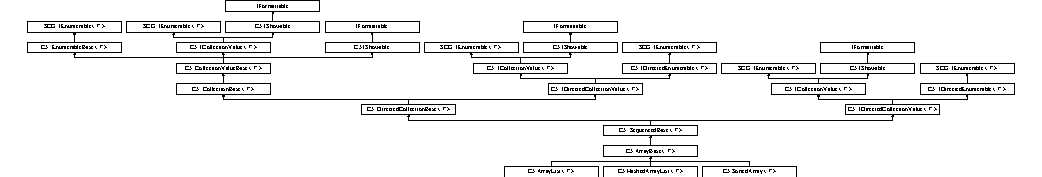
\includegraphics[height=2.366197cm]{class_c5_1_1_array_base}
\end{center}
\end{figure}
\subsection*{Classes}
\begin{DoxyCompactItemize}
\item 
class \hyperlink{class_c5_1_1_array_base_1_1_range}{Range}
\begin{DoxyCompactList}\small\item\em A helper class for defining results of interval queries on array based collections. \end{DoxyCompactList}\end{DoxyCompactItemize}
\subsection*{Public Member Functions}
\begin{DoxyCompactItemize}
\item 
virtual void \hyperlink{class_c5_1_1_array_base_abfee2ce913abdf40245562982f40a496}{Clear} ()
\begin{DoxyCompactList}\small\item\em Remove all items and reset size of internal array container. \end{DoxyCompactList}\item 
override T\mbox{[}$\,$\mbox{]} \hyperlink{class_c5_1_1_array_base_a16ffcc583a32065194b3ea27d4a43cd4}{To\+Array} ()
\begin{DoxyCompactList}\small\item\em Create an array containing (copies) of the items of this collection in enumeration order. \end{DoxyCompactList}\item 
virtual bool \hyperlink{class_c5_1_1_array_base_a45363fe7b6709bba1e37094d2cd5bfdf}{Check} ()
\begin{DoxyCompactList}\small\item\em Perform an internal consistency (invariant) test on the array base. \end{DoxyCompactList}\item 
override \hyperlink{interface_c5_1_1_i_directed_collection_value}{I\+Directed\+Collection\+Value}$<$ T $>$ \hyperlink{class_c5_1_1_array_base_a11fbdc5f71bb41de404f3bd91e3a92b3}{Backwards} ()
\begin{DoxyCompactList}\small\item\em Create a directed collection with the same contents as this one, but opposite enumeration sequence. \end{DoxyCompactList}\item 
override T \hyperlink{class_c5_1_1_array_base_a1d5f2551ce0fb795a5f2105fcb958de8}{Choose} ()
\begin{DoxyCompactList}\small\item\em Choose some item of this collection. The result is the last item in the internal array, making it efficient to remove. \end{DoxyCompactList}\item 
override S\+C\+G.\+I\+Enumerator$<$ T $>$ \hyperlink{class_c5_1_1_array_base_a84a54c5fa039db32e27ca45c6b0cea85}{Get\+Enumerator} ()
\begin{DoxyCompactList}\small\item\em Create an enumerator for this array based collection. \end{DoxyCompactList}\end{DoxyCompactItemize}
\subsection*{Protected Member Functions}
\begin{DoxyCompactItemize}
\item 
virtual void \hyperlink{class_c5_1_1_array_base_a6e32bc0bafd9263e2ccb18a5fedb032d}{expand} ()
\begin{DoxyCompactList}\small\item\em Double the size of the internal array. \end{DoxyCompactList}\item 
virtual void \hyperlink{class_c5_1_1_array_base_a5f2dcfe8c4c68077aa1b6c80a2d179c6}{expand} (int newcapacity, int newsize)
\begin{DoxyCompactList}\small\item\em Expand the internal array container. \end{DoxyCompactList}\item 
virtual void \hyperlink{class_c5_1_1_array_base_a5e47a614cf3a44d6657b5fa89e2ac26c}{insert} (int i, T item)
\begin{DoxyCompactList}\small\item\em Insert an item at a specific index, moving items to the right upwards and expanding the array if necessary. \end{DoxyCompactList}\item 
\hyperlink{class_c5_1_1_array_base_ae5aadcdb3a4f02dc7c00beff944970ba}{Array\+Base} (int capacity, S\+C\+G.\+I\+Equality\+Comparer$<$ T $>$ \hyperlink{class_c5_1_1_collection_base_a95e343400be0e8f3f8d6310f1aaf2cc6}{itemequality\+Comparer})
\begin{DoxyCompactList}\small\item\em Create an empty \hyperlink{class_c5_1_1_array_base}{Array\+Base} object. \end{DoxyCompactList}\end{DoxyCompactItemize}
\subsection*{Protected Attributes}
\begin{DoxyCompactItemize}
\item 
T\mbox{[}$\,$\mbox{]} \hyperlink{class_c5_1_1_array_base_a93d269a72f2299ba18b61ceb65590bdf}{array}
\begin{DoxyCompactList}\small\item\em The actual internal array container. Will be extended on demand. \end{DoxyCompactList}\item 
int \hyperlink{class_c5_1_1_array_base_a2fff33ea372907c015262a3041b2f2af}{offset}
\begin{DoxyCompactList}\small\item\em The offset into the internal array container of the first item. The offset is 0 for a base dynamic array and may be positive for an updatable view into a base dynamic array. \end{DoxyCompactList}\end{DoxyCompactItemize}
\subsection*{Properties}
\begin{DoxyCompactItemize}
\item 
virtual \hyperlink{interface_c5_1_1_i_directed_collection_value}{I\+Directed\+Collection\+Value}$<$ T $>$ \hyperlink{class_c5_1_1_array_base_a20e7840830115ed99dbd9054d714f7c7}{this\mbox{[}int start, int count\mbox{]}}\hspace{0.3cm}{\ttfamily  \mbox{[}get\mbox{]}}
\end{DoxyCompactItemize}
\subsection*{Additional Inherited Members}


\subsection{Detailed Description}
Base class for collection classes of dynamic array type implementations. 



\subsection{Constructor \& Destructor Documentation}
\hypertarget{class_c5_1_1_array_base_ae5aadcdb3a4f02dc7c00beff944970ba}{}\index{C5\+::\+Array\+Base@{C5\+::\+Array\+Base}!Array\+Base@{Array\+Base}}
\index{Array\+Base@{Array\+Base}!C5\+::\+Array\+Base@{C5\+::\+Array\+Base}}
\subsubsection[{Array\+Base(int capacity, S\+C\+G.\+I\+Equality\+Comparer$<$ T $>$ itemequality\+Comparer)}]{\setlength{\rightskip}{0pt plus 5cm}{\bf C5.\+Array\+Base}$<$ T $>$.{\bf Array\+Base} (
\begin{DoxyParamCaption}
\item[{int}]{capacity, }
\item[{S\+C\+G.\+I\+Equality\+Comparer$<$ T $>$}]{itemequality\+Comparer}
\end{DoxyParamCaption}
)\hspace{0.3cm}{\ttfamily [protected]}}\label{class_c5_1_1_array_base_ae5aadcdb3a4f02dc7c00beff944970ba}


Create an empty \hyperlink{class_c5_1_1_array_base}{Array\+Base} object. 


\begin{DoxyParams}{Parameters}
{\em capacity} & The initial capacity of the internal array container. Will be rounded upwards to the nearest power of 2 greater than or equal to 8.\\
\hline
{\em itemequality\+Comparer} & The item equality\+Comparer to use, primarily for item equality\\
\hline
\end{DoxyParams}


\subsection{Member Function Documentation}
\hypertarget{class_c5_1_1_array_base_a11fbdc5f71bb41de404f3bd91e3a92b3}{}\index{C5\+::\+Array\+Base@{C5\+::\+Array\+Base}!Backwards@{Backwards}}
\index{Backwards@{Backwards}!C5\+::\+Array\+Base@{C5\+::\+Array\+Base}}
\subsubsection[{Backwards()}]{\setlength{\rightskip}{0pt plus 5cm}override {\bf I\+Directed\+Collection\+Value}$<$T$>$ {\bf C5.\+Array\+Base}$<$ T $>$.Backwards (
\begin{DoxyParamCaption}
{}
\end{DoxyParamCaption}
)\hspace{0.3cm}{\ttfamily [virtual]}}\label{class_c5_1_1_array_base_a11fbdc5f71bb41de404f3bd91e3a92b3}


Create a directed collection with the same contents as this one, but opposite enumeration sequence. 

\begin{DoxyReturn}{Returns}
The mirrored collection.
\end{DoxyReturn}


Implements \hyperlink{class_c5_1_1_directed_collection_base_a9a4c7d6571ff7d78ea5adcb0d8264ff1}{C5.\+Directed\+Collection\+Base$<$ T $>$}.

\hypertarget{class_c5_1_1_array_base_a45363fe7b6709bba1e37094d2cd5bfdf}{}\index{C5\+::\+Array\+Base@{C5\+::\+Array\+Base}!Check@{Check}}
\index{Check@{Check}!C5\+::\+Array\+Base@{C5\+::\+Array\+Base}}
\subsubsection[{Check()}]{\setlength{\rightskip}{0pt plus 5cm}virtual bool {\bf C5.\+Array\+Base}$<$ T $>$.Check (
\begin{DoxyParamCaption}
{}
\end{DoxyParamCaption}
)\hspace{0.3cm}{\ttfamily [virtual]}}\label{class_c5_1_1_array_base_a45363fe7b6709bba1e37094d2cd5bfdf}


Perform an internal consistency (invariant) test on the array base. 

\begin{DoxyReturn}{Returns}
True if test succeeds.
\end{DoxyReturn}


Reimplemented in \hyperlink{class_c5_1_1_hashed_array_list_aed94ab3e8f52b3cd4b7825b12d6876b2}{C5.\+Hashed\+Array\+List$<$ T $>$}, \hyperlink{class_c5_1_1_array_list_adf389b80c82b6f6164c275e735148eed}{C5.\+Array\+List$<$ T $>$}, and \hyperlink{class_c5_1_1_sorted_array_a1b4c759074c4171089f65156607501d4}{C5.\+Sorted\+Array$<$ T $>$}.

\hypertarget{class_c5_1_1_array_base_a1d5f2551ce0fb795a5f2105fcb958de8}{}\index{C5\+::\+Array\+Base@{C5\+::\+Array\+Base}!Choose@{Choose}}
\index{Choose@{Choose}!C5\+::\+Array\+Base@{C5\+::\+Array\+Base}}
\subsubsection[{Choose()}]{\setlength{\rightskip}{0pt plus 5cm}override T {\bf C5.\+Array\+Base}$<$ T $>$.Choose (
\begin{DoxyParamCaption}
{}
\end{DoxyParamCaption}
)}\label{class_c5_1_1_array_base_a1d5f2551ce0fb795a5f2105fcb958de8}


Choose some item of this collection. The result is the last item in the internal array, making it efficient to remove. 


\begin{DoxyExceptions}{Exceptions}
{\em \hyperlink{class_c5_1_1_no_such_item_exception}{No\+Such\+Item\+Exception}} & if collection is empty.\\
\hline
\end{DoxyExceptions}
\begin{DoxyReturn}{Returns}

\end{DoxyReturn}


Implements \hyperlink{interface_c5_1_1_i_collection_value_af72d52ddd8ea4130d508e1cf020cf7eb}{C5.\+I\+Collection\+Value$<$ T $>$}.

\hypertarget{class_c5_1_1_array_base_abfee2ce913abdf40245562982f40a496}{}\index{C5\+::\+Array\+Base@{C5\+::\+Array\+Base}!Clear@{Clear}}
\index{Clear@{Clear}!C5\+::\+Array\+Base@{C5\+::\+Array\+Base}}
\subsubsection[{Clear()}]{\setlength{\rightskip}{0pt plus 5cm}virtual void {\bf C5.\+Array\+Base}$<$ T $>$.Clear (
\begin{DoxyParamCaption}
{}
\end{DoxyParamCaption}
)\hspace{0.3cm}{\ttfamily [virtual]}}\label{class_c5_1_1_array_base_abfee2ce913abdf40245562982f40a496}


Remove all items and reset size of internal array container. 



Reimplemented in \hyperlink{class_c5_1_1_hashed_array_list_aeca323e5f962607ee4384549aaba5d28}{C5.\+Hashed\+Array\+List$<$ T $>$}, \hyperlink{class_c5_1_1_array_list_a1ed4a8838cc6a215101b6af156e7da08}{C5.\+Array\+List$<$ T $>$}, and \hyperlink{class_c5_1_1_sorted_array_ae316e2061d7224288fefe5cc3a848935}{C5.\+Sorted\+Array$<$ T $>$}.

\hypertarget{class_c5_1_1_array_base_a6e32bc0bafd9263e2ccb18a5fedb032d}{}\index{C5\+::\+Array\+Base@{C5\+::\+Array\+Base}!expand@{expand}}
\index{expand@{expand}!C5\+::\+Array\+Base@{C5\+::\+Array\+Base}}
\subsubsection[{expand()}]{\setlength{\rightskip}{0pt plus 5cm}virtual void {\bf C5.\+Array\+Base}$<$ T $>$.expand (
\begin{DoxyParamCaption}
{}
\end{DoxyParamCaption}
)\hspace{0.3cm}{\ttfamily [protected]}, {\ttfamily [virtual]}}\label{class_c5_1_1_array_base_a6e32bc0bafd9263e2ccb18a5fedb032d}


Double the size of the internal array. 



Reimplemented in \hyperlink{class_c5_1_1_hashed_array_list_a4dce92728aada5e2d56902d0565247ff}{C5.\+Hashed\+Array\+List$<$ T $>$}, and \hyperlink{class_c5_1_1_array_list_a048d68f4ca0b66dbc9976c957b75d545}{C5.\+Array\+List$<$ T $>$}.

\hypertarget{class_c5_1_1_array_base_a5f2dcfe8c4c68077aa1b6c80a2d179c6}{}\index{C5\+::\+Array\+Base@{C5\+::\+Array\+Base}!expand@{expand}}
\index{expand@{expand}!C5\+::\+Array\+Base@{C5\+::\+Array\+Base}}
\subsubsection[{expand(int newcapacity, int newsize)}]{\setlength{\rightskip}{0pt plus 5cm}virtual void {\bf C5.\+Array\+Base}$<$ T $>$.expand (
\begin{DoxyParamCaption}
\item[{int}]{newcapacity, }
\item[{int}]{newsize}
\end{DoxyParamCaption}
)\hspace{0.3cm}{\ttfamily [protected]}, {\ttfamily [virtual]}}\label{class_c5_1_1_array_base_a5f2dcfe8c4c68077aa1b6c80a2d179c6}


Expand the internal array container. 


\begin{DoxyParams}{Parameters}
{\em newcapacity} & The new size of the internal array -\/ will be rounded upwards to a power of 2.\\
\hline
{\em newsize} & The (new) size of the (base) collection.\\
\hline
\end{DoxyParams}


Reimplemented in \hyperlink{class_c5_1_1_hashed_array_list_ae227e09958e8ce6eea7e0132ecd1a6aa}{C5.\+Hashed\+Array\+List$<$ T $>$}, and \hyperlink{class_c5_1_1_array_list_a08932223ebb743866c92756cbdee059b}{C5.\+Array\+List$<$ T $>$}.

\hypertarget{class_c5_1_1_array_base_a84a54c5fa039db32e27ca45c6b0cea85}{}\index{C5\+::\+Array\+Base@{C5\+::\+Array\+Base}!Get\+Enumerator@{Get\+Enumerator}}
\index{Get\+Enumerator@{Get\+Enumerator}!C5\+::\+Array\+Base@{C5\+::\+Array\+Base}}
\subsubsection[{Get\+Enumerator()}]{\setlength{\rightskip}{0pt plus 5cm}override S\+C\+G.\+I\+Enumerator$<$T$>$ {\bf C5.\+Array\+Base}$<$ T $>$.Get\+Enumerator (
\begin{DoxyParamCaption}
{}
\end{DoxyParamCaption}
)\hspace{0.3cm}{\ttfamily [virtual]}}\label{class_c5_1_1_array_base_a84a54c5fa039db32e27ca45c6b0cea85}


Create an enumerator for this array based collection. 

\begin{DoxyReturn}{Returns}
The enumerator
\end{DoxyReturn}


Implements \hyperlink{class_c5_1_1_sequenced_base_a07d117175b630fd7f87f6e61b05259dc}{C5.\+Sequenced\+Base$<$ T $>$}.

\hypertarget{class_c5_1_1_array_base_a5e47a614cf3a44d6657b5fa89e2ac26c}{}\index{C5\+::\+Array\+Base@{C5\+::\+Array\+Base}!insert@{insert}}
\index{insert@{insert}!C5\+::\+Array\+Base@{C5\+::\+Array\+Base}}
\subsubsection[{insert(int i, T item)}]{\setlength{\rightskip}{0pt plus 5cm}virtual void {\bf C5.\+Array\+Base}$<$ T $>$.insert (
\begin{DoxyParamCaption}
\item[{int}]{i, }
\item[{T}]{item}
\end{DoxyParamCaption}
)\hspace{0.3cm}{\ttfamily [protected]}, {\ttfamily [virtual]}}\label{class_c5_1_1_array_base_a5e47a614cf3a44d6657b5fa89e2ac26c}


Insert an item at a specific index, moving items to the right upwards and expanding the array if necessary. 


\begin{DoxyParams}{Parameters}
{\em i} & The index at which to insert.\\
\hline
{\em item} & The item to insert.\\
\hline
\end{DoxyParams}


Reimplemented in \hyperlink{class_c5_1_1_hashed_array_list_a70d3534f5dcf4e6b4c041ffc58dbc830}{C5.\+Hashed\+Array\+List$<$ T $>$}, and \hyperlink{class_c5_1_1_array_list_aadbaf3c60c27cd68711d9f0098e02ca0}{C5.\+Array\+List$<$ T $>$}.

\hypertarget{class_c5_1_1_array_base_a16ffcc583a32065194b3ea27d4a43cd4}{}\index{C5\+::\+Array\+Base@{C5\+::\+Array\+Base}!To\+Array@{To\+Array}}
\index{To\+Array@{To\+Array}!C5\+::\+Array\+Base@{C5\+::\+Array\+Base}}
\subsubsection[{To\+Array()}]{\setlength{\rightskip}{0pt plus 5cm}override T \mbox{[}$\,$\mbox{]} {\bf C5.\+Array\+Base}$<$ T $>$.To\+Array (
\begin{DoxyParamCaption}
{}
\end{DoxyParamCaption}
)}\label{class_c5_1_1_array_base_a16ffcc583a32065194b3ea27d4a43cd4}


Create an array containing (copies) of the items of this collection in enumeration order. 

\begin{DoxyReturn}{Returns}
The new array
\end{DoxyReturn}


Implements \hyperlink{interface_c5_1_1_i_collection_value_ad76547324e71a04e92076b2e55239bbb}{C5.\+I\+Collection\+Value$<$ T $>$}.



\subsection{Member Data Documentation}
\hypertarget{class_c5_1_1_array_base_a93d269a72f2299ba18b61ceb65590bdf}{}\index{C5\+::\+Array\+Base@{C5\+::\+Array\+Base}!array@{array}}
\index{array@{array}!C5\+::\+Array\+Base@{C5\+::\+Array\+Base}}
\subsubsection[{array}]{\setlength{\rightskip}{0pt plus 5cm}T \mbox{[}$\,$\mbox{]} {\bf C5.\+Array\+Base}$<$ T $>$.array\hspace{0.3cm}{\ttfamily [protected]}}\label{class_c5_1_1_array_base_a93d269a72f2299ba18b61ceb65590bdf}


The actual internal array container. Will be extended on demand. 

\hypertarget{class_c5_1_1_array_base_a2fff33ea372907c015262a3041b2f2af}{}\index{C5\+::\+Array\+Base@{C5\+::\+Array\+Base}!offset@{offset}}
\index{offset@{offset}!C5\+::\+Array\+Base@{C5\+::\+Array\+Base}}
\subsubsection[{offset}]{\setlength{\rightskip}{0pt plus 5cm}int {\bf C5.\+Array\+Base}$<$ T $>$.offset\hspace{0.3cm}{\ttfamily [protected]}}\label{class_c5_1_1_array_base_a2fff33ea372907c015262a3041b2f2af}


The offset into the internal array container of the first item. The offset is 0 for a base dynamic array and may be positive for an updatable view into a base dynamic array. 



\subsection{Property Documentation}
\hypertarget{class_c5_1_1_array_base_a20e7840830115ed99dbd9054d714f7c7}{}\index{C5\+::\+Array\+Base@{C5\+::\+Array\+Base}!this\mbox{[}int start, int count\mbox{]}@{this[int start, int count]}}
\index{this\mbox{[}int start, int count\mbox{]}@{this[int start, int count]}!C5\+::\+Array\+Base@{C5\+::\+Array\+Base}}
\subsubsection[{this[int start, int count]}]{\setlength{\rightskip}{0pt plus 5cm}virtual {\bf I\+Directed\+Collection\+Value}$<$T$>$ {\bf C5.\+Array\+Base}$<$ T $>$.this\mbox{[}int start, int count\mbox{]}\hspace{0.3cm}{\ttfamily [get]}}\label{class_c5_1_1_array_base_a20e7840830115ed99dbd9054d714f7c7}





\begin{DoxyExceptions}{Exceptions}
{\em Argument\+Out\+Of\+Range\+Exception} & If the arguments does not describe a valid range in the indexed collection, cf. M\+:\+C5.\+Collection\+Base`1.\+check\+Range(\+System.\+Int32,\+System.\+Int32).\\
\hline
\end{DoxyExceptions}


The directed collection of items in a specific index interval.


\begin{DoxyParams}{Parameters}
{\em start} & The low index of the interval (inclusive).\\
\hline
{\em count} & The size of the range.\\
\hline
\end{DoxyParams}


The documentation for this class was generated from the following file\+:\begin{DoxyCompactItemize}
\item 
C\+:/\+Users/rasmusl/\+Source/\+Repos/\+C5/\+C5/\hyperlink{_collections_8cs}{Collections.\+cs}\end{DoxyCompactItemize}

\hypertarget{class_c5_1_1_array_list}{}\section{C5.\+Array\+List$<$ T $>$ Class Template Reference}
\label{class_c5_1_1_array_list}\index{C5.\+Array\+List$<$ T $>$@{C5.\+Array\+List$<$ T $>$}}


A list collection based on a plain dynamic array data structure. Expansion of the internal array is performed by doubling on demand. The internal array is only shrinked by the Clear method.  


Inheritance diagram for C5.\+Array\+List$<$ T $>$\+:\begin{figure}[H]
\begin{center}
\leavevmode
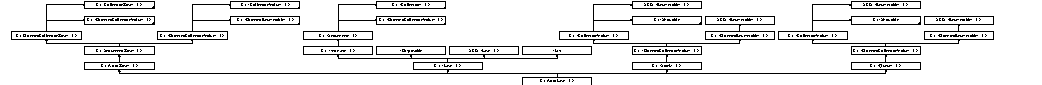
\includegraphics[height=1.126760cm]{class_c5_1_1_array_list}
\end{center}
\end{figure}
\subsection*{Public Member Functions}
\begin{DoxyCompactItemize}
\item 
\hyperlink{class_c5_1_1_array_list_afc3bc6f60671256fe1c9c6ade8b1ef45}{Array\+List} ()
\begin{DoxyCompactList}\small\item\em Create an array list with default item equality\+Comparer and initial capacity 8 items. \end{DoxyCompactList}\item 
\hyperlink{class_c5_1_1_array_list_aaed80fc15085f472c99a317acceb1010}{Array\+List} (S\+C\+G.\+I\+Equality\+Comparer$<$ T $>$ \hyperlink{class_c5_1_1_collection_base_a95e343400be0e8f3f8d6310f1aaf2cc6}{itemequality\+Comparer})
\begin{DoxyCompactList}\small\item\em Create an array list with external item equality\+Comparer and initial capacity 8 items. \end{DoxyCompactList}\item 
\hyperlink{class_c5_1_1_array_list_a4bf6bc33f17a8ba8978e24a0058d8dd7}{Array\+List} (int capacity)
\begin{DoxyCompactList}\small\item\em Create an array list with default item equality\+Comparer and prescribed initial capacity. \end{DoxyCompactList}\item 
\hyperlink{class_c5_1_1_array_list_a0ed9d4461ca964278f8221ed2b1b829a}{Array\+List} (int capacity, S\+C\+G.\+I\+Equality\+Comparer$<$ T $>$ \hyperlink{class_c5_1_1_collection_base_a95e343400be0e8f3f8d6310f1aaf2cc6}{itemequality\+Comparer})
\begin{DoxyCompactList}\small\item\em Create an array list with external item equality\+Comparer and prescribed initial capacity. \end{DoxyCompactList}\item 
virtual void \hyperlink{class_c5_1_1_array_list_a4716054131d8c9c4a60eefe0e3d9e97f}{Insert} (int index, T item)
\begin{DoxyCompactList}\small\item\em Insert an item at a specific index location in this list. /summary$>$ 
\begin{DoxyExceptions}{Exceptions}
{\em Index\+Out\+Of\+Range\+Exception} & if i is negative or $>$ the size of the collection. \\
\hline
\end{DoxyExceptions}

\begin{DoxyParams}{Parameters}
{\em index} & The index at which to insert.\\
\hline
{\em item} & The item to insert.\\
\hline
\end{DoxyParams}
\end{DoxyCompactList}\item 
void \hyperlink{class_c5_1_1_array_list_a9622480e8a1e187bb4174cd1d149b1f9}{Insert} (\hyperlink{interface_c5_1_1_i_list}{I\+List}$<$ T $>$ pointer, T item)
\begin{DoxyCompactList}\small\item\em Insert an item at the end of a compatible view, used as a pointer. \end{DoxyCompactList}\item 
virtual void \hyperlink{class_c5_1_1_array_list_a587910564b15fa1c71b6ba72ff7a4395}{Insert\+All} (int index, S\+C\+G.\+I\+Enumerable$<$ T $>$ items)
\begin{DoxyCompactList}\small\item\em Insert into this list all items from an enumerable collection starting at a particular index. \end{DoxyCompactList}\item 
virtual void \hyperlink{class_c5_1_1_array_list_a272dc95d5ca8c2ce1b3ab43e3c56a4ce}{Insert\+First} (T item)
\begin{DoxyCompactList}\small\item\em Insert an item at the front of this list; \end{DoxyCompactList}\item 
virtual void \hyperlink{class_c5_1_1_array_list_a31ce1aee48da6e5e90791c61af922a3b}{Insert\+Last} (T item)
\begin{DoxyCompactList}\small\item\em Insert an item at the back of this list. \end{DoxyCompactList}\item 
virtual \hyperlink{interface_c5_1_1_i_list}{I\+List}$<$ T $>$ \hyperlink{class_c5_1_1_array_list_a8d970094faac5c6940db43796264b751}{Find\+All} (Func$<$ T, bool $>$ filter)
\begin{DoxyCompactList}\small\item\em Create a new list consisting of the items of this list satisfying a certain predicate. \end{DoxyCompactList}\item 
virtual \hyperlink{interface_c5_1_1_i_list}{I\+List}$<$ V $>$ \hyperlink{class_c5_1_1_array_list_a7a973a5950c1f27d95cce3d8d3a5979f}{Map$<$ V $>$} (Func$<$ T, V $>$ mapper)
\begin{DoxyCompactList}\small\item\em Create a new list consisting of the results of mapping all items of this list. The new list will use the default item equality\+Comparer for the item type V. \end{DoxyCompactList}\item 
virtual \hyperlink{interface_c5_1_1_i_list}{I\+List}$<$ V $>$ \hyperlink{class_c5_1_1_array_list_a3cc88a23901441ffca7b03f8445c6c6a}{Map$<$ V $>$} (Func$<$ T, V $>$ mapper, S\+C\+G.\+I\+Equality\+Comparer$<$ V $>$ \hyperlink{class_c5_1_1_collection_base_a95e343400be0e8f3f8d6310f1aaf2cc6}{itemequality\+Comparer})
\begin{DoxyCompactList}\small\item\em Create a new list consisting of the results of mapping all items of this list. The new list will use a specified item equality\+Comparer for the item type. \end{DoxyCompactList}\item 
virtual T \hyperlink{class_c5_1_1_array_list_a0bdb83e1cd5d4e6a75440f75c0fa7c9b}{Remove} ()
\begin{DoxyCompactList}\small\item\em Remove one item from the list\+: from the front if \end{DoxyCompactList}\item 
virtual T \hyperlink{class_c5_1_1_array_list_aaf9d886025d96e91a9275055a37b984f}{Remove\+First} ()
\begin{DoxyCompactList}\small\item\em Remove one item from the fromnt of the list. \end{DoxyCompactList}\item 
virtual T \hyperlink{class_c5_1_1_array_list_af26267e25450db0612a4eeb8210560c5}{Remove\+Last} ()
\begin{DoxyCompactList}\small\item\em Remove one item from the back of the list. \end{DoxyCompactList}\item 
virtual \hyperlink{interface_c5_1_1_i_list}{I\+List}$<$ T $>$ \hyperlink{class_c5_1_1_array_list_a07ada18bdafce7fc420fcd54f4da17c9}{View} (int start, int count)
\begin{DoxyCompactList}\small\item\em Create a list view on this list. \end{DoxyCompactList}\item 
virtual \hyperlink{interface_c5_1_1_i_list}{I\+List}$<$ T $>$ \hyperlink{class_c5_1_1_array_list_ae51aa95d71cfbf4ac68610d6285a308e}{View\+Of} (T item)
\begin{DoxyCompactList}\small\item\em Create a list view on this list containing the (first) occurrence of a particular item. \end{DoxyCompactList}\item 
virtual \hyperlink{interface_c5_1_1_i_list}{I\+List}$<$ T $>$ \hyperlink{class_c5_1_1_array_list_a501ef3474fc833061931a134daa2cab2}{Last\+View\+Of} (T item)
\begin{DoxyCompactList}\small\item\em Create a list view on this list containing the last occurrence of a particular item. \end{DoxyCompactList}\item 
virtual \hyperlink{interface_c5_1_1_i_list}{I\+List}$<$ T $>$ \hyperlink{class_c5_1_1_array_list_ae3a767b85e9ce23fadec95048a265bf4}{Slide} (int \hyperlink{class_c5_1_1_array_base_a2fff33ea372907c015262a3041b2f2af}{offset})
\begin{DoxyCompactList}\small\item\em Slide this list view along the underlying list. \end{DoxyCompactList}\item 
virtual \hyperlink{interface_c5_1_1_i_list}{I\+List}$<$ T $>$ \hyperlink{class_c5_1_1_array_list_ab20264e4ddd5209180c5d352ab85a17f}{Slide} (int \hyperlink{class_c5_1_1_array_base_a2fff33ea372907c015262a3041b2f2af}{offset}, int \hyperlink{class_c5_1_1_collection_base_ab524b118754a5a8290b6528511272833}{size})
\begin{DoxyCompactList}\small\item\em Slide this list view along the underlying list, changing its size. \end{DoxyCompactList}\item 
virtual bool \hyperlink{class_c5_1_1_array_list_adac943600e590e256dc302cb985e9e28}{Try\+Slide} (int \hyperlink{class_c5_1_1_array_base_a2fff33ea372907c015262a3041b2f2af}{offset})
\item 
virtual bool \hyperlink{class_c5_1_1_array_list_ae36f7c07dba092711b1a2a0068d54619}{Try\+Slide} (int \hyperlink{class_c5_1_1_array_base_a2fff33ea372907c015262a3041b2f2af}{offset}, int \hyperlink{class_c5_1_1_collection_base_ab524b118754a5a8290b6528511272833}{size})
\item 
virtual \hyperlink{interface_c5_1_1_i_list}{I\+List}$<$ T $>$ \hyperlink{class_c5_1_1_array_list_ac28db3fe49e52107a54e7a33dabb67c2}{Span} (\hyperlink{interface_c5_1_1_i_list}{I\+List}$<$ T $>$ other\+View)
\item 
virtual void \hyperlink{class_c5_1_1_array_list_ad5c4e9fcce3bdafcb4140b24e449b210}{Reverse} ()
\begin{DoxyCompactList}\small\item\em Reverst the list so the items are in the opposite sequence order. \end{DoxyCompactList}\item 
bool \hyperlink{class_c5_1_1_array_list_a9c15cf2f69d3459b4a22ecd854689768}{Is\+Sorted} ()
\begin{DoxyCompactList}\small\item\em Check if this list is sorted according to the default sorting order for the item type T, as defined by the T\+:\+C5.\+Comparer`1 class \end{DoxyCompactList}\item 
virtual bool \hyperlink{class_c5_1_1_array_list_a267b37f723053dcc17d03c789956332a}{Is\+Sorted} (S\+C\+G.\+I\+Comparer$<$ T $>$ c)
\begin{DoxyCompactList}\small\item\em Check if this list is sorted according to a specific sorting order. \end{DoxyCompactList}\item 
virtual void \hyperlink{class_c5_1_1_array_list_a2fa70a028357e88da185799b15a508cb}{Sort} ()
\begin{DoxyCompactList}\small\item\em Sort the items of the list according to the default sorting order for the item type T, as defined by the Comparer\mbox{[}T\mbox{]} class (T\+:\+C5.\+Comparer`1). \end{DoxyCompactList}\item 
virtual void \hyperlink{class_c5_1_1_array_list_af5c128e592dfdb043e8687bf3e3cad68}{Sort} (S\+C\+G.\+I\+Comparer$<$ T $>$ comparer)
\begin{DoxyCompactList}\small\item\em Sort the items of the list according to a specific sorting order. \end{DoxyCompactList}\item 
virtual void \hyperlink{class_c5_1_1_array_list_a8c7d42a5d4941fba55338f7e6a759049}{Shuffle} ()
\begin{DoxyCompactList}\small\item\em Randomly shuffle the items of this list. \end{DoxyCompactList}\item 
virtual void \hyperlink{class_c5_1_1_array_list_ae209e9cc5f70627d16a892705a11ff6f}{Shuffle} (Random rnd)
\begin{DoxyCompactList}\small\item\em Shuffle the items of this list according to a specific random source. \end{DoxyCompactList}\item 
virtual int \hyperlink{class_c5_1_1_array_list_ae94dff251b125331c450b396418bb1be}{Index\+Of} (T item)
\begin{DoxyCompactList}\small\item\em Search for an item in the list going forwrds from the start. \end{DoxyCompactList}\item 
virtual int \hyperlink{class_c5_1_1_array_list_af04d77e11483bfcfa1cac7fd88b57bc5}{Last\+Index\+Of} (T item)
\begin{DoxyCompactList}\small\item\em Search for an item in the list going backwords from the end. \end{DoxyCompactList}\item 
virtual T \hyperlink{class_c5_1_1_array_list_a0f3b4828a1c3ba06d035ad6f2aa491fc}{Remove\+At} (int index)
\begin{DoxyCompactList}\small\item\em Remove the item at a specific position of the list. \end{DoxyCompactList}\item 
virtual void \hyperlink{class_c5_1_1_array_list_aa4c6f08712ec985076e402d713e5a616}{Remove\+Interval} (int start, int count)
\begin{DoxyCompactList}\small\item\em Remove all items in an index interval. \end{DoxyCompactList}\item 
override int \hyperlink{class_c5_1_1_array_list_a4f75d053012574e34e670597aa392e6f}{Get\+Unsequenced\+Hash\+Code} ()
\item 
override bool \hyperlink{class_c5_1_1_array_list_a46753a14629243761d6056839747f23f}{Unsequenced\+Equals} (\hyperlink{interface_c5_1_1_i_collection}{I\+Collection}$<$ T $>$ that)
\item 
virtual bool \hyperlink{class_c5_1_1_array_list_a481c1d9104e4c5fbd4dd79be7a1e5c38}{Contains} (T item)
\begin{DoxyCompactList}\small\item\em Check if this collection contains (an item equivalent to according to the itemequality\+Comparer) a particular value. \end{DoxyCompactList}\item 
virtual bool \hyperlink{class_c5_1_1_array_list_a835191c794936ab62f751aaef835254d}{Find} (ref T item)
\begin{DoxyCompactList}\small\item\em Check if this collection contains an item equivalent according to the itemequality\+Comparer to a particular value. If so, return in the ref argument (a binary copy of) the actual value found. \end{DoxyCompactList}\item 
virtual bool \hyperlink{class_c5_1_1_array_list_af3b4372db9e6040a7b26ec773a17dd76}{Update} (T item)
\begin{DoxyCompactList}\small\item\em Check if this collection contains an item equivalent according to the itemequality\+Comparer to a particular value. If so, update the item in the collection to with a binary copy of the supplied value. This will only update the first mathching item. \end{DoxyCompactList}\item 
virtual bool \hyperlink{class_c5_1_1_array_list_a9ab8634f890942de1711e5a8de88f6cc}{Update} (T item, out T olditem)
\item 
virtual bool \hyperlink{class_c5_1_1_array_list_a35b8836d9228034409fc10e4dc5d7779}{Find\+Or\+Add} (ref T item)
\begin{DoxyCompactList}\small\item\em Check if this collection contains an item equivalent according to the itemequality\+Comparer to a particular value. If so, return in the ref argument (a binary copy of) the actual value found. Else, add the item to the collection. \end{DoxyCompactList}\item 
virtual bool \hyperlink{class_c5_1_1_array_list_a2f38168aaa805fc305be7800e2298b9f}{Update\+Or\+Add} (T item)
\begin{DoxyCompactList}\small\item\em Check if this collection contains an item equivalent according to the itemequality\+Comparer to a particular value. If so, update the item in the collection to with a binary copy of the supplied value. This will only update the first mathching item. \end{DoxyCompactList}\item 
virtual bool \hyperlink{class_c5_1_1_array_list_a5bb957a4a9d9d8fa6040c0fe1c9d1237}{Update\+Or\+Add} (T item, out T olditem)
\item 
virtual bool \hyperlink{class_c5_1_1_array_list_a8e3d348ba6d557785028bee0b9a25bf8}{Remove} (T item)
\begin{DoxyCompactList}\small\item\em Remove a particular item from this list. The item will be searched for from the end of the list if \end{DoxyCompactList}\item 
virtual bool \hyperlink{class_c5_1_1_array_list_adc146d07d67bf7e96f07fb604c83b2c9}{Remove} (T item, out T removeditem)
\begin{DoxyCompactList}\small\item\em Remove the first copy of a particular item from this collection if found. If an item was removed, report a binary copy of the actual item removed in the argument. The item will be searched for from the end of the list if \end{DoxyCompactList}\item 
virtual void \hyperlink{class_c5_1_1_array_list_aaa0409bfe3256b9e5749ff8710f89b45}{Remove\+All} (S\+C\+G.\+I\+Enumerable$<$ T $>$ items)
\begin{DoxyCompactList}\small\item\em Remove all items in another collection from this one, taking multiplicities into account. Matching items will be removed from the front. Current implementation is not optimal. \end{DoxyCompactList}\item 
override void \hyperlink{class_c5_1_1_array_list_a1ed4a8838cc6a215101b6af156e7da08}{Clear} ()
\begin{DoxyCompactList}\small\item\em Remove all items from this collection, resetting internal array size. \end{DoxyCompactList}\item 
virtual void \hyperlink{class_c5_1_1_array_list_a7f3f5674779507d03f9139dea24977a2}{Retain\+All} (S\+C\+G.\+I\+Enumerable$<$ T $>$ items)
\begin{DoxyCompactList}\small\item\em Remove all items not in some other collection from this one, taking multiplicities into account. Items are retained front first. \end{DoxyCompactList}\item 
virtual bool \hyperlink{class_c5_1_1_array_list_a59f882585e714af67e2ba7211e3d3595}{Contains\+All} (S\+C\+G.\+I\+Enumerable$<$ T $>$ items)
\begin{DoxyCompactList}\small\item\em Check if this collection contains all the values in another collection, taking multiplicities into account. Current implementation is not optimal. \end{DoxyCompactList}\item 
virtual int \hyperlink{class_c5_1_1_array_list_a64988ea7ea5325a0ee85d96ed32401dd}{Contains\+Count} (T item)
\begin{DoxyCompactList}\small\item\em Count the number of items of the collection equal to a particular value. Returns 0 if and only if the value is not in the collection. \end{DoxyCompactList}\item 
virtual \hyperlink{interface_c5_1_1_i_collection_value}{I\+Collection\+Value}$<$ T $>$ \hyperlink{class_c5_1_1_array_list_a3d9b907977cfdf33ae2dbb7176c22ec8}{Unique\+Items} ()
\item 
virtual \hyperlink{interface_c5_1_1_i_collection_value}{I\+Collection\+Value}$<$ \hyperlink{struct_c5_1_1_key_value_pair}{Key\+Value\+Pair}$<$ T, int $>$ $>$ \hyperlink{class_c5_1_1_array_list_a335c5003a3607d44e571f7fa444e75cb}{Item\+Multiplicities} ()
\item 
virtual void \hyperlink{class_c5_1_1_array_list_a375c1c5bb0d8b80208b32f90128f7347}{Remove\+All\+Copies} (T item)
\begin{DoxyCompactList}\small\item\em Remove all items equal to a given one. \end{DoxyCompactList}\item 
override bool \hyperlink{class_c5_1_1_array_list_adf389b80c82b6f6164c275e735148eed}{Check} ()
\begin{DoxyCompactList}\small\item\em Check the integrity of the internal data structures of this array list. \end{DoxyCompactList}\item 
virtual bool \hyperlink{class_c5_1_1_array_list_a31f07a779aa64ee15f6875ab74682cb5}{Add} (T item)
\begin{DoxyCompactList}\small\item\em Add an item to end of this list. \end{DoxyCompactList}\item 
virtual void \hyperlink{class_c5_1_1_array_list_ae84250369cc406ec412bc2962acdf9e4}{Add\+All} (S\+C\+G.\+I\+Enumerable$<$ T $>$ items)
\begin{DoxyCompactList}\small\item\em Add the elements from another collection to this collection. \end{DoxyCompactList}\item 
override S\+C\+G.\+I\+Enumerator$<$ T $>$ \hyperlink{class_c5_1_1_array_list_ae6c2dc2f2aa8c9952d3267a37e9de01a}{Get\+Enumerator} ()
\begin{DoxyCompactList}\small\item\em Create an enumerator for the collection \end{DoxyCompactList}\item 
virtual void \hyperlink{class_c5_1_1_array_list_a1eb4d5aadf670338e6402bf27fdc1b3a}{Push} (T item)
\begin{DoxyCompactList}\small\item\em Push an item to the top of the stack. \end{DoxyCompactList}\item 
virtual T \hyperlink{class_c5_1_1_array_list_aa9491c75f081e2680f2e9ad9a7875f7a}{Pop} ()
\begin{DoxyCompactList}\small\item\em Pop the item at the top of the stack from the stack. \end{DoxyCompactList}\item 
virtual void \hyperlink{class_c5_1_1_array_list_ac19b1fa4c34de8cf94afa85b325c5646}{Enqueue} (T item)
\begin{DoxyCompactList}\small\item\em Enqueue an item at the back of the queue. \end{DoxyCompactList}\item 
virtual T \hyperlink{class_c5_1_1_array_list_a82a4b5a21129d4cffe69fa53b9bfe827}{Dequeue} ()
\begin{DoxyCompactList}\small\item\em Dequeue an item from the front of the queue. \end{DoxyCompactList}\item 
virtual void \hyperlink{class_c5_1_1_array_list_a55ec641afe9eee899265a72119163e03}{Dispose} ()
\begin{DoxyCompactList}\small\item\em Invalidate this list. If a view, just invalidate the view. If not a view, invalidate the list and all views on it. \end{DoxyCompactList}\end{DoxyCompactItemize}
\subsection*{Protected Member Functions}
\begin{DoxyCompactItemize}
\item 
override void \hyperlink{class_c5_1_1_array_list_a048d68f4ca0b66dbc9976c957b75d545}{expand} ()
\begin{DoxyCompactList}\small\item\em Double the size of the internal array. \end{DoxyCompactList}\item 
override void \hyperlink{class_c5_1_1_array_list_a08932223ebb743866c92756cbdee059b}{expand} (int newcapacity, int newsize)
\begin{DoxyCompactList}\small\item\em Expand the internal array, resetting the index of the first unused element. \end{DoxyCompactList}\item 
override void \hyperlink{class_c5_1_1_array_list_a3d2755c3b8fdd5fc8d4b7b435a2002ff}{updatecheck} ()
\begin{DoxyCompactList}\small\item\em Check if it is valid to perform updates and increment stamp if so. \end{DoxyCompactList}\item 
override void \hyperlink{class_c5_1_1_array_list_a1ab3f3702bc6ac270a421479e90437dd}{modifycheck} (int \hyperlink{class_c5_1_1_collection_base_ae13bd5b482306a49a4d10654a9b8b064}{stamp})
\begin{DoxyCompactList}\small\item\em Check that the list has not been updated since a particular time. \end{DoxyCompactList}\item 
override void \hyperlink{class_c5_1_1_array_list_aadbaf3c60c27cd68711d9f0098e02ca0}{insert} (int i, T item)
\begin{DoxyCompactList}\small\item\em Internal version of Insert with no modification checks. \end{DoxyCompactList}\end{DoxyCompactItemize}
\subsection*{Properties}
\begin{DoxyCompactItemize}
\item 
override \hyperlink{namespace_c5_a9143bfd561fffa025d21561674758008}{Event\+Type\+Enum} \hyperlink{class_c5_1_1_array_list_a8560c6e1b75c9d706d2d2d2618269d4f}{Listenable\+Events}\hspace{0.3cm}{\ttfamily  \mbox{[}get\mbox{]}}
\item 
virtual T \hyperlink{class_c5_1_1_array_list_afbe0bbad61f1e2ac5105fe3a73d4d9c8}{First}\hspace{0.3cm}{\ttfamily  \mbox{[}get\mbox{]}}
\item 
virtual T \hyperlink{class_c5_1_1_array_list_a520a0e6f4b6b9038bc9ad63770c78a95}{Last}\hspace{0.3cm}{\ttfamily  \mbox{[}get\mbox{]}}
\item 
virtual bool \hyperlink{class_c5_1_1_array_list_afe367da5aabd34c3c4af20648deaf6a6}{F\+I\+F\+O}\hspace{0.3cm}{\ttfamily  \mbox{[}get, set\mbox{]}}
\begin{DoxyCompactList}\small\item\em Since \end{DoxyCompactList}\item 
virtual bool \hyperlink{class_c5_1_1_array_list_a8fca7fcada0dce088679de34c1cb9c37}{Is\+Fixed\+Size}\hspace{0.3cm}{\ttfamily  \mbox{[}get\mbox{]}}
\item 
virtual T \hyperlink{class_c5_1_1_array_list_a2a4990b7502658c6f8bbebe2a3eea351}{this\mbox{[}int index\mbox{]}}\hspace{0.3cm}{\ttfamily  \mbox{[}get, set\mbox{]}}
\begin{DoxyCompactList}\small\item\em On this list, this indexer is read/write. \end{DoxyCompactList}\item 
virtual \hyperlink{namespace_c5_a615ba88dcdaa8d5a3c5f833a73d7fad6}{Speed} \hyperlink{class_c5_1_1_array_list_ae98cfa9bac197c389bbb16159a116c04}{Indexing\+Speed}\hspace{0.3cm}{\ttfamily  \mbox{[}get\mbox{]}}
\item 
virtual \hyperlink{interface_c5_1_1_i_list}{I\+List}$<$ T $>$ \hyperlink{class_c5_1_1_array_list_a41d739fd8a2d169b3121cc05871323f0}{Underlying}\hspace{0.3cm}{\ttfamily  \mbox{[}get\mbox{]}}
\begin{DoxyCompactList}\small\item\em Null if this list is not a view. \end{DoxyCompactList}\item 
virtual int \hyperlink{class_c5_1_1_array_list_ae811cb2c92d313a6d4d54f31dd0caed5}{Offset}\hspace{0.3cm}{\ttfamily  \mbox{[}get\mbox{]}}
\item 
virtual bool \hyperlink{class_c5_1_1_array_list_a81012dc5309f8f7e24bf61b8eda60b45}{Is\+Valid}\hspace{0.3cm}{\ttfamily  \mbox{[}get\mbox{]}}
\item 
virtual \hyperlink{namespace_c5_a615ba88dcdaa8d5a3c5f833a73d7fad6}{Speed} \hyperlink{class_c5_1_1_array_list_a4ecabee5bf4516170750cf2bdf1384f0}{Contains\+Speed}\hspace{0.3cm}{\ttfamily  \mbox{[}get\mbox{]}}
\begin{DoxyCompactList}\small\item\em The value is symbolic indicating the type of asymptotic complexity in terms of the size of this collection (worst-\/case or amortized as relevant). \end{DoxyCompactList}\item 
virtual bool \hyperlink{class_c5_1_1_array_list_a543195d51a2e01b58772297e079f3a17}{Allows\+Duplicates}\hspace{0.3cm}{\ttfamily  \mbox{[}get\mbox{]}}
\item 
virtual bool \hyperlink{class_c5_1_1_array_list_a7aabcc197b80abbccc4b39497816ec4f}{Duplicates\+By\+Counting}\hspace{0.3cm}{\ttfamily  \mbox{[}get\mbox{]}}
\begin{DoxyCompactList}\small\item\em By convention this is true for any collection with set semantics. \end{DoxyCompactList}\item 
override int \hyperlink{class_c5_1_1_array_list_aee0f5d70dbc5ce43dfe5ca71f17e5913}{Count}\hspace{0.3cm}{\ttfamily  \mbox{[}get\mbox{]}}
\end{DoxyCompactItemize}
\subsection*{Additional Inherited Members}


\subsection{Detailed Description}
A list collection based on a plain dynamic array data structure. Expansion of the internal array is performed by doubling on demand. The internal array is only shrinked by the Clear method. 

{\itshape When the F\+I\+F\+O property is set to false this class works fine as a stack of T. When the F\+I\+F\+O property is set to true the class will function as a (F\+I\+F\+O) queue but very inefficiently, use a \hyperlink{class_c5_1_1_linked_list}{Linked\+List} (T\+:\+C5.\+Linked\+List`1) instead.} 

\subsection{Constructor \& Destructor Documentation}
\hypertarget{class_c5_1_1_array_list_afc3bc6f60671256fe1c9c6ade8b1ef45}{}\index{C5\+::\+Array\+List@{C5\+::\+Array\+List}!Array\+List@{Array\+List}}
\index{Array\+List@{Array\+List}!C5\+::\+Array\+List@{C5\+::\+Array\+List}}
\subsubsection[{Array\+List()}]{\setlength{\rightskip}{0pt plus 5cm}{\bf C5.\+Array\+List}$<$ T $>$.{\bf Array\+List} (
\begin{DoxyParamCaption}
{}
\end{DoxyParamCaption}
)}\label{class_c5_1_1_array_list_afc3bc6f60671256fe1c9c6ade8b1ef45}


Create an array list with default item equality\+Comparer and initial capacity 8 items. 

\hypertarget{class_c5_1_1_array_list_aaed80fc15085f472c99a317acceb1010}{}\index{C5\+::\+Array\+List@{C5\+::\+Array\+List}!Array\+List@{Array\+List}}
\index{Array\+List@{Array\+List}!C5\+::\+Array\+List@{C5\+::\+Array\+List}}
\subsubsection[{Array\+List(\+S\+C\+G.\+I\+Equality\+Comparer$<$ T $>$ itemequality\+Comparer)}]{\setlength{\rightskip}{0pt plus 5cm}{\bf C5.\+Array\+List}$<$ T $>$.{\bf Array\+List} (
\begin{DoxyParamCaption}
\item[{S\+C\+G.\+I\+Equality\+Comparer$<$ T $>$}]{itemequality\+Comparer}
\end{DoxyParamCaption}
)}\label{class_c5_1_1_array_list_aaed80fc15085f472c99a317acceb1010}


Create an array list with external item equality\+Comparer and initial capacity 8 items. 


\begin{DoxyParams}{Parameters}
{\em itemequality\+Comparer} & The external item equality\+S\+C\+G.\+Comparer\\
\hline
\end{DoxyParams}
\hypertarget{class_c5_1_1_array_list_a4bf6bc33f17a8ba8978e24a0058d8dd7}{}\index{C5\+::\+Array\+List@{C5\+::\+Array\+List}!Array\+List@{Array\+List}}
\index{Array\+List@{Array\+List}!C5\+::\+Array\+List@{C5\+::\+Array\+List}}
\subsubsection[{Array\+List(int capacity)}]{\setlength{\rightskip}{0pt plus 5cm}{\bf C5.\+Array\+List}$<$ T $>$.{\bf Array\+List} (
\begin{DoxyParamCaption}
\item[{int}]{capacity}
\end{DoxyParamCaption}
)}\label{class_c5_1_1_array_list_a4bf6bc33f17a8ba8978e24a0058d8dd7}


Create an array list with default item equality\+Comparer and prescribed initial capacity. 


\begin{DoxyParams}{Parameters}
{\em capacity} & The prescribed capacity\\
\hline
\end{DoxyParams}
\hypertarget{class_c5_1_1_array_list_a0ed9d4461ca964278f8221ed2b1b829a}{}\index{C5\+::\+Array\+List@{C5\+::\+Array\+List}!Array\+List@{Array\+List}}
\index{Array\+List@{Array\+List}!C5\+::\+Array\+List@{C5\+::\+Array\+List}}
\subsubsection[{Array\+List(int capacity, S\+C\+G.\+I\+Equality\+Comparer$<$ T $>$ itemequality\+Comparer)}]{\setlength{\rightskip}{0pt plus 5cm}{\bf C5.\+Array\+List}$<$ T $>$.{\bf Array\+List} (
\begin{DoxyParamCaption}
\item[{int}]{capacity, }
\item[{S\+C\+G.\+I\+Equality\+Comparer$<$ T $>$}]{itemequality\+Comparer}
\end{DoxyParamCaption}
)}\label{class_c5_1_1_array_list_a0ed9d4461ca964278f8221ed2b1b829a}


Create an array list with external item equality\+Comparer and prescribed initial capacity. 


\begin{DoxyParams}{Parameters}
{\em capacity} & The prescribed capacity\\
\hline
{\em itemequality\+Comparer} & The external item equality\+S\+C\+G.\+Comparer\\
\hline
\end{DoxyParams}


\subsection{Member Function Documentation}
\hypertarget{class_c5_1_1_array_list_a31f07a779aa64ee15f6875ab74682cb5}{}\index{C5\+::\+Array\+List@{C5\+::\+Array\+List}!Add@{Add}}
\index{Add@{Add}!C5\+::\+Array\+List@{C5\+::\+Array\+List}}
\subsubsection[{Add(\+T item)}]{\setlength{\rightskip}{0pt plus 5cm}virtual bool {\bf C5.\+Array\+List}$<$ T $>$.Add (
\begin{DoxyParamCaption}
\item[{T}]{item}
\end{DoxyParamCaption}
)\hspace{0.3cm}{\ttfamily [virtual]}}\label{class_c5_1_1_array_list_a31f07a779aa64ee15f6875ab74682cb5}


Add an item to end of this list. 


\begin{DoxyParams}{Parameters}
{\em item} & The item to add.\\
\hline
\end{DoxyParams}
\begin{DoxyReturn}{Returns}
True
\end{DoxyReturn}


Implements \hyperlink{interface_c5_1_1_i_list_a800000d7344d000c1b8c67acda464a3d}{C5.\+I\+List$<$ T $>$}.

\hypertarget{class_c5_1_1_array_list_ae84250369cc406ec412bc2962acdf9e4}{}\index{C5\+::\+Array\+List@{C5\+::\+Array\+List}!Add\+All@{Add\+All}}
\index{Add\+All@{Add\+All}!C5\+::\+Array\+List@{C5\+::\+Array\+List}}
\subsubsection[{Add\+All(\+S\+C\+G.\+I\+Enumerable$<$ T $>$ items)}]{\setlength{\rightskip}{0pt plus 5cm}virtual void {\bf C5.\+Array\+List}$<$ T $>$.Add\+All (
\begin{DoxyParamCaption}
\item[{S\+C\+G.\+I\+Enumerable$<$ T $>$}]{items}
\end{DoxyParamCaption}
)\hspace{0.3cm}{\ttfamily [virtual]}}\label{class_c5_1_1_array_list_ae84250369cc406ec412bc2962acdf9e4}


Add the elements from another collection to this collection. 


\begin{DoxyParams}{Parameters}
{\em items} & \\
\hline
\end{DoxyParams}


Implements \hyperlink{interface_c5_1_1_i_extensible_a1fb4d50c5b340e60303da72e9d0ede6e}{C5.\+I\+Extensible$<$ T $>$}.

\hypertarget{class_c5_1_1_array_list_adf389b80c82b6f6164c275e735148eed}{}\index{C5\+::\+Array\+List@{C5\+::\+Array\+List}!Check@{Check}}
\index{Check@{Check}!C5\+::\+Array\+List@{C5\+::\+Array\+List}}
\subsubsection[{Check()}]{\setlength{\rightskip}{0pt plus 5cm}override bool {\bf C5.\+Array\+List}$<$ T $>$.Check (
\begin{DoxyParamCaption}
{}
\end{DoxyParamCaption}
)\hspace{0.3cm}{\ttfamily [virtual]}}\label{class_c5_1_1_array_list_adf389b80c82b6f6164c275e735148eed}


Check the integrity of the internal data structures of this array list. 

\begin{DoxyReturn}{Returns}
True if check does not fail.
\end{DoxyReturn}


Reimplemented from \hyperlink{class_c5_1_1_array_base_a45363fe7b6709bba1e37094d2cd5bfdf}{C5.\+Array\+Base$<$ T $>$}.

\hypertarget{class_c5_1_1_array_list_a1ed4a8838cc6a215101b6af156e7da08}{}\index{C5\+::\+Array\+List@{C5\+::\+Array\+List}!Clear@{Clear}}
\index{Clear@{Clear}!C5\+::\+Array\+List@{C5\+::\+Array\+List}}
\subsubsection[{Clear()}]{\setlength{\rightskip}{0pt plus 5cm}override void {\bf C5.\+Array\+List}$<$ T $>$.Clear (
\begin{DoxyParamCaption}
{}
\end{DoxyParamCaption}
)\hspace{0.3cm}{\ttfamily [virtual]}}\label{class_c5_1_1_array_list_a1ed4a8838cc6a215101b6af156e7da08}


Remove all items from this collection, resetting internal array size. 



Reimplemented from \hyperlink{class_c5_1_1_array_base_abfee2ce913abdf40245562982f40a496}{C5.\+Array\+Base$<$ T $>$}.

\hypertarget{class_c5_1_1_array_list_a481c1d9104e4c5fbd4dd79be7a1e5c38}{}\index{C5\+::\+Array\+List@{C5\+::\+Array\+List}!Contains@{Contains}}
\index{Contains@{Contains}!C5\+::\+Array\+List@{C5\+::\+Array\+List}}
\subsubsection[{Contains(\+T item)}]{\setlength{\rightskip}{0pt plus 5cm}virtual bool {\bf C5.\+Array\+List}$<$ T $>$.Contains (
\begin{DoxyParamCaption}
\item[{T}]{item}
\end{DoxyParamCaption}
)\hspace{0.3cm}{\ttfamily [virtual]}}\label{class_c5_1_1_array_list_a481c1d9104e4c5fbd4dd79be7a1e5c38}


Check if this collection contains (an item equivalent to according to the itemequality\+Comparer) a particular value. 


\begin{DoxyParams}{Parameters}
{\em item} & The value to check for.\\
\hline
\end{DoxyParams}
\begin{DoxyReturn}{Returns}
True if the items is in this collection.
\end{DoxyReturn}


Implements \hyperlink{interface_c5_1_1_i_list_a108b607b042959d063e1ca77e242406c}{C5.\+I\+List$<$ T $>$}.

\hypertarget{class_c5_1_1_array_list_a59f882585e714af67e2ba7211e3d3595}{}\index{C5\+::\+Array\+List@{C5\+::\+Array\+List}!Contains\+All@{Contains\+All}}
\index{Contains\+All@{Contains\+All}!C5\+::\+Array\+List@{C5\+::\+Array\+List}}
\subsubsection[{Contains\+All(\+S\+C\+G.\+I\+Enumerable$<$ T $>$ items)}]{\setlength{\rightskip}{0pt plus 5cm}virtual bool {\bf C5.\+Array\+List}$<$ T $>$.Contains\+All (
\begin{DoxyParamCaption}
\item[{S\+C\+G.\+I\+Enumerable$<$ T $>$}]{items}
\end{DoxyParamCaption}
)\hspace{0.3cm}{\ttfamily [virtual]}}\label{class_c5_1_1_array_list_a59f882585e714af67e2ba7211e3d3595}


Check if this collection contains all the values in another collection, taking multiplicities into account. Current implementation is not optimal. 


\begin{DoxyParams}{Parameters}
{\em items} & The \\
\hline
\end{DoxyParams}
\begin{DoxyReturn}{Returns}
True if all values in 
\begin{DoxyCode}
items
\end{DoxyCode}
is in this collection.
\end{DoxyReturn}


Implements \hyperlink{interface_c5_1_1_i_collection_a93abf02183a46f56af8d90f1d69982a8}{C5.\+I\+Collection$<$ T $>$}.

\hypertarget{class_c5_1_1_array_list_a64988ea7ea5325a0ee85d96ed32401dd}{}\index{C5\+::\+Array\+List@{C5\+::\+Array\+List}!Contains\+Count@{Contains\+Count}}
\index{Contains\+Count@{Contains\+Count}!C5\+::\+Array\+List@{C5\+::\+Array\+List}}
\subsubsection[{Contains\+Count(\+T item)}]{\setlength{\rightskip}{0pt plus 5cm}virtual int {\bf C5.\+Array\+List}$<$ T $>$.Contains\+Count (
\begin{DoxyParamCaption}
\item[{T}]{item}
\end{DoxyParamCaption}
)\hspace{0.3cm}{\ttfamily [virtual]}}\label{class_c5_1_1_array_list_a64988ea7ea5325a0ee85d96ed32401dd}


Count the number of items of the collection equal to a particular value. Returns 0 if and only if the value is not in the collection. 


\begin{DoxyParams}{Parameters}
{\em item} & The value to count.\\
\hline
\end{DoxyParams}
\begin{DoxyReturn}{Returns}
The number of copies found.
\end{DoxyReturn}


Implements \hyperlink{interface_c5_1_1_i_collection_acfe7e2c9b14c384762269edbb57b7fbe}{C5.\+I\+Collection$<$ T $>$}.

\hypertarget{class_c5_1_1_array_list_a82a4b5a21129d4cffe69fa53b9bfe827}{}\index{C5\+::\+Array\+List@{C5\+::\+Array\+List}!Dequeue@{Dequeue}}
\index{Dequeue@{Dequeue}!C5\+::\+Array\+List@{C5\+::\+Array\+List}}
\subsubsection[{Dequeue()}]{\setlength{\rightskip}{0pt plus 5cm}virtual T {\bf C5.\+Array\+List}$<$ T $>$.Dequeue (
\begin{DoxyParamCaption}
{}
\end{DoxyParamCaption}
)\hspace{0.3cm}{\ttfamily [virtual]}}\label{class_c5_1_1_array_list_a82a4b5a21129d4cffe69fa53b9bfe827}


Dequeue an item from the front of the queue. 

\begin{DoxyReturn}{Returns}
The item
\end{DoxyReturn}


Implements \hyperlink{interface_c5_1_1_i_queue_ae64bb24d3237ad9cef4f55593ca20bc7}{C5.\+I\+Queue$<$ T $>$}.

\hypertarget{class_c5_1_1_array_list_a55ec641afe9eee899265a72119163e03}{}\index{C5\+::\+Array\+List@{C5\+::\+Array\+List}!Dispose@{Dispose}}
\index{Dispose@{Dispose}!C5\+::\+Array\+List@{C5\+::\+Array\+List}}
\subsubsection[{Dispose()}]{\setlength{\rightskip}{0pt plus 5cm}virtual void {\bf C5.\+Array\+List}$<$ T $>$.Dispose (
\begin{DoxyParamCaption}
{}
\end{DoxyParamCaption}
)\hspace{0.3cm}{\ttfamily [virtual]}}\label{class_c5_1_1_array_list_a55ec641afe9eee899265a72119163e03}


Invalidate this list. If a view, just invalidate the view. If not a view, invalidate the list and all views on it. 

\hypertarget{class_c5_1_1_array_list_ac19b1fa4c34de8cf94afa85b325c5646}{}\index{C5\+::\+Array\+List@{C5\+::\+Array\+List}!Enqueue@{Enqueue}}
\index{Enqueue@{Enqueue}!C5\+::\+Array\+List@{C5\+::\+Array\+List}}
\subsubsection[{Enqueue(\+T item)}]{\setlength{\rightskip}{0pt plus 5cm}virtual void {\bf C5.\+Array\+List}$<$ T $>$.Enqueue (
\begin{DoxyParamCaption}
\item[{T}]{item}
\end{DoxyParamCaption}
)\hspace{0.3cm}{\ttfamily [virtual]}}\label{class_c5_1_1_array_list_ac19b1fa4c34de8cf94afa85b325c5646}


Enqueue an item at the back of the queue. 


\begin{DoxyParams}{Parameters}
{\em item} & The item\\
\hline
\end{DoxyParams}


Implements \hyperlink{interface_c5_1_1_i_queue_afceb820ca32b996f6fd5c34a85ccbacd}{C5.\+I\+Queue$<$ T $>$}.

\hypertarget{class_c5_1_1_array_list_a048d68f4ca0b66dbc9976c957b75d545}{}\index{C5\+::\+Array\+List@{C5\+::\+Array\+List}!expand@{expand}}
\index{expand@{expand}!C5\+::\+Array\+List@{C5\+::\+Array\+List}}
\subsubsection[{expand()}]{\setlength{\rightskip}{0pt plus 5cm}override void {\bf C5.\+Array\+List}$<$ T $>$.expand (
\begin{DoxyParamCaption}
{}
\end{DoxyParamCaption}
)\hspace{0.3cm}{\ttfamily [protected]}, {\ttfamily [virtual]}}\label{class_c5_1_1_array_list_a048d68f4ca0b66dbc9976c957b75d545}


Double the size of the internal array. 



Reimplemented from \hyperlink{class_c5_1_1_array_base_a6e32bc0bafd9263e2ccb18a5fedb032d}{C5.\+Array\+Base$<$ T $>$}.

\hypertarget{class_c5_1_1_array_list_a08932223ebb743866c92756cbdee059b}{}\index{C5\+::\+Array\+List@{C5\+::\+Array\+List}!expand@{expand}}
\index{expand@{expand}!C5\+::\+Array\+List@{C5\+::\+Array\+List}}
\subsubsection[{expand(int newcapacity, int newsize)}]{\setlength{\rightskip}{0pt plus 5cm}override void {\bf C5.\+Array\+List}$<$ T $>$.expand (
\begin{DoxyParamCaption}
\item[{int}]{newcapacity, }
\item[{int}]{newsize}
\end{DoxyParamCaption}
)\hspace{0.3cm}{\ttfamily [protected]}, {\ttfamily [virtual]}}\label{class_c5_1_1_array_list_a08932223ebb743866c92756cbdee059b}


Expand the internal array, resetting the index of the first unused element. 


\begin{DoxyParams}{Parameters}
{\em newcapacity} & The new capacity (will be rouded upwards to a power of 2).\\
\hline
{\em newsize} & The new count of \\
\hline
\end{DoxyParams}


Reimplemented from \hyperlink{class_c5_1_1_array_base_a5f2dcfe8c4c68077aa1b6c80a2d179c6}{C5.\+Array\+Base$<$ T $>$}.

\hypertarget{class_c5_1_1_array_list_a835191c794936ab62f751aaef835254d}{}\index{C5\+::\+Array\+List@{C5\+::\+Array\+List}!Find@{Find}}
\index{Find@{Find}!C5\+::\+Array\+List@{C5\+::\+Array\+List}}
\subsubsection[{Find(ref T item)}]{\setlength{\rightskip}{0pt plus 5cm}virtual bool {\bf C5.\+Array\+List}$<$ T $>$.Find (
\begin{DoxyParamCaption}
\item[{ref T}]{item}
\end{DoxyParamCaption}
)\hspace{0.3cm}{\ttfamily [virtual]}}\label{class_c5_1_1_array_list_a835191c794936ab62f751aaef835254d}


Check if this collection contains an item equivalent according to the itemequality\+Comparer to a particular value. If so, return in the ref argument (a binary copy of) the actual value found. 


\begin{DoxyParams}{Parameters}
{\em item} & The value to look for.\\
\hline
\end{DoxyParams}
\begin{DoxyReturn}{Returns}
True if the items is in this collection.
\end{DoxyReturn}


Implements \hyperlink{interface_c5_1_1_i_collection_a96fd6cfd3df62e67922f9335b0fbbdcb}{C5.\+I\+Collection$<$ T $>$}.

\hypertarget{class_c5_1_1_array_list_a8d970094faac5c6940db43796264b751}{}\index{C5\+::\+Array\+List@{C5\+::\+Array\+List}!Find\+All@{Find\+All}}
\index{Find\+All@{Find\+All}!C5\+::\+Array\+List@{C5\+::\+Array\+List}}
\subsubsection[{Find\+All(\+Func$<$ T, bool $>$ filter)}]{\setlength{\rightskip}{0pt plus 5cm}virtual {\bf I\+List}$<$T$>$ {\bf C5.\+Array\+List}$<$ T $>$.Find\+All (
\begin{DoxyParamCaption}
\item[{Func$<$ T, bool $>$}]{filter}
\end{DoxyParamCaption}
)\hspace{0.3cm}{\ttfamily [virtual]}}\label{class_c5_1_1_array_list_a8d970094faac5c6940db43796264b751}


Create a new list consisting of the items of this list satisfying a certain predicate. 

The new list will be of type \hyperlink{class_c5_1_1_array_list}{Array\+List}


\begin{DoxyParams}{Parameters}
{\em filter} & The filter delegate defining the predicate.\\
\hline
\end{DoxyParams}
\begin{DoxyReturn}{Returns}
The new list.
\end{DoxyReturn}


Implements \hyperlink{interface_c5_1_1_i_list_a8bd6c307e2b3e5cbd50e92dde854a1d0}{C5.\+I\+List$<$ T $>$}.

\hypertarget{class_c5_1_1_array_list_a35b8836d9228034409fc10e4dc5d7779}{}\index{C5\+::\+Array\+List@{C5\+::\+Array\+List}!Find\+Or\+Add@{Find\+Or\+Add}}
\index{Find\+Or\+Add@{Find\+Or\+Add}!C5\+::\+Array\+List@{C5\+::\+Array\+List}}
\subsubsection[{Find\+Or\+Add(ref T item)}]{\setlength{\rightskip}{0pt plus 5cm}virtual bool {\bf C5.\+Array\+List}$<$ T $>$.Find\+Or\+Add (
\begin{DoxyParamCaption}
\item[{ref T}]{item}
\end{DoxyParamCaption}
)\hspace{0.3cm}{\ttfamily [virtual]}}\label{class_c5_1_1_array_list_a35b8836d9228034409fc10e4dc5d7779}


Check if this collection contains an item equivalent according to the itemequality\+Comparer to a particular value. If so, return in the ref argument (a binary copy of) the actual value found. Else, add the item to the collection. 


\begin{DoxyParams}{Parameters}
{\em item} & The value to look for.\\
\hline
\end{DoxyParams}
\begin{DoxyReturn}{Returns}
True if the item was found (hence not added).
\end{DoxyReturn}


Implements \hyperlink{interface_c5_1_1_i_collection_a7f9e609ee1a7607596bb65aa5bdff303}{C5.\+I\+Collection$<$ T $>$}.

\hypertarget{class_c5_1_1_array_list_ae6c2dc2f2aa8c9952d3267a37e9de01a}{}\index{C5\+::\+Array\+List@{C5\+::\+Array\+List}!Get\+Enumerator@{Get\+Enumerator}}
\index{Get\+Enumerator@{Get\+Enumerator}!C5\+::\+Array\+List@{C5\+::\+Array\+List}}
\subsubsection[{Get\+Enumerator()}]{\setlength{\rightskip}{0pt plus 5cm}override S\+C\+G.\+I\+Enumerator$<$T$>$ {\bf C5.\+Array\+List}$<$ T $>$.Get\+Enumerator (
\begin{DoxyParamCaption}
{}
\end{DoxyParamCaption}
)\hspace{0.3cm}{\ttfamily [virtual]}}\label{class_c5_1_1_array_list_ae6c2dc2f2aa8c9952d3267a37e9de01a}


Create an enumerator for the collection 

\begin{DoxyReturn}{Returns}
The enumerator
\end{DoxyReturn}


Implements \hyperlink{class_c5_1_1_sequenced_base_a07d117175b630fd7f87f6e61b05259dc}{C5.\+Sequenced\+Base$<$ T $>$}.

\hypertarget{class_c5_1_1_array_list_a4f75d053012574e34e670597aa392e6f}{}\index{C5\+::\+Array\+List@{C5\+::\+Array\+List}!Get\+Unsequenced\+Hash\+Code@{Get\+Unsequenced\+Hash\+Code}}
\index{Get\+Unsequenced\+Hash\+Code@{Get\+Unsequenced\+Hash\+Code}!C5\+::\+Array\+List@{C5\+::\+Array\+List}}
\subsubsection[{Get\+Unsequenced\+Hash\+Code()}]{\setlength{\rightskip}{0pt plus 5cm}override int {\bf C5.\+Array\+List}$<$ T $>$.Get\+Unsequenced\+Hash\+Code (
\begin{DoxyParamCaption}
{}
\end{DoxyParamCaption}
)\hspace{0.3cm}{\ttfamily [virtual]}}\label{class_c5_1_1_array_list_a4f75d053012574e34e670597aa392e6f}




\begin{DoxyReturn}{Returns}

\end{DoxyReturn}


Reimplemented from \hyperlink{class_c5_1_1_collection_base_a165f2e0e454cdd3d02c632afd44e0f0f}{C5.\+Collection\+Base$<$ T $>$}.

\hypertarget{class_c5_1_1_array_list_ae94dff251b125331c450b396418bb1be}{}\index{C5\+::\+Array\+List@{C5\+::\+Array\+List}!Index\+Of@{Index\+Of}}
\index{Index\+Of@{Index\+Of}!C5\+::\+Array\+List@{C5\+::\+Array\+List}}
\subsubsection[{Index\+Of(\+T item)}]{\setlength{\rightskip}{0pt plus 5cm}virtual int {\bf C5.\+Array\+List}$<$ T $>$.Index\+Of (
\begin{DoxyParamCaption}
\item[{T}]{item}
\end{DoxyParamCaption}
)\hspace{0.3cm}{\ttfamily [virtual]}}\label{class_c5_1_1_array_list_ae94dff251b125331c450b396418bb1be}


Search for an item in the list going forwrds from the start. 


\begin{DoxyParams}{Parameters}
{\em item} & Item to search for.\\
\hline
\end{DoxyParams}
\begin{DoxyReturn}{Returns}
Index of item from start.
\end{DoxyReturn}


Implements \hyperlink{interface_c5_1_1_i_list_a52658ee618f1557622d766d7a348910a}{C5.\+I\+List$<$ T $>$}.

\hypertarget{class_c5_1_1_array_list_aadbaf3c60c27cd68711d9f0098e02ca0}{}\index{C5\+::\+Array\+List@{C5\+::\+Array\+List}!insert@{insert}}
\index{insert@{insert}!C5\+::\+Array\+List@{C5\+::\+Array\+List}}
\subsubsection[{insert(int i, T item)}]{\setlength{\rightskip}{0pt plus 5cm}override void {\bf C5.\+Array\+List}$<$ T $>$.insert (
\begin{DoxyParamCaption}
\item[{int}]{i, }
\item[{T}]{item}
\end{DoxyParamCaption}
)\hspace{0.3cm}{\ttfamily [protected]}, {\ttfamily [virtual]}}\label{class_c5_1_1_array_list_aadbaf3c60c27cd68711d9f0098e02ca0}


Internal version of Insert with no modification checks. 


\begin{DoxyParams}{Parameters}
{\em i} & Index to insert at\\
\hline
{\em item} & Item to insert\\
\hline
\end{DoxyParams}


Reimplemented from \hyperlink{class_c5_1_1_array_base_a5e47a614cf3a44d6657b5fa89e2ac26c}{C5.\+Array\+Base$<$ T $>$}.

\hypertarget{class_c5_1_1_array_list_a4716054131d8c9c4a60eefe0e3d9e97f}{}\index{C5\+::\+Array\+List@{C5\+::\+Array\+List}!Insert@{Insert}}
\index{Insert@{Insert}!C5\+::\+Array\+List@{C5\+::\+Array\+List}}
\subsubsection[{Insert(int index, T item)}]{\setlength{\rightskip}{0pt plus 5cm}virtual void {\bf C5.\+Array\+List}$<$ T $>$.Insert (
\begin{DoxyParamCaption}
\item[{int}]{index, }
\item[{T}]{item}
\end{DoxyParamCaption}
)\hspace{0.3cm}{\ttfamily [virtual]}}\label{class_c5_1_1_array_list_a4716054131d8c9c4a60eefe0e3d9e97f}


Insert an item at a specific index location in this list. /summary$>$ 
\begin{DoxyExceptions}{Exceptions}
{\em Index\+Out\+Of\+Range\+Exception} & if i is negative or $>$ the size of the collection. \\
\hline
\end{DoxyExceptions}

\begin{DoxyParams}{Parameters}
{\em index} & The index at which to insert.\\
\hline
{\em item} & The item to insert.\\
\hline
\end{DoxyParams}


\hypertarget{class_c5_1_1_array_list_a9622480e8a1e187bb4174cd1d149b1f9}{}\index{C5\+::\+Array\+List@{C5\+::\+Array\+List}!Insert@{Insert}}
\index{Insert@{Insert}!C5\+::\+Array\+List@{C5\+::\+Array\+List}}
\subsubsection[{Insert(\+I\+List$<$ T $>$ pointer, T item)}]{\setlength{\rightskip}{0pt plus 5cm}void {\bf C5.\+Array\+List}$<$ T $>$.Insert (
\begin{DoxyParamCaption}
\item[{{\bf I\+List}$<$ T $>$}]{pointer, }
\item[{T}]{item}
\end{DoxyParamCaption}
)}\label{class_c5_1_1_array_list_a9622480e8a1e187bb4174cd1d149b1f9}


Insert an item at the end of a compatible view, used as a pointer. 

The {\ttfamily pointer} must be a view on the same list as {\ttfamily this} and the endpoitn of {\ttfamily pointer} must be a valid insertion point of {\ttfamily this}


\begin{DoxyExceptions}{Exceptions}
{\em \hyperlink{class_c5_1_1_incompatible_view_exception}{Incompatible\+View\+Exception}} & If 
\begin{DoxyCode}
pointer
\end{DoxyCode}
 is not a view on or the same list as 
\begin{DoxyCode}
\textcolor{keyword}{this}
\end{DoxyCode}
\\
\hline
{\em Index\+Out\+Of\+Range\+Exception} & {\bfseries ??????} if the endpoint of 
\begin{DoxyCode}
pointer
\end{DoxyCode}
 is not inside 
\begin{DoxyCode}
\textcolor{keyword}{this}
\end{DoxyCode}
\\
\hline
{\em \hyperlink{class_c5_1_1_duplicate_not_allowed_exception}{Duplicate\+Not\+Allowed\+Exception}} & if the list has 
\begin{DoxyCode}
\hyperlink{class_c5_1_1_array_list_a543195d51a2e01b58772297e079f3a17}{AllowsDuplicates}==\textcolor{keyword}{false}
\end{DoxyCode}
 and the item is already in the list.\\
\hline
\end{DoxyExceptions}

\begin{DoxyParams}{Parameters}
{\em pointer} & \\
\hline
{\em item} & \\
\hline
\end{DoxyParams}


Implements \hyperlink{interface_c5_1_1_i_list_a80df9055583216f4498d3711c9658d1f}{C5.\+I\+List$<$ T $>$}.

\hypertarget{class_c5_1_1_array_list_a587910564b15fa1c71b6ba72ff7a4395}{}\index{C5\+::\+Array\+List@{C5\+::\+Array\+List}!Insert\+All@{Insert\+All}}
\index{Insert\+All@{Insert\+All}!C5\+::\+Array\+List@{C5\+::\+Array\+List}}
\subsubsection[{Insert\+All(int index, S\+C\+G.\+I\+Enumerable$<$ T $>$ items)}]{\setlength{\rightskip}{0pt plus 5cm}virtual void {\bf C5.\+Array\+List}$<$ T $>$.Insert\+All (
\begin{DoxyParamCaption}
\item[{int}]{index, }
\item[{S\+C\+G.\+I\+Enumerable$<$ T $>$}]{items}
\end{DoxyParamCaption}
)\hspace{0.3cm}{\ttfamily [virtual]}}\label{class_c5_1_1_array_list_a587910564b15fa1c71b6ba72ff7a4395}


Insert into this list all items from an enumerable collection starting at a particular index. 


\begin{DoxyExceptions}{Exceptions}
{\em Index\+Out\+Of\+Range\+Exception} & if index is negative or $>$ the size of the collection.\\
\hline
\end{DoxyExceptions}

\begin{DoxyParams}{Parameters}
{\em index} & Index to start inserting at\\
\hline
{\em items} & Items to insert\\
\hline
\end{DoxyParams}


Implements \hyperlink{interface_c5_1_1_i_list_a551f34466ccd64b90929d8a92b984dc5}{C5.\+I\+List$<$ T $>$}.

\hypertarget{class_c5_1_1_array_list_a272dc95d5ca8c2ce1b3ab43e3c56a4ce}{}\index{C5\+::\+Array\+List@{C5\+::\+Array\+List}!Insert\+First@{Insert\+First}}
\index{Insert\+First@{Insert\+First}!C5\+::\+Array\+List@{C5\+::\+Array\+List}}
\subsubsection[{Insert\+First(\+T item)}]{\setlength{\rightskip}{0pt plus 5cm}virtual void {\bf C5.\+Array\+List}$<$ T $>$.Insert\+First (
\begin{DoxyParamCaption}
\item[{T}]{item}
\end{DoxyParamCaption}
)\hspace{0.3cm}{\ttfamily [virtual]}}\label{class_c5_1_1_array_list_a272dc95d5ca8c2ce1b3ab43e3c56a4ce}


Insert an item at the front of this list; 


\begin{DoxyParams}{Parameters}
{\em item} & The item to insert.\\
\hline
\end{DoxyParams}


Implements \hyperlink{interface_c5_1_1_i_list_a2dd0bf119dee26610ce56283da7d7d11}{C5.\+I\+List$<$ T $>$}.

\hypertarget{class_c5_1_1_array_list_a31ce1aee48da6e5e90791c61af922a3b}{}\index{C5\+::\+Array\+List@{C5\+::\+Array\+List}!Insert\+Last@{Insert\+Last}}
\index{Insert\+Last@{Insert\+Last}!C5\+::\+Array\+List@{C5\+::\+Array\+List}}
\subsubsection[{Insert\+Last(\+T item)}]{\setlength{\rightskip}{0pt plus 5cm}virtual void {\bf C5.\+Array\+List}$<$ T $>$.Insert\+Last (
\begin{DoxyParamCaption}
\item[{T}]{item}
\end{DoxyParamCaption}
)\hspace{0.3cm}{\ttfamily [virtual]}}\label{class_c5_1_1_array_list_a31ce1aee48da6e5e90791c61af922a3b}


Insert an item at the back of this list. 


\begin{DoxyParams}{Parameters}
{\em item} & The item to insert.\\
\hline
\end{DoxyParams}


Implements \hyperlink{interface_c5_1_1_i_list_adbb76aa84c81cf3d93130ed3d3abd967}{C5.\+I\+List$<$ T $>$}.

\hypertarget{class_c5_1_1_array_list_a9c15cf2f69d3459b4a22ecd854689768}{}\index{C5\+::\+Array\+List@{C5\+::\+Array\+List}!Is\+Sorted@{Is\+Sorted}}
\index{Is\+Sorted@{Is\+Sorted}!C5\+::\+Array\+List@{C5\+::\+Array\+List}}
\subsubsection[{Is\+Sorted()}]{\setlength{\rightskip}{0pt plus 5cm}bool {\bf C5.\+Array\+List}$<$ T $>$.Is\+Sorted (
\begin{DoxyParamCaption}
{}
\end{DoxyParamCaption}
)}\label{class_c5_1_1_array_list_a9c15cf2f69d3459b4a22ecd854689768}


Check if this list is sorted according to the default sorting order for the item type T, as defined by the T\+:\+C5.\+Comparer`1 class 


\begin{DoxyExceptions}{Exceptions}
{\em \hyperlink{class_c5_1_1_not_comparable_exception}{Not\+Comparable\+Exception}} & if T is not comparable\\
\hline
\end{DoxyExceptions}
\begin{DoxyReturn}{Returns}
True if the list is sorted, else false.
\end{DoxyReturn}


Implements \hyperlink{interface_c5_1_1_i_list_aadf94b51e2c383ebda5a9f48820ef9bb}{C5.\+I\+List$<$ T $>$}.

\hypertarget{class_c5_1_1_array_list_a267b37f723053dcc17d03c789956332a}{}\index{C5\+::\+Array\+List@{C5\+::\+Array\+List}!Is\+Sorted@{Is\+Sorted}}
\index{Is\+Sorted@{Is\+Sorted}!C5\+::\+Array\+List@{C5\+::\+Array\+List}}
\subsubsection[{Is\+Sorted(\+S\+C\+G.\+I\+Comparer$<$ T $>$ c)}]{\setlength{\rightskip}{0pt plus 5cm}virtual bool {\bf C5.\+Array\+List}$<$ T $>$.Is\+Sorted (
\begin{DoxyParamCaption}
\item[{S\+C\+G.\+I\+Comparer$<$ T $>$}]{c}
\end{DoxyParamCaption}
)\hspace{0.3cm}{\ttfamily [virtual]}}\label{class_c5_1_1_array_list_a267b37f723053dcc17d03c789956332a}


Check if this list is sorted according to a specific sorting order. 


\begin{DoxyParams}{Parameters}
{\em c} & The comparer defining the sorting order.\\
\hline
\end{DoxyParams}
\begin{DoxyReturn}{Returns}
True if the list is sorted, else false.
\end{DoxyReturn}


Implements \hyperlink{interface_c5_1_1_i_list_ad7a87f535eab2f950eb4ad3311f3385f}{C5.\+I\+List$<$ T $>$}.

\hypertarget{class_c5_1_1_array_list_a335c5003a3607d44e571f7fa444e75cb}{}\index{C5\+::\+Array\+List@{C5\+::\+Array\+List}!Item\+Multiplicities@{Item\+Multiplicities}}
\index{Item\+Multiplicities@{Item\+Multiplicities}!C5\+::\+Array\+List@{C5\+::\+Array\+List}}
\subsubsection[{Item\+Multiplicities()}]{\setlength{\rightskip}{0pt plus 5cm}virtual {\bf I\+Collection\+Value}$<${\bf Key\+Value\+Pair}$<$T, int$>$ $>$ {\bf C5.\+Array\+List}$<$ T $>$.Item\+Multiplicities (
\begin{DoxyParamCaption}
{}
\end{DoxyParamCaption}
)\hspace{0.3cm}{\ttfamily [virtual]}}\label{class_c5_1_1_array_list_a335c5003a3607d44e571f7fa444e75cb}




\begin{DoxyReturn}{Returns}

\end{DoxyReturn}


Implements \hyperlink{interface_c5_1_1_i_collection_a623bd834b37b299c5f4948fdb6915fef}{C5.\+I\+Collection$<$ T $>$}.

\hypertarget{class_c5_1_1_array_list_af04d77e11483bfcfa1cac7fd88b57bc5}{}\index{C5\+::\+Array\+List@{C5\+::\+Array\+List}!Last\+Index\+Of@{Last\+Index\+Of}}
\index{Last\+Index\+Of@{Last\+Index\+Of}!C5\+::\+Array\+List@{C5\+::\+Array\+List}}
\subsubsection[{Last\+Index\+Of(\+T item)}]{\setlength{\rightskip}{0pt plus 5cm}virtual int {\bf C5.\+Array\+List}$<$ T $>$.Last\+Index\+Of (
\begin{DoxyParamCaption}
\item[{T}]{item}
\end{DoxyParamCaption}
)\hspace{0.3cm}{\ttfamily [virtual]}}\label{class_c5_1_1_array_list_af04d77e11483bfcfa1cac7fd88b57bc5}


Search for an item in the list going backwords from the end. 


\begin{DoxyParams}{Parameters}
{\em item} & Item to search for.\\
\hline
\end{DoxyParams}
\begin{DoxyReturn}{Returns}
Index of item from the end.
\end{DoxyReturn}


Implements \hyperlink{interface_c5_1_1_i_indexed_a50f274e0f7b4cd2e54db4cb61a003b95}{C5.\+I\+Indexed$<$ T $>$}.

\hypertarget{class_c5_1_1_array_list_a501ef3474fc833061931a134daa2cab2}{}\index{C5\+::\+Array\+List@{C5\+::\+Array\+List}!Last\+View\+Of@{Last\+View\+Of}}
\index{Last\+View\+Of@{Last\+View\+Of}!C5\+::\+Array\+List@{C5\+::\+Array\+List}}
\subsubsection[{Last\+View\+Of(\+T item)}]{\setlength{\rightskip}{0pt plus 5cm}virtual {\bf I\+List}$<$T$>$ {\bf C5.\+Array\+List}$<$ T $>$.Last\+View\+Of (
\begin{DoxyParamCaption}
\item[{T}]{item}
\end{DoxyParamCaption}
)\hspace{0.3cm}{\ttfamily [virtual]}}\label{class_c5_1_1_array_list_a501ef3474fc833061931a134daa2cab2}


Create a list view on this list containing the last occurrence of a particular item. 

Returns {\ttfamily null} if the item is not in this list.


\begin{DoxyParams}{Parameters}
{\em item} & The item to find.\\
\hline
\end{DoxyParams}
\begin{DoxyReturn}{Returns}
The new list view.
\end{DoxyReturn}


Implements \hyperlink{interface_c5_1_1_i_list_a251c36fe72c9bc661d449bfd0ea90528}{C5.\+I\+List$<$ T $>$}.

\hypertarget{class_c5_1_1_array_list_a7a973a5950c1f27d95cce3d8d3a5979f}{}\index{C5\+::\+Array\+List@{C5\+::\+Array\+List}!Map$<$ V $>$@{Map$<$ V $>$}}
\index{Map$<$ V $>$@{Map$<$ V $>$}!C5\+::\+Array\+List@{C5\+::\+Array\+List}}
\subsubsection[{Map$<$ V $>$(\+Func$<$ T, V $>$ mapper)}]{\setlength{\rightskip}{0pt plus 5cm}virtual {\bf I\+List}$<$V$>$ {\bf C5.\+Array\+List}$<$ T $>$.Map$<$ V $>$ (
\begin{DoxyParamCaption}
\item[{Func$<$ T, V $>$}]{mapper}
\end{DoxyParamCaption}
)\hspace{0.3cm}{\ttfamily [virtual]}}\label{class_c5_1_1_array_list_a7a973a5950c1f27d95cce3d8d3a5979f}


Create a new list consisting of the results of mapping all items of this list. The new list will use the default item equality\+Comparer for the item type V. 

The new list will be of type \hyperlink{class_c5_1_1_array_list}{Array\+List}


\begin{DoxyTemplParams}{Template Parameters}
{\em V} & The type of items of the new list\\
\hline
\end{DoxyTemplParams}

\begin{DoxyParams}{Parameters}
{\em mapper} & The delegate defining the map.\\
\hline
\end{DoxyParams}
\begin{DoxyReturn}{Returns}
The new list.
\end{DoxyReturn}


Implements \hyperlink{interface_c5_1_1_i_list_a8cf8a4682fe990ce32d7cf4a2bec84b6}{C5.\+I\+List$<$ T $>$}.

\hypertarget{class_c5_1_1_array_list_a3cc88a23901441ffca7b03f8445c6c6a}{}\index{C5\+::\+Array\+List@{C5\+::\+Array\+List}!Map$<$ V $>$@{Map$<$ V $>$}}
\index{Map$<$ V $>$@{Map$<$ V $>$}!C5\+::\+Array\+List@{C5\+::\+Array\+List}}
\subsubsection[{Map$<$ V $>$(\+Func$<$ T, V $>$ mapper, S\+C\+G.\+I\+Equality\+Comparer$<$ V $>$ itemequality\+Comparer)}]{\setlength{\rightskip}{0pt plus 5cm}virtual {\bf I\+List}$<$V$>$ {\bf C5.\+Array\+List}$<$ T $>$.Map$<$ V $>$ (
\begin{DoxyParamCaption}
\item[{Func$<$ T, V $>$}]{mapper, }
\item[{S\+C\+G.\+I\+Equality\+Comparer$<$ V $>$}]{itemequality\+Comparer}
\end{DoxyParamCaption}
)\hspace{0.3cm}{\ttfamily [virtual]}}\label{class_c5_1_1_array_list_a3cc88a23901441ffca7b03f8445c6c6a}


Create a new list consisting of the results of mapping all items of this list. The new list will use a specified item equality\+Comparer for the item type. 

The new list will be of type \hyperlink{class_c5_1_1_array_list}{Array\+List}


\begin{DoxyTemplParams}{Template Parameters}
{\em V} & The type of items of the new list\\
\hline
\end{DoxyTemplParams}

\begin{DoxyParams}{Parameters}
{\em mapper} & The delegate defining the map.\\
\hline
{\em itemequality\+Comparer} & The item equality\+Comparer to use for the new list\\
\hline
\end{DoxyParams}
\begin{DoxyReturn}{Returns}
The new list.
\end{DoxyReturn}


Implements \hyperlink{interface_c5_1_1_i_list_ad84aa90d1111a8cb7ea1226d8cfadab9}{C5.\+I\+List$<$ T $>$}.

\hypertarget{class_c5_1_1_array_list_a1ab3f3702bc6ac270a421479e90437dd}{}\index{C5\+::\+Array\+List@{C5\+::\+Array\+List}!modifycheck@{modifycheck}}
\index{modifycheck@{modifycheck}!C5\+::\+Array\+List@{C5\+::\+Array\+List}}
\subsubsection[{modifycheck(int stamp)}]{\setlength{\rightskip}{0pt plus 5cm}override void {\bf C5.\+Array\+List}$<$ T $>$.modifycheck (
\begin{DoxyParamCaption}
\item[{int}]{stamp}
\end{DoxyParamCaption}
)\hspace{0.3cm}{\ttfamily [protected]}, {\ttfamily [virtual]}}\label{class_c5_1_1_array_list_a1ab3f3702bc6ac270a421479e90437dd}


Check that the list has not been updated since a particular time. 

To be used by enumerators and range 


\begin{DoxyExceptions}{Exceptions}
{\em \hyperlink{class_c5_1_1_view_disposed_exception}{View\+Disposed\+Exception}} & If check fails by this list being a disposed view.\\
\hline
{\em \hyperlink{class_c5_1_1_collection_modified_exception}{Collection\+Modified\+Exception}} & If the list {\itshape has} beeen updated since that time..\\
\hline
\end{DoxyExceptions}

\begin{DoxyParams}{Parameters}
{\em stamp} & The stamp indicating the time.\\
\hline
\end{DoxyParams}


Reimplemented from \hyperlink{class_c5_1_1_collection_base_a526ecabb3f13a4bbaf0ad35625c71666}{C5.\+Collection\+Base$<$ T $>$}.

\hypertarget{class_c5_1_1_array_list_aa9491c75f081e2680f2e9ad9a7875f7a}{}\index{C5\+::\+Array\+List@{C5\+::\+Array\+List}!Pop@{Pop}}
\index{Pop@{Pop}!C5\+::\+Array\+List@{C5\+::\+Array\+List}}
\subsubsection[{Pop()}]{\setlength{\rightskip}{0pt plus 5cm}virtual T {\bf C5.\+Array\+List}$<$ T $>$.Pop (
\begin{DoxyParamCaption}
{}
\end{DoxyParamCaption}
)\hspace{0.3cm}{\ttfamily [virtual]}}\label{class_c5_1_1_array_list_aa9491c75f081e2680f2e9ad9a7875f7a}


Pop the item at the top of the stack from the stack. 

\begin{DoxyReturn}{Returns}
The popped item.
\end{DoxyReturn}


Implements \hyperlink{interface_c5_1_1_i_stack_ad85678b4d9f9a1277b02d5913d0e1d55}{C5.\+I\+Stack$<$ T $>$}.

\hypertarget{class_c5_1_1_array_list_a1eb4d5aadf670338e6402bf27fdc1b3a}{}\index{C5\+::\+Array\+List@{C5\+::\+Array\+List}!Push@{Push}}
\index{Push@{Push}!C5\+::\+Array\+List@{C5\+::\+Array\+List}}
\subsubsection[{Push(\+T item)}]{\setlength{\rightskip}{0pt plus 5cm}virtual void {\bf C5.\+Array\+List}$<$ T $>$.Push (
\begin{DoxyParamCaption}
\item[{T}]{item}
\end{DoxyParamCaption}
)\hspace{0.3cm}{\ttfamily [virtual]}}\label{class_c5_1_1_array_list_a1eb4d5aadf670338e6402bf27fdc1b3a}


Push an item to the top of the stack. 


\begin{DoxyParams}{Parameters}
{\em item} & The item\\
\hline
\end{DoxyParams}


Implements \hyperlink{interface_c5_1_1_i_stack_a98462dd9cda5d818fc1bce6a5055f000}{C5.\+I\+Stack$<$ T $>$}.

\hypertarget{class_c5_1_1_array_list_a0bdb83e1cd5d4e6a75440f75c0fa7c9b}{}\index{C5\+::\+Array\+List@{C5\+::\+Array\+List}!Remove@{Remove}}
\index{Remove@{Remove}!C5\+::\+Array\+List@{C5\+::\+Array\+List}}
\subsubsection[{Remove()}]{\setlength{\rightskip}{0pt plus 5cm}virtual T {\bf C5.\+Array\+List}$<$ T $>$.Remove (
\begin{DoxyParamCaption}
{}
\end{DoxyParamCaption}
)\hspace{0.3cm}{\ttfamily [virtual]}}\label{class_c5_1_1_array_list_a0bdb83e1cd5d4e6a75440f75c0fa7c9b}


Remove one item from the list\+: from the front if 

{\ttfamily F\+I\+F\+O} is true, else from the back. 


\begin{DoxyExceptions}{Exceptions}
{\em \hyperlink{class_c5_1_1_no_such_item_exception}{No\+Such\+Item\+Exception}} & if this list is empty.\\
\hline
\end{DoxyExceptions}
\begin{DoxyReturn}{Returns}
The removed item.
\end{DoxyReturn}


Implements \hyperlink{interface_c5_1_1_i_list_ae0d9be125f478fed048c4c08159ae399}{C5.\+I\+List$<$ T $>$}.

\hypertarget{class_c5_1_1_array_list_a8e3d348ba6d557785028bee0b9a25bf8}{}\index{C5\+::\+Array\+List@{C5\+::\+Array\+List}!Remove@{Remove}}
\index{Remove@{Remove}!C5\+::\+Array\+List@{C5\+::\+Array\+List}}
\subsubsection[{Remove(\+T item)}]{\setlength{\rightskip}{0pt plus 5cm}virtual bool {\bf C5.\+Array\+List}$<$ T $>$.Remove (
\begin{DoxyParamCaption}
\item[{T}]{item}
\end{DoxyParamCaption}
)\hspace{0.3cm}{\ttfamily [virtual]}}\label{class_c5_1_1_array_list_a8e3d348ba6d557785028bee0b9a25bf8}


Remove a particular item from this list. The item will be searched for from the end of the list if 

{\ttfamily F\+I\+F\+O == false} (the default), else from the start. 


\begin{DoxyParams}{Parameters}
{\em item} & The value to remove.\\
\hline
\end{DoxyParams}
\begin{DoxyReturn}{Returns}
True if the item was found (and removed).
\end{DoxyReturn}


Implements \hyperlink{interface_c5_1_1_i_list_a14dd6b1e7f06807dc6a45edf0f83dfbd}{C5.\+I\+List$<$ T $>$}.

\hypertarget{class_c5_1_1_array_list_adc146d07d67bf7e96f07fb604c83b2c9}{}\index{C5\+::\+Array\+List@{C5\+::\+Array\+List}!Remove@{Remove}}
\index{Remove@{Remove}!C5\+::\+Array\+List@{C5\+::\+Array\+List}}
\subsubsection[{Remove(\+T item, out T removeditem)}]{\setlength{\rightskip}{0pt plus 5cm}virtual bool {\bf C5.\+Array\+List}$<$ T $>$.Remove (
\begin{DoxyParamCaption}
\item[{T}]{item, }
\item[{out T}]{removeditem}
\end{DoxyParamCaption}
)\hspace{0.3cm}{\ttfamily [virtual]}}\label{class_c5_1_1_array_list_adc146d07d67bf7e96f07fb604c83b2c9}


Remove the first copy of a particular item from this collection if found. If an item was removed, report a binary copy of the actual item removed in the argument. The item will be searched for from the end of the list if 

{\ttfamily F\+I\+F\+O == false} (the default), else from the start. 


\begin{DoxyParams}{Parameters}
{\em item} & The value to remove.\\
\hline
{\em removeditem} & The removed value.\\
\hline
\end{DoxyParams}
\begin{DoxyReturn}{Returns}
True if the item was found (and removed).
\end{DoxyReturn}


Implements \hyperlink{interface_c5_1_1_i_collection_acbd124236c3f0958a8784d9c7c2dfd16}{C5.\+I\+Collection$<$ T $>$}.

\hypertarget{class_c5_1_1_array_list_aaa0409bfe3256b9e5749ff8710f89b45}{}\index{C5\+::\+Array\+List@{C5\+::\+Array\+List}!Remove\+All@{Remove\+All}}
\index{Remove\+All@{Remove\+All}!C5\+::\+Array\+List@{C5\+::\+Array\+List}}
\subsubsection[{Remove\+All(\+S\+C\+G.\+I\+Enumerable$<$ T $>$ items)}]{\setlength{\rightskip}{0pt plus 5cm}virtual void {\bf C5.\+Array\+List}$<$ T $>$.Remove\+All (
\begin{DoxyParamCaption}
\item[{S\+C\+G.\+I\+Enumerable$<$ T $>$}]{items}
\end{DoxyParamCaption}
)\hspace{0.3cm}{\ttfamily [virtual]}}\label{class_c5_1_1_array_list_aaa0409bfe3256b9e5749ff8710f89b45}


Remove all items in another collection from this one, taking multiplicities into account. Matching items will be removed from the front. Current implementation is not optimal. 


\begin{DoxyParams}{Parameters}
{\em items} & The items to remove.\\
\hline
\end{DoxyParams}


Implements \hyperlink{interface_c5_1_1_i_collection_a9fb05163a1bd4b71bfd05101ff20c987}{C5.\+I\+Collection$<$ T $>$}.

\hypertarget{class_c5_1_1_array_list_a375c1c5bb0d8b80208b32f90128f7347}{}\index{C5\+::\+Array\+List@{C5\+::\+Array\+List}!Remove\+All\+Copies@{Remove\+All\+Copies}}
\index{Remove\+All\+Copies@{Remove\+All\+Copies}!C5\+::\+Array\+List@{C5\+::\+Array\+List}}
\subsubsection[{Remove\+All\+Copies(\+T item)}]{\setlength{\rightskip}{0pt plus 5cm}virtual void {\bf C5.\+Array\+List}$<$ T $>$.Remove\+All\+Copies (
\begin{DoxyParamCaption}
\item[{T}]{item}
\end{DoxyParamCaption}
)\hspace{0.3cm}{\ttfamily [virtual]}}\label{class_c5_1_1_array_list_a375c1c5bb0d8b80208b32f90128f7347}


Remove all items equal to a given one. 


\begin{DoxyParams}{Parameters}
{\em item} & The value to remove.\\
\hline
\end{DoxyParams}


Implements \hyperlink{interface_c5_1_1_i_collection_ad785b91be4edeb3fbe678db751f6355d}{C5.\+I\+Collection$<$ T $>$}.

\hypertarget{class_c5_1_1_array_list_a0f3b4828a1c3ba06d035ad6f2aa491fc}{}\index{C5\+::\+Array\+List@{C5\+::\+Array\+List}!Remove\+At@{Remove\+At}}
\index{Remove\+At@{Remove\+At}!C5\+::\+Array\+List@{C5\+::\+Array\+List}}
\subsubsection[{Remove\+At(int index)}]{\setlength{\rightskip}{0pt plus 5cm}virtual T {\bf C5.\+Array\+List}$<$ T $>$.Remove\+At (
\begin{DoxyParamCaption}
\item[{int}]{index}
\end{DoxyParamCaption}
)\hspace{0.3cm}{\ttfamily [virtual]}}\label{class_c5_1_1_array_list_a0f3b4828a1c3ba06d035ad6f2aa491fc}


Remove the item at a specific position of the list. 


\begin{DoxyExceptions}{Exceptions}
{\em Index\+Out\+Of\+Range\+Exception} & if index is negative or $>$= the size of the collection.\\
\hline
\end{DoxyExceptions}

\begin{DoxyParams}{Parameters}
{\em index} & The index of the item to remove.\\
\hline
\end{DoxyParams}
\begin{DoxyReturn}{Returns}
The removed item.
\end{DoxyReturn}


Implements \hyperlink{interface_c5_1_1_i_list_a9fbcd9c55aae61134321939d0b104cc0}{C5.\+I\+List$<$ T $>$}.

\hypertarget{class_c5_1_1_array_list_aaf9d886025d96e91a9275055a37b984f}{}\index{C5\+::\+Array\+List@{C5\+::\+Array\+List}!Remove\+First@{Remove\+First}}
\index{Remove\+First@{Remove\+First}!C5\+::\+Array\+List@{C5\+::\+Array\+List}}
\subsubsection[{Remove\+First()}]{\setlength{\rightskip}{0pt plus 5cm}virtual T {\bf C5.\+Array\+List}$<$ T $>$.Remove\+First (
\begin{DoxyParamCaption}
{}
\end{DoxyParamCaption}
)\hspace{0.3cm}{\ttfamily [virtual]}}\label{class_c5_1_1_array_list_aaf9d886025d96e91a9275055a37b984f}


Remove one item from the fromnt of the list. 


\begin{DoxyExceptions}{Exceptions}
{\em \hyperlink{class_c5_1_1_no_such_item_exception}{No\+Such\+Item\+Exception}} & if this list is empty.\\
\hline
\end{DoxyExceptions}
\begin{DoxyReturn}{Returns}
The removed item.
\end{DoxyReturn}


Implements \hyperlink{interface_c5_1_1_i_list_a6f5c3f67673d43604aa28a7d2b6508ff}{C5.\+I\+List$<$ T $>$}.

\hypertarget{class_c5_1_1_array_list_aa4c6f08712ec985076e402d713e5a616}{}\index{C5\+::\+Array\+List@{C5\+::\+Array\+List}!Remove\+Interval@{Remove\+Interval}}
\index{Remove\+Interval@{Remove\+Interval}!C5\+::\+Array\+List@{C5\+::\+Array\+List}}
\subsubsection[{Remove\+Interval(int start, int count)}]{\setlength{\rightskip}{0pt plus 5cm}virtual void {\bf C5.\+Array\+List}$<$ T $>$.Remove\+Interval (
\begin{DoxyParamCaption}
\item[{int}]{start, }
\item[{int}]{count}
\end{DoxyParamCaption}
)\hspace{0.3cm}{\ttfamily [virtual]}}\label{class_c5_1_1_array_list_aa4c6f08712ec985076e402d713e5a616}


Remove all items in an index interval. 


\begin{DoxyExceptions}{Exceptions}
{\em Argument\+Out\+Of\+Range\+Exception} & If 
\begin{DoxyCode}
start
\end{DoxyCode}
 and 
\begin{DoxyCode}
count
\end{DoxyCode}
 does not describe a valid interval in the list\\
\hline
\end{DoxyExceptions}

\begin{DoxyParams}{Parameters}
{\em start} & The index of the first item to remove.\\
\hline
{\em count} & The number of items to remove.\\
\hline
\end{DoxyParams}


Implements \hyperlink{interface_c5_1_1_i_indexed_aa9d2a1706ba0361079d31c02bad3e810}{C5.\+I\+Indexed$<$ T $>$}.

\hypertarget{class_c5_1_1_array_list_af26267e25450db0612a4eeb8210560c5}{}\index{C5\+::\+Array\+List@{C5\+::\+Array\+List}!Remove\+Last@{Remove\+Last}}
\index{Remove\+Last@{Remove\+Last}!C5\+::\+Array\+List@{C5\+::\+Array\+List}}
\subsubsection[{Remove\+Last()}]{\setlength{\rightskip}{0pt plus 5cm}virtual T {\bf C5.\+Array\+List}$<$ T $>$.Remove\+Last (
\begin{DoxyParamCaption}
{}
\end{DoxyParamCaption}
)\hspace{0.3cm}{\ttfamily [virtual]}}\label{class_c5_1_1_array_list_af26267e25450db0612a4eeb8210560c5}


Remove one item from the back of the list. 


\begin{DoxyExceptions}{Exceptions}
{\em \hyperlink{class_c5_1_1_no_such_item_exception}{No\+Such\+Item\+Exception}} & if this list is empty.\\
\hline
\end{DoxyExceptions}
\begin{DoxyReturn}{Returns}
The removed item.
\end{DoxyReturn}


Implements \hyperlink{interface_c5_1_1_i_list_adfbae9e7ea5cb9ff3e0fd45f1201334a}{C5.\+I\+List$<$ T $>$}.

\hypertarget{class_c5_1_1_array_list_a7f3f5674779507d03f9139dea24977a2}{}\index{C5\+::\+Array\+List@{C5\+::\+Array\+List}!Retain\+All@{Retain\+All}}
\index{Retain\+All@{Retain\+All}!C5\+::\+Array\+List@{C5\+::\+Array\+List}}
\subsubsection[{Retain\+All(\+S\+C\+G.\+I\+Enumerable$<$ T $>$ items)}]{\setlength{\rightskip}{0pt plus 5cm}virtual void {\bf C5.\+Array\+List}$<$ T $>$.Retain\+All (
\begin{DoxyParamCaption}
\item[{S\+C\+G.\+I\+Enumerable$<$ T $>$}]{items}
\end{DoxyParamCaption}
)\hspace{0.3cm}{\ttfamily [virtual]}}\label{class_c5_1_1_array_list_a7f3f5674779507d03f9139dea24977a2}


Remove all items not in some other collection from this one, taking multiplicities into account. Items are retained front first. 


\begin{DoxyParams}{Parameters}
{\em items} & The items to retain.\\
\hline
\end{DoxyParams}


Implements \hyperlink{interface_c5_1_1_i_collection_ac2672fb0557eeb24e328149c513c9a8b}{C5.\+I\+Collection$<$ T $>$}.

\hypertarget{class_c5_1_1_array_list_ad5c4e9fcce3bdafcb4140b24e449b210}{}\index{C5\+::\+Array\+List@{C5\+::\+Array\+List}!Reverse@{Reverse}}
\index{Reverse@{Reverse}!C5\+::\+Array\+List@{C5\+::\+Array\+List}}
\subsubsection[{Reverse()}]{\setlength{\rightskip}{0pt plus 5cm}virtual void {\bf C5.\+Array\+List}$<$ T $>$.Reverse (
\begin{DoxyParamCaption}
{}
\end{DoxyParamCaption}
)\hspace{0.3cm}{\ttfamily [virtual]}}\label{class_c5_1_1_array_list_ad5c4e9fcce3bdafcb4140b24e449b210}


Reverst the list so the items are in the opposite sequence order. 



Implements \hyperlink{interface_c5_1_1_i_list_aea3fef718431d1ab504e15457e7fda1c}{C5.\+I\+List$<$ T $>$}.

\hypertarget{class_c5_1_1_array_list_a8c7d42a5d4941fba55338f7e6a759049}{}\index{C5\+::\+Array\+List@{C5\+::\+Array\+List}!Shuffle@{Shuffle}}
\index{Shuffle@{Shuffle}!C5\+::\+Array\+List@{C5\+::\+Array\+List}}
\subsubsection[{Shuffle()}]{\setlength{\rightskip}{0pt plus 5cm}virtual void {\bf C5.\+Array\+List}$<$ T $>$.Shuffle (
\begin{DoxyParamCaption}
{}
\end{DoxyParamCaption}
)\hspace{0.3cm}{\ttfamily [virtual]}}\label{class_c5_1_1_array_list_a8c7d42a5d4941fba55338f7e6a759049}


Randomly shuffle the items of this list. 



Implements \hyperlink{interface_c5_1_1_i_list_abec18a307f13a6f7e9ef9bd1f131c9e2}{C5.\+I\+List$<$ T $>$}.

\hypertarget{class_c5_1_1_array_list_ae209e9cc5f70627d16a892705a11ff6f}{}\index{C5\+::\+Array\+List@{C5\+::\+Array\+List}!Shuffle@{Shuffle}}
\index{Shuffle@{Shuffle}!C5\+::\+Array\+List@{C5\+::\+Array\+List}}
\subsubsection[{Shuffle(\+Random rnd)}]{\setlength{\rightskip}{0pt plus 5cm}virtual void {\bf C5.\+Array\+List}$<$ T $>$.Shuffle (
\begin{DoxyParamCaption}
\item[{Random}]{rnd}
\end{DoxyParamCaption}
)\hspace{0.3cm}{\ttfamily [virtual]}}\label{class_c5_1_1_array_list_ae209e9cc5f70627d16a892705a11ff6f}


Shuffle the items of this list according to a specific random source. 


\begin{DoxyParams}{Parameters}
{\em rnd} & The random source.\\
\hline
\end{DoxyParams}


Implements \hyperlink{interface_c5_1_1_i_list_afc33a89830008ad176dfd0c67ceb8b12}{C5.\+I\+List$<$ T $>$}.

\hypertarget{class_c5_1_1_array_list_ae3a767b85e9ce23fadec95048a265bf4}{}\index{C5\+::\+Array\+List@{C5\+::\+Array\+List}!Slide@{Slide}}
\index{Slide@{Slide}!C5\+::\+Array\+List@{C5\+::\+Array\+List}}
\subsubsection[{Slide(int offset)}]{\setlength{\rightskip}{0pt plus 5cm}virtual {\bf I\+List}$<$T$>$ {\bf C5.\+Array\+List}$<$ T $>$.Slide (
\begin{DoxyParamCaption}
\item[{int}]{offset}
\end{DoxyParamCaption}
)\hspace{0.3cm}{\ttfamily [virtual]}}\label{class_c5_1_1_array_list_ae3a767b85e9ce23fadec95048a265bf4}


Slide this list view along the underlying list. 


\begin{DoxyExceptions}{Exceptions}
{\em \hyperlink{class_c5_1_1_not_a_view_exception}{Not\+A\+View\+Exception}} & if this list is not a view.\\
\hline
{\em Argument\+Out\+Of\+Range\+Exception} & if the operation would bring either end of the view outside the underlying list.\\
\hline
\end{DoxyExceptions}

\begin{DoxyParams}{Parameters}
{\em offset} & The signed amount to slide\+: positive to slide towards the end.\\
\hline
\end{DoxyParams}


Implements \hyperlink{interface_c5_1_1_i_list_a5ef3eff3f13a9a69071dacefbf43f80b}{C5.\+I\+List$<$ T $>$}.

\hypertarget{class_c5_1_1_array_list_ab20264e4ddd5209180c5d352ab85a17f}{}\index{C5\+::\+Array\+List@{C5\+::\+Array\+List}!Slide@{Slide}}
\index{Slide@{Slide}!C5\+::\+Array\+List@{C5\+::\+Array\+List}}
\subsubsection[{Slide(int offset, int size)}]{\setlength{\rightskip}{0pt plus 5cm}virtual {\bf I\+List}$<$T$>$ {\bf C5.\+Array\+List}$<$ T $>$.Slide (
\begin{DoxyParamCaption}
\item[{int}]{offset, }
\item[{int}]{size}
\end{DoxyParamCaption}
)\hspace{0.3cm}{\ttfamily [virtual]}}\label{class_c5_1_1_array_list_ab20264e4ddd5209180c5d352ab85a17f}


Slide this list view along the underlying list, changing its size. 


\begin{DoxyExceptions}{Exceptions}
{\em \hyperlink{class_c5_1_1_not_a_view_exception}{Not\+A\+View\+Exception}} & if this list is not a view.\\
\hline
{\em Argument\+Out\+Of\+Range\+Exception} & if the operation would bring either end of the view outside the underlying list.\\
\hline
\end{DoxyExceptions}

\begin{DoxyParams}{Parameters}
{\em offset} & The signed amount to slide\+: positive to slide towards the end.\\
\hline
{\em size} & The new size of the view.\\
\hline
\end{DoxyParams}


Implements \hyperlink{interface_c5_1_1_i_list_a20b4e11e6d69d4251af92b666aa16004}{C5.\+I\+List$<$ T $>$}.

\hypertarget{class_c5_1_1_array_list_a2fa70a028357e88da185799b15a508cb}{}\index{C5\+::\+Array\+List@{C5\+::\+Array\+List}!Sort@{Sort}}
\index{Sort@{Sort}!C5\+::\+Array\+List@{C5\+::\+Array\+List}}
\subsubsection[{Sort()}]{\setlength{\rightskip}{0pt plus 5cm}virtual void {\bf C5.\+Array\+List}$<$ T $>$.Sort (
\begin{DoxyParamCaption}
{}
\end{DoxyParamCaption}
)\hspace{0.3cm}{\ttfamily [virtual]}}\label{class_c5_1_1_array_list_a2fa70a028357e88da185799b15a508cb}


Sort the items of the list according to the default sorting order for the item type T, as defined by the Comparer\mbox{[}T\mbox{]} class (T\+:\+C5.\+Comparer`1). 


\begin{DoxyExceptions}{Exceptions}
{\em Invalid\+Operation\+Exception} & if T is not comparable\\
\hline
\end{DoxyExceptions}


Implements \hyperlink{interface_c5_1_1_i_list_ad65ec59c8caf18dbf8cf795edf45bce5}{C5.\+I\+List$<$ T $>$}.

\hypertarget{class_c5_1_1_array_list_af5c128e592dfdb043e8687bf3e3cad68}{}\index{C5\+::\+Array\+List@{C5\+::\+Array\+List}!Sort@{Sort}}
\index{Sort@{Sort}!C5\+::\+Array\+List@{C5\+::\+Array\+List}}
\subsubsection[{Sort(\+S\+C\+G.\+I\+Comparer$<$ T $>$ comparer)}]{\setlength{\rightskip}{0pt plus 5cm}virtual void {\bf C5.\+Array\+List}$<$ T $>$.Sort (
\begin{DoxyParamCaption}
\item[{S\+C\+G.\+I\+Comparer$<$ T $>$}]{comparer}
\end{DoxyParamCaption}
)\hspace{0.3cm}{\ttfamily [virtual]}}\label{class_c5_1_1_array_list_af5c128e592dfdb043e8687bf3e3cad68}


Sort the items of the list according to a specific sorting order. 


\begin{DoxyParams}{Parameters}
{\em comparer} & The comparer defining the sorting order.\\
\hline
\end{DoxyParams}


Implements \hyperlink{interface_c5_1_1_i_list_ad6708e13ea86ba9317c5f03505bba7fb}{C5.\+I\+List$<$ T $>$}.

\hypertarget{class_c5_1_1_array_list_ac28db3fe49e52107a54e7a33dabb67c2}{}\index{C5\+::\+Array\+List@{C5\+::\+Array\+List}!Span@{Span}}
\index{Span@{Span}!C5\+::\+Array\+List@{C5\+::\+Array\+List}}
\subsubsection[{Span(\+I\+List$<$ T $>$ other\+View)}]{\setlength{\rightskip}{0pt plus 5cm}virtual {\bf I\+List}$<$T$>$ {\bf C5.\+Array\+List}$<$ T $>$.Span (
\begin{DoxyParamCaption}
\item[{{\bf I\+List}$<$ T $>$}]{other\+View}
\end{DoxyParamCaption}
)\hspace{0.3cm}{\ttfamily [virtual]}}\label{class_c5_1_1_array_list_ac28db3fe49e52107a54e7a33dabb67c2}




Returns null if {\ttfamily other\+View} is strictly to the left of this view


\begin{DoxyParams}{Parameters}
{\em other\+View} & \\
\hline
\end{DoxyParams}

\begin{DoxyExceptions}{Exceptions}
{\em \hyperlink{class_c5_1_1_incompatible_view_exception}{Incompatible\+View\+Exception}} & If other\+View does not have the same underlying list as this\\
\hline
\end{DoxyExceptions}
\begin{DoxyReturn}{Returns}

\end{DoxyReturn}


Implements \hyperlink{interface_c5_1_1_i_list_a1fb50b61d1fb0117bf1ebcd4bf06dbfa}{C5.\+I\+List$<$ T $>$}.

\hypertarget{class_c5_1_1_array_list_adac943600e590e256dc302cb985e9e28}{}\index{C5\+::\+Array\+List@{C5\+::\+Array\+List}!Try\+Slide@{Try\+Slide}}
\index{Try\+Slide@{Try\+Slide}!C5\+::\+Array\+List@{C5\+::\+Array\+List}}
\subsubsection[{Try\+Slide(int offset)}]{\setlength{\rightskip}{0pt plus 5cm}virtual bool {\bf C5.\+Array\+List}$<$ T $>$.Try\+Slide (
\begin{DoxyParamCaption}
\item[{int}]{offset}
\end{DoxyParamCaption}
)\hspace{0.3cm}{\ttfamily [virtual]}}\label{class_c5_1_1_array_list_adac943600e590e256dc302cb985e9e28}





\begin{DoxyExceptions}{Exceptions}
{\em \hyperlink{class_c5_1_1_not_a_view_exception}{Not\+A\+View\+Exception}} & if this list is not a view.\\
\hline
\end{DoxyExceptions}

\begin{DoxyParams}{Parameters}
{\em offset} & \\
\hline
\end{DoxyParams}
\begin{DoxyReturn}{Returns}

\end{DoxyReturn}


Implements \hyperlink{interface_c5_1_1_i_list_a727578a3060d08dba6a065c5d90b77bd}{C5.\+I\+List$<$ T $>$}.

\hypertarget{class_c5_1_1_array_list_ae36f7c07dba092711b1a2a0068d54619}{}\index{C5\+::\+Array\+List@{C5\+::\+Array\+List}!Try\+Slide@{Try\+Slide}}
\index{Try\+Slide@{Try\+Slide}!C5\+::\+Array\+List@{C5\+::\+Array\+List}}
\subsubsection[{Try\+Slide(int offset, int size)}]{\setlength{\rightskip}{0pt plus 5cm}virtual bool {\bf C5.\+Array\+List}$<$ T $>$.Try\+Slide (
\begin{DoxyParamCaption}
\item[{int}]{offset, }
\item[{int}]{size}
\end{DoxyParamCaption}
)\hspace{0.3cm}{\ttfamily [virtual]}}\label{class_c5_1_1_array_list_ae36f7c07dba092711b1a2a0068d54619}





\begin{DoxyExceptions}{Exceptions}
{\em \hyperlink{class_c5_1_1_not_a_view_exception}{Not\+A\+View\+Exception}} & if this list is not a view.\\
\hline
\end{DoxyExceptions}

\begin{DoxyParams}{Parameters}
{\em offset} & \\
\hline
{\em size} & \\
\hline
\end{DoxyParams}
\begin{DoxyReturn}{Returns}

\end{DoxyReturn}


Implements \hyperlink{interface_c5_1_1_i_list_a04c6671051fdef61f2b199c66bbfaa21}{C5.\+I\+List$<$ T $>$}.

\hypertarget{class_c5_1_1_array_list_a3d9b907977cfdf33ae2dbb7176c22ec8}{}\index{C5\+::\+Array\+List@{C5\+::\+Array\+List}!Unique\+Items@{Unique\+Items}}
\index{Unique\+Items@{Unique\+Items}!C5\+::\+Array\+List@{C5\+::\+Array\+List}}
\subsubsection[{Unique\+Items()}]{\setlength{\rightskip}{0pt plus 5cm}virtual {\bf I\+Collection\+Value}$<$T$>$ {\bf C5.\+Array\+List}$<$ T $>$.Unique\+Items (
\begin{DoxyParamCaption}
{}
\end{DoxyParamCaption}
)\hspace{0.3cm}{\ttfamily [virtual]}}\label{class_c5_1_1_array_list_a3d9b907977cfdf33ae2dbb7176c22ec8}




\begin{DoxyReturn}{Returns}

\end{DoxyReturn}


Implements \hyperlink{interface_c5_1_1_i_collection_a074c4e1a90fb7f98c95834204352c28c}{C5.\+I\+Collection$<$ T $>$}.

\hypertarget{class_c5_1_1_array_list_a46753a14629243761d6056839747f23f}{}\index{C5\+::\+Array\+List@{C5\+::\+Array\+List}!Unsequenced\+Equals@{Unsequenced\+Equals}}
\index{Unsequenced\+Equals@{Unsequenced\+Equals}!C5\+::\+Array\+List@{C5\+::\+Array\+List}}
\subsubsection[{Unsequenced\+Equals(\+I\+Collection$<$ T $>$ that)}]{\setlength{\rightskip}{0pt plus 5cm}override bool {\bf C5.\+Array\+List}$<$ T $>$.Unsequenced\+Equals (
\begin{DoxyParamCaption}
\item[{{\bf I\+Collection}$<$ T $>$}]{that}
\end{DoxyParamCaption}
)\hspace{0.3cm}{\ttfamily [virtual]}}\label{class_c5_1_1_array_list_a46753a14629243761d6056839747f23f}





\begin{DoxyParams}{Parameters}
{\em that} & \\
\hline
\end{DoxyParams}
\begin{DoxyReturn}{Returns}

\end{DoxyReturn}


Reimplemented from \hyperlink{class_c5_1_1_collection_base_aacf42049e95f0bb781fcb1be9c3142a8}{C5.\+Collection\+Base$<$ T $>$}.

\hypertarget{class_c5_1_1_array_list_af3b4372db9e6040a7b26ec773a17dd76}{}\index{C5\+::\+Array\+List@{C5\+::\+Array\+List}!Update@{Update}}
\index{Update@{Update}!C5\+::\+Array\+List@{C5\+::\+Array\+List}}
\subsubsection[{Update(\+T item)}]{\setlength{\rightskip}{0pt plus 5cm}virtual bool {\bf C5.\+Array\+List}$<$ T $>$.Update (
\begin{DoxyParamCaption}
\item[{T}]{item}
\end{DoxyParamCaption}
)\hspace{0.3cm}{\ttfamily [virtual]}}\label{class_c5_1_1_array_list_af3b4372db9e6040a7b26ec773a17dd76}


Check if this collection contains an item equivalent according to the itemequality\+Comparer to a particular value. If so, update the item in the collection to with a binary copy of the supplied value. This will only update the first mathching item. 


\begin{DoxyParams}{Parameters}
{\em item} & Value to update.\\
\hline
\end{DoxyParams}
\begin{DoxyReturn}{Returns}
True if the item was found and hence updated.
\end{DoxyReturn}


Implements \hyperlink{interface_c5_1_1_i_collection_acf060ba6b83289dc74bea61502318d56}{C5.\+I\+Collection$<$ T $>$}.

\hypertarget{class_c5_1_1_array_list_a9ab8634f890942de1711e5a8de88f6cc}{}\index{C5\+::\+Array\+List@{C5\+::\+Array\+List}!Update@{Update}}
\index{Update@{Update}!C5\+::\+Array\+List@{C5\+::\+Array\+List}}
\subsubsection[{Update(\+T item, out T olditem)}]{\setlength{\rightskip}{0pt plus 5cm}virtual bool {\bf C5.\+Array\+List}$<$ T $>$.Update (
\begin{DoxyParamCaption}
\item[{T}]{item, }
\item[{out T}]{olditem}
\end{DoxyParamCaption}
)\hspace{0.3cm}{\ttfamily [virtual]}}\label{class_c5_1_1_array_list_a9ab8634f890942de1711e5a8de88f6cc}





\begin{DoxyParams}{Parameters}
{\em item} & \\
\hline
{\em olditem} & \\
\hline
\end{DoxyParams}
\begin{DoxyReturn}{Returns}

\end{DoxyReturn}


Implements \hyperlink{interface_c5_1_1_i_collection_ad1faa1738e02acf001aac16a3b948c78}{C5.\+I\+Collection$<$ T $>$}.

\hypertarget{class_c5_1_1_array_list_a3d2755c3b8fdd5fc8d4b7b435a2002ff}{}\index{C5\+::\+Array\+List@{C5\+::\+Array\+List}!updatecheck@{updatecheck}}
\index{updatecheck@{updatecheck}!C5\+::\+Array\+List@{C5\+::\+Array\+List}}
\subsubsection[{updatecheck()}]{\setlength{\rightskip}{0pt plus 5cm}override void {\bf C5.\+Array\+List}$<$ T $>$.updatecheck (
\begin{DoxyParamCaption}
{}
\end{DoxyParamCaption}
)\hspace{0.3cm}{\ttfamily [protected]}, {\ttfamily [virtual]}}\label{class_c5_1_1_array_list_a3d2755c3b8fdd5fc8d4b7b435a2002ff}


Check if it is valid to perform updates and increment stamp if so. 


\begin{DoxyExceptions}{Exceptions}
{\em \hyperlink{class_c5_1_1_view_disposed_exception}{View\+Disposed\+Exception}} & If check fails by this list being a disposed view.\\
\hline
{\em \hyperlink{class_c5_1_1_read_only_collection_exception}{Read\+Only\+Collection\+Exception}} & If check fails by this being a read only list.\\
\hline
\end{DoxyExceptions}


Reimplemented from \hyperlink{class_c5_1_1_collection_base_a99366c35ef7e0c9ec293110a54821e3c}{C5.\+Collection\+Base$<$ T $>$}.

\hypertarget{class_c5_1_1_array_list_a2f38168aaa805fc305be7800e2298b9f}{}\index{C5\+::\+Array\+List@{C5\+::\+Array\+List}!Update\+Or\+Add@{Update\+Or\+Add}}
\index{Update\+Or\+Add@{Update\+Or\+Add}!C5\+::\+Array\+List@{C5\+::\+Array\+List}}
\subsubsection[{Update\+Or\+Add(\+T item)}]{\setlength{\rightskip}{0pt plus 5cm}virtual bool {\bf C5.\+Array\+List}$<$ T $>$.Update\+Or\+Add (
\begin{DoxyParamCaption}
\item[{T}]{item}
\end{DoxyParamCaption}
)\hspace{0.3cm}{\ttfamily [virtual]}}\label{class_c5_1_1_array_list_a2f38168aaa805fc305be7800e2298b9f}


Check if this collection contains an item equivalent according to the itemequality\+Comparer to a particular value. If so, update the item in the collection to with a binary copy of the supplied value. This will only update the first mathching item. 


\begin{DoxyParams}{Parameters}
{\em item} & Value to update.\\
\hline
\end{DoxyParams}
\begin{DoxyReturn}{Returns}
True if the item was found and hence updated.
\end{DoxyReturn}


Implements \hyperlink{interface_c5_1_1_i_collection_a9739490d6271fb3a92221bca5da5e54b}{C5.\+I\+Collection$<$ T $>$}.

\hypertarget{class_c5_1_1_array_list_a5bb957a4a9d9d8fa6040c0fe1c9d1237}{}\index{C5\+::\+Array\+List@{C5\+::\+Array\+List}!Update\+Or\+Add@{Update\+Or\+Add}}
\index{Update\+Or\+Add@{Update\+Or\+Add}!C5\+::\+Array\+List@{C5\+::\+Array\+List}}
\subsubsection[{Update\+Or\+Add(\+T item, out T olditem)}]{\setlength{\rightskip}{0pt plus 5cm}virtual bool {\bf C5.\+Array\+List}$<$ T $>$.Update\+Or\+Add (
\begin{DoxyParamCaption}
\item[{T}]{item, }
\item[{out T}]{olditem}
\end{DoxyParamCaption}
)\hspace{0.3cm}{\ttfamily [virtual]}}\label{class_c5_1_1_array_list_a5bb957a4a9d9d8fa6040c0fe1c9d1237}





\begin{DoxyParams}{Parameters}
{\em item} & \\
\hline
{\em olditem} & \\
\hline
\end{DoxyParams}
\begin{DoxyReturn}{Returns}

\end{DoxyReturn}


Implements \hyperlink{interface_c5_1_1_i_collection_a73a5d984e95e200de80261361bb7e57d}{C5.\+I\+Collection$<$ T $>$}.

\hypertarget{class_c5_1_1_array_list_a07ada18bdafce7fc420fcd54f4da17c9}{}\index{C5\+::\+Array\+List@{C5\+::\+Array\+List}!View@{View}}
\index{View@{View}!C5\+::\+Array\+List@{C5\+::\+Array\+List}}
\subsubsection[{View(int start, int count)}]{\setlength{\rightskip}{0pt plus 5cm}virtual {\bf I\+List}$<$T$>$ {\bf C5.\+Array\+List}$<$ T $>$.View (
\begin{DoxyParamCaption}
\item[{int}]{start, }
\item[{int}]{count}
\end{DoxyParamCaption}
)\hspace{0.3cm}{\ttfamily [virtual]}}\label{class_c5_1_1_array_list_a07ada18bdafce7fc420fcd54f4da17c9}


Create a list view on this list. 


\begin{DoxyExceptions}{Exceptions}
{\em Argument\+Out\+Of\+Range\+Exception} & if the start or count is negative or the range does not fit within list.\\
\hline
\end{DoxyExceptions}

\begin{DoxyParams}{Parameters}
{\em start} & The index in this list of the start of the view.\\
\hline
{\em count} & The size of the view.\\
\hline
\end{DoxyParams}
\begin{DoxyReturn}{Returns}
The new list view.
\end{DoxyReturn}


Implements \hyperlink{interface_c5_1_1_i_list_a402c21a9b1f0e2295303d35b6db5d273}{C5.\+I\+List$<$ T $>$}.

\hypertarget{class_c5_1_1_array_list_ae51aa95d71cfbf4ac68610d6285a308e}{}\index{C5\+::\+Array\+List@{C5\+::\+Array\+List}!View\+Of@{View\+Of}}
\index{View\+Of@{View\+Of}!C5\+::\+Array\+List@{C5\+::\+Array\+List}}
\subsubsection[{View\+Of(\+T item)}]{\setlength{\rightskip}{0pt plus 5cm}virtual {\bf I\+List}$<$T$>$ {\bf C5.\+Array\+List}$<$ T $>$.View\+Of (
\begin{DoxyParamCaption}
\item[{T}]{item}
\end{DoxyParamCaption}
)\hspace{0.3cm}{\ttfamily [virtual]}}\label{class_c5_1_1_array_list_ae51aa95d71cfbf4ac68610d6285a308e}


Create a list view on this list containing the (first) occurrence of a particular item. 

Returns {\ttfamily null} if the item is not in this list.


\begin{DoxyParams}{Parameters}
{\em item} & The item to find.\\
\hline
\end{DoxyParams}
\begin{DoxyReturn}{Returns}
The new list view.
\end{DoxyReturn}


Implements \hyperlink{interface_c5_1_1_i_list_aefcdef9983913d18ae05394e77a44c71}{C5.\+I\+List$<$ T $>$}.



\subsection{Property Documentation}
\hypertarget{class_c5_1_1_array_list_a543195d51a2e01b58772297e079f3a17}{}\index{C5\+::\+Array\+List@{C5\+::\+Array\+List}!Allows\+Duplicates@{Allows\+Duplicates}}
\index{Allows\+Duplicates@{Allows\+Duplicates}!C5\+::\+Array\+List@{C5\+::\+Array\+List}}
\subsubsection[{Allows\+Duplicates}]{\setlength{\rightskip}{0pt plus 5cm}virtual bool {\bf C5.\+Array\+List}$<$ T $>$.Allows\+Duplicates\hspace{0.3cm}{\ttfamily [get]}}\label{class_c5_1_1_array_list_a543195d51a2e01b58772297e079f3a17}




True, indicating array list has bag semantics.\hypertarget{class_c5_1_1_array_list_a4ecabee5bf4516170750cf2bdf1384f0}{}\index{C5\+::\+Array\+List@{C5\+::\+Array\+List}!Contains\+Speed@{Contains\+Speed}}
\index{Contains\+Speed@{Contains\+Speed}!C5\+::\+Array\+List@{C5\+::\+Array\+List}}
\subsubsection[{Contains\+Speed}]{\setlength{\rightskip}{0pt plus 5cm}virtual {\bf Speed} {\bf C5.\+Array\+List}$<$ T $>$.Contains\+Speed\hspace{0.3cm}{\ttfamily [get]}}\label{class_c5_1_1_array_list_a4ecabee5bf4516170750cf2bdf1384f0}


The value is symbolic indicating the type of asymptotic complexity in terms of the size of this collection (worst-\/case or amortized as relevant). 

\hyperlink{namespace_c5_a615ba88dcdaa8d5a3c5f833a73d7fad6a32a843da6ea40ab3b17a3421ccdf671b}{Speed.\+Linear}\hypertarget{class_c5_1_1_array_list_aee0f5d70dbc5ce43dfe5ca71f17e5913}{}\index{C5\+::\+Array\+List@{C5\+::\+Array\+List}!Count@{Count}}
\index{Count@{Count}!C5\+::\+Array\+List@{C5\+::\+Array\+List}}
\subsubsection[{Count}]{\setlength{\rightskip}{0pt plus 5cm}override int {\bf C5.\+Array\+List}$<$ T $>$.Count\hspace{0.3cm}{\ttfamily [get]}}\label{class_c5_1_1_array_list_aee0f5d70dbc5ce43dfe5ca71f17e5913}




The number of items in this collection\hypertarget{class_c5_1_1_array_list_a7aabcc197b80abbccc4b39497816ec4f}{}\index{C5\+::\+Array\+List@{C5\+::\+Array\+List}!Duplicates\+By\+Counting@{Duplicates\+By\+Counting}}
\index{Duplicates\+By\+Counting@{Duplicates\+By\+Counting}!C5\+::\+Array\+List@{C5\+::\+Array\+List}}
\subsubsection[{Duplicates\+By\+Counting}]{\setlength{\rightskip}{0pt plus 5cm}virtual bool {\bf C5.\+Array\+List}$<$ T $>$.Duplicates\+By\+Counting\hspace{0.3cm}{\ttfamily [get]}}\label{class_c5_1_1_array_list_a7aabcc197b80abbccc4b39497816ec4f}


By convention this is true for any collection with set semantics. 

True if only one representative of a group of equal items is kept in the collection together with the total count.\hypertarget{class_c5_1_1_array_list_afe367da5aabd34c3c4af20648deaf6a6}{}\index{C5\+::\+Array\+List@{C5\+::\+Array\+List}!F\+I\+F\+O@{F\+I\+F\+O}}
\index{F\+I\+F\+O@{F\+I\+F\+O}!C5\+::\+Array\+List@{C5\+::\+Array\+List}}
\subsubsection[{F\+I\+F\+O}]{\setlength{\rightskip}{0pt plus 5cm}virtual bool {\bf C5.\+Array\+List}$<$ T $>$.F\+I\+F\+O\hspace{0.3cm}{\ttfamily [get]}, {\ttfamily [set]}}\label{class_c5_1_1_array_list_afe367da5aabd34c3c4af20648deaf6a6}


Since 

{\ttfamily \hyperlink{class_c5_1_1_array_list_a31f07a779aa64ee15f6875ab74682cb5}{Add(\+T item)}} always add at the end of the list, this describes if list has F\+I\+F\+O or L\+I\+F\+O semantics. 

True if the {\ttfamily \hyperlink{class_c5_1_1_array_list_a0bdb83e1cd5d4e6a75440f75c0fa7c9b}{Remove()}} operation removes from the start of the list, false if it removes from the end. The default for a new array list is false.\hypertarget{class_c5_1_1_array_list_afbe0bbad61f1e2ac5105fe3a73d4d9c8}{}\index{C5\+::\+Array\+List@{C5\+::\+Array\+List}!First@{First}}
\index{First@{First}!C5\+::\+Array\+List@{C5\+::\+Array\+List}}
\subsubsection[{First}]{\setlength{\rightskip}{0pt plus 5cm}virtual T {\bf C5.\+Array\+List}$<$ T $>$.First\hspace{0.3cm}{\ttfamily [get]}}\label{class_c5_1_1_array_list_afbe0bbad61f1e2ac5105fe3a73d4d9c8}





\begin{DoxyExceptions}{Exceptions}
{\em \hyperlink{class_c5_1_1_no_such_item_exception}{No\+Such\+Item\+Exception}} & if this list is empty.\\
\hline
\end{DoxyExceptions}


The first item in this list.\hypertarget{class_c5_1_1_array_list_ae98cfa9bac197c389bbb16159a116c04}{}\index{C5\+::\+Array\+List@{C5\+::\+Array\+List}!Indexing\+Speed@{Indexing\+Speed}}
\index{Indexing\+Speed@{Indexing\+Speed}!C5\+::\+Array\+List@{C5\+::\+Array\+List}}
\subsubsection[{Indexing\+Speed}]{\setlength{\rightskip}{0pt plus 5cm}virtual {\bf Speed} {\bf C5.\+Array\+List}$<$ T $>$.Indexing\+Speed\hspace{0.3cm}{\ttfamily [get]}}\label{class_c5_1_1_array_list_ae98cfa9bac197c389bbb16159a116c04}




\hypertarget{class_c5_1_1_array_list_a8fca7fcada0dce088679de34c1cb9c37}{}\index{C5\+::\+Array\+List@{C5\+::\+Array\+List}!Is\+Fixed\+Size@{Is\+Fixed\+Size}}
\index{Is\+Fixed\+Size@{Is\+Fixed\+Size}!C5\+::\+Array\+List@{C5\+::\+Array\+List}}
\subsubsection[{Is\+Fixed\+Size}]{\setlength{\rightskip}{0pt plus 5cm}virtual bool {\bf C5.\+Array\+List}$<$ T $>$.Is\+Fixed\+Size\hspace{0.3cm}{\ttfamily [get]}}\label{class_c5_1_1_array_list_a8fca7fcada0dce088679de34c1cb9c37}




\hypertarget{class_c5_1_1_array_list_a81012dc5309f8f7e24bf61b8eda60b45}{}\index{C5\+::\+Array\+List@{C5\+::\+Array\+List}!Is\+Valid@{Is\+Valid}}
\index{Is\+Valid@{Is\+Valid}!C5\+::\+Array\+List@{C5\+::\+Array\+List}}
\subsubsection[{Is\+Valid}]{\setlength{\rightskip}{0pt plus 5cm}virtual bool {\bf C5.\+Array\+List}$<$ T $>$.Is\+Valid\hspace{0.3cm}{\ttfamily [get]}}\label{class_c5_1_1_array_list_a81012dc5309f8f7e24bf61b8eda60b45}




\hypertarget{class_c5_1_1_array_list_a520a0e6f4b6b9038bc9ad63770c78a95}{}\index{C5\+::\+Array\+List@{C5\+::\+Array\+List}!Last@{Last}}
\index{Last@{Last}!C5\+::\+Array\+List@{C5\+::\+Array\+List}}
\subsubsection[{Last}]{\setlength{\rightskip}{0pt plus 5cm}virtual T {\bf C5.\+Array\+List}$<$ T $>$.Last\hspace{0.3cm}{\ttfamily [get]}}\label{class_c5_1_1_array_list_a520a0e6f4b6b9038bc9ad63770c78a95}





\begin{DoxyExceptions}{Exceptions}
{\em \hyperlink{class_c5_1_1_no_such_item_exception}{No\+Such\+Item\+Exception}} & if this list is empty.\\
\hline
\end{DoxyExceptions}


The last item in this list.\hypertarget{class_c5_1_1_array_list_a8560c6e1b75c9d706d2d2d2618269d4f}{}\index{C5\+::\+Array\+List@{C5\+::\+Array\+List}!Listenable\+Events@{Listenable\+Events}}
\index{Listenable\+Events@{Listenable\+Events}!C5\+::\+Array\+List@{C5\+::\+Array\+List}}
\subsubsection[{Listenable\+Events}]{\setlength{\rightskip}{0pt plus 5cm}override {\bf Event\+Type\+Enum} {\bf C5.\+Array\+List}$<$ T $>$.Listenable\+Events\hspace{0.3cm}{\ttfamily [get]}}\label{class_c5_1_1_array_list_a8560c6e1b75c9d706d2d2d2618269d4f}




\hypertarget{class_c5_1_1_array_list_ae811cb2c92d313a6d4d54f31dd0caed5}{}\index{C5\+::\+Array\+List@{C5\+::\+Array\+List}!Offset@{Offset}}
\index{Offset@{Offset}!C5\+::\+Array\+List@{C5\+::\+Array\+List}}
\subsubsection[{Offset}]{\setlength{\rightskip}{0pt plus 5cm}virtual int {\bf C5.\+Array\+List}$<$ T $>$.Offset\hspace{0.3cm}{\ttfamily [get]}}\label{class_c5_1_1_array_list_ae811cb2c92d313a6d4d54f31dd0caed5}




Offset for this list view or 0 for an underlying list.\hypertarget{class_c5_1_1_array_list_a2a4990b7502658c6f8bbebe2a3eea351}{}\index{C5\+::\+Array\+List@{C5\+::\+Array\+List}!this\mbox{[}int index\mbox{]}@{this[int index]}}
\index{this\mbox{[}int index\mbox{]}@{this[int index]}!C5\+::\+Array\+List@{C5\+::\+Array\+List}}
\subsubsection[{this[int index]}]{\setlength{\rightskip}{0pt plus 5cm}virtual T {\bf C5.\+Array\+List}$<$ T $>$.this\mbox{[}int index\mbox{]}\hspace{0.3cm}{\ttfamily [get]}, {\ttfamily [set]}}\label{class_c5_1_1_array_list_a2a4990b7502658c6f8bbebe2a3eea351}


On this list, this indexer is read/write. 


\begin{DoxyExceptions}{Exceptions}
{\em Index\+Out\+Of\+Range\+Exception} & if index is negative or $>$= the size of the collection.\\
\hline
\end{DoxyExceptions}


The index\textquotesingle{}th item of this list.


\begin{DoxyParams}{Parameters}
{\em index} & The index of the item to fetch or store.\\
\hline
\end{DoxyParams}
\hypertarget{class_c5_1_1_array_list_a41d739fd8a2d169b3121cc05871323f0}{}\index{C5\+::\+Array\+List@{C5\+::\+Array\+List}!Underlying@{Underlying}}
\index{Underlying@{Underlying}!C5\+::\+Array\+List@{C5\+::\+Array\+List}}
\subsubsection[{Underlying}]{\setlength{\rightskip}{0pt plus 5cm}virtual {\bf I\+List}$<$T$>$ {\bf C5.\+Array\+List}$<$ T $>$.Underlying\hspace{0.3cm}{\ttfamily [get]}}\label{class_c5_1_1_array_list_a41d739fd8a2d169b3121cc05871323f0}


Null if this list is not a view. 

Underlying list for view.

The documentation for this class was generated from the following file\+:\begin{DoxyCompactItemize}
\item 
C\+:/\+Users/rasmusl/\+Source/\+Repos/\+C5/\+C5/arrays/\hyperlink{_array_list_8cs}{Array\+List.\+cs}\end{DoxyCompactItemize}

\hypertarget{class_c5_1_1_c5_random}{}\section{C5.\+C5\+Random Class Reference}
\label{class_c5_1_1_c5_random}\index{C5.\+C5\+Random@{C5.\+C5\+Random}}


A modern random number generator based on G. Marsaglia\+: Seeds for Random Number Generators, Communications of the A\+C\+M 46, 5 (May 2003) 90-\/93; and a posting by Marsaglia to comp.\+lang.\+c on 2003-\/04-\/03.  


Inheritance diagram for C5.\+C5\+Random\+:\begin{figure}[H]
\begin{center}
\leavevmode
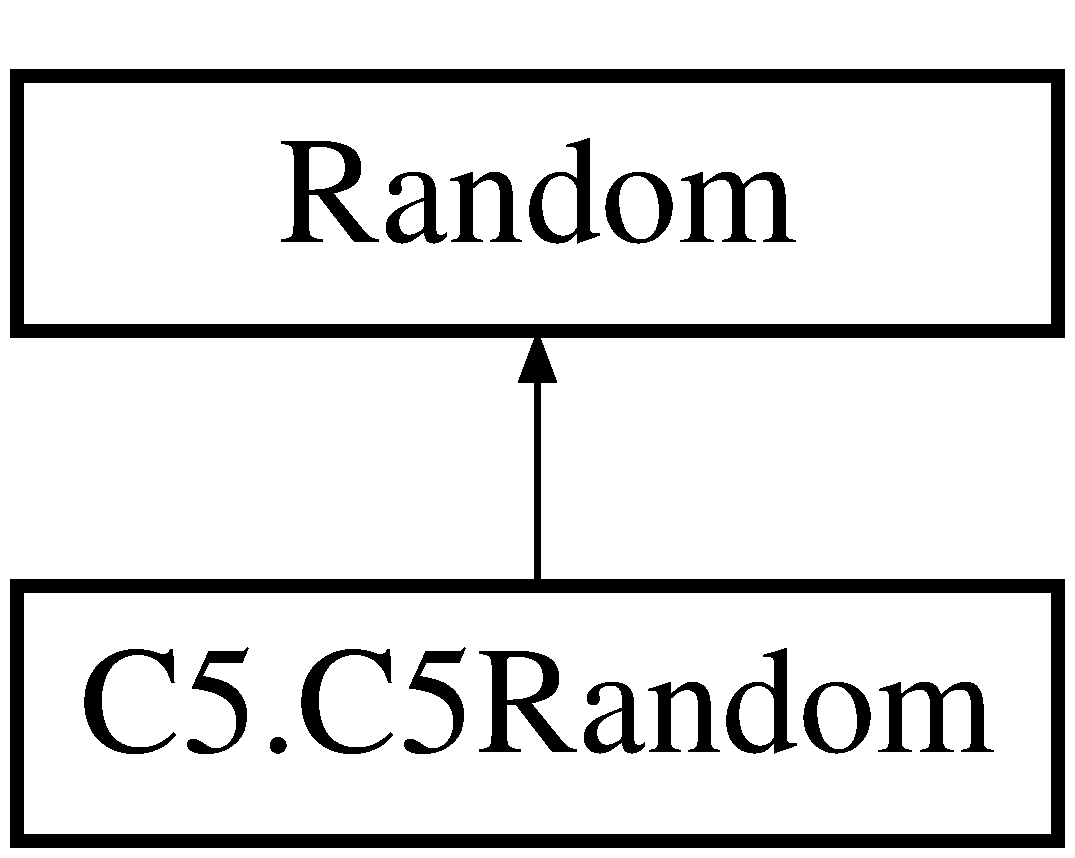
\includegraphics[height=2.000000cm]{class_c5_1_1_c5_random}
\end{center}
\end{figure}
\subsection*{Public Member Functions}
\begin{DoxyCompactItemize}
\item 
override double \hyperlink{class_c5_1_1_c5_random_a66b68b6fb6e91c24b0a433bac84026e3}{Next\+Double} ()
\begin{DoxyCompactList}\small\item\em Get a new random System.\+Double value \end{DoxyCompactList}\item 
override int \hyperlink{class_c5_1_1_c5_random_a7e0b80136c433144428ac57b3381d14d}{Next} ()
\begin{DoxyCompactList}\small\item\em Get a new random System.\+Int32 value \end{DoxyCompactList}\item 
override int \hyperlink{class_c5_1_1_c5_random_af68b5b18966783cb717d6ca9835d9575}{Next} (int max)
\begin{DoxyCompactList}\small\item\em Get a random non-\/negative integer less than a given upper bound \end{DoxyCompactList}\item 
override int \hyperlink{class_c5_1_1_c5_random_a0c8d4a67fb32149cdf58a61466d40ca8}{Next} (int min, int max)
\begin{DoxyCompactList}\small\item\em Get a random integer between two given bounds \end{DoxyCompactList}\item 
override void \hyperlink{class_c5_1_1_c5_random_af55415fd511db1e7741d34cdc7fb781f}{Next\+Bytes} (byte\mbox{[}$\,$\mbox{]} buffer)
\begin{DoxyCompactList}\small\item\em Fill a array of byte with random bytes \end{DoxyCompactList}\item 
\hyperlink{class_c5_1_1_c5_random_aad64b2b20feaac43d6d6571a22091554}{C5\+Random} ()
\begin{DoxyCompactList}\small\item\em Create a random number generator seed by system time. \end{DoxyCompactList}\item 
\hyperlink{class_c5_1_1_c5_random_a62b56d23ccf63e06ad79cfe4d2da1f41}{C5\+Random} (long seed)
\begin{DoxyCompactList}\small\item\em Create a random number generator with a given seed \end{DoxyCompactList}\item 
\hyperlink{class_c5_1_1_c5_random_a55c96d1007edceb65149cca9793405f6}{C5\+Random} (uint\mbox{[}$\,$\mbox{]} Q)
\begin{DoxyCompactList}\small\item\em Create a random number generator with a specified internal start state. \end{DoxyCompactList}\end{DoxyCompactItemize}
\subsection*{Protected Member Functions}
\begin{DoxyCompactItemize}
\item 
override double \hyperlink{class_c5_1_1_c5_random_aaa4ee7bc01657c6dacc68da89b8f7036}{Sample} ()
\begin{DoxyCompactList}\small\item\em Get a new random System.\+Double value \end{DoxyCompactList}\end{DoxyCompactItemize}


\subsection{Detailed Description}
A modern random number generator based on G. Marsaglia\+: Seeds for Random Number Generators, Communications of the A\+C\+M 46, 5 (May 2003) 90-\/93; and a posting by Marsaglia to comp.\+lang.\+c on 2003-\/04-\/03. 



\subsection{Constructor \& Destructor Documentation}
\hypertarget{class_c5_1_1_c5_random_aad64b2b20feaac43d6d6571a22091554}{}\index{C5\+::\+C5\+Random@{C5\+::\+C5\+Random}!C5\+Random@{C5\+Random}}
\index{C5\+Random@{C5\+Random}!C5\+::\+C5\+Random@{C5\+::\+C5\+Random}}
\subsubsection[{C5\+Random()}]{\setlength{\rightskip}{0pt plus 5cm}C5.\+C5\+Random.\+C5\+Random (
\begin{DoxyParamCaption}
{}
\end{DoxyParamCaption}
)}\label{class_c5_1_1_c5_random_aad64b2b20feaac43d6d6571a22091554}


Create a random number generator seed by system time. 

\hypertarget{class_c5_1_1_c5_random_a62b56d23ccf63e06ad79cfe4d2da1f41}{}\index{C5\+::\+C5\+Random@{C5\+::\+C5\+Random}!C5\+Random@{C5\+Random}}
\index{C5\+Random@{C5\+Random}!C5\+::\+C5\+Random@{C5\+::\+C5\+Random}}
\subsubsection[{C5\+Random(long seed)}]{\setlength{\rightskip}{0pt plus 5cm}C5.\+C5\+Random.\+C5\+Random (
\begin{DoxyParamCaption}
\item[{long}]{seed}
\end{DoxyParamCaption}
)}\label{class_c5_1_1_c5_random_a62b56d23ccf63e06ad79cfe4d2da1f41}


Create a random number generator with a given seed 


\begin{DoxyExceptions}{Exceptions}
{\em Argument\+Exception} & If seed is zero\\
\hline
\end{DoxyExceptions}

\begin{DoxyParams}{Parameters}
{\em seed} & The seed\\
\hline
\end{DoxyParams}
\hypertarget{class_c5_1_1_c5_random_a55c96d1007edceb65149cca9793405f6}{}\index{C5\+::\+C5\+Random@{C5\+::\+C5\+Random}!C5\+Random@{C5\+Random}}
\index{C5\+Random@{C5\+Random}!C5\+::\+C5\+Random@{C5\+::\+C5\+Random}}
\subsubsection[{C5\+Random(uint[] Q)}]{\setlength{\rightskip}{0pt plus 5cm}C5.\+C5\+Random.\+C5\+Random (
\begin{DoxyParamCaption}
\item[{uint\mbox{[}$\,$\mbox{]}}]{Q}
\end{DoxyParamCaption}
)}\label{class_c5_1_1_c5_random_a55c96d1007edceb65149cca9793405f6}


Create a random number generator with a specified internal start state. 


\begin{DoxyExceptions}{Exceptions}
{\em Argument\+Exception} & If Q is not of length exactly 16\\
\hline
\end{DoxyExceptions}

\begin{DoxyParams}{Parameters}
{\em Q} & The start state. Must be a collection of random bits given by an array of exactly 16 uints.\\
\hline
\end{DoxyParams}


\subsection{Member Function Documentation}
\hypertarget{class_c5_1_1_c5_random_a7e0b80136c433144428ac57b3381d14d}{}\index{C5\+::\+C5\+Random@{C5\+::\+C5\+Random}!Next@{Next}}
\index{Next@{Next}!C5\+::\+C5\+Random@{C5\+::\+C5\+Random}}
\subsubsection[{Next()}]{\setlength{\rightskip}{0pt plus 5cm}override int C5.\+C5\+Random.\+Next (
\begin{DoxyParamCaption}
{}
\end{DoxyParamCaption}
)}\label{class_c5_1_1_c5_random_a7e0b80136c433144428ac57b3381d14d}


Get a new random System.\+Int32 value 

\begin{DoxyReturn}{Returns}
The random int
\end{DoxyReturn}
\hypertarget{class_c5_1_1_c5_random_af68b5b18966783cb717d6ca9835d9575}{}\index{C5\+::\+C5\+Random@{C5\+::\+C5\+Random}!Next@{Next}}
\index{Next@{Next}!C5\+::\+C5\+Random@{C5\+::\+C5\+Random}}
\subsubsection[{Next(int max)}]{\setlength{\rightskip}{0pt plus 5cm}override int C5.\+C5\+Random.\+Next (
\begin{DoxyParamCaption}
\item[{int}]{max}
\end{DoxyParamCaption}
)}\label{class_c5_1_1_c5_random_af68b5b18966783cb717d6ca9835d9575}


Get a random non-\/negative integer less than a given upper bound 


\begin{DoxyExceptions}{Exceptions}
{\em Argument\+Exception} & If max is negative\\
\hline
\end{DoxyExceptions}

\begin{DoxyParams}{Parameters}
{\em max} & The upper bound (exclusive)\\
\hline
\end{DoxyParams}
\begin{DoxyReturn}{Returns}

\end{DoxyReturn}
\hypertarget{class_c5_1_1_c5_random_a0c8d4a67fb32149cdf58a61466d40ca8}{}\index{C5\+::\+C5\+Random@{C5\+::\+C5\+Random}!Next@{Next}}
\index{Next@{Next}!C5\+::\+C5\+Random@{C5\+::\+C5\+Random}}
\subsubsection[{Next(int min, int max)}]{\setlength{\rightskip}{0pt plus 5cm}override int C5.\+C5\+Random.\+Next (
\begin{DoxyParamCaption}
\item[{int}]{min, }
\item[{int}]{max}
\end{DoxyParamCaption}
)}\label{class_c5_1_1_c5_random_a0c8d4a67fb32149cdf58a61466d40ca8}


Get a random integer between two given bounds 


\begin{DoxyExceptions}{Exceptions}
{\em Argument\+Exception} & If max is less than min\\
\hline
\end{DoxyExceptions}

\begin{DoxyParams}{Parameters}
{\em min} & The lower bound (inclusive)\\
\hline
{\em max} & The upper bound (exclusive)\\
\hline
\end{DoxyParams}
\begin{DoxyReturn}{Returns}

\end{DoxyReturn}
\hypertarget{class_c5_1_1_c5_random_af55415fd511db1e7741d34cdc7fb781f}{}\index{C5\+::\+C5\+Random@{C5\+::\+C5\+Random}!Next\+Bytes@{Next\+Bytes}}
\index{Next\+Bytes@{Next\+Bytes}!C5\+::\+C5\+Random@{C5\+::\+C5\+Random}}
\subsubsection[{Next\+Bytes(byte[] buffer)}]{\setlength{\rightskip}{0pt plus 5cm}override void C5.\+C5\+Random.\+Next\+Bytes (
\begin{DoxyParamCaption}
\item[{byte\mbox{[}$\,$\mbox{]}}]{buffer}
\end{DoxyParamCaption}
)}\label{class_c5_1_1_c5_random_af55415fd511db1e7741d34cdc7fb781f}


Fill a array of byte with random bytes 


\begin{DoxyParams}{Parameters}
{\em buffer} & The array to fill\\
\hline
\end{DoxyParams}
\hypertarget{class_c5_1_1_c5_random_a66b68b6fb6e91c24b0a433bac84026e3}{}\index{C5\+::\+C5\+Random@{C5\+::\+C5\+Random}!Next\+Double@{Next\+Double}}
\index{Next\+Double@{Next\+Double}!C5\+::\+C5\+Random@{C5\+::\+C5\+Random}}
\subsubsection[{Next\+Double()}]{\setlength{\rightskip}{0pt plus 5cm}override double C5.\+C5\+Random.\+Next\+Double (
\begin{DoxyParamCaption}
{}
\end{DoxyParamCaption}
)}\label{class_c5_1_1_c5_random_a66b68b6fb6e91c24b0a433bac84026e3}


Get a new random System.\+Double value 

\begin{DoxyReturn}{Returns}
The random double
\end{DoxyReturn}
\hypertarget{class_c5_1_1_c5_random_aaa4ee7bc01657c6dacc68da89b8f7036}{}\index{C5\+::\+C5\+Random@{C5\+::\+C5\+Random}!Sample@{Sample}}
\index{Sample@{Sample}!C5\+::\+C5\+Random@{C5\+::\+C5\+Random}}
\subsubsection[{Sample()}]{\setlength{\rightskip}{0pt plus 5cm}override double C5.\+C5\+Random.\+Sample (
\begin{DoxyParamCaption}
{}
\end{DoxyParamCaption}
)\hspace{0.3cm}{\ttfamily [protected]}}\label{class_c5_1_1_c5_random_aaa4ee7bc01657c6dacc68da89b8f7036}


Get a new random System.\+Double value 

\begin{DoxyReturn}{Returns}
The random double
\end{DoxyReturn}


The documentation for this class was generated from the following file\+:\begin{DoxyCompactItemize}
\item 
C\+:/\+Users/rasmusl/\+Source/\+Repos/\+C5/\+C5/\hyperlink{_random_8cs}{Random.\+cs}\end{DoxyCompactItemize}

\hypertarget{class_c5_1_1_circular_queue}{}\section{C5.\+Circular\+Queue$<$ T $>$ Class Template Reference}
\label{class_c5_1_1_circular_queue}\index{C5.\+Circular\+Queue$<$ T $>$@{C5.\+Circular\+Queue$<$ T $>$}}


 


Inheritance diagram for C5.\+Circular\+Queue$<$ T $>$\+:\begin{figure}[H]
\begin{center}
\leavevmode
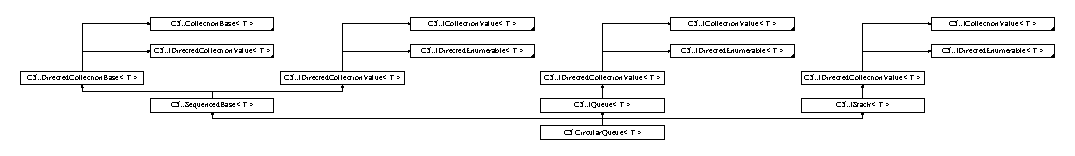
\includegraphics[height=1.643193cm]{class_c5_1_1_circular_queue}
\end{center}
\end{figure}
\subsection*{Public Member Functions}
\begin{DoxyCompactItemize}
\item 
\hyperlink{class_c5_1_1_circular_queue_a8b23dc95a35d343c2d6a745ebb812090}{Circular\+Queue} ()
\item 
\hyperlink{class_c5_1_1_circular_queue_a7b0161842b7ffcd9309257cf6e11a205}{Circular\+Queue} (int capacity)
\item 
virtual void \hyperlink{class_c5_1_1_circular_queue_a38228eb467c6366bbdfe930af2a6a3f7}{Enqueue} (T item)
\item 
virtual T \hyperlink{class_c5_1_1_circular_queue_ad52b370d4ab23656feeeeddf840da857}{Dequeue} ()
\item 
void \hyperlink{class_c5_1_1_circular_queue_a03b6cfbe23af1164ef4b68db24698ce7}{Push} (T item)
\item 
T \hyperlink{class_c5_1_1_circular_queue_a0a8d62216e8a17d072829f1c6214a262}{Pop} ()
\item 
override T \hyperlink{class_c5_1_1_circular_queue_aeabd2341783df834015d58b04c0c0a11}{Choose} ()
\item 
override S\+C\+G.\+I\+Enumerator$<$ T $>$ \hyperlink{class_c5_1_1_circular_queue_ae1ab5e745ced280db9b9a175a66dc5b4}{Get\+Enumerator} ()
\item 
override \hyperlink{interface_c5_1_1_i_directed_collection_value}{I\+Directed\+Collection\+Value}$<$ T $>$ \hyperlink{class_c5_1_1_circular_queue_a9df19a0a07cd854a59df4d3f976cf169}{Backwards} ()
\item 
virtual bool \hyperlink{class_c5_1_1_circular_queue_a57f406e63f6a7f41e9617933220e42a3}{Check} ()
\end{DoxyCompactItemize}
\subsection*{Properties}
\begin{DoxyCompactItemize}
\item 
override \hyperlink{namespace_c5_a9143bfd561fffa025d21561674758008}{Event\+Type\+Enum} \hyperlink{class_c5_1_1_circular_queue_a2dc39118f0d30f1bae7d3a73d4d2e4c6}{Listenable\+Events}\hspace{0.3cm}{\ttfamily  \mbox{[}get\mbox{]}}
\item 
virtual bool \hyperlink{class_c5_1_1_circular_queue_a0146f541106c3d6cf4259a1a6fe61d9c}{Allows\+Duplicates}\hspace{0.3cm}{\ttfamily  \mbox{[}get\mbox{]}}
\item 
virtual T \hyperlink{class_c5_1_1_circular_queue_a26b24b8ca3560860d09710dc8e8409bb}{this\mbox{[}int i\mbox{]}}\hspace{0.3cm}{\ttfamily  \mbox{[}get\mbox{]}}
\begin{DoxyCompactList}\small\item\em Get the i\textquotesingle{}th item in the queue. The front of the queue is at index 0. \end{DoxyCompactList}\end{DoxyCompactItemize}
\subsection*{Additional Inherited Members}


\subsection{Detailed Description}



\begin{DoxyTemplParams}{Template Parameters}
{\em T} & \\
\hline
\end{DoxyTemplParams}


\subsection{Constructor \& Destructor Documentation}
\hypertarget{class_c5_1_1_circular_queue_a8b23dc95a35d343c2d6a745ebb812090}{}\index{C5\+::\+Circular\+Queue@{C5\+::\+Circular\+Queue}!Circular\+Queue@{Circular\+Queue}}
\index{Circular\+Queue@{Circular\+Queue}!C5\+::\+Circular\+Queue@{C5\+::\+Circular\+Queue}}
\subsubsection[{Circular\+Queue()}]{\setlength{\rightskip}{0pt plus 5cm}{\bf C5.\+Circular\+Queue}$<$ T $>$.{\bf Circular\+Queue} (
\begin{DoxyParamCaption}
{}
\end{DoxyParamCaption}
)}\label{class_c5_1_1_circular_queue_a8b23dc95a35d343c2d6a745ebb812090}




\hypertarget{class_c5_1_1_circular_queue_a7b0161842b7ffcd9309257cf6e11a205}{}\index{C5\+::\+Circular\+Queue@{C5\+::\+Circular\+Queue}!Circular\+Queue@{Circular\+Queue}}
\index{Circular\+Queue@{Circular\+Queue}!C5\+::\+Circular\+Queue@{C5\+::\+Circular\+Queue}}
\subsubsection[{Circular\+Queue(int capacity)}]{\setlength{\rightskip}{0pt plus 5cm}{\bf C5.\+Circular\+Queue}$<$ T $>$.{\bf Circular\+Queue} (
\begin{DoxyParamCaption}
\item[{int}]{capacity}
\end{DoxyParamCaption}
)}\label{class_c5_1_1_circular_queue_a7b0161842b7ffcd9309257cf6e11a205}





\begin{DoxyParams}{Parameters}
{\em capacity} & \\
\hline
\end{DoxyParams}


\subsection{Member Function Documentation}
\hypertarget{class_c5_1_1_circular_queue_a9df19a0a07cd854a59df4d3f976cf169}{}\index{C5\+::\+Circular\+Queue@{C5\+::\+Circular\+Queue}!Backwards@{Backwards}}
\index{Backwards@{Backwards}!C5\+::\+Circular\+Queue@{C5\+::\+Circular\+Queue}}
\subsubsection[{Backwards()}]{\setlength{\rightskip}{0pt plus 5cm}override {\bf I\+Directed\+Collection\+Value}$<$T$>$ {\bf C5.\+Circular\+Queue}$<$ T $>$.Backwards (
\begin{DoxyParamCaption}
{}
\end{DoxyParamCaption}
)\hspace{0.3cm}{\ttfamily [virtual]}}\label{class_c5_1_1_circular_queue_a9df19a0a07cd854a59df4d3f976cf169}




\begin{DoxyReturn}{Returns}

\end{DoxyReturn}


Implements \hyperlink{class_c5_1_1_directed_collection_base_a9a4c7d6571ff7d78ea5adcb0d8264ff1}{C5.\+Directed\+Collection\+Base$<$ T $>$}.

\hypertarget{class_c5_1_1_circular_queue_a57f406e63f6a7f41e9617933220e42a3}{}\index{C5\+::\+Circular\+Queue@{C5\+::\+Circular\+Queue}!Check@{Check}}
\index{Check@{Check}!C5\+::\+Circular\+Queue@{C5\+::\+Circular\+Queue}}
\subsubsection[{Check()}]{\setlength{\rightskip}{0pt plus 5cm}virtual bool {\bf C5.\+Circular\+Queue}$<$ T $>$.Check (
\begin{DoxyParamCaption}
{}
\end{DoxyParamCaption}
)\hspace{0.3cm}{\ttfamily [virtual]}}\label{class_c5_1_1_circular_queue_a57f406e63f6a7f41e9617933220e42a3}




\begin{DoxyReturn}{Returns}

\end{DoxyReturn}
\hypertarget{class_c5_1_1_circular_queue_aeabd2341783df834015d58b04c0c0a11}{}\index{C5\+::\+Circular\+Queue@{C5\+::\+Circular\+Queue}!Choose@{Choose}}
\index{Choose@{Choose}!C5\+::\+Circular\+Queue@{C5\+::\+Circular\+Queue}}
\subsubsection[{Choose()}]{\setlength{\rightskip}{0pt plus 5cm}override T {\bf C5.\+Circular\+Queue}$<$ T $>$.Choose (
\begin{DoxyParamCaption}
{}
\end{DoxyParamCaption}
)}\label{class_c5_1_1_circular_queue_aeabd2341783df834015d58b04c0c0a11}




\begin{DoxyReturn}{Returns}

\end{DoxyReturn}


Implements \hyperlink{interface_c5_1_1_i_collection_value_af72d52ddd8ea4130d508e1cf020cf7eb}{C5.\+I\+Collection\+Value$<$ T $>$}.

\hypertarget{class_c5_1_1_circular_queue_ad52b370d4ab23656feeeeddf840da857}{}\index{C5\+::\+Circular\+Queue@{C5\+::\+Circular\+Queue}!Dequeue@{Dequeue}}
\index{Dequeue@{Dequeue}!C5\+::\+Circular\+Queue@{C5\+::\+Circular\+Queue}}
\subsubsection[{Dequeue()}]{\setlength{\rightskip}{0pt plus 5cm}virtual T {\bf C5.\+Circular\+Queue}$<$ T $>$.Dequeue (
\begin{DoxyParamCaption}
{}
\end{DoxyParamCaption}
)\hspace{0.3cm}{\ttfamily [virtual]}}\label{class_c5_1_1_circular_queue_ad52b370d4ab23656feeeeddf840da857}




\begin{DoxyReturn}{Returns}

\end{DoxyReturn}


Implements \hyperlink{interface_c5_1_1_i_queue_ae64bb24d3237ad9cef4f55593ca20bc7}{C5.\+I\+Queue$<$ T $>$}.

\hypertarget{class_c5_1_1_circular_queue_a38228eb467c6366bbdfe930af2a6a3f7}{}\index{C5\+::\+Circular\+Queue@{C5\+::\+Circular\+Queue}!Enqueue@{Enqueue}}
\index{Enqueue@{Enqueue}!C5\+::\+Circular\+Queue@{C5\+::\+Circular\+Queue}}
\subsubsection[{Enqueue(\+T item)}]{\setlength{\rightskip}{0pt plus 5cm}virtual void {\bf C5.\+Circular\+Queue}$<$ T $>$.Enqueue (
\begin{DoxyParamCaption}
\item[{T}]{item}
\end{DoxyParamCaption}
)\hspace{0.3cm}{\ttfamily [virtual]}}\label{class_c5_1_1_circular_queue_a38228eb467c6366bbdfe930af2a6a3f7}





\begin{DoxyParams}{Parameters}
{\em item} & \\
\hline
\end{DoxyParams}


Implements \hyperlink{interface_c5_1_1_i_queue_afceb820ca32b996f6fd5c34a85ccbacd}{C5.\+I\+Queue$<$ T $>$}.

\hypertarget{class_c5_1_1_circular_queue_ae1ab5e745ced280db9b9a175a66dc5b4}{}\index{C5\+::\+Circular\+Queue@{C5\+::\+Circular\+Queue}!Get\+Enumerator@{Get\+Enumerator}}
\index{Get\+Enumerator@{Get\+Enumerator}!C5\+::\+Circular\+Queue@{C5\+::\+Circular\+Queue}}
\subsubsection[{Get\+Enumerator()}]{\setlength{\rightskip}{0pt plus 5cm}override S\+C\+G.\+I\+Enumerator$<$T$>$ {\bf C5.\+Circular\+Queue}$<$ T $>$.Get\+Enumerator (
\begin{DoxyParamCaption}
{}
\end{DoxyParamCaption}
)\hspace{0.3cm}{\ttfamily [virtual]}}\label{class_c5_1_1_circular_queue_ae1ab5e745ced280db9b9a175a66dc5b4}




\begin{DoxyReturn}{Returns}

\end{DoxyReturn}


Implements \hyperlink{class_c5_1_1_sequenced_base_a07d117175b630fd7f87f6e61b05259dc}{C5.\+Sequenced\+Base$<$ T $>$}.

\hypertarget{class_c5_1_1_circular_queue_a0a8d62216e8a17d072829f1c6214a262}{}\index{C5\+::\+Circular\+Queue@{C5\+::\+Circular\+Queue}!Pop@{Pop}}
\index{Pop@{Pop}!C5\+::\+Circular\+Queue@{C5\+::\+Circular\+Queue}}
\subsubsection[{Pop()}]{\setlength{\rightskip}{0pt plus 5cm}T {\bf C5.\+Circular\+Queue}$<$ T $>$.Pop (
\begin{DoxyParamCaption}
{}
\end{DoxyParamCaption}
)}\label{class_c5_1_1_circular_queue_a0a8d62216e8a17d072829f1c6214a262}




\begin{DoxyReturn}{Returns}

\end{DoxyReturn}


Implements \hyperlink{interface_c5_1_1_i_stack_ad85678b4d9f9a1277b02d5913d0e1d55}{C5.\+I\+Stack$<$ T $>$}.

\hypertarget{class_c5_1_1_circular_queue_a03b6cfbe23af1164ef4b68db24698ce7}{}\index{C5\+::\+Circular\+Queue@{C5\+::\+Circular\+Queue}!Push@{Push}}
\index{Push@{Push}!C5\+::\+Circular\+Queue@{C5\+::\+Circular\+Queue}}
\subsubsection[{Push(\+T item)}]{\setlength{\rightskip}{0pt plus 5cm}void {\bf C5.\+Circular\+Queue}$<$ T $>$.Push (
\begin{DoxyParamCaption}
\item[{T}]{item}
\end{DoxyParamCaption}
)}\label{class_c5_1_1_circular_queue_a03b6cfbe23af1164ef4b68db24698ce7}





\begin{DoxyParams}{Parameters}
{\em item} & \\
\hline
\end{DoxyParams}


Implements \hyperlink{interface_c5_1_1_i_stack_a98462dd9cda5d818fc1bce6a5055f000}{C5.\+I\+Stack$<$ T $>$}.



\subsection{Property Documentation}
\hypertarget{class_c5_1_1_circular_queue_a0146f541106c3d6cf4259a1a6fe61d9c}{}\index{C5\+::\+Circular\+Queue@{C5\+::\+Circular\+Queue}!Allows\+Duplicates@{Allows\+Duplicates}}
\index{Allows\+Duplicates@{Allows\+Duplicates}!C5\+::\+Circular\+Queue@{C5\+::\+Circular\+Queue}}
\subsubsection[{Allows\+Duplicates}]{\setlength{\rightskip}{0pt plus 5cm}virtual bool {\bf C5.\+Circular\+Queue}$<$ T $>$.Allows\+Duplicates\hspace{0.3cm}{\ttfamily [get]}}\label{class_c5_1_1_circular_queue_a0146f541106c3d6cf4259a1a6fe61d9c}




\hypertarget{class_c5_1_1_circular_queue_a2dc39118f0d30f1bae7d3a73d4d2e4c6}{}\index{C5\+::\+Circular\+Queue@{C5\+::\+Circular\+Queue}!Listenable\+Events@{Listenable\+Events}}
\index{Listenable\+Events@{Listenable\+Events}!C5\+::\+Circular\+Queue@{C5\+::\+Circular\+Queue}}
\subsubsection[{Listenable\+Events}]{\setlength{\rightskip}{0pt plus 5cm}override {\bf Event\+Type\+Enum} {\bf C5.\+Circular\+Queue}$<$ T $>$.Listenable\+Events\hspace{0.3cm}{\ttfamily [get]}}\label{class_c5_1_1_circular_queue_a2dc39118f0d30f1bae7d3a73d4d2e4c6}




\hypertarget{class_c5_1_1_circular_queue_a26b24b8ca3560860d09710dc8e8409bb}{}\index{C5\+::\+Circular\+Queue@{C5\+::\+Circular\+Queue}!this\mbox{[}int i\mbox{]}@{this[int i]}}
\index{this\mbox{[}int i\mbox{]}@{this[int i]}!C5\+::\+Circular\+Queue@{C5\+::\+Circular\+Queue}}
\subsubsection[{this[int i]}]{\setlength{\rightskip}{0pt plus 5cm}virtual T {\bf C5.\+Circular\+Queue}$<$ T $>$.this\mbox{[}int i\mbox{]}\hspace{0.3cm}{\ttfamily [get]}}\label{class_c5_1_1_circular_queue_a26b24b8ca3560860d09710dc8e8409bb}


Get the i\textquotesingle{}th item in the queue. The front of the queue is at index 0. 


\begin{DoxyParams}{Parameters}
{\em i} & \\
\hline
\end{DoxyParams}
\begin{DoxyReturn}{Returns}

\end{DoxyReturn}


The documentation for this class was generated from the following file\+:\begin{DoxyCompactItemize}
\item 
C\+:/\+Users/rasmusl/\+Source/\+Repos/\+C5/\+C5/arrays/\hyperlink{_circular_queue_8cs}{Circular\+Queue.\+cs}\end{DoxyCompactItemize}

\hypertarget{class_c5_1_1_cleared_event_args}{}\section{C5.\+Cleared\+Event\+Args Class Reference}
\label{class_c5_1_1_cleared_event_args}\index{C5.\+Cleared\+Event\+Args@{C5.\+Cleared\+Event\+Args}}


 


Inheritance diagram for C5.\+Cleared\+Event\+Args\+:\begin{figure}[H]
\begin{center}
\leavevmode
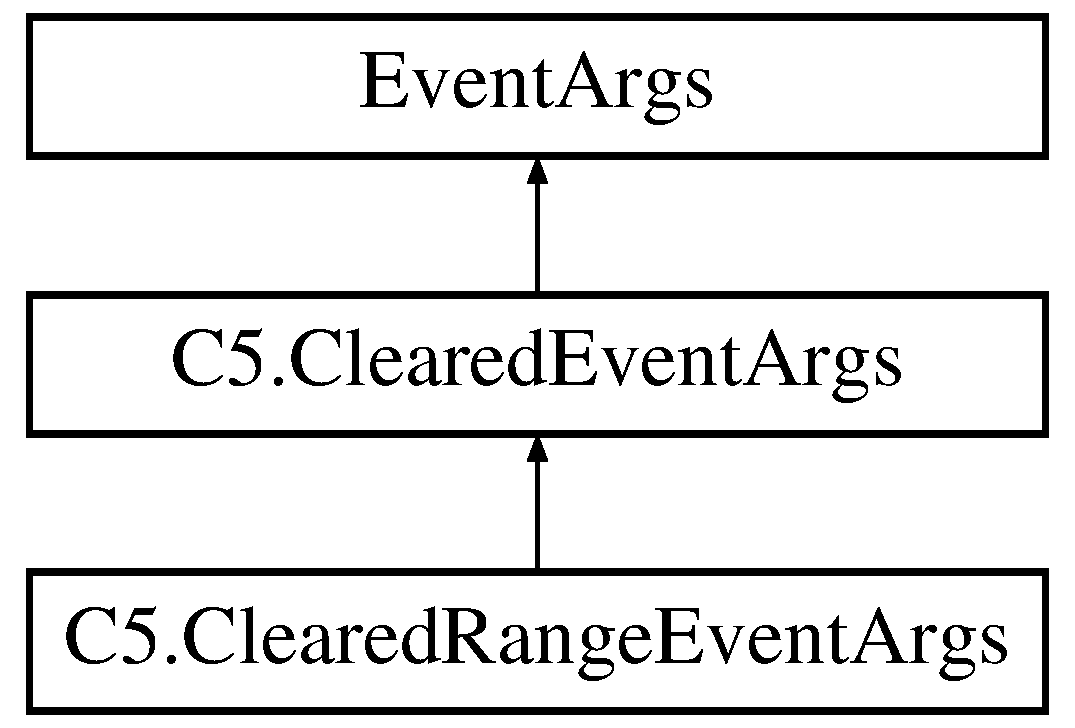
\includegraphics[height=3.000000cm]{class_c5_1_1_cleared_event_args}
\end{center}
\end{figure}
\subsection*{Public Member Functions}
\begin{DoxyCompactItemize}
\item 
\hyperlink{class_c5_1_1_cleared_event_args_a5415fd8bfed551c7677984ec09395f44}{Cleared\+Event\+Args} (bool full, int count)
\item 
override string \hyperlink{class_c5_1_1_cleared_event_args_a01ef1a40e119365d8ff23c3d72602db9}{To\+String} ()
\end{DoxyCompactItemize}
\subsection*{Public Attributes}
\begin{DoxyCompactItemize}
\item 
readonly bool \hyperlink{class_c5_1_1_cleared_event_args_a2f772af2802fb799370ee6d351cb6d0b}{Full}
\item 
readonly int \hyperlink{class_c5_1_1_cleared_event_args_a5a635819ba820b9d202786554d84f737}{Count}
\end{DoxyCompactItemize}


\subsection{Detailed Description}




\subsection{Constructor \& Destructor Documentation}
\hypertarget{class_c5_1_1_cleared_event_args_a5415fd8bfed551c7677984ec09395f44}{}\index{C5\+::\+Cleared\+Event\+Args@{C5\+::\+Cleared\+Event\+Args}!Cleared\+Event\+Args@{Cleared\+Event\+Args}}
\index{Cleared\+Event\+Args@{Cleared\+Event\+Args}!C5\+::\+Cleared\+Event\+Args@{C5\+::\+Cleared\+Event\+Args}}
\subsubsection[{Cleared\+Event\+Args(bool full, int count)}]{\setlength{\rightskip}{0pt plus 5cm}C5.\+Cleared\+Event\+Args.\+Cleared\+Event\+Args (
\begin{DoxyParamCaption}
\item[{bool}]{full, }
\item[{int}]{count}
\end{DoxyParamCaption}
)}\label{class_c5_1_1_cleared_event_args_a5415fd8bfed551c7677984ec09395f44}





\begin{DoxyParams}{Parameters}
{\em full} & True if the operation cleared all of the collection\\
\hline
{\em count} & The number of items removed by the clear.\\
\hline
\end{DoxyParams}


\subsection{Member Function Documentation}
\hypertarget{class_c5_1_1_cleared_event_args_a01ef1a40e119365d8ff23c3d72602db9}{}\index{C5\+::\+Cleared\+Event\+Args@{C5\+::\+Cleared\+Event\+Args}!To\+String@{To\+String}}
\index{To\+String@{To\+String}!C5\+::\+Cleared\+Event\+Args@{C5\+::\+Cleared\+Event\+Args}}
\subsubsection[{To\+String()}]{\setlength{\rightskip}{0pt plus 5cm}override string C5.\+Cleared\+Event\+Args.\+To\+String (
\begin{DoxyParamCaption}
{}
\end{DoxyParamCaption}
)}\label{class_c5_1_1_cleared_event_args_a01ef1a40e119365d8ff23c3d72602db9}




\begin{DoxyReturn}{Returns}

\end{DoxyReturn}


\subsection{Member Data Documentation}
\hypertarget{class_c5_1_1_cleared_event_args_a5a635819ba820b9d202786554d84f737}{}\index{C5\+::\+Cleared\+Event\+Args@{C5\+::\+Cleared\+Event\+Args}!Count@{Count}}
\index{Count@{Count}!C5\+::\+Cleared\+Event\+Args@{C5\+::\+Cleared\+Event\+Args}}
\subsubsection[{Count}]{\setlength{\rightskip}{0pt plus 5cm}readonly int C5.\+Cleared\+Event\+Args.\+Count}\label{class_c5_1_1_cleared_event_args_a5a635819ba820b9d202786554d84f737}




\hypertarget{class_c5_1_1_cleared_event_args_a2f772af2802fb799370ee6d351cb6d0b}{}\index{C5\+::\+Cleared\+Event\+Args@{C5\+::\+Cleared\+Event\+Args}!Full@{Full}}
\index{Full@{Full}!C5\+::\+Cleared\+Event\+Args@{C5\+::\+Cleared\+Event\+Args}}
\subsubsection[{Full}]{\setlength{\rightskip}{0pt plus 5cm}readonly bool C5.\+Cleared\+Event\+Args.\+Full}\label{class_c5_1_1_cleared_event_args_a2f772af2802fb799370ee6d351cb6d0b}






The documentation for this class was generated from the following file\+:\begin{DoxyCompactItemize}
\item 
C\+:/\+Users/rasmusl/\+Source/\+Repos/\+C5/\+C5/\hyperlink{_events_8cs}{Events.\+cs}\end{DoxyCompactItemize}

\hypertarget{class_c5_1_1_cleared_range_event_args}{}\section{C5.\+Cleared\+Range\+Event\+Args Class Reference}
\label{class_c5_1_1_cleared_range_event_args}\index{C5.\+Cleared\+Range\+Event\+Args@{C5.\+Cleared\+Range\+Event\+Args}}


 


Inheritance diagram for C5.\+Cleared\+Range\+Event\+Args\+:\begin{figure}[H]
\begin{center}
\leavevmode
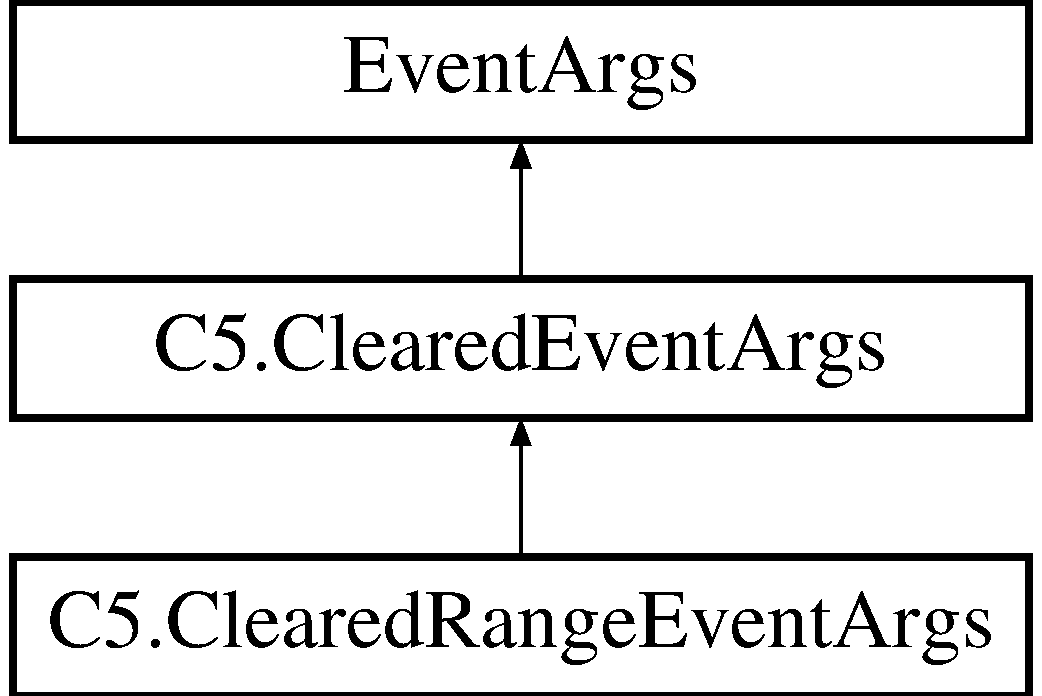
\includegraphics[height=3.000000cm]{class_c5_1_1_cleared_range_event_args}
\end{center}
\end{figure}
\subsection*{Public Member Functions}
\begin{DoxyCompactItemize}
\item 
\hyperlink{class_c5_1_1_cleared_range_event_args_ae8aeea017aa864f10471e070837dc908}{Cleared\+Range\+Event\+Args} (bool full, int count, int?start)
\item 
override string \hyperlink{class_c5_1_1_cleared_range_event_args_a1460b4c9431d78360945e1ce4d64864d}{To\+String} ()
\end{DoxyCompactItemize}
\subsection*{Public Attributes}
\begin{DoxyCompactItemize}
\item 
readonly int \hyperlink{class_c5_1_1_cleared_range_event_args_aa6c242b23ec6a07c3442a6c5b0cafd98}{Start}
\end{DoxyCompactItemize}


\subsection{Detailed Description}




\subsection{Constructor \& Destructor Documentation}
\hypertarget{class_c5_1_1_cleared_range_event_args_ae8aeea017aa864f10471e070837dc908}{}\index{C5\+::\+Cleared\+Range\+Event\+Args@{C5\+::\+Cleared\+Range\+Event\+Args}!Cleared\+Range\+Event\+Args@{Cleared\+Range\+Event\+Args}}
\index{Cleared\+Range\+Event\+Args@{Cleared\+Range\+Event\+Args}!C5\+::\+Cleared\+Range\+Event\+Args@{C5\+::\+Cleared\+Range\+Event\+Args}}
\subsubsection[{Cleared\+Range\+Event\+Args(bool full, int count, int?start)}]{\setlength{\rightskip}{0pt plus 5cm}C5.\+Cleared\+Range\+Event\+Args.\+Cleared\+Range\+Event\+Args (
\begin{DoxyParamCaption}
\item[{bool}]{full, }
\item[{int}]{count, }
\item[{int?}]{start}
\end{DoxyParamCaption}
)}\label{class_c5_1_1_cleared_range_event_args_ae8aeea017aa864f10471e070837dc908}





\begin{DoxyParams}{Parameters}
{\em full} & \\
\hline
{\em count} & \\
\hline
{\em start} & \\
\hline
\end{DoxyParams}


\subsection{Member Function Documentation}
\hypertarget{class_c5_1_1_cleared_range_event_args_a1460b4c9431d78360945e1ce4d64864d}{}\index{C5\+::\+Cleared\+Range\+Event\+Args@{C5\+::\+Cleared\+Range\+Event\+Args}!To\+String@{To\+String}}
\index{To\+String@{To\+String}!C5\+::\+Cleared\+Range\+Event\+Args@{C5\+::\+Cleared\+Range\+Event\+Args}}
\subsubsection[{To\+String()}]{\setlength{\rightskip}{0pt plus 5cm}override string C5.\+Cleared\+Range\+Event\+Args.\+To\+String (
\begin{DoxyParamCaption}
{}
\end{DoxyParamCaption}
)}\label{class_c5_1_1_cleared_range_event_args_a1460b4c9431d78360945e1ce4d64864d}




\begin{DoxyReturn}{Returns}

\end{DoxyReturn}


\subsection{Member Data Documentation}
\hypertarget{class_c5_1_1_cleared_range_event_args_aa6c242b23ec6a07c3442a6c5b0cafd98}{}\index{C5\+::\+Cleared\+Range\+Event\+Args@{C5\+::\+Cleared\+Range\+Event\+Args}!Start@{Start}}
\index{Start@{Start}!C5\+::\+Cleared\+Range\+Event\+Args@{C5\+::\+Cleared\+Range\+Event\+Args}}
\subsubsection[{Start}]{\setlength{\rightskip}{0pt plus 5cm}readonly int C5.\+Cleared\+Range\+Event\+Args.\+Start}\label{class_c5_1_1_cleared_range_event_args_aa6c242b23ec6a07c3442a6c5b0cafd98}






The documentation for this class was generated from the following file\+:\begin{DoxyCompactItemize}
\item 
C\+:/\+Users/rasmusl/\+Source/\+Repos/\+C5/\+C5/\hyperlink{_events_8cs}{Events.\+cs}\end{DoxyCompactItemize}

\hypertarget{class_c5_1_1_collection_base}{}\section{C5.\+Collection\+Base$<$ T $>$ Class Template Reference}
\label{class_c5_1_1_collection_base}\index{C5.\+Collection\+Base$<$ T $>$@{C5.\+Collection\+Base$<$ T $>$}}


Base class (abstract) for \hyperlink{interface_c5_1_1_i_collection}{I\+Collection} implementations.  


Inheritance diagram for C5.\+Collection\+Base$<$ T $>$\+:\begin{figure}[H]
\begin{center}
\leavevmode
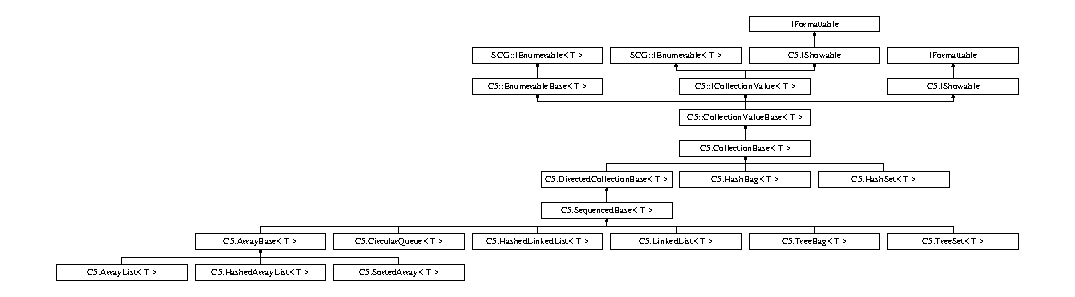
\includegraphics[height=3.546798cm]{class_c5_1_1_collection_base}
\end{center}
\end{figure}
\subsection*{Public Member Functions}
\begin{DoxyCompactItemize}
\item 
virtual int \hyperlink{class_c5_1_1_collection_base_a165f2e0e454cdd3d02c632afd44e0f0f}{Get\+Unsequenced\+Hash\+Code} ()
\begin{DoxyCompactList}\small\item\em Get the unsequenced collection hash code of this collection\+: from the cached value if present and up to date, else (re)compute. \end{DoxyCompactList}\item 
virtual bool \hyperlink{class_c5_1_1_collection_base_aacf42049e95f0bb781fcb1be9c3142a8}{Unsequenced\+Equals} (\hyperlink{interface_c5_1_1_i_collection}{I\+Collection}$<$ T $>$ other\+Collection)
\begin{DoxyCompactList}\small\item\em Check if the contents of other\+Collection is equal to the contents of this in the unsequenced sense. Uses the item equality comparer of this collection \end{DoxyCompactList}\item 
abstract override S\+C\+G.\+I\+Enumerator$<$ T $>$ \hyperlink{class_c5_1_1_collection_base_a3b4b98e2606afecb948019412c4c2533}{Get\+Enumerator} ()
\begin{DoxyCompactList}\small\item\em Create an enumerator for this collection. \end{DoxyCompactList}\end{DoxyCompactItemize}
\subsection*{Static Public Member Functions}
\begin{DoxyCompactItemize}
\item 
static int \hyperlink{class_c5_1_1_collection_base_ace9e9e72f14e465b9db074a539a80079}{Compute\+Hash\+Code} (\hyperlink{interface_c5_1_1_i_collection_value}{I\+Collection\+Value}$<$ T $>$ items, S\+C\+G.\+I\+Equality\+Comparer$<$ T $>$ \hyperlink{class_c5_1_1_collection_base_a95e343400be0e8f3f8d6310f1aaf2cc6}{itemequality\+Comparer})
\begin{DoxyCompactList}\small\item\em Compute the unsequenced hash code of a collection \end{DoxyCompactList}\item 
static bool \hyperlink{class_c5_1_1_collection_base_a2c019fdab3aee23b89421b4080b3cb9f}{Static\+Equals} (\hyperlink{interface_c5_1_1_i_collection}{I\+Collection}$<$ T $>$ collection1, \hyperlink{interface_c5_1_1_i_collection}{I\+Collection}$<$ T $>$ collection2, S\+C\+G.\+I\+Equality\+Comparer$<$ T $>$ \hyperlink{class_c5_1_1_collection_base_a95e343400be0e8f3f8d6310f1aaf2cc6}{itemequality\+Comparer})
\begin{DoxyCompactList}\small\item\em Examine if collection1 and collection2 are equal as unsequenced collections using the specified item equality\+Comparer (assumed compatible with the two collections). \end{DoxyCompactList}\end{DoxyCompactItemize}
\subsection*{Protected Member Functions}
\begin{DoxyCompactItemize}
\item 
\hyperlink{class_c5_1_1_collection_base_a30a3c7a3e0ce42c2f768db2788657dc5}{Collection\+Base} (S\+C\+G.\+I\+Equality\+Comparer$<$ T $>$ \hyperlink{class_c5_1_1_collection_base_a95e343400be0e8f3f8d6310f1aaf2cc6}{itemequality\+Comparer})
\item 
void \hyperlink{class_c5_1_1_collection_base_a65fdbed19443252a87929df9550fa126}{check\+Range} (int start, int count)
\begin{DoxyCompactList}\small\item\em Utility method for range checking. \end{DoxyCompactList}\item 
virtual void \hyperlink{class_c5_1_1_collection_base_a526ecabb3f13a4bbaf0ad35625c71666}{modifycheck} (int thestamp)
\begin{DoxyCompactList}\small\item\em Check if the collection has been modified since a specified time, expressed as a stamp value. \end{DoxyCompactList}\item 
virtual void \hyperlink{class_c5_1_1_collection_base_a99366c35ef7e0c9ec293110a54821e3c}{updatecheck} ()
\begin{DoxyCompactList}\small\item\em Check if it is valid to perform update operations, and if so increment stamp. \end{DoxyCompactList}\end{DoxyCompactItemize}
\subsection*{Protected Attributes}
\begin{DoxyCompactItemize}
\item 
bool \hyperlink{class_c5_1_1_collection_base_ae603bb5742908edb4871693723d0deda}{is\+Read\+Only\+Base} = false
\begin{DoxyCompactList}\small\item\em The underlying field of the Read\+Only property \end{DoxyCompactList}\item 
int \hyperlink{class_c5_1_1_collection_base_ae13bd5b482306a49a4d10654a9b8b064}{stamp}
\begin{DoxyCompactList}\small\item\em The current stamp value \end{DoxyCompactList}\item 
int \hyperlink{class_c5_1_1_collection_base_ab524b118754a5a8290b6528511272833}{size}
\begin{DoxyCompactList}\small\item\em The number of items in the collection \end{DoxyCompactList}\item 
readonly S\+C\+G.\+I\+Equality\+Comparer$<$ T $>$ \hyperlink{class_c5_1_1_collection_base_a95e343400be0e8f3f8d6310f1aaf2cc6}{itemequality\+Comparer}
\begin{DoxyCompactList}\small\item\em The item equality\+Comparer of the collection \end{DoxyCompactList}\end{DoxyCompactItemize}
\subsection*{Properties}
\begin{DoxyCompactItemize}
\item 
virtual bool \hyperlink{class_c5_1_1_collection_base_a4f9fea0df76b43f0c705fbc79a891bb9}{Is\+Read\+Only}\hspace{0.3cm}{\ttfamily  \mbox{[}get\mbox{]}}
\item 
override int \hyperlink{class_c5_1_1_collection_base_abd3c5c23faf3d44196d125676ae03039}{Count}\hspace{0.3cm}{\ttfamily  \mbox{[}get\mbox{]}}
\item 
override \hyperlink{namespace_c5_a615ba88dcdaa8d5a3c5f833a73d7fad6}{Speed} \hyperlink{class_c5_1_1_collection_base_a2c5361c8da79a23905c1730bb3cfce5b}{Count\+Speed}\hspace{0.3cm}{\ttfamily  \mbox{[}get\mbox{]}}
\begin{DoxyCompactList}\small\item\em The value is symbolic indicating the type of asymptotic complexity in terms of the size of this collection (worst-\/case or amortized as relevant). \end{DoxyCompactList}\item 
virtual S\+C\+G.\+I\+Equality\+Comparer$<$ T $>$ \hyperlink{class_c5_1_1_collection_base_ab3c81e20f42c012d8ff6b5658889d108}{Equality\+Comparer}\hspace{0.3cm}{\ttfamily  \mbox{[}get\mbox{]}}
\item 
override bool \hyperlink{class_c5_1_1_collection_base_a28a325cf904f11def90daf27c98007f6}{Is\+Empty}\hspace{0.3cm}{\ttfamily  \mbox{[}get\mbox{]}}
\end{DoxyCompactItemize}
\subsection*{Additional Inherited Members}


\subsection{Detailed Description}
Base class (abstract) for \hyperlink{interface_c5_1_1_i_collection}{I\+Collection} implementations. 



\subsection{Constructor \& Destructor Documentation}
\hypertarget{class_c5_1_1_collection_base_a30a3c7a3e0ce42c2f768db2788657dc5}{}\index{C5\+::\+Collection\+Base@{C5\+::\+Collection\+Base}!Collection\+Base@{Collection\+Base}}
\index{Collection\+Base@{Collection\+Base}!C5\+::\+Collection\+Base@{C5\+::\+Collection\+Base}}
\subsubsection[{Collection\+Base(\+S\+C\+G.\+I\+Equality\+Comparer$<$ T $>$ itemequality\+Comparer)}]{\setlength{\rightskip}{0pt plus 5cm}{\bf C5.\+Collection\+Base}$<$ T $>$.{\bf Collection\+Base} (
\begin{DoxyParamCaption}
\item[{S\+C\+G.\+I\+Equality\+Comparer$<$ T $>$}]{itemequality\+Comparer}
\end{DoxyParamCaption}
)\hspace{0.3cm}{\ttfamily [protected]}}\label{class_c5_1_1_collection_base_a30a3c7a3e0ce42c2f768db2788657dc5}





\begin{DoxyParams}{Parameters}
{\em itemequality\+Comparer} & \\
\hline
\end{DoxyParams}


\subsection{Member Function Documentation}
\hypertarget{class_c5_1_1_collection_base_a65fdbed19443252a87929df9550fa126}{}\index{C5\+::\+Collection\+Base@{C5\+::\+Collection\+Base}!check\+Range@{check\+Range}}
\index{check\+Range@{check\+Range}!C5\+::\+Collection\+Base@{C5\+::\+Collection\+Base}}
\subsubsection[{check\+Range(int start, int count)}]{\setlength{\rightskip}{0pt plus 5cm}void {\bf C5.\+Collection\+Base}$<$ T $>$.check\+Range (
\begin{DoxyParamCaption}
\item[{int}]{start, }
\item[{int}]{count}
\end{DoxyParamCaption}
)\hspace{0.3cm}{\ttfamily [protected]}}\label{class_c5_1_1_collection_base_a65fdbed19443252a87929df9550fa126}


Utility method for range checking. 


\begin{DoxyExceptions}{Exceptions}
{\em Argument\+Out\+Of\+Range\+Exception} & if the start or count is negative or if the range does not fit within collection size.\\
\hline
\end{DoxyExceptions}

\begin{DoxyParams}{Parameters}
{\em start} & start of range\\
\hline
{\em count} & size of range\\
\hline
\end{DoxyParams}
\hypertarget{class_c5_1_1_collection_base_ace9e9e72f14e465b9db074a539a80079}{}\index{C5\+::\+Collection\+Base@{C5\+::\+Collection\+Base}!Compute\+Hash\+Code@{Compute\+Hash\+Code}}
\index{Compute\+Hash\+Code@{Compute\+Hash\+Code}!C5\+::\+Collection\+Base@{C5\+::\+Collection\+Base}}
\subsubsection[{Compute\+Hash\+Code(\+I\+Collection\+Value$<$ T $>$ items, S\+C\+G.\+I\+Equality\+Comparer$<$ T $>$ itemequality\+Comparer)}]{\setlength{\rightskip}{0pt plus 5cm}static int {\bf C5.\+Collection\+Base}$<$ T $>$.Compute\+Hash\+Code (
\begin{DoxyParamCaption}
\item[{{\bf I\+Collection\+Value}$<$ T $>$}]{items, }
\item[{S\+C\+G.\+I\+Equality\+Comparer$<$ T $>$}]{itemequality\+Comparer}
\end{DoxyParamCaption}
)\hspace{0.3cm}{\ttfamily [static]}}\label{class_c5_1_1_collection_base_ace9e9e72f14e465b9db074a539a80079}


Compute the unsequenced hash code of a collection 


\begin{DoxyParams}{Parameters}
{\em items} & The collection to compute hash code for\\
\hline
{\em itemequality\+Comparer} & The item equality\+S\+C\+G.\+Comparer\\
\hline
\end{DoxyParams}
\begin{DoxyReturn}{Returns}
The hash code
\end{DoxyReturn}
\hypertarget{class_c5_1_1_collection_base_a3b4b98e2606afecb948019412c4c2533}{}\index{C5\+::\+Collection\+Base@{C5\+::\+Collection\+Base}!Get\+Enumerator@{Get\+Enumerator}}
\index{Get\+Enumerator@{Get\+Enumerator}!C5\+::\+Collection\+Base@{C5\+::\+Collection\+Base}}
\subsubsection[{Get\+Enumerator()}]{\setlength{\rightskip}{0pt plus 5cm}abstract override S\+C\+G.\+I\+Enumerator$<$T$>$ {\bf C5.\+Collection\+Base}$<$ T $>$.Get\+Enumerator (
\begin{DoxyParamCaption}
{}
\end{DoxyParamCaption}
)\hspace{0.3cm}{\ttfamily [pure virtual]}}\label{class_c5_1_1_collection_base_a3b4b98e2606afecb948019412c4c2533}


Create an enumerator for this collection. 

\begin{DoxyReturn}{Returns}
The enumerator
\end{DoxyReturn}


Implements \hyperlink{class_c5_1_1_collection_value_base_a0e8b891322ed9987a18f1a1ac87d2d4f}{C5.\+Collection\+Value\+Base$<$ T $>$}.



Implemented in \hyperlink{class_c5_1_1_hashed_linked_list_ae8f40668f13afb6cb05501446a3bcc4e}{C5.\+Hashed\+Linked\+List$<$ T $>$}, \hyperlink{class_c5_1_1_linked_list_ab23965434fba5e39a15eb4c0eb3c4901}{C5.\+Linked\+List$<$ T $>$}, \hyperlink{class_c5_1_1_hashed_array_list_a0ce81bee1c45ccbc3105698a4f4692a8}{C5.\+Hashed\+Array\+List$<$ T $>$}, \hyperlink{class_c5_1_1_array_list_ae6c2dc2f2aa8c9952d3267a37e9de01a}{C5.\+Array\+List$<$ T $>$}, \hyperlink{class_c5_1_1_array_base_a84a54c5fa039db32e27ca45c6b0cea85}{C5.\+Array\+Base$<$ T $>$}, \hyperlink{class_c5_1_1_sequenced_base_a07d117175b630fd7f87f6e61b05259dc}{C5.\+Sequenced\+Base$<$ T $>$}, \hyperlink{class_c5_1_1_hash_set_a4c404a22695abc0f6b47bf74d3d34034}{C5.\+Hash\+Set$<$ T $>$}, \hyperlink{class_c5_1_1_hash_bag_a621d77b2f8a7c3a826aace4be1d809b2}{C5.\+Hash\+Bag$<$ T $>$}, \hyperlink{class_c5_1_1_tree_bag_a2c00797c0e29dd52efa05f219b4c9c7e}{C5.\+Tree\+Bag$<$ T $>$}, \hyperlink{class_c5_1_1_tree_set_af9dd4aece1415276e1ede1ded6904179}{C5.\+Tree\+Set$<$ T $>$}, and \hyperlink{class_c5_1_1_circular_queue_ae1ab5e745ced280db9b9a175a66dc5b4}{C5.\+Circular\+Queue$<$ T $>$}.

\hypertarget{class_c5_1_1_collection_base_a165f2e0e454cdd3d02c632afd44e0f0f}{}\index{C5\+::\+Collection\+Base@{C5\+::\+Collection\+Base}!Get\+Unsequenced\+Hash\+Code@{Get\+Unsequenced\+Hash\+Code}}
\index{Get\+Unsequenced\+Hash\+Code@{Get\+Unsequenced\+Hash\+Code}!C5\+::\+Collection\+Base@{C5\+::\+Collection\+Base}}
\subsubsection[{Get\+Unsequenced\+Hash\+Code()}]{\setlength{\rightskip}{0pt plus 5cm}virtual int {\bf C5.\+Collection\+Base}$<$ T $>$.Get\+Unsequenced\+Hash\+Code (
\begin{DoxyParamCaption}
{}
\end{DoxyParamCaption}
)\hspace{0.3cm}{\ttfamily [virtual]}}\label{class_c5_1_1_collection_base_a165f2e0e454cdd3d02c632afd44e0f0f}


Get the unsequenced collection hash code of this collection\+: from the cached value if present and up to date, else (re)compute. 

\begin{DoxyReturn}{Returns}
The hash code
\end{DoxyReturn}


Reimplemented in \hyperlink{class_c5_1_1_hashed_linked_list_afa9c20b419017663841ffd613d31e75b}{C5.\+Hashed\+Linked\+List$<$ T $>$}, \hyperlink{class_c5_1_1_linked_list_a66dd343eb1edfd17074b200fccd59621}{C5.\+Linked\+List$<$ T $>$}, \hyperlink{class_c5_1_1_hashed_array_list_a8f23bbdc50d2c951e19fad0008f2f25a}{C5.\+Hashed\+Array\+List$<$ T $>$}, and \hyperlink{class_c5_1_1_array_list_a4f75d053012574e34e670597aa392e6f}{C5.\+Array\+List$<$ T $>$}.

\hypertarget{class_c5_1_1_collection_base_a526ecabb3f13a4bbaf0ad35625c71666}{}\index{C5\+::\+Collection\+Base@{C5\+::\+Collection\+Base}!modifycheck@{modifycheck}}
\index{modifycheck@{modifycheck}!C5\+::\+Collection\+Base@{C5\+::\+Collection\+Base}}
\subsubsection[{modifycheck(int thestamp)}]{\setlength{\rightskip}{0pt plus 5cm}virtual void {\bf C5.\+Collection\+Base}$<$ T $>$.modifycheck (
\begin{DoxyParamCaption}
\item[{int}]{thestamp}
\end{DoxyParamCaption}
)\hspace{0.3cm}{\ttfamily [protected]}, {\ttfamily [virtual]}}\label{class_c5_1_1_collection_base_a526ecabb3f13a4bbaf0ad35625c71666}


Check if the collection has been modified since a specified time, expressed as a stamp value. 


\begin{DoxyExceptions}{Exceptions}
{\em \hyperlink{class_c5_1_1_collection_modified_exception}{Collection\+Modified\+Exception}} & if this collection has been updated since a target time\\
\hline
\end{DoxyExceptions}

\begin{DoxyParams}{Parameters}
{\em thestamp} & The stamp identifying the target time\\
\hline
\end{DoxyParams}


Reimplemented in \hyperlink{class_c5_1_1_hashed_array_list_a0d8db9ef70c6d213b8c4f9302d9d1c15}{C5.\+Hashed\+Array\+List$<$ T $>$}, \hyperlink{class_c5_1_1_array_list_a1ab3f3702bc6ac270a421479e90437dd}{C5.\+Array\+List$<$ T $>$}, \hyperlink{class_c5_1_1_hashed_linked_list_a1e067df13f4f6b5f90753abf3db99ed7}{C5.\+Hashed\+Linked\+List$<$ T $>$}, and \hyperlink{class_c5_1_1_linked_list_aaba29831e0883a7bb02c5850a13323a7}{C5.\+Linked\+List$<$ T $>$}.

\hypertarget{class_c5_1_1_collection_base_a2c019fdab3aee23b89421b4080b3cb9f}{}\index{C5\+::\+Collection\+Base@{C5\+::\+Collection\+Base}!Static\+Equals@{Static\+Equals}}
\index{Static\+Equals@{Static\+Equals}!C5\+::\+Collection\+Base@{C5\+::\+Collection\+Base}}
\subsubsection[{Static\+Equals(\+I\+Collection$<$ T $>$ collection1, I\+Collection$<$ T $>$ collection2, S\+C\+G.\+I\+Equality\+Comparer$<$ T $>$ itemequality\+Comparer)}]{\setlength{\rightskip}{0pt plus 5cm}static bool {\bf C5.\+Collection\+Base}$<$ T $>$.Static\+Equals (
\begin{DoxyParamCaption}
\item[{{\bf I\+Collection}$<$ T $>$}]{collection1, }
\item[{{\bf I\+Collection}$<$ T $>$}]{collection2, }
\item[{S\+C\+G.\+I\+Equality\+Comparer$<$ T $>$}]{itemequality\+Comparer}
\end{DoxyParamCaption}
)\hspace{0.3cm}{\ttfamily [static]}}\label{class_c5_1_1_collection_base_a2c019fdab3aee23b89421b4080b3cb9f}


Examine if collection1 and collection2 are equal as unsequenced collections using the specified item equality\+Comparer (assumed compatible with the two collections). 


\begin{DoxyParams}{Parameters}
{\em collection1} & The first collection\\
\hline
{\em collection2} & The second collection\\
\hline
{\em itemequality\+Comparer} & The item equality\+Comparer to use for comparison\\
\hline
\end{DoxyParams}
\begin{DoxyReturn}{Returns}
True if equal
\end{DoxyReturn}
\hypertarget{class_c5_1_1_collection_base_aacf42049e95f0bb781fcb1be9c3142a8}{}\index{C5\+::\+Collection\+Base@{C5\+::\+Collection\+Base}!Unsequenced\+Equals@{Unsequenced\+Equals}}
\index{Unsequenced\+Equals@{Unsequenced\+Equals}!C5\+::\+Collection\+Base@{C5\+::\+Collection\+Base}}
\subsubsection[{Unsequenced\+Equals(\+I\+Collection$<$ T $>$ other\+Collection)}]{\setlength{\rightskip}{0pt plus 5cm}virtual bool {\bf C5.\+Collection\+Base}$<$ T $>$.Unsequenced\+Equals (
\begin{DoxyParamCaption}
\item[{{\bf I\+Collection}$<$ T $>$}]{other\+Collection}
\end{DoxyParamCaption}
)\hspace{0.3cm}{\ttfamily [virtual]}}\label{class_c5_1_1_collection_base_aacf42049e95f0bb781fcb1be9c3142a8}


Check if the contents of other\+Collection is equal to the contents of this in the unsequenced sense. Uses the item equality comparer of this collection 


\begin{DoxyParams}{Parameters}
{\em other\+Collection} & The collection to compare to.\\
\hline
\end{DoxyParams}
\begin{DoxyReturn}{Returns}
True if equal
\end{DoxyReturn}


Reimplemented in \hyperlink{class_c5_1_1_hashed_linked_list_a658a0145c6f1d28e00e558a705d3c8e2}{C5.\+Hashed\+Linked\+List$<$ T $>$}, \hyperlink{class_c5_1_1_linked_list_a5395d073fc0753d8842d805e28bda799}{C5.\+Linked\+List$<$ T $>$}, \hyperlink{class_c5_1_1_hashed_array_list_a6ed6c87e49b97c50d2cafba6fe050b26}{C5.\+Hashed\+Array\+List$<$ T $>$}, and \hyperlink{class_c5_1_1_array_list_a46753a14629243761d6056839747f23f}{C5.\+Array\+List$<$ T $>$}.

\hypertarget{class_c5_1_1_collection_base_a99366c35ef7e0c9ec293110a54821e3c}{}\index{C5\+::\+Collection\+Base@{C5\+::\+Collection\+Base}!updatecheck@{updatecheck}}
\index{updatecheck@{updatecheck}!C5\+::\+Collection\+Base@{C5\+::\+Collection\+Base}}
\subsubsection[{updatecheck()}]{\setlength{\rightskip}{0pt plus 5cm}virtual void {\bf C5.\+Collection\+Base}$<$ T $>$.updatecheck (
\begin{DoxyParamCaption}
{}
\end{DoxyParamCaption}
)\hspace{0.3cm}{\ttfamily [protected]}, {\ttfamily [virtual]}}\label{class_c5_1_1_collection_base_a99366c35ef7e0c9ec293110a54821e3c}


Check if it is valid to perform update operations, and if so increment stamp. 


\begin{DoxyExceptions}{Exceptions}
{\em \hyperlink{class_c5_1_1_read_only_collection_exception}{Read\+Only\+Collection\+Exception}} & If colection is read-\/only\\
\hline
\end{DoxyExceptions}


Reimplemented in \hyperlink{class_c5_1_1_hashed_array_list_a4a91454e022d105216e78756eff729c9}{C5.\+Hashed\+Array\+List$<$ T $>$}, \hyperlink{class_c5_1_1_array_list_a3d2755c3b8fdd5fc8d4b7b435a2002ff}{C5.\+Array\+List$<$ T $>$}, \hyperlink{class_c5_1_1_hashed_linked_list_af71c07992c8c580b5624734cbdd1bd4e}{C5.\+Hashed\+Linked\+List$<$ T $>$}, and \hyperlink{class_c5_1_1_linked_list_a1a74556032b0297634bda3f5e617e89d}{C5.\+Linked\+List$<$ T $>$}.



\subsection{Member Data Documentation}
\hypertarget{class_c5_1_1_collection_base_ae603bb5742908edb4871693723d0deda}{}\index{C5\+::\+Collection\+Base@{C5\+::\+Collection\+Base}!is\+Read\+Only\+Base@{is\+Read\+Only\+Base}}
\index{is\+Read\+Only\+Base@{is\+Read\+Only\+Base}!C5\+::\+Collection\+Base@{C5\+::\+Collection\+Base}}
\subsubsection[{is\+Read\+Only\+Base}]{\setlength{\rightskip}{0pt plus 5cm}bool {\bf C5.\+Collection\+Base}$<$ T $>$.is\+Read\+Only\+Base = false\hspace{0.3cm}{\ttfamily [protected]}}\label{class_c5_1_1_collection_base_ae603bb5742908edb4871693723d0deda}


The underlying field of the Read\+Only property 

\hypertarget{class_c5_1_1_collection_base_a95e343400be0e8f3f8d6310f1aaf2cc6}{}\index{C5\+::\+Collection\+Base@{C5\+::\+Collection\+Base}!itemequality\+Comparer@{itemequality\+Comparer}}
\index{itemequality\+Comparer@{itemequality\+Comparer}!C5\+::\+Collection\+Base@{C5\+::\+Collection\+Base}}
\subsubsection[{itemequality\+Comparer}]{\setlength{\rightskip}{0pt plus 5cm}readonly S\+C\+G.\+I\+Equality\+Comparer$<$T$>$ {\bf C5.\+Collection\+Base}$<$ T $>$.itemequality\+Comparer\hspace{0.3cm}{\ttfamily [protected]}}\label{class_c5_1_1_collection_base_a95e343400be0e8f3f8d6310f1aaf2cc6}


The item equality\+Comparer of the collection 

\hypertarget{class_c5_1_1_collection_base_ab524b118754a5a8290b6528511272833}{}\index{C5\+::\+Collection\+Base@{C5\+::\+Collection\+Base}!size@{size}}
\index{size@{size}!C5\+::\+Collection\+Base@{C5\+::\+Collection\+Base}}
\subsubsection[{size}]{\setlength{\rightskip}{0pt plus 5cm}int {\bf C5.\+Collection\+Base}$<$ T $>$.size\hspace{0.3cm}{\ttfamily [protected]}}\label{class_c5_1_1_collection_base_ab524b118754a5a8290b6528511272833}


The number of items in the collection 

\hypertarget{class_c5_1_1_collection_base_ae13bd5b482306a49a4d10654a9b8b064}{}\index{C5\+::\+Collection\+Base@{C5\+::\+Collection\+Base}!stamp@{stamp}}
\index{stamp@{stamp}!C5\+::\+Collection\+Base@{C5\+::\+Collection\+Base}}
\subsubsection[{stamp}]{\setlength{\rightskip}{0pt plus 5cm}int {\bf C5.\+Collection\+Base}$<$ T $>$.stamp\hspace{0.3cm}{\ttfamily [protected]}}\label{class_c5_1_1_collection_base_ae13bd5b482306a49a4d10654a9b8b064}


The current stamp value 



\subsection{Property Documentation}
\hypertarget{class_c5_1_1_collection_base_abd3c5c23faf3d44196d125676ae03039}{}\index{C5\+::\+Collection\+Base@{C5\+::\+Collection\+Base}!Count@{Count}}
\index{Count@{Count}!C5\+::\+Collection\+Base@{C5\+::\+Collection\+Base}}
\subsubsection[{Count}]{\setlength{\rightskip}{0pt plus 5cm}override int {\bf C5.\+Collection\+Base}$<$ T $>$.Count\hspace{0.3cm}{\ttfamily [get]}}\label{class_c5_1_1_collection_base_abd3c5c23faf3d44196d125676ae03039}




The size of this collection\hypertarget{class_c5_1_1_collection_base_a2c5361c8da79a23905c1730bb3cfce5b}{}\index{C5\+::\+Collection\+Base@{C5\+::\+Collection\+Base}!Count\+Speed@{Count\+Speed}}
\index{Count\+Speed@{Count\+Speed}!C5\+::\+Collection\+Base@{C5\+::\+Collection\+Base}}
\subsubsection[{Count\+Speed}]{\setlength{\rightskip}{0pt plus 5cm}override {\bf Speed} {\bf C5.\+Collection\+Base}$<$ T $>$.Count\+Speed\hspace{0.3cm}{\ttfamily [get]}}\label{class_c5_1_1_collection_base_a2c5361c8da79a23905c1730bb3cfce5b}


The value is symbolic indicating the type of asymptotic complexity in terms of the size of this collection (worst-\/case or amortized as relevant). 

A characterization of the speed of the {\ttfamily Count} property in this collection.\hypertarget{class_c5_1_1_collection_base_ab3c81e20f42c012d8ff6b5658889d108}{}\index{C5\+::\+Collection\+Base@{C5\+::\+Collection\+Base}!Equality\+Comparer@{Equality\+Comparer}}
\index{Equality\+Comparer@{Equality\+Comparer}!C5\+::\+Collection\+Base@{C5\+::\+Collection\+Base}}
\subsubsection[{Equality\+Comparer}]{\setlength{\rightskip}{0pt plus 5cm}virtual S\+C\+G.\+I\+Equality\+Comparer$<$T$>$ {\bf C5.\+Collection\+Base}$<$ T $>$.Equality\+Comparer\hspace{0.3cm}{\ttfamily [get]}}\label{class_c5_1_1_collection_base_ab3c81e20f42c012d8ff6b5658889d108}




\hypertarget{class_c5_1_1_collection_base_a28a325cf904f11def90daf27c98007f6}{}\index{C5\+::\+Collection\+Base@{C5\+::\+Collection\+Base}!Is\+Empty@{Is\+Empty}}
\index{Is\+Empty@{Is\+Empty}!C5\+::\+Collection\+Base@{C5\+::\+Collection\+Base}}
\subsubsection[{Is\+Empty}]{\setlength{\rightskip}{0pt plus 5cm}override bool {\bf C5.\+Collection\+Base}$<$ T $>$.Is\+Empty\hspace{0.3cm}{\ttfamily [get]}}\label{class_c5_1_1_collection_base_a28a325cf904f11def90daf27c98007f6}




True if this collection is empty\hypertarget{class_c5_1_1_collection_base_a4f9fea0df76b43f0c705fbc79a891bb9}{}\index{C5\+::\+Collection\+Base@{C5\+::\+Collection\+Base}!Is\+Read\+Only@{Is\+Read\+Only}}
\index{Is\+Read\+Only@{Is\+Read\+Only}!C5\+::\+Collection\+Base@{C5\+::\+Collection\+Base}}
\subsubsection[{Is\+Read\+Only}]{\setlength{\rightskip}{0pt plus 5cm}virtual bool {\bf C5.\+Collection\+Base}$<$ T $>$.Is\+Read\+Only\hspace{0.3cm}{\ttfamily [get]}}\label{class_c5_1_1_collection_base_a4f9fea0df76b43f0c705fbc79a891bb9}




True if this collection is read only

The documentation for this class was generated from the following file\+:\begin{DoxyCompactItemize}
\item 
C\+:/\+Users/rasmusl/\+Source/\+Repos/\+C5/\+C5/\hyperlink{_collections_8cs}{Collections.\+cs}\end{DoxyCompactItemize}

\hypertarget{class_c5_1_1_collection_modified_exception}{}\section{C5.\+Collection\+Modified\+Exception Class Reference}
\label{class_c5_1_1_collection_modified_exception}\index{C5.\+Collection\+Modified\+Exception@{C5.\+Collection\+Modified\+Exception}}


An exception thrown by enumerators, range views etc. when accessed after the underlying collection has been modified.  


Inheritance diagram for C5.\+Collection\+Modified\+Exception\+:\begin{figure}[H]
\begin{center}
\leavevmode
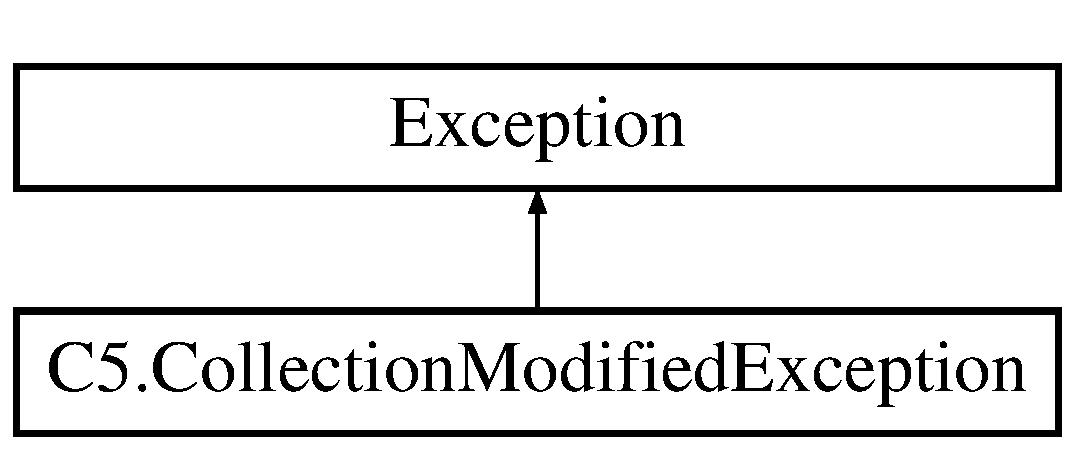
\includegraphics[height=2.000000cm]{class_c5_1_1_collection_modified_exception}
\end{center}
\end{figure}
\subsection*{Public Member Functions}
\begin{DoxyCompactItemize}
\item 
\hyperlink{class_c5_1_1_collection_modified_exception_af10bb3eee60db192722fb3e16c14cbc9}{Collection\+Modified\+Exception} ()
\begin{DoxyCompactList}\small\item\em Create a simple exception with no further explanation. \end{DoxyCompactList}\item 
\hyperlink{class_c5_1_1_collection_modified_exception_a891554e7e432faf411600c04f3143fe3}{Collection\+Modified\+Exception} (string message)
\begin{DoxyCompactList}\small\item\em Create the exception with an explanation of the reason. \end{DoxyCompactList}\end{DoxyCompactItemize}


\subsection{Detailed Description}
An exception thrown by enumerators, range views etc. when accessed after the underlying collection has been modified. 



\subsection{Constructor \& Destructor Documentation}
\hypertarget{class_c5_1_1_collection_modified_exception_af10bb3eee60db192722fb3e16c14cbc9}{}\index{C5\+::\+Collection\+Modified\+Exception@{C5\+::\+Collection\+Modified\+Exception}!Collection\+Modified\+Exception@{Collection\+Modified\+Exception}}
\index{Collection\+Modified\+Exception@{Collection\+Modified\+Exception}!C5\+::\+Collection\+Modified\+Exception@{C5\+::\+Collection\+Modified\+Exception}}
\subsubsection[{Collection\+Modified\+Exception()}]{\setlength{\rightskip}{0pt plus 5cm}C5.\+Collection\+Modified\+Exception.\+Collection\+Modified\+Exception (
\begin{DoxyParamCaption}
{}
\end{DoxyParamCaption}
)}\label{class_c5_1_1_collection_modified_exception_af10bb3eee60db192722fb3e16c14cbc9}


Create a simple exception with no further explanation. 

\hypertarget{class_c5_1_1_collection_modified_exception_a891554e7e432faf411600c04f3143fe3}{}\index{C5\+::\+Collection\+Modified\+Exception@{C5\+::\+Collection\+Modified\+Exception}!Collection\+Modified\+Exception@{Collection\+Modified\+Exception}}
\index{Collection\+Modified\+Exception@{Collection\+Modified\+Exception}!C5\+::\+Collection\+Modified\+Exception@{C5\+::\+Collection\+Modified\+Exception}}
\subsubsection[{Collection\+Modified\+Exception(string message)}]{\setlength{\rightskip}{0pt plus 5cm}C5.\+Collection\+Modified\+Exception.\+Collection\+Modified\+Exception (
\begin{DoxyParamCaption}
\item[{string}]{message}
\end{DoxyParamCaption}
)}\label{class_c5_1_1_collection_modified_exception_a891554e7e432faf411600c04f3143fe3}


Create the exception with an explanation of the reason. 


\begin{DoxyParams}{Parameters}
{\em message} & \\
\hline
\end{DoxyParams}


The documentation for this class was generated from the following file\+:\begin{DoxyCompactItemize}
\item 
C\+:/\+Users/rasmusl/\+Source/\+Repos/\+C5/\+C5/\hyperlink{_exceptions_8cs}{Exceptions.\+cs}\end{DoxyCompactItemize}

\hypertarget{class_c5_1_1_collection_value_base}{}\section{C5.\+Collection\+Value\+Base$<$ T $>$ Class Template Reference}
\label{class_c5_1_1_collection_value_base}\index{C5.\+Collection\+Value\+Base$<$ T $>$@{C5.\+Collection\+Value\+Base$<$ T $>$}}


Base class for classes implementing \hyperlink{interface_c5_1_1_i_collection_value}{I\+Collection\+Value}\mbox{[}T\mbox{]}  


Inheritance diagram for C5.\+Collection\+Value\+Base$<$ T $>$\+:\begin{figure}[H]
\begin{center}
\leavevmode
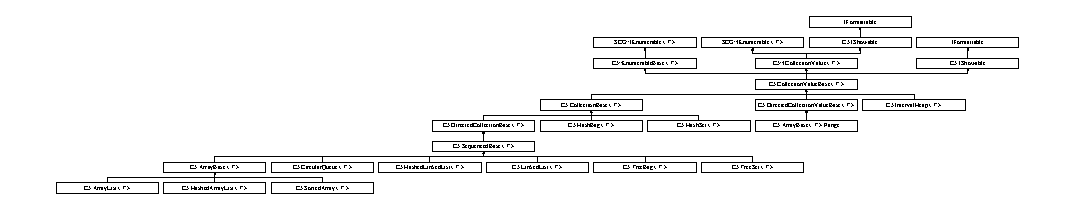
\includegraphics[height=2.372881cm]{class_c5_1_1_collection_value_base}
\end{center}
\end{figure}
\subsection*{Classes}
\begin{DoxyCompactItemize}
\item 
class \hyperlink{class_c5_1_1_collection_value_base_1_1_raise_for_remove_all_handler}{Raise\+For\+Remove\+All\+Handler}
\end{DoxyCompactItemize}
\subsection*{Public Member Functions}
\begin{DoxyCompactItemize}
\item 
virtual void \hyperlink{class_c5_1_1_collection_value_base_ab238770f168304e89664f814925522da}{Copy\+To} (T\mbox{[}$\,$\mbox{]} array, int index)
\begin{DoxyCompactList}\small\item\em Copy the items of this collection to part of an array. \end{DoxyCompactList}\item 
virtual T\mbox{[}$\,$\mbox{]} \hyperlink{class_c5_1_1_collection_value_base_a740757aebaa1365811e76729e59f338d}{To\+Array} ()
\begin{DoxyCompactList}\small\item\em Create an array with the items of this collection (in the same order as an enumerator would output them). \end{DoxyCompactList}\item 
virtual void \hyperlink{class_c5_1_1_collection_value_base_a1de9661198b86224773dcdc9d1678020}{Apply} (Action$<$ T $>$ action)
\begin{DoxyCompactList}\small\item\em Apply an single argument action, T\+:\+Action`1 to this enumerable \end{DoxyCompactList}\item 
virtual bool \hyperlink{class_c5_1_1_collection_value_base_af8e9e1630489ab12d89363cf4ab0e2ab}{Exists} (Func$<$ T, bool $>$ predicate)
\begin{DoxyCompactList}\small\item\em Check if there exists an item that satisfies a specific predicate in this collection. \end{DoxyCompactList}\item 
virtual bool \hyperlink{class_c5_1_1_collection_value_base_a90b979207d15086a9b64c9c689e17d4f}{Find} (Func$<$ T, bool $>$ predicate, out T item)
\begin{DoxyCompactList}\small\item\em Check if there exists an item that satisfies a specific predicate in this collection and return the first one in enumeration order. \end{DoxyCompactList}\item 
virtual bool \hyperlink{class_c5_1_1_collection_value_base_ad13a5bb7f735bf175add1e275b6d64ab}{All} (Func$<$ T, bool $>$ predicate)
\begin{DoxyCompactList}\small\item\em Check if all items in this collection satisfies a specific predicate. \end{DoxyCompactList}\item 
virtual S\+C\+G.\+I\+Enumerable$<$ T $>$ \hyperlink{class_c5_1_1_collection_value_base_a1e67c05020e8bebf39e0ddc9f55e5f32}{Filter} (Func$<$ T, bool $>$ predicate)
\begin{DoxyCompactList}\small\item\em Create an enumerable, enumerating the items of this collection that satisfies a certain condition. \end{DoxyCompactList}\item 
abstract T \hyperlink{class_c5_1_1_collection_value_base_ad7b8bd01dfd7ea8480a972f02a81608b}{Choose} ()
\begin{DoxyCompactList}\small\item\em Choose some item of this collection. \end{DoxyCompactList}\item 
abstract override S\+C\+G.\+I\+Enumerator$<$ T $>$ \hyperlink{class_c5_1_1_collection_value_base_a0e8b891322ed9987a18f1a1ac87d2d4f}{Get\+Enumerator} ()
\begin{DoxyCompactList}\small\item\em Create an enumerator for this collection. \end{DoxyCompactList}\item 
virtual bool \hyperlink{class_c5_1_1_collection_value_base_a96bd5814c13153aefae15ba969311c24}{Show} (System.\+Text.\+String\+Builder stringbuilder, ref int rest, I\+Format\+Provider format\+Provider)
\item 
virtual string \hyperlink{class_c5_1_1_collection_value_base_ad27cc9a47ff634613af0b5f0929de046}{To\+String} (string format, I\+Format\+Provider format\+Provider)
\item 
override string \hyperlink{class_c5_1_1_collection_value_base_a1fd928b586eb8af9378542d77e4de365}{To\+String} ()
\end{DoxyCompactItemize}
\subsection*{Protected Member Functions}
\begin{DoxyCompactItemize}
\item 
virtual void \hyperlink{class_c5_1_1_collection_value_base_a2479d8737c18958f6c725a0e38397825}{raise\+Collection\+Changed} ()
\begin{DoxyCompactList}\small\item\em Fire the Collection\+Changed event \end{DoxyCompactList}\item 
virtual void \hyperlink{class_c5_1_1_collection_value_base_a923cee6b9d57bf1694a070b21613f030}{raise\+Collection\+Cleared} (bool full, int count)
\begin{DoxyCompactList}\small\item\em Fire the Collection\+Cleared event \end{DoxyCompactList}\item 
virtual void \hyperlink{class_c5_1_1_collection_value_base_abcddaf7f4d7f64d41854e01dffd828ce}{raise\+Collection\+Cleared} (bool full, int count, int?offset)
\begin{DoxyCompactList}\small\item\em Fire the Collection\+Cleared event \end{DoxyCompactList}\item 
virtual void \hyperlink{class_c5_1_1_collection_value_base_a5c092cb991bc12200e7b893391fd8c38}{raise\+Items\+Added} (T item, int count)
\begin{DoxyCompactList}\small\item\em Fire the Items\+Added event \end{DoxyCompactList}\item 
virtual void \hyperlink{class_c5_1_1_collection_value_base_ade345c3e3c0d38d9694b569831a09752}{raise\+Items\+Removed} (T item, int count)
\begin{DoxyCompactList}\small\item\em Fire the Items\+Removed event \end{DoxyCompactList}\item 
virtual void \hyperlink{class_c5_1_1_collection_value_base_a053613a6d6d27e8cd2ad176b50b21b83}{raise\+Item\+Inserted} (T item, int index)
\begin{DoxyCompactList}\small\item\em Fire the Item\+Inserted event \end{DoxyCompactList}\item 
virtual void \hyperlink{class_c5_1_1_collection_value_base_a510a21c57e543cadb4ce4748b9099679}{raise\+Item\+Removed\+At} (T item, int index)
\begin{DoxyCompactList}\small\item\em Fire the Item\+Removed\+At event \end{DoxyCompactList}\item 
virtual void \hyperlink{class_c5_1_1_collection_value_base_a14876a0f26a0741ff82f3d851caa4602}{raise\+For\+Set\+This} (int index, T value, T item)
\item 
virtual void \hyperlink{class_c5_1_1_collection_value_base_a1f7ef395f3ad8027a2b32916a181b418}{raise\+For\+Insert} (int i, T item)
\item 
void \hyperlink{class_c5_1_1_collection_value_base_a2e014b2904d9ef88d3e15f6b0997f71b}{raise\+For\+Remove} (T item)
\item 
void \hyperlink{class_c5_1_1_collection_value_base_a95fcc3b52892d362b6118f57a8906cb8}{raise\+For\+Remove} (T item, int count)
\item 
void \hyperlink{class_c5_1_1_collection_value_base_ae15fee0551df68fa0e163604f920d601}{raise\+For\+Remove\+At} (int index, T item)
\item 
virtual void \hyperlink{class_c5_1_1_collection_value_base_ad76dc5138c43e80dd057007d78bb374d}{raise\+For\+Update} (T newitem, T olditem)
\item 
virtual void \hyperlink{class_c5_1_1_collection_value_base_ad05d49b820265d7e4e73c4f5992596b9}{raise\+For\+Update} (T newitem, T olditem, int count)
\item 
virtual void \hyperlink{class_c5_1_1_collection_value_base_a1048affd98d865d07454bcea754ec049}{raise\+For\+Add} (T item)
\item 
virtual void \hyperlink{class_c5_1_1_collection_value_base_a527018f12c5e83a0c99ea8c3ec4ac6ca}{raise\+For\+Remove\+All} (\hyperlink{interface_c5_1_1_i_collection_value}{I\+Collection\+Value}$<$ T $>$ was\+Removed)
\end{DoxyCompactItemize}
\subsection*{Properties}
\begin{DoxyCompactItemize}
\item 
virtual \hyperlink{namespace_c5_a9143bfd561fffa025d21561674758008}{Event\+Type\+Enum} \hyperlink{class_c5_1_1_collection_value_base_a5e6697e40d1421280e34fe47ebbdcefc}{Listenable\+Events}\hspace{0.3cm}{\ttfamily  \mbox{[}get\mbox{]}}
\item 
virtual \hyperlink{namespace_c5_a9143bfd561fffa025d21561674758008}{Event\+Type\+Enum} \hyperlink{class_c5_1_1_collection_value_base_a31ad6e1192e929ecd73a5f4e7e9332ba}{Active\+Events}\hspace{0.3cm}{\ttfamily  \mbox{[}get\mbox{]}}
\begin{DoxyCompactList}\small\item\em A flag bitmap of the events currently subscribed to by this collection. \end{DoxyCompactList}\item 
virtual Collection\+Changed\+Handler$<$ T $>$ \hyperlink{class_c5_1_1_collection_value_base_aba529af0877c1621812c2cc20e6dc7d9}{Collection\+Changed}
\begin{DoxyCompactList}\small\item\em The change event. Will be raised for every change operation on the collection. \end{DoxyCompactList}\item 
virtual Collection\+Cleared\+Handler$<$ T $>$ \hyperlink{class_c5_1_1_collection_value_base_ac3a3ee8103dbad9a0e647ef1a94bcf1f}{Collection\+Cleared}
\begin{DoxyCompactList}\small\item\em The clear event. Will be raised for every Clear operation on the collection. \end{DoxyCompactList}\item 
virtual Items\+Added\+Handler$<$ T $>$ \hyperlink{class_c5_1_1_collection_value_base_a3d7c78ee19bebf048061156c67aca5ef}{Items\+Added}
\begin{DoxyCompactList}\small\item\em The item added event. Will be raised for every individual addition to the collection. \end{DoxyCompactList}\item 
virtual Items\+Removed\+Handler$<$ T $>$ \hyperlink{class_c5_1_1_collection_value_base_a85608b4643299c9d576f68cf7cea70eb}{Items\+Removed}
\begin{DoxyCompactList}\small\item\em The item removed event. Will be raised for every individual removal from the collection. \end{DoxyCompactList}\item 
virtual Item\+Inserted\+Handler$<$ T $>$ \hyperlink{class_c5_1_1_collection_value_base_acfa66e3ccad2023f13ce71b2114e7809}{Item\+Inserted}
\begin{DoxyCompactList}\small\item\em The item added event. Will be raised for every individual addition to the collection. \end{DoxyCompactList}\item 
virtual Item\+Removed\+At\+Handler$<$ T $>$ \hyperlink{class_c5_1_1_collection_value_base_a9cd4d9d9e588e1a8fe51390906b3c66a}{Item\+Removed\+At}
\begin{DoxyCompactList}\small\item\em The item removed event. Will be raised for every individual removal from the collection. \end{DoxyCompactList}\item 
abstract bool \hyperlink{class_c5_1_1_collection_value_base_a9b906017c85e357268f116b3ac05e665}{Is\+Empty}\hspace{0.3cm}{\ttfamily  \mbox{[}get\mbox{]}}
\begin{DoxyCompactList}\small\item\em Check if collection is empty. \end{DoxyCompactList}\item 
abstract int \hyperlink{class_c5_1_1_collection_value_base_ac27de36f8fcd6bd3c66ce04768adfe1e}{Count}\hspace{0.3cm}{\ttfamily  \mbox{[}get\mbox{]}}
\begin{DoxyCompactList}\small\item\em The number of items in this collection. \end{DoxyCompactList}\item 
abstract \hyperlink{namespace_c5_a615ba88dcdaa8d5a3c5f833a73d7fad6}{Speed} \hyperlink{class_c5_1_1_collection_value_base_a29cca9929ed4b155a56f6c7297208ef3}{Count\+Speed}\hspace{0.3cm}{\ttfamily  \mbox{[}get\mbox{]}}
\begin{DoxyCompactList}\small\item\em The value is symbolic indicating the type of asymptotic complexity in terms of the size of this collection (worst-\/case or amortized as relevant). \end{DoxyCompactList}\end{DoxyCompactItemize}
\subsection*{Additional Inherited Members}


\subsection{Detailed Description}
Base class for classes implementing \hyperlink{interface_c5_1_1_i_collection_value}{I\+Collection\+Value}\mbox{[}T\mbox{]} 



\subsection{Member Function Documentation}
\hypertarget{class_c5_1_1_collection_value_base_ad13a5bb7f735bf175add1e275b6d64ab}{}\index{C5\+::\+Collection\+Value\+Base@{C5\+::\+Collection\+Value\+Base}!All@{All}}
\index{All@{All}!C5\+::\+Collection\+Value\+Base@{C5\+::\+Collection\+Value\+Base}}
\subsubsection[{All(\+Func$<$ T, bool $>$ predicate)}]{\setlength{\rightskip}{0pt plus 5cm}virtual bool {\bf C5.\+Collection\+Value\+Base}$<$ T $>$.All (
\begin{DoxyParamCaption}
\item[{Func$<$ T, bool $>$}]{predicate}
\end{DoxyParamCaption}
)\hspace{0.3cm}{\ttfamily [virtual]}}\label{class_c5_1_1_collection_value_base_ad13a5bb7f735bf175add1e275b6d64ab}


Check if all items in this collection satisfies a specific predicate. 


\begin{DoxyParams}{Parameters}
{\em predicate} & A delegate (T\+:\+Func`2 with 
\begin{DoxyCode}
R = \textcolor{keywordtype}{bool}
\end{DoxyCode}
) defining the predicate\\
\hline
\end{DoxyParams}
\begin{DoxyReturn}{Returns}
True if all items satisfies the predicate
\end{DoxyReturn}


Implements \hyperlink{interface_c5_1_1_i_collection_value_a099c3a257e5c0b7212e34e52a4a4bda2}{C5.\+I\+Collection\+Value$<$ T $>$}.

\hypertarget{class_c5_1_1_collection_value_base_a1de9661198b86224773dcdc9d1678020}{}\index{C5\+::\+Collection\+Value\+Base@{C5\+::\+Collection\+Value\+Base}!Apply@{Apply}}
\index{Apply@{Apply}!C5\+::\+Collection\+Value\+Base@{C5\+::\+Collection\+Value\+Base}}
\subsubsection[{Apply(\+Action$<$ T $>$ action)}]{\setlength{\rightskip}{0pt plus 5cm}virtual void {\bf C5.\+Collection\+Value\+Base}$<$ T $>$.Apply (
\begin{DoxyParamCaption}
\item[{Action$<$ T $>$}]{action}
\end{DoxyParamCaption}
)\hspace{0.3cm}{\ttfamily [virtual]}}\label{class_c5_1_1_collection_value_base_a1de9661198b86224773dcdc9d1678020}


Apply an single argument action, T\+:\+Action`1 to this enumerable 


\begin{DoxyParams}{Parameters}
{\em action} & The action delegate\\
\hline
\end{DoxyParams}


Implements \hyperlink{interface_c5_1_1_i_collection_value_aadcb9ce9d9362c0ade0c7d620e3cc182}{C5.\+I\+Collection\+Value$<$ T $>$}.

\hypertarget{class_c5_1_1_collection_value_base_ad7b8bd01dfd7ea8480a972f02a81608b}{}\index{C5\+::\+Collection\+Value\+Base@{C5\+::\+Collection\+Value\+Base}!Choose@{Choose}}
\index{Choose@{Choose}!C5\+::\+Collection\+Value\+Base@{C5\+::\+Collection\+Value\+Base}}
\subsubsection[{Choose()}]{\setlength{\rightskip}{0pt plus 5cm}abstract T {\bf C5.\+Collection\+Value\+Base}$<$ T $>$.Choose (
\begin{DoxyParamCaption}
{}
\end{DoxyParamCaption}
)\hspace{0.3cm}{\ttfamily [pure virtual]}}\label{class_c5_1_1_collection_value_base_ad7b8bd01dfd7ea8480a972f02a81608b}


Choose some item of this collection. 


\begin{DoxyExceptions}{Exceptions}
{\em \hyperlink{class_c5_1_1_no_such_item_exception}{No\+Such\+Item\+Exception}} & if collection is empty.\\
\hline
\end{DoxyExceptions}
\begin{DoxyReturn}{Returns}

\end{DoxyReturn}


Implements \hyperlink{interface_c5_1_1_i_collection_value_af72d52ddd8ea4130d508e1cf020cf7eb}{C5.\+I\+Collection\+Value$<$ T $>$}.



Implemented in \hyperlink{class_c5_1_1_hashed_linked_list_a8f4365d623d3424943b1891e998fc90d}{C5.\+Hashed\+Linked\+List$<$ T $>$}, \hyperlink{class_c5_1_1_linked_list_a50a8bc512629f661b2e98a1dc860cc9f}{C5.\+Linked\+List$<$ T $>$}, \hyperlink{class_c5_1_1_array_base_1_1_range_a914b2f3399f5286d462af7f1837373db}{C5.\+Array\+Base$<$ T $>$.\+Range}, \hyperlink{class_c5_1_1_array_base_a1d5f2551ce0fb795a5f2105fcb958de8}{C5.\+Array\+Base$<$ T $>$}, \hyperlink{class_c5_1_1_hash_set_a6bac17b51f5b2a569a0df8e0c46fe78f}{C5.\+Hash\+Set$<$ T $>$}, \hyperlink{class_c5_1_1_hash_bag_ac17786a0542bbe968fc662d5e2749265}{C5.\+Hash\+Bag$<$ T $>$}, \hyperlink{class_c5_1_1_tree_bag_a7b05001428a9e4605f556683a9bea20a}{C5.\+Tree\+Bag$<$ T $>$}, \hyperlink{class_c5_1_1_tree_set_aa4dd484b7c4363226e1053c8b2edd851}{C5.\+Tree\+Set$<$ T $>$}, \hyperlink{class_c5_1_1_interval_heap_a0d5fe1b0687d6ef002a17c6e46900772}{C5.\+Interval\+Heap$<$ T $>$}, \hyperlink{class_c5_1_1_circular_queue_aeabd2341783df834015d58b04c0c0a11}{C5.\+Circular\+Queue$<$ T $>$}, and \hyperlink{class_c5_1_1_mapped_collection_value_a355a9906ff7acccd3c2bd40ca11e5d1f}{C5.\+Mapped\+Collection\+Value$<$ T, V $>$}.

\hypertarget{class_c5_1_1_collection_value_base_ab238770f168304e89664f814925522da}{}\index{C5\+::\+Collection\+Value\+Base@{C5\+::\+Collection\+Value\+Base}!Copy\+To@{Copy\+To}}
\index{Copy\+To@{Copy\+To}!C5\+::\+Collection\+Value\+Base@{C5\+::\+Collection\+Value\+Base}}
\subsubsection[{Copy\+To(\+T[] array, int index)}]{\setlength{\rightskip}{0pt plus 5cm}virtual void {\bf C5.\+Collection\+Value\+Base}$<$ T $>$.Copy\+To (
\begin{DoxyParamCaption}
\item[{T\mbox{[}$\,$\mbox{]}}]{array, }
\item[{int}]{index}
\end{DoxyParamCaption}
)\hspace{0.3cm}{\ttfamily [virtual]}}\label{class_c5_1_1_collection_value_base_ab238770f168304e89664f814925522da}


Copy the items of this collection to part of an array. 


\begin{DoxyExceptions}{Exceptions}
{\em Argument\+Out\+Of\+Range\+Exception} & if 
\begin{DoxyCode}
index
\end{DoxyCode}
 is not a valid index into the array (i.\+e. negative or greater than the size of the array) or the array does not have room for the items.\\
\hline
\end{DoxyExceptions}

\begin{DoxyParams}{Parameters}
{\em array} & The array to copy to.\\
\hline
{\em index} & The starting index.\\
\hline
\end{DoxyParams}


Implements \hyperlink{interface_c5_1_1_i_collection_value_aced299d8dce69c33ff75b598e39581d1}{C5.\+I\+Collection\+Value$<$ T $>$}.



Reimplemented in \hyperlink{class_c5_1_1_hash_bag_ad7ffdb5c882c290aa8b398d499a9d2ac}{C5.\+Hash\+Bag$<$ T $>$}.

\hypertarget{class_c5_1_1_collection_value_base_af8e9e1630489ab12d89363cf4ab0e2ab}{}\index{C5\+::\+Collection\+Value\+Base@{C5\+::\+Collection\+Value\+Base}!Exists@{Exists}}
\index{Exists@{Exists}!C5\+::\+Collection\+Value\+Base@{C5\+::\+Collection\+Value\+Base}}
\subsubsection[{Exists(\+Func$<$ T, bool $>$ predicate)}]{\setlength{\rightskip}{0pt plus 5cm}virtual bool {\bf C5.\+Collection\+Value\+Base}$<$ T $>$.Exists (
\begin{DoxyParamCaption}
\item[{Func$<$ T, bool $>$}]{predicate}
\end{DoxyParamCaption}
)\hspace{0.3cm}{\ttfamily [virtual]}}\label{class_c5_1_1_collection_value_base_af8e9e1630489ab12d89363cf4ab0e2ab}


Check if there exists an item that satisfies a specific predicate in this collection. 


\begin{DoxyParams}{Parameters}
{\em predicate} & A delegate (T\+:\+Func`2 with 
\begin{DoxyCode}
R = \textcolor{keywordtype}{bool}
\end{DoxyCode}
) defining the predicate\\
\hline
\end{DoxyParams}
\begin{DoxyReturn}{Returns}
True if such an item exists
\end{DoxyReturn}


Implements \hyperlink{interface_c5_1_1_i_collection_value_a3c20f35782dbd046f9aba5ec13dad789}{C5.\+I\+Collection\+Value$<$ T $>$}.

\hypertarget{class_c5_1_1_collection_value_base_a1e67c05020e8bebf39e0ddc9f55e5f32}{}\index{C5\+::\+Collection\+Value\+Base@{C5\+::\+Collection\+Value\+Base}!Filter@{Filter}}
\index{Filter@{Filter}!C5\+::\+Collection\+Value\+Base@{C5\+::\+Collection\+Value\+Base}}
\subsubsection[{Filter(\+Func$<$ T, bool $>$ predicate)}]{\setlength{\rightskip}{0pt plus 5cm}virtual S\+C\+G.\+I\+Enumerable$<$T$>$ {\bf C5.\+Collection\+Value\+Base}$<$ T $>$.Filter (
\begin{DoxyParamCaption}
\item[{Func$<$ T, bool $>$}]{predicate}
\end{DoxyParamCaption}
)\hspace{0.3cm}{\ttfamily [virtual]}}\label{class_c5_1_1_collection_value_base_a1e67c05020e8bebf39e0ddc9f55e5f32}


Create an enumerable, enumerating the items of this collection that satisfies a certain condition. 


\begin{DoxyParams}{Parameters}
{\em predicate} & A delegate (T\+:\+Func`2 with 
\begin{DoxyCode}
R = \textcolor{keywordtype}{bool}
\end{DoxyCode}
) defining the predicate\\
\hline
\end{DoxyParams}
\begin{DoxyReturn}{Returns}
The filtered enumerable
\end{DoxyReturn}


Implements \hyperlink{interface_c5_1_1_i_collection_value_a485e8b464ed5dfb5f2ff5dc10a8a62d6}{C5.\+I\+Collection\+Value$<$ T $>$}.



Reimplemented in \hyperlink{class_c5_1_1_hashed_linked_list_ad092b0255821d358df6cfe045870e256}{C5.\+Hashed\+Linked\+List$<$ T $>$}, and \hyperlink{class_c5_1_1_linked_list_a5027335e5234dc6a6e3a164d79ccae62}{C5.\+Linked\+List$<$ T $>$}.

\hypertarget{class_c5_1_1_collection_value_base_a90b979207d15086a9b64c9c689e17d4f}{}\index{C5\+::\+Collection\+Value\+Base@{C5\+::\+Collection\+Value\+Base}!Find@{Find}}
\index{Find@{Find}!C5\+::\+Collection\+Value\+Base@{C5\+::\+Collection\+Value\+Base}}
\subsubsection[{Find(\+Func$<$ T, bool $>$ predicate, out T item)}]{\setlength{\rightskip}{0pt plus 5cm}virtual bool {\bf C5.\+Collection\+Value\+Base}$<$ T $>$.Find (
\begin{DoxyParamCaption}
\item[{Func$<$ T, bool $>$}]{predicate, }
\item[{out T}]{item}
\end{DoxyParamCaption}
)\hspace{0.3cm}{\ttfamily [virtual]}}\label{class_c5_1_1_collection_value_base_a90b979207d15086a9b64c9c689e17d4f}


Check if there exists an item that satisfies a specific predicate in this collection and return the first one in enumeration order. 


\begin{DoxyParams}{Parameters}
{\em predicate} & A delegate (T\+:\+Func`2 with 
\begin{DoxyCode}
R == \textcolor{keywordtype}{bool}
\end{DoxyCode}
) defining the predicate\\
\hline
{\em item} & \\
\hline
\end{DoxyParams}
\begin{DoxyReturn}{Returns}
True is such an item exists
\end{DoxyReturn}


Implements \hyperlink{interface_c5_1_1_i_collection_value_a3e175f833398fa6a6cde45e4948bc152}{C5.\+I\+Collection\+Value$<$ T $>$}.

\hypertarget{class_c5_1_1_collection_value_base_a0e8b891322ed9987a18f1a1ac87d2d4f}{}\index{C5\+::\+Collection\+Value\+Base@{C5\+::\+Collection\+Value\+Base}!Get\+Enumerator@{Get\+Enumerator}}
\index{Get\+Enumerator@{Get\+Enumerator}!C5\+::\+Collection\+Value\+Base@{C5\+::\+Collection\+Value\+Base}}
\subsubsection[{Get\+Enumerator()}]{\setlength{\rightskip}{0pt plus 5cm}abstract override S\+C\+G.\+I\+Enumerator$<$T$>$ {\bf C5.\+Collection\+Value\+Base}$<$ T $>$.Get\+Enumerator (
\begin{DoxyParamCaption}
{}
\end{DoxyParamCaption}
)\hspace{0.3cm}{\ttfamily [pure virtual]}}\label{class_c5_1_1_collection_value_base_a0e8b891322ed9987a18f1a1ac87d2d4f}


Create an enumerator for this collection. 

\begin{DoxyReturn}{Returns}
The enumerator
\end{DoxyReturn}


Implements \hyperlink{class_c5_1_1_enumerable_base_ad8893620ea9cc4e7d41c17d26769d237}{C5.\+Enumerable\+Base$<$ T $>$}.



Implemented in \hyperlink{class_c5_1_1_hashed_linked_list_ae8f40668f13afb6cb05501446a3bcc4e}{C5.\+Hashed\+Linked\+List$<$ T $>$}, \hyperlink{class_c5_1_1_linked_list_ab23965434fba5e39a15eb4c0eb3c4901}{C5.\+Linked\+List$<$ T $>$}, \hyperlink{class_c5_1_1_hashed_array_list_a0ce81bee1c45ccbc3105698a4f4692a8}{C5.\+Hashed\+Array\+List$<$ T $>$}, \hyperlink{class_c5_1_1_array_list_ae6c2dc2f2aa8c9952d3267a37e9de01a}{C5.\+Array\+List$<$ T $>$}, \hyperlink{class_c5_1_1_array_base_1_1_range_af6396c46d77d98185e8587c024dd9316}{C5.\+Array\+Base$<$ T $>$.\+Range}, \hyperlink{class_c5_1_1_array_base_a84a54c5fa039db32e27ca45c6b0cea85}{C5.\+Array\+Base$<$ T $>$}, \hyperlink{class_c5_1_1_sequenced_base_a07d117175b630fd7f87f6e61b05259dc}{C5.\+Sequenced\+Base$<$ T $>$}, \hyperlink{class_c5_1_1_collection_base_a3b4b98e2606afecb948019412c4c2533}{C5.\+Collection\+Base$<$ T $>$}, \hyperlink{class_c5_1_1_hash_set_a4c404a22695abc0f6b47bf74d3d34034}{C5.\+Hash\+Set$<$ T $>$}, \hyperlink{class_c5_1_1_hash_bag_a621d77b2f8a7c3a826aace4be1d809b2}{C5.\+Hash\+Bag$<$ T $>$}, \hyperlink{class_c5_1_1_tree_bag_a2c00797c0e29dd52efa05f219b4c9c7e}{C5.\+Tree\+Bag$<$ T $>$}, \hyperlink{class_c5_1_1_tree_set_af9dd4aece1415276e1ede1ded6904179}{C5.\+Tree\+Set$<$ T $>$}, \hyperlink{class_c5_1_1_interval_heap_a09556ba66252a46d94456587bc877561}{C5.\+Interval\+Heap$<$ T $>$}, \hyperlink{class_c5_1_1_circular_queue_ae1ab5e745ced280db9b9a175a66dc5b4}{C5.\+Circular\+Queue$<$ T $>$}, and \hyperlink{class_c5_1_1_mapped_collection_value_ab4c51f484c9d5569b7f8c9f1bf4ab231}{C5.\+Mapped\+Collection\+Value$<$ T, V $>$}.

\hypertarget{class_c5_1_1_collection_value_base_a2479d8737c18958f6c725a0e38397825}{}\index{C5\+::\+Collection\+Value\+Base@{C5\+::\+Collection\+Value\+Base}!raise\+Collection\+Changed@{raise\+Collection\+Changed}}
\index{raise\+Collection\+Changed@{raise\+Collection\+Changed}!C5\+::\+Collection\+Value\+Base@{C5\+::\+Collection\+Value\+Base}}
\subsubsection[{raise\+Collection\+Changed()}]{\setlength{\rightskip}{0pt plus 5cm}virtual void {\bf C5.\+Collection\+Value\+Base}$<$ T $>$.raise\+Collection\+Changed (
\begin{DoxyParamCaption}
{}
\end{DoxyParamCaption}
)\hspace{0.3cm}{\ttfamily [protected]}, {\ttfamily [virtual]}}\label{class_c5_1_1_collection_value_base_a2479d8737c18958f6c725a0e38397825}


Fire the Collection\+Changed event 

\hypertarget{class_c5_1_1_collection_value_base_a923cee6b9d57bf1694a070b21613f030}{}\index{C5\+::\+Collection\+Value\+Base@{C5\+::\+Collection\+Value\+Base}!raise\+Collection\+Cleared@{raise\+Collection\+Cleared}}
\index{raise\+Collection\+Cleared@{raise\+Collection\+Cleared}!C5\+::\+Collection\+Value\+Base@{C5\+::\+Collection\+Value\+Base}}
\subsubsection[{raise\+Collection\+Cleared(bool full, int count)}]{\setlength{\rightskip}{0pt plus 5cm}virtual void {\bf C5.\+Collection\+Value\+Base}$<$ T $>$.raise\+Collection\+Cleared (
\begin{DoxyParamCaption}
\item[{bool}]{full, }
\item[{int}]{count}
\end{DoxyParamCaption}
)\hspace{0.3cm}{\ttfamily [protected]}, {\ttfamily [virtual]}}\label{class_c5_1_1_collection_value_base_a923cee6b9d57bf1694a070b21613f030}


Fire the Collection\+Cleared event 

\hypertarget{class_c5_1_1_collection_value_base_abcddaf7f4d7f64d41854e01dffd828ce}{}\index{C5\+::\+Collection\+Value\+Base@{C5\+::\+Collection\+Value\+Base}!raise\+Collection\+Cleared@{raise\+Collection\+Cleared}}
\index{raise\+Collection\+Cleared@{raise\+Collection\+Cleared}!C5\+::\+Collection\+Value\+Base@{C5\+::\+Collection\+Value\+Base}}
\subsubsection[{raise\+Collection\+Cleared(bool full, int count, int?offset)}]{\setlength{\rightskip}{0pt plus 5cm}virtual void {\bf C5.\+Collection\+Value\+Base}$<$ T $>$.raise\+Collection\+Cleared (
\begin{DoxyParamCaption}
\item[{bool}]{full, }
\item[{int}]{count, }
\item[{int?}]{offset}
\end{DoxyParamCaption}
)\hspace{0.3cm}{\ttfamily [protected]}, {\ttfamily [virtual]}}\label{class_c5_1_1_collection_value_base_abcddaf7f4d7f64d41854e01dffd828ce}


Fire the Collection\+Cleared event 

\hypertarget{class_c5_1_1_collection_value_base_a1048affd98d865d07454bcea754ec049}{}\index{C5\+::\+Collection\+Value\+Base@{C5\+::\+Collection\+Value\+Base}!raise\+For\+Add@{raise\+For\+Add}}
\index{raise\+For\+Add@{raise\+For\+Add}!C5\+::\+Collection\+Value\+Base@{C5\+::\+Collection\+Value\+Base}}
\subsubsection[{raise\+For\+Add(\+T item)}]{\setlength{\rightskip}{0pt plus 5cm}virtual void {\bf C5.\+Collection\+Value\+Base}$<$ T $>$.raise\+For\+Add (
\begin{DoxyParamCaption}
\item[{T}]{item}
\end{DoxyParamCaption}
)\hspace{0.3cm}{\ttfamily [protected]}, {\ttfamily [virtual]}}\label{class_c5_1_1_collection_value_base_a1048affd98d865d07454bcea754ec049}





\begin{DoxyParams}{Parameters}
{\em item} & \\
\hline
\end{DoxyParams}
\hypertarget{class_c5_1_1_collection_value_base_a1f7ef395f3ad8027a2b32916a181b418}{}\index{C5\+::\+Collection\+Value\+Base@{C5\+::\+Collection\+Value\+Base}!raise\+For\+Insert@{raise\+For\+Insert}}
\index{raise\+For\+Insert@{raise\+For\+Insert}!C5\+::\+Collection\+Value\+Base@{C5\+::\+Collection\+Value\+Base}}
\subsubsection[{raise\+For\+Insert(int i, T item)}]{\setlength{\rightskip}{0pt plus 5cm}virtual void {\bf C5.\+Collection\+Value\+Base}$<$ T $>$.raise\+For\+Insert (
\begin{DoxyParamCaption}
\item[{int}]{i, }
\item[{T}]{item}
\end{DoxyParamCaption}
)\hspace{0.3cm}{\ttfamily [protected]}, {\ttfamily [virtual]}}\label{class_c5_1_1_collection_value_base_a1f7ef395f3ad8027a2b32916a181b418}





\begin{DoxyParams}{Parameters}
{\em i} & \\
\hline
{\em item} & \\
\hline
\end{DoxyParams}
\hypertarget{class_c5_1_1_collection_value_base_a2e014b2904d9ef88d3e15f6b0997f71b}{}\index{C5\+::\+Collection\+Value\+Base@{C5\+::\+Collection\+Value\+Base}!raise\+For\+Remove@{raise\+For\+Remove}}
\index{raise\+For\+Remove@{raise\+For\+Remove}!C5\+::\+Collection\+Value\+Base@{C5\+::\+Collection\+Value\+Base}}
\subsubsection[{raise\+For\+Remove(\+T item)}]{\setlength{\rightskip}{0pt plus 5cm}void {\bf C5.\+Collection\+Value\+Base}$<$ T $>$.raise\+For\+Remove (
\begin{DoxyParamCaption}
\item[{T}]{item}
\end{DoxyParamCaption}
)\hspace{0.3cm}{\ttfamily [protected]}}\label{class_c5_1_1_collection_value_base_a2e014b2904d9ef88d3e15f6b0997f71b}





\begin{DoxyParams}{Parameters}
{\em item} & \\
\hline
\end{DoxyParams}
\hypertarget{class_c5_1_1_collection_value_base_a95fcc3b52892d362b6118f57a8906cb8}{}\index{C5\+::\+Collection\+Value\+Base@{C5\+::\+Collection\+Value\+Base}!raise\+For\+Remove@{raise\+For\+Remove}}
\index{raise\+For\+Remove@{raise\+For\+Remove}!C5\+::\+Collection\+Value\+Base@{C5\+::\+Collection\+Value\+Base}}
\subsubsection[{raise\+For\+Remove(\+T item, int count)}]{\setlength{\rightskip}{0pt plus 5cm}void {\bf C5.\+Collection\+Value\+Base}$<$ T $>$.raise\+For\+Remove (
\begin{DoxyParamCaption}
\item[{T}]{item, }
\item[{int}]{count}
\end{DoxyParamCaption}
)\hspace{0.3cm}{\ttfamily [protected]}}\label{class_c5_1_1_collection_value_base_a95fcc3b52892d362b6118f57a8906cb8}





\begin{DoxyParams}{Parameters}
{\em item} & \\
\hline
{\em count} & \\
\hline
\end{DoxyParams}
\hypertarget{class_c5_1_1_collection_value_base_a527018f12c5e83a0c99ea8c3ec4ac6ca}{}\index{C5\+::\+Collection\+Value\+Base@{C5\+::\+Collection\+Value\+Base}!raise\+For\+Remove\+All@{raise\+For\+Remove\+All}}
\index{raise\+For\+Remove\+All@{raise\+For\+Remove\+All}!C5\+::\+Collection\+Value\+Base@{C5\+::\+Collection\+Value\+Base}}
\subsubsection[{raise\+For\+Remove\+All(\+I\+Collection\+Value$<$ T $>$ was\+Removed)}]{\setlength{\rightskip}{0pt plus 5cm}virtual void {\bf C5.\+Collection\+Value\+Base}$<$ T $>$.raise\+For\+Remove\+All (
\begin{DoxyParamCaption}
\item[{{\bf I\+Collection\+Value}$<$ T $>$}]{was\+Removed}
\end{DoxyParamCaption}
)\hspace{0.3cm}{\ttfamily [protected]}, {\ttfamily [virtual]}}\label{class_c5_1_1_collection_value_base_a527018f12c5e83a0c99ea8c3ec4ac6ca}





\begin{DoxyParams}{Parameters}
{\em was\+Removed} & \\
\hline
\end{DoxyParams}
\hypertarget{class_c5_1_1_collection_value_base_ae15fee0551df68fa0e163604f920d601}{}\index{C5\+::\+Collection\+Value\+Base@{C5\+::\+Collection\+Value\+Base}!raise\+For\+Remove\+At@{raise\+For\+Remove\+At}}
\index{raise\+For\+Remove\+At@{raise\+For\+Remove\+At}!C5\+::\+Collection\+Value\+Base@{C5\+::\+Collection\+Value\+Base}}
\subsubsection[{raise\+For\+Remove\+At(int index, T item)}]{\setlength{\rightskip}{0pt plus 5cm}void {\bf C5.\+Collection\+Value\+Base}$<$ T $>$.raise\+For\+Remove\+At (
\begin{DoxyParamCaption}
\item[{int}]{index, }
\item[{T}]{item}
\end{DoxyParamCaption}
)\hspace{0.3cm}{\ttfamily [protected]}}\label{class_c5_1_1_collection_value_base_ae15fee0551df68fa0e163604f920d601}





\begin{DoxyParams}{Parameters}
{\em index} & \\
\hline
{\em item} & \\
\hline
\end{DoxyParams}
\hypertarget{class_c5_1_1_collection_value_base_a14876a0f26a0741ff82f3d851caa4602}{}\index{C5\+::\+Collection\+Value\+Base@{C5\+::\+Collection\+Value\+Base}!raise\+For\+Set\+This@{raise\+For\+Set\+This}}
\index{raise\+For\+Set\+This@{raise\+For\+Set\+This}!C5\+::\+Collection\+Value\+Base@{C5\+::\+Collection\+Value\+Base}}
\subsubsection[{raise\+For\+Set\+This(int index, T value, T item)}]{\setlength{\rightskip}{0pt plus 5cm}virtual void {\bf C5.\+Collection\+Value\+Base}$<$ T $>$.raise\+For\+Set\+This (
\begin{DoxyParamCaption}
\item[{int}]{index, }
\item[{T}]{value, }
\item[{T}]{item}
\end{DoxyParamCaption}
)\hspace{0.3cm}{\ttfamily [protected]}, {\ttfamily [virtual]}}\label{class_c5_1_1_collection_value_base_a14876a0f26a0741ff82f3d851caa4602}





\begin{DoxyParams}{Parameters}
{\em index} & \\
\hline
{\em value} & \\
\hline
{\em item} & \\
\hline
\end{DoxyParams}
\hypertarget{class_c5_1_1_collection_value_base_ad76dc5138c43e80dd057007d78bb374d}{}\index{C5\+::\+Collection\+Value\+Base@{C5\+::\+Collection\+Value\+Base}!raise\+For\+Update@{raise\+For\+Update}}
\index{raise\+For\+Update@{raise\+For\+Update}!C5\+::\+Collection\+Value\+Base@{C5\+::\+Collection\+Value\+Base}}
\subsubsection[{raise\+For\+Update(\+T newitem, T olditem)}]{\setlength{\rightskip}{0pt plus 5cm}virtual void {\bf C5.\+Collection\+Value\+Base}$<$ T $>$.raise\+For\+Update (
\begin{DoxyParamCaption}
\item[{T}]{newitem, }
\item[{T}]{olditem}
\end{DoxyParamCaption}
)\hspace{0.3cm}{\ttfamily [protected]}, {\ttfamily [virtual]}}\label{class_c5_1_1_collection_value_base_ad76dc5138c43e80dd057007d78bb374d}





\begin{DoxyParams}{Parameters}
{\em newitem} & \\
\hline
{\em olditem} & \\
\hline
\end{DoxyParams}
\hypertarget{class_c5_1_1_collection_value_base_ad05d49b820265d7e4e73c4f5992596b9}{}\index{C5\+::\+Collection\+Value\+Base@{C5\+::\+Collection\+Value\+Base}!raise\+For\+Update@{raise\+For\+Update}}
\index{raise\+For\+Update@{raise\+For\+Update}!C5\+::\+Collection\+Value\+Base@{C5\+::\+Collection\+Value\+Base}}
\subsubsection[{raise\+For\+Update(\+T newitem, T olditem, int count)}]{\setlength{\rightskip}{0pt plus 5cm}virtual void {\bf C5.\+Collection\+Value\+Base}$<$ T $>$.raise\+For\+Update (
\begin{DoxyParamCaption}
\item[{T}]{newitem, }
\item[{T}]{olditem, }
\item[{int}]{count}
\end{DoxyParamCaption}
)\hspace{0.3cm}{\ttfamily [protected]}, {\ttfamily [virtual]}}\label{class_c5_1_1_collection_value_base_ad05d49b820265d7e4e73c4f5992596b9}





\begin{DoxyParams}{Parameters}
{\em newitem} & \\
\hline
{\em olditem} & \\
\hline
{\em count} & \\
\hline
\end{DoxyParams}
\hypertarget{class_c5_1_1_collection_value_base_a053613a6d6d27e8cd2ad176b50b21b83}{}\index{C5\+::\+Collection\+Value\+Base@{C5\+::\+Collection\+Value\+Base}!raise\+Item\+Inserted@{raise\+Item\+Inserted}}
\index{raise\+Item\+Inserted@{raise\+Item\+Inserted}!C5\+::\+Collection\+Value\+Base@{C5\+::\+Collection\+Value\+Base}}
\subsubsection[{raise\+Item\+Inserted(\+T item, int index)}]{\setlength{\rightskip}{0pt plus 5cm}virtual void {\bf C5.\+Collection\+Value\+Base}$<$ T $>$.raise\+Item\+Inserted (
\begin{DoxyParamCaption}
\item[{T}]{item, }
\item[{int}]{index}
\end{DoxyParamCaption}
)\hspace{0.3cm}{\ttfamily [protected]}, {\ttfamily [virtual]}}\label{class_c5_1_1_collection_value_base_a053613a6d6d27e8cd2ad176b50b21b83}


Fire the Item\+Inserted event 


\begin{DoxyParams}{Parameters}
{\em item} & The item that was added\\
\hline
{\em index} & \\
\hline
\end{DoxyParams}
\hypertarget{class_c5_1_1_collection_value_base_a510a21c57e543cadb4ce4748b9099679}{}\index{C5\+::\+Collection\+Value\+Base@{C5\+::\+Collection\+Value\+Base}!raise\+Item\+Removed\+At@{raise\+Item\+Removed\+At}}
\index{raise\+Item\+Removed\+At@{raise\+Item\+Removed\+At}!C5\+::\+Collection\+Value\+Base@{C5\+::\+Collection\+Value\+Base}}
\subsubsection[{raise\+Item\+Removed\+At(\+T item, int index)}]{\setlength{\rightskip}{0pt plus 5cm}virtual void {\bf C5.\+Collection\+Value\+Base}$<$ T $>$.raise\+Item\+Removed\+At (
\begin{DoxyParamCaption}
\item[{T}]{item, }
\item[{int}]{index}
\end{DoxyParamCaption}
)\hspace{0.3cm}{\ttfamily [protected]}, {\ttfamily [virtual]}}\label{class_c5_1_1_collection_value_base_a510a21c57e543cadb4ce4748b9099679}


Fire the Item\+Removed\+At event 


\begin{DoxyParams}{Parameters}
{\em item} & The item that was removed\\
\hline
{\em index} & \\
\hline
\end{DoxyParams}
\hypertarget{class_c5_1_1_collection_value_base_a5c092cb991bc12200e7b893391fd8c38}{}\index{C5\+::\+Collection\+Value\+Base@{C5\+::\+Collection\+Value\+Base}!raise\+Items\+Added@{raise\+Items\+Added}}
\index{raise\+Items\+Added@{raise\+Items\+Added}!C5\+::\+Collection\+Value\+Base@{C5\+::\+Collection\+Value\+Base}}
\subsubsection[{raise\+Items\+Added(\+T item, int count)}]{\setlength{\rightskip}{0pt plus 5cm}virtual void {\bf C5.\+Collection\+Value\+Base}$<$ T $>$.raise\+Items\+Added (
\begin{DoxyParamCaption}
\item[{T}]{item, }
\item[{int}]{count}
\end{DoxyParamCaption}
)\hspace{0.3cm}{\ttfamily [protected]}, {\ttfamily [virtual]}}\label{class_c5_1_1_collection_value_base_a5c092cb991bc12200e7b893391fd8c38}


Fire the Items\+Added event 


\begin{DoxyParams}{Parameters}
{\em item} & The item that was added\\
\hline
{\em count} & \\
\hline
\end{DoxyParams}
\hypertarget{class_c5_1_1_collection_value_base_ade345c3e3c0d38d9694b569831a09752}{}\index{C5\+::\+Collection\+Value\+Base@{C5\+::\+Collection\+Value\+Base}!raise\+Items\+Removed@{raise\+Items\+Removed}}
\index{raise\+Items\+Removed@{raise\+Items\+Removed}!C5\+::\+Collection\+Value\+Base@{C5\+::\+Collection\+Value\+Base}}
\subsubsection[{raise\+Items\+Removed(\+T item, int count)}]{\setlength{\rightskip}{0pt plus 5cm}virtual void {\bf C5.\+Collection\+Value\+Base}$<$ T $>$.raise\+Items\+Removed (
\begin{DoxyParamCaption}
\item[{T}]{item, }
\item[{int}]{count}
\end{DoxyParamCaption}
)\hspace{0.3cm}{\ttfamily [protected]}, {\ttfamily [virtual]}}\label{class_c5_1_1_collection_value_base_ade345c3e3c0d38d9694b569831a09752}


Fire the Items\+Removed event 


\begin{DoxyParams}{Parameters}
{\em item} & The item that was removed\\
\hline
{\em count} & \\
\hline
\end{DoxyParams}
\hypertarget{class_c5_1_1_collection_value_base_a96bd5814c13153aefae15ba969311c24}{}\index{C5\+::\+Collection\+Value\+Base@{C5\+::\+Collection\+Value\+Base}!Show@{Show}}
\index{Show@{Show}!C5\+::\+Collection\+Value\+Base@{C5\+::\+Collection\+Value\+Base}}
\subsubsection[{Show(\+System.\+Text.\+String\+Builder stringbuilder, ref int rest, I\+Format\+Provider format\+Provider)}]{\setlength{\rightskip}{0pt plus 5cm}virtual bool {\bf C5.\+Collection\+Value\+Base}$<$ T $>$.Show (
\begin{DoxyParamCaption}
\item[{System.\+Text.\+String\+Builder}]{stringbuilder, }
\item[{ref int}]{rest, }
\item[{I\+Format\+Provider}]{format\+Provider}
\end{DoxyParamCaption}
)\hspace{0.3cm}{\ttfamily [virtual]}}\label{class_c5_1_1_collection_value_base_a96bd5814c13153aefae15ba969311c24}





\begin{DoxyParams}{Parameters}
{\em stringbuilder} & \\
\hline
{\em rest} & \\
\hline
{\em format\+Provider} & \\
\hline
\end{DoxyParams}
\begin{DoxyReturn}{Returns}

\end{DoxyReturn}
\hypertarget{class_c5_1_1_collection_value_base_a740757aebaa1365811e76729e59f338d}{}\index{C5\+::\+Collection\+Value\+Base@{C5\+::\+Collection\+Value\+Base}!To\+Array@{To\+Array}}
\index{To\+Array@{To\+Array}!C5\+::\+Collection\+Value\+Base@{C5\+::\+Collection\+Value\+Base}}
\subsubsection[{To\+Array()}]{\setlength{\rightskip}{0pt plus 5cm}virtual T \mbox{[}$\,$\mbox{]} {\bf C5.\+Collection\+Value\+Base}$<$ T $>$.To\+Array (
\begin{DoxyParamCaption}
{}
\end{DoxyParamCaption}
)\hspace{0.3cm}{\ttfamily [virtual]}}\label{class_c5_1_1_collection_value_base_a740757aebaa1365811e76729e59f338d}


Create an array with the items of this collection (in the same order as an enumerator would output them). 

\begin{DoxyReturn}{Returns}
The array
\end{DoxyReturn}


Implements \hyperlink{interface_c5_1_1_i_collection_value_ad76547324e71a04e92076b2e55239bbb}{C5.\+I\+Collection\+Value$<$ T $>$}.



Reimplemented in \hyperlink{class_c5_1_1_array_base_a16ffcc583a32065194b3ea27d4a43cd4}{C5.\+Array\+Base$<$ T $>$}, \hyperlink{class_c5_1_1_hash_set_ad6e22ebc64d9f8c96b805547d5873023}{C5.\+Hash\+Set$<$ T $>$}, and \hyperlink{class_c5_1_1_hash_bag_a7be4bcb7a5ef7f9414a33cfb9439e15e}{C5.\+Hash\+Bag$<$ T $>$}.

\hypertarget{class_c5_1_1_collection_value_base_ad27cc9a47ff634613af0b5f0929de046}{}\index{C5\+::\+Collection\+Value\+Base@{C5\+::\+Collection\+Value\+Base}!To\+String@{To\+String}}
\index{To\+String@{To\+String}!C5\+::\+Collection\+Value\+Base@{C5\+::\+Collection\+Value\+Base}}
\subsubsection[{To\+String(string format, I\+Format\+Provider format\+Provider)}]{\setlength{\rightskip}{0pt plus 5cm}virtual string {\bf C5.\+Collection\+Value\+Base}$<$ T $>$.To\+String (
\begin{DoxyParamCaption}
\item[{string}]{format, }
\item[{I\+Format\+Provider}]{format\+Provider}
\end{DoxyParamCaption}
)\hspace{0.3cm}{\ttfamily [virtual]}}\label{class_c5_1_1_collection_value_base_ad27cc9a47ff634613af0b5f0929de046}





\begin{DoxyParams}{Parameters}
{\em format} & \\
\hline
{\em format\+Provider} & \\
\hline
\end{DoxyParams}
\begin{DoxyReturn}{Returns}

\end{DoxyReturn}
\hypertarget{class_c5_1_1_collection_value_base_a1fd928b586eb8af9378542d77e4de365}{}\index{C5\+::\+Collection\+Value\+Base@{C5\+::\+Collection\+Value\+Base}!To\+String@{To\+String}}
\index{To\+String@{To\+String}!C5\+::\+Collection\+Value\+Base@{C5\+::\+Collection\+Value\+Base}}
\subsubsection[{To\+String()}]{\setlength{\rightskip}{0pt plus 5cm}override string {\bf C5.\+Collection\+Value\+Base}$<$ T $>$.To\+String (
\begin{DoxyParamCaption}
{}
\end{DoxyParamCaption}
)}\label{class_c5_1_1_collection_value_base_a1fd928b586eb8af9378542d77e4de365}




\begin{DoxyReturn}{Returns}

\end{DoxyReturn}


\subsection{Property Documentation}
\hypertarget{class_c5_1_1_collection_value_base_a31ad6e1192e929ecd73a5f4e7e9332ba}{}\index{C5\+::\+Collection\+Value\+Base@{C5\+::\+Collection\+Value\+Base}!Active\+Events@{Active\+Events}}
\index{Active\+Events@{Active\+Events}!C5\+::\+Collection\+Value\+Base@{C5\+::\+Collection\+Value\+Base}}
\subsubsection[{Active\+Events}]{\setlength{\rightskip}{0pt plus 5cm}virtual {\bf Event\+Type\+Enum} {\bf C5.\+Collection\+Value\+Base}$<$ T $>$.Active\+Events\hspace{0.3cm}{\ttfamily [get]}}\label{class_c5_1_1_collection_value_base_a31ad6e1192e929ecd73a5f4e7e9332ba}


A flag bitmap of the events currently subscribed to by this collection. 

\hypertarget{class_c5_1_1_collection_value_base_aba529af0877c1621812c2cc20e6dc7d9}{}\index{C5\+::\+Collection\+Value\+Base@{C5\+::\+Collection\+Value\+Base}!Collection\+Changed@{Collection\+Changed}}
\index{Collection\+Changed@{Collection\+Changed}!C5\+::\+Collection\+Value\+Base@{C5\+::\+Collection\+Value\+Base}}
\subsubsection[{Collection\+Changed}]{\setlength{\rightskip}{0pt plus 5cm}virtual Collection\+Changed\+Handler$<$T$>$ {\bf C5.\+Collection\+Value\+Base}$<$ T $>$.Collection\+Changed\hspace{0.3cm}{\ttfamily [add]}, {\ttfamily [remove]}}\label{class_c5_1_1_collection_value_base_aba529af0877c1621812c2cc20e6dc7d9}


The change event. Will be raised for every change operation on the collection. 

\hypertarget{class_c5_1_1_collection_value_base_ac3a3ee8103dbad9a0e647ef1a94bcf1f}{}\index{C5\+::\+Collection\+Value\+Base@{C5\+::\+Collection\+Value\+Base}!Collection\+Cleared@{Collection\+Cleared}}
\index{Collection\+Cleared@{Collection\+Cleared}!C5\+::\+Collection\+Value\+Base@{C5\+::\+Collection\+Value\+Base}}
\subsubsection[{Collection\+Cleared}]{\setlength{\rightskip}{0pt plus 5cm}virtual Collection\+Cleared\+Handler$<$T$>$ {\bf C5.\+Collection\+Value\+Base}$<$ T $>$.Collection\+Cleared\hspace{0.3cm}{\ttfamily [add]}, {\ttfamily [remove]}}\label{class_c5_1_1_collection_value_base_ac3a3ee8103dbad9a0e647ef1a94bcf1f}


The clear event. Will be raised for every Clear operation on the collection. 

\hypertarget{class_c5_1_1_collection_value_base_ac27de36f8fcd6bd3c66ce04768adfe1e}{}\index{C5\+::\+Collection\+Value\+Base@{C5\+::\+Collection\+Value\+Base}!Count@{Count}}
\index{Count@{Count}!C5\+::\+Collection\+Value\+Base@{C5\+::\+Collection\+Value\+Base}}
\subsubsection[{Count}]{\setlength{\rightskip}{0pt plus 5cm}abstract int {\bf C5.\+Collection\+Value\+Base}$<$ T $>$.Count\hspace{0.3cm}{\ttfamily [get]}}\label{class_c5_1_1_collection_value_base_ac27de36f8fcd6bd3c66ce04768adfe1e}


The number of items in this collection. 

\hypertarget{class_c5_1_1_collection_value_base_a29cca9929ed4b155a56f6c7297208ef3}{}\index{C5\+::\+Collection\+Value\+Base@{C5\+::\+Collection\+Value\+Base}!Count\+Speed@{Count\+Speed}}
\index{Count\+Speed@{Count\+Speed}!C5\+::\+Collection\+Value\+Base@{C5\+::\+Collection\+Value\+Base}}
\subsubsection[{Count\+Speed}]{\setlength{\rightskip}{0pt plus 5cm}abstract {\bf Speed} {\bf C5.\+Collection\+Value\+Base}$<$ T $>$.Count\+Speed\hspace{0.3cm}{\ttfamily [get]}}\label{class_c5_1_1_collection_value_base_a29cca9929ed4b155a56f6c7297208ef3}


The value is symbolic indicating the type of asymptotic complexity in terms of the size of this collection (worst-\/case or amortized as relevant). 

A characterization of the speed of the {\ttfamily Count} property in this collection.\hypertarget{class_c5_1_1_collection_value_base_a9b906017c85e357268f116b3ac05e665}{}\index{C5\+::\+Collection\+Value\+Base@{C5\+::\+Collection\+Value\+Base}!Is\+Empty@{Is\+Empty}}
\index{Is\+Empty@{Is\+Empty}!C5\+::\+Collection\+Value\+Base@{C5\+::\+Collection\+Value\+Base}}
\subsubsection[{Is\+Empty}]{\setlength{\rightskip}{0pt plus 5cm}abstract bool {\bf C5.\+Collection\+Value\+Base}$<$ T $>$.Is\+Empty\hspace{0.3cm}{\ttfamily [get]}}\label{class_c5_1_1_collection_value_base_a9b906017c85e357268f116b3ac05e665}


Check if collection is empty. 

True if empty\hypertarget{class_c5_1_1_collection_value_base_acfa66e3ccad2023f13ce71b2114e7809}{}\index{C5\+::\+Collection\+Value\+Base@{C5\+::\+Collection\+Value\+Base}!Item\+Inserted@{Item\+Inserted}}
\index{Item\+Inserted@{Item\+Inserted}!C5\+::\+Collection\+Value\+Base@{C5\+::\+Collection\+Value\+Base}}
\subsubsection[{Item\+Inserted}]{\setlength{\rightskip}{0pt plus 5cm}virtual Item\+Inserted\+Handler$<$T$>$ {\bf C5.\+Collection\+Value\+Base}$<$ T $>$.Item\+Inserted\hspace{0.3cm}{\ttfamily [add]}, {\ttfamily [remove]}}\label{class_c5_1_1_collection_value_base_acfa66e3ccad2023f13ce71b2114e7809}


The item added event. Will be raised for every individual addition to the collection. 

\hypertarget{class_c5_1_1_collection_value_base_a9cd4d9d9e588e1a8fe51390906b3c66a}{}\index{C5\+::\+Collection\+Value\+Base@{C5\+::\+Collection\+Value\+Base}!Item\+Removed\+At@{Item\+Removed\+At}}
\index{Item\+Removed\+At@{Item\+Removed\+At}!C5\+::\+Collection\+Value\+Base@{C5\+::\+Collection\+Value\+Base}}
\subsubsection[{Item\+Removed\+At}]{\setlength{\rightskip}{0pt plus 5cm}virtual Item\+Removed\+At\+Handler$<$T$>$ {\bf C5.\+Collection\+Value\+Base}$<$ T $>$.Item\+Removed\+At\hspace{0.3cm}{\ttfamily [add]}, {\ttfamily [remove]}}\label{class_c5_1_1_collection_value_base_a9cd4d9d9e588e1a8fe51390906b3c66a}


The item removed event. Will be raised for every individual removal from the collection. 

\hypertarget{class_c5_1_1_collection_value_base_a3d7c78ee19bebf048061156c67aca5ef}{}\index{C5\+::\+Collection\+Value\+Base@{C5\+::\+Collection\+Value\+Base}!Items\+Added@{Items\+Added}}
\index{Items\+Added@{Items\+Added}!C5\+::\+Collection\+Value\+Base@{C5\+::\+Collection\+Value\+Base}}
\subsubsection[{Items\+Added}]{\setlength{\rightskip}{0pt plus 5cm}virtual Items\+Added\+Handler$<$T$>$ {\bf C5.\+Collection\+Value\+Base}$<$ T $>$.Items\+Added\hspace{0.3cm}{\ttfamily [add]}, {\ttfamily [remove]}}\label{class_c5_1_1_collection_value_base_a3d7c78ee19bebf048061156c67aca5ef}


The item added event. Will be raised for every individual addition to the collection. 

\hypertarget{class_c5_1_1_collection_value_base_a85608b4643299c9d576f68cf7cea70eb}{}\index{C5\+::\+Collection\+Value\+Base@{C5\+::\+Collection\+Value\+Base}!Items\+Removed@{Items\+Removed}}
\index{Items\+Removed@{Items\+Removed}!C5\+::\+Collection\+Value\+Base@{C5\+::\+Collection\+Value\+Base}}
\subsubsection[{Items\+Removed}]{\setlength{\rightskip}{0pt plus 5cm}virtual Items\+Removed\+Handler$<$T$>$ {\bf C5.\+Collection\+Value\+Base}$<$ T $>$.Items\+Removed\hspace{0.3cm}{\ttfamily [add]}, {\ttfamily [remove]}}\label{class_c5_1_1_collection_value_base_a85608b4643299c9d576f68cf7cea70eb}


The item removed event. Will be raised for every individual removal from the collection. 

\hypertarget{class_c5_1_1_collection_value_base_a5e6697e40d1421280e34fe47ebbdcefc}{}\index{C5\+::\+Collection\+Value\+Base@{C5\+::\+Collection\+Value\+Base}!Listenable\+Events@{Listenable\+Events}}
\index{Listenable\+Events@{Listenable\+Events}!C5\+::\+Collection\+Value\+Base@{C5\+::\+Collection\+Value\+Base}}
\subsubsection[{Listenable\+Events}]{\setlength{\rightskip}{0pt plus 5cm}virtual {\bf Event\+Type\+Enum} {\bf C5.\+Collection\+Value\+Base}$<$ T $>$.Listenable\+Events\hspace{0.3cm}{\ttfamily [get]}}\label{class_c5_1_1_collection_value_base_a5e6697e40d1421280e34fe47ebbdcefc}






The documentation for this class was generated from the following file\+:\begin{DoxyCompactItemize}
\item 
C\+:/\+Users/rasmusl/\+Source/\+Repos/\+C5/\+C5/\hyperlink{_collections_8cs}{Collections.\+cs}\end{DoxyCompactItemize}

\hypertarget{class_c5_1_1_comparer_factory}{}\section{C5.\+Comparer\+Factory$<$ T $>$ Class Template Reference}
\label{class_c5_1_1_comparer_factory}\index{C5.\+Comparer\+Factory$<$ T $>$@{C5.\+Comparer\+Factory$<$ T $>$}}


Factory class to create comparers and equality comparers using Func delegates  


\subsection*{Static Public Member Functions}
\begin{DoxyCompactItemize}
\item 
static I\+Comparer$<$ T $>$ \hyperlink{class_c5_1_1_comparer_factory_a1eaf53bcc728bdc832caea1aa1449085}{Create\+Comparer} (Func$<$ T, T, int $>$ comparer)
\begin{DoxyCompactList}\small\item\em Create a new comparer. \end{DoxyCompactList}\item 
static I\+Equality\+Comparer$<$ T $>$ \hyperlink{class_c5_1_1_comparer_factory_ab4ee0fde20dd001ed045a6472963fccf}{Create\+Equality\+Comparer} (Func$<$ T, T, bool $>$ equals, Func$<$ T, int $>$ get\+Hash\+Code)
\begin{DoxyCompactList}\small\item\em Creates a new equality comparer. \end{DoxyCompactList}\end{DoxyCompactItemize}


\subsection{Detailed Description}
Factory class to create comparers and equality comparers using Func delegates 


\begin{DoxyTemplParams}{Template Parameters}
{\em T} & The type to compare\\
\hline
\end{DoxyTemplParams}


\subsection{Member Function Documentation}
\hypertarget{class_c5_1_1_comparer_factory_a1eaf53bcc728bdc832caea1aa1449085}{}\index{C5\+::\+Comparer\+Factory@{C5\+::\+Comparer\+Factory}!Create\+Comparer@{Create\+Comparer}}
\index{Create\+Comparer@{Create\+Comparer}!C5\+::\+Comparer\+Factory@{C5\+::\+Comparer\+Factory}}
\subsubsection[{Create\+Comparer(\+Func$<$ T, T, int $>$ comparer)}]{\setlength{\rightskip}{0pt plus 5cm}static I\+Comparer$<$T$>$ {\bf C5.\+Comparer\+Factory}$<$ T $>$.Create\+Comparer (
\begin{DoxyParamCaption}
\item[{Func$<$ T, T, int $>$}]{comparer}
\end{DoxyParamCaption}
)\hspace{0.3cm}{\ttfamily [static]}}\label{class_c5_1_1_comparer_factory_a1eaf53bcc728bdc832caea1aa1449085}


Create a new comparer. 


\begin{DoxyParams}{Parameters}
{\em comparer} & The compare function.\\
\hline
\end{DoxyParams}
\begin{DoxyReturn}{Returns}
The comparer
\end{DoxyReturn}
\hypertarget{class_c5_1_1_comparer_factory_ab4ee0fde20dd001ed045a6472963fccf}{}\index{C5\+::\+Comparer\+Factory@{C5\+::\+Comparer\+Factory}!Create\+Equality\+Comparer@{Create\+Equality\+Comparer}}
\index{Create\+Equality\+Comparer@{Create\+Equality\+Comparer}!C5\+::\+Comparer\+Factory@{C5\+::\+Comparer\+Factory}}
\subsubsection[{Create\+Equality\+Comparer(\+Func$<$ T, T, bool $>$ equals, Func$<$ T, int $>$ get\+Hash\+Code)}]{\setlength{\rightskip}{0pt plus 5cm}static I\+Equality\+Comparer$<$T$>$ {\bf C5.\+Comparer\+Factory}$<$ T $>$.Create\+Equality\+Comparer (
\begin{DoxyParamCaption}
\item[{Func$<$ T, T, bool $>$}]{equals, }
\item[{Func$<$ T, int $>$}]{get\+Hash\+Code}
\end{DoxyParamCaption}
)\hspace{0.3cm}{\ttfamily [static]}}\label{class_c5_1_1_comparer_factory_ab4ee0fde20dd001ed045a6472963fccf}


Creates a new equality comparer. 


\begin{DoxyParams}{Parameters}
{\em equals} & The equals function.\\
\hline
{\em get\+Hash\+Code} & The get\+Hash\+Code function.\\
\hline
\end{DoxyParams}
\begin{DoxyReturn}{Returns}
The equality comparer.
\end{DoxyReturn}


The documentation for this class was generated from the following file\+:\begin{DoxyCompactItemize}
\item 
C\+:/\+Users/rasmusl/\+Source/\+Repos/\+C5/\+C5/comparers/\hyperlink{_comparer_factory_8cs}{Comparer\+Factory.\+cs}\end{DoxyCompactItemize}

\hypertarget{class_c5_1_1_dictionary_base}{}\section{C5.\+Dictionary\+Base$<$ K, V $>$ Class Template Reference}
\label{class_c5_1_1_dictionary_base}\index{C5.\+Dictionary\+Base$<$ K, V $>$@{C5.\+Dictionary\+Base$<$ K, V $>$}}


A base class for implementing a dictionary based on a set collection implementation. {\itshape See the source code for T\+:\+C5.\+Hash\+Dictionary`2 for an example}  


Inheritance diagram for C5.\+Dictionary\+Base$<$ K, V $>$\+:\begin{figure}[H]
\begin{center}
\leavevmode
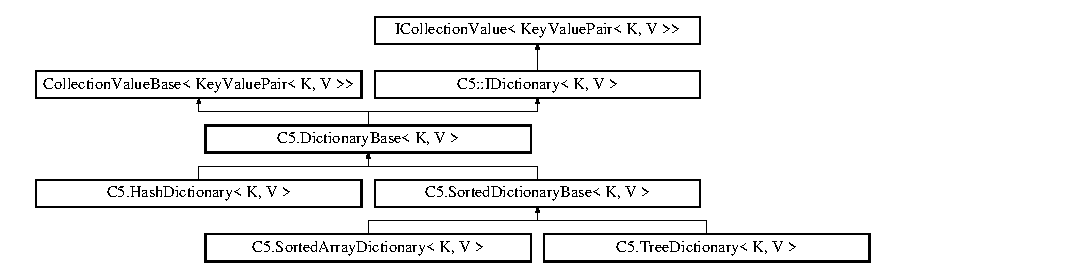
\includegraphics[height=3.286385cm]{class_c5_1_1_dictionary_base}
\end{center}
\end{figure}
\subsection*{Classes}
\begin{DoxyCompactItemize}
\item 
class {\bfseries Keys\+Collection}
\item 
class {\bfseries Values\+Collection}
\end{DoxyCompactItemize}
\subsection*{Public Member Functions}
\begin{DoxyCompactItemize}
\item 
virtual void \hyperlink{class_c5_1_1_dictionary_base_a0d7b0e8b7b2eb71b9478afac991c28b7}{Add} (K key, V value)
\begin{DoxyCompactList}\small\item\em Add a new (key, value) pair (a mapping) to the dictionary. \end{DoxyCompactList}\item 
virtual void \hyperlink{class_c5_1_1_dictionary_base_a454d6f4ea9e025def47f3105262289af}{Add\+All$<$ L, W $>$} (S\+C\+G.\+I\+Enumerable$<$ \hyperlink{struct_c5_1_1_key_value_pair}{Key\+Value\+Pair}$<$ L, W $>$$>$ entries)
\begin{DoxyCompactList}\small\item\em Add the entries from a collection of T\+:\+C5.\+Key\+Value\+Pair`2 pairs to this dictionary. \end{DoxyCompactList}\item 
virtual bool \hyperlink{class_c5_1_1_dictionary_base_aed74f70614e775dfd55a92bf7dcd94c1}{Remove} (K key)
\begin{DoxyCompactList}\small\item\em Remove an entry with a given key from the dictionary \end{DoxyCompactList}\item 
virtual bool \hyperlink{class_c5_1_1_dictionary_base_a5680ada7ac17ce609554a822af164053}{Remove} (K key, out V value)
\begin{DoxyCompactList}\small\item\em Remove an entry with a given key from the dictionary and report its value. \end{DoxyCompactList}\item 
virtual void \hyperlink{class_c5_1_1_dictionary_base_ac3a1aa92d354489522afc03f8f303087}{Clear} ()
\begin{DoxyCompactList}\small\item\em Remove all entries from the dictionary \end{DoxyCompactList}\item 
virtual bool \hyperlink{class_c5_1_1_dictionary_base_a71c99b65d5a9c3c3be9fe8c861639495}{Contains} (K key)
\begin{DoxyCompactList}\small\item\em Check if there is an entry with a specified key \end{DoxyCompactList}\item 
virtual bool \hyperlink{class_c5_1_1_dictionary_base_a7e596ed4df8b0dd9ca31545fb72c2bc3}{Contains\+All$<$ H $>$} (S\+C\+G.\+I\+Enumerable$<$ H $>$ keys)
\item 
virtual bool \hyperlink{class_c5_1_1_dictionary_base_a17d8fda8e75b7280b6ee3f5f0def2bc8}{Find} (ref K key, out V value)
\begin{DoxyCompactList}\small\item\em Check if there is an entry with a specified key and report the corresponding value if found. This can be seen as a safe form of \char`\"{}val = this\mbox{[}key\mbox{]}\char`\"{}. \end{DoxyCompactList}\item 
virtual bool \hyperlink{class_c5_1_1_dictionary_base_ad8ce6fe1f68a4c9f7be467682bb3c395}{Update} (K key, V value)
\begin{DoxyCompactList}\small\item\em Look for a specific key in the dictionary and if found replace the value with a new one. This can be seen as a non-\/adding version of \char`\"{}this\mbox{[}key\mbox{]} = val\char`\"{}. \end{DoxyCompactList}\item 
virtual bool \hyperlink{class_c5_1_1_dictionary_base_a5dce44b4a55691524ec18d59a292f902}{Update} (K key, V value, out V oldvalue)
\item 
virtual bool \hyperlink{class_c5_1_1_dictionary_base_aa0c7bfd7a2fa828f4f6ce58afba0f41e}{Find\+Or\+Add} (K key, ref V value)
\begin{DoxyCompactList}\small\item\em Look for a specific key in the dictionary. If found, report the corresponding value, else add an entry with the key and the supplied value. \end{DoxyCompactList}\item 
virtual bool \hyperlink{class_c5_1_1_dictionary_base_a6a378a34466aaf85ad45ca4c53c7b655}{Update\+Or\+Add} (K key, V value)
\begin{DoxyCompactList}\small\item\em Update value in dictionary corresponding to key if found, else add new entry. More general than \char`\"{}this\mbox{[}key\mbox{]} = val;\char`\"{} by reporting if key was found. \end{DoxyCompactList}\item 
virtual bool \hyperlink{class_c5_1_1_dictionary_base_a096aaa3cdcbb024cc90a83c5bdd69c91}{Update\+Or\+Add} (K key, V value, out V oldvalue)
\begin{DoxyCompactList}\small\item\em Update value in dictionary corresponding to key if found, else add new entry. More general than \char`\"{}this\mbox{[}key\mbox{]} = val;\char`\"{} by reporting if key was found and the old value if any. \end{DoxyCompactList}\item 
virtual bool \hyperlink{class_c5_1_1_dictionary_base_ab72061b2a1b9923c7bc7943d6276892b}{Check} ()
\begin{DoxyCompactList}\small\item\em Check the integrity of the internal data structures of this dictionary. \end{DoxyCompactList}\item 
override \hyperlink{struct_c5_1_1_key_value_pair}{Key\+Value\+Pair}$<$ K, V $>$ \hyperlink{class_c5_1_1_dictionary_base_a734231ac120be70d8144ac96e0aae0ec}{Choose} ()
\begin{DoxyCompactList}\small\item\em Choose some entry in this Dictionary. \end{DoxyCompactList}\item 
override S\+C\+G.\+I\+Enumerator$<$ \hyperlink{struct_c5_1_1_key_value_pair}{Key\+Value\+Pair}$<$ K, V $>$ $>$ \hyperlink{class_c5_1_1_dictionary_base_a6bca7a3dbc8844ea8328f39c657b60d0}{Get\+Enumerator} ()
\begin{DoxyCompactList}\small\item\em Create an enumerator for the collection of entries of the dictionary \end{DoxyCompactList}\item 
override bool \hyperlink{class_c5_1_1_dictionary_base_a1066094d2ab5ed006b436a8180907985}{Show} (System.\+Text.\+String\+Builder stringbuilder, ref int rest, I\+Format\+Provider format\+Provider)
\end{DoxyCompactItemize}
\subsection*{Protected Member Functions}
\begin{DoxyCompactItemize}
\item 
\hyperlink{class_c5_1_1_dictionary_base_a545aca28f44f72b332e605a1b30e4081}{Dictionary\+Base} (S\+C\+G.\+I\+Equality\+Comparer$<$ K $>$ keyequality\+Comparer)
\end{DoxyCompactItemize}
\subsection*{Protected Attributes}
\begin{DoxyCompactItemize}
\item 
\hyperlink{interface_c5_1_1_i_collection}{I\+Collection}$<$ \hyperlink{struct_c5_1_1_key_value_pair}{Key\+Value\+Pair}$<$ K, V $>$ $>$ \hyperlink{class_c5_1_1_dictionary_base_a05fda0813ee9609e10f80b052028debc}{pairs}
\begin{DoxyCompactList}\small\item\em The set collection of entries underlying this dictionary implementation \end{DoxyCompactList}\end{DoxyCompactItemize}
\subsection*{Properties}
\begin{DoxyCompactItemize}
\item 
override Collection\+Changed\+Handler$<$ \hyperlink{struct_c5_1_1_key_value_pair}{Key\+Value\+Pair}$<$ K, V $>$ $>$ \hyperlink{class_c5_1_1_dictionary_base_a751f335fff07b5b00a6d9a2d4bb99efa}{Collection\+Changed}
\begin{DoxyCompactList}\small\item\em The change event. Will be raised for every change operation on the collection. \end{DoxyCompactList}\item 
override Collection\+Cleared\+Handler$<$ \hyperlink{struct_c5_1_1_key_value_pair}{Key\+Value\+Pair}$<$ K, V $>$ $>$ \hyperlink{class_c5_1_1_dictionary_base_ac350f18d63173c7fea97844a5f62f461}{Collection\+Cleared}
\begin{DoxyCompactList}\small\item\em The change event. Will be raised for every change operation on the collection. \end{DoxyCompactList}\item 
override Items\+Added\+Handler$<$ \hyperlink{struct_c5_1_1_key_value_pair}{Key\+Value\+Pair}$<$ K, V $>$ $>$ \hyperlink{class_c5_1_1_dictionary_base_a3a1267cb8e0b1d260ce133d3961b2c59}{Items\+Added}
\begin{DoxyCompactList}\small\item\em The item added event. Will be raised for every individual addition to the collection. \end{DoxyCompactList}\item 
override Items\+Removed\+Handler$<$ \hyperlink{struct_c5_1_1_key_value_pair}{Key\+Value\+Pair}$<$ K, V $>$ $>$ \hyperlink{class_c5_1_1_dictionary_base_a2bdc1bb2f3e3b2024eff8f1f8710763c}{Items\+Removed}
\begin{DoxyCompactList}\small\item\em The item added event. Will be raised for every individual removal from the collection. \end{DoxyCompactList}\item 
override \hyperlink{namespace_c5_a9143bfd561fffa025d21561674758008}{Event\+Type\+Enum} \hyperlink{class_c5_1_1_dictionary_base_aa1a18f583bfe9f40a24d53b9638d1962}{Listenable\+Events}\hspace{0.3cm}{\ttfamily  \mbox{[}get\mbox{]}}
\item 
override \hyperlink{namespace_c5_a9143bfd561fffa025d21561674758008}{Event\+Type\+Enum} \hyperlink{class_c5_1_1_dictionary_base_a4ce610755137141287e684b92cdf534c}{Active\+Events}\hspace{0.3cm}{\ttfamily  \mbox{[}get\mbox{]}}
\item 
virtual S\+C\+G.\+I\+Equality\+Comparer$<$ K $>$ \hyperlink{class_c5_1_1_dictionary_base_a63cd9471d097f20096d8e3bb22fffa33}{Equality\+Comparer}\hspace{0.3cm}{\ttfamily  \mbox{[}get\mbox{]}}
\item 
virtual \hyperlink{namespace_c5_a615ba88dcdaa8d5a3c5f833a73d7fad6}{Speed} \hyperlink{class_c5_1_1_dictionary_base_ae3c0eb5e4b8a6735f4012b9a370cc769}{Contains\+Speed}\hspace{0.3cm}{\ttfamily  \mbox{[}get\mbox{]}}
\item 
virtual \hyperlink{interface_c5_1_1_i_collection_value}{I\+Collection\+Value}$<$ K $>$ \hyperlink{class_c5_1_1_dictionary_base_a42cbd2cf8d32a18b4ca17b82cf026ea5}{Keys}\hspace{0.3cm}{\ttfamily  \mbox{[}get\mbox{]}}
\item 
virtual \hyperlink{interface_c5_1_1_i_collection_value}{I\+Collection\+Value}$<$ V $>$ \hyperlink{class_c5_1_1_dictionary_base_adf392009742ab67a355c66cf423f5fe6}{Values}\hspace{0.3cm}{\ttfamily  \mbox{[}get\mbox{]}}
\item 
virtual Func$<$ K, V $>$ \hyperlink{class_c5_1_1_dictionary_base_afd227ddeb666195929f2b441b0c07bb7}{Func}\hspace{0.3cm}{\ttfamily  \mbox{[}get\mbox{]}}
\item 
virtual V \hyperlink{class_c5_1_1_dictionary_base_aca2fd266c08a8668a6f1e5b85aa43d6b}{this\mbox{[}\+K key\mbox{]}}\hspace{0.3cm}{\ttfamily  \mbox{[}get, set\mbox{]}}
\begin{DoxyCompactList}\small\item\em Indexer by key for dictionary. \end{DoxyCompactList}\item 
virtual bool \hyperlink{class_c5_1_1_dictionary_base_a12af62ed33fb01b0f103be5d4351e192}{Is\+Read\+Only}\hspace{0.3cm}{\ttfamily  \mbox{[}get\mbox{]}}
\item 
override bool \hyperlink{class_c5_1_1_dictionary_base_a6749a3f0ec6472fab5365732c66e826b}{Is\+Empty}\hspace{0.3cm}{\ttfamily  \mbox{[}get\mbox{]}}
\item 
override int \hyperlink{class_c5_1_1_dictionary_base_adcf48a45f296db6a12893ad7b13abb02}{Count}\hspace{0.3cm}{\ttfamily  \mbox{[}get\mbox{]}}
\item 
override \hyperlink{namespace_c5_a615ba88dcdaa8d5a3c5f833a73d7fad6}{Speed} \hyperlink{class_c5_1_1_dictionary_base_a6101979f24376d2e8640394e66264210}{Count\+Speed}\hspace{0.3cm}{\ttfamily  \mbox{[}get\mbox{]}}
\end{DoxyCompactItemize}


\subsection{Detailed Description}
A base class for implementing a dictionary based on a set collection implementation. {\itshape See the source code for T\+:\+C5.\+Hash\+Dictionary`2 for an example} 



\subsection{Constructor \& Destructor Documentation}
\hypertarget{class_c5_1_1_dictionary_base_a545aca28f44f72b332e605a1b30e4081}{}\index{C5\+::\+Dictionary\+Base@{C5\+::\+Dictionary\+Base}!Dictionary\+Base@{Dictionary\+Base}}
\index{Dictionary\+Base@{Dictionary\+Base}!C5\+::\+Dictionary\+Base@{C5\+::\+Dictionary\+Base}}
\subsubsection[{Dictionary\+Base(\+S\+C\+G.\+I\+Equality\+Comparer$<$ K $>$ keyequality\+Comparer)}]{\setlength{\rightskip}{0pt plus 5cm}{\bf C5.\+Dictionary\+Base}$<$ K, V $>$.{\bf Dictionary\+Base} (
\begin{DoxyParamCaption}
\item[{S\+C\+G.\+I\+Equality\+Comparer$<$ K $>$}]{keyequality\+Comparer}
\end{DoxyParamCaption}
)\hspace{0.3cm}{\ttfamily [protected]}}\label{class_c5_1_1_dictionary_base_a545aca28f44f72b332e605a1b30e4081}





\begin{DoxyParams}{Parameters}
{\em keyequality\+Comparer} & \\
\hline
\end{DoxyParams}


\subsection{Member Function Documentation}
\hypertarget{class_c5_1_1_dictionary_base_a0d7b0e8b7b2eb71b9478afac991c28b7}{}\index{C5\+::\+Dictionary\+Base@{C5\+::\+Dictionary\+Base}!Add@{Add}}
\index{Add@{Add}!C5\+::\+Dictionary\+Base@{C5\+::\+Dictionary\+Base}}
\subsubsection[{Add(\+K key, V value)}]{\setlength{\rightskip}{0pt plus 5cm}virtual void {\bf C5.\+Dictionary\+Base}$<$ K, V $>$.Add (
\begin{DoxyParamCaption}
\item[{K}]{key, }
\item[{V}]{value}
\end{DoxyParamCaption}
)\hspace{0.3cm}{\ttfamily [virtual]}}\label{class_c5_1_1_dictionary_base_a0d7b0e8b7b2eb71b9478afac991c28b7}


Add a new (key, value) pair (a mapping) to the dictionary. 


\begin{DoxyExceptions}{Exceptions}
{\em \hyperlink{class_c5_1_1_duplicate_not_allowed_exception}{Duplicate\+Not\+Allowed\+Exception}} & if there already is an entry with the same key. \\
\hline
\end{DoxyExceptions}

\begin{DoxyParams}{Parameters}
{\em key} & Key to add\\
\hline
{\em value} & Value to add\\
\hline
\end{DoxyParams}


Implements \hyperlink{interface_c5_1_1_i_dictionary_a7e3eefcf603863fe54ce86080bbc07d7}{C5.\+I\+Dictionary$<$ K, V $>$}.

\hypertarget{class_c5_1_1_dictionary_base_a454d6f4ea9e025def47f3105262289af}{}\index{C5\+::\+Dictionary\+Base@{C5\+::\+Dictionary\+Base}!Add\+All$<$ L, W $>$@{Add\+All$<$ L, W $>$}}
\index{Add\+All$<$ L, W $>$@{Add\+All$<$ L, W $>$}!C5\+::\+Dictionary\+Base@{C5\+::\+Dictionary\+Base}}
\subsubsection[{Add\+All$<$ L, W $>$(\+S\+C\+G.\+I\+Enumerable$<$ Key\+Value\+Pair$<$ L, W $>$$>$ entries)}]{\setlength{\rightskip}{0pt plus 5cm}virtual void {\bf C5.\+Dictionary\+Base}$<$ K, V $>$.Add\+All$<$ L, W $>$ (
\begin{DoxyParamCaption}
\item[{S\+C\+G.\+I\+Enumerable$<$ {\bf Key\+Value\+Pair}$<$ L, W $>$$>$}]{entries}
\end{DoxyParamCaption}
)\hspace{0.3cm}{\ttfamily [virtual]}}\label{class_c5_1_1_dictionary_base_a454d6f4ea9e025def47f3105262289af}


Add the entries from a collection of T\+:\+C5.\+Key\+Value\+Pair`2 pairs to this dictionary. 

{\bfseries T\+O\+D\+O\+: add restrictions L\+:K and W\+:V when the .Net S\+D\+K allows it }


\begin{DoxyExceptions}{Exceptions}
{\em \hyperlink{class_c5_1_1_duplicate_not_allowed_exception}{Duplicate\+Not\+Allowed\+Exception}} & If the input contains duplicate keys or a key already present in this dictionary.\\
\hline
\end{DoxyExceptions}

\begin{DoxyParams}{Parameters}
{\em entries} & \\
\hline
\end{DoxyParams}
\begin{Desc}
\item[Type Constraints]\begin{description}
\item[{\em L} : {\em K}]\item[{\em W} : {\em V}]\end{description}
\end{Desc}
\hypertarget{class_c5_1_1_dictionary_base_ab72061b2a1b9923c7bc7943d6276892b}{}\index{C5\+::\+Dictionary\+Base@{C5\+::\+Dictionary\+Base}!Check@{Check}}
\index{Check@{Check}!C5\+::\+Dictionary\+Base@{C5\+::\+Dictionary\+Base}}
\subsubsection[{Check()}]{\setlength{\rightskip}{0pt plus 5cm}virtual bool {\bf C5.\+Dictionary\+Base}$<$ K, V $>$.Check (
\begin{DoxyParamCaption}
{}
\end{DoxyParamCaption}
)\hspace{0.3cm}{\ttfamily [virtual]}}\label{class_c5_1_1_dictionary_base_ab72061b2a1b9923c7bc7943d6276892b}


Check the integrity of the internal data structures of this dictionary. 

\begin{DoxyReturn}{Returns}
True if check does not fail.
\end{DoxyReturn}


Implements \hyperlink{interface_c5_1_1_i_dictionary_a659969044740981cdcfe5ee86585104c}{C5.\+I\+Dictionary$<$ K, V $>$}.

\hypertarget{class_c5_1_1_dictionary_base_a734231ac120be70d8144ac96e0aae0ec}{}\index{C5\+::\+Dictionary\+Base@{C5\+::\+Dictionary\+Base}!Choose@{Choose}}
\index{Choose@{Choose}!C5\+::\+Dictionary\+Base@{C5\+::\+Dictionary\+Base}}
\subsubsection[{Choose()}]{\setlength{\rightskip}{0pt plus 5cm}override {\bf Key\+Value\+Pair}$<$K, V$>$ {\bf C5.\+Dictionary\+Base}$<$ K, V $>$.Choose (
\begin{DoxyParamCaption}
{}
\end{DoxyParamCaption}
)}\label{class_c5_1_1_dictionary_base_a734231ac120be70d8144ac96e0aae0ec}


Choose some entry in this Dictionary. 


\begin{DoxyExceptions}{Exceptions}
{\em \hyperlink{class_c5_1_1_no_such_item_exception}{No\+Such\+Item\+Exception}} & if collection is empty.\\
\hline
\end{DoxyExceptions}
\begin{DoxyReturn}{Returns}

\end{DoxyReturn}
\hypertarget{class_c5_1_1_dictionary_base_ac3a1aa92d354489522afc03f8f303087}{}\index{C5\+::\+Dictionary\+Base@{C5\+::\+Dictionary\+Base}!Clear@{Clear}}
\index{Clear@{Clear}!C5\+::\+Dictionary\+Base@{C5\+::\+Dictionary\+Base}}
\subsubsection[{Clear()}]{\setlength{\rightskip}{0pt plus 5cm}virtual void {\bf C5.\+Dictionary\+Base}$<$ K, V $>$.Clear (
\begin{DoxyParamCaption}
{}
\end{DoxyParamCaption}
)\hspace{0.3cm}{\ttfamily [virtual]}}\label{class_c5_1_1_dictionary_base_ac3a1aa92d354489522afc03f8f303087}


Remove all entries from the dictionary 



Implements \hyperlink{interface_c5_1_1_i_dictionary_a9eb0026921a6b39c781495efd65dc82b}{C5.\+I\+Dictionary$<$ K, V $>$}.

\hypertarget{class_c5_1_1_dictionary_base_a71c99b65d5a9c3c3be9fe8c861639495}{}\index{C5\+::\+Dictionary\+Base@{C5\+::\+Dictionary\+Base}!Contains@{Contains}}
\index{Contains@{Contains}!C5\+::\+Dictionary\+Base@{C5\+::\+Dictionary\+Base}}
\subsubsection[{Contains(\+K key)}]{\setlength{\rightskip}{0pt plus 5cm}virtual bool {\bf C5.\+Dictionary\+Base}$<$ K, V $>$.Contains (
\begin{DoxyParamCaption}
\item[{K}]{key}
\end{DoxyParamCaption}
)\hspace{0.3cm}{\ttfamily [virtual]}}\label{class_c5_1_1_dictionary_base_a71c99b65d5a9c3c3be9fe8c861639495}


Check if there is an entry with a specified key 


\begin{DoxyParams}{Parameters}
{\em key} & The key to look for\\
\hline
\end{DoxyParams}
\begin{DoxyReturn}{Returns}
True if key was found
\end{DoxyReturn}


Implements \hyperlink{interface_c5_1_1_i_dictionary_a08f4af4a7f427e8e9022a13f2e79c031}{C5.\+I\+Dictionary$<$ K, V $>$}.

\hypertarget{class_c5_1_1_dictionary_base_a7e596ed4df8b0dd9ca31545fb72c2bc3}{}\index{C5\+::\+Dictionary\+Base@{C5\+::\+Dictionary\+Base}!Contains\+All$<$ H $>$@{Contains\+All$<$ H $>$}}
\index{Contains\+All$<$ H $>$@{Contains\+All$<$ H $>$}!C5\+::\+Dictionary\+Base@{C5\+::\+Dictionary\+Base}}
\subsubsection[{Contains\+All$<$ H $>$(\+S\+C\+G.\+I\+Enumerable$<$ H $>$ keys)}]{\setlength{\rightskip}{0pt plus 5cm}virtual bool {\bf C5.\+Dictionary\+Base}$<$ K, V $>$.Contains\+All$<$ H $>$ (
\begin{DoxyParamCaption}
\item[{S\+C\+G.\+I\+Enumerable$<$ H $>$}]{keys}
\end{DoxyParamCaption}
)\hspace{0.3cm}{\ttfamily [virtual]}}\label{class_c5_1_1_dictionary_base_a7e596ed4df8b0dd9ca31545fb72c2bc3}





\begin{DoxyParams}{Parameters}
{\em keys} & \\
\hline
\end{DoxyParams}
\begin{DoxyReturn}{Returns}

\end{DoxyReturn}


Implements \hyperlink{interface_c5_1_1_i_dictionary_a18a33ccf0bac3ac7ef8046850104c5d5}{C5.\+I\+Dictionary$<$ K, V $>$}.

\begin{Desc}
\item[Type Constraints]\begin{description}
\item[{\em H} : {\em K}]\end{description}
\end{Desc}
\hypertarget{class_c5_1_1_dictionary_base_a17d8fda8e75b7280b6ee3f5f0def2bc8}{}\index{C5\+::\+Dictionary\+Base@{C5\+::\+Dictionary\+Base}!Find@{Find}}
\index{Find@{Find}!C5\+::\+Dictionary\+Base@{C5\+::\+Dictionary\+Base}}
\subsubsection[{Find(ref K key, out V value)}]{\setlength{\rightskip}{0pt plus 5cm}virtual bool {\bf C5.\+Dictionary\+Base}$<$ K, V $>$.Find (
\begin{DoxyParamCaption}
\item[{ref K}]{key, }
\item[{out V}]{value}
\end{DoxyParamCaption}
)\hspace{0.3cm}{\ttfamily [virtual]}}\label{class_c5_1_1_dictionary_base_a17d8fda8e75b7280b6ee3f5f0def2bc8}


Check if there is an entry with a specified key and report the corresponding value if found. This can be seen as a safe form of \char`\"{}val = this\mbox{[}key\mbox{]}\char`\"{}. 


\begin{DoxyParams}{Parameters}
{\em key} & The key to look for\\
\hline
{\em value} & On exit, the value of the entry\\
\hline
\end{DoxyParams}
\begin{DoxyReturn}{Returns}
True if key was found
\end{DoxyReturn}


Implements \hyperlink{interface_c5_1_1_i_dictionary_a40f6257961c1578fea31f0507cd5c28e}{C5.\+I\+Dictionary$<$ K, V $>$}.

\hypertarget{class_c5_1_1_dictionary_base_aa0c7bfd7a2fa828f4f6ce58afba0f41e}{}\index{C5\+::\+Dictionary\+Base@{C5\+::\+Dictionary\+Base}!Find\+Or\+Add@{Find\+Or\+Add}}
\index{Find\+Or\+Add@{Find\+Or\+Add}!C5\+::\+Dictionary\+Base@{C5\+::\+Dictionary\+Base}}
\subsubsection[{Find\+Or\+Add(\+K key, ref V value)}]{\setlength{\rightskip}{0pt plus 5cm}virtual bool {\bf C5.\+Dictionary\+Base}$<$ K, V $>$.Find\+Or\+Add (
\begin{DoxyParamCaption}
\item[{K}]{key, }
\item[{ref V}]{value}
\end{DoxyParamCaption}
)\hspace{0.3cm}{\ttfamily [virtual]}}\label{class_c5_1_1_dictionary_base_aa0c7bfd7a2fa828f4f6ce58afba0f41e}


Look for a specific key in the dictionary. If found, report the corresponding value, else add an entry with the key and the supplied value. 


\begin{DoxyParams}{Parameters}
{\em key} & On entry the key to look for\\
\hline
{\em value} & On entry the value to add if the key is not found. On exit the value found if any.\\
\hline
\end{DoxyParams}
\begin{DoxyReturn}{Returns}
True if key was found
\end{DoxyReturn}


Implements \hyperlink{interface_c5_1_1_i_dictionary_a1f9f0bd335980be8c24d74470bd19ffc}{C5.\+I\+Dictionary$<$ K, V $>$}.

\hypertarget{class_c5_1_1_dictionary_base_a6bca7a3dbc8844ea8328f39c657b60d0}{}\index{C5\+::\+Dictionary\+Base@{C5\+::\+Dictionary\+Base}!Get\+Enumerator@{Get\+Enumerator}}
\index{Get\+Enumerator@{Get\+Enumerator}!C5\+::\+Dictionary\+Base@{C5\+::\+Dictionary\+Base}}
\subsubsection[{Get\+Enumerator()}]{\setlength{\rightskip}{0pt plus 5cm}override S\+C\+G.\+I\+Enumerator$<${\bf Key\+Value\+Pair}$<$K, V$>$ $>$ {\bf C5.\+Dictionary\+Base}$<$ K, V $>$.Get\+Enumerator (
\begin{DoxyParamCaption}
{}
\end{DoxyParamCaption}
)}\label{class_c5_1_1_dictionary_base_a6bca7a3dbc8844ea8328f39c657b60d0}


Create an enumerator for the collection of entries of the dictionary 

\begin{DoxyReturn}{Returns}
The enumerator
\end{DoxyReturn}
\hypertarget{class_c5_1_1_dictionary_base_aed74f70614e775dfd55a92bf7dcd94c1}{}\index{C5\+::\+Dictionary\+Base@{C5\+::\+Dictionary\+Base}!Remove@{Remove}}
\index{Remove@{Remove}!C5\+::\+Dictionary\+Base@{C5\+::\+Dictionary\+Base}}
\subsubsection[{Remove(\+K key)}]{\setlength{\rightskip}{0pt plus 5cm}virtual bool {\bf C5.\+Dictionary\+Base}$<$ K, V $>$.Remove (
\begin{DoxyParamCaption}
\item[{K}]{key}
\end{DoxyParamCaption}
)\hspace{0.3cm}{\ttfamily [virtual]}}\label{class_c5_1_1_dictionary_base_aed74f70614e775dfd55a92bf7dcd94c1}


Remove an entry with a given key from the dictionary 


\begin{DoxyParams}{Parameters}
{\em key} & The key of the entry to remove\\
\hline
\end{DoxyParams}
\begin{DoxyReturn}{Returns}
True if an entry was found (and removed)
\end{DoxyReturn}


Implements \hyperlink{interface_c5_1_1_i_dictionary_a35b1f0b9f0e0c555246b9154b6e45ab5}{C5.\+I\+Dictionary$<$ K, V $>$}.

\hypertarget{class_c5_1_1_dictionary_base_a5680ada7ac17ce609554a822af164053}{}\index{C5\+::\+Dictionary\+Base@{C5\+::\+Dictionary\+Base}!Remove@{Remove}}
\index{Remove@{Remove}!C5\+::\+Dictionary\+Base@{C5\+::\+Dictionary\+Base}}
\subsubsection[{Remove(\+K key, out V value)}]{\setlength{\rightskip}{0pt plus 5cm}virtual bool {\bf C5.\+Dictionary\+Base}$<$ K, V $>$.Remove (
\begin{DoxyParamCaption}
\item[{K}]{key, }
\item[{out V}]{value}
\end{DoxyParamCaption}
)\hspace{0.3cm}{\ttfamily [virtual]}}\label{class_c5_1_1_dictionary_base_a5680ada7ac17ce609554a822af164053}


Remove an entry with a given key from the dictionary and report its value. 


\begin{DoxyParams}{Parameters}
{\em key} & The key of the entry to remove\\
\hline
{\em value} & On exit, the value of the removed entry\\
\hline
\end{DoxyParams}
\begin{DoxyReturn}{Returns}
True if an entry was found (and removed)
\end{DoxyReturn}


Implements \hyperlink{interface_c5_1_1_i_dictionary_a24f34aa709dc1157536afb1d251135d5}{C5.\+I\+Dictionary$<$ K, V $>$}.

\hypertarget{class_c5_1_1_dictionary_base_a1066094d2ab5ed006b436a8180907985}{}\index{C5\+::\+Dictionary\+Base@{C5\+::\+Dictionary\+Base}!Show@{Show}}
\index{Show@{Show}!C5\+::\+Dictionary\+Base@{C5\+::\+Dictionary\+Base}}
\subsubsection[{Show(\+System.\+Text.\+String\+Builder stringbuilder, ref int rest, I\+Format\+Provider format\+Provider)}]{\setlength{\rightskip}{0pt plus 5cm}override bool {\bf C5.\+Dictionary\+Base}$<$ K, V $>$.Show (
\begin{DoxyParamCaption}
\item[{System.\+Text.\+String\+Builder}]{stringbuilder, }
\item[{ref int}]{rest, }
\item[{I\+Format\+Provider}]{format\+Provider}
\end{DoxyParamCaption}
)}\label{class_c5_1_1_dictionary_base_a1066094d2ab5ed006b436a8180907985}





\begin{DoxyParams}{Parameters}
{\em stringbuilder} & \\
\hline
{\em rest} & \\
\hline
{\em format\+Provider} & \\
\hline
\end{DoxyParams}
\begin{DoxyReturn}{Returns}

\end{DoxyReturn}
\hypertarget{class_c5_1_1_dictionary_base_ad8ce6fe1f68a4c9f7be467682bb3c395}{}\index{C5\+::\+Dictionary\+Base@{C5\+::\+Dictionary\+Base}!Update@{Update}}
\index{Update@{Update}!C5\+::\+Dictionary\+Base@{C5\+::\+Dictionary\+Base}}
\subsubsection[{Update(\+K key, V value)}]{\setlength{\rightskip}{0pt plus 5cm}virtual bool {\bf C5.\+Dictionary\+Base}$<$ K, V $>$.Update (
\begin{DoxyParamCaption}
\item[{K}]{key, }
\item[{V}]{value}
\end{DoxyParamCaption}
)\hspace{0.3cm}{\ttfamily [virtual]}}\label{class_c5_1_1_dictionary_base_ad8ce6fe1f68a4c9f7be467682bb3c395}


Look for a specific key in the dictionary and if found replace the value with a new one. This can be seen as a non-\/adding version of \char`\"{}this\mbox{[}key\mbox{]} = val\char`\"{}. 


\begin{DoxyParams}{Parameters}
{\em key} & The key to look for\\
\hline
{\em value} & The new value\\
\hline
\end{DoxyParams}
\begin{DoxyReturn}{Returns}
True if key was found
\end{DoxyReturn}


Implements \hyperlink{interface_c5_1_1_i_dictionary_aa1af112490cca3ed7816d47b9127dace}{C5.\+I\+Dictionary$<$ K, V $>$}.

\hypertarget{class_c5_1_1_dictionary_base_a5dce44b4a55691524ec18d59a292f902}{}\index{C5\+::\+Dictionary\+Base@{C5\+::\+Dictionary\+Base}!Update@{Update}}
\index{Update@{Update}!C5\+::\+Dictionary\+Base@{C5\+::\+Dictionary\+Base}}
\subsubsection[{Update(\+K key, V value, out V oldvalue)}]{\setlength{\rightskip}{0pt plus 5cm}virtual bool {\bf C5.\+Dictionary\+Base}$<$ K, V $>$.Update (
\begin{DoxyParamCaption}
\item[{K}]{key, }
\item[{V}]{value, }
\item[{out V}]{oldvalue}
\end{DoxyParamCaption}
)\hspace{0.3cm}{\ttfamily [virtual]}}\label{class_c5_1_1_dictionary_base_a5dce44b4a55691524ec18d59a292f902}





\begin{DoxyParams}{Parameters}
{\em key} & \\
\hline
{\em value} & \\
\hline
{\em oldvalue} & \\
\hline
\end{DoxyParams}
\begin{DoxyReturn}{Returns}

\end{DoxyReturn}


Implements \hyperlink{interface_c5_1_1_i_dictionary_a0338a7b5bfa797aeb75d153faf00dc31}{C5.\+I\+Dictionary$<$ K, V $>$}.

\hypertarget{class_c5_1_1_dictionary_base_a6a378a34466aaf85ad45ca4c53c7b655}{}\index{C5\+::\+Dictionary\+Base@{C5\+::\+Dictionary\+Base}!Update\+Or\+Add@{Update\+Or\+Add}}
\index{Update\+Or\+Add@{Update\+Or\+Add}!C5\+::\+Dictionary\+Base@{C5\+::\+Dictionary\+Base}}
\subsubsection[{Update\+Or\+Add(\+K key, V value)}]{\setlength{\rightskip}{0pt plus 5cm}virtual bool {\bf C5.\+Dictionary\+Base}$<$ K, V $>$.Update\+Or\+Add (
\begin{DoxyParamCaption}
\item[{K}]{key, }
\item[{V}]{value}
\end{DoxyParamCaption}
)\hspace{0.3cm}{\ttfamily [virtual]}}\label{class_c5_1_1_dictionary_base_a6a378a34466aaf85ad45ca4c53c7b655}


Update value in dictionary corresponding to key if found, else add new entry. More general than \char`\"{}this\mbox{[}key\mbox{]} = val;\char`\"{} by reporting if key was found. 


\begin{DoxyParams}{Parameters}
{\em key} & The key to look for\\
\hline
{\em value} & The value to add or replace with.\\
\hline
\end{DoxyParams}
\begin{DoxyReturn}{Returns}
True if entry was updated.
\end{DoxyReturn}


Implements \hyperlink{interface_c5_1_1_i_dictionary_a9cb26d974f4da6030fe50b4bcc3dc4f1}{C5.\+I\+Dictionary$<$ K, V $>$}.

\hypertarget{class_c5_1_1_dictionary_base_a096aaa3cdcbb024cc90a83c5bdd69c91}{}\index{C5\+::\+Dictionary\+Base@{C5\+::\+Dictionary\+Base}!Update\+Or\+Add@{Update\+Or\+Add}}
\index{Update\+Or\+Add@{Update\+Or\+Add}!C5\+::\+Dictionary\+Base@{C5\+::\+Dictionary\+Base}}
\subsubsection[{Update\+Or\+Add(\+K key, V value, out V oldvalue)}]{\setlength{\rightskip}{0pt plus 5cm}virtual bool {\bf C5.\+Dictionary\+Base}$<$ K, V $>$.Update\+Or\+Add (
\begin{DoxyParamCaption}
\item[{K}]{key, }
\item[{V}]{value, }
\item[{out V}]{oldvalue}
\end{DoxyParamCaption}
)\hspace{0.3cm}{\ttfamily [virtual]}}\label{class_c5_1_1_dictionary_base_a096aaa3cdcbb024cc90a83c5bdd69c91}


Update value in dictionary corresponding to key if found, else add new entry. More general than \char`\"{}this\mbox{[}key\mbox{]} = val;\char`\"{} by reporting if key was found and the old value if any. 


\begin{DoxyParams}{Parameters}
{\em key} & \\
\hline
{\em value} & \\
\hline
{\em oldvalue} & \\
\hline
\end{DoxyParams}
\begin{DoxyReturn}{Returns}

\end{DoxyReturn}


Implements \hyperlink{interface_c5_1_1_i_dictionary_abc8d5a032bbf487db18fc26e31ad512d}{C5.\+I\+Dictionary$<$ K, V $>$}.



\subsection{Member Data Documentation}
\hypertarget{class_c5_1_1_dictionary_base_a05fda0813ee9609e10f80b052028debc}{}\index{C5\+::\+Dictionary\+Base@{C5\+::\+Dictionary\+Base}!pairs@{pairs}}
\index{pairs@{pairs}!C5\+::\+Dictionary\+Base@{C5\+::\+Dictionary\+Base}}
\subsubsection[{pairs}]{\setlength{\rightskip}{0pt plus 5cm}{\bf I\+Collection}$<${\bf Key\+Value\+Pair}$<$K, V$>$ $>$ {\bf C5.\+Dictionary\+Base}$<$ K, V $>$.pairs\hspace{0.3cm}{\ttfamily [protected]}}\label{class_c5_1_1_dictionary_base_a05fda0813ee9609e10f80b052028debc}


The set collection of entries underlying this dictionary implementation 



\subsection{Property Documentation}
\hypertarget{class_c5_1_1_dictionary_base_a4ce610755137141287e684b92cdf534c}{}\index{C5\+::\+Dictionary\+Base@{C5\+::\+Dictionary\+Base}!Active\+Events@{Active\+Events}}
\index{Active\+Events@{Active\+Events}!C5\+::\+Dictionary\+Base@{C5\+::\+Dictionary\+Base}}
\subsubsection[{Active\+Events}]{\setlength{\rightskip}{0pt plus 5cm}override {\bf Event\+Type\+Enum} {\bf C5.\+Dictionary\+Base}$<$ K, V $>$.Active\+Events\hspace{0.3cm}{\ttfamily [get]}}\label{class_c5_1_1_dictionary_base_a4ce610755137141287e684b92cdf534c}




\hypertarget{class_c5_1_1_dictionary_base_a751f335fff07b5b00a6d9a2d4bb99efa}{}\index{C5\+::\+Dictionary\+Base@{C5\+::\+Dictionary\+Base}!Collection\+Changed@{Collection\+Changed}}
\index{Collection\+Changed@{Collection\+Changed}!C5\+::\+Dictionary\+Base@{C5\+::\+Dictionary\+Base}}
\subsubsection[{Collection\+Changed}]{\setlength{\rightskip}{0pt plus 5cm}override Collection\+Changed\+Handler$<${\bf Key\+Value\+Pair}$<$K, V$>$ $>$ {\bf C5.\+Dictionary\+Base}$<$ K, V $>$.Collection\+Changed\hspace{0.3cm}{\ttfamily [add]}, {\ttfamily [remove]}}\label{class_c5_1_1_dictionary_base_a751f335fff07b5b00a6d9a2d4bb99efa}


The change event. Will be raised for every change operation on the collection. 

\hypertarget{class_c5_1_1_dictionary_base_ac350f18d63173c7fea97844a5f62f461}{}\index{C5\+::\+Dictionary\+Base@{C5\+::\+Dictionary\+Base}!Collection\+Cleared@{Collection\+Cleared}}
\index{Collection\+Cleared@{Collection\+Cleared}!C5\+::\+Dictionary\+Base@{C5\+::\+Dictionary\+Base}}
\subsubsection[{Collection\+Cleared}]{\setlength{\rightskip}{0pt plus 5cm}override Collection\+Cleared\+Handler$<${\bf Key\+Value\+Pair}$<$K, V$>$ $>$ {\bf C5.\+Dictionary\+Base}$<$ K, V $>$.Collection\+Cleared\hspace{0.3cm}{\ttfamily [add]}, {\ttfamily [remove]}}\label{class_c5_1_1_dictionary_base_ac350f18d63173c7fea97844a5f62f461}


The change event. Will be raised for every change operation on the collection. 

\hypertarget{class_c5_1_1_dictionary_base_ae3c0eb5e4b8a6735f4012b9a370cc769}{}\index{C5\+::\+Dictionary\+Base@{C5\+::\+Dictionary\+Base}!Contains\+Speed@{Contains\+Speed}}
\index{Contains\+Speed@{Contains\+Speed}!C5\+::\+Dictionary\+Base@{C5\+::\+Dictionary\+Base}}
\subsubsection[{Contains\+Speed}]{\setlength{\rightskip}{0pt plus 5cm}virtual {\bf Speed} {\bf C5.\+Dictionary\+Base}$<$ K, V $>$.Contains\+Speed\hspace{0.3cm}{\ttfamily [get]}}\label{class_c5_1_1_dictionary_base_ae3c0eb5e4b8a6735f4012b9a370cc769}




\hypertarget{class_c5_1_1_dictionary_base_adcf48a45f296db6a12893ad7b13abb02}{}\index{C5\+::\+Dictionary\+Base@{C5\+::\+Dictionary\+Base}!Count@{Count}}
\index{Count@{Count}!C5\+::\+Dictionary\+Base@{C5\+::\+Dictionary\+Base}}
\subsubsection[{Count}]{\setlength{\rightskip}{0pt plus 5cm}override int {\bf C5.\+Dictionary\+Base}$<$ K, V $>$.Count\hspace{0.3cm}{\ttfamily [get]}}\label{class_c5_1_1_dictionary_base_adcf48a45f296db6a12893ad7b13abb02}




The number of entrues in the dictionary\hypertarget{class_c5_1_1_dictionary_base_a6101979f24376d2e8640394e66264210}{}\index{C5\+::\+Dictionary\+Base@{C5\+::\+Dictionary\+Base}!Count\+Speed@{Count\+Speed}}
\index{Count\+Speed@{Count\+Speed}!C5\+::\+Dictionary\+Base@{C5\+::\+Dictionary\+Base}}
\subsubsection[{Count\+Speed}]{\setlength{\rightskip}{0pt plus 5cm}override {\bf Speed} {\bf C5.\+Dictionary\+Base}$<$ K, V $>$.Count\+Speed\hspace{0.3cm}{\ttfamily [get]}}\label{class_c5_1_1_dictionary_base_a6101979f24376d2e8640394e66264210}




The number of entrues in the dictionary\hypertarget{class_c5_1_1_dictionary_base_a63cd9471d097f20096d8e3bb22fffa33}{}\index{C5\+::\+Dictionary\+Base@{C5\+::\+Dictionary\+Base}!Equality\+Comparer@{Equality\+Comparer}}
\index{Equality\+Comparer@{Equality\+Comparer}!C5\+::\+Dictionary\+Base@{C5\+::\+Dictionary\+Base}}
\subsubsection[{Equality\+Comparer}]{\setlength{\rightskip}{0pt plus 5cm}virtual S\+C\+G.\+I\+Equality\+Comparer$<$K$>$ {\bf C5.\+Dictionary\+Base}$<$ K, V $>$.Equality\+Comparer\hspace{0.3cm}{\ttfamily [get]}}\label{class_c5_1_1_dictionary_base_a63cd9471d097f20096d8e3bb22fffa33}




\hypertarget{class_c5_1_1_dictionary_base_afd227ddeb666195929f2b441b0c07bb7}{}\index{C5\+::\+Dictionary\+Base@{C5\+::\+Dictionary\+Base}!Func@{Func}}
\index{Func@{Func}!C5\+::\+Dictionary\+Base@{C5\+::\+Dictionary\+Base}}
\subsubsection[{Func}]{\setlength{\rightskip}{0pt plus 5cm}virtual Func$<$K, V$>$ {\bf C5.\+Dictionary\+Base}$<$ K, V $>$.Func\hspace{0.3cm}{\ttfamily [get]}}\label{class_c5_1_1_dictionary_base_afd227ddeb666195929f2b441b0c07bb7}




\hypertarget{class_c5_1_1_dictionary_base_a6749a3f0ec6472fab5365732c66e826b}{}\index{C5\+::\+Dictionary\+Base@{C5\+::\+Dictionary\+Base}!Is\+Empty@{Is\+Empty}}
\index{Is\+Empty@{Is\+Empty}!C5\+::\+Dictionary\+Base@{C5\+::\+Dictionary\+Base}}
\subsubsection[{Is\+Empty}]{\setlength{\rightskip}{0pt plus 5cm}override bool {\bf C5.\+Dictionary\+Base}$<$ K, V $>$.Is\+Empty\hspace{0.3cm}{\ttfamily [get]}}\label{class_c5_1_1_dictionary_base_a6749a3f0ec6472fab5365732c66e826b}




True if this collection is empty.\hypertarget{class_c5_1_1_dictionary_base_a12af62ed33fb01b0f103be5d4351e192}{}\index{C5\+::\+Dictionary\+Base@{C5\+::\+Dictionary\+Base}!Is\+Read\+Only@{Is\+Read\+Only}}
\index{Is\+Read\+Only@{Is\+Read\+Only}!C5\+::\+Dictionary\+Base@{C5\+::\+Dictionary\+Base}}
\subsubsection[{Is\+Read\+Only}]{\setlength{\rightskip}{0pt plus 5cm}virtual bool {\bf C5.\+Dictionary\+Base}$<$ K, V $>$.Is\+Read\+Only\hspace{0.3cm}{\ttfamily [get]}}\label{class_c5_1_1_dictionary_base_a12af62ed33fb01b0f103be5d4351e192}




True if dictionary is read only\hypertarget{class_c5_1_1_dictionary_base_a3a1267cb8e0b1d260ce133d3961b2c59}{}\index{C5\+::\+Dictionary\+Base@{C5\+::\+Dictionary\+Base}!Items\+Added@{Items\+Added}}
\index{Items\+Added@{Items\+Added}!C5\+::\+Dictionary\+Base@{C5\+::\+Dictionary\+Base}}
\subsubsection[{Items\+Added}]{\setlength{\rightskip}{0pt plus 5cm}override Items\+Added\+Handler$<${\bf Key\+Value\+Pair}$<$K, V$>$ $>$ {\bf C5.\+Dictionary\+Base}$<$ K, V $>$.Items\+Added\hspace{0.3cm}{\ttfamily [add]}, {\ttfamily [remove]}}\label{class_c5_1_1_dictionary_base_a3a1267cb8e0b1d260ce133d3961b2c59}


The item added event. Will be raised for every individual addition to the collection. 

\hypertarget{class_c5_1_1_dictionary_base_a2bdc1bb2f3e3b2024eff8f1f8710763c}{}\index{C5\+::\+Dictionary\+Base@{C5\+::\+Dictionary\+Base}!Items\+Removed@{Items\+Removed}}
\index{Items\+Removed@{Items\+Removed}!C5\+::\+Dictionary\+Base@{C5\+::\+Dictionary\+Base}}
\subsubsection[{Items\+Removed}]{\setlength{\rightskip}{0pt plus 5cm}override Items\+Removed\+Handler$<${\bf Key\+Value\+Pair}$<$K, V$>$ $>$ {\bf C5.\+Dictionary\+Base}$<$ K, V $>$.Items\+Removed\hspace{0.3cm}{\ttfamily [add]}, {\ttfamily [remove]}}\label{class_c5_1_1_dictionary_base_a2bdc1bb2f3e3b2024eff8f1f8710763c}


The item added event. Will be raised for every individual removal from the collection. 

\hypertarget{class_c5_1_1_dictionary_base_a42cbd2cf8d32a18b4ca17b82cf026ea5}{}\index{C5\+::\+Dictionary\+Base@{C5\+::\+Dictionary\+Base}!Keys@{Keys}}
\index{Keys@{Keys}!C5\+::\+Dictionary\+Base@{C5\+::\+Dictionary\+Base}}
\subsubsection[{Keys}]{\setlength{\rightskip}{0pt plus 5cm}virtual {\bf I\+Collection\+Value}$<$K$>$ {\bf C5.\+Dictionary\+Base}$<$ K, V $>$.Keys\hspace{0.3cm}{\ttfamily [get]}}\label{class_c5_1_1_dictionary_base_a42cbd2cf8d32a18b4ca17b82cf026ea5}




A collection containg the all the keys of the dictionary\hypertarget{class_c5_1_1_dictionary_base_aa1a18f583bfe9f40a24d53b9638d1962}{}\index{C5\+::\+Dictionary\+Base@{C5\+::\+Dictionary\+Base}!Listenable\+Events@{Listenable\+Events}}
\index{Listenable\+Events@{Listenable\+Events}!C5\+::\+Dictionary\+Base@{C5\+::\+Dictionary\+Base}}
\subsubsection[{Listenable\+Events}]{\setlength{\rightskip}{0pt plus 5cm}override {\bf Event\+Type\+Enum} {\bf C5.\+Dictionary\+Base}$<$ K, V $>$.Listenable\+Events\hspace{0.3cm}{\ttfamily [get]}}\label{class_c5_1_1_dictionary_base_aa1a18f583bfe9f40a24d53b9638d1962}




\hypertarget{class_c5_1_1_dictionary_base_aca2fd266c08a8668a6f1e5b85aa43d6b}{}\index{C5\+::\+Dictionary\+Base@{C5\+::\+Dictionary\+Base}!this\mbox{[}\+K key\mbox{]}@{this[K key]}}
\index{this\mbox{[}\+K key\mbox{]}@{this[K key]}!C5\+::\+Dictionary\+Base@{C5\+::\+Dictionary\+Base}}
\subsubsection[{this[K key]}]{\setlength{\rightskip}{0pt plus 5cm}virtual V {\bf C5.\+Dictionary\+Base}$<$ K, V $>$.this\mbox{[}K key\mbox{]}\hspace{0.3cm}{\ttfamily [get]}, {\ttfamily [set]}}\label{class_c5_1_1_dictionary_base_aca2fd266c08a8668a6f1e5b85aa43d6b}


Indexer by key for dictionary. 

The get method will throw an exception if no entry is found. 

The set method behaves like M\+:\+C5.\+Dictionary\+Base`2.\+Update\+Or\+Add(`0,`1).


\begin{DoxyExceptions}{Exceptions}
{\em \hyperlink{class_c5_1_1_no_such_item_exception}{No\+Such\+Item\+Exception}} & On get if no entry is found. \\
\hline
\end{DoxyExceptions}


The value corresponding to the key\hypertarget{class_c5_1_1_dictionary_base_adf392009742ab67a355c66cf423f5fe6}{}\index{C5\+::\+Dictionary\+Base@{C5\+::\+Dictionary\+Base}!Values@{Values}}
\index{Values@{Values}!C5\+::\+Dictionary\+Base@{C5\+::\+Dictionary\+Base}}
\subsubsection[{Values}]{\setlength{\rightskip}{0pt plus 5cm}virtual {\bf I\+Collection\+Value}$<$V$>$ {\bf C5.\+Dictionary\+Base}$<$ K, V $>$.Values\hspace{0.3cm}{\ttfamily [get]}}\label{class_c5_1_1_dictionary_base_adf392009742ab67a355c66cf423f5fe6}




A collection containing all the values of the dictionary

The documentation for this class was generated from the following file\+:\begin{DoxyCompactItemize}
\item 
C\+:/\+Users/rasmusl/\+Source/\+Repos/\+C5/\+C5/\hyperlink{_dictionaries_8cs}{Dictionaries.\+cs}\end{DoxyCompactItemize}

\hypertarget{class_c5_1_1_directed_collection_base}{}\section{C5.\+Directed\+Collection\+Base$<$ T $>$ Class Template Reference}
\label{class_c5_1_1_directed_collection_base}\index{C5.\+Directed\+Collection\+Base$<$ T $>$@{C5.\+Directed\+Collection\+Base$<$ T $>$}}


 


Inheritance diagram for C5.\+Directed\+Collection\+Base$<$ T $>$\+:\begin{figure}[H]
\begin{center}
\leavevmode
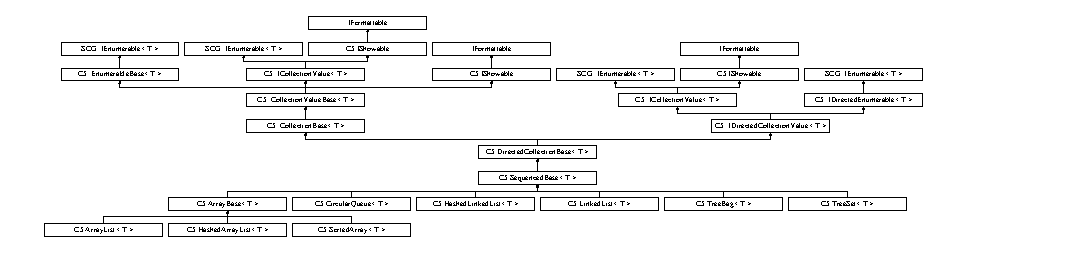
\includegraphics[height=2.957747cm]{class_c5_1_1_directed_collection_base}
\end{center}
\end{figure}
\subsection*{Public Member Functions}
\begin{DoxyCompactItemize}
\item 
abstract \hyperlink{interface_c5_1_1_i_directed_collection_value}{I\+Directed\+Collection\+Value}$<$ T $>$ \hyperlink{class_c5_1_1_directed_collection_base_a9a4c7d6571ff7d78ea5adcb0d8264ff1}{Backwards} ()
\item 
virtual bool \hyperlink{class_c5_1_1_directed_collection_base_a5dd3482ac69a6ef10092748c9953785b}{Find\+Last} (Func$<$ T, bool $>$ predicate, out T item)
\begin{DoxyCompactList}\small\item\em Check if there exists an item that satisfies a specific predicate in this collection and return the first one in enumeration order. \end{DoxyCompactList}\end{DoxyCompactItemize}
\subsection*{Protected Member Functions}
\begin{DoxyCompactItemize}
\item 
\hyperlink{class_c5_1_1_directed_collection_base_a59bb822bc2fdd8ba04cd778d958323d4}{Directed\+Collection\+Base} (S\+C\+G.\+I\+Equality\+Comparer$<$ T $>$ \hyperlink{class_c5_1_1_collection_base_a95e343400be0e8f3f8d6310f1aaf2cc6}{itemequality\+Comparer})
\end{DoxyCompactItemize}
\subsection*{Properties}
\begin{DoxyCompactItemize}
\item 
virtual \hyperlink{namespace_c5_aad282676794e49130eb8caed289395f8}{Enumeration\+Direction} \hyperlink{class_c5_1_1_directed_collection_base_a4e5eb8ce3c734029a03460ee73a571fc}{Direction}\hspace{0.3cm}{\ttfamily  \mbox{[}get\mbox{]}}
\end{DoxyCompactItemize}
\subsection*{Additional Inherited Members}


\subsection{Detailed Description}



\begin{DoxyTemplParams}{Template Parameters}
{\em T} & \\
\hline
\end{DoxyTemplParams}


\subsection{Constructor \& Destructor Documentation}
\hypertarget{class_c5_1_1_directed_collection_base_a59bb822bc2fdd8ba04cd778d958323d4}{}\index{C5\+::\+Directed\+Collection\+Base@{C5\+::\+Directed\+Collection\+Base}!Directed\+Collection\+Base@{Directed\+Collection\+Base}}
\index{Directed\+Collection\+Base@{Directed\+Collection\+Base}!C5\+::\+Directed\+Collection\+Base@{C5\+::\+Directed\+Collection\+Base}}
\subsubsection[{Directed\+Collection\+Base(\+S\+C\+G.\+I\+Equality\+Comparer$<$ T $>$ itemequality\+Comparer)}]{\setlength{\rightskip}{0pt plus 5cm}{\bf C5.\+Directed\+Collection\+Base}$<$ T $>$.{\bf Directed\+Collection\+Base} (
\begin{DoxyParamCaption}
\item[{S\+C\+G.\+I\+Equality\+Comparer$<$ T $>$}]{itemequality\+Comparer}
\end{DoxyParamCaption}
)\hspace{0.3cm}{\ttfamily [protected]}}\label{class_c5_1_1_directed_collection_base_a59bb822bc2fdd8ba04cd778d958323d4}





\begin{DoxyParams}{Parameters}
{\em itemequality\+Comparer} & \\
\hline
\end{DoxyParams}


\subsection{Member Function Documentation}
\hypertarget{class_c5_1_1_directed_collection_base_a9a4c7d6571ff7d78ea5adcb0d8264ff1}{}\index{C5\+::\+Directed\+Collection\+Base@{C5\+::\+Directed\+Collection\+Base}!Backwards@{Backwards}}
\index{Backwards@{Backwards}!C5\+::\+Directed\+Collection\+Base@{C5\+::\+Directed\+Collection\+Base}}
\subsubsection[{Backwards()}]{\setlength{\rightskip}{0pt plus 5cm}abstract {\bf I\+Directed\+Collection\+Value}$<$T$>$ {\bf C5.\+Directed\+Collection\+Base}$<$ T $>$.Backwards (
\begin{DoxyParamCaption}
{}
\end{DoxyParamCaption}
)\hspace{0.3cm}{\ttfamily [pure virtual]}}\label{class_c5_1_1_directed_collection_base_a9a4c7d6571ff7d78ea5adcb0d8264ff1}




\begin{DoxyReturn}{Returns}

\end{DoxyReturn}


Implements \hyperlink{interface_c5_1_1_i_directed_collection_value_ae5665ed396ea2801266c4b2bfb3dae41}{C5.\+I\+Directed\+Collection\+Value$<$ T $>$}.



Implemented in \hyperlink{class_c5_1_1_tree_bag_aa8d9bd7240bf759fc52c3a14b1f2e43a}{C5.\+Tree\+Bag$<$ T $>$}, \hyperlink{class_c5_1_1_tree_set_a27bc1208dc4fb8e7e1e3be048354ec7b}{C5.\+Tree\+Set$<$ T $>$}, \hyperlink{class_c5_1_1_hashed_linked_list_ad0fbbf15338c5aae4278a5e44f8d9c69}{C5.\+Hashed\+Linked\+List$<$ T $>$}, \hyperlink{class_c5_1_1_linked_list_aa96b744c5e2f0db894b8c9ed9606c240}{C5.\+Linked\+List$<$ T $>$}, \hyperlink{class_c5_1_1_array_base_a11fbdc5f71bb41de404f3bd91e3a92b3}{C5.\+Array\+Base$<$ T $>$}, and \hyperlink{class_c5_1_1_circular_queue_a9df19a0a07cd854a59df4d3f976cf169}{C5.\+Circular\+Queue$<$ T $>$}.

\hypertarget{class_c5_1_1_directed_collection_base_a5dd3482ac69a6ef10092748c9953785b}{}\index{C5\+::\+Directed\+Collection\+Base@{C5\+::\+Directed\+Collection\+Base}!Find\+Last@{Find\+Last}}
\index{Find\+Last@{Find\+Last}!C5\+::\+Directed\+Collection\+Base@{C5\+::\+Directed\+Collection\+Base}}
\subsubsection[{Find\+Last(\+Func$<$ T, bool $>$ predicate, out T item)}]{\setlength{\rightskip}{0pt plus 5cm}virtual bool {\bf C5.\+Directed\+Collection\+Base}$<$ T $>$.Find\+Last (
\begin{DoxyParamCaption}
\item[{Func$<$ T, bool $>$}]{predicate, }
\item[{out T}]{item}
\end{DoxyParamCaption}
)\hspace{0.3cm}{\ttfamily [virtual]}}\label{class_c5_1_1_directed_collection_base_a5dd3482ac69a6ef10092748c9953785b}


Check if there exists an item that satisfies a specific predicate in this collection and return the first one in enumeration order. 


\begin{DoxyParams}{Parameters}
{\em predicate} & A delegate (T\+:\+Func`2 with 
\begin{DoxyCode}
R == \textcolor{keywordtype}{bool}
\end{DoxyCode}
) defining the predicate\\
\hline
{\em item} & \\
\hline
\end{DoxyParams}
\begin{DoxyReturn}{Returns}
True is such an item exists
\end{DoxyReturn}


Implements \hyperlink{interface_c5_1_1_i_directed_collection_value_a93725b1f694e0d1cf5827e481ea467b7}{C5.\+I\+Directed\+Collection\+Value$<$ T $>$}.



\subsection{Property Documentation}
\hypertarget{class_c5_1_1_directed_collection_base_a4e5eb8ce3c734029a03460ee73a571fc}{}\index{C5\+::\+Directed\+Collection\+Base@{C5\+::\+Directed\+Collection\+Base}!Direction@{Direction}}
\index{Direction@{Direction}!C5\+::\+Directed\+Collection\+Base@{C5\+::\+Directed\+Collection\+Base}}
\subsubsection[{Direction}]{\setlength{\rightskip}{0pt plus 5cm}virtual {\bf Enumeration\+Direction} {\bf C5.\+Directed\+Collection\+Base}$<$ T $>$.Direction\hspace{0.3cm}{\ttfamily [get]}}\label{class_c5_1_1_directed_collection_base_a4e5eb8ce3c734029a03460ee73a571fc}




{\ttfamily Forwards} if same, else {\ttfamily Backwards} 

The enumeration direction relative to the original collection.

The documentation for this class was generated from the following file\+:\begin{DoxyCompactItemize}
\item 
C\+:/\+Users/rasmusl/\+Source/\+Repos/\+C5/\+C5/\hyperlink{_collections_8cs}{Collections.\+cs}\end{DoxyCompactItemize}

\hypertarget{class_c5_1_1_directed_collection_value_base}{}\section{C5.\+Directed\+Collection\+Value\+Base$<$ T $>$ Class Template Reference}
\label{class_c5_1_1_directed_collection_value_base}\index{C5.\+Directed\+Collection\+Value\+Base$<$ T $>$@{C5.\+Directed\+Collection\+Value\+Base$<$ T $>$}}


 


Inheritance diagram for C5.\+Directed\+Collection\+Value\+Base$<$ T $>$\+:\begin{figure}[H]
\begin{center}
\leavevmode
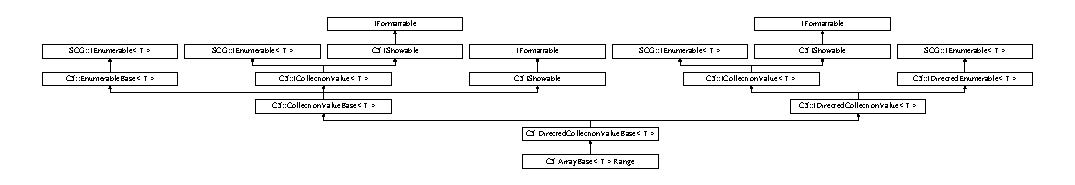
\includegraphics[height=2.033898cm]{class_c5_1_1_directed_collection_value_base}
\end{center}
\end{figure}
\subsection*{Public Member Functions}
\begin{DoxyCompactItemize}
\item 
abstract \hyperlink{interface_c5_1_1_i_directed_collection_value}{I\+Directed\+Collection\+Value}$<$ T $>$ \hyperlink{class_c5_1_1_directed_collection_value_base_a66d4222e083371d053e609efeecac740}{Backwards} ()
\item 
virtual bool \hyperlink{class_c5_1_1_directed_collection_value_base_af3d97f14823310f6afd1980d181a4f82}{Find\+Last} (Func$<$ T, bool $>$ predicate, out T item)
\begin{DoxyCompactList}\small\item\em Check if there exists an item that satisfies a specific predicate in this collection and return the first one in enumeration order. \end{DoxyCompactList}\end{DoxyCompactItemize}
\subsection*{Properties}
\begin{DoxyCompactItemize}
\item 
virtual \hyperlink{namespace_c5_aad282676794e49130eb8caed289395f8}{Enumeration\+Direction} \hyperlink{class_c5_1_1_directed_collection_value_base_acb1489d931bddb60b2d220b60e355021}{Direction}\hspace{0.3cm}{\ttfamily  \mbox{[}get\mbox{]}}
\end{DoxyCompactItemize}
\subsection*{Additional Inherited Members}


\subsection{Detailed Description}



\begin{DoxyTemplParams}{Template Parameters}
{\em T} & \\
\hline
\end{DoxyTemplParams}


\subsection{Member Function Documentation}
\hypertarget{class_c5_1_1_directed_collection_value_base_a66d4222e083371d053e609efeecac740}{}\index{C5\+::\+Directed\+Collection\+Value\+Base@{C5\+::\+Directed\+Collection\+Value\+Base}!Backwards@{Backwards}}
\index{Backwards@{Backwards}!C5\+::\+Directed\+Collection\+Value\+Base@{C5\+::\+Directed\+Collection\+Value\+Base}}
\subsubsection[{Backwards()}]{\setlength{\rightskip}{0pt plus 5cm}abstract {\bf I\+Directed\+Collection\+Value}$<$T$>$ {\bf C5.\+Directed\+Collection\+Value\+Base}$<$ T $>$.Backwards (
\begin{DoxyParamCaption}
{}
\end{DoxyParamCaption}
)\hspace{0.3cm}{\ttfamily [pure virtual]}}\label{class_c5_1_1_directed_collection_value_base_a66d4222e083371d053e609efeecac740}




\begin{DoxyReturn}{Returns}

\end{DoxyReturn}


Implements \hyperlink{interface_c5_1_1_i_directed_collection_value_ae5665ed396ea2801266c4b2bfb3dae41}{C5.\+I\+Directed\+Collection\+Value$<$ T $>$}.



Implemented in \hyperlink{class_c5_1_1_array_base_1_1_range_a296cf1453eb618368fdc14f7abc4f4c2}{C5.\+Array\+Base$<$ T $>$.\+Range}, and \hyperlink{class_c5_1_1_mapped_directed_collection_value_a8eaadbb8ae6d18393c504361daec1c8c}{C5.\+Mapped\+Directed\+Collection\+Value$<$ T, V $>$}.

\hypertarget{class_c5_1_1_directed_collection_value_base_af3d97f14823310f6afd1980d181a4f82}{}\index{C5\+::\+Directed\+Collection\+Value\+Base@{C5\+::\+Directed\+Collection\+Value\+Base}!Find\+Last@{Find\+Last}}
\index{Find\+Last@{Find\+Last}!C5\+::\+Directed\+Collection\+Value\+Base@{C5\+::\+Directed\+Collection\+Value\+Base}}
\subsubsection[{Find\+Last(\+Func$<$ T, bool $>$ predicate, out T item)}]{\setlength{\rightskip}{0pt plus 5cm}virtual bool {\bf C5.\+Directed\+Collection\+Value\+Base}$<$ T $>$.Find\+Last (
\begin{DoxyParamCaption}
\item[{Func$<$ T, bool $>$}]{predicate, }
\item[{out T}]{item}
\end{DoxyParamCaption}
)\hspace{0.3cm}{\ttfamily [virtual]}}\label{class_c5_1_1_directed_collection_value_base_af3d97f14823310f6afd1980d181a4f82}


Check if there exists an item that satisfies a specific predicate in this collection and return the first one in enumeration order. 


\begin{DoxyParams}{Parameters}
{\em predicate} & A delegate (T\+:\+Func`2 with 
\begin{DoxyCode}
R == \textcolor{keywordtype}{bool}
\end{DoxyCode}
) defining the predicate\\
\hline
{\em item} & \\
\hline
\end{DoxyParams}
\begin{DoxyReturn}{Returns}
True is such an item exists
\end{DoxyReturn}


Implements \hyperlink{interface_c5_1_1_i_directed_collection_value_a93725b1f694e0d1cf5827e481ea467b7}{C5.\+I\+Directed\+Collection\+Value$<$ T $>$}.



\subsection{Property Documentation}
\hypertarget{class_c5_1_1_directed_collection_value_base_acb1489d931bddb60b2d220b60e355021}{}\index{C5\+::\+Directed\+Collection\+Value\+Base@{C5\+::\+Directed\+Collection\+Value\+Base}!Direction@{Direction}}
\index{Direction@{Direction}!C5\+::\+Directed\+Collection\+Value\+Base@{C5\+::\+Directed\+Collection\+Value\+Base}}
\subsubsection[{Direction}]{\setlength{\rightskip}{0pt plus 5cm}virtual {\bf Enumeration\+Direction} {\bf C5.\+Directed\+Collection\+Value\+Base}$<$ T $>$.Direction\hspace{0.3cm}{\ttfamily [get]}}\label{class_c5_1_1_directed_collection_value_base_acb1489d931bddb60b2d220b60e355021}




{\ttfamily Forwards} if same, else {\ttfamily Backwards} 

The enumeration direction relative to the original collection.

The documentation for this class was generated from the following file\+:\begin{DoxyCompactItemize}
\item 
C\+:/\+Users/rasmusl/\+Source/\+Repos/\+C5/\+C5/\hyperlink{_collections_8cs}{Collections.\+cs}\end{DoxyCompactItemize}

\hypertarget{class_c5_1_1_drop_multiplicity}{}\section{C5.\+Drop\+Multiplicity$<$ K $>$ Class Template Reference}
\label{class_c5_1_1_drop_multiplicity}\index{C5.\+Drop\+Multiplicity$<$ K $>$@{C5.\+Drop\+Multiplicity$<$ K $>$}}
Inheritance diagram for C5.\+Drop\+Multiplicity$<$ K $>$\+:\begin{figure}[H]
\begin{center}
\leavevmode
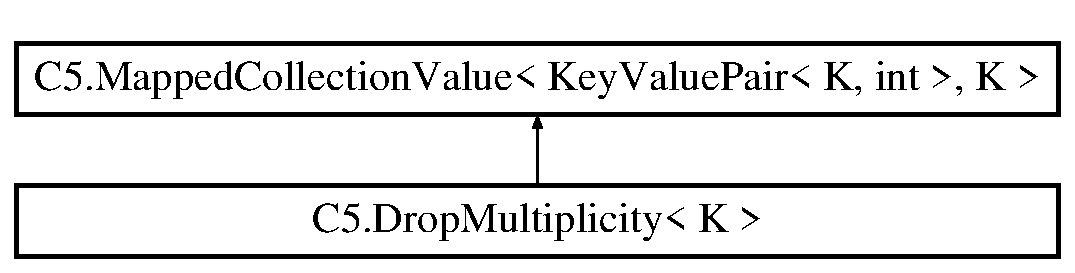
\includegraphics[height=2.000000cm]{class_c5_1_1_drop_multiplicity}
\end{center}
\end{figure}
\subsection*{Public Member Functions}
\begin{DoxyCompactItemize}
\item 
\hyperlink{class_c5_1_1_drop_multiplicity_a0e89ccf6e0c868e6cbfd7858563c3ca2}{Drop\+Multiplicity} (\hyperlink{interface_c5_1_1_i_collection_value}{I\+Collection\+Value}$<$ \hyperlink{struct_c5_1_1_key_value_pair}{Key\+Value\+Pair}$<$ K, int $>$$>$ coll)
\item 
override K \hyperlink{class_c5_1_1_drop_multiplicity_a95814913c22366178d5dd862990e4671}{Map} (\hyperlink{struct_c5_1_1_key_value_pair}{Key\+Value\+Pair}$<$ K, int $>$ kvp)
\end{DoxyCompactItemize}
\subsection*{Additional Inherited Members}


\subsection{Constructor \& Destructor Documentation}
\hypertarget{class_c5_1_1_drop_multiplicity_a0e89ccf6e0c868e6cbfd7858563c3ca2}{}\index{C5\+::\+Drop\+Multiplicity@{C5\+::\+Drop\+Multiplicity}!Drop\+Multiplicity@{Drop\+Multiplicity}}
\index{Drop\+Multiplicity@{Drop\+Multiplicity}!C5\+::\+Drop\+Multiplicity@{C5\+::\+Drop\+Multiplicity}}
\subsubsection[{Drop\+Multiplicity(\+I\+Collection\+Value$<$ Key\+Value\+Pair$<$ K, int $>$$>$ coll)}]{\setlength{\rightskip}{0pt plus 5cm}{\bf C5.\+Drop\+Multiplicity}$<$ K $>$.{\bf Drop\+Multiplicity} (
\begin{DoxyParamCaption}
\item[{{\bf I\+Collection\+Value}$<$ {\bf Key\+Value\+Pair}$<$ K, int $>$$>$}]{coll}
\end{DoxyParamCaption}
)}\label{class_c5_1_1_drop_multiplicity_a0e89ccf6e0c868e6cbfd7858563c3ca2}


\subsection{Member Function Documentation}
\hypertarget{class_c5_1_1_drop_multiplicity_a95814913c22366178d5dd862990e4671}{}\index{C5\+::\+Drop\+Multiplicity@{C5\+::\+Drop\+Multiplicity}!Map@{Map}}
\index{Map@{Map}!C5\+::\+Drop\+Multiplicity@{C5\+::\+Drop\+Multiplicity}}
\subsubsection[{Map(\+Key\+Value\+Pair$<$ K, int $>$ kvp)}]{\setlength{\rightskip}{0pt plus 5cm}override K {\bf C5.\+Drop\+Multiplicity}$<$ K $>$.Map (
\begin{DoxyParamCaption}
\item[{{\bf Key\+Value\+Pair}$<$ K, int $>$}]{kvp}
\end{DoxyParamCaption}
)}\label{class_c5_1_1_drop_multiplicity_a95814913c22366178d5dd862990e4671}


The documentation for this class was generated from the following file\+:\begin{DoxyCompactItemize}
\item 
C\+:/\+Users/rasmusl/\+Source/\+Repos/\+C5/\+C5/\hyperlink{_mapped_enumerators_8cs}{Mapped\+Enumerators.\+cs}\end{DoxyCompactItemize}

\hypertarget{class_c5_1_1_duplicate_not_allowed_exception}{}\section{C5.\+Duplicate\+Not\+Allowed\+Exception Class Reference}
\label{class_c5_1_1_duplicate_not_allowed_exception}\index{C5.\+Duplicate\+Not\+Allowed\+Exception@{C5.\+Duplicate\+Not\+Allowed\+Exception}}


An exception thrown when an operation attempts to create a duplicate in a collection with set semantics (P\+:\+C5.\+I\+Extensible`1.\+Allows\+Duplicates is false) or attempts to create a duplicate key in a dictionary.  


Inheritance diagram for C5.\+Duplicate\+Not\+Allowed\+Exception\+:\begin{figure}[H]
\begin{center}
\leavevmode
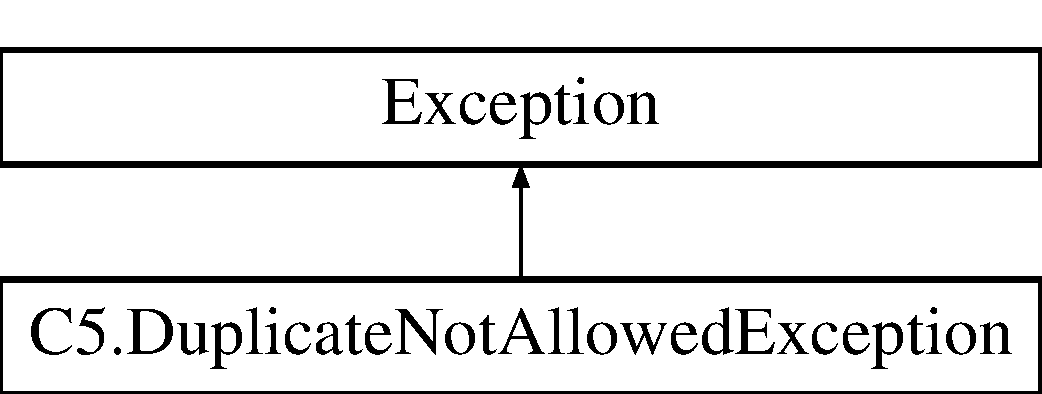
\includegraphics[height=2.000000cm]{class_c5_1_1_duplicate_not_allowed_exception}
\end{center}
\end{figure}
\subsection*{Public Member Functions}
\begin{DoxyCompactItemize}
\item 
\hyperlink{class_c5_1_1_duplicate_not_allowed_exception_a57f60c225b3ef8850b3c56e1f3089e60}{Duplicate\+Not\+Allowed\+Exception} ()
\begin{DoxyCompactList}\small\item\em Create a simple exception with no further explanation. \end{DoxyCompactList}\item 
\hyperlink{class_c5_1_1_duplicate_not_allowed_exception_a674b91b55cfad4db40a204efecfa1449}{Duplicate\+Not\+Allowed\+Exception} (string message)
\begin{DoxyCompactList}\small\item\em Create the exception with an explanation of the reason. \end{DoxyCompactList}\end{DoxyCompactItemize}


\subsection{Detailed Description}
An exception thrown when an operation attempts to create a duplicate in a collection with set semantics (P\+:\+C5.\+I\+Extensible`1.\+Allows\+Duplicates is false) or attempts to create a duplicate key in a dictionary. 

With collections this can only happen with Insert operations on lists, since the Add operations will not try to create duplictes and either ignore the failure or report it in a bool return value. 

With dictionaries this can happen with the M\+:\+C5.\+I\+Dictionary`2.\+Add(`0,`1) metod.

\subsection{Constructor \& Destructor Documentation}
\hypertarget{class_c5_1_1_duplicate_not_allowed_exception_a57f60c225b3ef8850b3c56e1f3089e60}{}\index{C5\+::\+Duplicate\+Not\+Allowed\+Exception@{C5\+::\+Duplicate\+Not\+Allowed\+Exception}!Duplicate\+Not\+Allowed\+Exception@{Duplicate\+Not\+Allowed\+Exception}}
\index{Duplicate\+Not\+Allowed\+Exception@{Duplicate\+Not\+Allowed\+Exception}!C5\+::\+Duplicate\+Not\+Allowed\+Exception@{C5\+::\+Duplicate\+Not\+Allowed\+Exception}}
\subsubsection[{Duplicate\+Not\+Allowed\+Exception()}]{\setlength{\rightskip}{0pt plus 5cm}C5.\+Duplicate\+Not\+Allowed\+Exception.\+Duplicate\+Not\+Allowed\+Exception (
\begin{DoxyParamCaption}
{}
\end{DoxyParamCaption}
)}\label{class_c5_1_1_duplicate_not_allowed_exception_a57f60c225b3ef8850b3c56e1f3089e60}


Create a simple exception with no further explanation. 

\hypertarget{class_c5_1_1_duplicate_not_allowed_exception_a674b91b55cfad4db40a204efecfa1449}{}\index{C5\+::\+Duplicate\+Not\+Allowed\+Exception@{C5\+::\+Duplicate\+Not\+Allowed\+Exception}!Duplicate\+Not\+Allowed\+Exception@{Duplicate\+Not\+Allowed\+Exception}}
\index{Duplicate\+Not\+Allowed\+Exception@{Duplicate\+Not\+Allowed\+Exception}!C5\+::\+Duplicate\+Not\+Allowed\+Exception@{C5\+::\+Duplicate\+Not\+Allowed\+Exception}}
\subsubsection[{Duplicate\+Not\+Allowed\+Exception(string message)}]{\setlength{\rightskip}{0pt plus 5cm}C5.\+Duplicate\+Not\+Allowed\+Exception.\+Duplicate\+Not\+Allowed\+Exception (
\begin{DoxyParamCaption}
\item[{string}]{message}
\end{DoxyParamCaption}
)}\label{class_c5_1_1_duplicate_not_allowed_exception_a674b91b55cfad4db40a204efecfa1449}


Create the exception with an explanation of the reason. 


\begin{DoxyParams}{Parameters}
{\em message} & \\
\hline
\end{DoxyParams}


The documentation for this class was generated from the following file\+:\begin{DoxyCompactItemize}
\item 
C\+:/\+Users/rasmusl/\+Source/\+Repos/\+C5/\+C5/\hyperlink{_exceptions_8cs}{Exceptions.\+cs}\end{DoxyCompactItemize}

\hypertarget{class_c5_1_1_enumerable_base}{}\section{C5.\+Enumerable\+Base$<$ T $>$ Class Template Reference}
\label{class_c5_1_1_enumerable_base}\index{C5.\+Enumerable\+Base$<$ T $>$@{C5.\+Enumerable\+Base$<$ T $>$}}


A base class for implementing an I\+Enumerable$<$T$>$  


Inheritance diagram for C5.\+Enumerable\+Base$<$ T $>$\+:\begin{figure}[H]
\begin{center}
\leavevmode
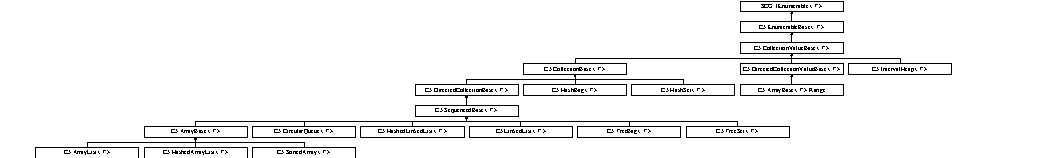
\includegraphics[height=2.109228cm]{class_c5_1_1_enumerable_base}
\end{center}
\end{figure}
\subsection*{Public Member Functions}
\begin{DoxyCompactItemize}
\item 
abstract S\+C\+G.\+I\+Enumerator$<$ T $>$ \hyperlink{class_c5_1_1_enumerable_base_ad8893620ea9cc4e7d41c17d26769d237}{Get\+Enumerator} ()
\begin{DoxyCompactList}\small\item\em Create an enumerator for this collection. \end{DoxyCompactList}\end{DoxyCompactItemize}
\subsection*{Static Protected Member Functions}
\begin{DoxyCompactItemize}
\item 
static int \hyperlink{class_c5_1_1_enumerable_base_ad696d9c2a4370aa2e7611961bf3f815a}{count\+Items} (S\+C\+G.\+I\+Enumerable$<$ T $>$ items)
\begin{DoxyCompactList}\small\item\em Count the number of items in an enumerable by enumeration \end{DoxyCompactList}\end{DoxyCompactItemize}


\subsection{Detailed Description}
A base class for implementing an I\+Enumerable$<$T$>$ 



\subsection{Member Function Documentation}
\hypertarget{class_c5_1_1_enumerable_base_ad696d9c2a4370aa2e7611961bf3f815a}{}\index{C5\+::\+Enumerable\+Base@{C5\+::\+Enumerable\+Base}!count\+Items@{count\+Items}}
\index{count\+Items@{count\+Items}!C5\+::\+Enumerable\+Base@{C5\+::\+Enumerable\+Base}}
\subsubsection[{count\+Items(\+S\+C\+G.\+I\+Enumerable$<$ T $>$ items)}]{\setlength{\rightskip}{0pt plus 5cm}static int {\bf C5.\+Enumerable\+Base}$<$ T $>$.count\+Items (
\begin{DoxyParamCaption}
\item[{S\+C\+G.\+I\+Enumerable$<$ T $>$}]{items}
\end{DoxyParamCaption}
)\hspace{0.3cm}{\ttfamily [static]}, {\ttfamily [protected]}}\label{class_c5_1_1_enumerable_base_ad696d9c2a4370aa2e7611961bf3f815a}


Count the number of items in an enumerable by enumeration 


\begin{DoxyParams}{Parameters}
{\em items} & The enumerable to count\\
\hline
\end{DoxyParams}
\begin{DoxyReturn}{Returns}
The size of the enumerable
\end{DoxyReturn}
\hypertarget{class_c5_1_1_enumerable_base_ad8893620ea9cc4e7d41c17d26769d237}{}\index{C5\+::\+Enumerable\+Base@{C5\+::\+Enumerable\+Base}!Get\+Enumerator@{Get\+Enumerator}}
\index{Get\+Enumerator@{Get\+Enumerator}!C5\+::\+Enumerable\+Base@{C5\+::\+Enumerable\+Base}}
\subsubsection[{Get\+Enumerator()}]{\setlength{\rightskip}{0pt plus 5cm}abstract S\+C\+G.\+I\+Enumerator$<$T$>$ {\bf C5.\+Enumerable\+Base}$<$ T $>$.Get\+Enumerator (
\begin{DoxyParamCaption}
{}
\end{DoxyParamCaption}
)\hspace{0.3cm}{\ttfamily [pure virtual]}}\label{class_c5_1_1_enumerable_base_ad8893620ea9cc4e7d41c17d26769d237}


Create an enumerator for this collection. 

\begin{DoxyReturn}{Returns}
The enumerator
\end{DoxyReturn}


Implemented in \hyperlink{class_c5_1_1_hashed_linked_list_ae8f40668f13afb6cb05501446a3bcc4e}{C5.\+Hashed\+Linked\+List$<$ T $>$}, \hyperlink{class_c5_1_1_linked_list_ab23965434fba5e39a15eb4c0eb3c4901}{C5.\+Linked\+List$<$ T $>$}, \hyperlink{class_c5_1_1_hashed_array_list_a0ce81bee1c45ccbc3105698a4f4692a8}{C5.\+Hashed\+Array\+List$<$ T $>$}, \hyperlink{class_c5_1_1_array_list_ae6c2dc2f2aa8c9952d3267a37e9de01a}{C5.\+Array\+List$<$ T $>$}, \hyperlink{class_c5_1_1_array_base_1_1_range_af6396c46d77d98185e8587c024dd9316}{C5.\+Array\+Base$<$ T $>$.\+Range}, \hyperlink{class_c5_1_1_array_base_a84a54c5fa039db32e27ca45c6b0cea85}{C5.\+Array\+Base$<$ T $>$}, \hyperlink{class_c5_1_1_sequenced_base_a07d117175b630fd7f87f6e61b05259dc}{C5.\+Sequenced\+Base$<$ T $>$}, \hyperlink{class_c5_1_1_collection_base_a3b4b98e2606afecb948019412c4c2533}{C5.\+Collection\+Base$<$ T $>$}, \hyperlink{class_c5_1_1_hash_set_a4c404a22695abc0f6b47bf74d3d34034}{C5.\+Hash\+Set$<$ T $>$}, \hyperlink{class_c5_1_1_hash_bag_a621d77b2f8a7c3a826aace4be1d809b2}{C5.\+Hash\+Bag$<$ T $>$}, \hyperlink{class_c5_1_1_tree_bag_a2c00797c0e29dd52efa05f219b4c9c7e}{C5.\+Tree\+Bag$<$ T $>$}, \hyperlink{class_c5_1_1_tree_set_af9dd4aece1415276e1ede1ded6904179}{C5.\+Tree\+Set$<$ T $>$}, \hyperlink{class_c5_1_1_collection_value_base_a0e8b891322ed9987a18f1a1ac87d2d4f}{C5.\+Collection\+Value\+Base$<$ T $>$}, \hyperlink{class_c5_1_1_interval_heap_a09556ba66252a46d94456587bc877561}{C5.\+Interval\+Heap$<$ T $>$}, \hyperlink{class_c5_1_1_circular_queue_ae1ab5e745ced280db9b9a175a66dc5b4}{C5.\+Circular\+Queue$<$ T $>$}, and \hyperlink{class_c5_1_1_mapped_directed_enumerable_a20cbeb4a43b678a5d3d4f6d0c3e5497b}{C5.\+Mapped\+Directed\+Enumerable$<$ T, V $>$}.



The documentation for this class was generated from the following file\+:\begin{DoxyCompactItemize}
\item 
C\+:/\+Users/rasmusl/\+Source/\+Repos/\+C5/\+C5/\hyperlink{_collections_8cs}{Collections.\+cs}\end{DoxyCompactItemize}

\hypertarget{class_c5_1_1_fixed_size_collection_exception}{}\section{C5.\+Fixed\+Size\+Collection\+Exception Class Reference}
\label{class_c5_1_1_fixed_size_collection_exception}\index{C5.\+Fixed\+Size\+Collection\+Exception@{C5.\+Fixed\+Size\+Collection\+Exception}}


 


Inheritance diagram for C5.\+Fixed\+Size\+Collection\+Exception\+:\begin{figure}[H]
\begin{center}
\leavevmode
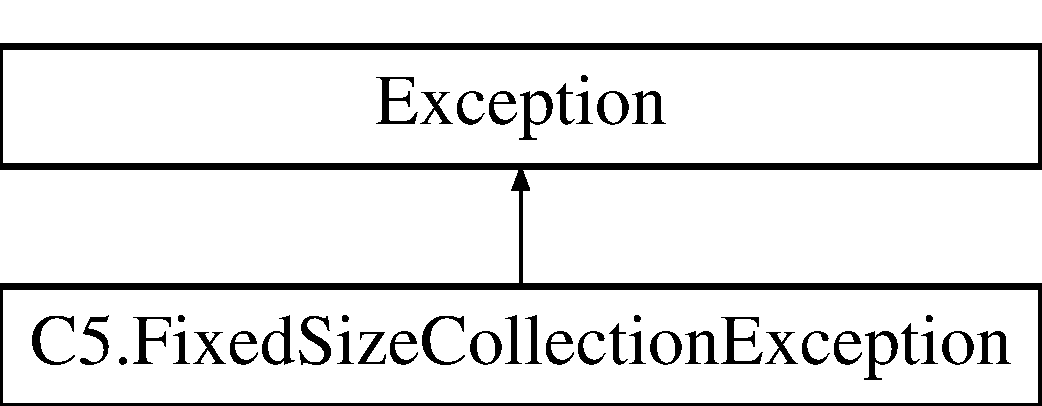
\includegraphics[height=2.000000cm]{class_c5_1_1_fixed_size_collection_exception}
\end{center}
\end{figure}
\subsection*{Public Member Functions}
\begin{DoxyCompactItemize}
\item 
\hyperlink{class_c5_1_1_fixed_size_collection_exception_a7d03d1dfcd8346fd83a5fe1a585632d9}{Fixed\+Size\+Collection\+Exception} ()
\begin{DoxyCompactList}\small\item\em Create a simple exception with no further explanation. \end{DoxyCompactList}\item 
\hyperlink{class_c5_1_1_fixed_size_collection_exception_add85f9d2208c64dd9bc74a6c1a31733b}{Fixed\+Size\+Collection\+Exception} (string message)
\begin{DoxyCompactList}\small\item\em Create the exception with an explanation of the reason. \end{DoxyCompactList}\end{DoxyCompactItemize}


\subsection{Detailed Description}




\subsection{Constructor \& Destructor Documentation}
\hypertarget{class_c5_1_1_fixed_size_collection_exception_a7d03d1dfcd8346fd83a5fe1a585632d9}{}\index{C5\+::\+Fixed\+Size\+Collection\+Exception@{C5\+::\+Fixed\+Size\+Collection\+Exception}!Fixed\+Size\+Collection\+Exception@{Fixed\+Size\+Collection\+Exception}}
\index{Fixed\+Size\+Collection\+Exception@{Fixed\+Size\+Collection\+Exception}!C5\+::\+Fixed\+Size\+Collection\+Exception@{C5\+::\+Fixed\+Size\+Collection\+Exception}}
\subsubsection[{Fixed\+Size\+Collection\+Exception()}]{\setlength{\rightskip}{0pt plus 5cm}C5.\+Fixed\+Size\+Collection\+Exception.\+Fixed\+Size\+Collection\+Exception (
\begin{DoxyParamCaption}
{}
\end{DoxyParamCaption}
)}\label{class_c5_1_1_fixed_size_collection_exception_a7d03d1dfcd8346fd83a5fe1a585632d9}


Create a simple exception with no further explanation. 

\hypertarget{class_c5_1_1_fixed_size_collection_exception_add85f9d2208c64dd9bc74a6c1a31733b}{}\index{C5\+::\+Fixed\+Size\+Collection\+Exception@{C5\+::\+Fixed\+Size\+Collection\+Exception}!Fixed\+Size\+Collection\+Exception@{Fixed\+Size\+Collection\+Exception}}
\index{Fixed\+Size\+Collection\+Exception@{Fixed\+Size\+Collection\+Exception}!C5\+::\+Fixed\+Size\+Collection\+Exception@{C5\+::\+Fixed\+Size\+Collection\+Exception}}
\subsubsection[{Fixed\+Size\+Collection\+Exception(string message)}]{\setlength{\rightskip}{0pt plus 5cm}C5.\+Fixed\+Size\+Collection\+Exception.\+Fixed\+Size\+Collection\+Exception (
\begin{DoxyParamCaption}
\item[{string}]{message}
\end{DoxyParamCaption}
)}\label{class_c5_1_1_fixed_size_collection_exception_add85f9d2208c64dd9bc74a6c1a31733b}


Create the exception with an explanation of the reason. 


\begin{DoxyParams}{Parameters}
{\em message} & \\
\hline
\end{DoxyParams}


The documentation for this class was generated from the following file\+:\begin{DoxyCompactItemize}
\item 
C\+:/\+Users/rasmusl/\+Source/\+Repos/\+C5/\+C5/\hyperlink{_exceptions_8cs}{Exceptions.\+cs}\end{DoxyCompactItemize}

\hypertarget{class_c5_1_1_guarded_collection}{}\section{C5.\+Guarded\+Collection$<$ T $>$ Class Template Reference}
\label{class_c5_1_1_guarded_collection}\index{C5.\+Guarded\+Collection$<$ T $>$@{C5.\+Guarded\+Collection$<$ T $>$}}


A read-\/only wrapper for an T\+:\+C5.\+I\+Collection`1,  


Inheritance diagram for C5.\+Guarded\+Collection$<$ T $>$\+:\begin{figure}[H]
\begin{center}
\leavevmode
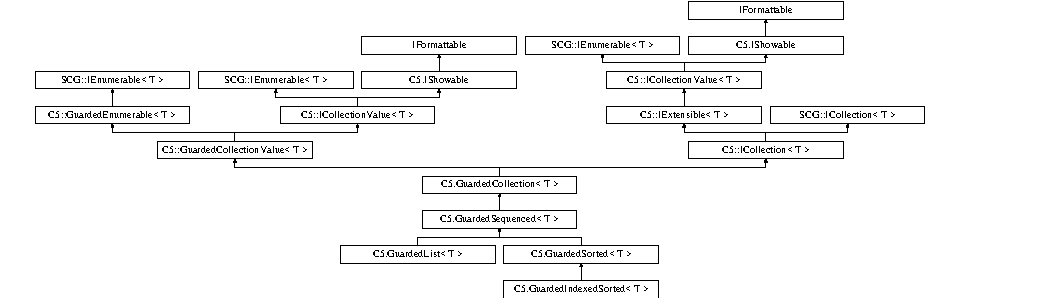
\includegraphics[height=3.981043cm]{class_c5_1_1_guarded_collection}
\end{center}
\end{figure}
\subsection*{Public Member Functions}
\begin{DoxyCompactItemize}
\item 
\hyperlink{class_c5_1_1_guarded_collection_af940d400b312c53974a6760b141a0678}{Guarded\+Collection} (\hyperlink{interface_c5_1_1_i_collection}{I\+Collection}$<$ T $>$ collection)
\begin{DoxyCompactList}\small\item\em Wrap an \hyperlink{interface_c5_1_1_i_collection}{I\+Collection}$<$T$>$ in a read-\/only wrapper \end{DoxyCompactList}\item 
virtual int \hyperlink{class_c5_1_1_guarded_collection_a993f9bfefdd11d4bf8f776215db02c31}{Get\+Unsequenced\+Hash\+Code} ()
\item 
virtual bool \hyperlink{class_c5_1_1_guarded_collection_ada1904ad7956b9e72606e2f9082642d7}{Unsequenced\+Equals} (\hyperlink{interface_c5_1_1_i_collection}{I\+Collection}$<$ T $>$ that)
\item 
virtual bool \hyperlink{class_c5_1_1_guarded_collection_a1ffdf15a3e9daa80137e53fcd642770e}{Contains} (T item)
\begin{DoxyCompactList}\small\item\em Check if an item is in the wrapped collection \end{DoxyCompactList}\item 
virtual int \hyperlink{class_c5_1_1_guarded_collection_ae5bfa7d92d0ebe7d185f04f8836685c7}{Contains\+Count} (T item)
\begin{DoxyCompactList}\small\item\em Count the number of times an item appears in the wrapped collection \end{DoxyCompactList}\item 
virtual \hyperlink{interface_c5_1_1_i_collection_value}{I\+Collection\+Value}$<$ T $>$ \hyperlink{class_c5_1_1_guarded_collection_a2a600a8efdfc23bcf87ae310cfbe8120}{Unique\+Items} ()
\item 
virtual \hyperlink{interface_c5_1_1_i_collection_value}{I\+Collection\+Value}$<$ \hyperlink{struct_c5_1_1_key_value_pair}{Key\+Value\+Pair}$<$ T, int $>$ $>$ \hyperlink{class_c5_1_1_guarded_collection_ad400f5862b15a3a0c59a4cb7d347f926}{Item\+Multiplicities} ()
\item 
virtual bool \hyperlink{class_c5_1_1_guarded_collection_a57f6d96d3787483e45837b2700d9459b}{Contains\+All} (S\+C\+G.\+I\+Enumerable$<$ T $>$ items)
\begin{DoxyCompactList}\small\item\em Check if all items in the argument is in the wrapped collection \end{DoxyCompactList}\item 
virtual bool \hyperlink{class_c5_1_1_guarded_collection_ab447aa674e79536b0c92f7010101ce89}{Find} (ref T item)
\begin{DoxyCompactList}\small\item\em Search for an item in the wrapped collection \end{DoxyCompactList}\item 
virtual bool \hyperlink{class_c5_1_1_guarded_collection_a06f9fdffc49fe7e5d618366b749fe8be}{Find\+Or\+Add} (ref T item)
\item 
virtual bool \hyperlink{class_c5_1_1_guarded_collection_a352f685be2677d2df5225e50aecb21cf}{Update} (T item)
\item 
virtual bool \hyperlink{class_c5_1_1_guarded_collection_a71d59b799800f0271a6a36a6fdea2f53}{Update} (T item, out T olditem)
\item 
virtual bool \hyperlink{class_c5_1_1_guarded_collection_a8cf85ddaca2e6fc07d6c4461feb9981f}{Update\+Or\+Add} (T item)
\item 
virtual bool \hyperlink{class_c5_1_1_guarded_collection_a0ff18d72c676480a225f9d3e3dacfcd0}{Update\+Or\+Add} (T item, out T olditem)
\item 
virtual bool \hyperlink{class_c5_1_1_guarded_collection_a5228eac1c6eb5341b2ab20a3095fa066}{Remove} (T item)
\item 
virtual bool \hyperlink{class_c5_1_1_guarded_collection_afa3304903fb8b724e52bb6cc4f12e6a9}{Remove} (T item, out T removeditem)
\item 
virtual void \hyperlink{class_c5_1_1_guarded_collection_a912c6184ee4b074c3981f9dde491a94b}{Remove\+All\+Copies} (T item)
\item 
virtual void \hyperlink{class_c5_1_1_guarded_collection_ab5e36593deb380b90bb35f7a283e48fc}{Remove\+All} (S\+C\+G.\+I\+Enumerable$<$ T $>$ items)
\item 
virtual void \hyperlink{class_c5_1_1_guarded_collection_ae26dd6085a063dd2b86d37b030b87750}{Clear} ()
\item 
virtual void \hyperlink{class_c5_1_1_guarded_collection_addd89e0bb9db15b64f24d64b7720761d}{Retain\+All} (S\+C\+G.\+I\+Enumerable$<$ T $>$ items)
\item 
virtual bool \hyperlink{class_c5_1_1_guarded_collection_adff17cbe1d82defc187161f1038225fe}{Check} ()
\begin{DoxyCompactList}\small\item\em Check wrapped collection for internal consistency \end{DoxyCompactList}\item 
virtual bool \hyperlink{class_c5_1_1_guarded_collection_aa7fe8941b3b05d9e8622b830852cf12d}{Add} (T item)
\item 
virtual void \hyperlink{class_c5_1_1_guarded_collection_ac93971d6ad817a2797bf01dbb1d30d12}{Add\+All} (S\+C\+G.\+I\+Enumerable$<$ T $>$ items)
\end{DoxyCompactItemize}
\subsection*{Properties}
\begin{DoxyCompactItemize}
\item 
virtual bool \hyperlink{class_c5_1_1_guarded_collection_ae7060bcf53641981bda57c113cd2e017}{Is\+Read\+Only}\hspace{0.3cm}{\ttfamily  \mbox{[}get\mbox{]}}
\begin{DoxyCompactList}\small\item\em (This is a read-\/only wrapper) \end{DoxyCompactList}\item 
virtual \hyperlink{namespace_c5_a615ba88dcdaa8d5a3c5f833a73d7fad6}{Speed} \hyperlink{class_c5_1_1_guarded_collection_a4c6ae95c3e5066e8f657546606deefaf}{Contains\+Speed}\hspace{0.3cm}{\ttfamily  \mbox{[}get\mbox{]}}
\item 
virtual bool \hyperlink{class_c5_1_1_guarded_collection_ac879f9062572ce67048d438409b1f8a9}{Allows\+Duplicates}\hspace{0.3cm}{\ttfamily  \mbox{[}get\mbox{]}}
\item 
virtual S\+C\+G.\+I\+Equality\+Comparer$<$ T $>$ \hyperlink{class_c5_1_1_guarded_collection_a71c7b8ae4fa03c0100428c7bd76db71e}{Equality\+Comparer}\hspace{0.3cm}{\ttfamily  \mbox{[}get\mbox{]}}
\item 
virtual bool \hyperlink{class_c5_1_1_guarded_collection_a02b79c68161065d8e2c6ddc89f004aea}{Duplicates\+By\+Counting}\hspace{0.3cm}{\ttfamily  \mbox{[}get\mbox{]}}
\begin{DoxyCompactList}\small\item\em By convention this is true for any collection with set semantics. \end{DoxyCompactList}\item 
override bool \hyperlink{class_c5_1_1_guarded_collection_a9a2e5fbcc49ab5a00eb4d2b929a03761}{Is\+Empty}\hspace{0.3cm}{\ttfamily  \mbox{[}get\mbox{]}}
\end{DoxyCompactItemize}
\subsection*{Additional Inherited Members}


\subsection{Detailed Description}
A read-\/only wrapper for an T\+:\+C5.\+I\+Collection`1, 

{\itshape Suitable for wrapping hash tables, T\+:\+C5.\+Hash\+Set`1 and T\+:\+C5.\+Hash\+Bag`1 }

\subsection{Constructor \& Destructor Documentation}
\hypertarget{class_c5_1_1_guarded_collection_af940d400b312c53974a6760b141a0678}{}\index{C5\+::\+Guarded\+Collection@{C5\+::\+Guarded\+Collection}!Guarded\+Collection@{Guarded\+Collection}}
\index{Guarded\+Collection@{Guarded\+Collection}!C5\+::\+Guarded\+Collection@{C5\+::\+Guarded\+Collection}}
\subsubsection[{Guarded\+Collection(\+I\+Collection$<$ T $>$ collection)}]{\setlength{\rightskip}{0pt plus 5cm}{\bf C5.\+Guarded\+Collection}$<$ T $>$.{\bf Guarded\+Collection} (
\begin{DoxyParamCaption}
\item[{{\bf I\+Collection}$<$ T $>$}]{collection}
\end{DoxyParamCaption}
)}\label{class_c5_1_1_guarded_collection_af940d400b312c53974a6760b141a0678}


Wrap an \hyperlink{interface_c5_1_1_i_collection}{I\+Collection}$<$T$>$ in a read-\/only wrapper 


\begin{DoxyParams}{Parameters}
{\em collection} & the collection to wrap\\
\hline
\end{DoxyParams}


\subsection{Member Function Documentation}
\hypertarget{class_c5_1_1_guarded_collection_aa7fe8941b3b05d9e8622b830852cf12d}{}\index{C5\+::\+Guarded\+Collection@{C5\+::\+Guarded\+Collection}!Add@{Add}}
\index{Add@{Add}!C5\+::\+Guarded\+Collection@{C5\+::\+Guarded\+Collection}}
\subsubsection[{Add(\+T item)}]{\setlength{\rightskip}{0pt plus 5cm}virtual bool {\bf C5.\+Guarded\+Collection}$<$ T $>$.Add (
\begin{DoxyParamCaption}
\item[{T}]{item}
\end{DoxyParamCaption}
)\hspace{0.3cm}{\ttfamily [virtual]}}\label{class_c5_1_1_guarded_collection_aa7fe8941b3b05d9e8622b830852cf12d}





\begin{DoxyExceptions}{Exceptions}
{\em \hyperlink{class_c5_1_1_read_only_collection_exception}{Read\+Only\+Collection\+Exception}} & since this is a read-\/only wrappper\\
\hline
\end{DoxyExceptions}

\begin{DoxyParams}{Parameters}
{\em item} & \\
\hline
\end{DoxyParams}
\begin{DoxyReturn}{Returns}

\end{DoxyReturn}


Implements \hyperlink{interface_c5_1_1_i_collection_a525115f252ddca586fcbf1a0127be614}{C5.\+I\+Collection$<$ T $>$}.

\hypertarget{class_c5_1_1_guarded_collection_ac93971d6ad817a2797bf01dbb1d30d12}{}\index{C5\+::\+Guarded\+Collection@{C5\+::\+Guarded\+Collection}!Add\+All@{Add\+All}}
\index{Add\+All@{Add\+All}!C5\+::\+Guarded\+Collection@{C5\+::\+Guarded\+Collection}}
\subsubsection[{Add\+All(\+S\+C\+G.\+I\+Enumerable$<$ T $>$ items)}]{\setlength{\rightskip}{0pt plus 5cm}virtual void {\bf C5.\+Guarded\+Collection}$<$ T $>$.Add\+All (
\begin{DoxyParamCaption}
\item[{S\+C\+G.\+I\+Enumerable$<$ T $>$}]{items}
\end{DoxyParamCaption}
)\hspace{0.3cm}{\ttfamily [virtual]}}\label{class_c5_1_1_guarded_collection_ac93971d6ad817a2797bf01dbb1d30d12}





\begin{DoxyExceptions}{Exceptions}
{\em \hyperlink{class_c5_1_1_read_only_collection_exception}{Read\+Only\+Collection\+Exception}} & since this is a read-\/only wrappper\\
\hline
\end{DoxyExceptions}

\begin{DoxyParams}{Parameters}
{\em items} & \\
\hline
\end{DoxyParams}


Implements \hyperlink{interface_c5_1_1_i_extensible_a1fb4d50c5b340e60303da72e9d0ede6e}{C5.\+I\+Extensible$<$ T $>$}.

\hypertarget{class_c5_1_1_guarded_collection_adff17cbe1d82defc187161f1038225fe}{}\index{C5\+::\+Guarded\+Collection@{C5\+::\+Guarded\+Collection}!Check@{Check}}
\index{Check@{Check}!C5\+::\+Guarded\+Collection@{C5\+::\+Guarded\+Collection}}
\subsubsection[{Check()}]{\setlength{\rightskip}{0pt plus 5cm}virtual bool {\bf C5.\+Guarded\+Collection}$<$ T $>$.Check (
\begin{DoxyParamCaption}
{}
\end{DoxyParamCaption}
)\hspace{0.3cm}{\ttfamily [virtual]}}\label{class_c5_1_1_guarded_collection_adff17cbe1d82defc187161f1038225fe}


Check wrapped collection for internal consistency 

\begin{DoxyReturn}{Returns}
True if check passed
\end{DoxyReturn}


Implements \hyperlink{interface_c5_1_1_i_extensible_aeeb6b87af61e455df42d68834d711bcb}{C5.\+I\+Extensible$<$ T $>$}.

\hypertarget{class_c5_1_1_guarded_collection_ae26dd6085a063dd2b86d37b030b87750}{}\index{C5\+::\+Guarded\+Collection@{C5\+::\+Guarded\+Collection}!Clear@{Clear}}
\index{Clear@{Clear}!C5\+::\+Guarded\+Collection@{C5\+::\+Guarded\+Collection}}
\subsubsection[{Clear()}]{\setlength{\rightskip}{0pt plus 5cm}virtual void {\bf C5.\+Guarded\+Collection}$<$ T $>$.Clear (
\begin{DoxyParamCaption}
{}
\end{DoxyParamCaption}
)\hspace{0.3cm}{\ttfamily [virtual]}}\label{class_c5_1_1_guarded_collection_ae26dd6085a063dd2b86d37b030b87750}





\begin{DoxyExceptions}{Exceptions}
{\em \hyperlink{class_c5_1_1_read_only_collection_exception}{Read\+Only\+Collection\+Exception}} & since this is a read-\/only wrappper\\
\hline
\end{DoxyExceptions}


Implements \hyperlink{interface_c5_1_1_i_collection_abd83166ac00b3d36225d988fd4603e97}{C5.\+I\+Collection$<$ T $>$}.

\hypertarget{class_c5_1_1_guarded_collection_a1ffdf15a3e9daa80137e53fcd642770e}{}\index{C5\+::\+Guarded\+Collection@{C5\+::\+Guarded\+Collection}!Contains@{Contains}}
\index{Contains@{Contains}!C5\+::\+Guarded\+Collection@{C5\+::\+Guarded\+Collection}}
\subsubsection[{Contains(\+T item)}]{\setlength{\rightskip}{0pt plus 5cm}virtual bool {\bf C5.\+Guarded\+Collection}$<$ T $>$.Contains (
\begin{DoxyParamCaption}
\item[{T}]{item}
\end{DoxyParamCaption}
)\hspace{0.3cm}{\ttfamily [virtual]}}\label{class_c5_1_1_guarded_collection_a1ffdf15a3e9daa80137e53fcd642770e}


Check if an item is in the wrapped collection 


\begin{DoxyParams}{Parameters}
{\em item} & The item\\
\hline
\end{DoxyParams}
\begin{DoxyReturn}{Returns}
True if found
\end{DoxyReturn}


Implements \hyperlink{interface_c5_1_1_i_collection_a4de01b6d77ea5eaffccc8267b4454cdd}{C5.\+I\+Collection$<$ T $>$}.

\hypertarget{class_c5_1_1_guarded_collection_a57f6d96d3787483e45837b2700d9459b}{}\index{C5\+::\+Guarded\+Collection@{C5\+::\+Guarded\+Collection}!Contains\+All@{Contains\+All}}
\index{Contains\+All@{Contains\+All}!C5\+::\+Guarded\+Collection@{C5\+::\+Guarded\+Collection}}
\subsubsection[{Contains\+All(\+S\+C\+G.\+I\+Enumerable$<$ T $>$ items)}]{\setlength{\rightskip}{0pt plus 5cm}virtual bool {\bf C5.\+Guarded\+Collection}$<$ T $>$.Contains\+All (
\begin{DoxyParamCaption}
\item[{S\+C\+G.\+I\+Enumerable$<$ T $>$}]{items}
\end{DoxyParamCaption}
)\hspace{0.3cm}{\ttfamily [virtual]}}\label{class_c5_1_1_guarded_collection_a57f6d96d3787483e45837b2700d9459b}


Check if all items in the argument is in the wrapped collection 


\begin{DoxyParams}{Parameters}
{\em items} & The items\\
\hline
\end{DoxyParams}
\begin{DoxyReturn}{Returns}
True if so
\end{DoxyReturn}


Implements \hyperlink{interface_c5_1_1_i_collection_a93abf02183a46f56af8d90f1d69982a8}{C5.\+I\+Collection$<$ T $>$}.

\hypertarget{class_c5_1_1_guarded_collection_ae5bfa7d92d0ebe7d185f04f8836685c7}{}\index{C5\+::\+Guarded\+Collection@{C5\+::\+Guarded\+Collection}!Contains\+Count@{Contains\+Count}}
\index{Contains\+Count@{Contains\+Count}!C5\+::\+Guarded\+Collection@{C5\+::\+Guarded\+Collection}}
\subsubsection[{Contains\+Count(\+T item)}]{\setlength{\rightskip}{0pt plus 5cm}virtual int {\bf C5.\+Guarded\+Collection}$<$ T $>$.Contains\+Count (
\begin{DoxyParamCaption}
\item[{T}]{item}
\end{DoxyParamCaption}
)\hspace{0.3cm}{\ttfamily [virtual]}}\label{class_c5_1_1_guarded_collection_ae5bfa7d92d0ebe7d185f04f8836685c7}


Count the number of times an item appears in the wrapped collection 


\begin{DoxyParams}{Parameters}
{\em item} & The item\\
\hline
\end{DoxyParams}
\begin{DoxyReturn}{Returns}
The number of copies
\end{DoxyReturn}


Implements \hyperlink{interface_c5_1_1_i_collection_acfe7e2c9b14c384762269edbb57b7fbe}{C5.\+I\+Collection$<$ T $>$}.

\hypertarget{class_c5_1_1_guarded_collection_ab447aa674e79536b0c92f7010101ce89}{}\index{C5\+::\+Guarded\+Collection@{C5\+::\+Guarded\+Collection}!Find@{Find}}
\index{Find@{Find}!C5\+::\+Guarded\+Collection@{C5\+::\+Guarded\+Collection}}
\subsubsection[{Find(ref T item)}]{\setlength{\rightskip}{0pt plus 5cm}virtual bool {\bf C5.\+Guarded\+Collection}$<$ T $>$.Find (
\begin{DoxyParamCaption}
\item[{ref T}]{item}
\end{DoxyParamCaption}
)\hspace{0.3cm}{\ttfamily [virtual]}}\label{class_c5_1_1_guarded_collection_ab447aa674e79536b0c92f7010101ce89}


Search for an item in the wrapped collection 


\begin{DoxyParams}{Parameters}
{\em item} & On entry the item to look for, on exit the equivalent item found (if any)\\
\hline
\end{DoxyParams}
\begin{DoxyReturn}{Returns}

\end{DoxyReturn}


Implements \hyperlink{interface_c5_1_1_i_collection_a96fd6cfd3df62e67922f9335b0fbbdcb}{C5.\+I\+Collection$<$ T $>$}.

\hypertarget{class_c5_1_1_guarded_collection_a06f9fdffc49fe7e5d618366b749fe8be}{}\index{C5\+::\+Guarded\+Collection@{C5\+::\+Guarded\+Collection}!Find\+Or\+Add@{Find\+Or\+Add}}
\index{Find\+Or\+Add@{Find\+Or\+Add}!C5\+::\+Guarded\+Collection@{C5\+::\+Guarded\+Collection}}
\subsubsection[{Find\+Or\+Add(ref T item)}]{\setlength{\rightskip}{0pt plus 5cm}virtual bool {\bf C5.\+Guarded\+Collection}$<$ T $>$.Find\+Or\+Add (
\begin{DoxyParamCaption}
\item[{ref T}]{item}
\end{DoxyParamCaption}
)\hspace{0.3cm}{\ttfamily [virtual]}}\label{class_c5_1_1_guarded_collection_a06f9fdffc49fe7e5d618366b749fe8be}





\begin{DoxyExceptions}{Exceptions}
{\em \hyperlink{class_c5_1_1_read_only_collection_exception}{Read\+Only\+Collection\+Exception}} & since this is a read-\/only wrappper\\
\hline
\end{DoxyExceptions}

\begin{DoxyParams}{Parameters}
{\em item} & \\
\hline
\end{DoxyParams}
\begin{DoxyReturn}{Returns}

\end{DoxyReturn}


Implements \hyperlink{interface_c5_1_1_i_collection_a7f9e609ee1a7607596bb65aa5bdff303}{C5.\+I\+Collection$<$ T $>$}.

\hypertarget{class_c5_1_1_guarded_collection_a993f9bfefdd11d4bf8f776215db02c31}{}\index{C5\+::\+Guarded\+Collection@{C5\+::\+Guarded\+Collection}!Get\+Unsequenced\+Hash\+Code@{Get\+Unsequenced\+Hash\+Code}}
\index{Get\+Unsequenced\+Hash\+Code@{Get\+Unsequenced\+Hash\+Code}!C5\+::\+Guarded\+Collection@{C5\+::\+Guarded\+Collection}}
\subsubsection[{Get\+Unsequenced\+Hash\+Code()}]{\setlength{\rightskip}{0pt plus 5cm}virtual int {\bf C5.\+Guarded\+Collection}$<$ T $>$.Get\+Unsequenced\+Hash\+Code (
\begin{DoxyParamCaption}
{}
\end{DoxyParamCaption}
)\hspace{0.3cm}{\ttfamily [virtual]}}\label{class_c5_1_1_guarded_collection_a993f9bfefdd11d4bf8f776215db02c31}




\begin{DoxyReturn}{Returns}

\end{DoxyReturn}


Implements \hyperlink{interface_c5_1_1_i_collection_ae3a4fa01c3b09b9b372bb6f8639194ed}{C5.\+I\+Collection$<$ T $>$}.

\hypertarget{class_c5_1_1_guarded_collection_ad400f5862b15a3a0c59a4cb7d347f926}{}\index{C5\+::\+Guarded\+Collection@{C5\+::\+Guarded\+Collection}!Item\+Multiplicities@{Item\+Multiplicities}}
\index{Item\+Multiplicities@{Item\+Multiplicities}!C5\+::\+Guarded\+Collection@{C5\+::\+Guarded\+Collection}}
\subsubsection[{Item\+Multiplicities()}]{\setlength{\rightskip}{0pt plus 5cm}virtual {\bf I\+Collection\+Value}$<${\bf Key\+Value\+Pair}$<$T, int$>$ $>$ {\bf C5.\+Guarded\+Collection}$<$ T $>$.Item\+Multiplicities (
\begin{DoxyParamCaption}
{}
\end{DoxyParamCaption}
)\hspace{0.3cm}{\ttfamily [virtual]}}\label{class_c5_1_1_guarded_collection_ad400f5862b15a3a0c59a4cb7d347f926}




\begin{DoxyReturn}{Returns}

\end{DoxyReturn}


Implements \hyperlink{interface_c5_1_1_i_collection_a623bd834b37b299c5f4948fdb6915fef}{C5.\+I\+Collection$<$ T $>$}.

\hypertarget{class_c5_1_1_guarded_collection_a5228eac1c6eb5341b2ab20a3095fa066}{}\index{C5\+::\+Guarded\+Collection@{C5\+::\+Guarded\+Collection}!Remove@{Remove}}
\index{Remove@{Remove}!C5\+::\+Guarded\+Collection@{C5\+::\+Guarded\+Collection}}
\subsubsection[{Remove(\+T item)}]{\setlength{\rightskip}{0pt plus 5cm}virtual bool {\bf C5.\+Guarded\+Collection}$<$ T $>$.Remove (
\begin{DoxyParamCaption}
\item[{T}]{item}
\end{DoxyParamCaption}
)\hspace{0.3cm}{\ttfamily [virtual]}}\label{class_c5_1_1_guarded_collection_a5228eac1c6eb5341b2ab20a3095fa066}





\begin{DoxyExceptions}{Exceptions}
{\em \hyperlink{class_c5_1_1_read_only_collection_exception}{Read\+Only\+Collection\+Exception}} & since this is a read-\/only wrappper\\
\hline
\end{DoxyExceptions}

\begin{DoxyParams}{Parameters}
{\em item} & \\
\hline
\end{DoxyParams}
\begin{DoxyReturn}{Returns}

\end{DoxyReturn}


Implements \hyperlink{interface_c5_1_1_i_collection_ab4d6092ac09245ce46db91595fc1cdfe}{C5.\+I\+Collection$<$ T $>$}.

\hypertarget{class_c5_1_1_guarded_collection_afa3304903fb8b724e52bb6cc4f12e6a9}{}\index{C5\+::\+Guarded\+Collection@{C5\+::\+Guarded\+Collection}!Remove@{Remove}}
\index{Remove@{Remove}!C5\+::\+Guarded\+Collection@{C5\+::\+Guarded\+Collection}}
\subsubsection[{Remove(\+T item, out T removeditem)}]{\setlength{\rightskip}{0pt plus 5cm}virtual bool {\bf C5.\+Guarded\+Collection}$<$ T $>$.Remove (
\begin{DoxyParamCaption}
\item[{T}]{item, }
\item[{out T}]{removeditem}
\end{DoxyParamCaption}
)\hspace{0.3cm}{\ttfamily [virtual]}}\label{class_c5_1_1_guarded_collection_afa3304903fb8b724e52bb6cc4f12e6a9}





\begin{DoxyExceptions}{Exceptions}
{\em \hyperlink{class_c5_1_1_read_only_collection_exception}{Read\+Only\+Collection\+Exception}} & since this is a read-\/only wrappper\\
\hline
\end{DoxyExceptions}

\begin{DoxyParams}{Parameters}
{\em item} & The value to remove.\\
\hline
{\em removeditem} & The removed value.\\
\hline
\end{DoxyParams}
\begin{DoxyReturn}{Returns}

\end{DoxyReturn}


Implements \hyperlink{interface_c5_1_1_i_collection_acbd124236c3f0958a8784d9c7c2dfd16}{C5.\+I\+Collection$<$ T $>$}.

\hypertarget{class_c5_1_1_guarded_collection_ab5e36593deb380b90bb35f7a283e48fc}{}\index{C5\+::\+Guarded\+Collection@{C5\+::\+Guarded\+Collection}!Remove\+All@{Remove\+All}}
\index{Remove\+All@{Remove\+All}!C5\+::\+Guarded\+Collection@{C5\+::\+Guarded\+Collection}}
\subsubsection[{Remove\+All(\+S\+C\+G.\+I\+Enumerable$<$ T $>$ items)}]{\setlength{\rightskip}{0pt plus 5cm}virtual void {\bf C5.\+Guarded\+Collection}$<$ T $>$.Remove\+All (
\begin{DoxyParamCaption}
\item[{S\+C\+G.\+I\+Enumerable$<$ T $>$}]{items}
\end{DoxyParamCaption}
)\hspace{0.3cm}{\ttfamily [virtual]}}\label{class_c5_1_1_guarded_collection_ab5e36593deb380b90bb35f7a283e48fc}





\begin{DoxyExceptions}{Exceptions}
{\em \hyperlink{class_c5_1_1_read_only_collection_exception}{Read\+Only\+Collection\+Exception}} & since this is a read-\/only wrappper\\
\hline
\end{DoxyExceptions}

\begin{DoxyParams}{Parameters}
{\em items} & \\
\hline
\end{DoxyParams}


Implements \hyperlink{interface_c5_1_1_i_collection_a9fb05163a1bd4b71bfd05101ff20c987}{C5.\+I\+Collection$<$ T $>$}.

\hypertarget{class_c5_1_1_guarded_collection_a912c6184ee4b074c3981f9dde491a94b}{}\index{C5\+::\+Guarded\+Collection@{C5\+::\+Guarded\+Collection}!Remove\+All\+Copies@{Remove\+All\+Copies}}
\index{Remove\+All\+Copies@{Remove\+All\+Copies}!C5\+::\+Guarded\+Collection@{C5\+::\+Guarded\+Collection}}
\subsubsection[{Remove\+All\+Copies(\+T item)}]{\setlength{\rightskip}{0pt plus 5cm}virtual void {\bf C5.\+Guarded\+Collection}$<$ T $>$.Remove\+All\+Copies (
\begin{DoxyParamCaption}
\item[{T}]{item}
\end{DoxyParamCaption}
)\hspace{0.3cm}{\ttfamily [virtual]}}\label{class_c5_1_1_guarded_collection_a912c6184ee4b074c3981f9dde491a94b}





\begin{DoxyExceptions}{Exceptions}
{\em \hyperlink{class_c5_1_1_read_only_collection_exception}{Read\+Only\+Collection\+Exception}} & since this is a read-\/only wrappper\\
\hline
\end{DoxyExceptions}

\begin{DoxyParams}{Parameters}
{\em item} & \\
\hline
\end{DoxyParams}


Implements \hyperlink{interface_c5_1_1_i_collection_ad785b91be4edeb3fbe678db751f6355d}{C5.\+I\+Collection$<$ T $>$}.

\hypertarget{class_c5_1_1_guarded_collection_addd89e0bb9db15b64f24d64b7720761d}{}\index{C5\+::\+Guarded\+Collection@{C5\+::\+Guarded\+Collection}!Retain\+All@{Retain\+All}}
\index{Retain\+All@{Retain\+All}!C5\+::\+Guarded\+Collection@{C5\+::\+Guarded\+Collection}}
\subsubsection[{Retain\+All(\+S\+C\+G.\+I\+Enumerable$<$ T $>$ items)}]{\setlength{\rightskip}{0pt plus 5cm}virtual void {\bf C5.\+Guarded\+Collection}$<$ T $>$.Retain\+All (
\begin{DoxyParamCaption}
\item[{S\+C\+G.\+I\+Enumerable$<$ T $>$}]{items}
\end{DoxyParamCaption}
)\hspace{0.3cm}{\ttfamily [virtual]}}\label{class_c5_1_1_guarded_collection_addd89e0bb9db15b64f24d64b7720761d}





\begin{DoxyExceptions}{Exceptions}
{\em \hyperlink{class_c5_1_1_read_only_collection_exception}{Read\+Only\+Collection\+Exception}} & since this is a read-\/only wrappper\\
\hline
\end{DoxyExceptions}

\begin{DoxyParams}{Parameters}
{\em items} & \\
\hline
\end{DoxyParams}


Implements \hyperlink{interface_c5_1_1_i_collection_ac2672fb0557eeb24e328149c513c9a8b}{C5.\+I\+Collection$<$ T $>$}.

\hypertarget{class_c5_1_1_guarded_collection_a2a600a8efdfc23bcf87ae310cfbe8120}{}\index{C5\+::\+Guarded\+Collection@{C5\+::\+Guarded\+Collection}!Unique\+Items@{Unique\+Items}}
\index{Unique\+Items@{Unique\+Items}!C5\+::\+Guarded\+Collection@{C5\+::\+Guarded\+Collection}}
\subsubsection[{Unique\+Items()}]{\setlength{\rightskip}{0pt plus 5cm}virtual {\bf I\+Collection\+Value}$<$T$>$ {\bf C5.\+Guarded\+Collection}$<$ T $>$.Unique\+Items (
\begin{DoxyParamCaption}
{}
\end{DoxyParamCaption}
)\hspace{0.3cm}{\ttfamily [virtual]}}\label{class_c5_1_1_guarded_collection_a2a600a8efdfc23bcf87ae310cfbe8120}




\begin{DoxyReturn}{Returns}

\end{DoxyReturn}


Implements \hyperlink{interface_c5_1_1_i_collection_a074c4e1a90fb7f98c95834204352c28c}{C5.\+I\+Collection$<$ T $>$}.

\hypertarget{class_c5_1_1_guarded_collection_ada1904ad7956b9e72606e2f9082642d7}{}\index{C5\+::\+Guarded\+Collection@{C5\+::\+Guarded\+Collection}!Unsequenced\+Equals@{Unsequenced\+Equals}}
\index{Unsequenced\+Equals@{Unsequenced\+Equals}!C5\+::\+Guarded\+Collection@{C5\+::\+Guarded\+Collection}}
\subsubsection[{Unsequenced\+Equals(\+I\+Collection$<$ T $>$ that)}]{\setlength{\rightskip}{0pt plus 5cm}virtual bool {\bf C5.\+Guarded\+Collection}$<$ T $>$.Unsequenced\+Equals (
\begin{DoxyParamCaption}
\item[{{\bf I\+Collection}$<$ T $>$}]{that}
\end{DoxyParamCaption}
)\hspace{0.3cm}{\ttfamily [virtual]}}\label{class_c5_1_1_guarded_collection_ada1904ad7956b9e72606e2f9082642d7}





\begin{DoxyParams}{Parameters}
{\em that} & \\
\hline
\end{DoxyParams}
\begin{DoxyReturn}{Returns}

\end{DoxyReturn}


Implements \hyperlink{interface_c5_1_1_i_collection_a46fee76e3afed2b0510e94814ef832b2}{C5.\+I\+Collection$<$ T $>$}.

\hypertarget{class_c5_1_1_guarded_collection_a352f685be2677d2df5225e50aecb21cf}{}\index{C5\+::\+Guarded\+Collection@{C5\+::\+Guarded\+Collection}!Update@{Update}}
\index{Update@{Update}!C5\+::\+Guarded\+Collection@{C5\+::\+Guarded\+Collection}}
\subsubsection[{Update(\+T item)}]{\setlength{\rightskip}{0pt plus 5cm}virtual bool {\bf C5.\+Guarded\+Collection}$<$ T $>$.Update (
\begin{DoxyParamCaption}
\item[{T}]{item}
\end{DoxyParamCaption}
)\hspace{0.3cm}{\ttfamily [virtual]}}\label{class_c5_1_1_guarded_collection_a352f685be2677d2df5225e50aecb21cf}





\begin{DoxyExceptions}{Exceptions}
{\em \hyperlink{class_c5_1_1_read_only_collection_exception}{Read\+Only\+Collection\+Exception}} & since this is a read-\/only wrappper\\
\hline
\end{DoxyExceptions}

\begin{DoxyParams}{Parameters}
{\em item} & \\
\hline
\end{DoxyParams}
\begin{DoxyReturn}{Returns}

\end{DoxyReturn}


Implements \hyperlink{interface_c5_1_1_i_collection_acf060ba6b83289dc74bea61502318d56}{C5.\+I\+Collection$<$ T $>$}.

\hypertarget{class_c5_1_1_guarded_collection_a71d59b799800f0271a6a36a6fdea2f53}{}\index{C5\+::\+Guarded\+Collection@{C5\+::\+Guarded\+Collection}!Update@{Update}}
\index{Update@{Update}!C5\+::\+Guarded\+Collection@{C5\+::\+Guarded\+Collection}}
\subsubsection[{Update(\+T item, out T olditem)}]{\setlength{\rightskip}{0pt plus 5cm}virtual bool {\bf C5.\+Guarded\+Collection}$<$ T $>$.Update (
\begin{DoxyParamCaption}
\item[{T}]{item, }
\item[{out T}]{olditem}
\end{DoxyParamCaption}
)\hspace{0.3cm}{\ttfamily [virtual]}}\label{class_c5_1_1_guarded_collection_a71d59b799800f0271a6a36a6fdea2f53}





\begin{DoxyExceptions}{Exceptions}
{\em \hyperlink{class_c5_1_1_read_only_collection_exception}{Read\+Only\+Collection\+Exception}} & since this is a read-\/only wrappper\\
\hline
\end{DoxyExceptions}

\begin{DoxyParams}{Parameters}
{\em item} & \\
\hline
{\em olditem} & \\
\hline
\end{DoxyParams}
\begin{DoxyReturn}{Returns}

\end{DoxyReturn}


Implements \hyperlink{interface_c5_1_1_i_collection_ad1faa1738e02acf001aac16a3b948c78}{C5.\+I\+Collection$<$ T $>$}.

\hypertarget{class_c5_1_1_guarded_collection_a8cf85ddaca2e6fc07d6c4461feb9981f}{}\index{C5\+::\+Guarded\+Collection@{C5\+::\+Guarded\+Collection}!Update\+Or\+Add@{Update\+Or\+Add}}
\index{Update\+Or\+Add@{Update\+Or\+Add}!C5\+::\+Guarded\+Collection@{C5\+::\+Guarded\+Collection}}
\subsubsection[{Update\+Or\+Add(\+T item)}]{\setlength{\rightskip}{0pt plus 5cm}virtual bool {\bf C5.\+Guarded\+Collection}$<$ T $>$.Update\+Or\+Add (
\begin{DoxyParamCaption}
\item[{T}]{item}
\end{DoxyParamCaption}
)\hspace{0.3cm}{\ttfamily [virtual]}}\label{class_c5_1_1_guarded_collection_a8cf85ddaca2e6fc07d6c4461feb9981f}





\begin{DoxyExceptions}{Exceptions}
{\em \hyperlink{class_c5_1_1_read_only_collection_exception}{Read\+Only\+Collection\+Exception}} & since this is a read-\/only wrappper\\
\hline
\end{DoxyExceptions}

\begin{DoxyParams}{Parameters}
{\em item} & \\
\hline
\end{DoxyParams}
\begin{DoxyReturn}{Returns}

\end{DoxyReturn}


Implements \hyperlink{interface_c5_1_1_i_collection_a9739490d6271fb3a92221bca5da5e54b}{C5.\+I\+Collection$<$ T $>$}.

\hypertarget{class_c5_1_1_guarded_collection_a0ff18d72c676480a225f9d3e3dacfcd0}{}\index{C5\+::\+Guarded\+Collection@{C5\+::\+Guarded\+Collection}!Update\+Or\+Add@{Update\+Or\+Add}}
\index{Update\+Or\+Add@{Update\+Or\+Add}!C5\+::\+Guarded\+Collection@{C5\+::\+Guarded\+Collection}}
\subsubsection[{Update\+Or\+Add(\+T item, out T olditem)}]{\setlength{\rightskip}{0pt plus 5cm}virtual bool {\bf C5.\+Guarded\+Collection}$<$ T $>$.Update\+Or\+Add (
\begin{DoxyParamCaption}
\item[{T}]{item, }
\item[{out T}]{olditem}
\end{DoxyParamCaption}
)\hspace{0.3cm}{\ttfamily [virtual]}}\label{class_c5_1_1_guarded_collection_a0ff18d72c676480a225f9d3e3dacfcd0}





\begin{DoxyExceptions}{Exceptions}
{\em \hyperlink{class_c5_1_1_read_only_collection_exception}{Read\+Only\+Collection\+Exception}} & since this is a read-\/only wrappper\\
\hline
\end{DoxyExceptions}

\begin{DoxyParams}{Parameters}
{\em item} & \\
\hline
{\em olditem} & \\
\hline
\end{DoxyParams}
\begin{DoxyReturn}{Returns}

\end{DoxyReturn}


Implements \hyperlink{interface_c5_1_1_i_collection_a73a5d984e95e200de80261361bb7e57d}{C5.\+I\+Collection$<$ T $>$}.



\subsection{Property Documentation}
\hypertarget{class_c5_1_1_guarded_collection_ac879f9062572ce67048d438409b1f8a9}{}\index{C5\+::\+Guarded\+Collection@{C5\+::\+Guarded\+Collection}!Allows\+Duplicates@{Allows\+Duplicates}}
\index{Allows\+Duplicates@{Allows\+Duplicates}!C5\+::\+Guarded\+Collection@{C5\+::\+Guarded\+Collection}}
\subsubsection[{Allows\+Duplicates}]{\setlength{\rightskip}{0pt plus 5cm}virtual bool {\bf C5.\+Guarded\+Collection}$<$ T $>$.Allows\+Duplicates\hspace{0.3cm}{\ttfamily [get]}}\label{class_c5_1_1_guarded_collection_ac879f9062572ce67048d438409b1f8a9}




False if wrapped collection has set semantics\hypertarget{class_c5_1_1_guarded_collection_a4c6ae95c3e5066e8f657546606deefaf}{}\index{C5\+::\+Guarded\+Collection@{C5\+::\+Guarded\+Collection}!Contains\+Speed@{Contains\+Speed}}
\index{Contains\+Speed@{Contains\+Speed}!C5\+::\+Guarded\+Collection@{C5\+::\+Guarded\+Collection}}
\subsubsection[{Contains\+Speed}]{\setlength{\rightskip}{0pt plus 5cm}virtual {\bf Speed} {\bf C5.\+Guarded\+Collection}$<$ T $>$.Contains\+Speed\hspace{0.3cm}{\ttfamily [get]}}\label{class_c5_1_1_guarded_collection_a4c6ae95c3e5066e8f657546606deefaf}




Speed of wrapped collection\hypertarget{class_c5_1_1_guarded_collection_a02b79c68161065d8e2c6ddc89f004aea}{}\index{C5\+::\+Guarded\+Collection@{C5\+::\+Guarded\+Collection}!Duplicates\+By\+Counting@{Duplicates\+By\+Counting}}
\index{Duplicates\+By\+Counting@{Duplicates\+By\+Counting}!C5\+::\+Guarded\+Collection@{C5\+::\+Guarded\+Collection}}
\subsubsection[{Duplicates\+By\+Counting}]{\setlength{\rightskip}{0pt plus 5cm}virtual bool {\bf C5.\+Guarded\+Collection}$<$ T $>$.Duplicates\+By\+Counting\hspace{0.3cm}{\ttfamily [get]}}\label{class_c5_1_1_guarded_collection_a02b79c68161065d8e2c6ddc89f004aea}


By convention this is true for any collection with set semantics. 

True if only one representative of a group of equal items is kept in the collection together with the total count.\hypertarget{class_c5_1_1_guarded_collection_a71c7b8ae4fa03c0100428c7bd76db71e}{}\index{C5\+::\+Guarded\+Collection@{C5\+::\+Guarded\+Collection}!Equality\+Comparer@{Equality\+Comparer}}
\index{Equality\+Comparer@{Equality\+Comparer}!C5\+::\+Guarded\+Collection@{C5\+::\+Guarded\+Collection}}
\subsubsection[{Equality\+Comparer}]{\setlength{\rightskip}{0pt plus 5cm}virtual S\+C\+G.\+I\+Equality\+Comparer$<$T$>$ {\bf C5.\+Guarded\+Collection}$<$ T $>$.Equality\+Comparer\hspace{0.3cm}{\ttfamily [get]}}\label{class_c5_1_1_guarded_collection_a71c7b8ae4fa03c0100428c7bd76db71e}




\hypertarget{class_c5_1_1_guarded_collection_a9a2e5fbcc49ab5a00eb4d2b929a03761}{}\index{C5\+::\+Guarded\+Collection@{C5\+::\+Guarded\+Collection}!Is\+Empty@{Is\+Empty}}
\index{Is\+Empty@{Is\+Empty}!C5\+::\+Guarded\+Collection@{C5\+::\+Guarded\+Collection}}
\subsubsection[{Is\+Empty}]{\setlength{\rightskip}{0pt plus 5cm}override bool {\bf C5.\+Guarded\+Collection}$<$ T $>$.Is\+Empty\hspace{0.3cm}{\ttfamily [get]}}\label{class_c5_1_1_guarded_collection_a9a2e5fbcc49ab5a00eb4d2b929a03761}




True if wrapped collection is empty\hypertarget{class_c5_1_1_guarded_collection_ae7060bcf53641981bda57c113cd2e017}{}\index{C5\+::\+Guarded\+Collection@{C5\+::\+Guarded\+Collection}!Is\+Read\+Only@{Is\+Read\+Only}}
\index{Is\+Read\+Only@{Is\+Read\+Only}!C5\+::\+Guarded\+Collection@{C5\+::\+Guarded\+Collection}}
\subsubsection[{Is\+Read\+Only}]{\setlength{\rightskip}{0pt plus 5cm}virtual bool {\bf C5.\+Guarded\+Collection}$<$ T $>$.Is\+Read\+Only\hspace{0.3cm}{\ttfamily [get]}}\label{class_c5_1_1_guarded_collection_ae7060bcf53641981bda57c113cd2e017}


(This is a read-\/only wrapper) 

True

The documentation for this class was generated from the following file\+:\begin{DoxyCompactItemize}
\item 
C\+:/\+Users/rasmusl/\+Source/\+Repos/\+C5/\+C5/\hyperlink{_wrappers_8cs}{Wrappers.\+cs}\end{DoxyCompactItemize}

\hypertarget{class_c5_1_1_guarded_collection_value}{}\section{C5.\+Guarded\+Collection\+Value$<$ T $>$ Class Template Reference}
\label{class_c5_1_1_guarded_collection_value}\index{C5.\+Guarded\+Collection\+Value$<$ T $>$@{C5.\+Guarded\+Collection\+Value$<$ T $>$}}


A read-\/only wrapper for an \hyperlink{interface_c5_1_1_i_collection_value}{I\+Collection\+Value}$<$T$>$  


Inheritance diagram for C5.\+Guarded\+Collection\+Value$<$ T $>$\+:\begin{figure}[H]
\begin{center}
\leavevmode
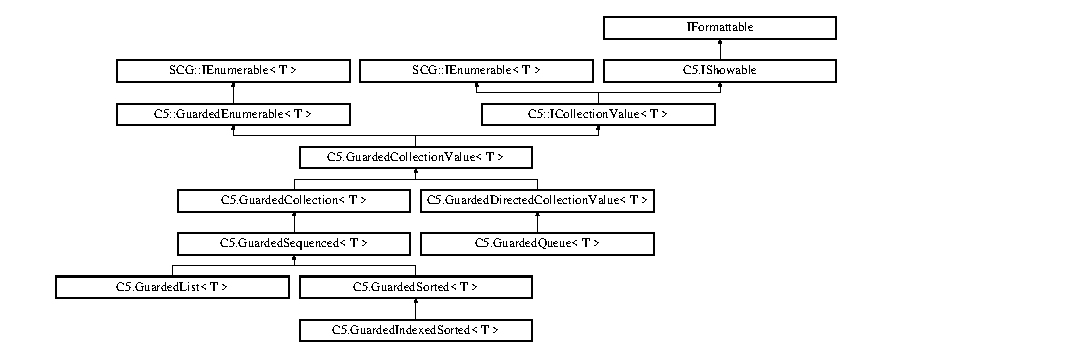
\includegraphics[height=4.357976cm]{class_c5_1_1_guarded_collection_value}
\end{center}
\end{figure}
\subsection*{Public Member Functions}
\begin{DoxyCompactItemize}
\item 
\hyperlink{class_c5_1_1_guarded_collection_value_ae5023d32e21e4f2a340f6b3dc49ffc47}{Guarded\+Collection\+Value} (\hyperlink{interface_c5_1_1_i_collection_value}{I\+Collection\+Value}$<$ T $>$ collectionvalue)
\begin{DoxyCompactList}\small\item\em Wrap a \hyperlink{interface_c5_1_1_i_collection_value}{I\+Collection\+Value}$<$T$>$ in a read-\/only wrapper \end{DoxyCompactList}\item 
virtual void \hyperlink{class_c5_1_1_guarded_collection_value_ae8d04b8fd3c59fe20bdc4a99fb1134f2}{Copy\+To} (T\mbox{[}$\,$\mbox{]} a, int i)
\begin{DoxyCompactList}\small\item\em Copy the items of the wrapped collection to an array \end{DoxyCompactList}\item 
virtual T\mbox{[}$\,$\mbox{]} \hyperlink{class_c5_1_1_guarded_collection_value_ab492c6c9d057b13d2ccbb7ebc259a4f6}{To\+Array} ()
\begin{DoxyCompactList}\small\item\em Create an array from the items of the wrapped collection \end{DoxyCompactList}\item 
virtual void \hyperlink{class_c5_1_1_guarded_collection_value_a212d1ea950a6096f846987476c9e2aa6}{Apply} (Action$<$ T $>$ a)
\begin{DoxyCompactList}\small\item\em Apply a delegate to all items of the wrapped enumerable. \end{DoxyCompactList}\item 
virtual bool \hyperlink{class_c5_1_1_guarded_collection_value_a0c3c6dfb00cd3206e56939a8a49ff622}{Exists} (Func$<$ T, bool $>$ filter)
\begin{DoxyCompactList}\small\item\em Check if there exists an item that satisfies a specific predicate in the wrapped enumerable. \end{DoxyCompactList}\item 
virtual bool \hyperlink{class_c5_1_1_guarded_collection_value_a7bccfb81326892afd0ae30ac5e55cdaa}{Find} (Func$<$ T, bool $>$ filter, out T item)
\item 
virtual bool \hyperlink{class_c5_1_1_guarded_collection_value_a0fda465306c55a4dde41b5eecdb1180a}{All} (Func$<$ T, bool $>$ filter)
\begin{DoxyCompactList}\small\item\em Check if all items in the wrapped enumerable satisfies a specific predicate. \end{DoxyCompactList}\item 
virtual S\+C\+G.\+I\+Enumerable$<$ T $>$ \hyperlink{class_c5_1_1_guarded_collection_value_a69ab914af51ee2fefc9a0e874e544b3f}{Filter} (Func$<$ T, bool $>$ filter)
\begin{DoxyCompactList}\small\item\em Create an enumerable, enumerating the items of this collection that satisfies a certain condition. \end{DoxyCompactList}\item 
virtual T \hyperlink{class_c5_1_1_guarded_collection_value_ac1c427d873e650f819d6c662515dadd1}{Choose} ()
\begin{DoxyCompactList}\small\item\em Choose some item of this collection. \end{DoxyCompactList}\item 
bool \hyperlink{class_c5_1_1_guarded_collection_value_afa61d34466d122adfde482979c147e9c}{Show} (System.\+Text.\+String\+Builder stringbuilder, ref int rest, I\+Format\+Provider format\+Provider)
\item 
string \hyperlink{class_c5_1_1_guarded_collection_value_aa77b66d63ed61af80e8bffbfb86a6929}{To\+String} (string format, I\+Format\+Provider format\+Provider)
\end{DoxyCompactItemize}
\subsection*{Properties}
\begin{DoxyCompactItemize}
\item 
virtual \hyperlink{namespace_c5_a9143bfd561fffa025d21561674758008}{Event\+Type\+Enum} \hyperlink{class_c5_1_1_guarded_collection_value_ae25ccc848da34d751250986e82f56faa}{Listenable\+Events}\hspace{0.3cm}{\ttfamily  \mbox{[}get\mbox{]}}
\begin{DoxyCompactList}\small\item\em The Listenable\+Events value of the wrapped collection \end{DoxyCompactList}\item 
virtual \hyperlink{namespace_c5_a9143bfd561fffa025d21561674758008}{Event\+Type\+Enum} \hyperlink{class_c5_1_1_guarded_collection_value_af2f6e3f9dac82651c997ea9b94fffe46}{Active\+Events}\hspace{0.3cm}{\ttfamily  \mbox{[}get\mbox{]}}
\begin{DoxyCompactList}\small\item\em The Active\+Events value of the wrapped collection \end{DoxyCompactList}\item 
Collection\+Changed\+Handler$<$ T $>$ \hyperlink{class_c5_1_1_guarded_collection_value_a38a7720b5a831f9db428150c9a919705}{Collection\+Changed}
\begin{DoxyCompactList}\small\item\em The change event. Will be raised for every change operation on the collection. \end{DoxyCompactList}\item 
Collection\+Cleared\+Handler$<$ T $>$ \hyperlink{class_c5_1_1_guarded_collection_value_a380426d2c8a2a3b02ec8f9ef7deafdc3}{Collection\+Cleared}
\begin{DoxyCompactList}\small\item\em The change event. Will be raised for every change operation on the collection. \end{DoxyCompactList}\item 
Items\+Added\+Handler$<$ T $>$ \hyperlink{class_c5_1_1_guarded_collection_value_aeb91b9e7ca3dfac470295adc96ab1dab}{Items\+Added}
\begin{DoxyCompactList}\small\item\em The item added event. Will be raised for every individual addition to the collection. \end{DoxyCompactList}\item 
Item\+Inserted\+Handler$<$ T $>$ \hyperlink{class_c5_1_1_guarded_collection_value_a3f96014a551bc419ff392b0603c5ea9b}{Item\+Inserted}
\begin{DoxyCompactList}\small\item\em The item added event. Will be raised for every individual addition to the collection. \end{DoxyCompactList}\item 
Items\+Removed\+Handler$<$ T $>$ \hyperlink{class_c5_1_1_guarded_collection_value_a85c761ac148d451a9bfc35647c4828fe}{Items\+Removed}
\begin{DoxyCompactList}\small\item\em The item removed event. Will be raised for every individual removal from the collection. \end{DoxyCompactList}\item 
Item\+Removed\+At\+Handler$<$ T $>$ \hyperlink{class_c5_1_1_guarded_collection_value_ae775067415ed075eab5ff22ed0cde2a4}{Item\+Removed\+At}
\begin{DoxyCompactList}\small\item\em The item removed event. Will be raised for every individual removal from the collection. \end{DoxyCompactList}\item 
virtual bool \hyperlink{class_c5_1_1_guarded_collection_value_aa567bdb55eab9d39405e1c09091afdbd}{Is\+Empty}\hspace{0.3cm}{\ttfamily  \mbox{[}get\mbox{]}}
\begin{DoxyCompactList}\small\item\em Get the size of the wrapped collection \end{DoxyCompactList}\item 
virtual int \hyperlink{class_c5_1_1_guarded_collection_value_a88d2c0a3a91c948b46417c1e60b45d44}{Count}\hspace{0.3cm}{\ttfamily  \mbox{[}get\mbox{]}}
\begin{DoxyCompactList}\small\item\em Get the size of the wrapped collection \end{DoxyCompactList}\item 
virtual \hyperlink{namespace_c5_a615ba88dcdaa8d5a3c5f833a73d7fad6}{Speed} \hyperlink{class_c5_1_1_guarded_collection_value_a1faa5213b85114c0611a39744edf8887}{Count\+Speed}\hspace{0.3cm}{\ttfamily  \mbox{[}get\mbox{]}}
\begin{DoxyCompactList}\small\item\em The value is symbolic indicating the type of asymptotic complexity in terms of the size of this collection (worst-\/case or amortized as relevant). \end{DoxyCompactList}\end{DoxyCompactItemize}
\subsection*{Additional Inherited Members}


\subsection{Detailed Description}
A read-\/only wrapper for an \hyperlink{interface_c5_1_1_i_collection_value}{I\+Collection\+Value}$<$T$>$ 

{\itshape This is mainly interesting as a base of other guard classes} 

\subsection{Constructor \& Destructor Documentation}
\hypertarget{class_c5_1_1_guarded_collection_value_ae5023d32e21e4f2a340f6b3dc49ffc47}{}\index{C5\+::\+Guarded\+Collection\+Value@{C5\+::\+Guarded\+Collection\+Value}!Guarded\+Collection\+Value@{Guarded\+Collection\+Value}}
\index{Guarded\+Collection\+Value@{Guarded\+Collection\+Value}!C5\+::\+Guarded\+Collection\+Value@{C5\+::\+Guarded\+Collection\+Value}}
\subsubsection[{Guarded\+Collection\+Value(\+I\+Collection\+Value$<$ T $>$ collectionvalue)}]{\setlength{\rightskip}{0pt plus 5cm}{\bf C5.\+Guarded\+Collection\+Value}$<$ T $>$.{\bf Guarded\+Collection\+Value} (
\begin{DoxyParamCaption}
\item[{{\bf I\+Collection\+Value}$<$ T $>$}]{collectionvalue}
\end{DoxyParamCaption}
)}\label{class_c5_1_1_guarded_collection_value_ae5023d32e21e4f2a340f6b3dc49ffc47}


Wrap a \hyperlink{interface_c5_1_1_i_collection_value}{I\+Collection\+Value}$<$T$>$ in a read-\/only wrapper 


\begin{DoxyParams}{Parameters}
{\em collectionvalue} & the collection to wrap\\
\hline
\end{DoxyParams}


\subsection{Member Function Documentation}
\hypertarget{class_c5_1_1_guarded_collection_value_a0fda465306c55a4dde41b5eecdb1180a}{}\index{C5\+::\+Guarded\+Collection\+Value@{C5\+::\+Guarded\+Collection\+Value}!All@{All}}
\index{All@{All}!C5\+::\+Guarded\+Collection\+Value@{C5\+::\+Guarded\+Collection\+Value}}
\subsubsection[{All(\+Func$<$ T, bool $>$ filter)}]{\setlength{\rightskip}{0pt plus 5cm}virtual bool {\bf C5.\+Guarded\+Collection\+Value}$<$ T $>$.All (
\begin{DoxyParamCaption}
\item[{Func$<$ T, bool $>$}]{filter}
\end{DoxyParamCaption}
)\hspace{0.3cm}{\ttfamily [virtual]}}\label{class_c5_1_1_guarded_collection_value_a0fda465306c55a4dde41b5eecdb1180a}


Check if all items in the wrapped enumerable satisfies a specific predicate. 


\begin{DoxyParams}{Parameters}
{\em filter} & A filter delegate (T\+:\+C5.\+Filter`1) defining the predicate\\
\hline
\end{DoxyParams}
\begin{DoxyReturn}{Returns}
True if all items satisfies the predicate
\end{DoxyReturn}


Implements \hyperlink{interface_c5_1_1_i_collection_value_a099c3a257e5c0b7212e34e52a4a4bda2}{C5.\+I\+Collection\+Value$<$ T $>$}.

\hypertarget{class_c5_1_1_guarded_collection_value_a212d1ea950a6096f846987476c9e2aa6}{}\index{C5\+::\+Guarded\+Collection\+Value@{C5\+::\+Guarded\+Collection\+Value}!Apply@{Apply}}
\index{Apply@{Apply}!C5\+::\+Guarded\+Collection\+Value@{C5\+::\+Guarded\+Collection\+Value}}
\subsubsection[{Apply(\+Action$<$ T $>$ a)}]{\setlength{\rightskip}{0pt plus 5cm}virtual void {\bf C5.\+Guarded\+Collection\+Value}$<$ T $>$.Apply (
\begin{DoxyParamCaption}
\item[{Action$<$ T $>$}]{a}
\end{DoxyParamCaption}
)\hspace{0.3cm}{\ttfamily [virtual]}}\label{class_c5_1_1_guarded_collection_value_a212d1ea950a6096f846987476c9e2aa6}


Apply a delegate to all items of the wrapped enumerable. 


\begin{DoxyParams}{Parameters}
{\em a} & The delegate to apply\\
\hline
\end{DoxyParams}


Implements \hyperlink{interface_c5_1_1_i_collection_value_aadcb9ce9d9362c0ade0c7d620e3cc182}{C5.\+I\+Collection\+Value$<$ T $>$}.

\hypertarget{class_c5_1_1_guarded_collection_value_ac1c427d873e650f819d6c662515dadd1}{}\index{C5\+::\+Guarded\+Collection\+Value@{C5\+::\+Guarded\+Collection\+Value}!Choose@{Choose}}
\index{Choose@{Choose}!C5\+::\+Guarded\+Collection\+Value@{C5\+::\+Guarded\+Collection\+Value}}
\subsubsection[{Choose()}]{\setlength{\rightskip}{0pt plus 5cm}virtual T {\bf C5.\+Guarded\+Collection\+Value}$<$ T $>$.Choose (
\begin{DoxyParamCaption}
{}
\end{DoxyParamCaption}
)\hspace{0.3cm}{\ttfamily [virtual]}}\label{class_c5_1_1_guarded_collection_value_ac1c427d873e650f819d6c662515dadd1}


Choose some item of this collection. 


\begin{DoxyExceptions}{Exceptions}
{\em \hyperlink{class_c5_1_1_no_such_item_exception}{No\+Such\+Item\+Exception}} & if collection is empty.\\
\hline
\end{DoxyExceptions}
\begin{DoxyReturn}{Returns}

\end{DoxyReturn}


Implements \hyperlink{interface_c5_1_1_i_collection_value_af72d52ddd8ea4130d508e1cf020cf7eb}{C5.\+I\+Collection\+Value$<$ T $>$}.

\hypertarget{class_c5_1_1_guarded_collection_value_ae8d04b8fd3c59fe20bdc4a99fb1134f2}{}\index{C5\+::\+Guarded\+Collection\+Value@{C5\+::\+Guarded\+Collection\+Value}!Copy\+To@{Copy\+To}}
\index{Copy\+To@{Copy\+To}!C5\+::\+Guarded\+Collection\+Value@{C5\+::\+Guarded\+Collection\+Value}}
\subsubsection[{Copy\+To(\+T[] a, int i)}]{\setlength{\rightskip}{0pt plus 5cm}virtual void {\bf C5.\+Guarded\+Collection\+Value}$<$ T $>$.Copy\+To (
\begin{DoxyParamCaption}
\item[{T\mbox{[}$\,$\mbox{]}}]{a, }
\item[{int}]{i}
\end{DoxyParamCaption}
)\hspace{0.3cm}{\ttfamily [virtual]}}\label{class_c5_1_1_guarded_collection_value_ae8d04b8fd3c59fe20bdc4a99fb1134f2}


Copy the items of the wrapped collection to an array 


\begin{DoxyParams}{Parameters}
{\em a} & The array\\
\hline
{\em i} & Starting offset\\
\hline
\end{DoxyParams}


Implements \hyperlink{interface_c5_1_1_i_collection_value_aced299d8dce69c33ff75b598e39581d1}{C5.\+I\+Collection\+Value$<$ T $>$}.

\hypertarget{class_c5_1_1_guarded_collection_value_a0c3c6dfb00cd3206e56939a8a49ff622}{}\index{C5\+::\+Guarded\+Collection\+Value@{C5\+::\+Guarded\+Collection\+Value}!Exists@{Exists}}
\index{Exists@{Exists}!C5\+::\+Guarded\+Collection\+Value@{C5\+::\+Guarded\+Collection\+Value}}
\subsubsection[{Exists(\+Func$<$ T, bool $>$ filter)}]{\setlength{\rightskip}{0pt plus 5cm}virtual bool {\bf C5.\+Guarded\+Collection\+Value}$<$ T $>$.Exists (
\begin{DoxyParamCaption}
\item[{Func$<$ T, bool $>$}]{filter}
\end{DoxyParamCaption}
)\hspace{0.3cm}{\ttfamily [virtual]}}\label{class_c5_1_1_guarded_collection_value_a0c3c6dfb00cd3206e56939a8a49ff622}


Check if there exists an item that satisfies a specific predicate in the wrapped enumerable. 


\begin{DoxyParams}{Parameters}
{\em filter} & A filter delegate (T\+:\+C5.\+Filter`1) defining the predicate\\
\hline
\end{DoxyParams}
\begin{DoxyReturn}{Returns}
True is such an item exists
\end{DoxyReturn}


Implements \hyperlink{interface_c5_1_1_i_collection_value_a3c20f35782dbd046f9aba5ec13dad789}{C5.\+I\+Collection\+Value$<$ T $>$}.

\hypertarget{class_c5_1_1_guarded_collection_value_a69ab914af51ee2fefc9a0e874e544b3f}{}\index{C5\+::\+Guarded\+Collection\+Value@{C5\+::\+Guarded\+Collection\+Value}!Filter@{Filter}}
\index{Filter@{Filter}!C5\+::\+Guarded\+Collection\+Value@{C5\+::\+Guarded\+Collection\+Value}}
\subsubsection[{Filter(\+Func$<$ T, bool $>$ filter)}]{\setlength{\rightskip}{0pt plus 5cm}virtual S\+C\+G.\+I\+Enumerable$<$T$>$ {\bf C5.\+Guarded\+Collection\+Value}$<$ T $>$.Filter (
\begin{DoxyParamCaption}
\item[{Func$<$ T, bool $>$}]{filter}
\end{DoxyParamCaption}
)\hspace{0.3cm}{\ttfamily [virtual]}}\label{class_c5_1_1_guarded_collection_value_a69ab914af51ee2fefc9a0e874e544b3f}


Create an enumerable, enumerating the items of this collection that satisfies a certain condition. 


\begin{DoxyParams}{Parameters}
{\em filter} & The T-\/$>$bool filter delegate defining the condition\\
\hline
\end{DoxyParams}
\begin{DoxyReturn}{Returns}
The filtered enumerable
\end{DoxyReturn}


Implements \hyperlink{interface_c5_1_1_i_collection_value_a485e8b464ed5dfb5f2ff5dc10a8a62d6}{C5.\+I\+Collection\+Value$<$ T $>$}.

\hypertarget{class_c5_1_1_guarded_collection_value_a7bccfb81326892afd0ae30ac5e55cdaa}{}\index{C5\+::\+Guarded\+Collection\+Value@{C5\+::\+Guarded\+Collection\+Value}!Find@{Find}}
\index{Find@{Find}!C5\+::\+Guarded\+Collection\+Value@{C5\+::\+Guarded\+Collection\+Value}}
\subsubsection[{Find(\+Func$<$ T, bool $>$ filter, out T item)}]{\setlength{\rightskip}{0pt plus 5cm}virtual bool {\bf C5.\+Guarded\+Collection\+Value}$<$ T $>$.Find (
\begin{DoxyParamCaption}
\item[{Func$<$ T, bool $>$}]{filter, }
\item[{out T}]{item}
\end{DoxyParamCaption}
)\hspace{0.3cm}{\ttfamily [virtual]}}\label{class_c5_1_1_guarded_collection_value_a7bccfb81326892afd0ae30ac5e55cdaa}





\begin{DoxyParams}{Parameters}
{\em filter} & \\
\hline
{\em item} & \\
\hline
\end{DoxyParams}
\begin{DoxyReturn}{Returns}

\end{DoxyReturn}


Implements \hyperlink{interface_c5_1_1_i_collection_value_a3e175f833398fa6a6cde45e4948bc152}{C5.\+I\+Collection\+Value$<$ T $>$}.

\hypertarget{class_c5_1_1_guarded_collection_value_afa61d34466d122adfde482979c147e9c}{}\index{C5\+::\+Guarded\+Collection\+Value@{C5\+::\+Guarded\+Collection\+Value}!Show@{Show}}
\index{Show@{Show}!C5\+::\+Guarded\+Collection\+Value@{C5\+::\+Guarded\+Collection\+Value}}
\subsubsection[{Show(\+System.\+Text.\+String\+Builder stringbuilder, ref int rest, I\+Format\+Provider format\+Provider)}]{\setlength{\rightskip}{0pt plus 5cm}bool {\bf C5.\+Guarded\+Collection\+Value}$<$ T $>$.Show (
\begin{DoxyParamCaption}
\item[{System.\+Text.\+String\+Builder}]{stringbuilder, }
\item[{ref int}]{rest, }
\item[{I\+Format\+Provider}]{format\+Provider}
\end{DoxyParamCaption}
)}\label{class_c5_1_1_guarded_collection_value_afa61d34466d122adfde482979c147e9c}





\begin{DoxyParams}{Parameters}
{\em stringbuilder} & \\
\hline
{\em format\+Provider} & \\
\hline
{\em rest} & \\
\hline
\end{DoxyParams}
\begin{DoxyReturn}{Returns}

\end{DoxyReturn}
\hypertarget{class_c5_1_1_guarded_collection_value_ab492c6c9d057b13d2ccbb7ebc259a4f6}{}\index{C5\+::\+Guarded\+Collection\+Value@{C5\+::\+Guarded\+Collection\+Value}!To\+Array@{To\+Array}}
\index{To\+Array@{To\+Array}!C5\+::\+Guarded\+Collection\+Value@{C5\+::\+Guarded\+Collection\+Value}}
\subsubsection[{To\+Array()}]{\setlength{\rightskip}{0pt plus 5cm}virtual T \mbox{[}$\,$\mbox{]} {\bf C5.\+Guarded\+Collection\+Value}$<$ T $>$.To\+Array (
\begin{DoxyParamCaption}
{}
\end{DoxyParamCaption}
)\hspace{0.3cm}{\ttfamily [virtual]}}\label{class_c5_1_1_guarded_collection_value_ab492c6c9d057b13d2ccbb7ebc259a4f6}


Create an array from the items of the wrapped collection 

\begin{DoxyReturn}{Returns}
The array
\end{DoxyReturn}


Implements \hyperlink{interface_c5_1_1_i_collection_value_ad76547324e71a04e92076b2e55239bbb}{C5.\+I\+Collection\+Value$<$ T $>$}.

\hypertarget{class_c5_1_1_guarded_collection_value_aa77b66d63ed61af80e8bffbfb86a6929}{}\index{C5\+::\+Guarded\+Collection\+Value@{C5\+::\+Guarded\+Collection\+Value}!To\+String@{To\+String}}
\index{To\+String@{To\+String}!C5\+::\+Guarded\+Collection\+Value@{C5\+::\+Guarded\+Collection\+Value}}
\subsubsection[{To\+String(string format, I\+Format\+Provider format\+Provider)}]{\setlength{\rightskip}{0pt plus 5cm}string {\bf C5.\+Guarded\+Collection\+Value}$<$ T $>$.To\+String (
\begin{DoxyParamCaption}
\item[{string}]{format, }
\item[{I\+Format\+Provider}]{format\+Provider}
\end{DoxyParamCaption}
)}\label{class_c5_1_1_guarded_collection_value_aa77b66d63ed61af80e8bffbfb86a6929}





\begin{DoxyParams}{Parameters}
{\em format} & \\
\hline
{\em format\+Provider} & \\
\hline
\end{DoxyParams}
\begin{DoxyReturn}{Returns}

\end{DoxyReturn}


\subsection{Property Documentation}
\hypertarget{class_c5_1_1_guarded_collection_value_af2f6e3f9dac82651c997ea9b94fffe46}{}\index{C5\+::\+Guarded\+Collection\+Value@{C5\+::\+Guarded\+Collection\+Value}!Active\+Events@{Active\+Events}}
\index{Active\+Events@{Active\+Events}!C5\+::\+Guarded\+Collection\+Value@{C5\+::\+Guarded\+Collection\+Value}}
\subsubsection[{Active\+Events}]{\setlength{\rightskip}{0pt plus 5cm}virtual {\bf Event\+Type\+Enum} {\bf C5.\+Guarded\+Collection\+Value}$<$ T $>$.Active\+Events\hspace{0.3cm}{\ttfamily [get]}}\label{class_c5_1_1_guarded_collection_value_af2f6e3f9dac82651c997ea9b94fffe46}


The Active\+Events value of the wrapped collection 

\hypertarget{class_c5_1_1_guarded_collection_value_a38a7720b5a831f9db428150c9a919705}{}\index{C5\+::\+Guarded\+Collection\+Value@{C5\+::\+Guarded\+Collection\+Value}!Collection\+Changed@{Collection\+Changed}}
\index{Collection\+Changed@{Collection\+Changed}!C5\+::\+Guarded\+Collection\+Value@{C5\+::\+Guarded\+Collection\+Value}}
\subsubsection[{Collection\+Changed}]{\setlength{\rightskip}{0pt plus 5cm}Collection\+Changed\+Handler$<$T$>$ {\bf C5.\+Guarded\+Collection\+Value}$<$ T $>$.Collection\+Changed\hspace{0.3cm}{\ttfamily [add]}, {\ttfamily [remove]}}\label{class_c5_1_1_guarded_collection_value_a38a7720b5a831f9db428150c9a919705}


The change event. Will be raised for every change operation on the collection. 

\hypertarget{class_c5_1_1_guarded_collection_value_a380426d2c8a2a3b02ec8f9ef7deafdc3}{}\index{C5\+::\+Guarded\+Collection\+Value@{C5\+::\+Guarded\+Collection\+Value}!Collection\+Cleared@{Collection\+Cleared}}
\index{Collection\+Cleared@{Collection\+Cleared}!C5\+::\+Guarded\+Collection\+Value@{C5\+::\+Guarded\+Collection\+Value}}
\subsubsection[{Collection\+Cleared}]{\setlength{\rightskip}{0pt plus 5cm}Collection\+Cleared\+Handler$<$T$>$ {\bf C5.\+Guarded\+Collection\+Value}$<$ T $>$.Collection\+Cleared\hspace{0.3cm}{\ttfamily [add]}, {\ttfamily [remove]}}\label{class_c5_1_1_guarded_collection_value_a380426d2c8a2a3b02ec8f9ef7deafdc3}


The change event. Will be raised for every change operation on the collection. 

\hypertarget{class_c5_1_1_guarded_collection_value_a88d2c0a3a91c948b46417c1e60b45d44}{}\index{C5\+::\+Guarded\+Collection\+Value@{C5\+::\+Guarded\+Collection\+Value}!Count@{Count}}
\index{Count@{Count}!C5\+::\+Guarded\+Collection\+Value@{C5\+::\+Guarded\+Collection\+Value}}
\subsubsection[{Count}]{\setlength{\rightskip}{0pt plus 5cm}virtual int {\bf C5.\+Guarded\+Collection\+Value}$<$ T $>$.Count\hspace{0.3cm}{\ttfamily [get]}}\label{class_c5_1_1_guarded_collection_value_a88d2c0a3a91c948b46417c1e60b45d44}


Get the size of the wrapped collection 

The size\hypertarget{class_c5_1_1_guarded_collection_value_a1faa5213b85114c0611a39744edf8887}{}\index{C5\+::\+Guarded\+Collection\+Value@{C5\+::\+Guarded\+Collection\+Value}!Count\+Speed@{Count\+Speed}}
\index{Count\+Speed@{Count\+Speed}!C5\+::\+Guarded\+Collection\+Value@{C5\+::\+Guarded\+Collection\+Value}}
\subsubsection[{Count\+Speed}]{\setlength{\rightskip}{0pt plus 5cm}virtual {\bf Speed} {\bf C5.\+Guarded\+Collection\+Value}$<$ T $>$.Count\+Speed\hspace{0.3cm}{\ttfamily [get]}}\label{class_c5_1_1_guarded_collection_value_a1faa5213b85114c0611a39744edf8887}


The value is symbolic indicating the type of asymptotic complexity in terms of the size of this collection (worst-\/case or amortized as relevant). 

A characterization of the speed of the {\ttfamily Count} property in this collection.\hypertarget{class_c5_1_1_guarded_collection_value_aa567bdb55eab9d39405e1c09091afdbd}{}\index{C5\+::\+Guarded\+Collection\+Value@{C5\+::\+Guarded\+Collection\+Value}!Is\+Empty@{Is\+Empty}}
\index{Is\+Empty@{Is\+Empty}!C5\+::\+Guarded\+Collection\+Value@{C5\+::\+Guarded\+Collection\+Value}}
\subsubsection[{Is\+Empty}]{\setlength{\rightskip}{0pt plus 5cm}virtual bool {\bf C5.\+Guarded\+Collection\+Value}$<$ T $>$.Is\+Empty\hspace{0.3cm}{\ttfamily [get]}}\label{class_c5_1_1_guarded_collection_value_aa567bdb55eab9d39405e1c09091afdbd}


Get the size of the wrapped collection 

The size\hypertarget{class_c5_1_1_guarded_collection_value_a3f96014a551bc419ff392b0603c5ea9b}{}\index{C5\+::\+Guarded\+Collection\+Value@{C5\+::\+Guarded\+Collection\+Value}!Item\+Inserted@{Item\+Inserted}}
\index{Item\+Inserted@{Item\+Inserted}!C5\+::\+Guarded\+Collection\+Value@{C5\+::\+Guarded\+Collection\+Value}}
\subsubsection[{Item\+Inserted}]{\setlength{\rightskip}{0pt plus 5cm}Item\+Inserted\+Handler$<$T$>$ {\bf C5.\+Guarded\+Collection\+Value}$<$ T $>$.Item\+Inserted\hspace{0.3cm}{\ttfamily [add]}, {\ttfamily [remove]}}\label{class_c5_1_1_guarded_collection_value_a3f96014a551bc419ff392b0603c5ea9b}


The item added event. Will be raised for every individual addition to the collection. 

\hypertarget{class_c5_1_1_guarded_collection_value_ae775067415ed075eab5ff22ed0cde2a4}{}\index{C5\+::\+Guarded\+Collection\+Value@{C5\+::\+Guarded\+Collection\+Value}!Item\+Removed\+At@{Item\+Removed\+At}}
\index{Item\+Removed\+At@{Item\+Removed\+At}!C5\+::\+Guarded\+Collection\+Value@{C5\+::\+Guarded\+Collection\+Value}}
\subsubsection[{Item\+Removed\+At}]{\setlength{\rightskip}{0pt plus 5cm}Item\+Removed\+At\+Handler$<$T$>$ {\bf C5.\+Guarded\+Collection\+Value}$<$ T $>$.Item\+Removed\+At\hspace{0.3cm}{\ttfamily [add]}, {\ttfamily [remove]}}\label{class_c5_1_1_guarded_collection_value_ae775067415ed075eab5ff22ed0cde2a4}


The item removed event. Will be raised for every individual removal from the collection. 

\hypertarget{class_c5_1_1_guarded_collection_value_aeb91b9e7ca3dfac470295adc96ab1dab}{}\index{C5\+::\+Guarded\+Collection\+Value@{C5\+::\+Guarded\+Collection\+Value}!Items\+Added@{Items\+Added}}
\index{Items\+Added@{Items\+Added}!C5\+::\+Guarded\+Collection\+Value@{C5\+::\+Guarded\+Collection\+Value}}
\subsubsection[{Items\+Added}]{\setlength{\rightskip}{0pt plus 5cm}Items\+Added\+Handler$<$T$>$ {\bf C5.\+Guarded\+Collection\+Value}$<$ T $>$.Items\+Added\hspace{0.3cm}{\ttfamily [add]}, {\ttfamily [remove]}}\label{class_c5_1_1_guarded_collection_value_aeb91b9e7ca3dfac470295adc96ab1dab}


The item added event. Will be raised for every individual addition to the collection. 

\hypertarget{class_c5_1_1_guarded_collection_value_a85c761ac148d451a9bfc35647c4828fe}{}\index{C5\+::\+Guarded\+Collection\+Value@{C5\+::\+Guarded\+Collection\+Value}!Items\+Removed@{Items\+Removed}}
\index{Items\+Removed@{Items\+Removed}!C5\+::\+Guarded\+Collection\+Value@{C5\+::\+Guarded\+Collection\+Value}}
\subsubsection[{Items\+Removed}]{\setlength{\rightskip}{0pt plus 5cm}Items\+Removed\+Handler$<$T$>$ {\bf C5.\+Guarded\+Collection\+Value}$<$ T $>$.Items\+Removed\hspace{0.3cm}{\ttfamily [add]}, {\ttfamily [remove]}}\label{class_c5_1_1_guarded_collection_value_a85c761ac148d451a9bfc35647c4828fe}


The item removed event. Will be raised for every individual removal from the collection. 

\hypertarget{class_c5_1_1_guarded_collection_value_ae25ccc848da34d751250986e82f56faa}{}\index{C5\+::\+Guarded\+Collection\+Value@{C5\+::\+Guarded\+Collection\+Value}!Listenable\+Events@{Listenable\+Events}}
\index{Listenable\+Events@{Listenable\+Events}!C5\+::\+Guarded\+Collection\+Value@{C5\+::\+Guarded\+Collection\+Value}}
\subsubsection[{Listenable\+Events}]{\setlength{\rightskip}{0pt plus 5cm}virtual {\bf Event\+Type\+Enum} {\bf C5.\+Guarded\+Collection\+Value}$<$ T $>$.Listenable\+Events\hspace{0.3cm}{\ttfamily [get]}}\label{class_c5_1_1_guarded_collection_value_ae25ccc848da34d751250986e82f56faa}


The Listenable\+Events value of the wrapped collection 



The documentation for this class was generated from the following file\+:\begin{DoxyCompactItemize}
\item 
C\+:/\+Users/rasmusl/\+Source/\+Repos/\+C5/\+C5/\hyperlink{_wrappers_8cs}{Wrappers.\+cs}\end{DoxyCompactItemize}

\hypertarget{class_c5_1_1_guarded_dictionary}{}\section{C5.\+Guarded\+Dictionary$<$ K, V $>$ Class Template Reference}
\label{class_c5_1_1_guarded_dictionary}\index{C5.\+Guarded\+Dictionary$<$ K, V $>$@{C5.\+Guarded\+Dictionary$<$ K, V $>$}}


A read-\/only wrapper for a dictionary.  


Inheritance diagram for C5.\+Guarded\+Dictionary$<$ K, V $>$\+:\begin{figure}[H]
\begin{center}
\leavevmode
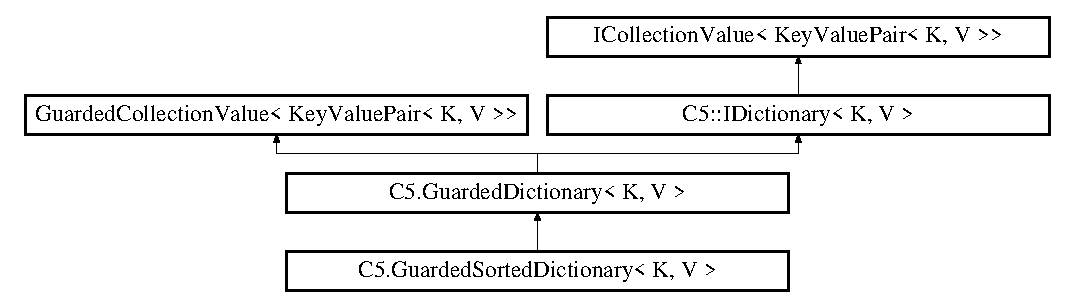
\includegraphics[height=3.672131cm]{class_c5_1_1_guarded_dictionary}
\end{center}
\end{figure}
\subsection*{Public Member Functions}
\begin{DoxyCompactItemize}
\item 
\hyperlink{class_c5_1_1_guarded_dictionary_aede5f0b863aa1b9e73aaefc75b07406b}{Guarded\+Dictionary} (\hyperlink{interface_c5_1_1_i_dictionary}{I\+Dictionary}$<$ K, V $>$ dict)
\begin{DoxyCompactList}\small\item\em Wrap a dictionary in a read-\/only wrapper \end{DoxyCompactList}\item 
void \hyperlink{class_c5_1_1_guarded_dictionary_a353f8b07283f31fb34456317bdb9cf43}{Add} (K key, V val)
\item 
void \hyperlink{class_c5_1_1_guarded_dictionary_a992dd8a21a6a6146fc937d0975ee1c8a}{Add\+All$<$ L, W $>$} (S\+C\+G.\+I\+Enumerable$<$ \hyperlink{struct_c5_1_1_key_value_pair}{Key\+Value\+Pair}$<$ L, W $>$$>$ items)
\item 
bool \hyperlink{class_c5_1_1_guarded_dictionary_a80c9ecc7aa9664fbcd7e292bda4342bc}{Remove} (K key)
\item 
bool \hyperlink{class_c5_1_1_guarded_dictionary_a854f4f5d586a5712b4b96268ac63950b}{Remove} (K key, out V val)
\item 
void \hyperlink{class_c5_1_1_guarded_dictionary_ac5f23f523e9eae132f4e465eb004be0a}{Clear} ()
\item 
bool \hyperlink{class_c5_1_1_guarded_dictionary_a16126875960f6459a2d697131755128c}{Contains} (K key)
\begin{DoxyCompactList}\small\item\em Check if the wrapped dictionary contains a specific key \end{DoxyCompactList}\item 
bool \hyperlink{class_c5_1_1_guarded_dictionary_aba0b4712e17daaba4b81245cc6958862}{Contains\+All$<$ H $>$} (S\+C\+G.\+I\+Enumerable$<$ H $>$ keys)
\item 
bool \hyperlink{class_c5_1_1_guarded_dictionary_af7eef747a8e733e4167c1a9ea4954274}{Find} (ref K key, out V val)
\begin{DoxyCompactList}\small\item\em Search for a key in the wrapped dictionary, reporting the value if found \end{DoxyCompactList}\item 
bool \hyperlink{class_c5_1_1_guarded_dictionary_a128b6b9f09658c7cd687248592197669}{Update} (K key, V val)
\item 
bool \hyperlink{class_c5_1_1_guarded_dictionary_a74de4c990cdc8e7b5245d2931c71274e}{Update} (K key, V val, out V oldval)
\item 
bool \hyperlink{class_c5_1_1_guarded_dictionary_ab276e6b0828e40022f2b3ef39e22305c}{Find\+Or\+Add} (K key, ref V val)
\item 
bool \hyperlink{class_c5_1_1_guarded_dictionary_a4d75103d8bfec4c044a22ed8ec7fdf46}{Update\+Or\+Add} (K key, V val)
\item 
bool \hyperlink{class_c5_1_1_guarded_dictionary_a8b6c55913a3f297ea9579800a9be6580}{Update\+Or\+Add} (K key, V val, out V oldval)
\item 
bool \hyperlink{class_c5_1_1_guarded_dictionary_a366d84d2fd3b966b091e030cd8ff131b}{Check} ()
\begin{DoxyCompactList}\small\item\em Check the internal consistency of the wrapped dictionary \end{DoxyCompactList}\end{DoxyCompactItemize}
\subsection*{Properties}
\begin{DoxyCompactItemize}
\item 
S\+C\+G.\+I\+Equality\+Comparer$<$ K $>$ \hyperlink{class_c5_1_1_guarded_dictionary_aa92bdc349fb14d43d5ead652ec07e3fa}{Equality\+Comparer}\hspace{0.3cm}{\ttfamily  \mbox{[}get\mbox{]}}
\item 
V \hyperlink{class_c5_1_1_guarded_dictionary_a721d36a134e3aa6ff2c92cf6bffb9fb3}{this\mbox{[}\+K key\mbox{]}}\hspace{0.3cm}{\ttfamily  \mbox{[}get, set\mbox{]}}
\item 
bool \hyperlink{class_c5_1_1_guarded_dictionary_a18ce63220c7b6b3e6a569cd321c4da16}{Is\+Read\+Only}\hspace{0.3cm}{\ttfamily  \mbox{[}get\mbox{]}}
\begin{DoxyCompactList}\small\item\em (This is a read-\/only wrapper) \end{DoxyCompactList}\item 
\hyperlink{interface_c5_1_1_i_collection_value}{I\+Collection\+Value}$<$ K $>$ \hyperlink{class_c5_1_1_guarded_dictionary_a9ebe83dbe1e0e8c93c7d268c3643fba4}{Keys}\hspace{0.3cm}{\ttfamily  \mbox{[}get\mbox{]}}
\item 
\hyperlink{interface_c5_1_1_i_collection_value}{I\+Collection\+Value}$<$ V $>$ \hyperlink{class_c5_1_1_guarded_dictionary_ab5aef218f548d9a8abb97ff033be4173}{Values}\hspace{0.3cm}{\ttfamily  \mbox{[}get\mbox{]}}
\item 
virtual Func$<$ K, V $>$ \hyperlink{class_c5_1_1_guarded_dictionary_a0dc7a885f47a6a2506e46fb813190231}{Func}\hspace{0.3cm}{\ttfamily  \mbox{[}get\mbox{]}}
\item 
\hyperlink{namespace_c5_a615ba88dcdaa8d5a3c5f833a73d7fad6}{Speed} \hyperlink{class_c5_1_1_guarded_dictionary_a4926964829c05063b557c42f6ed6f9e1}{Contains\+Speed}\hspace{0.3cm}{\ttfamily  \mbox{[}get\mbox{]}}
\end{DoxyCompactItemize}


\subsection{Detailed Description}
A read-\/only wrapper for a dictionary. 

{\itshape Suitable for wrapping a \hyperlink{class_c5_1_1_hash_dictionary}{Hash\+Dictionary}. T\+:\+C5.\+Hash\+Dictionary`2} 

\subsection{Constructor \& Destructor Documentation}
\hypertarget{class_c5_1_1_guarded_dictionary_aede5f0b863aa1b9e73aaefc75b07406b}{}\index{C5\+::\+Guarded\+Dictionary@{C5\+::\+Guarded\+Dictionary}!Guarded\+Dictionary@{Guarded\+Dictionary}}
\index{Guarded\+Dictionary@{Guarded\+Dictionary}!C5\+::\+Guarded\+Dictionary@{C5\+::\+Guarded\+Dictionary}}
\subsubsection[{Guarded\+Dictionary(\+I\+Dictionary$<$ K, V $>$ dict)}]{\setlength{\rightskip}{0pt plus 5cm}{\bf C5.\+Guarded\+Dictionary}$<$ K, V $>$.{\bf Guarded\+Dictionary} (
\begin{DoxyParamCaption}
\item[{{\bf I\+Dictionary}$<$ K, V $>$}]{dict}
\end{DoxyParamCaption}
)}\label{class_c5_1_1_guarded_dictionary_aede5f0b863aa1b9e73aaefc75b07406b}


Wrap a dictionary in a read-\/only wrapper 


\begin{DoxyParams}{Parameters}
{\em dict} & the dictionary\\
\hline
\end{DoxyParams}


\subsection{Member Function Documentation}
\hypertarget{class_c5_1_1_guarded_dictionary_a353f8b07283f31fb34456317bdb9cf43}{}\index{C5\+::\+Guarded\+Dictionary@{C5\+::\+Guarded\+Dictionary}!Add@{Add}}
\index{Add@{Add}!C5\+::\+Guarded\+Dictionary@{C5\+::\+Guarded\+Dictionary}}
\subsubsection[{Add(\+K key, V val)}]{\setlength{\rightskip}{0pt plus 5cm}void {\bf C5.\+Guarded\+Dictionary}$<$ K, V $>$.Add (
\begin{DoxyParamCaption}
\item[{K}]{key, }
\item[{V}]{val}
\end{DoxyParamCaption}
)}\label{class_c5_1_1_guarded_dictionary_a353f8b07283f31fb34456317bdb9cf43}





\begin{DoxyExceptions}{Exceptions}
{\em \hyperlink{class_c5_1_1_read_only_collection_exception}{Read\+Only\+Collection\+Exception}} & since this is a read-\/only wrappper\\
\hline
\end{DoxyExceptions}

\begin{DoxyParams}{Parameters}
{\em key} & \\
\hline
{\em val} & \\
\hline
\end{DoxyParams}


Implements \hyperlink{interface_c5_1_1_i_dictionary_a7e3eefcf603863fe54ce86080bbc07d7}{C5.\+I\+Dictionary$<$ K, V $>$}.

\hypertarget{class_c5_1_1_guarded_dictionary_a992dd8a21a6a6146fc937d0975ee1c8a}{}\index{C5\+::\+Guarded\+Dictionary@{C5\+::\+Guarded\+Dictionary}!Add\+All$<$ L, W $>$@{Add\+All$<$ L, W $>$}}
\index{Add\+All$<$ L, W $>$@{Add\+All$<$ L, W $>$}!C5\+::\+Guarded\+Dictionary@{C5\+::\+Guarded\+Dictionary}}
\subsubsection[{Add\+All$<$ L, W $>$(\+S\+C\+G.\+I\+Enumerable$<$ Key\+Value\+Pair$<$ L, W $>$$>$ items)}]{\setlength{\rightskip}{0pt plus 5cm}void {\bf C5.\+Guarded\+Dictionary}$<$ K, V $>$.Add\+All$<$ L, W $>$ (
\begin{DoxyParamCaption}
\item[{S\+C\+G.\+I\+Enumerable$<$ {\bf Key\+Value\+Pair}$<$ L, W $>$$>$}]{items}
\end{DoxyParamCaption}
)}\label{class_c5_1_1_guarded_dictionary_a992dd8a21a6a6146fc937d0975ee1c8a}





\begin{DoxyExceptions}{Exceptions}
{\em \hyperlink{class_c5_1_1_read_only_collection_exception}{Read\+Only\+Collection\+Exception}} & since this is a read-\/only wrappper\\
\hline
\end{DoxyExceptions}

\begin{DoxyParams}{Parameters}
{\em items} & \\
\hline
\end{DoxyParams}
\begin{Desc}
\item[Type Constraints]\begin{description}
\item[{\em L} : {\em K}]\item[{\em W} : {\em V}]\end{description}
\end{Desc}
\hypertarget{class_c5_1_1_guarded_dictionary_a366d84d2fd3b966b091e030cd8ff131b}{}\index{C5\+::\+Guarded\+Dictionary@{C5\+::\+Guarded\+Dictionary}!Check@{Check}}
\index{Check@{Check}!C5\+::\+Guarded\+Dictionary@{C5\+::\+Guarded\+Dictionary}}
\subsubsection[{Check()}]{\setlength{\rightskip}{0pt plus 5cm}bool {\bf C5.\+Guarded\+Dictionary}$<$ K, V $>$.Check (
\begin{DoxyParamCaption}
{}
\end{DoxyParamCaption}
)}\label{class_c5_1_1_guarded_dictionary_a366d84d2fd3b966b091e030cd8ff131b}


Check the internal consistency of the wrapped dictionary 

\begin{DoxyReturn}{Returns}
True if check passed
\end{DoxyReturn}


Implements \hyperlink{interface_c5_1_1_i_dictionary_a659969044740981cdcfe5ee86585104c}{C5.\+I\+Dictionary$<$ K, V $>$}.

\hypertarget{class_c5_1_1_guarded_dictionary_ac5f23f523e9eae132f4e465eb004be0a}{}\index{C5\+::\+Guarded\+Dictionary@{C5\+::\+Guarded\+Dictionary}!Clear@{Clear}}
\index{Clear@{Clear}!C5\+::\+Guarded\+Dictionary@{C5\+::\+Guarded\+Dictionary}}
\subsubsection[{Clear()}]{\setlength{\rightskip}{0pt plus 5cm}void {\bf C5.\+Guarded\+Dictionary}$<$ K, V $>$.Clear (
\begin{DoxyParamCaption}
{}
\end{DoxyParamCaption}
)}\label{class_c5_1_1_guarded_dictionary_ac5f23f523e9eae132f4e465eb004be0a}





\begin{DoxyExceptions}{Exceptions}
{\em \hyperlink{class_c5_1_1_read_only_collection_exception}{Read\+Only\+Collection\+Exception}} & since this is a read-\/only wrappper\\
\hline
\end{DoxyExceptions}


Implements \hyperlink{interface_c5_1_1_i_dictionary_a9eb0026921a6b39c781495efd65dc82b}{C5.\+I\+Dictionary$<$ K, V $>$}.

\hypertarget{class_c5_1_1_guarded_dictionary_a16126875960f6459a2d697131755128c}{}\index{C5\+::\+Guarded\+Dictionary@{C5\+::\+Guarded\+Dictionary}!Contains@{Contains}}
\index{Contains@{Contains}!C5\+::\+Guarded\+Dictionary@{C5\+::\+Guarded\+Dictionary}}
\subsubsection[{Contains(\+K key)}]{\setlength{\rightskip}{0pt plus 5cm}bool {\bf C5.\+Guarded\+Dictionary}$<$ K, V $>$.Contains (
\begin{DoxyParamCaption}
\item[{K}]{key}
\end{DoxyParamCaption}
)}\label{class_c5_1_1_guarded_dictionary_a16126875960f6459a2d697131755128c}


Check if the wrapped dictionary contains a specific key 


\begin{DoxyParams}{Parameters}
{\em key} & The key\\
\hline
\end{DoxyParams}
\begin{DoxyReturn}{Returns}
True if it does
\end{DoxyReturn}


Implements \hyperlink{interface_c5_1_1_i_dictionary_a08f4af4a7f427e8e9022a13f2e79c031}{C5.\+I\+Dictionary$<$ K, V $>$}.

\hypertarget{class_c5_1_1_guarded_dictionary_aba0b4712e17daaba4b81245cc6958862}{}\index{C5\+::\+Guarded\+Dictionary@{C5\+::\+Guarded\+Dictionary}!Contains\+All$<$ H $>$@{Contains\+All$<$ H $>$}}
\index{Contains\+All$<$ H $>$@{Contains\+All$<$ H $>$}!C5\+::\+Guarded\+Dictionary@{C5\+::\+Guarded\+Dictionary}}
\subsubsection[{Contains\+All$<$ H $>$(\+S\+C\+G.\+I\+Enumerable$<$ H $>$ keys)}]{\setlength{\rightskip}{0pt plus 5cm}bool {\bf C5.\+Guarded\+Dictionary}$<$ K, V $>$.Contains\+All$<$ H $>$ (
\begin{DoxyParamCaption}
\item[{S\+C\+G.\+I\+Enumerable$<$ H $>$}]{keys}
\end{DoxyParamCaption}
)}\label{class_c5_1_1_guarded_dictionary_aba0b4712e17daaba4b81245cc6958862}





\begin{DoxyParams}{Parameters}
{\em keys} & \\
\hline
\end{DoxyParams}
\begin{DoxyReturn}{Returns}

\end{DoxyReturn}


Implements \hyperlink{interface_c5_1_1_i_dictionary_a18a33ccf0bac3ac7ef8046850104c5d5}{C5.\+I\+Dictionary$<$ K, V $>$}.

\begin{Desc}
\item[Type Constraints]\begin{description}
\item[{\em H} : {\em K}]\end{description}
\end{Desc}
\hypertarget{class_c5_1_1_guarded_dictionary_af7eef747a8e733e4167c1a9ea4954274}{}\index{C5\+::\+Guarded\+Dictionary@{C5\+::\+Guarded\+Dictionary}!Find@{Find}}
\index{Find@{Find}!C5\+::\+Guarded\+Dictionary@{C5\+::\+Guarded\+Dictionary}}
\subsubsection[{Find(ref K key, out V val)}]{\setlength{\rightskip}{0pt plus 5cm}bool {\bf C5.\+Guarded\+Dictionary}$<$ K, V $>$.Find (
\begin{DoxyParamCaption}
\item[{ref K}]{key, }
\item[{out V}]{val}
\end{DoxyParamCaption}
)}\label{class_c5_1_1_guarded_dictionary_af7eef747a8e733e4167c1a9ea4954274}


Search for a key in the wrapped dictionary, reporting the value if found 


\begin{DoxyParams}{Parameters}
{\em key} & The key\\
\hline
{\em val} & On exit\+: the value if found\\
\hline
\end{DoxyParams}
\begin{DoxyReturn}{Returns}
True if found
\end{DoxyReturn}


Implements \hyperlink{interface_c5_1_1_i_dictionary_a40f6257961c1578fea31f0507cd5c28e}{C5.\+I\+Dictionary$<$ K, V $>$}.

\hypertarget{class_c5_1_1_guarded_dictionary_ab276e6b0828e40022f2b3ef39e22305c}{}\index{C5\+::\+Guarded\+Dictionary@{C5\+::\+Guarded\+Dictionary}!Find\+Or\+Add@{Find\+Or\+Add}}
\index{Find\+Or\+Add@{Find\+Or\+Add}!C5\+::\+Guarded\+Dictionary@{C5\+::\+Guarded\+Dictionary}}
\subsubsection[{Find\+Or\+Add(\+K key, ref V val)}]{\setlength{\rightskip}{0pt plus 5cm}bool {\bf C5.\+Guarded\+Dictionary}$<$ K, V $>$.Find\+Or\+Add (
\begin{DoxyParamCaption}
\item[{K}]{key, }
\item[{ref V}]{val}
\end{DoxyParamCaption}
)}\label{class_c5_1_1_guarded_dictionary_ab276e6b0828e40022f2b3ef39e22305c}





\begin{DoxyExceptions}{Exceptions}
{\em \hyperlink{class_c5_1_1_read_only_collection_exception}{Read\+Only\+Collection\+Exception}} & since this is a read-\/only wrappper\\
\hline
\end{DoxyExceptions}

\begin{DoxyParams}{Parameters}
{\em key} & \\
\hline
{\em val} & \\
\hline
\end{DoxyParams}
\begin{DoxyReturn}{Returns}

\end{DoxyReturn}


Implements \hyperlink{interface_c5_1_1_i_dictionary_a1f9f0bd335980be8c24d74470bd19ffc}{C5.\+I\+Dictionary$<$ K, V $>$}.

\hypertarget{class_c5_1_1_guarded_dictionary_a80c9ecc7aa9664fbcd7e292bda4342bc}{}\index{C5\+::\+Guarded\+Dictionary@{C5\+::\+Guarded\+Dictionary}!Remove@{Remove}}
\index{Remove@{Remove}!C5\+::\+Guarded\+Dictionary@{C5\+::\+Guarded\+Dictionary}}
\subsubsection[{Remove(\+K key)}]{\setlength{\rightskip}{0pt plus 5cm}bool {\bf C5.\+Guarded\+Dictionary}$<$ K, V $>$.Remove (
\begin{DoxyParamCaption}
\item[{K}]{key}
\end{DoxyParamCaption}
)}\label{class_c5_1_1_guarded_dictionary_a80c9ecc7aa9664fbcd7e292bda4342bc}





\begin{DoxyExceptions}{Exceptions}
{\em \hyperlink{class_c5_1_1_read_only_collection_exception}{Read\+Only\+Collection\+Exception}} & since this is a read-\/only wrappper\\
\hline
\end{DoxyExceptions}

\begin{DoxyParams}{Parameters}
{\em key} & \\
\hline
\end{DoxyParams}
\begin{DoxyReturn}{Returns}

\end{DoxyReturn}


Implements \hyperlink{interface_c5_1_1_i_dictionary_a35b1f0b9f0e0c555246b9154b6e45ab5}{C5.\+I\+Dictionary$<$ K, V $>$}.

\hypertarget{class_c5_1_1_guarded_dictionary_a854f4f5d586a5712b4b96268ac63950b}{}\index{C5\+::\+Guarded\+Dictionary@{C5\+::\+Guarded\+Dictionary}!Remove@{Remove}}
\index{Remove@{Remove}!C5\+::\+Guarded\+Dictionary@{C5\+::\+Guarded\+Dictionary}}
\subsubsection[{Remove(\+K key, out V val)}]{\setlength{\rightskip}{0pt plus 5cm}bool {\bf C5.\+Guarded\+Dictionary}$<$ K, V $>$.Remove (
\begin{DoxyParamCaption}
\item[{K}]{key, }
\item[{out V}]{val}
\end{DoxyParamCaption}
)}\label{class_c5_1_1_guarded_dictionary_a854f4f5d586a5712b4b96268ac63950b}





\begin{DoxyExceptions}{Exceptions}
{\em \hyperlink{class_c5_1_1_read_only_collection_exception}{Read\+Only\+Collection\+Exception}} & since this is a read-\/only wrappper\\
\hline
\end{DoxyExceptions}

\begin{DoxyParams}{Parameters}
{\em key} & \\
\hline
{\em val} & \\
\hline
\end{DoxyParams}
\begin{DoxyReturn}{Returns}

\end{DoxyReturn}


Implements \hyperlink{interface_c5_1_1_i_dictionary_a24f34aa709dc1157536afb1d251135d5}{C5.\+I\+Dictionary$<$ K, V $>$}.

\hypertarget{class_c5_1_1_guarded_dictionary_a128b6b9f09658c7cd687248592197669}{}\index{C5\+::\+Guarded\+Dictionary@{C5\+::\+Guarded\+Dictionary}!Update@{Update}}
\index{Update@{Update}!C5\+::\+Guarded\+Dictionary@{C5\+::\+Guarded\+Dictionary}}
\subsubsection[{Update(\+K key, V val)}]{\setlength{\rightskip}{0pt plus 5cm}bool {\bf C5.\+Guarded\+Dictionary}$<$ K, V $>$.Update (
\begin{DoxyParamCaption}
\item[{K}]{key, }
\item[{V}]{val}
\end{DoxyParamCaption}
)}\label{class_c5_1_1_guarded_dictionary_a128b6b9f09658c7cd687248592197669}





\begin{DoxyExceptions}{Exceptions}
{\em \hyperlink{class_c5_1_1_read_only_collection_exception}{Read\+Only\+Collection\+Exception}} & since this is a read-\/only wrappper\\
\hline
\end{DoxyExceptions}

\begin{DoxyParams}{Parameters}
{\em key} & \\
\hline
{\em val} & \\
\hline
\end{DoxyParams}
\begin{DoxyReturn}{Returns}

\end{DoxyReturn}


Implements \hyperlink{interface_c5_1_1_i_dictionary_aa1af112490cca3ed7816d47b9127dace}{C5.\+I\+Dictionary$<$ K, V $>$}.

\hypertarget{class_c5_1_1_guarded_dictionary_a74de4c990cdc8e7b5245d2931c71274e}{}\index{C5\+::\+Guarded\+Dictionary@{C5\+::\+Guarded\+Dictionary}!Update@{Update}}
\index{Update@{Update}!C5\+::\+Guarded\+Dictionary@{C5\+::\+Guarded\+Dictionary}}
\subsubsection[{Update(\+K key, V val, out V oldval)}]{\setlength{\rightskip}{0pt plus 5cm}bool {\bf C5.\+Guarded\+Dictionary}$<$ K, V $>$.Update (
\begin{DoxyParamCaption}
\item[{K}]{key, }
\item[{V}]{val, }
\item[{out V}]{oldval}
\end{DoxyParamCaption}
)}\label{class_c5_1_1_guarded_dictionary_a74de4c990cdc8e7b5245d2931c71274e}





\begin{DoxyExceptions}{Exceptions}
{\em \hyperlink{class_c5_1_1_read_only_collection_exception}{Read\+Only\+Collection\+Exception}} & since this is a read-\/only wrappper\\
\hline
\end{DoxyExceptions}

\begin{DoxyParams}{Parameters}
{\em key} & \\
\hline
{\em val} & \\
\hline
{\em oldval} & \\
\hline
\end{DoxyParams}
\begin{DoxyReturn}{Returns}

\end{DoxyReturn}


Implements \hyperlink{interface_c5_1_1_i_dictionary_a0338a7b5bfa797aeb75d153faf00dc31}{C5.\+I\+Dictionary$<$ K, V $>$}.

\hypertarget{class_c5_1_1_guarded_dictionary_a4d75103d8bfec4c044a22ed8ec7fdf46}{}\index{C5\+::\+Guarded\+Dictionary@{C5\+::\+Guarded\+Dictionary}!Update\+Or\+Add@{Update\+Or\+Add}}
\index{Update\+Or\+Add@{Update\+Or\+Add}!C5\+::\+Guarded\+Dictionary@{C5\+::\+Guarded\+Dictionary}}
\subsubsection[{Update\+Or\+Add(\+K key, V val)}]{\setlength{\rightskip}{0pt plus 5cm}bool {\bf C5.\+Guarded\+Dictionary}$<$ K, V $>$.Update\+Or\+Add (
\begin{DoxyParamCaption}
\item[{K}]{key, }
\item[{V}]{val}
\end{DoxyParamCaption}
)}\label{class_c5_1_1_guarded_dictionary_a4d75103d8bfec4c044a22ed8ec7fdf46}





\begin{DoxyExceptions}{Exceptions}
{\em \hyperlink{class_c5_1_1_read_only_collection_exception}{Read\+Only\+Collection\+Exception}} & since this is a read-\/only wrappper\\
\hline
\end{DoxyExceptions}

\begin{DoxyParams}{Parameters}
{\em key} & \\
\hline
{\em val} & \\
\hline
\end{DoxyParams}
\begin{DoxyReturn}{Returns}

\end{DoxyReturn}


Implements \hyperlink{interface_c5_1_1_i_dictionary_a9cb26d974f4da6030fe50b4bcc3dc4f1}{C5.\+I\+Dictionary$<$ K, V $>$}.

\hypertarget{class_c5_1_1_guarded_dictionary_a8b6c55913a3f297ea9579800a9be6580}{}\index{C5\+::\+Guarded\+Dictionary@{C5\+::\+Guarded\+Dictionary}!Update\+Or\+Add@{Update\+Or\+Add}}
\index{Update\+Or\+Add@{Update\+Or\+Add}!C5\+::\+Guarded\+Dictionary@{C5\+::\+Guarded\+Dictionary}}
\subsubsection[{Update\+Or\+Add(\+K key, V val, out V oldval)}]{\setlength{\rightskip}{0pt plus 5cm}bool {\bf C5.\+Guarded\+Dictionary}$<$ K, V $>$.Update\+Or\+Add (
\begin{DoxyParamCaption}
\item[{K}]{key, }
\item[{V}]{val, }
\item[{out V}]{oldval}
\end{DoxyParamCaption}
)}\label{class_c5_1_1_guarded_dictionary_a8b6c55913a3f297ea9579800a9be6580}





\begin{DoxyExceptions}{Exceptions}
{\em \hyperlink{class_c5_1_1_read_only_collection_exception}{Read\+Only\+Collection\+Exception}} & since this is a read-\/only wrappper\\
\hline
\end{DoxyExceptions}

\begin{DoxyParams}{Parameters}
{\em key} & \\
\hline
{\em val} & \\
\hline
{\em oldval} & \\
\hline
\end{DoxyParams}
\begin{DoxyReturn}{Returns}

\end{DoxyReturn}


Implements \hyperlink{interface_c5_1_1_i_dictionary_abc8d5a032bbf487db18fc26e31ad512d}{C5.\+I\+Dictionary$<$ K, V $>$}.



\subsection{Property Documentation}
\hypertarget{class_c5_1_1_guarded_dictionary_a4926964829c05063b557c42f6ed6f9e1}{}\index{C5\+::\+Guarded\+Dictionary@{C5\+::\+Guarded\+Dictionary}!Contains\+Speed@{Contains\+Speed}}
\index{Contains\+Speed@{Contains\+Speed}!C5\+::\+Guarded\+Dictionary@{C5\+::\+Guarded\+Dictionary}}
\subsubsection[{Contains\+Speed}]{\setlength{\rightskip}{0pt plus 5cm}{\bf Speed} {\bf C5.\+Guarded\+Dictionary}$<$ K, V $>$.Contains\+Speed\hspace{0.3cm}{\ttfamily [get]}}\label{class_c5_1_1_guarded_dictionary_a4926964829c05063b557c42f6ed6f9e1}




\hypertarget{class_c5_1_1_guarded_dictionary_aa92bdc349fb14d43d5ead652ec07e3fa}{}\index{C5\+::\+Guarded\+Dictionary@{C5\+::\+Guarded\+Dictionary}!Equality\+Comparer@{Equality\+Comparer}}
\index{Equality\+Comparer@{Equality\+Comparer}!C5\+::\+Guarded\+Dictionary@{C5\+::\+Guarded\+Dictionary}}
\subsubsection[{Equality\+Comparer}]{\setlength{\rightskip}{0pt plus 5cm}S\+C\+G.\+I\+Equality\+Comparer$<$K$>$ {\bf C5.\+Guarded\+Dictionary}$<$ K, V $>$.Equality\+Comparer\hspace{0.3cm}{\ttfamily [get]}}\label{class_c5_1_1_guarded_dictionary_aa92bdc349fb14d43d5ead652ec07e3fa}




\hypertarget{class_c5_1_1_guarded_dictionary_a0dc7a885f47a6a2506e46fb813190231}{}\index{C5\+::\+Guarded\+Dictionary@{C5\+::\+Guarded\+Dictionary}!Func@{Func}}
\index{Func@{Func}!C5\+::\+Guarded\+Dictionary@{C5\+::\+Guarded\+Dictionary}}
\subsubsection[{Func}]{\setlength{\rightskip}{0pt plus 5cm}virtual Func$<$K, V$>$ {\bf C5.\+Guarded\+Dictionary}$<$ K, V $>$.Func\hspace{0.3cm}{\ttfamily [get]}}\label{class_c5_1_1_guarded_dictionary_a0dc7a885f47a6a2506e46fb813190231}




\hypertarget{class_c5_1_1_guarded_dictionary_a18ce63220c7b6b3e6a569cd321c4da16}{}\index{C5\+::\+Guarded\+Dictionary@{C5\+::\+Guarded\+Dictionary}!Is\+Read\+Only@{Is\+Read\+Only}}
\index{Is\+Read\+Only@{Is\+Read\+Only}!C5\+::\+Guarded\+Dictionary@{C5\+::\+Guarded\+Dictionary}}
\subsubsection[{Is\+Read\+Only}]{\setlength{\rightskip}{0pt plus 5cm}bool {\bf C5.\+Guarded\+Dictionary}$<$ K, V $>$.Is\+Read\+Only\hspace{0.3cm}{\ttfamily [get]}}\label{class_c5_1_1_guarded_dictionary_a18ce63220c7b6b3e6a569cd321c4da16}


(This is a read-\/only wrapper) 

True\hypertarget{class_c5_1_1_guarded_dictionary_a9ebe83dbe1e0e8c93c7d268c3643fba4}{}\index{C5\+::\+Guarded\+Dictionary@{C5\+::\+Guarded\+Dictionary}!Keys@{Keys}}
\index{Keys@{Keys}!C5\+::\+Guarded\+Dictionary@{C5\+::\+Guarded\+Dictionary}}
\subsubsection[{Keys}]{\setlength{\rightskip}{0pt plus 5cm}{\bf I\+Collection\+Value}$<$K$>$ {\bf C5.\+Guarded\+Dictionary}$<$ K, V $>$.Keys\hspace{0.3cm}{\ttfamily [get]}}\label{class_c5_1_1_guarded_dictionary_a9ebe83dbe1e0e8c93c7d268c3643fba4}




The collection of keys of the wrapped dictionary\hypertarget{class_c5_1_1_guarded_dictionary_a721d36a134e3aa6ff2c92cf6bffb9fb3}{}\index{C5\+::\+Guarded\+Dictionary@{C5\+::\+Guarded\+Dictionary}!this\mbox{[}\+K key\mbox{]}@{this[K key]}}
\index{this\mbox{[}\+K key\mbox{]}@{this[K key]}!C5\+::\+Guarded\+Dictionary@{C5\+::\+Guarded\+Dictionary}}
\subsubsection[{this[K key]}]{\setlength{\rightskip}{0pt plus 5cm}V {\bf C5.\+Guarded\+Dictionary}$<$ K, V $>$.this\mbox{[}K key\mbox{]}\hspace{0.3cm}{\ttfamily [get]}, {\ttfamily [set]}}\label{class_c5_1_1_guarded_dictionary_a721d36a134e3aa6ff2c92cf6bffb9fb3}





\begin{DoxyExceptions}{Exceptions}
{\em \hyperlink{class_c5_1_1_read_only_collection_exception}{Read\+Only\+Collection\+Exception}} & since this is a read-\/only wrappper if used as a setter\\
\hline
\end{DoxyExceptions}


Get the value corresponding to a key in the wrapped dictionary\hypertarget{class_c5_1_1_guarded_dictionary_ab5aef218f548d9a8abb97ff033be4173}{}\index{C5\+::\+Guarded\+Dictionary@{C5\+::\+Guarded\+Dictionary}!Values@{Values}}
\index{Values@{Values}!C5\+::\+Guarded\+Dictionary@{C5\+::\+Guarded\+Dictionary}}
\subsubsection[{Values}]{\setlength{\rightskip}{0pt plus 5cm}{\bf I\+Collection\+Value}$<$V$>$ {\bf C5.\+Guarded\+Dictionary}$<$ K, V $>$.Values\hspace{0.3cm}{\ttfamily [get]}}\label{class_c5_1_1_guarded_dictionary_ab5aef218f548d9a8abb97ff033be4173}




The collection of values of the wrapped dictionary

The documentation for this class was generated from the following file\+:\begin{DoxyCompactItemize}
\item 
C\+:/\+Users/rasmusl/\+Source/\+Repos/\+C5/\+C5/\hyperlink{_wrappers_8cs}{Wrappers.\+cs}\end{DoxyCompactItemize}

\hypertarget{class_c5_1_1_guarded_directed_collection_value}{}\section{C5.\+Guarded\+Directed\+Collection\+Value$<$ T $>$ Class Template Reference}
\label{class_c5_1_1_guarded_directed_collection_value}\index{C5.\+Guarded\+Directed\+Collection\+Value$<$ T $>$@{C5.\+Guarded\+Directed\+Collection\+Value$<$ T $>$}}


A read-\/only wrapper for a directed collection  


Inheritance diagram for C5.\+Guarded\+Directed\+Collection\+Value$<$ T $>$\+:\begin{figure}[H]
\begin{center}
\leavevmode
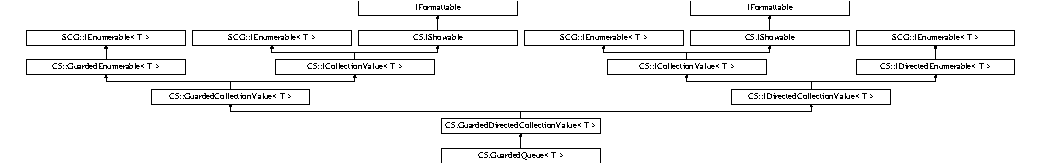
\includegraphics[height=2.178988cm]{class_c5_1_1_guarded_directed_collection_value}
\end{center}
\end{figure}
\subsection*{Public Member Functions}
\begin{DoxyCompactItemize}
\item 
\hyperlink{class_c5_1_1_guarded_directed_collection_value_ad940eb94010d945eae313b9375dd2df6}{Guarded\+Directed\+Collection\+Value} (\hyperlink{interface_c5_1_1_i_directed_collection_value}{I\+Directed\+Collection\+Value}$<$ T $>$ directedcollection)
\begin{DoxyCompactList}\small\item\em Wrap a directed collection in a read-\/only wrapper \end{DoxyCompactList}\item 
virtual \hyperlink{interface_c5_1_1_i_directed_collection_value}{I\+Directed\+Collection\+Value}$<$ T $>$ \hyperlink{class_c5_1_1_guarded_directed_collection_value_a14e2ad2eb0afbaf5e1ad2e970db81a5b}{Backwards} ()
\begin{DoxyCompactList}\small\item\em Get a collection that enumerates the wrapped collection in the opposite direction \end{DoxyCompactList}\item 
virtual bool \hyperlink{class_c5_1_1_guarded_directed_collection_value_a755cdf8f197ed79d7616a2b2527d718d}{Find\+Last} (Func$<$ T, bool $>$ predicate, out T item)
\end{DoxyCompactItemize}
\subsection*{Properties}
\begin{DoxyCompactItemize}
\item 
\hyperlink{namespace_c5_aad282676794e49130eb8caed289395f8}{Enumeration\+Direction} \hyperlink{class_c5_1_1_guarded_directed_collection_value_a5062645b3c4338673fa971a7abe5b1e2}{Direction}\hspace{0.3cm}{\ttfamily  \mbox{[}get\mbox{]}}
\end{DoxyCompactItemize}
\subsection*{Additional Inherited Members}


\subsection{Detailed Description}
A read-\/only wrapper for a directed collection 

{\itshape This is mainly interesting as a base of other guard classes} 

\subsection{Constructor \& Destructor Documentation}
\hypertarget{class_c5_1_1_guarded_directed_collection_value_ad940eb94010d945eae313b9375dd2df6}{}\index{C5\+::\+Guarded\+Directed\+Collection\+Value@{C5\+::\+Guarded\+Directed\+Collection\+Value}!Guarded\+Directed\+Collection\+Value@{Guarded\+Directed\+Collection\+Value}}
\index{Guarded\+Directed\+Collection\+Value@{Guarded\+Directed\+Collection\+Value}!C5\+::\+Guarded\+Directed\+Collection\+Value@{C5\+::\+Guarded\+Directed\+Collection\+Value}}
\subsubsection[{Guarded\+Directed\+Collection\+Value(\+I\+Directed\+Collection\+Value$<$ T $>$ directedcollection)}]{\setlength{\rightskip}{0pt plus 5cm}{\bf C5.\+Guarded\+Directed\+Collection\+Value}$<$ T $>$.{\bf Guarded\+Directed\+Collection\+Value} (
\begin{DoxyParamCaption}
\item[{{\bf I\+Directed\+Collection\+Value}$<$ T $>$}]{directedcollection}
\end{DoxyParamCaption}
)}\label{class_c5_1_1_guarded_directed_collection_value_ad940eb94010d945eae313b9375dd2df6}


Wrap a directed collection in a read-\/only wrapper 


\begin{DoxyParams}{Parameters}
{\em directedcollection} & the collection to wrap\\
\hline
\end{DoxyParams}


\subsection{Member Function Documentation}
\hypertarget{class_c5_1_1_guarded_directed_collection_value_a14e2ad2eb0afbaf5e1ad2e970db81a5b}{}\index{C5\+::\+Guarded\+Directed\+Collection\+Value@{C5\+::\+Guarded\+Directed\+Collection\+Value}!Backwards@{Backwards}}
\index{Backwards@{Backwards}!C5\+::\+Guarded\+Directed\+Collection\+Value@{C5\+::\+Guarded\+Directed\+Collection\+Value}}
\subsubsection[{Backwards()}]{\setlength{\rightskip}{0pt plus 5cm}virtual {\bf I\+Directed\+Collection\+Value}$<$T$>$ {\bf C5.\+Guarded\+Directed\+Collection\+Value}$<$ T $>$.Backwards (
\begin{DoxyParamCaption}
{}
\end{DoxyParamCaption}
)\hspace{0.3cm}{\ttfamily [virtual]}}\label{class_c5_1_1_guarded_directed_collection_value_a14e2ad2eb0afbaf5e1ad2e970db81a5b}


Get a collection that enumerates the wrapped collection in the opposite direction 

\begin{DoxyReturn}{Returns}
The mirrored collection
\end{DoxyReturn}


Implements \hyperlink{interface_c5_1_1_i_directed_collection_value_ae5665ed396ea2801266c4b2bfb3dae41}{C5.\+I\+Directed\+Collection\+Value$<$ T $>$}.

\hypertarget{class_c5_1_1_guarded_directed_collection_value_a755cdf8f197ed79d7616a2b2527d718d}{}\index{C5\+::\+Guarded\+Directed\+Collection\+Value@{C5\+::\+Guarded\+Directed\+Collection\+Value}!Find\+Last@{Find\+Last}}
\index{Find\+Last@{Find\+Last}!C5\+::\+Guarded\+Directed\+Collection\+Value@{C5\+::\+Guarded\+Directed\+Collection\+Value}}
\subsubsection[{Find\+Last(\+Func$<$ T, bool $>$ predicate, out T item)}]{\setlength{\rightskip}{0pt plus 5cm}virtual bool {\bf C5.\+Guarded\+Directed\+Collection\+Value}$<$ T $>$.Find\+Last (
\begin{DoxyParamCaption}
\item[{Func$<$ T, bool $>$}]{predicate, }
\item[{out T}]{item}
\end{DoxyParamCaption}
)\hspace{0.3cm}{\ttfamily [virtual]}}\label{class_c5_1_1_guarded_directed_collection_value_a755cdf8f197ed79d7616a2b2527d718d}





\begin{DoxyParams}{Parameters}
{\em predicate} & \\
\hline
{\em item} & \\
\hline
\end{DoxyParams}
\begin{DoxyReturn}{Returns}

\end{DoxyReturn}


Implements \hyperlink{interface_c5_1_1_i_directed_collection_value_a93725b1f694e0d1cf5827e481ea467b7}{C5.\+I\+Directed\+Collection\+Value$<$ T $>$}.



\subsection{Property Documentation}
\hypertarget{class_c5_1_1_guarded_directed_collection_value_a5062645b3c4338673fa971a7abe5b1e2}{}\index{C5\+::\+Guarded\+Directed\+Collection\+Value@{C5\+::\+Guarded\+Directed\+Collection\+Value}!Direction@{Direction}}
\index{Direction@{Direction}!C5\+::\+Guarded\+Directed\+Collection\+Value@{C5\+::\+Guarded\+Directed\+Collection\+Value}}
\subsubsection[{Direction}]{\setlength{\rightskip}{0pt plus 5cm}{\bf Enumeration\+Direction} {\bf C5.\+Guarded\+Directed\+Collection\+Value}$<$ T $>$.Direction\hspace{0.3cm}{\ttfamily [get]}}\label{class_c5_1_1_guarded_directed_collection_value_a5062645b3c4338673fa971a7abe5b1e2}




{\ttfamily Forwards} if same, else {\ttfamily Backwards} 

The enumeration direction relative to the original collection.

The documentation for this class was generated from the following file\+:\begin{DoxyCompactItemize}
\item 
C\+:/\+Users/rasmusl/\+Source/\+Repos/\+C5/\+C5/\hyperlink{_wrappers_8cs}{Wrappers.\+cs}\end{DoxyCompactItemize}

\hypertarget{class_c5_1_1_guarded_directed_enumerable}{}\section{C5.\+Guarded\+Directed\+Enumerable$<$ T $>$ Class Template Reference}
\label{class_c5_1_1_guarded_directed_enumerable}\index{C5.\+Guarded\+Directed\+Enumerable$<$ T $>$@{C5.\+Guarded\+Directed\+Enumerable$<$ T $>$}}


A read-\/only wrapper for a generic directed enumerable  


Inheritance diagram for C5.\+Guarded\+Directed\+Enumerable$<$ T $>$\+:\begin{figure}[H]
\begin{center}
\leavevmode
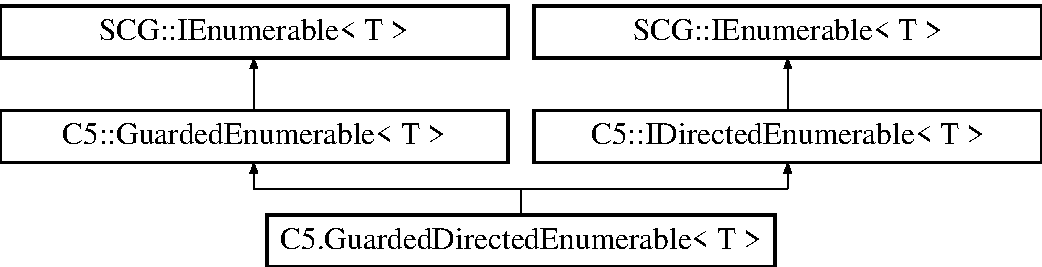
\includegraphics[height=3.000000cm]{class_c5_1_1_guarded_directed_enumerable}
\end{center}
\end{figure}
\subsection*{Public Member Functions}
\begin{DoxyCompactItemize}
\item 
\hyperlink{class_c5_1_1_guarded_directed_enumerable_a2df0b6305f4f08aefe05e0e55887144c}{Guarded\+Directed\+Enumerable} (\hyperlink{interface_c5_1_1_i_directed_enumerable}{I\+Directed\+Enumerable}$<$ T $>$ directedenumerable)
\begin{DoxyCompactList}\small\item\em Wrap a directed enumerable in a read-\/only wrapper \end{DoxyCompactList}\item 
\hyperlink{interface_c5_1_1_i_directed_enumerable}{I\+Directed\+Enumerable}$<$ T $>$ \hyperlink{class_c5_1_1_guarded_directed_enumerable_a858ca7e55fc0cf083c967e31d9beb8eb}{Backwards} ()
\begin{DoxyCompactList}\small\item\em Get a enumerable that enumerates the wrapped collection in the opposite direction \end{DoxyCompactList}\end{DoxyCompactItemize}
\subsection*{Properties}
\begin{DoxyCompactItemize}
\item 
\hyperlink{namespace_c5_aad282676794e49130eb8caed289395f8}{Enumeration\+Direction} \hyperlink{class_c5_1_1_guarded_directed_enumerable_ad485f49a2e4938d130d0028d38d1319f}{Direction}\hspace{0.3cm}{\ttfamily  \mbox{[}get\mbox{]}}
\end{DoxyCompactItemize}


\subsection{Detailed Description}
A read-\/only wrapper for a generic directed enumerable 

{\itshape This is mainly interesting as a base of other guard classes} 

\subsection{Constructor \& Destructor Documentation}
\hypertarget{class_c5_1_1_guarded_directed_enumerable_a2df0b6305f4f08aefe05e0e55887144c}{}\index{C5\+::\+Guarded\+Directed\+Enumerable@{C5\+::\+Guarded\+Directed\+Enumerable}!Guarded\+Directed\+Enumerable@{Guarded\+Directed\+Enumerable}}
\index{Guarded\+Directed\+Enumerable@{Guarded\+Directed\+Enumerable}!C5\+::\+Guarded\+Directed\+Enumerable@{C5\+::\+Guarded\+Directed\+Enumerable}}
\subsubsection[{Guarded\+Directed\+Enumerable(\+I\+Directed\+Enumerable$<$ T $>$ directedenumerable)}]{\setlength{\rightskip}{0pt plus 5cm}{\bf C5.\+Guarded\+Directed\+Enumerable}$<$ T $>$.{\bf Guarded\+Directed\+Enumerable} (
\begin{DoxyParamCaption}
\item[{{\bf I\+Directed\+Enumerable}$<$ T $>$}]{directedenumerable}
\end{DoxyParamCaption}
)}\label{class_c5_1_1_guarded_directed_enumerable_a2df0b6305f4f08aefe05e0e55887144c}


Wrap a directed enumerable in a read-\/only wrapper 


\begin{DoxyParams}{Parameters}
{\em directedenumerable} & the collection to wrap\\
\hline
\end{DoxyParams}


\subsection{Member Function Documentation}
\hypertarget{class_c5_1_1_guarded_directed_enumerable_a858ca7e55fc0cf083c967e31d9beb8eb}{}\index{C5\+::\+Guarded\+Directed\+Enumerable@{C5\+::\+Guarded\+Directed\+Enumerable}!Backwards@{Backwards}}
\index{Backwards@{Backwards}!C5\+::\+Guarded\+Directed\+Enumerable@{C5\+::\+Guarded\+Directed\+Enumerable}}
\subsubsection[{Backwards()}]{\setlength{\rightskip}{0pt plus 5cm}{\bf I\+Directed\+Enumerable}$<$T$>$ {\bf C5.\+Guarded\+Directed\+Enumerable}$<$ T $>$.Backwards (
\begin{DoxyParamCaption}
{}
\end{DoxyParamCaption}
)}\label{class_c5_1_1_guarded_directed_enumerable_a858ca7e55fc0cf083c967e31d9beb8eb}


Get a enumerable that enumerates the wrapped collection in the opposite direction 

\begin{DoxyReturn}{Returns}
The mirrored enumerable
\end{DoxyReturn}


Implements \hyperlink{interface_c5_1_1_i_directed_enumerable_a826d9e7f29272dea7ebd48a38757df9e}{C5.\+I\+Directed\+Enumerable$<$ T $>$}.



\subsection{Property Documentation}
\hypertarget{class_c5_1_1_guarded_directed_enumerable_ad485f49a2e4938d130d0028d38d1319f}{}\index{C5\+::\+Guarded\+Directed\+Enumerable@{C5\+::\+Guarded\+Directed\+Enumerable}!Direction@{Direction}}
\index{Direction@{Direction}!C5\+::\+Guarded\+Directed\+Enumerable@{C5\+::\+Guarded\+Directed\+Enumerable}}
\subsubsection[{Direction}]{\setlength{\rightskip}{0pt plus 5cm}{\bf Enumeration\+Direction} {\bf C5.\+Guarded\+Directed\+Enumerable}$<$ T $>$.Direction\hspace{0.3cm}{\ttfamily [get]}}\label{class_c5_1_1_guarded_directed_enumerable_ad485f49a2e4938d130d0028d38d1319f}




{\ttfamily Forwards} if same, else {\ttfamily Backwards} 

The enumeration direction relative to the original collection.

The documentation for this class was generated from the following file\+:\begin{DoxyCompactItemize}
\item 
C\+:/\+Users/rasmusl/\+Source/\+Repos/\+C5/\+C5/\hyperlink{_wrappers_8cs}{Wrappers.\+cs}\end{DoxyCompactItemize}

\hypertarget{class_c5_1_1_guarded_enumerable}{}\section{C5.\+Guarded\+Enumerable$<$ T $>$ Class Template Reference}
\label{class_c5_1_1_guarded_enumerable}\index{C5.\+Guarded\+Enumerable$<$ T $>$@{C5.\+Guarded\+Enumerable$<$ T $>$}}


A read-\/only wrapper class for a generic enumerable  


Inheritance diagram for C5.\+Guarded\+Enumerable$<$ T $>$\+:\begin{figure}[H]
\begin{center}
\leavevmode
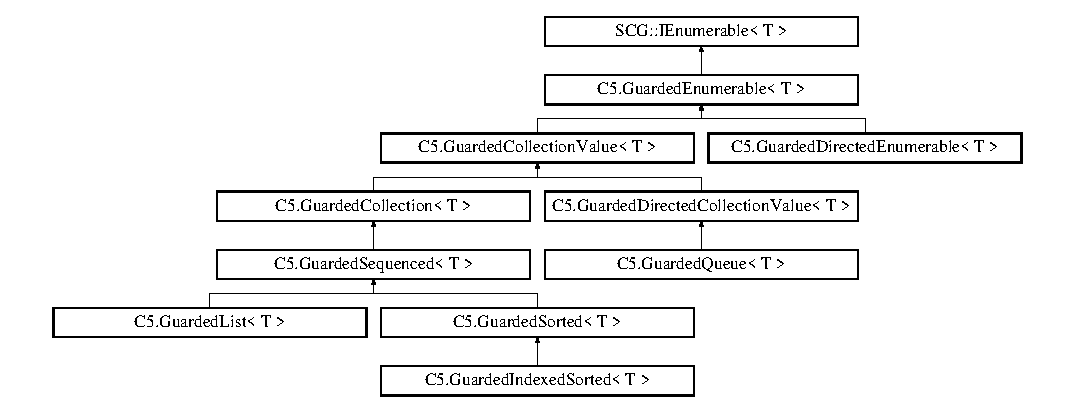
\includegraphics[height=5.084306cm]{class_c5_1_1_guarded_enumerable}
\end{center}
\end{figure}
\subsection*{Public Member Functions}
\begin{DoxyCompactItemize}
\item 
\hyperlink{class_c5_1_1_guarded_enumerable_acfdc32a8f8896ca793e93a12c863f58b}{Guarded\+Enumerable} (S\+C\+G.\+I\+Enumerable$<$ T $>$ enumerable)
\begin{DoxyCompactList}\small\item\em Wrap an enumerable in a read-\/only wrapper \end{DoxyCompactList}\item 
S\+C\+G.\+I\+Enumerator$<$ T $>$ \hyperlink{class_c5_1_1_guarded_enumerable_aab3a7dc7eeb5ab3b64764333037ff119}{Get\+Enumerator} ()
\begin{DoxyCompactList}\small\item\em Get an enumerator from the wrapped enumerable \end{DoxyCompactList}\end{DoxyCompactItemize}


\subsection{Detailed Description}
A read-\/only wrapper class for a generic enumerable 

{\itshape This is mainly interesting as a base of other guard classes} 

\subsection{Constructor \& Destructor Documentation}
\hypertarget{class_c5_1_1_guarded_enumerable_acfdc32a8f8896ca793e93a12c863f58b}{}\index{C5\+::\+Guarded\+Enumerable@{C5\+::\+Guarded\+Enumerable}!Guarded\+Enumerable@{Guarded\+Enumerable}}
\index{Guarded\+Enumerable@{Guarded\+Enumerable}!C5\+::\+Guarded\+Enumerable@{C5\+::\+Guarded\+Enumerable}}
\subsubsection[{Guarded\+Enumerable(\+S\+C\+G.\+I\+Enumerable$<$ T $>$ enumerable)}]{\setlength{\rightskip}{0pt plus 5cm}{\bf C5.\+Guarded\+Enumerable}$<$ T $>$.{\bf Guarded\+Enumerable} (
\begin{DoxyParamCaption}
\item[{S\+C\+G.\+I\+Enumerable$<$ T $>$}]{enumerable}
\end{DoxyParamCaption}
)}\label{class_c5_1_1_guarded_enumerable_acfdc32a8f8896ca793e93a12c863f58b}


Wrap an enumerable in a read-\/only wrapper 


\begin{DoxyParams}{Parameters}
{\em enumerable} & The enumerable to wrap\\
\hline
\end{DoxyParams}


\subsection{Member Function Documentation}
\hypertarget{class_c5_1_1_guarded_enumerable_aab3a7dc7eeb5ab3b64764333037ff119}{}\index{C5\+::\+Guarded\+Enumerable@{C5\+::\+Guarded\+Enumerable}!Get\+Enumerator@{Get\+Enumerator}}
\index{Get\+Enumerator@{Get\+Enumerator}!C5\+::\+Guarded\+Enumerable@{C5\+::\+Guarded\+Enumerable}}
\subsubsection[{Get\+Enumerator()}]{\setlength{\rightskip}{0pt plus 5cm}S\+C\+G.\+I\+Enumerator$<$T$>$ {\bf C5.\+Guarded\+Enumerable}$<$ T $>$.Get\+Enumerator (
\begin{DoxyParamCaption}
{}
\end{DoxyParamCaption}
)}\label{class_c5_1_1_guarded_enumerable_aab3a7dc7eeb5ab3b64764333037ff119}


Get an enumerator from the wrapped enumerable 

\begin{DoxyReturn}{Returns}
The enumerator (itself wrapped)
\end{DoxyReturn}


The documentation for this class was generated from the following file\+:\begin{DoxyCompactItemize}
\item 
C\+:/\+Users/rasmusl/\+Source/\+Repos/\+C5/\+C5/\hyperlink{_wrappers_8cs}{Wrappers.\+cs}\end{DoxyCompactItemize}

\hypertarget{class_c5_1_1_guarded_enumerator}{}\section{C5.\+Guarded\+Enumerator$<$ T $>$ Class Template Reference}
\label{class_c5_1_1_guarded_enumerator}\index{C5.\+Guarded\+Enumerator$<$ T $>$@{C5.\+Guarded\+Enumerator$<$ T $>$}}


A read-\/only wrapper class for a generic enumerator  


Inheritance diagram for C5.\+Guarded\+Enumerator$<$ T $>$\+:\begin{figure}[H]
\begin{center}
\leavevmode
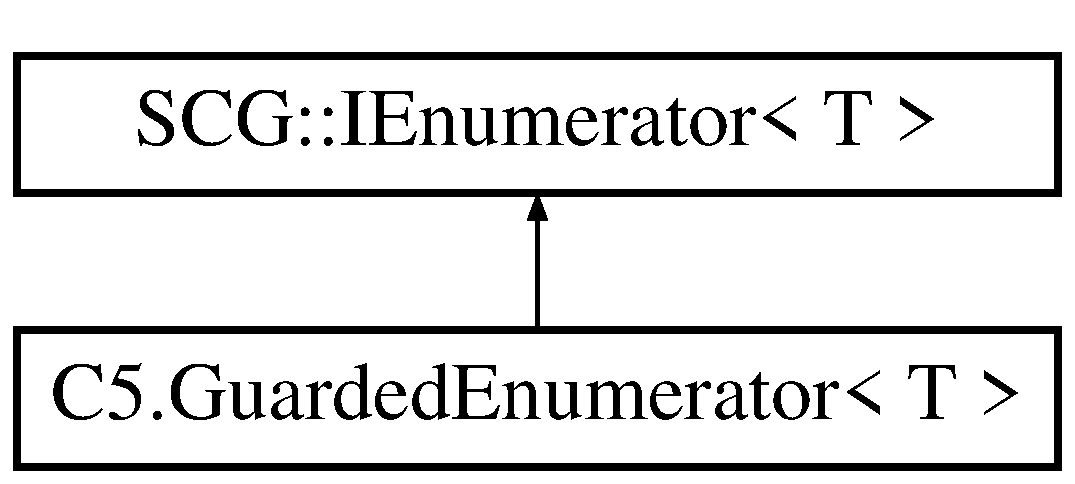
\includegraphics[height=2.000000cm]{class_c5_1_1_guarded_enumerator}
\end{center}
\end{figure}
\subsection*{Public Member Functions}
\begin{DoxyCompactItemize}
\item 
\hyperlink{class_c5_1_1_guarded_enumerator_a26e05b27464a89352253e1a683c0750a}{Guarded\+Enumerator} (S\+C\+G.\+I\+Enumerator$<$ T $>$ enumerator)
\begin{DoxyCompactList}\small\item\em Create a wrapper around a generic enumerator \end{DoxyCompactList}\item 
bool \hyperlink{class_c5_1_1_guarded_enumerator_a2fad3f14e61f9fa762730de1ab42d68d}{Move\+Next} ()
\begin{DoxyCompactList}\small\item\em Move wrapped enumerator to next item, or the first item if this is the first call to Move\+Next. \end{DoxyCompactList}\item 
void \hyperlink{class_c5_1_1_guarded_enumerator_a2733fc78a530e8212dc160b9a6aa395f}{Dispose} ()
\begin{DoxyCompactList}\small\item\em Dispose wrapped enumerator. \end{DoxyCompactList}\end{DoxyCompactItemize}
\subsection*{Properties}
\begin{DoxyCompactItemize}
\item 
T \hyperlink{class_c5_1_1_guarded_enumerator_af13904801a980feda3b2d6a4ec03db2c}{Current}\hspace{0.3cm}{\ttfamily  \mbox{[}get\mbox{]}}
\begin{DoxyCompactList}\small\item\em Undefined if enumerator is not valid (Move\+Next hash been called returning true) \end{DoxyCompactList}\end{DoxyCompactItemize}


\subsection{Detailed Description}
A read-\/only wrapper class for a generic enumerator 



\subsection{Constructor \& Destructor Documentation}
\hypertarget{class_c5_1_1_guarded_enumerator_a26e05b27464a89352253e1a683c0750a}{}\index{C5\+::\+Guarded\+Enumerator@{C5\+::\+Guarded\+Enumerator}!Guarded\+Enumerator@{Guarded\+Enumerator}}
\index{Guarded\+Enumerator@{Guarded\+Enumerator}!C5\+::\+Guarded\+Enumerator@{C5\+::\+Guarded\+Enumerator}}
\subsubsection[{Guarded\+Enumerator(\+S\+C\+G.\+I\+Enumerator$<$ T $>$ enumerator)}]{\setlength{\rightskip}{0pt plus 5cm}{\bf C5.\+Guarded\+Enumerator}$<$ T $>$.{\bf Guarded\+Enumerator} (
\begin{DoxyParamCaption}
\item[{S\+C\+G.\+I\+Enumerator$<$ T $>$}]{enumerator}
\end{DoxyParamCaption}
)}\label{class_c5_1_1_guarded_enumerator_a26e05b27464a89352253e1a683c0750a}


Create a wrapper around a generic enumerator 


\begin{DoxyParams}{Parameters}
{\em enumerator} & The enumerator to wrap\\
\hline
\end{DoxyParams}


\subsection{Member Function Documentation}
\hypertarget{class_c5_1_1_guarded_enumerator_a2733fc78a530e8212dc160b9a6aa395f}{}\index{C5\+::\+Guarded\+Enumerator@{C5\+::\+Guarded\+Enumerator}!Dispose@{Dispose}}
\index{Dispose@{Dispose}!C5\+::\+Guarded\+Enumerator@{C5\+::\+Guarded\+Enumerator}}
\subsubsection[{Dispose()}]{\setlength{\rightskip}{0pt plus 5cm}void {\bf C5.\+Guarded\+Enumerator}$<$ T $>$.Dispose (
\begin{DoxyParamCaption}
{}
\end{DoxyParamCaption}
)}\label{class_c5_1_1_guarded_enumerator_a2733fc78a530e8212dc160b9a6aa395f}


Dispose wrapped enumerator. 

\hypertarget{class_c5_1_1_guarded_enumerator_a2fad3f14e61f9fa762730de1ab42d68d}{}\index{C5\+::\+Guarded\+Enumerator@{C5\+::\+Guarded\+Enumerator}!Move\+Next@{Move\+Next}}
\index{Move\+Next@{Move\+Next}!C5\+::\+Guarded\+Enumerator@{C5\+::\+Guarded\+Enumerator}}
\subsubsection[{Move\+Next()}]{\setlength{\rightskip}{0pt plus 5cm}bool {\bf C5.\+Guarded\+Enumerator}$<$ T $>$.Move\+Next (
\begin{DoxyParamCaption}
{}
\end{DoxyParamCaption}
)}\label{class_c5_1_1_guarded_enumerator_a2fad3f14e61f9fa762730de1ab42d68d}


Move wrapped enumerator to next item, or the first item if this is the first call to Move\+Next. 

\begin{DoxyReturn}{Returns}
True if enumerator is valid now
\end{DoxyReturn}


\subsection{Property Documentation}
\hypertarget{class_c5_1_1_guarded_enumerator_af13904801a980feda3b2d6a4ec03db2c}{}\index{C5\+::\+Guarded\+Enumerator@{C5\+::\+Guarded\+Enumerator}!Current@{Current}}
\index{Current@{Current}!C5\+::\+Guarded\+Enumerator@{C5\+::\+Guarded\+Enumerator}}
\subsubsection[{Current}]{\setlength{\rightskip}{0pt plus 5cm}T {\bf C5.\+Guarded\+Enumerator}$<$ T $>$.Current\hspace{0.3cm}{\ttfamily [get]}}\label{class_c5_1_1_guarded_enumerator_af13904801a980feda3b2d6a4ec03db2c}


Undefined if enumerator is not valid (Move\+Next hash been called returning true) 

The current item of the wrapped enumerator.

The documentation for this class was generated from the following file\+:\begin{DoxyCompactItemize}
\item 
C\+:/\+Users/rasmusl/\+Source/\+Repos/\+C5/\+C5/\hyperlink{_wrappers_8cs}{Wrappers.\+cs}\end{DoxyCompactItemize}

\hypertarget{class_c5_1_1_guarded_indexed_sorted}{}\section{C5.\+Guarded\+Indexed\+Sorted$<$ T $>$ Class Template Reference}
\label{class_c5_1_1_guarded_indexed_sorted}\index{C5.\+Guarded\+Indexed\+Sorted$<$ T $>$@{C5.\+Guarded\+Indexed\+Sorted$<$ T $>$}}


Read-\/only wrapper for indexed sorted collections  


Inheritance diagram for C5.\+Guarded\+Indexed\+Sorted$<$ T $>$\+:\begin{figure}[H]
\begin{center}
\leavevmode
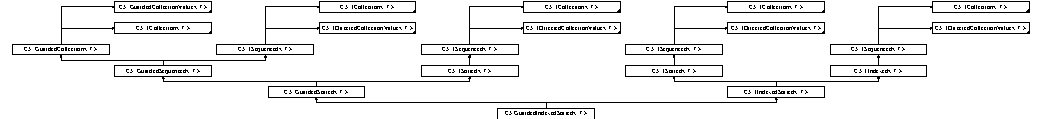
\includegraphics[height=1.577465cm]{class_c5_1_1_guarded_indexed_sorted}
\end{center}
\end{figure}
\subsection*{Public Member Functions}
\begin{DoxyCompactItemize}
\item 
\hyperlink{class_c5_1_1_guarded_indexed_sorted_ae5ded6570af9716bb93a42e5dea55656}{Guarded\+Indexed\+Sorted} (\hyperlink{interface_c5_1_1_i_indexed_sorted}{I\+Indexed\+Sorted}$<$ T $>$ list)
\begin{DoxyCompactList}\small\item\em Wrap an indexed sorted collection in a read-\/only wrapper \end{DoxyCompactList}\item 
new \hyperlink{interface_c5_1_1_i_directed_collection_value}{I\+Directed\+Collection\+Value}$<$ T $>$ \hyperlink{class_c5_1_1_guarded_indexed_sorted_a4234ea1cd38561949156953beb98a19e}{Range\+From} (T bot)
\begin{DoxyCompactList}\small\item\em Get the specified range from the wrapped collection. (The current implementation erroneously does not wrap the result.) \end{DoxyCompactList}\item 
new \hyperlink{interface_c5_1_1_i_directed_collection_value}{I\+Directed\+Collection\+Value}$<$ T $>$ \hyperlink{class_c5_1_1_guarded_indexed_sorted_a039a34453e6451fce027438afed623b0}{Range\+From\+To} (T bot, T top)
\begin{DoxyCompactList}\small\item\em Get the specified range from the wrapped collection. (The current implementation erroneously does not wrap the result.) \end{DoxyCompactList}\item 
new \hyperlink{interface_c5_1_1_i_directed_collection_value}{I\+Directed\+Collection\+Value}$<$ T $>$ \hyperlink{class_c5_1_1_guarded_indexed_sorted_a99cbd7079a015107d98567b63398aa77}{Range\+To} (T top)
\begin{DoxyCompactList}\small\item\em Get the specified range from the wrapped collection. (The current implementation erroneously does not wrap the result.) \end{DoxyCompactList}\item 
int \hyperlink{class_c5_1_1_guarded_indexed_sorted_a8cf3d09d8c435ac0200efc34561e1a86}{Count\+From} (T bot)
\begin{DoxyCompactList}\small\item\em Report the number of items in the specified range of the wrapped collection \end{DoxyCompactList}\item 
int \hyperlink{class_c5_1_1_guarded_indexed_sorted_af8a01e371525dfae61ddc323e16e1f9e}{Count\+From\+To} (T bot, T top)
\begin{DoxyCompactList}\small\item\em Report the number of items in the specified range of the wrapped collection \end{DoxyCompactList}\item 
int \hyperlink{class_c5_1_1_guarded_indexed_sorted_abfdc8d50b6ea0bf7493fbcf77c4ae19a}{Count\+To} (T top)
\begin{DoxyCompactList}\small\item\em Report the number of items in the specified range of the wrapped collection \end{DoxyCompactList}\item 
\hyperlink{interface_c5_1_1_i_indexed_sorted}{I\+Indexed\+Sorted}$<$ T $>$ \hyperlink{class_c5_1_1_guarded_indexed_sorted_ab5bc00909aa5b210f3de4f09e674d7b0}{Find\+All} (Func$<$ T, bool $>$ f)
\begin{DoxyCompactList}\small\item\em Run Find\+All on the wrapped collection with the indicated filter. The result will {\bfseries not} be read-\/only. \end{DoxyCompactList}\item 
\hyperlink{interface_c5_1_1_i_indexed_sorted}{I\+Indexed\+Sorted}$<$ V $>$ \hyperlink{class_c5_1_1_guarded_indexed_sorted_a9f01bb786e4abb2c27d3d38aedd47a70}{Map$<$ V $>$} (Func$<$ T, V $>$ m, S\+C\+G.\+I\+Comparer$<$ V $>$ c)
\begin{DoxyCompactList}\small\item\em Run Map on the wrapped collection with the indicated mapper. The result will {\bfseries not} be read-\/only. \end{DoxyCompactList}\item 
int \hyperlink{class_c5_1_1_guarded_indexed_sorted_aa13e57faa854dd70f28ac2dd8bb6f888}{Index\+Of} (T item)
\begin{DoxyCompactList}\small\item\em Find the (first) index of an item in the wrapped collection \end{DoxyCompactList}\item 
int \hyperlink{class_c5_1_1_guarded_indexed_sorted_a782d9e939a68f246af69adba83584164}{Last\+Index\+Of} (T item)
\begin{DoxyCompactList}\small\item\em Find the last index of an item in the wrapped collection \end{DoxyCompactList}\item 
T \hyperlink{class_c5_1_1_guarded_indexed_sorted_a0e84a6bb3bf610cdf68aa2583dc78155}{Remove\+At} (int i)
\item 
void \hyperlink{class_c5_1_1_guarded_indexed_sorted_a2c43f17a32750da03b1aa64a6300a091}{Remove\+Interval} (int start, int count)
\end{DoxyCompactItemize}
\subsection*{Properties}
\begin{DoxyCompactItemize}
\item 
T \hyperlink{class_c5_1_1_guarded_indexed_sorted_a56e09512c3d2bfccb720141d7239cdc5}{this\mbox{[}int i\mbox{]}}\hspace{0.3cm}{\ttfamily  \mbox{[}get\mbox{]}}
\item 
virtual \hyperlink{namespace_c5_a615ba88dcdaa8d5a3c5f833a73d7fad6}{Speed} \hyperlink{class_c5_1_1_guarded_indexed_sorted_a57f771060cc1af22826097d4f7fa002f}{Indexing\+Speed}\hspace{0.3cm}{\ttfamily  \mbox{[}get\mbox{]}}
\item 
\hyperlink{interface_c5_1_1_i_directed_collection_value}{I\+Directed\+Collection\+Value}$<$ T $>$ \hyperlink{class_c5_1_1_guarded_indexed_sorted_a5c5994179a814f8eb2d75007fe5aa628}{this\mbox{[}int start, int end\mbox{]}}\hspace{0.3cm}{\ttfamily  \mbox{[}get\mbox{]}}
\end{DoxyCompactItemize}
\subsection*{Additional Inherited Members}


\subsection{Detailed Description}
Read-\/only wrapper for indexed sorted collections 

{\itshape Suitable for wrapping \hyperlink{class_c5_1_1_tree_set}{Tree\+Set}, \hyperlink{class_c5_1_1_tree_bag}{Tree\+Bag} and \hyperlink{class_c5_1_1_sorted_array}{Sorted\+Array}} 

\subsection{Constructor \& Destructor Documentation}
\hypertarget{class_c5_1_1_guarded_indexed_sorted_ae5ded6570af9716bb93a42e5dea55656}{}\index{C5\+::\+Guarded\+Indexed\+Sorted@{C5\+::\+Guarded\+Indexed\+Sorted}!Guarded\+Indexed\+Sorted@{Guarded\+Indexed\+Sorted}}
\index{Guarded\+Indexed\+Sorted@{Guarded\+Indexed\+Sorted}!C5\+::\+Guarded\+Indexed\+Sorted@{C5\+::\+Guarded\+Indexed\+Sorted}}
\subsubsection[{Guarded\+Indexed\+Sorted(\+I\+Indexed\+Sorted$<$ T $>$ list)}]{\setlength{\rightskip}{0pt plus 5cm}{\bf C5.\+Guarded\+Indexed\+Sorted}$<$ T $>$.{\bf Guarded\+Indexed\+Sorted} (
\begin{DoxyParamCaption}
\item[{{\bf I\+Indexed\+Sorted}$<$ T $>$}]{list}
\end{DoxyParamCaption}
)}\label{class_c5_1_1_guarded_indexed_sorted_ae5ded6570af9716bb93a42e5dea55656}


Wrap an indexed sorted collection in a read-\/only wrapper 


\begin{DoxyParams}{Parameters}
{\em list} & the indexed sorted collection\\
\hline
\end{DoxyParams}


\subsection{Member Function Documentation}
\hypertarget{class_c5_1_1_guarded_indexed_sorted_a8cf3d09d8c435ac0200efc34561e1a86}{}\index{C5\+::\+Guarded\+Indexed\+Sorted@{C5\+::\+Guarded\+Indexed\+Sorted}!Count\+From@{Count\+From}}
\index{Count\+From@{Count\+From}!C5\+::\+Guarded\+Indexed\+Sorted@{C5\+::\+Guarded\+Indexed\+Sorted}}
\subsubsection[{Count\+From(\+T bot)}]{\setlength{\rightskip}{0pt plus 5cm}int {\bf C5.\+Guarded\+Indexed\+Sorted}$<$ T $>$.Count\+From (
\begin{DoxyParamCaption}
\item[{T}]{bot}
\end{DoxyParamCaption}
)}\label{class_c5_1_1_guarded_indexed_sorted_a8cf3d09d8c435ac0200efc34561e1a86}


Report the number of items in the specified range of the wrapped collection 


\begin{DoxyParams}{Parameters}
{\em bot} & \\
\hline
\end{DoxyParams}
\begin{DoxyReturn}{Returns}

\end{DoxyReturn}


Implements \hyperlink{interface_c5_1_1_i_indexed_sorted_afec472803ce8298d60dfc5dfb2f8f925}{C5.\+I\+Indexed\+Sorted$<$ T $>$}.

\hypertarget{class_c5_1_1_guarded_indexed_sorted_af8a01e371525dfae61ddc323e16e1f9e}{}\index{C5\+::\+Guarded\+Indexed\+Sorted@{C5\+::\+Guarded\+Indexed\+Sorted}!Count\+From\+To@{Count\+From\+To}}
\index{Count\+From\+To@{Count\+From\+To}!C5\+::\+Guarded\+Indexed\+Sorted@{C5\+::\+Guarded\+Indexed\+Sorted}}
\subsubsection[{Count\+From\+To(\+T bot, T top)}]{\setlength{\rightskip}{0pt plus 5cm}int {\bf C5.\+Guarded\+Indexed\+Sorted}$<$ T $>$.Count\+From\+To (
\begin{DoxyParamCaption}
\item[{T}]{bot, }
\item[{T}]{top}
\end{DoxyParamCaption}
)}\label{class_c5_1_1_guarded_indexed_sorted_af8a01e371525dfae61ddc323e16e1f9e}


Report the number of items in the specified range of the wrapped collection 


\begin{DoxyParams}{Parameters}
{\em bot} & \\
\hline
{\em top} & \\
\hline
\end{DoxyParams}
\begin{DoxyReturn}{Returns}

\end{DoxyReturn}


Implements \hyperlink{interface_c5_1_1_i_indexed_sorted_a6b8dd3c5325621b9a81a7e5167328773}{C5.\+I\+Indexed\+Sorted$<$ T $>$}.

\hypertarget{class_c5_1_1_guarded_indexed_sorted_abfdc8d50b6ea0bf7493fbcf77c4ae19a}{}\index{C5\+::\+Guarded\+Indexed\+Sorted@{C5\+::\+Guarded\+Indexed\+Sorted}!Count\+To@{Count\+To}}
\index{Count\+To@{Count\+To}!C5\+::\+Guarded\+Indexed\+Sorted@{C5\+::\+Guarded\+Indexed\+Sorted}}
\subsubsection[{Count\+To(\+T top)}]{\setlength{\rightskip}{0pt plus 5cm}int {\bf C5.\+Guarded\+Indexed\+Sorted}$<$ T $>$.Count\+To (
\begin{DoxyParamCaption}
\item[{T}]{top}
\end{DoxyParamCaption}
)}\label{class_c5_1_1_guarded_indexed_sorted_abfdc8d50b6ea0bf7493fbcf77c4ae19a}


Report the number of items in the specified range of the wrapped collection 


\begin{DoxyParams}{Parameters}
{\em top} & \\
\hline
\end{DoxyParams}
\begin{DoxyReturn}{Returns}

\end{DoxyReturn}


Implements \hyperlink{interface_c5_1_1_i_indexed_sorted_ae69946df07200b99fa1336681223680a}{C5.\+I\+Indexed\+Sorted$<$ T $>$}.

\hypertarget{class_c5_1_1_guarded_indexed_sorted_ab5bc00909aa5b210f3de4f09e674d7b0}{}\index{C5\+::\+Guarded\+Indexed\+Sorted@{C5\+::\+Guarded\+Indexed\+Sorted}!Find\+All@{Find\+All}}
\index{Find\+All@{Find\+All}!C5\+::\+Guarded\+Indexed\+Sorted@{C5\+::\+Guarded\+Indexed\+Sorted}}
\subsubsection[{Find\+All(\+Func$<$ T, bool $>$ f)}]{\setlength{\rightskip}{0pt plus 5cm}{\bf I\+Indexed\+Sorted}$<$T$>$ {\bf C5.\+Guarded\+Indexed\+Sorted}$<$ T $>$.Find\+All (
\begin{DoxyParamCaption}
\item[{Func$<$ T, bool $>$}]{f}
\end{DoxyParamCaption}
)}\label{class_c5_1_1_guarded_indexed_sorted_ab5bc00909aa5b210f3de4f09e674d7b0}


Run Find\+All on the wrapped collection with the indicated filter. The result will {\bfseries not} be read-\/only. 


\begin{DoxyParams}{Parameters}
{\em f} & \\
\hline
\end{DoxyParams}
\begin{DoxyReturn}{Returns}

\end{DoxyReturn}


Implements \hyperlink{interface_c5_1_1_i_indexed_sorted_a0919e5cb5b659d0de7c206a3c3bc033d}{C5.\+I\+Indexed\+Sorted$<$ T $>$}.

\hypertarget{class_c5_1_1_guarded_indexed_sorted_aa13e57faa854dd70f28ac2dd8bb6f888}{}\index{C5\+::\+Guarded\+Indexed\+Sorted@{C5\+::\+Guarded\+Indexed\+Sorted}!Index\+Of@{Index\+Of}}
\index{Index\+Of@{Index\+Of}!C5\+::\+Guarded\+Indexed\+Sorted@{C5\+::\+Guarded\+Indexed\+Sorted}}
\subsubsection[{Index\+Of(\+T item)}]{\setlength{\rightskip}{0pt plus 5cm}int {\bf C5.\+Guarded\+Indexed\+Sorted}$<$ T $>$.Index\+Of (
\begin{DoxyParamCaption}
\item[{T}]{item}
\end{DoxyParamCaption}
)}\label{class_c5_1_1_guarded_indexed_sorted_aa13e57faa854dd70f28ac2dd8bb6f888}


Find the (first) index of an item in the wrapped collection 


\begin{DoxyParams}{Parameters}
{\em item} & \\
\hline
\end{DoxyParams}
\begin{DoxyReturn}{Returns}

\end{DoxyReturn}


Implements \hyperlink{interface_c5_1_1_i_indexed_abad58598415e0383ddbc9275db69d92a}{C5.\+I\+Indexed$<$ T $>$}.

\hypertarget{class_c5_1_1_guarded_indexed_sorted_a782d9e939a68f246af69adba83584164}{}\index{C5\+::\+Guarded\+Indexed\+Sorted@{C5\+::\+Guarded\+Indexed\+Sorted}!Last\+Index\+Of@{Last\+Index\+Of}}
\index{Last\+Index\+Of@{Last\+Index\+Of}!C5\+::\+Guarded\+Indexed\+Sorted@{C5\+::\+Guarded\+Indexed\+Sorted}}
\subsubsection[{Last\+Index\+Of(\+T item)}]{\setlength{\rightskip}{0pt plus 5cm}int {\bf C5.\+Guarded\+Indexed\+Sorted}$<$ T $>$.Last\+Index\+Of (
\begin{DoxyParamCaption}
\item[{T}]{item}
\end{DoxyParamCaption}
)}\label{class_c5_1_1_guarded_indexed_sorted_a782d9e939a68f246af69adba83584164}


Find the last index of an item in the wrapped collection 


\begin{DoxyParams}{Parameters}
{\em item} & \\
\hline
\end{DoxyParams}
\begin{DoxyReturn}{Returns}

\end{DoxyReturn}


Implements \hyperlink{interface_c5_1_1_i_indexed_a50f274e0f7b4cd2e54db4cb61a003b95}{C5.\+I\+Indexed$<$ T $>$}.

\hypertarget{class_c5_1_1_guarded_indexed_sorted_a9f01bb786e4abb2c27d3d38aedd47a70}{}\index{C5\+::\+Guarded\+Indexed\+Sorted@{C5\+::\+Guarded\+Indexed\+Sorted}!Map$<$ V $>$@{Map$<$ V $>$}}
\index{Map$<$ V $>$@{Map$<$ V $>$}!C5\+::\+Guarded\+Indexed\+Sorted@{C5\+::\+Guarded\+Indexed\+Sorted}}
\subsubsection[{Map$<$ V $>$(\+Func$<$ T, V $>$ m, S\+C\+G.\+I\+Comparer$<$ V $>$ c)}]{\setlength{\rightskip}{0pt plus 5cm}{\bf I\+Indexed\+Sorted}$<$V$>$ {\bf C5.\+Guarded\+Indexed\+Sorted}$<$ T $>$.Map$<$ V $>$ (
\begin{DoxyParamCaption}
\item[{Func$<$ T, V $>$}]{m, }
\item[{S\+C\+G.\+I\+Comparer$<$ V $>$}]{c}
\end{DoxyParamCaption}
)}\label{class_c5_1_1_guarded_indexed_sorted_a9f01bb786e4abb2c27d3d38aedd47a70}


Run Map on the wrapped collection with the indicated mapper. The result will {\bfseries not} be read-\/only. 


\begin{DoxyParams}{Parameters}
{\em m} & \\
\hline
{\em c} & The comparer to use in the result\\
\hline
\end{DoxyParams}
\begin{DoxyReturn}{Returns}

\end{DoxyReturn}


Implements \hyperlink{interface_c5_1_1_i_indexed_sorted_ab895a7e04cffcc97f6f0ef5e7c00b171}{C5.\+I\+Indexed\+Sorted$<$ T $>$}.

\hypertarget{class_c5_1_1_guarded_indexed_sorted_a4234ea1cd38561949156953beb98a19e}{}\index{C5\+::\+Guarded\+Indexed\+Sorted@{C5\+::\+Guarded\+Indexed\+Sorted}!Range\+From@{Range\+From}}
\index{Range\+From@{Range\+From}!C5\+::\+Guarded\+Indexed\+Sorted@{C5\+::\+Guarded\+Indexed\+Sorted}}
\subsubsection[{Range\+From(\+T bot)}]{\setlength{\rightskip}{0pt plus 5cm}new {\bf I\+Directed\+Collection\+Value}$<$T$>$ {\bf C5.\+Guarded\+Indexed\+Sorted}$<$ T $>$.Range\+From (
\begin{DoxyParamCaption}
\item[{T}]{bot}
\end{DoxyParamCaption}
)}\label{class_c5_1_1_guarded_indexed_sorted_a4234ea1cd38561949156953beb98a19e}


Get the specified range from the wrapped collection. (The current implementation erroneously does not wrap the result.) 


\begin{DoxyParams}{Parameters}
{\em bot} & \\
\hline
\end{DoxyParams}
\begin{DoxyReturn}{Returns}

\end{DoxyReturn}


Implements \hyperlink{interface_c5_1_1_i_indexed_sorted_a798fe33ccf02cdb90e7966bf73d100eb}{C5.\+I\+Indexed\+Sorted$<$ T $>$}.

\hypertarget{class_c5_1_1_guarded_indexed_sorted_a039a34453e6451fce027438afed623b0}{}\index{C5\+::\+Guarded\+Indexed\+Sorted@{C5\+::\+Guarded\+Indexed\+Sorted}!Range\+From\+To@{Range\+From\+To}}
\index{Range\+From\+To@{Range\+From\+To}!C5\+::\+Guarded\+Indexed\+Sorted@{C5\+::\+Guarded\+Indexed\+Sorted}}
\subsubsection[{Range\+From\+To(\+T bot, T top)}]{\setlength{\rightskip}{0pt plus 5cm}new {\bf I\+Directed\+Collection\+Value}$<$T$>$ {\bf C5.\+Guarded\+Indexed\+Sorted}$<$ T $>$.Range\+From\+To (
\begin{DoxyParamCaption}
\item[{T}]{bot, }
\item[{T}]{top}
\end{DoxyParamCaption}
)}\label{class_c5_1_1_guarded_indexed_sorted_a039a34453e6451fce027438afed623b0}


Get the specified range from the wrapped collection. (The current implementation erroneously does not wrap the result.) 


\begin{DoxyParams}{Parameters}
{\em bot} & \\
\hline
{\em top} & \\
\hline
\end{DoxyParams}
\begin{DoxyReturn}{Returns}

\end{DoxyReturn}


Implements \hyperlink{interface_c5_1_1_i_indexed_sorted_a7fd04b75c6f1e86867f8a27309067a5d}{C5.\+I\+Indexed\+Sorted$<$ T $>$}.

\hypertarget{class_c5_1_1_guarded_indexed_sorted_a99cbd7079a015107d98567b63398aa77}{}\index{C5\+::\+Guarded\+Indexed\+Sorted@{C5\+::\+Guarded\+Indexed\+Sorted}!Range\+To@{Range\+To}}
\index{Range\+To@{Range\+To}!C5\+::\+Guarded\+Indexed\+Sorted@{C5\+::\+Guarded\+Indexed\+Sorted}}
\subsubsection[{Range\+To(\+T top)}]{\setlength{\rightskip}{0pt plus 5cm}new {\bf I\+Directed\+Collection\+Value}$<$T$>$ {\bf C5.\+Guarded\+Indexed\+Sorted}$<$ T $>$.Range\+To (
\begin{DoxyParamCaption}
\item[{T}]{top}
\end{DoxyParamCaption}
)}\label{class_c5_1_1_guarded_indexed_sorted_a99cbd7079a015107d98567b63398aa77}


Get the specified range from the wrapped collection. (The current implementation erroneously does not wrap the result.) 


\begin{DoxyParams}{Parameters}
{\em top} & \\
\hline
\end{DoxyParams}
\begin{DoxyReturn}{Returns}

\end{DoxyReturn}


Implements \hyperlink{interface_c5_1_1_i_indexed_sorted_a62820d898864d45d9029d9df06ab3c5d}{C5.\+I\+Indexed\+Sorted$<$ T $>$}.

\hypertarget{class_c5_1_1_guarded_indexed_sorted_a0e84a6bb3bf610cdf68aa2583dc78155}{}\index{C5\+::\+Guarded\+Indexed\+Sorted@{C5\+::\+Guarded\+Indexed\+Sorted}!Remove\+At@{Remove\+At}}
\index{Remove\+At@{Remove\+At}!C5\+::\+Guarded\+Indexed\+Sorted@{C5\+::\+Guarded\+Indexed\+Sorted}}
\subsubsection[{Remove\+At(int i)}]{\setlength{\rightskip}{0pt plus 5cm}T {\bf C5.\+Guarded\+Indexed\+Sorted}$<$ T $>$.Remove\+At (
\begin{DoxyParamCaption}
\item[{int}]{i}
\end{DoxyParamCaption}
)}\label{class_c5_1_1_guarded_indexed_sorted_a0e84a6bb3bf610cdf68aa2583dc78155}





\begin{DoxyExceptions}{Exceptions}
{\em \hyperlink{class_c5_1_1_read_only_collection_exception}{Read\+Only\+Collection\+Exception}} & since this is a read-\/only wrappper\\
\hline
\end{DoxyExceptions}

\begin{DoxyParams}{Parameters}
{\em i} & \\
\hline
\end{DoxyParams}
\begin{DoxyReturn}{Returns}

\end{DoxyReturn}


Implements \hyperlink{interface_c5_1_1_i_indexed_ac741e6d3d7c6a30bb8a013bb29591ca4}{C5.\+I\+Indexed$<$ T $>$}.

\hypertarget{class_c5_1_1_guarded_indexed_sorted_a2c43f17a32750da03b1aa64a6300a091}{}\index{C5\+::\+Guarded\+Indexed\+Sorted@{C5\+::\+Guarded\+Indexed\+Sorted}!Remove\+Interval@{Remove\+Interval}}
\index{Remove\+Interval@{Remove\+Interval}!C5\+::\+Guarded\+Indexed\+Sorted@{C5\+::\+Guarded\+Indexed\+Sorted}}
\subsubsection[{Remove\+Interval(int start, int count)}]{\setlength{\rightskip}{0pt plus 5cm}void {\bf C5.\+Guarded\+Indexed\+Sorted}$<$ T $>$.Remove\+Interval (
\begin{DoxyParamCaption}
\item[{int}]{start, }
\item[{int}]{count}
\end{DoxyParamCaption}
)}\label{class_c5_1_1_guarded_indexed_sorted_a2c43f17a32750da03b1aa64a6300a091}





\begin{DoxyExceptions}{Exceptions}
{\em \hyperlink{class_c5_1_1_read_only_collection_exception}{Read\+Only\+Collection\+Exception}} & since this is a read-\/only wrappper\\
\hline
\end{DoxyExceptions}

\begin{DoxyParams}{Parameters}
{\em start} & \\
\hline
{\em count} & \\
\hline
\end{DoxyParams}


Implements \hyperlink{interface_c5_1_1_i_indexed_aa9d2a1706ba0361079d31c02bad3e810}{C5.\+I\+Indexed$<$ T $>$}.



\subsection{Property Documentation}
\hypertarget{class_c5_1_1_guarded_indexed_sorted_a57f771060cc1af22826097d4f7fa002f}{}\index{C5\+::\+Guarded\+Indexed\+Sorted@{C5\+::\+Guarded\+Indexed\+Sorted}!Indexing\+Speed@{Indexing\+Speed}}
\index{Indexing\+Speed@{Indexing\+Speed}!C5\+::\+Guarded\+Indexed\+Sorted@{C5\+::\+Guarded\+Indexed\+Sorted}}
\subsubsection[{Indexing\+Speed}]{\setlength{\rightskip}{0pt plus 5cm}virtual {\bf Speed} {\bf C5.\+Guarded\+Indexed\+Sorted}$<$ T $>$.Indexing\+Speed\hspace{0.3cm}{\ttfamily [get]}}\label{class_c5_1_1_guarded_indexed_sorted_a57f771060cc1af22826097d4f7fa002f}




\hypertarget{class_c5_1_1_guarded_indexed_sorted_a56e09512c3d2bfccb720141d7239cdc5}{}\index{C5\+::\+Guarded\+Indexed\+Sorted@{C5\+::\+Guarded\+Indexed\+Sorted}!this\mbox{[}int i\mbox{]}@{this[int i]}}
\index{this\mbox{[}int i\mbox{]}@{this[int i]}!C5\+::\+Guarded\+Indexed\+Sorted@{C5\+::\+Guarded\+Indexed\+Sorted}}
\subsubsection[{this[int i]}]{\setlength{\rightskip}{0pt plus 5cm}T {\bf C5.\+Guarded\+Indexed\+Sorted}$<$ T $>$.this\mbox{[}int i\mbox{]}\hspace{0.3cm}{\ttfamily [get]}}\label{class_c5_1_1_guarded_indexed_sorted_a56e09512c3d2bfccb720141d7239cdc5}




The i\textquotesingle{}th item of the wrapped sorted collection\hypertarget{class_c5_1_1_guarded_indexed_sorted_a5c5994179a814f8eb2d75007fe5aa628}{}\index{C5\+::\+Guarded\+Indexed\+Sorted@{C5\+::\+Guarded\+Indexed\+Sorted}!this\mbox{[}int start, int end\mbox{]}@{this[int start, int end]}}
\index{this\mbox{[}int start, int end\mbox{]}@{this[int start, int end]}!C5\+::\+Guarded\+Indexed\+Sorted@{C5\+::\+Guarded\+Indexed\+Sorted}}
\subsubsection[{this[int start, int end]}]{\setlength{\rightskip}{0pt plus 5cm}{\bf I\+Directed\+Collection\+Value}$<$T$>$ {\bf C5.\+Guarded\+Indexed\+Sorted}$<$ T $>$.this\mbox{[}int start, int end\mbox{]}\hspace{0.3cm}{\ttfamily [get]}}\label{class_c5_1_1_guarded_indexed_sorted_a5c5994179a814f8eb2d75007fe5aa628}




A directed collection of the items in the indicated interval of the wrapped collection

The documentation for this class was generated from the following file\+:\begin{DoxyCompactItemize}
\item 
C\+:/\+Users/rasmusl/\+Source/\+Repos/\+C5/\+C5/\hyperlink{_wrappers_8cs}{Wrappers.\+cs}\end{DoxyCompactItemize}

\hypertarget{class_c5_1_1_guarded_list}{}\section{C5.\+Guarded\+List$<$ T $>$ Class Template Reference}
\label{class_c5_1_1_guarded_list}\index{C5.\+Guarded\+List$<$ T $>$@{C5.\+Guarded\+List$<$ T $>$}}


A read-\/only wrapper for a generic list collection {\itshape Suitable as a wrapper for \hyperlink{class_c5_1_1_linked_list}{Linked\+List}, \hyperlink{class_c5_1_1_hashed_linked_list}{Hashed\+Linked\+List}, \hyperlink{class_c5_1_1_array_list}{Array\+List} and Hashed\+Array. T\+:\+C5.\+Linked\+List`1, T\+:\+C5.\+Hashed\+Linked\+List`1, T\+:\+C5.\+Array\+List`1 or T\+:\+C5.\+Hashed\+Array`1. }  


Inheritance diagram for C5.\+Guarded\+List$<$ T $>$\+:\begin{figure}[H]
\begin{center}
\leavevmode
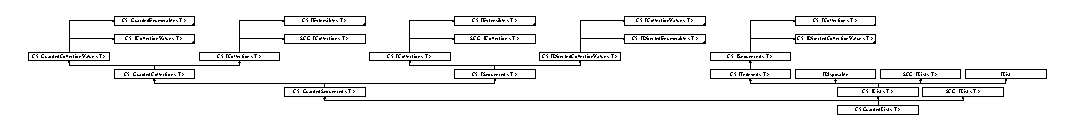
\includegraphics[height=1.314554cm]{class_c5_1_1_guarded_list}
\end{center}
\end{figure}
\subsection*{Public Member Functions}
\begin{DoxyCompactItemize}
\item 
\hyperlink{class_c5_1_1_guarded_list_ae80b0033a55936d85e35dd81c61b9ef8}{Guarded\+List} (\hyperlink{interface_c5_1_1_i_list}{I\+List}$<$ T $>$ list)
\begin{DoxyCompactList}\small\item\em Wrap a list in a read-\/only wrapper. A list gets wrapped as read-\/only, a list view gets wrapped as read-\/only and non-\/slidable. \end{DoxyCompactList}\item 
void \hyperlink{class_c5_1_1_guarded_list_acfdc8f5697d7ad487c9da4c00d15ff4a}{Insert} (int index, T item)
\item 
void \hyperlink{class_c5_1_1_guarded_list_ae15de88d818447d3b25217d1b1298f27}{Insert} (\hyperlink{interface_c5_1_1_i_list}{I\+List}$<$ T $>$ pointer, T item)
\item 
void \hyperlink{class_c5_1_1_guarded_list_a5f5b548fa5704e9a9d83532280a3a0b0}{Insert\+First} (T item)
\item 
void \hyperlink{class_c5_1_1_guarded_list_a0e0d36df19f7bdedf7c9929953381ab5}{Insert\+Last} (T item)
\item 
void \hyperlink{class_c5_1_1_guarded_list_a379efdebd6c5fde83aadf6fd01467a67}{Insert\+Before} (T item, T target)
\item 
void \hyperlink{class_c5_1_1_guarded_list_aeb382caf5b28db625ad150f7ea38511d}{Insert\+After} (T item, T target)
\item 
void \hyperlink{class_c5_1_1_guarded_list_ac87627af2f8b971c1c079e63e64b9953}{Insert\+All} (int i, S\+C\+G.\+I\+Enumerable$<$ T $>$ items)
\item 
\hyperlink{interface_c5_1_1_i_list}{I\+List}$<$ T $>$ \hyperlink{class_c5_1_1_guarded_list_a33bf64be5a6c3affeaba0e652c338811}{Find\+All} (Func$<$ T, bool $>$ filter)
\begin{DoxyCompactList}\small\item\em Perform Find\+All on the wrapped list. The result is {\bfseries not} necessarily read-\/only. \end{DoxyCompactList}\item 
\hyperlink{interface_c5_1_1_i_list}{I\+List}$<$ V $>$ \hyperlink{class_c5_1_1_guarded_list_a383354c45a2b2edd71d58517a1e82920}{Map$<$ V $>$} (Func$<$ T, V $>$ mapper)
\begin{DoxyCompactList}\small\item\em Perform Map on the wrapped list. The result is {\bfseries not} necessarily read-\/only. \end{DoxyCompactList}\item 
\hyperlink{interface_c5_1_1_i_list}{I\+List}$<$ V $>$ \hyperlink{class_c5_1_1_guarded_list_a468610da48a606cd83a609bd116d277c}{Map$<$ V $>$} (Func$<$ T, V $>$ mapper, S\+C\+G.\+I\+Equality\+Comparer$<$ V $>$ itemequality\+Comparer)
\begin{DoxyCompactList}\small\item\em Perform Map on the wrapped list. The result is {\bfseries not} necessarily read-\/only. \end{DoxyCompactList}\item 
T \hyperlink{class_c5_1_1_guarded_list_afdeda008aae91bbbe607012e0e64bac4}{Remove} ()
\item 
T \hyperlink{class_c5_1_1_guarded_list_a5cc22aac9bcdf45c68a285c21e8d1b8d}{Remove\+First} ()
\item 
T \hyperlink{class_c5_1_1_guarded_list_abd9f4b23595221985b5b329b245c0abc}{Remove\+Last} ()
\item 
\hyperlink{interface_c5_1_1_i_list}{I\+List}$<$ T $>$ \hyperlink{class_c5_1_1_guarded_list_affee649b70a9ef563a307f9dbedd04df}{View} (int start, int count)
\begin{DoxyCompactList}\small\item\em Create the indicated view on the wrapped list and wrap it read-\/only. \end{DoxyCompactList}\item 
\hyperlink{interface_c5_1_1_i_list}{I\+List}$<$ T $>$ \hyperlink{class_c5_1_1_guarded_list_a62921460eae17301a85a077aa26e98e3}{View\+Of} (T item)
\begin{DoxyCompactList}\small\item\em Create the indicated view on the wrapped list and wrap it read-\/only. \end{DoxyCompactList}\item 
\hyperlink{interface_c5_1_1_i_list}{I\+List}$<$ T $>$ \hyperlink{class_c5_1_1_guarded_list_a48deee08c78c1e766fb4bbbbf88dc83a}{Last\+View\+Of} (T item)
\begin{DoxyCompactList}\small\item\em Create the indicated view on the wrapped list and wrap it read-\/only. \end{DoxyCompactList}\item 
\hyperlink{interface_c5_1_1_i_list}{I\+List}$<$ T $>$ \hyperlink{class_c5_1_1_guarded_list_a3faccf4fac5e82c8d247b454c3480d81}{Slide} (int offset)
\item 
\hyperlink{interface_c5_1_1_i_list}{I\+List}$<$ T $>$ \hyperlink{class_c5_1_1_guarded_list_a0ce13254cd6bbac5a432abd0ce087871}{Slide} (int offset, int size)
\item 
bool \hyperlink{class_c5_1_1_guarded_list_a6f223ae232ecbcaf3ce345fb86b6e3fd}{Try\+Slide} (int offset)
\item 
bool \hyperlink{class_c5_1_1_guarded_list_aa7279ed330a84a39007653b6cad41b54}{Try\+Slide} (int offset, int size)
\item 
\hyperlink{interface_c5_1_1_i_list}{I\+List}$<$ T $>$ \hyperlink{class_c5_1_1_guarded_list_a4e0d1abd08021423cef51045659bb0c3}{Span} (\hyperlink{interface_c5_1_1_i_list}{I\+List}$<$ T $>$ other\+View)
\item 
void \hyperlink{class_c5_1_1_guarded_list_a22e4adae5aa8ea5588dd9828257e9e65}{Reverse} ()
\begin{DoxyCompactList}\small\item\em 
\begin{DoxyExceptions}{Exceptions}
{\em \hyperlink{class_c5_1_1_read_only_collection_exception}{Read\+Only\+Collection\+Exception}} & since this is a read-\/only wrappper\\
\hline
\end{DoxyExceptions}
\end{DoxyCompactList}\item 
void \hyperlink{class_c5_1_1_guarded_list_aba5504744b39e081df582fe55c958652}{Reverse} (int start, int count)
\item 
bool \hyperlink{class_c5_1_1_guarded_list_a7f201d294ec23f1231ddf27350657537}{Is\+Sorted} ()
\begin{DoxyCompactList}\small\item\em Check if wrapped list is sorted according to the default sorting order for the item type T, as defined by the T\+:\+C5.\+Comparer`1 class \end{DoxyCompactList}\item 
bool \hyperlink{class_c5_1_1_guarded_list_a1a24999c136d34605f5d6b2f004e8610}{Is\+Sorted} (S\+C\+G.\+I\+Comparer$<$ T $>$ c)
\begin{DoxyCompactList}\small\item\em Check if wrapped list is sorted \end{DoxyCompactList}\item 
void \hyperlink{class_c5_1_1_guarded_list_abbc6eedd317b8fb232dd803739867d72}{Sort} ()
\item 
void \hyperlink{class_c5_1_1_guarded_list_a8db443ee1d6d3aec4e55d772c7c14068}{Sort} (S\+C\+G.\+I\+Comparer$<$ T $>$ c)
\item 
void \hyperlink{class_c5_1_1_guarded_list_af01b219433c2383bdaab93e41c9fa589}{Shuffle} ()
\item 
void \hyperlink{class_c5_1_1_guarded_list_a10a56b270623e62b28c1fa848289d6b7}{Shuffle} (Random rnd)
\item 
int \hyperlink{class_c5_1_1_guarded_list_aac2b7de89c7556b8a1c0b49dad25174f}{Index\+Of} (T item)
\begin{DoxyCompactList}\small\item\em Find the (first) index of an item in the wrapped collection \end{DoxyCompactList}\item 
int \hyperlink{class_c5_1_1_guarded_list_a6813134b41bdb0f98b473f02800809c2}{Last\+Index\+Of} (T item)
\begin{DoxyCompactList}\small\item\em Find the last index of an item in the wrapped collection \end{DoxyCompactList}\item 
T \hyperlink{class_c5_1_1_guarded_list_a051deb35bed74f188be08a40c1e79afa}{Remove\+At} (int i)
\item 
void \hyperlink{class_c5_1_1_guarded_list_addc4ab1ca7eb4bf0daebf4453d1397e5}{Remove\+Interval} (int start, int count)
\item 
void \hyperlink{class_c5_1_1_guarded_list_aeb1663686b78f82ab36c5b1dea6812bf}{Push} (T item)
\item 
T \hyperlink{class_c5_1_1_guarded_list_a3876da9aae71b1b0e5deb93c30b26590}{Pop} ()
\item 
void \hyperlink{class_c5_1_1_guarded_list_aac03b7356764f1dd73b8f3bc17007a5e}{Enqueue} (T item)
\item 
T \hyperlink{class_c5_1_1_guarded_list_a5f1cd1c1d41e867c4551ca09ab11e193}{Dequeue} ()
\item 
void \hyperlink{class_c5_1_1_guarded_list_a58d8480779038215c09fcf1b4b80396a}{Dispose} ()
\begin{DoxyCompactList}\small\item\em Ignore\+: this may be called by a foreach or using statement. \end{DoxyCompactList}\end{DoxyCompactItemize}
\subsection*{Properties}
\begin{DoxyCompactItemize}
\item 
T \hyperlink{class_c5_1_1_guarded_list_a3bb363d3e068cef40c9fabfc68bb16c9}{First}\hspace{0.3cm}{\ttfamily  \mbox{[}get\mbox{]}}
\item 
T \hyperlink{class_c5_1_1_guarded_list_a349b68d991e7be0f5c46e9f0d6031fb8}{Last}\hspace{0.3cm}{\ttfamily  \mbox{[}get\mbox{]}}
\item 
bool \hyperlink{class_c5_1_1_guarded_list_a9319f85c3a8830d606126743172d00e6}{F\+I\+F\+O}\hspace{0.3cm}{\ttfamily  \mbox{[}get, set\mbox{]}}
\item 
virtual bool \hyperlink{class_c5_1_1_guarded_list_acbe8502e77878bf3c50eacd4879e5909}{Is\+Fixed\+Size}\hspace{0.3cm}{\ttfamily  \mbox{[}get\mbox{]}}
\item 
T \hyperlink{class_c5_1_1_guarded_list_ad5bc647309e81616d984c7713e4c84ff}{this\mbox{[}int i\mbox{]}}\hspace{0.3cm}{\ttfamily  \mbox{[}get, set\mbox{]}}
\item 
virtual \hyperlink{namespace_c5_a615ba88dcdaa8d5a3c5f833a73d7fad6}{Speed} \hyperlink{class_c5_1_1_guarded_list_a153a69e81c48e5a2905fceb726aebc9e}{Indexing\+Speed}\hspace{0.3cm}{\ttfamily  \mbox{[}get\mbox{]}}
\item 
\hyperlink{interface_c5_1_1_i_list}{I\+List}$<$ T $>$ \hyperlink{class_c5_1_1_guarded_list_af6565bed0e461d28b7f125481d22cc5f}{Underlying}\hspace{0.3cm}{\ttfamily  \mbox{[}get\mbox{]}}
\item 
int \hyperlink{class_c5_1_1_guarded_list_afcec36d0e79fd5634866b62065f51d49}{Offset}\hspace{0.3cm}{\ttfamily  \mbox{[}get\mbox{]}}
\item 
virtual bool \hyperlink{class_c5_1_1_guarded_list_a9f6857e8494abd309c9b4f4f92e5ab09}{Is\+Valid}\hspace{0.3cm}{\ttfamily  \mbox{[}get\mbox{]}}
\item 
\hyperlink{interface_c5_1_1_i_directed_collection_value}{I\+Directed\+Collection\+Value}$<$ T $>$ \hyperlink{class_c5_1_1_guarded_list_a3aa22d62b09f2a0180cc5c1342eb4ce4}{this\mbox{[}int start, int end\mbox{]}}\hspace{0.3cm}{\ttfamily  \mbox{[}get\mbox{]}}
\end{DoxyCompactItemize}
\subsection*{Additional Inherited Members}


\subsection{Detailed Description}
A read-\/only wrapper for a generic list collection {\itshape Suitable as a wrapper for \hyperlink{class_c5_1_1_linked_list}{Linked\+List}, \hyperlink{class_c5_1_1_hashed_linked_list}{Hashed\+Linked\+List}, \hyperlink{class_c5_1_1_array_list}{Array\+List} and Hashed\+Array. T\+:\+C5.\+Linked\+List`1, T\+:\+C5.\+Hashed\+Linked\+List`1, T\+:\+C5.\+Array\+List`1 or T\+:\+C5.\+Hashed\+Array`1. } 



\subsection{Constructor \& Destructor Documentation}
\hypertarget{class_c5_1_1_guarded_list_ae80b0033a55936d85e35dd81c61b9ef8}{}\index{C5\+::\+Guarded\+List@{C5\+::\+Guarded\+List}!Guarded\+List@{Guarded\+List}}
\index{Guarded\+List@{Guarded\+List}!C5\+::\+Guarded\+List@{C5\+::\+Guarded\+List}}
\subsubsection[{Guarded\+List(\+I\+List$<$ T $>$ list)}]{\setlength{\rightskip}{0pt plus 5cm}{\bf C5.\+Guarded\+List}$<$ T $>$.{\bf Guarded\+List} (
\begin{DoxyParamCaption}
\item[{{\bf I\+List}$<$ T $>$}]{list}
\end{DoxyParamCaption}
)}\label{class_c5_1_1_guarded_list_ae80b0033a55936d85e35dd81c61b9ef8}


Wrap a list in a read-\/only wrapper. A list gets wrapped as read-\/only, a list view gets wrapped as read-\/only and non-\/slidable. 


\begin{DoxyParams}{Parameters}
{\em list} & The list\\
\hline
\end{DoxyParams}


\subsection{Member Function Documentation}
\hypertarget{class_c5_1_1_guarded_list_a5f1cd1c1d41e867c4551ca09ab11e193}{}\index{C5\+::\+Guarded\+List@{C5\+::\+Guarded\+List}!Dequeue@{Dequeue}}
\index{Dequeue@{Dequeue}!C5\+::\+Guarded\+List@{C5\+::\+Guarded\+List}}
\subsubsection[{Dequeue()}]{\setlength{\rightskip}{0pt plus 5cm}T {\bf C5.\+Guarded\+List}$<$ T $>$.Dequeue (
\begin{DoxyParamCaption}
{}
\end{DoxyParamCaption}
)}\label{class_c5_1_1_guarded_list_a5f1cd1c1d41e867c4551ca09ab11e193}





\begin{DoxyExceptions}{Exceptions}
{\em \hyperlink{class_c5_1_1_read_only_collection_exception}{Read\+Only\+Collection\+Exception}} & since this is a read-\/only wrappper\\
\hline
\end{DoxyExceptions}
\begin{DoxyReturn}{Returns}
-\/
\end{DoxyReturn}
\hypertarget{class_c5_1_1_guarded_list_a58d8480779038215c09fcf1b4b80396a}{}\index{C5\+::\+Guarded\+List@{C5\+::\+Guarded\+List}!Dispose@{Dispose}}
\index{Dispose@{Dispose}!C5\+::\+Guarded\+List@{C5\+::\+Guarded\+List}}
\subsubsection[{Dispose()}]{\setlength{\rightskip}{0pt plus 5cm}void {\bf C5.\+Guarded\+List}$<$ T $>$.Dispose (
\begin{DoxyParamCaption}
{}
\end{DoxyParamCaption}
)}\label{class_c5_1_1_guarded_list_a58d8480779038215c09fcf1b4b80396a}


Ignore\+: this may be called by a foreach or using statement. 

\hypertarget{class_c5_1_1_guarded_list_aac03b7356764f1dd73b8f3bc17007a5e}{}\index{C5\+::\+Guarded\+List@{C5\+::\+Guarded\+List}!Enqueue@{Enqueue}}
\index{Enqueue@{Enqueue}!C5\+::\+Guarded\+List@{C5\+::\+Guarded\+List}}
\subsubsection[{Enqueue(\+T item)}]{\setlength{\rightskip}{0pt plus 5cm}void {\bf C5.\+Guarded\+List}$<$ T $>$.Enqueue (
\begin{DoxyParamCaption}
\item[{T}]{item}
\end{DoxyParamCaption}
)}\label{class_c5_1_1_guarded_list_aac03b7356764f1dd73b8f3bc17007a5e}





\begin{DoxyExceptions}{Exceptions}
{\em \hyperlink{class_c5_1_1_read_only_collection_exception}{Read\+Only\+Collection\+Exception}} & since this is a read-\/only wrappper\\
\hline
\end{DoxyExceptions}
\begin{DoxyReturn}{Returns}
-\/
\end{DoxyReturn}
\hypertarget{class_c5_1_1_guarded_list_a33bf64be5a6c3affeaba0e652c338811}{}\index{C5\+::\+Guarded\+List@{C5\+::\+Guarded\+List}!Find\+All@{Find\+All}}
\index{Find\+All@{Find\+All}!C5\+::\+Guarded\+List@{C5\+::\+Guarded\+List}}
\subsubsection[{Find\+All(\+Func$<$ T, bool $>$ filter)}]{\setlength{\rightskip}{0pt plus 5cm}{\bf I\+List}$<$T$>$ {\bf C5.\+Guarded\+List}$<$ T $>$.Find\+All (
\begin{DoxyParamCaption}
\item[{Func$<$ T, bool $>$}]{filter}
\end{DoxyParamCaption}
)}\label{class_c5_1_1_guarded_list_a33bf64be5a6c3affeaba0e652c338811}


Perform Find\+All on the wrapped list. The result is {\bfseries not} necessarily read-\/only. 


\begin{DoxyParams}{Parameters}
{\em filter} & The filter to use\\
\hline
\end{DoxyParams}
\begin{DoxyReturn}{Returns}

\end{DoxyReturn}


Implements \hyperlink{interface_c5_1_1_i_list_a8bd6c307e2b3e5cbd50e92dde854a1d0}{C5.\+I\+List$<$ T $>$}.

\hypertarget{class_c5_1_1_guarded_list_aac2b7de89c7556b8a1c0b49dad25174f}{}\index{C5\+::\+Guarded\+List@{C5\+::\+Guarded\+List}!Index\+Of@{Index\+Of}}
\index{Index\+Of@{Index\+Of}!C5\+::\+Guarded\+List@{C5\+::\+Guarded\+List}}
\subsubsection[{Index\+Of(\+T item)}]{\setlength{\rightskip}{0pt plus 5cm}int {\bf C5.\+Guarded\+List}$<$ T $>$.Index\+Of (
\begin{DoxyParamCaption}
\item[{T}]{item}
\end{DoxyParamCaption}
)}\label{class_c5_1_1_guarded_list_aac2b7de89c7556b8a1c0b49dad25174f}


Find the (first) index of an item in the wrapped collection 


\begin{DoxyParams}{Parameters}
{\em item} & \\
\hline
\end{DoxyParams}
\begin{DoxyReturn}{Returns}

\end{DoxyReturn}


Implements \hyperlink{interface_c5_1_1_i_list_a52658ee618f1557622d766d7a348910a}{C5.\+I\+List$<$ T $>$}.

\hypertarget{class_c5_1_1_guarded_list_acfdc8f5697d7ad487c9da4c00d15ff4a}{}\index{C5\+::\+Guarded\+List@{C5\+::\+Guarded\+List}!Insert@{Insert}}
\index{Insert@{Insert}!C5\+::\+Guarded\+List@{C5\+::\+Guarded\+List}}
\subsubsection[{Insert(int index, T item)}]{\setlength{\rightskip}{0pt plus 5cm}void {\bf C5.\+Guarded\+List}$<$ T $>$.Insert (
\begin{DoxyParamCaption}
\item[{int}]{index, }
\item[{T}]{item}
\end{DoxyParamCaption}
)}\label{class_c5_1_1_guarded_list_acfdc8f5697d7ad487c9da4c00d15ff4a}





\begin{DoxyExceptions}{Exceptions}
{\em \hyperlink{class_c5_1_1_read_only_collection_exception}{Read\+Only\+Collection\+Exception}} & since this is a read-\/only wrappper\\
\hline
\end{DoxyExceptions}

\begin{DoxyParams}{Parameters}
{\em index} & \\
\hline
{\em item} & \\
\hline
\end{DoxyParams}
\hypertarget{class_c5_1_1_guarded_list_ae15de88d818447d3b25217d1b1298f27}{}\index{C5\+::\+Guarded\+List@{C5\+::\+Guarded\+List}!Insert@{Insert}}
\index{Insert@{Insert}!C5\+::\+Guarded\+List@{C5\+::\+Guarded\+List}}
\subsubsection[{Insert(\+I\+List$<$ T $>$ pointer, T item)}]{\setlength{\rightskip}{0pt plus 5cm}void {\bf C5.\+Guarded\+List}$<$ T $>$.Insert (
\begin{DoxyParamCaption}
\item[{{\bf I\+List}$<$ T $>$}]{pointer, }
\item[{T}]{item}
\end{DoxyParamCaption}
)}\label{class_c5_1_1_guarded_list_ae15de88d818447d3b25217d1b1298f27}





\begin{DoxyExceptions}{Exceptions}
{\em \hyperlink{class_c5_1_1_read_only_collection_exception}{Read\+Only\+Collection\+Exception}} & since this is a read-\/only wrappper\\
\hline
\end{DoxyExceptions}

\begin{DoxyParams}{Parameters}
{\em pointer} & \\
\hline
{\em item} & \\
\hline
\end{DoxyParams}


Implements \hyperlink{interface_c5_1_1_i_list_a80df9055583216f4498d3711c9658d1f}{C5.\+I\+List$<$ T $>$}.

\hypertarget{class_c5_1_1_guarded_list_aeb382caf5b28db625ad150f7ea38511d}{}\index{C5\+::\+Guarded\+List@{C5\+::\+Guarded\+List}!Insert\+After@{Insert\+After}}
\index{Insert\+After@{Insert\+After}!C5\+::\+Guarded\+List@{C5\+::\+Guarded\+List}}
\subsubsection[{Insert\+After(\+T item, T target)}]{\setlength{\rightskip}{0pt plus 5cm}void {\bf C5.\+Guarded\+List}$<$ T $>$.Insert\+After (
\begin{DoxyParamCaption}
\item[{T}]{item, }
\item[{T}]{target}
\end{DoxyParamCaption}
)}\label{class_c5_1_1_guarded_list_aeb382caf5b28db625ad150f7ea38511d}





\begin{DoxyExceptions}{Exceptions}
{\em \hyperlink{class_c5_1_1_read_only_collection_exception}{Read\+Only\+Collection\+Exception}} & since this is a read-\/only wrappper\\
\hline
\end{DoxyExceptions}

\begin{DoxyParams}{Parameters}
{\em item} & \\
\hline
{\em target} & \\
\hline
\end{DoxyParams}
\hypertarget{class_c5_1_1_guarded_list_ac87627af2f8b971c1c079e63e64b9953}{}\index{C5\+::\+Guarded\+List@{C5\+::\+Guarded\+List}!Insert\+All@{Insert\+All}}
\index{Insert\+All@{Insert\+All}!C5\+::\+Guarded\+List@{C5\+::\+Guarded\+List}}
\subsubsection[{Insert\+All(int i, S\+C\+G.\+I\+Enumerable$<$ T $>$ items)}]{\setlength{\rightskip}{0pt plus 5cm}void {\bf C5.\+Guarded\+List}$<$ T $>$.Insert\+All (
\begin{DoxyParamCaption}
\item[{int}]{i, }
\item[{S\+C\+G.\+I\+Enumerable$<$ T $>$}]{items}
\end{DoxyParamCaption}
)}\label{class_c5_1_1_guarded_list_ac87627af2f8b971c1c079e63e64b9953}





\begin{DoxyExceptions}{Exceptions}
{\em \hyperlink{class_c5_1_1_read_only_collection_exception}{Read\+Only\+Collection\+Exception}} & since this is a read-\/only wrappper\\
\hline
\end{DoxyExceptions}

\begin{DoxyParams}{Parameters}
{\em i} & \\
\hline
{\em items} & \\
\hline
\end{DoxyParams}


Implements \hyperlink{interface_c5_1_1_i_list_a551f34466ccd64b90929d8a92b984dc5}{C5.\+I\+List$<$ T $>$}.

\hypertarget{class_c5_1_1_guarded_list_a379efdebd6c5fde83aadf6fd01467a67}{}\index{C5\+::\+Guarded\+List@{C5\+::\+Guarded\+List}!Insert\+Before@{Insert\+Before}}
\index{Insert\+Before@{Insert\+Before}!C5\+::\+Guarded\+List@{C5\+::\+Guarded\+List}}
\subsubsection[{Insert\+Before(\+T item, T target)}]{\setlength{\rightskip}{0pt plus 5cm}void {\bf C5.\+Guarded\+List}$<$ T $>$.Insert\+Before (
\begin{DoxyParamCaption}
\item[{T}]{item, }
\item[{T}]{target}
\end{DoxyParamCaption}
)}\label{class_c5_1_1_guarded_list_a379efdebd6c5fde83aadf6fd01467a67}





\begin{DoxyExceptions}{Exceptions}
{\em \hyperlink{class_c5_1_1_read_only_collection_exception}{Read\+Only\+Collection\+Exception}} & since this is a read-\/only wrappper\\
\hline
\end{DoxyExceptions}

\begin{DoxyParams}{Parameters}
{\em item} & \\
\hline
{\em target} & \\
\hline
\end{DoxyParams}
\hypertarget{class_c5_1_1_guarded_list_a5f5b548fa5704e9a9d83532280a3a0b0}{}\index{C5\+::\+Guarded\+List@{C5\+::\+Guarded\+List}!Insert\+First@{Insert\+First}}
\index{Insert\+First@{Insert\+First}!C5\+::\+Guarded\+List@{C5\+::\+Guarded\+List}}
\subsubsection[{Insert\+First(\+T item)}]{\setlength{\rightskip}{0pt plus 5cm}void {\bf C5.\+Guarded\+List}$<$ T $>$.Insert\+First (
\begin{DoxyParamCaption}
\item[{T}]{item}
\end{DoxyParamCaption}
)}\label{class_c5_1_1_guarded_list_a5f5b548fa5704e9a9d83532280a3a0b0}





\begin{DoxyExceptions}{Exceptions}
{\em \hyperlink{class_c5_1_1_read_only_collection_exception}{Read\+Only\+Collection\+Exception}} & since this is a read-\/only wrappper\\
\hline
\end{DoxyExceptions}

\begin{DoxyParams}{Parameters}
{\em item} & \\
\hline
\end{DoxyParams}


Implements \hyperlink{interface_c5_1_1_i_list_a2dd0bf119dee26610ce56283da7d7d11}{C5.\+I\+List$<$ T $>$}.

\hypertarget{class_c5_1_1_guarded_list_a0e0d36df19f7bdedf7c9929953381ab5}{}\index{C5\+::\+Guarded\+List@{C5\+::\+Guarded\+List}!Insert\+Last@{Insert\+Last}}
\index{Insert\+Last@{Insert\+Last}!C5\+::\+Guarded\+List@{C5\+::\+Guarded\+List}}
\subsubsection[{Insert\+Last(\+T item)}]{\setlength{\rightskip}{0pt plus 5cm}void {\bf C5.\+Guarded\+List}$<$ T $>$.Insert\+Last (
\begin{DoxyParamCaption}
\item[{T}]{item}
\end{DoxyParamCaption}
)}\label{class_c5_1_1_guarded_list_a0e0d36df19f7bdedf7c9929953381ab5}





\begin{DoxyExceptions}{Exceptions}
{\em \hyperlink{class_c5_1_1_read_only_collection_exception}{Read\+Only\+Collection\+Exception}} & since this is a read-\/only wrappper\\
\hline
\end{DoxyExceptions}

\begin{DoxyParams}{Parameters}
{\em item} & \\
\hline
\end{DoxyParams}


Implements \hyperlink{interface_c5_1_1_i_list_adbb76aa84c81cf3d93130ed3d3abd967}{C5.\+I\+List$<$ T $>$}.

\hypertarget{class_c5_1_1_guarded_list_a7f201d294ec23f1231ddf27350657537}{}\index{C5\+::\+Guarded\+List@{C5\+::\+Guarded\+List}!Is\+Sorted@{Is\+Sorted}}
\index{Is\+Sorted@{Is\+Sorted}!C5\+::\+Guarded\+List@{C5\+::\+Guarded\+List}}
\subsubsection[{Is\+Sorted()}]{\setlength{\rightskip}{0pt plus 5cm}bool {\bf C5.\+Guarded\+List}$<$ T $>$.Is\+Sorted (
\begin{DoxyParamCaption}
{}
\end{DoxyParamCaption}
)}\label{class_c5_1_1_guarded_list_a7f201d294ec23f1231ddf27350657537}


Check if wrapped list is sorted according to the default sorting order for the item type T, as defined by the T\+:\+C5.\+Comparer`1 class 


\begin{DoxyExceptions}{Exceptions}
{\em \hyperlink{class_c5_1_1_not_comparable_exception}{Not\+Comparable\+Exception}} & if T is not comparable\\
\hline
\end{DoxyExceptions}
\begin{DoxyReturn}{Returns}
True if the list is sorted, else false.
\end{DoxyReturn}


Implements \hyperlink{interface_c5_1_1_i_list_aadf94b51e2c383ebda5a9f48820ef9bb}{C5.\+I\+List$<$ T $>$}.

\hypertarget{class_c5_1_1_guarded_list_a1a24999c136d34605f5d6b2f004e8610}{}\index{C5\+::\+Guarded\+List@{C5\+::\+Guarded\+List}!Is\+Sorted@{Is\+Sorted}}
\index{Is\+Sorted@{Is\+Sorted}!C5\+::\+Guarded\+List@{C5\+::\+Guarded\+List}}
\subsubsection[{Is\+Sorted(\+S\+C\+G.\+I\+Comparer$<$ T $>$ c)}]{\setlength{\rightskip}{0pt plus 5cm}bool {\bf C5.\+Guarded\+List}$<$ T $>$.Is\+Sorted (
\begin{DoxyParamCaption}
\item[{S\+C\+G.\+I\+Comparer$<$ T $>$}]{c}
\end{DoxyParamCaption}
)}\label{class_c5_1_1_guarded_list_a1a24999c136d34605f5d6b2f004e8610}


Check if wrapped list is sorted 


\begin{DoxyParams}{Parameters}
{\em c} & The sorting order to use\\
\hline
\end{DoxyParams}
\begin{DoxyReturn}{Returns}
True if sorted
\end{DoxyReturn}


Implements \hyperlink{interface_c5_1_1_i_list_ad7a87f535eab2f950eb4ad3311f3385f}{C5.\+I\+List$<$ T $>$}.

\hypertarget{class_c5_1_1_guarded_list_a6813134b41bdb0f98b473f02800809c2}{}\index{C5\+::\+Guarded\+List@{C5\+::\+Guarded\+List}!Last\+Index\+Of@{Last\+Index\+Of}}
\index{Last\+Index\+Of@{Last\+Index\+Of}!C5\+::\+Guarded\+List@{C5\+::\+Guarded\+List}}
\subsubsection[{Last\+Index\+Of(\+T item)}]{\setlength{\rightskip}{0pt plus 5cm}int {\bf C5.\+Guarded\+List}$<$ T $>$.Last\+Index\+Of (
\begin{DoxyParamCaption}
\item[{T}]{item}
\end{DoxyParamCaption}
)}\label{class_c5_1_1_guarded_list_a6813134b41bdb0f98b473f02800809c2}


Find the last index of an item in the wrapped collection 


\begin{DoxyParams}{Parameters}
{\em item} & \\
\hline
\end{DoxyParams}
\begin{DoxyReturn}{Returns}

\end{DoxyReturn}


Implements \hyperlink{interface_c5_1_1_i_indexed_a50f274e0f7b4cd2e54db4cb61a003b95}{C5.\+I\+Indexed$<$ T $>$}.

\hypertarget{class_c5_1_1_guarded_list_a48deee08c78c1e766fb4bbbbf88dc83a}{}\index{C5\+::\+Guarded\+List@{C5\+::\+Guarded\+List}!Last\+View\+Of@{Last\+View\+Of}}
\index{Last\+View\+Of@{Last\+View\+Of}!C5\+::\+Guarded\+List@{C5\+::\+Guarded\+List}}
\subsubsection[{Last\+View\+Of(\+T item)}]{\setlength{\rightskip}{0pt plus 5cm}{\bf I\+List}$<$T$>$ {\bf C5.\+Guarded\+List}$<$ T $>$.Last\+View\+Of (
\begin{DoxyParamCaption}
\item[{T}]{item}
\end{DoxyParamCaption}
)}\label{class_c5_1_1_guarded_list_a48deee08c78c1e766fb4bbbbf88dc83a}


Create the indicated view on the wrapped list and wrap it read-\/only. 


\begin{DoxyParams}{Parameters}
{\em item} & \\
\hline
\end{DoxyParams}
\begin{DoxyReturn}{Returns}

\end{DoxyReturn}


Implements \hyperlink{interface_c5_1_1_i_list_a251c36fe72c9bc661d449bfd0ea90528}{C5.\+I\+List$<$ T $>$}.

\hypertarget{class_c5_1_1_guarded_list_a383354c45a2b2edd71d58517a1e82920}{}\index{C5\+::\+Guarded\+List@{C5\+::\+Guarded\+List}!Map$<$ V $>$@{Map$<$ V $>$}}
\index{Map$<$ V $>$@{Map$<$ V $>$}!C5\+::\+Guarded\+List@{C5\+::\+Guarded\+List}}
\subsubsection[{Map$<$ V $>$(\+Func$<$ T, V $>$ mapper)}]{\setlength{\rightskip}{0pt plus 5cm}{\bf I\+List}$<$V$>$ {\bf C5.\+Guarded\+List}$<$ T $>$.Map$<$ V $>$ (
\begin{DoxyParamCaption}
\item[{Func$<$ T, V $>$}]{mapper}
\end{DoxyParamCaption}
)}\label{class_c5_1_1_guarded_list_a383354c45a2b2edd71d58517a1e82920}


Perform Map on the wrapped list. The result is {\bfseries not} necessarily read-\/only. 


\begin{DoxyTemplParams}{Template Parameters}
{\em V} & The type of items of the new list\\
\hline
\end{DoxyTemplParams}

\begin{DoxyParams}{Parameters}
{\em mapper} & The mapper to use.\\
\hline
\end{DoxyParams}
\begin{DoxyReturn}{Returns}
The mapped list
\end{DoxyReturn}


Implements \hyperlink{interface_c5_1_1_i_list_a8cf8a4682fe990ce32d7cf4a2bec84b6}{C5.\+I\+List$<$ T $>$}.

\hypertarget{class_c5_1_1_guarded_list_a468610da48a606cd83a609bd116d277c}{}\index{C5\+::\+Guarded\+List@{C5\+::\+Guarded\+List}!Map$<$ V $>$@{Map$<$ V $>$}}
\index{Map$<$ V $>$@{Map$<$ V $>$}!C5\+::\+Guarded\+List@{C5\+::\+Guarded\+List}}
\subsubsection[{Map$<$ V $>$(\+Func$<$ T, V $>$ mapper, S\+C\+G.\+I\+Equality\+Comparer$<$ V $>$ itemequality\+Comparer)}]{\setlength{\rightskip}{0pt plus 5cm}{\bf I\+List}$<$V$>$ {\bf C5.\+Guarded\+List}$<$ T $>$.Map$<$ V $>$ (
\begin{DoxyParamCaption}
\item[{Func$<$ T, V $>$}]{mapper, }
\item[{S\+C\+G.\+I\+Equality\+Comparer$<$ V $>$}]{itemequality\+Comparer}
\end{DoxyParamCaption}
)}\label{class_c5_1_1_guarded_list_a468610da48a606cd83a609bd116d277c}


Perform Map on the wrapped list. The result is {\bfseries not} necessarily read-\/only. 


\begin{DoxyTemplParams}{Template Parameters}
{\em V} & The type of items of the new list\\
\hline
\end{DoxyTemplParams}

\begin{DoxyParams}{Parameters}
{\em mapper} & The delegate defining the map.\\
\hline
{\em itemequality\+Comparer} & The itemequality\+Comparer to use for the new list\\
\hline
\end{DoxyParams}
\begin{DoxyReturn}{Returns}
The new list.
\end{DoxyReturn}


Implements \hyperlink{interface_c5_1_1_i_list_ad84aa90d1111a8cb7ea1226d8cfadab9}{C5.\+I\+List$<$ T $>$}.

\hypertarget{class_c5_1_1_guarded_list_a3876da9aae71b1b0e5deb93c30b26590}{}\index{C5\+::\+Guarded\+List@{C5\+::\+Guarded\+List}!Pop@{Pop}}
\index{Pop@{Pop}!C5\+::\+Guarded\+List@{C5\+::\+Guarded\+List}}
\subsubsection[{Pop()}]{\setlength{\rightskip}{0pt plus 5cm}T {\bf C5.\+Guarded\+List}$<$ T $>$.Pop (
\begin{DoxyParamCaption}
{}
\end{DoxyParamCaption}
)}\label{class_c5_1_1_guarded_list_a3876da9aae71b1b0e5deb93c30b26590}





\begin{DoxyExceptions}{Exceptions}
{\em \hyperlink{class_c5_1_1_read_only_collection_exception}{Read\+Only\+Collection\+Exception}} & since this is a read-\/only wrappper\\
\hline
\end{DoxyExceptions}
\begin{DoxyReturn}{Returns}
-\/
\end{DoxyReturn}
\hypertarget{class_c5_1_1_guarded_list_aeb1663686b78f82ab36c5b1dea6812bf}{}\index{C5\+::\+Guarded\+List@{C5\+::\+Guarded\+List}!Push@{Push}}
\index{Push@{Push}!C5\+::\+Guarded\+List@{C5\+::\+Guarded\+List}}
\subsubsection[{Push(\+T item)}]{\setlength{\rightskip}{0pt plus 5cm}void {\bf C5.\+Guarded\+List}$<$ T $>$.Push (
\begin{DoxyParamCaption}
\item[{T}]{item}
\end{DoxyParamCaption}
)}\label{class_c5_1_1_guarded_list_aeb1663686b78f82ab36c5b1dea6812bf}





\begin{DoxyExceptions}{Exceptions}
{\em \hyperlink{class_c5_1_1_read_only_collection_exception}{Read\+Only\+Collection\+Exception}} & since this is a read-\/only wrappper\\
\hline
\end{DoxyExceptions}
\begin{DoxyReturn}{Returns}
-\/
\end{DoxyReturn}
\hypertarget{class_c5_1_1_guarded_list_afdeda008aae91bbbe607012e0e64bac4}{}\index{C5\+::\+Guarded\+List@{C5\+::\+Guarded\+List}!Remove@{Remove}}
\index{Remove@{Remove}!C5\+::\+Guarded\+List@{C5\+::\+Guarded\+List}}
\subsubsection[{Remove()}]{\setlength{\rightskip}{0pt plus 5cm}T {\bf C5.\+Guarded\+List}$<$ T $>$.Remove (
\begin{DoxyParamCaption}
{}
\end{DoxyParamCaption}
)}\label{class_c5_1_1_guarded_list_afdeda008aae91bbbe607012e0e64bac4}





\begin{DoxyExceptions}{Exceptions}
{\em \hyperlink{class_c5_1_1_read_only_collection_exception}{Read\+Only\+Collection\+Exception}} & since this is a read-\/only wrappper\\
\hline
\end{DoxyExceptions}
\begin{DoxyReturn}{Returns}

\end{DoxyReturn}


Implements \hyperlink{interface_c5_1_1_i_list_ae0d9be125f478fed048c4c08159ae399}{C5.\+I\+List$<$ T $>$}.

\hypertarget{class_c5_1_1_guarded_list_a051deb35bed74f188be08a40c1e79afa}{}\index{C5\+::\+Guarded\+List@{C5\+::\+Guarded\+List}!Remove\+At@{Remove\+At}}
\index{Remove\+At@{Remove\+At}!C5\+::\+Guarded\+List@{C5\+::\+Guarded\+List}}
\subsubsection[{Remove\+At(int i)}]{\setlength{\rightskip}{0pt plus 5cm}T {\bf C5.\+Guarded\+List}$<$ T $>$.Remove\+At (
\begin{DoxyParamCaption}
\item[{int}]{i}
\end{DoxyParamCaption}
)}\label{class_c5_1_1_guarded_list_a051deb35bed74f188be08a40c1e79afa}





\begin{DoxyExceptions}{Exceptions}
{\em \hyperlink{class_c5_1_1_read_only_collection_exception}{Read\+Only\+Collection\+Exception}} & since this is a read-\/only wrappper\\
\hline
\end{DoxyExceptions}

\begin{DoxyParams}{Parameters}
{\em i} & \\
\hline
\end{DoxyParams}
\begin{DoxyReturn}{Returns}

\end{DoxyReturn}


Implements \hyperlink{interface_c5_1_1_i_list_a9fbcd9c55aae61134321939d0b104cc0}{C5.\+I\+List$<$ T $>$}.

\hypertarget{class_c5_1_1_guarded_list_a5cc22aac9bcdf45c68a285c21e8d1b8d}{}\index{C5\+::\+Guarded\+List@{C5\+::\+Guarded\+List}!Remove\+First@{Remove\+First}}
\index{Remove\+First@{Remove\+First}!C5\+::\+Guarded\+List@{C5\+::\+Guarded\+List}}
\subsubsection[{Remove\+First()}]{\setlength{\rightskip}{0pt plus 5cm}T {\bf C5.\+Guarded\+List}$<$ T $>$.Remove\+First (
\begin{DoxyParamCaption}
{}
\end{DoxyParamCaption}
)}\label{class_c5_1_1_guarded_list_a5cc22aac9bcdf45c68a285c21e8d1b8d}





\begin{DoxyExceptions}{Exceptions}
{\em \hyperlink{class_c5_1_1_read_only_collection_exception}{Read\+Only\+Collection\+Exception}} & since this is a read-\/only wrappper\\
\hline
\end{DoxyExceptions}
\begin{DoxyReturn}{Returns}

\end{DoxyReturn}


Implements \hyperlink{interface_c5_1_1_i_list_a6f5c3f67673d43604aa28a7d2b6508ff}{C5.\+I\+List$<$ T $>$}.

\hypertarget{class_c5_1_1_guarded_list_addc4ab1ca7eb4bf0daebf4453d1397e5}{}\index{C5\+::\+Guarded\+List@{C5\+::\+Guarded\+List}!Remove\+Interval@{Remove\+Interval}}
\index{Remove\+Interval@{Remove\+Interval}!C5\+::\+Guarded\+List@{C5\+::\+Guarded\+List}}
\subsubsection[{Remove\+Interval(int start, int count)}]{\setlength{\rightskip}{0pt plus 5cm}void {\bf C5.\+Guarded\+List}$<$ T $>$.Remove\+Interval (
\begin{DoxyParamCaption}
\item[{int}]{start, }
\item[{int}]{count}
\end{DoxyParamCaption}
)}\label{class_c5_1_1_guarded_list_addc4ab1ca7eb4bf0daebf4453d1397e5}





\begin{DoxyExceptions}{Exceptions}
{\em \hyperlink{class_c5_1_1_read_only_collection_exception}{Read\+Only\+Collection\+Exception}} & since this is a read-\/only wrappper\\
\hline
\end{DoxyExceptions}

\begin{DoxyParams}{Parameters}
{\em start} & \\
\hline
{\em count} & \\
\hline
\end{DoxyParams}


Implements \hyperlink{interface_c5_1_1_i_indexed_aa9d2a1706ba0361079d31c02bad3e810}{C5.\+I\+Indexed$<$ T $>$}.

\hypertarget{class_c5_1_1_guarded_list_abd9f4b23595221985b5b329b245c0abc}{}\index{C5\+::\+Guarded\+List@{C5\+::\+Guarded\+List}!Remove\+Last@{Remove\+Last}}
\index{Remove\+Last@{Remove\+Last}!C5\+::\+Guarded\+List@{C5\+::\+Guarded\+List}}
\subsubsection[{Remove\+Last()}]{\setlength{\rightskip}{0pt plus 5cm}T {\bf C5.\+Guarded\+List}$<$ T $>$.Remove\+Last (
\begin{DoxyParamCaption}
{}
\end{DoxyParamCaption}
)}\label{class_c5_1_1_guarded_list_abd9f4b23595221985b5b329b245c0abc}





\begin{DoxyExceptions}{Exceptions}
{\em \hyperlink{class_c5_1_1_read_only_collection_exception}{Read\+Only\+Collection\+Exception}} & since this is a read-\/only wrappper\\
\hline
\end{DoxyExceptions}
\begin{DoxyReturn}{Returns}

\end{DoxyReturn}


Implements \hyperlink{interface_c5_1_1_i_list_adfbae9e7ea5cb9ff3e0fd45f1201334a}{C5.\+I\+List$<$ T $>$}.

\hypertarget{class_c5_1_1_guarded_list_a22e4adae5aa8ea5588dd9828257e9e65}{}\index{C5\+::\+Guarded\+List@{C5\+::\+Guarded\+List}!Reverse@{Reverse}}
\index{Reverse@{Reverse}!C5\+::\+Guarded\+List@{C5\+::\+Guarded\+List}}
\subsubsection[{Reverse()}]{\setlength{\rightskip}{0pt plus 5cm}void {\bf C5.\+Guarded\+List}$<$ T $>$.Reverse (
\begin{DoxyParamCaption}
{}
\end{DoxyParamCaption}
)}\label{class_c5_1_1_guarded_list_a22e4adae5aa8ea5588dd9828257e9e65}



\begin{DoxyExceptions}{Exceptions}
{\em \hyperlink{class_c5_1_1_read_only_collection_exception}{Read\+Only\+Collection\+Exception}} & since this is a read-\/only wrappper\\
\hline
\end{DoxyExceptions}




Implements \hyperlink{interface_c5_1_1_i_list_aea3fef718431d1ab504e15457e7fda1c}{C5.\+I\+List$<$ T $>$}.

\hypertarget{class_c5_1_1_guarded_list_aba5504744b39e081df582fe55c958652}{}\index{C5\+::\+Guarded\+List@{C5\+::\+Guarded\+List}!Reverse@{Reverse}}
\index{Reverse@{Reverse}!C5\+::\+Guarded\+List@{C5\+::\+Guarded\+List}}
\subsubsection[{Reverse(int start, int count)}]{\setlength{\rightskip}{0pt plus 5cm}void {\bf C5.\+Guarded\+List}$<$ T $>$.Reverse (
\begin{DoxyParamCaption}
\item[{int}]{start, }
\item[{int}]{count}
\end{DoxyParamCaption}
)}\label{class_c5_1_1_guarded_list_aba5504744b39e081df582fe55c958652}





\begin{DoxyExceptions}{Exceptions}
{\em \hyperlink{class_c5_1_1_read_only_collection_exception}{Read\+Only\+Collection\+Exception}} & since this is a read-\/only wrappper\\
\hline
\end{DoxyExceptions}

\begin{DoxyParams}{Parameters}
{\em start} & \\
\hline
{\em count} & \\
\hline
\end{DoxyParams}
\hypertarget{class_c5_1_1_guarded_list_af01b219433c2383bdaab93e41c9fa589}{}\index{C5\+::\+Guarded\+List@{C5\+::\+Guarded\+List}!Shuffle@{Shuffle}}
\index{Shuffle@{Shuffle}!C5\+::\+Guarded\+List@{C5\+::\+Guarded\+List}}
\subsubsection[{Shuffle()}]{\setlength{\rightskip}{0pt plus 5cm}void {\bf C5.\+Guarded\+List}$<$ T $>$.Shuffle (
\begin{DoxyParamCaption}
{}
\end{DoxyParamCaption}
)}\label{class_c5_1_1_guarded_list_af01b219433c2383bdaab93e41c9fa589}





\begin{DoxyExceptions}{Exceptions}
{\em \hyperlink{class_c5_1_1_read_only_collection_exception}{Read\+Only\+Collection\+Exception}} & since this is a read-\/only wrappper\\
\hline
\end{DoxyExceptions}


Implements \hyperlink{interface_c5_1_1_i_list_abec18a307f13a6f7e9ef9bd1f131c9e2}{C5.\+I\+List$<$ T $>$}.

\hypertarget{class_c5_1_1_guarded_list_a10a56b270623e62b28c1fa848289d6b7}{}\index{C5\+::\+Guarded\+List@{C5\+::\+Guarded\+List}!Shuffle@{Shuffle}}
\index{Shuffle@{Shuffle}!C5\+::\+Guarded\+List@{C5\+::\+Guarded\+List}}
\subsubsection[{Shuffle(\+Random rnd)}]{\setlength{\rightskip}{0pt plus 5cm}void {\bf C5.\+Guarded\+List}$<$ T $>$.Shuffle (
\begin{DoxyParamCaption}
\item[{Random}]{rnd}
\end{DoxyParamCaption}
)}\label{class_c5_1_1_guarded_list_a10a56b270623e62b28c1fa848289d6b7}





\begin{DoxyExceptions}{Exceptions}
{\em \hyperlink{class_c5_1_1_read_only_collection_exception}{Read\+Only\+Collection\+Exception}} & since this is a read-\/only wrappper\\
\hline
\end{DoxyExceptions}

\begin{DoxyParams}{Parameters}
{\em rnd} & \\
\hline
\end{DoxyParams}


Implements \hyperlink{interface_c5_1_1_i_list_afc33a89830008ad176dfd0c67ceb8b12}{C5.\+I\+List$<$ T $>$}.

\hypertarget{class_c5_1_1_guarded_list_a3faccf4fac5e82c8d247b454c3480d81}{}\index{C5\+::\+Guarded\+List@{C5\+::\+Guarded\+List}!Slide@{Slide}}
\index{Slide@{Slide}!C5\+::\+Guarded\+List@{C5\+::\+Guarded\+List}}
\subsubsection[{Slide(int offset)}]{\setlength{\rightskip}{0pt plus 5cm}{\bf I\+List}$<$T$>$ {\bf C5.\+Guarded\+List}$<$ T $>$.Slide (
\begin{DoxyParamCaption}
\item[{int}]{offset}
\end{DoxyParamCaption}
)}\label{class_c5_1_1_guarded_list_a3faccf4fac5e82c8d247b454c3480d81}





\begin{DoxyExceptions}{Exceptions}
{\em \hyperlink{class_c5_1_1_read_only_collection_exception}{Read\+Only\+Collection\+Exception}} & if this is a wrapped view and not a view that was made on a wrapper\\
\hline
\end{DoxyExceptions}

\begin{DoxyParams}{Parameters}
{\em offset} & \\
\hline
\end{DoxyParams}


Implements \hyperlink{interface_c5_1_1_i_list_a5ef3eff3f13a9a69071dacefbf43f80b}{C5.\+I\+List$<$ T $>$}.

\hypertarget{class_c5_1_1_guarded_list_a0ce13254cd6bbac5a432abd0ce087871}{}\index{C5\+::\+Guarded\+List@{C5\+::\+Guarded\+List}!Slide@{Slide}}
\index{Slide@{Slide}!C5\+::\+Guarded\+List@{C5\+::\+Guarded\+List}}
\subsubsection[{Slide(int offset, int size)}]{\setlength{\rightskip}{0pt plus 5cm}{\bf I\+List}$<$T$>$ {\bf C5.\+Guarded\+List}$<$ T $>$.Slide (
\begin{DoxyParamCaption}
\item[{int}]{offset, }
\item[{int}]{size}
\end{DoxyParamCaption}
)}\label{class_c5_1_1_guarded_list_a0ce13254cd6bbac5a432abd0ce087871}





\begin{DoxyExceptions}{Exceptions}
{\em \hyperlink{class_c5_1_1_read_only_collection_exception}{Read\+Only\+Collection\+Exception}} & since this is a read-\/only wrappper\\
\hline
\end{DoxyExceptions}

\begin{DoxyParams}{Parameters}
{\em offset} & \\
\hline
{\em size} & \\
\hline
\end{DoxyParams}


Implements \hyperlink{interface_c5_1_1_i_list_a20b4e11e6d69d4251af92b666aa16004}{C5.\+I\+List$<$ T $>$}.

\hypertarget{class_c5_1_1_guarded_list_abbc6eedd317b8fb232dd803739867d72}{}\index{C5\+::\+Guarded\+List@{C5\+::\+Guarded\+List}!Sort@{Sort}}
\index{Sort@{Sort}!C5\+::\+Guarded\+List@{C5\+::\+Guarded\+List}}
\subsubsection[{Sort()}]{\setlength{\rightskip}{0pt plus 5cm}void {\bf C5.\+Guarded\+List}$<$ T $>$.Sort (
\begin{DoxyParamCaption}
{}
\end{DoxyParamCaption}
)}\label{class_c5_1_1_guarded_list_abbc6eedd317b8fb232dd803739867d72}





\begin{DoxyExceptions}{Exceptions}
{\em \hyperlink{class_c5_1_1_read_only_collection_exception}{Read\+Only\+Collection\+Exception}} & since this is a read-\/only wrappper\\
\hline
\end{DoxyExceptions}


Implements \hyperlink{interface_c5_1_1_i_list_ad65ec59c8caf18dbf8cf795edf45bce5}{C5.\+I\+List$<$ T $>$}.

\hypertarget{class_c5_1_1_guarded_list_a8db443ee1d6d3aec4e55d772c7c14068}{}\index{C5\+::\+Guarded\+List@{C5\+::\+Guarded\+List}!Sort@{Sort}}
\index{Sort@{Sort}!C5\+::\+Guarded\+List@{C5\+::\+Guarded\+List}}
\subsubsection[{Sort(\+S\+C\+G.\+I\+Comparer$<$ T $>$ c)}]{\setlength{\rightskip}{0pt plus 5cm}void {\bf C5.\+Guarded\+List}$<$ T $>$.Sort (
\begin{DoxyParamCaption}
\item[{S\+C\+G.\+I\+Comparer$<$ T $>$}]{c}
\end{DoxyParamCaption}
)}\label{class_c5_1_1_guarded_list_a8db443ee1d6d3aec4e55d772c7c14068}





\begin{DoxyExceptions}{Exceptions}
{\em \hyperlink{class_c5_1_1_read_only_collection_exception}{Read\+Only\+Collection\+Exception}} & since this is a read-\/only wrappper\\
\hline
\end{DoxyExceptions}

\begin{DoxyParams}{Parameters}
{\em c} & \\
\hline
\end{DoxyParams}


Implements \hyperlink{interface_c5_1_1_i_list_ad6708e13ea86ba9317c5f03505bba7fb}{C5.\+I\+List$<$ T $>$}.

\hypertarget{class_c5_1_1_guarded_list_a4e0d1abd08021423cef51045659bb0c3}{}\index{C5\+::\+Guarded\+List@{C5\+::\+Guarded\+List}!Span@{Span}}
\index{Span@{Span}!C5\+::\+Guarded\+List@{C5\+::\+Guarded\+List}}
\subsubsection[{Span(\+I\+List$<$ T $>$ other\+View)}]{\setlength{\rightskip}{0pt plus 5cm}{\bf I\+List}$<$T$>$ {\bf C5.\+Guarded\+List}$<$ T $>$.Span (
\begin{DoxyParamCaption}
\item[{{\bf I\+List}$<$ T $>$}]{other\+View}
\end{DoxyParamCaption}
)}\label{class_c5_1_1_guarded_list_a4e0d1abd08021423cef51045659bb0c3}





\begin{DoxyParams}{Parameters}
{\em other\+View} & \\
\hline
\end{DoxyParams}
\begin{DoxyReturn}{Returns}

\end{DoxyReturn}


Implements \hyperlink{interface_c5_1_1_i_list_a1fb50b61d1fb0117bf1ebcd4bf06dbfa}{C5.\+I\+List$<$ T $>$}.

\hypertarget{class_c5_1_1_guarded_list_a6f223ae232ecbcaf3ce345fb86b6e3fd}{}\index{C5\+::\+Guarded\+List@{C5\+::\+Guarded\+List}!Try\+Slide@{Try\+Slide}}
\index{Try\+Slide@{Try\+Slide}!C5\+::\+Guarded\+List@{C5\+::\+Guarded\+List}}
\subsubsection[{Try\+Slide(int offset)}]{\setlength{\rightskip}{0pt plus 5cm}bool {\bf C5.\+Guarded\+List}$<$ T $>$.Try\+Slide (
\begin{DoxyParamCaption}
\item[{int}]{offset}
\end{DoxyParamCaption}
)}\label{class_c5_1_1_guarded_list_a6f223ae232ecbcaf3ce345fb86b6e3fd}





\begin{DoxyExceptions}{Exceptions}
{\em \hyperlink{class_c5_1_1_read_only_collection_exception}{Read\+Only\+Collection\+Exception}} & since this is a read-\/only wrappper\\
\hline
\end{DoxyExceptions}

\begin{DoxyParams}{Parameters}
{\em offset} & \\
\hline
\end{DoxyParams}
\begin{DoxyReturn}{Returns}

\end{DoxyReturn}


Implements \hyperlink{interface_c5_1_1_i_list_a727578a3060d08dba6a065c5d90b77bd}{C5.\+I\+List$<$ T $>$}.

\hypertarget{class_c5_1_1_guarded_list_aa7279ed330a84a39007653b6cad41b54}{}\index{C5\+::\+Guarded\+List@{C5\+::\+Guarded\+List}!Try\+Slide@{Try\+Slide}}
\index{Try\+Slide@{Try\+Slide}!C5\+::\+Guarded\+List@{C5\+::\+Guarded\+List}}
\subsubsection[{Try\+Slide(int offset, int size)}]{\setlength{\rightskip}{0pt plus 5cm}bool {\bf C5.\+Guarded\+List}$<$ T $>$.Try\+Slide (
\begin{DoxyParamCaption}
\item[{int}]{offset, }
\item[{int}]{size}
\end{DoxyParamCaption}
)}\label{class_c5_1_1_guarded_list_aa7279ed330a84a39007653b6cad41b54}





\begin{DoxyExceptions}{Exceptions}
{\em \hyperlink{class_c5_1_1_read_only_collection_exception}{Read\+Only\+Collection\+Exception}} & since this is a read-\/only wrappper\\
\hline
\end{DoxyExceptions}

\begin{DoxyParams}{Parameters}
{\em offset} & \\
\hline
{\em size} & \\
\hline
\end{DoxyParams}
\begin{DoxyReturn}{Returns}

\end{DoxyReturn}


Implements \hyperlink{interface_c5_1_1_i_list_a04c6671051fdef61f2b199c66bbfaa21}{C5.\+I\+List$<$ T $>$}.

\hypertarget{class_c5_1_1_guarded_list_affee649b70a9ef563a307f9dbedd04df}{}\index{C5\+::\+Guarded\+List@{C5\+::\+Guarded\+List}!View@{View}}
\index{View@{View}!C5\+::\+Guarded\+List@{C5\+::\+Guarded\+List}}
\subsubsection[{View(int start, int count)}]{\setlength{\rightskip}{0pt plus 5cm}{\bf I\+List}$<$T$>$ {\bf C5.\+Guarded\+List}$<$ T $>$.View (
\begin{DoxyParamCaption}
\item[{int}]{start, }
\item[{int}]{count}
\end{DoxyParamCaption}
)}\label{class_c5_1_1_guarded_list_affee649b70a9ef563a307f9dbedd04df}


Create the indicated view on the wrapped list and wrap it read-\/only. 


\begin{DoxyParams}{Parameters}
{\em start} & \\
\hline
{\em count} & \\
\hline
\end{DoxyParams}
\begin{DoxyReturn}{Returns}

\end{DoxyReturn}


Implements \hyperlink{interface_c5_1_1_i_list_a402c21a9b1f0e2295303d35b6db5d273}{C5.\+I\+List$<$ T $>$}.

\hypertarget{class_c5_1_1_guarded_list_a62921460eae17301a85a077aa26e98e3}{}\index{C5\+::\+Guarded\+List@{C5\+::\+Guarded\+List}!View\+Of@{View\+Of}}
\index{View\+Of@{View\+Of}!C5\+::\+Guarded\+List@{C5\+::\+Guarded\+List}}
\subsubsection[{View\+Of(\+T item)}]{\setlength{\rightskip}{0pt plus 5cm}{\bf I\+List}$<$T$>$ {\bf C5.\+Guarded\+List}$<$ T $>$.View\+Of (
\begin{DoxyParamCaption}
\item[{T}]{item}
\end{DoxyParamCaption}
)}\label{class_c5_1_1_guarded_list_a62921460eae17301a85a077aa26e98e3}


Create the indicated view on the wrapped list and wrap it read-\/only. 


\begin{DoxyParams}{Parameters}
{\em item} & \\
\hline
\end{DoxyParams}
\begin{DoxyReturn}{Returns}

\end{DoxyReturn}


Implements \hyperlink{interface_c5_1_1_i_list_aefcdef9983913d18ae05394e77a44c71}{C5.\+I\+List$<$ T $>$}.



\subsection{Property Documentation}
\hypertarget{class_c5_1_1_guarded_list_a9319f85c3a8830d606126743172d00e6}{}\index{C5\+::\+Guarded\+List@{C5\+::\+Guarded\+List}!F\+I\+F\+O@{F\+I\+F\+O}}
\index{F\+I\+F\+O@{F\+I\+F\+O}!C5\+::\+Guarded\+List@{C5\+::\+Guarded\+List}}
\subsubsection[{F\+I\+F\+O}]{\setlength{\rightskip}{0pt plus 5cm}bool {\bf C5.\+Guarded\+List}$<$ T $>$.F\+I\+F\+O\hspace{0.3cm}{\ttfamily [get]}, {\ttfamily [set]}}\label{class_c5_1_1_guarded_list_a9319f85c3a8830d606126743172d00e6}





\begin{DoxyExceptions}{Exceptions}
{\em \hyperlink{class_c5_1_1_read_only_collection_exception}{Read\+Only\+Collection\+Exception}} & if used as setter\\
\hline
\end{DoxyExceptions}


True if wrapped list has F\+I\+F\+O semantics for the Add(\+T item) and \hyperlink{class_c5_1_1_guarded_list_afdeda008aae91bbbe607012e0e64bac4}{Remove()} methods\hypertarget{class_c5_1_1_guarded_list_a3bb363d3e068cef40c9fabfc68bb16c9}{}\index{C5\+::\+Guarded\+List@{C5\+::\+Guarded\+List}!First@{First}}
\index{First@{First}!C5\+::\+Guarded\+List@{C5\+::\+Guarded\+List}}
\subsubsection[{First}]{\setlength{\rightskip}{0pt plus 5cm}T {\bf C5.\+Guarded\+List}$<$ T $>$.First\hspace{0.3cm}{\ttfamily [get]}}\label{class_c5_1_1_guarded_list_a3bb363d3e068cef40c9fabfc68bb16c9}




The first item of the wrapped list\hypertarget{class_c5_1_1_guarded_list_a153a69e81c48e5a2905fceb726aebc9e}{}\index{C5\+::\+Guarded\+List@{C5\+::\+Guarded\+List}!Indexing\+Speed@{Indexing\+Speed}}
\index{Indexing\+Speed@{Indexing\+Speed}!C5\+::\+Guarded\+List@{C5\+::\+Guarded\+List}}
\subsubsection[{Indexing\+Speed}]{\setlength{\rightskip}{0pt plus 5cm}virtual {\bf Speed} {\bf C5.\+Guarded\+List}$<$ T $>$.Indexing\+Speed\hspace{0.3cm}{\ttfamily [get]}}\label{class_c5_1_1_guarded_list_a153a69e81c48e5a2905fceb726aebc9e}




\hypertarget{class_c5_1_1_guarded_list_acbe8502e77878bf3c50eacd4879e5909}{}\index{C5\+::\+Guarded\+List@{C5\+::\+Guarded\+List}!Is\+Fixed\+Size@{Is\+Fixed\+Size}}
\index{Is\+Fixed\+Size@{Is\+Fixed\+Size}!C5\+::\+Guarded\+List@{C5\+::\+Guarded\+List}}
\subsubsection[{Is\+Fixed\+Size}]{\setlength{\rightskip}{0pt plus 5cm}virtual bool {\bf C5.\+Guarded\+List}$<$ T $>$.Is\+Fixed\+Size\hspace{0.3cm}{\ttfamily [get]}}\label{class_c5_1_1_guarded_list_acbe8502e77878bf3c50eacd4879e5909}




\hypertarget{class_c5_1_1_guarded_list_a9f6857e8494abd309c9b4f4f92e5ab09}{}\index{C5\+::\+Guarded\+List@{C5\+::\+Guarded\+List}!Is\+Valid@{Is\+Valid}}
\index{Is\+Valid@{Is\+Valid}!C5\+::\+Guarded\+List@{C5\+::\+Guarded\+List}}
\subsubsection[{Is\+Valid}]{\setlength{\rightskip}{0pt plus 5cm}virtual bool {\bf C5.\+Guarded\+List}$<$ T $>$.Is\+Valid\hspace{0.3cm}{\ttfamily [get]}}\label{class_c5_1_1_guarded_list_a9f6857e8494abd309c9b4f4f92e5ab09}




\hypertarget{class_c5_1_1_guarded_list_a349b68d991e7be0f5c46e9f0d6031fb8}{}\index{C5\+::\+Guarded\+List@{C5\+::\+Guarded\+List}!Last@{Last}}
\index{Last@{Last}!C5\+::\+Guarded\+List@{C5\+::\+Guarded\+List}}
\subsubsection[{Last}]{\setlength{\rightskip}{0pt plus 5cm}T {\bf C5.\+Guarded\+List}$<$ T $>$.Last\hspace{0.3cm}{\ttfamily [get]}}\label{class_c5_1_1_guarded_list_a349b68d991e7be0f5c46e9f0d6031fb8}




The last item of the wrapped list\hypertarget{class_c5_1_1_guarded_list_afcec36d0e79fd5634866b62065f51d49}{}\index{C5\+::\+Guarded\+List@{C5\+::\+Guarded\+List}!Offset@{Offset}}
\index{Offset@{Offset}!C5\+::\+Guarded\+List@{C5\+::\+Guarded\+List}}
\subsubsection[{Offset}]{\setlength{\rightskip}{0pt plus 5cm}int {\bf C5.\+Guarded\+List}$<$ T $>$.Offset\hspace{0.3cm}{\ttfamily [get]}}\label{class_c5_1_1_guarded_list_afcec36d0e79fd5634866b62065f51d49}




The offset of the wrapped list as a view.\hypertarget{class_c5_1_1_guarded_list_ad5bc647309e81616d984c7713e4c84ff}{}\index{C5\+::\+Guarded\+List@{C5\+::\+Guarded\+List}!this\mbox{[}int i\mbox{]}@{this[int i]}}
\index{this\mbox{[}int i\mbox{]}@{this[int i]}!C5\+::\+Guarded\+List@{C5\+::\+Guarded\+List}}
\subsubsection[{this[int i]}]{\setlength{\rightskip}{0pt plus 5cm}T {\bf C5.\+Guarded\+List}$<$ T $>$.this\mbox{[}int i\mbox{]}\hspace{0.3cm}{\ttfamily [get]}, {\ttfamily [set]}}\label{class_c5_1_1_guarded_list_ad5bc647309e81616d984c7713e4c84ff}





\begin{DoxyExceptions}{Exceptions}
{\em \hyperlink{class_c5_1_1_read_only_collection_exception}{Read\+Only\+Collection\+Exception}} & if used as setter\\
\hline
\end{DoxyExceptions}


The i\textquotesingle{}th item of the wrapped list\hypertarget{class_c5_1_1_guarded_list_a3aa22d62b09f2a0180cc5c1342eb4ce4}{}\index{C5\+::\+Guarded\+List@{C5\+::\+Guarded\+List}!this\mbox{[}int start, int end\mbox{]}@{this[int start, int end]}}
\index{this\mbox{[}int start, int end\mbox{]}@{this[int start, int end]}!C5\+::\+Guarded\+List@{C5\+::\+Guarded\+List}}
\subsubsection[{this[int start, int end]}]{\setlength{\rightskip}{0pt plus 5cm}{\bf I\+Directed\+Collection\+Value}$<$T$>$ {\bf C5.\+Guarded\+List}$<$ T $>$.this\mbox{[}int start, int end\mbox{]}\hspace{0.3cm}{\ttfamily [get]}}\label{class_c5_1_1_guarded_list_a3aa22d62b09f2a0180cc5c1342eb4ce4}




A directed collection of the items in the indicated interval of the wrapped collection\hypertarget{class_c5_1_1_guarded_list_af6565bed0e461d28b7f125481d22cc5f}{}\index{C5\+::\+Guarded\+List@{C5\+::\+Guarded\+List}!Underlying@{Underlying}}
\index{Underlying@{Underlying}!C5\+::\+Guarded\+List@{C5\+::\+Guarded\+List}}
\subsubsection[{Underlying}]{\setlength{\rightskip}{0pt plus 5cm}{\bf I\+List}$<$T$>$ {\bf C5.\+Guarded\+List}$<$ T $>$.Underlying\hspace{0.3cm}{\ttfamily [get]}}\label{class_c5_1_1_guarded_list_af6565bed0e461d28b7f125481d22cc5f}




The wrapped underlying list of the wrapped view 

The documentation for this class was generated from the following file\+:\begin{DoxyCompactItemize}
\item 
C\+:/\+Users/rasmusl/\+Source/\+Repos/\+C5/\+C5/\hyperlink{_wrappers_8cs}{Wrappers.\+cs}\end{DoxyCompactItemize}

\hypertarget{class_c5_1_1_guarded_queue}{}\section{C5.\+Guarded\+Queue$<$ T $>$ Class Template Reference}
\label{class_c5_1_1_guarded_queue}\index{C5.\+Guarded\+Queue$<$ T $>$@{C5.\+Guarded\+Queue$<$ T $>$}}


A read-\/only wrapper for a generic indexable queue (allows indexing).  


Inheritance diagram for C5.\+Guarded\+Queue$<$ T $>$\+:\begin{figure}[H]
\begin{center}
\leavevmode
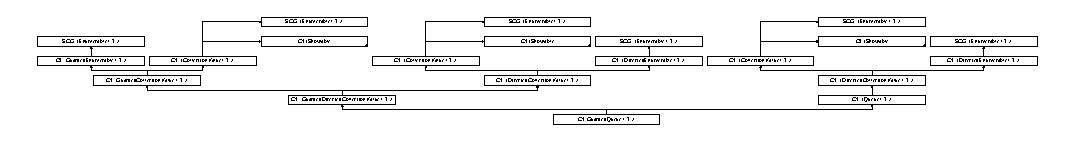
\includegraphics[height=1.441441cm]{class_c5_1_1_guarded_queue}
\end{center}
\end{figure}
\subsection*{Public Member Functions}
\begin{DoxyCompactItemize}
\item 
\hyperlink{class_c5_1_1_guarded_queue_ad8348b6d959ee703bf5b91b4885ae28f}{Guarded\+Queue} (\hyperlink{interface_c5_1_1_i_queue}{I\+Queue}$<$ T $>$ queue)
\begin{DoxyCompactList}\small\item\em Wrap a queue in a read-\/only wrapper \end{DoxyCompactList}\item 
void \hyperlink{class_c5_1_1_guarded_queue_af8b4a6e503df67d019015f2ccce7c06b}{Enqueue} (T item)
\item 
T \hyperlink{class_c5_1_1_guarded_queue_aeac8a6ef430740f2ec1df8346cd122a4}{Dequeue} ()
\end{DoxyCompactItemize}
\subsection*{Properties}
\begin{DoxyCompactItemize}
\item 
bool \hyperlink{class_c5_1_1_guarded_queue_a859d295a8e0e99348ddb273b88d33b15}{Allows\+Duplicates}\hspace{0.3cm}{\ttfamily  \mbox{[}get\mbox{]}}
\item 
T \hyperlink{class_c5_1_1_guarded_queue_a5c18da3f129993454969b145f1fce822}{this\mbox{[}int i\mbox{]}}\hspace{0.3cm}{\ttfamily  \mbox{[}get\mbox{]}}
\begin{DoxyCompactList}\small\item\em Index into the wrapped queue \end{DoxyCompactList}\end{DoxyCompactItemize}
\subsection*{Additional Inherited Members}


\subsection{Detailed Description}
A read-\/only wrapper for a generic indexable queue (allows indexing). 

Suitable for wrapping a T\+:\+C5.\+Circular\+Queue`1


\begin{DoxyTemplParams}{Template Parameters}
{\em T} & The item type.\\
\hline
\end{DoxyTemplParams}


\subsection{Constructor \& Destructor Documentation}
\hypertarget{class_c5_1_1_guarded_queue_ad8348b6d959ee703bf5b91b4885ae28f}{}\index{C5\+::\+Guarded\+Queue@{C5\+::\+Guarded\+Queue}!Guarded\+Queue@{Guarded\+Queue}}
\index{Guarded\+Queue@{Guarded\+Queue}!C5\+::\+Guarded\+Queue@{C5\+::\+Guarded\+Queue}}
\subsubsection[{Guarded\+Queue(\+I\+Queue$<$ T $>$ queue)}]{\setlength{\rightskip}{0pt plus 5cm}{\bf C5.\+Guarded\+Queue}$<$ T $>$.{\bf Guarded\+Queue} (
\begin{DoxyParamCaption}
\item[{{\bf I\+Queue}$<$ T $>$}]{queue}
\end{DoxyParamCaption}
)}\label{class_c5_1_1_guarded_queue_ad8348b6d959ee703bf5b91b4885ae28f}


Wrap a queue in a read-\/only wrapper 


\begin{DoxyParams}{Parameters}
{\em queue} & The queue\\
\hline
\end{DoxyParams}


\subsection{Member Function Documentation}
\hypertarget{class_c5_1_1_guarded_queue_aeac8a6ef430740f2ec1df8346cd122a4}{}\index{C5\+::\+Guarded\+Queue@{C5\+::\+Guarded\+Queue}!Dequeue@{Dequeue}}
\index{Dequeue@{Dequeue}!C5\+::\+Guarded\+Queue@{C5\+::\+Guarded\+Queue}}
\subsubsection[{Dequeue()}]{\setlength{\rightskip}{0pt plus 5cm}T {\bf C5.\+Guarded\+Queue}$<$ T $>$.Dequeue (
\begin{DoxyParamCaption}
{}
\end{DoxyParamCaption}
)}\label{class_c5_1_1_guarded_queue_aeac8a6ef430740f2ec1df8346cd122a4}





\begin{DoxyExceptions}{Exceptions}
{\em \hyperlink{class_c5_1_1_read_only_collection_exception}{Read\+Only\+Collection\+Exception}} & since this is a read-\/only wrappper\\
\hline
\end{DoxyExceptions}
\begin{DoxyReturn}{Returns}
-\/
\end{DoxyReturn}


Implements \hyperlink{interface_c5_1_1_i_queue_ae64bb24d3237ad9cef4f55593ca20bc7}{C5.\+I\+Queue$<$ T $>$}.

\hypertarget{class_c5_1_1_guarded_queue_af8b4a6e503df67d019015f2ccce7c06b}{}\index{C5\+::\+Guarded\+Queue@{C5\+::\+Guarded\+Queue}!Enqueue@{Enqueue}}
\index{Enqueue@{Enqueue}!C5\+::\+Guarded\+Queue@{C5\+::\+Guarded\+Queue}}
\subsubsection[{Enqueue(\+T item)}]{\setlength{\rightskip}{0pt plus 5cm}void {\bf C5.\+Guarded\+Queue}$<$ T $>$.Enqueue (
\begin{DoxyParamCaption}
\item[{T}]{item}
\end{DoxyParamCaption}
)}\label{class_c5_1_1_guarded_queue_af8b4a6e503df67d019015f2ccce7c06b}





\begin{DoxyExceptions}{Exceptions}
{\em \hyperlink{class_c5_1_1_read_only_collection_exception}{Read\+Only\+Collection\+Exception}} & since this is a read-\/only wrappper\\
\hline
\end{DoxyExceptions}
\begin{DoxyReturn}{Returns}
-\/
\end{DoxyReturn}


Implements \hyperlink{interface_c5_1_1_i_queue_afceb820ca32b996f6fd5c34a85ccbacd}{C5.\+I\+Queue$<$ T $>$}.



\subsection{Property Documentation}
\hypertarget{class_c5_1_1_guarded_queue_a859d295a8e0e99348ddb273b88d33b15}{}\index{C5\+::\+Guarded\+Queue@{C5\+::\+Guarded\+Queue}!Allows\+Duplicates@{Allows\+Duplicates}}
\index{Allows\+Duplicates@{Allows\+Duplicates}!C5\+::\+Guarded\+Queue@{C5\+::\+Guarded\+Queue}}
\subsubsection[{Allows\+Duplicates}]{\setlength{\rightskip}{0pt plus 5cm}bool {\bf C5.\+Guarded\+Queue}$<$ T $>$.Allows\+Duplicates\hspace{0.3cm}{\ttfamily [get]}}\label{class_c5_1_1_guarded_queue_a859d295a8e0e99348ddb273b88d33b15}




\hypertarget{class_c5_1_1_guarded_queue_a5c18da3f129993454969b145f1fce822}{}\index{C5\+::\+Guarded\+Queue@{C5\+::\+Guarded\+Queue}!this\mbox{[}int i\mbox{]}@{this[int i]}}
\index{this\mbox{[}int i\mbox{]}@{this[int i]}!C5\+::\+Guarded\+Queue@{C5\+::\+Guarded\+Queue}}
\subsubsection[{this[int i]}]{\setlength{\rightskip}{0pt plus 5cm}T {\bf C5.\+Guarded\+Queue}$<$ T $>$.this\mbox{[}int i\mbox{]}\hspace{0.3cm}{\ttfamily [get]}}\label{class_c5_1_1_guarded_queue_a5c18da3f129993454969b145f1fce822}


Index into the wrapped queue 


\begin{DoxyParams}{Parameters}
{\em i} & \\
\hline
\end{DoxyParams}
\begin{DoxyReturn}{Returns}

\end{DoxyReturn}


The documentation for this class was generated from the following file\+:\begin{DoxyCompactItemize}
\item 
C\+:/\+Users/rasmusl/\+Source/\+Repos/\+C5/\+C5/\hyperlink{_wrappers_8cs}{Wrappers.\+cs}\end{DoxyCompactItemize}

\hypertarget{class_c5_1_1_guarded_sequenced}{}\section{C5.\+Guarded\+Sequenced$<$ T $>$ Class Template Reference}
\label{class_c5_1_1_guarded_sequenced}\index{C5.\+Guarded\+Sequenced$<$ T $>$@{C5.\+Guarded\+Sequenced$<$ T $>$}}


A read-\/only wrapper for a sequenced collection  


Inheritance diagram for C5.\+Guarded\+Sequenced$<$ T $>$\+:\begin{figure}[H]
\begin{center}
\leavevmode
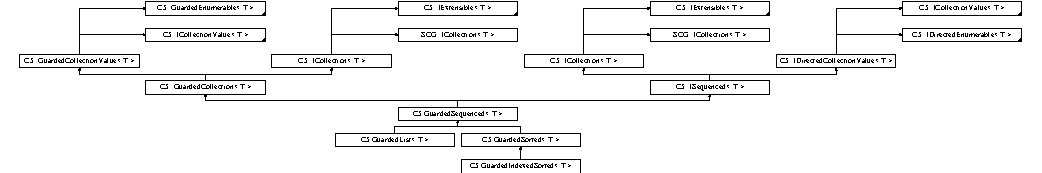
\includegraphics[height=2.300470cm]{class_c5_1_1_guarded_sequenced}
\end{center}
\end{figure}
\subsection*{Public Member Functions}
\begin{DoxyCompactItemize}
\item 
\hyperlink{class_c5_1_1_guarded_sequenced_ac95669006745b3cbd6499f705e943df9}{Guarded\+Sequenced} (\hyperlink{interface_c5_1_1_i_sequenced}{I\+Sequenced}$<$ T $>$ sorted)
\begin{DoxyCompactList}\small\item\em Wrap a sequenced collection in a read-\/only wrapper \end{DoxyCompactList}\item 
int \hyperlink{class_c5_1_1_guarded_sequenced_a610348d7c60a714f948a763ab5afc60d}{Find\+Index} (Func$<$ T, bool $>$ predicate)
\begin{DoxyCompactList}\small\item\em Check if there exists an item that satisfies a specific predicate in this collection and return the index of the first one. \end{DoxyCompactList}\item 
int \hyperlink{class_c5_1_1_guarded_sequenced_ad06df0c721132964b3f91c761232f74f}{Find\+Last\+Index} (Func$<$ T, bool $>$ predicate)
\begin{DoxyCompactList}\small\item\em Check if there exists an item that satisfies a specific predicate in this collection and return the index of the last one. \end{DoxyCompactList}\item 
int \hyperlink{class_c5_1_1_guarded_sequenced_a04214406cd7fe4814643b79c5005c799}{Get\+Sequenced\+Hash\+Code} ()
\item 
bool \hyperlink{class_c5_1_1_guarded_sequenced_ac4377e7ad77d3954865ad6500fb47245}{Sequenced\+Equals} (\hyperlink{interface_c5_1_1_i_sequenced}{I\+Sequenced}$<$ T $>$ that)
\item 
virtual \hyperlink{interface_c5_1_1_i_directed_collection_value}{I\+Directed\+Collection\+Value}$<$ T $>$ \hyperlink{class_c5_1_1_guarded_sequenced_a5bbddf444037001d526931116e6b16e7}{Backwards} ()
\begin{DoxyCompactList}\small\item\em Get a collection that enumerates the wrapped collection in the opposite direction \end{DoxyCompactList}\item 
virtual bool \hyperlink{class_c5_1_1_guarded_sequenced_a4741f8cd5c5fa8fb3d6b7a71268cdefb}{Find\+Last} (Func$<$ T, bool $>$ predicate, out T item)
\end{DoxyCompactItemize}
\subsection*{Properties}
\begin{DoxyCompactItemize}
\item 
\hyperlink{namespace_c5_aad282676794e49130eb8caed289395f8}{Enumeration\+Direction} \hyperlink{class_c5_1_1_guarded_sequenced_a252feee8e5260e42f03494c08dda6dc0}{Direction}\hspace{0.3cm}{\ttfamily  \mbox{[}get\mbox{]}}
\end{DoxyCompactItemize}
\subsection*{Additional Inherited Members}


\subsection{Detailed Description}
A read-\/only wrapper for a sequenced collection 

{\itshape This is mainly interesting as a base of other guard classes} 

\subsection{Constructor \& Destructor Documentation}
\hypertarget{class_c5_1_1_guarded_sequenced_ac95669006745b3cbd6499f705e943df9}{}\index{C5\+::\+Guarded\+Sequenced@{C5\+::\+Guarded\+Sequenced}!Guarded\+Sequenced@{Guarded\+Sequenced}}
\index{Guarded\+Sequenced@{Guarded\+Sequenced}!C5\+::\+Guarded\+Sequenced@{C5\+::\+Guarded\+Sequenced}}
\subsubsection[{Guarded\+Sequenced(\+I\+Sequenced$<$ T $>$ sorted)}]{\setlength{\rightskip}{0pt plus 5cm}{\bf C5.\+Guarded\+Sequenced}$<$ T $>$.{\bf Guarded\+Sequenced} (
\begin{DoxyParamCaption}
\item[{{\bf I\+Sequenced}$<$ T $>$}]{sorted}
\end{DoxyParamCaption}
)}\label{class_c5_1_1_guarded_sequenced_ac95669006745b3cbd6499f705e943df9}


Wrap a sequenced collection in a read-\/only wrapper 


\begin{DoxyParams}{Parameters}
{\em sorted} & \\
\hline
\end{DoxyParams}


\subsection{Member Function Documentation}
\hypertarget{class_c5_1_1_guarded_sequenced_a5bbddf444037001d526931116e6b16e7}{}\index{C5\+::\+Guarded\+Sequenced@{C5\+::\+Guarded\+Sequenced}!Backwards@{Backwards}}
\index{Backwards@{Backwards}!C5\+::\+Guarded\+Sequenced@{C5\+::\+Guarded\+Sequenced}}
\subsubsection[{Backwards()}]{\setlength{\rightskip}{0pt plus 5cm}virtual {\bf I\+Directed\+Collection\+Value}$<$T$>$ {\bf C5.\+Guarded\+Sequenced}$<$ T $>$.Backwards (
\begin{DoxyParamCaption}
{}
\end{DoxyParamCaption}
)\hspace{0.3cm}{\ttfamily [virtual]}}\label{class_c5_1_1_guarded_sequenced_a5bbddf444037001d526931116e6b16e7}


Get a collection that enumerates the wrapped collection in the opposite direction 

\begin{DoxyReturn}{Returns}
The mirrored collection
\end{DoxyReturn}


Implements \hyperlink{interface_c5_1_1_i_directed_collection_value_ae5665ed396ea2801266c4b2bfb3dae41}{C5.\+I\+Directed\+Collection\+Value$<$ T $>$}.

\hypertarget{class_c5_1_1_guarded_sequenced_a610348d7c60a714f948a763ab5afc60d}{}\index{C5\+::\+Guarded\+Sequenced@{C5\+::\+Guarded\+Sequenced}!Find\+Index@{Find\+Index}}
\index{Find\+Index@{Find\+Index}!C5\+::\+Guarded\+Sequenced@{C5\+::\+Guarded\+Sequenced}}
\subsubsection[{Find\+Index(\+Func$<$ T, bool $>$ predicate)}]{\setlength{\rightskip}{0pt plus 5cm}int {\bf C5.\+Guarded\+Sequenced}$<$ T $>$.Find\+Index (
\begin{DoxyParamCaption}
\item[{Func$<$ T, bool $>$}]{predicate}
\end{DoxyParamCaption}
)}\label{class_c5_1_1_guarded_sequenced_a610348d7c60a714f948a763ab5afc60d}


Check if there exists an item that satisfies a specific predicate in this collection and return the index of the first one. 


\begin{DoxyParams}{Parameters}
{\em predicate} & A delegate (T\+:\+Func`2 with 
\begin{DoxyCode}
R == \textcolor{keywordtype}{bool}
\end{DoxyCode}
) defining the predicate\\
\hline
\end{DoxyParams}
\begin{DoxyReturn}{Returns}
the index, if found, a negative value else
\end{DoxyReturn}
\hypertarget{class_c5_1_1_guarded_sequenced_a4741f8cd5c5fa8fb3d6b7a71268cdefb}{}\index{C5\+::\+Guarded\+Sequenced@{C5\+::\+Guarded\+Sequenced}!Find\+Last@{Find\+Last}}
\index{Find\+Last@{Find\+Last}!C5\+::\+Guarded\+Sequenced@{C5\+::\+Guarded\+Sequenced}}
\subsubsection[{Find\+Last(\+Func$<$ T, bool $>$ predicate, out T item)}]{\setlength{\rightskip}{0pt plus 5cm}virtual bool {\bf C5.\+Guarded\+Sequenced}$<$ T $>$.Find\+Last (
\begin{DoxyParamCaption}
\item[{Func$<$ T, bool $>$}]{predicate, }
\item[{out T}]{item}
\end{DoxyParamCaption}
)\hspace{0.3cm}{\ttfamily [virtual]}}\label{class_c5_1_1_guarded_sequenced_a4741f8cd5c5fa8fb3d6b7a71268cdefb}





\begin{DoxyParams}{Parameters}
{\em predicate} & \\
\hline
{\em item} & \\
\hline
\end{DoxyParams}
\begin{DoxyReturn}{Returns}

\end{DoxyReturn}


Implements \hyperlink{interface_c5_1_1_i_directed_collection_value_a93725b1f694e0d1cf5827e481ea467b7}{C5.\+I\+Directed\+Collection\+Value$<$ T $>$}.

\hypertarget{class_c5_1_1_guarded_sequenced_ad06df0c721132964b3f91c761232f74f}{}\index{C5\+::\+Guarded\+Sequenced@{C5\+::\+Guarded\+Sequenced}!Find\+Last\+Index@{Find\+Last\+Index}}
\index{Find\+Last\+Index@{Find\+Last\+Index}!C5\+::\+Guarded\+Sequenced@{C5\+::\+Guarded\+Sequenced}}
\subsubsection[{Find\+Last\+Index(\+Func$<$ T, bool $>$ predicate)}]{\setlength{\rightskip}{0pt plus 5cm}int {\bf C5.\+Guarded\+Sequenced}$<$ T $>$.Find\+Last\+Index (
\begin{DoxyParamCaption}
\item[{Func$<$ T, bool $>$}]{predicate}
\end{DoxyParamCaption}
)}\label{class_c5_1_1_guarded_sequenced_ad06df0c721132964b3f91c761232f74f}


Check if there exists an item that satisfies a specific predicate in this collection and return the index of the last one. 


\begin{DoxyParams}{Parameters}
{\em predicate} & A delegate (T\+:\+Func`2 with 
\begin{DoxyCode}
R == \textcolor{keywordtype}{bool}
\end{DoxyCode}
) defining the predicate\\
\hline
\end{DoxyParams}
\begin{DoxyReturn}{Returns}
the index, if found, a negative value else
\end{DoxyReturn}
\hypertarget{class_c5_1_1_guarded_sequenced_a04214406cd7fe4814643b79c5005c799}{}\index{C5\+::\+Guarded\+Sequenced@{C5\+::\+Guarded\+Sequenced}!Get\+Sequenced\+Hash\+Code@{Get\+Sequenced\+Hash\+Code}}
\index{Get\+Sequenced\+Hash\+Code@{Get\+Sequenced\+Hash\+Code}!C5\+::\+Guarded\+Sequenced@{C5\+::\+Guarded\+Sequenced}}
\subsubsection[{Get\+Sequenced\+Hash\+Code()}]{\setlength{\rightskip}{0pt plus 5cm}int {\bf C5.\+Guarded\+Sequenced}$<$ T $>$.Get\+Sequenced\+Hash\+Code (
\begin{DoxyParamCaption}
{}
\end{DoxyParamCaption}
)}\label{class_c5_1_1_guarded_sequenced_a04214406cd7fe4814643b79c5005c799}




\begin{DoxyReturn}{Returns}

\end{DoxyReturn}


Implements \hyperlink{interface_c5_1_1_i_sequenced_afb06eeccff646bb763c76c1826b177fe}{C5.\+I\+Sequenced$<$ T $>$}.

\hypertarget{class_c5_1_1_guarded_sequenced_ac4377e7ad77d3954865ad6500fb47245}{}\index{C5\+::\+Guarded\+Sequenced@{C5\+::\+Guarded\+Sequenced}!Sequenced\+Equals@{Sequenced\+Equals}}
\index{Sequenced\+Equals@{Sequenced\+Equals}!C5\+::\+Guarded\+Sequenced@{C5\+::\+Guarded\+Sequenced}}
\subsubsection[{Sequenced\+Equals(\+I\+Sequenced$<$ T $>$ that)}]{\setlength{\rightskip}{0pt plus 5cm}bool {\bf C5.\+Guarded\+Sequenced}$<$ T $>$.Sequenced\+Equals (
\begin{DoxyParamCaption}
\item[{{\bf I\+Sequenced}$<$ T $>$}]{that}
\end{DoxyParamCaption}
)}\label{class_c5_1_1_guarded_sequenced_ac4377e7ad77d3954865ad6500fb47245}





\begin{DoxyParams}{Parameters}
{\em that} & \\
\hline
\end{DoxyParams}
\begin{DoxyReturn}{Returns}

\end{DoxyReturn}


Implements \hyperlink{interface_c5_1_1_i_sequenced_aeb2be77c5c30ab10f468222f6cbb795f}{C5.\+I\+Sequenced$<$ T $>$}.



\subsection{Property Documentation}
\hypertarget{class_c5_1_1_guarded_sequenced_a252feee8e5260e42f03494c08dda6dc0}{}\index{C5\+::\+Guarded\+Sequenced@{C5\+::\+Guarded\+Sequenced}!Direction@{Direction}}
\index{Direction@{Direction}!C5\+::\+Guarded\+Sequenced@{C5\+::\+Guarded\+Sequenced}}
\subsubsection[{Direction}]{\setlength{\rightskip}{0pt plus 5cm}{\bf Enumeration\+Direction} {\bf C5.\+Guarded\+Sequenced}$<$ T $>$.Direction\hspace{0.3cm}{\ttfamily [get]}}\label{class_c5_1_1_guarded_sequenced_a252feee8e5260e42f03494c08dda6dc0}




{\ttfamily Forwards} if same, else {\ttfamily Backwards} 

The enumeration direction relative to the original collection.

The documentation for this class was generated from the following file\+:\begin{DoxyCompactItemize}
\item 
C\+:/\+Users/rasmusl/\+Source/\+Repos/\+C5/\+C5/\hyperlink{_wrappers_8cs}{Wrappers.\+cs}\end{DoxyCompactItemize}

\hypertarget{class_c5_1_1_guarded_sorted}{}\section{C5.\+Guarded\+Sorted$<$ T $>$ Class Template Reference}
\label{class_c5_1_1_guarded_sorted}\index{C5.\+Guarded\+Sorted$<$ T $>$@{C5.\+Guarded\+Sorted$<$ T $>$}}


A read-\/only wrapper for a sorted collection  


Inheritance diagram for C5.\+Guarded\+Sorted$<$ T $>$\+:\begin{figure}[H]
\begin{center}
\leavevmode
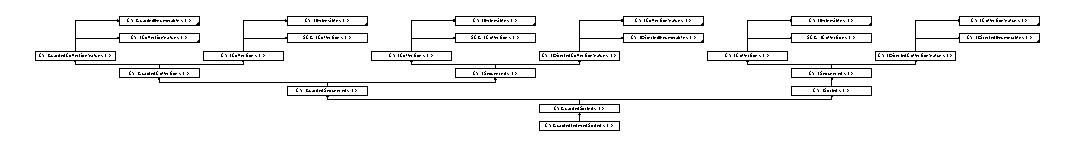
\includegraphics[height=1.533646cm]{class_c5_1_1_guarded_sorted}
\end{center}
\end{figure}
\subsection*{Public Member Functions}
\begin{DoxyCompactItemize}
\item 
\hyperlink{class_c5_1_1_guarded_sorted_a83a43467e2f40a5d7994c165df409c9d}{Guarded\+Sorted} (\hyperlink{interface_c5_1_1_i_sorted}{I\+Sorted}$<$ T $>$ sorted)
\begin{DoxyCompactList}\small\item\em Wrap a sorted collection in a read-\/only wrapper \end{DoxyCompactList}\item 
bool \hyperlink{class_c5_1_1_guarded_sorted_a5d51f1d79c4ad4c84684f6102562d44a}{Try\+Predecessor} (T item, out T res)
\begin{DoxyCompactList}\small\item\em Find the strict predecessor of item in the guarded sorted collection, that is, the greatest item in the collection smaller than the item. \end{DoxyCompactList}\item 
bool \hyperlink{class_c5_1_1_guarded_sorted_a7a8a2a146dc48c07818e434f14473dac}{Try\+Successor} (T item, out T res)
\begin{DoxyCompactList}\small\item\em Find the strict successor of item in the guarded sorted collection, that is, the least item in the collection greater than the supplied value. \end{DoxyCompactList}\item 
bool \hyperlink{class_c5_1_1_guarded_sorted_ac0895c0ec8adf94a479c0a22b337b122}{Try\+Weak\+Predecessor} (T item, out T res)
\begin{DoxyCompactList}\small\item\em Find the weak predecessor of item in the guarded sorted collection, that is, the greatest item in the collection smaller than or equal to the item. \end{DoxyCompactList}\item 
bool \hyperlink{class_c5_1_1_guarded_sorted_a0f00bb7238c3bc374aa085205448f533}{Try\+Weak\+Successor} (T item, out T res)
\begin{DoxyCompactList}\small\item\em Find the weak successor of item in the sorted collection, that is, the least item in the collection greater than or equal to the supplied value. \end{DoxyCompactList}\item 
T \hyperlink{class_c5_1_1_guarded_sorted_afd96c13a6d58d8db800b8ba78f843e29}{Predecessor} (T item)
\begin{DoxyCompactList}\small\item\em Find the predecessor of the item in the wrapped sorted collection \end{DoxyCompactList}\item 
T \hyperlink{class_c5_1_1_guarded_sorted_a042b2d69142f8957f0fec4958e67a99a}{Successor} (T item)
\begin{DoxyCompactList}\small\item\em Find the Successor of the item in the wrapped sorted collection \end{DoxyCompactList}\item 
T \hyperlink{class_c5_1_1_guarded_sorted_ae5fed4839e2e079fc0c07e141c7b51e3}{Weak\+Predecessor} (T item)
\begin{DoxyCompactList}\small\item\em Find the weak predecessor of the item in the wrapped sorted collection \end{DoxyCompactList}\item 
T \hyperlink{class_c5_1_1_guarded_sorted_a6a3aeb46c7bf83990651ce69a53f9fc6}{Weak\+Successor} (T item)
\begin{DoxyCompactList}\small\item\em Find the weak Successor of the item in the wrapped sorted collection \end{DoxyCompactList}\item 
bool \hyperlink{class_c5_1_1_guarded_sorted_a0372f6f2e220c389973eea8201390a27}{Cut} (I\+Comparable$<$ T $>$ c, out T low, out bool lval, out T high, out bool hval)
\begin{DoxyCompactList}\small\item\em Run Cut on the wrapped sorted collection \end{DoxyCompactList}\item 
\hyperlink{interface_c5_1_1_i_directed_enumerable}{I\+Directed\+Enumerable}$<$ T $>$ \hyperlink{class_c5_1_1_guarded_sorted_ac163fd0c999d9bd1581a2313c716b573}{Range\+From} (T bot)
\begin{DoxyCompactList}\small\item\em Get the specified range from the wrapped collection. (The current implementation erroneously does not wrap the result.) \end{DoxyCompactList}\item 
\hyperlink{interface_c5_1_1_i_directed_enumerable}{I\+Directed\+Enumerable}$<$ T $>$ \hyperlink{class_c5_1_1_guarded_sorted_a4654fa234e549063c0a820662e6b8e9e}{Range\+From\+To} (T bot, T top)
\begin{DoxyCompactList}\small\item\em Get the specified range from the wrapped collection. (The current implementation erroneously does not wrap the result.) \end{DoxyCompactList}\item 
\hyperlink{interface_c5_1_1_i_directed_enumerable}{I\+Directed\+Enumerable}$<$ T $>$ \hyperlink{class_c5_1_1_guarded_sorted_a21305628969a9beaa6e0f0d06fb171a6}{Range\+To} (T top)
\begin{DoxyCompactList}\small\item\em Get the specified range from the wrapped collection. (The current implementation erroneously does not wrap the result.) \end{DoxyCompactList}\item 
\hyperlink{interface_c5_1_1_i_directed_collection_value}{I\+Directed\+Collection\+Value}$<$ T $>$ \hyperlink{class_c5_1_1_guarded_sorted_a810e407c33bdf337c32ceb9c2d9773ad}{Range\+All} ()
\begin{DoxyCompactList}\small\item\em Get the specified range from the wrapped collection. (The current implementation erroneously does not wrap the result.) \end{DoxyCompactList}\item 
void \hyperlink{class_c5_1_1_guarded_sorted_a5dfe71d83337e50a8d38002c7836680d}{Add\+Sorted} (S\+C\+G.\+I\+Enumerable$<$ T $>$ items)
\item 
void \hyperlink{class_c5_1_1_guarded_sorted_a50fb581a7fdc2aa8565fb7aeeccd4cd1}{Remove\+Range\+From} (T low)
\item 
void \hyperlink{class_c5_1_1_guarded_sorted_aa778f695d7e887a7ca4672ccdd06a689}{Remove\+Range\+From\+To} (T low, T hi)
\item 
void \hyperlink{class_c5_1_1_guarded_sorted_a913a700b2bdd5fb9582c818360468c3a}{Remove\+Range\+To} (T hi)
\item 
T \hyperlink{class_c5_1_1_guarded_sorted_a74fbcdd950a8673bc61e09539470748a}{Find\+Min} ()
\begin{DoxyCompactList}\small\item\em Find the minimum of the wrapped collection \end{DoxyCompactList}\item 
T \hyperlink{class_c5_1_1_guarded_sorted_a7cc91f7815ef8e6e43006289e0ab7305}{Delete\+Min} ()
\item 
T \hyperlink{class_c5_1_1_guarded_sorted_ab6f7371f2bdec615b28c075493ef70d8}{Find\+Max} ()
\begin{DoxyCompactList}\small\item\em Find the maximum of the wrapped collection \end{DoxyCompactList}\item 
T \hyperlink{class_c5_1_1_guarded_sorted_a24f97b59e6d0e9efb7cc7be97f739cd5}{Delete\+Max} ()
\end{DoxyCompactItemize}
\subsection*{Properties}
\begin{DoxyCompactItemize}
\item 
S\+C\+G.\+I\+Comparer$<$ T $>$ \hyperlink{class_c5_1_1_guarded_sorted_a189be757a095db06b38471bfa2d67903}{Comparer}\hspace{0.3cm}{\ttfamily  \mbox{[}get\mbox{]}}
\begin{DoxyCompactList}\small\item\em The comparer object supplied at creation time for the underlying collection \end{DoxyCompactList}\end{DoxyCompactItemize}
\subsection*{Additional Inherited Members}


\subsection{Detailed Description}
A read-\/only wrapper for a sorted collection 

{\itshape This is mainly interesting as a base of other guard classes} 

\subsection{Constructor \& Destructor Documentation}
\hypertarget{class_c5_1_1_guarded_sorted_a83a43467e2f40a5d7994c165df409c9d}{}\index{C5\+::\+Guarded\+Sorted@{C5\+::\+Guarded\+Sorted}!Guarded\+Sorted@{Guarded\+Sorted}}
\index{Guarded\+Sorted@{Guarded\+Sorted}!C5\+::\+Guarded\+Sorted@{C5\+::\+Guarded\+Sorted}}
\subsubsection[{Guarded\+Sorted(\+I\+Sorted$<$ T $>$ sorted)}]{\setlength{\rightskip}{0pt plus 5cm}{\bf C5.\+Guarded\+Sorted}$<$ T $>$.{\bf Guarded\+Sorted} (
\begin{DoxyParamCaption}
\item[{{\bf I\+Sorted}$<$ T $>$}]{sorted}
\end{DoxyParamCaption}
)}\label{class_c5_1_1_guarded_sorted_a83a43467e2f40a5d7994c165df409c9d}


Wrap a sorted collection in a read-\/only wrapper 


\begin{DoxyParams}{Parameters}
{\em sorted} & \\
\hline
\end{DoxyParams}


\subsection{Member Function Documentation}
\hypertarget{class_c5_1_1_guarded_sorted_a5dfe71d83337e50a8d38002c7836680d}{}\index{C5\+::\+Guarded\+Sorted@{C5\+::\+Guarded\+Sorted}!Add\+Sorted@{Add\+Sorted}}
\index{Add\+Sorted@{Add\+Sorted}!C5\+::\+Guarded\+Sorted@{C5\+::\+Guarded\+Sorted}}
\subsubsection[{Add\+Sorted(\+S\+C\+G.\+I\+Enumerable$<$ T $>$ items)}]{\setlength{\rightskip}{0pt plus 5cm}void {\bf C5.\+Guarded\+Sorted}$<$ T $>$.Add\+Sorted (
\begin{DoxyParamCaption}
\item[{S\+C\+G.\+I\+Enumerable$<$ T $>$}]{items}
\end{DoxyParamCaption}
)}\label{class_c5_1_1_guarded_sorted_a5dfe71d83337e50a8d38002c7836680d}





\begin{DoxyExceptions}{Exceptions}
{\em \hyperlink{class_c5_1_1_read_only_collection_exception}{Read\+Only\+Collection\+Exception}} & since this is a read-\/only wrappper\\
\hline
\end{DoxyExceptions}

\begin{DoxyParams}{Parameters}
{\em items} & \\
\hline
\end{DoxyParams}


Implements \hyperlink{interface_c5_1_1_i_sorted_a51dd21143c9438dc9f841a9d7b6f6b3f}{C5.\+I\+Sorted$<$ T $>$}.

\hypertarget{class_c5_1_1_guarded_sorted_a0372f6f2e220c389973eea8201390a27}{}\index{C5\+::\+Guarded\+Sorted@{C5\+::\+Guarded\+Sorted}!Cut@{Cut}}
\index{Cut@{Cut}!C5\+::\+Guarded\+Sorted@{C5\+::\+Guarded\+Sorted}}
\subsubsection[{Cut(\+I\+Comparable$<$ T $>$ c, out T low, out bool lval, out T high, out bool hval)}]{\setlength{\rightskip}{0pt plus 5cm}bool {\bf C5.\+Guarded\+Sorted}$<$ T $>$.Cut (
\begin{DoxyParamCaption}
\item[{I\+Comparable$<$ T $>$}]{c, }
\item[{out T}]{low, }
\item[{out bool}]{lval, }
\item[{out T}]{high, }
\item[{out bool}]{hval}
\end{DoxyParamCaption}
)}\label{class_c5_1_1_guarded_sorted_a0372f6f2e220c389973eea8201390a27}


Run Cut on the wrapped sorted collection 


\begin{DoxyParams}{Parameters}
{\em c} & \\
\hline
{\em low} & \\
\hline
{\em lval} & \\
\hline
{\em high} & \\
\hline
{\em hval} & \\
\hline
\end{DoxyParams}
\begin{DoxyReturn}{Returns}

\end{DoxyReturn}


Implements \hyperlink{interface_c5_1_1_i_sorted_a7acdf0ef5765c2554e5efa8df856c2b4}{C5.\+I\+Sorted$<$ T $>$}.

\hypertarget{class_c5_1_1_guarded_sorted_a24f97b59e6d0e9efb7cc7be97f739cd5}{}\index{C5\+::\+Guarded\+Sorted@{C5\+::\+Guarded\+Sorted}!Delete\+Max@{Delete\+Max}}
\index{Delete\+Max@{Delete\+Max}!C5\+::\+Guarded\+Sorted@{C5\+::\+Guarded\+Sorted}}
\subsubsection[{Delete\+Max()}]{\setlength{\rightskip}{0pt plus 5cm}T {\bf C5.\+Guarded\+Sorted}$<$ T $>$.Delete\+Max (
\begin{DoxyParamCaption}
{}
\end{DoxyParamCaption}
)}\label{class_c5_1_1_guarded_sorted_a24f97b59e6d0e9efb7cc7be97f739cd5}





\begin{DoxyExceptions}{Exceptions}
{\em \hyperlink{class_c5_1_1_read_only_collection_exception}{Read\+Only\+Collection\+Exception}} & since this is a read-\/only wrappper\\
\hline
\end{DoxyExceptions}
\begin{DoxyReturn}{Returns}

\end{DoxyReturn}


Implements \hyperlink{interface_c5_1_1_i_sorted_a58b26b758745ad2146252b9e5ff2965b}{C5.\+I\+Sorted$<$ T $>$}.

\hypertarget{class_c5_1_1_guarded_sorted_a7cc91f7815ef8e6e43006289e0ab7305}{}\index{C5\+::\+Guarded\+Sorted@{C5\+::\+Guarded\+Sorted}!Delete\+Min@{Delete\+Min}}
\index{Delete\+Min@{Delete\+Min}!C5\+::\+Guarded\+Sorted@{C5\+::\+Guarded\+Sorted}}
\subsubsection[{Delete\+Min()}]{\setlength{\rightskip}{0pt plus 5cm}T {\bf C5.\+Guarded\+Sorted}$<$ T $>$.Delete\+Min (
\begin{DoxyParamCaption}
{}
\end{DoxyParamCaption}
)}\label{class_c5_1_1_guarded_sorted_a7cc91f7815ef8e6e43006289e0ab7305}





\begin{DoxyExceptions}{Exceptions}
{\em \hyperlink{class_c5_1_1_read_only_collection_exception}{Read\+Only\+Collection\+Exception}} & since this is a read-\/only wrappper\\
\hline
\end{DoxyExceptions}
\begin{DoxyReturn}{Returns}

\end{DoxyReturn}


Implements \hyperlink{interface_c5_1_1_i_sorted_ad30bc55d0c81e695896d459422b76954}{C5.\+I\+Sorted$<$ T $>$}.

\hypertarget{class_c5_1_1_guarded_sorted_ab6f7371f2bdec615b28c075493ef70d8}{}\index{C5\+::\+Guarded\+Sorted@{C5\+::\+Guarded\+Sorted}!Find\+Max@{Find\+Max}}
\index{Find\+Max@{Find\+Max}!C5\+::\+Guarded\+Sorted@{C5\+::\+Guarded\+Sorted}}
\subsubsection[{Find\+Max()}]{\setlength{\rightskip}{0pt plus 5cm}T {\bf C5.\+Guarded\+Sorted}$<$ T $>$.Find\+Max (
\begin{DoxyParamCaption}
{}
\end{DoxyParamCaption}
)}\label{class_c5_1_1_guarded_sorted_ab6f7371f2bdec615b28c075493ef70d8}


Find the maximum of the wrapped collection 

\begin{DoxyReturn}{Returns}
The maximum
\end{DoxyReturn}


Implements \hyperlink{interface_c5_1_1_i_sorted_a9321a921a443cfd8411534fbef19ab00}{C5.\+I\+Sorted$<$ T $>$}.

\hypertarget{class_c5_1_1_guarded_sorted_a74fbcdd950a8673bc61e09539470748a}{}\index{C5\+::\+Guarded\+Sorted@{C5\+::\+Guarded\+Sorted}!Find\+Min@{Find\+Min}}
\index{Find\+Min@{Find\+Min}!C5\+::\+Guarded\+Sorted@{C5\+::\+Guarded\+Sorted}}
\subsubsection[{Find\+Min()}]{\setlength{\rightskip}{0pt plus 5cm}T {\bf C5.\+Guarded\+Sorted}$<$ T $>$.Find\+Min (
\begin{DoxyParamCaption}
{}
\end{DoxyParamCaption}
)}\label{class_c5_1_1_guarded_sorted_a74fbcdd950a8673bc61e09539470748a}


Find the minimum of the wrapped collection 

\begin{DoxyReturn}{Returns}
The minimum
\end{DoxyReturn}


Implements \hyperlink{interface_c5_1_1_i_sorted_ad7a7fc9df9ff4fd5e5ab399c5703f995}{C5.\+I\+Sorted$<$ T $>$}.

\hypertarget{class_c5_1_1_guarded_sorted_afd96c13a6d58d8db800b8ba78f843e29}{}\index{C5\+::\+Guarded\+Sorted@{C5\+::\+Guarded\+Sorted}!Predecessor@{Predecessor}}
\index{Predecessor@{Predecessor}!C5\+::\+Guarded\+Sorted@{C5\+::\+Guarded\+Sorted}}
\subsubsection[{Predecessor(\+T item)}]{\setlength{\rightskip}{0pt plus 5cm}T {\bf C5.\+Guarded\+Sorted}$<$ T $>$.Predecessor (
\begin{DoxyParamCaption}
\item[{T}]{item}
\end{DoxyParamCaption}
)}\label{class_c5_1_1_guarded_sorted_afd96c13a6d58d8db800b8ba78f843e29}


Find the predecessor of the item in the wrapped sorted collection 


\begin{DoxyExceptions}{Exceptions}
{\em \hyperlink{class_c5_1_1_no_such_item_exception}{No\+Such\+Item\+Exception}} & if no such element exists \\
\hline
\end{DoxyExceptions}

\begin{DoxyParams}{Parameters}
{\em item} & The item\\
\hline
\end{DoxyParams}
\begin{DoxyReturn}{Returns}
The predecessor
\end{DoxyReturn}


Implements \hyperlink{interface_c5_1_1_i_sorted_a973bf071df358a008bdfed289a38ff71}{C5.\+I\+Sorted$<$ T $>$}.

\hypertarget{class_c5_1_1_guarded_sorted_a810e407c33bdf337c32ceb9c2d9773ad}{}\index{C5\+::\+Guarded\+Sorted@{C5\+::\+Guarded\+Sorted}!Range\+All@{Range\+All}}
\index{Range\+All@{Range\+All}!C5\+::\+Guarded\+Sorted@{C5\+::\+Guarded\+Sorted}}
\subsubsection[{Range\+All()}]{\setlength{\rightskip}{0pt plus 5cm}{\bf I\+Directed\+Collection\+Value}$<$T$>$ {\bf C5.\+Guarded\+Sorted}$<$ T $>$.Range\+All (
\begin{DoxyParamCaption}
{}
\end{DoxyParamCaption}
)}\label{class_c5_1_1_guarded_sorted_a810e407c33bdf337c32ceb9c2d9773ad}


Get the specified range from the wrapped collection. (The current implementation erroneously does not wrap the result.) 

\begin{DoxyReturn}{Returns}

\end{DoxyReturn}


Implements \hyperlink{interface_c5_1_1_i_sorted_ad90021b06a8976cc8c043104cf8e1ca4}{C5.\+I\+Sorted$<$ T $>$}.

\hypertarget{class_c5_1_1_guarded_sorted_ac163fd0c999d9bd1581a2313c716b573}{}\index{C5\+::\+Guarded\+Sorted@{C5\+::\+Guarded\+Sorted}!Range\+From@{Range\+From}}
\index{Range\+From@{Range\+From}!C5\+::\+Guarded\+Sorted@{C5\+::\+Guarded\+Sorted}}
\subsubsection[{Range\+From(\+T bot)}]{\setlength{\rightskip}{0pt plus 5cm}{\bf I\+Directed\+Enumerable}$<$T$>$ {\bf C5.\+Guarded\+Sorted}$<$ T $>$.Range\+From (
\begin{DoxyParamCaption}
\item[{T}]{bot}
\end{DoxyParamCaption}
)}\label{class_c5_1_1_guarded_sorted_ac163fd0c999d9bd1581a2313c716b573}


Get the specified range from the wrapped collection. (The current implementation erroneously does not wrap the result.) 


\begin{DoxyParams}{Parameters}
{\em bot} & \\
\hline
\end{DoxyParams}
\begin{DoxyReturn}{Returns}

\end{DoxyReturn}


Implements \hyperlink{interface_c5_1_1_i_sorted_a0eabf2b7418467cf0ee1cfb15b6b9e34}{C5.\+I\+Sorted$<$ T $>$}.

\hypertarget{class_c5_1_1_guarded_sorted_a4654fa234e549063c0a820662e6b8e9e}{}\index{C5\+::\+Guarded\+Sorted@{C5\+::\+Guarded\+Sorted}!Range\+From\+To@{Range\+From\+To}}
\index{Range\+From\+To@{Range\+From\+To}!C5\+::\+Guarded\+Sorted@{C5\+::\+Guarded\+Sorted}}
\subsubsection[{Range\+From\+To(\+T bot, T top)}]{\setlength{\rightskip}{0pt plus 5cm}{\bf I\+Directed\+Enumerable}$<$T$>$ {\bf C5.\+Guarded\+Sorted}$<$ T $>$.Range\+From\+To (
\begin{DoxyParamCaption}
\item[{T}]{bot, }
\item[{T}]{top}
\end{DoxyParamCaption}
)}\label{class_c5_1_1_guarded_sorted_a4654fa234e549063c0a820662e6b8e9e}


Get the specified range from the wrapped collection. (The current implementation erroneously does not wrap the result.) 


\begin{DoxyParams}{Parameters}
{\em bot} & \\
\hline
{\em top} & \\
\hline
\end{DoxyParams}
\begin{DoxyReturn}{Returns}

\end{DoxyReturn}


Implements \hyperlink{interface_c5_1_1_i_sorted_a66a3e2a57ca820b3a67b2f8d99e3c7cb}{C5.\+I\+Sorted$<$ T $>$}.

\hypertarget{class_c5_1_1_guarded_sorted_a21305628969a9beaa6e0f0d06fb171a6}{}\index{C5\+::\+Guarded\+Sorted@{C5\+::\+Guarded\+Sorted}!Range\+To@{Range\+To}}
\index{Range\+To@{Range\+To}!C5\+::\+Guarded\+Sorted@{C5\+::\+Guarded\+Sorted}}
\subsubsection[{Range\+To(\+T top)}]{\setlength{\rightskip}{0pt plus 5cm}{\bf I\+Directed\+Enumerable}$<$T$>$ {\bf C5.\+Guarded\+Sorted}$<$ T $>$.Range\+To (
\begin{DoxyParamCaption}
\item[{T}]{top}
\end{DoxyParamCaption}
)}\label{class_c5_1_1_guarded_sorted_a21305628969a9beaa6e0f0d06fb171a6}


Get the specified range from the wrapped collection. (The current implementation erroneously does not wrap the result.) 


\begin{DoxyParams}{Parameters}
{\em top} & \\
\hline
\end{DoxyParams}
\begin{DoxyReturn}{Returns}

\end{DoxyReturn}


Implements \hyperlink{interface_c5_1_1_i_sorted_a438ee04db17957587e7651f4c010814a}{C5.\+I\+Sorted$<$ T $>$}.

\hypertarget{class_c5_1_1_guarded_sorted_a50fb581a7fdc2aa8565fb7aeeccd4cd1}{}\index{C5\+::\+Guarded\+Sorted@{C5\+::\+Guarded\+Sorted}!Remove\+Range\+From@{Remove\+Range\+From}}
\index{Remove\+Range\+From@{Remove\+Range\+From}!C5\+::\+Guarded\+Sorted@{C5\+::\+Guarded\+Sorted}}
\subsubsection[{Remove\+Range\+From(\+T low)}]{\setlength{\rightskip}{0pt plus 5cm}void {\bf C5.\+Guarded\+Sorted}$<$ T $>$.Remove\+Range\+From (
\begin{DoxyParamCaption}
\item[{T}]{low}
\end{DoxyParamCaption}
)}\label{class_c5_1_1_guarded_sorted_a50fb581a7fdc2aa8565fb7aeeccd4cd1}





\begin{DoxyExceptions}{Exceptions}
{\em \hyperlink{class_c5_1_1_read_only_collection_exception}{Read\+Only\+Collection\+Exception}} & since this is a read-\/only wrappper\\
\hline
\end{DoxyExceptions}

\begin{DoxyParams}{Parameters}
{\em low} & \\
\hline
\end{DoxyParams}


Implements \hyperlink{interface_c5_1_1_i_sorted_ab6f6647d63da58ce3b6d837fd73ff0a1}{C5.\+I\+Sorted$<$ T $>$}.

\hypertarget{class_c5_1_1_guarded_sorted_aa778f695d7e887a7ca4672ccdd06a689}{}\index{C5\+::\+Guarded\+Sorted@{C5\+::\+Guarded\+Sorted}!Remove\+Range\+From\+To@{Remove\+Range\+From\+To}}
\index{Remove\+Range\+From\+To@{Remove\+Range\+From\+To}!C5\+::\+Guarded\+Sorted@{C5\+::\+Guarded\+Sorted}}
\subsubsection[{Remove\+Range\+From\+To(\+T low, T hi)}]{\setlength{\rightskip}{0pt plus 5cm}void {\bf C5.\+Guarded\+Sorted}$<$ T $>$.Remove\+Range\+From\+To (
\begin{DoxyParamCaption}
\item[{T}]{low, }
\item[{T}]{hi}
\end{DoxyParamCaption}
)}\label{class_c5_1_1_guarded_sorted_aa778f695d7e887a7ca4672ccdd06a689}





\begin{DoxyExceptions}{Exceptions}
{\em \hyperlink{class_c5_1_1_read_only_collection_exception}{Read\+Only\+Collection\+Exception}} & since this is a read-\/only wrappper\\
\hline
\end{DoxyExceptions}

\begin{DoxyParams}{Parameters}
{\em low} & \\
\hline
{\em hi} & \\
\hline
\end{DoxyParams}


Implements \hyperlink{interface_c5_1_1_i_sorted_a3d2125d5a4b4c5ce0fb34fcb8be0fa72}{C5.\+I\+Sorted$<$ T $>$}.

\hypertarget{class_c5_1_1_guarded_sorted_a913a700b2bdd5fb9582c818360468c3a}{}\index{C5\+::\+Guarded\+Sorted@{C5\+::\+Guarded\+Sorted}!Remove\+Range\+To@{Remove\+Range\+To}}
\index{Remove\+Range\+To@{Remove\+Range\+To}!C5\+::\+Guarded\+Sorted@{C5\+::\+Guarded\+Sorted}}
\subsubsection[{Remove\+Range\+To(\+T hi)}]{\setlength{\rightskip}{0pt plus 5cm}void {\bf C5.\+Guarded\+Sorted}$<$ T $>$.Remove\+Range\+To (
\begin{DoxyParamCaption}
\item[{T}]{hi}
\end{DoxyParamCaption}
)}\label{class_c5_1_1_guarded_sorted_a913a700b2bdd5fb9582c818360468c3a}





\begin{DoxyExceptions}{Exceptions}
{\em \hyperlink{class_c5_1_1_read_only_collection_exception}{Read\+Only\+Collection\+Exception}} & since this is a read-\/only wrappper\\
\hline
\end{DoxyExceptions}

\begin{DoxyParams}{Parameters}
{\em hi} & \\
\hline
\end{DoxyParams}


Implements \hyperlink{interface_c5_1_1_i_sorted_ad2e5ddc9c56ecf42340571bdfabf5d22}{C5.\+I\+Sorted$<$ T $>$}.

\hypertarget{class_c5_1_1_guarded_sorted_a042b2d69142f8957f0fec4958e67a99a}{}\index{C5\+::\+Guarded\+Sorted@{C5\+::\+Guarded\+Sorted}!Successor@{Successor}}
\index{Successor@{Successor}!C5\+::\+Guarded\+Sorted@{C5\+::\+Guarded\+Sorted}}
\subsubsection[{Successor(\+T item)}]{\setlength{\rightskip}{0pt plus 5cm}T {\bf C5.\+Guarded\+Sorted}$<$ T $>$.Successor (
\begin{DoxyParamCaption}
\item[{T}]{item}
\end{DoxyParamCaption}
)}\label{class_c5_1_1_guarded_sorted_a042b2d69142f8957f0fec4958e67a99a}


Find the Successor of the item in the wrapped sorted collection 


\begin{DoxyExceptions}{Exceptions}
{\em \hyperlink{class_c5_1_1_no_such_item_exception}{No\+Such\+Item\+Exception}} & if no such element exists \\
\hline
\end{DoxyExceptions}

\begin{DoxyParams}{Parameters}
{\em item} & The item\\
\hline
\end{DoxyParams}
\begin{DoxyReturn}{Returns}
The Successor
\end{DoxyReturn}


Implements \hyperlink{interface_c5_1_1_i_sorted_a6620b9769f5125157e254d8077744515}{C5.\+I\+Sorted$<$ T $>$}.

\hypertarget{class_c5_1_1_guarded_sorted_a5d51f1d79c4ad4c84684f6102562d44a}{}\index{C5\+::\+Guarded\+Sorted@{C5\+::\+Guarded\+Sorted}!Try\+Predecessor@{Try\+Predecessor}}
\index{Try\+Predecessor@{Try\+Predecessor}!C5\+::\+Guarded\+Sorted@{C5\+::\+Guarded\+Sorted}}
\subsubsection[{Try\+Predecessor(\+T item, out T res)}]{\setlength{\rightskip}{0pt plus 5cm}bool {\bf C5.\+Guarded\+Sorted}$<$ T $>$.Try\+Predecessor (
\begin{DoxyParamCaption}
\item[{T}]{item, }
\item[{out T}]{res}
\end{DoxyParamCaption}
)}\label{class_c5_1_1_guarded_sorted_a5d51f1d79c4ad4c84684f6102562d44a}


Find the strict predecessor of item in the guarded sorted collection, that is, the greatest item in the collection smaller than the item. 


\begin{DoxyParams}{Parameters}
{\em item} & The item to find the predecessor for.\\
\hline
{\em res} & The predecessor, if any; otherwise the default value for T.\\
\hline
\end{DoxyParams}
\begin{DoxyReturn}{Returns}
True if item has a predecessor; otherwise false.
\end{DoxyReturn}


Implements \hyperlink{interface_c5_1_1_i_sorted_ad8189cb7e5d50d33a24a75641eaeab34}{C5.\+I\+Sorted$<$ T $>$}.

\hypertarget{class_c5_1_1_guarded_sorted_a7a8a2a146dc48c07818e434f14473dac}{}\index{C5\+::\+Guarded\+Sorted@{C5\+::\+Guarded\+Sorted}!Try\+Successor@{Try\+Successor}}
\index{Try\+Successor@{Try\+Successor}!C5\+::\+Guarded\+Sorted@{C5\+::\+Guarded\+Sorted}}
\subsubsection[{Try\+Successor(\+T item, out T res)}]{\setlength{\rightskip}{0pt plus 5cm}bool {\bf C5.\+Guarded\+Sorted}$<$ T $>$.Try\+Successor (
\begin{DoxyParamCaption}
\item[{T}]{item, }
\item[{out T}]{res}
\end{DoxyParamCaption}
)}\label{class_c5_1_1_guarded_sorted_a7a8a2a146dc48c07818e434f14473dac}


Find the strict successor of item in the guarded sorted collection, that is, the least item in the collection greater than the supplied value. 


\begin{DoxyParams}{Parameters}
{\em item} & The item to find the successor for.\\
\hline
{\em res} & The successor, if any; otherwise the default value for T.\\
\hline
\end{DoxyParams}
\begin{DoxyReturn}{Returns}
True if item has a successor; otherwise false.
\end{DoxyReturn}


Implements \hyperlink{interface_c5_1_1_i_sorted_a578a0b4db8e2b04543c72d1bf645ce65}{C5.\+I\+Sorted$<$ T $>$}.

\hypertarget{class_c5_1_1_guarded_sorted_ac0895c0ec8adf94a479c0a22b337b122}{}\index{C5\+::\+Guarded\+Sorted@{C5\+::\+Guarded\+Sorted}!Try\+Weak\+Predecessor@{Try\+Weak\+Predecessor}}
\index{Try\+Weak\+Predecessor@{Try\+Weak\+Predecessor}!C5\+::\+Guarded\+Sorted@{C5\+::\+Guarded\+Sorted}}
\subsubsection[{Try\+Weak\+Predecessor(\+T item, out T res)}]{\setlength{\rightskip}{0pt plus 5cm}bool {\bf C5.\+Guarded\+Sorted}$<$ T $>$.Try\+Weak\+Predecessor (
\begin{DoxyParamCaption}
\item[{T}]{item, }
\item[{out T}]{res}
\end{DoxyParamCaption}
)}\label{class_c5_1_1_guarded_sorted_ac0895c0ec8adf94a479c0a22b337b122}


Find the weak predecessor of item in the guarded sorted collection, that is, the greatest item in the collection smaller than or equal to the item. 


\begin{DoxyParams}{Parameters}
{\em item} & The item to find the weak predecessor for.\\
\hline
{\em res} & The weak predecessor, if any; otherwise the default value for T.\\
\hline
\end{DoxyParams}
\begin{DoxyReturn}{Returns}
True if item has a weak predecessor; otherwise false.
\end{DoxyReturn}


Implements \hyperlink{interface_c5_1_1_i_sorted_aeabd71eb284ab4130d190b60a2f64584}{C5.\+I\+Sorted$<$ T $>$}.

\hypertarget{class_c5_1_1_guarded_sorted_a0f00bb7238c3bc374aa085205448f533}{}\index{C5\+::\+Guarded\+Sorted@{C5\+::\+Guarded\+Sorted}!Try\+Weak\+Successor@{Try\+Weak\+Successor}}
\index{Try\+Weak\+Successor@{Try\+Weak\+Successor}!C5\+::\+Guarded\+Sorted@{C5\+::\+Guarded\+Sorted}}
\subsubsection[{Try\+Weak\+Successor(\+T item, out T res)}]{\setlength{\rightskip}{0pt plus 5cm}bool {\bf C5.\+Guarded\+Sorted}$<$ T $>$.Try\+Weak\+Successor (
\begin{DoxyParamCaption}
\item[{T}]{item, }
\item[{out T}]{res}
\end{DoxyParamCaption}
)}\label{class_c5_1_1_guarded_sorted_a0f00bb7238c3bc374aa085205448f533}


Find the weak successor of item in the sorted collection, that is, the least item in the collection greater than or equal to the supplied value. 


\begin{DoxyParams}{Parameters}
{\em item} & The item to find the weak successor for.\\
\hline
{\em res} & The weak successor, if any; otherwise the default value for T.\\
\hline
\end{DoxyParams}
\begin{DoxyReturn}{Returns}
True if item has a weak successor; otherwise false.
\end{DoxyReturn}


Implements \hyperlink{interface_c5_1_1_i_sorted_ace630ae0bea6fd7772e6e9fa21ea2567}{C5.\+I\+Sorted$<$ T $>$}.

\hypertarget{class_c5_1_1_guarded_sorted_ae5fed4839e2e079fc0c07e141c7b51e3}{}\index{C5\+::\+Guarded\+Sorted@{C5\+::\+Guarded\+Sorted}!Weak\+Predecessor@{Weak\+Predecessor}}
\index{Weak\+Predecessor@{Weak\+Predecessor}!C5\+::\+Guarded\+Sorted@{C5\+::\+Guarded\+Sorted}}
\subsubsection[{Weak\+Predecessor(\+T item)}]{\setlength{\rightskip}{0pt plus 5cm}T {\bf C5.\+Guarded\+Sorted}$<$ T $>$.Weak\+Predecessor (
\begin{DoxyParamCaption}
\item[{T}]{item}
\end{DoxyParamCaption}
)}\label{class_c5_1_1_guarded_sorted_ae5fed4839e2e079fc0c07e141c7b51e3}


Find the weak predecessor of the item in the wrapped sorted collection 


\begin{DoxyExceptions}{Exceptions}
{\em \hyperlink{class_c5_1_1_no_such_item_exception}{No\+Such\+Item\+Exception}} & if no such element exists \\
\hline
\end{DoxyExceptions}

\begin{DoxyParams}{Parameters}
{\em item} & The item\\
\hline
\end{DoxyParams}
\begin{DoxyReturn}{Returns}
The weak predecessor
\end{DoxyReturn}


Implements \hyperlink{interface_c5_1_1_i_sorted_aac28eacc400148e84e0d24e14709a9f7}{C5.\+I\+Sorted$<$ T $>$}.

\hypertarget{class_c5_1_1_guarded_sorted_a6a3aeb46c7bf83990651ce69a53f9fc6}{}\index{C5\+::\+Guarded\+Sorted@{C5\+::\+Guarded\+Sorted}!Weak\+Successor@{Weak\+Successor}}
\index{Weak\+Successor@{Weak\+Successor}!C5\+::\+Guarded\+Sorted@{C5\+::\+Guarded\+Sorted}}
\subsubsection[{Weak\+Successor(\+T item)}]{\setlength{\rightskip}{0pt plus 5cm}T {\bf C5.\+Guarded\+Sorted}$<$ T $>$.Weak\+Successor (
\begin{DoxyParamCaption}
\item[{T}]{item}
\end{DoxyParamCaption}
)}\label{class_c5_1_1_guarded_sorted_a6a3aeb46c7bf83990651ce69a53f9fc6}


Find the weak Successor of the item in the wrapped sorted collection 


\begin{DoxyExceptions}{Exceptions}
{\em \hyperlink{class_c5_1_1_no_such_item_exception}{No\+Such\+Item\+Exception}} & if no such element exists \\
\hline
\end{DoxyExceptions}

\begin{DoxyParams}{Parameters}
{\em item} & The item\\
\hline
\end{DoxyParams}
\begin{DoxyReturn}{Returns}
The weak Successor
\end{DoxyReturn}


Implements \hyperlink{interface_c5_1_1_i_sorted_a52c5bf3983dfb2378ec431206d1ee8ce}{C5.\+I\+Sorted$<$ T $>$}.



\subsection{Property Documentation}
\hypertarget{class_c5_1_1_guarded_sorted_a189be757a095db06b38471bfa2d67903}{}\index{C5\+::\+Guarded\+Sorted@{C5\+::\+Guarded\+Sorted}!Comparer@{Comparer}}
\index{Comparer@{Comparer}!C5\+::\+Guarded\+Sorted@{C5\+::\+Guarded\+Sorted}}
\subsubsection[{Comparer}]{\setlength{\rightskip}{0pt plus 5cm}S\+C\+G.\+I\+Comparer$<$T$>$ {\bf C5.\+Guarded\+Sorted}$<$ T $>$.Comparer\hspace{0.3cm}{\ttfamily [get]}}\label{class_c5_1_1_guarded_sorted_a189be757a095db06b38471bfa2d67903}


The comparer object supplied at creation time for the underlying collection 

The comparer

The documentation for this class was generated from the following file\+:\begin{DoxyCompactItemize}
\item 
C\+:/\+Users/rasmusl/\+Source/\+Repos/\+C5/\+C5/\hyperlink{_wrappers_8cs}{Wrappers.\+cs}\end{DoxyCompactItemize}

\hypertarget{class_c5_1_1_guarded_sorted_dictionary}{}\section{C5.\+Guarded\+Sorted\+Dictionary$<$ K, V $>$ Class Template Reference}
\label{class_c5_1_1_guarded_sorted_dictionary}\index{C5.\+Guarded\+Sorted\+Dictionary$<$ K, V $>$@{C5.\+Guarded\+Sorted\+Dictionary$<$ K, V $>$}}


A read-\/only wrapper for a sorted dictionary.  


Inheritance diagram for C5.\+Guarded\+Sorted\+Dictionary$<$ K, V $>$\+:\begin{figure}[H]
\begin{center}
\leavevmode
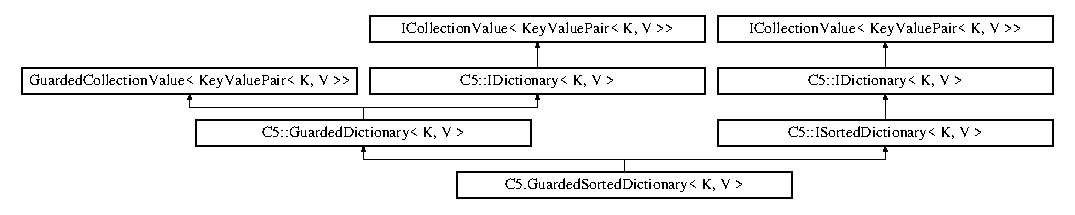
\includegraphics[height=2.448087cm]{class_c5_1_1_guarded_sorted_dictionary}
\end{center}
\end{figure}
\subsection*{Public Member Functions}
\begin{DoxyCompactItemize}
\item 
\hyperlink{class_c5_1_1_guarded_sorted_dictionary_a8087ccd945c7ead84c3dd794a78862a7}{Guarded\+Sorted\+Dictionary} (\hyperlink{interface_c5_1_1_i_sorted_dictionary}{I\+Sorted\+Dictionary}$<$ K, V $>$ sorteddict)
\begin{DoxyCompactList}\small\item\em Wrap a sorted dictionary in a read-\/only wrapper \end{DoxyCompactList}\item 
bool \hyperlink{class_c5_1_1_guarded_sorted_dictionary_a30ff56d7b975cb88ebd4581b25211d0b}{Try\+Predecessor} (K key, out \hyperlink{struct_c5_1_1_key_value_pair}{Key\+Value\+Pair}$<$ K, V $>$ res)
\begin{DoxyCompactList}\small\item\em Find the entry in the dictionary whose key is the predecessor of the specified key. \end{DoxyCompactList}\item 
bool \hyperlink{class_c5_1_1_guarded_sorted_dictionary_a40570bde5231945710618a5c4d861a09}{Try\+Successor} (K key, out \hyperlink{struct_c5_1_1_key_value_pair}{Key\+Value\+Pair}$<$ K, V $>$ res)
\begin{DoxyCompactList}\small\item\em Find the entry in the dictionary whose key is the successor of the specified key. \end{DoxyCompactList}\item 
bool \hyperlink{class_c5_1_1_guarded_sorted_dictionary_acc1c73977c59c65b03fcd78c6d21cf55}{Try\+Weak\+Predecessor} (K key, out \hyperlink{struct_c5_1_1_key_value_pair}{Key\+Value\+Pair}$<$ K, V $>$ res)
\begin{DoxyCompactList}\small\item\em Find the entry in the dictionary whose key is the weak predecessor of the specified key. \end{DoxyCompactList}\item 
bool \hyperlink{class_c5_1_1_guarded_sorted_dictionary_ad899ac9b2f1cc203bca856d2f56783f7}{Try\+Weak\+Successor} (K key, out \hyperlink{struct_c5_1_1_key_value_pair}{Key\+Value\+Pair}$<$ K, V $>$ res)
\begin{DoxyCompactList}\small\item\em Find the entry in the dictionary whose key is the weak successor of the specified key. \end{DoxyCompactList}\item 
\hyperlink{struct_c5_1_1_key_value_pair}{Key\+Value\+Pair}$<$ K, V $>$ \hyperlink{class_c5_1_1_guarded_sorted_dictionary_acf0256db1171ea679bb41ab88ababb23}{Predecessor} (K key)
\begin{DoxyCompactList}\small\item\em Get the entry in the wrapped dictionary whose key is the predecessor of a specified key. \end{DoxyCompactList}\item 
\hyperlink{struct_c5_1_1_key_value_pair}{Key\+Value\+Pair}$<$ K, V $>$ \hyperlink{class_c5_1_1_guarded_sorted_dictionary_ae112e4910e7e5f66482eb1a4445985c4}{Successor} (K key)
\begin{DoxyCompactList}\small\item\em Get the entry in the wrapped dictionary whose key is the successor of a specified key. \end{DoxyCompactList}\item 
\hyperlink{struct_c5_1_1_key_value_pair}{Key\+Value\+Pair}$<$ K, V $>$ \hyperlink{class_c5_1_1_guarded_sorted_dictionary_ad6d9c3358a0134cfb62866450a8a5e9a}{Weak\+Predecessor} (K key)
\begin{DoxyCompactList}\small\item\em Get the entry in the wrapped dictionary whose key is the weak predecessor of a specified key. \end{DoxyCompactList}\item 
\hyperlink{struct_c5_1_1_key_value_pair}{Key\+Value\+Pair}$<$ K, V $>$ \hyperlink{class_c5_1_1_guarded_sorted_dictionary_a3f90c53ece049565c81ec4679408189c}{Weak\+Successor} (K key)
\begin{DoxyCompactList}\small\item\em Get the entry in the wrapped dictionary whose key is the weak successor of a specified key. \end{DoxyCompactList}\item 
\hyperlink{struct_c5_1_1_key_value_pair}{Key\+Value\+Pair}$<$ K, V $>$ \hyperlink{class_c5_1_1_guarded_sorted_dictionary_a54ad8ab10783fb8a232cce502ef1ff60}{Find\+Min} ()
\item 
\hyperlink{struct_c5_1_1_key_value_pair}{Key\+Value\+Pair}$<$ K, V $>$ \hyperlink{class_c5_1_1_guarded_sorted_dictionary_a481cd0c7a47183de271df37fbbc6309f}{Delete\+Min} ()
\item 
\hyperlink{struct_c5_1_1_key_value_pair}{Key\+Value\+Pair}$<$ K, V $>$ \hyperlink{class_c5_1_1_guarded_sorted_dictionary_ad891d10d9fd40b6e1f4e7a855e65f3f4}{Find\+Max} ()
\item 
\hyperlink{struct_c5_1_1_key_value_pair}{Key\+Value\+Pair}$<$ K, V $>$ \hyperlink{class_c5_1_1_guarded_sorted_dictionary_a92b4a99e4067dba655cb186db659f707}{Delete\+Max} ()
\item 
bool \hyperlink{class_c5_1_1_guarded_sorted_dictionary_afd5cb3c0cd691c8e8dab675861bc3328}{Cut} (I\+Comparable$<$ K $>$ c, out \hyperlink{struct_c5_1_1_key_value_pair}{Key\+Value\+Pair}$<$ K, V $>$ low\+Entry, out bool low\+Is\+Valid, out \hyperlink{struct_c5_1_1_key_value_pair}{Key\+Value\+Pair}$<$ K, V $>$ high\+Entry, out bool high\+Is\+Valid)
\item 
\hyperlink{interface_c5_1_1_i_directed_enumerable}{I\+Directed\+Enumerable}$<$ \hyperlink{struct_c5_1_1_key_value_pair}{Key\+Value\+Pair}$<$ K, V $>$ $>$ \hyperlink{class_c5_1_1_guarded_sorted_dictionary_a68330eda6bdc72c6db469bcbf50187cf}{Range\+From} (K bot)
\item 
\hyperlink{interface_c5_1_1_i_directed_enumerable}{I\+Directed\+Enumerable}$<$ \hyperlink{struct_c5_1_1_key_value_pair}{Key\+Value\+Pair}$<$ K, V $>$ $>$ \hyperlink{class_c5_1_1_guarded_sorted_dictionary_ac83908f5c0cdb2cc9ea56e1ace8a885a}{Range\+From\+To} (K bot, K top)
\item 
\hyperlink{interface_c5_1_1_i_directed_enumerable}{I\+Directed\+Enumerable}$<$ \hyperlink{struct_c5_1_1_key_value_pair}{Key\+Value\+Pair}$<$ K, V $>$ $>$ \hyperlink{class_c5_1_1_guarded_sorted_dictionary_ac8000944dfb9e67507e05e02f6817101}{Range\+To} (K top)
\item 
\hyperlink{interface_c5_1_1_i_directed_collection_value}{I\+Directed\+Collection\+Value}$<$ \hyperlink{struct_c5_1_1_key_value_pair}{Key\+Value\+Pair}$<$ K, V $>$ $>$ \hyperlink{class_c5_1_1_guarded_sorted_dictionary_a58cb3b60cc28c3eb6e2bfbcb15d94f77}{Range\+All} ()
\item 
void \hyperlink{class_c5_1_1_guarded_sorted_dictionary_a8416822f568f078afa22b63b3d0d54f3}{Add\+Sorted} (System.\+Collections.\+Generic.\+I\+Enumerable$<$ \hyperlink{struct_c5_1_1_key_value_pair}{Key\+Value\+Pair}$<$ K, V $>$$>$ items)
\item 
void \hyperlink{class_c5_1_1_guarded_sorted_dictionary_ab248a29f9178874604ac2679273aa464}{Remove\+Range\+From} (K low)
\item 
void \hyperlink{class_c5_1_1_guarded_sorted_dictionary_a5900826397cc5997c91845695de842b5}{Remove\+Range\+From\+To} (K low, K hi)
\item 
void \hyperlink{class_c5_1_1_guarded_sorted_dictionary_a8c9d699464fa0641698dfd289bd17fd6}{Remove\+Range\+To} (K hi)
\end{DoxyCompactItemize}
\subsection*{Properties}
\begin{DoxyCompactItemize}
\item 
S\+C\+G.\+I\+Comparer$<$ K $>$ \hyperlink{class_c5_1_1_guarded_sorted_dictionary_a8ad47ad9b7269053670c95950fd8feff}{Comparer}\hspace{0.3cm}{\ttfamily  \mbox{[}get\mbox{]}}
\begin{DoxyCompactList}\small\item\em The key comparer used by this dictionary. \end{DoxyCompactList}\item 
new \hyperlink{interface_c5_1_1_i_sorted}{I\+Sorted}$<$ K $>$ \hyperlink{class_c5_1_1_guarded_sorted_dictionary_ac122f90f3bc375a5d0a6d12e15d582bb}{Keys}\hspace{0.3cm}{\ttfamily  \mbox{[}get\mbox{]}}
\end{DoxyCompactItemize}


\subsection{Detailed Description}
A read-\/only wrapper for a sorted dictionary. 

{\itshape Suitable for wrapping a Dictionary. T\+:\+C5.\+Dictionary`2} 

\subsection{Constructor \& Destructor Documentation}
\hypertarget{class_c5_1_1_guarded_sorted_dictionary_a8087ccd945c7ead84c3dd794a78862a7}{}\index{C5\+::\+Guarded\+Sorted\+Dictionary@{C5\+::\+Guarded\+Sorted\+Dictionary}!Guarded\+Sorted\+Dictionary@{Guarded\+Sorted\+Dictionary}}
\index{Guarded\+Sorted\+Dictionary@{Guarded\+Sorted\+Dictionary}!C5\+::\+Guarded\+Sorted\+Dictionary@{C5\+::\+Guarded\+Sorted\+Dictionary}}
\subsubsection[{Guarded\+Sorted\+Dictionary(\+I\+Sorted\+Dictionary$<$ K, V $>$ sorteddict)}]{\setlength{\rightskip}{0pt plus 5cm}{\bf C5.\+Guarded\+Sorted\+Dictionary}$<$ K, V $>$.{\bf Guarded\+Sorted\+Dictionary} (
\begin{DoxyParamCaption}
\item[{{\bf I\+Sorted\+Dictionary}$<$ K, V $>$}]{sorteddict}
\end{DoxyParamCaption}
)}\label{class_c5_1_1_guarded_sorted_dictionary_a8087ccd945c7ead84c3dd794a78862a7}


Wrap a sorted dictionary in a read-\/only wrapper 


\begin{DoxyParams}{Parameters}
{\em sorteddict} & the dictionary\\
\hline
\end{DoxyParams}


\subsection{Member Function Documentation}
\hypertarget{class_c5_1_1_guarded_sorted_dictionary_a8416822f568f078afa22b63b3d0d54f3}{}\index{C5\+::\+Guarded\+Sorted\+Dictionary@{C5\+::\+Guarded\+Sorted\+Dictionary}!Add\+Sorted@{Add\+Sorted}}
\index{Add\+Sorted@{Add\+Sorted}!C5\+::\+Guarded\+Sorted\+Dictionary@{C5\+::\+Guarded\+Sorted\+Dictionary}}
\subsubsection[{Add\+Sorted(\+System.\+Collections.\+Generic.\+I\+Enumerable$<$ Key\+Value\+Pair$<$ K, V $>$$>$ items)}]{\setlength{\rightskip}{0pt plus 5cm}void {\bf C5.\+Guarded\+Sorted\+Dictionary}$<$ K, V $>$.Add\+Sorted (
\begin{DoxyParamCaption}
\item[{System.\+Collections.\+Generic.\+I\+Enumerable$<$ {\bf Key\+Value\+Pair}$<$ K, V $>$$>$}]{items}
\end{DoxyParamCaption}
)}\label{class_c5_1_1_guarded_sorted_dictionary_a8416822f568f078afa22b63b3d0d54f3}





\begin{DoxyExceptions}{Exceptions}
{\em \hyperlink{class_c5_1_1_read_only_collection_exception}{Read\+Only\+Collection\+Exception}} & since this is a read-\/only wrappper\\
\hline
\end{DoxyExceptions}

\begin{DoxyParams}{Parameters}
{\em items} & \\
\hline
\end{DoxyParams}


Implements \hyperlink{interface_c5_1_1_i_sorted_dictionary_a21c08676216f78ef7f05b2139e5de3c3}{C5.\+I\+Sorted\+Dictionary$<$ K, V $>$}.

\hypertarget{class_c5_1_1_guarded_sorted_dictionary_afd5cb3c0cd691c8e8dab675861bc3328}{}\index{C5\+::\+Guarded\+Sorted\+Dictionary@{C5\+::\+Guarded\+Sorted\+Dictionary}!Cut@{Cut}}
\index{Cut@{Cut}!C5\+::\+Guarded\+Sorted\+Dictionary@{C5\+::\+Guarded\+Sorted\+Dictionary}}
\subsubsection[{Cut(\+I\+Comparable$<$ K $>$ c, out Key\+Value\+Pair$<$ K, V $>$ low\+Entry, out bool low\+Is\+Valid, out Key\+Value\+Pair$<$ K, V $>$ high\+Entry, out bool high\+Is\+Valid)}]{\setlength{\rightskip}{0pt plus 5cm}bool {\bf C5.\+Guarded\+Sorted\+Dictionary}$<$ K, V $>$.Cut (
\begin{DoxyParamCaption}
\item[{I\+Comparable$<$ K $>$}]{c, }
\item[{out {\bf Key\+Value\+Pair}$<$ K, V $>$}]{low\+Entry, }
\item[{out bool}]{low\+Is\+Valid, }
\item[{out {\bf Key\+Value\+Pair}$<$ K, V $>$}]{high\+Entry, }
\item[{out bool}]{high\+Is\+Valid}
\end{DoxyParamCaption}
)}\label{class_c5_1_1_guarded_sorted_dictionary_afd5cb3c0cd691c8e8dab675861bc3328}





\begin{DoxyParams}{Parameters}
{\em c} & \\
\hline
{\em low\+Entry} & \\
\hline
{\em low\+Is\+Valid} & \\
\hline
{\em high\+Entry} & \\
\hline
{\em high\+Is\+Valid} & \\
\hline
\end{DoxyParams}
\begin{DoxyReturn}{Returns}

\end{DoxyReturn}


Implements \hyperlink{interface_c5_1_1_i_sorted_dictionary_a28731370f84789bb4535ed92b2e38460}{C5.\+I\+Sorted\+Dictionary$<$ K, V $>$}.

\hypertarget{class_c5_1_1_guarded_sorted_dictionary_a92b4a99e4067dba655cb186db659f707}{}\index{C5\+::\+Guarded\+Sorted\+Dictionary@{C5\+::\+Guarded\+Sorted\+Dictionary}!Delete\+Max@{Delete\+Max}}
\index{Delete\+Max@{Delete\+Max}!C5\+::\+Guarded\+Sorted\+Dictionary@{C5\+::\+Guarded\+Sorted\+Dictionary}}
\subsubsection[{Delete\+Max()}]{\setlength{\rightskip}{0pt plus 5cm}{\bf Key\+Value\+Pair}$<$K, V$>$ {\bf C5.\+Guarded\+Sorted\+Dictionary}$<$ K, V $>$.Delete\+Max (
\begin{DoxyParamCaption}
{}
\end{DoxyParamCaption}
)}\label{class_c5_1_1_guarded_sorted_dictionary_a92b4a99e4067dba655cb186db659f707}





\begin{DoxyExceptions}{Exceptions}
{\em \hyperlink{class_c5_1_1_read_only_collection_exception}{Read\+Only\+Collection\+Exception}} & since this is a read-\/only wrappper\\
\hline
\end{DoxyExceptions}
\begin{DoxyReturn}{Returns}

\end{DoxyReturn}


Implements \hyperlink{interface_c5_1_1_i_sorted_dictionary_ab06a9effc3f2da79a4e446f5aa078d3b}{C5.\+I\+Sorted\+Dictionary$<$ K, V $>$}.

\hypertarget{class_c5_1_1_guarded_sorted_dictionary_a481cd0c7a47183de271df37fbbc6309f}{}\index{C5\+::\+Guarded\+Sorted\+Dictionary@{C5\+::\+Guarded\+Sorted\+Dictionary}!Delete\+Min@{Delete\+Min}}
\index{Delete\+Min@{Delete\+Min}!C5\+::\+Guarded\+Sorted\+Dictionary@{C5\+::\+Guarded\+Sorted\+Dictionary}}
\subsubsection[{Delete\+Min()}]{\setlength{\rightskip}{0pt plus 5cm}{\bf Key\+Value\+Pair}$<$K, V$>$ {\bf C5.\+Guarded\+Sorted\+Dictionary}$<$ K, V $>$.Delete\+Min (
\begin{DoxyParamCaption}
{}
\end{DoxyParamCaption}
)}\label{class_c5_1_1_guarded_sorted_dictionary_a481cd0c7a47183de271df37fbbc6309f}





\begin{DoxyExceptions}{Exceptions}
{\em \hyperlink{class_c5_1_1_read_only_collection_exception}{Read\+Only\+Collection\+Exception}} & since this is a read-\/only wrappper\\
\hline
\end{DoxyExceptions}
\begin{DoxyReturn}{Returns}

\end{DoxyReturn}


Implements \hyperlink{interface_c5_1_1_i_sorted_dictionary_a4b4c8891f922d9f2d66f4070dab9bd0a}{C5.\+I\+Sorted\+Dictionary$<$ K, V $>$}.

\hypertarget{class_c5_1_1_guarded_sorted_dictionary_ad891d10d9fd40b6e1f4e7a855e65f3f4}{}\index{C5\+::\+Guarded\+Sorted\+Dictionary@{C5\+::\+Guarded\+Sorted\+Dictionary}!Find\+Max@{Find\+Max}}
\index{Find\+Max@{Find\+Max}!C5\+::\+Guarded\+Sorted\+Dictionary@{C5\+::\+Guarded\+Sorted\+Dictionary}}
\subsubsection[{Find\+Max()}]{\setlength{\rightskip}{0pt plus 5cm}{\bf Key\+Value\+Pair}$<$K, V$>$ {\bf C5.\+Guarded\+Sorted\+Dictionary}$<$ K, V $>$.Find\+Max (
\begin{DoxyParamCaption}
{}
\end{DoxyParamCaption}
)}\label{class_c5_1_1_guarded_sorted_dictionary_ad891d10d9fd40b6e1f4e7a855e65f3f4}




\begin{DoxyReturn}{Returns}

\end{DoxyReturn}


Implements \hyperlink{interface_c5_1_1_i_sorted_dictionary_ae532ee9a31de850bac9f115509486225}{C5.\+I\+Sorted\+Dictionary$<$ K, V $>$}.

\hypertarget{class_c5_1_1_guarded_sorted_dictionary_a54ad8ab10783fb8a232cce502ef1ff60}{}\index{C5\+::\+Guarded\+Sorted\+Dictionary@{C5\+::\+Guarded\+Sorted\+Dictionary}!Find\+Min@{Find\+Min}}
\index{Find\+Min@{Find\+Min}!C5\+::\+Guarded\+Sorted\+Dictionary@{C5\+::\+Guarded\+Sorted\+Dictionary}}
\subsubsection[{Find\+Min()}]{\setlength{\rightskip}{0pt plus 5cm}{\bf Key\+Value\+Pair}$<$K, V$>$ {\bf C5.\+Guarded\+Sorted\+Dictionary}$<$ K, V $>$.Find\+Min (
\begin{DoxyParamCaption}
{}
\end{DoxyParamCaption}
)}\label{class_c5_1_1_guarded_sorted_dictionary_a54ad8ab10783fb8a232cce502ef1ff60}




\begin{DoxyReturn}{Returns}

\end{DoxyReturn}


Implements \hyperlink{interface_c5_1_1_i_sorted_dictionary_afa487d42d47f5b3730914f182880403f}{C5.\+I\+Sorted\+Dictionary$<$ K, V $>$}.

\hypertarget{class_c5_1_1_guarded_sorted_dictionary_acf0256db1171ea679bb41ab88ababb23}{}\index{C5\+::\+Guarded\+Sorted\+Dictionary@{C5\+::\+Guarded\+Sorted\+Dictionary}!Predecessor@{Predecessor}}
\index{Predecessor@{Predecessor}!C5\+::\+Guarded\+Sorted\+Dictionary@{C5\+::\+Guarded\+Sorted\+Dictionary}}
\subsubsection[{Predecessor(\+K key)}]{\setlength{\rightskip}{0pt plus 5cm}{\bf Key\+Value\+Pair}$<$K, V$>$ {\bf C5.\+Guarded\+Sorted\+Dictionary}$<$ K, V $>$.Predecessor (
\begin{DoxyParamCaption}
\item[{K}]{key}
\end{DoxyParamCaption}
)}\label{class_c5_1_1_guarded_sorted_dictionary_acf0256db1171ea679bb41ab88ababb23}


Get the entry in the wrapped dictionary whose key is the predecessor of a specified key. 


\begin{DoxyExceptions}{Exceptions}
{\em \hyperlink{class_c5_1_1_no_such_item_exception}{No\+Such\+Item\+Exception}} & if no such entry exists \\
\hline
\end{DoxyExceptions}

\begin{DoxyParams}{Parameters}
{\em key} & The key\\
\hline
\end{DoxyParams}
\begin{DoxyReturn}{Returns}
The entry
\end{DoxyReturn}


Implements \hyperlink{interface_c5_1_1_i_sorted_dictionary_ab64ecd53de02894b0d64939911fce071}{C5.\+I\+Sorted\+Dictionary$<$ K, V $>$}.

\hypertarget{class_c5_1_1_guarded_sorted_dictionary_a58cb3b60cc28c3eb6e2bfbcb15d94f77}{}\index{C5\+::\+Guarded\+Sorted\+Dictionary@{C5\+::\+Guarded\+Sorted\+Dictionary}!Range\+All@{Range\+All}}
\index{Range\+All@{Range\+All}!C5\+::\+Guarded\+Sorted\+Dictionary@{C5\+::\+Guarded\+Sorted\+Dictionary}}
\subsubsection[{Range\+All()}]{\setlength{\rightskip}{0pt plus 5cm}{\bf I\+Directed\+Collection\+Value}$<${\bf Key\+Value\+Pair}$<$K, V$>$ $>$ {\bf C5.\+Guarded\+Sorted\+Dictionary}$<$ K, V $>$.Range\+All (
\begin{DoxyParamCaption}
{}
\end{DoxyParamCaption}
)}\label{class_c5_1_1_guarded_sorted_dictionary_a58cb3b60cc28c3eb6e2bfbcb15d94f77}




\begin{DoxyReturn}{Returns}

\end{DoxyReturn}


Implements \hyperlink{interface_c5_1_1_i_sorted_dictionary_a96e38a0085b3e530c6fdb8b3ffc40848}{C5.\+I\+Sorted\+Dictionary$<$ K, V $>$}.

\hypertarget{class_c5_1_1_guarded_sorted_dictionary_a68330eda6bdc72c6db469bcbf50187cf}{}\index{C5\+::\+Guarded\+Sorted\+Dictionary@{C5\+::\+Guarded\+Sorted\+Dictionary}!Range\+From@{Range\+From}}
\index{Range\+From@{Range\+From}!C5\+::\+Guarded\+Sorted\+Dictionary@{C5\+::\+Guarded\+Sorted\+Dictionary}}
\subsubsection[{Range\+From(\+K bot)}]{\setlength{\rightskip}{0pt plus 5cm}{\bf I\+Directed\+Enumerable}$<${\bf Key\+Value\+Pair}$<$K, V$>$ $>$ {\bf C5.\+Guarded\+Sorted\+Dictionary}$<$ K, V $>$.Range\+From (
\begin{DoxyParamCaption}
\item[{K}]{bot}
\end{DoxyParamCaption}
)}\label{class_c5_1_1_guarded_sorted_dictionary_a68330eda6bdc72c6db469bcbf50187cf}





\begin{DoxyParams}{Parameters}
{\em bot} & \\
\hline
\end{DoxyParams}
\begin{DoxyReturn}{Returns}

\end{DoxyReturn}


Implements \hyperlink{interface_c5_1_1_i_sorted_dictionary_afafbf6064911808de36b781dd8085419}{C5.\+I\+Sorted\+Dictionary$<$ K, V $>$}.

\hypertarget{class_c5_1_1_guarded_sorted_dictionary_ac83908f5c0cdb2cc9ea56e1ace8a885a}{}\index{C5\+::\+Guarded\+Sorted\+Dictionary@{C5\+::\+Guarded\+Sorted\+Dictionary}!Range\+From\+To@{Range\+From\+To}}
\index{Range\+From\+To@{Range\+From\+To}!C5\+::\+Guarded\+Sorted\+Dictionary@{C5\+::\+Guarded\+Sorted\+Dictionary}}
\subsubsection[{Range\+From\+To(\+K bot, K top)}]{\setlength{\rightskip}{0pt plus 5cm}{\bf I\+Directed\+Enumerable}$<${\bf Key\+Value\+Pair}$<$K, V$>$ $>$ {\bf C5.\+Guarded\+Sorted\+Dictionary}$<$ K, V $>$.Range\+From\+To (
\begin{DoxyParamCaption}
\item[{K}]{bot, }
\item[{K}]{top}
\end{DoxyParamCaption}
)}\label{class_c5_1_1_guarded_sorted_dictionary_ac83908f5c0cdb2cc9ea56e1ace8a885a}





\begin{DoxyParams}{Parameters}
{\em bot} & \\
\hline
{\em top} & \\
\hline
\end{DoxyParams}
\begin{DoxyReturn}{Returns}

\end{DoxyReturn}


Implements \hyperlink{interface_c5_1_1_i_sorted_dictionary_a081b4c43958d18e8ee92dc234d5e8adc}{C5.\+I\+Sorted\+Dictionary$<$ K, V $>$}.

\hypertarget{class_c5_1_1_guarded_sorted_dictionary_ac8000944dfb9e67507e05e02f6817101}{}\index{C5\+::\+Guarded\+Sorted\+Dictionary@{C5\+::\+Guarded\+Sorted\+Dictionary}!Range\+To@{Range\+To}}
\index{Range\+To@{Range\+To}!C5\+::\+Guarded\+Sorted\+Dictionary@{C5\+::\+Guarded\+Sorted\+Dictionary}}
\subsubsection[{Range\+To(\+K top)}]{\setlength{\rightskip}{0pt plus 5cm}{\bf I\+Directed\+Enumerable}$<${\bf Key\+Value\+Pair}$<$K, V$>$ $>$ {\bf C5.\+Guarded\+Sorted\+Dictionary}$<$ K, V $>$.Range\+To (
\begin{DoxyParamCaption}
\item[{K}]{top}
\end{DoxyParamCaption}
)}\label{class_c5_1_1_guarded_sorted_dictionary_ac8000944dfb9e67507e05e02f6817101}





\begin{DoxyParams}{Parameters}
{\em top} & \\
\hline
\end{DoxyParams}
\begin{DoxyReturn}{Returns}

\end{DoxyReturn}


Implements \hyperlink{interface_c5_1_1_i_sorted_dictionary_aa595a13cff654c2a9b4a257402ffa5a1}{C5.\+I\+Sorted\+Dictionary$<$ K, V $>$}.

\hypertarget{class_c5_1_1_guarded_sorted_dictionary_ab248a29f9178874604ac2679273aa464}{}\index{C5\+::\+Guarded\+Sorted\+Dictionary@{C5\+::\+Guarded\+Sorted\+Dictionary}!Remove\+Range\+From@{Remove\+Range\+From}}
\index{Remove\+Range\+From@{Remove\+Range\+From}!C5\+::\+Guarded\+Sorted\+Dictionary@{C5\+::\+Guarded\+Sorted\+Dictionary}}
\subsubsection[{Remove\+Range\+From(\+K low)}]{\setlength{\rightskip}{0pt plus 5cm}void {\bf C5.\+Guarded\+Sorted\+Dictionary}$<$ K, V $>$.Remove\+Range\+From (
\begin{DoxyParamCaption}
\item[{K}]{low}
\end{DoxyParamCaption}
)}\label{class_c5_1_1_guarded_sorted_dictionary_ab248a29f9178874604ac2679273aa464}





\begin{DoxyExceptions}{Exceptions}
{\em \hyperlink{class_c5_1_1_read_only_collection_exception}{Read\+Only\+Collection\+Exception}} & since this is a read-\/only wrappper\\
\hline
\end{DoxyExceptions}

\begin{DoxyParams}{Parameters}
{\em low} & \\
\hline
\end{DoxyParams}


Implements \hyperlink{interface_c5_1_1_i_sorted_dictionary_ae25a29f876b3f9c64e86325287e8cb9c}{C5.\+I\+Sorted\+Dictionary$<$ K, V $>$}.

\hypertarget{class_c5_1_1_guarded_sorted_dictionary_a5900826397cc5997c91845695de842b5}{}\index{C5\+::\+Guarded\+Sorted\+Dictionary@{C5\+::\+Guarded\+Sorted\+Dictionary}!Remove\+Range\+From\+To@{Remove\+Range\+From\+To}}
\index{Remove\+Range\+From\+To@{Remove\+Range\+From\+To}!C5\+::\+Guarded\+Sorted\+Dictionary@{C5\+::\+Guarded\+Sorted\+Dictionary}}
\subsubsection[{Remove\+Range\+From\+To(\+K low, K hi)}]{\setlength{\rightskip}{0pt plus 5cm}void {\bf C5.\+Guarded\+Sorted\+Dictionary}$<$ K, V $>$.Remove\+Range\+From\+To (
\begin{DoxyParamCaption}
\item[{K}]{low, }
\item[{K}]{hi}
\end{DoxyParamCaption}
)}\label{class_c5_1_1_guarded_sorted_dictionary_a5900826397cc5997c91845695de842b5}





\begin{DoxyExceptions}{Exceptions}
{\em \hyperlink{class_c5_1_1_read_only_collection_exception}{Read\+Only\+Collection\+Exception}} & since this is a read-\/only wrappper\\
\hline
\end{DoxyExceptions}

\begin{DoxyParams}{Parameters}
{\em low} & \\
\hline
{\em hi} & \\
\hline
\end{DoxyParams}


Implements \hyperlink{interface_c5_1_1_i_sorted_dictionary_acc807a1a47949798348593339560c5ed}{C5.\+I\+Sorted\+Dictionary$<$ K, V $>$}.

\hypertarget{class_c5_1_1_guarded_sorted_dictionary_a8c9d699464fa0641698dfd289bd17fd6}{}\index{C5\+::\+Guarded\+Sorted\+Dictionary@{C5\+::\+Guarded\+Sorted\+Dictionary}!Remove\+Range\+To@{Remove\+Range\+To}}
\index{Remove\+Range\+To@{Remove\+Range\+To}!C5\+::\+Guarded\+Sorted\+Dictionary@{C5\+::\+Guarded\+Sorted\+Dictionary}}
\subsubsection[{Remove\+Range\+To(\+K hi)}]{\setlength{\rightskip}{0pt plus 5cm}void {\bf C5.\+Guarded\+Sorted\+Dictionary}$<$ K, V $>$.Remove\+Range\+To (
\begin{DoxyParamCaption}
\item[{K}]{hi}
\end{DoxyParamCaption}
)}\label{class_c5_1_1_guarded_sorted_dictionary_a8c9d699464fa0641698dfd289bd17fd6}





\begin{DoxyExceptions}{Exceptions}
{\em \hyperlink{class_c5_1_1_read_only_collection_exception}{Read\+Only\+Collection\+Exception}} & since this is a read-\/only wrappper\\
\hline
\end{DoxyExceptions}

\begin{DoxyParams}{Parameters}
{\em hi} & \\
\hline
\end{DoxyParams}


Implements \hyperlink{interface_c5_1_1_i_sorted_dictionary_a43cc5a30d8f6f9096311a658be0a833e}{C5.\+I\+Sorted\+Dictionary$<$ K, V $>$}.

\hypertarget{class_c5_1_1_guarded_sorted_dictionary_ae112e4910e7e5f66482eb1a4445985c4}{}\index{C5\+::\+Guarded\+Sorted\+Dictionary@{C5\+::\+Guarded\+Sorted\+Dictionary}!Successor@{Successor}}
\index{Successor@{Successor}!C5\+::\+Guarded\+Sorted\+Dictionary@{C5\+::\+Guarded\+Sorted\+Dictionary}}
\subsubsection[{Successor(\+K key)}]{\setlength{\rightskip}{0pt plus 5cm}{\bf Key\+Value\+Pair}$<$K, V$>$ {\bf C5.\+Guarded\+Sorted\+Dictionary}$<$ K, V $>$.Successor (
\begin{DoxyParamCaption}
\item[{K}]{key}
\end{DoxyParamCaption}
)}\label{class_c5_1_1_guarded_sorted_dictionary_ae112e4910e7e5f66482eb1a4445985c4}


Get the entry in the wrapped dictionary whose key is the successor of a specified key. 


\begin{DoxyExceptions}{Exceptions}
{\em \hyperlink{class_c5_1_1_no_such_item_exception}{No\+Such\+Item\+Exception}} & if no such entry exists \\
\hline
\end{DoxyExceptions}

\begin{DoxyParams}{Parameters}
{\em key} & The key\\
\hline
\end{DoxyParams}
\begin{DoxyReturn}{Returns}
The entry
\end{DoxyReturn}


Implements \hyperlink{interface_c5_1_1_i_sorted_dictionary_af8c2971bff5e52c471f19764d9d90312}{C5.\+I\+Sorted\+Dictionary$<$ K, V $>$}.

\hypertarget{class_c5_1_1_guarded_sorted_dictionary_a30ff56d7b975cb88ebd4581b25211d0b}{}\index{C5\+::\+Guarded\+Sorted\+Dictionary@{C5\+::\+Guarded\+Sorted\+Dictionary}!Try\+Predecessor@{Try\+Predecessor}}
\index{Try\+Predecessor@{Try\+Predecessor}!C5\+::\+Guarded\+Sorted\+Dictionary@{C5\+::\+Guarded\+Sorted\+Dictionary}}
\subsubsection[{Try\+Predecessor(\+K key, out Key\+Value\+Pair$<$ K, V $>$ res)}]{\setlength{\rightskip}{0pt plus 5cm}bool {\bf C5.\+Guarded\+Sorted\+Dictionary}$<$ K, V $>$.Try\+Predecessor (
\begin{DoxyParamCaption}
\item[{K}]{key, }
\item[{out {\bf Key\+Value\+Pair}$<$ K, V $>$}]{res}
\end{DoxyParamCaption}
)}\label{class_c5_1_1_guarded_sorted_dictionary_a30ff56d7b975cb88ebd4581b25211d0b}


Find the entry in the dictionary whose key is the predecessor of the specified key. 


\begin{DoxyParams}{Parameters}
{\em key} & The key\\
\hline
{\em res} & The predecessor, if any\\
\hline
\end{DoxyParams}
\begin{DoxyReturn}{Returns}
True if key has a predecessor
\end{DoxyReturn}


Implements \hyperlink{interface_c5_1_1_i_sorted_dictionary_a6af39c1f97f7fa86559edb9fd87975b8}{C5.\+I\+Sorted\+Dictionary$<$ K, V $>$}.

\hypertarget{class_c5_1_1_guarded_sorted_dictionary_a40570bde5231945710618a5c4d861a09}{}\index{C5\+::\+Guarded\+Sorted\+Dictionary@{C5\+::\+Guarded\+Sorted\+Dictionary}!Try\+Successor@{Try\+Successor}}
\index{Try\+Successor@{Try\+Successor}!C5\+::\+Guarded\+Sorted\+Dictionary@{C5\+::\+Guarded\+Sorted\+Dictionary}}
\subsubsection[{Try\+Successor(\+K key, out Key\+Value\+Pair$<$ K, V $>$ res)}]{\setlength{\rightskip}{0pt plus 5cm}bool {\bf C5.\+Guarded\+Sorted\+Dictionary}$<$ K, V $>$.Try\+Successor (
\begin{DoxyParamCaption}
\item[{K}]{key, }
\item[{out {\bf Key\+Value\+Pair}$<$ K, V $>$}]{res}
\end{DoxyParamCaption}
)}\label{class_c5_1_1_guarded_sorted_dictionary_a40570bde5231945710618a5c4d861a09}


Find the entry in the dictionary whose key is the successor of the specified key. 


\begin{DoxyParams}{Parameters}
{\em key} & The key\\
\hline
{\em res} & The successor, if any\\
\hline
\end{DoxyParams}
\begin{DoxyReturn}{Returns}
True if the key has a successor
\end{DoxyReturn}


Implements \hyperlink{interface_c5_1_1_i_sorted_dictionary_ac1448e6b319536dfb28e8b1672a5040f}{C5.\+I\+Sorted\+Dictionary$<$ K, V $>$}.

\hypertarget{class_c5_1_1_guarded_sorted_dictionary_acc1c73977c59c65b03fcd78c6d21cf55}{}\index{C5\+::\+Guarded\+Sorted\+Dictionary@{C5\+::\+Guarded\+Sorted\+Dictionary}!Try\+Weak\+Predecessor@{Try\+Weak\+Predecessor}}
\index{Try\+Weak\+Predecessor@{Try\+Weak\+Predecessor}!C5\+::\+Guarded\+Sorted\+Dictionary@{C5\+::\+Guarded\+Sorted\+Dictionary}}
\subsubsection[{Try\+Weak\+Predecessor(\+K key, out Key\+Value\+Pair$<$ K, V $>$ res)}]{\setlength{\rightskip}{0pt plus 5cm}bool {\bf C5.\+Guarded\+Sorted\+Dictionary}$<$ K, V $>$.Try\+Weak\+Predecessor (
\begin{DoxyParamCaption}
\item[{K}]{key, }
\item[{out {\bf Key\+Value\+Pair}$<$ K, V $>$}]{res}
\end{DoxyParamCaption}
)}\label{class_c5_1_1_guarded_sorted_dictionary_acc1c73977c59c65b03fcd78c6d21cf55}


Find the entry in the dictionary whose key is the weak predecessor of the specified key. 


\begin{DoxyParams}{Parameters}
{\em key} & The key\\
\hline
{\em res} & The predecessor, if any\\
\hline
\end{DoxyParams}
\begin{DoxyReturn}{Returns}
True if key has a weak predecessor
\end{DoxyReturn}


Implements \hyperlink{interface_c5_1_1_i_sorted_dictionary_a2a0e18f33ee744e70c5efd2e737a0083}{C5.\+I\+Sorted\+Dictionary$<$ K, V $>$}.

\hypertarget{class_c5_1_1_guarded_sorted_dictionary_ad899ac9b2f1cc203bca856d2f56783f7}{}\index{C5\+::\+Guarded\+Sorted\+Dictionary@{C5\+::\+Guarded\+Sorted\+Dictionary}!Try\+Weak\+Successor@{Try\+Weak\+Successor}}
\index{Try\+Weak\+Successor@{Try\+Weak\+Successor}!C5\+::\+Guarded\+Sorted\+Dictionary@{C5\+::\+Guarded\+Sorted\+Dictionary}}
\subsubsection[{Try\+Weak\+Successor(\+K key, out Key\+Value\+Pair$<$ K, V $>$ res)}]{\setlength{\rightskip}{0pt plus 5cm}bool {\bf C5.\+Guarded\+Sorted\+Dictionary}$<$ K, V $>$.Try\+Weak\+Successor (
\begin{DoxyParamCaption}
\item[{K}]{key, }
\item[{out {\bf Key\+Value\+Pair}$<$ K, V $>$}]{res}
\end{DoxyParamCaption}
)}\label{class_c5_1_1_guarded_sorted_dictionary_ad899ac9b2f1cc203bca856d2f56783f7}


Find the entry in the dictionary whose key is the weak successor of the specified key. 


\begin{DoxyParams}{Parameters}
{\em key} & The key\\
\hline
{\em res} & The weak successor, if any\\
\hline
\end{DoxyParams}
\begin{DoxyReturn}{Returns}
True if the key has a weak successor
\end{DoxyReturn}


Implements \hyperlink{interface_c5_1_1_i_sorted_dictionary_aae858ab66e83568973c0effdfda6841b}{C5.\+I\+Sorted\+Dictionary$<$ K, V $>$}.

\hypertarget{class_c5_1_1_guarded_sorted_dictionary_ad6d9c3358a0134cfb62866450a8a5e9a}{}\index{C5\+::\+Guarded\+Sorted\+Dictionary@{C5\+::\+Guarded\+Sorted\+Dictionary}!Weak\+Predecessor@{Weak\+Predecessor}}
\index{Weak\+Predecessor@{Weak\+Predecessor}!C5\+::\+Guarded\+Sorted\+Dictionary@{C5\+::\+Guarded\+Sorted\+Dictionary}}
\subsubsection[{Weak\+Predecessor(\+K key)}]{\setlength{\rightskip}{0pt plus 5cm}{\bf Key\+Value\+Pair}$<$K, V$>$ {\bf C5.\+Guarded\+Sorted\+Dictionary}$<$ K, V $>$.Weak\+Predecessor (
\begin{DoxyParamCaption}
\item[{K}]{key}
\end{DoxyParamCaption}
)}\label{class_c5_1_1_guarded_sorted_dictionary_ad6d9c3358a0134cfb62866450a8a5e9a}


Get the entry in the wrapped dictionary whose key is the weak predecessor of a specified key. 


\begin{DoxyExceptions}{Exceptions}
{\em \hyperlink{class_c5_1_1_no_such_item_exception}{No\+Such\+Item\+Exception}} & if no such entry exists \\
\hline
\end{DoxyExceptions}

\begin{DoxyParams}{Parameters}
{\em key} & The key\\
\hline
\end{DoxyParams}
\begin{DoxyReturn}{Returns}
The entry
\end{DoxyReturn}


Implements \hyperlink{interface_c5_1_1_i_sorted_dictionary_ad090cecc22bc2e5a09fe3b0ef7afd5de}{C5.\+I\+Sorted\+Dictionary$<$ K, V $>$}.

\hypertarget{class_c5_1_1_guarded_sorted_dictionary_a3f90c53ece049565c81ec4679408189c}{}\index{C5\+::\+Guarded\+Sorted\+Dictionary@{C5\+::\+Guarded\+Sorted\+Dictionary}!Weak\+Successor@{Weak\+Successor}}
\index{Weak\+Successor@{Weak\+Successor}!C5\+::\+Guarded\+Sorted\+Dictionary@{C5\+::\+Guarded\+Sorted\+Dictionary}}
\subsubsection[{Weak\+Successor(\+K key)}]{\setlength{\rightskip}{0pt plus 5cm}{\bf Key\+Value\+Pair}$<$K, V$>$ {\bf C5.\+Guarded\+Sorted\+Dictionary}$<$ K, V $>$.Weak\+Successor (
\begin{DoxyParamCaption}
\item[{K}]{key}
\end{DoxyParamCaption}
)}\label{class_c5_1_1_guarded_sorted_dictionary_a3f90c53ece049565c81ec4679408189c}


Get the entry in the wrapped dictionary whose key is the weak successor of a specified key. 


\begin{DoxyExceptions}{Exceptions}
{\em \hyperlink{class_c5_1_1_no_such_item_exception}{No\+Such\+Item\+Exception}} & if no such entry exists \\
\hline
\end{DoxyExceptions}

\begin{DoxyParams}{Parameters}
{\em key} & The key\\
\hline
\end{DoxyParams}
\begin{DoxyReturn}{Returns}
The entry
\end{DoxyReturn}


Implements \hyperlink{interface_c5_1_1_i_sorted_dictionary_a3829a2cfb58bc90c600eb2fcc12e1d25}{C5.\+I\+Sorted\+Dictionary$<$ K, V $>$}.



\subsection{Property Documentation}
\hypertarget{class_c5_1_1_guarded_sorted_dictionary_a8ad47ad9b7269053670c95950fd8feff}{}\index{C5\+::\+Guarded\+Sorted\+Dictionary@{C5\+::\+Guarded\+Sorted\+Dictionary}!Comparer@{Comparer}}
\index{Comparer@{Comparer}!C5\+::\+Guarded\+Sorted\+Dictionary@{C5\+::\+Guarded\+Sorted\+Dictionary}}
\subsubsection[{Comparer}]{\setlength{\rightskip}{0pt plus 5cm}S\+C\+G.\+I\+Comparer$<$K$>$ {\bf C5.\+Guarded\+Sorted\+Dictionary}$<$ K, V $>$.Comparer\hspace{0.3cm}{\ttfamily [get]}}\label{class_c5_1_1_guarded_sorted_dictionary_a8ad47ad9b7269053670c95950fd8feff}


The key comparer used by this dictionary. 

\hypertarget{class_c5_1_1_guarded_sorted_dictionary_ac122f90f3bc375a5d0a6d12e15d582bb}{}\index{C5\+::\+Guarded\+Sorted\+Dictionary@{C5\+::\+Guarded\+Sorted\+Dictionary}!Keys@{Keys}}
\index{Keys@{Keys}!C5\+::\+Guarded\+Sorted\+Dictionary@{C5\+::\+Guarded\+Sorted\+Dictionary}}
\subsubsection[{Keys}]{\setlength{\rightskip}{0pt plus 5cm}new {\bf I\+Sorted}$<$K$>$ {\bf C5.\+Guarded\+Sorted\+Dictionary}$<$ K, V $>$.Keys\hspace{0.3cm}{\ttfamily [get]}}\label{class_c5_1_1_guarded_sorted_dictionary_ac122f90f3bc375a5d0a6d12e15d582bb}






The documentation for this class was generated from the following file\+:\begin{DoxyCompactItemize}
\item 
C\+:/\+Users/rasmusl/\+Source/\+Repos/\+C5/\+C5/\hyperlink{_wrappers_8cs}{Wrappers.\+cs}\end{DoxyCompactItemize}

\hypertarget{class_c5_1_1_hash_bag}{}\section{C5.\+Hash\+Bag$<$ T $>$ Class Template Reference}
\label{class_c5_1_1_hash_bag}\index{C5.\+Hash\+Bag$<$ T $>$@{C5.\+Hash\+Bag$<$ T $>$}}


A bag collection based on a hash table of (item,count) pairs.  


Inheritance diagram for C5.\+Hash\+Bag$<$ T $>$\+:\begin{figure}[H]
\begin{center}
\leavevmode
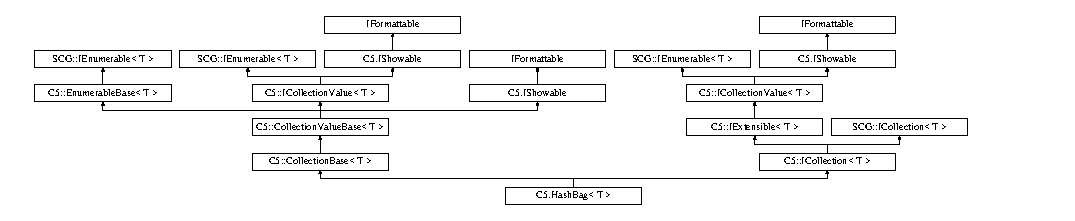
\includegraphics[height=2.526316cm]{class_c5_1_1_hash_bag}
\end{center}
\end{figure}
\subsection*{Public Member Functions}
\begin{DoxyCompactItemize}
\item 
\hyperlink{class_c5_1_1_hash_bag_a1f2efb2a869ab3cd1cc401044cfb4cdd}{Hash\+Bag} ()
\begin{DoxyCompactList}\small\item\em Create a hash bag with the deafult item equality\+Comparer. \end{DoxyCompactList}\item 
\hyperlink{class_c5_1_1_hash_bag_a2fd8c54c9f9e6117f6a8e4ae44b313a6}{Hash\+Bag} (S\+C\+G.\+I\+Equality\+Comparer$<$ T $>$ \hyperlink{class_c5_1_1_collection_base_a95e343400be0e8f3f8d6310f1aaf2cc6}{itemequality\+Comparer})
\begin{DoxyCompactList}\small\item\em Create a hash bag with an external item equality\+Comparer. \end{DoxyCompactList}\item 
\hyperlink{class_c5_1_1_hash_bag_aa2aa8a755891286b58745f230acece7d}{Hash\+Bag} (int capacity, S\+C\+G.\+I\+Equality\+Comparer$<$ T $>$ \hyperlink{class_c5_1_1_collection_base_a95e343400be0e8f3f8d6310f1aaf2cc6}{itemequality\+Comparer})
\begin{DoxyCompactList}\small\item\em Create a hash bag with external item equality\+Comparer, prescribed initial table size and default fill threshold (66\%) \end{DoxyCompactList}\item 
\hyperlink{class_c5_1_1_hash_bag_ae33cec1625f2527407e5a55946b35b6b}{Hash\+Bag} (int capacity, double fill, S\+C\+G.\+I\+Equality\+Comparer$<$ T $>$ \hyperlink{class_c5_1_1_collection_base_a95e343400be0e8f3f8d6310f1aaf2cc6}{itemequality\+Comparer})
\begin{DoxyCompactList}\small\item\em Create a hash bag with external item equality\+Comparer, prescribed initial table size and fill threshold. \end{DoxyCompactList}\item 
virtual bool \hyperlink{class_c5_1_1_hash_bag_a4ab198cd099f684fc161c4055106c2a8}{Contains} (T item)
\begin{DoxyCompactList}\small\item\em Check if an item is in the bag \end{DoxyCompactList}\item 
virtual bool \hyperlink{class_c5_1_1_hash_bag_a596f1c7fdcc7867d3b93ffb18f106655}{Find} (ref T item)
\begin{DoxyCompactList}\small\item\em Check if an item (collection equal to a given one) is in the bag and if so report the actual item object found. \end{DoxyCompactList}\item 
virtual bool \hyperlink{class_c5_1_1_hash_bag_a261d215277e57859f6a3b0dba0f31db5}{Update} (T item)
\begin{DoxyCompactList}\small\item\em Check if an item (collection equal to a given one) is in the bag and if so replace the item object in the bag with the supplied one. \end{DoxyCompactList}\item 
virtual bool \hyperlink{class_c5_1_1_hash_bag_aa464499f571def3278fb29ffd49dc9d9}{Update} (T item, out T olditem)
\item 
virtual bool \hyperlink{class_c5_1_1_hash_bag_afc84f71f4abef8b7a96f8b5d9153a270}{Find\+Or\+Add} (ref T item)
\begin{DoxyCompactList}\small\item\em Check if an item (collection equal to a given one) is in the bag. If found, report the actual item object in the bag, else add the supplied one. \end{DoxyCompactList}\item 
virtual bool \hyperlink{class_c5_1_1_hash_bag_a7d04b71113870f6bbdd936fa778d1775}{Update\+Or\+Add} (T item)
\begin{DoxyCompactList}\small\item\em Check if an item (collection equal to a supplied one) is in the bag and if so replace the item object in the set with the supplied one; else add the supplied one. \end{DoxyCompactList}\item 
virtual bool \hyperlink{class_c5_1_1_hash_bag_a22061ab9c804125e28d56a4d32aa6ee7}{Update\+Or\+Add} (T item, out T olditem)
\item 
virtual bool \hyperlink{class_c5_1_1_hash_bag_aecff446396494ee3d10ee53f5bc78ce5}{Remove} (T item)
\begin{DoxyCompactList}\small\item\em Remove one copy af an item from the bag \end{DoxyCompactList}\item 
virtual bool \hyperlink{class_c5_1_1_hash_bag_a15514e59b510fc1e5d1d4b5bc3ca16c8}{Remove} (T item, out T removeditem)
\begin{DoxyCompactList}\small\item\em Remove one copy of an item from the bag, reporting the actual matching item object. \end{DoxyCompactList}\item 
virtual void \hyperlink{class_c5_1_1_hash_bag_ab207da94ab560f22eabefaa17fdbd6d7}{Remove\+All} (S\+C\+G.\+I\+Enumerable$<$ T $>$ items)
\begin{DoxyCompactList}\small\item\em Remove all items in a supplied collection from this bag, counting multiplicities. \end{DoxyCompactList}\item 
virtual void \hyperlink{class_c5_1_1_hash_bag_a56b6eaa83ad0f3851cb48322f536f3d8}{Clear} ()
\begin{DoxyCompactList}\small\item\em Remove all items from the bag, resetting internal table to initial size. \end{DoxyCompactList}\item 
virtual void \hyperlink{class_c5_1_1_hash_bag_aa83a436a144bb83ea23059d2b9d54a45}{Retain\+All} (S\+C\+G.\+I\+Enumerable$<$ T $>$ items)
\begin{DoxyCompactList}\small\item\em Remove all items {\itshape not} in a supplied collection from this bag, counting multiplicities. \end{DoxyCompactList}\item 
virtual bool \hyperlink{class_c5_1_1_hash_bag_aff78f22f0c5e6b5dc2c550cd0d5a24e3}{Contains\+All} (S\+C\+G.\+I\+Enumerable$<$ T $>$ items)
\begin{DoxyCompactList}\small\item\em Check if all items in a supplied collection is in this bag (counting multiplicities). \end{DoxyCompactList}\item 
override T\mbox{[}$\,$\mbox{]} \hyperlink{class_c5_1_1_hash_bag_a7be4bcb7a5ef7f9414a33cfb9439e15e}{To\+Array} ()
\begin{DoxyCompactList}\small\item\em Create an array containing all items in this bag (in enumeration order). \end{DoxyCompactList}\item 
virtual int \hyperlink{class_c5_1_1_hash_bag_ae9d24cf11e28837e35dfcf9a89858a90}{Contains\+Count} (T item)
\begin{DoxyCompactList}\small\item\em Count the number of times an item is in this set. \end{DoxyCompactList}\item 
virtual \hyperlink{interface_c5_1_1_i_collection_value}{I\+Collection\+Value}$<$ T $>$ \hyperlink{class_c5_1_1_hash_bag_ab6b0278effda160df10814d87e885385}{Unique\+Items} ()
\item 
virtual \hyperlink{interface_c5_1_1_i_collection_value}{I\+Collection\+Value}$<$ \hyperlink{struct_c5_1_1_key_value_pair}{Key\+Value\+Pair}$<$ T, int $>$ $>$ \hyperlink{class_c5_1_1_hash_bag_a25efbcb614ab06216f52a7f34f74f8fc}{Item\+Multiplicities} ()
\item 
virtual void \hyperlink{class_c5_1_1_hash_bag_ac7e182e2105701436c1288feaeeef627}{Remove\+All\+Copies} (T item)
\begin{DoxyCompactList}\small\item\em Remove all copies of item from this set. \end{DoxyCompactList}\item 
override void \hyperlink{class_c5_1_1_hash_bag_ad7ffdb5c882c290aa8b398d499a9d2ac}{Copy\+To} (T\mbox{[}$\,$\mbox{]} array, int index)
\begin{DoxyCompactList}\small\item\em Copy the items of this bag to part of an array. 
\begin{DoxyExceptions}{Exceptions}
{\em Argument\+Out\+Of\+Range\+Exception} & if i is negative. 
\begin{DoxyExceptions}{Exceptions}
{\em Argument\+Exception} & if the array does not have room for the items. \\
\hline
\end{DoxyExceptions}
\\
\hline
\end{DoxyExceptions}
\end{DoxyCompactList}\item 
virtual bool \hyperlink{class_c5_1_1_hash_bag_a4cc47989ae0d25e5574558f973b85a8d}{Add} (T item)
\begin{DoxyCompactList}\small\item\em Add an item to this bag. \end{DoxyCompactList}\item 
virtual void \hyperlink{class_c5_1_1_hash_bag_a87617053c1b6c067efc395b1743e8ed0}{Add\+All} (S\+C\+G.\+I\+Enumerable$<$ T $>$ items)
\begin{DoxyCompactList}\small\item\em Add the elements from another collection with a more specialized item type to this collection. \end{DoxyCompactList}\item 
override T \hyperlink{class_c5_1_1_hash_bag_ac17786a0542bbe968fc662d5e2749265}{Choose} ()
\begin{DoxyCompactList}\small\item\em Choose some item of this collection. \end{DoxyCompactList}\item 
override S\+C\+G.\+I\+Enumerator$<$ T $>$ \hyperlink{class_c5_1_1_hash_bag_a621d77b2f8a7c3a826aace4be1d809b2}{Get\+Enumerator} ()
\begin{DoxyCompactList}\small\item\em Create an enumerator for this bag. \end{DoxyCompactList}\item 
virtual bool \hyperlink{class_c5_1_1_hash_bag_a19a4c4b0767d7ef9e015bf8b9eadd1e9}{Check} ()
\begin{DoxyCompactList}\small\item\em Test internal structure of data (invariants) \end{DoxyCompactList}\end{DoxyCompactItemize}
\subsection*{Properties}
\begin{DoxyCompactItemize}
\item 
override \hyperlink{namespace_c5_a9143bfd561fffa025d21561674758008}{Event\+Type\+Enum} \hyperlink{class_c5_1_1_hash_bag_a676d1112960f86055de24540992f6310}{Listenable\+Events}\hspace{0.3cm}{\ttfamily  \mbox{[}get\mbox{]}}
\item 
virtual \hyperlink{namespace_c5_a615ba88dcdaa8d5a3c5f833a73d7fad6}{Speed} \hyperlink{class_c5_1_1_hash_bag_aa3fed46c7ca11098f330ad791da98c31}{Contains\+Speed}\hspace{0.3cm}{\ttfamily  \mbox{[}get\mbox{]}}
\begin{DoxyCompactList}\small\item\em The complexity of the Contains operation \end{DoxyCompactList}\item 
virtual bool \hyperlink{class_c5_1_1_hash_bag_a1aee5b97f3bf34a9c75838848aeff1fa}{Allows\+Duplicates}\hspace{0.3cm}{\ttfamily  \mbox{[}get\mbox{]}}
\begin{DoxyCompactList}\small\item\em Report if this is a set collection. \end{DoxyCompactList}\item 
virtual bool \hyperlink{class_c5_1_1_hash_bag_a868b4e2fa4bdf260e0cd22663b313267}{Duplicates\+By\+Counting}\hspace{0.3cm}{\ttfamily  \mbox{[}get\mbox{]}}
\begin{DoxyCompactList}\small\item\em By convention this is true for any collection with set semantics. \end{DoxyCompactList}\end{DoxyCompactItemize}
\subsection*{Additional Inherited Members}


\subsection{Detailed Description}
A bag collection based on a hash table of (item,count) pairs. 



\subsection{Constructor \& Destructor Documentation}
\hypertarget{class_c5_1_1_hash_bag_a1f2efb2a869ab3cd1cc401044cfb4cdd}{}\index{C5\+::\+Hash\+Bag@{C5\+::\+Hash\+Bag}!Hash\+Bag@{Hash\+Bag}}
\index{Hash\+Bag@{Hash\+Bag}!C5\+::\+Hash\+Bag@{C5\+::\+Hash\+Bag}}
\subsubsection[{Hash\+Bag()}]{\setlength{\rightskip}{0pt plus 5cm}{\bf C5.\+Hash\+Bag}$<$ T $>$.{\bf Hash\+Bag} (
\begin{DoxyParamCaption}
{}
\end{DoxyParamCaption}
)}\label{class_c5_1_1_hash_bag_a1f2efb2a869ab3cd1cc401044cfb4cdd}


Create a hash bag with the deafult item equality\+Comparer. 

\hypertarget{class_c5_1_1_hash_bag_a2fd8c54c9f9e6117f6a8e4ae44b313a6}{}\index{C5\+::\+Hash\+Bag@{C5\+::\+Hash\+Bag}!Hash\+Bag@{Hash\+Bag}}
\index{Hash\+Bag@{Hash\+Bag}!C5\+::\+Hash\+Bag@{C5\+::\+Hash\+Bag}}
\subsubsection[{Hash\+Bag(\+S\+C\+G.\+I\+Equality\+Comparer$<$ T $>$ itemequality\+Comparer)}]{\setlength{\rightskip}{0pt plus 5cm}{\bf C5.\+Hash\+Bag}$<$ T $>$.{\bf Hash\+Bag} (
\begin{DoxyParamCaption}
\item[{S\+C\+G.\+I\+Equality\+Comparer$<$ T $>$}]{itemequality\+Comparer}
\end{DoxyParamCaption}
)}\label{class_c5_1_1_hash_bag_a2fd8c54c9f9e6117f6a8e4ae44b313a6}


Create a hash bag with an external item equality\+Comparer. 


\begin{DoxyParams}{Parameters}
{\em itemequality\+Comparer} & The external item equality\+Comparer.\\
\hline
\end{DoxyParams}
\hypertarget{class_c5_1_1_hash_bag_aa2aa8a755891286b58745f230acece7d}{}\index{C5\+::\+Hash\+Bag@{C5\+::\+Hash\+Bag}!Hash\+Bag@{Hash\+Bag}}
\index{Hash\+Bag@{Hash\+Bag}!C5\+::\+Hash\+Bag@{C5\+::\+Hash\+Bag}}
\subsubsection[{Hash\+Bag(int capacity, S\+C\+G.\+I\+Equality\+Comparer$<$ T $>$ itemequality\+Comparer)}]{\setlength{\rightskip}{0pt plus 5cm}{\bf C5.\+Hash\+Bag}$<$ T $>$.{\bf Hash\+Bag} (
\begin{DoxyParamCaption}
\item[{int}]{capacity, }
\item[{S\+C\+G.\+I\+Equality\+Comparer$<$ T $>$}]{itemequality\+Comparer}
\end{DoxyParamCaption}
)}\label{class_c5_1_1_hash_bag_aa2aa8a755891286b58745f230acece7d}


Create a hash bag with external item equality\+Comparer, prescribed initial table size and default fill threshold (66\%) 


\begin{DoxyParams}{Parameters}
{\em capacity} & Initial table size (rounded to power of 2, at least 16)\\
\hline
{\em itemequality\+Comparer} & The external item equality\+S\+C\+G.\+Comparer\\
\hline
\end{DoxyParams}
\hypertarget{class_c5_1_1_hash_bag_ae33cec1625f2527407e5a55946b35b6b}{}\index{C5\+::\+Hash\+Bag@{C5\+::\+Hash\+Bag}!Hash\+Bag@{Hash\+Bag}}
\index{Hash\+Bag@{Hash\+Bag}!C5\+::\+Hash\+Bag@{C5\+::\+Hash\+Bag}}
\subsubsection[{Hash\+Bag(int capacity, double fill, S\+C\+G.\+I\+Equality\+Comparer$<$ T $>$ itemequality\+Comparer)}]{\setlength{\rightskip}{0pt plus 5cm}{\bf C5.\+Hash\+Bag}$<$ T $>$.{\bf Hash\+Bag} (
\begin{DoxyParamCaption}
\item[{int}]{capacity, }
\item[{double}]{fill, }
\item[{S\+C\+G.\+I\+Equality\+Comparer$<$ T $>$}]{itemequality\+Comparer}
\end{DoxyParamCaption}
)}\label{class_c5_1_1_hash_bag_ae33cec1625f2527407e5a55946b35b6b}


Create a hash bag with external item equality\+Comparer, prescribed initial table size and fill threshold. 


\begin{DoxyParams}{Parameters}
{\em capacity} & Initial table size (rounded to power of 2, at least 16)\\
\hline
{\em fill} & Fill threshold (valid range 10\% to 90\%)\\
\hline
{\em itemequality\+Comparer} & The external item equality\+S\+C\+G.\+Comparer\\
\hline
\end{DoxyParams}


\subsection{Member Function Documentation}
\hypertarget{class_c5_1_1_hash_bag_a4cc47989ae0d25e5574558f973b85a8d}{}\index{C5\+::\+Hash\+Bag@{C5\+::\+Hash\+Bag}!Add@{Add}}
\index{Add@{Add}!C5\+::\+Hash\+Bag@{C5\+::\+Hash\+Bag}}
\subsubsection[{Add(\+T item)}]{\setlength{\rightskip}{0pt plus 5cm}virtual bool {\bf C5.\+Hash\+Bag}$<$ T $>$.Add (
\begin{DoxyParamCaption}
\item[{T}]{item}
\end{DoxyParamCaption}
)\hspace{0.3cm}{\ttfamily [virtual]}}\label{class_c5_1_1_hash_bag_a4cc47989ae0d25e5574558f973b85a8d}


Add an item to this bag. 


\begin{DoxyParams}{Parameters}
{\em item} & The item to add.\\
\hline
\end{DoxyParams}
\begin{DoxyReturn}{Returns}
Always true
\end{DoxyReturn}


Implements \hyperlink{interface_c5_1_1_i_collection_a525115f252ddca586fcbf1a0127be614}{C5.\+I\+Collection$<$ T $>$}.

\hypertarget{class_c5_1_1_hash_bag_a87617053c1b6c067efc395b1743e8ed0}{}\index{C5\+::\+Hash\+Bag@{C5\+::\+Hash\+Bag}!Add\+All@{Add\+All}}
\index{Add\+All@{Add\+All}!C5\+::\+Hash\+Bag@{C5\+::\+Hash\+Bag}}
\subsubsection[{Add\+All(\+S\+C\+G.\+I\+Enumerable$<$ T $>$ items)}]{\setlength{\rightskip}{0pt plus 5cm}virtual void {\bf C5.\+Hash\+Bag}$<$ T $>$.Add\+All (
\begin{DoxyParamCaption}
\item[{S\+C\+G.\+I\+Enumerable$<$ T $>$}]{items}
\end{DoxyParamCaption}
)\hspace{0.3cm}{\ttfamily [virtual]}}\label{class_c5_1_1_hash_bag_a87617053c1b6c067efc395b1743e8ed0}


Add the elements from another collection with a more specialized item type to this collection. 


\begin{DoxyParams}{Parameters}
{\em items} & The items to add\\
\hline
\end{DoxyParams}


Implements \hyperlink{interface_c5_1_1_i_extensible_a1fb4d50c5b340e60303da72e9d0ede6e}{C5.\+I\+Extensible$<$ T $>$}.

\hypertarget{class_c5_1_1_hash_bag_a19a4c4b0767d7ef9e015bf8b9eadd1e9}{}\index{C5\+::\+Hash\+Bag@{C5\+::\+Hash\+Bag}!Check@{Check}}
\index{Check@{Check}!C5\+::\+Hash\+Bag@{C5\+::\+Hash\+Bag}}
\subsubsection[{Check()}]{\setlength{\rightskip}{0pt plus 5cm}virtual bool {\bf C5.\+Hash\+Bag}$<$ T $>$.Check (
\begin{DoxyParamCaption}
{}
\end{DoxyParamCaption}
)\hspace{0.3cm}{\ttfamily [virtual]}}\label{class_c5_1_1_hash_bag_a19a4c4b0767d7ef9e015bf8b9eadd1e9}


Test internal structure of data (invariants) 

\begin{DoxyReturn}{Returns}
True if pass
\end{DoxyReturn}


Implements \hyperlink{interface_c5_1_1_i_extensible_aeeb6b87af61e455df42d68834d711bcb}{C5.\+I\+Extensible$<$ T $>$}.

\hypertarget{class_c5_1_1_hash_bag_ac17786a0542bbe968fc662d5e2749265}{}\index{C5\+::\+Hash\+Bag@{C5\+::\+Hash\+Bag}!Choose@{Choose}}
\index{Choose@{Choose}!C5\+::\+Hash\+Bag@{C5\+::\+Hash\+Bag}}
\subsubsection[{Choose()}]{\setlength{\rightskip}{0pt plus 5cm}override T {\bf C5.\+Hash\+Bag}$<$ T $>$.Choose (
\begin{DoxyParamCaption}
{}
\end{DoxyParamCaption}
)\hspace{0.3cm}{\ttfamily [virtual]}}\label{class_c5_1_1_hash_bag_ac17786a0542bbe968fc662d5e2749265}


Choose some item of this collection. 


\begin{DoxyExceptions}{Exceptions}
{\em \hyperlink{class_c5_1_1_no_such_item_exception}{No\+Such\+Item\+Exception}} & if collection is empty.\\
\hline
\end{DoxyExceptions}
\begin{DoxyReturn}{Returns}

\end{DoxyReturn}


Implements \hyperlink{class_c5_1_1_collection_value_base_ad7b8bd01dfd7ea8480a972f02a81608b}{C5.\+Collection\+Value\+Base$<$ T $>$}.

\hypertarget{class_c5_1_1_hash_bag_a56b6eaa83ad0f3851cb48322f536f3d8}{}\index{C5\+::\+Hash\+Bag@{C5\+::\+Hash\+Bag}!Clear@{Clear}}
\index{Clear@{Clear}!C5\+::\+Hash\+Bag@{C5\+::\+Hash\+Bag}}
\subsubsection[{Clear()}]{\setlength{\rightskip}{0pt plus 5cm}virtual void {\bf C5.\+Hash\+Bag}$<$ T $>$.Clear (
\begin{DoxyParamCaption}
{}
\end{DoxyParamCaption}
)\hspace{0.3cm}{\ttfamily [virtual]}}\label{class_c5_1_1_hash_bag_a56b6eaa83ad0f3851cb48322f536f3d8}


Remove all items from the bag, resetting internal table to initial size. 



Implements \hyperlink{interface_c5_1_1_i_collection_abd83166ac00b3d36225d988fd4603e97}{C5.\+I\+Collection$<$ T $>$}.

\hypertarget{class_c5_1_1_hash_bag_a4ab198cd099f684fc161c4055106c2a8}{}\index{C5\+::\+Hash\+Bag@{C5\+::\+Hash\+Bag}!Contains@{Contains}}
\index{Contains@{Contains}!C5\+::\+Hash\+Bag@{C5\+::\+Hash\+Bag}}
\subsubsection[{Contains(\+T item)}]{\setlength{\rightskip}{0pt plus 5cm}virtual bool {\bf C5.\+Hash\+Bag}$<$ T $>$.Contains (
\begin{DoxyParamCaption}
\item[{T}]{item}
\end{DoxyParamCaption}
)\hspace{0.3cm}{\ttfamily [virtual]}}\label{class_c5_1_1_hash_bag_a4ab198cd099f684fc161c4055106c2a8}


Check if an item is in the bag 


\begin{DoxyParams}{Parameters}
{\em item} & The item to look for\\
\hline
\end{DoxyParams}
\begin{DoxyReturn}{Returns}
True if bag contains item
\end{DoxyReturn}


Implements \hyperlink{interface_c5_1_1_i_collection_a4de01b6d77ea5eaffccc8267b4454cdd}{C5.\+I\+Collection$<$ T $>$}.

\hypertarget{class_c5_1_1_hash_bag_aff78f22f0c5e6b5dc2c550cd0d5a24e3}{}\index{C5\+::\+Hash\+Bag@{C5\+::\+Hash\+Bag}!Contains\+All@{Contains\+All}}
\index{Contains\+All@{Contains\+All}!C5\+::\+Hash\+Bag@{C5\+::\+Hash\+Bag}}
\subsubsection[{Contains\+All(\+S\+C\+G.\+I\+Enumerable$<$ T $>$ items)}]{\setlength{\rightskip}{0pt plus 5cm}virtual bool {\bf C5.\+Hash\+Bag}$<$ T $>$.Contains\+All (
\begin{DoxyParamCaption}
\item[{S\+C\+G.\+I\+Enumerable$<$ T $>$}]{items}
\end{DoxyParamCaption}
)\hspace{0.3cm}{\ttfamily [virtual]}}\label{class_c5_1_1_hash_bag_aff78f22f0c5e6b5dc2c550cd0d5a24e3}


Check if all items in a supplied collection is in this bag (counting multiplicities). 


\begin{DoxyParams}{Parameters}
{\em items} & The items to look for.\\
\hline
\end{DoxyParams}
\begin{DoxyReturn}{Returns}
True if all items are found.
\end{DoxyReturn}


Implements \hyperlink{interface_c5_1_1_i_collection_a93abf02183a46f56af8d90f1d69982a8}{C5.\+I\+Collection$<$ T $>$}.

\hypertarget{class_c5_1_1_hash_bag_ae9d24cf11e28837e35dfcf9a89858a90}{}\index{C5\+::\+Hash\+Bag@{C5\+::\+Hash\+Bag}!Contains\+Count@{Contains\+Count}}
\index{Contains\+Count@{Contains\+Count}!C5\+::\+Hash\+Bag@{C5\+::\+Hash\+Bag}}
\subsubsection[{Contains\+Count(\+T item)}]{\setlength{\rightskip}{0pt plus 5cm}virtual int {\bf C5.\+Hash\+Bag}$<$ T $>$.Contains\+Count (
\begin{DoxyParamCaption}
\item[{T}]{item}
\end{DoxyParamCaption}
)\hspace{0.3cm}{\ttfamily [virtual]}}\label{class_c5_1_1_hash_bag_ae9d24cf11e28837e35dfcf9a89858a90}


Count the number of times an item is in this set. 


\begin{DoxyParams}{Parameters}
{\em item} & The item to look for.\\
\hline
\end{DoxyParams}
\begin{DoxyReturn}{Returns}
The count
\end{DoxyReturn}


Implements \hyperlink{interface_c5_1_1_i_collection_acfe7e2c9b14c384762269edbb57b7fbe}{C5.\+I\+Collection$<$ T $>$}.

\hypertarget{class_c5_1_1_hash_bag_ad7ffdb5c882c290aa8b398d499a9d2ac}{}\index{C5\+::\+Hash\+Bag@{C5\+::\+Hash\+Bag}!Copy\+To@{Copy\+To}}
\index{Copy\+To@{Copy\+To}!C5\+::\+Hash\+Bag@{C5\+::\+Hash\+Bag}}
\subsubsection[{Copy\+To(\+T[] array, int index)}]{\setlength{\rightskip}{0pt plus 5cm}override void {\bf C5.\+Hash\+Bag}$<$ T $>$.Copy\+To (
\begin{DoxyParamCaption}
\item[{T\mbox{[}$\,$\mbox{]}}]{array, }
\item[{int}]{index}
\end{DoxyParamCaption}
)}\label{class_c5_1_1_hash_bag_ad7ffdb5c882c290aa8b398d499a9d2ac}


Copy the items of this bag to part of an array. 
\begin{DoxyExceptions}{Exceptions}
{\em Argument\+Out\+Of\+Range\+Exception} & if i is negative. 
\begin{DoxyExceptions}{Exceptions}
{\em Argument\+Exception} & if the array does not have room for the items. \\
\hline
\end{DoxyExceptions}
\\
\hline
\end{DoxyExceptions}



\begin{DoxyParams}{Parameters}
{\em array} & The array to copy to\\
\hline
{\em index} & The starting index.\\
\hline
\end{DoxyParams}


Implements \hyperlink{interface_c5_1_1_i_collection_aa2f928b7057eb84a1572307123e8239e}{C5.\+I\+Collection$<$ T $>$}.

\hypertarget{class_c5_1_1_hash_bag_a596f1c7fdcc7867d3b93ffb18f106655}{}\index{C5\+::\+Hash\+Bag@{C5\+::\+Hash\+Bag}!Find@{Find}}
\index{Find@{Find}!C5\+::\+Hash\+Bag@{C5\+::\+Hash\+Bag}}
\subsubsection[{Find(ref T item)}]{\setlength{\rightskip}{0pt plus 5cm}virtual bool {\bf C5.\+Hash\+Bag}$<$ T $>$.Find (
\begin{DoxyParamCaption}
\item[{ref T}]{item}
\end{DoxyParamCaption}
)\hspace{0.3cm}{\ttfamily [virtual]}}\label{class_c5_1_1_hash_bag_a596f1c7fdcc7867d3b93ffb18f106655}


Check if an item (collection equal to a given one) is in the bag and if so report the actual item object found. 


\begin{DoxyParams}{Parameters}
{\em item} & On entry, the item to look for. On exit the item found, if any\\
\hline
\end{DoxyParams}
\begin{DoxyReturn}{Returns}
True if bag contains item
\end{DoxyReturn}


Implements \hyperlink{interface_c5_1_1_i_collection_a96fd6cfd3df62e67922f9335b0fbbdcb}{C5.\+I\+Collection$<$ T $>$}.

\hypertarget{class_c5_1_1_hash_bag_afc84f71f4abef8b7a96f8b5d9153a270}{}\index{C5\+::\+Hash\+Bag@{C5\+::\+Hash\+Bag}!Find\+Or\+Add@{Find\+Or\+Add}}
\index{Find\+Or\+Add@{Find\+Or\+Add}!C5\+::\+Hash\+Bag@{C5\+::\+Hash\+Bag}}
\subsubsection[{Find\+Or\+Add(ref T item)}]{\setlength{\rightskip}{0pt plus 5cm}virtual bool {\bf C5.\+Hash\+Bag}$<$ T $>$.Find\+Or\+Add (
\begin{DoxyParamCaption}
\item[{ref T}]{item}
\end{DoxyParamCaption}
)\hspace{0.3cm}{\ttfamily [virtual]}}\label{class_c5_1_1_hash_bag_afc84f71f4abef8b7a96f8b5d9153a270}


Check if an item (collection equal to a given one) is in the bag. If found, report the actual item object in the bag, else add the supplied one. 


\begin{DoxyParams}{Parameters}
{\em item} & On entry, the item to look for or add. On exit the actual object found, if any.\\
\hline
\end{DoxyParams}
\begin{DoxyReturn}{Returns}
True if item was found
\end{DoxyReturn}


Implements \hyperlink{interface_c5_1_1_i_collection_a7f9e609ee1a7607596bb65aa5bdff303}{C5.\+I\+Collection$<$ T $>$}.

\hypertarget{class_c5_1_1_hash_bag_a621d77b2f8a7c3a826aace4be1d809b2}{}\index{C5\+::\+Hash\+Bag@{C5\+::\+Hash\+Bag}!Get\+Enumerator@{Get\+Enumerator}}
\index{Get\+Enumerator@{Get\+Enumerator}!C5\+::\+Hash\+Bag@{C5\+::\+Hash\+Bag}}
\subsubsection[{Get\+Enumerator()}]{\setlength{\rightskip}{0pt plus 5cm}override S\+C\+G.\+I\+Enumerator$<$T$>$ {\bf C5.\+Hash\+Bag}$<$ T $>$.Get\+Enumerator (
\begin{DoxyParamCaption}
{}
\end{DoxyParamCaption}
)\hspace{0.3cm}{\ttfamily [virtual]}}\label{class_c5_1_1_hash_bag_a621d77b2f8a7c3a826aace4be1d809b2}


Create an enumerator for this bag. 

\begin{DoxyReturn}{Returns}
The enumerator
\end{DoxyReturn}


Implements \hyperlink{class_c5_1_1_collection_base_a3b4b98e2606afecb948019412c4c2533}{C5.\+Collection\+Base$<$ T $>$}.

\hypertarget{class_c5_1_1_hash_bag_a25efbcb614ab06216f52a7f34f74f8fc}{}\index{C5\+::\+Hash\+Bag@{C5\+::\+Hash\+Bag}!Item\+Multiplicities@{Item\+Multiplicities}}
\index{Item\+Multiplicities@{Item\+Multiplicities}!C5\+::\+Hash\+Bag@{C5\+::\+Hash\+Bag}}
\subsubsection[{Item\+Multiplicities()}]{\setlength{\rightskip}{0pt plus 5cm}virtual {\bf I\+Collection\+Value}$<${\bf Key\+Value\+Pair}$<$T, int$>$ $>$ {\bf C5.\+Hash\+Bag}$<$ T $>$.Item\+Multiplicities (
\begin{DoxyParamCaption}
{}
\end{DoxyParamCaption}
)\hspace{0.3cm}{\ttfamily [virtual]}}\label{class_c5_1_1_hash_bag_a25efbcb614ab06216f52a7f34f74f8fc}




\begin{DoxyReturn}{Returns}

\end{DoxyReturn}


Implements \hyperlink{interface_c5_1_1_i_collection_a623bd834b37b299c5f4948fdb6915fef}{C5.\+I\+Collection$<$ T $>$}.

\hypertarget{class_c5_1_1_hash_bag_aecff446396494ee3d10ee53f5bc78ce5}{}\index{C5\+::\+Hash\+Bag@{C5\+::\+Hash\+Bag}!Remove@{Remove}}
\index{Remove@{Remove}!C5\+::\+Hash\+Bag@{C5\+::\+Hash\+Bag}}
\subsubsection[{Remove(\+T item)}]{\setlength{\rightskip}{0pt plus 5cm}virtual bool {\bf C5.\+Hash\+Bag}$<$ T $>$.Remove (
\begin{DoxyParamCaption}
\item[{T}]{item}
\end{DoxyParamCaption}
)\hspace{0.3cm}{\ttfamily [virtual]}}\label{class_c5_1_1_hash_bag_aecff446396494ee3d10ee53f5bc78ce5}


Remove one copy af an item from the bag 


\begin{DoxyParams}{Parameters}
{\em item} & The item to remove\\
\hline
\end{DoxyParams}
\begin{DoxyReturn}{Returns}
True if item was (found and) removed 
\end{DoxyReturn}


Implements \hyperlink{interface_c5_1_1_i_collection_ab4d6092ac09245ce46db91595fc1cdfe}{C5.\+I\+Collection$<$ T $>$}.

\hypertarget{class_c5_1_1_hash_bag_a15514e59b510fc1e5d1d4b5bc3ca16c8}{}\index{C5\+::\+Hash\+Bag@{C5\+::\+Hash\+Bag}!Remove@{Remove}}
\index{Remove@{Remove}!C5\+::\+Hash\+Bag@{C5\+::\+Hash\+Bag}}
\subsubsection[{Remove(\+T item, out T removeditem)}]{\setlength{\rightskip}{0pt plus 5cm}virtual bool {\bf C5.\+Hash\+Bag}$<$ T $>$.Remove (
\begin{DoxyParamCaption}
\item[{T}]{item, }
\item[{out T}]{removeditem}
\end{DoxyParamCaption}
)\hspace{0.3cm}{\ttfamily [virtual]}}\label{class_c5_1_1_hash_bag_a15514e59b510fc1e5d1d4b5bc3ca16c8}


Remove one copy of an item from the bag, reporting the actual matching item object. 


\begin{DoxyParams}{Parameters}
{\em item} & The value to remove.\\
\hline
{\em removeditem} & The removed value.\\
\hline
\end{DoxyParams}
\begin{DoxyReturn}{Returns}
True if item was found.
\end{DoxyReturn}


Implements \hyperlink{interface_c5_1_1_i_collection_acbd124236c3f0958a8784d9c7c2dfd16}{C5.\+I\+Collection$<$ T $>$}.

\hypertarget{class_c5_1_1_hash_bag_ab207da94ab560f22eabefaa17fdbd6d7}{}\index{C5\+::\+Hash\+Bag@{C5\+::\+Hash\+Bag}!Remove\+All@{Remove\+All}}
\index{Remove\+All@{Remove\+All}!C5\+::\+Hash\+Bag@{C5\+::\+Hash\+Bag}}
\subsubsection[{Remove\+All(\+S\+C\+G.\+I\+Enumerable$<$ T $>$ items)}]{\setlength{\rightskip}{0pt plus 5cm}virtual void {\bf C5.\+Hash\+Bag}$<$ T $>$.Remove\+All (
\begin{DoxyParamCaption}
\item[{S\+C\+G.\+I\+Enumerable$<$ T $>$}]{items}
\end{DoxyParamCaption}
)\hspace{0.3cm}{\ttfamily [virtual]}}\label{class_c5_1_1_hash_bag_ab207da94ab560f22eabefaa17fdbd6d7}


Remove all items in a supplied collection from this bag, counting multiplicities. 


\begin{DoxyParams}{Parameters}
{\em items} & The items to remove.\\
\hline
\end{DoxyParams}


Implements \hyperlink{interface_c5_1_1_i_collection_a9fb05163a1bd4b71bfd05101ff20c987}{C5.\+I\+Collection$<$ T $>$}.

\hypertarget{class_c5_1_1_hash_bag_ac7e182e2105701436c1288feaeeef627}{}\index{C5\+::\+Hash\+Bag@{C5\+::\+Hash\+Bag}!Remove\+All\+Copies@{Remove\+All\+Copies}}
\index{Remove\+All\+Copies@{Remove\+All\+Copies}!C5\+::\+Hash\+Bag@{C5\+::\+Hash\+Bag}}
\subsubsection[{Remove\+All\+Copies(\+T item)}]{\setlength{\rightskip}{0pt plus 5cm}virtual void {\bf C5.\+Hash\+Bag}$<$ T $>$.Remove\+All\+Copies (
\begin{DoxyParamCaption}
\item[{T}]{item}
\end{DoxyParamCaption}
)\hspace{0.3cm}{\ttfamily [virtual]}}\label{class_c5_1_1_hash_bag_ac7e182e2105701436c1288feaeeef627}


Remove all copies of item from this set. 


\begin{DoxyParams}{Parameters}
{\em item} & The item to remove\\
\hline
\end{DoxyParams}


Implements \hyperlink{interface_c5_1_1_i_collection_ad785b91be4edeb3fbe678db751f6355d}{C5.\+I\+Collection$<$ T $>$}.

\hypertarget{class_c5_1_1_hash_bag_aa83a436a144bb83ea23059d2b9d54a45}{}\index{C5\+::\+Hash\+Bag@{C5\+::\+Hash\+Bag}!Retain\+All@{Retain\+All}}
\index{Retain\+All@{Retain\+All}!C5\+::\+Hash\+Bag@{C5\+::\+Hash\+Bag}}
\subsubsection[{Retain\+All(\+S\+C\+G.\+I\+Enumerable$<$ T $>$ items)}]{\setlength{\rightskip}{0pt plus 5cm}virtual void {\bf C5.\+Hash\+Bag}$<$ T $>$.Retain\+All (
\begin{DoxyParamCaption}
\item[{S\+C\+G.\+I\+Enumerable$<$ T $>$}]{items}
\end{DoxyParamCaption}
)\hspace{0.3cm}{\ttfamily [virtual]}}\label{class_c5_1_1_hash_bag_aa83a436a144bb83ea23059d2b9d54a45}


Remove all items {\itshape not} in a supplied collection from this bag, counting multiplicities. 


\begin{DoxyParams}{Parameters}
{\em items} & The items to retain\\
\hline
\end{DoxyParams}


Implements \hyperlink{interface_c5_1_1_i_collection_ac2672fb0557eeb24e328149c513c9a8b}{C5.\+I\+Collection$<$ T $>$}.

\hypertarget{class_c5_1_1_hash_bag_a7be4bcb7a5ef7f9414a33cfb9439e15e}{}\index{C5\+::\+Hash\+Bag@{C5\+::\+Hash\+Bag}!To\+Array@{To\+Array}}
\index{To\+Array@{To\+Array}!C5\+::\+Hash\+Bag@{C5\+::\+Hash\+Bag}}
\subsubsection[{To\+Array()}]{\setlength{\rightskip}{0pt plus 5cm}override T \mbox{[}$\,$\mbox{]} {\bf C5.\+Hash\+Bag}$<$ T $>$.To\+Array (
\begin{DoxyParamCaption}
{}
\end{DoxyParamCaption}
)\hspace{0.3cm}{\ttfamily [virtual]}}\label{class_c5_1_1_hash_bag_a7be4bcb7a5ef7f9414a33cfb9439e15e}


Create an array containing all items in this bag (in enumeration order). 

\begin{DoxyReturn}{Returns}
The array
\end{DoxyReturn}


Reimplemented from \hyperlink{class_c5_1_1_collection_value_base_a740757aebaa1365811e76729e59f338d}{C5.\+Collection\+Value\+Base$<$ T $>$}.

\hypertarget{class_c5_1_1_hash_bag_ab6b0278effda160df10814d87e885385}{}\index{C5\+::\+Hash\+Bag@{C5\+::\+Hash\+Bag}!Unique\+Items@{Unique\+Items}}
\index{Unique\+Items@{Unique\+Items}!C5\+::\+Hash\+Bag@{C5\+::\+Hash\+Bag}}
\subsubsection[{Unique\+Items()}]{\setlength{\rightskip}{0pt plus 5cm}virtual {\bf I\+Collection\+Value}$<$T$>$ {\bf C5.\+Hash\+Bag}$<$ T $>$.Unique\+Items (
\begin{DoxyParamCaption}
{}
\end{DoxyParamCaption}
)\hspace{0.3cm}{\ttfamily [virtual]}}\label{class_c5_1_1_hash_bag_ab6b0278effda160df10814d87e885385}




\begin{DoxyReturn}{Returns}

\end{DoxyReturn}


Implements \hyperlink{interface_c5_1_1_i_collection_a074c4e1a90fb7f98c95834204352c28c}{C5.\+I\+Collection$<$ T $>$}.

\hypertarget{class_c5_1_1_hash_bag_a261d215277e57859f6a3b0dba0f31db5}{}\index{C5\+::\+Hash\+Bag@{C5\+::\+Hash\+Bag}!Update@{Update}}
\index{Update@{Update}!C5\+::\+Hash\+Bag@{C5\+::\+Hash\+Bag}}
\subsubsection[{Update(\+T item)}]{\setlength{\rightskip}{0pt plus 5cm}virtual bool {\bf C5.\+Hash\+Bag}$<$ T $>$.Update (
\begin{DoxyParamCaption}
\item[{T}]{item}
\end{DoxyParamCaption}
)\hspace{0.3cm}{\ttfamily [virtual]}}\label{class_c5_1_1_hash_bag_a261d215277e57859f6a3b0dba0f31db5}


Check if an item (collection equal to a given one) is in the bag and if so replace the item object in the bag with the supplied one. 


\begin{DoxyParams}{Parameters}
{\em item} & The item object to update with\\
\hline
\end{DoxyParams}
\begin{DoxyReturn}{Returns}
True if item was found (and updated)
\end{DoxyReturn}


Implements \hyperlink{interface_c5_1_1_i_collection_acf060ba6b83289dc74bea61502318d56}{C5.\+I\+Collection$<$ T $>$}.

\hypertarget{class_c5_1_1_hash_bag_aa464499f571def3278fb29ffd49dc9d9}{}\index{C5\+::\+Hash\+Bag@{C5\+::\+Hash\+Bag}!Update@{Update}}
\index{Update@{Update}!C5\+::\+Hash\+Bag@{C5\+::\+Hash\+Bag}}
\subsubsection[{Update(\+T item, out T olditem)}]{\setlength{\rightskip}{0pt plus 5cm}virtual bool {\bf C5.\+Hash\+Bag}$<$ T $>$.Update (
\begin{DoxyParamCaption}
\item[{T}]{item, }
\item[{out T}]{olditem}
\end{DoxyParamCaption}
)\hspace{0.3cm}{\ttfamily [virtual]}}\label{class_c5_1_1_hash_bag_aa464499f571def3278fb29ffd49dc9d9}





\begin{DoxyParams}{Parameters}
{\em item} & \\
\hline
{\em olditem} & \\
\hline
\end{DoxyParams}
\begin{DoxyReturn}{Returns}

\end{DoxyReturn}


Implements \hyperlink{interface_c5_1_1_i_collection_ad1faa1738e02acf001aac16a3b948c78}{C5.\+I\+Collection$<$ T $>$}.

\hypertarget{class_c5_1_1_hash_bag_a7d04b71113870f6bbdd936fa778d1775}{}\index{C5\+::\+Hash\+Bag@{C5\+::\+Hash\+Bag}!Update\+Or\+Add@{Update\+Or\+Add}}
\index{Update\+Or\+Add@{Update\+Or\+Add}!C5\+::\+Hash\+Bag@{C5\+::\+Hash\+Bag}}
\subsubsection[{Update\+Or\+Add(\+T item)}]{\setlength{\rightskip}{0pt plus 5cm}virtual bool {\bf C5.\+Hash\+Bag}$<$ T $>$.Update\+Or\+Add (
\begin{DoxyParamCaption}
\item[{T}]{item}
\end{DoxyParamCaption}
)\hspace{0.3cm}{\ttfamily [virtual]}}\label{class_c5_1_1_hash_bag_a7d04b71113870f6bbdd936fa778d1775}


Check if an item (collection equal to a supplied one) is in the bag and if so replace the item object in the set with the supplied one; else add the supplied one. 


\begin{DoxyParams}{Parameters}
{\em item} & The item to look for and update or add\\
\hline
\end{DoxyParams}
\begin{DoxyReturn}{Returns}
True if item was updated
\end{DoxyReturn}


Implements \hyperlink{interface_c5_1_1_i_collection_a9739490d6271fb3a92221bca5da5e54b}{C5.\+I\+Collection$<$ T $>$}.

\hypertarget{class_c5_1_1_hash_bag_a22061ab9c804125e28d56a4d32aa6ee7}{}\index{C5\+::\+Hash\+Bag@{C5\+::\+Hash\+Bag}!Update\+Or\+Add@{Update\+Or\+Add}}
\index{Update\+Or\+Add@{Update\+Or\+Add}!C5\+::\+Hash\+Bag@{C5\+::\+Hash\+Bag}}
\subsubsection[{Update\+Or\+Add(\+T item, out T olditem)}]{\setlength{\rightskip}{0pt plus 5cm}virtual bool {\bf C5.\+Hash\+Bag}$<$ T $>$.Update\+Or\+Add (
\begin{DoxyParamCaption}
\item[{T}]{item, }
\item[{out T}]{olditem}
\end{DoxyParamCaption}
)\hspace{0.3cm}{\ttfamily [virtual]}}\label{class_c5_1_1_hash_bag_a22061ab9c804125e28d56a4d32aa6ee7}





\begin{DoxyParams}{Parameters}
{\em item} & \\
\hline
{\em olditem} & \\
\hline
\end{DoxyParams}
\begin{DoxyReturn}{Returns}

\end{DoxyReturn}


Implements \hyperlink{interface_c5_1_1_i_collection_a73a5d984e95e200de80261361bb7e57d}{C5.\+I\+Collection$<$ T $>$}.



\subsection{Property Documentation}
\hypertarget{class_c5_1_1_hash_bag_a1aee5b97f3bf34a9c75838848aeff1fa}{}\index{C5\+::\+Hash\+Bag@{C5\+::\+Hash\+Bag}!Allows\+Duplicates@{Allows\+Duplicates}}
\index{Allows\+Duplicates@{Allows\+Duplicates}!C5\+::\+Hash\+Bag@{C5\+::\+Hash\+Bag}}
\subsubsection[{Allows\+Duplicates}]{\setlength{\rightskip}{0pt plus 5cm}virtual bool {\bf C5.\+Hash\+Bag}$<$ T $>$.Allows\+Duplicates\hspace{0.3cm}{\ttfamily [get]}}\label{class_c5_1_1_hash_bag_a1aee5b97f3bf34a9c75838848aeff1fa}


Report if this is a set collection. 

Always true\hypertarget{class_c5_1_1_hash_bag_aa3fed46c7ca11098f330ad791da98c31}{}\index{C5\+::\+Hash\+Bag@{C5\+::\+Hash\+Bag}!Contains\+Speed@{Contains\+Speed}}
\index{Contains\+Speed@{Contains\+Speed}!C5\+::\+Hash\+Bag@{C5\+::\+Hash\+Bag}}
\subsubsection[{Contains\+Speed}]{\setlength{\rightskip}{0pt plus 5cm}virtual {\bf Speed} {\bf C5.\+Hash\+Bag}$<$ T $>$.Contains\+Speed\hspace{0.3cm}{\ttfamily [get]}}\label{class_c5_1_1_hash_bag_aa3fed46c7ca11098f330ad791da98c31}


The complexity of the Contains operation 

Always returns \hyperlink{namespace_c5_a615ba88dcdaa8d5a3c5f833a73d7fad6acb17869fe51048b5a5c4c6106551a255}{Speed.\+Constant}\hypertarget{class_c5_1_1_hash_bag_a868b4e2fa4bdf260e0cd22663b313267}{}\index{C5\+::\+Hash\+Bag@{C5\+::\+Hash\+Bag}!Duplicates\+By\+Counting@{Duplicates\+By\+Counting}}
\index{Duplicates\+By\+Counting@{Duplicates\+By\+Counting}!C5\+::\+Hash\+Bag@{C5\+::\+Hash\+Bag}}
\subsubsection[{Duplicates\+By\+Counting}]{\setlength{\rightskip}{0pt plus 5cm}virtual bool {\bf C5.\+Hash\+Bag}$<$ T $>$.Duplicates\+By\+Counting\hspace{0.3cm}{\ttfamily [get]}}\label{class_c5_1_1_hash_bag_a868b4e2fa4bdf260e0cd22663b313267}


By convention this is true for any collection with set semantics. 

True if only one representative of a group of equal items is kept in the collection together with the total count.\hypertarget{class_c5_1_1_hash_bag_a676d1112960f86055de24540992f6310}{}\index{C5\+::\+Hash\+Bag@{C5\+::\+Hash\+Bag}!Listenable\+Events@{Listenable\+Events}}
\index{Listenable\+Events@{Listenable\+Events}!C5\+::\+Hash\+Bag@{C5\+::\+Hash\+Bag}}
\subsubsection[{Listenable\+Events}]{\setlength{\rightskip}{0pt plus 5cm}override {\bf Event\+Type\+Enum} {\bf C5.\+Hash\+Bag}$<$ T $>$.Listenable\+Events\hspace{0.3cm}{\ttfamily [get]}}\label{class_c5_1_1_hash_bag_a676d1112960f86055de24540992f6310}






The documentation for this class was generated from the following file\+:\begin{DoxyCompactItemize}
\item 
C\+:/\+Users/rasmusl/\+Source/\+Repos/\+C5/\+C5/hashing/\hyperlink{_hash_bag_8cs}{Hash\+Bag.\+cs}\end{DoxyCompactItemize}

\hypertarget{class_c5_1_1_hash_dictionary}{}\section{C5.\+Hash\+Dictionary$<$ K, V $>$ Class Template Reference}
\label{class_c5_1_1_hash_dictionary}\index{C5.\+Hash\+Dictionary$<$ K, V $>$@{C5.\+Hash\+Dictionary$<$ K, V $>$}}


A generic dictionary class based on a hash set class T\+:\+C5.\+Hash\+Set`1.  


Inheritance diagram for C5.\+Hash\+Dictionary$<$ K, V $>$\+:\begin{figure}[H]
\begin{center}
\leavevmode
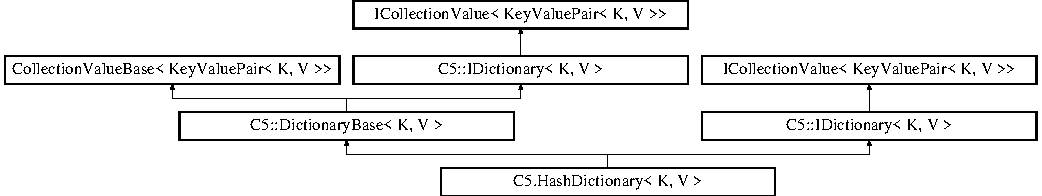
\includegraphics[height=2.629108cm]{class_c5_1_1_hash_dictionary}
\end{center}
\end{figure}
\subsection*{Public Member Functions}
\begin{DoxyCompactItemize}
\item 
\hyperlink{class_c5_1_1_hash_dictionary_a8cc5d148c92b62f69679cfdb20c14114}{Hash\+Dictionary} ()
\begin{DoxyCompactList}\small\item\em Create a hash dictionary using a default equality\+Comparer for the keys. Initial capacity of internal table will be 16 entries and threshold for expansion is 66\% fill. \end{DoxyCompactList}\item 
\hyperlink{class_c5_1_1_hash_dictionary_af4e45ac9fc7226b79a9cbf3d1d7014c4}{Hash\+Dictionary} (S\+C\+G.\+I\+Equality\+Comparer$<$ K $>$ keyequality\+Comparer)
\begin{DoxyCompactList}\small\item\em Create a hash dictionary using a custom equality\+Comparer for the keys. Initial capacity of internal table will be 16 entries and threshold for expansion is 66\% fill. \end{DoxyCompactList}\item 
\hyperlink{class_c5_1_1_hash_dictionary_a51e34dd05155273fc424ec3afbafedbe}{Hash\+Dictionary} (int capacity, double fill, S\+C\+G.\+I\+Equality\+Comparer$<$ K $>$ keyequality\+Comparer)
\begin{DoxyCompactList}\small\item\em Create a hash dictionary using a custom equality\+Comparer and prescribing the initial size of the dictionary and a non-\/default threshold for internal table expansion. \end{DoxyCompactList}\end{DoxyCompactItemize}
\subsection*{Additional Inherited Members}


\subsection{Detailed Description}
A generic dictionary class based on a hash set class T\+:\+C5.\+Hash\+Set`1. 



\subsection{Constructor \& Destructor Documentation}
\hypertarget{class_c5_1_1_hash_dictionary_a8cc5d148c92b62f69679cfdb20c14114}{}\index{C5\+::\+Hash\+Dictionary@{C5\+::\+Hash\+Dictionary}!Hash\+Dictionary@{Hash\+Dictionary}}
\index{Hash\+Dictionary@{Hash\+Dictionary}!C5\+::\+Hash\+Dictionary@{C5\+::\+Hash\+Dictionary}}
\subsubsection[{Hash\+Dictionary()}]{\setlength{\rightskip}{0pt plus 5cm}{\bf C5.\+Hash\+Dictionary}$<$ K, V $>$.{\bf Hash\+Dictionary} (
\begin{DoxyParamCaption}
{}
\end{DoxyParamCaption}
)}\label{class_c5_1_1_hash_dictionary_a8cc5d148c92b62f69679cfdb20c14114}


Create a hash dictionary using a default equality\+Comparer for the keys. Initial capacity of internal table will be 16 entries and threshold for expansion is 66\% fill. 

\hypertarget{class_c5_1_1_hash_dictionary_af4e45ac9fc7226b79a9cbf3d1d7014c4}{}\index{C5\+::\+Hash\+Dictionary@{C5\+::\+Hash\+Dictionary}!Hash\+Dictionary@{Hash\+Dictionary}}
\index{Hash\+Dictionary@{Hash\+Dictionary}!C5\+::\+Hash\+Dictionary@{C5\+::\+Hash\+Dictionary}}
\subsubsection[{Hash\+Dictionary(\+S\+C\+G.\+I\+Equality\+Comparer$<$ K $>$ keyequality\+Comparer)}]{\setlength{\rightskip}{0pt plus 5cm}{\bf C5.\+Hash\+Dictionary}$<$ K, V $>$.{\bf Hash\+Dictionary} (
\begin{DoxyParamCaption}
\item[{S\+C\+G.\+I\+Equality\+Comparer$<$ K $>$}]{keyequality\+Comparer}
\end{DoxyParamCaption}
)}\label{class_c5_1_1_hash_dictionary_af4e45ac9fc7226b79a9cbf3d1d7014c4}


Create a hash dictionary using a custom equality\+Comparer for the keys. Initial capacity of internal table will be 16 entries and threshold for expansion is 66\% fill. 


\begin{DoxyParams}{Parameters}
{\em keyequality\+Comparer} & The external key equality\+S\+C\+G.\+Comparer\\
\hline
\end{DoxyParams}
\hypertarget{class_c5_1_1_hash_dictionary_a51e34dd05155273fc424ec3afbafedbe}{}\index{C5\+::\+Hash\+Dictionary@{C5\+::\+Hash\+Dictionary}!Hash\+Dictionary@{Hash\+Dictionary}}
\index{Hash\+Dictionary@{Hash\+Dictionary}!C5\+::\+Hash\+Dictionary@{C5\+::\+Hash\+Dictionary}}
\subsubsection[{Hash\+Dictionary(int capacity, double fill, S\+C\+G.\+I\+Equality\+Comparer$<$ K $>$ keyequality\+Comparer)}]{\setlength{\rightskip}{0pt plus 5cm}{\bf C5.\+Hash\+Dictionary}$<$ K, V $>$.{\bf Hash\+Dictionary} (
\begin{DoxyParamCaption}
\item[{int}]{capacity, }
\item[{double}]{fill, }
\item[{S\+C\+G.\+I\+Equality\+Comparer$<$ K $>$}]{keyequality\+Comparer}
\end{DoxyParamCaption}
)}\label{class_c5_1_1_hash_dictionary_a51e34dd05155273fc424ec3afbafedbe}


Create a hash dictionary using a custom equality\+Comparer and prescribing the initial size of the dictionary and a non-\/default threshold for internal table expansion. 


\begin{DoxyParams}{Parameters}
{\em capacity} & The initial capacity. Will be rounded upwards to nearest power of 2, at least 16.\\
\hline
{\em fill} & The expansion threshold. Must be between 10\% and 90\%.\\
\hline
{\em keyequality\+Comparer} & The external key equality\+S\+C\+G.\+Comparer\\
\hline
\end{DoxyParams}


The documentation for this class was generated from the following file\+:\begin{DoxyCompactItemize}
\item 
C\+:/\+Users/rasmusl/\+Source/\+Repos/\+C5/\+C5/hashing/\hyperlink{_hash_dictionary_8cs}{Hash\+Dictionary.\+cs}\end{DoxyCompactItemize}

\hypertarget{class_c5_1_1_hashed_array_list}{}\section{C5.\+Hashed\+Array\+List$<$ T $>$ Class Template Reference}
\label{class_c5_1_1_hashed_array_list}\index{C5.\+Hashed\+Array\+List$<$ T $>$@{C5.\+Hashed\+Array\+List$<$ T $>$}}


A list collection based on a plain dynamic array data structure. Expansion of the internal array is performed by doubling on demand. The internal array is only shrinked by the Clear method.  


Inheritance diagram for C5.\+Hashed\+Array\+List$<$ T $>$\+:\begin{figure}[H]
\begin{center}
\leavevmode
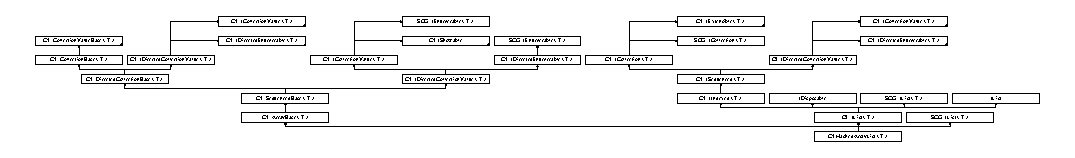
\includegraphics[height=1.673069cm]{class_c5_1_1_hashed_array_list}
\end{center}
\end{figure}
\subsection*{Public Member Functions}
\begin{DoxyCompactItemize}
\item 
\hyperlink{class_c5_1_1_hashed_array_list_a95961214ec0d64d96b0097c4631966d9}{Hashed\+Array\+List} ()
\begin{DoxyCompactList}\small\item\em Create an array list with default item equality\+Comparer and initial capacity 8 items. \end{DoxyCompactList}\item 
\hyperlink{class_c5_1_1_hashed_array_list_a5ffc18cd4def3f5032aca283876ad73d}{Hashed\+Array\+List} (S\+C\+G.\+I\+Equality\+Comparer$<$ T $>$ \hyperlink{class_c5_1_1_collection_base_a95e343400be0e8f3f8d6310f1aaf2cc6}{itemequality\+Comparer})
\begin{DoxyCompactList}\small\item\em Create an array list with external item equality\+Comparer and initial capacity 8 items. \end{DoxyCompactList}\item 
\hyperlink{class_c5_1_1_hashed_array_list_a413a70096e179f4a03411f8eecb60666}{Hashed\+Array\+List} (int capacity)
\begin{DoxyCompactList}\small\item\em Create an array list with default item equality\+Comparer and prescribed initial capacity. \end{DoxyCompactList}\item 
\hyperlink{class_c5_1_1_hashed_array_list_ad65f9dcc130e9c49c211cf2744c6c38d}{Hashed\+Array\+List} (int capacity, S\+C\+G.\+I\+Equality\+Comparer$<$ T $>$ \hyperlink{class_c5_1_1_collection_base_a95e343400be0e8f3f8d6310f1aaf2cc6}{itemequality\+Comparer})
\begin{DoxyCompactList}\small\item\em Create an array list with external item equality\+Comparer and prescribed initial capacity. \end{DoxyCompactList}\item 
virtual void \hyperlink{class_c5_1_1_hashed_array_list_a9d9c830e9b1746c5527cbc5172bb2a73}{Insert} (int index, T item)
\begin{DoxyCompactList}\small\item\em Insert an item at a specific index location in this list. /summary$>$ 
\begin{DoxyExceptions}{Exceptions}
{\em Index\+Out\+Of\+Range\+Exception} & if index is negative or $>$ the size of the collection. \\
\hline
{\em \hyperlink{class_c5_1_1_duplicate_not_allowed_exception}{Duplicate\+Not\+Allowed\+Exception}} & If the item is already present in the list.\\
\hline
\end{DoxyExceptions}

\begin{DoxyParams}{Parameters}
{\em index} & The index at which to insert.\\
\hline
{\em item} & The item to insert.\\
\hline
\end{DoxyParams}
\end{DoxyCompactList}\item 
void \hyperlink{class_c5_1_1_hashed_array_list_af2232ffdbc3b0970aeebcbda288f22c1}{Insert} (\hyperlink{interface_c5_1_1_i_list}{I\+List}$<$ T $>$ pointer, T item)
\begin{DoxyCompactList}\small\item\em Insert an item at the end of a compatible view, used as a pointer. \end{DoxyCompactList}\item 
virtual void \hyperlink{class_c5_1_1_hashed_array_list_a79d133efc3cafb5a74b265b0c85529f8}{Insert\+All} (int index, S\+C\+G.\+I\+Enumerable$<$ T $>$ items)
\begin{DoxyCompactList}\small\item\em Insert into this list all items from an enumerable collection starting at a particular index. \end{DoxyCompactList}\item 
virtual void \hyperlink{class_c5_1_1_hashed_array_list_a0466cbd0ea303e0ba40e8611dfa3f721}{Insert\+First} (T item)
\begin{DoxyCompactList}\small\item\em Insert an item at the front of this list; \end{DoxyCompactList}\item 
virtual void \hyperlink{class_c5_1_1_hashed_array_list_a616672c94355ca1f07af3a2b2ffe51bb}{Insert\+Last} (T item)
\begin{DoxyCompactList}\small\item\em Insert an item at the back of this list. \end{DoxyCompactList}\item 
virtual \hyperlink{interface_c5_1_1_i_list}{I\+List}$<$ T $>$ \hyperlink{class_c5_1_1_hashed_array_list_a44d89e2d1a233ee63a3e4efdee389585}{Find\+All} (Func$<$ T, bool $>$ filter)
\begin{DoxyCompactList}\small\item\em Create a new list consisting of the items of this list satisfying a certain predicate. \end{DoxyCompactList}\item 
virtual \hyperlink{interface_c5_1_1_i_list}{I\+List}$<$ V $>$ \hyperlink{class_c5_1_1_hashed_array_list_aacf59f051c56a96f62e5de97f1d51b87}{Map$<$ V $>$} (Func$<$ T, V $>$ mapper)
\begin{DoxyCompactList}\small\item\em Create a new list consisting of the results of mapping all items of this list. The new list will use the default item equality\+Comparer for the item type V. \end{DoxyCompactList}\item 
virtual \hyperlink{interface_c5_1_1_i_list}{I\+List}$<$ V $>$ \hyperlink{class_c5_1_1_hashed_array_list_a560e362c78363db5884315caaa4dd40a}{Map$<$ V $>$} (Func$<$ T, V $>$ mapper, S\+C\+G.\+I\+Equality\+Comparer$<$ V $>$ \hyperlink{class_c5_1_1_collection_base_a95e343400be0e8f3f8d6310f1aaf2cc6}{itemequality\+Comparer})
\begin{DoxyCompactList}\small\item\em Create a new list consisting of the results of mapping all items of this list. The new list will use a specified item equality\+Comparer for the item type. \end{DoxyCompactList}\item 
virtual T \hyperlink{class_c5_1_1_hashed_array_list_a36ab8321ad505bf9780d39a41d419f31}{Remove} ()
\begin{DoxyCompactList}\small\item\em Remove one item from the list\+: from the front if \end{DoxyCompactList}\item 
virtual T \hyperlink{class_c5_1_1_hashed_array_list_a569ec3b1a5fc7ab16bf6fc6eac5a2977}{Remove\+First} ()
\begin{DoxyCompactList}\small\item\em Remove one item from the fromnt of the list. \end{DoxyCompactList}\item 
virtual T \hyperlink{class_c5_1_1_hashed_array_list_a3d58befa5b2087abe708a3c76ecdda88}{Remove\+Last} ()
\begin{DoxyCompactList}\small\item\em Remove one item from the back of the list. \end{DoxyCompactList}\item 
virtual \hyperlink{interface_c5_1_1_i_list}{I\+List}$<$ T $>$ \hyperlink{class_c5_1_1_hashed_array_list_ad454b187e01388a575e68f6dfeb8c9b5}{View} (int start, int count)
\begin{DoxyCompactList}\small\item\em Create a list view on this list. \end{DoxyCompactList}\item 
virtual \hyperlink{interface_c5_1_1_i_list}{I\+List}$<$ T $>$ \hyperlink{class_c5_1_1_hashed_array_list_a3649fd58cf5e15c2ef488d61140895fd}{View\+Of} (T item)
\begin{DoxyCompactList}\small\item\em Create a list view on this list containing the (first) occurrence of a particular item. \end{DoxyCompactList}\item 
virtual \hyperlink{interface_c5_1_1_i_list}{I\+List}$<$ T $>$ \hyperlink{class_c5_1_1_hashed_array_list_a137af82d41074860aff0ccfaa67fac60}{Last\+View\+Of} (T item)
\begin{DoxyCompactList}\small\item\em Create a list view on this list containing the last occurrence of a particular item. \end{DoxyCompactList}\item 
virtual \hyperlink{interface_c5_1_1_i_list}{I\+List}$<$ T $>$ \hyperlink{class_c5_1_1_hashed_array_list_a0f24d23f3771a00a7e0d44da6de38932}{Slide} (int \hyperlink{class_c5_1_1_array_base_a2fff33ea372907c015262a3041b2f2af}{offset})
\begin{DoxyCompactList}\small\item\em Slide this list view along the underlying list. \end{DoxyCompactList}\item 
virtual \hyperlink{interface_c5_1_1_i_list}{I\+List}$<$ T $>$ \hyperlink{class_c5_1_1_hashed_array_list_a4b7f5fd43d17df77bded775e5d4ec6f6}{Slide} (int \hyperlink{class_c5_1_1_array_base_a2fff33ea372907c015262a3041b2f2af}{offset}, int \hyperlink{class_c5_1_1_collection_base_ab524b118754a5a8290b6528511272833}{size})
\begin{DoxyCompactList}\small\item\em Slide this list view along the underlying list, changing its size. \end{DoxyCompactList}\item 
virtual bool \hyperlink{class_c5_1_1_hashed_array_list_ae54510e056acda06d247570c08b72a4f}{Try\+Slide} (int \hyperlink{class_c5_1_1_array_base_a2fff33ea372907c015262a3041b2f2af}{offset})
\item 
virtual bool \hyperlink{class_c5_1_1_hashed_array_list_a443cbdd709e526aa841cb53518a2025c}{Try\+Slide} (int \hyperlink{class_c5_1_1_array_base_a2fff33ea372907c015262a3041b2f2af}{offset}, int \hyperlink{class_c5_1_1_collection_base_ab524b118754a5a8290b6528511272833}{size})
\item 
virtual \hyperlink{interface_c5_1_1_i_list}{I\+List}$<$ T $>$ \hyperlink{class_c5_1_1_hashed_array_list_a331f3c151db6a30da1bc11dbed9c3119}{Span} (\hyperlink{interface_c5_1_1_i_list}{I\+List}$<$ T $>$ other\+View)
\item 
virtual void \hyperlink{class_c5_1_1_hashed_array_list_a79bae38c188939659db04f3a90869122}{Reverse} ()
\begin{DoxyCompactList}\small\item\em Reverst the list so the items are in the opposite sequence order. \end{DoxyCompactList}\item 
bool \hyperlink{class_c5_1_1_hashed_array_list_a7d8165aa133bc45c19481e7d74d2ceb7}{Is\+Sorted} ()
\begin{DoxyCompactList}\small\item\em Check if this list is sorted according to the default sorting order for the item type T, as defined by the T\+:\+C5.\+Comparer`1 class \end{DoxyCompactList}\item 
virtual bool \hyperlink{class_c5_1_1_hashed_array_list_a4ad671797c33a01e7faf008c184bfdc6}{Is\+Sorted} (S\+C\+G.\+I\+Comparer$<$ T $>$ c)
\begin{DoxyCompactList}\small\item\em Check if this list is sorted according to a specific sorting order. \end{DoxyCompactList}\item 
virtual void \hyperlink{class_c5_1_1_hashed_array_list_a8e3acdf07e2b45b9e1be1a1774edbfb9}{Sort} ()
\begin{DoxyCompactList}\small\item\em Sort the items of the list according to the default sorting order for the item type T, as defined by the Comparer\mbox{[}T\mbox{]} class (T\+:\+C5.\+Comparer`1). \end{DoxyCompactList}\item 
virtual void \hyperlink{class_c5_1_1_hashed_array_list_a3e2208ed8af4641d9e9ce503e43066c7}{Sort} (S\+C\+G.\+I\+Comparer$<$ T $>$ comparer)
\begin{DoxyCompactList}\small\item\em Sort the items of the list according to a specific sorting order. \end{DoxyCompactList}\item 
virtual void \hyperlink{class_c5_1_1_hashed_array_list_add0d88b73c89c2262c39e7b117acc4a2}{Shuffle} ()
\begin{DoxyCompactList}\small\item\em Randomly shuffle the items of this list. \end{DoxyCompactList}\item 
virtual void \hyperlink{class_c5_1_1_hashed_array_list_a8cb8a5ae24eddc8d343ef054b0f86dcd}{Shuffle} (Random rnd)
\begin{DoxyCompactList}\small\item\em Shuffle the items of this list according to a specific random source. \end{DoxyCompactList}\item 
virtual int \hyperlink{class_c5_1_1_hashed_array_list_a6d13105e7f303fc04310801abed22946}{Index\+Of} (T item)
\begin{DoxyCompactList}\small\item\em Search for an item in the list going forwrds from the start. \end{DoxyCompactList}\item 
virtual int \hyperlink{class_c5_1_1_hashed_array_list_a6fff76a2253ec4f3fb52abcddecbc52c}{Last\+Index\+Of} (T item)
\begin{DoxyCompactList}\small\item\em Search for an item in the list going backwords from the end. \end{DoxyCompactList}\item 
virtual T \hyperlink{class_c5_1_1_hashed_array_list_a28dadd5b31e5daa8eb34728f0c31728a}{Remove\+At} (int index)
\begin{DoxyCompactList}\small\item\em Remove the item at a specific position of the list. \end{DoxyCompactList}\item 
virtual void \hyperlink{class_c5_1_1_hashed_array_list_ab443d1ea4dd141b18debf8d450deb2fb}{Remove\+Interval} (int start, int count)
\begin{DoxyCompactList}\small\item\em Remove all items in an index interval. \end{DoxyCompactList}\item 
override int \hyperlink{class_c5_1_1_hashed_array_list_a8f23bbdc50d2c951e19fad0008f2f25a}{Get\+Unsequenced\+Hash\+Code} ()
\item 
override bool \hyperlink{class_c5_1_1_hashed_array_list_a6ed6c87e49b97c50d2cafba6fe050b26}{Unsequenced\+Equals} (\hyperlink{interface_c5_1_1_i_collection}{I\+Collection}$<$ T $>$ that)
\item 
virtual bool \hyperlink{class_c5_1_1_hashed_array_list_a4b108299a930ceaecd8484023a656cf4}{Contains} (T item)
\begin{DoxyCompactList}\small\item\em Check if this collection contains (an item equivalent to according to the itemequality\+Comparer) a particular value. \end{DoxyCompactList}\item 
virtual bool \hyperlink{class_c5_1_1_hashed_array_list_ac29e24d17686e2c3998a590a60b27d71}{Find} (ref T item)
\begin{DoxyCompactList}\small\item\em Check if this collection contains an item equivalent according to the itemequality\+Comparer to a particular value. If so, return in the ref argument (a binary copy of) the actual value found. \end{DoxyCompactList}\item 
virtual bool \hyperlink{class_c5_1_1_hashed_array_list_a265287f01f52f2975ffdc926af3e8998}{Update} (T item)
\begin{DoxyCompactList}\small\item\em Check if this collection contains an item equivalent according to the itemequality\+Comparer to a particular value. If so, update the item in the collection to with a binary copy of the supplied value. This will only update the first mathching item. \end{DoxyCompactList}\item 
virtual bool \hyperlink{class_c5_1_1_hashed_array_list_a68f51b76c891c44cd424c7604cef85ab}{Update} (T item, out T olditem)
\item 
virtual bool \hyperlink{class_c5_1_1_hashed_array_list_a7adaad90a9e57a90c3bc197dc4d1289c}{Find\+Or\+Add} (ref T item)
\begin{DoxyCompactList}\small\item\em Check if this collection contains an item equivalent according to the itemequality\+Comparer to a particular value. If so, return in the ref argument (a binary copy of) the actual value found. Else, add the item to the collection. \end{DoxyCompactList}\item 
virtual bool \hyperlink{class_c5_1_1_hashed_array_list_a97e9d72944cb3ff6b5d5162e381e36e7}{Update\+Or\+Add} (T item)
\begin{DoxyCompactList}\small\item\em Check if this collection contains an item equivalent according to the itemequality\+Comparer to a particular value. If so, update the item in the collection to with a binary copy of the supplied value. This will only update the first mathching item. \end{DoxyCompactList}\item 
virtual bool \hyperlink{class_c5_1_1_hashed_array_list_ac0be87fa58015a3191d91ab0e8c75766}{Update\+Or\+Add} (T item, out T olditem)
\item 
virtual bool \hyperlink{class_c5_1_1_hashed_array_list_a4453b3955bce1670914b4aa2f469b4c0}{Remove} (T item)
\begin{DoxyCompactList}\small\item\em Remove a particular item from this list. The item will be searched for from the end of the list if \end{DoxyCompactList}\item 
virtual bool \hyperlink{class_c5_1_1_hashed_array_list_aaf108802a6f4024858b9d178109126ee}{Remove} (T item, out T removeditem)
\begin{DoxyCompactList}\small\item\em Remove the first copy of a particular item from this collection if found. If an item was removed, report a binary copy of the actual item removed in the argument. The item will be searched for from the end of the list if \end{DoxyCompactList}\item 
virtual void \hyperlink{class_c5_1_1_hashed_array_list_a9598f605bb5e2de9f4a1bfce80a0dd0b}{Remove\+All} (S\+C\+G.\+I\+Enumerable$<$ T $>$ items)
\begin{DoxyCompactList}\small\item\em Remove all items in another collection from this one, taking multiplicities into account. Matching items will be removed from the front. Current implementation is not optimal. \end{DoxyCompactList}\item 
override void \hyperlink{class_c5_1_1_hashed_array_list_aeca323e5f962607ee4384549aaba5d28}{Clear} ()
\begin{DoxyCompactList}\small\item\em Remove all items from this collection, resetting internal array size. \end{DoxyCompactList}\item 
virtual void \hyperlink{class_c5_1_1_hashed_array_list_a2c474cfc8e742163eec9bfba91169a79}{Retain\+All} (S\+C\+G.\+I\+Enumerable$<$ T $>$ items)
\begin{DoxyCompactList}\small\item\em Remove all items not in some other collection from this one, taking multiplicities into account. Items are retained front first. \end{DoxyCompactList}\item 
virtual bool \hyperlink{class_c5_1_1_hashed_array_list_ae3145f69b175e6b3d9af471b3ef89c80}{Contains\+All} (S\+C\+G.\+I\+Enumerable$<$ T $>$ items)
\begin{DoxyCompactList}\small\item\em Check if this collection contains all the values in another collection, taking multiplicities into account. Current implementation is not optimal. \end{DoxyCompactList}\item 
virtual int \hyperlink{class_c5_1_1_hashed_array_list_a4fb06172f38039104765ee9d6ed78842}{Contains\+Count} (T item)
\begin{DoxyCompactList}\small\item\em Count the number of items of the collection equal to a particular value. Returns 0 if and only if the value is not in the collection. \end{DoxyCompactList}\item 
virtual \hyperlink{interface_c5_1_1_i_collection_value}{I\+Collection\+Value}$<$ T $>$ \hyperlink{class_c5_1_1_hashed_array_list_ab51e4a315e9d2a09ff389f64bc7a13a1}{Unique\+Items} ()
\item 
virtual \hyperlink{interface_c5_1_1_i_collection_value}{I\+Collection\+Value}$<$ \hyperlink{struct_c5_1_1_key_value_pair}{Key\+Value\+Pair}$<$ T, int $>$ $>$ \hyperlink{class_c5_1_1_hashed_array_list_a8a36b62fa880e713de8e5d8ccfd19595}{Item\+Multiplicities} ()
\item 
virtual void \hyperlink{class_c5_1_1_hashed_array_list_a5b7779ece9c62551eb1c1a24c53906a5}{Remove\+All\+Copies} (T item)
\begin{DoxyCompactList}\small\item\em Remove all items equal to a given one. \end{DoxyCompactList}\item 
override bool \hyperlink{class_c5_1_1_hashed_array_list_aed94ab3e8f52b3cd4b7825b12d6876b2}{Check} ()
\begin{DoxyCompactList}\small\item\em Check the integrity of the internal data structures of this array list. \end{DoxyCompactList}\item 
virtual bool \hyperlink{class_c5_1_1_hashed_array_list_a4606087ab02e09f75ce6810b7a9d11a4}{Add} (T item)
\begin{DoxyCompactList}\small\item\em Add an item to end of this list. \end{DoxyCompactList}\item 
virtual void \hyperlink{class_c5_1_1_hashed_array_list_acf2afaacbfe8474425f2840af10118a3}{Add\+All} (S\+C\+G.\+I\+Enumerable$<$ T $>$ items)
\begin{DoxyCompactList}\small\item\em Add the elements from another collection to this collection. \end{DoxyCompactList}\item 
override S\+C\+G.\+I\+Enumerator$<$ T $>$ \hyperlink{class_c5_1_1_hashed_array_list_a0ce81bee1c45ccbc3105698a4f4692a8}{Get\+Enumerator} ()
\begin{DoxyCompactList}\small\item\em Create an enumerator for the collection \end{DoxyCompactList}\item 
virtual void \hyperlink{class_c5_1_1_hashed_array_list_aa8f55429bbf1b548fdb698740ea4d94c}{Dispose} ()
\begin{DoxyCompactList}\small\item\em Invalidate this list. If a view, just invalidate the view. If not a view, invalidate the list and all views on it. \end{DoxyCompactList}\end{DoxyCompactItemize}
\subsection*{Protected Member Functions}
\begin{DoxyCompactItemize}
\item 
override void \hyperlink{class_c5_1_1_hashed_array_list_a4dce92728aada5e2d56902d0565247ff}{expand} ()
\begin{DoxyCompactList}\small\item\em Double the size of the internal array. \end{DoxyCompactList}\item 
override void \hyperlink{class_c5_1_1_hashed_array_list_ae227e09958e8ce6eea7e0132ecd1a6aa}{expand} (int newcapacity, int newsize)
\begin{DoxyCompactList}\small\item\em Expand the internal array, resetting the index of the first unused element. \end{DoxyCompactList}\item 
override void \hyperlink{class_c5_1_1_hashed_array_list_a4a91454e022d105216e78756eff729c9}{updatecheck} ()
\begin{DoxyCompactList}\small\item\em Check if it is valid to perform updates and increment stamp if so. \end{DoxyCompactList}\item 
override void \hyperlink{class_c5_1_1_hashed_array_list_a0d8db9ef70c6d213b8c4f9302d9d1c15}{modifycheck} (int \hyperlink{class_c5_1_1_collection_base_ae13bd5b482306a49a4d10654a9b8b064}{stamp})
\begin{DoxyCompactList}\small\item\em Check that the list has not been updated since a particular time. \end{DoxyCompactList}\item 
override void \hyperlink{class_c5_1_1_hashed_array_list_a70d3534f5dcf4e6b4c041ffc58dbc830}{insert} (int i, T item)
\begin{DoxyCompactList}\small\item\em Internal version of Insert with no modification checks. \end{DoxyCompactList}\end{DoxyCompactItemize}
\subsection*{Properties}
\begin{DoxyCompactItemize}
\item 
override \hyperlink{namespace_c5_a9143bfd561fffa025d21561674758008}{Event\+Type\+Enum} \hyperlink{class_c5_1_1_hashed_array_list_accdd1813a4a5bdff31d1e19d9867c868}{Listenable\+Events}\hspace{0.3cm}{\ttfamily  \mbox{[}get\mbox{]}}
\item 
virtual T \hyperlink{class_c5_1_1_hashed_array_list_af6ac7881402fcbbbadadd1b1e2f22478}{First}\hspace{0.3cm}{\ttfamily  \mbox{[}get\mbox{]}}
\item 
virtual T \hyperlink{class_c5_1_1_hashed_array_list_aaa8c79aed9aec799ea687392fc39a028}{Last}\hspace{0.3cm}{\ttfamily  \mbox{[}get\mbox{]}}
\item 
virtual bool \hyperlink{class_c5_1_1_hashed_array_list_afc96d23115af14b75b10a1b9af9e844c}{F\+I\+F\+O}\hspace{0.3cm}{\ttfamily  \mbox{[}get, set\mbox{]}}
\begin{DoxyCompactList}\small\item\em Since \end{DoxyCompactList}\item 
virtual bool \hyperlink{class_c5_1_1_hashed_array_list_a9cdc553cbda54a181c5c00257b3b6486}{Is\+Fixed\+Size}\hspace{0.3cm}{\ttfamily  \mbox{[}get\mbox{]}}
\item 
virtual T \hyperlink{class_c5_1_1_hashed_array_list_a7122ca8cf35c8a9ec72facf36d2fb360}{this\mbox{[}int index\mbox{]}}\hspace{0.3cm}{\ttfamily  \mbox{[}get, set\mbox{]}}
\begin{DoxyCompactList}\small\item\em On this list, this indexer is read/write. \end{DoxyCompactList}\item 
virtual \hyperlink{namespace_c5_a615ba88dcdaa8d5a3c5f833a73d7fad6}{Speed} \hyperlink{class_c5_1_1_hashed_array_list_a60504efec769c7c3d326c5770bd2cd7e}{Indexing\+Speed}\hspace{0.3cm}{\ttfamily  \mbox{[}get\mbox{]}}
\item 
virtual \hyperlink{interface_c5_1_1_i_list}{I\+List}$<$ T $>$ \hyperlink{class_c5_1_1_hashed_array_list_aa8039fdbfaa6caa1b0f2b4364a43e292}{Underlying}\hspace{0.3cm}{\ttfamily  \mbox{[}get\mbox{]}}
\begin{DoxyCompactList}\small\item\em Null if this list is not a view. \end{DoxyCompactList}\item 
virtual int \hyperlink{class_c5_1_1_hashed_array_list_a1fb3ecd68335ab401853035b171b9510}{Offset}\hspace{0.3cm}{\ttfamily  \mbox{[}get\mbox{]}}
\item 
virtual bool \hyperlink{class_c5_1_1_hashed_array_list_a159bd9790dc21d807212e206bd0defeb}{Is\+Valid}\hspace{0.3cm}{\ttfamily  \mbox{[}get\mbox{]}}
\item 
virtual \hyperlink{namespace_c5_a615ba88dcdaa8d5a3c5f833a73d7fad6}{Speed} \hyperlink{class_c5_1_1_hashed_array_list_adabe67b56cee8665745ded62f5bb5528}{Contains\+Speed}\hspace{0.3cm}{\ttfamily  \mbox{[}get\mbox{]}}
\begin{DoxyCompactList}\small\item\em The value is symbolic indicating the type of asymptotic complexity in terms of the size of this collection (worst-\/case or amortized as relevant). \end{DoxyCompactList}\item 
virtual bool \hyperlink{class_c5_1_1_hashed_array_list_ae848f960fa4fd6356992dae988b66ca3}{Allows\+Duplicates}\hspace{0.3cm}{\ttfamily  \mbox{[}get\mbox{]}}
\item 
virtual bool \hyperlink{class_c5_1_1_hashed_array_list_a12f8301ee0eb89f4f25508a6e22e0105}{Duplicates\+By\+Counting}\hspace{0.3cm}{\ttfamily  \mbox{[}get\mbox{]}}
\begin{DoxyCompactList}\small\item\em By convention this is true for any collection with set semantics. \end{DoxyCompactList}\item 
override int \hyperlink{class_c5_1_1_hashed_array_list_a46e32f347ac0e80756fdc98970424e8b}{Count}\hspace{0.3cm}{\ttfamily  \mbox{[}get\mbox{]}}
\end{DoxyCompactItemize}
\subsection*{Additional Inherited Members}


\subsection{Detailed Description}
A list collection based on a plain dynamic array data structure. Expansion of the internal array is performed by doubling on demand. The internal array is only shrinked by the Clear method. 

{\itshape When the F\+I\+F\+O property is set to false this class works fine as a stack of T. When the F\+I\+F\+O property is set to true the class will function as a (F\+I\+F\+O) queue but very inefficiently, use a \hyperlink{class_c5_1_1_linked_list}{Linked\+List} (T\+:\+C5.\+Linked\+List`1) instead.} 

\subsection{Constructor \& Destructor Documentation}
\hypertarget{class_c5_1_1_hashed_array_list_a95961214ec0d64d96b0097c4631966d9}{}\index{C5\+::\+Hashed\+Array\+List@{C5\+::\+Hashed\+Array\+List}!Hashed\+Array\+List@{Hashed\+Array\+List}}
\index{Hashed\+Array\+List@{Hashed\+Array\+List}!C5\+::\+Hashed\+Array\+List@{C5\+::\+Hashed\+Array\+List}}
\subsubsection[{Hashed\+Array\+List()}]{\setlength{\rightskip}{0pt plus 5cm}{\bf C5.\+Hashed\+Array\+List}$<$ T $>$.{\bf Hashed\+Array\+List} (
\begin{DoxyParamCaption}
{}
\end{DoxyParamCaption}
)}\label{class_c5_1_1_hashed_array_list_a95961214ec0d64d96b0097c4631966d9}


Create an array list with default item equality\+Comparer and initial capacity 8 items. 

\hypertarget{class_c5_1_1_hashed_array_list_a5ffc18cd4def3f5032aca283876ad73d}{}\index{C5\+::\+Hashed\+Array\+List@{C5\+::\+Hashed\+Array\+List}!Hashed\+Array\+List@{Hashed\+Array\+List}}
\index{Hashed\+Array\+List@{Hashed\+Array\+List}!C5\+::\+Hashed\+Array\+List@{C5\+::\+Hashed\+Array\+List}}
\subsubsection[{Hashed\+Array\+List(\+S\+C\+G.\+I\+Equality\+Comparer$<$ T $>$ itemequality\+Comparer)}]{\setlength{\rightskip}{0pt plus 5cm}{\bf C5.\+Hashed\+Array\+List}$<$ T $>$.{\bf Hashed\+Array\+List} (
\begin{DoxyParamCaption}
\item[{S\+C\+G.\+I\+Equality\+Comparer$<$ T $>$}]{itemequality\+Comparer}
\end{DoxyParamCaption}
)}\label{class_c5_1_1_hashed_array_list_a5ffc18cd4def3f5032aca283876ad73d}


Create an array list with external item equality\+Comparer and initial capacity 8 items. 


\begin{DoxyParams}{Parameters}
{\em itemequality\+Comparer} & The external item equality\+S\+C\+G.\+Comparer\\
\hline
\end{DoxyParams}
\hypertarget{class_c5_1_1_hashed_array_list_a413a70096e179f4a03411f8eecb60666}{}\index{C5\+::\+Hashed\+Array\+List@{C5\+::\+Hashed\+Array\+List}!Hashed\+Array\+List@{Hashed\+Array\+List}}
\index{Hashed\+Array\+List@{Hashed\+Array\+List}!C5\+::\+Hashed\+Array\+List@{C5\+::\+Hashed\+Array\+List}}
\subsubsection[{Hashed\+Array\+List(int capacity)}]{\setlength{\rightskip}{0pt plus 5cm}{\bf C5.\+Hashed\+Array\+List}$<$ T $>$.{\bf Hashed\+Array\+List} (
\begin{DoxyParamCaption}
\item[{int}]{capacity}
\end{DoxyParamCaption}
)}\label{class_c5_1_1_hashed_array_list_a413a70096e179f4a03411f8eecb60666}


Create an array list with default item equality\+Comparer and prescribed initial capacity. 


\begin{DoxyParams}{Parameters}
{\em capacity} & The prescribed capacity\\
\hline
\end{DoxyParams}
\hypertarget{class_c5_1_1_hashed_array_list_ad65f9dcc130e9c49c211cf2744c6c38d}{}\index{C5\+::\+Hashed\+Array\+List@{C5\+::\+Hashed\+Array\+List}!Hashed\+Array\+List@{Hashed\+Array\+List}}
\index{Hashed\+Array\+List@{Hashed\+Array\+List}!C5\+::\+Hashed\+Array\+List@{C5\+::\+Hashed\+Array\+List}}
\subsubsection[{Hashed\+Array\+List(int capacity, S\+C\+G.\+I\+Equality\+Comparer$<$ T $>$ itemequality\+Comparer)}]{\setlength{\rightskip}{0pt plus 5cm}{\bf C5.\+Hashed\+Array\+List}$<$ T $>$.{\bf Hashed\+Array\+List} (
\begin{DoxyParamCaption}
\item[{int}]{capacity, }
\item[{S\+C\+G.\+I\+Equality\+Comparer$<$ T $>$}]{itemequality\+Comparer}
\end{DoxyParamCaption}
)}\label{class_c5_1_1_hashed_array_list_ad65f9dcc130e9c49c211cf2744c6c38d}


Create an array list with external item equality\+Comparer and prescribed initial capacity. 


\begin{DoxyParams}{Parameters}
{\em capacity} & The prescribed capacity\\
\hline
{\em itemequality\+Comparer} & The external item equality\+S\+C\+G.\+Comparer\\
\hline
\end{DoxyParams}


\subsection{Member Function Documentation}
\hypertarget{class_c5_1_1_hashed_array_list_a4606087ab02e09f75ce6810b7a9d11a4}{}\index{C5\+::\+Hashed\+Array\+List@{C5\+::\+Hashed\+Array\+List}!Add@{Add}}
\index{Add@{Add}!C5\+::\+Hashed\+Array\+List@{C5\+::\+Hashed\+Array\+List}}
\subsubsection[{Add(\+T item)}]{\setlength{\rightskip}{0pt plus 5cm}virtual bool {\bf C5.\+Hashed\+Array\+List}$<$ T $>$.Add (
\begin{DoxyParamCaption}
\item[{T}]{item}
\end{DoxyParamCaption}
)\hspace{0.3cm}{\ttfamily [virtual]}}\label{class_c5_1_1_hashed_array_list_a4606087ab02e09f75ce6810b7a9d11a4}


Add an item to end of this list. 


\begin{DoxyParams}{Parameters}
{\em item} & The item to add.\\
\hline
\end{DoxyParams}
\begin{DoxyReturn}{Returns}
True
\end{DoxyReturn}


Implements \hyperlink{interface_c5_1_1_i_list_a800000d7344d000c1b8c67acda464a3d}{C5.\+I\+List$<$ T $>$}.

\hypertarget{class_c5_1_1_hashed_array_list_acf2afaacbfe8474425f2840af10118a3}{}\index{C5\+::\+Hashed\+Array\+List@{C5\+::\+Hashed\+Array\+List}!Add\+All@{Add\+All}}
\index{Add\+All@{Add\+All}!C5\+::\+Hashed\+Array\+List@{C5\+::\+Hashed\+Array\+List}}
\subsubsection[{Add\+All(\+S\+C\+G.\+I\+Enumerable$<$ T $>$ items)}]{\setlength{\rightskip}{0pt plus 5cm}virtual void {\bf C5.\+Hashed\+Array\+List}$<$ T $>$.Add\+All (
\begin{DoxyParamCaption}
\item[{S\+C\+G.\+I\+Enumerable$<$ T $>$}]{items}
\end{DoxyParamCaption}
)\hspace{0.3cm}{\ttfamily [virtual]}}\label{class_c5_1_1_hashed_array_list_acf2afaacbfe8474425f2840af10118a3}


Add the elements from another collection to this collection. 


\begin{DoxyParams}{Parameters}
{\em items} & \\
\hline
\end{DoxyParams}


Implements \hyperlink{interface_c5_1_1_i_extensible_a1fb4d50c5b340e60303da72e9d0ede6e}{C5.\+I\+Extensible$<$ T $>$}.

\hypertarget{class_c5_1_1_hashed_array_list_aed94ab3e8f52b3cd4b7825b12d6876b2}{}\index{C5\+::\+Hashed\+Array\+List@{C5\+::\+Hashed\+Array\+List}!Check@{Check}}
\index{Check@{Check}!C5\+::\+Hashed\+Array\+List@{C5\+::\+Hashed\+Array\+List}}
\subsubsection[{Check()}]{\setlength{\rightskip}{0pt plus 5cm}override bool {\bf C5.\+Hashed\+Array\+List}$<$ T $>$.Check (
\begin{DoxyParamCaption}
{}
\end{DoxyParamCaption}
)\hspace{0.3cm}{\ttfamily [virtual]}}\label{class_c5_1_1_hashed_array_list_aed94ab3e8f52b3cd4b7825b12d6876b2}


Check the integrity of the internal data structures of this array list. 

\begin{DoxyReturn}{Returns}
True if check does not fail.
\end{DoxyReturn}


Reimplemented from \hyperlink{class_c5_1_1_array_base_a45363fe7b6709bba1e37094d2cd5bfdf}{C5.\+Array\+Base$<$ T $>$}.

\hypertarget{class_c5_1_1_hashed_array_list_aeca323e5f962607ee4384549aaba5d28}{}\index{C5\+::\+Hashed\+Array\+List@{C5\+::\+Hashed\+Array\+List}!Clear@{Clear}}
\index{Clear@{Clear}!C5\+::\+Hashed\+Array\+List@{C5\+::\+Hashed\+Array\+List}}
\subsubsection[{Clear()}]{\setlength{\rightskip}{0pt plus 5cm}override void {\bf C5.\+Hashed\+Array\+List}$<$ T $>$.Clear (
\begin{DoxyParamCaption}
{}
\end{DoxyParamCaption}
)\hspace{0.3cm}{\ttfamily [virtual]}}\label{class_c5_1_1_hashed_array_list_aeca323e5f962607ee4384549aaba5d28}


Remove all items from this collection, resetting internal array size. 



Reimplemented from \hyperlink{class_c5_1_1_array_base_abfee2ce913abdf40245562982f40a496}{C5.\+Array\+Base$<$ T $>$}.

\hypertarget{class_c5_1_1_hashed_array_list_a4b108299a930ceaecd8484023a656cf4}{}\index{C5\+::\+Hashed\+Array\+List@{C5\+::\+Hashed\+Array\+List}!Contains@{Contains}}
\index{Contains@{Contains}!C5\+::\+Hashed\+Array\+List@{C5\+::\+Hashed\+Array\+List}}
\subsubsection[{Contains(\+T item)}]{\setlength{\rightskip}{0pt plus 5cm}virtual bool {\bf C5.\+Hashed\+Array\+List}$<$ T $>$.Contains (
\begin{DoxyParamCaption}
\item[{T}]{item}
\end{DoxyParamCaption}
)\hspace{0.3cm}{\ttfamily [virtual]}}\label{class_c5_1_1_hashed_array_list_a4b108299a930ceaecd8484023a656cf4}


Check if this collection contains (an item equivalent to according to the itemequality\+Comparer) a particular value. 


\begin{DoxyParams}{Parameters}
{\em item} & The value to check for.\\
\hline
\end{DoxyParams}
\begin{DoxyReturn}{Returns}
True if the items is in this collection.
\end{DoxyReturn}


Implements \hyperlink{interface_c5_1_1_i_list_a108b607b042959d063e1ca77e242406c}{C5.\+I\+List$<$ T $>$}.

\hypertarget{class_c5_1_1_hashed_array_list_ae3145f69b175e6b3d9af471b3ef89c80}{}\index{C5\+::\+Hashed\+Array\+List@{C5\+::\+Hashed\+Array\+List}!Contains\+All@{Contains\+All}}
\index{Contains\+All@{Contains\+All}!C5\+::\+Hashed\+Array\+List@{C5\+::\+Hashed\+Array\+List}}
\subsubsection[{Contains\+All(\+S\+C\+G.\+I\+Enumerable$<$ T $>$ items)}]{\setlength{\rightskip}{0pt plus 5cm}virtual bool {\bf C5.\+Hashed\+Array\+List}$<$ T $>$.Contains\+All (
\begin{DoxyParamCaption}
\item[{S\+C\+G.\+I\+Enumerable$<$ T $>$}]{items}
\end{DoxyParamCaption}
)\hspace{0.3cm}{\ttfamily [virtual]}}\label{class_c5_1_1_hashed_array_list_ae3145f69b175e6b3d9af471b3ef89c80}


Check if this collection contains all the values in another collection, taking multiplicities into account. Current implementation is not optimal. 


\begin{DoxyParams}{Parameters}
{\em items} & The \\
\hline
\end{DoxyParams}
\begin{DoxyReturn}{Returns}
True if all values in 
\begin{DoxyCode}
items
\end{DoxyCode}
is in this collection.
\end{DoxyReturn}


Implements \hyperlink{interface_c5_1_1_i_collection_a93abf02183a46f56af8d90f1d69982a8}{C5.\+I\+Collection$<$ T $>$}.

\hypertarget{class_c5_1_1_hashed_array_list_a4fb06172f38039104765ee9d6ed78842}{}\index{C5\+::\+Hashed\+Array\+List@{C5\+::\+Hashed\+Array\+List}!Contains\+Count@{Contains\+Count}}
\index{Contains\+Count@{Contains\+Count}!C5\+::\+Hashed\+Array\+List@{C5\+::\+Hashed\+Array\+List}}
\subsubsection[{Contains\+Count(\+T item)}]{\setlength{\rightskip}{0pt plus 5cm}virtual int {\bf C5.\+Hashed\+Array\+List}$<$ T $>$.Contains\+Count (
\begin{DoxyParamCaption}
\item[{T}]{item}
\end{DoxyParamCaption}
)\hspace{0.3cm}{\ttfamily [virtual]}}\label{class_c5_1_1_hashed_array_list_a4fb06172f38039104765ee9d6ed78842}


Count the number of items of the collection equal to a particular value. Returns 0 if and only if the value is not in the collection. 


\begin{DoxyParams}{Parameters}
{\em item} & The value to count.\\
\hline
\end{DoxyParams}
\begin{DoxyReturn}{Returns}
The number of copies found.
\end{DoxyReturn}


Implements \hyperlink{interface_c5_1_1_i_collection_acfe7e2c9b14c384762269edbb57b7fbe}{C5.\+I\+Collection$<$ T $>$}.

\hypertarget{class_c5_1_1_hashed_array_list_aa8f55429bbf1b548fdb698740ea4d94c}{}\index{C5\+::\+Hashed\+Array\+List@{C5\+::\+Hashed\+Array\+List}!Dispose@{Dispose}}
\index{Dispose@{Dispose}!C5\+::\+Hashed\+Array\+List@{C5\+::\+Hashed\+Array\+List}}
\subsubsection[{Dispose()}]{\setlength{\rightskip}{0pt plus 5cm}virtual void {\bf C5.\+Hashed\+Array\+List}$<$ T $>$.Dispose (
\begin{DoxyParamCaption}
{}
\end{DoxyParamCaption}
)\hspace{0.3cm}{\ttfamily [virtual]}}\label{class_c5_1_1_hashed_array_list_aa8f55429bbf1b548fdb698740ea4d94c}


Invalidate this list. If a view, just invalidate the view. If not a view, invalidate the list and all views on it. 

\hypertarget{class_c5_1_1_hashed_array_list_a4dce92728aada5e2d56902d0565247ff}{}\index{C5\+::\+Hashed\+Array\+List@{C5\+::\+Hashed\+Array\+List}!expand@{expand}}
\index{expand@{expand}!C5\+::\+Hashed\+Array\+List@{C5\+::\+Hashed\+Array\+List}}
\subsubsection[{expand()}]{\setlength{\rightskip}{0pt plus 5cm}override void {\bf C5.\+Hashed\+Array\+List}$<$ T $>$.expand (
\begin{DoxyParamCaption}
{}
\end{DoxyParamCaption}
)\hspace{0.3cm}{\ttfamily [protected]}, {\ttfamily [virtual]}}\label{class_c5_1_1_hashed_array_list_a4dce92728aada5e2d56902d0565247ff}


Double the size of the internal array. 



Reimplemented from \hyperlink{class_c5_1_1_array_base_a6e32bc0bafd9263e2ccb18a5fedb032d}{C5.\+Array\+Base$<$ T $>$}.

\hypertarget{class_c5_1_1_hashed_array_list_ae227e09958e8ce6eea7e0132ecd1a6aa}{}\index{C5\+::\+Hashed\+Array\+List@{C5\+::\+Hashed\+Array\+List}!expand@{expand}}
\index{expand@{expand}!C5\+::\+Hashed\+Array\+List@{C5\+::\+Hashed\+Array\+List}}
\subsubsection[{expand(int newcapacity, int newsize)}]{\setlength{\rightskip}{0pt plus 5cm}override void {\bf C5.\+Hashed\+Array\+List}$<$ T $>$.expand (
\begin{DoxyParamCaption}
\item[{int}]{newcapacity, }
\item[{int}]{newsize}
\end{DoxyParamCaption}
)\hspace{0.3cm}{\ttfamily [protected]}, {\ttfamily [virtual]}}\label{class_c5_1_1_hashed_array_list_ae227e09958e8ce6eea7e0132ecd1a6aa}


Expand the internal array, resetting the index of the first unused element. 


\begin{DoxyParams}{Parameters}
{\em newcapacity} & The new capacity (will be rouded upwards to a power of 2).\\
\hline
{\em newsize} & The new count of \\
\hline
\end{DoxyParams}


Reimplemented from \hyperlink{class_c5_1_1_array_base_a5f2dcfe8c4c68077aa1b6c80a2d179c6}{C5.\+Array\+Base$<$ T $>$}.

\hypertarget{class_c5_1_1_hashed_array_list_ac29e24d17686e2c3998a590a60b27d71}{}\index{C5\+::\+Hashed\+Array\+List@{C5\+::\+Hashed\+Array\+List}!Find@{Find}}
\index{Find@{Find}!C5\+::\+Hashed\+Array\+List@{C5\+::\+Hashed\+Array\+List}}
\subsubsection[{Find(ref T item)}]{\setlength{\rightskip}{0pt plus 5cm}virtual bool {\bf C5.\+Hashed\+Array\+List}$<$ T $>$.Find (
\begin{DoxyParamCaption}
\item[{ref T}]{item}
\end{DoxyParamCaption}
)\hspace{0.3cm}{\ttfamily [virtual]}}\label{class_c5_1_1_hashed_array_list_ac29e24d17686e2c3998a590a60b27d71}


Check if this collection contains an item equivalent according to the itemequality\+Comparer to a particular value. If so, return in the ref argument (a binary copy of) the actual value found. 


\begin{DoxyParams}{Parameters}
{\em item} & The value to look for.\\
\hline
\end{DoxyParams}
\begin{DoxyReturn}{Returns}
True if the items is in this collection.
\end{DoxyReturn}


Implements \hyperlink{interface_c5_1_1_i_collection_a96fd6cfd3df62e67922f9335b0fbbdcb}{C5.\+I\+Collection$<$ T $>$}.

\hypertarget{class_c5_1_1_hashed_array_list_a44d89e2d1a233ee63a3e4efdee389585}{}\index{C5\+::\+Hashed\+Array\+List@{C5\+::\+Hashed\+Array\+List}!Find\+All@{Find\+All}}
\index{Find\+All@{Find\+All}!C5\+::\+Hashed\+Array\+List@{C5\+::\+Hashed\+Array\+List}}
\subsubsection[{Find\+All(\+Func$<$ T, bool $>$ filter)}]{\setlength{\rightskip}{0pt plus 5cm}virtual {\bf I\+List}$<$T$>$ {\bf C5.\+Hashed\+Array\+List}$<$ T $>$.Find\+All (
\begin{DoxyParamCaption}
\item[{Func$<$ T, bool $>$}]{filter}
\end{DoxyParamCaption}
)\hspace{0.3cm}{\ttfamily [virtual]}}\label{class_c5_1_1_hashed_array_list_a44d89e2d1a233ee63a3e4efdee389585}


Create a new list consisting of the items of this list satisfying a certain predicate. 

The new list will be of type \hyperlink{class_c5_1_1_hashed_array_list}{Hashed\+Array\+List}


\begin{DoxyParams}{Parameters}
{\em filter} & The filter delegate defining the predicate.\\
\hline
\end{DoxyParams}
\begin{DoxyReturn}{Returns}
The new list.
\end{DoxyReturn}


Implements \hyperlink{interface_c5_1_1_i_list_a8bd6c307e2b3e5cbd50e92dde854a1d0}{C5.\+I\+List$<$ T $>$}.

\hypertarget{class_c5_1_1_hashed_array_list_a7adaad90a9e57a90c3bc197dc4d1289c}{}\index{C5\+::\+Hashed\+Array\+List@{C5\+::\+Hashed\+Array\+List}!Find\+Or\+Add@{Find\+Or\+Add}}
\index{Find\+Or\+Add@{Find\+Or\+Add}!C5\+::\+Hashed\+Array\+List@{C5\+::\+Hashed\+Array\+List}}
\subsubsection[{Find\+Or\+Add(ref T item)}]{\setlength{\rightskip}{0pt plus 5cm}virtual bool {\bf C5.\+Hashed\+Array\+List}$<$ T $>$.Find\+Or\+Add (
\begin{DoxyParamCaption}
\item[{ref T}]{item}
\end{DoxyParamCaption}
)\hspace{0.3cm}{\ttfamily [virtual]}}\label{class_c5_1_1_hashed_array_list_a7adaad90a9e57a90c3bc197dc4d1289c}


Check if this collection contains an item equivalent according to the itemequality\+Comparer to a particular value. If so, return in the ref argument (a binary copy of) the actual value found. Else, add the item to the collection. 


\begin{DoxyParams}{Parameters}
{\em item} & The value to look for.\\
\hline
\end{DoxyParams}
\begin{DoxyReturn}{Returns}
True if the item was found (hence not added).
\end{DoxyReturn}


Implements \hyperlink{interface_c5_1_1_i_collection_a7f9e609ee1a7607596bb65aa5bdff303}{C5.\+I\+Collection$<$ T $>$}.

\hypertarget{class_c5_1_1_hashed_array_list_a0ce81bee1c45ccbc3105698a4f4692a8}{}\index{C5\+::\+Hashed\+Array\+List@{C5\+::\+Hashed\+Array\+List}!Get\+Enumerator@{Get\+Enumerator}}
\index{Get\+Enumerator@{Get\+Enumerator}!C5\+::\+Hashed\+Array\+List@{C5\+::\+Hashed\+Array\+List}}
\subsubsection[{Get\+Enumerator()}]{\setlength{\rightskip}{0pt plus 5cm}override S\+C\+G.\+I\+Enumerator$<$T$>$ {\bf C5.\+Hashed\+Array\+List}$<$ T $>$.Get\+Enumerator (
\begin{DoxyParamCaption}
{}
\end{DoxyParamCaption}
)\hspace{0.3cm}{\ttfamily [virtual]}}\label{class_c5_1_1_hashed_array_list_a0ce81bee1c45ccbc3105698a4f4692a8}


Create an enumerator for the collection 

\begin{DoxyReturn}{Returns}
The enumerator
\end{DoxyReturn}


Implements \hyperlink{class_c5_1_1_sequenced_base_a07d117175b630fd7f87f6e61b05259dc}{C5.\+Sequenced\+Base$<$ T $>$}.

\hypertarget{class_c5_1_1_hashed_array_list_a8f23bbdc50d2c951e19fad0008f2f25a}{}\index{C5\+::\+Hashed\+Array\+List@{C5\+::\+Hashed\+Array\+List}!Get\+Unsequenced\+Hash\+Code@{Get\+Unsequenced\+Hash\+Code}}
\index{Get\+Unsequenced\+Hash\+Code@{Get\+Unsequenced\+Hash\+Code}!C5\+::\+Hashed\+Array\+List@{C5\+::\+Hashed\+Array\+List}}
\subsubsection[{Get\+Unsequenced\+Hash\+Code()}]{\setlength{\rightskip}{0pt plus 5cm}override int {\bf C5.\+Hashed\+Array\+List}$<$ T $>$.Get\+Unsequenced\+Hash\+Code (
\begin{DoxyParamCaption}
{}
\end{DoxyParamCaption}
)\hspace{0.3cm}{\ttfamily [virtual]}}\label{class_c5_1_1_hashed_array_list_a8f23bbdc50d2c951e19fad0008f2f25a}




\begin{DoxyReturn}{Returns}

\end{DoxyReturn}


Reimplemented from \hyperlink{class_c5_1_1_collection_base_a165f2e0e454cdd3d02c632afd44e0f0f}{C5.\+Collection\+Base$<$ T $>$}.

\hypertarget{class_c5_1_1_hashed_array_list_a6d13105e7f303fc04310801abed22946}{}\index{C5\+::\+Hashed\+Array\+List@{C5\+::\+Hashed\+Array\+List}!Index\+Of@{Index\+Of}}
\index{Index\+Of@{Index\+Of}!C5\+::\+Hashed\+Array\+List@{C5\+::\+Hashed\+Array\+List}}
\subsubsection[{Index\+Of(\+T item)}]{\setlength{\rightskip}{0pt plus 5cm}virtual int {\bf C5.\+Hashed\+Array\+List}$<$ T $>$.Index\+Of (
\begin{DoxyParamCaption}
\item[{T}]{item}
\end{DoxyParamCaption}
)\hspace{0.3cm}{\ttfamily [virtual]}}\label{class_c5_1_1_hashed_array_list_a6d13105e7f303fc04310801abed22946}


Search for an item in the list going forwrds from the start. 


\begin{DoxyParams}{Parameters}
{\em item} & Item to search for.\\
\hline
\end{DoxyParams}
\begin{DoxyReturn}{Returns}
Index of item from start.
\end{DoxyReturn}


Implements \hyperlink{interface_c5_1_1_i_list_a52658ee618f1557622d766d7a348910a}{C5.\+I\+List$<$ T $>$}.

\hypertarget{class_c5_1_1_hashed_array_list_a70d3534f5dcf4e6b4c041ffc58dbc830}{}\index{C5\+::\+Hashed\+Array\+List@{C5\+::\+Hashed\+Array\+List}!insert@{insert}}
\index{insert@{insert}!C5\+::\+Hashed\+Array\+List@{C5\+::\+Hashed\+Array\+List}}
\subsubsection[{insert(int i, T item)}]{\setlength{\rightskip}{0pt plus 5cm}override void {\bf C5.\+Hashed\+Array\+List}$<$ T $>$.insert (
\begin{DoxyParamCaption}
\item[{int}]{i, }
\item[{T}]{item}
\end{DoxyParamCaption}
)\hspace{0.3cm}{\ttfamily [protected]}, {\ttfamily [virtual]}}\label{class_c5_1_1_hashed_array_list_a70d3534f5dcf4e6b4c041ffc58dbc830}


Internal version of Insert with no modification checks. 


\begin{DoxyExceptions}{Exceptions}
{\em \hyperlink{class_c5_1_1_duplicate_not_allowed_exception}{Duplicate\+Not\+Allowed\+Exception}} & if item already in list.\\
\hline
\end{DoxyExceptions}

\begin{DoxyParams}{Parameters}
{\em i} & Index to insert at\\
\hline
{\em item} & Item to insert\\
\hline
\end{DoxyParams}


Reimplemented from \hyperlink{class_c5_1_1_array_base_a5e47a614cf3a44d6657b5fa89e2ac26c}{C5.\+Array\+Base$<$ T $>$}.

\hypertarget{class_c5_1_1_hashed_array_list_a9d9c830e9b1746c5527cbc5172bb2a73}{}\index{C5\+::\+Hashed\+Array\+List@{C5\+::\+Hashed\+Array\+List}!Insert@{Insert}}
\index{Insert@{Insert}!C5\+::\+Hashed\+Array\+List@{C5\+::\+Hashed\+Array\+List}}
\subsubsection[{Insert(int index, T item)}]{\setlength{\rightskip}{0pt plus 5cm}virtual void {\bf C5.\+Hashed\+Array\+List}$<$ T $>$.Insert (
\begin{DoxyParamCaption}
\item[{int}]{index, }
\item[{T}]{item}
\end{DoxyParamCaption}
)\hspace{0.3cm}{\ttfamily [virtual]}}\label{class_c5_1_1_hashed_array_list_a9d9c830e9b1746c5527cbc5172bb2a73}


Insert an item at a specific index location in this list. /summary$>$ 
\begin{DoxyExceptions}{Exceptions}
{\em Index\+Out\+Of\+Range\+Exception} & if index is negative or $>$ the size of the collection. \\
\hline
{\em \hyperlink{class_c5_1_1_duplicate_not_allowed_exception}{Duplicate\+Not\+Allowed\+Exception}} & If the item is already present in the list.\\
\hline
\end{DoxyExceptions}

\begin{DoxyParams}{Parameters}
{\em index} & The index at which to insert.\\
\hline
{\em item} & The item to insert.\\
\hline
\end{DoxyParams}


\hypertarget{class_c5_1_1_hashed_array_list_af2232ffdbc3b0970aeebcbda288f22c1}{}\index{C5\+::\+Hashed\+Array\+List@{C5\+::\+Hashed\+Array\+List}!Insert@{Insert}}
\index{Insert@{Insert}!C5\+::\+Hashed\+Array\+List@{C5\+::\+Hashed\+Array\+List}}
\subsubsection[{Insert(\+I\+List$<$ T $>$ pointer, T item)}]{\setlength{\rightskip}{0pt plus 5cm}void {\bf C5.\+Hashed\+Array\+List}$<$ T $>$.Insert (
\begin{DoxyParamCaption}
\item[{{\bf I\+List}$<$ T $>$}]{pointer, }
\item[{T}]{item}
\end{DoxyParamCaption}
)}\label{class_c5_1_1_hashed_array_list_af2232ffdbc3b0970aeebcbda288f22c1}


Insert an item at the end of a compatible view, used as a pointer. 

The {\ttfamily pointer} must be a view on the same list as {\ttfamily this} and the endpoitn of {\ttfamily pointer} must be a valid insertion point of {\ttfamily this}


\begin{DoxyExceptions}{Exceptions}
{\em \hyperlink{class_c5_1_1_incompatible_view_exception}{Incompatible\+View\+Exception}} & If 
\begin{DoxyCode}
pointer
\end{DoxyCode}
 is not a view on or the same list as 
\begin{DoxyCode}
\textcolor{keyword}{this}
\end{DoxyCode}
\\
\hline
{\em Index\+Out\+Of\+Range\+Exception} & {\bfseries ??????} if the endpoint of 
\begin{DoxyCode}
pointer
\end{DoxyCode}
 is not inside 
\begin{DoxyCode}
\textcolor{keyword}{this}
\end{DoxyCode}
\\
\hline
{\em \hyperlink{class_c5_1_1_duplicate_not_allowed_exception}{Duplicate\+Not\+Allowed\+Exception}} & if the list has 
\begin{DoxyCode}
\hyperlink{class_c5_1_1_hashed_array_list_ae848f960fa4fd6356992dae988b66ca3}{AllowsDuplicates}==\textcolor{keyword}{false}
\end{DoxyCode}
 and the item is already in the list.\\
\hline
\end{DoxyExceptions}

\begin{DoxyParams}{Parameters}
{\em pointer} & \\
\hline
{\em item} & \\
\hline
\end{DoxyParams}


Implements \hyperlink{interface_c5_1_1_i_list_a80df9055583216f4498d3711c9658d1f}{C5.\+I\+List$<$ T $>$}.

\hypertarget{class_c5_1_1_hashed_array_list_a79d133efc3cafb5a74b265b0c85529f8}{}\index{C5\+::\+Hashed\+Array\+List@{C5\+::\+Hashed\+Array\+List}!Insert\+All@{Insert\+All}}
\index{Insert\+All@{Insert\+All}!C5\+::\+Hashed\+Array\+List@{C5\+::\+Hashed\+Array\+List}}
\subsubsection[{Insert\+All(int index, S\+C\+G.\+I\+Enumerable$<$ T $>$ items)}]{\setlength{\rightskip}{0pt plus 5cm}virtual void {\bf C5.\+Hashed\+Array\+List}$<$ T $>$.Insert\+All (
\begin{DoxyParamCaption}
\item[{int}]{index, }
\item[{S\+C\+G.\+I\+Enumerable$<$ T $>$}]{items}
\end{DoxyParamCaption}
)\hspace{0.3cm}{\ttfamily [virtual]}}\label{class_c5_1_1_hashed_array_list_a79d133efc3cafb5a74b265b0c85529f8}


Insert into this list all items from an enumerable collection starting at a particular index. 


\begin{DoxyExceptions}{Exceptions}
{\em Index\+Out\+Of\+Range\+Exception} & if index is negative or $>$ the size of the collection.\\
\hline
{\em \hyperlink{class_c5_1_1_duplicate_not_allowed_exception}{Duplicate\+Not\+Allowed\+Exception}} & If 
\begin{DoxyCode}
items
\end{DoxyCode}
 contains duplicates or some item already present in the list.\\
\hline
\end{DoxyExceptions}

\begin{DoxyParams}{Parameters}
{\em index} & Index to start inserting at\\
\hline
{\em items} & Items to insert\\
\hline
\end{DoxyParams}


Implements \hyperlink{interface_c5_1_1_i_list_a551f34466ccd64b90929d8a92b984dc5}{C5.\+I\+List$<$ T $>$}.

\hypertarget{class_c5_1_1_hashed_array_list_a0466cbd0ea303e0ba40e8611dfa3f721}{}\index{C5\+::\+Hashed\+Array\+List@{C5\+::\+Hashed\+Array\+List}!Insert\+First@{Insert\+First}}
\index{Insert\+First@{Insert\+First}!C5\+::\+Hashed\+Array\+List@{C5\+::\+Hashed\+Array\+List}}
\subsubsection[{Insert\+First(\+T item)}]{\setlength{\rightskip}{0pt plus 5cm}virtual void {\bf C5.\+Hashed\+Array\+List}$<$ T $>$.Insert\+First (
\begin{DoxyParamCaption}
\item[{T}]{item}
\end{DoxyParamCaption}
)\hspace{0.3cm}{\ttfamily [virtual]}}\label{class_c5_1_1_hashed_array_list_a0466cbd0ea303e0ba40e8611dfa3f721}


Insert an item at the front of this list; 


\begin{DoxyExceptions}{Exceptions}
{\em \hyperlink{class_c5_1_1_duplicate_not_allowed_exception}{Duplicate\+Not\+Allowed\+Exception}} & If the item is already in the list\\
\hline
\end{DoxyExceptions}

\begin{DoxyParams}{Parameters}
{\em item} & The item to insert.\\
\hline
\end{DoxyParams}


Implements \hyperlink{interface_c5_1_1_i_list_a2dd0bf119dee26610ce56283da7d7d11}{C5.\+I\+List$<$ T $>$}.

\hypertarget{class_c5_1_1_hashed_array_list_a616672c94355ca1f07af3a2b2ffe51bb}{}\index{C5\+::\+Hashed\+Array\+List@{C5\+::\+Hashed\+Array\+List}!Insert\+Last@{Insert\+Last}}
\index{Insert\+Last@{Insert\+Last}!C5\+::\+Hashed\+Array\+List@{C5\+::\+Hashed\+Array\+List}}
\subsubsection[{Insert\+Last(\+T item)}]{\setlength{\rightskip}{0pt plus 5cm}virtual void {\bf C5.\+Hashed\+Array\+List}$<$ T $>$.Insert\+Last (
\begin{DoxyParamCaption}
\item[{T}]{item}
\end{DoxyParamCaption}
)\hspace{0.3cm}{\ttfamily [virtual]}}\label{class_c5_1_1_hashed_array_list_a616672c94355ca1f07af3a2b2ffe51bb}


Insert an item at the back of this list. 


\begin{DoxyExceptions}{Exceptions}
{\em \hyperlink{class_c5_1_1_duplicate_not_allowed_exception}{Duplicate\+Not\+Allowed\+Exception}} & If the item is already in the list\\
\hline
\end{DoxyExceptions}

\begin{DoxyParams}{Parameters}
{\em item} & The item to insert.\\
\hline
\end{DoxyParams}


Implements \hyperlink{interface_c5_1_1_i_list_adbb76aa84c81cf3d93130ed3d3abd967}{C5.\+I\+List$<$ T $>$}.

\hypertarget{class_c5_1_1_hashed_array_list_a7d8165aa133bc45c19481e7d74d2ceb7}{}\index{C5\+::\+Hashed\+Array\+List@{C5\+::\+Hashed\+Array\+List}!Is\+Sorted@{Is\+Sorted}}
\index{Is\+Sorted@{Is\+Sorted}!C5\+::\+Hashed\+Array\+List@{C5\+::\+Hashed\+Array\+List}}
\subsubsection[{Is\+Sorted()}]{\setlength{\rightskip}{0pt plus 5cm}bool {\bf C5.\+Hashed\+Array\+List}$<$ T $>$.Is\+Sorted (
\begin{DoxyParamCaption}
{}
\end{DoxyParamCaption}
)}\label{class_c5_1_1_hashed_array_list_a7d8165aa133bc45c19481e7d74d2ceb7}


Check if this list is sorted according to the default sorting order for the item type T, as defined by the T\+:\+C5.\+Comparer`1 class 


\begin{DoxyExceptions}{Exceptions}
{\em \hyperlink{class_c5_1_1_not_comparable_exception}{Not\+Comparable\+Exception}} & if T is not comparable\\
\hline
\end{DoxyExceptions}
\begin{DoxyReturn}{Returns}
True if the list is sorted, else false.
\end{DoxyReturn}


Implements \hyperlink{interface_c5_1_1_i_list_aadf94b51e2c383ebda5a9f48820ef9bb}{C5.\+I\+List$<$ T $>$}.

\hypertarget{class_c5_1_1_hashed_array_list_a4ad671797c33a01e7faf008c184bfdc6}{}\index{C5\+::\+Hashed\+Array\+List@{C5\+::\+Hashed\+Array\+List}!Is\+Sorted@{Is\+Sorted}}
\index{Is\+Sorted@{Is\+Sorted}!C5\+::\+Hashed\+Array\+List@{C5\+::\+Hashed\+Array\+List}}
\subsubsection[{Is\+Sorted(\+S\+C\+G.\+I\+Comparer$<$ T $>$ c)}]{\setlength{\rightskip}{0pt plus 5cm}virtual bool {\bf C5.\+Hashed\+Array\+List}$<$ T $>$.Is\+Sorted (
\begin{DoxyParamCaption}
\item[{S\+C\+G.\+I\+Comparer$<$ T $>$}]{c}
\end{DoxyParamCaption}
)\hspace{0.3cm}{\ttfamily [virtual]}}\label{class_c5_1_1_hashed_array_list_a4ad671797c33a01e7faf008c184bfdc6}


Check if this list is sorted according to a specific sorting order. 


\begin{DoxyParams}{Parameters}
{\em c} & The comparer defining the sorting order.\\
\hline
\end{DoxyParams}
\begin{DoxyReturn}{Returns}
True if the list is sorted, else false.
\end{DoxyReturn}


Implements \hyperlink{interface_c5_1_1_i_list_ad7a87f535eab2f950eb4ad3311f3385f}{C5.\+I\+List$<$ T $>$}.

\hypertarget{class_c5_1_1_hashed_array_list_a8a36b62fa880e713de8e5d8ccfd19595}{}\index{C5\+::\+Hashed\+Array\+List@{C5\+::\+Hashed\+Array\+List}!Item\+Multiplicities@{Item\+Multiplicities}}
\index{Item\+Multiplicities@{Item\+Multiplicities}!C5\+::\+Hashed\+Array\+List@{C5\+::\+Hashed\+Array\+List}}
\subsubsection[{Item\+Multiplicities()}]{\setlength{\rightskip}{0pt plus 5cm}virtual {\bf I\+Collection\+Value}$<${\bf Key\+Value\+Pair}$<$T, int$>$ $>$ {\bf C5.\+Hashed\+Array\+List}$<$ T $>$.Item\+Multiplicities (
\begin{DoxyParamCaption}
{}
\end{DoxyParamCaption}
)\hspace{0.3cm}{\ttfamily [virtual]}}\label{class_c5_1_1_hashed_array_list_a8a36b62fa880e713de8e5d8ccfd19595}




\begin{DoxyReturn}{Returns}

\end{DoxyReturn}


Implements \hyperlink{interface_c5_1_1_i_collection_a623bd834b37b299c5f4948fdb6915fef}{C5.\+I\+Collection$<$ T $>$}.

\hypertarget{class_c5_1_1_hashed_array_list_a6fff76a2253ec4f3fb52abcddecbc52c}{}\index{C5\+::\+Hashed\+Array\+List@{C5\+::\+Hashed\+Array\+List}!Last\+Index\+Of@{Last\+Index\+Of}}
\index{Last\+Index\+Of@{Last\+Index\+Of}!C5\+::\+Hashed\+Array\+List@{C5\+::\+Hashed\+Array\+List}}
\subsubsection[{Last\+Index\+Of(\+T item)}]{\setlength{\rightskip}{0pt plus 5cm}virtual int {\bf C5.\+Hashed\+Array\+List}$<$ T $>$.Last\+Index\+Of (
\begin{DoxyParamCaption}
\item[{T}]{item}
\end{DoxyParamCaption}
)\hspace{0.3cm}{\ttfamily [virtual]}}\label{class_c5_1_1_hashed_array_list_a6fff76a2253ec4f3fb52abcddecbc52c}


Search for an item in the list going backwords from the end. 


\begin{DoxyParams}{Parameters}
{\em item} & Item to search for.\\
\hline
\end{DoxyParams}
\begin{DoxyReturn}{Returns}
Index of item from the end.
\end{DoxyReturn}


Implements \hyperlink{interface_c5_1_1_i_indexed_a50f274e0f7b4cd2e54db4cb61a003b95}{C5.\+I\+Indexed$<$ T $>$}.

\hypertarget{class_c5_1_1_hashed_array_list_a137af82d41074860aff0ccfaa67fac60}{}\index{C5\+::\+Hashed\+Array\+List@{C5\+::\+Hashed\+Array\+List}!Last\+View\+Of@{Last\+View\+Of}}
\index{Last\+View\+Of@{Last\+View\+Of}!C5\+::\+Hashed\+Array\+List@{C5\+::\+Hashed\+Array\+List}}
\subsubsection[{Last\+View\+Of(\+T item)}]{\setlength{\rightskip}{0pt plus 5cm}virtual {\bf I\+List}$<$T$>$ {\bf C5.\+Hashed\+Array\+List}$<$ T $>$.Last\+View\+Of (
\begin{DoxyParamCaption}
\item[{T}]{item}
\end{DoxyParamCaption}
)\hspace{0.3cm}{\ttfamily [virtual]}}\label{class_c5_1_1_hashed_array_list_a137af82d41074860aff0ccfaa67fac60}


Create a list view on this list containing the last occurrence of a particular item. 

Returns {\ttfamily null} if the item is not in this list.


\begin{DoxyParams}{Parameters}
{\em item} & The item to find.\\
\hline
\end{DoxyParams}
\begin{DoxyReturn}{Returns}
The new list view.
\end{DoxyReturn}


Implements \hyperlink{interface_c5_1_1_i_list_a251c36fe72c9bc661d449bfd0ea90528}{C5.\+I\+List$<$ T $>$}.

\hypertarget{class_c5_1_1_hashed_array_list_aacf59f051c56a96f62e5de97f1d51b87}{}\index{C5\+::\+Hashed\+Array\+List@{C5\+::\+Hashed\+Array\+List}!Map$<$ V $>$@{Map$<$ V $>$}}
\index{Map$<$ V $>$@{Map$<$ V $>$}!C5\+::\+Hashed\+Array\+List@{C5\+::\+Hashed\+Array\+List}}
\subsubsection[{Map$<$ V $>$(\+Func$<$ T, V $>$ mapper)}]{\setlength{\rightskip}{0pt plus 5cm}virtual {\bf I\+List}$<$V$>$ {\bf C5.\+Hashed\+Array\+List}$<$ T $>$.Map$<$ V $>$ (
\begin{DoxyParamCaption}
\item[{Func$<$ T, V $>$}]{mapper}
\end{DoxyParamCaption}
)\hspace{0.3cm}{\ttfamily [virtual]}}\label{class_c5_1_1_hashed_array_list_aacf59f051c56a96f62e5de97f1d51b87}


Create a new list consisting of the results of mapping all items of this list. The new list will use the default item equality\+Comparer for the item type V. 

The new list will be of type \hyperlink{class_c5_1_1_hashed_array_list}{Hashed\+Array\+List}


\begin{DoxyExceptions}{Exceptions}
{\em \hyperlink{class_c5_1_1_duplicate_not_allowed_exception}{Duplicate\+Not\+Allowed\+Exception}} & If 
\begin{DoxyCode}
mapper
\end{DoxyCode}
 creates duplicates\\
\hline
\end{DoxyExceptions}

\begin{DoxyTemplParams}{Template Parameters}
{\em V} & The type of items of the new list\\
\hline
\end{DoxyTemplParams}

\begin{DoxyParams}{Parameters}
{\em mapper} & The delegate defining the map.\\
\hline
\end{DoxyParams}
\begin{DoxyReturn}{Returns}
The new list.
\end{DoxyReturn}


Implements \hyperlink{interface_c5_1_1_i_list_a8cf8a4682fe990ce32d7cf4a2bec84b6}{C5.\+I\+List$<$ T $>$}.

\hypertarget{class_c5_1_1_hashed_array_list_a560e362c78363db5884315caaa4dd40a}{}\index{C5\+::\+Hashed\+Array\+List@{C5\+::\+Hashed\+Array\+List}!Map$<$ V $>$@{Map$<$ V $>$}}
\index{Map$<$ V $>$@{Map$<$ V $>$}!C5\+::\+Hashed\+Array\+List@{C5\+::\+Hashed\+Array\+List}}
\subsubsection[{Map$<$ V $>$(\+Func$<$ T, V $>$ mapper, S\+C\+G.\+I\+Equality\+Comparer$<$ V $>$ itemequality\+Comparer)}]{\setlength{\rightskip}{0pt plus 5cm}virtual {\bf I\+List}$<$V$>$ {\bf C5.\+Hashed\+Array\+List}$<$ T $>$.Map$<$ V $>$ (
\begin{DoxyParamCaption}
\item[{Func$<$ T, V $>$}]{mapper, }
\item[{S\+C\+G.\+I\+Equality\+Comparer$<$ V $>$}]{itemequality\+Comparer}
\end{DoxyParamCaption}
)\hspace{0.3cm}{\ttfamily [virtual]}}\label{class_c5_1_1_hashed_array_list_a560e362c78363db5884315caaa4dd40a}


Create a new list consisting of the results of mapping all items of this list. The new list will use a specified item equality\+Comparer for the item type. 

The new list will be of type \hyperlink{class_c5_1_1_hashed_array_list}{Hashed\+Array\+List}


\begin{DoxyExceptions}{Exceptions}
{\em \hyperlink{class_c5_1_1_duplicate_not_allowed_exception}{Duplicate\+Not\+Allowed\+Exception}} & If 
\begin{DoxyCode}
mapper
\end{DoxyCode}
 creates duplicates\\
\hline
\end{DoxyExceptions}

\begin{DoxyTemplParams}{Template Parameters}
{\em V} & The type of items of the new list\\
\hline
\end{DoxyTemplParams}

\begin{DoxyParams}{Parameters}
{\em mapper} & The delegate defining the map.\\
\hline
{\em itemequality\+Comparer} & The item equality\+Comparer to use for the new list\\
\hline
\end{DoxyParams}
\begin{DoxyReturn}{Returns}
The new list.
\end{DoxyReturn}


Implements \hyperlink{interface_c5_1_1_i_list_ad84aa90d1111a8cb7ea1226d8cfadab9}{C5.\+I\+List$<$ T $>$}.

\hypertarget{class_c5_1_1_hashed_array_list_a0d8db9ef70c6d213b8c4f9302d9d1c15}{}\index{C5\+::\+Hashed\+Array\+List@{C5\+::\+Hashed\+Array\+List}!modifycheck@{modifycheck}}
\index{modifycheck@{modifycheck}!C5\+::\+Hashed\+Array\+List@{C5\+::\+Hashed\+Array\+List}}
\subsubsection[{modifycheck(int stamp)}]{\setlength{\rightskip}{0pt plus 5cm}override void {\bf C5.\+Hashed\+Array\+List}$<$ T $>$.modifycheck (
\begin{DoxyParamCaption}
\item[{int}]{stamp}
\end{DoxyParamCaption}
)\hspace{0.3cm}{\ttfamily [protected]}, {\ttfamily [virtual]}}\label{class_c5_1_1_hashed_array_list_a0d8db9ef70c6d213b8c4f9302d9d1c15}


Check that the list has not been updated since a particular time. 

To be used by enumerators and range 


\begin{DoxyExceptions}{Exceptions}
{\em \hyperlink{class_c5_1_1_view_disposed_exception}{View\+Disposed\+Exception}} & If check fails by this list being a disposed view.\\
\hline
{\em \hyperlink{class_c5_1_1_collection_modified_exception}{Collection\+Modified\+Exception}} & If the list {\itshape has} beeen updated since that time..\\
\hline
\end{DoxyExceptions}

\begin{DoxyParams}{Parameters}
{\em stamp} & The stamp indicating the time.\\
\hline
\end{DoxyParams}


Reimplemented from \hyperlink{class_c5_1_1_collection_base_a526ecabb3f13a4bbaf0ad35625c71666}{C5.\+Collection\+Base$<$ T $>$}.

\hypertarget{class_c5_1_1_hashed_array_list_a36ab8321ad505bf9780d39a41d419f31}{}\index{C5\+::\+Hashed\+Array\+List@{C5\+::\+Hashed\+Array\+List}!Remove@{Remove}}
\index{Remove@{Remove}!C5\+::\+Hashed\+Array\+List@{C5\+::\+Hashed\+Array\+List}}
\subsubsection[{Remove()}]{\setlength{\rightskip}{0pt plus 5cm}virtual T {\bf C5.\+Hashed\+Array\+List}$<$ T $>$.Remove (
\begin{DoxyParamCaption}
{}
\end{DoxyParamCaption}
)\hspace{0.3cm}{\ttfamily [virtual]}}\label{class_c5_1_1_hashed_array_list_a36ab8321ad505bf9780d39a41d419f31}


Remove one item from the list\+: from the front if 

{\ttfamily F\+I\+F\+O} is true, else from the back. 


\begin{DoxyExceptions}{Exceptions}
{\em \hyperlink{class_c5_1_1_no_such_item_exception}{No\+Such\+Item\+Exception}} & if this list is empty.\\
\hline
\end{DoxyExceptions}
\begin{DoxyReturn}{Returns}
The removed item.
\end{DoxyReturn}


Implements \hyperlink{interface_c5_1_1_i_list_ae0d9be125f478fed048c4c08159ae399}{C5.\+I\+List$<$ T $>$}.

\hypertarget{class_c5_1_1_hashed_array_list_a4453b3955bce1670914b4aa2f469b4c0}{}\index{C5\+::\+Hashed\+Array\+List@{C5\+::\+Hashed\+Array\+List}!Remove@{Remove}}
\index{Remove@{Remove}!C5\+::\+Hashed\+Array\+List@{C5\+::\+Hashed\+Array\+List}}
\subsubsection[{Remove(\+T item)}]{\setlength{\rightskip}{0pt plus 5cm}virtual bool {\bf C5.\+Hashed\+Array\+List}$<$ T $>$.Remove (
\begin{DoxyParamCaption}
\item[{T}]{item}
\end{DoxyParamCaption}
)\hspace{0.3cm}{\ttfamily [virtual]}}\label{class_c5_1_1_hashed_array_list_a4453b3955bce1670914b4aa2f469b4c0}


Remove a particular item from this list. The item will be searched for from the end of the list if 

{\ttfamily F\+I\+F\+O == false} (the default), else from the start. 


\begin{DoxyParams}{Parameters}
{\em item} & The value to remove.\\
\hline
\end{DoxyParams}
\begin{DoxyReturn}{Returns}
True if the item was found (and removed).
\end{DoxyReturn}


Implements \hyperlink{interface_c5_1_1_i_list_a14dd6b1e7f06807dc6a45edf0f83dfbd}{C5.\+I\+List$<$ T $>$}.

\hypertarget{class_c5_1_1_hashed_array_list_aaf108802a6f4024858b9d178109126ee}{}\index{C5\+::\+Hashed\+Array\+List@{C5\+::\+Hashed\+Array\+List}!Remove@{Remove}}
\index{Remove@{Remove}!C5\+::\+Hashed\+Array\+List@{C5\+::\+Hashed\+Array\+List}}
\subsubsection[{Remove(\+T item, out T removeditem)}]{\setlength{\rightskip}{0pt plus 5cm}virtual bool {\bf C5.\+Hashed\+Array\+List}$<$ T $>$.Remove (
\begin{DoxyParamCaption}
\item[{T}]{item, }
\item[{out T}]{removeditem}
\end{DoxyParamCaption}
)\hspace{0.3cm}{\ttfamily [virtual]}}\label{class_c5_1_1_hashed_array_list_aaf108802a6f4024858b9d178109126ee}


Remove the first copy of a particular item from this collection if found. If an item was removed, report a binary copy of the actual item removed in the argument. The item will be searched for from the end of the list if 

{\ttfamily F\+I\+F\+O == false} (the default), else from the start. 


\begin{DoxyParams}{Parameters}
{\em item} & The value to remove.\\
\hline
{\em removeditem} & The removed value.\\
\hline
\end{DoxyParams}
\begin{DoxyReturn}{Returns}
True if the item was found (and removed).
\end{DoxyReturn}


Implements \hyperlink{interface_c5_1_1_i_collection_acbd124236c3f0958a8784d9c7c2dfd16}{C5.\+I\+Collection$<$ T $>$}.

\hypertarget{class_c5_1_1_hashed_array_list_a9598f605bb5e2de9f4a1bfce80a0dd0b}{}\index{C5\+::\+Hashed\+Array\+List@{C5\+::\+Hashed\+Array\+List}!Remove\+All@{Remove\+All}}
\index{Remove\+All@{Remove\+All}!C5\+::\+Hashed\+Array\+List@{C5\+::\+Hashed\+Array\+List}}
\subsubsection[{Remove\+All(\+S\+C\+G.\+I\+Enumerable$<$ T $>$ items)}]{\setlength{\rightskip}{0pt plus 5cm}virtual void {\bf C5.\+Hashed\+Array\+List}$<$ T $>$.Remove\+All (
\begin{DoxyParamCaption}
\item[{S\+C\+G.\+I\+Enumerable$<$ T $>$}]{items}
\end{DoxyParamCaption}
)\hspace{0.3cm}{\ttfamily [virtual]}}\label{class_c5_1_1_hashed_array_list_a9598f605bb5e2de9f4a1bfce80a0dd0b}


Remove all items in another collection from this one, taking multiplicities into account. Matching items will be removed from the front. Current implementation is not optimal. 


\begin{DoxyParams}{Parameters}
{\em items} & The items to remove.\\
\hline
\end{DoxyParams}


Implements \hyperlink{interface_c5_1_1_i_collection_a9fb05163a1bd4b71bfd05101ff20c987}{C5.\+I\+Collection$<$ T $>$}.

\hypertarget{class_c5_1_1_hashed_array_list_a5b7779ece9c62551eb1c1a24c53906a5}{}\index{C5\+::\+Hashed\+Array\+List@{C5\+::\+Hashed\+Array\+List}!Remove\+All\+Copies@{Remove\+All\+Copies}}
\index{Remove\+All\+Copies@{Remove\+All\+Copies}!C5\+::\+Hashed\+Array\+List@{C5\+::\+Hashed\+Array\+List}}
\subsubsection[{Remove\+All\+Copies(\+T item)}]{\setlength{\rightskip}{0pt plus 5cm}virtual void {\bf C5.\+Hashed\+Array\+List}$<$ T $>$.Remove\+All\+Copies (
\begin{DoxyParamCaption}
\item[{T}]{item}
\end{DoxyParamCaption}
)\hspace{0.3cm}{\ttfamily [virtual]}}\label{class_c5_1_1_hashed_array_list_a5b7779ece9c62551eb1c1a24c53906a5}


Remove all items equal to a given one. 


\begin{DoxyParams}{Parameters}
{\em item} & The value to remove.\\
\hline
\end{DoxyParams}


Implements \hyperlink{interface_c5_1_1_i_collection_ad785b91be4edeb3fbe678db751f6355d}{C5.\+I\+Collection$<$ T $>$}.

\hypertarget{class_c5_1_1_hashed_array_list_a28dadd5b31e5daa8eb34728f0c31728a}{}\index{C5\+::\+Hashed\+Array\+List@{C5\+::\+Hashed\+Array\+List}!Remove\+At@{Remove\+At}}
\index{Remove\+At@{Remove\+At}!C5\+::\+Hashed\+Array\+List@{C5\+::\+Hashed\+Array\+List}}
\subsubsection[{Remove\+At(int index)}]{\setlength{\rightskip}{0pt plus 5cm}virtual T {\bf C5.\+Hashed\+Array\+List}$<$ T $>$.Remove\+At (
\begin{DoxyParamCaption}
\item[{int}]{index}
\end{DoxyParamCaption}
)\hspace{0.3cm}{\ttfamily [virtual]}}\label{class_c5_1_1_hashed_array_list_a28dadd5b31e5daa8eb34728f0c31728a}


Remove the item at a specific position of the list. 


\begin{DoxyExceptions}{Exceptions}
{\em Index\+Out\+Of\+Range\+Exception} & if index is negative or $>$= the size of the collection.\\
\hline
\end{DoxyExceptions}

\begin{DoxyParams}{Parameters}
{\em index} & The index of the item to remove.\\
\hline
\end{DoxyParams}
\begin{DoxyReturn}{Returns}
The removed item.
\end{DoxyReturn}


Implements \hyperlink{interface_c5_1_1_i_list_a9fbcd9c55aae61134321939d0b104cc0}{C5.\+I\+List$<$ T $>$}.

\hypertarget{class_c5_1_1_hashed_array_list_a569ec3b1a5fc7ab16bf6fc6eac5a2977}{}\index{C5\+::\+Hashed\+Array\+List@{C5\+::\+Hashed\+Array\+List}!Remove\+First@{Remove\+First}}
\index{Remove\+First@{Remove\+First}!C5\+::\+Hashed\+Array\+List@{C5\+::\+Hashed\+Array\+List}}
\subsubsection[{Remove\+First()}]{\setlength{\rightskip}{0pt plus 5cm}virtual T {\bf C5.\+Hashed\+Array\+List}$<$ T $>$.Remove\+First (
\begin{DoxyParamCaption}
{}
\end{DoxyParamCaption}
)\hspace{0.3cm}{\ttfamily [virtual]}}\label{class_c5_1_1_hashed_array_list_a569ec3b1a5fc7ab16bf6fc6eac5a2977}


Remove one item from the fromnt of the list. 


\begin{DoxyExceptions}{Exceptions}
{\em \hyperlink{class_c5_1_1_no_such_item_exception}{No\+Such\+Item\+Exception}} & if this list is empty.\\
\hline
\end{DoxyExceptions}
\begin{DoxyReturn}{Returns}
The removed item.
\end{DoxyReturn}


Implements \hyperlink{interface_c5_1_1_i_list_a6f5c3f67673d43604aa28a7d2b6508ff}{C5.\+I\+List$<$ T $>$}.

\hypertarget{class_c5_1_1_hashed_array_list_ab443d1ea4dd141b18debf8d450deb2fb}{}\index{C5\+::\+Hashed\+Array\+List@{C5\+::\+Hashed\+Array\+List}!Remove\+Interval@{Remove\+Interval}}
\index{Remove\+Interval@{Remove\+Interval}!C5\+::\+Hashed\+Array\+List@{C5\+::\+Hashed\+Array\+List}}
\subsubsection[{Remove\+Interval(int start, int count)}]{\setlength{\rightskip}{0pt plus 5cm}virtual void {\bf C5.\+Hashed\+Array\+List}$<$ T $>$.Remove\+Interval (
\begin{DoxyParamCaption}
\item[{int}]{start, }
\item[{int}]{count}
\end{DoxyParamCaption}
)\hspace{0.3cm}{\ttfamily [virtual]}}\label{class_c5_1_1_hashed_array_list_ab443d1ea4dd141b18debf8d450deb2fb}


Remove all items in an index interval. 


\begin{DoxyExceptions}{Exceptions}
{\em Argument\+Out\+Of\+Range\+Exception} & If 
\begin{DoxyCode}
start
\end{DoxyCode}
 and 
\begin{DoxyCode}
count
\end{DoxyCode}
 does not describe a valid interval in the list\\
\hline
\end{DoxyExceptions}

\begin{DoxyParams}{Parameters}
{\em start} & The index of the first item to remove.\\
\hline
{\em count} & The number of items to remove.\\
\hline
\end{DoxyParams}


Implements \hyperlink{interface_c5_1_1_i_indexed_aa9d2a1706ba0361079d31c02bad3e810}{C5.\+I\+Indexed$<$ T $>$}.

\hypertarget{class_c5_1_1_hashed_array_list_a3d58befa5b2087abe708a3c76ecdda88}{}\index{C5\+::\+Hashed\+Array\+List@{C5\+::\+Hashed\+Array\+List}!Remove\+Last@{Remove\+Last}}
\index{Remove\+Last@{Remove\+Last}!C5\+::\+Hashed\+Array\+List@{C5\+::\+Hashed\+Array\+List}}
\subsubsection[{Remove\+Last()}]{\setlength{\rightskip}{0pt plus 5cm}virtual T {\bf C5.\+Hashed\+Array\+List}$<$ T $>$.Remove\+Last (
\begin{DoxyParamCaption}
{}
\end{DoxyParamCaption}
)\hspace{0.3cm}{\ttfamily [virtual]}}\label{class_c5_1_1_hashed_array_list_a3d58befa5b2087abe708a3c76ecdda88}


Remove one item from the back of the list. 


\begin{DoxyExceptions}{Exceptions}
{\em \hyperlink{class_c5_1_1_no_such_item_exception}{No\+Such\+Item\+Exception}} & if this list is empty.\\
\hline
\end{DoxyExceptions}
\begin{DoxyReturn}{Returns}
The removed item.
\end{DoxyReturn}


Implements \hyperlink{interface_c5_1_1_i_list_adfbae9e7ea5cb9ff3e0fd45f1201334a}{C5.\+I\+List$<$ T $>$}.

\hypertarget{class_c5_1_1_hashed_array_list_a2c474cfc8e742163eec9bfba91169a79}{}\index{C5\+::\+Hashed\+Array\+List@{C5\+::\+Hashed\+Array\+List}!Retain\+All@{Retain\+All}}
\index{Retain\+All@{Retain\+All}!C5\+::\+Hashed\+Array\+List@{C5\+::\+Hashed\+Array\+List}}
\subsubsection[{Retain\+All(\+S\+C\+G.\+I\+Enumerable$<$ T $>$ items)}]{\setlength{\rightskip}{0pt plus 5cm}virtual void {\bf C5.\+Hashed\+Array\+List}$<$ T $>$.Retain\+All (
\begin{DoxyParamCaption}
\item[{S\+C\+G.\+I\+Enumerable$<$ T $>$}]{items}
\end{DoxyParamCaption}
)\hspace{0.3cm}{\ttfamily [virtual]}}\label{class_c5_1_1_hashed_array_list_a2c474cfc8e742163eec9bfba91169a79}


Remove all items not in some other collection from this one, taking multiplicities into account. Items are retained front first. 


\begin{DoxyParams}{Parameters}
{\em items} & The items to retain.\\
\hline
\end{DoxyParams}


Implements \hyperlink{interface_c5_1_1_i_collection_ac2672fb0557eeb24e328149c513c9a8b}{C5.\+I\+Collection$<$ T $>$}.

\hypertarget{class_c5_1_1_hashed_array_list_a79bae38c188939659db04f3a90869122}{}\index{C5\+::\+Hashed\+Array\+List@{C5\+::\+Hashed\+Array\+List}!Reverse@{Reverse}}
\index{Reverse@{Reverse}!C5\+::\+Hashed\+Array\+List@{C5\+::\+Hashed\+Array\+List}}
\subsubsection[{Reverse()}]{\setlength{\rightskip}{0pt plus 5cm}virtual void {\bf C5.\+Hashed\+Array\+List}$<$ T $>$.Reverse (
\begin{DoxyParamCaption}
{}
\end{DoxyParamCaption}
)\hspace{0.3cm}{\ttfamily [virtual]}}\label{class_c5_1_1_hashed_array_list_a79bae38c188939659db04f3a90869122}


Reverst the list so the items are in the opposite sequence order. 



Implements \hyperlink{interface_c5_1_1_i_list_aea3fef718431d1ab504e15457e7fda1c}{C5.\+I\+List$<$ T $>$}.

\hypertarget{class_c5_1_1_hashed_array_list_add0d88b73c89c2262c39e7b117acc4a2}{}\index{C5\+::\+Hashed\+Array\+List@{C5\+::\+Hashed\+Array\+List}!Shuffle@{Shuffle}}
\index{Shuffle@{Shuffle}!C5\+::\+Hashed\+Array\+List@{C5\+::\+Hashed\+Array\+List}}
\subsubsection[{Shuffle()}]{\setlength{\rightskip}{0pt plus 5cm}virtual void {\bf C5.\+Hashed\+Array\+List}$<$ T $>$.Shuffle (
\begin{DoxyParamCaption}
{}
\end{DoxyParamCaption}
)\hspace{0.3cm}{\ttfamily [virtual]}}\label{class_c5_1_1_hashed_array_list_add0d88b73c89c2262c39e7b117acc4a2}


Randomly shuffle the items of this list. 



Implements \hyperlink{interface_c5_1_1_i_list_abec18a307f13a6f7e9ef9bd1f131c9e2}{C5.\+I\+List$<$ T $>$}.

\hypertarget{class_c5_1_1_hashed_array_list_a8cb8a5ae24eddc8d343ef054b0f86dcd}{}\index{C5\+::\+Hashed\+Array\+List@{C5\+::\+Hashed\+Array\+List}!Shuffle@{Shuffle}}
\index{Shuffle@{Shuffle}!C5\+::\+Hashed\+Array\+List@{C5\+::\+Hashed\+Array\+List}}
\subsubsection[{Shuffle(\+Random rnd)}]{\setlength{\rightskip}{0pt plus 5cm}virtual void {\bf C5.\+Hashed\+Array\+List}$<$ T $>$.Shuffle (
\begin{DoxyParamCaption}
\item[{Random}]{rnd}
\end{DoxyParamCaption}
)\hspace{0.3cm}{\ttfamily [virtual]}}\label{class_c5_1_1_hashed_array_list_a8cb8a5ae24eddc8d343ef054b0f86dcd}


Shuffle the items of this list according to a specific random source. 


\begin{DoxyParams}{Parameters}
{\em rnd} & The random source.\\
\hline
\end{DoxyParams}


Implements \hyperlink{interface_c5_1_1_i_list_afc33a89830008ad176dfd0c67ceb8b12}{C5.\+I\+List$<$ T $>$}.

\hypertarget{class_c5_1_1_hashed_array_list_a0f24d23f3771a00a7e0d44da6de38932}{}\index{C5\+::\+Hashed\+Array\+List@{C5\+::\+Hashed\+Array\+List}!Slide@{Slide}}
\index{Slide@{Slide}!C5\+::\+Hashed\+Array\+List@{C5\+::\+Hashed\+Array\+List}}
\subsubsection[{Slide(int offset)}]{\setlength{\rightskip}{0pt plus 5cm}virtual {\bf I\+List}$<$T$>$ {\bf C5.\+Hashed\+Array\+List}$<$ T $>$.Slide (
\begin{DoxyParamCaption}
\item[{int}]{offset}
\end{DoxyParamCaption}
)\hspace{0.3cm}{\ttfamily [virtual]}}\label{class_c5_1_1_hashed_array_list_a0f24d23f3771a00a7e0d44da6de38932}


Slide this list view along the underlying list. 


\begin{DoxyExceptions}{Exceptions}
{\em \hyperlink{class_c5_1_1_not_a_view_exception}{Not\+A\+View\+Exception}} & if this list is not a view.\\
\hline
{\em Argument\+Out\+Of\+Range\+Exception} & if the operation would bring either end of the view outside the underlying list.\\
\hline
\end{DoxyExceptions}

\begin{DoxyParams}{Parameters}
{\em offset} & The signed amount to slide\+: positive to slide towards the end.\\
\hline
\end{DoxyParams}


Implements \hyperlink{interface_c5_1_1_i_list_a5ef3eff3f13a9a69071dacefbf43f80b}{C5.\+I\+List$<$ T $>$}.

\hypertarget{class_c5_1_1_hashed_array_list_a4b7f5fd43d17df77bded775e5d4ec6f6}{}\index{C5\+::\+Hashed\+Array\+List@{C5\+::\+Hashed\+Array\+List}!Slide@{Slide}}
\index{Slide@{Slide}!C5\+::\+Hashed\+Array\+List@{C5\+::\+Hashed\+Array\+List}}
\subsubsection[{Slide(int offset, int size)}]{\setlength{\rightskip}{0pt plus 5cm}virtual {\bf I\+List}$<$T$>$ {\bf C5.\+Hashed\+Array\+List}$<$ T $>$.Slide (
\begin{DoxyParamCaption}
\item[{int}]{offset, }
\item[{int}]{size}
\end{DoxyParamCaption}
)\hspace{0.3cm}{\ttfamily [virtual]}}\label{class_c5_1_1_hashed_array_list_a4b7f5fd43d17df77bded775e5d4ec6f6}


Slide this list view along the underlying list, changing its size. 


\begin{DoxyExceptions}{Exceptions}
{\em \hyperlink{class_c5_1_1_not_a_view_exception}{Not\+A\+View\+Exception}} & if this list is not a view.\\
\hline
{\em Argument\+Out\+Of\+Range\+Exception} & if the operation would bring either end of the view outside the underlying list.\\
\hline
\end{DoxyExceptions}

\begin{DoxyParams}{Parameters}
{\em offset} & The signed amount to slide\+: positive to slide towards the end.\\
\hline
{\em size} & The new size of the view.\\
\hline
\end{DoxyParams}


Implements \hyperlink{interface_c5_1_1_i_list_a20b4e11e6d69d4251af92b666aa16004}{C5.\+I\+List$<$ T $>$}.

\hypertarget{class_c5_1_1_hashed_array_list_a8e3acdf07e2b45b9e1be1a1774edbfb9}{}\index{C5\+::\+Hashed\+Array\+List@{C5\+::\+Hashed\+Array\+List}!Sort@{Sort}}
\index{Sort@{Sort}!C5\+::\+Hashed\+Array\+List@{C5\+::\+Hashed\+Array\+List}}
\subsubsection[{Sort()}]{\setlength{\rightskip}{0pt plus 5cm}virtual void {\bf C5.\+Hashed\+Array\+List}$<$ T $>$.Sort (
\begin{DoxyParamCaption}
{}
\end{DoxyParamCaption}
)\hspace{0.3cm}{\ttfamily [virtual]}}\label{class_c5_1_1_hashed_array_list_a8e3acdf07e2b45b9e1be1a1774edbfb9}


Sort the items of the list according to the default sorting order for the item type T, as defined by the Comparer\mbox{[}T\mbox{]} class (T\+:\+C5.\+Comparer`1). 


\begin{DoxyExceptions}{Exceptions}
{\em Invalid\+Operation\+Exception} & if T is not comparable\\
\hline
\end{DoxyExceptions}


Implements \hyperlink{interface_c5_1_1_i_list_ad65ec59c8caf18dbf8cf795edf45bce5}{C5.\+I\+List$<$ T $>$}.

\hypertarget{class_c5_1_1_hashed_array_list_a3e2208ed8af4641d9e9ce503e43066c7}{}\index{C5\+::\+Hashed\+Array\+List@{C5\+::\+Hashed\+Array\+List}!Sort@{Sort}}
\index{Sort@{Sort}!C5\+::\+Hashed\+Array\+List@{C5\+::\+Hashed\+Array\+List}}
\subsubsection[{Sort(\+S\+C\+G.\+I\+Comparer$<$ T $>$ comparer)}]{\setlength{\rightskip}{0pt plus 5cm}virtual void {\bf C5.\+Hashed\+Array\+List}$<$ T $>$.Sort (
\begin{DoxyParamCaption}
\item[{S\+C\+G.\+I\+Comparer$<$ T $>$}]{comparer}
\end{DoxyParamCaption}
)\hspace{0.3cm}{\ttfamily [virtual]}}\label{class_c5_1_1_hashed_array_list_a3e2208ed8af4641d9e9ce503e43066c7}


Sort the items of the list according to a specific sorting order. 


\begin{DoxyParams}{Parameters}
{\em comparer} & The comparer defining the sorting order.\\
\hline
\end{DoxyParams}


Implements \hyperlink{interface_c5_1_1_i_list_ad6708e13ea86ba9317c5f03505bba7fb}{C5.\+I\+List$<$ T $>$}.

\hypertarget{class_c5_1_1_hashed_array_list_a331f3c151db6a30da1bc11dbed9c3119}{}\index{C5\+::\+Hashed\+Array\+List@{C5\+::\+Hashed\+Array\+List}!Span@{Span}}
\index{Span@{Span}!C5\+::\+Hashed\+Array\+List@{C5\+::\+Hashed\+Array\+List}}
\subsubsection[{Span(\+I\+List$<$ T $>$ other\+View)}]{\setlength{\rightskip}{0pt plus 5cm}virtual {\bf I\+List}$<$T$>$ {\bf C5.\+Hashed\+Array\+List}$<$ T $>$.Span (
\begin{DoxyParamCaption}
\item[{{\bf I\+List}$<$ T $>$}]{other\+View}
\end{DoxyParamCaption}
)\hspace{0.3cm}{\ttfamily [virtual]}}\label{class_c5_1_1_hashed_array_list_a331f3c151db6a30da1bc11dbed9c3119}




Returns null if {\ttfamily other\+View} is strictly to the left of this view


\begin{DoxyParams}{Parameters}
{\em other\+View} & \\
\hline
\end{DoxyParams}

\begin{DoxyExceptions}{Exceptions}
{\em \hyperlink{class_c5_1_1_incompatible_view_exception}{Incompatible\+View\+Exception}} & If other\+View does not have the same underlying list as this\\
\hline
\end{DoxyExceptions}
\begin{DoxyReturn}{Returns}

\end{DoxyReturn}


Implements \hyperlink{interface_c5_1_1_i_list_a1fb50b61d1fb0117bf1ebcd4bf06dbfa}{C5.\+I\+List$<$ T $>$}.

\hypertarget{class_c5_1_1_hashed_array_list_ae54510e056acda06d247570c08b72a4f}{}\index{C5\+::\+Hashed\+Array\+List@{C5\+::\+Hashed\+Array\+List}!Try\+Slide@{Try\+Slide}}
\index{Try\+Slide@{Try\+Slide}!C5\+::\+Hashed\+Array\+List@{C5\+::\+Hashed\+Array\+List}}
\subsubsection[{Try\+Slide(int offset)}]{\setlength{\rightskip}{0pt plus 5cm}virtual bool {\bf C5.\+Hashed\+Array\+List}$<$ T $>$.Try\+Slide (
\begin{DoxyParamCaption}
\item[{int}]{offset}
\end{DoxyParamCaption}
)\hspace{0.3cm}{\ttfamily [virtual]}}\label{class_c5_1_1_hashed_array_list_ae54510e056acda06d247570c08b72a4f}





\begin{DoxyExceptions}{Exceptions}
{\em \hyperlink{class_c5_1_1_not_a_view_exception}{Not\+A\+View\+Exception}} & if this list is not a view.\\
\hline
\end{DoxyExceptions}

\begin{DoxyParams}{Parameters}
{\em offset} & \\
\hline
\end{DoxyParams}
\begin{DoxyReturn}{Returns}

\end{DoxyReturn}


Implements \hyperlink{interface_c5_1_1_i_list_a727578a3060d08dba6a065c5d90b77bd}{C5.\+I\+List$<$ T $>$}.

\hypertarget{class_c5_1_1_hashed_array_list_a443cbdd709e526aa841cb53518a2025c}{}\index{C5\+::\+Hashed\+Array\+List@{C5\+::\+Hashed\+Array\+List}!Try\+Slide@{Try\+Slide}}
\index{Try\+Slide@{Try\+Slide}!C5\+::\+Hashed\+Array\+List@{C5\+::\+Hashed\+Array\+List}}
\subsubsection[{Try\+Slide(int offset, int size)}]{\setlength{\rightskip}{0pt plus 5cm}virtual bool {\bf C5.\+Hashed\+Array\+List}$<$ T $>$.Try\+Slide (
\begin{DoxyParamCaption}
\item[{int}]{offset, }
\item[{int}]{size}
\end{DoxyParamCaption}
)\hspace{0.3cm}{\ttfamily [virtual]}}\label{class_c5_1_1_hashed_array_list_a443cbdd709e526aa841cb53518a2025c}





\begin{DoxyExceptions}{Exceptions}
{\em \hyperlink{class_c5_1_1_not_a_view_exception}{Not\+A\+View\+Exception}} & if this list is not a view.\\
\hline
\end{DoxyExceptions}

\begin{DoxyParams}{Parameters}
{\em offset} & \\
\hline
{\em size} & \\
\hline
\end{DoxyParams}
\begin{DoxyReturn}{Returns}

\end{DoxyReturn}


Implements \hyperlink{interface_c5_1_1_i_list_a04c6671051fdef61f2b199c66bbfaa21}{C5.\+I\+List$<$ T $>$}.

\hypertarget{class_c5_1_1_hashed_array_list_ab51e4a315e9d2a09ff389f64bc7a13a1}{}\index{C5\+::\+Hashed\+Array\+List@{C5\+::\+Hashed\+Array\+List}!Unique\+Items@{Unique\+Items}}
\index{Unique\+Items@{Unique\+Items}!C5\+::\+Hashed\+Array\+List@{C5\+::\+Hashed\+Array\+List}}
\subsubsection[{Unique\+Items()}]{\setlength{\rightskip}{0pt plus 5cm}virtual {\bf I\+Collection\+Value}$<$T$>$ {\bf C5.\+Hashed\+Array\+List}$<$ T $>$.Unique\+Items (
\begin{DoxyParamCaption}
{}
\end{DoxyParamCaption}
)\hspace{0.3cm}{\ttfamily [virtual]}}\label{class_c5_1_1_hashed_array_list_ab51e4a315e9d2a09ff389f64bc7a13a1}




\begin{DoxyReturn}{Returns}

\end{DoxyReturn}


Implements \hyperlink{interface_c5_1_1_i_collection_a074c4e1a90fb7f98c95834204352c28c}{C5.\+I\+Collection$<$ T $>$}.

\hypertarget{class_c5_1_1_hashed_array_list_a6ed6c87e49b97c50d2cafba6fe050b26}{}\index{C5\+::\+Hashed\+Array\+List@{C5\+::\+Hashed\+Array\+List}!Unsequenced\+Equals@{Unsequenced\+Equals}}
\index{Unsequenced\+Equals@{Unsequenced\+Equals}!C5\+::\+Hashed\+Array\+List@{C5\+::\+Hashed\+Array\+List}}
\subsubsection[{Unsequenced\+Equals(\+I\+Collection$<$ T $>$ that)}]{\setlength{\rightskip}{0pt plus 5cm}override bool {\bf C5.\+Hashed\+Array\+List}$<$ T $>$.Unsequenced\+Equals (
\begin{DoxyParamCaption}
\item[{{\bf I\+Collection}$<$ T $>$}]{that}
\end{DoxyParamCaption}
)\hspace{0.3cm}{\ttfamily [virtual]}}\label{class_c5_1_1_hashed_array_list_a6ed6c87e49b97c50d2cafba6fe050b26}





\begin{DoxyParams}{Parameters}
{\em that} & \\
\hline
\end{DoxyParams}
\begin{DoxyReturn}{Returns}

\end{DoxyReturn}


Reimplemented from \hyperlink{class_c5_1_1_collection_base_aacf42049e95f0bb781fcb1be9c3142a8}{C5.\+Collection\+Base$<$ T $>$}.

\hypertarget{class_c5_1_1_hashed_array_list_a265287f01f52f2975ffdc926af3e8998}{}\index{C5\+::\+Hashed\+Array\+List@{C5\+::\+Hashed\+Array\+List}!Update@{Update}}
\index{Update@{Update}!C5\+::\+Hashed\+Array\+List@{C5\+::\+Hashed\+Array\+List}}
\subsubsection[{Update(\+T item)}]{\setlength{\rightskip}{0pt plus 5cm}virtual bool {\bf C5.\+Hashed\+Array\+List}$<$ T $>$.Update (
\begin{DoxyParamCaption}
\item[{T}]{item}
\end{DoxyParamCaption}
)\hspace{0.3cm}{\ttfamily [virtual]}}\label{class_c5_1_1_hashed_array_list_a265287f01f52f2975ffdc926af3e8998}


Check if this collection contains an item equivalent according to the itemequality\+Comparer to a particular value. If so, update the item in the collection to with a binary copy of the supplied value. This will only update the first mathching item. 


\begin{DoxyParams}{Parameters}
{\em item} & Value to update.\\
\hline
\end{DoxyParams}
\begin{DoxyReturn}{Returns}
True if the item was found and hence updated.
\end{DoxyReturn}


Implements \hyperlink{interface_c5_1_1_i_collection_acf060ba6b83289dc74bea61502318d56}{C5.\+I\+Collection$<$ T $>$}.

\hypertarget{class_c5_1_1_hashed_array_list_a68f51b76c891c44cd424c7604cef85ab}{}\index{C5\+::\+Hashed\+Array\+List@{C5\+::\+Hashed\+Array\+List}!Update@{Update}}
\index{Update@{Update}!C5\+::\+Hashed\+Array\+List@{C5\+::\+Hashed\+Array\+List}}
\subsubsection[{Update(\+T item, out T olditem)}]{\setlength{\rightskip}{0pt plus 5cm}virtual bool {\bf C5.\+Hashed\+Array\+List}$<$ T $>$.Update (
\begin{DoxyParamCaption}
\item[{T}]{item, }
\item[{out T}]{olditem}
\end{DoxyParamCaption}
)\hspace{0.3cm}{\ttfamily [virtual]}}\label{class_c5_1_1_hashed_array_list_a68f51b76c891c44cd424c7604cef85ab}





\begin{DoxyParams}{Parameters}
{\em item} & \\
\hline
{\em olditem} & \\
\hline
\end{DoxyParams}
\begin{DoxyReturn}{Returns}

\end{DoxyReturn}


Implements \hyperlink{interface_c5_1_1_i_collection_ad1faa1738e02acf001aac16a3b948c78}{C5.\+I\+Collection$<$ T $>$}.

\hypertarget{class_c5_1_1_hashed_array_list_a4a91454e022d105216e78756eff729c9}{}\index{C5\+::\+Hashed\+Array\+List@{C5\+::\+Hashed\+Array\+List}!updatecheck@{updatecheck}}
\index{updatecheck@{updatecheck}!C5\+::\+Hashed\+Array\+List@{C5\+::\+Hashed\+Array\+List}}
\subsubsection[{updatecheck()}]{\setlength{\rightskip}{0pt plus 5cm}override void {\bf C5.\+Hashed\+Array\+List}$<$ T $>$.updatecheck (
\begin{DoxyParamCaption}
{}
\end{DoxyParamCaption}
)\hspace{0.3cm}{\ttfamily [protected]}, {\ttfamily [virtual]}}\label{class_c5_1_1_hashed_array_list_a4a91454e022d105216e78756eff729c9}


Check if it is valid to perform updates and increment stamp if so. 


\begin{DoxyExceptions}{Exceptions}
{\em \hyperlink{class_c5_1_1_view_disposed_exception}{View\+Disposed\+Exception}} & If check fails by this list being a disposed view.\\
\hline
{\em \hyperlink{class_c5_1_1_read_only_collection_exception}{Read\+Only\+Collection\+Exception}} & If check fails by this being a read only list.\\
\hline
\end{DoxyExceptions}


Reimplemented from \hyperlink{class_c5_1_1_collection_base_a99366c35ef7e0c9ec293110a54821e3c}{C5.\+Collection\+Base$<$ T $>$}.

\hypertarget{class_c5_1_1_hashed_array_list_a97e9d72944cb3ff6b5d5162e381e36e7}{}\index{C5\+::\+Hashed\+Array\+List@{C5\+::\+Hashed\+Array\+List}!Update\+Or\+Add@{Update\+Or\+Add}}
\index{Update\+Or\+Add@{Update\+Or\+Add}!C5\+::\+Hashed\+Array\+List@{C5\+::\+Hashed\+Array\+List}}
\subsubsection[{Update\+Or\+Add(\+T item)}]{\setlength{\rightskip}{0pt plus 5cm}virtual bool {\bf C5.\+Hashed\+Array\+List}$<$ T $>$.Update\+Or\+Add (
\begin{DoxyParamCaption}
\item[{T}]{item}
\end{DoxyParamCaption}
)\hspace{0.3cm}{\ttfamily [virtual]}}\label{class_c5_1_1_hashed_array_list_a97e9d72944cb3ff6b5d5162e381e36e7}


Check if this collection contains an item equivalent according to the itemequality\+Comparer to a particular value. If so, update the item in the collection to with a binary copy of the supplied value. This will only update the first mathching item. 


\begin{DoxyParams}{Parameters}
{\em item} & Value to update.\\
\hline
\end{DoxyParams}
\begin{DoxyReturn}{Returns}
True if the item was found and hence updated.
\end{DoxyReturn}


Implements \hyperlink{interface_c5_1_1_i_collection_a9739490d6271fb3a92221bca5da5e54b}{C5.\+I\+Collection$<$ T $>$}.

\hypertarget{class_c5_1_1_hashed_array_list_ac0be87fa58015a3191d91ab0e8c75766}{}\index{C5\+::\+Hashed\+Array\+List@{C5\+::\+Hashed\+Array\+List}!Update\+Or\+Add@{Update\+Or\+Add}}
\index{Update\+Or\+Add@{Update\+Or\+Add}!C5\+::\+Hashed\+Array\+List@{C5\+::\+Hashed\+Array\+List}}
\subsubsection[{Update\+Or\+Add(\+T item, out T olditem)}]{\setlength{\rightskip}{0pt plus 5cm}virtual bool {\bf C5.\+Hashed\+Array\+List}$<$ T $>$.Update\+Or\+Add (
\begin{DoxyParamCaption}
\item[{T}]{item, }
\item[{out T}]{olditem}
\end{DoxyParamCaption}
)\hspace{0.3cm}{\ttfamily [virtual]}}\label{class_c5_1_1_hashed_array_list_ac0be87fa58015a3191d91ab0e8c75766}





\begin{DoxyParams}{Parameters}
{\em item} & \\
\hline
{\em olditem} & \\
\hline
\end{DoxyParams}
\begin{DoxyReturn}{Returns}

\end{DoxyReturn}


Implements \hyperlink{interface_c5_1_1_i_collection_a73a5d984e95e200de80261361bb7e57d}{C5.\+I\+Collection$<$ T $>$}.

\hypertarget{class_c5_1_1_hashed_array_list_ad454b187e01388a575e68f6dfeb8c9b5}{}\index{C5\+::\+Hashed\+Array\+List@{C5\+::\+Hashed\+Array\+List}!View@{View}}
\index{View@{View}!C5\+::\+Hashed\+Array\+List@{C5\+::\+Hashed\+Array\+List}}
\subsubsection[{View(int start, int count)}]{\setlength{\rightskip}{0pt plus 5cm}virtual {\bf I\+List}$<$T$>$ {\bf C5.\+Hashed\+Array\+List}$<$ T $>$.View (
\begin{DoxyParamCaption}
\item[{int}]{start, }
\item[{int}]{count}
\end{DoxyParamCaption}
)\hspace{0.3cm}{\ttfamily [virtual]}}\label{class_c5_1_1_hashed_array_list_ad454b187e01388a575e68f6dfeb8c9b5}


Create a list view on this list. 


\begin{DoxyExceptions}{Exceptions}
{\em Argument\+Out\+Of\+Range\+Exception} & if the start or count is negative or the range does not fit within list.\\
\hline
\end{DoxyExceptions}

\begin{DoxyParams}{Parameters}
{\em start} & The index in this list of the start of the view.\\
\hline
{\em count} & The size of the view.\\
\hline
\end{DoxyParams}
\begin{DoxyReturn}{Returns}
The new list view.
\end{DoxyReturn}


Implements \hyperlink{interface_c5_1_1_i_list_a402c21a9b1f0e2295303d35b6db5d273}{C5.\+I\+List$<$ T $>$}.

\hypertarget{class_c5_1_1_hashed_array_list_a3649fd58cf5e15c2ef488d61140895fd}{}\index{C5\+::\+Hashed\+Array\+List@{C5\+::\+Hashed\+Array\+List}!View\+Of@{View\+Of}}
\index{View\+Of@{View\+Of}!C5\+::\+Hashed\+Array\+List@{C5\+::\+Hashed\+Array\+List}}
\subsubsection[{View\+Of(\+T item)}]{\setlength{\rightskip}{0pt plus 5cm}virtual {\bf I\+List}$<$T$>$ {\bf C5.\+Hashed\+Array\+List}$<$ T $>$.View\+Of (
\begin{DoxyParamCaption}
\item[{T}]{item}
\end{DoxyParamCaption}
)\hspace{0.3cm}{\ttfamily [virtual]}}\label{class_c5_1_1_hashed_array_list_a3649fd58cf5e15c2ef488d61140895fd}


Create a list view on this list containing the (first) occurrence of a particular item. 

Returns {\ttfamily null} if the item is not in this list.


\begin{DoxyParams}{Parameters}
{\em item} & The item to find.\\
\hline
\end{DoxyParams}
\begin{DoxyReturn}{Returns}
The new list view.
\end{DoxyReturn}


Implements \hyperlink{interface_c5_1_1_i_list_aefcdef9983913d18ae05394e77a44c71}{C5.\+I\+List$<$ T $>$}.



\subsection{Property Documentation}
\hypertarget{class_c5_1_1_hashed_array_list_ae848f960fa4fd6356992dae988b66ca3}{}\index{C5\+::\+Hashed\+Array\+List@{C5\+::\+Hashed\+Array\+List}!Allows\+Duplicates@{Allows\+Duplicates}}
\index{Allows\+Duplicates@{Allows\+Duplicates}!C5\+::\+Hashed\+Array\+List@{C5\+::\+Hashed\+Array\+List}}
\subsubsection[{Allows\+Duplicates}]{\setlength{\rightskip}{0pt plus 5cm}virtual bool {\bf C5.\+Hashed\+Array\+List}$<$ T $>$.Allows\+Duplicates\hspace{0.3cm}{\ttfamily [get]}}\label{class_c5_1_1_hashed_array_list_ae848f960fa4fd6356992dae988b66ca3}




True, indicating array list has bag semantics.\hypertarget{class_c5_1_1_hashed_array_list_adabe67b56cee8665745ded62f5bb5528}{}\index{C5\+::\+Hashed\+Array\+List@{C5\+::\+Hashed\+Array\+List}!Contains\+Speed@{Contains\+Speed}}
\index{Contains\+Speed@{Contains\+Speed}!C5\+::\+Hashed\+Array\+List@{C5\+::\+Hashed\+Array\+List}}
\subsubsection[{Contains\+Speed}]{\setlength{\rightskip}{0pt plus 5cm}virtual {\bf Speed} {\bf C5.\+Hashed\+Array\+List}$<$ T $>$.Contains\+Speed\hspace{0.3cm}{\ttfamily [get]}}\label{class_c5_1_1_hashed_array_list_adabe67b56cee8665745ded62f5bb5528}


The value is symbolic indicating the type of asymptotic complexity in terms of the size of this collection (worst-\/case or amortized as relevant). 

\hyperlink{namespace_c5_a615ba88dcdaa8d5a3c5f833a73d7fad6a32a843da6ea40ab3b17a3421ccdf671b}{Speed.\+Linear}\hypertarget{class_c5_1_1_hashed_array_list_a46e32f347ac0e80756fdc98970424e8b}{}\index{C5\+::\+Hashed\+Array\+List@{C5\+::\+Hashed\+Array\+List}!Count@{Count}}
\index{Count@{Count}!C5\+::\+Hashed\+Array\+List@{C5\+::\+Hashed\+Array\+List}}
\subsubsection[{Count}]{\setlength{\rightskip}{0pt plus 5cm}override int {\bf C5.\+Hashed\+Array\+List}$<$ T $>$.Count\hspace{0.3cm}{\ttfamily [get]}}\label{class_c5_1_1_hashed_array_list_a46e32f347ac0e80756fdc98970424e8b}




The number of items in this collection\hypertarget{class_c5_1_1_hashed_array_list_a12f8301ee0eb89f4f25508a6e22e0105}{}\index{C5\+::\+Hashed\+Array\+List@{C5\+::\+Hashed\+Array\+List}!Duplicates\+By\+Counting@{Duplicates\+By\+Counting}}
\index{Duplicates\+By\+Counting@{Duplicates\+By\+Counting}!C5\+::\+Hashed\+Array\+List@{C5\+::\+Hashed\+Array\+List}}
\subsubsection[{Duplicates\+By\+Counting}]{\setlength{\rightskip}{0pt plus 5cm}virtual bool {\bf C5.\+Hashed\+Array\+List}$<$ T $>$.Duplicates\+By\+Counting\hspace{0.3cm}{\ttfamily [get]}}\label{class_c5_1_1_hashed_array_list_a12f8301ee0eb89f4f25508a6e22e0105}


By convention this is true for any collection with set semantics. 

True if only one representative of a group of equal items is kept in the collection together with the total count.\hypertarget{class_c5_1_1_hashed_array_list_afc96d23115af14b75b10a1b9af9e844c}{}\index{C5\+::\+Hashed\+Array\+List@{C5\+::\+Hashed\+Array\+List}!F\+I\+F\+O@{F\+I\+F\+O}}
\index{F\+I\+F\+O@{F\+I\+F\+O}!C5\+::\+Hashed\+Array\+List@{C5\+::\+Hashed\+Array\+List}}
\subsubsection[{F\+I\+F\+O}]{\setlength{\rightskip}{0pt plus 5cm}virtual bool {\bf C5.\+Hashed\+Array\+List}$<$ T $>$.F\+I\+F\+O\hspace{0.3cm}{\ttfamily [get]}, {\ttfamily [set]}}\label{class_c5_1_1_hashed_array_list_afc96d23115af14b75b10a1b9af9e844c}


Since 

{\ttfamily \hyperlink{class_c5_1_1_hashed_array_list_a4606087ab02e09f75ce6810b7a9d11a4}{Add(\+T item)}} always add at the end of the list, this describes if list has F\+I\+F\+O or L\+I\+F\+O semantics. 

True if the {\ttfamily \hyperlink{class_c5_1_1_hashed_array_list_a36ab8321ad505bf9780d39a41d419f31}{Remove()}} operation removes from the start of the list, false if it removes from the end. The default for a new array list is false.\hypertarget{class_c5_1_1_hashed_array_list_af6ac7881402fcbbbadadd1b1e2f22478}{}\index{C5\+::\+Hashed\+Array\+List@{C5\+::\+Hashed\+Array\+List}!First@{First}}
\index{First@{First}!C5\+::\+Hashed\+Array\+List@{C5\+::\+Hashed\+Array\+List}}
\subsubsection[{First}]{\setlength{\rightskip}{0pt plus 5cm}virtual T {\bf C5.\+Hashed\+Array\+List}$<$ T $>$.First\hspace{0.3cm}{\ttfamily [get]}}\label{class_c5_1_1_hashed_array_list_af6ac7881402fcbbbadadd1b1e2f22478}





\begin{DoxyExceptions}{Exceptions}
{\em \hyperlink{class_c5_1_1_no_such_item_exception}{No\+Such\+Item\+Exception}} & if this list is empty.\\
\hline
\end{DoxyExceptions}


The first item in this list.\hypertarget{class_c5_1_1_hashed_array_list_a60504efec769c7c3d326c5770bd2cd7e}{}\index{C5\+::\+Hashed\+Array\+List@{C5\+::\+Hashed\+Array\+List}!Indexing\+Speed@{Indexing\+Speed}}
\index{Indexing\+Speed@{Indexing\+Speed}!C5\+::\+Hashed\+Array\+List@{C5\+::\+Hashed\+Array\+List}}
\subsubsection[{Indexing\+Speed}]{\setlength{\rightskip}{0pt plus 5cm}virtual {\bf Speed} {\bf C5.\+Hashed\+Array\+List}$<$ T $>$.Indexing\+Speed\hspace{0.3cm}{\ttfamily [get]}}\label{class_c5_1_1_hashed_array_list_a60504efec769c7c3d326c5770bd2cd7e}




\hypertarget{class_c5_1_1_hashed_array_list_a9cdc553cbda54a181c5c00257b3b6486}{}\index{C5\+::\+Hashed\+Array\+List@{C5\+::\+Hashed\+Array\+List}!Is\+Fixed\+Size@{Is\+Fixed\+Size}}
\index{Is\+Fixed\+Size@{Is\+Fixed\+Size}!C5\+::\+Hashed\+Array\+List@{C5\+::\+Hashed\+Array\+List}}
\subsubsection[{Is\+Fixed\+Size}]{\setlength{\rightskip}{0pt plus 5cm}virtual bool {\bf C5.\+Hashed\+Array\+List}$<$ T $>$.Is\+Fixed\+Size\hspace{0.3cm}{\ttfamily [get]}}\label{class_c5_1_1_hashed_array_list_a9cdc553cbda54a181c5c00257b3b6486}




\hypertarget{class_c5_1_1_hashed_array_list_a159bd9790dc21d807212e206bd0defeb}{}\index{C5\+::\+Hashed\+Array\+List@{C5\+::\+Hashed\+Array\+List}!Is\+Valid@{Is\+Valid}}
\index{Is\+Valid@{Is\+Valid}!C5\+::\+Hashed\+Array\+List@{C5\+::\+Hashed\+Array\+List}}
\subsubsection[{Is\+Valid}]{\setlength{\rightskip}{0pt plus 5cm}virtual bool {\bf C5.\+Hashed\+Array\+List}$<$ T $>$.Is\+Valid\hspace{0.3cm}{\ttfamily [get]}}\label{class_c5_1_1_hashed_array_list_a159bd9790dc21d807212e206bd0defeb}




\hypertarget{class_c5_1_1_hashed_array_list_aaa8c79aed9aec799ea687392fc39a028}{}\index{C5\+::\+Hashed\+Array\+List@{C5\+::\+Hashed\+Array\+List}!Last@{Last}}
\index{Last@{Last}!C5\+::\+Hashed\+Array\+List@{C5\+::\+Hashed\+Array\+List}}
\subsubsection[{Last}]{\setlength{\rightskip}{0pt plus 5cm}virtual T {\bf C5.\+Hashed\+Array\+List}$<$ T $>$.Last\hspace{0.3cm}{\ttfamily [get]}}\label{class_c5_1_1_hashed_array_list_aaa8c79aed9aec799ea687392fc39a028}





\begin{DoxyExceptions}{Exceptions}
{\em \hyperlink{class_c5_1_1_no_such_item_exception}{No\+Such\+Item\+Exception}} & if this list is empty.\\
\hline
\end{DoxyExceptions}


The last item in this list.\hypertarget{class_c5_1_1_hashed_array_list_accdd1813a4a5bdff31d1e19d9867c868}{}\index{C5\+::\+Hashed\+Array\+List@{C5\+::\+Hashed\+Array\+List}!Listenable\+Events@{Listenable\+Events}}
\index{Listenable\+Events@{Listenable\+Events}!C5\+::\+Hashed\+Array\+List@{C5\+::\+Hashed\+Array\+List}}
\subsubsection[{Listenable\+Events}]{\setlength{\rightskip}{0pt plus 5cm}override {\bf Event\+Type\+Enum} {\bf C5.\+Hashed\+Array\+List}$<$ T $>$.Listenable\+Events\hspace{0.3cm}{\ttfamily [get]}}\label{class_c5_1_1_hashed_array_list_accdd1813a4a5bdff31d1e19d9867c868}




\hypertarget{class_c5_1_1_hashed_array_list_a1fb3ecd68335ab401853035b171b9510}{}\index{C5\+::\+Hashed\+Array\+List@{C5\+::\+Hashed\+Array\+List}!Offset@{Offset}}
\index{Offset@{Offset}!C5\+::\+Hashed\+Array\+List@{C5\+::\+Hashed\+Array\+List}}
\subsubsection[{Offset}]{\setlength{\rightskip}{0pt plus 5cm}virtual int {\bf C5.\+Hashed\+Array\+List}$<$ T $>$.Offset\hspace{0.3cm}{\ttfamily [get]}}\label{class_c5_1_1_hashed_array_list_a1fb3ecd68335ab401853035b171b9510}




Offset for this list view or 0 for an underlying list.\hypertarget{class_c5_1_1_hashed_array_list_a7122ca8cf35c8a9ec72facf36d2fb360}{}\index{C5\+::\+Hashed\+Array\+List@{C5\+::\+Hashed\+Array\+List}!this\mbox{[}int index\mbox{]}@{this[int index]}}
\index{this\mbox{[}int index\mbox{]}@{this[int index]}!C5\+::\+Hashed\+Array\+List@{C5\+::\+Hashed\+Array\+List}}
\subsubsection[{this[int index]}]{\setlength{\rightskip}{0pt plus 5cm}virtual T {\bf C5.\+Hashed\+Array\+List}$<$ T $>$.this\mbox{[}int index\mbox{]}\hspace{0.3cm}{\ttfamily [get]}, {\ttfamily [set]}}\label{class_c5_1_1_hashed_array_list_a7122ca8cf35c8a9ec72facf36d2fb360}


On this list, this indexer is read/write. 


\begin{DoxyExceptions}{Exceptions}
{\em Index\+Out\+Of\+Range\+Exception} & if index is negative or $>$= the size of the collection.\\
\hline
{\em \hyperlink{class_c5_1_1_duplicate_not_allowed_exception}{Duplicate\+Not\+Allowed\+Exception}} & By the get operation if the item already is present somewhere else in the list.\\
\hline
\end{DoxyExceptions}


The index\textquotesingle{}th item of this list.


\begin{DoxyParams}{Parameters}
{\em index} & The index of the item to fetch or store.\\
\hline
\end{DoxyParams}
\hypertarget{class_c5_1_1_hashed_array_list_aa8039fdbfaa6caa1b0f2b4364a43e292}{}\index{C5\+::\+Hashed\+Array\+List@{C5\+::\+Hashed\+Array\+List}!Underlying@{Underlying}}
\index{Underlying@{Underlying}!C5\+::\+Hashed\+Array\+List@{C5\+::\+Hashed\+Array\+List}}
\subsubsection[{Underlying}]{\setlength{\rightskip}{0pt plus 5cm}virtual {\bf I\+List}$<$T$>$ {\bf C5.\+Hashed\+Array\+List}$<$ T $>$.Underlying\hspace{0.3cm}{\ttfamily [get]}}\label{class_c5_1_1_hashed_array_list_aa8039fdbfaa6caa1b0f2b4364a43e292}


Null if this list is not a view. 

Underlying list for view.

The documentation for this class was generated from the following file\+:\begin{DoxyCompactItemize}
\item 
C\+:/\+Users/rasmusl/\+Source/\+Repos/\+C5/\+C5/arrays/\hyperlink{_hashed_array_list_8cs}{Hashed\+Array\+List.\+cs}\end{DoxyCompactItemize}

\hypertarget{class_c5_1_1_hashed_linked_list}{}\section{C5.\+Hashed\+Linked\+List$<$ T $>$ Class Template Reference}
\label{class_c5_1_1_hashed_linked_list}\index{C5.\+Hashed\+Linked\+List$<$ T $>$@{C5.\+Hashed\+Linked\+List$<$ T $>$}}


A list collection class based on a doubly linked list data structure.  


Inheritance diagram for C5.\+Hashed\+Linked\+List$<$ T $>$\+:\begin{figure}[H]
\begin{center}
\leavevmode
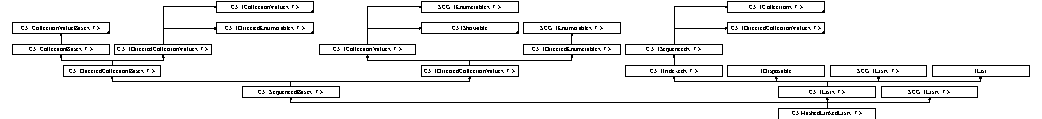
\includegraphics[height=1.577465cm]{class_c5_1_1_hashed_linked_list}
\end{center}
\end{figure}
\subsection*{Public Member Functions}
\begin{DoxyCompactItemize}
\item 
\hyperlink{class_c5_1_1_hashed_linked_list_a2adc87edb033f3ffef4b3b8e0b7ee647}{Hashed\+Linked\+List} (S\+C\+G.\+I\+Equality\+Comparer$<$ T $>$ \hyperlink{class_c5_1_1_collection_base_a95e343400be0e8f3f8d6310f1aaf2cc6}{itemequality\+Comparer})
\begin{DoxyCompactList}\small\item\em Create a linked list with en external item equality\+Comparer \end{DoxyCompactList}\item 
\hyperlink{class_c5_1_1_hashed_linked_list_a84e3034fe412b1ac30c2d06db071dc1d}{Hashed\+Linked\+List} ()
\begin{DoxyCompactList}\small\item\em Create a linked list with the natural item equality\+Comparer \end{DoxyCompactList}\item 
virtual void \hyperlink{class_c5_1_1_hashed_linked_list_aef617151cd77e8458a49ef537dc5f8f8}{Dispose} ()
\begin{DoxyCompactList}\small\item\em Invalidate this list. If a view, just invalidate the view. If not a view, invalidate the list and all views on it. \end{DoxyCompactList}\item 
virtual void \hyperlink{class_c5_1_1_hashed_linked_list_a7aef654591ab7641836af2f7fb29c9cc}{Insert} (int i, T item)
\begin{DoxyCompactList}\small\item\em Insert an item at a specific index location in this list. 
\begin{DoxyExceptions}{Exceptions}
{\em Index\+Out\+Of\+Range\+Exception} & if i is negative or $>$ the size of the collection.\\
\hline
\end{DoxyExceptions}
\end{DoxyCompactList}\item 
void \hyperlink{class_c5_1_1_hashed_linked_list_a3ad04f5ddf6a1a8dd8ca517f7298aee0}{Insert} (\hyperlink{interface_c5_1_1_i_list}{I\+List}$<$ T $>$ pointer, T item)
\begin{DoxyCompactList}\small\item\em Insert an item at the end of a compatible view, used as a pointer. \end{DoxyCompactList}\item 
virtual void \hyperlink{class_c5_1_1_hashed_linked_list_a6e309a1f1e92f363e9a49695cb3e5ce2}{Insert\+All} (int i, S\+C\+G.\+I\+Enumerable$<$ T $>$ items)
\begin{DoxyCompactList}\small\item\em Insert into this list all items from an enumerable collection starting at a particular index. 
\begin{DoxyExceptions}{Exceptions}
{\em Index\+Out\+Of\+Range\+Exception} & if i is negative or $>$ the size of the collection. \\
\hline
\end{DoxyExceptions}
\end{DoxyCompactList}\item 
virtual void \hyperlink{class_c5_1_1_hashed_linked_list_ae02598bb941fbd2665b3b05c317aeadb}{Insert\+First} (T item)
\begin{DoxyCompactList}\small\item\em Insert an item at the front of this list. \end{DoxyCompactList}\item 
virtual void \hyperlink{class_c5_1_1_hashed_linked_list_a315e3df7f01e031e71d2da0581ee2598}{Insert\+Last} (T item)
\begin{DoxyCompactList}\small\item\em Insert an item at the back of this list. \end{DoxyCompactList}\item 
\hyperlink{interface_c5_1_1_i_list}{I\+List}$<$ V $>$ \hyperlink{class_c5_1_1_hashed_linked_list_adc35379b5a56bbaf7790dd26bcc8ab6b}{Map$<$ V $>$} (Func$<$ T, V $>$ mapper)
\begin{DoxyCompactList}\small\item\em Create a new list consisting of the results of mapping all items of this list. \end{DoxyCompactList}\item 
\hyperlink{interface_c5_1_1_i_list}{I\+List}$<$ V $>$ \hyperlink{class_c5_1_1_hashed_linked_list_a5785aad402110c74b1d100ba504d1d90}{Map$<$ V $>$} (Func$<$ T, V $>$ mapper, S\+C\+G.\+I\+Equality\+Comparer$<$ V $>$ equality\+Comparer)
\begin{DoxyCompactList}\small\item\em Create a new list consisting of the results of mapping all items of this list. The new list will use a specified equality\+Comparer for the item type. \end{DoxyCompactList}\item 
virtual T \hyperlink{class_c5_1_1_hashed_linked_list_a899849bf8ad50e60206c8b3b59611eaf}{Remove} ()
\begin{DoxyCompactList}\small\item\em Remove one item from the list\+: from the front if \end{DoxyCompactList}\item 
virtual T \hyperlink{class_c5_1_1_hashed_linked_list_ab319b375d54035e9599a018ea4c6f342}{Remove\+First} ()
\begin{DoxyCompactList}\small\item\em Remove one item from the front of the list. 
\begin{DoxyExceptions}{Exceptions}
{\em \hyperlink{class_c5_1_1_no_such_item_exception}{No\+Such\+Item\+Exception}} & if this list is empty. \\
\hline
\end{DoxyExceptions}
\end{DoxyCompactList}\item 
virtual T \hyperlink{class_c5_1_1_hashed_linked_list_a0fc592e8e1c3667b8e65f3b32eafe863}{Remove\+Last} ()
\begin{DoxyCompactList}\small\item\em Remove one item from the back of the list. 
\begin{DoxyExceptions}{Exceptions}
{\em \hyperlink{class_c5_1_1_no_such_item_exception}{No\+Such\+Item\+Exception}} & if this list is empty. \\
\hline
\end{DoxyExceptions}
\end{DoxyCompactList}\item 
virtual \hyperlink{interface_c5_1_1_i_list}{I\+List}$<$ T $>$ \hyperlink{class_c5_1_1_hashed_linked_list_a3a8fd36d2556ffdec212c2b5ab5dc8ab}{View} (int start, int count)
\begin{DoxyCompactList}\small\item\em Create a list view on this list. \end{DoxyCompactList}\item 
virtual \hyperlink{interface_c5_1_1_i_list}{I\+List}$<$ T $>$ \hyperlink{class_c5_1_1_hashed_linked_list_a7ef47c4c75f39782f7f846dadf892f20}{View\+Of} (T item)
\begin{DoxyCompactList}\small\item\em Create a list view on this list containing the (first) occurrence of a particular item. \end{DoxyCompactList}\item 
virtual \hyperlink{interface_c5_1_1_i_list}{I\+List}$<$ T $>$ \hyperlink{class_c5_1_1_hashed_linked_list_a3c61023f5a2ea2c6011b35dff34f4058}{Last\+View\+Of} (T item)
\begin{DoxyCompactList}\small\item\em Create a list view on this list containing the last occurrence of a particular item. 
\begin{DoxyExceptions}{Exceptions}
{\em Argument\+Exception} & if the item is not in this list. \\
\hline
\end{DoxyExceptions}
\end{DoxyCompactList}\item 
\hyperlink{interface_c5_1_1_i_list}{I\+List}$<$ T $>$ \hyperlink{class_c5_1_1_hashed_linked_list_ac53f2d792ff731a9e088c64c6c83a20c}{Slide} (int offset)
\begin{DoxyCompactList}\small\item\em Slide this list view along the underlying list. \end{DoxyCompactList}\item 
\hyperlink{interface_c5_1_1_i_list}{I\+List}$<$ T $>$ \hyperlink{class_c5_1_1_hashed_linked_list_acc3a108d2be072d5f3e83e96c80ff3c6}{Slide} (int offset, int \hyperlink{class_c5_1_1_collection_base_ab524b118754a5a8290b6528511272833}{size})
\begin{DoxyCompactList}\small\item\em Slide this list view along the underlying list, perhaps changing its size. \end{DoxyCompactList}\item 
virtual bool \hyperlink{class_c5_1_1_hashed_linked_list_a5b6ca6ab869f08c519ed94b8b5187eb9}{Try\+Slide} (int offset)
\item 
virtual bool \hyperlink{class_c5_1_1_hashed_linked_list_a8be27e432be4b0707f55c469794afec2}{Try\+Slide} (int offset, int \hyperlink{class_c5_1_1_collection_base_ab524b118754a5a8290b6528511272833}{size})
\item 
virtual \hyperlink{interface_c5_1_1_i_list}{I\+List}$<$ T $>$ \hyperlink{class_c5_1_1_hashed_linked_list_a50badd5da340247829b46327285e5d46}{Span} (\hyperlink{interface_c5_1_1_i_list}{I\+List}$<$ T $>$ other\+View)
\item 
virtual void \hyperlink{class_c5_1_1_hashed_linked_list_a1390f0566000923c714fe19d1d2792d3}{Reverse} ()
\begin{DoxyCompactList}\small\item\em Reverse the list so the items are in the opposite sequence order. \end{DoxyCompactList}\item 
bool \hyperlink{class_c5_1_1_hashed_linked_list_ab34c0de0335ccd7d9d16efd159d4411b}{Is\+Sorted} ()
\begin{DoxyCompactList}\small\item\em Check if this list is sorted according to the default sorting order for the item type T, as defined by the T\+:\+C5.\+Comparer`1 class \end{DoxyCompactList}\item 
virtual bool \hyperlink{class_c5_1_1_hashed_linked_list_a7d539fd8712f39feca8e3b1c561e8850}{Is\+Sorted} (S\+C\+G.\+I\+Comparer$<$ T $>$ c)
\begin{DoxyCompactList}\small\item\em Check if this list is sorted according to a specific sorting order. \end{DoxyCompactList}\item 
virtual void \hyperlink{class_c5_1_1_hashed_linked_list_aec6a08f56ea7e0824118849c15f17b62}{Sort} ()
\begin{DoxyCompactList}\small\item\em Sort the items of the list according to the default sorting order for the item type T, as defined by the Comparer\mbox{[}T\mbox{]} class. (T\+:\+C5.\+Comparer`1). The sorting is stable. \end{DoxyCompactList}\item 
virtual void \hyperlink{class_c5_1_1_hashed_linked_list_a017110699d25ae50b4ea7687c71e64a4}{Sort} (S\+C\+G.\+I\+Comparer$<$ T $>$ c)
\begin{DoxyCompactList}\small\item\em Sort the items of the list according to a specific sorting order. The sorting is stable. \end{DoxyCompactList}\item 
virtual void \hyperlink{class_c5_1_1_hashed_linked_list_a7d705d1d949be5d4b6a154d2c9f28200}{Shuffle} ()
\begin{DoxyCompactList}\small\item\em Randomly shuffle the items of this list. \end{DoxyCompactList}\item 
virtual void \hyperlink{class_c5_1_1_hashed_linked_list_acb52fe8c7bce2ed047c03b3718eab410}{Shuffle} (Random rnd)
\begin{DoxyCompactList}\small\item\em Shuffle the items of this list according to a specific random source. \end{DoxyCompactList}\item 
virtual int \hyperlink{class_c5_1_1_hashed_linked_list_aca8634364d0bfec4b0d2bb8b7c6f5c98}{Index\+Of} (T item)
\begin{DoxyCompactList}\small\item\em Searches for an item in the list going forwrds from the start. \end{DoxyCompactList}\item 
virtual int \hyperlink{class_c5_1_1_hashed_linked_list_a4e053c03fa87e356bab7ec25a529607a}{Last\+Index\+Of} (T item)
\begin{DoxyCompactList}\small\item\em Searches for an item in the list going backwords from the end. \end{DoxyCompactList}\item 
virtual T \hyperlink{class_c5_1_1_hashed_linked_list_ae29691247778dcae44ae4a4482c4c94f}{Remove\+At} (int i)
\begin{DoxyCompactList}\small\item\em Remove the item at a specific position of the list. 
\begin{DoxyExceptions}{Exceptions}
{\em Index\+Out\+Of\+Range\+Exception} & if i is negative or $>$= the size of the collection. \\
\hline
\end{DoxyExceptions}
\end{DoxyCompactList}\item 
virtual void \hyperlink{class_c5_1_1_hashed_linked_list_ab2b43feeeb2c5cece0d5e65949c178b3}{Remove\+Interval} (int start, int count)
\begin{DoxyCompactList}\small\item\em Remove all items in an index interval. 
\begin{DoxyExceptions}{Exceptions}
{\em Index\+Out\+Of\+Range\+Exception} & ???. \\
\hline
\end{DoxyExceptions}
\end{DoxyCompactList}\item 
override int \hyperlink{class_c5_1_1_hashed_linked_list_ab1ef52935e3a9a7ba78b1ddecc7a696e}{Get\+Sequenced\+Hash\+Code} ()
\item 
override bool \hyperlink{class_c5_1_1_hashed_linked_list_a473d18abd8b89ee61184fd6731e76029}{Sequenced\+Equals} (\hyperlink{interface_c5_1_1_i_sequenced}{I\+Sequenced}$<$ T $>$ that)
\item 
override \hyperlink{interface_c5_1_1_i_directed_collection_value}{I\+Directed\+Collection\+Value}$<$ T $>$ \hyperlink{class_c5_1_1_hashed_linked_list_ad0fbbf15338c5aae4278a5e44f8d9c69}{Backwards} ()
\begin{DoxyCompactList}\small\item\em Create a collection containing the same items as this collection, but whose enumerator will enumerate the items backwards. The new collection will become invalid if the original is modified. Method typicaly used as in \end{DoxyCompactList}\item 
override int \hyperlink{class_c5_1_1_hashed_linked_list_afa9c20b419017663841ffd613d31e75b}{Get\+Unsequenced\+Hash\+Code} ()
\begin{DoxyCompactList}\small\item\em Performs a check for view validity before calling base.\+Get\+Unsequenced\+Hash\+Code() \end{DoxyCompactList}\item 
override bool \hyperlink{class_c5_1_1_hashed_linked_list_a658a0145c6f1d28e00e558a705d3c8e2}{Unsequenced\+Equals} (\hyperlink{interface_c5_1_1_i_collection}{I\+Collection}$<$ T $>$ that)
\item 
virtual bool \hyperlink{class_c5_1_1_hashed_linked_list_a210cb416cd7418c59c89b99e2fce7bf8}{Contains} (T item)
\begin{DoxyCompactList}\small\item\em Check if this collection contains (an item equivalent to according to the itemequality\+Comparer) a particular value. \end{DoxyCompactList}\item 
virtual bool \hyperlink{class_c5_1_1_hashed_linked_list_a71b0404288670bcd57700dafe8f9933c}{Find} (ref T item)
\begin{DoxyCompactList}\small\item\em Check if this collection contains an item equivalent according to the itemequality\+Comparer to a particular value. If so, return in the ref argument (a binary copy of) the actual value found. \end{DoxyCompactList}\item 
virtual bool \hyperlink{class_c5_1_1_hashed_linked_list_a1c0b09fb0b46cc0bcc00e67e5d027438}{Update} (T item)
\begin{DoxyCompactList}\small\item\em Check if this collection contains an item equivalent according to the itemequality\+Comparer to a particular value. If so, update the item in the collection to with a binary copy of the supplied value. Will update a single item. \end{DoxyCompactList}\item 
virtual bool \hyperlink{class_c5_1_1_hashed_linked_list_a67ca2384da1dde0b651fe1ec01c8f0ba}{Update} (T item, out T olditem)
\item 
virtual bool \hyperlink{class_c5_1_1_hashed_linked_list_a71a1257a1ba4328713fb87daa3b45675}{Find\+Or\+Add} (ref T item)
\begin{DoxyCompactList}\small\item\em Check if this collection contains an item equivalent according to the itemequality\+Comparer to a particular value. If so, return in the ref argument (a binary copy of) the actual value found. Else, add the item to the collection. \end{DoxyCompactList}\item 
virtual bool \hyperlink{class_c5_1_1_hashed_linked_list_a5efb946b793ca1134c8f9d8b47d2cac7}{Update\+Or\+Add} (T item)
\begin{DoxyCompactList}\small\item\em Check if this collection contains an item equivalent according to the itemequality\+Comparer to a particular value. If so, update the item in the collection to with a binary copy of the supplied value; else add the value to the collection. \end{DoxyCompactList}\item 
virtual bool \hyperlink{class_c5_1_1_hashed_linked_list_a53e4be293af672a2354b7eb480ce48e6}{Update\+Or\+Add} (T item, out T olditem)
\item 
virtual bool \hyperlink{class_c5_1_1_hashed_linked_list_ad97f128fe00bf12c8e77678f08bd27e1}{Remove} (T item)
\begin{DoxyCompactList}\small\item\em Remove a particular item from this collection. Since the collection has bag semantics only one copy equivalent to the supplied item is removed. \end{DoxyCompactList}\item 
virtual bool \hyperlink{class_c5_1_1_hashed_linked_list_ab1348cf4b0e02e147f6dd08a539e2c61}{Remove} (T item, out T removeditem)
\begin{DoxyCompactList}\small\item\em Remove a particular item from this collection if found (only one copy). If an item was removed, report a binary copy of the actual item removed in the argument. \end{DoxyCompactList}\item 
virtual void \hyperlink{class_c5_1_1_hashed_linked_list_a13f0ec0b64eaba0412a48e8df37ba210}{Remove\+All} (S\+C\+G.\+I\+Enumerable$<$ T $>$ items)
\begin{DoxyCompactList}\small\item\em Remove all items in another collection from this one, taking multiplicities into account. \end{DoxyCompactList}\item 
virtual void \hyperlink{class_c5_1_1_hashed_linked_list_a3d890e2da8746df9cf82d3ccaf561d44}{Clear} ()
\begin{DoxyCompactList}\small\item\em Remove all items from this collection. \end{DoxyCompactList}\item 
virtual void \hyperlink{class_c5_1_1_hashed_linked_list_a56ae0d7eee62da4832bfc2363adf056e}{Retain\+All} (S\+C\+G.\+I\+Enumerable$<$ T $>$ items)
\begin{DoxyCompactList}\small\item\em Remove all items not in some other collection from this one, taking multiplicities into account. \end{DoxyCompactList}\item 
virtual bool \hyperlink{class_c5_1_1_hashed_linked_list_a8592fd2f2b3cea5329acaf4331dff7bc}{Contains\+All} (S\+C\+G.\+I\+Enumerable$<$ T $>$ items)
\begin{DoxyCompactList}\small\item\em Check if this collection contains all the values in another collection with respect to multiplicities. \end{DoxyCompactList}\item 
\hyperlink{interface_c5_1_1_i_list}{I\+List}$<$ T $>$ \hyperlink{class_c5_1_1_hashed_linked_list_a4a12ba4a72a0d544589a4aabba1c63de}{Find\+All} (Func$<$ T, bool $>$ filter)
\begin{DoxyCompactList}\small\item\em Create a new list consisting of the items of this list satisfying a certain predicate. \end{DoxyCompactList}\item 
virtual int \hyperlink{class_c5_1_1_hashed_linked_list_a0bf0f2c26ac2975f17d240880ca79de5}{Contains\+Count} (T item)
\begin{DoxyCompactList}\small\item\em Count the number of items of the collection equal to a particular value. Returns 0 if and only if the value is not in the collection. \end{DoxyCompactList}\item 
virtual \hyperlink{interface_c5_1_1_i_collection_value}{I\+Collection\+Value}$<$ T $>$ \hyperlink{class_c5_1_1_hashed_linked_list_a11f80f9fc36538f944da608ce8ae8e6e}{Unique\+Items} ()
\item 
virtual \hyperlink{interface_c5_1_1_i_collection_value}{I\+Collection\+Value}$<$ \hyperlink{struct_c5_1_1_key_value_pair}{Key\+Value\+Pair}$<$ T, int $>$ $>$ \hyperlink{class_c5_1_1_hashed_linked_list_a0cee8e4c1768986a4d167f34c8a3c227}{Item\+Multiplicities} ()
\item 
virtual void \hyperlink{class_c5_1_1_hashed_linked_list_ad3b535da6c6624412c450c96560d2f51}{Remove\+All\+Copies} (T item)
\begin{DoxyCompactList}\small\item\em Remove all items equivalent to a given value. \end{DoxyCompactList}\item 
override T \hyperlink{class_c5_1_1_hashed_linked_list_a8f4365d623d3424943b1891e998fc90d}{Choose} ()
\begin{DoxyCompactList}\small\item\em Choose some item of this collection. \end{DoxyCompactList}\item 
override S\+C\+G.\+I\+Enumerable$<$ T $>$ \hyperlink{class_c5_1_1_hashed_linked_list_ad092b0255821d358df6cfe045870e256}{Filter} (Func$<$ T, bool $>$ filter)
\begin{DoxyCompactList}\small\item\em Create an enumerable, enumerating the items of this collection that satisfies a certain condition. \end{DoxyCompactList}\item 
override S\+C\+G.\+I\+Enumerator$<$ T $>$ \hyperlink{class_c5_1_1_hashed_linked_list_ae8f40668f13afb6cb05501446a3bcc4e}{Get\+Enumerator} ()
\begin{DoxyCompactList}\small\item\em Create an enumerator for the collection \end{DoxyCompactList}\item 
virtual bool \hyperlink{class_c5_1_1_hashed_linked_list_afcfc7b8da2f00ad7d8e3decadadd74bc}{Add} (T item)
\begin{DoxyCompactList}\small\item\em Add an item to this collection if possible. \end{DoxyCompactList}\item 
virtual void \hyperlink{class_c5_1_1_hashed_linked_list_a546555b545da25f99c4ca0e1dc31ddab}{Add\+All} (S\+C\+G.\+I\+Enumerable$<$ T $>$ items)
\begin{DoxyCompactList}\small\item\em Add the elements from another collection with a more specialized item type to this collection. \end{DoxyCompactList}\item 
virtual bool \hyperlink{class_c5_1_1_hashed_linked_list_a03cc4fb3b1f5e3172df5ac12f72167b3}{Check} ()
\begin{DoxyCompactList}\small\item\em Check the sanity of this list \end{DoxyCompactList}\end{DoxyCompactItemize}
\subsection*{Protected Member Functions}
\begin{DoxyCompactItemize}
\item 
override void \hyperlink{class_c5_1_1_hashed_linked_list_af71c07992c8c580b5624734cbdd1bd4e}{updatecheck} ()
\begin{DoxyCompactList}\small\item\em Check if it is valid to perform updates and increment stamp of underlying if this is a view. \end{DoxyCompactList}\item 
override void \hyperlink{class_c5_1_1_hashed_linked_list_a1e067df13f4f6b5f90753abf3db99ed7}{modifycheck} (int \hyperlink{class_c5_1_1_collection_base_ae13bd5b482306a49a4d10654a9b8b064}{stamp})
\begin{DoxyCompactList}\small\item\em Check that the list has not been updated since a particular time. \end{DoxyCompactList}\end{DoxyCompactItemize}
\subsection*{Properties}
\begin{DoxyCompactItemize}
\item 
override \hyperlink{namespace_c5_a9143bfd561fffa025d21561674758008}{Event\+Type\+Enum} \hyperlink{class_c5_1_1_hashed_linked_list_a2eab2146c49daf255c542b957656b25c}{Listenable\+Events}\hspace{0.3cm}{\ttfamily  \mbox{[}get\mbox{]}}
\item 
virtual T \hyperlink{class_c5_1_1_hashed_linked_list_a364ea12660521152709ecb6ea0ff231d}{First}\hspace{0.3cm}{\ttfamily  \mbox{[}get\mbox{]}}
\item 
virtual T \hyperlink{class_c5_1_1_hashed_linked_list_ab47e317103cce4499a55bac8b1aac351}{Last}\hspace{0.3cm}{\ttfamily  \mbox{[}get\mbox{]}}
\item 
virtual bool \hyperlink{class_c5_1_1_hashed_linked_list_a177c8639ed7154131ac278bac877fd0c}{F\+I\+F\+O}\hspace{0.3cm}{\ttfamily  \mbox{[}get, set\mbox{]}}
\begin{DoxyCompactList}\small\item\em Since \end{DoxyCompactList}\item 
virtual bool \hyperlink{class_c5_1_1_hashed_linked_list_ae5328883cfc6d4f3415635f4fd2fb0fc}{Is\+Fixed\+Size}\hspace{0.3cm}{\ttfamily  \mbox{[}get\mbox{]}}
\item 
virtual T \hyperlink{class_c5_1_1_hashed_linked_list_aacd03b9a2e43ade0185cf745b3374994}{this\mbox{[}int index\mbox{]}}\hspace{0.3cm}{\ttfamily  \mbox{[}get, set\mbox{]}}
\begin{DoxyCompactList}\small\item\em On this list, this indexer is read/write. 
\begin{DoxyExceptions}{Exceptions}
{\em Index\+Out\+Of\+Range\+Exception} & if i is negative or $>$= the size of the collection. \\
\hline
\end{DoxyExceptions}
\end{DoxyCompactList}\item 
virtual \hyperlink{namespace_c5_a615ba88dcdaa8d5a3c5f833a73d7fad6}{Speed} \hyperlink{class_c5_1_1_hashed_linked_list_aa72a5381efc4af4311dabc4b1b214ec4}{Indexing\+Speed}\hspace{0.3cm}{\ttfamily  \mbox{[}get\mbox{]}}
\item 
virtual \hyperlink{interface_c5_1_1_i_list}{I\+List}$<$ T $>$ \hyperlink{class_c5_1_1_hashed_linked_list_ab70556e117c40bfeea64e24daa937955}{Underlying}\hspace{0.3cm}{\ttfamily  \mbox{[}get\mbox{]}}
\begin{DoxyCompactList}\small\item\em Null if this list is not a view. \end{DoxyCompactList}\item 
virtual bool \hyperlink{class_c5_1_1_hashed_linked_list_a548a9179889fa5600ad6cea96b341893}{Is\+Valid}\hspace{0.3cm}{\ttfamily  \mbox{[}get\mbox{]}}
\item 
virtual int \hyperlink{class_c5_1_1_hashed_linked_list_aae6da46ea57defcd779416e00622adbb}{Offset}\hspace{0.3cm}{\ttfamily  \mbox{[}get\mbox{]}}
\item 
\hyperlink{interface_c5_1_1_i_directed_collection_value}{I\+Directed\+Collection\+Value}$<$ T $>$ \hyperlink{class_c5_1_1_hashed_linked_list_aaf5b40fcd1eaa99ad9d4a0127f286e3f}{this\mbox{[}int start, int count\mbox{]}}\hspace{0.3cm}{\ttfamily  \mbox{[}get\mbox{]}}
\begin{DoxyCompactList}\small\item\em 
\begin{DoxyExceptions}{Exceptions}
{\em Index\+Out\+Of\+Range\+Exception} & . \\
\hline
\end{DoxyExceptions}
\end{DoxyCompactList}\item 
virtual \hyperlink{namespace_c5_a615ba88dcdaa8d5a3c5f833a73d7fad6}{Speed} \hyperlink{class_c5_1_1_hashed_linked_list_adfd49be207b1d5fe11d101a27ce194f1}{Contains\+Speed}\hspace{0.3cm}{\ttfamily  \mbox{[}get\mbox{]}}
\begin{DoxyCompactList}\small\item\em The value is symbolic indicating the type of asymptotic complexity in terms of the size of this collection (worst-\/case or amortized as relevant). \end{DoxyCompactList}\item 
override int \hyperlink{class_c5_1_1_hashed_linked_list_a73efb105a40772ad5ca242801db6d5ff}{Count}\hspace{0.3cm}{\ttfamily  \mbox{[}get\mbox{]}}
\item 
virtual bool \hyperlink{class_c5_1_1_hashed_linked_list_a0a771fb597422ba1c79972188d9102fa}{Allows\+Duplicates}\hspace{0.3cm}{\ttfamily  \mbox{[}get\mbox{]}}
\item 
virtual bool \hyperlink{class_c5_1_1_hashed_linked_list_a3106d441e4ac4a901b7f464402957382}{Duplicates\+By\+Counting}\hspace{0.3cm}{\ttfamily  \mbox{[}get\mbox{]}}
\begin{DoxyCompactList}\small\item\em By convention this is true for any collection with set semantics. \end{DoxyCompactList}\end{DoxyCompactItemize}
\subsection*{Additional Inherited Members}


\subsection{Detailed Description}
A list collection class based on a doubly linked list data structure. 



\subsection{Constructor \& Destructor Documentation}
\hypertarget{class_c5_1_1_hashed_linked_list_a2adc87edb033f3ffef4b3b8e0b7ee647}{}\index{C5\+::\+Hashed\+Linked\+List@{C5\+::\+Hashed\+Linked\+List}!Hashed\+Linked\+List@{Hashed\+Linked\+List}}
\index{Hashed\+Linked\+List@{Hashed\+Linked\+List}!C5\+::\+Hashed\+Linked\+List@{C5\+::\+Hashed\+Linked\+List}}
\subsubsection[{Hashed\+Linked\+List(\+S\+C\+G.\+I\+Equality\+Comparer$<$ T $>$ itemequality\+Comparer)}]{\setlength{\rightskip}{0pt plus 5cm}{\bf C5.\+Hashed\+Linked\+List}$<$ T $>$.{\bf Hashed\+Linked\+List} (
\begin{DoxyParamCaption}
\item[{S\+C\+G.\+I\+Equality\+Comparer$<$ T $>$}]{itemequality\+Comparer}
\end{DoxyParamCaption}
)}\label{class_c5_1_1_hashed_linked_list_a2adc87edb033f3ffef4b3b8e0b7ee647}


Create a linked list with en external item equality\+Comparer 


\begin{DoxyParams}{Parameters}
{\em itemequality\+Comparer} & The external equality\+S\+C\+G.\+Comparer\\
\hline
\end{DoxyParams}
\hypertarget{class_c5_1_1_hashed_linked_list_a84e3034fe412b1ac30c2d06db071dc1d}{}\index{C5\+::\+Hashed\+Linked\+List@{C5\+::\+Hashed\+Linked\+List}!Hashed\+Linked\+List@{Hashed\+Linked\+List}}
\index{Hashed\+Linked\+List@{Hashed\+Linked\+List}!C5\+::\+Hashed\+Linked\+List@{C5\+::\+Hashed\+Linked\+List}}
\subsubsection[{Hashed\+Linked\+List()}]{\setlength{\rightskip}{0pt plus 5cm}{\bf C5.\+Hashed\+Linked\+List}$<$ T $>$.{\bf Hashed\+Linked\+List} (
\begin{DoxyParamCaption}
{}
\end{DoxyParamCaption}
)}\label{class_c5_1_1_hashed_linked_list_a84e3034fe412b1ac30c2d06db071dc1d}


Create a linked list with the natural item equality\+Comparer 



\subsection{Member Function Documentation}
\hypertarget{class_c5_1_1_hashed_linked_list_afcfc7b8da2f00ad7d8e3decadadd74bc}{}\index{C5\+::\+Hashed\+Linked\+List@{C5\+::\+Hashed\+Linked\+List}!Add@{Add}}
\index{Add@{Add}!C5\+::\+Hashed\+Linked\+List@{C5\+::\+Hashed\+Linked\+List}}
\subsubsection[{Add(\+T item)}]{\setlength{\rightskip}{0pt plus 5cm}virtual bool {\bf C5.\+Hashed\+Linked\+List}$<$ T $>$.Add (
\begin{DoxyParamCaption}
\item[{T}]{item}
\end{DoxyParamCaption}
)\hspace{0.3cm}{\ttfamily [virtual]}}\label{class_c5_1_1_hashed_linked_list_afcfc7b8da2f00ad7d8e3decadadd74bc}


Add an item to this collection if possible. 


\begin{DoxyParams}{Parameters}
{\em item} & The item to add.\\
\hline
\end{DoxyParams}
\begin{DoxyReturn}{Returns}
True.
\end{DoxyReturn}


Implements \hyperlink{interface_c5_1_1_i_list_a800000d7344d000c1b8c67acda464a3d}{C5.\+I\+List$<$ T $>$}.

\hypertarget{class_c5_1_1_hashed_linked_list_a546555b545da25f99c4ca0e1dc31ddab}{}\index{C5\+::\+Hashed\+Linked\+List@{C5\+::\+Hashed\+Linked\+List}!Add\+All@{Add\+All}}
\index{Add\+All@{Add\+All}!C5\+::\+Hashed\+Linked\+List@{C5\+::\+Hashed\+Linked\+List}}
\subsubsection[{Add\+All(\+S\+C\+G.\+I\+Enumerable$<$ T $>$ items)}]{\setlength{\rightskip}{0pt plus 5cm}virtual void {\bf C5.\+Hashed\+Linked\+List}$<$ T $>$.Add\+All (
\begin{DoxyParamCaption}
\item[{S\+C\+G.\+I\+Enumerable$<$ T $>$}]{items}
\end{DoxyParamCaption}
)\hspace{0.3cm}{\ttfamily [virtual]}}\label{class_c5_1_1_hashed_linked_list_a546555b545da25f99c4ca0e1dc31ddab}


Add the elements from another collection with a more specialized item type to this collection. 


\begin{DoxyParams}{Parameters}
{\em items} & The items to add\\
\hline
\end{DoxyParams}


Implements \hyperlink{interface_c5_1_1_i_extensible_a1fb4d50c5b340e60303da72e9d0ede6e}{C5.\+I\+Extensible$<$ T $>$}.

\hypertarget{class_c5_1_1_hashed_linked_list_ad0fbbf15338c5aae4278a5e44f8d9c69}{}\index{C5\+::\+Hashed\+Linked\+List@{C5\+::\+Hashed\+Linked\+List}!Backwards@{Backwards}}
\index{Backwards@{Backwards}!C5\+::\+Hashed\+Linked\+List@{C5\+::\+Hashed\+Linked\+List}}
\subsubsection[{Backwards()}]{\setlength{\rightskip}{0pt plus 5cm}override {\bf I\+Directed\+Collection\+Value}$<$T$>$ {\bf C5.\+Hashed\+Linked\+List}$<$ T $>$.Backwards (
\begin{DoxyParamCaption}
{}
\end{DoxyParamCaption}
)\hspace{0.3cm}{\ttfamily [virtual]}}\label{class_c5_1_1_hashed_linked_list_ad0fbbf15338c5aae4278a5e44f8d9c69}


Create a collection containing the same items as this collection, but whose enumerator will enumerate the items backwards. The new collection will become invalid if the original is modified. Method typicaly used as in 

{\ttfamily foreach (T x in \hyperlink{namespace_c5_aad282676794e49130eb8caed289395f8a9d1104e419414f4c268be7211fb8fc4a}{coll.\+Backwards()}) \{...\}} 

\begin{DoxyReturn}{Returns}
The backwards collection.
\end{DoxyReturn}


Implements \hyperlink{class_c5_1_1_directed_collection_base_a9a4c7d6571ff7d78ea5adcb0d8264ff1}{C5.\+Directed\+Collection\+Base$<$ T $>$}.

\hypertarget{class_c5_1_1_hashed_linked_list_a03cc4fb3b1f5e3172df5ac12f72167b3}{}\index{C5\+::\+Hashed\+Linked\+List@{C5\+::\+Hashed\+Linked\+List}!Check@{Check}}
\index{Check@{Check}!C5\+::\+Hashed\+Linked\+List@{C5\+::\+Hashed\+Linked\+List}}
\subsubsection[{Check()}]{\setlength{\rightskip}{0pt plus 5cm}virtual bool {\bf C5.\+Hashed\+Linked\+List}$<$ T $>$.Check (
\begin{DoxyParamCaption}
{}
\end{DoxyParamCaption}
)\hspace{0.3cm}{\ttfamily [virtual]}}\label{class_c5_1_1_hashed_linked_list_a03cc4fb3b1f5e3172df5ac12f72167b3}


Check the sanity of this list 

\begin{DoxyReturn}{Returns}
true if sane
\end{DoxyReturn}


Implements \hyperlink{interface_c5_1_1_i_extensible_aeeb6b87af61e455df42d68834d711bcb}{C5.\+I\+Extensible$<$ T $>$}.

\hypertarget{class_c5_1_1_hashed_linked_list_a8f4365d623d3424943b1891e998fc90d}{}\index{C5\+::\+Hashed\+Linked\+List@{C5\+::\+Hashed\+Linked\+List}!Choose@{Choose}}
\index{Choose@{Choose}!C5\+::\+Hashed\+Linked\+List@{C5\+::\+Hashed\+Linked\+List}}
\subsubsection[{Choose()}]{\setlength{\rightskip}{0pt plus 5cm}override T {\bf C5.\+Hashed\+Linked\+List}$<$ T $>$.Choose (
\begin{DoxyParamCaption}
{}
\end{DoxyParamCaption}
)}\label{class_c5_1_1_hashed_linked_list_a8f4365d623d3424943b1891e998fc90d}


Choose some item of this collection. 


\begin{DoxyExceptions}{Exceptions}
{\em \hyperlink{class_c5_1_1_no_such_item_exception}{No\+Such\+Item\+Exception}} & if collection is empty.\\
\hline
\end{DoxyExceptions}
\begin{DoxyReturn}{Returns}

\end{DoxyReturn}


Implements \hyperlink{interface_c5_1_1_i_collection_value_af72d52ddd8ea4130d508e1cf020cf7eb}{C5.\+I\+Collection\+Value$<$ T $>$}.

\hypertarget{class_c5_1_1_hashed_linked_list_a3d890e2da8746df9cf82d3ccaf561d44}{}\index{C5\+::\+Hashed\+Linked\+List@{C5\+::\+Hashed\+Linked\+List}!Clear@{Clear}}
\index{Clear@{Clear}!C5\+::\+Hashed\+Linked\+List@{C5\+::\+Hashed\+Linked\+List}}
\subsubsection[{Clear()}]{\setlength{\rightskip}{0pt plus 5cm}virtual void {\bf C5.\+Hashed\+Linked\+List}$<$ T $>$.Clear (
\begin{DoxyParamCaption}
{}
\end{DoxyParamCaption}
)\hspace{0.3cm}{\ttfamily [virtual]}}\label{class_c5_1_1_hashed_linked_list_a3d890e2da8746df9cf82d3ccaf561d44}


Remove all items from this collection. 



Implements \hyperlink{interface_c5_1_1_i_list_aff6179e37b313d34596749484ae58ea4}{C5.\+I\+List$<$ T $>$}.

\hypertarget{class_c5_1_1_hashed_linked_list_a210cb416cd7418c59c89b99e2fce7bf8}{}\index{C5\+::\+Hashed\+Linked\+List@{C5\+::\+Hashed\+Linked\+List}!Contains@{Contains}}
\index{Contains@{Contains}!C5\+::\+Hashed\+Linked\+List@{C5\+::\+Hashed\+Linked\+List}}
\subsubsection[{Contains(\+T item)}]{\setlength{\rightskip}{0pt plus 5cm}virtual bool {\bf C5.\+Hashed\+Linked\+List}$<$ T $>$.Contains (
\begin{DoxyParamCaption}
\item[{T}]{item}
\end{DoxyParamCaption}
)\hspace{0.3cm}{\ttfamily [virtual]}}\label{class_c5_1_1_hashed_linked_list_a210cb416cd7418c59c89b99e2fce7bf8}


Check if this collection contains (an item equivalent to according to the itemequality\+Comparer) a particular value. 


\begin{DoxyParams}{Parameters}
{\em item} & The value to check for.\\
\hline
\end{DoxyParams}
\begin{DoxyReturn}{Returns}
True if the items is in this collection.
\end{DoxyReturn}


Implements \hyperlink{interface_c5_1_1_i_list_a108b607b042959d063e1ca77e242406c}{C5.\+I\+List$<$ T $>$}.

\hypertarget{class_c5_1_1_hashed_linked_list_a8592fd2f2b3cea5329acaf4331dff7bc}{}\index{C5\+::\+Hashed\+Linked\+List@{C5\+::\+Hashed\+Linked\+List}!Contains\+All@{Contains\+All}}
\index{Contains\+All@{Contains\+All}!C5\+::\+Hashed\+Linked\+List@{C5\+::\+Hashed\+Linked\+List}}
\subsubsection[{Contains\+All(\+S\+C\+G.\+I\+Enumerable$<$ T $>$ items)}]{\setlength{\rightskip}{0pt plus 5cm}virtual bool {\bf C5.\+Hashed\+Linked\+List}$<$ T $>$.Contains\+All (
\begin{DoxyParamCaption}
\item[{S\+C\+G.\+I\+Enumerable$<$ T $>$}]{items}
\end{DoxyParamCaption}
)\hspace{0.3cm}{\ttfamily [virtual]}}\label{class_c5_1_1_hashed_linked_list_a8592fd2f2b3cea5329acaf4331dff7bc}


Check if this collection contains all the values in another collection with respect to multiplicities. 


\begin{DoxyParams}{Parameters}
{\em items} & The \\
\hline
\end{DoxyParams}
\begin{DoxyReturn}{Returns}
True if all values in 
\begin{DoxyCode}
items
\end{DoxyCode}
is in this collection.
\end{DoxyReturn}


Implements \hyperlink{interface_c5_1_1_i_collection_a93abf02183a46f56af8d90f1d69982a8}{C5.\+I\+Collection$<$ T $>$}.

\hypertarget{class_c5_1_1_hashed_linked_list_a0bf0f2c26ac2975f17d240880ca79de5}{}\index{C5\+::\+Hashed\+Linked\+List@{C5\+::\+Hashed\+Linked\+List}!Contains\+Count@{Contains\+Count}}
\index{Contains\+Count@{Contains\+Count}!C5\+::\+Hashed\+Linked\+List@{C5\+::\+Hashed\+Linked\+List}}
\subsubsection[{Contains\+Count(\+T item)}]{\setlength{\rightskip}{0pt plus 5cm}virtual int {\bf C5.\+Hashed\+Linked\+List}$<$ T $>$.Contains\+Count (
\begin{DoxyParamCaption}
\item[{T}]{item}
\end{DoxyParamCaption}
)\hspace{0.3cm}{\ttfamily [virtual]}}\label{class_c5_1_1_hashed_linked_list_a0bf0f2c26ac2975f17d240880ca79de5}


Count the number of items of the collection equal to a particular value. Returns 0 if and only if the value is not in the collection. 


\begin{DoxyParams}{Parameters}
{\em item} & The value to count.\\
\hline
\end{DoxyParams}
\begin{DoxyReturn}{Returns}
The number of copies found.
\end{DoxyReturn}


Implements \hyperlink{interface_c5_1_1_i_collection_acfe7e2c9b14c384762269edbb57b7fbe}{C5.\+I\+Collection$<$ T $>$}.

\hypertarget{class_c5_1_1_hashed_linked_list_aef617151cd77e8458a49ef537dc5f8f8}{}\index{C5\+::\+Hashed\+Linked\+List@{C5\+::\+Hashed\+Linked\+List}!Dispose@{Dispose}}
\index{Dispose@{Dispose}!C5\+::\+Hashed\+Linked\+List@{C5\+::\+Hashed\+Linked\+List}}
\subsubsection[{Dispose()}]{\setlength{\rightskip}{0pt plus 5cm}virtual void {\bf C5.\+Hashed\+Linked\+List}$<$ T $>$.Dispose (
\begin{DoxyParamCaption}
{}
\end{DoxyParamCaption}
)\hspace{0.3cm}{\ttfamily [virtual]}}\label{class_c5_1_1_hashed_linked_list_aef617151cd77e8458a49ef537dc5f8f8}


Invalidate this list. If a view, just invalidate the view. If not a view, invalidate the list and all views on it. 

\hypertarget{class_c5_1_1_hashed_linked_list_ad092b0255821d358df6cfe045870e256}{}\index{C5\+::\+Hashed\+Linked\+List@{C5\+::\+Hashed\+Linked\+List}!Filter@{Filter}}
\index{Filter@{Filter}!C5\+::\+Hashed\+Linked\+List@{C5\+::\+Hashed\+Linked\+List}}
\subsubsection[{Filter(\+Func$<$ T, bool $>$ filter)}]{\setlength{\rightskip}{0pt plus 5cm}override S\+C\+G.\+I\+Enumerable$<$T$>$ {\bf C5.\+Hashed\+Linked\+List}$<$ T $>$.Filter (
\begin{DoxyParamCaption}
\item[{Func$<$ T, bool $>$}]{filter}
\end{DoxyParamCaption}
)}\label{class_c5_1_1_hashed_linked_list_ad092b0255821d358df6cfe045870e256}


Create an enumerable, enumerating the items of this collection that satisfies a certain condition. 


\begin{DoxyParams}{Parameters}
{\em filter} & The T-\/$>$bool filter delegate defining the condition\\
\hline
\end{DoxyParams}
\begin{DoxyReturn}{Returns}
The filtered enumerable
\end{DoxyReturn}


Implements \hyperlink{interface_c5_1_1_i_collection_value_a485e8b464ed5dfb5f2ff5dc10a8a62d6}{C5.\+I\+Collection\+Value$<$ T $>$}.

\hypertarget{class_c5_1_1_hashed_linked_list_a71b0404288670bcd57700dafe8f9933c}{}\index{C5\+::\+Hashed\+Linked\+List@{C5\+::\+Hashed\+Linked\+List}!Find@{Find}}
\index{Find@{Find}!C5\+::\+Hashed\+Linked\+List@{C5\+::\+Hashed\+Linked\+List}}
\subsubsection[{Find(ref T item)}]{\setlength{\rightskip}{0pt plus 5cm}virtual bool {\bf C5.\+Hashed\+Linked\+List}$<$ T $>$.Find (
\begin{DoxyParamCaption}
\item[{ref T}]{item}
\end{DoxyParamCaption}
)\hspace{0.3cm}{\ttfamily [virtual]}}\label{class_c5_1_1_hashed_linked_list_a71b0404288670bcd57700dafe8f9933c}


Check if this collection contains an item equivalent according to the itemequality\+Comparer to a particular value. If so, return in the ref argument (a binary copy of) the actual value found. 


\begin{DoxyParams}{Parameters}
{\em item} & The value to look for.\\
\hline
\end{DoxyParams}
\begin{DoxyReturn}{Returns}
True if the items is in this collection.
\end{DoxyReturn}


Implements \hyperlink{interface_c5_1_1_i_collection_a96fd6cfd3df62e67922f9335b0fbbdcb}{C5.\+I\+Collection$<$ T $>$}.

\hypertarget{class_c5_1_1_hashed_linked_list_a4a12ba4a72a0d544589a4aabba1c63de}{}\index{C5\+::\+Hashed\+Linked\+List@{C5\+::\+Hashed\+Linked\+List}!Find\+All@{Find\+All}}
\index{Find\+All@{Find\+All}!C5\+::\+Hashed\+Linked\+List@{C5\+::\+Hashed\+Linked\+List}}
\subsubsection[{Find\+All(\+Func$<$ T, bool $>$ filter)}]{\setlength{\rightskip}{0pt plus 5cm}{\bf I\+List}$<$T$>$ {\bf C5.\+Hashed\+Linked\+List}$<$ T $>$.Find\+All (
\begin{DoxyParamCaption}
\item[{Func$<$ T, bool $>$}]{filter}
\end{DoxyParamCaption}
)}\label{class_c5_1_1_hashed_linked_list_a4a12ba4a72a0d544589a4aabba1c63de}


Create a new list consisting of the items of this list satisfying a certain predicate. 


\begin{DoxyParams}{Parameters}
{\em filter} & The filter delegate defining the predicate.\\
\hline
\end{DoxyParams}
\begin{DoxyReturn}{Returns}
The new list.
\end{DoxyReturn}


Implements \hyperlink{interface_c5_1_1_i_list_a8bd6c307e2b3e5cbd50e92dde854a1d0}{C5.\+I\+List$<$ T $>$}.

\hypertarget{class_c5_1_1_hashed_linked_list_a71a1257a1ba4328713fb87daa3b45675}{}\index{C5\+::\+Hashed\+Linked\+List@{C5\+::\+Hashed\+Linked\+List}!Find\+Or\+Add@{Find\+Or\+Add}}
\index{Find\+Or\+Add@{Find\+Or\+Add}!C5\+::\+Hashed\+Linked\+List@{C5\+::\+Hashed\+Linked\+List}}
\subsubsection[{Find\+Or\+Add(ref T item)}]{\setlength{\rightskip}{0pt plus 5cm}virtual bool {\bf C5.\+Hashed\+Linked\+List}$<$ T $>$.Find\+Or\+Add (
\begin{DoxyParamCaption}
\item[{ref T}]{item}
\end{DoxyParamCaption}
)\hspace{0.3cm}{\ttfamily [virtual]}}\label{class_c5_1_1_hashed_linked_list_a71a1257a1ba4328713fb87daa3b45675}


Check if this collection contains an item equivalent according to the itemequality\+Comparer to a particular value. If so, return in the ref argument (a binary copy of) the actual value found. Else, add the item to the collection. 


\begin{DoxyParams}{Parameters}
{\em item} & The value to look for.\\
\hline
\end{DoxyParams}
\begin{DoxyReturn}{Returns}
True if the item was found (hence not added).
\end{DoxyReturn}


Implements \hyperlink{interface_c5_1_1_i_collection_a7f9e609ee1a7607596bb65aa5bdff303}{C5.\+I\+Collection$<$ T $>$}.

\hypertarget{class_c5_1_1_hashed_linked_list_ae8f40668f13afb6cb05501446a3bcc4e}{}\index{C5\+::\+Hashed\+Linked\+List@{C5\+::\+Hashed\+Linked\+List}!Get\+Enumerator@{Get\+Enumerator}}
\index{Get\+Enumerator@{Get\+Enumerator}!C5\+::\+Hashed\+Linked\+List@{C5\+::\+Hashed\+Linked\+List}}
\subsubsection[{Get\+Enumerator()}]{\setlength{\rightskip}{0pt plus 5cm}override S\+C\+G.\+I\+Enumerator$<$T$>$ {\bf C5.\+Hashed\+Linked\+List}$<$ T $>$.Get\+Enumerator (
\begin{DoxyParamCaption}
{}
\end{DoxyParamCaption}
)\hspace{0.3cm}{\ttfamily [virtual]}}\label{class_c5_1_1_hashed_linked_list_ae8f40668f13afb6cb05501446a3bcc4e}


Create an enumerator for the collection 

\begin{DoxyReturn}{Returns}
The enumerator
\end{DoxyReturn}


Implements \hyperlink{class_c5_1_1_sequenced_base_a07d117175b630fd7f87f6e61b05259dc}{C5.\+Sequenced\+Base$<$ T $>$}.

\hypertarget{class_c5_1_1_hashed_linked_list_ab1ef52935e3a9a7ba78b1ddecc7a696e}{}\index{C5\+::\+Hashed\+Linked\+List@{C5\+::\+Hashed\+Linked\+List}!Get\+Sequenced\+Hash\+Code@{Get\+Sequenced\+Hash\+Code}}
\index{Get\+Sequenced\+Hash\+Code@{Get\+Sequenced\+Hash\+Code}!C5\+::\+Hashed\+Linked\+List@{C5\+::\+Hashed\+Linked\+List}}
\subsubsection[{Get\+Sequenced\+Hash\+Code()}]{\setlength{\rightskip}{0pt plus 5cm}override int {\bf C5.\+Hashed\+Linked\+List}$<$ T $>$.Get\+Sequenced\+Hash\+Code (
\begin{DoxyParamCaption}
{}
\end{DoxyParamCaption}
)\hspace{0.3cm}{\ttfamily [virtual]}}\label{class_c5_1_1_hashed_linked_list_ab1ef52935e3a9a7ba78b1ddecc7a696e}




\begin{DoxyReturn}{Returns}

\end{DoxyReturn}


Reimplemented from \hyperlink{class_c5_1_1_sequenced_base_aa2bd62bc02019cea40f20dd8bced6851}{C5.\+Sequenced\+Base$<$ T $>$}.

\hypertarget{class_c5_1_1_hashed_linked_list_afa9c20b419017663841ffd613d31e75b}{}\index{C5\+::\+Hashed\+Linked\+List@{C5\+::\+Hashed\+Linked\+List}!Get\+Unsequenced\+Hash\+Code@{Get\+Unsequenced\+Hash\+Code}}
\index{Get\+Unsequenced\+Hash\+Code@{Get\+Unsequenced\+Hash\+Code}!C5\+::\+Hashed\+Linked\+List@{C5\+::\+Hashed\+Linked\+List}}
\subsubsection[{Get\+Unsequenced\+Hash\+Code()}]{\setlength{\rightskip}{0pt plus 5cm}override int {\bf C5.\+Hashed\+Linked\+List}$<$ T $>$.Get\+Unsequenced\+Hash\+Code (
\begin{DoxyParamCaption}
{}
\end{DoxyParamCaption}
)\hspace{0.3cm}{\ttfamily [virtual]}}\label{class_c5_1_1_hashed_linked_list_afa9c20b419017663841ffd613d31e75b}


Performs a check for view validity before calling base.\+Get\+Unsequenced\+Hash\+Code() 

\begin{DoxyReturn}{Returns}

\end{DoxyReturn}


Reimplemented from \hyperlink{class_c5_1_1_collection_base_a165f2e0e454cdd3d02c632afd44e0f0f}{C5.\+Collection\+Base$<$ T $>$}.

\hypertarget{class_c5_1_1_hashed_linked_list_aca8634364d0bfec4b0d2bb8b7c6f5c98}{}\index{C5\+::\+Hashed\+Linked\+List@{C5\+::\+Hashed\+Linked\+List}!Index\+Of@{Index\+Of}}
\index{Index\+Of@{Index\+Of}!C5\+::\+Hashed\+Linked\+List@{C5\+::\+Hashed\+Linked\+List}}
\subsubsection[{Index\+Of(\+T item)}]{\setlength{\rightskip}{0pt plus 5cm}virtual int {\bf C5.\+Hashed\+Linked\+List}$<$ T $>$.Index\+Of (
\begin{DoxyParamCaption}
\item[{T}]{item}
\end{DoxyParamCaption}
)\hspace{0.3cm}{\ttfamily [virtual]}}\label{class_c5_1_1_hashed_linked_list_aca8634364d0bfec4b0d2bb8b7c6f5c98}


Searches for an item in the list going forwrds from the start. 


\begin{DoxyParams}{Parameters}
{\em item} & Item to search for.\\
\hline
\end{DoxyParams}
\begin{DoxyReturn}{Returns}
Index of item from start.
\end{DoxyReturn}


Implements \hyperlink{interface_c5_1_1_i_list_a52658ee618f1557622d766d7a348910a}{C5.\+I\+List$<$ T $>$}.

\hypertarget{class_c5_1_1_hashed_linked_list_a7aef654591ab7641836af2f7fb29c9cc}{}\index{C5\+::\+Hashed\+Linked\+List@{C5\+::\+Hashed\+Linked\+List}!Insert@{Insert}}
\index{Insert@{Insert}!C5\+::\+Hashed\+Linked\+List@{C5\+::\+Hashed\+Linked\+List}}
\subsubsection[{Insert(int i, T item)}]{\setlength{\rightskip}{0pt plus 5cm}virtual void {\bf C5.\+Hashed\+Linked\+List}$<$ T $>$.Insert (
\begin{DoxyParamCaption}
\item[{int}]{i, }
\item[{T}]{item}
\end{DoxyParamCaption}
)\hspace{0.3cm}{\ttfamily [virtual]}}\label{class_c5_1_1_hashed_linked_list_a7aef654591ab7641836af2f7fb29c9cc}


Insert an item at a specific index location in this list. 
\begin{DoxyExceptions}{Exceptions}
{\em Index\+Out\+Of\+Range\+Exception} & if i is negative or $>$ the size of the collection.\\
\hline
\end{DoxyExceptions}



\begin{DoxyParams}{Parameters}
{\em i} & The index at which to insert.\\
\hline
{\em item} & The item to insert.\\
\hline
\end{DoxyParams}
\hypertarget{class_c5_1_1_hashed_linked_list_a3ad04f5ddf6a1a8dd8ca517f7298aee0}{}\index{C5\+::\+Hashed\+Linked\+List@{C5\+::\+Hashed\+Linked\+List}!Insert@{Insert}}
\index{Insert@{Insert}!C5\+::\+Hashed\+Linked\+List@{C5\+::\+Hashed\+Linked\+List}}
\subsubsection[{Insert(\+I\+List$<$ T $>$ pointer, T item)}]{\setlength{\rightskip}{0pt plus 5cm}void {\bf C5.\+Hashed\+Linked\+List}$<$ T $>$.Insert (
\begin{DoxyParamCaption}
\item[{{\bf I\+List}$<$ T $>$}]{pointer, }
\item[{T}]{item}
\end{DoxyParamCaption}
)}\label{class_c5_1_1_hashed_linked_list_a3ad04f5ddf6a1a8dd8ca517f7298aee0}


Insert an item at the end of a compatible view, used as a pointer. 

The {\ttfamily pointer} must be a view on the same list as {\ttfamily this} and the endpoitn of {\ttfamily pointer} must be a valid insertion point of {\ttfamily this}


\begin{DoxyExceptions}{Exceptions}
{\em \hyperlink{class_c5_1_1_incompatible_view_exception}{Incompatible\+View\+Exception}} & If 
\begin{DoxyCode}
pointer
\end{DoxyCode}
 is not a view on the same list as 
\begin{DoxyCode}
\textcolor{keyword}{this}
\end{DoxyCode}
\\
\hline
{\em Index\+Out\+Of\+Range\+Exception} & {\bfseries ??????} if the endpoint of 
\begin{DoxyCode}
pointer
\end{DoxyCode}
 is not inside 
\begin{DoxyCode}
\textcolor{keyword}{this}
\end{DoxyCode}
\\
\hline
{\em \hyperlink{class_c5_1_1_duplicate_not_allowed_exception}{Duplicate\+Not\+Allowed\+Exception}} & if the list has 
\begin{DoxyCode}
\hyperlink{class_c5_1_1_hashed_linked_list_a0a771fb597422ba1c79972188d9102fa}{AllowsDuplicates}==\textcolor{keyword}{false}
\end{DoxyCode}
 and the item is already in the list.\\
\hline
\end{DoxyExceptions}

\begin{DoxyParams}{Parameters}
{\em pointer} & \\
\hline
{\em item} & \\
\hline
\end{DoxyParams}


Implements \hyperlink{interface_c5_1_1_i_list_a80df9055583216f4498d3711c9658d1f}{C5.\+I\+List$<$ T $>$}.

\hypertarget{class_c5_1_1_hashed_linked_list_a6e309a1f1e92f363e9a49695cb3e5ce2}{}\index{C5\+::\+Hashed\+Linked\+List@{C5\+::\+Hashed\+Linked\+List}!Insert\+All@{Insert\+All}}
\index{Insert\+All@{Insert\+All}!C5\+::\+Hashed\+Linked\+List@{C5\+::\+Hashed\+Linked\+List}}
\subsubsection[{Insert\+All(int i, S\+C\+G.\+I\+Enumerable$<$ T $>$ items)}]{\setlength{\rightskip}{0pt plus 5cm}virtual void {\bf C5.\+Hashed\+Linked\+List}$<$ T $>$.Insert\+All (
\begin{DoxyParamCaption}
\item[{int}]{i, }
\item[{S\+C\+G.\+I\+Enumerable$<$ T $>$}]{items}
\end{DoxyParamCaption}
)\hspace{0.3cm}{\ttfamily [virtual]}}\label{class_c5_1_1_hashed_linked_list_a6e309a1f1e92f363e9a49695cb3e5ce2}


Insert into this list all items from an enumerable collection starting at a particular index. 
\begin{DoxyExceptions}{Exceptions}
{\em Index\+Out\+Of\+Range\+Exception} & if i is negative or $>$ the size of the collection. \\
\hline
\end{DoxyExceptions}



\begin{DoxyParams}{Parameters}
{\em i} & Index to start inserting at\\
\hline
{\em items} & Items to insert\\
\hline
\end{DoxyParams}


Implements \hyperlink{interface_c5_1_1_i_list_a551f34466ccd64b90929d8a92b984dc5}{C5.\+I\+List$<$ T $>$}.

\hypertarget{class_c5_1_1_hashed_linked_list_ae02598bb941fbd2665b3b05c317aeadb}{}\index{C5\+::\+Hashed\+Linked\+List@{C5\+::\+Hashed\+Linked\+List}!Insert\+First@{Insert\+First}}
\index{Insert\+First@{Insert\+First}!C5\+::\+Hashed\+Linked\+List@{C5\+::\+Hashed\+Linked\+List}}
\subsubsection[{Insert\+First(\+T item)}]{\setlength{\rightskip}{0pt plus 5cm}virtual void {\bf C5.\+Hashed\+Linked\+List}$<$ T $>$.Insert\+First (
\begin{DoxyParamCaption}
\item[{T}]{item}
\end{DoxyParamCaption}
)\hspace{0.3cm}{\ttfamily [virtual]}}\label{class_c5_1_1_hashed_linked_list_ae02598bb941fbd2665b3b05c317aeadb}


Insert an item at the front of this list. 


\begin{DoxyParams}{Parameters}
{\em item} & The item to insert.\\
\hline
\end{DoxyParams}


Implements \hyperlink{interface_c5_1_1_i_list_a2dd0bf119dee26610ce56283da7d7d11}{C5.\+I\+List$<$ T $>$}.

\hypertarget{class_c5_1_1_hashed_linked_list_a315e3df7f01e031e71d2da0581ee2598}{}\index{C5\+::\+Hashed\+Linked\+List@{C5\+::\+Hashed\+Linked\+List}!Insert\+Last@{Insert\+Last}}
\index{Insert\+Last@{Insert\+Last}!C5\+::\+Hashed\+Linked\+List@{C5\+::\+Hashed\+Linked\+List}}
\subsubsection[{Insert\+Last(\+T item)}]{\setlength{\rightskip}{0pt plus 5cm}virtual void {\bf C5.\+Hashed\+Linked\+List}$<$ T $>$.Insert\+Last (
\begin{DoxyParamCaption}
\item[{T}]{item}
\end{DoxyParamCaption}
)\hspace{0.3cm}{\ttfamily [virtual]}}\label{class_c5_1_1_hashed_linked_list_a315e3df7f01e031e71d2da0581ee2598}


Insert an item at the back of this list. 


\begin{DoxyParams}{Parameters}
{\em item} & The item to insert.\\
\hline
\end{DoxyParams}


Implements \hyperlink{interface_c5_1_1_i_list_adbb76aa84c81cf3d93130ed3d3abd967}{C5.\+I\+List$<$ T $>$}.

\hypertarget{class_c5_1_1_hashed_linked_list_ab34c0de0335ccd7d9d16efd159d4411b}{}\index{C5\+::\+Hashed\+Linked\+List@{C5\+::\+Hashed\+Linked\+List}!Is\+Sorted@{Is\+Sorted}}
\index{Is\+Sorted@{Is\+Sorted}!C5\+::\+Hashed\+Linked\+List@{C5\+::\+Hashed\+Linked\+List}}
\subsubsection[{Is\+Sorted()}]{\setlength{\rightskip}{0pt plus 5cm}bool {\bf C5.\+Hashed\+Linked\+List}$<$ T $>$.Is\+Sorted (
\begin{DoxyParamCaption}
{}
\end{DoxyParamCaption}
)}\label{class_c5_1_1_hashed_linked_list_ab34c0de0335ccd7d9d16efd159d4411b}


Check if this list is sorted according to the default sorting order for the item type T, as defined by the T\+:\+C5.\+Comparer`1 class 


\begin{DoxyExceptions}{Exceptions}
{\em \hyperlink{class_c5_1_1_not_comparable_exception}{Not\+Comparable\+Exception}} & if T is not comparable\\
\hline
\end{DoxyExceptions}
\begin{DoxyReturn}{Returns}
True if the list is sorted, else false.
\end{DoxyReturn}


Implements \hyperlink{interface_c5_1_1_i_list_aadf94b51e2c383ebda5a9f48820ef9bb}{C5.\+I\+List$<$ T $>$}.

\hypertarget{class_c5_1_1_hashed_linked_list_a7d539fd8712f39feca8e3b1c561e8850}{}\index{C5\+::\+Hashed\+Linked\+List@{C5\+::\+Hashed\+Linked\+List}!Is\+Sorted@{Is\+Sorted}}
\index{Is\+Sorted@{Is\+Sorted}!C5\+::\+Hashed\+Linked\+List@{C5\+::\+Hashed\+Linked\+List}}
\subsubsection[{Is\+Sorted(\+S\+C\+G.\+I\+Comparer$<$ T $>$ c)}]{\setlength{\rightskip}{0pt plus 5cm}virtual bool {\bf C5.\+Hashed\+Linked\+List}$<$ T $>$.Is\+Sorted (
\begin{DoxyParamCaption}
\item[{S\+C\+G.\+I\+Comparer$<$ T $>$}]{c}
\end{DoxyParamCaption}
)\hspace{0.3cm}{\ttfamily [virtual]}}\label{class_c5_1_1_hashed_linked_list_a7d539fd8712f39feca8e3b1c561e8850}


Check if this list is sorted according to a specific sorting order. 


\begin{DoxyParams}{Parameters}
{\em c} & The comparer defining the sorting order.\\
\hline
\end{DoxyParams}
\begin{DoxyReturn}{Returns}
True if the list is sorted, else false.
\end{DoxyReturn}


Implements \hyperlink{interface_c5_1_1_i_list_ad7a87f535eab2f950eb4ad3311f3385f}{C5.\+I\+List$<$ T $>$}.

\hypertarget{class_c5_1_1_hashed_linked_list_a0cee8e4c1768986a4d167f34c8a3c227}{}\index{C5\+::\+Hashed\+Linked\+List@{C5\+::\+Hashed\+Linked\+List}!Item\+Multiplicities@{Item\+Multiplicities}}
\index{Item\+Multiplicities@{Item\+Multiplicities}!C5\+::\+Hashed\+Linked\+List@{C5\+::\+Hashed\+Linked\+List}}
\subsubsection[{Item\+Multiplicities()}]{\setlength{\rightskip}{0pt plus 5cm}virtual {\bf I\+Collection\+Value}$<${\bf Key\+Value\+Pair}$<$T, int$>$ $>$ {\bf C5.\+Hashed\+Linked\+List}$<$ T $>$.Item\+Multiplicities (
\begin{DoxyParamCaption}
{}
\end{DoxyParamCaption}
)\hspace{0.3cm}{\ttfamily [virtual]}}\label{class_c5_1_1_hashed_linked_list_a0cee8e4c1768986a4d167f34c8a3c227}




\begin{DoxyReturn}{Returns}

\end{DoxyReturn}


Implements \hyperlink{interface_c5_1_1_i_collection_a623bd834b37b299c5f4948fdb6915fef}{C5.\+I\+Collection$<$ T $>$}.

\hypertarget{class_c5_1_1_hashed_linked_list_a4e053c03fa87e356bab7ec25a529607a}{}\index{C5\+::\+Hashed\+Linked\+List@{C5\+::\+Hashed\+Linked\+List}!Last\+Index\+Of@{Last\+Index\+Of}}
\index{Last\+Index\+Of@{Last\+Index\+Of}!C5\+::\+Hashed\+Linked\+List@{C5\+::\+Hashed\+Linked\+List}}
\subsubsection[{Last\+Index\+Of(\+T item)}]{\setlength{\rightskip}{0pt plus 5cm}virtual int {\bf C5.\+Hashed\+Linked\+List}$<$ T $>$.Last\+Index\+Of (
\begin{DoxyParamCaption}
\item[{T}]{item}
\end{DoxyParamCaption}
)\hspace{0.3cm}{\ttfamily [virtual]}}\label{class_c5_1_1_hashed_linked_list_a4e053c03fa87e356bab7ec25a529607a}


Searches for an item in the list going backwords from the end. 


\begin{DoxyParams}{Parameters}
{\em item} & Item to search for.\\
\hline
\end{DoxyParams}
\begin{DoxyReturn}{Returns}
Index of of item from the end.
\end{DoxyReturn}


Implements \hyperlink{interface_c5_1_1_i_indexed_a50f274e0f7b4cd2e54db4cb61a003b95}{C5.\+I\+Indexed$<$ T $>$}.

\hypertarget{class_c5_1_1_hashed_linked_list_a3c61023f5a2ea2c6011b35dff34f4058}{}\index{C5\+::\+Hashed\+Linked\+List@{C5\+::\+Hashed\+Linked\+List}!Last\+View\+Of@{Last\+View\+Of}}
\index{Last\+View\+Of@{Last\+View\+Of}!C5\+::\+Hashed\+Linked\+List@{C5\+::\+Hashed\+Linked\+List}}
\subsubsection[{Last\+View\+Of(\+T item)}]{\setlength{\rightskip}{0pt plus 5cm}virtual {\bf I\+List}$<$T$>$ {\bf C5.\+Hashed\+Linked\+List}$<$ T $>$.Last\+View\+Of (
\begin{DoxyParamCaption}
\item[{T}]{item}
\end{DoxyParamCaption}
)\hspace{0.3cm}{\ttfamily [virtual]}}\label{class_c5_1_1_hashed_linked_list_a3c61023f5a2ea2c6011b35dff34f4058}


Create a list view on this list containing the last occurrence of a particular item. 
\begin{DoxyExceptions}{Exceptions}
{\em Argument\+Exception} & if the item is not in this list. \\
\hline
\end{DoxyExceptions}



\begin{DoxyParams}{Parameters}
{\em item} & The item to find.\\
\hline
\end{DoxyParams}
\begin{DoxyReturn}{Returns}
The new list view.
\end{DoxyReturn}


Implements \hyperlink{interface_c5_1_1_i_list_a251c36fe72c9bc661d449bfd0ea90528}{C5.\+I\+List$<$ T $>$}.

\hypertarget{class_c5_1_1_hashed_linked_list_adc35379b5a56bbaf7790dd26bcc8ab6b}{}\index{C5\+::\+Hashed\+Linked\+List@{C5\+::\+Hashed\+Linked\+List}!Map$<$ V $>$@{Map$<$ V $>$}}
\index{Map$<$ V $>$@{Map$<$ V $>$}!C5\+::\+Hashed\+Linked\+List@{C5\+::\+Hashed\+Linked\+List}}
\subsubsection[{Map$<$ V $>$(\+Func$<$ T, V $>$ mapper)}]{\setlength{\rightskip}{0pt plus 5cm}{\bf I\+List}$<$V$>$ {\bf C5.\+Hashed\+Linked\+List}$<$ T $>$.Map$<$ V $>$ (
\begin{DoxyParamCaption}
\item[{Func$<$ T, V $>$}]{mapper}
\end{DoxyParamCaption}
)}\label{class_c5_1_1_hashed_linked_list_adc35379b5a56bbaf7790dd26bcc8ab6b}


Create a new list consisting of the results of mapping all items of this list. 


\begin{DoxyParams}{Parameters}
{\em mapper} & The delegate defining the map.\\
\hline
\end{DoxyParams}
\begin{DoxyReturn}{Returns}
The new list.
\end{DoxyReturn}


Implements \hyperlink{interface_c5_1_1_i_list_a8cf8a4682fe990ce32d7cf4a2bec84b6}{C5.\+I\+List$<$ T $>$}.

\hypertarget{class_c5_1_1_hashed_linked_list_a5785aad402110c74b1d100ba504d1d90}{}\index{C5\+::\+Hashed\+Linked\+List@{C5\+::\+Hashed\+Linked\+List}!Map$<$ V $>$@{Map$<$ V $>$}}
\index{Map$<$ V $>$@{Map$<$ V $>$}!C5\+::\+Hashed\+Linked\+List@{C5\+::\+Hashed\+Linked\+List}}
\subsubsection[{Map$<$ V $>$(\+Func$<$ T, V $>$ mapper, S\+C\+G.\+I\+Equality\+Comparer$<$ V $>$ equality\+Comparer)}]{\setlength{\rightskip}{0pt plus 5cm}{\bf I\+List}$<$V$>$ {\bf C5.\+Hashed\+Linked\+List}$<$ T $>$.Map$<$ V $>$ (
\begin{DoxyParamCaption}
\item[{Func$<$ T, V $>$}]{mapper, }
\item[{S\+C\+G.\+I\+Equality\+Comparer$<$ V $>$}]{equality\+Comparer}
\end{DoxyParamCaption}
)}\label{class_c5_1_1_hashed_linked_list_a5785aad402110c74b1d100ba504d1d90}


Create a new list consisting of the results of mapping all items of this list. The new list will use a specified equality\+Comparer for the item type. 


\begin{DoxyTemplParams}{Template Parameters}
{\em V} & The type of items of the new list\\
\hline
\end{DoxyTemplParams}

\begin{DoxyParams}{Parameters}
{\em mapper} & The delegate defining the map.\\
\hline
{\em equality\+Comparer} & The equality\+Comparer to use for the new list\\
\hline
\end{DoxyParams}
\begin{DoxyReturn}{Returns}
The new list.
\end{DoxyReturn}


Implements \hyperlink{interface_c5_1_1_i_list_ad84aa90d1111a8cb7ea1226d8cfadab9}{C5.\+I\+List$<$ T $>$}.

\hypertarget{class_c5_1_1_hashed_linked_list_a1e067df13f4f6b5f90753abf3db99ed7}{}\index{C5\+::\+Hashed\+Linked\+List@{C5\+::\+Hashed\+Linked\+List}!modifycheck@{modifycheck}}
\index{modifycheck@{modifycheck}!C5\+::\+Hashed\+Linked\+List@{C5\+::\+Hashed\+Linked\+List}}
\subsubsection[{modifycheck(int stamp)}]{\setlength{\rightskip}{0pt plus 5cm}override void {\bf C5.\+Hashed\+Linked\+List}$<$ T $>$.modifycheck (
\begin{DoxyParamCaption}
\item[{int}]{stamp}
\end{DoxyParamCaption}
)\hspace{0.3cm}{\ttfamily [protected]}, {\ttfamily [virtual]}}\label{class_c5_1_1_hashed_linked_list_a1e067df13f4f6b5f90753abf3db99ed7}


Check that the list has not been updated since a particular time. 


\begin{DoxyParams}{Parameters}
{\em stamp} & The stamp indicating the time.\\
\hline
\end{DoxyParams}

\begin{DoxyExceptions}{Exceptions}
{\em \hyperlink{class_c5_1_1_collection_modified_exception}{Collection\+Modified\+Exception}} & if check fails.\\
\hline
\end{DoxyExceptions}


Reimplemented from \hyperlink{class_c5_1_1_collection_base_a526ecabb3f13a4bbaf0ad35625c71666}{C5.\+Collection\+Base$<$ T $>$}.

\hypertarget{class_c5_1_1_hashed_linked_list_a899849bf8ad50e60206c8b3b59611eaf}{}\index{C5\+::\+Hashed\+Linked\+List@{C5\+::\+Hashed\+Linked\+List}!Remove@{Remove}}
\index{Remove@{Remove}!C5\+::\+Hashed\+Linked\+List@{C5\+::\+Hashed\+Linked\+List}}
\subsubsection[{Remove()}]{\setlength{\rightskip}{0pt plus 5cm}virtual T {\bf C5.\+Hashed\+Linked\+List}$<$ T $>$.Remove (
\begin{DoxyParamCaption}
{}
\end{DoxyParamCaption}
)\hspace{0.3cm}{\ttfamily [virtual]}}\label{class_c5_1_1_hashed_linked_list_a899849bf8ad50e60206c8b3b59611eaf}


Remove one item from the list\+: from the front if 

{\ttfamily F\+I\+F\+O} is true, else from the back. 
\begin{DoxyExceptions}{Exceptions}
{\em \hyperlink{class_c5_1_1_no_such_item_exception}{No\+Such\+Item\+Exception}} & if this list is empty. 

\begin{DoxyReturn}{Returns}
The removed item.
\end{DoxyReturn}
\\
\hline
\end{DoxyExceptions}


Implements \hyperlink{interface_c5_1_1_i_list_ae0d9be125f478fed048c4c08159ae399}{C5.\+I\+List$<$ T $>$}.

\hypertarget{class_c5_1_1_hashed_linked_list_ad97f128fe00bf12c8e77678f08bd27e1}{}\index{C5\+::\+Hashed\+Linked\+List@{C5\+::\+Hashed\+Linked\+List}!Remove@{Remove}}
\index{Remove@{Remove}!C5\+::\+Hashed\+Linked\+List@{C5\+::\+Hashed\+Linked\+List}}
\subsubsection[{Remove(\+T item)}]{\setlength{\rightskip}{0pt plus 5cm}virtual bool {\bf C5.\+Hashed\+Linked\+List}$<$ T $>$.Remove (
\begin{DoxyParamCaption}
\item[{T}]{item}
\end{DoxyParamCaption}
)\hspace{0.3cm}{\ttfamily [virtual]}}\label{class_c5_1_1_hashed_linked_list_ad97f128fe00bf12c8e77678f08bd27e1}


Remove a particular item from this collection. Since the collection has bag semantics only one copy equivalent to the supplied item is removed. 


\begin{DoxyParams}{Parameters}
{\em item} & The value to remove.\\
\hline
\end{DoxyParams}
\begin{DoxyReturn}{Returns}
True if the item was found (and removed).
\end{DoxyReturn}


Implements \hyperlink{interface_c5_1_1_i_list_a14dd6b1e7f06807dc6a45edf0f83dfbd}{C5.\+I\+List$<$ T $>$}.

\hypertarget{class_c5_1_1_hashed_linked_list_ab1348cf4b0e02e147f6dd08a539e2c61}{}\index{C5\+::\+Hashed\+Linked\+List@{C5\+::\+Hashed\+Linked\+List}!Remove@{Remove}}
\index{Remove@{Remove}!C5\+::\+Hashed\+Linked\+List@{C5\+::\+Hashed\+Linked\+List}}
\subsubsection[{Remove(\+T item, out T removeditem)}]{\setlength{\rightskip}{0pt plus 5cm}virtual bool {\bf C5.\+Hashed\+Linked\+List}$<$ T $>$.Remove (
\begin{DoxyParamCaption}
\item[{T}]{item, }
\item[{out T}]{removeditem}
\end{DoxyParamCaption}
)\hspace{0.3cm}{\ttfamily [virtual]}}\label{class_c5_1_1_hashed_linked_list_ab1348cf4b0e02e147f6dd08a539e2c61}


Remove a particular item from this collection if found (only one copy). If an item was removed, report a binary copy of the actual item removed in the argument. 


\begin{DoxyParams}{Parameters}
{\em item} & The value to remove on input.\\
\hline
{\em removeditem} & The value removed.\\
\hline
\end{DoxyParams}
\begin{DoxyReturn}{Returns}
True if the item was found (and removed).
\end{DoxyReturn}


Implements \hyperlink{interface_c5_1_1_i_collection_acbd124236c3f0958a8784d9c7c2dfd16}{C5.\+I\+Collection$<$ T $>$}.

\hypertarget{class_c5_1_1_hashed_linked_list_a13f0ec0b64eaba0412a48e8df37ba210}{}\index{C5\+::\+Hashed\+Linked\+List@{C5\+::\+Hashed\+Linked\+List}!Remove\+All@{Remove\+All}}
\index{Remove\+All@{Remove\+All}!C5\+::\+Hashed\+Linked\+List@{C5\+::\+Hashed\+Linked\+List}}
\subsubsection[{Remove\+All(\+S\+C\+G.\+I\+Enumerable$<$ T $>$ items)}]{\setlength{\rightskip}{0pt plus 5cm}virtual void {\bf C5.\+Hashed\+Linked\+List}$<$ T $>$.Remove\+All (
\begin{DoxyParamCaption}
\item[{S\+C\+G.\+I\+Enumerable$<$ T $>$}]{items}
\end{DoxyParamCaption}
)\hspace{0.3cm}{\ttfamily [virtual]}}\label{class_c5_1_1_hashed_linked_list_a13f0ec0b64eaba0412a48e8df37ba210}


Remove all items in another collection from this one, taking multiplicities into account. 

Always removes from the front of the list. 

The asymptotic running time complexity of this method is {\ttfamily O(n+m+v$\ast$log(v))}, where {\ttfamily n} is the size of this list, {\ttfamily m} is the size of the {\ttfamily items} collection and {\ttfamily v} is the number of views. The method will temporarily allocate memory of size {\ttfamily O(m+v)}. 


\begin{DoxyParams}{Parameters}
{\em items} & The items to remove.\\
\hline
\end{DoxyParams}


Implements \hyperlink{interface_c5_1_1_i_collection_a9fb05163a1bd4b71bfd05101ff20c987}{C5.\+I\+Collection$<$ T $>$}.

\hypertarget{class_c5_1_1_hashed_linked_list_ad3b535da6c6624412c450c96560d2f51}{}\index{C5\+::\+Hashed\+Linked\+List@{C5\+::\+Hashed\+Linked\+List}!Remove\+All\+Copies@{Remove\+All\+Copies}}
\index{Remove\+All\+Copies@{Remove\+All\+Copies}!C5\+::\+Hashed\+Linked\+List@{C5\+::\+Hashed\+Linked\+List}}
\subsubsection[{Remove\+All\+Copies(\+T item)}]{\setlength{\rightskip}{0pt plus 5cm}virtual void {\bf C5.\+Hashed\+Linked\+List}$<$ T $>$.Remove\+All\+Copies (
\begin{DoxyParamCaption}
\item[{T}]{item}
\end{DoxyParamCaption}
)\hspace{0.3cm}{\ttfamily [virtual]}}\label{class_c5_1_1_hashed_linked_list_ad3b535da6c6624412c450c96560d2f51}


Remove all items equivalent to a given value. 

The asymptotic complexity of this method is {\ttfamily O(n+v$\ast$log(v))}, where {\ttfamily n} is the size of the collection and {\ttfamily v} is the number of views. 


\begin{DoxyParams}{Parameters}
{\em item} & The value to remove.\\
\hline
\end{DoxyParams}


Implements \hyperlink{interface_c5_1_1_i_collection_ad785b91be4edeb3fbe678db751f6355d}{C5.\+I\+Collection$<$ T $>$}.

\hypertarget{class_c5_1_1_hashed_linked_list_ae29691247778dcae44ae4a4482c4c94f}{}\index{C5\+::\+Hashed\+Linked\+List@{C5\+::\+Hashed\+Linked\+List}!Remove\+At@{Remove\+At}}
\index{Remove\+At@{Remove\+At}!C5\+::\+Hashed\+Linked\+List@{C5\+::\+Hashed\+Linked\+List}}
\subsubsection[{Remove\+At(int i)}]{\setlength{\rightskip}{0pt plus 5cm}virtual T {\bf C5.\+Hashed\+Linked\+List}$<$ T $>$.Remove\+At (
\begin{DoxyParamCaption}
\item[{int}]{i}
\end{DoxyParamCaption}
)\hspace{0.3cm}{\ttfamily [virtual]}}\label{class_c5_1_1_hashed_linked_list_ae29691247778dcae44ae4a4482c4c94f}


Remove the item at a specific position of the list. 
\begin{DoxyExceptions}{Exceptions}
{\em Index\+Out\+Of\+Range\+Exception} & if i is negative or $>$= the size of the collection. \\
\hline
\end{DoxyExceptions}



\begin{DoxyParams}{Parameters}
{\em i} & The index of the item to remove.\\
\hline
\end{DoxyParams}
\begin{DoxyReturn}{Returns}
The removed item.
\end{DoxyReturn}


Implements \hyperlink{interface_c5_1_1_i_list_a9fbcd9c55aae61134321939d0b104cc0}{C5.\+I\+List$<$ T $>$}.

\hypertarget{class_c5_1_1_hashed_linked_list_ab319b375d54035e9599a018ea4c6f342}{}\index{C5\+::\+Hashed\+Linked\+List@{C5\+::\+Hashed\+Linked\+List}!Remove\+First@{Remove\+First}}
\index{Remove\+First@{Remove\+First}!C5\+::\+Hashed\+Linked\+List@{C5\+::\+Hashed\+Linked\+List}}
\subsubsection[{Remove\+First()}]{\setlength{\rightskip}{0pt plus 5cm}virtual T {\bf C5.\+Hashed\+Linked\+List}$<$ T $>$.Remove\+First (
\begin{DoxyParamCaption}
{}
\end{DoxyParamCaption}
)\hspace{0.3cm}{\ttfamily [virtual]}}\label{class_c5_1_1_hashed_linked_list_ab319b375d54035e9599a018ea4c6f342}


Remove one item from the front of the list. 
\begin{DoxyExceptions}{Exceptions}
{\em \hyperlink{class_c5_1_1_no_such_item_exception}{No\+Such\+Item\+Exception}} & if this list is empty. \\
\hline
\end{DoxyExceptions}


\begin{DoxyReturn}{Returns}
The removed item.
\end{DoxyReturn}


Implements \hyperlink{interface_c5_1_1_i_list_a6f5c3f67673d43604aa28a7d2b6508ff}{C5.\+I\+List$<$ T $>$}.

\hypertarget{class_c5_1_1_hashed_linked_list_ab2b43feeeb2c5cece0d5e65949c178b3}{}\index{C5\+::\+Hashed\+Linked\+List@{C5\+::\+Hashed\+Linked\+List}!Remove\+Interval@{Remove\+Interval}}
\index{Remove\+Interval@{Remove\+Interval}!C5\+::\+Hashed\+Linked\+List@{C5\+::\+Hashed\+Linked\+List}}
\subsubsection[{Remove\+Interval(int start, int count)}]{\setlength{\rightskip}{0pt plus 5cm}virtual void {\bf C5.\+Hashed\+Linked\+List}$<$ T $>$.Remove\+Interval (
\begin{DoxyParamCaption}
\item[{int}]{start, }
\item[{int}]{count}
\end{DoxyParamCaption}
)\hspace{0.3cm}{\ttfamily [virtual]}}\label{class_c5_1_1_hashed_linked_list_ab2b43feeeb2c5cece0d5e65949c178b3}


Remove all items in an index interval. 
\begin{DoxyExceptions}{Exceptions}
{\em Index\+Out\+Of\+Range\+Exception} & ???. \\
\hline
\end{DoxyExceptions}



\begin{DoxyParams}{Parameters}
{\em start} & The index of the first item to remove.\\
\hline
{\em count} & The number of items to remove.\\
\hline
\end{DoxyParams}


Implements \hyperlink{interface_c5_1_1_i_indexed_aa9d2a1706ba0361079d31c02bad3e810}{C5.\+I\+Indexed$<$ T $>$}.

\hypertarget{class_c5_1_1_hashed_linked_list_a0fc592e8e1c3667b8e65f3b32eafe863}{}\index{C5\+::\+Hashed\+Linked\+List@{C5\+::\+Hashed\+Linked\+List}!Remove\+Last@{Remove\+Last}}
\index{Remove\+Last@{Remove\+Last}!C5\+::\+Hashed\+Linked\+List@{C5\+::\+Hashed\+Linked\+List}}
\subsubsection[{Remove\+Last()}]{\setlength{\rightskip}{0pt plus 5cm}virtual T {\bf C5.\+Hashed\+Linked\+List}$<$ T $>$.Remove\+Last (
\begin{DoxyParamCaption}
{}
\end{DoxyParamCaption}
)\hspace{0.3cm}{\ttfamily [virtual]}}\label{class_c5_1_1_hashed_linked_list_a0fc592e8e1c3667b8e65f3b32eafe863}


Remove one item from the back of the list. 
\begin{DoxyExceptions}{Exceptions}
{\em \hyperlink{class_c5_1_1_no_such_item_exception}{No\+Such\+Item\+Exception}} & if this list is empty. \\
\hline
\end{DoxyExceptions}


\begin{DoxyReturn}{Returns}
The removed item.
\end{DoxyReturn}


Implements \hyperlink{interface_c5_1_1_i_list_adfbae9e7ea5cb9ff3e0fd45f1201334a}{C5.\+I\+List$<$ T $>$}.

\hypertarget{class_c5_1_1_hashed_linked_list_a56ae0d7eee62da4832bfc2363adf056e}{}\index{C5\+::\+Hashed\+Linked\+List@{C5\+::\+Hashed\+Linked\+List}!Retain\+All@{Retain\+All}}
\index{Retain\+All@{Retain\+All}!C5\+::\+Hashed\+Linked\+List@{C5\+::\+Hashed\+Linked\+List}}
\subsubsection[{Retain\+All(\+S\+C\+G.\+I\+Enumerable$<$ T $>$ items)}]{\setlength{\rightskip}{0pt plus 5cm}virtual void {\bf C5.\+Hashed\+Linked\+List}$<$ T $>$.Retain\+All (
\begin{DoxyParamCaption}
\item[{S\+C\+G.\+I\+Enumerable$<$ T $>$}]{items}
\end{DoxyParamCaption}
)\hspace{0.3cm}{\ttfamily [virtual]}}\label{class_c5_1_1_hashed_linked_list_a56ae0d7eee62da4832bfc2363adf056e}


Remove all items not in some other collection from this one, taking multiplicities into account. 

The asymptotic running time complexity of this method is {\ttfamily O(n+m+v$\ast$log(v))}, where {\ttfamily n} is the size of this collection, {\ttfamily m} is the size of the {\ttfamily items} collection and {\ttfamily v} is the number of views. The method will temporarily allocate memory of size {\ttfamily O(m+v)}. The stated complexitiy holds under the assumption that the itemequality\+Comparer of this list is well-\/behaved. 


\begin{DoxyParams}{Parameters}
{\em items} & The items to retain.\\
\hline
\end{DoxyParams}


Implements \hyperlink{interface_c5_1_1_i_collection_ac2672fb0557eeb24e328149c513c9a8b}{C5.\+I\+Collection$<$ T $>$}.

\hypertarget{class_c5_1_1_hashed_linked_list_a1390f0566000923c714fe19d1d2792d3}{}\index{C5\+::\+Hashed\+Linked\+List@{C5\+::\+Hashed\+Linked\+List}!Reverse@{Reverse}}
\index{Reverse@{Reverse}!C5\+::\+Hashed\+Linked\+List@{C5\+::\+Hashed\+Linked\+List}}
\subsubsection[{Reverse()}]{\setlength{\rightskip}{0pt plus 5cm}virtual void {\bf C5.\+Hashed\+Linked\+List}$<$ T $>$.Reverse (
\begin{DoxyParamCaption}
{}
\end{DoxyParamCaption}
)\hspace{0.3cm}{\ttfamily [virtual]}}\label{class_c5_1_1_hashed_linked_list_a1390f0566000923c714fe19d1d2792d3}


Reverse the list so the items are in the opposite sequence order. 



Implements \hyperlink{interface_c5_1_1_i_list_aea3fef718431d1ab504e15457e7fda1c}{C5.\+I\+List$<$ T $>$}.

\hypertarget{class_c5_1_1_hashed_linked_list_a473d18abd8b89ee61184fd6731e76029}{}\index{C5\+::\+Hashed\+Linked\+List@{C5\+::\+Hashed\+Linked\+List}!Sequenced\+Equals@{Sequenced\+Equals}}
\index{Sequenced\+Equals@{Sequenced\+Equals}!C5\+::\+Hashed\+Linked\+List@{C5\+::\+Hashed\+Linked\+List}}
\subsubsection[{Sequenced\+Equals(\+I\+Sequenced$<$ T $>$ that)}]{\setlength{\rightskip}{0pt plus 5cm}override bool {\bf C5.\+Hashed\+Linked\+List}$<$ T $>$.Sequenced\+Equals (
\begin{DoxyParamCaption}
\item[{{\bf I\+Sequenced}$<$ T $>$}]{that}
\end{DoxyParamCaption}
)\hspace{0.3cm}{\ttfamily [virtual]}}\label{class_c5_1_1_hashed_linked_list_a473d18abd8b89ee61184fd6731e76029}





\begin{DoxyParams}{Parameters}
{\em that} & \\
\hline
\end{DoxyParams}
\begin{DoxyReturn}{Returns}

\end{DoxyReturn}


Reimplemented from \hyperlink{class_c5_1_1_sequenced_base_a92477426990ce67e250643637dfee6ed}{C5.\+Sequenced\+Base$<$ T $>$}.

\hypertarget{class_c5_1_1_hashed_linked_list_a7d705d1d949be5d4b6a154d2c9f28200}{}\index{C5\+::\+Hashed\+Linked\+List@{C5\+::\+Hashed\+Linked\+List}!Shuffle@{Shuffle}}
\index{Shuffle@{Shuffle}!C5\+::\+Hashed\+Linked\+List@{C5\+::\+Hashed\+Linked\+List}}
\subsubsection[{Shuffle()}]{\setlength{\rightskip}{0pt plus 5cm}virtual void {\bf C5.\+Hashed\+Linked\+List}$<$ T $>$.Shuffle (
\begin{DoxyParamCaption}
{}
\end{DoxyParamCaption}
)\hspace{0.3cm}{\ttfamily [virtual]}}\label{class_c5_1_1_hashed_linked_list_a7d705d1d949be5d4b6a154d2c9f28200}


Randomly shuffle the items of this list. 

Will invalidate overlapping views???

Implements \hyperlink{interface_c5_1_1_i_list_abec18a307f13a6f7e9ef9bd1f131c9e2}{C5.\+I\+List$<$ T $>$}.

\hypertarget{class_c5_1_1_hashed_linked_list_acb52fe8c7bce2ed047c03b3718eab410}{}\index{C5\+::\+Hashed\+Linked\+List@{C5\+::\+Hashed\+Linked\+List}!Shuffle@{Shuffle}}
\index{Shuffle@{Shuffle}!C5\+::\+Hashed\+Linked\+List@{C5\+::\+Hashed\+Linked\+List}}
\subsubsection[{Shuffle(\+Random rnd)}]{\setlength{\rightskip}{0pt plus 5cm}virtual void {\bf C5.\+Hashed\+Linked\+List}$<$ T $>$.Shuffle (
\begin{DoxyParamCaption}
\item[{Random}]{rnd}
\end{DoxyParamCaption}
)\hspace{0.3cm}{\ttfamily [virtual]}}\label{class_c5_1_1_hashed_linked_list_acb52fe8c7bce2ed047c03b3718eab410}


Shuffle the items of this list according to a specific random source. 

Will invalidate overlapping views???


\begin{DoxyParams}{Parameters}
{\em rnd} & The random source.\\
\hline
\end{DoxyParams}


Implements \hyperlink{interface_c5_1_1_i_list_afc33a89830008ad176dfd0c67ceb8b12}{C5.\+I\+List$<$ T $>$}.

\hypertarget{class_c5_1_1_hashed_linked_list_ac53f2d792ff731a9e088c64c6c83a20c}{}\index{C5\+::\+Hashed\+Linked\+List@{C5\+::\+Hashed\+Linked\+List}!Slide@{Slide}}
\index{Slide@{Slide}!C5\+::\+Hashed\+Linked\+List@{C5\+::\+Hashed\+Linked\+List}}
\subsubsection[{Slide(int offset)}]{\setlength{\rightskip}{0pt plus 5cm}{\bf I\+List}$<$T$>$ {\bf C5.\+Hashed\+Linked\+List}$<$ T $>$.Slide (
\begin{DoxyParamCaption}
\item[{int}]{offset}
\end{DoxyParamCaption}
)}\label{class_c5_1_1_hashed_linked_list_ac53f2d792ff731a9e088c64c6c83a20c}


Slide this list view along the underlying list. 


\begin{DoxyExceptions}{Exceptions}
{\em \hyperlink{class_c5_1_1_not_a_view_exception}{Not\+A\+View\+Exception}} & if this list is not a view.\\
\hline
{\em Argument\+Out\+Of\+Range\+Exception} & if the operation would bring either end of the view outside the underlying list.\\
\hline
\end{DoxyExceptions}

\begin{DoxyParams}{Parameters}
{\em offset} & The signed amount to slide\+: positive to slide towards the end.\\
\hline
\end{DoxyParams}


Implements \hyperlink{interface_c5_1_1_i_list_a5ef3eff3f13a9a69071dacefbf43f80b}{C5.\+I\+List$<$ T $>$}.

\hypertarget{class_c5_1_1_hashed_linked_list_acc3a108d2be072d5f3e83e96c80ff3c6}{}\index{C5\+::\+Hashed\+Linked\+List@{C5\+::\+Hashed\+Linked\+List}!Slide@{Slide}}
\index{Slide@{Slide}!C5\+::\+Hashed\+Linked\+List@{C5\+::\+Hashed\+Linked\+List}}
\subsubsection[{Slide(int offset, int size)}]{\setlength{\rightskip}{0pt plus 5cm}{\bf I\+List}$<$T$>$ {\bf C5.\+Hashed\+Linked\+List}$<$ T $>$.Slide (
\begin{DoxyParamCaption}
\item[{int}]{offset, }
\item[{int}]{size}
\end{DoxyParamCaption}
)}\label{class_c5_1_1_hashed_linked_list_acc3a108d2be072d5f3e83e96c80ff3c6}


Slide this list view along the underlying list, perhaps changing its size. 


\begin{DoxyExceptions}{Exceptions}
{\em \hyperlink{class_c5_1_1_not_a_view_exception}{Not\+A\+View\+Exception}} & if this list is not a view.\\
\hline
{\em Argument\+Out\+Of\+Range\+Exception} & if the operation would bring either end of the view outside the underlying list.\\
\hline
\end{DoxyExceptions}

\begin{DoxyParams}{Parameters}
{\em offset} & The signed amount to slide\+: positive to slide towards the end.\\
\hline
{\em size} & The new size of the view.\\
\hline
\end{DoxyParams}


Implements \hyperlink{interface_c5_1_1_i_list_a20b4e11e6d69d4251af92b666aa16004}{C5.\+I\+List$<$ T $>$}.

\hypertarget{class_c5_1_1_hashed_linked_list_aec6a08f56ea7e0824118849c15f17b62}{}\index{C5\+::\+Hashed\+Linked\+List@{C5\+::\+Hashed\+Linked\+List}!Sort@{Sort}}
\index{Sort@{Sort}!C5\+::\+Hashed\+Linked\+List@{C5\+::\+Hashed\+Linked\+List}}
\subsubsection[{Sort()}]{\setlength{\rightskip}{0pt plus 5cm}virtual void {\bf C5.\+Hashed\+Linked\+List}$<$ T $>$.Sort (
\begin{DoxyParamCaption}
{}
\end{DoxyParamCaption}
)\hspace{0.3cm}{\ttfamily [virtual]}}\label{class_c5_1_1_hashed_linked_list_aec6a08f56ea7e0824118849c15f17b62}


Sort the items of the list according to the default sorting order for the item type T, as defined by the Comparer\mbox{[}T\mbox{]} class. (T\+:\+C5.\+Comparer`1). The sorting is stable. 


\begin{DoxyExceptions}{Exceptions}
{\em Invalid\+Operation\+Exception} & if T is not comparable\\
\hline
\end{DoxyExceptions}


Implements \hyperlink{interface_c5_1_1_i_list_ad65ec59c8caf18dbf8cf795edf45bce5}{C5.\+I\+List$<$ T $>$}.

\hypertarget{class_c5_1_1_hashed_linked_list_a017110699d25ae50b4ea7687c71e64a4}{}\index{C5\+::\+Hashed\+Linked\+List@{C5\+::\+Hashed\+Linked\+List}!Sort@{Sort}}
\index{Sort@{Sort}!C5\+::\+Hashed\+Linked\+List@{C5\+::\+Hashed\+Linked\+List}}
\subsubsection[{Sort(\+S\+C\+G.\+I\+Comparer$<$ T $>$ c)}]{\setlength{\rightskip}{0pt plus 5cm}virtual void {\bf C5.\+Hashed\+Linked\+List}$<$ T $>$.Sort (
\begin{DoxyParamCaption}
\item[{S\+C\+G.\+I\+Comparer$<$ T $>$}]{c}
\end{DoxyParamCaption}
)\hspace{0.3cm}{\ttfamily [virtual]}}\label{class_c5_1_1_hashed_linked_list_a017110699d25ae50b4ea7687c71e64a4}


Sort the items of the list according to a specific sorting order. The sorting is stable. 


\begin{DoxyParams}{Parameters}
{\em c} & The comparer defining the sorting order.\\
\hline
\end{DoxyParams}


Implements \hyperlink{interface_c5_1_1_i_list_ad6708e13ea86ba9317c5f03505bba7fb}{C5.\+I\+List$<$ T $>$}.

\hypertarget{class_c5_1_1_hashed_linked_list_a50badd5da340247829b46327285e5d46}{}\index{C5\+::\+Hashed\+Linked\+List@{C5\+::\+Hashed\+Linked\+List}!Span@{Span}}
\index{Span@{Span}!C5\+::\+Hashed\+Linked\+List@{C5\+::\+Hashed\+Linked\+List}}
\subsubsection[{Span(\+I\+List$<$ T $>$ other\+View)}]{\setlength{\rightskip}{0pt plus 5cm}virtual {\bf I\+List}$<$T$>$ {\bf C5.\+Hashed\+Linked\+List}$<$ T $>$.Span (
\begin{DoxyParamCaption}
\item[{{\bf I\+List}$<$ T $>$}]{other\+View}
\end{DoxyParamCaption}
)\hspace{0.3cm}{\ttfamily [virtual]}}\label{class_c5_1_1_hashed_linked_list_a50badd5da340247829b46327285e5d46}




Returns null if {\ttfamily other\+View} is strictly to the left of this view


\begin{DoxyParams}{Parameters}
{\em other\+View} & \\
\hline
\end{DoxyParams}

\begin{DoxyExceptions}{Exceptions}
{\em \hyperlink{class_c5_1_1_incompatible_view_exception}{Incompatible\+View\+Exception}} & If other\+View does not have the same underlying list as this\\
\hline
\end{DoxyExceptions}
\begin{DoxyReturn}{Returns}

\end{DoxyReturn}


Implements \hyperlink{interface_c5_1_1_i_list_a1fb50b61d1fb0117bf1ebcd4bf06dbfa}{C5.\+I\+List$<$ T $>$}.

\hypertarget{class_c5_1_1_hashed_linked_list_a5b6ca6ab869f08c519ed94b8b5187eb9}{}\index{C5\+::\+Hashed\+Linked\+List@{C5\+::\+Hashed\+Linked\+List}!Try\+Slide@{Try\+Slide}}
\index{Try\+Slide@{Try\+Slide}!C5\+::\+Hashed\+Linked\+List@{C5\+::\+Hashed\+Linked\+List}}
\subsubsection[{Try\+Slide(int offset)}]{\setlength{\rightskip}{0pt plus 5cm}virtual bool {\bf C5.\+Hashed\+Linked\+List}$<$ T $>$.Try\+Slide (
\begin{DoxyParamCaption}
\item[{int}]{offset}
\end{DoxyParamCaption}
)\hspace{0.3cm}{\ttfamily [virtual]}}\label{class_c5_1_1_hashed_linked_list_a5b6ca6ab869f08c519ed94b8b5187eb9}





\begin{DoxyParams}{Parameters}
{\em offset} & \\
\hline
\end{DoxyParams}
\begin{DoxyReturn}{Returns}

\end{DoxyReturn}


Implements \hyperlink{interface_c5_1_1_i_list_a727578a3060d08dba6a065c5d90b77bd}{C5.\+I\+List$<$ T $>$}.

\hypertarget{class_c5_1_1_hashed_linked_list_a8be27e432be4b0707f55c469794afec2}{}\index{C5\+::\+Hashed\+Linked\+List@{C5\+::\+Hashed\+Linked\+List}!Try\+Slide@{Try\+Slide}}
\index{Try\+Slide@{Try\+Slide}!C5\+::\+Hashed\+Linked\+List@{C5\+::\+Hashed\+Linked\+List}}
\subsubsection[{Try\+Slide(int offset, int size)}]{\setlength{\rightskip}{0pt plus 5cm}virtual bool {\bf C5.\+Hashed\+Linked\+List}$<$ T $>$.Try\+Slide (
\begin{DoxyParamCaption}
\item[{int}]{offset, }
\item[{int}]{size}
\end{DoxyParamCaption}
)\hspace{0.3cm}{\ttfamily [virtual]}}\label{class_c5_1_1_hashed_linked_list_a8be27e432be4b0707f55c469794afec2}





\begin{DoxyParams}{Parameters}
{\em offset} & \\
\hline
{\em size} & \\
\hline
\end{DoxyParams}
\begin{DoxyReturn}{Returns}

\end{DoxyReturn}


Implements \hyperlink{interface_c5_1_1_i_list_a04c6671051fdef61f2b199c66bbfaa21}{C5.\+I\+List$<$ T $>$}.

\hypertarget{class_c5_1_1_hashed_linked_list_a11f80f9fc36538f944da608ce8ae8e6e}{}\index{C5\+::\+Hashed\+Linked\+List@{C5\+::\+Hashed\+Linked\+List}!Unique\+Items@{Unique\+Items}}
\index{Unique\+Items@{Unique\+Items}!C5\+::\+Hashed\+Linked\+List@{C5\+::\+Hashed\+Linked\+List}}
\subsubsection[{Unique\+Items()}]{\setlength{\rightskip}{0pt plus 5cm}virtual {\bf I\+Collection\+Value}$<$T$>$ {\bf C5.\+Hashed\+Linked\+List}$<$ T $>$.Unique\+Items (
\begin{DoxyParamCaption}
{}
\end{DoxyParamCaption}
)\hspace{0.3cm}{\ttfamily [virtual]}}\label{class_c5_1_1_hashed_linked_list_a11f80f9fc36538f944da608ce8ae8e6e}




\begin{DoxyReturn}{Returns}

\end{DoxyReturn}


Implements \hyperlink{interface_c5_1_1_i_collection_a074c4e1a90fb7f98c95834204352c28c}{C5.\+I\+Collection$<$ T $>$}.

\hypertarget{class_c5_1_1_hashed_linked_list_a658a0145c6f1d28e00e558a705d3c8e2}{}\index{C5\+::\+Hashed\+Linked\+List@{C5\+::\+Hashed\+Linked\+List}!Unsequenced\+Equals@{Unsequenced\+Equals}}
\index{Unsequenced\+Equals@{Unsequenced\+Equals}!C5\+::\+Hashed\+Linked\+List@{C5\+::\+Hashed\+Linked\+List}}
\subsubsection[{Unsequenced\+Equals(\+I\+Collection$<$ T $>$ that)}]{\setlength{\rightskip}{0pt plus 5cm}override bool {\bf C5.\+Hashed\+Linked\+List}$<$ T $>$.Unsequenced\+Equals (
\begin{DoxyParamCaption}
\item[{{\bf I\+Collection}$<$ T $>$}]{that}
\end{DoxyParamCaption}
)\hspace{0.3cm}{\ttfamily [virtual]}}\label{class_c5_1_1_hashed_linked_list_a658a0145c6f1d28e00e558a705d3c8e2}





\begin{DoxyParams}{Parameters}
{\em that} & \\
\hline
\end{DoxyParams}
\begin{DoxyReturn}{Returns}

\end{DoxyReturn}


Reimplemented from \hyperlink{class_c5_1_1_collection_base_aacf42049e95f0bb781fcb1be9c3142a8}{C5.\+Collection\+Base$<$ T $>$}.

\hypertarget{class_c5_1_1_hashed_linked_list_a1c0b09fb0b46cc0bcc00e67e5d027438}{}\index{C5\+::\+Hashed\+Linked\+List@{C5\+::\+Hashed\+Linked\+List}!Update@{Update}}
\index{Update@{Update}!C5\+::\+Hashed\+Linked\+List@{C5\+::\+Hashed\+Linked\+List}}
\subsubsection[{Update(\+T item)}]{\setlength{\rightskip}{0pt plus 5cm}virtual bool {\bf C5.\+Hashed\+Linked\+List}$<$ T $>$.Update (
\begin{DoxyParamCaption}
\item[{T}]{item}
\end{DoxyParamCaption}
)\hspace{0.3cm}{\ttfamily [virtual]}}\label{class_c5_1_1_hashed_linked_list_a1c0b09fb0b46cc0bcc00e67e5d027438}


Check if this collection contains an item equivalent according to the itemequality\+Comparer to a particular value. If so, update the item in the collection to with a binary copy of the supplied value. Will update a single item. 


\begin{DoxyParams}{Parameters}
{\em item} & Value to update.\\
\hline
\end{DoxyParams}
\begin{DoxyReturn}{Returns}
True if the item was found and hence updated.
\end{DoxyReturn}


Implements \hyperlink{interface_c5_1_1_i_collection_acf060ba6b83289dc74bea61502318d56}{C5.\+I\+Collection$<$ T $>$}.

\hypertarget{class_c5_1_1_hashed_linked_list_a67ca2384da1dde0b651fe1ec01c8f0ba}{}\index{C5\+::\+Hashed\+Linked\+List@{C5\+::\+Hashed\+Linked\+List}!Update@{Update}}
\index{Update@{Update}!C5\+::\+Hashed\+Linked\+List@{C5\+::\+Hashed\+Linked\+List}}
\subsubsection[{Update(\+T item, out T olditem)}]{\setlength{\rightskip}{0pt plus 5cm}virtual bool {\bf C5.\+Hashed\+Linked\+List}$<$ T $>$.Update (
\begin{DoxyParamCaption}
\item[{T}]{item, }
\item[{out T}]{olditem}
\end{DoxyParamCaption}
)\hspace{0.3cm}{\ttfamily [virtual]}}\label{class_c5_1_1_hashed_linked_list_a67ca2384da1dde0b651fe1ec01c8f0ba}





\begin{DoxyParams}{Parameters}
{\em item} & \\
\hline
{\em olditem} & \\
\hline
\end{DoxyParams}
\begin{DoxyReturn}{Returns}

\end{DoxyReturn}


Implements \hyperlink{interface_c5_1_1_i_collection_ad1faa1738e02acf001aac16a3b948c78}{C5.\+I\+Collection$<$ T $>$}.

\hypertarget{class_c5_1_1_hashed_linked_list_af71c07992c8c580b5624734cbdd1bd4e}{}\index{C5\+::\+Hashed\+Linked\+List@{C5\+::\+Hashed\+Linked\+List}!updatecheck@{updatecheck}}
\index{updatecheck@{updatecheck}!C5\+::\+Hashed\+Linked\+List@{C5\+::\+Hashed\+Linked\+List}}
\subsubsection[{updatecheck()}]{\setlength{\rightskip}{0pt plus 5cm}override void {\bf C5.\+Hashed\+Linked\+List}$<$ T $>$.updatecheck (
\begin{DoxyParamCaption}
{}
\end{DoxyParamCaption}
)\hspace{0.3cm}{\ttfamily [protected]}, {\ttfamily [virtual]}}\label{class_c5_1_1_hashed_linked_list_af71c07992c8c580b5624734cbdd1bd4e}


Check if it is valid to perform updates and increment stamp of underlying if this is a view. 

This method should be called in every public modifying methods before any modifications are performed. 


\begin{DoxyExceptions}{Exceptions}
{\em Invalid\+Operation\+Exception} & if check fails.\\
\hline
\end{DoxyExceptions}


Reimplemented from \hyperlink{class_c5_1_1_collection_base_a99366c35ef7e0c9ec293110a54821e3c}{C5.\+Collection\+Base$<$ T $>$}.

\hypertarget{class_c5_1_1_hashed_linked_list_a5efb946b793ca1134c8f9d8b47d2cac7}{}\index{C5\+::\+Hashed\+Linked\+List@{C5\+::\+Hashed\+Linked\+List}!Update\+Or\+Add@{Update\+Or\+Add}}
\index{Update\+Or\+Add@{Update\+Or\+Add}!C5\+::\+Hashed\+Linked\+List@{C5\+::\+Hashed\+Linked\+List}}
\subsubsection[{Update\+Or\+Add(\+T item)}]{\setlength{\rightskip}{0pt plus 5cm}virtual bool {\bf C5.\+Hashed\+Linked\+List}$<$ T $>$.Update\+Or\+Add (
\begin{DoxyParamCaption}
\item[{T}]{item}
\end{DoxyParamCaption}
)\hspace{0.3cm}{\ttfamily [virtual]}}\label{class_c5_1_1_hashed_linked_list_a5efb946b793ca1134c8f9d8b47d2cac7}


Check if this collection contains an item equivalent according to the itemequality\+Comparer to a particular value. If so, update the item in the collection to with a binary copy of the supplied value; else add the value to the collection. 


\begin{DoxyParams}{Parameters}
{\em item} & Value to add or update.\\
\hline
\end{DoxyParams}
\begin{DoxyReturn}{Returns}
True if the item was found and updated (hence not added).
\end{DoxyReturn}


Implements \hyperlink{interface_c5_1_1_i_collection_a9739490d6271fb3a92221bca5da5e54b}{C5.\+I\+Collection$<$ T $>$}.

\hypertarget{class_c5_1_1_hashed_linked_list_a53e4be293af672a2354b7eb480ce48e6}{}\index{C5\+::\+Hashed\+Linked\+List@{C5\+::\+Hashed\+Linked\+List}!Update\+Or\+Add@{Update\+Or\+Add}}
\index{Update\+Or\+Add@{Update\+Or\+Add}!C5\+::\+Hashed\+Linked\+List@{C5\+::\+Hashed\+Linked\+List}}
\subsubsection[{Update\+Or\+Add(\+T item, out T olditem)}]{\setlength{\rightskip}{0pt plus 5cm}virtual bool {\bf C5.\+Hashed\+Linked\+List}$<$ T $>$.Update\+Or\+Add (
\begin{DoxyParamCaption}
\item[{T}]{item, }
\item[{out T}]{olditem}
\end{DoxyParamCaption}
)\hspace{0.3cm}{\ttfamily [virtual]}}\label{class_c5_1_1_hashed_linked_list_a53e4be293af672a2354b7eb480ce48e6}





\begin{DoxyParams}{Parameters}
{\em item} & \\
\hline
{\em olditem} & \\
\hline
\end{DoxyParams}
\begin{DoxyReturn}{Returns}

\end{DoxyReturn}


Implements \hyperlink{interface_c5_1_1_i_collection_a73a5d984e95e200de80261361bb7e57d}{C5.\+I\+Collection$<$ T $>$}.

\hypertarget{class_c5_1_1_hashed_linked_list_a3a8fd36d2556ffdec212c2b5ab5dc8ab}{}\index{C5\+::\+Hashed\+Linked\+List@{C5\+::\+Hashed\+Linked\+List}!View@{View}}
\index{View@{View}!C5\+::\+Hashed\+Linked\+List@{C5\+::\+Hashed\+Linked\+List}}
\subsubsection[{View(int start, int count)}]{\setlength{\rightskip}{0pt plus 5cm}virtual {\bf I\+List}$<$T$>$ {\bf C5.\+Hashed\+Linked\+List}$<$ T $>$.View (
\begin{DoxyParamCaption}
\item[{int}]{start, }
\item[{int}]{count}
\end{DoxyParamCaption}
)\hspace{0.3cm}{\ttfamily [virtual]}}\label{class_c5_1_1_hashed_linked_list_a3a8fd36d2556ffdec212c2b5ab5dc8ab}


Create a list view on this list. 


\begin{DoxyExceptions}{Exceptions}
{\em Argument\+Out\+Of\+Range\+Exception} & if the start or count is negative\\
\hline
{\em Argument\+Exception} & if the range does not fit within list.\\
\hline
\end{DoxyExceptions}

\begin{DoxyParams}{Parameters}
{\em start} & The index in this list of the start of the view.\\
\hline
{\em count} & The size of the view.\\
\hline
\end{DoxyParams}
\begin{DoxyReturn}{Returns}
The new list view.
\end{DoxyReturn}


Implements \hyperlink{interface_c5_1_1_i_list_a402c21a9b1f0e2295303d35b6db5d273}{C5.\+I\+List$<$ T $>$}.

\hypertarget{class_c5_1_1_hashed_linked_list_a7ef47c4c75f39782f7f846dadf892f20}{}\index{C5\+::\+Hashed\+Linked\+List@{C5\+::\+Hashed\+Linked\+List}!View\+Of@{View\+Of}}
\index{View\+Of@{View\+Of}!C5\+::\+Hashed\+Linked\+List@{C5\+::\+Hashed\+Linked\+List}}
\subsubsection[{View\+Of(\+T item)}]{\setlength{\rightskip}{0pt plus 5cm}virtual {\bf I\+List}$<$T$>$ {\bf C5.\+Hashed\+Linked\+List}$<$ T $>$.View\+Of (
\begin{DoxyParamCaption}
\item[{T}]{item}
\end{DoxyParamCaption}
)\hspace{0.3cm}{\ttfamily [virtual]}}\label{class_c5_1_1_hashed_linked_list_a7ef47c4c75f39782f7f846dadf892f20}


Create a list view on this list containing the (first) occurrence of a particular item. 


\begin{DoxyExceptions}{Exceptions}
{\em Argument\+Exception} & if the item is not in this list.\\
\hline
\end{DoxyExceptions}

\begin{DoxyParams}{Parameters}
{\em item} & The item to find.\\
\hline
\end{DoxyParams}
\begin{DoxyReturn}{Returns}
The new list view.
\end{DoxyReturn}


Implements \hyperlink{interface_c5_1_1_i_list_aefcdef9983913d18ae05394e77a44c71}{C5.\+I\+List$<$ T $>$}.



\subsection{Property Documentation}
\hypertarget{class_c5_1_1_hashed_linked_list_a0a771fb597422ba1c79972188d9102fa}{}\index{C5\+::\+Hashed\+Linked\+List@{C5\+::\+Hashed\+Linked\+List}!Allows\+Duplicates@{Allows\+Duplicates}}
\index{Allows\+Duplicates@{Allows\+Duplicates}!C5\+::\+Hashed\+Linked\+List@{C5\+::\+Hashed\+Linked\+List}}
\subsubsection[{Allows\+Duplicates}]{\setlength{\rightskip}{0pt plus 5cm}virtual bool {\bf C5.\+Hashed\+Linked\+List}$<$ T $>$.Allows\+Duplicates\hspace{0.3cm}{\ttfamily [get]}}\label{class_c5_1_1_hashed_linked_list_a0a771fb597422ba1c79972188d9102fa}




True since this collection has bag semantics.\hypertarget{class_c5_1_1_hashed_linked_list_adfd49be207b1d5fe11d101a27ce194f1}{}\index{C5\+::\+Hashed\+Linked\+List@{C5\+::\+Hashed\+Linked\+List}!Contains\+Speed@{Contains\+Speed}}
\index{Contains\+Speed@{Contains\+Speed}!C5\+::\+Hashed\+Linked\+List@{C5\+::\+Hashed\+Linked\+List}}
\subsubsection[{Contains\+Speed}]{\setlength{\rightskip}{0pt plus 5cm}virtual {\bf Speed} {\bf C5.\+Hashed\+Linked\+List}$<$ T $>$.Contains\+Speed\hspace{0.3cm}{\ttfamily [get]}}\label{class_c5_1_1_hashed_linked_list_adfd49be207b1d5fe11d101a27ce194f1}


The value is symbolic indicating the type of asymptotic complexity in terms of the size of this collection (worst-\/case or amortized as relevant). 

\hyperlink{namespace_c5_a615ba88dcdaa8d5a3c5f833a73d7fad6a32a843da6ea40ab3b17a3421ccdf671b}{Speed.\+Linear}\hypertarget{class_c5_1_1_hashed_linked_list_a73efb105a40772ad5ca242801db6d5ff}{}\index{C5\+::\+Hashed\+Linked\+List@{C5\+::\+Hashed\+Linked\+List}!Count@{Count}}
\index{Count@{Count}!C5\+::\+Hashed\+Linked\+List@{C5\+::\+Hashed\+Linked\+List}}
\subsubsection[{Count}]{\setlength{\rightskip}{0pt plus 5cm}override int {\bf C5.\+Hashed\+Linked\+List}$<$ T $>$.Count\hspace{0.3cm}{\ttfamily [get]}}\label{class_c5_1_1_hashed_linked_list_a73efb105a40772ad5ca242801db6d5ff}




The number of items in this collection\hypertarget{class_c5_1_1_hashed_linked_list_a3106d441e4ac4a901b7f464402957382}{}\index{C5\+::\+Hashed\+Linked\+List@{C5\+::\+Hashed\+Linked\+List}!Duplicates\+By\+Counting@{Duplicates\+By\+Counting}}
\index{Duplicates\+By\+Counting@{Duplicates\+By\+Counting}!C5\+::\+Hashed\+Linked\+List@{C5\+::\+Hashed\+Linked\+List}}
\subsubsection[{Duplicates\+By\+Counting}]{\setlength{\rightskip}{0pt plus 5cm}virtual bool {\bf C5.\+Hashed\+Linked\+List}$<$ T $>$.Duplicates\+By\+Counting\hspace{0.3cm}{\ttfamily [get]}}\label{class_c5_1_1_hashed_linked_list_a3106d441e4ac4a901b7f464402957382}


By convention this is true for any collection with set semantics. 

True if only one representative of a group of equal items is kept in the collection together with the total count.\hypertarget{class_c5_1_1_hashed_linked_list_a177c8639ed7154131ac278bac877fd0c}{}\index{C5\+::\+Hashed\+Linked\+List@{C5\+::\+Hashed\+Linked\+List}!F\+I\+F\+O@{F\+I\+F\+O}}
\index{F\+I\+F\+O@{F\+I\+F\+O}!C5\+::\+Hashed\+Linked\+List@{C5\+::\+Hashed\+Linked\+List}}
\subsubsection[{F\+I\+F\+O}]{\setlength{\rightskip}{0pt plus 5cm}virtual bool {\bf C5.\+Hashed\+Linked\+List}$<$ T $>$.F\+I\+F\+O\hspace{0.3cm}{\ttfamily [get]}, {\ttfamily [set]}}\label{class_c5_1_1_hashed_linked_list_a177c8639ed7154131ac278bac877fd0c}


Since 

{\ttfamily \hyperlink{class_c5_1_1_hashed_linked_list_afcfc7b8da2f00ad7d8e3decadadd74bc}{Add(\+T item)}} always add at the end of the list, this describes if list has F\+I\+F\+O or L\+I\+F\+O semantics. 

True if the {\ttfamily \hyperlink{class_c5_1_1_hashed_linked_list_a899849bf8ad50e60206c8b3b59611eaf}{Remove()}} operation removes from the start of the list, false if it removes from the end. T\+He default for a new linked list is true.\hypertarget{class_c5_1_1_hashed_linked_list_a364ea12660521152709ecb6ea0ff231d}{}\index{C5\+::\+Hashed\+Linked\+List@{C5\+::\+Hashed\+Linked\+List}!First@{First}}
\index{First@{First}!C5\+::\+Hashed\+Linked\+List@{C5\+::\+Hashed\+Linked\+List}}
\subsubsection[{First}]{\setlength{\rightskip}{0pt plus 5cm}virtual T {\bf C5.\+Hashed\+Linked\+List}$<$ T $>$.First\hspace{0.3cm}{\ttfamily [get]}}\label{class_c5_1_1_hashed_linked_list_a364ea12660521152709ecb6ea0ff231d}





\begin{DoxyExceptions}{Exceptions}
{\em \hyperlink{class_c5_1_1_no_such_item_exception}{No\+Such\+Item\+Exception}} & if this list is empty.\\
\hline
\end{DoxyExceptions}


The first item in this list.\hypertarget{class_c5_1_1_hashed_linked_list_aa72a5381efc4af4311dabc4b1b214ec4}{}\index{C5\+::\+Hashed\+Linked\+List@{C5\+::\+Hashed\+Linked\+List}!Indexing\+Speed@{Indexing\+Speed}}
\index{Indexing\+Speed@{Indexing\+Speed}!C5\+::\+Hashed\+Linked\+List@{C5\+::\+Hashed\+Linked\+List}}
\subsubsection[{Indexing\+Speed}]{\setlength{\rightskip}{0pt plus 5cm}virtual {\bf Speed} {\bf C5.\+Hashed\+Linked\+List}$<$ T $>$.Indexing\+Speed\hspace{0.3cm}{\ttfamily [get]}}\label{class_c5_1_1_hashed_linked_list_aa72a5381efc4af4311dabc4b1b214ec4}




\hypertarget{class_c5_1_1_hashed_linked_list_ae5328883cfc6d4f3415635f4fd2fb0fc}{}\index{C5\+::\+Hashed\+Linked\+List@{C5\+::\+Hashed\+Linked\+List}!Is\+Fixed\+Size@{Is\+Fixed\+Size}}
\index{Is\+Fixed\+Size@{Is\+Fixed\+Size}!C5\+::\+Hashed\+Linked\+List@{C5\+::\+Hashed\+Linked\+List}}
\subsubsection[{Is\+Fixed\+Size}]{\setlength{\rightskip}{0pt plus 5cm}virtual bool {\bf C5.\+Hashed\+Linked\+List}$<$ T $>$.Is\+Fixed\+Size\hspace{0.3cm}{\ttfamily [get]}}\label{class_c5_1_1_hashed_linked_list_ae5328883cfc6d4f3415635f4fd2fb0fc}




\hypertarget{class_c5_1_1_hashed_linked_list_a548a9179889fa5600ad6cea96b341893}{}\index{C5\+::\+Hashed\+Linked\+List@{C5\+::\+Hashed\+Linked\+List}!Is\+Valid@{Is\+Valid}}
\index{Is\+Valid@{Is\+Valid}!C5\+::\+Hashed\+Linked\+List@{C5\+::\+Hashed\+Linked\+List}}
\subsubsection[{Is\+Valid}]{\setlength{\rightskip}{0pt plus 5cm}virtual bool {\bf C5.\+Hashed\+Linked\+List}$<$ T $>$.Is\+Valid\hspace{0.3cm}{\ttfamily [get]}}\label{class_c5_1_1_hashed_linked_list_a548a9179889fa5600ad6cea96b341893}




\hypertarget{class_c5_1_1_hashed_linked_list_ab47e317103cce4499a55bac8b1aac351}{}\index{C5\+::\+Hashed\+Linked\+List@{C5\+::\+Hashed\+Linked\+List}!Last@{Last}}
\index{Last@{Last}!C5\+::\+Hashed\+Linked\+List@{C5\+::\+Hashed\+Linked\+List}}
\subsubsection[{Last}]{\setlength{\rightskip}{0pt plus 5cm}virtual T {\bf C5.\+Hashed\+Linked\+List}$<$ T $>$.Last\hspace{0.3cm}{\ttfamily [get]}}\label{class_c5_1_1_hashed_linked_list_ab47e317103cce4499a55bac8b1aac351}





\begin{DoxyExceptions}{Exceptions}
{\em \hyperlink{class_c5_1_1_no_such_item_exception}{No\+Such\+Item\+Exception}} & if this list is empty.\\
\hline
\end{DoxyExceptions}


The last item in this list.\hypertarget{class_c5_1_1_hashed_linked_list_a2eab2146c49daf255c542b957656b25c}{}\index{C5\+::\+Hashed\+Linked\+List@{C5\+::\+Hashed\+Linked\+List}!Listenable\+Events@{Listenable\+Events}}
\index{Listenable\+Events@{Listenable\+Events}!C5\+::\+Hashed\+Linked\+List@{C5\+::\+Hashed\+Linked\+List}}
\subsubsection[{Listenable\+Events}]{\setlength{\rightskip}{0pt plus 5cm}override {\bf Event\+Type\+Enum} {\bf C5.\+Hashed\+Linked\+List}$<$ T $>$.Listenable\+Events\hspace{0.3cm}{\ttfamily [get]}}\label{class_c5_1_1_hashed_linked_list_a2eab2146c49daf255c542b957656b25c}




\hypertarget{class_c5_1_1_hashed_linked_list_aae6da46ea57defcd779416e00622adbb}{}\index{C5\+::\+Hashed\+Linked\+List@{C5\+::\+Hashed\+Linked\+List}!Offset@{Offset}}
\index{Offset@{Offset}!C5\+::\+Hashed\+Linked\+List@{C5\+::\+Hashed\+Linked\+List}}
\subsubsection[{Offset}]{\setlength{\rightskip}{0pt plus 5cm}virtual int {\bf C5.\+Hashed\+Linked\+List}$<$ T $>$.Offset\hspace{0.3cm}{\ttfamily [get]}}\label{class_c5_1_1_hashed_linked_list_aae6da46ea57defcd779416e00622adbb}




Offset for this list view or 0 for a underlying list.\hypertarget{class_c5_1_1_hashed_linked_list_aacd03b9a2e43ade0185cf745b3374994}{}\index{C5\+::\+Hashed\+Linked\+List@{C5\+::\+Hashed\+Linked\+List}!this\mbox{[}int index\mbox{]}@{this[int index]}}
\index{this\mbox{[}int index\mbox{]}@{this[int index]}!C5\+::\+Hashed\+Linked\+List@{C5\+::\+Hashed\+Linked\+List}}
\subsubsection[{this[int index]}]{\setlength{\rightskip}{0pt plus 5cm}virtual T {\bf C5.\+Hashed\+Linked\+List}$<$ T $>$.this\mbox{[}int index\mbox{]}\hspace{0.3cm}{\ttfamily [get]}, {\ttfamily [set]}}\label{class_c5_1_1_hashed_linked_list_aacd03b9a2e43ade0185cf745b3374994}


On this list, this indexer is read/write. 
\begin{DoxyExceptions}{Exceptions}
{\em Index\+Out\+Of\+Range\+Exception} & if i is negative or $>$= the size of the collection. \\
\hline
\end{DoxyExceptions}


The i\textquotesingle{}th item of this list.


\begin{DoxyParams}{Parameters}
{\em index} & The index of the item to fetch or store.\\
\hline
\end{DoxyParams}
\hypertarget{class_c5_1_1_hashed_linked_list_aaf5b40fcd1eaa99ad9d4a0127f286e3f}{}\index{C5\+::\+Hashed\+Linked\+List@{C5\+::\+Hashed\+Linked\+List}!this\mbox{[}int start, int count\mbox{]}@{this[int start, int count]}}
\index{this\mbox{[}int start, int count\mbox{]}@{this[int start, int count]}!C5\+::\+Hashed\+Linked\+List@{C5\+::\+Hashed\+Linked\+List}}
\subsubsection[{this[int start, int count]}]{\setlength{\rightskip}{0pt plus 5cm}{\bf I\+Directed\+Collection\+Value}$<$T$>$ {\bf C5.\+Hashed\+Linked\+List}$<$ T $>$.this\mbox{[}int start, int count\mbox{]}\hspace{0.3cm}{\ttfamily [get]}}\label{class_c5_1_1_hashed_linked_list_aaf5b40fcd1eaa99ad9d4a0127f286e3f}



\begin{DoxyExceptions}{Exceptions}
{\em Index\+Out\+Of\+Range\+Exception} & . \\
\hline
\end{DoxyExceptions}


The directed collection of items in a specific index interval.


\begin{DoxyParams}{Parameters}
{\em start} & The low index of the interval (inclusive).\\
\hline
{\em count} & The size of the range.\\
\hline
\end{DoxyParams}
\hypertarget{class_c5_1_1_hashed_linked_list_ab70556e117c40bfeea64e24daa937955}{}\index{C5\+::\+Hashed\+Linked\+List@{C5\+::\+Hashed\+Linked\+List}!Underlying@{Underlying}}
\index{Underlying@{Underlying}!C5\+::\+Hashed\+Linked\+List@{C5\+::\+Hashed\+Linked\+List}}
\subsubsection[{Underlying}]{\setlength{\rightskip}{0pt plus 5cm}virtual {\bf I\+List}$<$T$>$ {\bf C5.\+Hashed\+Linked\+List}$<$ T $>$.Underlying\hspace{0.3cm}{\ttfamily [get]}}\label{class_c5_1_1_hashed_linked_list_ab70556e117c40bfeea64e24daa937955}


Null if this list is not a view. 

Underlying list for view.

The documentation for this class was generated from the following file\+:\begin{DoxyCompactItemize}
\item 
C\+:/\+Users/rasmusl/\+Source/\+Repos/\+C5/\+C5/linkedlists/\hyperlink{_hashed_linked_list_8cs}{Hashed\+Linked\+List.\+cs}\end{DoxyCompactItemize}

\hypertarget{class_c5_1_1_hash_set}{}\section{C5.\+Hash\+Set$<$ T $>$ Class Template Reference}
\label{class_c5_1_1_hash_set}\index{C5.\+Hash\+Set$<$ T $>$@{C5.\+Hash\+Set$<$ T $>$}}


A set collection class based on linear hashing  


Inheritance diagram for C5.\+Hash\+Set$<$ T $>$\+:\begin{figure}[H]
\begin{center}
\leavevmode
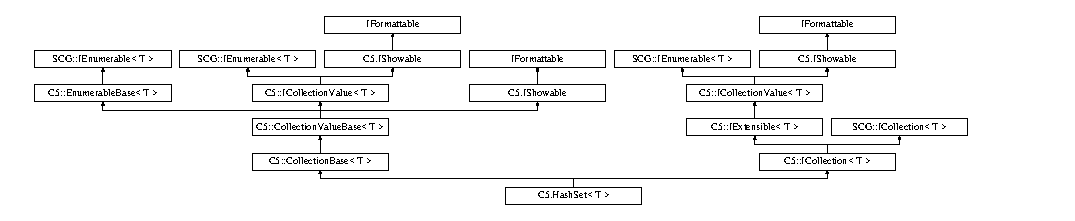
\includegraphics[height=2.526316cm]{class_c5_1_1_hash_set}
\end{center}
\end{figure}
\subsection*{Public Member Functions}
\begin{DoxyCompactItemize}
\item 
\hyperlink{class_c5_1_1_hash_set_a8c3fb4f50d669c1fe32977c8d3ef4963}{Hash\+Set} ()
\begin{DoxyCompactList}\small\item\em Create a hash set with natural item equality\+Comparer and default fill threshold (66\%) and initial table size (16). \end{DoxyCompactList}\item 
\hyperlink{class_c5_1_1_hash_set_a48ce3a77574ed39466a0a93c0543e033}{Hash\+Set} (S\+C\+G.\+I\+Equality\+Comparer$<$ T $>$ \hyperlink{class_c5_1_1_collection_base_a95e343400be0e8f3f8d6310f1aaf2cc6}{itemequality\+Comparer})
\begin{DoxyCompactList}\small\item\em Create a hash set with external item equality\+Comparer and default fill threshold (66\%) and initial table size (16). \end{DoxyCompactList}\item 
\hyperlink{class_c5_1_1_hash_set_a68917f421f09006c60050f7be04c8550}{Hash\+Set} (int capacity, S\+C\+G.\+I\+Equality\+Comparer$<$ T $>$ \hyperlink{class_c5_1_1_collection_base_a95e343400be0e8f3f8d6310f1aaf2cc6}{itemequality\+Comparer})
\begin{DoxyCompactList}\small\item\em Create a hash set with external item equality\+Comparer and default fill threshold (66\%) \end{DoxyCompactList}\item 
\hyperlink{class_c5_1_1_hash_set_acd7cc0d3e33d99fc320b9f8207650e5b}{Hash\+Set} (int capacity, double fill, S\+C\+G.\+I\+Equality\+Comparer$<$ T $>$ \hyperlink{class_c5_1_1_collection_base_a95e343400be0e8f3f8d6310f1aaf2cc6}{itemequality\+Comparer})
\begin{DoxyCompactList}\small\item\em Create a hash set with external item equality\+Comparer. \end{DoxyCompactList}\item 
virtual bool \hyperlink{class_c5_1_1_hash_set_af664a08eff9d9941c43e043bf5b367c3}{Contains} (T item)
\begin{DoxyCompactList}\small\item\em Check if an item is in the set \end{DoxyCompactList}\item 
virtual bool \hyperlink{class_c5_1_1_hash_set_a68b40c2f8c5483825915945d0f21278a}{Find} (ref T item)
\begin{DoxyCompactList}\small\item\em Check if an item (collection equal to a given one) is in the set and if so report the actual item object found. \end{DoxyCompactList}\item 
virtual bool \hyperlink{class_c5_1_1_hash_set_a0cfae793ab357695699f58064b892c8d}{Update} (T item)
\begin{DoxyCompactList}\small\item\em Check if an item (collection equal to a given one) is in the set and if so replace the item object in the set with the supplied one. \end{DoxyCompactList}\item 
virtual bool \hyperlink{class_c5_1_1_hash_set_aa0037ac87af2603ab0641e3037e5ee55}{Update} (T item, out T olditem)
\begin{DoxyCompactList}\small\item\em Check if an item (collection equal to a given one) is in the set and if so replace the item object in the set with the supplied one. \end{DoxyCompactList}\item 
virtual bool \hyperlink{class_c5_1_1_hash_set_a0b1d42cbbc91e630ab0917a2b17e8ca1}{Find\+Or\+Add} (ref T item)
\begin{DoxyCompactList}\small\item\em Check if an item (collection equal to a given one) is in the set. If found, report the actual item object in the set, else add the supplied one. \end{DoxyCompactList}\item 
virtual bool \hyperlink{class_c5_1_1_hash_set_a65709285f46c3bfd43d5dda1c4ab54fd}{Update\+Or\+Add} (T item)
\begin{DoxyCompactList}\small\item\em Check if an item (collection equal to a supplied one) is in the set and if so replace the item object in the set with the supplied one; else add the supplied one. \end{DoxyCompactList}\item 
virtual bool \hyperlink{class_c5_1_1_hash_set_a2a07fae0af3a3f329d47719019fb2c5b}{Update\+Or\+Add} (T item, out T olditem)
\begin{DoxyCompactList}\small\item\em Check if an item (collection equal to a supplied one) is in the set and if so replace the item object in the set with the supplied one; else add the supplied one. \end{DoxyCompactList}\item 
virtual bool \hyperlink{class_c5_1_1_hash_set_ac9b5cd955239472a848788ce53345853}{Remove} (T item)
\begin{DoxyCompactList}\small\item\em Remove an item from the set \end{DoxyCompactList}\item 
virtual bool \hyperlink{class_c5_1_1_hash_set_a7e97b49057ee44abddb8fbd83b56b78a}{Remove} (T item, out T removeditem)
\begin{DoxyCompactList}\small\item\em Remove an item from the set, reporting the actual matching item object. \end{DoxyCompactList}\item 
virtual void \hyperlink{class_c5_1_1_hash_set_afc71edbb94b37e74b25d0d489c36dc3b}{Remove\+All} (S\+C\+G.\+I\+Enumerable$<$ T $>$ items)
\begin{DoxyCompactList}\small\item\em Remove all items in a supplied collection from this set. \end{DoxyCompactList}\item 
virtual void \hyperlink{class_c5_1_1_hash_set_a7bc97cd3a07e8e829c16e169ac71a075}{Clear} ()
\begin{DoxyCompactList}\small\item\em Remove all items from the set, resetting internal table to initial size. \end{DoxyCompactList}\item 
virtual void \hyperlink{class_c5_1_1_hash_set_a5ab8110d40df588e0214b2d55eb085ce}{Retain\+All} (S\+C\+G.\+I\+Enumerable$<$ T $>$ items)
\begin{DoxyCompactList}\small\item\em Remove all items {\itshape not} in a supplied collection from this set. \end{DoxyCompactList}\item 
virtual bool \hyperlink{class_c5_1_1_hash_set_ad7c29ad00f9697d4a07e03986c84770e}{Contains\+All} (S\+C\+G.\+I\+Enumerable$<$ T $>$ items)
\begin{DoxyCompactList}\small\item\em Check if all items in a supplied collection is in this set (ignoring multiplicities). \end{DoxyCompactList}\item 
override T\mbox{[}$\,$\mbox{]} \hyperlink{class_c5_1_1_hash_set_ad6e22ebc64d9f8c96b805547d5873023}{To\+Array} ()
\begin{DoxyCompactList}\small\item\em Create an array containing all items in this set (in enumeration order). \end{DoxyCompactList}\item 
virtual int \hyperlink{class_c5_1_1_hash_set_a6ae7c12192030c64a6268546bdb21fbe}{Contains\+Count} (T item)
\begin{DoxyCompactList}\small\item\em Count the number of times an item is in this set (either 0 or 1). \end{DoxyCompactList}\item 
virtual \hyperlink{interface_c5_1_1_i_collection_value}{I\+Collection\+Value}$<$ T $>$ \hyperlink{class_c5_1_1_hash_set_a8f1963ae2661d4b9b064f88124789c76}{Unique\+Items} ()
\item 
virtual \hyperlink{interface_c5_1_1_i_collection_value}{I\+Collection\+Value}$<$ \hyperlink{struct_c5_1_1_key_value_pair}{Key\+Value\+Pair}$<$ T, int $>$ $>$ \hyperlink{class_c5_1_1_hash_set_ae8e2ee2134a81967efe6fef79d67a0fc}{Item\+Multiplicities} ()
\item 
virtual void \hyperlink{class_c5_1_1_hash_set_a07eacbcc5850774881dd596676e6b134}{Remove\+All\+Copies} (T item)
\begin{DoxyCompactList}\small\item\em Remove all (at most 1) copies of item from this set. \end{DoxyCompactList}\item 
override T \hyperlink{class_c5_1_1_hash_set_a6bac17b51f5b2a569a0df8e0c46fe78f}{Choose} ()
\begin{DoxyCompactList}\small\item\em Choose some item of this collection. \end{DoxyCompactList}\item 
override S\+C\+G.\+I\+Enumerator$<$ T $>$ \hyperlink{class_c5_1_1_hash_set_a4c404a22695abc0f6b47bf74d3d34034}{Get\+Enumerator} ()
\begin{DoxyCompactList}\small\item\em Create an enumerator for this set. \end{DoxyCompactList}\item 
virtual bool \hyperlink{class_c5_1_1_hash_set_a0700ad4332214ac5d74f3a197bfd8774}{Add} (T item)
\begin{DoxyCompactList}\small\item\em Add an item to this set. \end{DoxyCompactList}\item 
virtual void \hyperlink{class_c5_1_1_hash_set_aabee06dcd4be050a024c507e781d338e}{Add\+All} (S\+C\+G.\+I\+Enumerable$<$ T $>$ items)
\begin{DoxyCompactList}\small\item\em Add the elements from another collection with a more specialized item type to this collection. Since this collection has set semantics, only items not already in the collection will be added. \end{DoxyCompactList}\item 
virtual bool \hyperlink{class_c5_1_1_hash_set_a7000a1b6fea242f1f5ca40571724b309}{Check} ()
\begin{DoxyCompactList}\small\item\em Test internal structure of data (invariants) \end{DoxyCompactList}\item 
\hyperlink{interface_c5_1_1_i_sorted_dictionary}{I\+Sorted\+Dictionary}$<$ int, int $>$ \hyperlink{class_c5_1_1_hash_set_aa85358a09cbd7316bfad33a79dbc69e4}{Bucket\+Cost\+Distribution} ()
\begin{DoxyCompactList}\small\item\em Produce statistics on distribution of bucket sizes. Current implementation is incomplete. \end{DoxyCompactList}\end{DoxyCompactItemize}
\subsection*{Properties}
\begin{DoxyCompactItemize}
\item 
static \hyperlink{_hash_table_8cs_a3ba53141e4e2a9f89bcfc8cf229955f7}{Feature} \hyperlink{class_c5_1_1_hash_set_af105c294816c484c8e48544daa7c0b32}{Features}\hspace{0.3cm}{\ttfamily  \mbox{[}get\mbox{]}}
\begin{DoxyCompactList}\small\item\em Show which implementation features was chosen at compilation time \end{DoxyCompactList}\item 
override \hyperlink{namespace_c5_a9143bfd561fffa025d21561674758008}{Event\+Type\+Enum} \hyperlink{class_c5_1_1_hash_set_a55a5a5a8a33bd7058881493bc3d3ae6a}{Listenable\+Events}\hspace{0.3cm}{\ttfamily  \mbox{[}get\mbox{]}}
\item 
virtual \hyperlink{namespace_c5_a615ba88dcdaa8d5a3c5f833a73d7fad6}{Speed} \hyperlink{class_c5_1_1_hash_set_a206298276b5ddfbb9a528df96a5620ae}{Contains\+Speed}\hspace{0.3cm}{\ttfamily  \mbox{[}get\mbox{]}}
\begin{DoxyCompactList}\small\item\em The complexity of the Contains operation \end{DoxyCompactList}\item 
virtual bool \hyperlink{class_c5_1_1_hash_set_a95849b8404288074ea8622d77ccb1142}{Allows\+Duplicates}\hspace{0.3cm}{\ttfamily  \mbox{[}get\mbox{]}}
\begin{DoxyCompactList}\small\item\em Report if this is a set collection. \end{DoxyCompactList}\item 
virtual bool \hyperlink{class_c5_1_1_hash_set_ae9ad56098db41bbbd2a0baabef06bc14}{Duplicates\+By\+Counting}\hspace{0.3cm}{\ttfamily  \mbox{[}get\mbox{]}}
\begin{DoxyCompactList}\small\item\em By convention this is true for any collection with set semantics. \end{DoxyCompactList}\end{DoxyCompactItemize}
\subsection*{Additional Inherited Members}


\subsection{Detailed Description}
A set collection class based on linear hashing 



\subsection{Constructor \& Destructor Documentation}
\hypertarget{class_c5_1_1_hash_set_a8c3fb4f50d669c1fe32977c8d3ef4963}{}\index{C5\+::\+Hash\+Set@{C5\+::\+Hash\+Set}!Hash\+Set@{Hash\+Set}}
\index{Hash\+Set@{Hash\+Set}!C5\+::\+Hash\+Set@{C5\+::\+Hash\+Set}}
\subsubsection[{Hash\+Set()}]{\setlength{\rightskip}{0pt plus 5cm}{\bf C5.\+Hash\+Set}$<$ T $>$.{\bf Hash\+Set} (
\begin{DoxyParamCaption}
{}
\end{DoxyParamCaption}
)}\label{class_c5_1_1_hash_set_a8c3fb4f50d669c1fe32977c8d3ef4963}


Create a hash set with natural item equality\+Comparer and default fill threshold (66\%) and initial table size (16). 

\hypertarget{class_c5_1_1_hash_set_a48ce3a77574ed39466a0a93c0543e033}{}\index{C5\+::\+Hash\+Set@{C5\+::\+Hash\+Set}!Hash\+Set@{Hash\+Set}}
\index{Hash\+Set@{Hash\+Set}!C5\+::\+Hash\+Set@{C5\+::\+Hash\+Set}}
\subsubsection[{Hash\+Set(\+S\+C\+G.\+I\+Equality\+Comparer$<$ T $>$ itemequality\+Comparer)}]{\setlength{\rightskip}{0pt plus 5cm}{\bf C5.\+Hash\+Set}$<$ T $>$.{\bf Hash\+Set} (
\begin{DoxyParamCaption}
\item[{S\+C\+G.\+I\+Equality\+Comparer$<$ T $>$}]{itemequality\+Comparer}
\end{DoxyParamCaption}
)}\label{class_c5_1_1_hash_set_a48ce3a77574ed39466a0a93c0543e033}


Create a hash set with external item equality\+Comparer and default fill threshold (66\%) and initial table size (16). 


\begin{DoxyParams}{Parameters}
{\em itemequality\+Comparer} & The external item equality\+S\+C\+G.\+Comparer\\
\hline
\end{DoxyParams}
\hypertarget{class_c5_1_1_hash_set_a68917f421f09006c60050f7be04c8550}{}\index{C5\+::\+Hash\+Set@{C5\+::\+Hash\+Set}!Hash\+Set@{Hash\+Set}}
\index{Hash\+Set@{Hash\+Set}!C5\+::\+Hash\+Set@{C5\+::\+Hash\+Set}}
\subsubsection[{Hash\+Set(int capacity, S\+C\+G.\+I\+Equality\+Comparer$<$ T $>$ itemequality\+Comparer)}]{\setlength{\rightskip}{0pt plus 5cm}{\bf C5.\+Hash\+Set}$<$ T $>$.{\bf Hash\+Set} (
\begin{DoxyParamCaption}
\item[{int}]{capacity, }
\item[{S\+C\+G.\+I\+Equality\+Comparer$<$ T $>$}]{itemequality\+Comparer}
\end{DoxyParamCaption}
)}\label{class_c5_1_1_hash_set_a68917f421f09006c60050f7be04c8550}


Create a hash set with external item equality\+Comparer and default fill threshold (66\%) 


\begin{DoxyParams}{Parameters}
{\em capacity} & Initial table size (rounded to power of 2, at least 16)\\
\hline
{\em itemequality\+Comparer} & The external item equality\+S\+C\+G.\+Comparer\\
\hline
\end{DoxyParams}
\hypertarget{class_c5_1_1_hash_set_acd7cc0d3e33d99fc320b9f8207650e5b}{}\index{C5\+::\+Hash\+Set@{C5\+::\+Hash\+Set}!Hash\+Set@{Hash\+Set}}
\index{Hash\+Set@{Hash\+Set}!C5\+::\+Hash\+Set@{C5\+::\+Hash\+Set}}
\subsubsection[{Hash\+Set(int capacity, double fill, S\+C\+G.\+I\+Equality\+Comparer$<$ T $>$ itemequality\+Comparer)}]{\setlength{\rightskip}{0pt plus 5cm}{\bf C5.\+Hash\+Set}$<$ T $>$.{\bf Hash\+Set} (
\begin{DoxyParamCaption}
\item[{int}]{capacity, }
\item[{double}]{fill, }
\item[{S\+C\+G.\+I\+Equality\+Comparer$<$ T $>$}]{itemequality\+Comparer}
\end{DoxyParamCaption}
)}\label{class_c5_1_1_hash_set_acd7cc0d3e33d99fc320b9f8207650e5b}


Create a hash set with external item equality\+Comparer. 


\begin{DoxyParams}{Parameters}
{\em capacity} & Initial table size (rounded to power of 2, at least 16)\\
\hline
{\em fill} & Fill threshold (in range 10\% to 90\%)\\
\hline
{\em itemequality\+Comparer} & The external item equality\+S\+C\+G.\+Comparer\\
\hline
\end{DoxyParams}


\subsection{Member Function Documentation}
\hypertarget{class_c5_1_1_hash_set_a0700ad4332214ac5d74f3a197bfd8774}{}\index{C5\+::\+Hash\+Set@{C5\+::\+Hash\+Set}!Add@{Add}}
\index{Add@{Add}!C5\+::\+Hash\+Set@{C5\+::\+Hash\+Set}}
\subsubsection[{Add(\+T item)}]{\setlength{\rightskip}{0pt plus 5cm}virtual bool {\bf C5.\+Hash\+Set}$<$ T $>$.Add (
\begin{DoxyParamCaption}
\item[{T}]{item}
\end{DoxyParamCaption}
)\hspace{0.3cm}{\ttfamily [virtual]}}\label{class_c5_1_1_hash_set_a0700ad4332214ac5d74f3a197bfd8774}


Add an item to this set. 


\begin{DoxyParams}{Parameters}
{\em item} & The item to add.\\
\hline
\end{DoxyParams}
\begin{DoxyReturn}{Returns}
True if item was added (i.\+e. not found)
\end{DoxyReturn}


Implements \hyperlink{interface_c5_1_1_i_collection_a525115f252ddca586fcbf1a0127be614}{C5.\+I\+Collection$<$ T $>$}.

\hypertarget{class_c5_1_1_hash_set_aabee06dcd4be050a024c507e781d338e}{}\index{C5\+::\+Hash\+Set@{C5\+::\+Hash\+Set}!Add\+All@{Add\+All}}
\index{Add\+All@{Add\+All}!C5\+::\+Hash\+Set@{C5\+::\+Hash\+Set}}
\subsubsection[{Add\+All(\+S\+C\+G.\+I\+Enumerable$<$ T $>$ items)}]{\setlength{\rightskip}{0pt plus 5cm}virtual void {\bf C5.\+Hash\+Set}$<$ T $>$.Add\+All (
\begin{DoxyParamCaption}
\item[{S\+C\+G.\+I\+Enumerable$<$ T $>$}]{items}
\end{DoxyParamCaption}
)\hspace{0.3cm}{\ttfamily [virtual]}}\label{class_c5_1_1_hash_set_aabee06dcd4be050a024c507e781d338e}


Add the elements from another collection with a more specialized item type to this collection. Since this collection has set semantics, only items not already in the collection will be added. 


\begin{DoxyParams}{Parameters}
{\em items} & The items to add\\
\hline
\end{DoxyParams}


Implements \hyperlink{interface_c5_1_1_i_extensible_a1fb4d50c5b340e60303da72e9d0ede6e}{C5.\+I\+Extensible$<$ T $>$}.

\hypertarget{class_c5_1_1_hash_set_aa85358a09cbd7316bfad33a79dbc69e4}{}\index{C5\+::\+Hash\+Set@{C5\+::\+Hash\+Set}!Bucket\+Cost\+Distribution@{Bucket\+Cost\+Distribution}}
\index{Bucket\+Cost\+Distribution@{Bucket\+Cost\+Distribution}!C5\+::\+Hash\+Set@{C5\+::\+Hash\+Set}}
\subsubsection[{Bucket\+Cost\+Distribution()}]{\setlength{\rightskip}{0pt plus 5cm}{\bf I\+Sorted\+Dictionary}$<$int, int$>$ {\bf C5.\+Hash\+Set}$<$ T $>$.Bucket\+Cost\+Distribution (
\begin{DoxyParamCaption}
{}
\end{DoxyParamCaption}
)}\label{class_c5_1_1_hash_set_aa85358a09cbd7316bfad33a79dbc69e4}


Produce statistics on distribution of bucket sizes. Current implementation is incomplete. 

\begin{DoxyReturn}{Returns}
Histogram data.
\end{DoxyReturn}
\hypertarget{class_c5_1_1_hash_set_a7000a1b6fea242f1f5ca40571724b309}{}\index{C5\+::\+Hash\+Set@{C5\+::\+Hash\+Set}!Check@{Check}}
\index{Check@{Check}!C5\+::\+Hash\+Set@{C5\+::\+Hash\+Set}}
\subsubsection[{Check()}]{\setlength{\rightskip}{0pt plus 5cm}virtual bool {\bf C5.\+Hash\+Set}$<$ T $>$.Check (
\begin{DoxyParamCaption}
{}
\end{DoxyParamCaption}
)\hspace{0.3cm}{\ttfamily [virtual]}}\label{class_c5_1_1_hash_set_a7000a1b6fea242f1f5ca40571724b309}


Test internal structure of data (invariants) 

\begin{DoxyReturn}{Returns}
True if pass
\end{DoxyReturn}


Implements \hyperlink{interface_c5_1_1_i_extensible_aeeb6b87af61e455df42d68834d711bcb}{C5.\+I\+Extensible$<$ T $>$}.

\hypertarget{class_c5_1_1_hash_set_a6bac17b51f5b2a569a0df8e0c46fe78f}{}\index{C5\+::\+Hash\+Set@{C5\+::\+Hash\+Set}!Choose@{Choose}}
\index{Choose@{Choose}!C5\+::\+Hash\+Set@{C5\+::\+Hash\+Set}}
\subsubsection[{Choose()}]{\setlength{\rightskip}{0pt plus 5cm}override T {\bf C5.\+Hash\+Set}$<$ T $>$.Choose (
\begin{DoxyParamCaption}
{}
\end{DoxyParamCaption}
)\hspace{0.3cm}{\ttfamily [virtual]}}\label{class_c5_1_1_hash_set_a6bac17b51f5b2a569a0df8e0c46fe78f}


Choose some item of this collection. 


\begin{DoxyExceptions}{Exceptions}
{\em \hyperlink{class_c5_1_1_no_such_item_exception}{No\+Such\+Item\+Exception}} & if collection is empty.\\
\hline
\end{DoxyExceptions}
\begin{DoxyReturn}{Returns}

\end{DoxyReturn}


Implements \hyperlink{class_c5_1_1_collection_value_base_ad7b8bd01dfd7ea8480a972f02a81608b}{C5.\+Collection\+Value\+Base$<$ T $>$}.

\hypertarget{class_c5_1_1_hash_set_a7bc97cd3a07e8e829c16e169ac71a075}{}\index{C5\+::\+Hash\+Set@{C5\+::\+Hash\+Set}!Clear@{Clear}}
\index{Clear@{Clear}!C5\+::\+Hash\+Set@{C5\+::\+Hash\+Set}}
\subsubsection[{Clear()}]{\setlength{\rightskip}{0pt plus 5cm}virtual void {\bf C5.\+Hash\+Set}$<$ T $>$.Clear (
\begin{DoxyParamCaption}
{}
\end{DoxyParamCaption}
)\hspace{0.3cm}{\ttfamily [virtual]}}\label{class_c5_1_1_hash_set_a7bc97cd3a07e8e829c16e169ac71a075}


Remove all items from the set, resetting internal table to initial size. 



Implements \hyperlink{interface_c5_1_1_i_collection_abd83166ac00b3d36225d988fd4603e97}{C5.\+I\+Collection$<$ T $>$}.

\hypertarget{class_c5_1_1_hash_set_af664a08eff9d9941c43e043bf5b367c3}{}\index{C5\+::\+Hash\+Set@{C5\+::\+Hash\+Set}!Contains@{Contains}}
\index{Contains@{Contains}!C5\+::\+Hash\+Set@{C5\+::\+Hash\+Set}}
\subsubsection[{Contains(\+T item)}]{\setlength{\rightskip}{0pt plus 5cm}virtual bool {\bf C5.\+Hash\+Set}$<$ T $>$.Contains (
\begin{DoxyParamCaption}
\item[{T}]{item}
\end{DoxyParamCaption}
)\hspace{0.3cm}{\ttfamily [virtual]}}\label{class_c5_1_1_hash_set_af664a08eff9d9941c43e043bf5b367c3}


Check if an item is in the set 


\begin{DoxyParams}{Parameters}
{\em item} & The item to look for\\
\hline
\end{DoxyParams}
\begin{DoxyReturn}{Returns}
True if set contains item
\end{DoxyReturn}


Implements \hyperlink{interface_c5_1_1_i_collection_a4de01b6d77ea5eaffccc8267b4454cdd}{C5.\+I\+Collection$<$ T $>$}.

\hypertarget{class_c5_1_1_hash_set_ad7c29ad00f9697d4a07e03986c84770e}{}\index{C5\+::\+Hash\+Set@{C5\+::\+Hash\+Set}!Contains\+All@{Contains\+All}}
\index{Contains\+All@{Contains\+All}!C5\+::\+Hash\+Set@{C5\+::\+Hash\+Set}}
\subsubsection[{Contains\+All(\+S\+C\+G.\+I\+Enumerable$<$ T $>$ items)}]{\setlength{\rightskip}{0pt plus 5cm}virtual bool {\bf C5.\+Hash\+Set}$<$ T $>$.Contains\+All (
\begin{DoxyParamCaption}
\item[{S\+C\+G.\+I\+Enumerable$<$ T $>$}]{items}
\end{DoxyParamCaption}
)\hspace{0.3cm}{\ttfamily [virtual]}}\label{class_c5_1_1_hash_set_ad7c29ad00f9697d4a07e03986c84770e}


Check if all items in a supplied collection is in this set (ignoring multiplicities). 


\begin{DoxyParams}{Parameters}
{\em items} & The items to look for.\\
\hline
\end{DoxyParams}
\begin{DoxyReturn}{Returns}
True if all items are found.
\end{DoxyReturn}


Implements \hyperlink{interface_c5_1_1_i_collection_a93abf02183a46f56af8d90f1d69982a8}{C5.\+I\+Collection$<$ T $>$}.

\hypertarget{class_c5_1_1_hash_set_a6ae7c12192030c64a6268546bdb21fbe}{}\index{C5\+::\+Hash\+Set@{C5\+::\+Hash\+Set}!Contains\+Count@{Contains\+Count}}
\index{Contains\+Count@{Contains\+Count}!C5\+::\+Hash\+Set@{C5\+::\+Hash\+Set}}
\subsubsection[{Contains\+Count(\+T item)}]{\setlength{\rightskip}{0pt plus 5cm}virtual int {\bf C5.\+Hash\+Set}$<$ T $>$.Contains\+Count (
\begin{DoxyParamCaption}
\item[{T}]{item}
\end{DoxyParamCaption}
)\hspace{0.3cm}{\ttfamily [virtual]}}\label{class_c5_1_1_hash_set_a6ae7c12192030c64a6268546bdb21fbe}


Count the number of times an item is in this set (either 0 or 1). 


\begin{DoxyParams}{Parameters}
{\em item} & The item to look for.\\
\hline
\end{DoxyParams}
\begin{DoxyReturn}{Returns}
1 if item is in set, 0 else
\end{DoxyReturn}


Implements \hyperlink{interface_c5_1_1_i_collection_acfe7e2c9b14c384762269edbb57b7fbe}{C5.\+I\+Collection$<$ T $>$}.

\hypertarget{class_c5_1_1_hash_set_a68b40c2f8c5483825915945d0f21278a}{}\index{C5\+::\+Hash\+Set@{C5\+::\+Hash\+Set}!Find@{Find}}
\index{Find@{Find}!C5\+::\+Hash\+Set@{C5\+::\+Hash\+Set}}
\subsubsection[{Find(ref T item)}]{\setlength{\rightskip}{0pt plus 5cm}virtual bool {\bf C5.\+Hash\+Set}$<$ T $>$.Find (
\begin{DoxyParamCaption}
\item[{ref T}]{item}
\end{DoxyParamCaption}
)\hspace{0.3cm}{\ttfamily [virtual]}}\label{class_c5_1_1_hash_set_a68b40c2f8c5483825915945d0f21278a}


Check if an item (collection equal to a given one) is in the set and if so report the actual item object found. 


\begin{DoxyParams}{Parameters}
{\em item} & On entry, the item to look for. On exit the item found, if any\\
\hline
\end{DoxyParams}
\begin{DoxyReturn}{Returns}
True if set contains item
\end{DoxyReturn}


Implements \hyperlink{interface_c5_1_1_i_collection_a96fd6cfd3df62e67922f9335b0fbbdcb}{C5.\+I\+Collection$<$ T $>$}.

\hypertarget{class_c5_1_1_hash_set_a0b1d42cbbc91e630ab0917a2b17e8ca1}{}\index{C5\+::\+Hash\+Set@{C5\+::\+Hash\+Set}!Find\+Or\+Add@{Find\+Or\+Add}}
\index{Find\+Or\+Add@{Find\+Or\+Add}!C5\+::\+Hash\+Set@{C5\+::\+Hash\+Set}}
\subsubsection[{Find\+Or\+Add(ref T item)}]{\setlength{\rightskip}{0pt plus 5cm}virtual bool {\bf C5.\+Hash\+Set}$<$ T $>$.Find\+Or\+Add (
\begin{DoxyParamCaption}
\item[{ref T}]{item}
\end{DoxyParamCaption}
)\hspace{0.3cm}{\ttfamily [virtual]}}\label{class_c5_1_1_hash_set_a0b1d42cbbc91e630ab0917a2b17e8ca1}


Check if an item (collection equal to a given one) is in the set. If found, report the actual item object in the set, else add the supplied one. 


\begin{DoxyParams}{Parameters}
{\em item} & On entry, the item to look for or add. On exit the actual object found, if any.\\
\hline
\end{DoxyParams}
\begin{DoxyReturn}{Returns}
True if item was found
\end{DoxyReturn}


Implements \hyperlink{interface_c5_1_1_i_collection_a7f9e609ee1a7607596bb65aa5bdff303}{C5.\+I\+Collection$<$ T $>$}.

\hypertarget{class_c5_1_1_hash_set_a4c404a22695abc0f6b47bf74d3d34034}{}\index{C5\+::\+Hash\+Set@{C5\+::\+Hash\+Set}!Get\+Enumerator@{Get\+Enumerator}}
\index{Get\+Enumerator@{Get\+Enumerator}!C5\+::\+Hash\+Set@{C5\+::\+Hash\+Set}}
\subsubsection[{Get\+Enumerator()}]{\setlength{\rightskip}{0pt plus 5cm}override S\+C\+G.\+I\+Enumerator$<$T$>$ {\bf C5.\+Hash\+Set}$<$ T $>$.Get\+Enumerator (
\begin{DoxyParamCaption}
{}
\end{DoxyParamCaption}
)\hspace{0.3cm}{\ttfamily [virtual]}}\label{class_c5_1_1_hash_set_a4c404a22695abc0f6b47bf74d3d34034}


Create an enumerator for this set. 

\begin{DoxyReturn}{Returns}
The enumerator
\end{DoxyReturn}


Implements \hyperlink{class_c5_1_1_collection_base_a3b4b98e2606afecb948019412c4c2533}{C5.\+Collection\+Base$<$ T $>$}.

\hypertarget{class_c5_1_1_hash_set_ae8e2ee2134a81967efe6fef79d67a0fc}{}\index{C5\+::\+Hash\+Set@{C5\+::\+Hash\+Set}!Item\+Multiplicities@{Item\+Multiplicities}}
\index{Item\+Multiplicities@{Item\+Multiplicities}!C5\+::\+Hash\+Set@{C5\+::\+Hash\+Set}}
\subsubsection[{Item\+Multiplicities()}]{\setlength{\rightskip}{0pt plus 5cm}virtual {\bf I\+Collection\+Value}$<${\bf Key\+Value\+Pair}$<$T, int$>$ $>$ {\bf C5.\+Hash\+Set}$<$ T $>$.Item\+Multiplicities (
\begin{DoxyParamCaption}
{}
\end{DoxyParamCaption}
)\hspace{0.3cm}{\ttfamily [virtual]}}\label{class_c5_1_1_hash_set_ae8e2ee2134a81967efe6fef79d67a0fc}




\begin{DoxyReturn}{Returns}

\end{DoxyReturn}


Implements \hyperlink{interface_c5_1_1_i_collection_a623bd834b37b299c5f4948fdb6915fef}{C5.\+I\+Collection$<$ T $>$}.

\hypertarget{class_c5_1_1_hash_set_ac9b5cd955239472a848788ce53345853}{}\index{C5\+::\+Hash\+Set@{C5\+::\+Hash\+Set}!Remove@{Remove}}
\index{Remove@{Remove}!C5\+::\+Hash\+Set@{C5\+::\+Hash\+Set}}
\subsubsection[{Remove(\+T item)}]{\setlength{\rightskip}{0pt plus 5cm}virtual bool {\bf C5.\+Hash\+Set}$<$ T $>$.Remove (
\begin{DoxyParamCaption}
\item[{T}]{item}
\end{DoxyParamCaption}
)\hspace{0.3cm}{\ttfamily [virtual]}}\label{class_c5_1_1_hash_set_ac9b5cd955239472a848788ce53345853}


Remove an item from the set 


\begin{DoxyParams}{Parameters}
{\em item} & The item to remove\\
\hline
\end{DoxyParams}
\begin{DoxyReturn}{Returns}
True if item was (found and) removed 
\end{DoxyReturn}


Implements \hyperlink{interface_c5_1_1_i_collection_ab4d6092ac09245ce46db91595fc1cdfe}{C5.\+I\+Collection$<$ T $>$}.

\hypertarget{class_c5_1_1_hash_set_a7e97b49057ee44abddb8fbd83b56b78a}{}\index{C5\+::\+Hash\+Set@{C5\+::\+Hash\+Set}!Remove@{Remove}}
\index{Remove@{Remove}!C5\+::\+Hash\+Set@{C5\+::\+Hash\+Set}}
\subsubsection[{Remove(\+T item, out T removeditem)}]{\setlength{\rightskip}{0pt plus 5cm}virtual bool {\bf C5.\+Hash\+Set}$<$ T $>$.Remove (
\begin{DoxyParamCaption}
\item[{T}]{item, }
\item[{out T}]{removeditem}
\end{DoxyParamCaption}
)\hspace{0.3cm}{\ttfamily [virtual]}}\label{class_c5_1_1_hash_set_a7e97b49057ee44abddb8fbd83b56b78a}


Remove an item from the set, reporting the actual matching item object. 


\begin{DoxyParams}{Parameters}
{\em item} & The value to remove.\\
\hline
{\em removeditem} & The removed value.\\
\hline
\end{DoxyParams}
\begin{DoxyReturn}{Returns}
True if item was found.
\end{DoxyReturn}


Implements \hyperlink{interface_c5_1_1_i_collection_acbd124236c3f0958a8784d9c7c2dfd16}{C5.\+I\+Collection$<$ T $>$}.

\hypertarget{class_c5_1_1_hash_set_afc71edbb94b37e74b25d0d489c36dc3b}{}\index{C5\+::\+Hash\+Set@{C5\+::\+Hash\+Set}!Remove\+All@{Remove\+All}}
\index{Remove\+All@{Remove\+All}!C5\+::\+Hash\+Set@{C5\+::\+Hash\+Set}}
\subsubsection[{Remove\+All(\+S\+C\+G.\+I\+Enumerable$<$ T $>$ items)}]{\setlength{\rightskip}{0pt plus 5cm}virtual void {\bf C5.\+Hash\+Set}$<$ T $>$.Remove\+All (
\begin{DoxyParamCaption}
\item[{S\+C\+G.\+I\+Enumerable$<$ T $>$}]{items}
\end{DoxyParamCaption}
)\hspace{0.3cm}{\ttfamily [virtual]}}\label{class_c5_1_1_hash_set_afc71edbb94b37e74b25d0d489c36dc3b}


Remove all items in a supplied collection from this set. 


\begin{DoxyParams}{Parameters}
{\em items} & The items to remove.\\
\hline
\end{DoxyParams}


Implements \hyperlink{interface_c5_1_1_i_collection_a9fb05163a1bd4b71bfd05101ff20c987}{C5.\+I\+Collection$<$ T $>$}.

\hypertarget{class_c5_1_1_hash_set_a07eacbcc5850774881dd596676e6b134}{}\index{C5\+::\+Hash\+Set@{C5\+::\+Hash\+Set}!Remove\+All\+Copies@{Remove\+All\+Copies}}
\index{Remove\+All\+Copies@{Remove\+All\+Copies}!C5\+::\+Hash\+Set@{C5\+::\+Hash\+Set}}
\subsubsection[{Remove\+All\+Copies(\+T item)}]{\setlength{\rightskip}{0pt plus 5cm}virtual void {\bf C5.\+Hash\+Set}$<$ T $>$.Remove\+All\+Copies (
\begin{DoxyParamCaption}
\item[{T}]{item}
\end{DoxyParamCaption}
)\hspace{0.3cm}{\ttfamily [virtual]}}\label{class_c5_1_1_hash_set_a07eacbcc5850774881dd596676e6b134}


Remove all (at most 1) copies of item from this set. 


\begin{DoxyParams}{Parameters}
{\em item} & The item to remove\\
\hline
\end{DoxyParams}


Implements \hyperlink{interface_c5_1_1_i_collection_ad785b91be4edeb3fbe678db751f6355d}{C5.\+I\+Collection$<$ T $>$}.

\hypertarget{class_c5_1_1_hash_set_a5ab8110d40df588e0214b2d55eb085ce}{}\index{C5\+::\+Hash\+Set@{C5\+::\+Hash\+Set}!Retain\+All@{Retain\+All}}
\index{Retain\+All@{Retain\+All}!C5\+::\+Hash\+Set@{C5\+::\+Hash\+Set}}
\subsubsection[{Retain\+All(\+S\+C\+G.\+I\+Enumerable$<$ T $>$ items)}]{\setlength{\rightskip}{0pt plus 5cm}virtual void {\bf C5.\+Hash\+Set}$<$ T $>$.Retain\+All (
\begin{DoxyParamCaption}
\item[{S\+C\+G.\+I\+Enumerable$<$ T $>$}]{items}
\end{DoxyParamCaption}
)\hspace{0.3cm}{\ttfamily [virtual]}}\label{class_c5_1_1_hash_set_a5ab8110d40df588e0214b2d55eb085ce}


Remove all items {\itshape not} in a supplied collection from this set. 


\begin{DoxyParams}{Parameters}
{\em items} & The items to retain\\
\hline
\end{DoxyParams}


Implements \hyperlink{interface_c5_1_1_i_collection_ac2672fb0557eeb24e328149c513c9a8b}{C5.\+I\+Collection$<$ T $>$}.

\hypertarget{class_c5_1_1_hash_set_ad6e22ebc64d9f8c96b805547d5873023}{}\index{C5\+::\+Hash\+Set@{C5\+::\+Hash\+Set}!To\+Array@{To\+Array}}
\index{To\+Array@{To\+Array}!C5\+::\+Hash\+Set@{C5\+::\+Hash\+Set}}
\subsubsection[{To\+Array()}]{\setlength{\rightskip}{0pt plus 5cm}override T \mbox{[}$\,$\mbox{]} {\bf C5.\+Hash\+Set}$<$ T $>$.To\+Array (
\begin{DoxyParamCaption}
{}
\end{DoxyParamCaption}
)\hspace{0.3cm}{\ttfamily [virtual]}}\label{class_c5_1_1_hash_set_ad6e22ebc64d9f8c96b805547d5873023}


Create an array containing all items in this set (in enumeration order). 

\begin{DoxyReturn}{Returns}
The array
\end{DoxyReturn}


Reimplemented from \hyperlink{class_c5_1_1_collection_value_base_a740757aebaa1365811e76729e59f338d}{C5.\+Collection\+Value\+Base$<$ T $>$}.

\hypertarget{class_c5_1_1_hash_set_a8f1963ae2661d4b9b064f88124789c76}{}\index{C5\+::\+Hash\+Set@{C5\+::\+Hash\+Set}!Unique\+Items@{Unique\+Items}}
\index{Unique\+Items@{Unique\+Items}!C5\+::\+Hash\+Set@{C5\+::\+Hash\+Set}}
\subsubsection[{Unique\+Items()}]{\setlength{\rightskip}{0pt plus 5cm}virtual {\bf I\+Collection\+Value}$<$T$>$ {\bf C5.\+Hash\+Set}$<$ T $>$.Unique\+Items (
\begin{DoxyParamCaption}
{}
\end{DoxyParamCaption}
)\hspace{0.3cm}{\ttfamily [virtual]}}\label{class_c5_1_1_hash_set_a8f1963ae2661d4b9b064f88124789c76}




\begin{DoxyReturn}{Returns}

\end{DoxyReturn}


Implements \hyperlink{interface_c5_1_1_i_collection_a074c4e1a90fb7f98c95834204352c28c}{C5.\+I\+Collection$<$ T $>$}.

\hypertarget{class_c5_1_1_hash_set_a0cfae793ab357695699f58064b892c8d}{}\index{C5\+::\+Hash\+Set@{C5\+::\+Hash\+Set}!Update@{Update}}
\index{Update@{Update}!C5\+::\+Hash\+Set@{C5\+::\+Hash\+Set}}
\subsubsection[{Update(\+T item)}]{\setlength{\rightskip}{0pt plus 5cm}virtual bool {\bf C5.\+Hash\+Set}$<$ T $>$.Update (
\begin{DoxyParamCaption}
\item[{T}]{item}
\end{DoxyParamCaption}
)\hspace{0.3cm}{\ttfamily [virtual]}}\label{class_c5_1_1_hash_set_a0cfae793ab357695699f58064b892c8d}


Check if an item (collection equal to a given one) is in the set and if so replace the item object in the set with the supplied one. 


\begin{DoxyParams}{Parameters}
{\em item} & The item object to update with\\
\hline
\end{DoxyParams}
\begin{DoxyReturn}{Returns}
True if item was found (and updated)
\end{DoxyReturn}


Implements \hyperlink{interface_c5_1_1_i_collection_acf060ba6b83289dc74bea61502318d56}{C5.\+I\+Collection$<$ T $>$}.

\hypertarget{class_c5_1_1_hash_set_aa0037ac87af2603ab0641e3037e5ee55}{}\index{C5\+::\+Hash\+Set@{C5\+::\+Hash\+Set}!Update@{Update}}
\index{Update@{Update}!C5\+::\+Hash\+Set@{C5\+::\+Hash\+Set}}
\subsubsection[{Update(\+T item, out T olditem)}]{\setlength{\rightskip}{0pt plus 5cm}virtual bool {\bf C5.\+Hash\+Set}$<$ T $>$.Update (
\begin{DoxyParamCaption}
\item[{T}]{item, }
\item[{out T}]{olditem}
\end{DoxyParamCaption}
)\hspace{0.3cm}{\ttfamily [virtual]}}\label{class_c5_1_1_hash_set_aa0037ac87af2603ab0641e3037e5ee55}


Check if an item (collection equal to a given one) is in the set and if so replace the item object in the set with the supplied one. 


\begin{DoxyParams}{Parameters}
{\em item} & The item object to update with\\
\hline
{\em olditem} & \\
\hline
\end{DoxyParams}
\begin{DoxyReturn}{Returns}
True if item was found (and updated)
\end{DoxyReturn}


Implements \hyperlink{interface_c5_1_1_i_collection_ad1faa1738e02acf001aac16a3b948c78}{C5.\+I\+Collection$<$ T $>$}.

\hypertarget{class_c5_1_1_hash_set_a65709285f46c3bfd43d5dda1c4ab54fd}{}\index{C5\+::\+Hash\+Set@{C5\+::\+Hash\+Set}!Update\+Or\+Add@{Update\+Or\+Add}}
\index{Update\+Or\+Add@{Update\+Or\+Add}!C5\+::\+Hash\+Set@{C5\+::\+Hash\+Set}}
\subsubsection[{Update\+Or\+Add(\+T item)}]{\setlength{\rightskip}{0pt plus 5cm}virtual bool {\bf C5.\+Hash\+Set}$<$ T $>$.Update\+Or\+Add (
\begin{DoxyParamCaption}
\item[{T}]{item}
\end{DoxyParamCaption}
)\hspace{0.3cm}{\ttfamily [virtual]}}\label{class_c5_1_1_hash_set_a65709285f46c3bfd43d5dda1c4ab54fd}


Check if an item (collection equal to a supplied one) is in the set and if so replace the item object in the set with the supplied one; else add the supplied one. 


\begin{DoxyParams}{Parameters}
{\em item} & The item to look for and update or add\\
\hline
\end{DoxyParams}
\begin{DoxyReturn}{Returns}
True if item was updated
\end{DoxyReturn}


Implements \hyperlink{interface_c5_1_1_i_collection_a9739490d6271fb3a92221bca5da5e54b}{C5.\+I\+Collection$<$ T $>$}.

\hypertarget{class_c5_1_1_hash_set_a2a07fae0af3a3f329d47719019fb2c5b}{}\index{C5\+::\+Hash\+Set@{C5\+::\+Hash\+Set}!Update\+Or\+Add@{Update\+Or\+Add}}
\index{Update\+Or\+Add@{Update\+Or\+Add}!C5\+::\+Hash\+Set@{C5\+::\+Hash\+Set}}
\subsubsection[{Update\+Or\+Add(\+T item, out T olditem)}]{\setlength{\rightskip}{0pt plus 5cm}virtual bool {\bf C5.\+Hash\+Set}$<$ T $>$.Update\+Or\+Add (
\begin{DoxyParamCaption}
\item[{T}]{item, }
\item[{out T}]{olditem}
\end{DoxyParamCaption}
)\hspace{0.3cm}{\ttfamily [virtual]}}\label{class_c5_1_1_hash_set_a2a07fae0af3a3f329d47719019fb2c5b}


Check if an item (collection equal to a supplied one) is in the set and if so replace the item object in the set with the supplied one; else add the supplied one. 


\begin{DoxyParams}{Parameters}
{\em item} & The item to look for and update or add\\
\hline
{\em olditem} & \\
\hline
\end{DoxyParams}
\begin{DoxyReturn}{Returns}
True if item was updated
\end{DoxyReturn}


Implements \hyperlink{interface_c5_1_1_i_collection_a73a5d984e95e200de80261361bb7e57d}{C5.\+I\+Collection$<$ T $>$}.



\subsection{Property Documentation}
\hypertarget{class_c5_1_1_hash_set_a95849b8404288074ea8622d77ccb1142}{}\index{C5\+::\+Hash\+Set@{C5\+::\+Hash\+Set}!Allows\+Duplicates@{Allows\+Duplicates}}
\index{Allows\+Duplicates@{Allows\+Duplicates}!C5\+::\+Hash\+Set@{C5\+::\+Hash\+Set}}
\subsubsection[{Allows\+Duplicates}]{\setlength{\rightskip}{0pt plus 5cm}virtual bool {\bf C5.\+Hash\+Set}$<$ T $>$.Allows\+Duplicates\hspace{0.3cm}{\ttfamily [get]}}\label{class_c5_1_1_hash_set_a95849b8404288074ea8622d77ccb1142}


Report if this is a set collection. 

Always false\hypertarget{class_c5_1_1_hash_set_a206298276b5ddfbb9a528df96a5620ae}{}\index{C5\+::\+Hash\+Set@{C5\+::\+Hash\+Set}!Contains\+Speed@{Contains\+Speed}}
\index{Contains\+Speed@{Contains\+Speed}!C5\+::\+Hash\+Set@{C5\+::\+Hash\+Set}}
\subsubsection[{Contains\+Speed}]{\setlength{\rightskip}{0pt plus 5cm}virtual {\bf Speed} {\bf C5.\+Hash\+Set}$<$ T $>$.Contains\+Speed\hspace{0.3cm}{\ttfamily [get]}}\label{class_c5_1_1_hash_set_a206298276b5ddfbb9a528df96a5620ae}


The complexity of the Contains operation 

Always returns \hyperlink{namespace_c5_a615ba88dcdaa8d5a3c5f833a73d7fad6acb17869fe51048b5a5c4c6106551a255}{Speed.\+Constant}\hypertarget{class_c5_1_1_hash_set_ae9ad56098db41bbbd2a0baabef06bc14}{}\index{C5\+::\+Hash\+Set@{C5\+::\+Hash\+Set}!Duplicates\+By\+Counting@{Duplicates\+By\+Counting}}
\index{Duplicates\+By\+Counting@{Duplicates\+By\+Counting}!C5\+::\+Hash\+Set@{C5\+::\+Hash\+Set}}
\subsubsection[{Duplicates\+By\+Counting}]{\setlength{\rightskip}{0pt plus 5cm}virtual bool {\bf C5.\+Hash\+Set}$<$ T $>$.Duplicates\+By\+Counting\hspace{0.3cm}{\ttfamily [get]}}\label{class_c5_1_1_hash_set_ae9ad56098db41bbbd2a0baabef06bc14}


By convention this is true for any collection with set semantics. 

True if only one representative of a group of equal items is kept in the collection together with the total count.\hypertarget{class_c5_1_1_hash_set_af105c294816c484c8e48544daa7c0b32}{}\index{C5\+::\+Hash\+Set@{C5\+::\+Hash\+Set}!Features@{Features}}
\index{Features@{Features}!C5\+::\+Hash\+Set@{C5\+::\+Hash\+Set}}
\subsubsection[{Features}]{\setlength{\rightskip}{0pt plus 5cm}{\bf Feature} {\bf C5.\+Hash\+Set}$<$ T $>$.Features\hspace{0.3cm}{\ttfamily [static]}, {\ttfamily [get]}}\label{class_c5_1_1_hash_set_af105c294816c484c8e48544daa7c0b32}


Show which implementation features was chosen at compilation time 

\hypertarget{class_c5_1_1_hash_set_a55a5a5a8a33bd7058881493bc3d3ae6a}{}\index{C5\+::\+Hash\+Set@{C5\+::\+Hash\+Set}!Listenable\+Events@{Listenable\+Events}}
\index{Listenable\+Events@{Listenable\+Events}!C5\+::\+Hash\+Set@{C5\+::\+Hash\+Set}}
\subsubsection[{Listenable\+Events}]{\setlength{\rightskip}{0pt plus 5cm}override {\bf Event\+Type\+Enum} {\bf C5.\+Hash\+Set}$<$ T $>$.Listenable\+Events\hspace{0.3cm}{\ttfamily [get]}}\label{class_c5_1_1_hash_set_a55a5a5a8a33bd7058881493bc3d3ae6a}






The documentation for this class was generated from the following file\+:\begin{DoxyCompactItemize}
\item 
C\+:/\+Users/rasmusl/\+Source/\+Repos/\+C5/\+C5/hashing/\hyperlink{_hash_table_8cs}{Hash\+Table.\+cs}\end{DoxyCompactItemize}

\hypertarget{interface_c5_1_1_i_collection}{}\section{C5.\+I\+Collection$<$ T $>$ Interface Template Reference}
\label{interface_c5_1_1_i_collection}\index{C5.\+I\+Collection$<$ T $>$@{C5.\+I\+Collection$<$ T $>$}}


The simplest interface of a main stream generic collection with lookup, insertion and removal operations.  


Inheritance diagram for C5.\+I\+Collection$<$ T $>$\+:\begin{figure}[H]
\begin{center}
\leavevmode
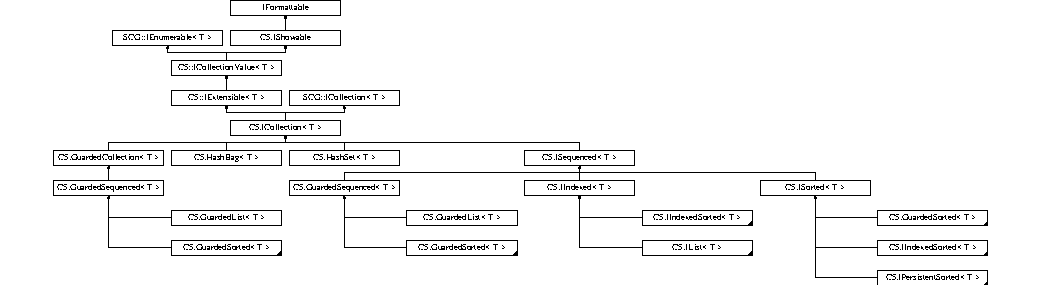
\includegraphics[height=3.825137cm]{interface_c5_1_1_i_collection}
\end{center}
\end{figure}
\subsection*{Public Member Functions}
\begin{DoxyCompactItemize}
\item 
new bool \hyperlink{interface_c5_1_1_i_collection_a525115f252ddca586fcbf1a0127be614}{Add} (T item)
\begin{DoxyCompactList}\small\item\em Add an item to this collection if possible. If this collection has set semantics, the item will be added if not already in the collection. If bag semantics, the item will always be added. \end{DoxyCompactList}\item 
new void \hyperlink{interface_c5_1_1_i_collection_aa2f928b7057eb84a1572307123e8239e}{Copy\+To} (T\mbox{[}$\,$\mbox{]} array, int index)
\begin{DoxyCompactList}\small\item\em Copy the items of this collection to a contiguous part of an array. \end{DoxyCompactList}\item 
int \hyperlink{interface_c5_1_1_i_collection_ae3a4fa01c3b09b9b372bb6f8639194ed}{Get\+Unsequenced\+Hash\+Code} ()
\begin{DoxyCompactList}\small\item\em The unordered collection hashcode is defined as the sum of \end{DoxyCompactList}\item 
bool \hyperlink{interface_c5_1_1_i_collection_a46fee76e3afed2b0510e94814ef832b2}{Unsequenced\+Equals} (\hyperlink{interface_c5_1_1_i_collection}{I\+Collection}$<$ T $>$ other\+Collection)
\begin{DoxyCompactList}\small\item\em Compare the contents of this collection to another one without regards to the sequence order. The comparison will use this collection\textquotesingle{}s itemequality\+Comparer to compare individual items. \end{DoxyCompactList}\item 
new bool \hyperlink{interface_c5_1_1_i_collection_a4de01b6d77ea5eaffccc8267b4454cdd}{Contains} (T item)
\begin{DoxyCompactList}\small\item\em Check if this collection contains (an item equivalent to according to the itemequality\+Comparer) a particular value. \end{DoxyCompactList}\item 
int \hyperlink{interface_c5_1_1_i_collection_acfe7e2c9b14c384762269edbb57b7fbe}{Contains\+Count} (T item)
\begin{DoxyCompactList}\small\item\em Count the number of items of the collection equal to a particular value. Returns 0 if and only if the value is not in the collection. \end{DoxyCompactList}\item 
\hyperlink{interface_c5_1_1_i_collection_value}{I\+Collection\+Value}$<$ T $>$ \hyperlink{interface_c5_1_1_i_collection_a074c4e1a90fb7f98c95834204352c28c}{Unique\+Items} ()
\item 
\hyperlink{interface_c5_1_1_i_collection_value}{I\+Collection\+Value}$<$ \hyperlink{struct_c5_1_1_key_value_pair}{Key\+Value\+Pair}$<$ T, int $>$ $>$ \hyperlink{interface_c5_1_1_i_collection_a623bd834b37b299c5f4948fdb6915fef}{Item\+Multiplicities} ()
\item 
bool \hyperlink{interface_c5_1_1_i_collection_a93abf02183a46f56af8d90f1d69982a8}{Contains\+All} (S\+C\+G.\+I\+Enumerable$<$ T $>$ items)
\begin{DoxyCompactList}\small\item\em Check whether this collection contains all the values in another collection. If this collection has bag semantics ( \end{DoxyCompactList}\item 
bool \hyperlink{interface_c5_1_1_i_collection_a96fd6cfd3df62e67922f9335b0fbbdcb}{Find} (ref T item)
\begin{DoxyCompactList}\small\item\em Check if this collection contains an item equivalent according to the itemequality\+Comparer to a particular value. If so, return in the ref argument (a binary copy of) the actual value found. \end{DoxyCompactList}\item 
bool \hyperlink{interface_c5_1_1_i_collection_a7f9e609ee1a7607596bb65aa5bdff303}{Find\+Or\+Add} (ref T item)
\begin{DoxyCompactList}\small\item\em Check if this collection contains an item equivalent according to the itemequality\+Comparer to a particular value. If so, return in the ref argument (a binary copy of) the actual value found. Else, add the item to the collection. \end{DoxyCompactList}\item 
bool \hyperlink{interface_c5_1_1_i_collection_acf060ba6b83289dc74bea61502318d56}{Update} (T item)
\begin{DoxyCompactList}\small\item\em Check if this collection contains an item equivalent according to the itemequality\+Comparer to a particular value. If so, update the item in the collection with a (binary copy of) the supplied value. If the collection has bag semantics, it depends on the value of Duplicates\+By\+Counting if this updates all equivalent copies in the collection or just one. \end{DoxyCompactList}\item 
bool \hyperlink{interface_c5_1_1_i_collection_ad1faa1738e02acf001aac16a3b948c78}{Update} (T item, out T olditem)
\begin{DoxyCompactList}\small\item\em Check if this collection contains an item equivalent according to the itemequality\+Comparer to a particular value. If so, update the item in the collection with a (binary copy of) the supplied value. If the collection has bag semantics, it depends on the value of Duplicates\+By\+Counting if this updates all equivalent copies in the collection or just one. \end{DoxyCompactList}\item 
bool \hyperlink{interface_c5_1_1_i_collection_a9739490d6271fb3a92221bca5da5e54b}{Update\+Or\+Add} (T item)
\begin{DoxyCompactList}\small\item\em Check if this collection contains an item equivalent according to the itemequality\+Comparer to a particular value. If so, update the item in the collection to with a binary copy of the supplied value; else add the value to the collection. \end{DoxyCompactList}\item 
bool \hyperlink{interface_c5_1_1_i_collection_a73a5d984e95e200de80261361bb7e57d}{Update\+Or\+Add} (T item, out T olditem)
\begin{DoxyCompactList}\small\item\em Check if this collection contains an item equivalent according to the itemequality\+Comparer to a particular value. If so, update the item in the collection to with a binary copy of the supplied value; else add the value to the collection. \end{DoxyCompactList}\item 
new bool \hyperlink{interface_c5_1_1_i_collection_ab4d6092ac09245ce46db91595fc1cdfe}{Remove} (T item)
\begin{DoxyCompactList}\small\item\em Remove a particular item from this collection. If the collection has bag semantics only one copy equivalent to the supplied item is removed. \end{DoxyCompactList}\item 
bool \hyperlink{interface_c5_1_1_i_collection_acbd124236c3f0958a8784d9c7c2dfd16}{Remove} (T item, out T removeditem)
\begin{DoxyCompactList}\small\item\em Remove a particular item from this collection if found. If the collection has bag semantics only one copy equivalent to the supplied item is removed, which one is implementation dependent. If an item was removed, report a binary copy of the actual item removed in the argument. \end{DoxyCompactList}\item 
void \hyperlink{interface_c5_1_1_i_collection_ad785b91be4edeb3fbe678db751f6355d}{Remove\+All\+Copies} (T item)
\begin{DoxyCompactList}\small\item\em Remove all items equivalent to a given value. \end{DoxyCompactList}\item 
void \hyperlink{interface_c5_1_1_i_collection_a9fb05163a1bd4b71bfd05101ff20c987}{Remove\+All} (S\+C\+G.\+I\+Enumerable$<$ T $>$ items)
\begin{DoxyCompactList}\small\item\em Remove all items in another collection from this one. If this collection has bag semantics, take multiplicities into account. \end{DoxyCompactList}\item 
new void \hyperlink{interface_c5_1_1_i_collection_abd83166ac00b3d36225d988fd4603e97}{Clear} ()
\begin{DoxyCompactList}\small\item\em Remove all items from this collection. \end{DoxyCompactList}\item 
void \hyperlink{interface_c5_1_1_i_collection_ac2672fb0557eeb24e328149c513c9a8b}{Retain\+All} (S\+C\+G.\+I\+Enumerable$<$ T $>$ items)
\begin{DoxyCompactList}\small\item\em Remove all items not in some other collection from this one. If this collection has bag semantics, take multiplicities into account. \end{DoxyCompactList}\end{DoxyCompactItemize}
\subsection*{Properties}
\begin{DoxyCompactItemize}
\item 
\hyperlink{namespace_c5_a615ba88dcdaa8d5a3c5f833a73d7fad6}{Speed} \hyperlink{interface_c5_1_1_i_collection_a0a9bcd98894c191206e18c7c20c3bdfe}{Contains\+Speed}\hspace{0.3cm}{\ttfamily  \mbox{[}get\mbox{]}}
\begin{DoxyCompactList}\small\item\em The value is symbolic indicating the type of asymptotic complexity in terms of the size of this collection (worst-\/case or amortized as relevant). \end{DoxyCompactList}\item 
new int \hyperlink{interface_c5_1_1_i_collection_abddff5406ccd4e98d8d96f41bf9d6d5b}{Count}\hspace{0.3cm}{\ttfamily  \mbox{[}get\mbox{]}}
\item 
new bool \hyperlink{interface_c5_1_1_i_collection_a94b0751f2b2fbd0519233b2755c055b4}{Is\+Read\+Only}\hspace{0.3cm}{\ttfamily  \mbox{[}get\mbox{]}}
\begin{DoxyCompactList}\small\item\em If true any call of an updating operation will throw an \end{DoxyCompactList}\end{DoxyCompactItemize}
\subsection*{Additional Inherited Members}


\subsection{Detailed Description}
The simplest interface of a main stream generic collection with lookup, insertion and removal operations. 



\subsection{Member Function Documentation}
\hypertarget{interface_c5_1_1_i_collection_a525115f252ddca586fcbf1a0127be614}{}\index{C5\+::\+I\+Collection@{C5\+::\+I\+Collection}!Add@{Add}}
\index{Add@{Add}!C5\+::\+I\+Collection@{C5\+::\+I\+Collection}}
\subsubsection[{Add(\+T item)}]{\setlength{\rightskip}{0pt plus 5cm}new bool {\bf C5.\+I\+Collection}$<$ T $>$.Add (
\begin{DoxyParamCaption}
\item[{T}]{item}
\end{DoxyParamCaption}
)}\label{interface_c5_1_1_i_collection_a525115f252ddca586fcbf1a0127be614}


Add an item to this collection if possible. If this collection has set semantics, the item will be added if not already in the collection. If bag semantics, the item will always be added. 


\begin{DoxyParams}{Parameters}
{\em item} & The item to add.\\
\hline
\end{DoxyParams}
\begin{DoxyReturn}{Returns}
True if item was added.
\end{DoxyReturn}


Implements \hyperlink{interface_c5_1_1_i_extensible_acfe8d39605927db1aff0572e2b5c1089}{C5.\+I\+Extensible$<$ T $>$}.



Implemented in \hyperlink{class_c5_1_1_hashed_linked_list_afcfc7b8da2f00ad7d8e3decadadd74bc}{C5.\+Hashed\+Linked\+List$<$ T $>$}, \hyperlink{class_c5_1_1_linked_list_ac205fdb2cfc336ee2c2843c04fcbad41}{C5.\+Linked\+List$<$ T $>$}, \hyperlink{class_c5_1_1_hashed_array_list_a4606087ab02e09f75ce6810b7a9d11a4}{C5.\+Hashed\+Array\+List$<$ T $>$}, \hyperlink{class_c5_1_1_array_list_a31f07a779aa64ee15f6875ab74682cb5}{C5.\+Array\+List$<$ T $>$}, \hyperlink{class_c5_1_1_sorted_array_a6d4091d5dd1ab9b4637ae16f2bca53e3}{C5.\+Sorted\+Array$<$ T $>$}, \hyperlink{class_c5_1_1_tree_bag_ac407a0824ba7e237c86525234b5b85bd}{C5.\+Tree\+Bag$<$ T $>$}, \hyperlink{class_c5_1_1_tree_set_ae2a3723eb4c1fabdb5b75d52d709f880}{C5.\+Tree\+Set$<$ T $>$}, \hyperlink{interface_c5_1_1_i_list_a800000d7344d000c1b8c67acda464a3d}{C5.\+I\+List$<$ T $>$}, \hyperlink{class_c5_1_1_guarded_collection_aa7fe8941b3b05d9e8622b830852cf12d}{C5.\+Guarded\+Collection$<$ T $>$}, \hyperlink{class_c5_1_1_hash_set_a0700ad4332214ac5d74f3a197bfd8774}{C5.\+Hash\+Set$<$ T $>$}, \hyperlink{class_c5_1_1_wrapped_array_a5be2e0d6422cbc8597e1bc7571b41048}{C5.\+Wrapped\+Array$<$ T $>$}, and \hyperlink{class_c5_1_1_hash_bag_a4cc47989ae0d25e5574558f973b85a8d}{C5.\+Hash\+Bag$<$ T $>$}.

\hypertarget{interface_c5_1_1_i_collection_abd83166ac00b3d36225d988fd4603e97}{}\index{C5\+::\+I\+Collection@{C5\+::\+I\+Collection}!Clear@{Clear}}
\index{Clear@{Clear}!C5\+::\+I\+Collection@{C5\+::\+I\+Collection}}
\subsubsection[{Clear()}]{\setlength{\rightskip}{0pt plus 5cm}new void {\bf C5.\+I\+Collection}$<$ T $>$.Clear (
\begin{DoxyParamCaption}
{}
\end{DoxyParamCaption}
)}\label{interface_c5_1_1_i_collection_abd83166ac00b3d36225d988fd4603e97}


Remove all items from this collection. 



Implemented in \hyperlink{class_c5_1_1_hashed_linked_list_a3d890e2da8746df9cf82d3ccaf561d44}{C5.\+Hashed\+Linked\+List$<$ T $>$}, \hyperlink{class_c5_1_1_linked_list_a936ee524a650660d23b62ff74ae306d9}{C5.\+Linked\+List$<$ T $>$}, \hyperlink{class_c5_1_1_tree_bag_a7e7ae58e999b8f2968b784df96d33695}{C5.\+Tree\+Bag$<$ T $>$}, \hyperlink{class_c5_1_1_hashed_array_list_aeca323e5f962607ee4384549aaba5d28}{C5.\+Hashed\+Array\+List$<$ T $>$}, \hyperlink{class_c5_1_1_tree_set_ae09b116f49bc00c9775c5799fd3a8ccf}{C5.\+Tree\+Set$<$ T $>$}, \hyperlink{class_c5_1_1_array_list_a1ed4a8838cc6a215101b6af156e7da08}{C5.\+Array\+List$<$ T $>$}, \hyperlink{interface_c5_1_1_i_list_aff6179e37b313d34596749484ae58ea4}{C5.\+I\+List$<$ T $>$}, \hyperlink{class_c5_1_1_sorted_array_ae316e2061d7224288fefe5cc3a848935}{C5.\+Sorted\+Array$<$ T $>$}, \hyperlink{class_c5_1_1_guarded_collection_ae26dd6085a063dd2b86d37b030b87750}{C5.\+Guarded\+Collection$<$ T $>$}, \hyperlink{class_c5_1_1_wrapped_array_aa57bfc8881b390314629e9830759eee5}{C5.\+Wrapped\+Array$<$ T $>$}, \hyperlink{class_c5_1_1_hash_set_a7bc97cd3a07e8e829c16e169ac71a075}{C5.\+Hash\+Set$<$ T $>$}, and \hyperlink{class_c5_1_1_hash_bag_a56b6eaa83ad0f3851cb48322f536f3d8}{C5.\+Hash\+Bag$<$ T $>$}.

\hypertarget{interface_c5_1_1_i_collection_a4de01b6d77ea5eaffccc8267b4454cdd}{}\index{C5\+::\+I\+Collection@{C5\+::\+I\+Collection}!Contains@{Contains}}
\index{Contains@{Contains}!C5\+::\+I\+Collection@{C5\+::\+I\+Collection}}
\subsubsection[{Contains(\+T item)}]{\setlength{\rightskip}{0pt plus 5cm}new bool {\bf C5.\+I\+Collection}$<$ T $>$.Contains (
\begin{DoxyParamCaption}
\item[{T}]{item}
\end{DoxyParamCaption}
)}\label{interface_c5_1_1_i_collection_a4de01b6d77ea5eaffccc8267b4454cdd}


Check if this collection contains (an item equivalent to according to the itemequality\+Comparer) a particular value. 


\begin{DoxyParams}{Parameters}
{\em item} & The value to check for.\\
\hline
\end{DoxyParams}
\begin{DoxyReturn}{Returns}
True if the items is in this collection.
\end{DoxyReturn}


Implemented in \hyperlink{class_c5_1_1_hashed_linked_list_a210cb416cd7418c59c89b99e2fce7bf8}{C5.\+Hashed\+Linked\+List$<$ T $>$}, \hyperlink{class_c5_1_1_linked_list_a9d3273641ee62248a93ed0eb58bed66a}{C5.\+Linked\+List$<$ T $>$}, \hyperlink{class_c5_1_1_hashed_array_list_a4b108299a930ceaecd8484023a656cf4}{C5.\+Hashed\+Array\+List$<$ T $>$}, \hyperlink{class_c5_1_1_array_list_a481c1d9104e4c5fbd4dd79be7a1e5c38}{C5.\+Array\+List$<$ T $>$}, \hyperlink{class_c5_1_1_tree_bag_ab3325de752c15c458b6c1359a2518e0a}{C5.\+Tree\+Bag$<$ T $>$}, \hyperlink{class_c5_1_1_tree_set_ac64161083bb695c31f6b459d4bd8c13e}{C5.\+Tree\+Set$<$ T $>$}, \hyperlink{class_c5_1_1_sorted_array_a3b50cf0032570c401d576f32104f68aa}{C5.\+Sorted\+Array$<$ T $>$}, \hyperlink{interface_c5_1_1_i_list_a108b607b042959d063e1ca77e242406c}{C5.\+I\+List$<$ T $>$}, \hyperlink{class_c5_1_1_guarded_collection_a1ffdf15a3e9daa80137e53fcd642770e}{C5.\+Guarded\+Collection$<$ T $>$}, \hyperlink{class_c5_1_1_wrapped_array_aeff3477a858a6f79b120be3ca1fd7c40}{C5.\+Wrapped\+Array$<$ T $>$}, \hyperlink{class_c5_1_1_hash_set_af664a08eff9d9941c43e043bf5b367c3}{C5.\+Hash\+Set$<$ T $>$}, and \hyperlink{class_c5_1_1_hash_bag_a4ab198cd099f684fc161c4055106c2a8}{C5.\+Hash\+Bag$<$ T $>$}.

\hypertarget{interface_c5_1_1_i_collection_a93abf02183a46f56af8d90f1d69982a8}{}\index{C5\+::\+I\+Collection@{C5\+::\+I\+Collection}!Contains\+All@{Contains\+All}}
\index{Contains\+All@{Contains\+All}!C5\+::\+I\+Collection@{C5\+::\+I\+Collection}}
\subsubsection[{Contains\+All(\+S\+C\+G.\+I\+Enumerable$<$ T $>$ items)}]{\setlength{\rightskip}{0pt plus 5cm}bool {\bf C5.\+I\+Collection}$<$ T $>$.Contains\+All (
\begin{DoxyParamCaption}
\item[{S\+C\+G.\+I\+Enumerable$<$ T $>$}]{items}
\end{DoxyParamCaption}
)}\label{interface_c5_1_1_i_collection_a93abf02183a46f56af8d90f1d69982a8}


Check whether this collection contains all the values in another collection. If this collection has bag semantics ( 

{\ttfamily Allows\+Duplicates==true}) the check is made with respect to multiplicities, else multiplicities are not taken into account. 


\begin{DoxyParams}{Parameters}
{\em items} & The \\
\hline
\end{DoxyParams}
\begin{DoxyReturn}{Returns}
True if all values in 
\begin{DoxyCode}
items
\end{DoxyCode}
is in this collection.
\end{DoxyReturn}


Implemented in \hyperlink{class_c5_1_1_hashed_linked_list_a8592fd2f2b3cea5329acaf4331dff7bc}{C5.\+Hashed\+Linked\+List$<$ T $>$}, \hyperlink{class_c5_1_1_linked_list_a10a876c3bb88997efbca9d7ab6cc9ed4}{C5.\+Linked\+List$<$ T $>$}, \hyperlink{class_c5_1_1_tree_bag_ada5a4e4666a76bb810a722cea086e336}{C5.\+Tree\+Bag$<$ T $>$}, \hyperlink{class_c5_1_1_hashed_array_list_ae3145f69b175e6b3d9af471b3ef89c80}{C5.\+Hashed\+Array\+List$<$ T $>$}, \hyperlink{class_c5_1_1_tree_set_a89f60df47bcd103257f38983d1ae11e3}{C5.\+Tree\+Set$<$ T $>$}, \hyperlink{class_c5_1_1_array_list_a59f882585e714af67e2ba7211e3d3595}{C5.\+Array\+List$<$ T $>$}, \hyperlink{class_c5_1_1_sorted_array_a5112ec4af3590219c5b24957f9a0dad9}{C5.\+Sorted\+Array$<$ T $>$}, \hyperlink{class_c5_1_1_guarded_collection_a57f6d96d3787483e45837b2700d9459b}{C5.\+Guarded\+Collection$<$ T $>$}, \hyperlink{class_c5_1_1_hash_set_ad7c29ad00f9697d4a07e03986c84770e}{C5.\+Hash\+Set$<$ T $>$}, \hyperlink{class_c5_1_1_wrapped_array_a2e1371765df8e9ecc8f928129ddd523f}{C5.\+Wrapped\+Array$<$ T $>$}, and \hyperlink{class_c5_1_1_hash_bag_aff78f22f0c5e6b5dc2c550cd0d5a24e3}{C5.\+Hash\+Bag$<$ T $>$}.

\hypertarget{interface_c5_1_1_i_collection_acfe7e2c9b14c384762269edbb57b7fbe}{}\index{C5\+::\+I\+Collection@{C5\+::\+I\+Collection}!Contains\+Count@{Contains\+Count}}
\index{Contains\+Count@{Contains\+Count}!C5\+::\+I\+Collection@{C5\+::\+I\+Collection}}
\subsubsection[{Contains\+Count(\+T item)}]{\setlength{\rightskip}{0pt plus 5cm}int {\bf C5.\+I\+Collection}$<$ T $>$.Contains\+Count (
\begin{DoxyParamCaption}
\item[{T}]{item}
\end{DoxyParamCaption}
)}\label{interface_c5_1_1_i_collection_acfe7e2c9b14c384762269edbb57b7fbe}


Count the number of items of the collection equal to a particular value. Returns 0 if and only if the value is not in the collection. 


\begin{DoxyParams}{Parameters}
{\em item} & The value to count.\\
\hline
\end{DoxyParams}
\begin{DoxyReturn}{Returns}
The number of copies found.
\end{DoxyReturn}


Implemented in \hyperlink{class_c5_1_1_hashed_linked_list_a0bf0f2c26ac2975f17d240880ca79de5}{C5.\+Hashed\+Linked\+List$<$ T $>$}, \hyperlink{class_c5_1_1_linked_list_a7ea7467fd1107ed2d38e29966f188266}{C5.\+Linked\+List$<$ T $>$}, \hyperlink{class_c5_1_1_tree_bag_a3a7a0f7538cd89da7e9b10e3311bd521}{C5.\+Tree\+Bag$<$ T $>$}, \hyperlink{class_c5_1_1_tree_set_ab2df8bca715b6d3d24263e42dd4df84d}{C5.\+Tree\+Set$<$ T $>$}, \hyperlink{class_c5_1_1_hashed_array_list_a4fb06172f38039104765ee9d6ed78842}{C5.\+Hashed\+Array\+List$<$ T $>$}, \hyperlink{class_c5_1_1_array_list_a64988ea7ea5325a0ee85d96ed32401dd}{C5.\+Array\+List$<$ T $>$}, \hyperlink{class_c5_1_1_sorted_array_aa8ebd1f6cb041cf1d57299f217f65243}{C5.\+Sorted\+Array$<$ T $>$}, \hyperlink{class_c5_1_1_hash_set_a6ae7c12192030c64a6268546bdb21fbe}{C5.\+Hash\+Set$<$ T $>$}, \hyperlink{class_c5_1_1_guarded_collection_ae5bfa7d92d0ebe7d185f04f8836685c7}{C5.\+Guarded\+Collection$<$ T $>$}, \hyperlink{class_c5_1_1_hash_bag_ae9d24cf11e28837e35dfcf9a89858a90}{C5.\+Hash\+Bag$<$ T $>$}, and \hyperlink{class_c5_1_1_wrapped_array_a9d839f2be462e1dbda9ed69fe15a532f}{C5.\+Wrapped\+Array$<$ T $>$}.

\hypertarget{interface_c5_1_1_i_collection_aa2f928b7057eb84a1572307123e8239e}{}\index{C5\+::\+I\+Collection@{C5\+::\+I\+Collection}!Copy\+To@{Copy\+To}}
\index{Copy\+To@{Copy\+To}!C5\+::\+I\+Collection@{C5\+::\+I\+Collection}}
\subsubsection[{Copy\+To(\+T[] array, int index)}]{\setlength{\rightskip}{0pt plus 5cm}new void {\bf C5.\+I\+Collection}$<$ T $>$.Copy\+To (
\begin{DoxyParamCaption}
\item[{T\mbox{[}$\,$\mbox{]}}]{array, }
\item[{int}]{index}
\end{DoxyParamCaption}
)}\label{interface_c5_1_1_i_collection_aa2f928b7057eb84a1572307123e8239e}


Copy the items of this collection to a contiguous part of an array. 


\begin{DoxyParams}{Parameters}
{\em array} & The array to copy to\\
\hline
{\em index} & The index at which to copy the first item\\
\hline
\end{DoxyParams}


Implements \hyperlink{interface_c5_1_1_i_collection_value_aced299d8dce69c33ff75b598e39581d1}{C5.\+I\+Collection\+Value$<$ T $>$}.



Implemented in \hyperlink{interface_c5_1_1_i_list_a6fef986271bdc88a6f38cb15bd15690f}{C5.\+I\+List$<$ T $>$}, \hyperlink{class_c5_1_1_wrapped_array_a3dfd50eb13f5b3f90445e217214fae96}{C5.\+Wrapped\+Array$<$ T $>$}, and \hyperlink{class_c5_1_1_hash_bag_ad7ffdb5c882c290aa8b398d499a9d2ac}{C5.\+Hash\+Bag$<$ T $>$}.

\hypertarget{interface_c5_1_1_i_collection_a96fd6cfd3df62e67922f9335b0fbbdcb}{}\index{C5\+::\+I\+Collection@{C5\+::\+I\+Collection}!Find@{Find}}
\index{Find@{Find}!C5\+::\+I\+Collection@{C5\+::\+I\+Collection}}
\subsubsection[{Find(ref T item)}]{\setlength{\rightskip}{0pt plus 5cm}bool {\bf C5.\+I\+Collection}$<$ T $>$.Find (
\begin{DoxyParamCaption}
\item[{ref T}]{item}
\end{DoxyParamCaption}
)}\label{interface_c5_1_1_i_collection_a96fd6cfd3df62e67922f9335b0fbbdcb}


Check if this collection contains an item equivalent according to the itemequality\+Comparer to a particular value. If so, return in the ref argument (a binary copy of) the actual value found. 


\begin{DoxyParams}{Parameters}
{\em item} & The value to look for.\\
\hline
\end{DoxyParams}
\begin{DoxyReturn}{Returns}
True if the items is in this collection.
\end{DoxyReturn}


Implemented in \hyperlink{class_c5_1_1_hashed_linked_list_a71b0404288670bcd57700dafe8f9933c}{C5.\+Hashed\+Linked\+List$<$ T $>$}, \hyperlink{class_c5_1_1_linked_list_a04291749c18af8f2f9e9f943f7ccc91d}{C5.\+Linked\+List$<$ T $>$}, \hyperlink{class_c5_1_1_hashed_array_list_ac29e24d17686e2c3998a590a60b27d71}{C5.\+Hashed\+Array\+List$<$ T $>$}, \hyperlink{class_c5_1_1_array_list_a835191c794936ab62f751aaef835254d}{C5.\+Array\+List$<$ T $>$}, \hyperlink{class_c5_1_1_tree_bag_a9d195da9dc0c1ccc78c72f1d99b969e6}{C5.\+Tree\+Bag$<$ T $>$}, \hyperlink{class_c5_1_1_tree_set_a6c2fb30b79c7a0a7212804503c0db97e}{C5.\+Tree\+Set$<$ T $>$}, \hyperlink{class_c5_1_1_sorted_array_afa6a8770273981e3641d7d13edd0f39b}{C5.\+Sorted\+Array$<$ T $>$}, \hyperlink{class_c5_1_1_guarded_collection_ab447aa674e79536b0c92f7010101ce89}{C5.\+Guarded\+Collection$<$ T $>$}, \hyperlink{class_c5_1_1_wrapped_array_ad8903faa6514226fa26155c9e2f757b2}{C5.\+Wrapped\+Array$<$ T $>$}, \hyperlink{class_c5_1_1_hash_set_a68b40c2f8c5483825915945d0f21278a}{C5.\+Hash\+Set$<$ T $>$}, and \hyperlink{class_c5_1_1_hash_bag_a596f1c7fdcc7867d3b93ffb18f106655}{C5.\+Hash\+Bag$<$ T $>$}.

\hypertarget{interface_c5_1_1_i_collection_a7f9e609ee1a7607596bb65aa5bdff303}{}\index{C5\+::\+I\+Collection@{C5\+::\+I\+Collection}!Find\+Or\+Add@{Find\+Or\+Add}}
\index{Find\+Or\+Add@{Find\+Or\+Add}!C5\+::\+I\+Collection@{C5\+::\+I\+Collection}}
\subsubsection[{Find\+Or\+Add(ref T item)}]{\setlength{\rightskip}{0pt plus 5cm}bool {\bf C5.\+I\+Collection}$<$ T $>$.Find\+Or\+Add (
\begin{DoxyParamCaption}
\item[{ref T}]{item}
\end{DoxyParamCaption}
)}\label{interface_c5_1_1_i_collection_a7f9e609ee1a7607596bb65aa5bdff303}


Check if this collection contains an item equivalent according to the itemequality\+Comparer to a particular value. If so, return in the ref argument (a binary copy of) the actual value found. Else, add the item to the collection. 


\begin{DoxyParams}{Parameters}
{\em item} & The value to look for.\\
\hline
\end{DoxyParams}
\begin{DoxyReturn}{Returns}
True if the item was found (hence not added).
\end{DoxyReturn}


Implemented in \hyperlink{class_c5_1_1_hashed_linked_list_a71a1257a1ba4328713fb87daa3b45675}{C5.\+Hashed\+Linked\+List$<$ T $>$}, \hyperlink{class_c5_1_1_linked_list_ae6d34353ca7075c45dbac47a8d79dceb}{C5.\+Linked\+List$<$ T $>$}, \hyperlink{class_c5_1_1_hashed_array_list_a7adaad90a9e57a90c3bc197dc4d1289c}{C5.\+Hashed\+Array\+List$<$ T $>$}, \hyperlink{class_c5_1_1_array_list_a35b8836d9228034409fc10e4dc5d7779}{C5.\+Array\+List$<$ T $>$}, \hyperlink{class_c5_1_1_tree_bag_a8c43b82821162894db0fc7aa18e7ee6a}{C5.\+Tree\+Bag$<$ T $>$}, \hyperlink{class_c5_1_1_tree_set_ae73144d09bef526e903714cd013fedb6}{C5.\+Tree\+Set$<$ T $>$}, \hyperlink{class_c5_1_1_sorted_array_ac7f5931e6681c9bfe5a1dabb9a326c8e}{C5.\+Sorted\+Array$<$ T $>$}, \hyperlink{class_c5_1_1_guarded_collection_a06f9fdffc49fe7e5d618366b749fe8be}{C5.\+Guarded\+Collection$<$ T $>$}, \hyperlink{class_c5_1_1_wrapped_array_afe18ba420f983ab2a011cde8bda43cd5}{C5.\+Wrapped\+Array$<$ T $>$}, \hyperlink{class_c5_1_1_hash_set_a0b1d42cbbc91e630ab0917a2b17e8ca1}{C5.\+Hash\+Set$<$ T $>$}, and \hyperlink{class_c5_1_1_hash_bag_afc84f71f4abef8b7a96f8b5d9153a270}{C5.\+Hash\+Bag$<$ T $>$}.

\hypertarget{interface_c5_1_1_i_collection_ae3a4fa01c3b09b9b372bb6f8639194ed}{}\index{C5\+::\+I\+Collection@{C5\+::\+I\+Collection}!Get\+Unsequenced\+Hash\+Code@{Get\+Unsequenced\+Hash\+Code}}
\index{Get\+Unsequenced\+Hash\+Code@{Get\+Unsequenced\+Hash\+Code}!C5\+::\+I\+Collection@{C5\+::\+I\+Collection}}
\subsubsection[{Get\+Unsequenced\+Hash\+Code()}]{\setlength{\rightskip}{0pt plus 5cm}int {\bf C5.\+I\+Collection}$<$ T $>$.Get\+Unsequenced\+Hash\+Code (
\begin{DoxyParamCaption}
{}
\end{DoxyParamCaption}
)}\label{interface_c5_1_1_i_collection_ae3a4fa01c3b09b9b372bb6f8639194ed}


The unordered collection hashcode is defined as the sum of 

{\ttfamily h(hashcode(item))} over the items of the collection, where the function {\ttfamily h} is a function from int to int of the form {\ttfamily  t -\/$>$ (a0$\ast$t+b0)$^\wedge$(a1$\ast$t+b1)$^\wedge$(a2$\ast$t+b2)}, where the ax and bx are the same for all collection classes. 

The current implementation uses fixed values for the ax and bx, specified as constants in the code.

\begin{DoxyReturn}{Returns}
The unordered hashcode of this collection.
\end{DoxyReturn}


Implemented in \hyperlink{class_c5_1_1_hashed_linked_list_afa9c20b419017663841ffd613d31e75b}{C5.\+Hashed\+Linked\+List$<$ T $>$}, \hyperlink{class_c5_1_1_linked_list_a66dd343eb1edfd17074b200fccd59621}{C5.\+Linked\+List$<$ T $>$}, \hyperlink{class_c5_1_1_hashed_array_list_a8f23bbdc50d2c951e19fad0008f2f25a}{C5.\+Hashed\+Array\+List$<$ T $>$}, \hyperlink{class_c5_1_1_array_list_a4f75d053012574e34e670597aa392e6f}{C5.\+Array\+List$<$ T $>$}, \hyperlink{class_c5_1_1_guarded_collection_a993f9bfefdd11d4bf8f776215db02c31}{C5.\+Guarded\+Collection$<$ T $>$}, and \hyperlink{class_c5_1_1_wrapped_array_a9e66ede7a619e13da4307ec6c8df6c0d}{C5.\+Wrapped\+Array$<$ T $>$}.

\hypertarget{interface_c5_1_1_i_collection_a623bd834b37b299c5f4948fdb6915fef}{}\index{C5\+::\+I\+Collection@{C5\+::\+I\+Collection}!Item\+Multiplicities@{Item\+Multiplicities}}
\index{Item\+Multiplicities@{Item\+Multiplicities}!C5\+::\+I\+Collection@{C5\+::\+I\+Collection}}
\subsubsection[{Item\+Multiplicities()}]{\setlength{\rightskip}{0pt plus 5cm}{\bf I\+Collection\+Value}$<${\bf Key\+Value\+Pair}$<$T, int$>$ $>$ {\bf C5.\+I\+Collection}$<$ T $>$.Item\+Multiplicities (
\begin{DoxyParamCaption}
{}
\end{DoxyParamCaption}
)}\label{interface_c5_1_1_i_collection_a623bd834b37b299c5f4948fdb6915fef}




\begin{DoxyReturn}{Returns}

\end{DoxyReturn}


Implemented in \hyperlink{class_c5_1_1_hashed_linked_list_a0cee8e4c1768986a4d167f34c8a3c227}{C5.\+Hashed\+Linked\+List$<$ T $>$}, \hyperlink{class_c5_1_1_linked_list_a385ed37a08dddfbef49633940710adf0}{C5.\+Linked\+List$<$ T $>$}, \hyperlink{class_c5_1_1_tree_bag_a9a6a1f53ff0b1874f1936c960319f3ab}{C5.\+Tree\+Bag$<$ T $>$}, \hyperlink{class_c5_1_1_tree_set_a34003354cd733efb85aa9bf871b2cd71}{C5.\+Tree\+Set$<$ T $>$}, \hyperlink{class_c5_1_1_hashed_array_list_a8a36b62fa880e713de8e5d8ccfd19595}{C5.\+Hashed\+Array\+List$<$ T $>$}, \hyperlink{class_c5_1_1_array_list_a335c5003a3607d44e571f7fa444e75cb}{C5.\+Array\+List$<$ T $>$}, \hyperlink{class_c5_1_1_sorted_array_af410b4ad3cee1526a8d3b4fc6ec7a3c5}{C5.\+Sorted\+Array$<$ T $>$}, \hyperlink{class_c5_1_1_hash_set_ae8e2ee2134a81967efe6fef79d67a0fc}{C5.\+Hash\+Set$<$ T $>$}, \hyperlink{class_c5_1_1_guarded_collection_ad400f5862b15a3a0c59a4cb7d347f926}{C5.\+Guarded\+Collection$<$ T $>$}, \hyperlink{class_c5_1_1_hash_bag_a25efbcb614ab06216f52a7f34f74f8fc}{C5.\+Hash\+Bag$<$ T $>$}, and \hyperlink{class_c5_1_1_wrapped_array_a71341ae57222c7e5d5f16b96b91ccf81}{C5.\+Wrapped\+Array$<$ T $>$}.

\hypertarget{interface_c5_1_1_i_collection_ab4d6092ac09245ce46db91595fc1cdfe}{}\index{C5\+::\+I\+Collection@{C5\+::\+I\+Collection}!Remove@{Remove}}
\index{Remove@{Remove}!C5\+::\+I\+Collection@{C5\+::\+I\+Collection}}
\subsubsection[{Remove(\+T item)}]{\setlength{\rightskip}{0pt plus 5cm}new bool {\bf C5.\+I\+Collection}$<$ T $>$.Remove (
\begin{DoxyParamCaption}
\item[{T}]{item}
\end{DoxyParamCaption}
)}\label{interface_c5_1_1_i_collection_ab4d6092ac09245ce46db91595fc1cdfe}


Remove a particular item from this collection. If the collection has bag semantics only one copy equivalent to the supplied item is removed. 


\begin{DoxyParams}{Parameters}
{\em item} & The value to remove.\\
\hline
\end{DoxyParams}
\begin{DoxyReturn}{Returns}
True if the item was found (and removed).
\end{DoxyReturn}


Implemented in \hyperlink{class_c5_1_1_hashed_linked_list_ad97f128fe00bf12c8e77678f08bd27e1}{C5.\+Hashed\+Linked\+List$<$ T $>$}, \hyperlink{class_c5_1_1_linked_list_a16561b02cc72e8d8191c32a84af13d81}{C5.\+Linked\+List$<$ T $>$}, \hyperlink{class_c5_1_1_hashed_array_list_a4453b3955bce1670914b4aa2f469b4c0}{C5.\+Hashed\+Array\+List$<$ T $>$}, \hyperlink{class_c5_1_1_array_list_a8e3d348ba6d557785028bee0b9a25bf8}{C5.\+Array\+List$<$ T $>$}, \hyperlink{class_c5_1_1_tree_bag_ac12beb566f28e1e8091a2db06721d43d}{C5.\+Tree\+Bag$<$ T $>$}, \hyperlink{class_c5_1_1_tree_set_acc2195583c6e6b20ebe2fba3837ac103}{C5.\+Tree\+Set$<$ T $>$}, \hyperlink{class_c5_1_1_sorted_array_a4bd50348d1eaf888c4c66b46dcf52d04}{C5.\+Sorted\+Array$<$ T $>$}, \hyperlink{interface_c5_1_1_i_list_a14dd6b1e7f06807dc6a45edf0f83dfbd}{C5.\+I\+List$<$ T $>$}, \hyperlink{class_c5_1_1_guarded_collection_a5228eac1c6eb5341b2ab20a3095fa066}{C5.\+Guarded\+Collection$<$ T $>$}, \hyperlink{class_c5_1_1_wrapped_array_a3f312170b262e9f56b4d23442eb98029}{C5.\+Wrapped\+Array$<$ T $>$}, \hyperlink{class_c5_1_1_hash_set_ac9b5cd955239472a848788ce53345853}{C5.\+Hash\+Set$<$ T $>$}, and \hyperlink{class_c5_1_1_hash_bag_aecff446396494ee3d10ee53f5bc78ce5}{C5.\+Hash\+Bag$<$ T $>$}.

\hypertarget{interface_c5_1_1_i_collection_acbd124236c3f0958a8784d9c7c2dfd16}{}\index{C5\+::\+I\+Collection@{C5\+::\+I\+Collection}!Remove@{Remove}}
\index{Remove@{Remove}!C5\+::\+I\+Collection@{C5\+::\+I\+Collection}}
\subsubsection[{Remove(\+T item, out T removeditem)}]{\setlength{\rightskip}{0pt plus 5cm}bool {\bf C5.\+I\+Collection}$<$ T $>$.Remove (
\begin{DoxyParamCaption}
\item[{T}]{item, }
\item[{out T}]{removeditem}
\end{DoxyParamCaption}
)}\label{interface_c5_1_1_i_collection_acbd124236c3f0958a8784d9c7c2dfd16}


Remove a particular item from this collection if found. If the collection has bag semantics only one copy equivalent to the supplied item is removed, which one is implementation dependent. If an item was removed, report a binary copy of the actual item removed in the argument. 


\begin{DoxyParams}{Parameters}
{\em item} & The value to remove.\\
\hline
{\em removeditem} & The value removed if any.\\
\hline
\end{DoxyParams}
\begin{DoxyReturn}{Returns}
True if the item was found (and removed).
\end{DoxyReturn}


Implemented in \hyperlink{class_c5_1_1_hashed_linked_list_ab1348cf4b0e02e147f6dd08a539e2c61}{C5.\+Hashed\+Linked\+List$<$ T $>$}, \hyperlink{class_c5_1_1_linked_list_a37bbd34f4ba9f1771ebd0854f1b5037a}{C5.\+Linked\+List$<$ T $>$}, \hyperlink{class_c5_1_1_hashed_array_list_aaf108802a6f4024858b9d178109126ee}{C5.\+Hashed\+Array\+List$<$ T $>$}, \hyperlink{class_c5_1_1_array_list_adc146d07d67bf7e96f07fb604c83b2c9}{C5.\+Array\+List$<$ T $>$}, \hyperlink{class_c5_1_1_tree_bag_a0e0865e018b7ddae7c0fefb85df150e6}{C5.\+Tree\+Bag$<$ T $>$}, \hyperlink{class_c5_1_1_tree_set_aa4e7e4d3479ebd289308ba8f9c239bad}{C5.\+Tree\+Set$<$ T $>$}, \hyperlink{class_c5_1_1_sorted_array_a02f963bfc980a73d45ff434fa4d8eae7}{C5.\+Sorted\+Array$<$ T $>$}, \hyperlink{class_c5_1_1_guarded_collection_afa3304903fb8b724e52bb6cc4f12e6a9}{C5.\+Guarded\+Collection$<$ T $>$}, \hyperlink{class_c5_1_1_wrapped_array_aeb6273eab4c6798ab5ae3f7d1b64dff1}{C5.\+Wrapped\+Array$<$ T $>$}, \hyperlink{class_c5_1_1_hash_set_a7e97b49057ee44abddb8fbd83b56b78a}{C5.\+Hash\+Set$<$ T $>$}, and \hyperlink{class_c5_1_1_hash_bag_a15514e59b510fc1e5d1d4b5bc3ca16c8}{C5.\+Hash\+Bag$<$ T $>$}.

\hypertarget{interface_c5_1_1_i_collection_a9fb05163a1bd4b71bfd05101ff20c987}{}\index{C5\+::\+I\+Collection@{C5\+::\+I\+Collection}!Remove\+All@{Remove\+All}}
\index{Remove\+All@{Remove\+All}!C5\+::\+I\+Collection@{C5\+::\+I\+Collection}}
\subsubsection[{Remove\+All(\+S\+C\+G.\+I\+Enumerable$<$ T $>$ items)}]{\setlength{\rightskip}{0pt plus 5cm}void {\bf C5.\+I\+Collection}$<$ T $>$.Remove\+All (
\begin{DoxyParamCaption}
\item[{S\+C\+G.\+I\+Enumerable$<$ T $>$}]{items}
\end{DoxyParamCaption}
)}\label{interface_c5_1_1_i_collection_a9fb05163a1bd4b71bfd05101ff20c987}


Remove all items in another collection from this one. If this collection has bag semantics, take multiplicities into account. 


\begin{DoxyParams}{Parameters}
{\em items} & The items to remove.\\
\hline
\end{DoxyParams}


Implemented in \hyperlink{class_c5_1_1_hashed_linked_list_a13f0ec0b64eaba0412a48e8df37ba210}{C5.\+Hashed\+Linked\+List$<$ T $>$}, \hyperlink{class_c5_1_1_linked_list_a9f346a6bf713cae5170ee71e662918cc}{C5.\+Linked\+List$<$ T $>$}, \hyperlink{class_c5_1_1_tree_bag_a2e37aa0e335a6b94842841e692b3f59a}{C5.\+Tree\+Bag$<$ T $>$}, \hyperlink{class_c5_1_1_tree_set_aab27d3466268b7943b82c28d33dd1579}{C5.\+Tree\+Set$<$ T $>$}, \hyperlink{class_c5_1_1_hashed_array_list_a9598f605bb5e2de9f4a1bfce80a0dd0b}{C5.\+Hashed\+Array\+List$<$ T $>$}, \hyperlink{class_c5_1_1_array_list_aaa0409bfe3256b9e5749ff8710f89b45}{C5.\+Array\+List$<$ T $>$}, \hyperlink{class_c5_1_1_sorted_array_aedd7008a07388c8ad0463f52e3f2562c}{C5.\+Sorted\+Array$<$ T $>$}, \hyperlink{class_c5_1_1_guarded_collection_ab5e36593deb380b90bb35f7a283e48fc}{C5.\+Guarded\+Collection$<$ T $>$}, \hyperlink{class_c5_1_1_wrapped_array_a87989abbf2d41125036606805dcdd926}{C5.\+Wrapped\+Array$<$ T $>$}, \hyperlink{class_c5_1_1_hash_set_afc71edbb94b37e74b25d0d489c36dc3b}{C5.\+Hash\+Set$<$ T $>$}, and \hyperlink{class_c5_1_1_hash_bag_ab207da94ab560f22eabefaa17fdbd6d7}{C5.\+Hash\+Bag$<$ T $>$}.

\hypertarget{interface_c5_1_1_i_collection_ad785b91be4edeb3fbe678db751f6355d}{}\index{C5\+::\+I\+Collection@{C5\+::\+I\+Collection}!Remove\+All\+Copies@{Remove\+All\+Copies}}
\index{Remove\+All\+Copies@{Remove\+All\+Copies}!C5\+::\+I\+Collection@{C5\+::\+I\+Collection}}
\subsubsection[{Remove\+All\+Copies(\+T item)}]{\setlength{\rightskip}{0pt plus 5cm}void {\bf C5.\+I\+Collection}$<$ T $>$.Remove\+All\+Copies (
\begin{DoxyParamCaption}
\item[{T}]{item}
\end{DoxyParamCaption}
)}\label{interface_c5_1_1_i_collection_ad785b91be4edeb3fbe678db751f6355d}


Remove all items equivalent to a given value. 


\begin{DoxyParams}{Parameters}
{\em item} & The value to remove.\\
\hline
\end{DoxyParams}


Implemented in \hyperlink{class_c5_1_1_hashed_linked_list_ad3b535da6c6624412c450c96560d2f51}{C5.\+Hashed\+Linked\+List$<$ T $>$}, \hyperlink{class_c5_1_1_linked_list_a307f85230fbf4f94a444743220080030}{C5.\+Linked\+List$<$ T $>$}, \hyperlink{class_c5_1_1_tree_bag_a9fd092cffe3ba3dba034ca1453a75819}{C5.\+Tree\+Bag$<$ T $>$}, \hyperlink{class_c5_1_1_tree_set_a6ffcb62b0139bd09d755103b26ea4c9b}{C5.\+Tree\+Set$<$ T $>$}, \hyperlink{class_c5_1_1_hashed_array_list_a5b7779ece9c62551eb1c1a24c53906a5}{C5.\+Hashed\+Array\+List$<$ T $>$}, \hyperlink{class_c5_1_1_array_list_a375c1c5bb0d8b80208b32f90128f7347}{C5.\+Array\+List$<$ T $>$}, \hyperlink{class_c5_1_1_sorted_array_a7f3181ddc47e86407b2c87d593dc8386}{C5.\+Sorted\+Array$<$ T $>$}, \hyperlink{class_c5_1_1_guarded_collection_a912c6184ee4b074c3981f9dde491a94b}{C5.\+Guarded\+Collection$<$ T $>$}, \hyperlink{class_c5_1_1_hash_set_a07eacbcc5850774881dd596676e6b134}{C5.\+Hash\+Set$<$ T $>$}, \hyperlink{class_c5_1_1_wrapped_array_af733180804bf7ee5a4a0ece7f6cb12c3}{C5.\+Wrapped\+Array$<$ T $>$}, and \hyperlink{class_c5_1_1_hash_bag_ac7e182e2105701436c1288feaeeef627}{C5.\+Hash\+Bag$<$ T $>$}.

\hypertarget{interface_c5_1_1_i_collection_ac2672fb0557eeb24e328149c513c9a8b}{}\index{C5\+::\+I\+Collection@{C5\+::\+I\+Collection}!Retain\+All@{Retain\+All}}
\index{Retain\+All@{Retain\+All}!C5\+::\+I\+Collection@{C5\+::\+I\+Collection}}
\subsubsection[{Retain\+All(\+S\+C\+G.\+I\+Enumerable$<$ T $>$ items)}]{\setlength{\rightskip}{0pt plus 5cm}void {\bf C5.\+I\+Collection}$<$ T $>$.Retain\+All (
\begin{DoxyParamCaption}
\item[{S\+C\+G.\+I\+Enumerable$<$ T $>$}]{items}
\end{DoxyParamCaption}
)}\label{interface_c5_1_1_i_collection_ac2672fb0557eeb24e328149c513c9a8b}


Remove all items not in some other collection from this one. If this collection has bag semantics, take multiplicities into account. 


\begin{DoxyParams}{Parameters}
{\em items} & The items to retain.\\
\hline
\end{DoxyParams}


Implemented in \hyperlink{class_c5_1_1_hashed_linked_list_a56ae0d7eee62da4832bfc2363adf056e}{C5.\+Hashed\+Linked\+List$<$ T $>$}, \hyperlink{class_c5_1_1_linked_list_af59cb7a4dbffd061ffc577a34021db1c}{C5.\+Linked\+List$<$ T $>$}, \hyperlink{class_c5_1_1_tree_bag_a5e94ab2d0e81d3834d60824482a5568c}{C5.\+Tree\+Bag$<$ T $>$}, \hyperlink{class_c5_1_1_tree_set_aecd559b74434fcf369cd55fa0235f6e8}{C5.\+Tree\+Set$<$ T $>$}, \hyperlink{class_c5_1_1_hashed_array_list_a2c474cfc8e742163eec9bfba91169a79}{C5.\+Hashed\+Array\+List$<$ T $>$}, \hyperlink{class_c5_1_1_array_list_a7f3f5674779507d03f9139dea24977a2}{C5.\+Array\+List$<$ T $>$}, \hyperlink{class_c5_1_1_sorted_array_abb280e148baa50e5793aa4368ce33876}{C5.\+Sorted\+Array$<$ T $>$}, \hyperlink{class_c5_1_1_guarded_collection_addd89e0bb9db15b64f24d64b7720761d}{C5.\+Guarded\+Collection$<$ T $>$}, \hyperlink{class_c5_1_1_wrapped_array_aca9b3686c472517405451a8342da0de1}{C5.\+Wrapped\+Array$<$ T $>$}, \hyperlink{class_c5_1_1_hash_set_a5ab8110d40df588e0214b2d55eb085ce}{C5.\+Hash\+Set$<$ T $>$}, and \hyperlink{class_c5_1_1_hash_bag_aa83a436a144bb83ea23059d2b9d54a45}{C5.\+Hash\+Bag$<$ T $>$}.

\hypertarget{interface_c5_1_1_i_collection_a074c4e1a90fb7f98c95834204352c28c}{}\index{C5\+::\+I\+Collection@{C5\+::\+I\+Collection}!Unique\+Items@{Unique\+Items}}
\index{Unique\+Items@{Unique\+Items}!C5\+::\+I\+Collection@{C5\+::\+I\+Collection}}
\subsubsection[{Unique\+Items()}]{\setlength{\rightskip}{0pt plus 5cm}{\bf I\+Collection\+Value}$<$T$>$ {\bf C5.\+I\+Collection}$<$ T $>$.Unique\+Items (
\begin{DoxyParamCaption}
{}
\end{DoxyParamCaption}
)}\label{interface_c5_1_1_i_collection_a074c4e1a90fb7f98c95834204352c28c}




\begin{DoxyReturn}{Returns}

\end{DoxyReturn}


Implemented in \hyperlink{class_c5_1_1_hashed_linked_list_a11f80f9fc36538f944da608ce8ae8e6e}{C5.\+Hashed\+Linked\+List$<$ T $>$}, \hyperlink{class_c5_1_1_linked_list_ae1fa3b103e84b621d2746bdf73e5dec5}{C5.\+Linked\+List$<$ T $>$}, \hyperlink{class_c5_1_1_tree_bag_abae751027448f33475f6fc68f53fa118}{C5.\+Tree\+Bag$<$ T $>$}, \hyperlink{class_c5_1_1_tree_set_a02a32bc9594d519364d9c611c9d48b1d}{C5.\+Tree\+Set$<$ T $>$}, \hyperlink{class_c5_1_1_hashed_array_list_ab51e4a315e9d2a09ff389f64bc7a13a1}{C5.\+Hashed\+Array\+List$<$ T $>$}, \hyperlink{class_c5_1_1_array_list_a3d9b907977cfdf33ae2dbb7176c22ec8}{C5.\+Array\+List$<$ T $>$}, \hyperlink{class_c5_1_1_sorted_array_abdf7dbe61c27ce24d2443c941a0f4a53}{C5.\+Sorted\+Array$<$ T $>$}, \hyperlink{class_c5_1_1_hash_set_a8f1963ae2661d4b9b064f88124789c76}{C5.\+Hash\+Set$<$ T $>$}, \hyperlink{class_c5_1_1_guarded_collection_a2a600a8efdfc23bcf87ae310cfbe8120}{C5.\+Guarded\+Collection$<$ T $>$}, \hyperlink{class_c5_1_1_hash_bag_ab6b0278effda160df10814d87e885385}{C5.\+Hash\+Bag$<$ T $>$}, and \hyperlink{class_c5_1_1_wrapped_array_a10749be9ab87797f2f0db77c21db2e10}{C5.\+Wrapped\+Array$<$ T $>$}.

\hypertarget{interface_c5_1_1_i_collection_a46fee76e3afed2b0510e94814ef832b2}{}\index{C5\+::\+I\+Collection@{C5\+::\+I\+Collection}!Unsequenced\+Equals@{Unsequenced\+Equals}}
\index{Unsequenced\+Equals@{Unsequenced\+Equals}!C5\+::\+I\+Collection@{C5\+::\+I\+Collection}}
\subsubsection[{Unsequenced\+Equals(\+I\+Collection$<$ T $>$ other\+Collection)}]{\setlength{\rightskip}{0pt plus 5cm}bool {\bf C5.\+I\+Collection}$<$ T $>$.Unsequenced\+Equals (
\begin{DoxyParamCaption}
\item[{{\bf I\+Collection}$<$ T $>$}]{other\+Collection}
\end{DoxyParamCaption}
)}\label{interface_c5_1_1_i_collection_a46fee76e3afed2b0510e94814ef832b2}


Compare the contents of this collection to another one without regards to the sequence order. The comparison will use this collection\textquotesingle{}s itemequality\+Comparer to compare individual items. 


\begin{DoxyParams}{Parameters}
{\em other\+Collection} & The collection to compare to.\\
\hline
\end{DoxyParams}
\begin{DoxyReturn}{Returns}
True if this collection and that contains the same items.
\end{DoxyReturn}


Implemented in \hyperlink{class_c5_1_1_hashed_linked_list_a658a0145c6f1d28e00e558a705d3c8e2}{C5.\+Hashed\+Linked\+List$<$ T $>$}, \hyperlink{class_c5_1_1_linked_list_a5395d073fc0753d8842d805e28bda799}{C5.\+Linked\+List$<$ T $>$}, \hyperlink{class_c5_1_1_hashed_array_list_a6ed6c87e49b97c50d2cafba6fe050b26}{C5.\+Hashed\+Array\+List$<$ T $>$}, \hyperlink{class_c5_1_1_array_list_a46753a14629243761d6056839747f23f}{C5.\+Array\+List$<$ T $>$}, \hyperlink{class_c5_1_1_guarded_collection_ada1904ad7956b9e72606e2f9082642d7}{C5.\+Guarded\+Collection$<$ T $>$}, and \hyperlink{class_c5_1_1_wrapped_array_af41294d9e8203f58df120b0f551392d0}{C5.\+Wrapped\+Array$<$ T $>$}.

\hypertarget{interface_c5_1_1_i_collection_acf060ba6b83289dc74bea61502318d56}{}\index{C5\+::\+I\+Collection@{C5\+::\+I\+Collection}!Update@{Update}}
\index{Update@{Update}!C5\+::\+I\+Collection@{C5\+::\+I\+Collection}}
\subsubsection[{Update(\+T item)}]{\setlength{\rightskip}{0pt plus 5cm}bool {\bf C5.\+I\+Collection}$<$ T $>$.Update (
\begin{DoxyParamCaption}
\item[{T}]{item}
\end{DoxyParamCaption}
)}\label{interface_c5_1_1_i_collection_acf060ba6b83289dc74bea61502318d56}


Check if this collection contains an item equivalent according to the itemequality\+Comparer to a particular value. If so, update the item in the collection with a (binary copy of) the supplied value. If the collection has bag semantics, it depends on the value of Duplicates\+By\+Counting if this updates all equivalent copies in the collection or just one. 


\begin{DoxyParams}{Parameters}
{\em item} & Value to update.\\
\hline
\end{DoxyParams}
\begin{DoxyReturn}{Returns}
True if the item was found and hence updated.
\end{DoxyReturn}


Implemented in \hyperlink{class_c5_1_1_hashed_linked_list_a1c0b09fb0b46cc0bcc00e67e5d027438}{C5.\+Hashed\+Linked\+List$<$ T $>$}, \hyperlink{class_c5_1_1_linked_list_aeb542c2f2a82a130102b28cfb3dbfb87}{C5.\+Linked\+List$<$ T $>$}, \hyperlink{class_c5_1_1_hashed_array_list_a265287f01f52f2975ffdc926af3e8998}{C5.\+Hashed\+Array\+List$<$ T $>$}, \hyperlink{class_c5_1_1_array_list_af3b4372db9e6040a7b26ec773a17dd76}{C5.\+Array\+List$<$ T $>$}, \hyperlink{class_c5_1_1_tree_bag_a25b6de50c879cdbb2b82a8510d5b9094}{C5.\+Tree\+Bag$<$ T $>$}, \hyperlink{class_c5_1_1_tree_set_a8f1700589d1f048da1f66c260bb83c2f}{C5.\+Tree\+Set$<$ T $>$}, \hyperlink{class_c5_1_1_sorted_array_a4283f8b55f0afa4e594395195e477a98}{C5.\+Sorted\+Array$<$ T $>$}, \hyperlink{class_c5_1_1_guarded_collection_a352f685be2677d2df5225e50aecb21cf}{C5.\+Guarded\+Collection$<$ T $>$}, \hyperlink{class_c5_1_1_wrapped_array_a7a72a3ce30888c5cd0b75cced3c1e241}{C5.\+Wrapped\+Array$<$ T $>$}, \hyperlink{class_c5_1_1_hash_set_a0cfae793ab357695699f58064b892c8d}{C5.\+Hash\+Set$<$ T $>$}, and \hyperlink{class_c5_1_1_hash_bag_a261d215277e57859f6a3b0dba0f31db5}{C5.\+Hash\+Bag$<$ T $>$}.

\hypertarget{interface_c5_1_1_i_collection_ad1faa1738e02acf001aac16a3b948c78}{}\index{C5\+::\+I\+Collection@{C5\+::\+I\+Collection}!Update@{Update}}
\index{Update@{Update}!C5\+::\+I\+Collection@{C5\+::\+I\+Collection}}
\subsubsection[{Update(\+T item, out T olditem)}]{\setlength{\rightskip}{0pt plus 5cm}bool {\bf C5.\+I\+Collection}$<$ T $>$.Update (
\begin{DoxyParamCaption}
\item[{T}]{item, }
\item[{out T}]{olditem}
\end{DoxyParamCaption}
)}\label{interface_c5_1_1_i_collection_ad1faa1738e02acf001aac16a3b948c78}


Check if this collection contains an item equivalent according to the itemequality\+Comparer to a particular value. If so, update the item in the collection with a (binary copy of) the supplied value. If the collection has bag semantics, it depends on the value of Duplicates\+By\+Counting if this updates all equivalent copies in the collection or just one. 


\begin{DoxyParams}{Parameters}
{\em item} & Value to update.\\
\hline
{\em olditem} & On output the olditem, if found.\\
\hline
\end{DoxyParams}
\begin{DoxyReturn}{Returns}
True if the item was found and hence updated.
\end{DoxyReturn}


Implemented in \hyperlink{class_c5_1_1_hashed_linked_list_a67ca2384da1dde0b651fe1ec01c8f0ba}{C5.\+Hashed\+Linked\+List$<$ T $>$}, \hyperlink{class_c5_1_1_linked_list_a51e79bb8c192cabe9534d8c8665cb8e3}{C5.\+Linked\+List$<$ T $>$}, \hyperlink{class_c5_1_1_hashed_array_list_a68f51b76c891c44cd424c7604cef85ab}{C5.\+Hashed\+Array\+List$<$ T $>$}, \hyperlink{class_c5_1_1_array_list_a9ab8634f890942de1711e5a8de88f6cc}{C5.\+Array\+List$<$ T $>$}, \hyperlink{class_c5_1_1_tree_bag_aa433d20fdf8caf16236d85b47236c59b}{C5.\+Tree\+Bag$<$ T $>$}, \hyperlink{class_c5_1_1_tree_set_a197ce45efaebf3011910aafba91c5204}{C5.\+Tree\+Set$<$ T $>$}, \hyperlink{class_c5_1_1_sorted_array_a164df9a0ba5cc59a5ff1bc923dc096fa}{C5.\+Sorted\+Array$<$ T $>$}, \hyperlink{class_c5_1_1_guarded_collection_a71d59b799800f0271a6a36a6fdea2f53}{C5.\+Guarded\+Collection$<$ T $>$}, \hyperlink{class_c5_1_1_wrapped_array_a702abce4ea5ab27787f8b5f61598fc48}{C5.\+Wrapped\+Array$<$ T $>$}, \hyperlink{class_c5_1_1_hash_set_aa0037ac87af2603ab0641e3037e5ee55}{C5.\+Hash\+Set$<$ T $>$}, and \hyperlink{class_c5_1_1_hash_bag_aa464499f571def3278fb29ffd49dc9d9}{C5.\+Hash\+Bag$<$ T $>$}.

\hypertarget{interface_c5_1_1_i_collection_a9739490d6271fb3a92221bca5da5e54b}{}\index{C5\+::\+I\+Collection@{C5\+::\+I\+Collection}!Update\+Or\+Add@{Update\+Or\+Add}}
\index{Update\+Or\+Add@{Update\+Or\+Add}!C5\+::\+I\+Collection@{C5\+::\+I\+Collection}}
\subsubsection[{Update\+Or\+Add(\+T item)}]{\setlength{\rightskip}{0pt plus 5cm}bool {\bf C5.\+I\+Collection}$<$ T $>$.Update\+Or\+Add (
\begin{DoxyParamCaption}
\item[{T}]{item}
\end{DoxyParamCaption}
)}\label{interface_c5_1_1_i_collection_a9739490d6271fb3a92221bca5da5e54b}


Check if this collection contains an item equivalent according to the itemequality\+Comparer to a particular value. If so, update the item in the collection to with a binary copy of the supplied value; else add the value to the collection. 


\begin{DoxyParams}{Parameters}
{\em item} & Value to add or update.\\
\hline
\end{DoxyParams}
\begin{DoxyReturn}{Returns}
True if the item was found and updated (hence not added).
\end{DoxyReturn}


Implemented in \hyperlink{class_c5_1_1_hashed_linked_list_a5efb946b793ca1134c8f9d8b47d2cac7}{C5.\+Hashed\+Linked\+List$<$ T $>$}, \hyperlink{class_c5_1_1_linked_list_a1e0548801ebf49f8d9d9d26394a7676c}{C5.\+Linked\+List$<$ T $>$}, \hyperlink{class_c5_1_1_hashed_array_list_a97e9d72944cb3ff6b5d5162e381e36e7}{C5.\+Hashed\+Array\+List$<$ T $>$}, \hyperlink{class_c5_1_1_array_list_a2f38168aaa805fc305be7800e2298b9f}{C5.\+Array\+List$<$ T $>$}, \hyperlink{class_c5_1_1_tree_bag_ab80a33bcaea469478a77af16b8387a63}{C5.\+Tree\+Bag$<$ T $>$}, \hyperlink{class_c5_1_1_tree_set_a3ec0ca0c5389b8c911af08a69de8b923}{C5.\+Tree\+Set$<$ T $>$}, \hyperlink{class_c5_1_1_sorted_array_a2be0a362b17608ea4443a667a5e58c25}{C5.\+Sorted\+Array$<$ T $>$}, \hyperlink{class_c5_1_1_guarded_collection_a8cf85ddaca2e6fc07d6c4461feb9981f}{C5.\+Guarded\+Collection$<$ T $>$}, \hyperlink{class_c5_1_1_wrapped_array_ade54ce5ee162ea128e492e98ba82b667}{C5.\+Wrapped\+Array$<$ T $>$}, \hyperlink{class_c5_1_1_hash_set_a65709285f46c3bfd43d5dda1c4ab54fd}{C5.\+Hash\+Set$<$ T $>$}, and \hyperlink{class_c5_1_1_hash_bag_a7d04b71113870f6bbdd936fa778d1775}{C5.\+Hash\+Bag$<$ T $>$}.

\hypertarget{interface_c5_1_1_i_collection_a73a5d984e95e200de80261361bb7e57d}{}\index{C5\+::\+I\+Collection@{C5\+::\+I\+Collection}!Update\+Or\+Add@{Update\+Or\+Add}}
\index{Update\+Or\+Add@{Update\+Or\+Add}!C5\+::\+I\+Collection@{C5\+::\+I\+Collection}}
\subsubsection[{Update\+Or\+Add(\+T item, out T olditem)}]{\setlength{\rightskip}{0pt plus 5cm}bool {\bf C5.\+I\+Collection}$<$ T $>$.Update\+Or\+Add (
\begin{DoxyParamCaption}
\item[{T}]{item, }
\item[{out T}]{olditem}
\end{DoxyParamCaption}
)}\label{interface_c5_1_1_i_collection_a73a5d984e95e200de80261361bb7e57d}


Check if this collection contains an item equivalent according to the itemequality\+Comparer to a particular value. If so, update the item in the collection to with a binary copy of the supplied value; else add the value to the collection. 


\begin{DoxyParams}{Parameters}
{\em item} & Value to add or update.\\
\hline
{\em olditem} & On output the olditem, if found.\\
\hline
\end{DoxyParams}
\begin{DoxyReturn}{Returns}
True if the item was found and updated (hence not added).
\end{DoxyReturn}


Implemented in \hyperlink{class_c5_1_1_hashed_linked_list_a53e4be293af672a2354b7eb480ce48e6}{C5.\+Hashed\+Linked\+List$<$ T $>$}, \hyperlink{class_c5_1_1_linked_list_a248122a0d20dfd89e8e7e9a84062405d}{C5.\+Linked\+List$<$ T $>$}, \hyperlink{class_c5_1_1_hashed_array_list_ac0be87fa58015a3191d91ab0e8c75766}{C5.\+Hashed\+Array\+List$<$ T $>$}, \hyperlink{class_c5_1_1_array_list_a5bb957a4a9d9d8fa6040c0fe1c9d1237}{C5.\+Array\+List$<$ T $>$}, \hyperlink{class_c5_1_1_tree_bag_ae83ee2558781cc754bc6b601d23eb334}{C5.\+Tree\+Bag$<$ T $>$}, \hyperlink{class_c5_1_1_tree_set_a2769676af15081ee410f3a30aedb1c06}{C5.\+Tree\+Set$<$ T $>$}, \hyperlink{class_c5_1_1_sorted_array_afdd7b8a6e4fe02a1d91e5085d48ce7f8}{C5.\+Sorted\+Array$<$ T $>$}, \hyperlink{class_c5_1_1_guarded_collection_a0ff18d72c676480a225f9d3e3dacfcd0}{C5.\+Guarded\+Collection$<$ T $>$}, \hyperlink{class_c5_1_1_wrapped_array_aadf783ba87fbad13d1730cd2c922ab7a}{C5.\+Wrapped\+Array$<$ T $>$}, \hyperlink{class_c5_1_1_hash_set_a2a07fae0af3a3f329d47719019fb2c5b}{C5.\+Hash\+Set$<$ T $>$}, and \hyperlink{class_c5_1_1_hash_bag_a22061ab9c804125e28d56a4d32aa6ee7}{C5.\+Hash\+Bag$<$ T $>$}.



\subsection{Property Documentation}
\hypertarget{interface_c5_1_1_i_collection_a0a9bcd98894c191206e18c7c20c3bdfe}{}\index{C5\+::\+I\+Collection@{C5\+::\+I\+Collection}!Contains\+Speed@{Contains\+Speed}}
\index{Contains\+Speed@{Contains\+Speed}!C5\+::\+I\+Collection@{C5\+::\+I\+Collection}}
\subsubsection[{Contains\+Speed}]{\setlength{\rightskip}{0pt plus 5cm}{\bf Speed} {\bf C5.\+I\+Collection}$<$ T $>$.Contains\+Speed\hspace{0.3cm}{\ttfamily [get]}}\label{interface_c5_1_1_i_collection_a0a9bcd98894c191206e18c7c20c3bdfe}


The value is symbolic indicating the type of asymptotic complexity in terms of the size of this collection (worst-\/case or amortized as relevant). 

See T\+:\+C5.\+Speed for the set of symbols.

A characterization of the speed of lookup operations ({\ttfamily \hyperlink{interface_c5_1_1_i_collection_a4de01b6d77ea5eaffccc8267b4454cdd}{Contains()}} etc.) of the implementation of this collection.\hypertarget{interface_c5_1_1_i_collection_abddff5406ccd4e98d8d96f41bf9d6d5b}{}\index{C5\+::\+I\+Collection@{C5\+::\+I\+Collection}!Count@{Count}}
\index{Count@{Count}!C5\+::\+I\+Collection@{C5\+::\+I\+Collection}}
\subsubsection[{Count}]{\setlength{\rightskip}{0pt plus 5cm}new int {\bf C5.\+I\+Collection}$<$ T $>$.Count\hspace{0.3cm}{\ttfamily [get]}}\label{interface_c5_1_1_i_collection_abddff5406ccd4e98d8d96f41bf9d6d5b}




The number of items in this collection\hypertarget{interface_c5_1_1_i_collection_a94b0751f2b2fbd0519233b2755c055b4}{}\index{C5\+::\+I\+Collection@{C5\+::\+I\+Collection}!Is\+Read\+Only@{Is\+Read\+Only}}
\index{Is\+Read\+Only@{Is\+Read\+Only}!C5\+::\+I\+Collection@{C5\+::\+I\+Collection}}
\subsubsection[{Is\+Read\+Only}]{\setlength{\rightskip}{0pt plus 5cm}new bool {\bf C5.\+I\+Collection}$<$ T $>$.Is\+Read\+Only\hspace{0.3cm}{\ttfamily [get]}}\label{interface_c5_1_1_i_collection_a94b0751f2b2fbd0519233b2755c055b4}


If true any call of an updating operation will throw an 

{\ttfamily \hyperlink{class_c5_1_1_read_only_collection_exception}{Read\+Only\+Collection\+Exception}} 

True if this collection is read-\/only.

The documentation for this interface was generated from the following file\+:\begin{DoxyCompactItemize}
\item 
C\+:/\+Users/rasmusl/\+Source/\+Repos/\+C5/\+C5/\hyperlink{_interfaces_8cs}{Interfaces.\+cs}\end{DoxyCompactItemize}

\hypertarget{interface_c5_1_1_i_collection_value}{}\section{C5.\+I\+Collection\+Value$<$ T $>$ Interface Template Reference}
\label{interface_c5_1_1_i_collection_value}\index{C5.\+I\+Collection\+Value$<$ T $>$@{C5.\+I\+Collection\+Value$<$ T $>$}}


A generic collection that may be enumerated and can answer efficiently how many items it contains. Like  


Inheritance diagram for C5.\+I\+Collection\+Value$<$ T $>$\+:\begin{figure}[H]
\begin{center}
\leavevmode
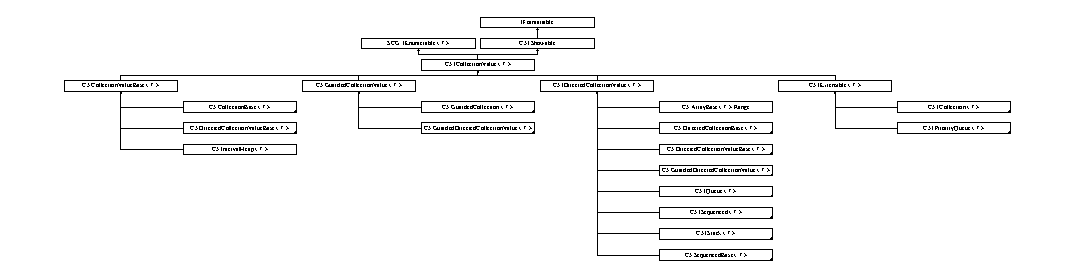
\includegraphics[height=3.268482cm]{interface_c5_1_1_i_collection_value}
\end{center}
\end{figure}
\subsection*{Public Member Functions}
\begin{DoxyCompactItemize}
\item 
void \hyperlink{interface_c5_1_1_i_collection_value_aced299d8dce69c33ff75b598e39581d1}{Copy\+To} (T\mbox{[}$\,$\mbox{]} array, int index)
\begin{DoxyCompactList}\small\item\em Copy the items of this collection to a contiguous part of an array. \end{DoxyCompactList}\item 
T\mbox{[}$\,$\mbox{]} \hyperlink{interface_c5_1_1_i_collection_value_ad76547324e71a04e92076b2e55239bbb}{To\+Array} ()
\begin{DoxyCompactList}\small\item\em Create an array with the items of this collection (in the same order as an enumerator would output them). \end{DoxyCompactList}\item 
void \hyperlink{interface_c5_1_1_i_collection_value_aadcb9ce9d9362c0ade0c7d620e3cc182}{Apply} (Action$<$ T $>$ action)
\begin{DoxyCompactList}\small\item\em Apply a delegate to all items of this collection. \end{DoxyCompactList}\item 
bool \hyperlink{interface_c5_1_1_i_collection_value_a3c20f35782dbd046f9aba5ec13dad789}{Exists} (Func$<$ T, bool $>$ predicate)
\begin{DoxyCompactList}\small\item\em Check if there exists an item that satisfies a specific predicate in this collection. \end{DoxyCompactList}\item 
bool \hyperlink{interface_c5_1_1_i_collection_value_a3e175f833398fa6a6cde45e4948bc152}{Find} (Func$<$ T, bool $>$ predicate, out T item)
\begin{DoxyCompactList}\small\item\em Check if there exists an item that satisfies a specific predicate in this collection and return the first one in enumeration order. \end{DoxyCompactList}\item 
bool \hyperlink{interface_c5_1_1_i_collection_value_a099c3a257e5c0b7212e34e52a4a4bda2}{All} (Func$<$ T, bool $>$ predicate)
\begin{DoxyCompactList}\small\item\em Check if all items in this collection satisfies a specific predicate. \end{DoxyCompactList}\item 
T \hyperlink{interface_c5_1_1_i_collection_value_af72d52ddd8ea4130d508e1cf020cf7eb}{Choose} ()
\begin{DoxyCompactList}\small\item\em Choose some item of this collection. \end{DoxyCompactList}\item 
S\+C\+G.\+I\+Enumerable$<$ T $>$ \hyperlink{interface_c5_1_1_i_collection_value_a485e8b464ed5dfb5f2ff5dc10a8a62d6}{Filter} (Func$<$ T, bool $>$ filter)
\begin{DoxyCompactList}\small\item\em Create an enumerable, enumerating the items of this collection that satisfies a certain condition. \end{DoxyCompactList}\end{DoxyCompactItemize}
\subsection*{Properties}
\begin{DoxyCompactItemize}
\item 
\hyperlink{namespace_c5_a9143bfd561fffa025d21561674758008}{Event\+Type\+Enum} \hyperlink{interface_c5_1_1_i_collection_value_ac19b17d9b2ca7f2717013e4a8076e481}{Listenable\+Events}\hspace{0.3cm}{\ttfamily  \mbox{[}get\mbox{]}}
\begin{DoxyCompactList}\small\item\em A flag bitmap of the events subscribable to by this collection. \end{DoxyCompactList}\item 
\hyperlink{namespace_c5_a9143bfd561fffa025d21561674758008}{Event\+Type\+Enum} \hyperlink{interface_c5_1_1_i_collection_value_a255e04159eaa809e157ce453dc4b2340}{Active\+Events}\hspace{0.3cm}{\ttfamily  \mbox{[}get\mbox{]}}
\begin{DoxyCompactList}\small\item\em A flag bitmap of the events currently subscribed to by this collection. \end{DoxyCompactList}\item 
bool \hyperlink{interface_c5_1_1_i_collection_value_af731142c68c50403553a545318dcae01}{Is\+Empty}\hspace{0.3cm}{\ttfamily  \mbox{[}get\mbox{]}}
\item 
int \hyperlink{interface_c5_1_1_i_collection_value_ac02f774c320d7e93e3020ac124de5c96}{Count}\hspace{0.3cm}{\ttfamily  \mbox{[}get\mbox{]}}
\item 
\hyperlink{namespace_c5_a615ba88dcdaa8d5a3c5f833a73d7fad6}{Speed} \hyperlink{interface_c5_1_1_i_collection_value_aeaf5f215b7f6b1b3aec0a8cd939ea1a9}{Count\+Speed}\hspace{0.3cm}{\ttfamily  \mbox{[}get\mbox{]}}
\begin{DoxyCompactList}\small\item\em The value is symbolic indicating the type of asymptotic complexity in terms of the size of this collection (worst-\/case or amortized as relevant). \end{DoxyCompactList}\end{DoxyCompactItemize}
\subsection*{Events}
\begin{DoxyCompactItemize}
\item 
Collection\+Changed\+Handler$<$ T $>$ \hyperlink{interface_c5_1_1_i_collection_value_a50d218d2c7a194c1a641e14d167b7412}{Collection\+Changed}
\begin{DoxyCompactList}\small\item\em The change event. Will be raised for every change operation on the collection. \end{DoxyCompactList}\item 
Collection\+Cleared\+Handler$<$ T $>$ \hyperlink{interface_c5_1_1_i_collection_value_abfc456208223df571826f444d368f851}{Collection\+Cleared}
\begin{DoxyCompactList}\small\item\em The change event. Will be raised for every clear operation on the collection. \end{DoxyCompactList}\item 
Items\+Added\+Handler$<$ T $>$ \hyperlink{interface_c5_1_1_i_collection_value_a22cf109895d493a5627162f7b5c4041b}{Items\+Added}
\begin{DoxyCompactList}\small\item\em The item added event. Will be raised for every individual addition to the collection. \end{DoxyCompactList}\item 
Item\+Inserted\+Handler$<$ T $>$ \hyperlink{interface_c5_1_1_i_collection_value_a2677a887fe66bbb35811797a04ba9a46}{Item\+Inserted}
\begin{DoxyCompactList}\small\item\em The item inserted event. Will be raised for every individual insertion to the collection. \end{DoxyCompactList}\item 
Items\+Removed\+Handler$<$ T $>$ \hyperlink{interface_c5_1_1_i_collection_value_a5c228bd1f7d517ff48ab6dfc19965c25}{Items\+Removed}
\begin{DoxyCompactList}\small\item\em The item removed event. Will be raised for every individual removal from the collection. \end{DoxyCompactList}\item 
Item\+Removed\+At\+Handler$<$ T $>$ \hyperlink{interface_c5_1_1_i_collection_value_aeb3b4f97b700058c5196d7a8d1241ede}{Item\+Removed\+At}
\begin{DoxyCompactList}\small\item\em The item removed at event. Will be raised for every individual removal at from the collection. \end{DoxyCompactList}\end{DoxyCompactItemize}


\subsection{Detailed Description}
A generic collection that may be enumerated and can answer efficiently how many items it contains. Like 

{\ttfamily I\+Enumerable$<$T$>$}, this interface does not prescribe any operations to initialize or update the collection. The main usage for this interface is to be the return type of query operations on generic collection. 

\subsection{Member Function Documentation}
\hypertarget{interface_c5_1_1_i_collection_value_a099c3a257e5c0b7212e34e52a4a4bda2}{}\index{C5\+::\+I\+Collection\+Value@{C5\+::\+I\+Collection\+Value}!All@{All}}
\index{All@{All}!C5\+::\+I\+Collection\+Value@{C5\+::\+I\+Collection\+Value}}
\subsubsection[{All(\+Func$<$ T, bool $>$ predicate)}]{\setlength{\rightskip}{0pt plus 5cm}bool {\bf C5.\+I\+Collection\+Value}$<$ T $>$.All (
\begin{DoxyParamCaption}
\item[{Func$<$ T, bool $>$}]{predicate}
\end{DoxyParamCaption}
)}\label{interface_c5_1_1_i_collection_value_a099c3a257e5c0b7212e34e52a4a4bda2}


Check if all items in this collection satisfies a specific predicate. 


\begin{DoxyParams}{Parameters}
{\em predicate} & A delegate (T\+:\+Func`2 with 
\begin{DoxyCode}
R == \textcolor{keywordtype}{bool}
\end{DoxyCode}
) defining the predicate\\
\hline
\end{DoxyParams}
\begin{DoxyReturn}{Returns}
True if all items satisfies the predicate
\end{DoxyReturn}


Implemented in \hyperlink{class_c5_1_1_wrapped_array_a2b0d022ae85980d92ad40df11f59cf7e}{C5.\+Wrapped\+Array$<$ T $>$}, \hyperlink{class_c5_1_1_collection_value_base_ad13a5bb7f735bf175add1e275b6d64ab}{C5.\+Collection\+Value\+Base$<$ T $>$}, and \hyperlink{class_c5_1_1_guarded_collection_value_a0fda465306c55a4dde41b5eecdb1180a}{C5.\+Guarded\+Collection\+Value$<$ T $>$}.

\hypertarget{interface_c5_1_1_i_collection_value_aadcb9ce9d9362c0ade0c7d620e3cc182}{}\index{C5\+::\+I\+Collection\+Value@{C5\+::\+I\+Collection\+Value}!Apply@{Apply}}
\index{Apply@{Apply}!C5\+::\+I\+Collection\+Value@{C5\+::\+I\+Collection\+Value}}
\subsubsection[{Apply(\+Action$<$ T $>$ action)}]{\setlength{\rightskip}{0pt plus 5cm}void {\bf C5.\+I\+Collection\+Value}$<$ T $>$.Apply (
\begin{DoxyParamCaption}
\item[{Action$<$ T $>$}]{action}
\end{DoxyParamCaption}
)}\label{interface_c5_1_1_i_collection_value_aadcb9ce9d9362c0ade0c7d620e3cc182}


Apply a delegate to all items of this collection. 


\begin{DoxyParams}{Parameters}
{\em action} & The delegate to apply\\
\hline
\end{DoxyParams}


Implemented in \hyperlink{class_c5_1_1_wrapped_array_a05225daca0b5a607afd5c049ca41da0b}{C5.\+Wrapped\+Array$<$ T $>$}, \hyperlink{class_c5_1_1_collection_value_base_a1de9661198b86224773dcdc9d1678020}{C5.\+Collection\+Value\+Base$<$ T $>$}, and \hyperlink{class_c5_1_1_guarded_collection_value_a212d1ea950a6096f846987476c9e2aa6}{C5.\+Guarded\+Collection\+Value$<$ T $>$}.

\hypertarget{interface_c5_1_1_i_collection_value_af72d52ddd8ea4130d508e1cf020cf7eb}{}\index{C5\+::\+I\+Collection\+Value@{C5\+::\+I\+Collection\+Value}!Choose@{Choose}}
\index{Choose@{Choose}!C5\+::\+I\+Collection\+Value@{C5\+::\+I\+Collection\+Value}}
\subsubsection[{Choose()}]{\setlength{\rightskip}{0pt plus 5cm}T {\bf C5.\+I\+Collection\+Value}$<$ T $>$.Choose (
\begin{DoxyParamCaption}
{}
\end{DoxyParamCaption}
)}\label{interface_c5_1_1_i_collection_value_af72d52ddd8ea4130d508e1cf020cf7eb}


Choose some item of this collection. 

Implementations must assure that the item returned may be efficiently removed.

Implementors may decide to implement this method in a way such that repeated calls do not necessarily give the same result, i.\+e. so that the result of the following test is undetermined\+: {\ttfamily coll.\+Choose() == coll.\+Choose()}


\begin{DoxyExceptions}{Exceptions}
{\em \hyperlink{class_c5_1_1_no_such_item_exception}{No\+Such\+Item\+Exception}} & if collection is empty.\\
\hline
\end{DoxyExceptions}
\begin{DoxyReturn}{Returns}

\end{DoxyReturn}


Implemented in \hyperlink{class_c5_1_1_hashed_linked_list_a8f4365d623d3424943b1891e998fc90d}{C5.\+Hashed\+Linked\+List$<$ T $>$}, \hyperlink{class_c5_1_1_linked_list_a50a8bc512629f661b2e98a1dc860cc9f}{C5.\+Linked\+List$<$ T $>$}, \hyperlink{class_c5_1_1_array_base_1_1_range_a914b2f3399f5286d462af7f1837373db}{C5.\+Array\+Base$<$ T $>$.\+Range}, \hyperlink{class_c5_1_1_array_base_a1d5f2551ce0fb795a5f2105fcb958de8}{C5.\+Array\+Base$<$ T $>$}, \hyperlink{class_c5_1_1_wrapped_array_ad42ddaec045d78e9d559b12279f7598a}{C5.\+Wrapped\+Array$<$ T $>$}, \hyperlink{class_c5_1_1_hash_set_a6bac17b51f5b2a569a0df8e0c46fe78f}{C5.\+Hash\+Set$<$ T $>$}, \hyperlink{class_c5_1_1_hash_bag_ac17786a0542bbe968fc662d5e2749265}{C5.\+Hash\+Bag$<$ T $>$}, \hyperlink{class_c5_1_1_tree_bag_a7b05001428a9e4605f556683a9bea20a}{C5.\+Tree\+Bag$<$ T $>$}, \hyperlink{class_c5_1_1_tree_set_aa4dd484b7c4363226e1053c8b2edd851}{C5.\+Tree\+Set$<$ T $>$}, \hyperlink{class_c5_1_1_collection_value_base_ad7b8bd01dfd7ea8480a972f02a81608b}{C5.\+Collection\+Value\+Base$<$ T $>$}, \hyperlink{class_c5_1_1_interval_heap_a0d5fe1b0687d6ef002a17c6e46900772}{C5.\+Interval\+Heap$<$ T $>$}, \hyperlink{class_c5_1_1_guarded_collection_value_ac1c427d873e650f819d6c662515dadd1}{C5.\+Guarded\+Collection\+Value$<$ T $>$}, and \hyperlink{class_c5_1_1_circular_queue_aeabd2341783df834015d58b04c0c0a11}{C5.\+Circular\+Queue$<$ T $>$}.

\hypertarget{interface_c5_1_1_i_collection_value_aced299d8dce69c33ff75b598e39581d1}{}\index{C5\+::\+I\+Collection\+Value@{C5\+::\+I\+Collection\+Value}!Copy\+To@{Copy\+To}}
\index{Copy\+To@{Copy\+To}!C5\+::\+I\+Collection\+Value@{C5\+::\+I\+Collection\+Value}}
\subsubsection[{Copy\+To(\+T[] array, int index)}]{\setlength{\rightskip}{0pt plus 5cm}void {\bf C5.\+I\+Collection\+Value}$<$ T $>$.Copy\+To (
\begin{DoxyParamCaption}
\item[{T\mbox{[}$\,$\mbox{]}}]{array, }
\item[{int}]{index}
\end{DoxyParamCaption}
)}\label{interface_c5_1_1_i_collection_value_aced299d8dce69c33ff75b598e39581d1}


Copy the items of this collection to a contiguous part of an array. 


\begin{DoxyParams}{Parameters}
{\em array} & The array to copy to\\
\hline
{\em index} & The index at which to copy the first item\\
\hline
\end{DoxyParams}


Implemented in \hyperlink{interface_c5_1_1_i_list_a6fef986271bdc88a6f38cb15bd15690f}{C5.\+I\+List$<$ T $>$}, \hyperlink{class_c5_1_1_wrapped_array_a3dfd50eb13f5b3f90445e217214fae96}{C5.\+Wrapped\+Array$<$ T $>$}, \hyperlink{class_c5_1_1_hash_bag_ad7ffdb5c882c290aa8b398d499a9d2ac}{C5.\+Hash\+Bag$<$ T $>$}, \hyperlink{class_c5_1_1_collection_value_base_ab238770f168304e89664f814925522da}{C5.\+Collection\+Value\+Base$<$ T $>$}, \hyperlink{interface_c5_1_1_i_collection_aa2f928b7057eb84a1572307123e8239e}{C5.\+I\+Collection$<$ T $>$}, and \hyperlink{class_c5_1_1_guarded_collection_value_ae8d04b8fd3c59fe20bdc4a99fb1134f2}{C5.\+Guarded\+Collection\+Value$<$ T $>$}.

\hypertarget{interface_c5_1_1_i_collection_value_a3c20f35782dbd046f9aba5ec13dad789}{}\index{C5\+::\+I\+Collection\+Value@{C5\+::\+I\+Collection\+Value}!Exists@{Exists}}
\index{Exists@{Exists}!C5\+::\+I\+Collection\+Value@{C5\+::\+I\+Collection\+Value}}
\subsubsection[{Exists(\+Func$<$ T, bool $>$ predicate)}]{\setlength{\rightskip}{0pt plus 5cm}bool {\bf C5.\+I\+Collection\+Value}$<$ T $>$.Exists (
\begin{DoxyParamCaption}
\item[{Func$<$ T, bool $>$}]{predicate}
\end{DoxyParamCaption}
)}\label{interface_c5_1_1_i_collection_value_a3c20f35782dbd046f9aba5ec13dad789}


Check if there exists an item that satisfies a specific predicate in this collection. 


\begin{DoxyParams}{Parameters}
{\em predicate} & A delegate (T\+:\+Func`2 with 
\begin{DoxyCode}
R == \textcolor{keywordtype}{bool}
\end{DoxyCode}
) defining the predicate\\
\hline
\end{DoxyParams}
\begin{DoxyReturn}{Returns}
True is such an item exists
\end{DoxyReturn}


Implemented in \hyperlink{class_c5_1_1_wrapped_array_a46a3457811b2f237cbf7ed19d11baa0e}{C5.\+Wrapped\+Array$<$ T $>$}, \hyperlink{class_c5_1_1_collection_value_base_af8e9e1630489ab12d89363cf4ab0e2ab}{C5.\+Collection\+Value\+Base$<$ T $>$}, and \hyperlink{class_c5_1_1_guarded_collection_value_a0c3c6dfb00cd3206e56939a8a49ff622}{C5.\+Guarded\+Collection\+Value$<$ T $>$}.

\hypertarget{interface_c5_1_1_i_collection_value_a485e8b464ed5dfb5f2ff5dc10a8a62d6}{}\index{C5\+::\+I\+Collection\+Value@{C5\+::\+I\+Collection\+Value}!Filter@{Filter}}
\index{Filter@{Filter}!C5\+::\+I\+Collection\+Value@{C5\+::\+I\+Collection\+Value}}
\subsubsection[{Filter(\+Func$<$ T, bool $>$ filter)}]{\setlength{\rightskip}{0pt plus 5cm}S\+C\+G.\+I\+Enumerable$<$T$>$ {\bf C5.\+I\+Collection\+Value}$<$ T $>$.Filter (
\begin{DoxyParamCaption}
\item[{Func$<$ T, bool $>$}]{filter}
\end{DoxyParamCaption}
)}\label{interface_c5_1_1_i_collection_value_a485e8b464ed5dfb5f2ff5dc10a8a62d6}


Create an enumerable, enumerating the items of this collection that satisfies a certain condition. 


\begin{DoxyParams}{Parameters}
{\em filter} & The T-\/$>$bool filter delegate defining the condition\\
\hline
\end{DoxyParams}
\begin{DoxyReturn}{Returns}
The filtered enumerable
\end{DoxyReturn}


Implemented in \hyperlink{class_c5_1_1_hashed_linked_list_ad092b0255821d358df6cfe045870e256}{C5.\+Hashed\+Linked\+List$<$ T $>$}, \hyperlink{class_c5_1_1_linked_list_a5027335e5234dc6a6e3a164d79ccae62}{C5.\+Linked\+List$<$ T $>$}, \hyperlink{class_c5_1_1_wrapped_array_a3eee2c5f8d76cd8c3f0d26fa0488fcb7}{C5.\+Wrapped\+Array$<$ T $>$}, \hyperlink{class_c5_1_1_collection_value_base_a1e67c05020e8bebf39e0ddc9f55e5f32}{C5.\+Collection\+Value\+Base$<$ T $>$}, and \hyperlink{class_c5_1_1_guarded_collection_value_a69ab914af51ee2fefc9a0e874e544b3f}{C5.\+Guarded\+Collection\+Value$<$ T $>$}.

\hypertarget{interface_c5_1_1_i_collection_value_a3e175f833398fa6a6cde45e4948bc152}{}\index{C5\+::\+I\+Collection\+Value@{C5\+::\+I\+Collection\+Value}!Find@{Find}}
\index{Find@{Find}!C5\+::\+I\+Collection\+Value@{C5\+::\+I\+Collection\+Value}}
\subsubsection[{Find(\+Func$<$ T, bool $>$ predicate, out T item)}]{\setlength{\rightskip}{0pt plus 5cm}bool {\bf C5.\+I\+Collection\+Value}$<$ T $>$.Find (
\begin{DoxyParamCaption}
\item[{Func$<$ T, bool $>$}]{predicate, }
\item[{out T}]{item}
\end{DoxyParamCaption}
)}\label{interface_c5_1_1_i_collection_value_a3e175f833398fa6a6cde45e4948bc152}


Check if there exists an item that satisfies a specific predicate in this collection and return the first one in enumeration order. 


\begin{DoxyParams}{Parameters}
{\em predicate} & A delegate (T\+:\+Func`2 with 
\begin{DoxyCode}
R == \textcolor{keywordtype}{bool}
\end{DoxyCode}
) defining the predicate\\
\hline
{\em item} & \\
\hline
\end{DoxyParams}
\begin{DoxyReturn}{Returns}
True is such an item exists
\end{DoxyReturn}


Implemented in \hyperlink{class_c5_1_1_wrapped_array_acc9f79f847e3906ccf84a2543090bcb0}{C5.\+Wrapped\+Array$<$ T $>$}, \hyperlink{class_c5_1_1_collection_value_base_a90b979207d15086a9b64c9c689e17d4f}{C5.\+Collection\+Value\+Base$<$ T $>$}, and \hyperlink{class_c5_1_1_guarded_collection_value_a7bccfb81326892afd0ae30ac5e55cdaa}{C5.\+Guarded\+Collection\+Value$<$ T $>$}.

\hypertarget{interface_c5_1_1_i_collection_value_ad76547324e71a04e92076b2e55239bbb}{}\index{C5\+::\+I\+Collection\+Value@{C5\+::\+I\+Collection\+Value}!To\+Array@{To\+Array}}
\index{To\+Array@{To\+Array}!C5\+::\+I\+Collection\+Value@{C5\+::\+I\+Collection\+Value}}
\subsubsection[{To\+Array()}]{\setlength{\rightskip}{0pt plus 5cm}T \mbox{[}$\,$\mbox{]} {\bf C5.\+I\+Collection\+Value}$<$ T $>$.To\+Array (
\begin{DoxyParamCaption}
{}
\end{DoxyParamCaption}
)}\label{interface_c5_1_1_i_collection_value_ad76547324e71a04e92076b2e55239bbb}


Create an array with the items of this collection (in the same order as an enumerator would output them). 

\begin{DoxyReturn}{Returns}
The array
\end{DoxyReturn}


Implemented in \hyperlink{class_c5_1_1_array_base_a16ffcc583a32065194b3ea27d4a43cd4}{C5.\+Array\+Base$<$ T $>$}, \hyperlink{class_c5_1_1_wrapped_array_a58fc7250416e58474a98d17a538fb9e2}{C5.\+Wrapped\+Array$<$ T $>$}, \hyperlink{class_c5_1_1_hash_set_ad6e22ebc64d9f8c96b805547d5873023}{C5.\+Hash\+Set$<$ T $>$}, \hyperlink{class_c5_1_1_collection_value_base_a740757aebaa1365811e76729e59f338d}{C5.\+Collection\+Value\+Base$<$ T $>$}, \hyperlink{class_c5_1_1_hash_bag_a7be4bcb7a5ef7f9414a33cfb9439e15e}{C5.\+Hash\+Bag$<$ T $>$}, and \hyperlink{class_c5_1_1_guarded_collection_value_ab492c6c9d057b13d2ccbb7ebc259a4f6}{C5.\+Guarded\+Collection\+Value$<$ T $>$}.



\subsection{Property Documentation}
\hypertarget{interface_c5_1_1_i_collection_value_a255e04159eaa809e157ce453dc4b2340}{}\index{C5\+::\+I\+Collection\+Value@{C5\+::\+I\+Collection\+Value}!Active\+Events@{Active\+Events}}
\index{Active\+Events@{Active\+Events}!C5\+::\+I\+Collection\+Value@{C5\+::\+I\+Collection\+Value}}
\subsubsection[{Active\+Events}]{\setlength{\rightskip}{0pt plus 5cm}{\bf Event\+Type\+Enum} {\bf C5.\+I\+Collection\+Value}$<$ T $>$.Active\+Events\hspace{0.3cm}{\ttfamily [get]}}\label{interface_c5_1_1_i_collection_value_a255e04159eaa809e157ce453dc4b2340}


A flag bitmap of the events currently subscribed to by this collection. 

\hypertarget{interface_c5_1_1_i_collection_value_ac02f774c320d7e93e3020ac124de5c96}{}\index{C5\+::\+I\+Collection\+Value@{C5\+::\+I\+Collection\+Value}!Count@{Count}}
\index{Count@{Count}!C5\+::\+I\+Collection\+Value@{C5\+::\+I\+Collection\+Value}}
\subsubsection[{Count}]{\setlength{\rightskip}{0pt plus 5cm}int {\bf C5.\+I\+Collection\+Value}$<$ T $>$.Count\hspace{0.3cm}{\ttfamily [get]}}\label{interface_c5_1_1_i_collection_value_ac02f774c320d7e93e3020ac124de5c96}




The number of items in this collection\hypertarget{interface_c5_1_1_i_collection_value_aeaf5f215b7f6b1b3aec0a8cd939ea1a9}{}\index{C5\+::\+I\+Collection\+Value@{C5\+::\+I\+Collection\+Value}!Count\+Speed@{Count\+Speed}}
\index{Count\+Speed@{Count\+Speed}!C5\+::\+I\+Collection\+Value@{C5\+::\+I\+Collection\+Value}}
\subsubsection[{Count\+Speed}]{\setlength{\rightskip}{0pt plus 5cm}{\bf Speed} {\bf C5.\+I\+Collection\+Value}$<$ T $>$.Count\+Speed\hspace{0.3cm}{\ttfamily [get]}}\label{interface_c5_1_1_i_collection_value_aeaf5f215b7f6b1b3aec0a8cd939ea1a9}


The value is symbolic indicating the type of asymptotic complexity in terms of the size of this collection (worst-\/case or amortized as relevant). 

A characterization of the speed of the {\ttfamily Count} property in this collection.\hypertarget{interface_c5_1_1_i_collection_value_af731142c68c50403553a545318dcae01}{}\index{C5\+::\+I\+Collection\+Value@{C5\+::\+I\+Collection\+Value}!Is\+Empty@{Is\+Empty}}
\index{Is\+Empty@{Is\+Empty}!C5\+::\+I\+Collection\+Value@{C5\+::\+I\+Collection\+Value}}
\subsubsection[{Is\+Empty}]{\setlength{\rightskip}{0pt plus 5cm}bool {\bf C5.\+I\+Collection\+Value}$<$ T $>$.Is\+Empty\hspace{0.3cm}{\ttfamily [get]}}\label{interface_c5_1_1_i_collection_value_af731142c68c50403553a545318dcae01}




True if this collection is empty.\hypertarget{interface_c5_1_1_i_collection_value_ac19b17d9b2ca7f2717013e4a8076e481}{}\index{C5\+::\+I\+Collection\+Value@{C5\+::\+I\+Collection\+Value}!Listenable\+Events@{Listenable\+Events}}
\index{Listenable\+Events@{Listenable\+Events}!C5\+::\+I\+Collection\+Value@{C5\+::\+I\+Collection\+Value}}
\subsubsection[{Listenable\+Events}]{\setlength{\rightskip}{0pt plus 5cm}{\bf Event\+Type\+Enum} {\bf C5.\+I\+Collection\+Value}$<$ T $>$.Listenable\+Events\hspace{0.3cm}{\ttfamily [get]}}\label{interface_c5_1_1_i_collection_value_ac19b17d9b2ca7f2717013e4a8076e481}


A flag bitmap of the events subscribable to by this collection. 



\subsection{Event Documentation}
\hypertarget{interface_c5_1_1_i_collection_value_a50d218d2c7a194c1a641e14d167b7412}{}\index{C5\+::\+I\+Collection\+Value@{C5\+::\+I\+Collection\+Value}!Collection\+Changed@{Collection\+Changed}}
\index{Collection\+Changed@{Collection\+Changed}!C5\+::\+I\+Collection\+Value@{C5\+::\+I\+Collection\+Value}}
\subsubsection[{Collection\+Changed}]{\setlength{\rightskip}{0pt plus 5cm}Collection\+Changed\+Handler$<$T$>$ {\bf C5.\+I\+Collection\+Value}$<$ T $>$.Collection\+Changed}\label{interface_c5_1_1_i_collection_value_a50d218d2c7a194c1a641e14d167b7412}


The change event. Will be raised for every change operation on the collection. 

\hypertarget{interface_c5_1_1_i_collection_value_abfc456208223df571826f444d368f851}{}\index{C5\+::\+I\+Collection\+Value@{C5\+::\+I\+Collection\+Value}!Collection\+Cleared@{Collection\+Cleared}}
\index{Collection\+Cleared@{Collection\+Cleared}!C5\+::\+I\+Collection\+Value@{C5\+::\+I\+Collection\+Value}}
\subsubsection[{Collection\+Cleared}]{\setlength{\rightskip}{0pt plus 5cm}Collection\+Cleared\+Handler$<$T$>$ {\bf C5.\+I\+Collection\+Value}$<$ T $>$.Collection\+Cleared}\label{interface_c5_1_1_i_collection_value_abfc456208223df571826f444d368f851}


The change event. Will be raised for every clear operation on the collection. 

\hypertarget{interface_c5_1_1_i_collection_value_a2677a887fe66bbb35811797a04ba9a46}{}\index{C5\+::\+I\+Collection\+Value@{C5\+::\+I\+Collection\+Value}!Item\+Inserted@{Item\+Inserted}}
\index{Item\+Inserted@{Item\+Inserted}!C5\+::\+I\+Collection\+Value@{C5\+::\+I\+Collection\+Value}}
\subsubsection[{Item\+Inserted}]{\setlength{\rightskip}{0pt plus 5cm}Item\+Inserted\+Handler$<$T$>$ {\bf C5.\+I\+Collection\+Value}$<$ T $>$.Item\+Inserted}\label{interface_c5_1_1_i_collection_value_a2677a887fe66bbb35811797a04ba9a46}


The item inserted event. Will be raised for every individual insertion to the collection. 

\hypertarget{interface_c5_1_1_i_collection_value_aeb3b4f97b700058c5196d7a8d1241ede}{}\index{C5\+::\+I\+Collection\+Value@{C5\+::\+I\+Collection\+Value}!Item\+Removed\+At@{Item\+Removed\+At}}
\index{Item\+Removed\+At@{Item\+Removed\+At}!C5\+::\+I\+Collection\+Value@{C5\+::\+I\+Collection\+Value}}
\subsubsection[{Item\+Removed\+At}]{\setlength{\rightskip}{0pt plus 5cm}Item\+Removed\+At\+Handler$<$T$>$ {\bf C5.\+I\+Collection\+Value}$<$ T $>$.Item\+Removed\+At}\label{interface_c5_1_1_i_collection_value_aeb3b4f97b700058c5196d7a8d1241ede}


The item removed at event. Will be raised for every individual removal at from the collection. 

\hypertarget{interface_c5_1_1_i_collection_value_a22cf109895d493a5627162f7b5c4041b}{}\index{C5\+::\+I\+Collection\+Value@{C5\+::\+I\+Collection\+Value}!Items\+Added@{Items\+Added}}
\index{Items\+Added@{Items\+Added}!C5\+::\+I\+Collection\+Value@{C5\+::\+I\+Collection\+Value}}
\subsubsection[{Items\+Added}]{\setlength{\rightskip}{0pt plus 5cm}Items\+Added\+Handler$<$T$>$ {\bf C5.\+I\+Collection\+Value}$<$ T $>$.Items\+Added}\label{interface_c5_1_1_i_collection_value_a22cf109895d493a5627162f7b5c4041b}


The item added event. Will be raised for every individual addition to the collection. 

\hypertarget{interface_c5_1_1_i_collection_value_a5c228bd1f7d517ff48ab6dfc19965c25}{}\index{C5\+::\+I\+Collection\+Value@{C5\+::\+I\+Collection\+Value}!Items\+Removed@{Items\+Removed}}
\index{Items\+Removed@{Items\+Removed}!C5\+::\+I\+Collection\+Value@{C5\+::\+I\+Collection\+Value}}
\subsubsection[{Items\+Removed}]{\setlength{\rightskip}{0pt plus 5cm}Items\+Removed\+Handler$<$T$>$ {\bf C5.\+I\+Collection\+Value}$<$ T $>$.Items\+Removed}\label{interface_c5_1_1_i_collection_value_a5c228bd1f7d517ff48ab6dfc19965c25}


The item removed event. Will be raised for every individual removal from the collection. 



The documentation for this interface was generated from the following file\+:\begin{DoxyCompactItemize}
\item 
C\+:/\+Users/rasmusl/\+Source/\+Repos/\+C5/\+C5/\hyperlink{_interfaces_8cs}{Interfaces.\+cs}\end{DoxyCompactItemize}

\hypertarget{interface_c5_1_1_i_dictionary}{}\section{C5.\+I\+Dictionary$<$ K, V $>$ Interface Template Reference}
\label{interface_c5_1_1_i_dictionary}\index{C5.\+I\+Dictionary$<$ K, V $>$@{C5.\+I\+Dictionary$<$ K, V $>$}}


A dictionary with keys of type K and values of type V. Equivalent to a finite partial map from K to V.  


Inheritance diagram for C5.\+I\+Dictionary$<$ K, V $>$\+:\begin{figure}[H]
\begin{center}
\leavevmode
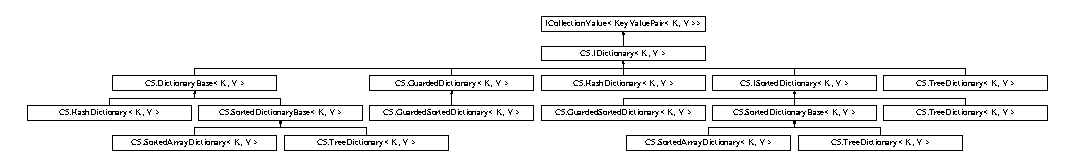
\includegraphics[height=1.801802cm]{interface_c5_1_1_i_dictionary}
\end{center}
\end{figure}
\subsection*{Public Member Functions}
\begin{DoxyCompactItemize}
\item 
void \hyperlink{interface_c5_1_1_i_dictionary_a7e3eefcf603863fe54ce86080bbc07d7}{Add} (K key, V val)
\begin{DoxyCompactList}\small\item\em Add a new (key, value) pair (a mapping) to the dictionary. \end{DoxyCompactList}\item 
void \hyperlink{interface_c5_1_1_i_dictionary_aa6cfac9dc29e58092c4dd65190f431af}{Add\+All$<$ U, W $>$} (S\+C\+G.\+I\+Enumerable$<$ \hyperlink{struct_c5_1_1_key_value_pair}{Key\+Value\+Pair}$<$ U, W $>$$>$ entries)
\begin{DoxyCompactList}\small\item\em Add the entries from a collection of T\+:\+C5.\+Key\+Value\+Pair`2 pairs to this dictionary. \end{DoxyCompactList}\item 
bool \hyperlink{interface_c5_1_1_i_dictionary_a18a33ccf0bac3ac7ef8046850104c5d5}{Contains\+All$<$ H $>$} (S\+C\+G.\+I\+Enumerable$<$ H $>$ items)
\begin{DoxyCompactList}\small\item\em Check whether this collection contains all the values in another collection. If this collection has bag semantics ( \end{DoxyCompactList}\item 
bool \hyperlink{interface_c5_1_1_i_dictionary_a35b1f0b9f0e0c555246b9154b6e45ab5}{Remove} (K key)
\begin{DoxyCompactList}\small\item\em Remove an entry with a given key from the dictionary \end{DoxyCompactList}\item 
bool \hyperlink{interface_c5_1_1_i_dictionary_a24f34aa709dc1157536afb1d251135d5}{Remove} (K key, out V val)
\begin{DoxyCompactList}\small\item\em Remove an entry with a given key from the dictionary and report its value. \end{DoxyCompactList}\item 
void \hyperlink{interface_c5_1_1_i_dictionary_a9eb0026921a6b39c781495efd65dc82b}{Clear} ()
\begin{DoxyCompactList}\small\item\em Remove all entries from the dictionary \end{DoxyCompactList}\item 
bool \hyperlink{interface_c5_1_1_i_dictionary_a08f4af4a7f427e8e9022a13f2e79c031}{Contains} (K key)
\begin{DoxyCompactList}\small\item\em Check if there is an entry with a specified key \end{DoxyCompactList}\item 
bool \hyperlink{interface_c5_1_1_i_dictionary_a40f6257961c1578fea31f0507cd5c28e}{Find} (ref K key, out V val)
\begin{DoxyCompactList}\small\item\em Check if there is an entry with a specified key and report the corresponding value if found. This can be seen as a safe form of \char`\"{}val = this\mbox{[}key\mbox{]}\char`\"{}. \end{DoxyCompactList}\item 
bool \hyperlink{interface_c5_1_1_i_dictionary_aa1af112490cca3ed7816d47b9127dace}{Update} (K key, V val)
\begin{DoxyCompactList}\small\item\em Look for a specific key in the dictionary and if found replace the value with a new one. This can be seen as a non-\/adding version of \char`\"{}this\mbox{[}key\mbox{]} = val\char`\"{}. \end{DoxyCompactList}\item 
bool \hyperlink{interface_c5_1_1_i_dictionary_a0338a7b5bfa797aeb75d153faf00dc31}{Update} (K key, V val, out V oldval)
\begin{DoxyCompactList}\small\item\em Look for a specific key in the dictionary and if found replace the value with a new one. This can be seen as a non-\/adding version of \char`\"{}this\mbox{[}key\mbox{]} = val\char`\"{} reporting the old value. \end{DoxyCompactList}\item 
bool \hyperlink{interface_c5_1_1_i_dictionary_a1f9f0bd335980be8c24d74470bd19ffc}{Find\+Or\+Add} (K key, ref V val)
\begin{DoxyCompactList}\small\item\em Look for a specific key in the dictionary. If found, report the corresponding value, else add an entry with the key and the supplied value. \end{DoxyCompactList}\item 
bool \hyperlink{interface_c5_1_1_i_dictionary_a9cb26d974f4da6030fe50b4bcc3dc4f1}{Update\+Or\+Add} (K key, V val)
\begin{DoxyCompactList}\small\item\em Update value in dictionary corresponding to key if found, else add new entry. More general than \char`\"{}this\mbox{[}key\mbox{]} = val;\char`\"{} by reporting if key was found. \end{DoxyCompactList}\item 
bool \hyperlink{interface_c5_1_1_i_dictionary_abc8d5a032bbf487db18fc26e31ad512d}{Update\+Or\+Add} (K key, V val, out V oldval)
\begin{DoxyCompactList}\small\item\em Update value in dictionary corresponding to key if found, else add new entry. More general than \char`\"{}this\mbox{[}key\mbox{]} = val;\char`\"{} by reporting if key was found. \end{DoxyCompactList}\item 
bool \hyperlink{interface_c5_1_1_i_dictionary_a659969044740981cdcfe5ee86585104c}{Check} ()
\begin{DoxyCompactList}\small\item\em Check the integrity of the internal data structures of this dictionary. Only avaliable in D\+E\+B\+U\+G builds??? \end{DoxyCompactList}\end{DoxyCompactItemize}
\subsection*{Properties}
\begin{DoxyCompactItemize}
\item 
S\+C\+G.\+I\+Equality\+Comparer$<$ K $>$ \hyperlink{interface_c5_1_1_i_dictionary_a0bf7369acbd3334ece5ce696517678d3}{Equality\+Comparer}\hspace{0.3cm}{\ttfamily  \mbox{[}get\mbox{]}}
\begin{DoxyCompactList}\small\item\em The key equality\+Comparer. \end{DoxyCompactList}\item 
V \hyperlink{interface_c5_1_1_i_dictionary_af9e15cebc5c8d59357b5b3bd9d2a7abd}{this\mbox{[}\+K key\mbox{]}}\hspace{0.3cm}{\ttfamily  \mbox{[}get, set\mbox{]}}
\begin{DoxyCompactList}\small\item\em Indexer for dictionary. \end{DoxyCompactList}\item 
bool \hyperlink{interface_c5_1_1_i_dictionary_ace8a1dded19cb8d2a60c4c7274ebb321}{Is\+Read\+Only}\hspace{0.3cm}{\ttfamily  \mbox{[}get\mbox{]}}
\item 
\hyperlink{interface_c5_1_1_i_collection_value}{I\+Collection\+Value}$<$ K $>$ \hyperlink{interface_c5_1_1_i_dictionary_adc8e64e7f441dbf36723fde4734c19d1}{Keys}\hspace{0.3cm}{\ttfamily  \mbox{[}get\mbox{]}}
\item 
\hyperlink{interface_c5_1_1_i_collection_value}{I\+Collection\+Value}$<$ V $>$ \hyperlink{interface_c5_1_1_i_dictionary_a3c84724a5e4993d0b1e92878829af887}{Values}\hspace{0.3cm}{\ttfamily  \mbox{[}get\mbox{]}}
\item 
Func$<$ K, V $>$ \hyperlink{interface_c5_1_1_i_dictionary_a253959f9511770e1afe1082d871a4489}{Func}\hspace{0.3cm}{\ttfamily  \mbox{[}get\mbox{]}}
\item 
\hyperlink{namespace_c5_a615ba88dcdaa8d5a3c5f833a73d7fad6}{Speed} \hyperlink{interface_c5_1_1_i_dictionary_a25c7daa67a85d9b95b9adc15ec06b8be}{Contains\+Speed}\hspace{0.3cm}{\ttfamily  \mbox{[}get\mbox{]}}
\begin{DoxyCompactList}\small\item\em The value is symbolic indicating the type of asymptotic complexity in terms of the size of this collection (worst-\/case or amortized as relevant). \end{DoxyCompactList}\end{DoxyCompactItemize}


\subsection{Detailed Description}
A dictionary with keys of type K and values of type V. Equivalent to a finite partial map from K to V. 



\subsection{Member Function Documentation}
\hypertarget{interface_c5_1_1_i_dictionary_a7e3eefcf603863fe54ce86080bbc07d7}{}\index{C5\+::\+I\+Dictionary@{C5\+::\+I\+Dictionary}!Add@{Add}}
\index{Add@{Add}!C5\+::\+I\+Dictionary@{C5\+::\+I\+Dictionary}}
\subsubsection[{Add(\+K key, V val)}]{\setlength{\rightskip}{0pt plus 5cm}void {\bf C5.\+I\+Dictionary}$<$ K, V $>$.Add (
\begin{DoxyParamCaption}
\item[{K}]{key, }
\item[{V}]{val}
\end{DoxyParamCaption}
)}\label{interface_c5_1_1_i_dictionary_a7e3eefcf603863fe54ce86080bbc07d7}


Add a new (key, value) pair (a mapping) to the dictionary. 


\begin{DoxyExceptions}{Exceptions}
{\em \hyperlink{class_c5_1_1_duplicate_not_allowed_exception}{Duplicate\+Not\+Allowed\+Exception}} & if there already is an entry with the same key. \\
\hline
\end{DoxyExceptions}
$>$ 
\begin{DoxyParams}{Parameters}
{\em key} & Key to add\\
\hline
{\em val} & Value to add\\
\hline
\end{DoxyParams}


Implemented in \hyperlink{class_c5_1_1_guarded_dictionary_a353f8b07283f31fb34456317bdb9cf43}{C5.\+Guarded\+Dictionary$<$ K, V $>$}, and \hyperlink{class_c5_1_1_dictionary_base_a0d7b0e8b7b2eb71b9478afac991c28b7}{C5.\+Dictionary\+Base$<$ K, V $>$}.

\hypertarget{interface_c5_1_1_i_dictionary_aa6cfac9dc29e58092c4dd65190f431af}{}\index{C5\+::\+I\+Dictionary@{C5\+::\+I\+Dictionary}!Add\+All$<$ U, W $>$@{Add\+All$<$ U, W $>$}}
\index{Add\+All$<$ U, W $>$@{Add\+All$<$ U, W $>$}!C5\+::\+I\+Dictionary@{C5\+::\+I\+Dictionary}}
\subsubsection[{Add\+All$<$ U, W $>$(\+S\+C\+G.\+I\+Enumerable$<$ Key\+Value\+Pair$<$ U, W $>$$>$ entries)}]{\setlength{\rightskip}{0pt plus 5cm}void {\bf C5.\+I\+Dictionary}$<$ K, V $>$.Add\+All$<$ U, W $>$ (
\begin{DoxyParamCaption}
\item[{S\+C\+G.\+I\+Enumerable$<$ {\bf Key\+Value\+Pair}$<$ U, W $>$$>$}]{entries}
\end{DoxyParamCaption}
)}\label{interface_c5_1_1_i_dictionary_aa6cfac9dc29e58092c4dd65190f431af}


Add the entries from a collection of T\+:\+C5.\+Key\+Value\+Pair`2 pairs to this dictionary. 


\begin{DoxyExceptions}{Exceptions}
{\em \hyperlink{class_c5_1_1_duplicate_not_allowed_exception}{Duplicate\+Not\+Allowed\+Exception}} & If the input contains duplicate keys or a key already present in this dictionary.\\
\hline
\end{DoxyExceptions}

\begin{DoxyParams}{Parameters}
{\em entries} & \\
\hline
\end{DoxyParams}
\begin{Desc}
\item[Type Constraints]\begin{description}
\item[{\em U} : {\em K}]\item[{\em W} : {\em V}]\end{description}
\end{Desc}
\hypertarget{interface_c5_1_1_i_dictionary_a659969044740981cdcfe5ee86585104c}{}\index{C5\+::\+I\+Dictionary@{C5\+::\+I\+Dictionary}!Check@{Check}}
\index{Check@{Check}!C5\+::\+I\+Dictionary@{C5\+::\+I\+Dictionary}}
\subsubsection[{Check()}]{\setlength{\rightskip}{0pt plus 5cm}bool {\bf C5.\+I\+Dictionary}$<$ K, V $>$.Check (
\begin{DoxyParamCaption}
{}
\end{DoxyParamCaption}
)}\label{interface_c5_1_1_i_dictionary_a659969044740981cdcfe5ee86585104c}


Check the integrity of the internal data structures of this dictionary. Only avaliable in D\+E\+B\+U\+G builds??? 

\begin{DoxyReturn}{Returns}
True if check does not fail.
\end{DoxyReturn}


Implemented in \hyperlink{class_c5_1_1_guarded_dictionary_a366d84d2fd3b966b091e030cd8ff131b}{C5.\+Guarded\+Dictionary$<$ K, V $>$}, and \hyperlink{class_c5_1_1_dictionary_base_ab72061b2a1b9923c7bc7943d6276892b}{C5.\+Dictionary\+Base$<$ K, V $>$}.

\hypertarget{interface_c5_1_1_i_dictionary_a9eb0026921a6b39c781495efd65dc82b}{}\index{C5\+::\+I\+Dictionary@{C5\+::\+I\+Dictionary}!Clear@{Clear}}
\index{Clear@{Clear}!C5\+::\+I\+Dictionary@{C5\+::\+I\+Dictionary}}
\subsubsection[{Clear()}]{\setlength{\rightskip}{0pt plus 5cm}void {\bf C5.\+I\+Dictionary}$<$ K, V $>$.Clear (
\begin{DoxyParamCaption}
{}
\end{DoxyParamCaption}
)}\label{interface_c5_1_1_i_dictionary_a9eb0026921a6b39c781495efd65dc82b}


Remove all entries from the dictionary 



Implemented in \hyperlink{class_c5_1_1_guarded_dictionary_ac5f23f523e9eae132f4e465eb004be0a}{C5.\+Guarded\+Dictionary$<$ K, V $>$}, and \hyperlink{class_c5_1_1_dictionary_base_ac3a1aa92d354489522afc03f8f303087}{C5.\+Dictionary\+Base$<$ K, V $>$}.

\hypertarget{interface_c5_1_1_i_dictionary_a08f4af4a7f427e8e9022a13f2e79c031}{}\index{C5\+::\+I\+Dictionary@{C5\+::\+I\+Dictionary}!Contains@{Contains}}
\index{Contains@{Contains}!C5\+::\+I\+Dictionary@{C5\+::\+I\+Dictionary}}
\subsubsection[{Contains(\+K key)}]{\setlength{\rightskip}{0pt plus 5cm}bool {\bf C5.\+I\+Dictionary}$<$ K, V $>$.Contains (
\begin{DoxyParamCaption}
\item[{K}]{key}
\end{DoxyParamCaption}
)}\label{interface_c5_1_1_i_dictionary_a08f4af4a7f427e8e9022a13f2e79c031}


Check if there is an entry with a specified key 


\begin{DoxyParams}{Parameters}
{\em key} & The key to look for\\
\hline
\end{DoxyParams}
\begin{DoxyReturn}{Returns}
True if key was found
\end{DoxyReturn}


Implemented in \hyperlink{class_c5_1_1_guarded_dictionary_a16126875960f6459a2d697131755128c}{C5.\+Guarded\+Dictionary$<$ K, V $>$}, and \hyperlink{class_c5_1_1_dictionary_base_a71c99b65d5a9c3c3be9fe8c861639495}{C5.\+Dictionary\+Base$<$ K, V $>$}.

\hypertarget{interface_c5_1_1_i_dictionary_a18a33ccf0bac3ac7ef8046850104c5d5}{}\index{C5\+::\+I\+Dictionary@{C5\+::\+I\+Dictionary}!Contains\+All$<$ H $>$@{Contains\+All$<$ H $>$}}
\index{Contains\+All$<$ H $>$@{Contains\+All$<$ H $>$}!C5\+::\+I\+Dictionary@{C5\+::\+I\+Dictionary}}
\subsubsection[{Contains\+All$<$ H $>$(\+S\+C\+G.\+I\+Enumerable$<$ H $>$ items)}]{\setlength{\rightskip}{0pt plus 5cm}bool {\bf C5.\+I\+Dictionary}$<$ K, V $>$.Contains\+All$<$ H $>$ (
\begin{DoxyParamCaption}
\item[{S\+C\+G.\+I\+Enumerable$<$ H $>$}]{items}
\end{DoxyParamCaption}
)}\label{interface_c5_1_1_i_dictionary_a18a33ccf0bac3ac7ef8046850104c5d5}


Check whether this collection contains all the values in another collection. If this collection has bag semantics ( 

{\ttfamily Allows\+Duplicates==true}) the check is made with respect to multiplicities, else multiplicities are not taken into account. 


\begin{DoxyParams}{Parameters}
{\em items} & The \\
\hline
\end{DoxyParams}
\begin{DoxyReturn}{Returns}
True if all values in 
\begin{DoxyCode}
items
\end{DoxyCode}
is in this collection.
\end{DoxyReturn}


Implemented in \hyperlink{class_c5_1_1_guarded_dictionary_aba0b4712e17daaba4b81245cc6958862}{C5.\+Guarded\+Dictionary$<$ K, V $>$}, and \hyperlink{class_c5_1_1_dictionary_base_a7e596ed4df8b0dd9ca31545fb72c2bc3}{C5.\+Dictionary\+Base$<$ K, V $>$}.

\begin{Desc}
\item[Type Constraints]\begin{description}
\item[{\em H} : {\em K}]\end{description}
\end{Desc}
\hypertarget{interface_c5_1_1_i_dictionary_a40f6257961c1578fea31f0507cd5c28e}{}\index{C5\+::\+I\+Dictionary@{C5\+::\+I\+Dictionary}!Find@{Find}}
\index{Find@{Find}!C5\+::\+I\+Dictionary@{C5\+::\+I\+Dictionary}}
\subsubsection[{Find(ref K key, out V val)}]{\setlength{\rightskip}{0pt plus 5cm}bool {\bf C5.\+I\+Dictionary}$<$ K, V $>$.Find (
\begin{DoxyParamCaption}
\item[{ref K}]{key, }
\item[{out V}]{val}
\end{DoxyParamCaption}
)}\label{interface_c5_1_1_i_dictionary_a40f6257961c1578fea31f0507cd5c28e}


Check if there is an entry with a specified key and report the corresponding value if found. This can be seen as a safe form of \char`\"{}val = this\mbox{[}key\mbox{]}\char`\"{}. 


\begin{DoxyParams}{Parameters}
{\em key} & The key to look for\\
\hline
{\em val} & On exit, the value of the entry\\
\hline
\end{DoxyParams}
\begin{DoxyReturn}{Returns}
True if key was found
\end{DoxyReturn}


Implemented in \hyperlink{class_c5_1_1_guarded_dictionary_af7eef747a8e733e4167c1a9ea4954274}{C5.\+Guarded\+Dictionary$<$ K, V $>$}, and \hyperlink{class_c5_1_1_dictionary_base_a17d8fda8e75b7280b6ee3f5f0def2bc8}{C5.\+Dictionary\+Base$<$ K, V $>$}.

\hypertarget{interface_c5_1_1_i_dictionary_a1f9f0bd335980be8c24d74470bd19ffc}{}\index{C5\+::\+I\+Dictionary@{C5\+::\+I\+Dictionary}!Find\+Or\+Add@{Find\+Or\+Add}}
\index{Find\+Or\+Add@{Find\+Or\+Add}!C5\+::\+I\+Dictionary@{C5\+::\+I\+Dictionary}}
\subsubsection[{Find\+Or\+Add(\+K key, ref V val)}]{\setlength{\rightskip}{0pt plus 5cm}bool {\bf C5.\+I\+Dictionary}$<$ K, V $>$.Find\+Or\+Add (
\begin{DoxyParamCaption}
\item[{K}]{key, }
\item[{ref V}]{val}
\end{DoxyParamCaption}
)}\label{interface_c5_1_1_i_dictionary_a1f9f0bd335980be8c24d74470bd19ffc}


Look for a specific key in the dictionary. If found, report the corresponding value, else add an entry with the key and the supplied value. 


\begin{DoxyParams}{Parameters}
{\em key} & The key to look for\\
\hline
{\em val} & On entry the value to add if the key is not found. On exit the value found if any.\\
\hline
\end{DoxyParams}
\begin{DoxyReturn}{Returns}
True if key was found
\end{DoxyReturn}


Implemented in \hyperlink{class_c5_1_1_guarded_dictionary_ab276e6b0828e40022f2b3ef39e22305c}{C5.\+Guarded\+Dictionary$<$ K, V $>$}, and \hyperlink{class_c5_1_1_dictionary_base_aa0c7bfd7a2fa828f4f6ce58afba0f41e}{C5.\+Dictionary\+Base$<$ K, V $>$}.

\hypertarget{interface_c5_1_1_i_dictionary_a35b1f0b9f0e0c555246b9154b6e45ab5}{}\index{C5\+::\+I\+Dictionary@{C5\+::\+I\+Dictionary}!Remove@{Remove}}
\index{Remove@{Remove}!C5\+::\+I\+Dictionary@{C5\+::\+I\+Dictionary}}
\subsubsection[{Remove(\+K key)}]{\setlength{\rightskip}{0pt plus 5cm}bool {\bf C5.\+I\+Dictionary}$<$ K, V $>$.Remove (
\begin{DoxyParamCaption}
\item[{K}]{key}
\end{DoxyParamCaption}
)}\label{interface_c5_1_1_i_dictionary_a35b1f0b9f0e0c555246b9154b6e45ab5}


Remove an entry with a given key from the dictionary 


\begin{DoxyParams}{Parameters}
{\em key} & The key of the entry to remove\\
\hline
\end{DoxyParams}
\begin{DoxyReturn}{Returns}
True if an entry was found (and removed)
\end{DoxyReturn}


Implemented in \hyperlink{class_c5_1_1_guarded_dictionary_a80c9ecc7aa9664fbcd7e292bda4342bc}{C5.\+Guarded\+Dictionary$<$ K, V $>$}, and \hyperlink{class_c5_1_1_dictionary_base_aed74f70614e775dfd55a92bf7dcd94c1}{C5.\+Dictionary\+Base$<$ K, V $>$}.

\hypertarget{interface_c5_1_1_i_dictionary_a24f34aa709dc1157536afb1d251135d5}{}\index{C5\+::\+I\+Dictionary@{C5\+::\+I\+Dictionary}!Remove@{Remove}}
\index{Remove@{Remove}!C5\+::\+I\+Dictionary@{C5\+::\+I\+Dictionary}}
\subsubsection[{Remove(\+K key, out V val)}]{\setlength{\rightskip}{0pt plus 5cm}bool {\bf C5.\+I\+Dictionary}$<$ K, V $>$.Remove (
\begin{DoxyParamCaption}
\item[{K}]{key, }
\item[{out V}]{val}
\end{DoxyParamCaption}
)}\label{interface_c5_1_1_i_dictionary_a24f34aa709dc1157536afb1d251135d5}


Remove an entry with a given key from the dictionary and report its value. 


\begin{DoxyParams}{Parameters}
{\em key} & The key of the entry to remove\\
\hline
{\em val} & On exit, the value of the removed entry\\
\hline
\end{DoxyParams}
\begin{DoxyReturn}{Returns}
True if an entry was found (and removed)
\end{DoxyReturn}


Implemented in \hyperlink{class_c5_1_1_guarded_dictionary_a854f4f5d586a5712b4b96268ac63950b}{C5.\+Guarded\+Dictionary$<$ K, V $>$}, and \hyperlink{class_c5_1_1_dictionary_base_a5680ada7ac17ce609554a822af164053}{C5.\+Dictionary\+Base$<$ K, V $>$}.

\hypertarget{interface_c5_1_1_i_dictionary_aa1af112490cca3ed7816d47b9127dace}{}\index{C5\+::\+I\+Dictionary@{C5\+::\+I\+Dictionary}!Update@{Update}}
\index{Update@{Update}!C5\+::\+I\+Dictionary@{C5\+::\+I\+Dictionary}}
\subsubsection[{Update(\+K key, V val)}]{\setlength{\rightskip}{0pt plus 5cm}bool {\bf C5.\+I\+Dictionary}$<$ K, V $>$.Update (
\begin{DoxyParamCaption}
\item[{K}]{key, }
\item[{V}]{val}
\end{DoxyParamCaption}
)}\label{interface_c5_1_1_i_dictionary_aa1af112490cca3ed7816d47b9127dace}


Look for a specific key in the dictionary and if found replace the value with a new one. This can be seen as a non-\/adding version of \char`\"{}this\mbox{[}key\mbox{]} = val\char`\"{}. 


\begin{DoxyParams}{Parameters}
{\em key} & The key to look for\\
\hline
{\em val} & The new value\\
\hline
\end{DoxyParams}
\begin{DoxyReturn}{Returns}
True if key was found
\end{DoxyReturn}


Implemented in \hyperlink{class_c5_1_1_guarded_dictionary_a128b6b9f09658c7cd687248592197669}{C5.\+Guarded\+Dictionary$<$ K, V $>$}, and \hyperlink{class_c5_1_1_dictionary_base_ad8ce6fe1f68a4c9f7be467682bb3c395}{C5.\+Dictionary\+Base$<$ K, V $>$}.

\hypertarget{interface_c5_1_1_i_dictionary_a0338a7b5bfa797aeb75d153faf00dc31}{}\index{C5\+::\+I\+Dictionary@{C5\+::\+I\+Dictionary}!Update@{Update}}
\index{Update@{Update}!C5\+::\+I\+Dictionary@{C5\+::\+I\+Dictionary}}
\subsubsection[{Update(\+K key, V val, out V oldval)}]{\setlength{\rightskip}{0pt plus 5cm}bool {\bf C5.\+I\+Dictionary}$<$ K, V $>$.Update (
\begin{DoxyParamCaption}
\item[{K}]{key, }
\item[{V}]{val, }
\item[{out V}]{oldval}
\end{DoxyParamCaption}
)}\label{interface_c5_1_1_i_dictionary_a0338a7b5bfa797aeb75d153faf00dc31}


Look for a specific key in the dictionary and if found replace the value with a new one. This can be seen as a non-\/adding version of \char`\"{}this\mbox{[}key\mbox{]} = val\char`\"{} reporting the old value. 


\begin{DoxyParams}{Parameters}
{\em key} & The key to look for\\
\hline
{\em val} & The new value\\
\hline
{\em oldval} & The old value if any\\
\hline
\end{DoxyParams}
\begin{DoxyReturn}{Returns}
True if key was found
\end{DoxyReturn}


Implemented in \hyperlink{class_c5_1_1_guarded_dictionary_a74de4c990cdc8e7b5245d2931c71274e}{C5.\+Guarded\+Dictionary$<$ K, V $>$}, and \hyperlink{class_c5_1_1_dictionary_base_a5dce44b4a55691524ec18d59a292f902}{C5.\+Dictionary\+Base$<$ K, V $>$}.

\hypertarget{interface_c5_1_1_i_dictionary_a9cb26d974f4da6030fe50b4bcc3dc4f1}{}\index{C5\+::\+I\+Dictionary@{C5\+::\+I\+Dictionary}!Update\+Or\+Add@{Update\+Or\+Add}}
\index{Update\+Or\+Add@{Update\+Or\+Add}!C5\+::\+I\+Dictionary@{C5\+::\+I\+Dictionary}}
\subsubsection[{Update\+Or\+Add(\+K key, V val)}]{\setlength{\rightskip}{0pt plus 5cm}bool {\bf C5.\+I\+Dictionary}$<$ K, V $>$.Update\+Or\+Add (
\begin{DoxyParamCaption}
\item[{K}]{key, }
\item[{V}]{val}
\end{DoxyParamCaption}
)}\label{interface_c5_1_1_i_dictionary_a9cb26d974f4da6030fe50b4bcc3dc4f1}


Update value in dictionary corresponding to key if found, else add new entry. More general than \char`\"{}this\mbox{[}key\mbox{]} = val;\char`\"{} by reporting if key was found. 


\begin{DoxyParams}{Parameters}
{\em key} & The key to look for\\
\hline
{\em val} & The value to add or replace with.\\
\hline
\end{DoxyParams}
\begin{DoxyReturn}{Returns}
True if key was found and value updated.
\end{DoxyReturn}


Implemented in \hyperlink{class_c5_1_1_guarded_dictionary_a4d75103d8bfec4c044a22ed8ec7fdf46}{C5.\+Guarded\+Dictionary$<$ K, V $>$}, and \hyperlink{class_c5_1_1_dictionary_base_a6a378a34466aaf85ad45ca4c53c7b655}{C5.\+Dictionary\+Base$<$ K, V $>$}.

\hypertarget{interface_c5_1_1_i_dictionary_abc8d5a032bbf487db18fc26e31ad512d}{}\index{C5\+::\+I\+Dictionary@{C5\+::\+I\+Dictionary}!Update\+Or\+Add@{Update\+Or\+Add}}
\index{Update\+Or\+Add@{Update\+Or\+Add}!C5\+::\+I\+Dictionary@{C5\+::\+I\+Dictionary}}
\subsubsection[{Update\+Or\+Add(\+K key, V val, out V oldval)}]{\setlength{\rightskip}{0pt plus 5cm}bool {\bf C5.\+I\+Dictionary}$<$ K, V $>$.Update\+Or\+Add (
\begin{DoxyParamCaption}
\item[{K}]{key, }
\item[{V}]{val, }
\item[{out V}]{oldval}
\end{DoxyParamCaption}
)}\label{interface_c5_1_1_i_dictionary_abc8d5a032bbf487db18fc26e31ad512d}


Update value in dictionary corresponding to key if found, else add new entry. More general than \char`\"{}this\mbox{[}key\mbox{]} = val;\char`\"{} by reporting if key was found. 


\begin{DoxyParams}{Parameters}
{\em key} & The key to look for\\
\hline
{\em val} & The value to add or replace with.\\
\hline
{\em oldval} & The old value if any\\
\hline
\end{DoxyParams}
\begin{DoxyReturn}{Returns}
True if key was found and value updated.
\end{DoxyReturn}


Implemented in \hyperlink{class_c5_1_1_guarded_dictionary_a8b6c55913a3f297ea9579800a9be6580}{C5.\+Guarded\+Dictionary$<$ K, V $>$}, and \hyperlink{class_c5_1_1_dictionary_base_a096aaa3cdcbb024cc90a83c5bdd69c91}{C5.\+Dictionary\+Base$<$ K, V $>$}.



\subsection{Property Documentation}
\hypertarget{interface_c5_1_1_i_dictionary_a25c7daa67a85d9b95b9adc15ec06b8be}{}\index{C5\+::\+I\+Dictionary@{C5\+::\+I\+Dictionary}!Contains\+Speed@{Contains\+Speed}}
\index{Contains\+Speed@{Contains\+Speed}!C5\+::\+I\+Dictionary@{C5\+::\+I\+Dictionary}}
\subsubsection[{Contains\+Speed}]{\setlength{\rightskip}{0pt plus 5cm}{\bf Speed} {\bf C5.\+I\+Dictionary}$<$ K, V $>$.Contains\+Speed\hspace{0.3cm}{\ttfamily [get]}}\label{interface_c5_1_1_i_dictionary_a25c7daa67a85d9b95b9adc15ec06b8be}


The value is symbolic indicating the type of asymptotic complexity in terms of the size of this collection (worst-\/case or amortized as relevant). 

See T\+:\+C5.\+Speed for the set of symbols.

A characterization of the speed of lookup operations ({\ttfamily \hyperlink{interface_c5_1_1_i_dictionary_a08f4af4a7f427e8e9022a13f2e79c031}{Contains()}} etc.) of the implementation of this dictionary.\hypertarget{interface_c5_1_1_i_dictionary_a0bf7369acbd3334ece5ce696517678d3}{}\index{C5\+::\+I\+Dictionary@{C5\+::\+I\+Dictionary}!Equality\+Comparer@{Equality\+Comparer}}
\index{Equality\+Comparer@{Equality\+Comparer}!C5\+::\+I\+Dictionary@{C5\+::\+I\+Dictionary}}
\subsubsection[{Equality\+Comparer}]{\setlength{\rightskip}{0pt plus 5cm}S\+C\+G.\+I\+Equality\+Comparer$<$K$>$ {\bf C5.\+I\+Dictionary}$<$ K, V $>$.Equality\+Comparer\hspace{0.3cm}{\ttfamily [get]}}\label{interface_c5_1_1_i_dictionary_a0bf7369acbd3334ece5ce696517678d3}


The key equality\+Comparer. 

\hypertarget{interface_c5_1_1_i_dictionary_a253959f9511770e1afe1082d871a4489}{}\index{C5\+::\+I\+Dictionary@{C5\+::\+I\+Dictionary}!Func@{Func}}
\index{Func@{Func}!C5\+::\+I\+Dictionary@{C5\+::\+I\+Dictionary}}
\subsubsection[{Func}]{\setlength{\rightskip}{0pt plus 5cm}Func$<$K, V$>$ {\bf C5.\+I\+Dictionary}$<$ K, V $>$.Func\hspace{0.3cm}{\ttfamily [get]}}\label{interface_c5_1_1_i_dictionary_a253959f9511770e1afe1082d871a4489}




A delegate of type T\+:\+Func`2 defining the partial function from K to V give by the dictionary.\hypertarget{interface_c5_1_1_i_dictionary_ace8a1dded19cb8d2a60c4c7274ebb321}{}\index{C5\+::\+I\+Dictionary@{C5\+::\+I\+Dictionary}!Is\+Read\+Only@{Is\+Read\+Only}}
\index{Is\+Read\+Only@{Is\+Read\+Only}!C5\+::\+I\+Dictionary@{C5\+::\+I\+Dictionary}}
\subsubsection[{Is\+Read\+Only}]{\setlength{\rightskip}{0pt plus 5cm}bool {\bf C5.\+I\+Dictionary}$<$ K, V $>$.Is\+Read\+Only\hspace{0.3cm}{\ttfamily [get]}}\label{interface_c5_1_1_i_dictionary_ace8a1dded19cb8d2a60c4c7274ebb321}




True if dictionary is read-\/only\hypertarget{interface_c5_1_1_i_dictionary_adc8e64e7f441dbf36723fde4734c19d1}{}\index{C5\+::\+I\+Dictionary@{C5\+::\+I\+Dictionary}!Keys@{Keys}}
\index{Keys@{Keys}!C5\+::\+I\+Dictionary@{C5\+::\+I\+Dictionary}}
\subsubsection[{Keys}]{\setlength{\rightskip}{0pt plus 5cm}{\bf I\+Collection\+Value}$<$K$>$ {\bf C5.\+I\+Dictionary}$<$ K, V $>$.Keys\hspace{0.3cm}{\ttfamily [get]}}\label{interface_c5_1_1_i_dictionary_adc8e64e7f441dbf36723fde4734c19d1}




A collection containg the all the keys of the dictionary\hypertarget{interface_c5_1_1_i_dictionary_af9e15cebc5c8d59357b5b3bd9d2a7abd}{}\index{C5\+::\+I\+Dictionary@{C5\+::\+I\+Dictionary}!this\mbox{[}\+K key\mbox{]}@{this[K key]}}
\index{this\mbox{[}\+K key\mbox{]}@{this[K key]}!C5\+::\+I\+Dictionary@{C5\+::\+I\+Dictionary}}
\subsubsection[{this[K key]}]{\setlength{\rightskip}{0pt plus 5cm}V {\bf C5.\+I\+Dictionary}$<$ K, V $>$.this\mbox{[}K key\mbox{]}\hspace{0.3cm}{\ttfamily [get]}, {\ttfamily [set]}}\label{interface_c5_1_1_i_dictionary_af9e15cebc5c8d59357b5b3bd9d2a7abd}


Indexer for dictionary. 


\begin{DoxyExceptions}{Exceptions}
{\em \hyperlink{class_c5_1_1_no_such_item_exception}{No\+Such\+Item\+Exception}} & if no entry is found. \\
\hline
\end{DoxyExceptions}


The value corresponding to the key\hypertarget{interface_c5_1_1_i_dictionary_a3c84724a5e4993d0b1e92878829af887}{}\index{C5\+::\+I\+Dictionary@{C5\+::\+I\+Dictionary}!Values@{Values}}
\index{Values@{Values}!C5\+::\+I\+Dictionary@{C5\+::\+I\+Dictionary}}
\subsubsection[{Values}]{\setlength{\rightskip}{0pt plus 5cm}{\bf I\+Collection\+Value}$<$V$>$ {\bf C5.\+I\+Dictionary}$<$ K, V $>$.Values\hspace{0.3cm}{\ttfamily [get]}}\label{interface_c5_1_1_i_dictionary_a3c84724a5e4993d0b1e92878829af887}




A collection containing all the values of the dictionary

The documentation for this interface was generated from the following file\+:\begin{DoxyCompactItemize}
\item 
C\+:/\+Users/rasmusl/\+Source/\+Repos/\+C5/\+C5/\hyperlink{_interfaces_8cs}{Interfaces.\+cs}\end{DoxyCompactItemize}

\hypertarget{interface_c5_1_1_i_directed_collection_value}{}\section{C5.\+I\+Directed\+Collection\+Value$<$ T $>$ Interface Template Reference}
\label{interface_c5_1_1_i_directed_collection_value}\index{C5.\+I\+Directed\+Collection\+Value$<$ T $>$@{C5.\+I\+Directed\+Collection\+Value$<$ T $>$}}


A sized generic collection, that can be enumerated backwards.  


Inheritance diagram for C5.\+I\+Directed\+Collection\+Value$<$ T $>$\+:\begin{figure}[H]
\begin{center}
\leavevmode
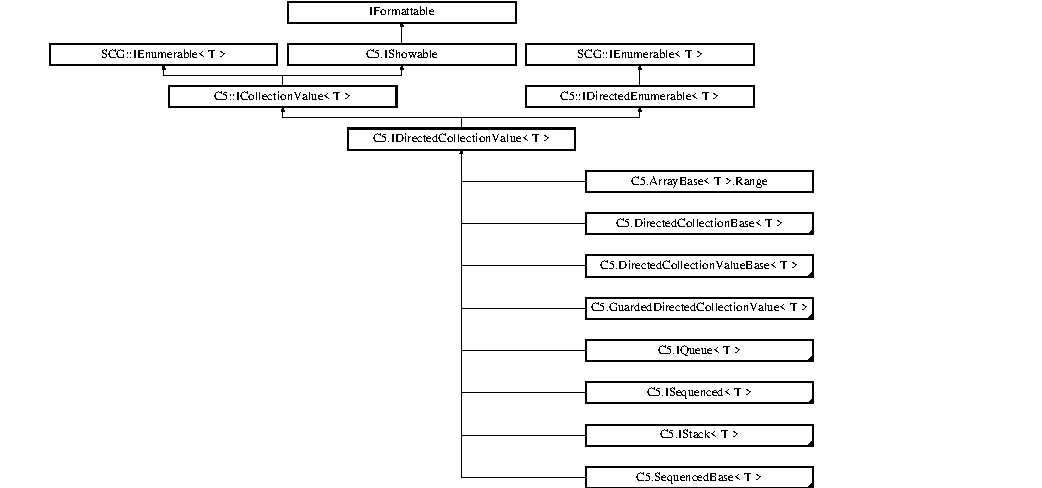
\includegraphics[height=6.536964cm]{interface_c5_1_1_i_directed_collection_value}
\end{center}
\end{figure}
\subsection*{Public Member Functions}
\begin{DoxyCompactItemize}
\item 
new \hyperlink{interface_c5_1_1_i_directed_collection_value}{I\+Directed\+Collection\+Value}$<$ T $>$ \hyperlink{interface_c5_1_1_i_directed_collection_value_ae5665ed396ea2801266c4b2bfb3dae41}{Backwards} ()
\begin{DoxyCompactList}\small\item\em Create a collection containing the same items as this collection, but whose enumerator will enumerate the items backwards. The new collection will become invalid if the original is modified. Method typically used as in \end{DoxyCompactList}\item 
bool \hyperlink{interface_c5_1_1_i_directed_collection_value_a93725b1f694e0d1cf5827e481ea467b7}{Find\+Last} (Func$<$ T, bool $>$ predicate, out T item)
\begin{DoxyCompactList}\small\item\em Check if there exists an item that satisfies a specific predicate in this collection and return the first one in enumeration order. \end{DoxyCompactList}\end{DoxyCompactItemize}
\subsection*{Additional Inherited Members}


\subsection{Detailed Description}
A sized generic collection, that can be enumerated backwards. 



\subsection{Member Function Documentation}
\hypertarget{interface_c5_1_1_i_directed_collection_value_ae5665ed396ea2801266c4b2bfb3dae41}{}\index{C5\+::\+I\+Directed\+Collection\+Value@{C5\+::\+I\+Directed\+Collection\+Value}!Backwards@{Backwards}}
\index{Backwards@{Backwards}!C5\+::\+I\+Directed\+Collection\+Value@{C5\+::\+I\+Directed\+Collection\+Value}}
\subsubsection[{Backwards()}]{\setlength{\rightskip}{0pt plus 5cm}new {\bf I\+Directed\+Collection\+Value}$<$T$>$ {\bf C5.\+I\+Directed\+Collection\+Value}$<$ T $>$.Backwards (
\begin{DoxyParamCaption}
{}
\end{DoxyParamCaption}
)}\label{interface_c5_1_1_i_directed_collection_value_ae5665ed396ea2801266c4b2bfb3dae41}


Create a collection containing the same items as this collection, but whose enumerator will enumerate the items backwards. The new collection will become invalid if the original is modified. Method typically used as in 

{\ttfamily foreach (T x in \hyperlink{namespace_c5_aad282676794e49130eb8caed289395f8a9d1104e419414f4c268be7211fb8fc4a}{coll.\+Backwards()}) \{...\}} 

\begin{DoxyReturn}{Returns}
The backwards collection.
\end{DoxyReturn}


Implements \hyperlink{interface_c5_1_1_i_directed_enumerable_a826d9e7f29272dea7ebd48a38757df9e}{C5.\+I\+Directed\+Enumerable$<$ T $>$}.



Implemented in \hyperlink{class_c5_1_1_tree_bag_aa8d9bd7240bf759fc52c3a14b1f2e43a}{C5.\+Tree\+Bag$<$ T $>$}, \hyperlink{class_c5_1_1_tree_set_a27bc1208dc4fb8e7e1e3be048354ec7b}{C5.\+Tree\+Set$<$ T $>$}, \hyperlink{class_c5_1_1_hashed_linked_list_ad0fbbf15338c5aae4278a5e44f8d9c69}{C5.\+Hashed\+Linked\+List$<$ T $>$}, \hyperlink{class_c5_1_1_linked_list_aa96b744c5e2f0db894b8c9ed9606c240}{C5.\+Linked\+List$<$ T $>$}, \hyperlink{class_c5_1_1_array_base_1_1_range_a296cf1453eb618368fdc14f7abc4f4c2}{C5.\+Array\+Base$<$ T $>$.\+Range}, \hyperlink{class_c5_1_1_array_base_a11fbdc5f71bb41de404f3bd91e3a92b3}{C5.\+Array\+Base$<$ T $>$}, \hyperlink{class_c5_1_1_directed_collection_base_a9a4c7d6571ff7d78ea5adcb0d8264ff1}{C5.\+Directed\+Collection\+Base$<$ T $>$}, \hyperlink{class_c5_1_1_guarded_sequenced_a5bbddf444037001d526931116e6b16e7}{C5.\+Guarded\+Sequenced$<$ T $>$}, \hyperlink{class_c5_1_1_wrapped_array_a2039f22afabd1b152a48ed687dd4e13a}{C5.\+Wrapped\+Array$<$ T $>$}, \hyperlink{class_c5_1_1_directed_collection_value_base_a66d4222e083371d053e609efeecac740}{C5.\+Directed\+Collection\+Value\+Base$<$ T $>$}, \hyperlink{class_c5_1_1_guarded_directed_collection_value_a14e2ad2eb0afbaf5e1ad2e970db81a5b}{C5.\+Guarded\+Directed\+Collection\+Value$<$ T $>$}, and \hyperlink{class_c5_1_1_circular_queue_a9df19a0a07cd854a59df4d3f976cf169}{C5.\+Circular\+Queue$<$ T $>$}.

\hypertarget{interface_c5_1_1_i_directed_collection_value_a93725b1f694e0d1cf5827e481ea467b7}{}\index{C5\+::\+I\+Directed\+Collection\+Value@{C5\+::\+I\+Directed\+Collection\+Value}!Find\+Last@{Find\+Last}}
\index{Find\+Last@{Find\+Last}!C5\+::\+I\+Directed\+Collection\+Value@{C5\+::\+I\+Directed\+Collection\+Value}}
\subsubsection[{Find\+Last(\+Func$<$ T, bool $>$ predicate, out T item)}]{\setlength{\rightskip}{0pt plus 5cm}bool {\bf C5.\+I\+Directed\+Collection\+Value}$<$ T $>$.Find\+Last (
\begin{DoxyParamCaption}
\item[{Func$<$ T, bool $>$}]{predicate, }
\item[{out T}]{item}
\end{DoxyParamCaption}
)}\label{interface_c5_1_1_i_directed_collection_value_a93725b1f694e0d1cf5827e481ea467b7}


Check if there exists an item that satisfies a specific predicate in this collection and return the first one in enumeration order. 


\begin{DoxyParams}{Parameters}
{\em predicate} & A delegate (T\+:\+Func`2 with 
\begin{DoxyCode}
R == \textcolor{keywordtype}{bool}
\end{DoxyCode}
) defining the predicate\\
\hline
{\em item} & \\
\hline
\end{DoxyParams}
\begin{DoxyReturn}{Returns}
True is such an item exists
\end{DoxyReturn}


Implemented in \hyperlink{class_c5_1_1_directed_collection_base_a5dd3482ac69a6ef10092748c9953785b}{C5.\+Directed\+Collection\+Base$<$ T $>$}, \hyperlink{class_c5_1_1_guarded_sequenced_a4741f8cd5c5fa8fb3d6b7a71268cdefb}{C5.\+Guarded\+Sequenced$<$ T $>$}, \hyperlink{class_c5_1_1_wrapped_array_a4917a0c9bba4103b8e63df21b3f9804d}{C5.\+Wrapped\+Array$<$ T $>$}, \hyperlink{class_c5_1_1_directed_collection_value_base_af3d97f14823310f6afd1980d181a4f82}{C5.\+Directed\+Collection\+Value\+Base$<$ T $>$}, and \hyperlink{class_c5_1_1_guarded_directed_collection_value_a755cdf8f197ed79d7616a2b2527d718d}{C5.\+Guarded\+Directed\+Collection\+Value$<$ T $>$}.



The documentation for this interface was generated from the following file\+:\begin{DoxyCompactItemize}
\item 
C\+:/\+Users/rasmusl/\+Source/\+Repos/\+C5/\+C5/\hyperlink{_interfaces_8cs}{Interfaces.\+cs}\end{DoxyCompactItemize}

\hypertarget{interface_c5_1_1_i_directed_enumerable}{}\section{C5.\+I\+Directed\+Enumerable$<$ T $>$ Interface Template Reference}
\label{interface_c5_1_1_i_directed_enumerable}\index{C5.\+I\+Directed\+Enumerable$<$ T $>$@{C5.\+I\+Directed\+Enumerable$<$ T $>$}}


A generic collection, that can be enumerated backwards.  


Inheritance diagram for C5.\+I\+Directed\+Enumerable$<$ T $>$\+:\begin{figure}[H]
\begin{center}
\leavevmode
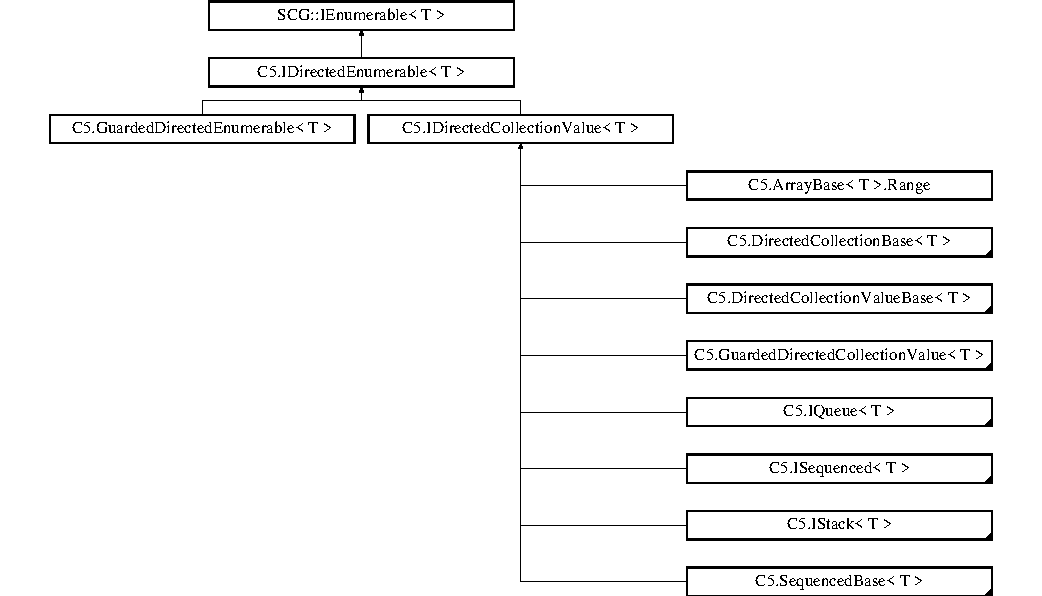
\includegraphics[height=7.989624cm]{interface_c5_1_1_i_directed_enumerable}
\end{center}
\end{figure}
\subsection*{Public Member Functions}
\begin{DoxyCompactItemize}
\item 
\hyperlink{interface_c5_1_1_i_directed_enumerable}{I\+Directed\+Enumerable}$<$ T $>$ \hyperlink{interface_c5_1_1_i_directed_enumerable_a826d9e7f29272dea7ebd48a38757df9e}{Backwards} ()
\begin{DoxyCompactList}\small\item\em Create a collection containing the same items as this collection, but whose enumerator will enumerate the items backwards. The new collection will become invalid if the original is modified. Method typically used as in \end{DoxyCompactList}\end{DoxyCompactItemize}
\subsection*{Properties}
\begin{DoxyCompactItemize}
\item 
\hyperlink{namespace_c5_aad282676794e49130eb8caed289395f8}{Enumeration\+Direction} \hyperlink{interface_c5_1_1_i_directed_enumerable_a4a9d0a85c70671db551d4d0c6efe8564}{Direction}\hspace{0.3cm}{\ttfamily  \mbox{[}get\mbox{]}}
\end{DoxyCompactItemize}


\subsection{Detailed Description}
A generic collection, that can be enumerated backwards. 



\subsection{Member Function Documentation}
\hypertarget{interface_c5_1_1_i_directed_enumerable_a826d9e7f29272dea7ebd48a38757df9e}{}\index{C5\+::\+I\+Directed\+Enumerable@{C5\+::\+I\+Directed\+Enumerable}!Backwards@{Backwards}}
\index{Backwards@{Backwards}!C5\+::\+I\+Directed\+Enumerable@{C5\+::\+I\+Directed\+Enumerable}}
\subsubsection[{Backwards()}]{\setlength{\rightskip}{0pt plus 5cm}{\bf I\+Directed\+Enumerable}$<$T$>$ {\bf C5.\+I\+Directed\+Enumerable}$<$ T $>$.Backwards (
\begin{DoxyParamCaption}
{}
\end{DoxyParamCaption}
)}\label{interface_c5_1_1_i_directed_enumerable_a826d9e7f29272dea7ebd48a38757df9e}


Create a collection containing the same items as this collection, but whose enumerator will enumerate the items backwards. The new collection will become invalid if the original is modified. Method typically used as in 

{\ttfamily foreach (T x in \hyperlink{namespace_c5_aad282676794e49130eb8caed289395f8a9d1104e419414f4c268be7211fb8fc4a}{coll.\+Backwards()}) \{...\}} 

\begin{DoxyReturn}{Returns}
The backwards collection.
\end{DoxyReturn}


Implemented in \hyperlink{class_c5_1_1_tree_bag_aa8d9bd7240bf759fc52c3a14b1f2e43a}{C5.\+Tree\+Bag$<$ T $>$}, \hyperlink{class_c5_1_1_tree_set_a27bc1208dc4fb8e7e1e3be048354ec7b}{C5.\+Tree\+Set$<$ T $>$}, \hyperlink{class_c5_1_1_hashed_linked_list_ad0fbbf15338c5aae4278a5e44f8d9c69}{C5.\+Hashed\+Linked\+List$<$ T $>$}, \hyperlink{class_c5_1_1_linked_list_aa96b744c5e2f0db894b8c9ed9606c240}{C5.\+Linked\+List$<$ T $>$}, \hyperlink{class_c5_1_1_array_base_1_1_range_a296cf1453eb618368fdc14f7abc4f4c2}{C5.\+Array\+Base$<$ T $>$.\+Range}, \hyperlink{class_c5_1_1_array_base_a11fbdc5f71bb41de404f3bd91e3a92b3}{C5.\+Array\+Base$<$ T $>$}, \hyperlink{class_c5_1_1_directed_collection_base_a9a4c7d6571ff7d78ea5adcb0d8264ff1}{C5.\+Directed\+Collection\+Base$<$ T $>$}, \hyperlink{class_c5_1_1_guarded_sequenced_a5bbddf444037001d526931116e6b16e7}{C5.\+Guarded\+Sequenced$<$ T $>$}, \hyperlink{class_c5_1_1_wrapped_array_a2039f22afabd1b152a48ed687dd4e13a}{C5.\+Wrapped\+Array$<$ T $>$}, \hyperlink{class_c5_1_1_directed_collection_value_base_a66d4222e083371d053e609efeecac740}{C5.\+Directed\+Collection\+Value\+Base$<$ T $>$}, \hyperlink{class_c5_1_1_guarded_directed_collection_value_a14e2ad2eb0afbaf5e1ad2e970db81a5b}{C5.\+Guarded\+Directed\+Collection\+Value$<$ T $>$}, \hyperlink{class_c5_1_1_circular_queue_a9df19a0a07cd854a59df4d3f976cf169}{C5.\+Circular\+Queue$<$ T $>$}, \hyperlink{interface_c5_1_1_i_directed_collection_value_ae5665ed396ea2801266c4b2bfb3dae41}{C5.\+I\+Directed\+Collection\+Value$<$ T $>$}, and \hyperlink{class_c5_1_1_guarded_directed_enumerable_a858ca7e55fc0cf083c967e31d9beb8eb}{C5.\+Guarded\+Directed\+Enumerable$<$ T $>$}.



\subsection{Property Documentation}
\hypertarget{interface_c5_1_1_i_directed_enumerable_a4a9d0a85c70671db551d4d0c6efe8564}{}\index{C5\+::\+I\+Directed\+Enumerable@{C5\+::\+I\+Directed\+Enumerable}!Direction@{Direction}}
\index{Direction@{Direction}!C5\+::\+I\+Directed\+Enumerable@{C5\+::\+I\+Directed\+Enumerable}}
\subsubsection[{Direction}]{\setlength{\rightskip}{0pt plus 5cm}{\bf Enumeration\+Direction} {\bf C5.\+I\+Directed\+Enumerable}$<$ T $>$.Direction\hspace{0.3cm}{\ttfamily [get]}}\label{interface_c5_1_1_i_directed_enumerable_a4a9d0a85c70671db551d4d0c6efe8564}




{\ttfamily Forwards} if same, else {\ttfamily Backwards} 

The enumeration direction relative to the original collection.

The documentation for this interface was generated from the following file\+:\begin{DoxyCompactItemize}
\item 
C\+:/\+Users/rasmusl/\+Source/\+Repos/\+C5/\+C5/\hyperlink{_interfaces_8cs}{Interfaces.\+cs}\end{DoxyCompactItemize}

\hypertarget{interface_c5_1_1_i_extensible}{}\section{C5.\+I\+Extensible$<$ T $>$ Interface Template Reference}
\label{interface_c5_1_1_i_extensible}\index{C5.\+I\+Extensible$<$ T $>$@{C5.\+I\+Extensible$<$ T $>$}}


A generic collection to which one may add items. This is just the intersection of the main stream generic collection interfaces and the priority queue interface, T\+:\+C5.\+I\+Collection`1 and T\+:\+C5.\+I\+Priority\+Queue`1.  


Inheritance diagram for C5.\+I\+Extensible$<$ T $>$\+:\begin{figure}[H]
\begin{center}
\leavevmode
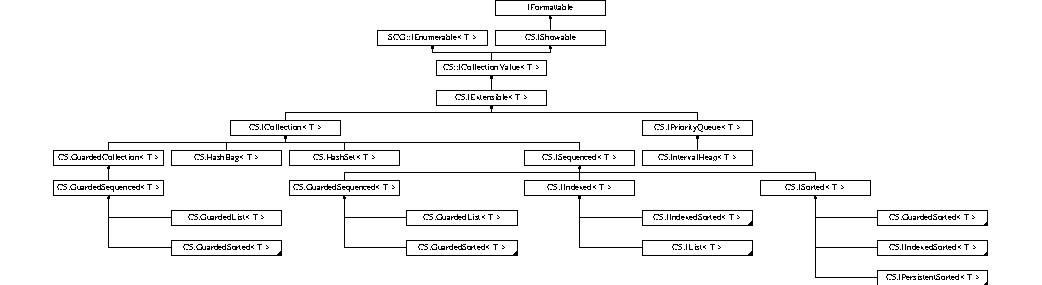
\includegraphics[height=3.825137cm]{interface_c5_1_1_i_extensible}
\end{center}
\end{figure}
\subsection*{Public Member Functions}
\begin{DoxyCompactItemize}
\item 
bool \hyperlink{interface_c5_1_1_i_extensible_acfe8d39605927db1aff0572e2b5c1089}{Add} (T item)
\begin{DoxyCompactList}\small\item\em Add an item to this collection if possible. If this collection has set semantics, the item will be added if not already in the collection. If bag semantics, the item will always be added. \end{DoxyCompactList}\item 
void \hyperlink{interface_c5_1_1_i_extensible_a1fb4d50c5b340e60303da72e9d0ede6e}{Add\+All} (S\+C\+G.\+I\+Enumerable$<$ T $>$ items)
\begin{DoxyCompactList}\small\item\em Add the elements from another collection with a more specialized item type to this collection. If this collection has set semantics, only items not already in the collection will be added. \end{DoxyCompactList}\item 
bool \hyperlink{interface_c5_1_1_i_extensible_aeeb6b87af61e455df42d68834d711bcb}{Check} ()
\begin{DoxyCompactList}\small\item\em Check the integrity of the internal data structures of this collection. {\itshape This is only relevant for developers of the library} \end{DoxyCompactList}\end{DoxyCompactItemize}
\subsection*{Properties}
\begin{DoxyCompactItemize}
\item 
bool \hyperlink{interface_c5_1_1_i_extensible_aedb0e17cd4e5d0f4a63750a5989b6706}{Is\+Read\+Only}\hspace{0.3cm}{\ttfamily  \mbox{[}get\mbox{]}}
\begin{DoxyCompactList}\small\item\em If true any call of an updating operation will throw an \end{DoxyCompactList}\item 
bool \hyperlink{interface_c5_1_1_i_extensible_a1f2129ec206bc1a66e4a62874a67dff7}{Allows\+Duplicates}\hspace{0.3cm}{\ttfamily  \mbox{[}get\mbox{]}}
\item 
S\+C\+G.\+I\+Equality\+Comparer$<$ T $>$ \hyperlink{interface_c5_1_1_i_extensible_a5693514400848e8b544eeffb6deed743}{Equality\+Comparer}\hspace{0.3cm}{\ttfamily  \mbox{[}get\mbox{]}}
\begin{DoxyCompactList}\small\item\em (Here should be a discussion of the role of equality\+Comparers. Any ). \end{DoxyCompactList}\item 
bool \hyperlink{interface_c5_1_1_i_extensible_ae44a9be32f369f1363b64e2c3c682342}{Duplicates\+By\+Counting}\hspace{0.3cm}{\ttfamily  \mbox{[}get\mbox{]}}
\begin{DoxyCompactList}\small\item\em By convention this is true for any collection with set semantics. \end{DoxyCompactList}\end{DoxyCompactItemize}
\subsection*{Additional Inherited Members}


\subsection{Detailed Description}
A generic collection to which one may add items. This is just the intersection of the main stream generic collection interfaces and the priority queue interface, T\+:\+C5.\+I\+Collection`1 and T\+:\+C5.\+I\+Priority\+Queue`1. 



\subsection{Member Function Documentation}
\hypertarget{interface_c5_1_1_i_extensible_acfe8d39605927db1aff0572e2b5c1089}{}\index{C5\+::\+I\+Extensible@{C5\+::\+I\+Extensible}!Add@{Add}}
\index{Add@{Add}!C5\+::\+I\+Extensible@{C5\+::\+I\+Extensible}}
\subsubsection[{Add(\+T item)}]{\setlength{\rightskip}{0pt plus 5cm}bool {\bf C5.\+I\+Extensible}$<$ T $>$.Add (
\begin{DoxyParamCaption}
\item[{T}]{item}
\end{DoxyParamCaption}
)}\label{interface_c5_1_1_i_extensible_acfe8d39605927db1aff0572e2b5c1089}


Add an item to this collection if possible. If this collection has set semantics, the item will be added if not already in the collection. If bag semantics, the item will always be added. 


\begin{DoxyParams}{Parameters}
{\em item} & The item to add.\\
\hline
\end{DoxyParams}
\begin{DoxyReturn}{Returns}
True if item was added.
\end{DoxyReturn}


Implemented in \hyperlink{class_c5_1_1_hashed_linked_list_afcfc7b8da2f00ad7d8e3decadadd74bc}{C5.\+Hashed\+Linked\+List$<$ T $>$}, \hyperlink{class_c5_1_1_linked_list_ac205fdb2cfc336ee2c2843c04fcbad41}{C5.\+Linked\+List$<$ T $>$}, \hyperlink{class_c5_1_1_hashed_array_list_a4606087ab02e09f75ce6810b7a9d11a4}{C5.\+Hashed\+Array\+List$<$ T $>$}, \hyperlink{class_c5_1_1_array_list_a31f07a779aa64ee15f6875ab74682cb5}{C5.\+Array\+List$<$ T $>$}, \hyperlink{class_c5_1_1_sorted_array_a6d4091d5dd1ab9b4637ae16f2bca53e3}{C5.\+Sorted\+Array$<$ T $>$}, \hyperlink{class_c5_1_1_tree_bag_ac407a0824ba7e237c86525234b5b85bd}{C5.\+Tree\+Bag$<$ T $>$}, \hyperlink{class_c5_1_1_tree_set_ae2a3723eb4c1fabdb5b75d52d709f880}{C5.\+Tree\+Set$<$ T $>$}, \hyperlink{interface_c5_1_1_i_list_a800000d7344d000c1b8c67acda464a3d}{C5.\+I\+List$<$ T $>$}, \hyperlink{class_c5_1_1_guarded_collection_aa7fe8941b3b05d9e8622b830852cf12d}{C5.\+Guarded\+Collection$<$ T $>$}, \hyperlink{class_c5_1_1_hash_set_a0700ad4332214ac5d74f3a197bfd8774}{C5.\+Hash\+Set$<$ T $>$}, \hyperlink{class_c5_1_1_wrapped_array_a5be2e0d6422cbc8597e1bc7571b41048}{C5.\+Wrapped\+Array$<$ T $>$}, \hyperlink{class_c5_1_1_hash_bag_a4cc47989ae0d25e5574558f973b85a8d}{C5.\+Hash\+Bag$<$ T $>$}, \hyperlink{class_c5_1_1_interval_heap_ab7c3c348aa1f0f2723dd0a533e1c458f}{C5.\+Interval\+Heap$<$ T $>$}, and \hyperlink{interface_c5_1_1_i_collection_a525115f252ddca586fcbf1a0127be614}{C5.\+I\+Collection$<$ T $>$}.

\hypertarget{interface_c5_1_1_i_extensible_a1fb4d50c5b340e60303da72e9d0ede6e}{}\index{C5\+::\+I\+Extensible@{C5\+::\+I\+Extensible}!Add\+All@{Add\+All}}
\index{Add\+All@{Add\+All}!C5\+::\+I\+Extensible@{C5\+::\+I\+Extensible}}
\subsubsection[{Add\+All(\+S\+C\+G.\+I\+Enumerable$<$ T $>$ items)}]{\setlength{\rightskip}{0pt plus 5cm}void {\bf C5.\+I\+Extensible}$<$ T $>$.Add\+All (
\begin{DoxyParamCaption}
\item[{S\+C\+G.\+I\+Enumerable$<$ T $>$}]{items}
\end{DoxyParamCaption}
)}\label{interface_c5_1_1_i_extensible_a1fb4d50c5b340e60303da72e9d0ede6e}


Add the elements from another collection with a more specialized item type to this collection. If this collection has set semantics, only items not already in the collection will be added. 


\begin{DoxyParams}{Parameters}
{\em items} & The items to add\\
\hline
\end{DoxyParams}


Implemented in \hyperlink{class_c5_1_1_hashed_linked_list_a546555b545da25f99c4ca0e1dc31ddab}{C5.\+Hashed\+Linked\+List$<$ T $>$}, \hyperlink{class_c5_1_1_linked_list_a73d13a68c32ac82f82bed4d8934cc888}{C5.\+Linked\+List$<$ T $>$}, \hyperlink{class_c5_1_1_hashed_array_list_acf2afaacbfe8474425f2840af10118a3}{C5.\+Hashed\+Array\+List$<$ T $>$}, \hyperlink{class_c5_1_1_array_list_ae84250369cc406ec412bc2962acdf9e4}{C5.\+Array\+List$<$ T $>$}, \hyperlink{class_c5_1_1_sorted_array_a0e6b1fe3965a889fc32511d281167ea4}{C5.\+Sorted\+Array$<$ T $>$}, \hyperlink{class_c5_1_1_tree_bag_a12d282c831ea9ef43e39ec92b052729c}{C5.\+Tree\+Bag$<$ T $>$}, \hyperlink{class_c5_1_1_tree_set_a031b4f4a9ad4b680637f865b9f1e255c}{C5.\+Tree\+Set$<$ T $>$}, \hyperlink{class_c5_1_1_hash_set_aabee06dcd4be050a024c507e781d338e}{C5.\+Hash\+Set$<$ T $>$}, \hyperlink{class_c5_1_1_guarded_collection_ac93971d6ad817a2797bf01dbb1d30d12}{C5.\+Guarded\+Collection$<$ T $>$}, \hyperlink{class_c5_1_1_wrapped_array_aaebf1b158171f1848a486e71534e2ef8}{C5.\+Wrapped\+Array$<$ T $>$}, \hyperlink{class_c5_1_1_hash_bag_a87617053c1b6c067efc395b1743e8ed0}{C5.\+Hash\+Bag$<$ T $>$}, and \hyperlink{class_c5_1_1_interval_heap_abe5fb2f06b082e4fec00dc454cd31ed8}{C5.\+Interval\+Heap$<$ T $>$}.

\hypertarget{interface_c5_1_1_i_extensible_aeeb6b87af61e455df42d68834d711bcb}{}\index{C5\+::\+I\+Extensible@{C5\+::\+I\+Extensible}!Check@{Check}}
\index{Check@{Check}!C5\+::\+I\+Extensible@{C5\+::\+I\+Extensible}}
\subsubsection[{Check()}]{\setlength{\rightskip}{0pt plus 5cm}bool {\bf C5.\+I\+Extensible}$<$ T $>$.Check (
\begin{DoxyParamCaption}
{}
\end{DoxyParamCaption}
)}\label{interface_c5_1_1_i_extensible_aeeb6b87af61e455df42d68834d711bcb}


Check the integrity of the internal data structures of this collection. {\itshape This is only relevant for developers of the library} 

\begin{DoxyReturn}{Returns}
True if check was passed.
\end{DoxyReturn}


Implemented in \hyperlink{class_c5_1_1_tree_bag_a6524f8d95ca06232a45aa7c72a43d6cf}{C5.\+Tree\+Bag$<$ T $>$}, \hyperlink{class_c5_1_1_tree_set_a61ffe2a7d9b67271825748d2cefb1274}{C5.\+Tree\+Set$<$ T $>$}, \hyperlink{class_c5_1_1_hashed_linked_list_a03cc4fb3b1f5e3172df5ac12f72167b3}{C5.\+Hashed\+Linked\+List$<$ T $>$}, \hyperlink{class_c5_1_1_linked_list_a9e151b01ae99dd3f5472e0638243e7ec}{C5.\+Linked\+List$<$ T $>$}, \hyperlink{class_c5_1_1_hashed_array_list_aed94ab3e8f52b3cd4b7825b12d6876b2}{C5.\+Hashed\+Array\+List$<$ T $>$}, \hyperlink{class_c5_1_1_array_list_adf389b80c82b6f6164c275e735148eed}{C5.\+Array\+List$<$ T $>$}, \hyperlink{class_c5_1_1_sorted_array_a1b4c759074c4171089f65156607501d4}{C5.\+Sorted\+Array$<$ T $>$}, \hyperlink{class_c5_1_1_hash_set_a7000a1b6fea242f1f5ca40571724b309}{C5.\+Hash\+Set$<$ T $>$}, \hyperlink{class_c5_1_1_guarded_collection_adff17cbe1d82defc187161f1038225fe}{C5.\+Guarded\+Collection$<$ T $>$}, \hyperlink{class_c5_1_1_hash_bag_a19a4c4b0767d7ef9e015bf8b9eadd1e9}{C5.\+Hash\+Bag$<$ T $>$}, \hyperlink{class_c5_1_1_interval_heap_a9682f00247167989ae132c26ded9f600}{C5.\+Interval\+Heap$<$ T $>$}, and \hyperlink{class_c5_1_1_wrapped_array_a9957618a31012883fca40898db85a504}{C5.\+Wrapped\+Array$<$ T $>$}.



\subsection{Property Documentation}
\hypertarget{interface_c5_1_1_i_extensible_a1f2129ec206bc1a66e4a62874a67dff7}{}\index{C5\+::\+I\+Extensible@{C5\+::\+I\+Extensible}!Allows\+Duplicates@{Allows\+Duplicates}}
\index{Allows\+Duplicates@{Allows\+Duplicates}!C5\+::\+I\+Extensible@{C5\+::\+I\+Extensible}}
\subsubsection[{Allows\+Duplicates}]{\setlength{\rightskip}{0pt plus 5cm}bool {\bf C5.\+I\+Extensible}$<$ T $>$.Allows\+Duplicates\hspace{0.3cm}{\ttfamily [get]}}\label{interface_c5_1_1_i_extensible_a1f2129ec206bc1a66e4a62874a67dff7}




False if this collection has set semantics, true if bag semantics.\hypertarget{interface_c5_1_1_i_extensible_ae44a9be32f369f1363b64e2c3c682342}{}\index{C5\+::\+I\+Extensible@{C5\+::\+I\+Extensible}!Duplicates\+By\+Counting@{Duplicates\+By\+Counting}}
\index{Duplicates\+By\+Counting@{Duplicates\+By\+Counting}!C5\+::\+I\+Extensible@{C5\+::\+I\+Extensible}}
\subsubsection[{Duplicates\+By\+Counting}]{\setlength{\rightskip}{0pt plus 5cm}bool {\bf C5.\+I\+Extensible}$<$ T $>$.Duplicates\+By\+Counting\hspace{0.3cm}{\ttfamily [get]}}\label{interface_c5_1_1_i_extensible_ae44a9be32f369f1363b64e2c3c682342}


By convention this is true for any collection with set semantics. 

True if only one representative of a group of equal items is kept in the collection together with the total count.\hypertarget{interface_c5_1_1_i_extensible_a5693514400848e8b544eeffb6deed743}{}\index{C5\+::\+I\+Extensible@{C5\+::\+I\+Extensible}!Equality\+Comparer@{Equality\+Comparer}}
\index{Equality\+Comparer@{Equality\+Comparer}!C5\+::\+I\+Extensible@{C5\+::\+I\+Extensible}}
\subsubsection[{Equality\+Comparer}]{\setlength{\rightskip}{0pt plus 5cm}S\+C\+G.\+I\+Equality\+Comparer$<$T$>$ {\bf C5.\+I\+Extensible}$<$ T $>$.Equality\+Comparer\hspace{0.3cm}{\ttfamily [get]}}\label{interface_c5_1_1_i_extensible_a5693514400848e8b544eeffb6deed743}


(Here should be a discussion of the role of equality\+Comparers. Any ). 

The equality\+Comparer used by this collection to check equality of items. Or null (????) if collection does not check equality at all or uses a comparer.\hypertarget{interface_c5_1_1_i_extensible_aedb0e17cd4e5d0f4a63750a5989b6706}{}\index{C5\+::\+I\+Extensible@{C5\+::\+I\+Extensible}!Is\+Read\+Only@{Is\+Read\+Only}}
\index{Is\+Read\+Only@{Is\+Read\+Only}!C5\+::\+I\+Extensible@{C5\+::\+I\+Extensible}}
\subsubsection[{Is\+Read\+Only}]{\setlength{\rightskip}{0pt plus 5cm}bool {\bf C5.\+I\+Extensible}$<$ T $>$.Is\+Read\+Only\hspace{0.3cm}{\ttfamily [get]}}\label{interface_c5_1_1_i_extensible_aedb0e17cd4e5d0f4a63750a5989b6706}


If true any call of an updating operation will throw an 

{\ttfamily \hyperlink{class_c5_1_1_read_only_collection_exception}{Read\+Only\+Collection\+Exception}} 

True if this collection is read-\/only.

The documentation for this interface was generated from the following file\+:\begin{DoxyCompactItemize}
\item 
C\+:/\+Users/rasmusl/\+Source/\+Repos/\+C5/\+C5/\hyperlink{_interfaces_8cs}{Interfaces.\+cs}\end{DoxyCompactItemize}

\hypertarget{interface_c5_1_1_i_indexed}{}\section{C5.\+I\+Indexed$<$ T $>$ Interface Template Reference}
\label{interface_c5_1_1_i_indexed}\index{C5.\+I\+Indexed$<$ T $>$@{C5.\+I\+Indexed$<$ T $>$}}


A sequenced collection, where indices of items in the order are maintained  


Inheritance diagram for C5.\+I\+Indexed$<$ T $>$\+:\begin{figure}[H]
\begin{center}
\leavevmode
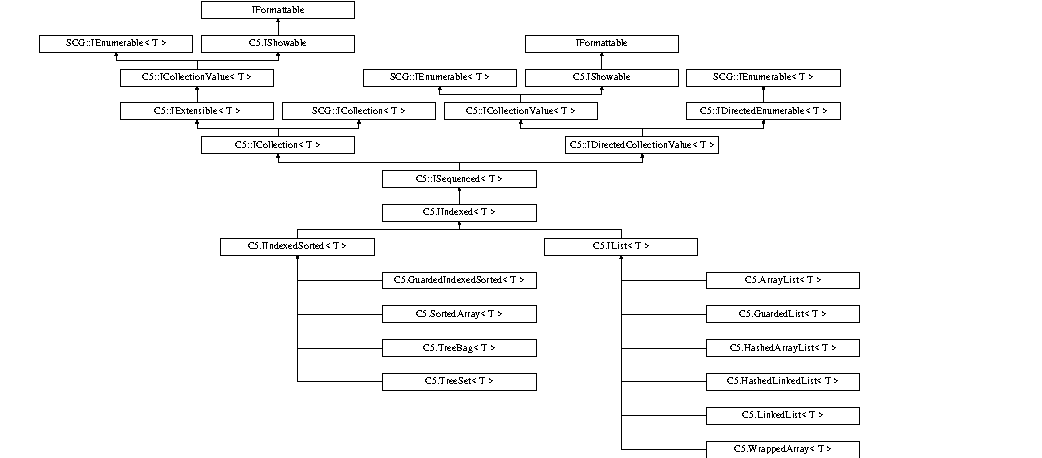
\includegraphics[height=6.134585cm]{interface_c5_1_1_i_indexed}
\end{center}
\end{figure}
\subsection*{Public Member Functions}
\begin{DoxyCompactItemize}
\item 
int \hyperlink{interface_c5_1_1_i_indexed_abad58598415e0383ddbc9275db69d92a}{Index\+Of} (T item)
\begin{DoxyCompactList}\small\item\em Searches for an item in the list going forwards from the start. \end{DoxyCompactList}\item 
int \hyperlink{interface_c5_1_1_i_indexed_a50f274e0f7b4cd2e54db4cb61a003b95}{Last\+Index\+Of} (T item)
\begin{DoxyCompactList}\small\item\em Searches for an item in the list going backwards from the end. \end{DoxyCompactList}\item 
int \hyperlink{interface_c5_1_1_i_indexed_ac5431f5a857165b38d36b066d17e288c}{Find\+Index} (Func$<$ T, bool $>$ predicate)
\begin{DoxyCompactList}\small\item\em Check if there exists an item that satisfies a specific predicate in this collection and return the index of the first one. \end{DoxyCompactList}\item 
int \hyperlink{interface_c5_1_1_i_indexed_a4283e602a819d8ea03d1af10983b5105}{Find\+Last\+Index} (Func$<$ T, bool $>$ predicate)
\begin{DoxyCompactList}\small\item\em Check if there exists an item that satisfies a specific predicate in this collection and return the index of the last one. \end{DoxyCompactList}\item 
T \hyperlink{interface_c5_1_1_i_indexed_ac741e6d3d7c6a30bb8a013bb29591ca4}{Remove\+At} (int index)
\begin{DoxyCompactList}\small\item\em Remove the item at a specific position of the list. \end{DoxyCompactList}\item 
void \hyperlink{interface_c5_1_1_i_indexed_aa9d2a1706ba0361079d31c02bad3e810}{Remove\+Interval} (int start, int count)
\begin{DoxyCompactList}\small\item\em Remove all items in an index interval. \end{DoxyCompactList}\end{DoxyCompactItemize}
\subsection*{Properties}
\begin{DoxyCompactItemize}
\item 
T \hyperlink{interface_c5_1_1_i_indexed_a1e716eed0c1bc5b1d30e456fab869dc6}{this\mbox{[}int index\mbox{]}}\hspace{0.3cm}{\ttfamily  \mbox{[}get\mbox{]}}
\item 
\hyperlink{namespace_c5_a615ba88dcdaa8d5a3c5f833a73d7fad6}{Speed} \hyperlink{interface_c5_1_1_i_indexed_a32f84a737f8725bc93ff50b44539a413}{Indexing\+Speed}\hspace{0.3cm}{\ttfamily  \mbox{[}get\mbox{]}}
\item 
\hyperlink{interface_c5_1_1_i_directed_collection_value}{I\+Directed\+Collection\+Value}$<$ T $>$ \hyperlink{interface_c5_1_1_i_indexed_a7d2ebaba4aefbc5240fb95893596337a}{this\mbox{[}int start, int count\mbox{]}}\hspace{0.3cm}{\ttfamily  \mbox{[}get\mbox{]}}
\end{DoxyCompactItemize}
\subsection*{Additional Inherited Members}


\subsection{Detailed Description}
A sequenced collection, where indices of items in the order are maintained 



\subsection{Member Function Documentation}
\hypertarget{interface_c5_1_1_i_indexed_ac5431f5a857165b38d36b066d17e288c}{}\index{C5\+::\+I\+Indexed@{C5\+::\+I\+Indexed}!Find\+Index@{Find\+Index}}
\index{Find\+Index@{Find\+Index}!C5\+::\+I\+Indexed@{C5\+::\+I\+Indexed}}
\subsubsection[{Find\+Index(\+Func$<$ T, bool $>$ predicate)}]{\setlength{\rightskip}{0pt plus 5cm}int {\bf C5.\+I\+Indexed}$<$ T $>$.Find\+Index (
\begin{DoxyParamCaption}
\item[{Func$<$ T, bool $>$}]{predicate}
\end{DoxyParamCaption}
)}\label{interface_c5_1_1_i_indexed_ac5431f5a857165b38d36b066d17e288c}


Check if there exists an item that satisfies a specific predicate in this collection and return the index of the first one. 


\begin{DoxyParams}{Parameters}
{\em predicate} & A delegate (T\+:\+Func`2 with 
\begin{DoxyCode}
R == \textcolor{keywordtype}{bool}
\end{DoxyCode}
) defining the predicate\\
\hline
\end{DoxyParams}
\begin{DoxyReturn}{Returns}
the index, if found, a negative value else
\end{DoxyReturn}


Implemented in \hyperlink{class_c5_1_1_wrapped_array_a189ddcea1c7463ce3e8899e2709614d5}{C5.\+Wrapped\+Array$<$ T $>$}.

\hypertarget{interface_c5_1_1_i_indexed_a4283e602a819d8ea03d1af10983b5105}{}\index{C5\+::\+I\+Indexed@{C5\+::\+I\+Indexed}!Find\+Last\+Index@{Find\+Last\+Index}}
\index{Find\+Last\+Index@{Find\+Last\+Index}!C5\+::\+I\+Indexed@{C5\+::\+I\+Indexed}}
\subsubsection[{Find\+Last\+Index(\+Func$<$ T, bool $>$ predicate)}]{\setlength{\rightskip}{0pt plus 5cm}int {\bf C5.\+I\+Indexed}$<$ T $>$.Find\+Last\+Index (
\begin{DoxyParamCaption}
\item[{Func$<$ T, bool $>$}]{predicate}
\end{DoxyParamCaption}
)}\label{interface_c5_1_1_i_indexed_a4283e602a819d8ea03d1af10983b5105}


Check if there exists an item that satisfies a specific predicate in this collection and return the index of the last one. 


\begin{DoxyParams}{Parameters}
{\em predicate} & A delegate (T\+:\+Func`2 with 
\begin{DoxyCode}
R == \textcolor{keywordtype}{bool}
\end{DoxyCode}
) defining the predicate\\
\hline
\end{DoxyParams}
\begin{DoxyReturn}{Returns}
the index, if found, a negative value else
\end{DoxyReturn}


Implemented in \hyperlink{class_c5_1_1_wrapped_array_a7606c974ca7844dbbab61e0671f72a53}{C5.\+Wrapped\+Array$<$ T $>$}.

\hypertarget{interface_c5_1_1_i_indexed_abad58598415e0383ddbc9275db69d92a}{}\index{C5\+::\+I\+Indexed@{C5\+::\+I\+Indexed}!Index\+Of@{Index\+Of}}
\index{Index\+Of@{Index\+Of}!C5\+::\+I\+Indexed@{C5\+::\+I\+Indexed}}
\subsubsection[{Index\+Of(\+T item)}]{\setlength{\rightskip}{0pt plus 5cm}int {\bf C5.\+I\+Indexed}$<$ T $>$.Index\+Of (
\begin{DoxyParamCaption}
\item[{T}]{item}
\end{DoxyParamCaption}
)}\label{interface_c5_1_1_i_indexed_abad58598415e0383ddbc9275db69d92a}


Searches for an item in the list going forwards from the start. 


\begin{DoxyParams}{Parameters}
{\em item} & Item to search for.\\
\hline
\end{DoxyParams}
\begin{DoxyReturn}{Returns}
Index of item from start. A negative number if item not found, namely the one\textquotesingle{}s complement of the index at which the Add operation would put the item.
\end{DoxyReturn}


Implemented in \hyperlink{class_c5_1_1_tree_bag_ae70bb012099ffac0759c74b589fb811a}{C5.\+Tree\+Bag$<$ T $>$}, \hyperlink{class_c5_1_1_tree_set_a9a7af62e8459c31c03f984e84851ffb9}{C5.\+Tree\+Set$<$ T $>$}, \hyperlink{class_c5_1_1_hashed_linked_list_aca8634364d0bfec4b0d2bb8b7c6f5c98}{C5.\+Hashed\+Linked\+List$<$ T $>$}, \hyperlink{class_c5_1_1_guarded_list_aac2b7de89c7556b8a1c0b49dad25174f}{C5.\+Guarded\+List$<$ T $>$}, \hyperlink{class_c5_1_1_linked_list_a4dc305430081a02d96b65c285a61be7b}{C5.\+Linked\+List$<$ T $>$}, \hyperlink{class_c5_1_1_sorted_array_a20a6a1e7bead68d88ab599abb8aff039}{C5.\+Sorted\+Array$<$ T $>$}, \hyperlink{class_c5_1_1_hashed_array_list_a6d13105e7f303fc04310801abed22946}{C5.\+Hashed\+Array\+List$<$ T $>$}, \hyperlink{class_c5_1_1_array_list_ae94dff251b125331c450b396418bb1be}{C5.\+Array\+List$<$ T $>$}, \hyperlink{class_c5_1_1_guarded_indexed_sorted_aa13e57faa854dd70f28ac2dd8bb6f888}{C5.\+Guarded\+Indexed\+Sorted$<$ T $>$}, \hyperlink{interface_c5_1_1_i_list_a52658ee618f1557622d766d7a348910a}{C5.\+I\+List$<$ T $>$}, and \hyperlink{class_c5_1_1_wrapped_array_a459af83c432f3dbc167d406c4632fb0e}{C5.\+Wrapped\+Array$<$ T $>$}.

\hypertarget{interface_c5_1_1_i_indexed_a50f274e0f7b4cd2e54db4cb61a003b95}{}\index{C5\+::\+I\+Indexed@{C5\+::\+I\+Indexed}!Last\+Index\+Of@{Last\+Index\+Of}}
\index{Last\+Index\+Of@{Last\+Index\+Of}!C5\+::\+I\+Indexed@{C5\+::\+I\+Indexed}}
\subsubsection[{Last\+Index\+Of(\+T item)}]{\setlength{\rightskip}{0pt plus 5cm}int {\bf C5.\+I\+Indexed}$<$ T $>$.Last\+Index\+Of (
\begin{DoxyParamCaption}
\item[{T}]{item}
\end{DoxyParamCaption}
)}\label{interface_c5_1_1_i_indexed_a50f274e0f7b4cd2e54db4cb61a003b95}


Searches for an item in the list going backwards from the end. 


\begin{DoxyParams}{Parameters}
{\em item} & Item to search for.\\
\hline
\end{DoxyParams}
\begin{DoxyReturn}{Returns}
Index of of item from the end. A negative number if item not found, namely the two-\/complement of the index at which the Add operation would put the item.
\end{DoxyReturn}


Implemented in \hyperlink{class_c5_1_1_tree_bag_ad51c9faeac6e8262b8cfbb6baeba23d4}{C5.\+Tree\+Bag$<$ T $>$}, \hyperlink{class_c5_1_1_tree_set_a099dbba4e62506b221780172c30e84ce}{C5.\+Tree\+Set$<$ T $>$}, \hyperlink{class_c5_1_1_hashed_linked_list_a4e053c03fa87e356bab7ec25a529607a}{C5.\+Hashed\+Linked\+List$<$ T $>$}, \hyperlink{class_c5_1_1_guarded_list_a6813134b41bdb0f98b473f02800809c2}{C5.\+Guarded\+List$<$ T $>$}, \hyperlink{class_c5_1_1_linked_list_a0a4631db1f533e2561511edf9f4858b9}{C5.\+Linked\+List$<$ T $>$}, \hyperlink{class_c5_1_1_sorted_array_a1989414a3df7eaabc5ec2ff36f3f613e}{C5.\+Sorted\+Array$<$ T $>$}, \hyperlink{class_c5_1_1_hashed_array_list_a6fff76a2253ec4f3fb52abcddecbc52c}{C5.\+Hashed\+Array\+List$<$ T $>$}, \hyperlink{class_c5_1_1_array_list_af04d77e11483bfcfa1cac7fd88b57bc5}{C5.\+Array\+List$<$ T $>$}, \hyperlink{class_c5_1_1_guarded_indexed_sorted_a782d9e939a68f246af69adba83584164}{C5.\+Guarded\+Indexed\+Sorted$<$ T $>$}, and \hyperlink{class_c5_1_1_wrapped_array_aebda540a1e886890698d527f53d99343}{C5.\+Wrapped\+Array$<$ T $>$}.

\hypertarget{interface_c5_1_1_i_indexed_ac741e6d3d7c6a30bb8a013bb29591ca4}{}\index{C5\+::\+I\+Indexed@{C5\+::\+I\+Indexed}!Remove\+At@{Remove\+At}}
\index{Remove\+At@{Remove\+At}!C5\+::\+I\+Indexed@{C5\+::\+I\+Indexed}}
\subsubsection[{Remove\+At(int index)}]{\setlength{\rightskip}{0pt plus 5cm}T {\bf C5.\+I\+Indexed}$<$ T $>$.Remove\+At (
\begin{DoxyParamCaption}
\item[{int}]{index}
\end{DoxyParamCaption}
)}\label{interface_c5_1_1_i_indexed_ac741e6d3d7c6a30bb8a013bb29591ca4}


Remove the item at a specific position of the list. 


\begin{DoxyExceptions}{Exceptions}
{\em Index\+Out\+Of\+Range\+Exception} & if 
\begin{DoxyCode}
index
\end{DoxyCode}
 is negative or $>$= the size of the collection.\\
\hline
\end{DoxyExceptions}

\begin{DoxyParams}{Parameters}
{\em index} & The index of the item to remove.\\
\hline
\end{DoxyParams}
\begin{DoxyReturn}{Returns}
The removed item.
\end{DoxyReturn}


Implemented in \hyperlink{class_c5_1_1_tree_bag_afe0ad1fba513ec3b14e73e457230d87d}{C5.\+Tree\+Bag$<$ T $>$}, \hyperlink{class_c5_1_1_tree_set_aa12a3942109e24ea3ebbf22238af8f78}{C5.\+Tree\+Set$<$ T $>$}, \hyperlink{class_c5_1_1_hashed_linked_list_ae29691247778dcae44ae4a4482c4c94f}{C5.\+Hashed\+Linked\+List$<$ T $>$}, \hyperlink{class_c5_1_1_guarded_list_a051deb35bed74f188be08a40c1e79afa}{C5.\+Guarded\+List$<$ T $>$}, \hyperlink{class_c5_1_1_linked_list_ad5bcb57accd6b97265cf8c12efeda71c}{C5.\+Linked\+List$<$ T $>$}, \hyperlink{class_c5_1_1_sorted_array_a901cec8ac5a0a876476285ae7dd3e7e2}{C5.\+Sorted\+Array$<$ T $>$}, \hyperlink{class_c5_1_1_hashed_array_list_a28dadd5b31e5daa8eb34728f0c31728a}{C5.\+Hashed\+Array\+List$<$ T $>$}, \hyperlink{class_c5_1_1_array_list_a0f3b4828a1c3ba06d035ad6f2aa491fc}{C5.\+Array\+List$<$ T $>$}, \hyperlink{class_c5_1_1_guarded_indexed_sorted_a0e84a6bb3bf610cdf68aa2583dc78155}{C5.\+Guarded\+Indexed\+Sorted$<$ T $>$}, \hyperlink{interface_c5_1_1_i_list_a9fbcd9c55aae61134321939d0b104cc0}{C5.\+I\+List$<$ T $>$}, and \hyperlink{class_c5_1_1_wrapped_array_a01b30a7260874fcd043d01cabad29f55}{C5.\+Wrapped\+Array$<$ T $>$}.

\hypertarget{interface_c5_1_1_i_indexed_aa9d2a1706ba0361079d31c02bad3e810}{}\index{C5\+::\+I\+Indexed@{C5\+::\+I\+Indexed}!Remove\+Interval@{Remove\+Interval}}
\index{Remove\+Interval@{Remove\+Interval}!C5\+::\+I\+Indexed@{C5\+::\+I\+Indexed}}
\subsubsection[{Remove\+Interval(int start, int count)}]{\setlength{\rightskip}{0pt plus 5cm}void {\bf C5.\+I\+Indexed}$<$ T $>$.Remove\+Interval (
\begin{DoxyParamCaption}
\item[{int}]{start, }
\item[{int}]{count}
\end{DoxyParamCaption}
)}\label{interface_c5_1_1_i_indexed_aa9d2a1706ba0361079d31c02bad3e810}


Remove all items in an index interval. 


\begin{DoxyExceptions}{Exceptions}
{\em Argument\+Out\+Of\+Range\+Exception} & if start or count is negative or start+count $>$ the size of the collection.\\
\hline
\end{DoxyExceptions}

\begin{DoxyParams}{Parameters}
{\em start} & The index of the first item to remove.\\
\hline
{\em count} & The number of items to remove.\\
\hline
\end{DoxyParams}


Implemented in \hyperlink{class_c5_1_1_tree_bag_af77f6e665a61d88fa0ed881a66984601}{C5.\+Tree\+Bag$<$ T $>$}, \hyperlink{class_c5_1_1_tree_set_a23b614ca0fa47fa4971088c40998bf5e}{C5.\+Tree\+Set$<$ T $>$}, \hyperlink{class_c5_1_1_hashed_linked_list_ab2b43feeeb2c5cece0d5e65949c178b3}{C5.\+Hashed\+Linked\+List$<$ T $>$}, \hyperlink{class_c5_1_1_guarded_list_addc4ab1ca7eb4bf0daebf4453d1397e5}{C5.\+Guarded\+List$<$ T $>$}, \hyperlink{class_c5_1_1_linked_list_a6deeac14ff0d6c8d9a498d8f609501a5}{C5.\+Linked\+List$<$ T $>$}, \hyperlink{class_c5_1_1_sorted_array_a277e0cf59b483ba0378d6ec0f240ecef}{C5.\+Sorted\+Array$<$ T $>$}, \hyperlink{class_c5_1_1_hashed_array_list_ab443d1ea4dd141b18debf8d450deb2fb}{C5.\+Hashed\+Array\+List$<$ T $>$}, \hyperlink{class_c5_1_1_array_list_aa4c6f08712ec985076e402d713e5a616}{C5.\+Array\+List$<$ T $>$}, \hyperlink{class_c5_1_1_guarded_indexed_sorted_a2c43f17a32750da03b1aa64a6300a091}{C5.\+Guarded\+Indexed\+Sorted$<$ T $>$}, and \hyperlink{class_c5_1_1_wrapped_array_ae488079bb94b8ed0bdb0ce834ec2dd25}{C5.\+Wrapped\+Array$<$ T $>$}.



\subsection{Property Documentation}
\hypertarget{interface_c5_1_1_i_indexed_a32f84a737f8725bc93ff50b44539a413}{}\index{C5\+::\+I\+Indexed@{C5\+::\+I\+Indexed}!Indexing\+Speed@{Indexing\+Speed}}
\index{Indexing\+Speed@{Indexing\+Speed}!C5\+::\+I\+Indexed@{C5\+::\+I\+Indexed}}
\subsubsection[{Indexing\+Speed}]{\setlength{\rightskip}{0pt plus 5cm}{\bf Speed} {\bf C5.\+I\+Indexed}$<$ T $>$.Indexing\+Speed\hspace{0.3cm}{\ttfamily [get]}}\label{interface_c5_1_1_i_indexed_a32f84a737f8725bc93ff50b44539a413}




\hypertarget{interface_c5_1_1_i_indexed_a1e716eed0c1bc5b1d30e456fab869dc6}{}\index{C5\+::\+I\+Indexed@{C5\+::\+I\+Indexed}!this\mbox{[}int index\mbox{]}@{this[int index]}}
\index{this\mbox{[}int index\mbox{]}@{this[int index]}!C5\+::\+I\+Indexed@{C5\+::\+I\+Indexed}}
\subsubsection[{this[int index]}]{\setlength{\rightskip}{0pt plus 5cm}T {\bf C5.\+I\+Indexed}$<$ T $>$.this\mbox{[}int index\mbox{]}\hspace{0.3cm}{\ttfamily [get]}}\label{interface_c5_1_1_i_indexed_a1e716eed0c1bc5b1d30e456fab869dc6}





\begin{DoxyExceptions}{Exceptions}
{\em Index\+Out\+Of\+Range\+Exception} & if 
\begin{DoxyCode}
index
\end{DoxyCode}
 is negative or $>$= the size of the collection.\\
\hline
\end{DoxyExceptions}


The 
\begin{DoxyCode}
index
\end{DoxyCode}
\textquotesingle{}th item of this list.


\begin{DoxyParams}{Parameters}
{\em index} & the index to lookup\\
\hline
\end{DoxyParams}
\hypertarget{interface_c5_1_1_i_indexed_a7d2ebaba4aefbc5240fb95893596337a}{}\index{C5\+::\+I\+Indexed@{C5\+::\+I\+Indexed}!this\mbox{[}int start, int count\mbox{]}@{this[int start, int count]}}
\index{this\mbox{[}int start, int count\mbox{]}@{this[int start, int count]}!C5\+::\+I\+Indexed@{C5\+::\+I\+Indexed}}
\subsubsection[{this[int start, int count]}]{\setlength{\rightskip}{0pt plus 5cm}{\bf I\+Directed\+Collection\+Value}$<$T$>$ {\bf C5.\+I\+Indexed}$<$ T $>$.this\mbox{[}int start, int count\mbox{]}\hspace{0.3cm}{\ttfamily [get]}}\label{interface_c5_1_1_i_indexed_a7d2ebaba4aefbc5240fb95893596337a}





\begin{DoxyExceptions}{Exceptions}
{\em Argument\+Out\+Of\+Range\+Exception} & \\
\hline
\end{DoxyExceptions}


The directed collection of items in a specific index interval.


\begin{DoxyParams}{Parameters}
{\em start} & The low index of the interval (inclusive).\\
\hline
{\em count} & The size of the range.\\
\hline
\end{DoxyParams}


The documentation for this interface was generated from the following file\+:\begin{DoxyCompactItemize}
\item 
C\+:/\+Users/rasmusl/\+Source/\+Repos/\+C5/\+C5/\hyperlink{_interfaces_8cs}{Interfaces.\+cs}\end{DoxyCompactItemize}

\hypertarget{interface_c5_1_1_i_indexed_sorted}{}\section{C5.\+I\+Indexed\+Sorted$<$ T $>$ Interface Template Reference}
\label{interface_c5_1_1_i_indexed_sorted}\index{C5.\+I\+Indexed\+Sorted$<$ T $>$@{C5.\+I\+Indexed\+Sorted$<$ T $>$}}


A collection where items are maintained in sorted order together with their indexes in that order.  


Inheritance diagram for C5.\+I\+Indexed\+Sorted$<$ T $>$\+:\begin{figure}[H]
\begin{center}
\leavevmode
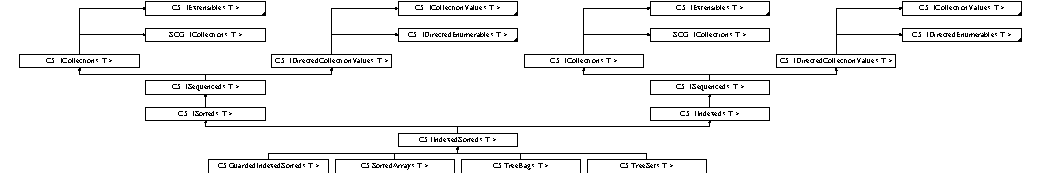
\includegraphics[height=2.300470cm]{interface_c5_1_1_i_indexed_sorted}
\end{center}
\end{figure}
\subsection*{Public Member Functions}
\begin{DoxyCompactItemize}
\item 
int \hyperlink{interface_c5_1_1_i_indexed_sorted_afec472803ce8298d60dfc5dfb2f8f925}{Count\+From} (T bot)
\begin{DoxyCompactList}\small\item\em Determine the number of items at or above a supplied threshold. \end{DoxyCompactList}\item 
int \hyperlink{interface_c5_1_1_i_indexed_sorted_a6b8dd3c5325621b9a81a7e5167328773}{Count\+From\+To} (T bot, T top)
\begin{DoxyCompactList}\small\item\em Determine the number of items between two supplied thresholds. \end{DoxyCompactList}\item 
int \hyperlink{interface_c5_1_1_i_indexed_sorted_ae69946df07200b99fa1336681223680a}{Count\+To} (T top)
\begin{DoxyCompactList}\small\item\em Determine the number of items below a supplied threshold. \end{DoxyCompactList}\item 
new \hyperlink{interface_c5_1_1_i_directed_collection_value}{I\+Directed\+Collection\+Value}$<$ T $>$ \hyperlink{interface_c5_1_1_i_indexed_sorted_a798fe33ccf02cdb90e7966bf73d100eb}{Range\+From} (T bot)
\begin{DoxyCompactList}\small\item\em Query this sorted collection for items greater than or equal to a supplied value. \end{DoxyCompactList}\item 
new \hyperlink{interface_c5_1_1_i_directed_collection_value}{I\+Directed\+Collection\+Value}$<$ T $>$ \hyperlink{interface_c5_1_1_i_indexed_sorted_a7fd04b75c6f1e86867f8a27309067a5d}{Range\+From\+To} (T bot, T top)
\begin{DoxyCompactList}\small\item\em Query this sorted collection for items between two supplied values. \end{DoxyCompactList}\item 
new \hyperlink{interface_c5_1_1_i_directed_collection_value}{I\+Directed\+Collection\+Value}$<$ T $>$ \hyperlink{interface_c5_1_1_i_indexed_sorted_a62820d898864d45d9029d9df06ab3c5d}{Range\+To} (T top)
\begin{DoxyCompactList}\small\item\em Query this sorted collection for items less than a supplied value. \end{DoxyCompactList}\item 
\hyperlink{interface_c5_1_1_i_indexed_sorted}{I\+Indexed\+Sorted}$<$ T $>$ \hyperlink{interface_c5_1_1_i_indexed_sorted_a0919e5cb5b659d0de7c206a3c3bc033d}{Find\+All} (Func$<$ T, bool $>$ predicate)
\begin{DoxyCompactList}\small\item\em Create a new indexed sorted collection consisting of the items of this indexed sorted collection satisfying a certain predicate. \end{DoxyCompactList}\item 
\hyperlink{interface_c5_1_1_i_indexed_sorted}{I\+Indexed\+Sorted}$<$ V $>$ \hyperlink{interface_c5_1_1_i_indexed_sorted_ab895a7e04cffcc97f6f0ef5e7c00b171}{Map$<$ V $>$} (Func$<$ T, V $>$ mapper, S\+C\+G.\+I\+Comparer$<$ V $>$ comparer)
\begin{DoxyCompactList}\small\item\em Create a new indexed sorted collection consisting of the results of mapping all items of this list. 
\begin{DoxyExceptions}{Exceptions}
{\em Argument\+Exception} & if the map is not increasing over the items of this collection (with respect to the two given comparison relations). \\
\hline
\end{DoxyExceptions}
\end{DoxyCompactList}\end{DoxyCompactItemize}
\subsection*{Additional Inherited Members}


\subsection{Detailed Description}
A collection where items are maintained in sorted order together with their indexes in that order. 



\subsection{Member Function Documentation}
\hypertarget{interface_c5_1_1_i_indexed_sorted_afec472803ce8298d60dfc5dfb2f8f925}{}\index{C5\+::\+I\+Indexed\+Sorted@{C5\+::\+I\+Indexed\+Sorted}!Count\+From@{Count\+From}}
\index{Count\+From@{Count\+From}!C5\+::\+I\+Indexed\+Sorted@{C5\+::\+I\+Indexed\+Sorted}}
\subsubsection[{Count\+From(\+T bot)}]{\setlength{\rightskip}{0pt plus 5cm}int {\bf C5.\+I\+Indexed\+Sorted}$<$ T $>$.Count\+From (
\begin{DoxyParamCaption}
\item[{T}]{bot}
\end{DoxyParamCaption}
)}\label{interface_c5_1_1_i_indexed_sorted_afec472803ce8298d60dfc5dfb2f8f925}


Determine the number of items at or above a supplied threshold. 


\begin{DoxyParams}{Parameters}
{\em bot} & The lower bound (inclusive)\\
\hline
\end{DoxyParams}
\begin{DoxyReturn}{Returns}
The number of matcing items.
\end{DoxyReturn}


Implemented in \hyperlink{class_c5_1_1_tree_bag_a5fbb54d05147aad25ba53f3102f68d8b}{C5.\+Tree\+Bag$<$ T $>$}, \hyperlink{class_c5_1_1_tree_set_a9572f2d67981336f00d0146aa8a28b33}{C5.\+Tree\+Set$<$ T $>$}, \hyperlink{class_c5_1_1_guarded_indexed_sorted_a8cf3d09d8c435ac0200efc34561e1a86}{C5.\+Guarded\+Indexed\+Sorted$<$ T $>$}, and \hyperlink{class_c5_1_1_sorted_array_a7249ec52c01564107e7825c1e81e0761}{C5.\+Sorted\+Array$<$ T $>$}.

\hypertarget{interface_c5_1_1_i_indexed_sorted_a6b8dd3c5325621b9a81a7e5167328773}{}\index{C5\+::\+I\+Indexed\+Sorted@{C5\+::\+I\+Indexed\+Sorted}!Count\+From\+To@{Count\+From\+To}}
\index{Count\+From\+To@{Count\+From\+To}!C5\+::\+I\+Indexed\+Sorted@{C5\+::\+I\+Indexed\+Sorted}}
\subsubsection[{Count\+From\+To(\+T bot, T top)}]{\setlength{\rightskip}{0pt plus 5cm}int {\bf C5.\+I\+Indexed\+Sorted}$<$ T $>$.Count\+From\+To (
\begin{DoxyParamCaption}
\item[{T}]{bot, }
\item[{T}]{top}
\end{DoxyParamCaption}
)}\label{interface_c5_1_1_i_indexed_sorted_a6b8dd3c5325621b9a81a7e5167328773}


Determine the number of items between two supplied thresholds. 


\begin{DoxyParams}{Parameters}
{\em bot} & The lower bound (inclusive)\\
\hline
{\em top} & The upper bound (exclusive)\\
\hline
\end{DoxyParams}
\begin{DoxyReturn}{Returns}
The number of matcing items.
\end{DoxyReturn}


Implemented in \hyperlink{class_c5_1_1_tree_bag_a4ee93d234390b558f6566446502fd2d8}{C5.\+Tree\+Bag$<$ T $>$}, \hyperlink{class_c5_1_1_tree_set_a1e7a0e1964ad077bab826f4946c03838}{C5.\+Tree\+Set$<$ T $>$}, \hyperlink{class_c5_1_1_guarded_indexed_sorted_af8a01e371525dfae61ddc323e16e1f9e}{C5.\+Guarded\+Indexed\+Sorted$<$ T $>$}, and \hyperlink{class_c5_1_1_sorted_array_a28de6027688415f83909e0460616b87a}{C5.\+Sorted\+Array$<$ T $>$}.

\hypertarget{interface_c5_1_1_i_indexed_sorted_ae69946df07200b99fa1336681223680a}{}\index{C5\+::\+I\+Indexed\+Sorted@{C5\+::\+I\+Indexed\+Sorted}!Count\+To@{Count\+To}}
\index{Count\+To@{Count\+To}!C5\+::\+I\+Indexed\+Sorted@{C5\+::\+I\+Indexed\+Sorted}}
\subsubsection[{Count\+To(\+T top)}]{\setlength{\rightskip}{0pt plus 5cm}int {\bf C5.\+I\+Indexed\+Sorted}$<$ T $>$.Count\+To (
\begin{DoxyParamCaption}
\item[{T}]{top}
\end{DoxyParamCaption}
)}\label{interface_c5_1_1_i_indexed_sorted_ae69946df07200b99fa1336681223680a}


Determine the number of items below a supplied threshold. 


\begin{DoxyParams}{Parameters}
{\em top} & The upper bound (exclusive)\\
\hline
\end{DoxyParams}
\begin{DoxyReturn}{Returns}
The number of matcing items.
\end{DoxyReturn}


Implemented in \hyperlink{class_c5_1_1_tree_bag_a13df18062b967b1272be0eaea3da65bb}{C5.\+Tree\+Bag$<$ T $>$}, \hyperlink{class_c5_1_1_tree_set_a9d4bd1c0f7e922a410501c3b258caac5}{C5.\+Tree\+Set$<$ T $>$}, \hyperlink{class_c5_1_1_guarded_indexed_sorted_abfdc8d50b6ea0bf7493fbcf77c4ae19a}{C5.\+Guarded\+Indexed\+Sorted$<$ T $>$}, and \hyperlink{class_c5_1_1_sorted_array_afdcdd10a075fef3093f83f70fee1b6e3}{C5.\+Sorted\+Array$<$ T $>$}.

\hypertarget{interface_c5_1_1_i_indexed_sorted_a0919e5cb5b659d0de7c206a3c3bc033d}{}\index{C5\+::\+I\+Indexed\+Sorted@{C5\+::\+I\+Indexed\+Sorted}!Find\+All@{Find\+All}}
\index{Find\+All@{Find\+All}!C5\+::\+I\+Indexed\+Sorted@{C5\+::\+I\+Indexed\+Sorted}}
\subsubsection[{Find\+All(\+Func$<$ T, bool $>$ predicate)}]{\setlength{\rightskip}{0pt plus 5cm}{\bf I\+Indexed\+Sorted}$<$T$>$ {\bf C5.\+I\+Indexed\+Sorted}$<$ T $>$.Find\+All (
\begin{DoxyParamCaption}
\item[{Func$<$ T, bool $>$}]{predicate}
\end{DoxyParamCaption}
)}\label{interface_c5_1_1_i_indexed_sorted_a0919e5cb5b659d0de7c206a3c3bc033d}


Create a new indexed sorted collection consisting of the items of this indexed sorted collection satisfying a certain predicate. 


\begin{DoxyParams}{Parameters}
{\em predicate} & The filter delegate defining the predicate.\\
\hline
\end{DoxyParams}
\begin{DoxyReturn}{Returns}
The new indexed sorted collection.
\end{DoxyReturn}


Implemented in \hyperlink{class_c5_1_1_tree_bag_aa4ab7a89e8d9af71d553cfad2d51da82}{C5.\+Tree\+Bag$<$ T $>$}, \hyperlink{class_c5_1_1_tree_set_a851ed25581679dbbc730df97641e201a}{C5.\+Tree\+Set$<$ T $>$}, \hyperlink{class_c5_1_1_guarded_indexed_sorted_ab5bc00909aa5b210f3de4f09e674d7b0}{C5.\+Guarded\+Indexed\+Sorted$<$ T $>$}, and \hyperlink{class_c5_1_1_sorted_array_a3da344164a2fab04f46dbb519f836419}{C5.\+Sorted\+Array$<$ T $>$}.

\hypertarget{interface_c5_1_1_i_indexed_sorted_ab895a7e04cffcc97f6f0ef5e7c00b171}{}\index{C5\+::\+I\+Indexed\+Sorted@{C5\+::\+I\+Indexed\+Sorted}!Map$<$ V $>$@{Map$<$ V $>$}}
\index{Map$<$ V $>$@{Map$<$ V $>$}!C5\+::\+I\+Indexed\+Sorted@{C5\+::\+I\+Indexed\+Sorted}}
\subsubsection[{Map$<$ V $>$(\+Func$<$ T, V $>$ mapper, S\+C\+G.\+I\+Comparer$<$ V $>$ comparer)}]{\setlength{\rightskip}{0pt plus 5cm}{\bf I\+Indexed\+Sorted}$<$V$>$ {\bf C5.\+I\+Indexed\+Sorted}$<$ T $>$.Map$<$ V $>$ (
\begin{DoxyParamCaption}
\item[{Func$<$ T, V $>$}]{mapper, }
\item[{S\+C\+G.\+I\+Comparer$<$ V $>$}]{comparer}
\end{DoxyParamCaption}
)}\label{interface_c5_1_1_i_indexed_sorted_ab895a7e04cffcc97f6f0ef5e7c00b171}


Create a new indexed sorted collection consisting of the results of mapping all items of this list. 
\begin{DoxyExceptions}{Exceptions}
{\em Argument\+Exception} & if the map is not increasing over the items of this collection (with respect to the two given comparison relations). \\
\hline
\end{DoxyExceptions}



\begin{DoxyParams}{Parameters}
{\em mapper} & The delegate definging the map.\\
\hline
{\em comparer} & The comparion relation to use for the result.\\
\hline
\end{DoxyParams}
\begin{DoxyReturn}{Returns}
The new sorted collection.
\end{DoxyReturn}


Implemented in \hyperlink{class_c5_1_1_tree_bag_ace9916501236d54cca727f0d498d26c3}{C5.\+Tree\+Bag$<$ T $>$}, \hyperlink{class_c5_1_1_tree_set_aca8c4a532b338788c8797141f0f0d0b4}{C5.\+Tree\+Set$<$ T $>$}, \hyperlink{class_c5_1_1_guarded_indexed_sorted_a9f01bb786e4abb2c27d3d38aedd47a70}{C5.\+Guarded\+Indexed\+Sorted$<$ T $>$}, and \hyperlink{class_c5_1_1_sorted_array_a3f64e74479636d6f0053690ce633b166}{C5.\+Sorted\+Array$<$ T $>$}.

\hypertarget{interface_c5_1_1_i_indexed_sorted_a798fe33ccf02cdb90e7966bf73d100eb}{}\index{C5\+::\+I\+Indexed\+Sorted@{C5\+::\+I\+Indexed\+Sorted}!Range\+From@{Range\+From}}
\index{Range\+From@{Range\+From}!C5\+::\+I\+Indexed\+Sorted@{C5\+::\+I\+Indexed\+Sorted}}
\subsubsection[{Range\+From(\+T bot)}]{\setlength{\rightskip}{0pt plus 5cm}new {\bf I\+Directed\+Collection\+Value}$<$T$>$ {\bf C5.\+I\+Indexed\+Sorted}$<$ T $>$.Range\+From (
\begin{DoxyParamCaption}
\item[{T}]{bot}
\end{DoxyParamCaption}
)}\label{interface_c5_1_1_i_indexed_sorted_a798fe33ccf02cdb90e7966bf73d100eb}


Query this sorted collection for items greater than or equal to a supplied value. 


\begin{DoxyParams}{Parameters}
{\em bot} & The lower bound (inclusive).\\
\hline
\end{DoxyParams}
\begin{DoxyReturn}{Returns}
The result directed collection.
\end{DoxyReturn}


Implements \hyperlink{interface_c5_1_1_i_sorted_a0eabf2b7418467cf0ee1cfb15b6b9e34}{C5.\+I\+Sorted$<$ T $>$}.



Implemented in \hyperlink{class_c5_1_1_tree_bag_a2f3f53133e1b7589fc0434bc9f15c090}{C5.\+Tree\+Bag$<$ T $>$}, \hyperlink{class_c5_1_1_tree_set_a597970cf26c053ec8e3eeb72abc05849}{C5.\+Tree\+Set$<$ T $>$}, \hyperlink{class_c5_1_1_guarded_indexed_sorted_a4234ea1cd38561949156953beb98a19e}{C5.\+Guarded\+Indexed\+Sorted$<$ T $>$}, and \hyperlink{class_c5_1_1_sorted_array_a54dfeacd3329e925177d9abdaa720b82}{C5.\+Sorted\+Array$<$ T $>$}.

\hypertarget{interface_c5_1_1_i_indexed_sorted_a7fd04b75c6f1e86867f8a27309067a5d}{}\index{C5\+::\+I\+Indexed\+Sorted@{C5\+::\+I\+Indexed\+Sorted}!Range\+From\+To@{Range\+From\+To}}
\index{Range\+From\+To@{Range\+From\+To}!C5\+::\+I\+Indexed\+Sorted@{C5\+::\+I\+Indexed\+Sorted}}
\subsubsection[{Range\+From\+To(\+T bot, T top)}]{\setlength{\rightskip}{0pt plus 5cm}new {\bf I\+Directed\+Collection\+Value}$<$T$>$ {\bf C5.\+I\+Indexed\+Sorted}$<$ T $>$.Range\+From\+To (
\begin{DoxyParamCaption}
\item[{T}]{bot, }
\item[{T}]{top}
\end{DoxyParamCaption}
)}\label{interface_c5_1_1_i_indexed_sorted_a7fd04b75c6f1e86867f8a27309067a5d}


Query this sorted collection for items between two supplied values. 


\begin{DoxyParams}{Parameters}
{\em bot} & The lower bound (inclusive).\\
\hline
{\em top} & The upper bound (exclusive).\\
\hline
\end{DoxyParams}
\begin{DoxyReturn}{Returns}
The result directed collection.
\end{DoxyReturn}


Implements \hyperlink{interface_c5_1_1_i_sorted_a66a3e2a57ca820b3a67b2f8d99e3c7cb}{C5.\+I\+Sorted$<$ T $>$}.



Implemented in \hyperlink{class_c5_1_1_tree_bag_a5896f33ee9ac13dc5ae15df67db70683}{C5.\+Tree\+Bag$<$ T $>$}, \hyperlink{class_c5_1_1_tree_set_a02a6d760946f1810f5b9ccdefe942142}{C5.\+Tree\+Set$<$ T $>$}, \hyperlink{class_c5_1_1_guarded_indexed_sorted_a039a34453e6451fce027438afed623b0}{C5.\+Guarded\+Indexed\+Sorted$<$ T $>$}, and \hyperlink{class_c5_1_1_sorted_array_aea0cffb0031187ea06e1412dd1676d8a}{C5.\+Sorted\+Array$<$ T $>$}.

\hypertarget{interface_c5_1_1_i_indexed_sorted_a62820d898864d45d9029d9df06ab3c5d}{}\index{C5\+::\+I\+Indexed\+Sorted@{C5\+::\+I\+Indexed\+Sorted}!Range\+To@{Range\+To}}
\index{Range\+To@{Range\+To}!C5\+::\+I\+Indexed\+Sorted@{C5\+::\+I\+Indexed\+Sorted}}
\subsubsection[{Range\+To(\+T top)}]{\setlength{\rightskip}{0pt plus 5cm}new {\bf I\+Directed\+Collection\+Value}$<$T$>$ {\bf C5.\+I\+Indexed\+Sorted}$<$ T $>$.Range\+To (
\begin{DoxyParamCaption}
\item[{T}]{top}
\end{DoxyParamCaption}
)}\label{interface_c5_1_1_i_indexed_sorted_a62820d898864d45d9029d9df06ab3c5d}


Query this sorted collection for items less than a supplied value. 


\begin{DoxyParams}{Parameters}
{\em top} & The upper bound (exclusive).\\
\hline
\end{DoxyParams}
\begin{DoxyReturn}{Returns}
The result directed collection.
\end{DoxyReturn}


Implements \hyperlink{interface_c5_1_1_i_sorted_a438ee04db17957587e7651f4c010814a}{C5.\+I\+Sorted$<$ T $>$}.



Implemented in \hyperlink{class_c5_1_1_tree_bag_a44f45590537870cc8ec683fed36c5816}{C5.\+Tree\+Bag$<$ T $>$}, \hyperlink{class_c5_1_1_tree_set_a985e0d37430ea38bd4280e9a8550324d}{C5.\+Tree\+Set$<$ T $>$}, \hyperlink{class_c5_1_1_guarded_indexed_sorted_a99cbd7079a015107d98567b63398aa77}{C5.\+Guarded\+Indexed\+Sorted$<$ T $>$}, and \hyperlink{class_c5_1_1_sorted_array_ac6751141ca64a0e0dd3e5d45a7f4e4b2}{C5.\+Sorted\+Array$<$ T $>$}.



The documentation for this interface was generated from the following file\+:\begin{DoxyCompactItemize}
\item 
C\+:/\+Users/rasmusl/\+Source/\+Repos/\+C5/\+C5/\hyperlink{_interfaces_8cs}{Interfaces.\+cs}\end{DoxyCompactItemize}

\hypertarget{interface_c5_1_1_i_list}{}\section{C5.\+I\+List$<$ T $>$ Interface Template Reference}
\label{interface_c5_1_1_i_list}\index{C5.\+I\+List$<$ T $>$@{C5.\+I\+List$<$ T $>$}}


This is an indexed collection, where the item order is chosen by the user at insertion time.  


Inheritance diagram for C5.\+I\+List$<$ T $>$\+:\begin{figure}[H]
\begin{center}
\leavevmode
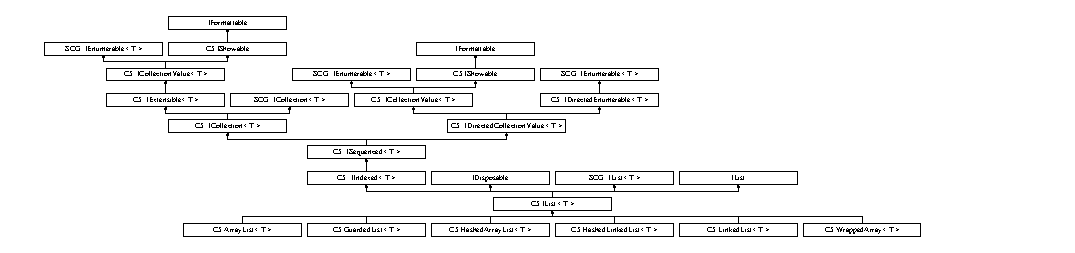
\includegraphics[height=2.957747cm]{interface_c5_1_1_i_list}
\end{center}
\end{figure}
\subsection*{Public Member Functions}
\begin{DoxyCompactItemize}
\item 
new bool \hyperlink{interface_c5_1_1_i_list_a800000d7344d000c1b8c67acda464a3d}{Add} (T item)
\item 
new void \hyperlink{interface_c5_1_1_i_list_aff6179e37b313d34596749484ae58ea4}{Clear} ()
\item 
new bool \hyperlink{interface_c5_1_1_i_list_a108b607b042959d063e1ca77e242406c}{Contains} (T item)
\item 
new void \hyperlink{interface_c5_1_1_i_list_a6fef986271bdc88a6f38cb15bd15690f}{Copy\+To} (T\mbox{[}$\,$\mbox{]} array, int index)
\item 
new bool \hyperlink{interface_c5_1_1_i_list_a14dd6b1e7f06807dc6a45edf0f83dfbd}{Remove} (T item)
\item 
new int \hyperlink{interface_c5_1_1_i_list_a52658ee618f1557622d766d7a348910a}{Index\+Of} (T item)
\begin{DoxyCompactList}\small\item\em Searches for an item in the list going forwards from the start. \end{DoxyCompactList}\item 
new T \hyperlink{interface_c5_1_1_i_list_a9fbcd9c55aae61134321939d0b104cc0}{Remove\+At} (int index)
\begin{DoxyCompactList}\small\item\em Remove the item at a specific position of the list. \end{DoxyCompactList}\item 
void \hyperlink{interface_c5_1_1_i_list_a80df9055583216f4498d3711c9658d1f}{Insert} (\hyperlink{interface_c5_1_1_i_list}{I\+List}$<$ T $>$ pointer, T item)
\begin{DoxyCompactList}\small\item\em Insert an item at the end of a compatible view, used as a pointer. \end{DoxyCompactList}\item 
void \hyperlink{interface_c5_1_1_i_list_a2dd0bf119dee26610ce56283da7d7d11}{Insert\+First} (T item)
\begin{DoxyCompactList}\small\item\em Insert an item at the front of this list. 
\begin{DoxyExceptions}{Exceptions}
{\em \hyperlink{class_c5_1_1_duplicate_not_allowed_exception}{Duplicate\+Not\+Allowed\+Exception}} & if the list has \\
\hline
\end{DoxyExceptions}
\end{DoxyCompactList}\item 
void \hyperlink{interface_c5_1_1_i_list_adbb76aa84c81cf3d93130ed3d3abd967}{Insert\+Last} (T item)
\begin{DoxyCompactList}\small\item\em Insert an item at the back of this list. 
\begin{DoxyExceptions}{Exceptions}
{\em \hyperlink{class_c5_1_1_duplicate_not_allowed_exception}{Duplicate\+Not\+Allowed\+Exception}} & if the list has \\
\hline
\end{DoxyExceptions}
\end{DoxyCompactList}\item 
void \hyperlink{interface_c5_1_1_i_list_a551f34466ccd64b90929d8a92b984dc5}{Insert\+All} (int index, S\+C\+G.\+I\+Enumerable$<$ T $>$ items)
\begin{DoxyCompactList}\small\item\em Insert into this list all items from an enumerable collection starting at a particular index. \end{DoxyCompactList}\item 
\hyperlink{interface_c5_1_1_i_list}{I\+List}$<$ T $>$ \hyperlink{interface_c5_1_1_i_list_a8bd6c307e2b3e5cbd50e92dde854a1d0}{Find\+All} (Func$<$ T, bool $>$ filter)
\begin{DoxyCompactList}\small\item\em Create a new list consisting of the items of this list satisfying a certain predicate. \end{DoxyCompactList}\item 
\hyperlink{interface_c5_1_1_i_list}{I\+List}$<$ V $>$ \hyperlink{interface_c5_1_1_i_list_a8cf8a4682fe990ce32d7cf4a2bec84b6}{Map$<$ V $>$} (Func$<$ T, V $>$ mapper)
\begin{DoxyCompactList}\small\item\em Create a new list consisting of the results of mapping all items of this list. The new list will use the default equality\+Comparer for the item type V. \end{DoxyCompactList}\item 
\hyperlink{interface_c5_1_1_i_list}{I\+List}$<$ V $>$ \hyperlink{interface_c5_1_1_i_list_ad84aa90d1111a8cb7ea1226d8cfadab9}{Map$<$ V $>$} (Func$<$ T, V $>$ mapper, S\+C\+G.\+I\+Equality\+Comparer$<$ V $>$ equality\+Comparer)
\begin{DoxyCompactList}\small\item\em Create a new list consisting of the results of mapping all items of this list. The new list will use a specified equality\+Comparer for the item type. \end{DoxyCompactList}\item 
T \hyperlink{interface_c5_1_1_i_list_ae0d9be125f478fed048c4c08159ae399}{Remove} ()
\begin{DoxyCompactList}\small\item\em Remove one item from the list\+: from the front if \end{DoxyCompactList}\item 
T \hyperlink{interface_c5_1_1_i_list_a6f5c3f67673d43604aa28a7d2b6508ff}{Remove\+First} ()
\begin{DoxyCompactList}\small\item\em Remove one item from the front of the list. 
\begin{DoxyExceptions}{Exceptions}
{\em \hyperlink{class_c5_1_1_no_such_item_exception}{No\+Such\+Item\+Exception}} & if this list is empty. \\
\hline
\end{DoxyExceptions}
\end{DoxyCompactList}\item 
T \hyperlink{interface_c5_1_1_i_list_adfbae9e7ea5cb9ff3e0fd45f1201334a}{Remove\+Last} ()
\begin{DoxyCompactList}\small\item\em Remove one item from the back of the list. 
\begin{DoxyExceptions}{Exceptions}
{\em \hyperlink{class_c5_1_1_no_such_item_exception}{No\+Such\+Item\+Exception}} & if this list is empty. \\
\hline
\end{DoxyExceptions}
\end{DoxyCompactList}\item 
\hyperlink{interface_c5_1_1_i_list}{I\+List}$<$ T $>$ \hyperlink{interface_c5_1_1_i_list_a402c21a9b1f0e2295303d35b6db5d273}{View} (int start, int count)
\begin{DoxyCompactList}\small\item\em Create a list view on this list. 
\begin{DoxyExceptions}{Exceptions}
{\em Argument\+Out\+Of\+Range\+Exception} & if the view would not fit into this list. \\
\hline
\end{DoxyExceptions}
\end{DoxyCompactList}\item 
\hyperlink{interface_c5_1_1_i_list}{I\+List}$<$ T $>$ \hyperlink{interface_c5_1_1_i_list_aefcdef9983913d18ae05394e77a44c71}{View\+Of} (T item)
\begin{DoxyCompactList}\small\item\em Create a list view on this list containing the (first) occurrence of a particular item. 
\begin{DoxyExceptions}{Exceptions}
{\em \hyperlink{class_c5_1_1_no_such_item_exception}{No\+Such\+Item\+Exception}} & if the item is not in this list. \\
\hline
\end{DoxyExceptions}
\end{DoxyCompactList}\item 
\hyperlink{interface_c5_1_1_i_list}{I\+List}$<$ T $>$ \hyperlink{interface_c5_1_1_i_list_a251c36fe72c9bc661d449bfd0ea90528}{Last\+View\+Of} (T item)
\begin{DoxyCompactList}\small\item\em Create a list view on this list containing the last occurrence of a particular item. 
\begin{DoxyExceptions}{Exceptions}
{\em \hyperlink{class_c5_1_1_no_such_item_exception}{No\+Such\+Item\+Exception}} & if the item is not in this list. \\
\hline
\end{DoxyExceptions}
\end{DoxyCompactList}\item 
\hyperlink{interface_c5_1_1_i_list}{I\+List}$<$ T $>$ \hyperlink{interface_c5_1_1_i_list_a5ef3eff3f13a9a69071dacefbf43f80b}{Slide} (int offset)
\begin{DoxyCompactList}\small\item\em Slide this list view along the underlying list. \end{DoxyCompactList}\item 
\hyperlink{interface_c5_1_1_i_list}{I\+List}$<$ T $>$ \hyperlink{interface_c5_1_1_i_list_a20b4e11e6d69d4251af92b666aa16004}{Slide} (int offset, int size)
\begin{DoxyCompactList}\small\item\em Slide this list view along the underlying list, changing its size. \end{DoxyCompactList}\item 
bool \hyperlink{interface_c5_1_1_i_list_a727578a3060d08dba6a065c5d90b77bd}{Try\+Slide} (int offset)
\item 
bool \hyperlink{interface_c5_1_1_i_list_a04c6671051fdef61f2b199c66bbfaa21}{Try\+Slide} (int offset, int size)
\item 
\hyperlink{interface_c5_1_1_i_list}{I\+List}$<$ T $>$ \hyperlink{interface_c5_1_1_i_list_a1fb50b61d1fb0117bf1ebcd4bf06dbfa}{Span} (\hyperlink{interface_c5_1_1_i_list}{I\+List}$<$ T $>$ other\+View)
\item 
void \hyperlink{interface_c5_1_1_i_list_aea3fef718431d1ab504e15457e7fda1c}{Reverse} ()
\begin{DoxyCompactList}\small\item\em Reverse the list so the items are in the opposite sequence order. \end{DoxyCompactList}\item 
bool \hyperlink{interface_c5_1_1_i_list_aadf94b51e2c383ebda5a9f48820ef9bb}{Is\+Sorted} ()
\begin{DoxyCompactList}\small\item\em Check if this list is sorted according to the default sorting order for the item type T, as defined by the T\+:\+C5.\+Comparer`1 class \end{DoxyCompactList}\item 
bool \hyperlink{interface_c5_1_1_i_list_ad7a87f535eab2f950eb4ad3311f3385f}{Is\+Sorted} (S\+C\+G.\+I\+Comparer$<$ T $>$ comparer)
\begin{DoxyCompactList}\small\item\em Check if this list is sorted according to a specific sorting order. \end{DoxyCompactList}\item 
void \hyperlink{interface_c5_1_1_i_list_ad65ec59c8caf18dbf8cf795edf45bce5}{Sort} ()
\begin{DoxyCompactList}\small\item\em Sort the items of the list according to the default sorting order for the item type T, as defined by the T\+:\+C5.\+Comparer`1 class \end{DoxyCompactList}\item 
void \hyperlink{interface_c5_1_1_i_list_ad6708e13ea86ba9317c5f03505bba7fb}{Sort} (S\+C\+G.\+I\+Comparer$<$ T $>$ comparer)
\begin{DoxyCompactList}\small\item\em Sort the items of the list according to a specified sorting order. \end{DoxyCompactList}\item 
void \hyperlink{interface_c5_1_1_i_list_abec18a307f13a6f7e9ef9bd1f131c9e2}{Shuffle} ()
\begin{DoxyCompactList}\small\item\em Randomly shuffle the items of this list. \end{DoxyCompactList}\item 
void \hyperlink{interface_c5_1_1_i_list_afc33a89830008ad176dfd0c67ceb8b12}{Shuffle} (Random rnd)
\begin{DoxyCompactList}\small\item\em Shuffle the items of this list according to a specific random source. \end{DoxyCompactList}\end{DoxyCompactItemize}
\subsection*{Properties}
\begin{DoxyCompactItemize}
\item 
T \hyperlink{interface_c5_1_1_i_list_a4bf9eeadd149cdffd72702f4ab1db0ba}{First}\hspace{0.3cm}{\ttfamily  \mbox{[}get\mbox{]}}
\item 
T \hyperlink{interface_c5_1_1_i_list_a7544fb96e486622500dc684352eac27b}{Last}\hspace{0.3cm}{\ttfamily  \mbox{[}get\mbox{]}}
\item 
bool \hyperlink{interface_c5_1_1_i_list_a0c804cfc13feed69e308ca37a32c872d}{F\+I\+F\+O}\hspace{0.3cm}{\ttfamily  \mbox{[}get, set\mbox{]}}
\begin{DoxyCompactList}\small\item\em Since \end{DoxyCompactList}\item 
bool \hyperlink{interface_c5_1_1_i_list_a265a2e21d24096940bc8c51ff7255a9b}{Is\+Fixed\+Size}\hspace{0.3cm}{\ttfamily  \mbox{[}get\mbox{]}}
\item 
new T \hyperlink{interface_c5_1_1_i_list_a93fa9e99864a05d47bcc6a5e4bf7feb9}{this\mbox{[}int index\mbox{]}}\hspace{0.3cm}{\ttfamily  \mbox{[}get, set\mbox{]}}
\begin{DoxyCompactList}\small\item\em On this list, this indexer is read/write. \end{DoxyCompactList}\item 
new int \hyperlink{interface_c5_1_1_i_list_a91519e08da04aef3233a65779f1b9942}{Count}\hspace{0.3cm}{\ttfamily  \mbox{[}get\mbox{]}}
\item 
new bool \hyperlink{interface_c5_1_1_i_list_a413032c05b1f8f4f060afb4ab3f3b579}{Is\+Read\+Only}\hspace{0.3cm}{\ttfamily  \mbox{[}get\mbox{]}}
\item 
\hyperlink{interface_c5_1_1_i_list}{I\+List}$<$ T $>$ \hyperlink{interface_c5_1_1_i_list_a2cdfa7ff17c18708340c56ae79f290bb}{Underlying}\hspace{0.3cm}{\ttfamily  \mbox{[}get\mbox{]}}
\begin{DoxyCompactList}\small\item\em Null if this list is not a view. \end{DoxyCompactList}\item 
int \hyperlink{interface_c5_1_1_i_list_a018e889717be028a6190964c98e10c63}{Offset}\hspace{0.3cm}{\ttfamily  \mbox{[}get\mbox{]}}
\item 
bool \hyperlink{interface_c5_1_1_i_list_ade26b03c600c09845c51fa9c36b24f15}{Is\+Valid}\hspace{0.3cm}{\ttfamily  \mbox{[}get\mbox{]}}
\end{DoxyCompactItemize}
\subsection*{Additional Inherited Members}


\subsection{Detailed Description}
This is an indexed collection, where the item order is chosen by the user at insertion time. 

N\+B\+N\+B\+N\+B\+: we need a description of the view functionality here! 

\subsection{Member Function Documentation}
\hypertarget{interface_c5_1_1_i_list_a800000d7344d000c1b8c67acda464a3d}{}\index{C5\+::\+I\+List@{C5\+::\+I\+List}!Add@{Add}}
\index{Add@{Add}!C5\+::\+I\+List@{C5\+::\+I\+List}}
\subsubsection[{Add(\+T item)}]{\setlength{\rightskip}{0pt plus 5cm}new bool {\bf C5.\+I\+List}$<$ T $>$.Add (
\begin{DoxyParamCaption}
\item[{T}]{item}
\end{DoxyParamCaption}
)}\label{interface_c5_1_1_i_list_a800000d7344d000c1b8c67acda464a3d}





\begin{DoxyParams}{Parameters}
{\em item} & \\
\hline
\end{DoxyParams}
\begin{DoxyReturn}{Returns}

\end{DoxyReturn}


Implements \hyperlink{interface_c5_1_1_i_collection_a525115f252ddca586fcbf1a0127be614}{C5.\+I\+Collection$<$ T $>$}.



Implemented in \hyperlink{class_c5_1_1_hashed_linked_list_afcfc7b8da2f00ad7d8e3decadadd74bc}{C5.\+Hashed\+Linked\+List$<$ T $>$}, \hyperlink{class_c5_1_1_linked_list_ac205fdb2cfc336ee2c2843c04fcbad41}{C5.\+Linked\+List$<$ T $>$}, \hyperlink{class_c5_1_1_hashed_array_list_a4606087ab02e09f75ce6810b7a9d11a4}{C5.\+Hashed\+Array\+List$<$ T $>$}, \hyperlink{class_c5_1_1_array_list_a31f07a779aa64ee15f6875ab74682cb5}{C5.\+Array\+List$<$ T $>$}, and \hyperlink{class_c5_1_1_wrapped_array_a5be2e0d6422cbc8597e1bc7571b41048}{C5.\+Wrapped\+Array$<$ T $>$}.

\hypertarget{interface_c5_1_1_i_list_aff6179e37b313d34596749484ae58ea4}{}\index{C5\+::\+I\+List@{C5\+::\+I\+List}!Clear@{Clear}}
\index{Clear@{Clear}!C5\+::\+I\+List@{C5\+::\+I\+List}}
\subsubsection[{Clear()}]{\setlength{\rightskip}{0pt plus 5cm}new void {\bf C5.\+I\+List}$<$ T $>$.Clear (
\begin{DoxyParamCaption}
{}
\end{DoxyParamCaption}
)}\label{interface_c5_1_1_i_list_aff6179e37b313d34596749484ae58ea4}






Implements \hyperlink{interface_c5_1_1_i_collection_abd83166ac00b3d36225d988fd4603e97}{C5.\+I\+Collection$<$ T $>$}.



Implemented in \hyperlink{class_c5_1_1_hashed_linked_list_a3d890e2da8746df9cf82d3ccaf561d44}{C5.\+Hashed\+Linked\+List$<$ T $>$}, \hyperlink{class_c5_1_1_linked_list_a936ee524a650660d23b62ff74ae306d9}{C5.\+Linked\+List$<$ T $>$}, \hyperlink{class_c5_1_1_hashed_array_list_aeca323e5f962607ee4384549aaba5d28}{C5.\+Hashed\+Array\+List$<$ T $>$}, \hyperlink{class_c5_1_1_array_list_a1ed4a8838cc6a215101b6af156e7da08}{C5.\+Array\+List$<$ T $>$}, and \hyperlink{class_c5_1_1_wrapped_array_aa57bfc8881b390314629e9830759eee5}{C5.\+Wrapped\+Array$<$ T $>$}.

\hypertarget{interface_c5_1_1_i_list_a108b607b042959d063e1ca77e242406c}{}\index{C5\+::\+I\+List@{C5\+::\+I\+List}!Contains@{Contains}}
\index{Contains@{Contains}!C5\+::\+I\+List@{C5\+::\+I\+List}}
\subsubsection[{Contains(\+T item)}]{\setlength{\rightskip}{0pt plus 5cm}new bool {\bf C5.\+I\+List}$<$ T $>$.Contains (
\begin{DoxyParamCaption}
\item[{T}]{item}
\end{DoxyParamCaption}
)}\label{interface_c5_1_1_i_list_a108b607b042959d063e1ca77e242406c}





\begin{DoxyParams}{Parameters}
{\em item} & \\
\hline
\end{DoxyParams}
\begin{DoxyReturn}{Returns}

\end{DoxyReturn}


Implements \hyperlink{interface_c5_1_1_i_collection_a4de01b6d77ea5eaffccc8267b4454cdd}{C5.\+I\+Collection$<$ T $>$}.



Implemented in \hyperlink{class_c5_1_1_hashed_linked_list_a210cb416cd7418c59c89b99e2fce7bf8}{C5.\+Hashed\+Linked\+List$<$ T $>$}, \hyperlink{class_c5_1_1_linked_list_a9d3273641ee62248a93ed0eb58bed66a}{C5.\+Linked\+List$<$ T $>$}, \hyperlink{class_c5_1_1_hashed_array_list_a4b108299a930ceaecd8484023a656cf4}{C5.\+Hashed\+Array\+List$<$ T $>$}, \hyperlink{class_c5_1_1_array_list_a481c1d9104e4c5fbd4dd79be7a1e5c38}{C5.\+Array\+List$<$ T $>$}, and \hyperlink{class_c5_1_1_wrapped_array_aeff3477a858a6f79b120be3ca1fd7c40}{C5.\+Wrapped\+Array$<$ T $>$}.

\hypertarget{interface_c5_1_1_i_list_a6fef986271bdc88a6f38cb15bd15690f}{}\index{C5\+::\+I\+List@{C5\+::\+I\+List}!Copy\+To@{Copy\+To}}
\index{Copy\+To@{Copy\+To}!C5\+::\+I\+List@{C5\+::\+I\+List}}
\subsubsection[{Copy\+To(\+T[] array, int index)}]{\setlength{\rightskip}{0pt plus 5cm}new void {\bf C5.\+I\+List}$<$ T $>$.Copy\+To (
\begin{DoxyParamCaption}
\item[{T\mbox{[}$\,$\mbox{]}}]{array, }
\item[{int}]{index}
\end{DoxyParamCaption}
)}\label{interface_c5_1_1_i_list_a6fef986271bdc88a6f38cb15bd15690f}





\begin{DoxyParams}{Parameters}
{\em array} & \\
\hline
{\em index} & \\
\hline
\end{DoxyParams}


Implements \hyperlink{interface_c5_1_1_i_collection_aa2f928b7057eb84a1572307123e8239e}{C5.\+I\+Collection$<$ T $>$}.



Implemented in \hyperlink{class_c5_1_1_wrapped_array_a3dfd50eb13f5b3f90445e217214fae96}{C5.\+Wrapped\+Array$<$ T $>$}.

\hypertarget{interface_c5_1_1_i_list_a8bd6c307e2b3e5cbd50e92dde854a1d0}{}\index{C5\+::\+I\+List@{C5\+::\+I\+List}!Find\+All@{Find\+All}}
\index{Find\+All@{Find\+All}!C5\+::\+I\+List@{C5\+::\+I\+List}}
\subsubsection[{Find\+All(\+Func$<$ T, bool $>$ filter)}]{\setlength{\rightskip}{0pt plus 5cm}{\bf I\+List}$<$T$>$ {\bf C5.\+I\+List}$<$ T $>$.Find\+All (
\begin{DoxyParamCaption}
\item[{Func$<$ T, bool $>$}]{filter}
\end{DoxyParamCaption}
)}\label{interface_c5_1_1_i_list_a8bd6c307e2b3e5cbd50e92dde854a1d0}


Create a new list consisting of the items of this list satisfying a certain predicate. 


\begin{DoxyParams}{Parameters}
{\em filter} & The filter delegate defining the predicate.\\
\hline
\end{DoxyParams}
\begin{DoxyReturn}{Returns}
The new list.
\end{DoxyReturn}


Implemented in \hyperlink{class_c5_1_1_hashed_linked_list_a4a12ba4a72a0d544589a4aabba1c63de}{C5.\+Hashed\+Linked\+List$<$ T $>$}, \hyperlink{class_c5_1_1_linked_list_a40efdf9ab3f9c34b6cdb1a408d2c97ac}{C5.\+Linked\+List$<$ T $>$}, \hyperlink{class_c5_1_1_guarded_list_a33bf64be5a6c3affeaba0e652c338811}{C5.\+Guarded\+List$<$ T $>$}, \hyperlink{class_c5_1_1_hashed_array_list_a44d89e2d1a233ee63a3e4efdee389585}{C5.\+Hashed\+Array\+List$<$ T $>$}, \hyperlink{class_c5_1_1_array_list_a8d970094faac5c6940db43796264b751}{C5.\+Array\+List$<$ T $>$}, and \hyperlink{class_c5_1_1_wrapped_array_a6580cb9eae8a2c617ed0d5ccbb669464}{C5.\+Wrapped\+Array$<$ T $>$}.

\hypertarget{interface_c5_1_1_i_list_a52658ee618f1557622d766d7a348910a}{}\index{C5\+::\+I\+List@{C5\+::\+I\+List}!Index\+Of@{Index\+Of}}
\index{Index\+Of@{Index\+Of}!C5\+::\+I\+List@{C5\+::\+I\+List}}
\subsubsection[{Index\+Of(\+T item)}]{\setlength{\rightskip}{0pt plus 5cm}new int {\bf C5.\+I\+List}$<$ T $>$.Index\+Of (
\begin{DoxyParamCaption}
\item[{T}]{item}
\end{DoxyParamCaption}
)}\label{interface_c5_1_1_i_list_a52658ee618f1557622d766d7a348910a}


Searches for an item in the list going forwards from the start. 


\begin{DoxyParams}{Parameters}
{\em item} & Item to search for.\\
\hline
\end{DoxyParams}
\begin{DoxyReturn}{Returns}
Index of item from start. A negative number if item not found, namely the one\textquotesingle{}s complement of the index at which the Add operation would put the item.
\end{DoxyReturn}


Implements \hyperlink{interface_c5_1_1_i_indexed_abad58598415e0383ddbc9275db69d92a}{C5.\+I\+Indexed$<$ T $>$}.



Implemented in \hyperlink{class_c5_1_1_hashed_linked_list_aca8634364d0bfec4b0d2bb8b7c6f5c98}{C5.\+Hashed\+Linked\+List$<$ T $>$}, \hyperlink{class_c5_1_1_guarded_list_aac2b7de89c7556b8a1c0b49dad25174f}{C5.\+Guarded\+List$<$ T $>$}, \hyperlink{class_c5_1_1_linked_list_a4dc305430081a02d96b65c285a61be7b}{C5.\+Linked\+List$<$ T $>$}, \hyperlink{class_c5_1_1_hashed_array_list_a6d13105e7f303fc04310801abed22946}{C5.\+Hashed\+Array\+List$<$ T $>$}, \hyperlink{class_c5_1_1_array_list_ae94dff251b125331c450b396418bb1be}{C5.\+Array\+List$<$ T $>$}, and \hyperlink{class_c5_1_1_wrapped_array_a459af83c432f3dbc167d406c4632fb0e}{C5.\+Wrapped\+Array$<$ T $>$}.

\hypertarget{interface_c5_1_1_i_list_a80df9055583216f4498d3711c9658d1f}{}\index{C5\+::\+I\+List@{C5\+::\+I\+List}!Insert@{Insert}}
\index{Insert@{Insert}!C5\+::\+I\+List@{C5\+::\+I\+List}}
\subsubsection[{Insert(\+I\+List$<$ T $>$ pointer, T item)}]{\setlength{\rightskip}{0pt plus 5cm}void {\bf C5.\+I\+List}$<$ T $>$.Insert (
\begin{DoxyParamCaption}
\item[{{\bf I\+List}$<$ T $>$}]{pointer, }
\item[{T}]{item}
\end{DoxyParamCaption}
)}\label{interface_c5_1_1_i_list_a80df9055583216f4498d3711c9658d1f}


Insert an item at the end of a compatible view, used as a pointer. 

The {\ttfamily pointer} must be a view on the same list as {\ttfamily this} and the endpoitn of {\ttfamily pointer} must be a valid insertion point of {\ttfamily this}


\begin{DoxyExceptions}{Exceptions}
{\em \hyperlink{class_c5_1_1_incompatible_view_exception}{Incompatible\+View\+Exception}} & If 
\begin{DoxyCode}
pointer
\end{DoxyCode}
 is not a view on the same list as 
\begin{DoxyCode}
\textcolor{keyword}{this}
\end{DoxyCode}
\\
\hline
{\em Index\+Out\+Of\+Range\+Exception} & {\bfseries ??????} if the endpoint of 
\begin{DoxyCode}
pointer
\end{DoxyCode}
 is not inside 
\begin{DoxyCode}
\textcolor{keyword}{this}
\end{DoxyCode}
\\
\hline
{\em \hyperlink{class_c5_1_1_duplicate_not_allowed_exception}{Duplicate\+Not\+Allowed\+Exception}} & if the list has 
\begin{DoxyCode}
\hyperlink{interface_c5_1_1_i_extensible_a1f2129ec206bc1a66e4a62874a67dff7}{AllowsDuplicates}==\textcolor{keyword}{false}
\end{DoxyCode}
 and the item is already in the list.\\
\hline
\end{DoxyExceptions}

\begin{DoxyParams}{Parameters}
{\em pointer} & \\
\hline
{\em item} & \\
\hline
\end{DoxyParams}


Implemented in \hyperlink{class_c5_1_1_guarded_list_ae15de88d818447d3b25217d1b1298f27}{C5.\+Guarded\+List$<$ T $>$}, \hyperlink{class_c5_1_1_hashed_linked_list_a3ad04f5ddf6a1a8dd8ca517f7298aee0}{C5.\+Hashed\+Linked\+List$<$ T $>$}, \hyperlink{class_c5_1_1_linked_list_a4b4a52f0c0f07eca6ccaa1ed627af6df}{C5.\+Linked\+List$<$ T $>$}, \hyperlink{class_c5_1_1_hashed_array_list_af2232ffdbc3b0970aeebcbda288f22c1}{C5.\+Hashed\+Array\+List$<$ T $>$}, \hyperlink{class_c5_1_1_array_list_a9622480e8a1e187bb4174cd1d149b1f9}{C5.\+Array\+List$<$ T $>$}, and \hyperlink{class_c5_1_1_wrapped_array_a25630c81bea9df1f81d947bc4315b1e4}{C5.\+Wrapped\+Array$<$ T $>$}.

\hypertarget{interface_c5_1_1_i_list_a551f34466ccd64b90929d8a92b984dc5}{}\index{C5\+::\+I\+List@{C5\+::\+I\+List}!Insert\+All@{Insert\+All}}
\index{Insert\+All@{Insert\+All}!C5\+::\+I\+List@{C5\+::\+I\+List}}
\subsubsection[{Insert\+All(int index, S\+C\+G.\+I\+Enumerable$<$ T $>$ items)}]{\setlength{\rightskip}{0pt plus 5cm}void {\bf C5.\+I\+List}$<$ T $>$.Insert\+All (
\begin{DoxyParamCaption}
\item[{int}]{index, }
\item[{S\+C\+G.\+I\+Enumerable$<$ T $>$}]{items}
\end{DoxyParamCaption}
)}\label{interface_c5_1_1_i_list_a551f34466ccd64b90929d8a92b984dc5}


Insert into this list all items from an enumerable collection starting at a particular index. 


\begin{DoxyExceptions}{Exceptions}
{\em Index\+Out\+Of\+Range\+Exception} & if 
\begin{DoxyCode}
index
\end{DoxyCode}
 is negative or $>$ the size of the collection.\\
\hline
{\em \hyperlink{class_c5_1_1_duplicate_not_allowed_exception}{Duplicate\+Not\+Allowed\+Exception}} & if the list has 
\begin{DoxyCode}
\hyperlink{interface_c5_1_1_i_extensible_a1f2129ec206bc1a66e4a62874a67dff7}{AllowsDuplicates}==\textcolor{keyword}{false}
\end{DoxyCode}
 and one of the items to insert is already in the list.\\
\hline
\end{DoxyExceptions}

\begin{DoxyParams}{Parameters}
{\em index} & Index to start inserting at\\
\hline
{\em items} & Items to insert\\
\hline
\end{DoxyParams}


Implemented in \hyperlink{class_c5_1_1_guarded_list_ac87627af2f8b971c1c079e63e64b9953}{C5.\+Guarded\+List$<$ T $>$}, \hyperlink{class_c5_1_1_hashed_linked_list_a6e309a1f1e92f363e9a49695cb3e5ce2}{C5.\+Hashed\+Linked\+List$<$ T $>$}, \hyperlink{class_c5_1_1_linked_list_adfc95cf986e2a54a5376e238868adf9c}{C5.\+Linked\+List$<$ T $>$}, \hyperlink{class_c5_1_1_hashed_array_list_a79d133efc3cafb5a74b265b0c85529f8}{C5.\+Hashed\+Array\+List$<$ T $>$}, \hyperlink{class_c5_1_1_array_list_a587910564b15fa1c71b6ba72ff7a4395}{C5.\+Array\+List$<$ T $>$}, and \hyperlink{class_c5_1_1_wrapped_array_a8dfe7a28dc0f1b1a3b3548d3cfdd3959}{C5.\+Wrapped\+Array$<$ T $>$}.

\hypertarget{interface_c5_1_1_i_list_a2dd0bf119dee26610ce56283da7d7d11}{}\index{C5\+::\+I\+List@{C5\+::\+I\+List}!Insert\+First@{Insert\+First}}
\index{Insert\+First@{Insert\+First}!C5\+::\+I\+List@{C5\+::\+I\+List}}
\subsubsection[{Insert\+First(\+T item)}]{\setlength{\rightskip}{0pt plus 5cm}void {\bf C5.\+I\+List}$<$ T $>$.Insert\+First (
\begin{DoxyParamCaption}
\item[{T}]{item}
\end{DoxyParamCaption}
)}\label{interface_c5_1_1_i_list_a2dd0bf119dee26610ce56283da7d7d11}


Insert an item at the front of this list. 
\begin{DoxyExceptions}{Exceptions}
{\em \hyperlink{class_c5_1_1_duplicate_not_allowed_exception}{Duplicate\+Not\+Allowed\+Exception}} & if the list has \\
\hline
\end{DoxyExceptions}


{\ttfamily Allows\+Duplicates==false} and the item is already in the list. 


\begin{DoxyParams}{Parameters}
{\em item} & The item to insert.\\
\hline
\end{DoxyParams}


Implemented in \hyperlink{class_c5_1_1_guarded_list_a5f5b548fa5704e9a9d83532280a3a0b0}{C5.\+Guarded\+List$<$ T $>$}, \hyperlink{class_c5_1_1_hashed_linked_list_ae02598bb941fbd2665b3b05c317aeadb}{C5.\+Hashed\+Linked\+List$<$ T $>$}, \hyperlink{class_c5_1_1_linked_list_a6067d9bec9351fc0005cfe9871bd2eb0}{C5.\+Linked\+List$<$ T $>$}, \hyperlink{class_c5_1_1_hashed_array_list_a0466cbd0ea303e0ba40e8611dfa3f721}{C5.\+Hashed\+Array\+List$<$ T $>$}, \hyperlink{class_c5_1_1_array_list_a272dc95d5ca8c2ce1b3ab43e3c56a4ce}{C5.\+Array\+List$<$ T $>$}, and \hyperlink{class_c5_1_1_wrapped_array_a788dd6164116d45b8043fd515a707e6d}{C5.\+Wrapped\+Array$<$ T $>$}.

\hypertarget{interface_c5_1_1_i_list_adbb76aa84c81cf3d93130ed3d3abd967}{}\index{C5\+::\+I\+List@{C5\+::\+I\+List}!Insert\+Last@{Insert\+Last}}
\index{Insert\+Last@{Insert\+Last}!C5\+::\+I\+List@{C5\+::\+I\+List}}
\subsubsection[{Insert\+Last(\+T item)}]{\setlength{\rightskip}{0pt plus 5cm}void {\bf C5.\+I\+List}$<$ T $>$.Insert\+Last (
\begin{DoxyParamCaption}
\item[{T}]{item}
\end{DoxyParamCaption}
)}\label{interface_c5_1_1_i_list_adbb76aa84c81cf3d93130ed3d3abd967}


Insert an item at the back of this list. 
\begin{DoxyExceptions}{Exceptions}
{\em \hyperlink{class_c5_1_1_duplicate_not_allowed_exception}{Duplicate\+Not\+Allowed\+Exception}} & if the list has \\
\hline
\end{DoxyExceptions}


{\ttfamily Allows\+Duplicates==false} and the item is already in the list. 


\begin{DoxyParams}{Parameters}
{\em item} & The item to insert.\\
\hline
\end{DoxyParams}


Implemented in \hyperlink{class_c5_1_1_guarded_list_a0e0d36df19f7bdedf7c9929953381ab5}{C5.\+Guarded\+List$<$ T $>$}, \hyperlink{class_c5_1_1_hashed_linked_list_a315e3df7f01e031e71d2da0581ee2598}{C5.\+Hashed\+Linked\+List$<$ T $>$}, \hyperlink{class_c5_1_1_linked_list_a7499dfb54c0666ddd74f8f0bb53e30f7}{C5.\+Linked\+List$<$ T $>$}, \hyperlink{class_c5_1_1_hashed_array_list_a616672c94355ca1f07af3a2b2ffe51bb}{C5.\+Hashed\+Array\+List$<$ T $>$}, \hyperlink{class_c5_1_1_array_list_a31ce1aee48da6e5e90791c61af922a3b}{C5.\+Array\+List$<$ T $>$}, and \hyperlink{class_c5_1_1_wrapped_array_abe9ea4b00b84b312e033eabfb35d5d77}{C5.\+Wrapped\+Array$<$ T $>$}.

\hypertarget{interface_c5_1_1_i_list_aadf94b51e2c383ebda5a9f48820ef9bb}{}\index{C5\+::\+I\+List@{C5\+::\+I\+List}!Is\+Sorted@{Is\+Sorted}}
\index{Is\+Sorted@{Is\+Sorted}!C5\+::\+I\+List@{C5\+::\+I\+List}}
\subsubsection[{Is\+Sorted()}]{\setlength{\rightskip}{0pt plus 5cm}bool {\bf C5.\+I\+List}$<$ T $>$.Is\+Sorted (
\begin{DoxyParamCaption}
{}
\end{DoxyParamCaption}
)}\label{interface_c5_1_1_i_list_aadf94b51e2c383ebda5a9f48820ef9bb}


Check if this list is sorted according to the default sorting order for the item type T, as defined by the T\+:\+C5.\+Comparer`1 class 


\begin{DoxyExceptions}{Exceptions}
{\em \hyperlink{class_c5_1_1_not_comparable_exception}{Not\+Comparable\+Exception}} & if T is not comparable\\
\hline
\end{DoxyExceptions}
\begin{DoxyReturn}{Returns}
True if the list is sorted, else false.
\end{DoxyReturn}


Implemented in \hyperlink{class_c5_1_1_hashed_linked_list_ab34c0de0335ccd7d9d16efd159d4411b}{C5.\+Hashed\+Linked\+List$<$ T $>$}, \hyperlink{class_c5_1_1_guarded_list_a7f201d294ec23f1231ddf27350657537}{C5.\+Guarded\+List$<$ T $>$}, \hyperlink{class_c5_1_1_linked_list_abb78955cf98434f86b34ba8d363cb062}{C5.\+Linked\+List$<$ T $>$}, \hyperlink{class_c5_1_1_hashed_array_list_a7d8165aa133bc45c19481e7d74d2ceb7}{C5.\+Hashed\+Array\+List$<$ T $>$}, \hyperlink{class_c5_1_1_array_list_a9c15cf2f69d3459b4a22ecd854689768}{C5.\+Array\+List$<$ T $>$}, and \hyperlink{class_c5_1_1_wrapped_array_af134399df22e512094a27e95cd147b13}{C5.\+Wrapped\+Array$<$ T $>$}.

\hypertarget{interface_c5_1_1_i_list_ad7a87f535eab2f950eb4ad3311f3385f}{}\index{C5\+::\+I\+List@{C5\+::\+I\+List}!Is\+Sorted@{Is\+Sorted}}
\index{Is\+Sorted@{Is\+Sorted}!C5\+::\+I\+List@{C5\+::\+I\+List}}
\subsubsection[{Is\+Sorted(\+S\+C\+G.\+I\+Comparer$<$ T $>$ comparer)}]{\setlength{\rightskip}{0pt plus 5cm}bool {\bf C5.\+I\+List}$<$ T $>$.Is\+Sorted (
\begin{DoxyParamCaption}
\item[{S\+C\+G.\+I\+Comparer$<$ T $>$}]{comparer}
\end{DoxyParamCaption}
)}\label{interface_c5_1_1_i_list_ad7a87f535eab2f950eb4ad3311f3385f}


Check if this list is sorted according to a specific sorting order. 


\begin{DoxyParams}{Parameters}
{\em comparer} & The comparer defining the sorting order.\\
\hline
\end{DoxyParams}
\begin{DoxyReturn}{Returns}
True if the list is sorted, else false.
\end{DoxyReturn}


Implemented in \hyperlink{class_c5_1_1_hashed_linked_list_a7d539fd8712f39feca8e3b1c561e8850}{C5.\+Hashed\+Linked\+List$<$ T $>$}, \hyperlink{class_c5_1_1_guarded_list_a1a24999c136d34605f5d6b2f004e8610}{C5.\+Guarded\+List$<$ T $>$}, \hyperlink{class_c5_1_1_linked_list_a7cd3044aa3b164fbec60641619982507}{C5.\+Linked\+List$<$ T $>$}, \hyperlink{class_c5_1_1_hashed_array_list_a4ad671797c33a01e7faf008c184bfdc6}{C5.\+Hashed\+Array\+List$<$ T $>$}, \hyperlink{class_c5_1_1_array_list_a267b37f723053dcc17d03c789956332a}{C5.\+Array\+List$<$ T $>$}, and \hyperlink{class_c5_1_1_wrapped_array_a63b841f528e5b8b1768687b73e755644}{C5.\+Wrapped\+Array$<$ T $>$}.

\hypertarget{interface_c5_1_1_i_list_a251c36fe72c9bc661d449bfd0ea90528}{}\index{C5\+::\+I\+List@{C5\+::\+I\+List}!Last\+View\+Of@{Last\+View\+Of}}
\index{Last\+View\+Of@{Last\+View\+Of}!C5\+::\+I\+List@{C5\+::\+I\+List}}
\subsubsection[{Last\+View\+Of(\+T item)}]{\setlength{\rightskip}{0pt plus 5cm}{\bf I\+List}$<$T$>$ {\bf C5.\+I\+List}$<$ T $>$.Last\+View\+Of (
\begin{DoxyParamCaption}
\item[{T}]{item}
\end{DoxyParamCaption}
)}\label{interface_c5_1_1_i_list_a251c36fe72c9bc661d449bfd0ea90528}


Create a list view on this list containing the last occurrence of a particular item. 
\begin{DoxyExceptions}{Exceptions}
{\em \hyperlink{class_c5_1_1_no_such_item_exception}{No\+Such\+Item\+Exception}} & if the item is not in this list. \\
\hline
\end{DoxyExceptions}



\begin{DoxyParams}{Parameters}
{\em item} & The item to find.\\
\hline
\end{DoxyParams}
\begin{DoxyReturn}{Returns}
The new list view.
\end{DoxyReturn}


Implemented in \hyperlink{class_c5_1_1_hashed_linked_list_a3c61023f5a2ea2c6011b35dff34f4058}{C5.\+Hashed\+Linked\+List$<$ T $>$}, \hyperlink{class_c5_1_1_guarded_list_a48deee08c78c1e766fb4bbbbf88dc83a}{C5.\+Guarded\+List$<$ T $>$}, \hyperlink{class_c5_1_1_linked_list_ad1afcf3bee602e7899bebfeaf7b549ad}{C5.\+Linked\+List$<$ T $>$}, \hyperlink{class_c5_1_1_hashed_array_list_a137af82d41074860aff0ccfaa67fac60}{C5.\+Hashed\+Array\+List$<$ T $>$}, \hyperlink{class_c5_1_1_array_list_a501ef3474fc833061931a134daa2cab2}{C5.\+Array\+List$<$ T $>$}, and \hyperlink{class_c5_1_1_wrapped_array_a40efb134cd66039cafc0ebc09e3db6e5}{C5.\+Wrapped\+Array$<$ T $>$}.

\hypertarget{interface_c5_1_1_i_list_a8cf8a4682fe990ce32d7cf4a2bec84b6}{}\index{C5\+::\+I\+List@{C5\+::\+I\+List}!Map$<$ V $>$@{Map$<$ V $>$}}
\index{Map$<$ V $>$@{Map$<$ V $>$}!C5\+::\+I\+List@{C5\+::\+I\+List}}
\subsubsection[{Map$<$ V $>$(\+Func$<$ T, V $>$ mapper)}]{\setlength{\rightskip}{0pt plus 5cm}{\bf I\+List}$<$V$>$ {\bf C5.\+I\+List}$<$ T $>$.Map$<$ V $>$ (
\begin{DoxyParamCaption}
\item[{Func$<$ T, V $>$}]{mapper}
\end{DoxyParamCaption}
)}\label{interface_c5_1_1_i_list_a8cf8a4682fe990ce32d7cf4a2bec84b6}


Create a new list consisting of the results of mapping all items of this list. The new list will use the default equality\+Comparer for the item type V. 


\begin{DoxyTemplParams}{Template Parameters}
{\em V} & The type of items of the new list\\
\hline
\end{DoxyTemplParams}

\begin{DoxyParams}{Parameters}
{\em mapper} & The delegate defining the map.\\
\hline
\end{DoxyParams}
\begin{DoxyReturn}{Returns}
The new list.
\end{DoxyReturn}


Implemented in \hyperlink{class_c5_1_1_guarded_list_a383354c45a2b2edd71d58517a1e82920}{C5.\+Guarded\+List$<$ T $>$}, \hyperlink{class_c5_1_1_hashed_linked_list_adc35379b5a56bbaf7790dd26bcc8ab6b}{C5.\+Hashed\+Linked\+List$<$ T $>$}, \hyperlink{class_c5_1_1_linked_list_abbc04f5392972731a1df156e98c54c98}{C5.\+Linked\+List$<$ T $>$}, \hyperlink{class_c5_1_1_hashed_array_list_aacf59f051c56a96f62e5de97f1d51b87}{C5.\+Hashed\+Array\+List$<$ T $>$}, \hyperlink{class_c5_1_1_array_list_a7a973a5950c1f27d95cce3d8d3a5979f}{C5.\+Array\+List$<$ T $>$}, and \hyperlink{class_c5_1_1_wrapped_array_a319143ffc0237155b5633e4e5c61b474}{C5.\+Wrapped\+Array$<$ T $>$}.

\hypertarget{interface_c5_1_1_i_list_ad84aa90d1111a8cb7ea1226d8cfadab9}{}\index{C5\+::\+I\+List@{C5\+::\+I\+List}!Map$<$ V $>$@{Map$<$ V $>$}}
\index{Map$<$ V $>$@{Map$<$ V $>$}!C5\+::\+I\+List@{C5\+::\+I\+List}}
\subsubsection[{Map$<$ V $>$(\+Func$<$ T, V $>$ mapper, S\+C\+G.\+I\+Equality\+Comparer$<$ V $>$ equality\+Comparer)}]{\setlength{\rightskip}{0pt plus 5cm}{\bf I\+List}$<$V$>$ {\bf C5.\+I\+List}$<$ T $>$.Map$<$ V $>$ (
\begin{DoxyParamCaption}
\item[{Func$<$ T, V $>$}]{mapper, }
\item[{S\+C\+G.\+I\+Equality\+Comparer$<$ V $>$}]{equality\+Comparer}
\end{DoxyParamCaption}
)}\label{interface_c5_1_1_i_list_ad84aa90d1111a8cb7ea1226d8cfadab9}


Create a new list consisting of the results of mapping all items of this list. The new list will use a specified equality\+Comparer for the item type. 


\begin{DoxyTemplParams}{Template Parameters}
{\em V} & The type of items of the new list\\
\hline
\end{DoxyTemplParams}

\begin{DoxyParams}{Parameters}
{\em mapper} & The delegate defining the map.\\
\hline
{\em equality\+Comparer} & The equality\+Comparer to use for the new list\\
\hline
\end{DoxyParams}
\begin{DoxyReturn}{Returns}
The new list.
\end{DoxyReturn}


Implemented in \hyperlink{class_c5_1_1_guarded_list_a468610da48a606cd83a609bd116d277c}{C5.\+Guarded\+List$<$ T $>$}, \hyperlink{class_c5_1_1_hashed_linked_list_a5785aad402110c74b1d100ba504d1d90}{C5.\+Hashed\+Linked\+List$<$ T $>$}, \hyperlink{class_c5_1_1_linked_list_a72a7d7f8774986186f63c2dc2f8fceb7}{C5.\+Linked\+List$<$ T $>$}, \hyperlink{class_c5_1_1_hashed_array_list_a560e362c78363db5884315caaa4dd40a}{C5.\+Hashed\+Array\+List$<$ T $>$}, \hyperlink{class_c5_1_1_array_list_a3cc88a23901441ffca7b03f8445c6c6a}{C5.\+Array\+List$<$ T $>$}, and \hyperlink{class_c5_1_1_wrapped_array_a9297d4f2de04f4d3f72892992b702810}{C5.\+Wrapped\+Array$<$ T $>$}.

\hypertarget{interface_c5_1_1_i_list_a14dd6b1e7f06807dc6a45edf0f83dfbd}{}\index{C5\+::\+I\+List@{C5\+::\+I\+List}!Remove@{Remove}}
\index{Remove@{Remove}!C5\+::\+I\+List@{C5\+::\+I\+List}}
\subsubsection[{Remove(\+T item)}]{\setlength{\rightskip}{0pt plus 5cm}new bool {\bf C5.\+I\+List}$<$ T $>$.Remove (
\begin{DoxyParamCaption}
\item[{T}]{item}
\end{DoxyParamCaption}
)}\label{interface_c5_1_1_i_list_a14dd6b1e7f06807dc6a45edf0f83dfbd}





\begin{DoxyParams}{Parameters}
{\em item} & \\
\hline
\end{DoxyParams}
\begin{DoxyReturn}{Returns}

\end{DoxyReturn}


Implements \hyperlink{interface_c5_1_1_i_collection_ab4d6092ac09245ce46db91595fc1cdfe}{C5.\+I\+Collection$<$ T $>$}.



Implemented in \hyperlink{class_c5_1_1_hashed_linked_list_ad97f128fe00bf12c8e77678f08bd27e1}{C5.\+Hashed\+Linked\+List$<$ T $>$}, \hyperlink{class_c5_1_1_linked_list_a16561b02cc72e8d8191c32a84af13d81}{C5.\+Linked\+List$<$ T $>$}, \hyperlink{class_c5_1_1_hashed_array_list_a4453b3955bce1670914b4aa2f469b4c0}{C5.\+Hashed\+Array\+List$<$ T $>$}, \hyperlink{class_c5_1_1_array_list_a8e3d348ba6d557785028bee0b9a25bf8}{C5.\+Array\+List$<$ T $>$}, and \hyperlink{class_c5_1_1_wrapped_array_a3f312170b262e9f56b4d23442eb98029}{C5.\+Wrapped\+Array$<$ T $>$}.

\hypertarget{interface_c5_1_1_i_list_ae0d9be125f478fed048c4c08159ae399}{}\index{C5\+::\+I\+List@{C5\+::\+I\+List}!Remove@{Remove}}
\index{Remove@{Remove}!C5\+::\+I\+List@{C5\+::\+I\+List}}
\subsubsection[{Remove()}]{\setlength{\rightskip}{0pt plus 5cm}T {\bf C5.\+I\+List}$<$ T $>$.Remove (
\begin{DoxyParamCaption}
{}
\end{DoxyParamCaption}
)}\label{interface_c5_1_1_i_list_ae0d9be125f478fed048c4c08159ae399}


Remove one item from the list\+: from the front if 

{\ttfamily F\+I\+F\+O} is true, else from the back. 
\begin{DoxyExceptions}{Exceptions}
{\em \hyperlink{class_c5_1_1_no_such_item_exception}{No\+Such\+Item\+Exception}} & if this list is empty. 

\begin{DoxyReturn}{Returns}
The removed item.
\end{DoxyReturn}
\\
\hline
\end{DoxyExceptions}


Implemented in \hyperlink{class_c5_1_1_guarded_list_afdeda008aae91bbbe607012e0e64bac4}{C5.\+Guarded\+List$<$ T $>$}, \hyperlink{class_c5_1_1_hashed_linked_list_a899849bf8ad50e60206c8b3b59611eaf}{C5.\+Hashed\+Linked\+List$<$ T $>$}, \hyperlink{class_c5_1_1_linked_list_a91f46345f78948de9227a25acca79cf0}{C5.\+Linked\+List$<$ T $>$}, \hyperlink{class_c5_1_1_hashed_array_list_a36ab8321ad505bf9780d39a41d419f31}{C5.\+Hashed\+Array\+List$<$ T $>$}, \hyperlink{class_c5_1_1_array_list_a0bdb83e1cd5d4e6a75440f75c0fa7c9b}{C5.\+Array\+List$<$ T $>$}, and \hyperlink{class_c5_1_1_wrapped_array_a067a9891e0d7519b30a726a204d64237}{C5.\+Wrapped\+Array$<$ T $>$}.

\hypertarget{interface_c5_1_1_i_list_a9fbcd9c55aae61134321939d0b104cc0}{}\index{C5\+::\+I\+List@{C5\+::\+I\+List}!Remove\+At@{Remove\+At}}
\index{Remove\+At@{Remove\+At}!C5\+::\+I\+List@{C5\+::\+I\+List}}
\subsubsection[{Remove\+At(int index)}]{\setlength{\rightskip}{0pt plus 5cm}new T {\bf C5.\+I\+List}$<$ T $>$.Remove\+At (
\begin{DoxyParamCaption}
\item[{int}]{index}
\end{DoxyParamCaption}
)}\label{interface_c5_1_1_i_list_a9fbcd9c55aae61134321939d0b104cc0}


Remove the item at a specific position of the list. 


\begin{DoxyExceptions}{Exceptions}
{\em Index\+Out\+Of\+Range\+Exception} & if 
\begin{DoxyCode}
index
\end{DoxyCode}
 is negative or $>$= the size of the collection.\\
\hline
\end{DoxyExceptions}

\begin{DoxyParams}{Parameters}
{\em index} & The index of the item to remove.\\
\hline
\end{DoxyParams}
\begin{DoxyReturn}{Returns}
The removed item.
\end{DoxyReturn}


Implements \hyperlink{interface_c5_1_1_i_indexed_ac741e6d3d7c6a30bb8a013bb29591ca4}{C5.\+I\+Indexed$<$ T $>$}.



Implemented in \hyperlink{class_c5_1_1_hashed_linked_list_ae29691247778dcae44ae4a4482c4c94f}{C5.\+Hashed\+Linked\+List$<$ T $>$}, \hyperlink{class_c5_1_1_guarded_list_a051deb35bed74f188be08a40c1e79afa}{C5.\+Guarded\+List$<$ T $>$}, \hyperlink{class_c5_1_1_linked_list_ad5bcb57accd6b97265cf8c12efeda71c}{C5.\+Linked\+List$<$ T $>$}, \hyperlink{class_c5_1_1_hashed_array_list_a28dadd5b31e5daa8eb34728f0c31728a}{C5.\+Hashed\+Array\+List$<$ T $>$}, \hyperlink{class_c5_1_1_array_list_a0f3b4828a1c3ba06d035ad6f2aa491fc}{C5.\+Array\+List$<$ T $>$}, and \hyperlink{class_c5_1_1_wrapped_array_a01b30a7260874fcd043d01cabad29f55}{C5.\+Wrapped\+Array$<$ T $>$}.

\hypertarget{interface_c5_1_1_i_list_a6f5c3f67673d43604aa28a7d2b6508ff}{}\index{C5\+::\+I\+List@{C5\+::\+I\+List}!Remove\+First@{Remove\+First}}
\index{Remove\+First@{Remove\+First}!C5\+::\+I\+List@{C5\+::\+I\+List}}
\subsubsection[{Remove\+First()}]{\setlength{\rightskip}{0pt plus 5cm}T {\bf C5.\+I\+List}$<$ T $>$.Remove\+First (
\begin{DoxyParamCaption}
{}
\end{DoxyParamCaption}
)}\label{interface_c5_1_1_i_list_a6f5c3f67673d43604aa28a7d2b6508ff}


Remove one item from the front of the list. 
\begin{DoxyExceptions}{Exceptions}
{\em \hyperlink{class_c5_1_1_no_such_item_exception}{No\+Such\+Item\+Exception}} & if this list is empty. \\
\hline
\end{DoxyExceptions}


\begin{DoxyReturn}{Returns}
The removed item.
\end{DoxyReturn}


Implemented in \hyperlink{class_c5_1_1_guarded_list_a5cc22aac9bcdf45c68a285c21e8d1b8d}{C5.\+Guarded\+List$<$ T $>$}, \hyperlink{class_c5_1_1_hashed_linked_list_ab319b375d54035e9599a018ea4c6f342}{C5.\+Hashed\+Linked\+List$<$ T $>$}, \hyperlink{class_c5_1_1_linked_list_a4d86cb509302d7b05a2f2d12bc14c722}{C5.\+Linked\+List$<$ T $>$}, \hyperlink{class_c5_1_1_hashed_array_list_a569ec3b1a5fc7ab16bf6fc6eac5a2977}{C5.\+Hashed\+Array\+List$<$ T $>$}, \hyperlink{class_c5_1_1_array_list_aaf9d886025d96e91a9275055a37b984f}{C5.\+Array\+List$<$ T $>$}, and \hyperlink{class_c5_1_1_wrapped_array_a3b3917acf620f16ef736b75f25d4a8e3}{C5.\+Wrapped\+Array$<$ T $>$}.

\hypertarget{interface_c5_1_1_i_list_adfbae9e7ea5cb9ff3e0fd45f1201334a}{}\index{C5\+::\+I\+List@{C5\+::\+I\+List}!Remove\+Last@{Remove\+Last}}
\index{Remove\+Last@{Remove\+Last}!C5\+::\+I\+List@{C5\+::\+I\+List}}
\subsubsection[{Remove\+Last()}]{\setlength{\rightskip}{0pt plus 5cm}T {\bf C5.\+I\+List}$<$ T $>$.Remove\+Last (
\begin{DoxyParamCaption}
{}
\end{DoxyParamCaption}
)}\label{interface_c5_1_1_i_list_adfbae9e7ea5cb9ff3e0fd45f1201334a}


Remove one item from the back of the list. 
\begin{DoxyExceptions}{Exceptions}
{\em \hyperlink{class_c5_1_1_no_such_item_exception}{No\+Such\+Item\+Exception}} & if this list is empty. \\
\hline
\end{DoxyExceptions}


\begin{DoxyReturn}{Returns}
The removed item.
\end{DoxyReturn}


Implemented in \hyperlink{class_c5_1_1_guarded_list_abd9f4b23595221985b5b329b245c0abc}{C5.\+Guarded\+List$<$ T $>$}, \hyperlink{class_c5_1_1_hashed_linked_list_a0fc592e8e1c3667b8e65f3b32eafe863}{C5.\+Hashed\+Linked\+List$<$ T $>$}, \hyperlink{class_c5_1_1_linked_list_a66a4322035508335f3b8edff17d5f7c9}{C5.\+Linked\+List$<$ T $>$}, \hyperlink{class_c5_1_1_hashed_array_list_a3d58befa5b2087abe708a3c76ecdda88}{C5.\+Hashed\+Array\+List$<$ T $>$}, \hyperlink{class_c5_1_1_array_list_af26267e25450db0612a4eeb8210560c5}{C5.\+Array\+List$<$ T $>$}, and \hyperlink{class_c5_1_1_wrapped_array_a04f236941c2f7aef12997e6d305a1dcf}{C5.\+Wrapped\+Array$<$ T $>$}.

\hypertarget{interface_c5_1_1_i_list_aea3fef718431d1ab504e15457e7fda1c}{}\index{C5\+::\+I\+List@{C5\+::\+I\+List}!Reverse@{Reverse}}
\index{Reverse@{Reverse}!C5\+::\+I\+List@{C5\+::\+I\+List}}
\subsubsection[{Reverse()}]{\setlength{\rightskip}{0pt plus 5cm}void {\bf C5.\+I\+List}$<$ T $>$.Reverse (
\begin{DoxyParamCaption}
{}
\end{DoxyParamCaption}
)}\label{interface_c5_1_1_i_list_aea3fef718431d1ab504e15457e7fda1c}


Reverse the list so the items are in the opposite sequence order. 



Implemented in \hyperlink{class_c5_1_1_hashed_linked_list_a1390f0566000923c714fe19d1d2792d3}{C5.\+Hashed\+Linked\+List$<$ T $>$}, \hyperlink{class_c5_1_1_guarded_list_a22e4adae5aa8ea5588dd9828257e9e65}{C5.\+Guarded\+List$<$ T $>$}, \hyperlink{class_c5_1_1_linked_list_a6c38be97b81a7500051886eff4ee7932}{C5.\+Linked\+List$<$ T $>$}, \hyperlink{class_c5_1_1_hashed_array_list_a79bae38c188939659db04f3a90869122}{C5.\+Hashed\+Array\+List$<$ T $>$}, \hyperlink{class_c5_1_1_array_list_ad5c4e9fcce3bdafcb4140b24e449b210}{C5.\+Array\+List$<$ T $>$}, and \hyperlink{class_c5_1_1_wrapped_array_a4c136a663e90a6451a0685d281ebdf0b}{C5.\+Wrapped\+Array$<$ T $>$}.

\hypertarget{interface_c5_1_1_i_list_abec18a307f13a6f7e9ef9bd1f131c9e2}{}\index{C5\+::\+I\+List@{C5\+::\+I\+List}!Shuffle@{Shuffle}}
\index{Shuffle@{Shuffle}!C5\+::\+I\+List@{C5\+::\+I\+List}}
\subsubsection[{Shuffle()}]{\setlength{\rightskip}{0pt plus 5cm}void {\bf C5.\+I\+List}$<$ T $>$.Shuffle (
\begin{DoxyParamCaption}
{}
\end{DoxyParamCaption}
)}\label{interface_c5_1_1_i_list_abec18a307f13a6f7e9ef9bd1f131c9e2}


Randomly shuffle the items of this list. 



Implemented in \hyperlink{class_c5_1_1_hashed_linked_list_a7d705d1d949be5d4b6a154d2c9f28200}{C5.\+Hashed\+Linked\+List$<$ T $>$}, \hyperlink{class_c5_1_1_guarded_list_af01b219433c2383bdaab93e41c9fa589}{C5.\+Guarded\+List$<$ T $>$}, \hyperlink{class_c5_1_1_linked_list_a4b802453e0f213f96996e6ddcfa8a26e}{C5.\+Linked\+List$<$ T $>$}, \hyperlink{class_c5_1_1_hashed_array_list_add0d88b73c89c2262c39e7b117acc4a2}{C5.\+Hashed\+Array\+List$<$ T $>$}, \hyperlink{class_c5_1_1_array_list_a8c7d42a5d4941fba55338f7e6a759049}{C5.\+Array\+List$<$ T $>$}, and \hyperlink{class_c5_1_1_wrapped_array_a77f7b39c84abba94c4a144da3ce2baff}{C5.\+Wrapped\+Array$<$ T $>$}.

\hypertarget{interface_c5_1_1_i_list_afc33a89830008ad176dfd0c67ceb8b12}{}\index{C5\+::\+I\+List@{C5\+::\+I\+List}!Shuffle@{Shuffle}}
\index{Shuffle@{Shuffle}!C5\+::\+I\+List@{C5\+::\+I\+List}}
\subsubsection[{Shuffle(\+Random rnd)}]{\setlength{\rightskip}{0pt plus 5cm}void {\bf C5.\+I\+List}$<$ T $>$.Shuffle (
\begin{DoxyParamCaption}
\item[{Random}]{rnd}
\end{DoxyParamCaption}
)}\label{interface_c5_1_1_i_list_afc33a89830008ad176dfd0c67ceb8b12}


Shuffle the items of this list according to a specific random source. 


\begin{DoxyParams}{Parameters}
{\em rnd} & The random source.\\
\hline
\end{DoxyParams}


Implemented in \hyperlink{class_c5_1_1_hashed_linked_list_acb52fe8c7bce2ed047c03b3718eab410}{C5.\+Hashed\+Linked\+List$<$ T $>$}, \hyperlink{class_c5_1_1_guarded_list_a10a56b270623e62b28c1fa848289d6b7}{C5.\+Guarded\+List$<$ T $>$}, \hyperlink{class_c5_1_1_linked_list_af642242c7f5fcac406c1095a9d618578}{C5.\+Linked\+List$<$ T $>$}, \hyperlink{class_c5_1_1_hashed_array_list_a8cb8a5ae24eddc8d343ef054b0f86dcd}{C5.\+Hashed\+Array\+List$<$ T $>$}, \hyperlink{class_c5_1_1_array_list_ae209e9cc5f70627d16a892705a11ff6f}{C5.\+Array\+List$<$ T $>$}, and \hyperlink{class_c5_1_1_wrapped_array_a8307d48388d587aa244d01e6d2079722}{C5.\+Wrapped\+Array$<$ T $>$}.

\hypertarget{interface_c5_1_1_i_list_a5ef3eff3f13a9a69071dacefbf43f80b}{}\index{C5\+::\+I\+List@{C5\+::\+I\+List}!Slide@{Slide}}
\index{Slide@{Slide}!C5\+::\+I\+List@{C5\+::\+I\+List}}
\subsubsection[{Slide(int offset)}]{\setlength{\rightskip}{0pt plus 5cm}{\bf I\+List}$<$T$>$ {\bf C5.\+I\+List}$<$ T $>$.Slide (
\begin{DoxyParamCaption}
\item[{int}]{offset}
\end{DoxyParamCaption}
)}\label{interface_c5_1_1_i_list_a5ef3eff3f13a9a69071dacefbf43f80b}


Slide this list view along the underlying list. 


\begin{DoxyExceptions}{Exceptions}
{\em \hyperlink{class_c5_1_1_not_a_view_exception}{Not\+A\+View\+Exception}} & if this list is not a view.\\
\hline
{\em Argument\+Out\+Of\+Range\+Exception} & if the operation would bring either end of the view outside the underlying list.\\
\hline
\end{DoxyExceptions}

\begin{DoxyParams}{Parameters}
{\em offset} & The signed amount to slide\+: positive to slide towards the end.\\
\hline
\end{DoxyParams}


Implemented in \hyperlink{class_c5_1_1_hashed_linked_list_ac53f2d792ff731a9e088c64c6c83a20c}{C5.\+Hashed\+Linked\+List$<$ T $>$}, \hyperlink{class_c5_1_1_guarded_list_a3faccf4fac5e82c8d247b454c3480d81}{C5.\+Guarded\+List$<$ T $>$}, \hyperlink{class_c5_1_1_linked_list_a0bd55eb8e379395d72a47187f5431061}{C5.\+Linked\+List$<$ T $>$}, \hyperlink{class_c5_1_1_hashed_array_list_a0f24d23f3771a00a7e0d44da6de38932}{C5.\+Hashed\+Array\+List$<$ T $>$}, \hyperlink{class_c5_1_1_array_list_ae3a767b85e9ce23fadec95048a265bf4}{C5.\+Array\+List$<$ T $>$}, and \hyperlink{class_c5_1_1_wrapped_array_ac15daa69646bd07b1c33d7f3e54fc664}{C5.\+Wrapped\+Array$<$ T $>$}.

\hypertarget{interface_c5_1_1_i_list_a20b4e11e6d69d4251af92b666aa16004}{}\index{C5\+::\+I\+List@{C5\+::\+I\+List}!Slide@{Slide}}
\index{Slide@{Slide}!C5\+::\+I\+List@{C5\+::\+I\+List}}
\subsubsection[{Slide(int offset, int size)}]{\setlength{\rightskip}{0pt plus 5cm}{\bf I\+List}$<$T$>$ {\bf C5.\+I\+List}$<$ T $>$.Slide (
\begin{DoxyParamCaption}
\item[{int}]{offset, }
\item[{int}]{size}
\end{DoxyParamCaption}
)}\label{interface_c5_1_1_i_list_a20b4e11e6d69d4251af92b666aa16004}


Slide this list view along the underlying list, changing its size. 


\begin{DoxyExceptions}{Exceptions}
{\em \hyperlink{class_c5_1_1_not_a_view_exception}{Not\+A\+View\+Exception}} & if this list is not a view.\\
\hline
{\em Argument\+Out\+Of\+Range\+Exception} & if the operation would bring either end of the view outside the underlying list.\\
\hline
\end{DoxyExceptions}

\begin{DoxyParams}{Parameters}
{\em offset} & The signed amount to slide\+: positive to slide towards the end.\\
\hline
{\em size} & The new size of the view.\\
\hline
\end{DoxyParams}


Implemented in \hyperlink{class_c5_1_1_hashed_linked_list_acc3a108d2be072d5f3e83e96c80ff3c6}{C5.\+Hashed\+Linked\+List$<$ T $>$}, \hyperlink{class_c5_1_1_guarded_list_a0ce13254cd6bbac5a432abd0ce087871}{C5.\+Guarded\+List$<$ T $>$}, \hyperlink{class_c5_1_1_linked_list_a644771ef90552299136836d56557366a}{C5.\+Linked\+List$<$ T $>$}, \hyperlink{class_c5_1_1_hashed_array_list_a4b7f5fd43d17df77bded775e5d4ec6f6}{C5.\+Hashed\+Array\+List$<$ T $>$}, \hyperlink{class_c5_1_1_array_list_ab20264e4ddd5209180c5d352ab85a17f}{C5.\+Array\+List$<$ T $>$}, and \hyperlink{class_c5_1_1_wrapped_array_a72fe70449ee7b4120ce1f64bd1943de3}{C5.\+Wrapped\+Array$<$ T $>$}.

\hypertarget{interface_c5_1_1_i_list_ad65ec59c8caf18dbf8cf795edf45bce5}{}\index{C5\+::\+I\+List@{C5\+::\+I\+List}!Sort@{Sort}}
\index{Sort@{Sort}!C5\+::\+I\+List@{C5\+::\+I\+List}}
\subsubsection[{Sort()}]{\setlength{\rightskip}{0pt plus 5cm}void {\bf C5.\+I\+List}$<$ T $>$.Sort (
\begin{DoxyParamCaption}
{}
\end{DoxyParamCaption}
)}\label{interface_c5_1_1_i_list_ad65ec59c8caf18dbf8cf795edf45bce5}


Sort the items of the list according to the default sorting order for the item type T, as defined by the T\+:\+C5.\+Comparer`1 class 


\begin{DoxyExceptions}{Exceptions}
{\em \hyperlink{class_c5_1_1_not_comparable_exception}{Not\+Comparable\+Exception}} & if T is not comparable\\
\hline
\end{DoxyExceptions}


Implemented in \hyperlink{class_c5_1_1_hashed_linked_list_aec6a08f56ea7e0824118849c15f17b62}{C5.\+Hashed\+Linked\+List$<$ T $>$}, \hyperlink{class_c5_1_1_guarded_list_abbc6eedd317b8fb232dd803739867d72}{C5.\+Guarded\+List$<$ T $>$}, \hyperlink{class_c5_1_1_linked_list_a2397bf5e01a48b7e0f3beb3c2c1e5c93}{C5.\+Linked\+List$<$ T $>$}, \hyperlink{class_c5_1_1_hashed_array_list_a8e3acdf07e2b45b9e1be1a1774edbfb9}{C5.\+Hashed\+Array\+List$<$ T $>$}, \hyperlink{class_c5_1_1_array_list_a2fa70a028357e88da185799b15a508cb}{C5.\+Array\+List$<$ T $>$}, and \hyperlink{class_c5_1_1_wrapped_array_a3713559b09931e18ca05b7a755a23f21}{C5.\+Wrapped\+Array$<$ T $>$}.

\hypertarget{interface_c5_1_1_i_list_ad6708e13ea86ba9317c5f03505bba7fb}{}\index{C5\+::\+I\+List@{C5\+::\+I\+List}!Sort@{Sort}}
\index{Sort@{Sort}!C5\+::\+I\+List@{C5\+::\+I\+List}}
\subsubsection[{Sort(\+S\+C\+G.\+I\+Comparer$<$ T $>$ comparer)}]{\setlength{\rightskip}{0pt plus 5cm}void {\bf C5.\+I\+List}$<$ T $>$.Sort (
\begin{DoxyParamCaption}
\item[{S\+C\+G.\+I\+Comparer$<$ T $>$}]{comparer}
\end{DoxyParamCaption}
)}\label{interface_c5_1_1_i_list_ad6708e13ea86ba9317c5f03505bba7fb}


Sort the items of the list according to a specified sorting order. 

The sorting does not perform duplicate elimination or identify items according to the comparer or itemequality\+Comparer. I.\+e. the list as an unsequenced collection with binary equality, will not change. 


\begin{DoxyParams}{Parameters}
{\em comparer} & The comparer defining the sorting order.\\
\hline
\end{DoxyParams}


Implemented in \hyperlink{class_c5_1_1_hashed_linked_list_a017110699d25ae50b4ea7687c71e64a4}{C5.\+Hashed\+Linked\+List$<$ T $>$}, \hyperlink{class_c5_1_1_guarded_list_a8db443ee1d6d3aec4e55d772c7c14068}{C5.\+Guarded\+List$<$ T $>$}, \hyperlink{class_c5_1_1_linked_list_a114f8851c4d329bc15781bd19dba88e8}{C5.\+Linked\+List$<$ T $>$}, \hyperlink{class_c5_1_1_hashed_array_list_a3e2208ed8af4641d9e9ce503e43066c7}{C5.\+Hashed\+Array\+List$<$ T $>$}, \hyperlink{class_c5_1_1_array_list_af5c128e592dfdb043e8687bf3e3cad68}{C5.\+Array\+List$<$ T $>$}, and \hyperlink{class_c5_1_1_wrapped_array_a419a2d9c1377150e6dd473e32ddde903}{C5.\+Wrapped\+Array$<$ T $>$}.

\hypertarget{interface_c5_1_1_i_list_a1fb50b61d1fb0117bf1ebcd4bf06dbfa}{}\index{C5\+::\+I\+List@{C5\+::\+I\+List}!Span@{Span}}
\index{Span@{Span}!C5\+::\+I\+List@{C5\+::\+I\+List}}
\subsubsection[{Span(\+I\+List$<$ T $>$ other\+View)}]{\setlength{\rightskip}{0pt plus 5cm}{\bf I\+List}$<$T$>$ {\bf C5.\+I\+List}$<$ T $>$.Span (
\begin{DoxyParamCaption}
\item[{{\bf I\+List}$<$ T $>$}]{other\+View}
\end{DoxyParamCaption}
)}\label{interface_c5_1_1_i_list_a1fb50b61d1fb0117bf1ebcd4bf06dbfa}




Returns null if {\ttfamily other\+View} is strictly to the left of this view


\begin{DoxyParams}{Parameters}
{\em other\+View} & \\
\hline
\end{DoxyParams}

\begin{DoxyExceptions}{Exceptions}
{\em \hyperlink{class_c5_1_1_incompatible_view_exception}{Incompatible\+View\+Exception}} & If other\+View does not have the same underlying list as this\\
\hline
{\em Argument\+Out\+Of\+Range\+Exception} & If 
\begin{DoxyCode}
otherView
\end{DoxyCode}
 is strictly to the left of this view\\
\hline
\end{DoxyExceptions}
\begin{DoxyReturn}{Returns}

\end{DoxyReturn}


Implemented in \hyperlink{class_c5_1_1_hashed_linked_list_a50badd5da340247829b46327285e5d46}{C5.\+Hashed\+Linked\+List$<$ T $>$}, \hyperlink{class_c5_1_1_guarded_list_a4e0d1abd08021423cef51045659bb0c3}{C5.\+Guarded\+List$<$ T $>$}, \hyperlink{class_c5_1_1_linked_list_a40eaced4f51f9754a7929c7960bbd036}{C5.\+Linked\+List$<$ T $>$}, \hyperlink{class_c5_1_1_hashed_array_list_a331f3c151db6a30da1bc11dbed9c3119}{C5.\+Hashed\+Array\+List$<$ T $>$}, \hyperlink{class_c5_1_1_array_list_ac28db3fe49e52107a54e7a33dabb67c2}{C5.\+Array\+List$<$ T $>$}, and \hyperlink{class_c5_1_1_wrapped_array_a78ce164344790af3bad84352c2acf58d}{C5.\+Wrapped\+Array$<$ T $>$}.

\hypertarget{interface_c5_1_1_i_list_a727578a3060d08dba6a065c5d90b77bd}{}\index{C5\+::\+I\+List@{C5\+::\+I\+List}!Try\+Slide@{Try\+Slide}}
\index{Try\+Slide@{Try\+Slide}!C5\+::\+I\+List@{C5\+::\+I\+List}}
\subsubsection[{Try\+Slide(int offset)}]{\setlength{\rightskip}{0pt plus 5cm}bool {\bf C5.\+I\+List}$<$ T $>$.Try\+Slide (
\begin{DoxyParamCaption}
\item[{int}]{offset}
\end{DoxyParamCaption}
)}\label{interface_c5_1_1_i_list_a727578a3060d08dba6a065c5d90b77bd}





\begin{DoxyParams}{Parameters}
{\em offset} & \\
\hline
\end{DoxyParams}
\begin{DoxyReturn}{Returns}

\end{DoxyReturn}


Implemented in \hyperlink{class_c5_1_1_hashed_linked_list_a5b6ca6ab869f08c519ed94b8b5187eb9}{C5.\+Hashed\+Linked\+List$<$ T $>$}, \hyperlink{class_c5_1_1_guarded_list_a6f223ae232ecbcaf3ce345fb86b6e3fd}{C5.\+Guarded\+List$<$ T $>$}, \hyperlink{class_c5_1_1_linked_list_aa3edb83d326790e7751787b57c2c5558}{C5.\+Linked\+List$<$ T $>$}, \hyperlink{class_c5_1_1_hashed_array_list_ae54510e056acda06d247570c08b72a4f}{C5.\+Hashed\+Array\+List$<$ T $>$}, \hyperlink{class_c5_1_1_array_list_adac943600e590e256dc302cb985e9e28}{C5.\+Array\+List$<$ T $>$}, and \hyperlink{class_c5_1_1_wrapped_array_a2f4793463aba25b83c876312f0f38f88}{C5.\+Wrapped\+Array$<$ T $>$}.

\hypertarget{interface_c5_1_1_i_list_a04c6671051fdef61f2b199c66bbfaa21}{}\index{C5\+::\+I\+List@{C5\+::\+I\+List}!Try\+Slide@{Try\+Slide}}
\index{Try\+Slide@{Try\+Slide}!C5\+::\+I\+List@{C5\+::\+I\+List}}
\subsubsection[{Try\+Slide(int offset, int size)}]{\setlength{\rightskip}{0pt plus 5cm}bool {\bf C5.\+I\+List}$<$ T $>$.Try\+Slide (
\begin{DoxyParamCaption}
\item[{int}]{offset, }
\item[{int}]{size}
\end{DoxyParamCaption}
)}\label{interface_c5_1_1_i_list_a04c6671051fdef61f2b199c66bbfaa21}





\begin{DoxyParams}{Parameters}
{\em offset} & \\
\hline
{\em size} & \\
\hline
\end{DoxyParams}
\begin{DoxyReturn}{Returns}

\end{DoxyReturn}


Implemented in \hyperlink{class_c5_1_1_hashed_linked_list_a8be27e432be4b0707f55c469794afec2}{C5.\+Hashed\+Linked\+List$<$ T $>$}, \hyperlink{class_c5_1_1_guarded_list_aa7279ed330a84a39007653b6cad41b54}{C5.\+Guarded\+List$<$ T $>$}, \hyperlink{class_c5_1_1_linked_list_ae6cc230d1dfaa700403c45c5904cd177}{C5.\+Linked\+List$<$ T $>$}, \hyperlink{class_c5_1_1_hashed_array_list_a443cbdd709e526aa841cb53518a2025c}{C5.\+Hashed\+Array\+List$<$ T $>$}, \hyperlink{class_c5_1_1_array_list_ae36f7c07dba092711b1a2a0068d54619}{C5.\+Array\+List$<$ T $>$}, and \hyperlink{class_c5_1_1_wrapped_array_ade9062f9faaa9a455d78e34a39dec3bb}{C5.\+Wrapped\+Array$<$ T $>$}.

\hypertarget{interface_c5_1_1_i_list_a402c21a9b1f0e2295303d35b6db5d273}{}\index{C5\+::\+I\+List@{C5\+::\+I\+List}!View@{View}}
\index{View@{View}!C5\+::\+I\+List@{C5\+::\+I\+List}}
\subsubsection[{View(int start, int count)}]{\setlength{\rightskip}{0pt plus 5cm}{\bf I\+List}$<$T$>$ {\bf C5.\+I\+List}$<$ T $>$.View (
\begin{DoxyParamCaption}
\item[{int}]{start, }
\item[{int}]{count}
\end{DoxyParamCaption}
)}\label{interface_c5_1_1_i_list_a402c21a9b1f0e2295303d35b6db5d273}


Create a list view on this list. 
\begin{DoxyExceptions}{Exceptions}
{\em Argument\+Out\+Of\+Range\+Exception} & if the view would not fit into this list. \\
\hline
\end{DoxyExceptions}



\begin{DoxyParams}{Parameters}
{\em start} & The index in this list of the start of the view.\\
\hline
{\em count} & The size of the view.\\
\hline
\end{DoxyParams}
\begin{DoxyReturn}{Returns}
The new list view.
\end{DoxyReturn}


Implemented in \hyperlink{class_c5_1_1_hashed_linked_list_a3a8fd36d2556ffdec212c2b5ab5dc8ab}{C5.\+Hashed\+Linked\+List$<$ T $>$}, \hyperlink{class_c5_1_1_guarded_list_affee649b70a9ef563a307f9dbedd04df}{C5.\+Guarded\+List$<$ T $>$}, \hyperlink{class_c5_1_1_linked_list_a484d1df33c1a7e6e75f2eb708b588435}{C5.\+Linked\+List$<$ T $>$}, \hyperlink{class_c5_1_1_hashed_array_list_ad454b187e01388a575e68f6dfeb8c9b5}{C5.\+Hashed\+Array\+List$<$ T $>$}, \hyperlink{class_c5_1_1_array_list_a07ada18bdafce7fc420fcd54f4da17c9}{C5.\+Array\+List$<$ T $>$}, and \hyperlink{class_c5_1_1_wrapped_array_ab16f34d78c06b05f4d962192a4daf4c4}{C5.\+Wrapped\+Array$<$ T $>$}.

\hypertarget{interface_c5_1_1_i_list_aefcdef9983913d18ae05394e77a44c71}{}\index{C5\+::\+I\+List@{C5\+::\+I\+List}!View\+Of@{View\+Of}}
\index{View\+Of@{View\+Of}!C5\+::\+I\+List@{C5\+::\+I\+List}}
\subsubsection[{View\+Of(\+T item)}]{\setlength{\rightskip}{0pt plus 5cm}{\bf I\+List}$<$T$>$ {\bf C5.\+I\+List}$<$ T $>$.View\+Of (
\begin{DoxyParamCaption}
\item[{T}]{item}
\end{DoxyParamCaption}
)}\label{interface_c5_1_1_i_list_aefcdef9983913d18ae05394e77a44c71}


Create a list view on this list containing the (first) occurrence of a particular item. 
\begin{DoxyExceptions}{Exceptions}
{\em \hyperlink{class_c5_1_1_no_such_item_exception}{No\+Such\+Item\+Exception}} & if the item is not in this list. \\
\hline
\end{DoxyExceptions}



\begin{DoxyParams}{Parameters}
{\em item} & The item to find.\\
\hline
\end{DoxyParams}
\begin{DoxyReturn}{Returns}
The new list view.
\end{DoxyReturn}


Implemented in \hyperlink{class_c5_1_1_hashed_linked_list_a7ef47c4c75f39782f7f846dadf892f20}{C5.\+Hashed\+Linked\+List$<$ T $>$}, \hyperlink{class_c5_1_1_guarded_list_a62921460eae17301a85a077aa26e98e3}{C5.\+Guarded\+List$<$ T $>$}, \hyperlink{class_c5_1_1_linked_list_a419c2c0089d95d73460431f41e60daa9}{C5.\+Linked\+List$<$ T $>$}, \hyperlink{class_c5_1_1_hashed_array_list_a3649fd58cf5e15c2ef488d61140895fd}{C5.\+Hashed\+Array\+List$<$ T $>$}, \hyperlink{class_c5_1_1_array_list_ae51aa95d71cfbf4ac68610d6285a308e}{C5.\+Array\+List$<$ T $>$}, and \hyperlink{class_c5_1_1_wrapped_array_a819a47c4c0f0ee0397c337e340f86ea1}{C5.\+Wrapped\+Array$<$ T $>$}.



\subsection{Property Documentation}
\hypertarget{interface_c5_1_1_i_list_a91519e08da04aef3233a65779f1b9942}{}\index{C5\+::\+I\+List@{C5\+::\+I\+List}!Count@{Count}}
\index{Count@{Count}!C5\+::\+I\+List@{C5\+::\+I\+List}}
\subsubsection[{Count}]{\setlength{\rightskip}{0pt plus 5cm}new int {\bf C5.\+I\+List}$<$ T $>$.Count\hspace{0.3cm}{\ttfamily [get]}}\label{interface_c5_1_1_i_list_a91519e08da04aef3233a65779f1b9942}




\hypertarget{interface_c5_1_1_i_list_a0c804cfc13feed69e308ca37a32c872d}{}\index{C5\+::\+I\+List@{C5\+::\+I\+List}!F\+I\+F\+O@{F\+I\+F\+O}}
\index{F\+I\+F\+O@{F\+I\+F\+O}!C5\+::\+I\+List@{C5\+::\+I\+List}}
\subsubsection[{F\+I\+F\+O}]{\setlength{\rightskip}{0pt plus 5cm}bool {\bf C5.\+I\+List}$<$ T $>$.F\+I\+F\+O\hspace{0.3cm}{\ttfamily [get]}, {\ttfamily [set]}}\label{interface_c5_1_1_i_list_a0c804cfc13feed69e308ca37a32c872d}


Since 

{\ttfamily \hyperlink{interface_c5_1_1_i_list_a800000d7344d000c1b8c67acda464a3d}{Add(\+T item)}} always add at the end of the list, this describes if list has F\+I\+F\+O or L\+I\+F\+O semantics. 

True if the {\ttfamily \hyperlink{interface_c5_1_1_i_list_ae0d9be125f478fed048c4c08159ae399}{Remove()}} operation removes from the start of the list, false if it removes from the end.\hypertarget{interface_c5_1_1_i_list_a4bf9eeadd149cdffd72702f4ab1db0ba}{}\index{C5\+::\+I\+List@{C5\+::\+I\+List}!First@{First}}
\index{First@{First}!C5\+::\+I\+List@{C5\+::\+I\+List}}
\subsubsection[{First}]{\setlength{\rightskip}{0pt plus 5cm}T {\bf C5.\+I\+List}$<$ T $>$.First\hspace{0.3cm}{\ttfamily [get]}}\label{interface_c5_1_1_i_list_a4bf9eeadd149cdffd72702f4ab1db0ba}





\begin{DoxyExceptions}{Exceptions}
{\em \hyperlink{class_c5_1_1_no_such_item_exception}{No\+Such\+Item\+Exception}} & if this list is empty.\\
\hline
\end{DoxyExceptions}


The first item in this list.\hypertarget{interface_c5_1_1_i_list_a265a2e21d24096940bc8c51ff7255a9b}{}\index{C5\+::\+I\+List@{C5\+::\+I\+List}!Is\+Fixed\+Size@{Is\+Fixed\+Size}}
\index{Is\+Fixed\+Size@{Is\+Fixed\+Size}!C5\+::\+I\+List@{C5\+::\+I\+List}}
\subsubsection[{Is\+Fixed\+Size}]{\setlength{\rightskip}{0pt plus 5cm}bool {\bf C5.\+I\+List}$<$ T $>$.Is\+Fixed\+Size\hspace{0.3cm}{\ttfamily [get]}}\label{interface_c5_1_1_i_list_a265a2e21d24096940bc8c51ff7255a9b}




\hypertarget{interface_c5_1_1_i_list_a413032c05b1f8f4f060afb4ab3f3b579}{}\index{C5\+::\+I\+List@{C5\+::\+I\+List}!Is\+Read\+Only@{Is\+Read\+Only}}
\index{Is\+Read\+Only@{Is\+Read\+Only}!C5\+::\+I\+List@{C5\+::\+I\+List}}
\subsubsection[{Is\+Read\+Only}]{\setlength{\rightskip}{0pt plus 5cm}new bool {\bf C5.\+I\+List}$<$ T $>$.Is\+Read\+Only\hspace{0.3cm}{\ttfamily [get]}}\label{interface_c5_1_1_i_list_a413032c05b1f8f4f060afb4ab3f3b579}




\hypertarget{interface_c5_1_1_i_list_ade26b03c600c09845c51fa9c36b24f15}{}\index{C5\+::\+I\+List@{C5\+::\+I\+List}!Is\+Valid@{Is\+Valid}}
\index{Is\+Valid@{Is\+Valid}!C5\+::\+I\+List@{C5\+::\+I\+List}}
\subsubsection[{Is\+Valid}]{\setlength{\rightskip}{0pt plus 5cm}bool {\bf C5.\+I\+List}$<$ T $>$.Is\+Valid\hspace{0.3cm}{\ttfamily [get]}}\label{interface_c5_1_1_i_list_ade26b03c600c09845c51fa9c36b24f15}




\hypertarget{interface_c5_1_1_i_list_a7544fb96e486622500dc684352eac27b}{}\index{C5\+::\+I\+List@{C5\+::\+I\+List}!Last@{Last}}
\index{Last@{Last}!C5\+::\+I\+List@{C5\+::\+I\+List}}
\subsubsection[{Last}]{\setlength{\rightskip}{0pt plus 5cm}T {\bf C5.\+I\+List}$<$ T $>$.Last\hspace{0.3cm}{\ttfamily [get]}}\label{interface_c5_1_1_i_list_a7544fb96e486622500dc684352eac27b}





\begin{DoxyExceptions}{Exceptions}
{\em \hyperlink{class_c5_1_1_no_such_item_exception}{No\+Such\+Item\+Exception}} & if this list is empty.\\
\hline
\end{DoxyExceptions}


The last item in this list.\hypertarget{interface_c5_1_1_i_list_a018e889717be028a6190964c98e10c63}{}\index{C5\+::\+I\+List@{C5\+::\+I\+List}!Offset@{Offset}}
\index{Offset@{Offset}!C5\+::\+I\+List@{C5\+::\+I\+List}}
\subsubsection[{Offset}]{\setlength{\rightskip}{0pt plus 5cm}int {\bf C5.\+I\+List}$<$ T $>$.Offset\hspace{0.3cm}{\ttfamily [get]}}\label{interface_c5_1_1_i_list_a018e889717be028a6190964c98e10c63}




Offset for this list view or 0 for an underlying list.\hypertarget{interface_c5_1_1_i_list_a93fa9e99864a05d47bcc6a5e4bf7feb9}{}\index{C5\+::\+I\+List@{C5\+::\+I\+List}!this\mbox{[}int index\mbox{]}@{this[int index]}}
\index{this\mbox{[}int index\mbox{]}@{this[int index]}!C5\+::\+I\+List@{C5\+::\+I\+List}}
\subsubsection[{this[int index]}]{\setlength{\rightskip}{0pt plus 5cm}new T {\bf C5.\+I\+List}$<$ T $>$.this\mbox{[}int index\mbox{]}\hspace{0.3cm}{\ttfamily [get]}, {\ttfamily [set]}}\label{interface_c5_1_1_i_list_a93fa9e99864a05d47bcc6a5e4bf7feb9}


On this list, this indexer is read/write. 


\begin{DoxyExceptions}{Exceptions}
{\em Index\+Out\+Of\+Range\+Exception} & if index is negative or $>$= the size of the collection.\\
\hline
\end{DoxyExceptions}


The index\textquotesingle{}th item of this list.


\begin{DoxyParams}{Parameters}
{\em index} & The index of the item to fetch or store.\\
\hline
\end{DoxyParams}
\hypertarget{interface_c5_1_1_i_list_a2cdfa7ff17c18708340c56ae79f290bb}{}\index{C5\+::\+I\+List@{C5\+::\+I\+List}!Underlying@{Underlying}}
\index{Underlying@{Underlying}!C5\+::\+I\+List@{C5\+::\+I\+List}}
\subsubsection[{Underlying}]{\setlength{\rightskip}{0pt plus 5cm}{\bf I\+List}$<$T$>$ {\bf C5.\+I\+List}$<$ T $>$.Underlying\hspace{0.3cm}{\ttfamily [get]}}\label{interface_c5_1_1_i_list_a2cdfa7ff17c18708340c56ae79f290bb}


Null if this list is not a view. 

Underlying list for view.

The documentation for this interface was generated from the following file\+:\begin{DoxyCompactItemize}
\item 
C\+:/\+Users/rasmusl/\+Source/\+Repos/\+C5/\+C5/\hyperlink{_interfaces_8cs}{Interfaces.\+cs}\end{DoxyCompactItemize}

\hypertarget{class_c5_1_1_incompatible_view_exception}{}\section{C5.\+Incompatible\+View\+Exception Class Reference}
\label{class_c5_1_1_incompatible_view_exception}\index{C5.\+Incompatible\+View\+Exception@{C5.\+Incompatible\+View\+Exception}}


An exception thrown by operations on a list that expects an argument that is a view on the same underlying list.  


Inheritance diagram for C5.\+Incompatible\+View\+Exception\+:\begin{figure}[H]
\begin{center}
\leavevmode
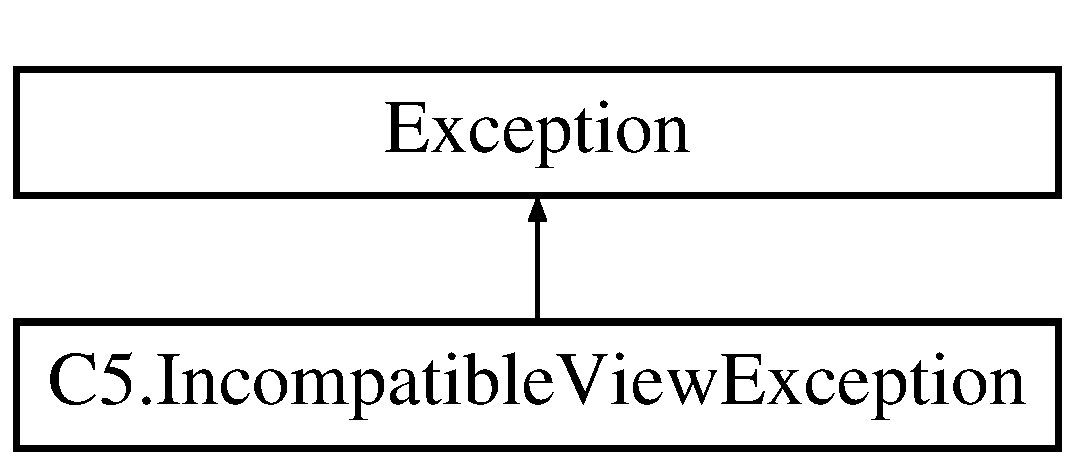
\includegraphics[height=2.000000cm]{class_c5_1_1_incompatible_view_exception}
\end{center}
\end{figure}
\subsection*{Public Member Functions}
\begin{DoxyCompactItemize}
\item 
\hyperlink{class_c5_1_1_incompatible_view_exception_a2213279b2e6743b6355cc0ad598393b0}{Incompatible\+View\+Exception} ()
\begin{DoxyCompactList}\small\item\em Create a simple exception with no further explanation. \end{DoxyCompactList}\item 
\hyperlink{class_c5_1_1_incompatible_view_exception_a61a8a3695642eaa2bc67c47ec245490b}{Incompatible\+View\+Exception} (string message)
\begin{DoxyCompactList}\small\item\em Create the exception with an explanation of the reason. \end{DoxyCompactList}\end{DoxyCompactItemize}


\subsection{Detailed Description}
An exception thrown by operations on a list that expects an argument that is a view on the same underlying list. 



\subsection{Constructor \& Destructor Documentation}
\hypertarget{class_c5_1_1_incompatible_view_exception_a2213279b2e6743b6355cc0ad598393b0}{}\index{C5\+::\+Incompatible\+View\+Exception@{C5\+::\+Incompatible\+View\+Exception}!Incompatible\+View\+Exception@{Incompatible\+View\+Exception}}
\index{Incompatible\+View\+Exception@{Incompatible\+View\+Exception}!C5\+::\+Incompatible\+View\+Exception@{C5\+::\+Incompatible\+View\+Exception}}
\subsubsection[{Incompatible\+View\+Exception()}]{\setlength{\rightskip}{0pt plus 5cm}C5.\+Incompatible\+View\+Exception.\+Incompatible\+View\+Exception (
\begin{DoxyParamCaption}
{}
\end{DoxyParamCaption}
)}\label{class_c5_1_1_incompatible_view_exception_a2213279b2e6743b6355cc0ad598393b0}


Create a simple exception with no further explanation. 

\hypertarget{class_c5_1_1_incompatible_view_exception_a61a8a3695642eaa2bc67c47ec245490b}{}\index{C5\+::\+Incompatible\+View\+Exception@{C5\+::\+Incompatible\+View\+Exception}!Incompatible\+View\+Exception@{Incompatible\+View\+Exception}}
\index{Incompatible\+View\+Exception@{Incompatible\+View\+Exception}!C5\+::\+Incompatible\+View\+Exception@{C5\+::\+Incompatible\+View\+Exception}}
\subsubsection[{Incompatible\+View\+Exception(string message)}]{\setlength{\rightskip}{0pt plus 5cm}C5.\+Incompatible\+View\+Exception.\+Incompatible\+View\+Exception (
\begin{DoxyParamCaption}
\item[{string}]{message}
\end{DoxyParamCaption}
)}\label{class_c5_1_1_incompatible_view_exception_a61a8a3695642eaa2bc67c47ec245490b}


Create the exception with an explanation of the reason. 


\begin{DoxyParams}{Parameters}
{\em message} & \\
\hline
\end{DoxyParams}


The documentation for this class was generated from the following file\+:\begin{DoxyCompactItemize}
\item 
C\+:/\+Users/rasmusl/\+Source/\+Repos/\+C5/\+C5/\hyperlink{_exceptions_8cs}{Exceptions.\+cs}\end{DoxyCompactItemize}

\hypertarget{class_c5_1_1_internal_exception}{}\section{C5.\+Internal\+Exception Class Reference}
\label{class_c5_1_1_internal_exception}\index{C5.\+Internal\+Exception@{C5.\+Internal\+Exception}}


An exception to throw from library code when an internal inconsistency is encountered.  


Inheritance diagram for C5.\+Internal\+Exception\+:\begin{figure}[H]
\begin{center}
\leavevmode
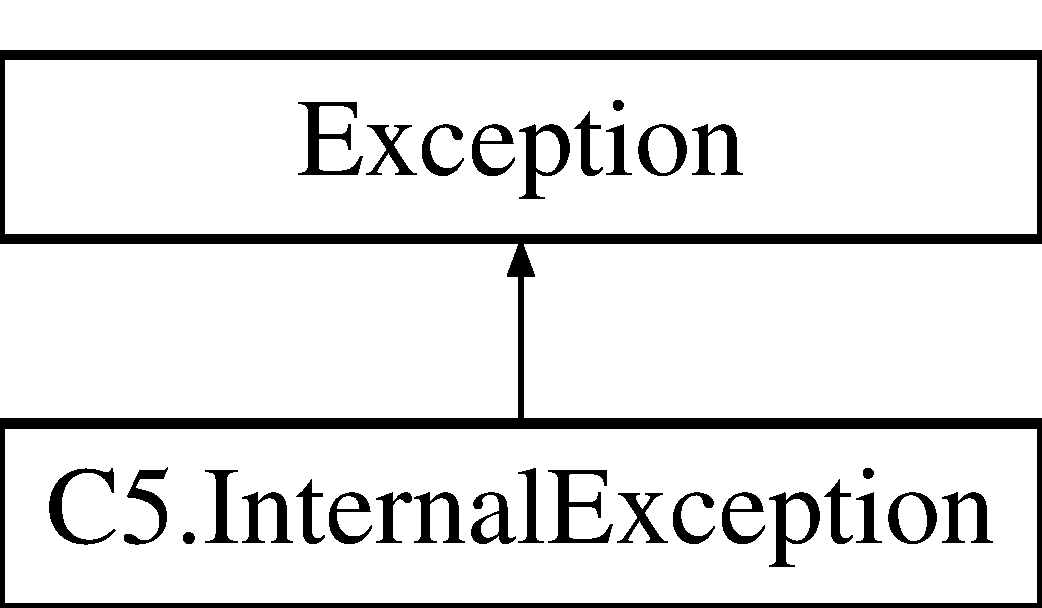
\includegraphics[height=2.000000cm]{class_c5_1_1_internal_exception}
\end{center}
\end{figure}


\subsection{Detailed Description}
An exception to throw from library code when an internal inconsistency is encountered. 



The documentation for this class was generated from the following file\+:\begin{DoxyCompactItemize}
\item 
C\+:/\+Users/rasmusl/\+Source/\+Repos/\+C5/\+C5/\hyperlink{_exceptions_8cs}{Exceptions.\+cs}\end{DoxyCompactItemize}

\hypertarget{class_c5_1_1_interval_heap}{}\section{C5.\+Interval\+Heap$<$ T $>$ Class Template Reference}
\label{class_c5_1_1_interval_heap}\index{C5.\+Interval\+Heap$<$ T $>$@{C5.\+Interval\+Heap$<$ T $>$}}


A priority queue class based on an interval heap data structure.  


Inheritance diagram for C5.\+Interval\+Heap$<$ T $>$\+:\begin{figure}[H]
\begin{center}
\leavevmode
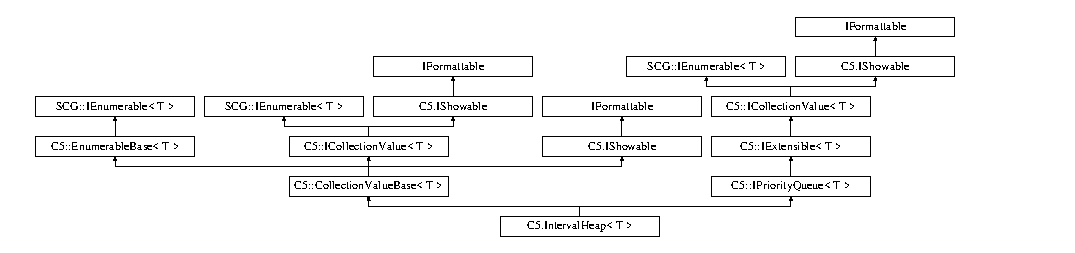
\includegraphics[height=2.947368cm]{class_c5_1_1_interval_heap}
\end{center}
\end{figure}
\subsection*{Public Member Functions}
\begin{DoxyCompactItemize}
\item 
\hyperlink{class_c5_1_1_interval_heap_a5a6140a981bbc3f40b101a26dee6c37f}{Interval\+Heap} ()
\begin{DoxyCompactList}\small\item\em Create an interval heap with natural item comparer and default initial capacity (16) \end{DoxyCompactList}\item 
\hyperlink{class_c5_1_1_interval_heap_a94962594feb3b88e0cd87ad2397df4ed}{Interval\+Heap} (S\+C\+G.\+I\+Comparer$<$ T $>$ comparer)
\begin{DoxyCompactList}\small\item\em Create an interval heap with external item comparer and default initial capacity (16) \end{DoxyCompactList}\item 
\hyperlink{class_c5_1_1_interval_heap_ae7bdfcb5955687d26fc5a380c89256eb}{Interval\+Heap} (int capacity)
\begin{DoxyCompactList}\small\item\em Create an interval heap with natural item comparer and prescribed initial capacity \end{DoxyCompactList}\item 
\hyperlink{class_c5_1_1_interval_heap_a4259a4d0b543370844e066dd9a165c49}{Interval\+Heap} (int capacity, S\+C\+G.\+I\+Comparer$<$ T $>$ comparer)
\begin{DoxyCompactList}\small\item\em Create an interval heap with external item comparer and prescribed initial capacity \end{DoxyCompactList}\item 
T \hyperlink{class_c5_1_1_interval_heap_ad4671adf7daad4e8b6711c0a9a5663fe}{Find\+Min} ()
\begin{DoxyCompactList}\small\item\em Find the current least item of this priority queue. 
\begin{DoxyExceptions}{Exceptions}
{\em \hyperlink{class_c5_1_1_no_such_item_exception}{No\+Such\+Item\+Exception}} & if queue is empty \\
\hline
\end{DoxyExceptions}
\end{DoxyCompactList}\item 
T \hyperlink{class_c5_1_1_interval_heap_a63772295b880e38f9ef5c2469a687770}{Delete\+Min} ()
\begin{DoxyCompactList}\small\item\em Remove the least item from this priority queue. 
\begin{DoxyExceptions}{Exceptions}
{\em \hyperlink{class_c5_1_1_no_such_item_exception}{No\+Such\+Item\+Exception}} & if queue is empty \\
\hline
\end{DoxyExceptions}
\end{DoxyCompactList}\item 
T \hyperlink{class_c5_1_1_interval_heap_abda450e3da23bc35d0db7f4f0dd91d00}{Find\+Max} ()
\begin{DoxyCompactList}\small\item\em Find the current largest item of this priority queue. 
\begin{DoxyExceptions}{Exceptions}
{\em \hyperlink{class_c5_1_1_no_such_item_exception}{No\+Such\+Item\+Exception}} & if queue is empty \\
\hline
\end{DoxyExceptions}
\end{DoxyCompactList}\item 
T \hyperlink{class_c5_1_1_interval_heap_a487241b83be6837692408542c7cfb6b5}{Delete\+Max} ()
\begin{DoxyCompactList}\small\item\em Remove the largest item from this priority queue. 
\begin{DoxyExceptions}{Exceptions}
{\em \hyperlink{class_c5_1_1_no_such_item_exception}{No\+Such\+Item\+Exception}} & if queue is empty \\
\hline
\end{DoxyExceptions}
\end{DoxyCompactList}\item 
bool \hyperlink{class_c5_1_1_interval_heap_ab7c3c348aa1f0f2723dd0a533e1c458f}{Add} (T item)
\begin{DoxyCompactList}\small\item\em Add an item to this priority queue. \end{DoxyCompactList}\item 
void \hyperlink{class_c5_1_1_interval_heap_abe5fb2f06b082e4fec00dc454cd31ed8}{Add\+All} (S\+C\+G.\+I\+Enumerable$<$ T $>$ items)
\begin{DoxyCompactList}\small\item\em Add the elements from another collection with a more specialized item type to this collection. \end{DoxyCompactList}\item 
override T \hyperlink{class_c5_1_1_interval_heap_a0d5fe1b0687d6ef002a17c6e46900772}{Choose} ()
\begin{DoxyCompactList}\small\item\em Choose some item of this collection. \end{DoxyCompactList}\item 
override S\+C\+G.\+I\+Enumerator$<$ T $>$ \hyperlink{class_c5_1_1_interval_heap_a09556ba66252a46d94456587bc877561}{Get\+Enumerator} ()
\begin{DoxyCompactList}\small\item\em Create an enumerator for the collection \end{DoxyCompactList}\item 
bool \hyperlink{class_c5_1_1_interval_heap_a9682f00247167989ae132c26ded9f600}{Check} ()
\begin{DoxyCompactList}\small\item\em Check the integrity of the internal data structures of this collection. Only avaliable in D\+E\+B\+U\+G builds??? \end{DoxyCompactList}\item 
bool \hyperlink{class_c5_1_1_interval_heap_abaae4e91221233de39a8062ae7c89402}{Find} (\hyperlink{interface_c5_1_1_i_priority_queue_handle}{I\+Priority\+Queue\+Handle}$<$ T $>$ handle, out T item)
\begin{DoxyCompactList}\small\item\em Check safely if a handle is valid for this queue and if so, report the corresponding queue item. \end{DoxyCompactList}\item 
bool \hyperlink{class_c5_1_1_interval_heap_a4ea1fbf9bb6c727fc83a033e311074ec}{Add} (ref \hyperlink{interface_c5_1_1_i_priority_queue_handle}{I\+Priority\+Queue\+Handle}$<$ T $>$ handle, T item)
\begin{DoxyCompactList}\small\item\em Add an item to the priority queue, receiving a handle for the item in the queue, or reusing an already existing handle. \end{DoxyCompactList}\item 
T \hyperlink{class_c5_1_1_interval_heap_a3f9868407c50d789c85e998448e50114}{Delete} (\hyperlink{interface_c5_1_1_i_priority_queue_handle}{I\+Priority\+Queue\+Handle}$<$ T $>$ handle)
\begin{DoxyCompactList}\small\item\em Delete an item with a handle from a priority queue. \end{DoxyCompactList}\item 
T \hyperlink{class_c5_1_1_interval_heap_abfc2e592410f83b10f7feb82bcbd53db}{Replace} (\hyperlink{interface_c5_1_1_i_priority_queue_handle}{I\+Priority\+Queue\+Handle}$<$ T $>$ handle, T item)
\begin{DoxyCompactList}\small\item\em Replace an item with a handle in a priority queue with a new item. Typically used for changing the priority of some queued object. \end{DoxyCompactList}\item 
T \hyperlink{class_c5_1_1_interval_heap_a3b14d4af51572b295c9eebdf880ed493}{Find\+Min} (out \hyperlink{interface_c5_1_1_i_priority_queue_handle}{I\+Priority\+Queue\+Handle}$<$ T $>$ handle)
\begin{DoxyCompactList}\small\item\em Find the current least item of this priority queue. \end{DoxyCompactList}\item 
T \hyperlink{class_c5_1_1_interval_heap_aeb97ce7d763c7e3707251de9f76071aa}{Find\+Max} (out \hyperlink{interface_c5_1_1_i_priority_queue_handle}{I\+Priority\+Queue\+Handle}$<$ T $>$ handle)
\begin{DoxyCompactList}\small\item\em Find the current largest item of this priority queue. \end{DoxyCompactList}\item 
T \hyperlink{class_c5_1_1_interval_heap_a3b605362b2ab7bf2268383be00015f6d}{Delete\+Min} (out \hyperlink{interface_c5_1_1_i_priority_queue_handle}{I\+Priority\+Queue\+Handle}$<$ T $>$ handle)
\begin{DoxyCompactList}\small\item\em Remove the least item from this priority queue. \end{DoxyCompactList}\item 
T \hyperlink{class_c5_1_1_interval_heap_ac5446ec37bcee1e0f117fbbe566f6386}{Delete\+Max} (out \hyperlink{interface_c5_1_1_i_priority_queue_handle}{I\+Priority\+Queue\+Handle}$<$ T $>$ handle)
\begin{DoxyCompactList}\small\item\em Remove the largest item from this priority queue. \end{DoxyCompactList}\end{DoxyCompactItemize}
\subsection*{Properties}
\begin{DoxyCompactItemize}
\item 
override \hyperlink{namespace_c5_a9143bfd561fffa025d21561674758008}{Event\+Type\+Enum} \hyperlink{class_c5_1_1_interval_heap_aea675c936b84378eaa72d208a80605dd}{Listenable\+Events}\hspace{0.3cm}{\ttfamily  \mbox{[}get\mbox{]}}
\item 
S\+C\+G.\+I\+Comparer$<$ T $>$ \hyperlink{class_c5_1_1_interval_heap_a0da8aaabae59ac97119bff56d16e6a87}{Comparer}\hspace{0.3cm}{\ttfamily  \mbox{[}get\mbox{]}}
\begin{DoxyCompactList}\small\item\em The comparer object supplied at creation time for this collection \end{DoxyCompactList}\item 
bool \hyperlink{class_c5_1_1_interval_heap_a0c7d60732701b904a277b1c776224fbf}{Is\+Read\+Only}\hspace{0.3cm}{\ttfamily  \mbox{[}get\mbox{]}}
\begin{DoxyCompactList}\small\item\em If true any call of an updating operation will throw an \end{DoxyCompactList}\item 
bool \hyperlink{class_c5_1_1_interval_heap_a3f04b4e3b21b55967adcb6cf7f3252dc}{Allows\+Duplicates}\hspace{0.3cm}{\ttfamily  \mbox{[}get\mbox{]}}
\item 
virtual S\+C\+G.\+I\+Equality\+Comparer$<$ T $>$ \hyperlink{class_c5_1_1_interval_heap_a0c8af0d3e8f557d3e083513a2774676a}{Equality\+Comparer}\hspace{0.3cm}{\ttfamily  \mbox{[}get\mbox{]}}
\begin{DoxyCompactList}\small\item\em Value is null since this collection has no equality concept for its items. \end{DoxyCompactList}\item 
virtual bool \hyperlink{class_c5_1_1_interval_heap_a7e944979e8700149ef1605b5ff7019e9}{Duplicates\+By\+Counting}\hspace{0.3cm}{\ttfamily  \mbox{[}get\mbox{]}}
\begin{DoxyCompactList}\small\item\em By convention this is true for any collection with set semantics. \end{DoxyCompactList}\item 
override bool \hyperlink{class_c5_1_1_interval_heap_aa6146324a58bb879c502a9f1cfb483a8}{Is\+Empty}\hspace{0.3cm}{\ttfamily  \mbox{[}get\mbox{]}}
\item 
override int \hyperlink{class_c5_1_1_interval_heap_a4db5c619c65ba918015da4cd45f7ba8d}{Count}\hspace{0.3cm}{\ttfamily  \mbox{[}get\mbox{]}}
\item 
override \hyperlink{namespace_c5_a615ba88dcdaa8d5a3c5f833a73d7fad6}{Speed} \hyperlink{class_c5_1_1_interval_heap_a33d630a81c86d10cf5cff931662f3808}{Count\+Speed}\hspace{0.3cm}{\ttfamily  \mbox{[}get\mbox{]}}
\begin{DoxyCompactList}\small\item\em The value is symbolic indicating the type of asymptotic complexity in terms of the size of this collection (worst-\/case or amortized as relevant). \end{DoxyCompactList}\item 
T \hyperlink{class_c5_1_1_interval_heap_a91e32b822986bd74b9e3862a767d0c13}{this\mbox{[}\+I\+Priority\+Queue\+Handle$<$ T $>$ handle\mbox{]}}\hspace{0.3cm}{\ttfamily  \mbox{[}get, set\mbox{]}}
\begin{DoxyCompactList}\small\item\em Get or set the item corresponding to a handle. \end{DoxyCompactList}\end{DoxyCompactItemize}
\subsection*{Additional Inherited Members}


\subsection{Detailed Description}
A priority queue class based on an interval heap data structure. 


\begin{DoxyTemplParams}{Template Parameters}
{\em T} & The item type\\
\hline
\end{DoxyTemplParams}


\subsection{Constructor \& Destructor Documentation}
\hypertarget{class_c5_1_1_interval_heap_a5a6140a981bbc3f40b101a26dee6c37f}{}\index{C5\+::\+Interval\+Heap@{C5\+::\+Interval\+Heap}!Interval\+Heap@{Interval\+Heap}}
\index{Interval\+Heap@{Interval\+Heap}!C5\+::\+Interval\+Heap@{C5\+::\+Interval\+Heap}}
\subsubsection[{Interval\+Heap()}]{\setlength{\rightskip}{0pt plus 5cm}{\bf C5.\+Interval\+Heap}$<$ T $>$.{\bf Interval\+Heap} (
\begin{DoxyParamCaption}
{}
\end{DoxyParamCaption}
)}\label{class_c5_1_1_interval_heap_a5a6140a981bbc3f40b101a26dee6c37f}


Create an interval heap with natural item comparer and default initial capacity (16) 

\hypertarget{class_c5_1_1_interval_heap_a94962594feb3b88e0cd87ad2397df4ed}{}\index{C5\+::\+Interval\+Heap@{C5\+::\+Interval\+Heap}!Interval\+Heap@{Interval\+Heap}}
\index{Interval\+Heap@{Interval\+Heap}!C5\+::\+Interval\+Heap@{C5\+::\+Interval\+Heap}}
\subsubsection[{Interval\+Heap(\+S\+C\+G.\+I\+Comparer$<$ T $>$ comparer)}]{\setlength{\rightskip}{0pt plus 5cm}{\bf C5.\+Interval\+Heap}$<$ T $>$.{\bf Interval\+Heap} (
\begin{DoxyParamCaption}
\item[{S\+C\+G.\+I\+Comparer$<$ T $>$}]{comparer}
\end{DoxyParamCaption}
)}\label{class_c5_1_1_interval_heap_a94962594feb3b88e0cd87ad2397df4ed}


Create an interval heap with external item comparer and default initial capacity (16) 


\begin{DoxyParams}{Parameters}
{\em comparer} & The external comparer\\
\hline
\end{DoxyParams}
\hypertarget{class_c5_1_1_interval_heap_ae7bdfcb5955687d26fc5a380c89256eb}{}\index{C5\+::\+Interval\+Heap@{C5\+::\+Interval\+Heap}!Interval\+Heap@{Interval\+Heap}}
\index{Interval\+Heap@{Interval\+Heap}!C5\+::\+Interval\+Heap@{C5\+::\+Interval\+Heap}}
\subsubsection[{Interval\+Heap(int capacity)}]{\setlength{\rightskip}{0pt plus 5cm}{\bf C5.\+Interval\+Heap}$<$ T $>$.{\bf Interval\+Heap} (
\begin{DoxyParamCaption}
\item[{int}]{capacity}
\end{DoxyParamCaption}
)}\label{class_c5_1_1_interval_heap_ae7bdfcb5955687d26fc5a380c89256eb}


Create an interval heap with natural item comparer and prescribed initial capacity 


\begin{DoxyParams}{Parameters}
{\em capacity} & The initial capacity\\
\hline
\end{DoxyParams}
\hypertarget{class_c5_1_1_interval_heap_a4259a4d0b543370844e066dd9a165c49}{}\index{C5\+::\+Interval\+Heap@{C5\+::\+Interval\+Heap}!Interval\+Heap@{Interval\+Heap}}
\index{Interval\+Heap@{Interval\+Heap}!C5\+::\+Interval\+Heap@{C5\+::\+Interval\+Heap}}
\subsubsection[{Interval\+Heap(int capacity, S\+C\+G.\+I\+Comparer$<$ T $>$ comparer)}]{\setlength{\rightskip}{0pt plus 5cm}{\bf C5.\+Interval\+Heap}$<$ T $>$.{\bf Interval\+Heap} (
\begin{DoxyParamCaption}
\item[{int}]{capacity, }
\item[{S\+C\+G.\+I\+Comparer$<$ T $>$}]{comparer}
\end{DoxyParamCaption}
)}\label{class_c5_1_1_interval_heap_a4259a4d0b543370844e066dd9a165c49}


Create an interval heap with external item comparer and prescribed initial capacity 


\begin{DoxyParams}{Parameters}
{\em comparer} & The external comparer\\
\hline
{\em capacity} & The initial capacity\\
\hline
\end{DoxyParams}


\subsection{Member Function Documentation}
\hypertarget{class_c5_1_1_interval_heap_ab7c3c348aa1f0f2723dd0a533e1c458f}{}\index{C5\+::\+Interval\+Heap@{C5\+::\+Interval\+Heap}!Add@{Add}}
\index{Add@{Add}!C5\+::\+Interval\+Heap@{C5\+::\+Interval\+Heap}}
\subsubsection[{Add(\+T item)}]{\setlength{\rightskip}{0pt plus 5cm}bool {\bf C5.\+Interval\+Heap}$<$ T $>$.Add (
\begin{DoxyParamCaption}
\item[{T}]{item}
\end{DoxyParamCaption}
)}\label{class_c5_1_1_interval_heap_ab7c3c348aa1f0f2723dd0a533e1c458f}


Add an item to this priority queue. 


\begin{DoxyParams}{Parameters}
{\em item} & The item to add.\\
\hline
\end{DoxyParams}
\begin{DoxyReturn}{Returns}
True
\end{DoxyReturn}


Implements \hyperlink{interface_c5_1_1_i_extensible_acfe8d39605927db1aff0572e2b5c1089}{C5.\+I\+Extensible$<$ T $>$}.

\hypertarget{class_c5_1_1_interval_heap_a4ea1fbf9bb6c727fc83a033e311074ec}{}\index{C5\+::\+Interval\+Heap@{C5\+::\+Interval\+Heap}!Add@{Add}}
\index{Add@{Add}!C5\+::\+Interval\+Heap@{C5\+::\+Interval\+Heap}}
\subsubsection[{Add(ref I\+Priority\+Queue\+Handle$<$ T $>$ handle, T item)}]{\setlength{\rightskip}{0pt plus 5cm}bool {\bf C5.\+Interval\+Heap}$<$ T $>$.Add (
\begin{DoxyParamCaption}
\item[{ref {\bf I\+Priority\+Queue\+Handle}$<$ T $>$}]{handle, }
\item[{T}]{item}
\end{DoxyParamCaption}
)}\label{class_c5_1_1_interval_heap_a4ea1fbf9bb6c727fc83a033e311074ec}


Add an item to the priority queue, receiving a handle for the item in the queue, or reusing an already existing handle. 


\begin{DoxyParams}{Parameters}
{\em handle} & On output\+: a handle for the added item. On input\+: null for allocating a new handle, an invalid handle for reuse. A handle for reuse must be compatible with this priority queue, by being created by a priority queue of the same runtime type, but not necessarily the same priority queue object.\\
\hline
{\em item} & The item to add.\\
\hline
\end{DoxyParams}
\begin{DoxyReturn}{Returns}
True since item will always be added unless the call throws an exception.
\end{DoxyReturn}


Implements \hyperlink{interface_c5_1_1_i_priority_queue_ac90f40246d54cb28935bf89d9e0c9c72}{C5.\+I\+Priority\+Queue$<$ T $>$}.

\hypertarget{class_c5_1_1_interval_heap_abe5fb2f06b082e4fec00dc454cd31ed8}{}\index{C5\+::\+Interval\+Heap@{C5\+::\+Interval\+Heap}!Add\+All@{Add\+All}}
\index{Add\+All@{Add\+All}!C5\+::\+Interval\+Heap@{C5\+::\+Interval\+Heap}}
\subsubsection[{Add\+All(\+S\+C\+G.\+I\+Enumerable$<$ T $>$ items)}]{\setlength{\rightskip}{0pt plus 5cm}void {\bf C5.\+Interval\+Heap}$<$ T $>$.Add\+All (
\begin{DoxyParamCaption}
\item[{S\+C\+G.\+I\+Enumerable$<$ T $>$}]{items}
\end{DoxyParamCaption}
)}\label{class_c5_1_1_interval_heap_abe5fb2f06b082e4fec00dc454cd31ed8}


Add the elements from another collection with a more specialized item type to this collection. 


\begin{DoxyParams}{Parameters}
{\em items} & The items to add\\
\hline
\end{DoxyParams}


Implements \hyperlink{interface_c5_1_1_i_extensible_a1fb4d50c5b340e60303da72e9d0ede6e}{C5.\+I\+Extensible$<$ T $>$}.

\hypertarget{class_c5_1_1_interval_heap_a9682f00247167989ae132c26ded9f600}{}\index{C5\+::\+Interval\+Heap@{C5\+::\+Interval\+Heap}!Check@{Check}}
\index{Check@{Check}!C5\+::\+Interval\+Heap@{C5\+::\+Interval\+Heap}}
\subsubsection[{Check()}]{\setlength{\rightskip}{0pt plus 5cm}bool {\bf C5.\+Interval\+Heap}$<$ T $>$.Check (
\begin{DoxyParamCaption}
{}
\end{DoxyParamCaption}
)}\label{class_c5_1_1_interval_heap_a9682f00247167989ae132c26ded9f600}


Check the integrity of the internal data structures of this collection. Only avaliable in D\+E\+B\+U\+G builds??? 

\begin{DoxyReturn}{Returns}
True if check does not fail.
\end{DoxyReturn}


Implements \hyperlink{interface_c5_1_1_i_extensible_aeeb6b87af61e455df42d68834d711bcb}{C5.\+I\+Extensible$<$ T $>$}.

\hypertarget{class_c5_1_1_interval_heap_a0d5fe1b0687d6ef002a17c6e46900772}{}\index{C5\+::\+Interval\+Heap@{C5\+::\+Interval\+Heap}!Choose@{Choose}}
\index{Choose@{Choose}!C5\+::\+Interval\+Heap@{C5\+::\+Interval\+Heap}}
\subsubsection[{Choose()}]{\setlength{\rightskip}{0pt plus 5cm}override T {\bf C5.\+Interval\+Heap}$<$ T $>$.Choose (
\begin{DoxyParamCaption}
{}
\end{DoxyParamCaption}
)\hspace{0.3cm}{\ttfamily [virtual]}}\label{class_c5_1_1_interval_heap_a0d5fe1b0687d6ef002a17c6e46900772}


Choose some item of this collection. 


\begin{DoxyExceptions}{Exceptions}
{\em \hyperlink{class_c5_1_1_no_such_item_exception}{No\+Such\+Item\+Exception}} & if collection is empty.\\
\hline
\end{DoxyExceptions}
\begin{DoxyReturn}{Returns}

\end{DoxyReturn}


Implements \hyperlink{class_c5_1_1_collection_value_base_ad7b8bd01dfd7ea8480a972f02a81608b}{C5.\+Collection\+Value\+Base$<$ T $>$}.

\hypertarget{class_c5_1_1_interval_heap_a3f9868407c50d789c85e998448e50114}{}\index{C5\+::\+Interval\+Heap@{C5\+::\+Interval\+Heap}!Delete@{Delete}}
\index{Delete@{Delete}!C5\+::\+Interval\+Heap@{C5\+::\+Interval\+Heap}}
\subsubsection[{Delete(\+I\+Priority\+Queue\+Handle$<$ T $>$ handle)}]{\setlength{\rightskip}{0pt plus 5cm}T {\bf C5.\+Interval\+Heap}$<$ T $>$.Delete (
\begin{DoxyParamCaption}
\item[{{\bf I\+Priority\+Queue\+Handle}$<$ T $>$}]{handle}
\end{DoxyParamCaption}
)}\label{class_c5_1_1_interval_heap_a3f9868407c50d789c85e998448e50114}


Delete an item with a handle from a priority queue. 


\begin{DoxyExceptions}{Exceptions}
{\em \hyperlink{class_c5_1_1_invalid_priority_queue_handle_exception}{Invalid\+Priority\+Queue\+Handle\+Exception}} & if the handle is invalid\\
\hline
\end{DoxyExceptions}

\begin{DoxyParams}{Parameters}
{\em handle} & The handle for the item. The handle will be invalidated, but reusable.\\
\hline
\end{DoxyParams}
\begin{DoxyReturn}{Returns}
The deleted item
\end{DoxyReturn}


Implements \hyperlink{interface_c5_1_1_i_priority_queue_a8b1272ae3287f72eeece44d17a9c2eff}{C5.\+I\+Priority\+Queue$<$ T $>$}.

\hypertarget{class_c5_1_1_interval_heap_a487241b83be6837692408542c7cfb6b5}{}\index{C5\+::\+Interval\+Heap@{C5\+::\+Interval\+Heap}!Delete\+Max@{Delete\+Max}}
\index{Delete\+Max@{Delete\+Max}!C5\+::\+Interval\+Heap@{C5\+::\+Interval\+Heap}}
\subsubsection[{Delete\+Max()}]{\setlength{\rightskip}{0pt plus 5cm}T {\bf C5.\+Interval\+Heap}$<$ T $>$.Delete\+Max (
\begin{DoxyParamCaption}
{}
\end{DoxyParamCaption}
)}\label{class_c5_1_1_interval_heap_a487241b83be6837692408542c7cfb6b5}


Remove the largest item from this priority queue. 
\begin{DoxyExceptions}{Exceptions}
{\em \hyperlink{class_c5_1_1_no_such_item_exception}{No\+Such\+Item\+Exception}} & if queue is empty \\
\hline
\end{DoxyExceptions}


\begin{DoxyReturn}{Returns}
The removed item.
\end{DoxyReturn}


Implements \hyperlink{interface_c5_1_1_i_priority_queue_a8f728da5fbc6ae1bb4b2941d51885d69}{C5.\+I\+Priority\+Queue$<$ T $>$}.

\hypertarget{class_c5_1_1_interval_heap_ac5446ec37bcee1e0f117fbbe566f6386}{}\index{C5\+::\+Interval\+Heap@{C5\+::\+Interval\+Heap}!Delete\+Max@{Delete\+Max}}
\index{Delete\+Max@{Delete\+Max}!C5\+::\+Interval\+Heap@{C5\+::\+Interval\+Heap}}
\subsubsection[{Delete\+Max(out I\+Priority\+Queue\+Handle$<$ T $>$ handle)}]{\setlength{\rightskip}{0pt plus 5cm}T {\bf C5.\+Interval\+Heap}$<$ T $>$.Delete\+Max (
\begin{DoxyParamCaption}
\item[{out {\bf I\+Priority\+Queue\+Handle}$<$ T $>$}]{handle}
\end{DoxyParamCaption}
)}\label{class_c5_1_1_interval_heap_ac5446ec37bcee1e0f117fbbe566f6386}


Remove the largest item from this priority queue. 


\begin{DoxyParams}{Parameters}
{\em handle} & On return\+: the handle of the removed item.\\
\hline
\end{DoxyParams}
\begin{DoxyReturn}{Returns}
The removed item.
\end{DoxyReturn}


Implements \hyperlink{interface_c5_1_1_i_priority_queue_ae6b746354d02c65d0435040682baf0c9}{C5.\+I\+Priority\+Queue$<$ T $>$}.

\hypertarget{class_c5_1_1_interval_heap_a63772295b880e38f9ef5c2469a687770}{}\index{C5\+::\+Interval\+Heap@{C5\+::\+Interval\+Heap}!Delete\+Min@{Delete\+Min}}
\index{Delete\+Min@{Delete\+Min}!C5\+::\+Interval\+Heap@{C5\+::\+Interval\+Heap}}
\subsubsection[{Delete\+Min()}]{\setlength{\rightskip}{0pt plus 5cm}T {\bf C5.\+Interval\+Heap}$<$ T $>$.Delete\+Min (
\begin{DoxyParamCaption}
{}
\end{DoxyParamCaption}
)}\label{class_c5_1_1_interval_heap_a63772295b880e38f9ef5c2469a687770}


Remove the least item from this priority queue. 
\begin{DoxyExceptions}{Exceptions}
{\em \hyperlink{class_c5_1_1_no_such_item_exception}{No\+Such\+Item\+Exception}} & if queue is empty \\
\hline
\end{DoxyExceptions}


\begin{DoxyReturn}{Returns}
The removed item.
\end{DoxyReturn}


Implements \hyperlink{interface_c5_1_1_i_priority_queue_a278dfa42e80291ba82122f174895dd77}{C5.\+I\+Priority\+Queue$<$ T $>$}.

\hypertarget{class_c5_1_1_interval_heap_a3b605362b2ab7bf2268383be00015f6d}{}\index{C5\+::\+Interval\+Heap@{C5\+::\+Interval\+Heap}!Delete\+Min@{Delete\+Min}}
\index{Delete\+Min@{Delete\+Min}!C5\+::\+Interval\+Heap@{C5\+::\+Interval\+Heap}}
\subsubsection[{Delete\+Min(out I\+Priority\+Queue\+Handle$<$ T $>$ handle)}]{\setlength{\rightskip}{0pt plus 5cm}T {\bf C5.\+Interval\+Heap}$<$ T $>$.Delete\+Min (
\begin{DoxyParamCaption}
\item[{out {\bf I\+Priority\+Queue\+Handle}$<$ T $>$}]{handle}
\end{DoxyParamCaption}
)}\label{class_c5_1_1_interval_heap_a3b605362b2ab7bf2268383be00015f6d}


Remove the least item from this priority queue. 


\begin{DoxyParams}{Parameters}
{\em handle} & On return\+: the handle of the removed item.\\
\hline
\end{DoxyParams}
\begin{DoxyReturn}{Returns}
The removed item.
\end{DoxyReturn}


Implements \hyperlink{interface_c5_1_1_i_priority_queue_a3aca77813a8c6d30de8bc8d8ff734de0}{C5.\+I\+Priority\+Queue$<$ T $>$}.

\hypertarget{class_c5_1_1_interval_heap_abaae4e91221233de39a8062ae7c89402}{}\index{C5\+::\+Interval\+Heap@{C5\+::\+Interval\+Heap}!Find@{Find}}
\index{Find@{Find}!C5\+::\+Interval\+Heap@{C5\+::\+Interval\+Heap}}
\subsubsection[{Find(\+I\+Priority\+Queue\+Handle$<$ T $>$ handle, out T item)}]{\setlength{\rightskip}{0pt plus 5cm}bool {\bf C5.\+Interval\+Heap}$<$ T $>$.Find (
\begin{DoxyParamCaption}
\item[{{\bf I\+Priority\+Queue\+Handle}$<$ T $>$}]{handle, }
\item[{out T}]{item}
\end{DoxyParamCaption}
)}\label{class_c5_1_1_interval_heap_abaae4e91221233de39a8062ae7c89402}


Check safely if a handle is valid for this queue and if so, report the corresponding queue item. 


\begin{DoxyParams}{Parameters}
{\em handle} & The handle to check\\
\hline
{\em item} & If the handle is valid this will contain the corresponding item on output.\\
\hline
\end{DoxyParams}
\begin{DoxyReturn}{Returns}
True if the handle is valid.
\end{DoxyReturn}


Implements \hyperlink{interface_c5_1_1_i_priority_queue_a4f8bac3647b3b668939a0e9c34c158e5}{C5.\+I\+Priority\+Queue$<$ T $>$}.

\hypertarget{class_c5_1_1_interval_heap_abda450e3da23bc35d0db7f4f0dd91d00}{}\index{C5\+::\+Interval\+Heap@{C5\+::\+Interval\+Heap}!Find\+Max@{Find\+Max}}
\index{Find\+Max@{Find\+Max}!C5\+::\+Interval\+Heap@{C5\+::\+Interval\+Heap}}
\subsubsection[{Find\+Max()}]{\setlength{\rightskip}{0pt plus 5cm}T {\bf C5.\+Interval\+Heap}$<$ T $>$.Find\+Max (
\begin{DoxyParamCaption}
{}
\end{DoxyParamCaption}
)}\label{class_c5_1_1_interval_heap_abda450e3da23bc35d0db7f4f0dd91d00}


Find the current largest item of this priority queue. 
\begin{DoxyExceptions}{Exceptions}
{\em \hyperlink{class_c5_1_1_no_such_item_exception}{No\+Such\+Item\+Exception}} & if queue is empty \\
\hline
\end{DoxyExceptions}


\begin{DoxyReturn}{Returns}
The largest item.
\end{DoxyReturn}


Implements \hyperlink{interface_c5_1_1_i_priority_queue_ab510a95957edce0bb68aedd85abb73f8}{C5.\+I\+Priority\+Queue$<$ T $>$}.

\hypertarget{class_c5_1_1_interval_heap_aeb97ce7d763c7e3707251de9f76071aa}{}\index{C5\+::\+Interval\+Heap@{C5\+::\+Interval\+Heap}!Find\+Max@{Find\+Max}}
\index{Find\+Max@{Find\+Max}!C5\+::\+Interval\+Heap@{C5\+::\+Interval\+Heap}}
\subsubsection[{Find\+Max(out I\+Priority\+Queue\+Handle$<$ T $>$ handle)}]{\setlength{\rightskip}{0pt plus 5cm}T {\bf C5.\+Interval\+Heap}$<$ T $>$.Find\+Max (
\begin{DoxyParamCaption}
\item[{out {\bf I\+Priority\+Queue\+Handle}$<$ T $>$}]{handle}
\end{DoxyParamCaption}
)}\label{class_c5_1_1_interval_heap_aeb97ce7d763c7e3707251de9f76071aa}


Find the current largest item of this priority queue. 


\begin{DoxyParams}{Parameters}
{\em handle} & On return\+: the handle of the item.\\
\hline
\end{DoxyParams}
\begin{DoxyReturn}{Returns}
The largest item.
\end{DoxyReturn}


Implements \hyperlink{interface_c5_1_1_i_priority_queue_afb1b1299785da3d22ac24332fafe907b}{C5.\+I\+Priority\+Queue$<$ T $>$}.

\hypertarget{class_c5_1_1_interval_heap_ad4671adf7daad4e8b6711c0a9a5663fe}{}\index{C5\+::\+Interval\+Heap@{C5\+::\+Interval\+Heap}!Find\+Min@{Find\+Min}}
\index{Find\+Min@{Find\+Min}!C5\+::\+Interval\+Heap@{C5\+::\+Interval\+Heap}}
\subsubsection[{Find\+Min()}]{\setlength{\rightskip}{0pt plus 5cm}T {\bf C5.\+Interval\+Heap}$<$ T $>$.Find\+Min (
\begin{DoxyParamCaption}
{}
\end{DoxyParamCaption}
)}\label{class_c5_1_1_interval_heap_ad4671adf7daad4e8b6711c0a9a5663fe}


Find the current least item of this priority queue. 
\begin{DoxyExceptions}{Exceptions}
{\em \hyperlink{class_c5_1_1_no_such_item_exception}{No\+Such\+Item\+Exception}} & if queue is empty \\
\hline
\end{DoxyExceptions}


\begin{DoxyReturn}{Returns}
The least item.
\end{DoxyReturn}


Implements \hyperlink{interface_c5_1_1_i_priority_queue_ac1dda27afec7f41e9b414b6e33273714}{C5.\+I\+Priority\+Queue$<$ T $>$}.

\hypertarget{class_c5_1_1_interval_heap_a3b14d4af51572b295c9eebdf880ed493}{}\index{C5\+::\+Interval\+Heap@{C5\+::\+Interval\+Heap}!Find\+Min@{Find\+Min}}
\index{Find\+Min@{Find\+Min}!C5\+::\+Interval\+Heap@{C5\+::\+Interval\+Heap}}
\subsubsection[{Find\+Min(out I\+Priority\+Queue\+Handle$<$ T $>$ handle)}]{\setlength{\rightskip}{0pt plus 5cm}T {\bf C5.\+Interval\+Heap}$<$ T $>$.Find\+Min (
\begin{DoxyParamCaption}
\item[{out {\bf I\+Priority\+Queue\+Handle}$<$ T $>$}]{handle}
\end{DoxyParamCaption}
)}\label{class_c5_1_1_interval_heap_a3b14d4af51572b295c9eebdf880ed493}


Find the current least item of this priority queue. 


\begin{DoxyParams}{Parameters}
{\em handle} & On return\+: the handle of the item.\\
\hline
\end{DoxyParams}
\begin{DoxyReturn}{Returns}
The least item.
\end{DoxyReturn}


Implements \hyperlink{interface_c5_1_1_i_priority_queue_af200c7e915e72ee4bf283b1bbf2eed4d}{C5.\+I\+Priority\+Queue$<$ T $>$}.

\hypertarget{class_c5_1_1_interval_heap_a09556ba66252a46d94456587bc877561}{}\index{C5\+::\+Interval\+Heap@{C5\+::\+Interval\+Heap}!Get\+Enumerator@{Get\+Enumerator}}
\index{Get\+Enumerator@{Get\+Enumerator}!C5\+::\+Interval\+Heap@{C5\+::\+Interval\+Heap}}
\subsubsection[{Get\+Enumerator()}]{\setlength{\rightskip}{0pt plus 5cm}override S\+C\+G.\+I\+Enumerator$<$T$>$ {\bf C5.\+Interval\+Heap}$<$ T $>$.Get\+Enumerator (
\begin{DoxyParamCaption}
{}
\end{DoxyParamCaption}
)\hspace{0.3cm}{\ttfamily [virtual]}}\label{class_c5_1_1_interval_heap_a09556ba66252a46d94456587bc877561}


Create an enumerator for the collection 

Note\+: the enumerator does {\itshape not} enumerate the items in sorted order, but in the internal table order.

\begin{DoxyReturn}{Returns}
The enumerator(\+S\+I\+C)
\end{DoxyReturn}


Implements \hyperlink{class_c5_1_1_collection_value_base_a0e8b891322ed9987a18f1a1ac87d2d4f}{C5.\+Collection\+Value\+Base$<$ T $>$}.

\hypertarget{class_c5_1_1_interval_heap_abfc2e592410f83b10f7feb82bcbd53db}{}\index{C5\+::\+Interval\+Heap@{C5\+::\+Interval\+Heap}!Replace@{Replace}}
\index{Replace@{Replace}!C5\+::\+Interval\+Heap@{C5\+::\+Interval\+Heap}}
\subsubsection[{Replace(\+I\+Priority\+Queue\+Handle$<$ T $>$ handle, T item)}]{\setlength{\rightskip}{0pt plus 5cm}T {\bf C5.\+Interval\+Heap}$<$ T $>$.Replace (
\begin{DoxyParamCaption}
\item[{{\bf I\+Priority\+Queue\+Handle}$<$ T $>$}]{handle, }
\item[{T}]{item}
\end{DoxyParamCaption}
)}\label{class_c5_1_1_interval_heap_abfc2e592410f83b10f7feb82bcbd53db}


Replace an item with a handle in a priority queue with a new item. Typically used for changing the priority of some queued object. 


\begin{DoxyParams}{Parameters}
{\em handle} & The handle for the old item\\
\hline
{\em item} & The new item\\
\hline
\end{DoxyParams}
\begin{DoxyReturn}{Returns}
The old item
\end{DoxyReturn}


Implements \hyperlink{interface_c5_1_1_i_priority_queue_ae5784abdd5e7b6079c4cb88dd40c34ad}{C5.\+I\+Priority\+Queue$<$ T $>$}.



\subsection{Property Documentation}
\hypertarget{class_c5_1_1_interval_heap_a3f04b4e3b21b55967adcb6cf7f3252dc}{}\index{C5\+::\+Interval\+Heap@{C5\+::\+Interval\+Heap}!Allows\+Duplicates@{Allows\+Duplicates}}
\index{Allows\+Duplicates@{Allows\+Duplicates}!C5\+::\+Interval\+Heap@{C5\+::\+Interval\+Heap}}
\subsubsection[{Allows\+Duplicates}]{\setlength{\rightskip}{0pt plus 5cm}bool {\bf C5.\+Interval\+Heap}$<$ T $>$.Allows\+Duplicates\hspace{0.3cm}{\ttfamily [get]}}\label{class_c5_1_1_interval_heap_a3f04b4e3b21b55967adcb6cf7f3252dc}




True since this collection has bag semantics\hypertarget{class_c5_1_1_interval_heap_a0da8aaabae59ac97119bff56d16e6a87}{}\index{C5\+::\+Interval\+Heap@{C5\+::\+Interval\+Heap}!Comparer@{Comparer}}
\index{Comparer@{Comparer}!C5\+::\+Interval\+Heap@{C5\+::\+Interval\+Heap}}
\subsubsection[{Comparer}]{\setlength{\rightskip}{0pt plus 5cm}S\+C\+G.\+I\+Comparer$<$T$>$ {\bf C5.\+Interval\+Heap}$<$ T $>$.Comparer\hspace{0.3cm}{\ttfamily [get]}}\label{class_c5_1_1_interval_heap_a0da8aaabae59ac97119bff56d16e6a87}


The comparer object supplied at creation time for this collection 

The comparer\hypertarget{class_c5_1_1_interval_heap_a4db5c619c65ba918015da4cd45f7ba8d}{}\index{C5\+::\+Interval\+Heap@{C5\+::\+Interval\+Heap}!Count@{Count}}
\index{Count@{Count}!C5\+::\+Interval\+Heap@{C5\+::\+Interval\+Heap}}
\subsubsection[{Count}]{\setlength{\rightskip}{0pt plus 5cm}override int {\bf C5.\+Interval\+Heap}$<$ T $>$.Count\hspace{0.3cm}{\ttfamily [get]}}\label{class_c5_1_1_interval_heap_a4db5c619c65ba918015da4cd45f7ba8d}




The size of this collection\hypertarget{class_c5_1_1_interval_heap_a33d630a81c86d10cf5cff931662f3808}{}\index{C5\+::\+Interval\+Heap@{C5\+::\+Interval\+Heap}!Count\+Speed@{Count\+Speed}}
\index{Count\+Speed@{Count\+Speed}!C5\+::\+Interval\+Heap@{C5\+::\+Interval\+Heap}}
\subsubsection[{Count\+Speed}]{\setlength{\rightskip}{0pt plus 5cm}override {\bf Speed} {\bf C5.\+Interval\+Heap}$<$ T $>$.Count\+Speed\hspace{0.3cm}{\ttfamily [get]}}\label{class_c5_1_1_interval_heap_a33d630a81c86d10cf5cff931662f3808}


The value is symbolic indicating the type of asymptotic complexity in terms of the size of this collection (worst-\/case or amortized as relevant). 

A characterization of the speed of the {\ttfamily Count} property in this collection.\hypertarget{class_c5_1_1_interval_heap_a7e944979e8700149ef1605b5ff7019e9}{}\index{C5\+::\+Interval\+Heap@{C5\+::\+Interval\+Heap}!Duplicates\+By\+Counting@{Duplicates\+By\+Counting}}
\index{Duplicates\+By\+Counting@{Duplicates\+By\+Counting}!C5\+::\+Interval\+Heap@{C5\+::\+Interval\+Heap}}
\subsubsection[{Duplicates\+By\+Counting}]{\setlength{\rightskip}{0pt plus 5cm}virtual bool {\bf C5.\+Interval\+Heap}$<$ T $>$.Duplicates\+By\+Counting\hspace{0.3cm}{\ttfamily [get]}}\label{class_c5_1_1_interval_heap_a7e944979e8700149ef1605b5ff7019e9}


By convention this is true for any collection with set semantics. 

True if only one representative of a group of equal items is kept in the collection together with the total count.\hypertarget{class_c5_1_1_interval_heap_a0c8af0d3e8f557d3e083513a2774676a}{}\index{C5\+::\+Interval\+Heap@{C5\+::\+Interval\+Heap}!Equality\+Comparer@{Equality\+Comparer}}
\index{Equality\+Comparer@{Equality\+Comparer}!C5\+::\+Interval\+Heap@{C5\+::\+Interval\+Heap}}
\subsubsection[{Equality\+Comparer}]{\setlength{\rightskip}{0pt plus 5cm}virtual S\+C\+G.\+I\+Equality\+Comparer$<$T$>$ {\bf C5.\+Interval\+Heap}$<$ T $>$.Equality\+Comparer\hspace{0.3cm}{\ttfamily [get]}}\label{class_c5_1_1_interval_heap_a0c8af0d3e8f557d3e083513a2774676a}


Value is null since this collection has no equality concept for its items. 

\hypertarget{class_c5_1_1_interval_heap_aa6146324a58bb879c502a9f1cfb483a8}{}\index{C5\+::\+Interval\+Heap@{C5\+::\+Interval\+Heap}!Is\+Empty@{Is\+Empty}}
\index{Is\+Empty@{Is\+Empty}!C5\+::\+Interval\+Heap@{C5\+::\+Interval\+Heap}}
\subsubsection[{Is\+Empty}]{\setlength{\rightskip}{0pt plus 5cm}override bool {\bf C5.\+Interval\+Heap}$<$ T $>$.Is\+Empty\hspace{0.3cm}{\ttfamily [get]}}\label{class_c5_1_1_interval_heap_aa6146324a58bb879c502a9f1cfb483a8}




True if this collection is empty.\hypertarget{class_c5_1_1_interval_heap_a0c7d60732701b904a277b1c776224fbf}{}\index{C5\+::\+Interval\+Heap@{C5\+::\+Interval\+Heap}!Is\+Read\+Only@{Is\+Read\+Only}}
\index{Is\+Read\+Only@{Is\+Read\+Only}!C5\+::\+Interval\+Heap@{C5\+::\+Interval\+Heap}}
\subsubsection[{Is\+Read\+Only}]{\setlength{\rightskip}{0pt plus 5cm}bool {\bf C5.\+Interval\+Heap}$<$ T $>$.Is\+Read\+Only\hspace{0.3cm}{\ttfamily [get]}}\label{class_c5_1_1_interval_heap_a0c7d60732701b904a277b1c776224fbf}


If true any call of an updating operation will throw an 

{\ttfamily \hyperlink{class_c5_1_1_read_only_collection_exception}{Read\+Only\+Collection\+Exception}} 

True if this collection is read-\/only.\hypertarget{class_c5_1_1_interval_heap_aea675c936b84378eaa72d208a80605dd}{}\index{C5\+::\+Interval\+Heap@{C5\+::\+Interval\+Heap}!Listenable\+Events@{Listenable\+Events}}
\index{Listenable\+Events@{Listenable\+Events}!C5\+::\+Interval\+Heap@{C5\+::\+Interval\+Heap}}
\subsubsection[{Listenable\+Events}]{\setlength{\rightskip}{0pt plus 5cm}override {\bf Event\+Type\+Enum} {\bf C5.\+Interval\+Heap}$<$ T $>$.Listenable\+Events\hspace{0.3cm}{\ttfamily [get]}}\label{class_c5_1_1_interval_heap_aea675c936b84378eaa72d208a80605dd}




\hypertarget{class_c5_1_1_interval_heap_a91e32b822986bd74b9e3862a767d0c13}{}\index{C5\+::\+Interval\+Heap@{C5\+::\+Interval\+Heap}!this\mbox{[}\+I\+Priority\+Queue\+Handle$<$ T $>$ handle\mbox{]}@{this[I\+Priority\+Queue\+Handle$<$ T $>$ handle]}}
\index{this\mbox{[}\+I\+Priority\+Queue\+Handle$<$ T $>$ handle\mbox{]}@{this[I\+Priority\+Queue\+Handle$<$ T $>$ handle]}!C5\+::\+Interval\+Heap@{C5\+::\+Interval\+Heap}}
\subsubsection[{this[I\+Priority\+Queue\+Handle$<$ T $>$ handle]}]{\setlength{\rightskip}{0pt plus 5cm}T {\bf C5.\+Interval\+Heap}$<$ T $>$.this\mbox{[}{\bf I\+Priority\+Queue\+Handle}$<$ T $>$ handle\mbox{]}\hspace{0.3cm}{\ttfamily [get]}, {\ttfamily [set]}}\label{class_c5_1_1_interval_heap_a91e32b822986bd74b9e3862a767d0c13}


Get or set the item corresponding to a handle. 


\begin{DoxyExceptions}{Exceptions}
{\em \hyperlink{class_c5_1_1_invalid_priority_queue_handle_exception}{Invalid\+Priority\+Queue\+Handle\+Exception}} & if the handle is invalid for this queue\\
\hline
\end{DoxyExceptions}

\begin{DoxyParams}{Parameters}
{\em handle} & The reference into the heap\\
\hline
\end{DoxyParams}
\begin{DoxyReturn}{Returns}

\end{DoxyReturn}


The documentation for this class was generated from the following file\+:\begin{DoxyCompactItemize}
\item 
C\+:/\+Users/rasmusl/\+Source/\+Repos/\+C5/\+C5/heaps/\hyperlink{_interval_heap_8cs}{Interval\+Heap.\+cs}\end{DoxyCompactItemize}

\hypertarget{class_c5_1_1_invalid_priority_queue_handle_exception}{}\section{C5.\+Invalid\+Priority\+Queue\+Handle\+Exception Class Reference}
\label{class_c5_1_1_invalid_priority_queue_handle_exception}\index{C5.\+Invalid\+Priority\+Queue\+Handle\+Exception@{C5.\+Invalid\+Priority\+Queue\+Handle\+Exception}}


 


Inheritance diagram for C5.\+Invalid\+Priority\+Queue\+Handle\+Exception\+:\begin{figure}[H]
\begin{center}
\leavevmode
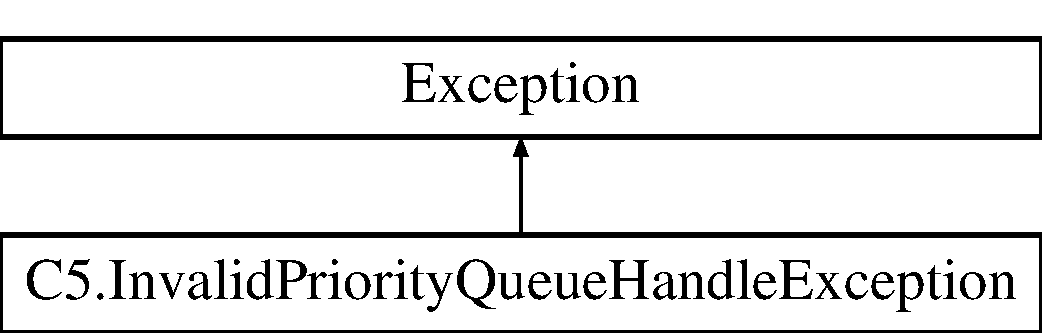
\includegraphics[height=2.000000cm]{class_c5_1_1_invalid_priority_queue_handle_exception}
\end{center}
\end{figure}
\subsection*{Public Member Functions}
\begin{DoxyCompactItemize}
\item 
\hyperlink{class_c5_1_1_invalid_priority_queue_handle_exception_a8fba5a687da5795a34fac7161c4eb2ca}{Invalid\+Priority\+Queue\+Handle\+Exception} ()
\begin{DoxyCompactList}\small\item\em Create a simple exception with no further explanation. \end{DoxyCompactList}\item 
\hyperlink{class_c5_1_1_invalid_priority_queue_handle_exception_ad771a15f55c53824ba32d0663c315c20}{Invalid\+Priority\+Queue\+Handle\+Exception} (string message)
\begin{DoxyCompactList}\small\item\em Create the exception with an explanation of the reason. \end{DoxyCompactList}\end{DoxyCompactItemize}


\subsection{Detailed Description}




\subsection{Constructor \& Destructor Documentation}
\hypertarget{class_c5_1_1_invalid_priority_queue_handle_exception_a8fba5a687da5795a34fac7161c4eb2ca}{}\index{C5\+::\+Invalid\+Priority\+Queue\+Handle\+Exception@{C5\+::\+Invalid\+Priority\+Queue\+Handle\+Exception}!Invalid\+Priority\+Queue\+Handle\+Exception@{Invalid\+Priority\+Queue\+Handle\+Exception}}
\index{Invalid\+Priority\+Queue\+Handle\+Exception@{Invalid\+Priority\+Queue\+Handle\+Exception}!C5\+::\+Invalid\+Priority\+Queue\+Handle\+Exception@{C5\+::\+Invalid\+Priority\+Queue\+Handle\+Exception}}
\subsubsection[{Invalid\+Priority\+Queue\+Handle\+Exception()}]{\setlength{\rightskip}{0pt plus 5cm}C5.\+Invalid\+Priority\+Queue\+Handle\+Exception.\+Invalid\+Priority\+Queue\+Handle\+Exception (
\begin{DoxyParamCaption}
{}
\end{DoxyParamCaption}
)}\label{class_c5_1_1_invalid_priority_queue_handle_exception_a8fba5a687da5795a34fac7161c4eb2ca}


Create a simple exception with no further explanation. 

\hypertarget{class_c5_1_1_invalid_priority_queue_handle_exception_ad771a15f55c53824ba32d0663c315c20}{}\index{C5\+::\+Invalid\+Priority\+Queue\+Handle\+Exception@{C5\+::\+Invalid\+Priority\+Queue\+Handle\+Exception}!Invalid\+Priority\+Queue\+Handle\+Exception@{Invalid\+Priority\+Queue\+Handle\+Exception}}
\index{Invalid\+Priority\+Queue\+Handle\+Exception@{Invalid\+Priority\+Queue\+Handle\+Exception}!C5\+::\+Invalid\+Priority\+Queue\+Handle\+Exception@{C5\+::\+Invalid\+Priority\+Queue\+Handle\+Exception}}
\subsubsection[{Invalid\+Priority\+Queue\+Handle\+Exception(string message)}]{\setlength{\rightskip}{0pt plus 5cm}C5.\+Invalid\+Priority\+Queue\+Handle\+Exception.\+Invalid\+Priority\+Queue\+Handle\+Exception (
\begin{DoxyParamCaption}
\item[{string}]{message}
\end{DoxyParamCaption}
)}\label{class_c5_1_1_invalid_priority_queue_handle_exception_ad771a15f55c53824ba32d0663c315c20}


Create the exception with an explanation of the reason. 


\begin{DoxyParams}{Parameters}
{\em message} & \\
\hline
\end{DoxyParams}


The documentation for this class was generated from the following file\+:\begin{DoxyCompactItemize}
\item 
C\+:/\+Users/rasmusl/\+Source/\+Repos/\+C5/\+C5/\hyperlink{_exceptions_8cs}{Exceptions.\+cs}\end{DoxyCompactItemize}

\hypertarget{interface_c5_1_1_i_persistent_sorted}{}\section{C5.\+I\+Persistent\+Sorted$<$ T $>$ Interface Template Reference}
\label{interface_c5_1_1_i_persistent_sorted}\index{C5.\+I\+Persistent\+Sorted$<$ T $>$@{C5.\+I\+Persistent\+Sorted$<$ T $>$}}


The type of a sorted collection with persistence  


Inheritance diagram for C5.\+I\+Persistent\+Sorted$<$ T $>$\+:\begin{figure}[H]
\begin{center}
\leavevmode
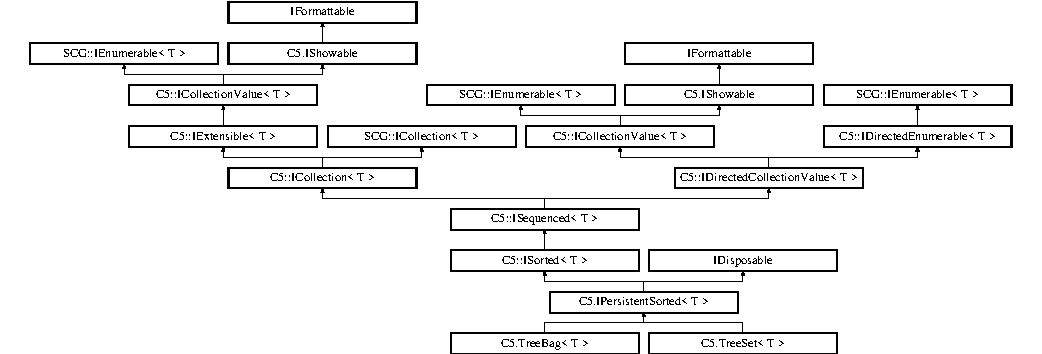
\includegraphics[height=4.732394cm]{interface_c5_1_1_i_persistent_sorted}
\end{center}
\end{figure}
\subsection*{Public Member Functions}
\begin{DoxyCompactItemize}
\item 
\hyperlink{interface_c5_1_1_i_sorted}{I\+Sorted}$<$ T $>$ \hyperlink{interface_c5_1_1_i_persistent_sorted_a9d03a4971aaffbf7c93b7aaeedca282e}{Snapshot} ()
\begin{DoxyCompactList}\small\item\em Make a (read-\/only) snap shot of this collection. \end{DoxyCompactList}\end{DoxyCompactItemize}
\subsection*{Additional Inherited Members}


\subsection{Detailed Description}
The type of a sorted collection with persistence 



\subsection{Member Function Documentation}
\hypertarget{interface_c5_1_1_i_persistent_sorted_a9d03a4971aaffbf7c93b7aaeedca282e}{}\index{C5\+::\+I\+Persistent\+Sorted@{C5\+::\+I\+Persistent\+Sorted}!Snapshot@{Snapshot}}
\index{Snapshot@{Snapshot}!C5\+::\+I\+Persistent\+Sorted@{C5\+::\+I\+Persistent\+Sorted}}
\subsubsection[{Snapshot()}]{\setlength{\rightskip}{0pt plus 5cm}{\bf I\+Sorted}$<$T$>$ {\bf C5.\+I\+Persistent\+Sorted}$<$ T $>$.Snapshot (
\begin{DoxyParamCaption}
{}
\end{DoxyParamCaption}
)}\label{interface_c5_1_1_i_persistent_sorted_a9d03a4971aaffbf7c93b7aaeedca282e}


Make a (read-\/only) snap shot of this collection. 

\begin{DoxyReturn}{Returns}
The snap shot.
\end{DoxyReturn}


Implemented in \hyperlink{class_c5_1_1_tree_bag_ad7c2d8ff62d0ffb641bf2bce4d51bd3d}{C5.\+Tree\+Bag$<$ T $>$}, and \hyperlink{class_c5_1_1_tree_set_a1ba16497dd87ddae2e4345f9b7f083e2}{C5.\+Tree\+Set$<$ T $>$}.



The documentation for this interface was generated from the following file\+:\begin{DoxyCompactItemize}
\item 
C\+:/\+Users/rasmusl/\+Source/\+Repos/\+C5/\+C5/\hyperlink{_interfaces_8cs}{Interfaces.\+cs}\end{DoxyCompactItemize}

\hypertarget{interface_c5_1_1_i_priority_queue}{}\section{C5.\+I\+Priority\+Queue$<$ T $>$ Interface Template Reference}
\label{interface_c5_1_1_i_priority_queue}\index{C5.\+I\+Priority\+Queue$<$ T $>$@{C5.\+I\+Priority\+Queue$<$ T $>$}}


A generic collection of items prioritized by a comparison (order) relation. Supports adding items and reporting or removing extremal elements.  


Inheritance diagram for C5.\+I\+Priority\+Queue$<$ T $>$\+:\begin{figure}[H]
\begin{center}
\leavevmode
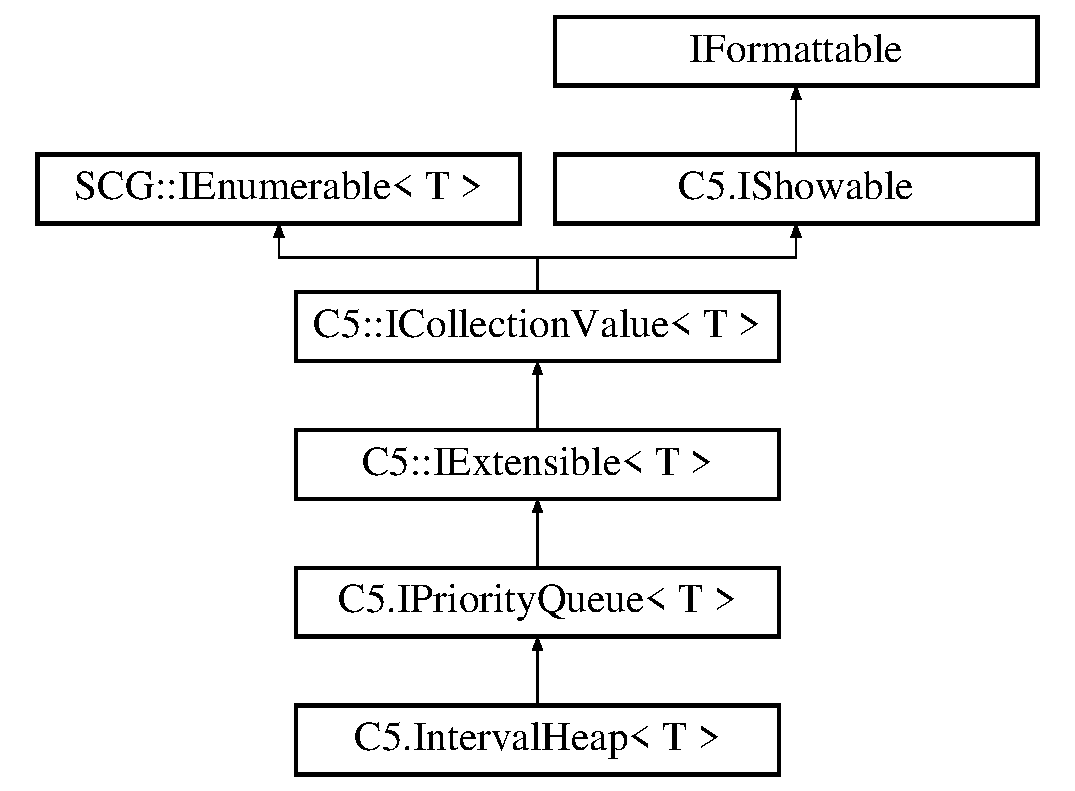
\includegraphics[height=6.000000cm]{interface_c5_1_1_i_priority_queue}
\end{center}
\end{figure}
\subsection*{Public Member Functions}
\begin{DoxyCompactItemize}
\item 
T \hyperlink{interface_c5_1_1_i_priority_queue_ac1dda27afec7f41e9b414b6e33273714}{Find\+Min} ()
\begin{DoxyCompactList}\small\item\em Find the current least item of this priority queue. \end{DoxyCompactList}\item 
T \hyperlink{interface_c5_1_1_i_priority_queue_a278dfa42e80291ba82122f174895dd77}{Delete\+Min} ()
\begin{DoxyCompactList}\small\item\em Remove the least item from this priority queue. \end{DoxyCompactList}\item 
T \hyperlink{interface_c5_1_1_i_priority_queue_ab510a95957edce0bb68aedd85abb73f8}{Find\+Max} ()
\begin{DoxyCompactList}\small\item\em Find the current largest item of this priority queue. \end{DoxyCompactList}\item 
T \hyperlink{interface_c5_1_1_i_priority_queue_a8f728da5fbc6ae1bb4b2941d51885d69}{Delete\+Max} ()
\begin{DoxyCompactList}\small\item\em Remove the largest item from this priority queue. \end{DoxyCompactList}\item 
bool \hyperlink{interface_c5_1_1_i_priority_queue_a4f8bac3647b3b668939a0e9c34c158e5}{Find} (\hyperlink{interface_c5_1_1_i_priority_queue_handle}{I\+Priority\+Queue\+Handle}$<$ T $>$ handle, out T item)
\begin{DoxyCompactList}\small\item\em Check if the entry corresponding to a handle is in the priority queue. \end{DoxyCompactList}\item 
bool \hyperlink{interface_c5_1_1_i_priority_queue_ac90f40246d54cb28935bf89d9e0c9c72}{Add} (ref \hyperlink{interface_c5_1_1_i_priority_queue_handle}{I\+Priority\+Queue\+Handle}$<$ T $>$ handle, T item)
\begin{DoxyCompactList}\small\item\em Add an item to the priority queue, receiving a handle for the item in the queue, or reusing an existing unused handle. \end{DoxyCompactList}\item 
T \hyperlink{interface_c5_1_1_i_priority_queue_a8b1272ae3287f72eeece44d17a9c2eff}{Delete} (\hyperlink{interface_c5_1_1_i_priority_queue_handle}{I\+Priority\+Queue\+Handle}$<$ T $>$ handle)
\begin{DoxyCompactList}\small\item\em Delete an item with a handle from a priority queue \end{DoxyCompactList}\item 
T \hyperlink{interface_c5_1_1_i_priority_queue_ae5784abdd5e7b6079c4cb88dd40c34ad}{Replace} (\hyperlink{interface_c5_1_1_i_priority_queue_handle}{I\+Priority\+Queue\+Handle}$<$ T $>$ handle, T item)
\begin{DoxyCompactList}\small\item\em Replace an item with a handle in a priority queue with a new item. Typically used for changing the priority of some queued object. \end{DoxyCompactList}\item 
T \hyperlink{interface_c5_1_1_i_priority_queue_af200c7e915e72ee4bf283b1bbf2eed4d}{Find\+Min} (out \hyperlink{interface_c5_1_1_i_priority_queue_handle}{I\+Priority\+Queue\+Handle}$<$ T $>$ handle)
\begin{DoxyCompactList}\small\item\em Find the current least item of this priority queue. \end{DoxyCompactList}\item 
T \hyperlink{interface_c5_1_1_i_priority_queue_afb1b1299785da3d22ac24332fafe907b}{Find\+Max} (out \hyperlink{interface_c5_1_1_i_priority_queue_handle}{I\+Priority\+Queue\+Handle}$<$ T $>$ handle)
\begin{DoxyCompactList}\small\item\em Find the current largest item of this priority queue. \end{DoxyCompactList}\item 
T \hyperlink{interface_c5_1_1_i_priority_queue_a3aca77813a8c6d30de8bc8d8ff734de0}{Delete\+Min} (out \hyperlink{interface_c5_1_1_i_priority_queue_handle}{I\+Priority\+Queue\+Handle}$<$ T $>$ handle)
\begin{DoxyCompactList}\small\item\em Remove the least item from this priority queue. \end{DoxyCompactList}\item 
T \hyperlink{interface_c5_1_1_i_priority_queue_ae6b746354d02c65d0435040682baf0c9}{Delete\+Max} (out \hyperlink{interface_c5_1_1_i_priority_queue_handle}{I\+Priority\+Queue\+Handle}$<$ T $>$ handle)
\begin{DoxyCompactList}\small\item\em Remove the largest item from this priority queue. \end{DoxyCompactList}\end{DoxyCompactItemize}
\subsection*{Properties}
\begin{DoxyCompactItemize}
\item 
S\+C\+G.\+I\+Comparer$<$ T $>$ \hyperlink{interface_c5_1_1_i_priority_queue_a23bf42fafa0689dca8f95d1ad7ee0b28}{Comparer}\hspace{0.3cm}{\ttfamily  \mbox{[}get\mbox{]}}
\begin{DoxyCompactList}\small\item\em The comparer object supplied at creation time for this collection \end{DoxyCompactList}\item 
T \hyperlink{interface_c5_1_1_i_priority_queue_a39daad6dcf3a45c1241d4d776d18bed9}{this\mbox{[}\+I\+Priority\+Queue\+Handle$<$ T $>$ handle\mbox{]}}\hspace{0.3cm}{\ttfamily  \mbox{[}get, set\mbox{]}}
\begin{DoxyCompactList}\small\item\em Get or set the item corresponding to a handle. Throws exceptions on invalid handles. \end{DoxyCompactList}\end{DoxyCompactItemize}
\subsection*{Additional Inherited Members}


\subsection{Detailed Description}
A generic collection of items prioritized by a comparison (order) relation. Supports adding items and reporting or removing extremal elements. 

When adding an item, the user may choose to have a handle allocated for this item in the queue. The resulting handle may be used for deleting the item even if not extremal, and for replacing the item. A priority queue typically only holds numeric priorities associated with some objects maintained separately in other collection objects. 

\subsection{Member Function Documentation}
\hypertarget{interface_c5_1_1_i_priority_queue_ac90f40246d54cb28935bf89d9e0c9c72}{}\index{C5\+::\+I\+Priority\+Queue@{C5\+::\+I\+Priority\+Queue}!Add@{Add}}
\index{Add@{Add}!C5\+::\+I\+Priority\+Queue@{C5\+::\+I\+Priority\+Queue}}
\subsubsection[{Add(ref I\+Priority\+Queue\+Handle$<$ T $>$ handle, T item)}]{\setlength{\rightskip}{0pt plus 5cm}bool {\bf C5.\+I\+Priority\+Queue}$<$ T $>$.Add (
\begin{DoxyParamCaption}
\item[{ref {\bf I\+Priority\+Queue\+Handle}$<$ T $>$}]{handle, }
\item[{T}]{item}
\end{DoxyParamCaption}
)}\label{interface_c5_1_1_i_priority_queue_ac90f40246d54cb28935bf89d9e0c9c72}


Add an item to the priority queue, receiving a handle for the item in the queue, or reusing an existing unused handle. 


\begin{DoxyParams}{Parameters}
{\em handle} & On output\+: a handle for the added item. On input\+: null for allocating a new handle, or a currently unused handle for reuse. A handle for reuse must be compatible with this priority queue, by being created by a priority queue of the same runtime type, but not necessarily the same priority queue object.\\
\hline
{\em item} & \\
\hline
\end{DoxyParams}
\begin{DoxyReturn}{Returns}

\end{DoxyReturn}


Implemented in \hyperlink{class_c5_1_1_interval_heap_a4ea1fbf9bb6c727fc83a033e311074ec}{C5.\+Interval\+Heap$<$ T $>$}.

\hypertarget{interface_c5_1_1_i_priority_queue_a8b1272ae3287f72eeece44d17a9c2eff}{}\index{C5\+::\+I\+Priority\+Queue@{C5\+::\+I\+Priority\+Queue}!Delete@{Delete}}
\index{Delete@{Delete}!C5\+::\+I\+Priority\+Queue@{C5\+::\+I\+Priority\+Queue}}
\subsubsection[{Delete(\+I\+Priority\+Queue\+Handle$<$ T $>$ handle)}]{\setlength{\rightskip}{0pt plus 5cm}T {\bf C5.\+I\+Priority\+Queue}$<$ T $>$.Delete (
\begin{DoxyParamCaption}
\item[{{\bf I\+Priority\+Queue\+Handle}$<$ T $>$}]{handle}
\end{DoxyParamCaption}
)}\label{interface_c5_1_1_i_priority_queue_a8b1272ae3287f72eeece44d17a9c2eff}


Delete an item with a handle from a priority queue 


\begin{DoxyParams}{Parameters}
{\em handle} & The handle for the item. The handle will be invalidated, but reusable.\\
\hline
\end{DoxyParams}
\begin{DoxyReturn}{Returns}
The deleted item
\end{DoxyReturn}


Implemented in \hyperlink{class_c5_1_1_interval_heap_a3f9868407c50d789c85e998448e50114}{C5.\+Interval\+Heap$<$ T $>$}.

\hypertarget{interface_c5_1_1_i_priority_queue_a8f728da5fbc6ae1bb4b2941d51885d69}{}\index{C5\+::\+I\+Priority\+Queue@{C5\+::\+I\+Priority\+Queue}!Delete\+Max@{Delete\+Max}}
\index{Delete\+Max@{Delete\+Max}!C5\+::\+I\+Priority\+Queue@{C5\+::\+I\+Priority\+Queue}}
\subsubsection[{Delete\+Max()}]{\setlength{\rightskip}{0pt plus 5cm}T {\bf C5.\+I\+Priority\+Queue}$<$ T $>$.Delete\+Max (
\begin{DoxyParamCaption}
{}
\end{DoxyParamCaption}
)}\label{interface_c5_1_1_i_priority_queue_a8f728da5fbc6ae1bb4b2941d51885d69}


Remove the largest item from this priority queue. 

\begin{DoxyReturn}{Returns}
The removed item.
\end{DoxyReturn}


Implemented in \hyperlink{class_c5_1_1_interval_heap_a487241b83be6837692408542c7cfb6b5}{C5.\+Interval\+Heap$<$ T $>$}.

\hypertarget{interface_c5_1_1_i_priority_queue_ae6b746354d02c65d0435040682baf0c9}{}\index{C5\+::\+I\+Priority\+Queue@{C5\+::\+I\+Priority\+Queue}!Delete\+Max@{Delete\+Max}}
\index{Delete\+Max@{Delete\+Max}!C5\+::\+I\+Priority\+Queue@{C5\+::\+I\+Priority\+Queue}}
\subsubsection[{Delete\+Max(out I\+Priority\+Queue\+Handle$<$ T $>$ handle)}]{\setlength{\rightskip}{0pt plus 5cm}T {\bf C5.\+I\+Priority\+Queue}$<$ T $>$.Delete\+Max (
\begin{DoxyParamCaption}
\item[{out {\bf I\+Priority\+Queue\+Handle}$<$ T $>$}]{handle}
\end{DoxyParamCaption}
)}\label{interface_c5_1_1_i_priority_queue_ae6b746354d02c65d0435040682baf0c9}


Remove the largest item from this priority queue. 


\begin{DoxyParams}{Parameters}
{\em handle} & On return\+: the handle of the removed item.\\
\hline
\end{DoxyParams}
\begin{DoxyReturn}{Returns}
The removed item.
\end{DoxyReturn}


Implemented in \hyperlink{class_c5_1_1_interval_heap_ac5446ec37bcee1e0f117fbbe566f6386}{C5.\+Interval\+Heap$<$ T $>$}.

\hypertarget{interface_c5_1_1_i_priority_queue_a278dfa42e80291ba82122f174895dd77}{}\index{C5\+::\+I\+Priority\+Queue@{C5\+::\+I\+Priority\+Queue}!Delete\+Min@{Delete\+Min}}
\index{Delete\+Min@{Delete\+Min}!C5\+::\+I\+Priority\+Queue@{C5\+::\+I\+Priority\+Queue}}
\subsubsection[{Delete\+Min()}]{\setlength{\rightskip}{0pt plus 5cm}T {\bf C5.\+I\+Priority\+Queue}$<$ T $>$.Delete\+Min (
\begin{DoxyParamCaption}
{}
\end{DoxyParamCaption}
)}\label{interface_c5_1_1_i_priority_queue_a278dfa42e80291ba82122f174895dd77}


Remove the least item from this priority queue. 

\begin{DoxyReturn}{Returns}
The removed item.
\end{DoxyReturn}


Implemented in \hyperlink{class_c5_1_1_interval_heap_a63772295b880e38f9ef5c2469a687770}{C5.\+Interval\+Heap$<$ T $>$}.

\hypertarget{interface_c5_1_1_i_priority_queue_a3aca77813a8c6d30de8bc8d8ff734de0}{}\index{C5\+::\+I\+Priority\+Queue@{C5\+::\+I\+Priority\+Queue}!Delete\+Min@{Delete\+Min}}
\index{Delete\+Min@{Delete\+Min}!C5\+::\+I\+Priority\+Queue@{C5\+::\+I\+Priority\+Queue}}
\subsubsection[{Delete\+Min(out I\+Priority\+Queue\+Handle$<$ T $>$ handle)}]{\setlength{\rightskip}{0pt plus 5cm}T {\bf C5.\+I\+Priority\+Queue}$<$ T $>$.Delete\+Min (
\begin{DoxyParamCaption}
\item[{out {\bf I\+Priority\+Queue\+Handle}$<$ T $>$}]{handle}
\end{DoxyParamCaption}
)}\label{interface_c5_1_1_i_priority_queue_a3aca77813a8c6d30de8bc8d8ff734de0}


Remove the least item from this priority queue. 


\begin{DoxyParams}{Parameters}
{\em handle} & On return\+: the handle of the removed item.\\
\hline
\end{DoxyParams}
\begin{DoxyReturn}{Returns}
The removed item.
\end{DoxyReturn}


Implemented in \hyperlink{class_c5_1_1_interval_heap_a3b605362b2ab7bf2268383be00015f6d}{C5.\+Interval\+Heap$<$ T $>$}.

\hypertarget{interface_c5_1_1_i_priority_queue_a4f8bac3647b3b668939a0e9c34c158e5}{}\index{C5\+::\+I\+Priority\+Queue@{C5\+::\+I\+Priority\+Queue}!Find@{Find}}
\index{Find@{Find}!C5\+::\+I\+Priority\+Queue@{C5\+::\+I\+Priority\+Queue}}
\subsubsection[{Find(\+I\+Priority\+Queue\+Handle$<$ T $>$ handle, out T item)}]{\setlength{\rightskip}{0pt plus 5cm}bool {\bf C5.\+I\+Priority\+Queue}$<$ T $>$.Find (
\begin{DoxyParamCaption}
\item[{{\bf I\+Priority\+Queue\+Handle}$<$ T $>$}]{handle, }
\item[{out T}]{item}
\end{DoxyParamCaption}
)}\label{interface_c5_1_1_i_priority_queue_a4f8bac3647b3b668939a0e9c34c158e5}


Check if the entry corresponding to a handle is in the priority queue. 


\begin{DoxyParams}{Parameters}
{\em handle} & \\
\hline
{\em item} & \\
\hline
\end{DoxyParams}
\begin{DoxyReturn}{Returns}

\end{DoxyReturn}


Implemented in \hyperlink{class_c5_1_1_interval_heap_abaae4e91221233de39a8062ae7c89402}{C5.\+Interval\+Heap$<$ T $>$}.

\hypertarget{interface_c5_1_1_i_priority_queue_ab510a95957edce0bb68aedd85abb73f8}{}\index{C5\+::\+I\+Priority\+Queue@{C5\+::\+I\+Priority\+Queue}!Find\+Max@{Find\+Max}}
\index{Find\+Max@{Find\+Max}!C5\+::\+I\+Priority\+Queue@{C5\+::\+I\+Priority\+Queue}}
\subsubsection[{Find\+Max()}]{\setlength{\rightskip}{0pt plus 5cm}T {\bf C5.\+I\+Priority\+Queue}$<$ T $>$.Find\+Max (
\begin{DoxyParamCaption}
{}
\end{DoxyParamCaption}
)}\label{interface_c5_1_1_i_priority_queue_ab510a95957edce0bb68aedd85abb73f8}


Find the current largest item of this priority queue. 

\begin{DoxyReturn}{Returns}
The largest item.
\end{DoxyReturn}


Implemented in \hyperlink{class_c5_1_1_interval_heap_abda450e3da23bc35d0db7f4f0dd91d00}{C5.\+Interval\+Heap$<$ T $>$}.

\hypertarget{interface_c5_1_1_i_priority_queue_afb1b1299785da3d22ac24332fafe907b}{}\index{C5\+::\+I\+Priority\+Queue@{C5\+::\+I\+Priority\+Queue}!Find\+Max@{Find\+Max}}
\index{Find\+Max@{Find\+Max}!C5\+::\+I\+Priority\+Queue@{C5\+::\+I\+Priority\+Queue}}
\subsubsection[{Find\+Max(out I\+Priority\+Queue\+Handle$<$ T $>$ handle)}]{\setlength{\rightskip}{0pt plus 5cm}T {\bf C5.\+I\+Priority\+Queue}$<$ T $>$.Find\+Max (
\begin{DoxyParamCaption}
\item[{out {\bf I\+Priority\+Queue\+Handle}$<$ T $>$}]{handle}
\end{DoxyParamCaption}
)}\label{interface_c5_1_1_i_priority_queue_afb1b1299785da3d22ac24332fafe907b}


Find the current largest item of this priority queue. 


\begin{DoxyParams}{Parameters}
{\em handle} & On return\+: the handle of the item.\\
\hline
\end{DoxyParams}
\begin{DoxyReturn}{Returns}
The largest item.
\end{DoxyReturn}


Implemented in \hyperlink{class_c5_1_1_interval_heap_aeb97ce7d763c7e3707251de9f76071aa}{C5.\+Interval\+Heap$<$ T $>$}.

\hypertarget{interface_c5_1_1_i_priority_queue_ac1dda27afec7f41e9b414b6e33273714}{}\index{C5\+::\+I\+Priority\+Queue@{C5\+::\+I\+Priority\+Queue}!Find\+Min@{Find\+Min}}
\index{Find\+Min@{Find\+Min}!C5\+::\+I\+Priority\+Queue@{C5\+::\+I\+Priority\+Queue}}
\subsubsection[{Find\+Min()}]{\setlength{\rightskip}{0pt plus 5cm}T {\bf C5.\+I\+Priority\+Queue}$<$ T $>$.Find\+Min (
\begin{DoxyParamCaption}
{}
\end{DoxyParamCaption}
)}\label{interface_c5_1_1_i_priority_queue_ac1dda27afec7f41e9b414b6e33273714}


Find the current least item of this priority queue. 

\begin{DoxyReturn}{Returns}
The least item.
\end{DoxyReturn}


Implemented in \hyperlink{class_c5_1_1_interval_heap_ad4671adf7daad4e8b6711c0a9a5663fe}{C5.\+Interval\+Heap$<$ T $>$}.

\hypertarget{interface_c5_1_1_i_priority_queue_af200c7e915e72ee4bf283b1bbf2eed4d}{}\index{C5\+::\+I\+Priority\+Queue@{C5\+::\+I\+Priority\+Queue}!Find\+Min@{Find\+Min}}
\index{Find\+Min@{Find\+Min}!C5\+::\+I\+Priority\+Queue@{C5\+::\+I\+Priority\+Queue}}
\subsubsection[{Find\+Min(out I\+Priority\+Queue\+Handle$<$ T $>$ handle)}]{\setlength{\rightskip}{0pt plus 5cm}T {\bf C5.\+I\+Priority\+Queue}$<$ T $>$.Find\+Min (
\begin{DoxyParamCaption}
\item[{out {\bf I\+Priority\+Queue\+Handle}$<$ T $>$}]{handle}
\end{DoxyParamCaption}
)}\label{interface_c5_1_1_i_priority_queue_af200c7e915e72ee4bf283b1bbf2eed4d}


Find the current least item of this priority queue. 


\begin{DoxyParams}{Parameters}
{\em handle} & On return\+: the handle of the item.\\
\hline
\end{DoxyParams}
\begin{DoxyReturn}{Returns}
The least item.
\end{DoxyReturn}


Implemented in \hyperlink{class_c5_1_1_interval_heap_a3b14d4af51572b295c9eebdf880ed493}{C5.\+Interval\+Heap$<$ T $>$}.

\hypertarget{interface_c5_1_1_i_priority_queue_ae5784abdd5e7b6079c4cb88dd40c34ad}{}\index{C5\+::\+I\+Priority\+Queue@{C5\+::\+I\+Priority\+Queue}!Replace@{Replace}}
\index{Replace@{Replace}!C5\+::\+I\+Priority\+Queue@{C5\+::\+I\+Priority\+Queue}}
\subsubsection[{Replace(\+I\+Priority\+Queue\+Handle$<$ T $>$ handle, T item)}]{\setlength{\rightskip}{0pt plus 5cm}T {\bf C5.\+I\+Priority\+Queue}$<$ T $>$.Replace (
\begin{DoxyParamCaption}
\item[{{\bf I\+Priority\+Queue\+Handle}$<$ T $>$}]{handle, }
\item[{T}]{item}
\end{DoxyParamCaption}
)}\label{interface_c5_1_1_i_priority_queue_ae5784abdd5e7b6079c4cb88dd40c34ad}


Replace an item with a handle in a priority queue with a new item. Typically used for changing the priority of some queued object. 


\begin{DoxyParams}{Parameters}
{\em handle} & The handle for the old item\\
\hline
{\em item} & The new item\\
\hline
\end{DoxyParams}
\begin{DoxyReturn}{Returns}
The old item
\end{DoxyReturn}


Implemented in \hyperlink{class_c5_1_1_interval_heap_abfc2e592410f83b10f7feb82bcbd53db}{C5.\+Interval\+Heap$<$ T $>$}.



\subsection{Property Documentation}
\hypertarget{interface_c5_1_1_i_priority_queue_a23bf42fafa0689dca8f95d1ad7ee0b28}{}\index{C5\+::\+I\+Priority\+Queue@{C5\+::\+I\+Priority\+Queue}!Comparer@{Comparer}}
\index{Comparer@{Comparer}!C5\+::\+I\+Priority\+Queue@{C5\+::\+I\+Priority\+Queue}}
\subsubsection[{Comparer}]{\setlength{\rightskip}{0pt plus 5cm}S\+C\+G.\+I\+Comparer$<$T$>$ {\bf C5.\+I\+Priority\+Queue}$<$ T $>$.Comparer\hspace{0.3cm}{\ttfamily [get]}}\label{interface_c5_1_1_i_priority_queue_a23bf42fafa0689dca8f95d1ad7ee0b28}


The comparer object supplied at creation time for this collection 

The comparer\hypertarget{interface_c5_1_1_i_priority_queue_a39daad6dcf3a45c1241d4d776d18bed9}{}\index{C5\+::\+I\+Priority\+Queue@{C5\+::\+I\+Priority\+Queue}!this\mbox{[}\+I\+Priority\+Queue\+Handle$<$ T $>$ handle\mbox{]}@{this[I\+Priority\+Queue\+Handle$<$ T $>$ handle]}}
\index{this\mbox{[}\+I\+Priority\+Queue\+Handle$<$ T $>$ handle\mbox{]}@{this[I\+Priority\+Queue\+Handle$<$ T $>$ handle]}!C5\+::\+I\+Priority\+Queue@{C5\+::\+I\+Priority\+Queue}}
\subsubsection[{this[I\+Priority\+Queue\+Handle$<$ T $>$ handle]}]{\setlength{\rightskip}{0pt plus 5cm}T {\bf C5.\+I\+Priority\+Queue}$<$ T $>$.this\mbox{[}{\bf I\+Priority\+Queue\+Handle}$<$ T $>$ handle\mbox{]}\hspace{0.3cm}{\ttfamily [get]}, {\ttfamily [set]}}\label{interface_c5_1_1_i_priority_queue_a39daad6dcf3a45c1241d4d776d18bed9}


Get or set the item corresponding to a handle. Throws exceptions on invalid handles. 


\begin{DoxyParams}{Parameters}
{\em handle} & \\
\hline
\end{DoxyParams}
\begin{DoxyReturn}{Returns}

\end{DoxyReturn}


The documentation for this interface was generated from the following file\+:\begin{DoxyCompactItemize}
\item 
C\+:/\+Users/rasmusl/\+Source/\+Repos/\+C5/\+C5/\hyperlink{_interfaces_8cs}{Interfaces.\+cs}\end{DoxyCompactItemize}

\hypertarget{interface_c5_1_1_i_priority_queue_handle}{}\section{C5.\+I\+Priority\+Queue\+Handle$<$ T $>$ Interface Template Reference}
\label{interface_c5_1_1_i_priority_queue_handle}\index{C5.\+I\+Priority\+Queue\+Handle$<$ T $>$@{C5.\+I\+Priority\+Queue\+Handle$<$ T $>$}}


The base type of a priority queue handle  




\subsection{Detailed Description}
The base type of a priority queue handle 


\begin{DoxyTemplParams}{Template Parameters}
{\em T} & \\
\hline
\end{DoxyTemplParams}


The documentation for this interface was generated from the following file\+:\begin{DoxyCompactItemize}
\item 
C\+:/\+Users/rasmusl/\+Source/\+Repos/\+C5/\+C5/\hyperlink{_interfaces_8cs}{Interfaces.\+cs}\end{DoxyCompactItemize}

\hypertarget{interface_c5_1_1_i_queue}{}\section{C5.\+I\+Queue$<$ T $>$ Interface Template Reference}
\label{interface_c5_1_1_i_queue}\index{C5.\+I\+Queue$<$ T $>$@{C5.\+I\+Queue$<$ T $>$}}


The interface describing the operations of a F\+I\+F\+O queue data structure.  


Inheritance diagram for C5.\+I\+Queue$<$ T $>$\+:\begin{figure}[H]
\begin{center}
\leavevmode
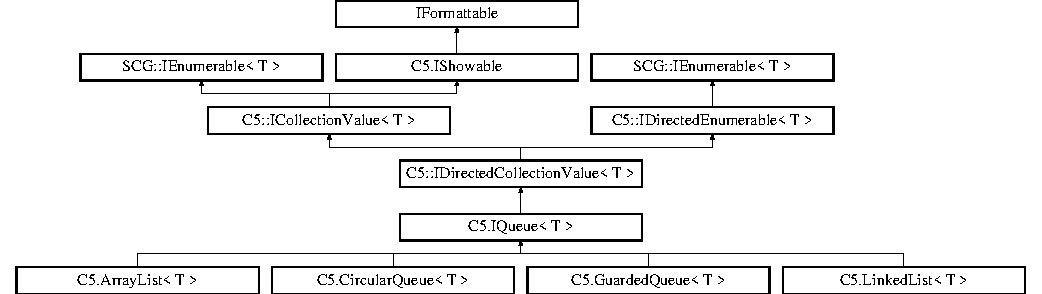
\includegraphics[height=3.943662cm]{interface_c5_1_1_i_queue}
\end{center}
\end{figure}
\subsection*{Public Member Functions}
\begin{DoxyCompactItemize}
\item 
void \hyperlink{interface_c5_1_1_i_queue_afceb820ca32b996f6fd5c34a85ccbacd}{Enqueue} (T item)
\begin{DoxyCompactList}\small\item\em Enqueue an item at the back of the queue. \end{DoxyCompactList}\item 
T \hyperlink{interface_c5_1_1_i_queue_ae64bb24d3237ad9cef4f55593ca20bc7}{Dequeue} ()
\begin{DoxyCompactList}\small\item\em Dequeue an item from the front of the queue. \end{DoxyCompactList}\end{DoxyCompactItemize}
\subsection*{Properties}
\begin{DoxyCompactItemize}
\item 
bool \hyperlink{interface_c5_1_1_i_queue_ab3c0251c21b3054813279abb3377d4f8}{Allows\+Duplicates}\hspace{0.3cm}{\ttfamily  \mbox{[}get\mbox{]}}
\item 
T \hyperlink{interface_c5_1_1_i_queue_a750c0af1f1ec226a1729f841fcc1dfe9}{this\mbox{[}int index\mbox{]}}\hspace{0.3cm}{\ttfamily  \mbox{[}get\mbox{]}}
\begin{DoxyCompactList}\small\item\em Get the \end{DoxyCompactList}\end{DoxyCompactItemize}
\subsection*{Additional Inherited Members}


\subsection{Detailed Description}
The interface describing the operations of a F\+I\+F\+O queue data structure. 


\begin{DoxyTemplParams}{Template Parameters}
{\em T} & The item type\\
\hline
\end{DoxyTemplParams}


\subsection{Member Function Documentation}
\hypertarget{interface_c5_1_1_i_queue_ae64bb24d3237ad9cef4f55593ca20bc7}{}\index{C5\+::\+I\+Queue@{C5\+::\+I\+Queue}!Dequeue@{Dequeue}}
\index{Dequeue@{Dequeue}!C5\+::\+I\+Queue@{C5\+::\+I\+Queue}}
\subsubsection[{Dequeue()}]{\setlength{\rightskip}{0pt plus 5cm}T {\bf C5.\+I\+Queue}$<$ T $>$.Dequeue (
\begin{DoxyParamCaption}
{}
\end{DoxyParamCaption}
)}\label{interface_c5_1_1_i_queue_ae64bb24d3237ad9cef4f55593ca20bc7}


Dequeue an item from the front of the queue. 

\begin{DoxyReturn}{Returns}
The item
\end{DoxyReturn}


Implemented in \hyperlink{class_c5_1_1_linked_list_a5175726bb9e1356d3442b427acac06b5}{C5.\+Linked\+List$<$ T $>$}, \hyperlink{class_c5_1_1_array_list_a82a4b5a21129d4cffe69fa53b9bfe827}{C5.\+Array\+List$<$ T $>$}, \hyperlink{class_c5_1_1_guarded_queue_aeac8a6ef430740f2ec1df8346cd122a4}{C5.\+Guarded\+Queue$<$ T $>$}, and \hyperlink{class_c5_1_1_circular_queue_ad52b370d4ab23656feeeeddf840da857}{C5.\+Circular\+Queue$<$ T $>$}.

\hypertarget{interface_c5_1_1_i_queue_afceb820ca32b996f6fd5c34a85ccbacd}{}\index{C5\+::\+I\+Queue@{C5\+::\+I\+Queue}!Enqueue@{Enqueue}}
\index{Enqueue@{Enqueue}!C5\+::\+I\+Queue@{C5\+::\+I\+Queue}}
\subsubsection[{Enqueue(\+T item)}]{\setlength{\rightskip}{0pt plus 5cm}void {\bf C5.\+I\+Queue}$<$ T $>$.Enqueue (
\begin{DoxyParamCaption}
\item[{T}]{item}
\end{DoxyParamCaption}
)}\label{interface_c5_1_1_i_queue_afceb820ca32b996f6fd5c34a85ccbacd}


Enqueue an item at the back of the queue. 


\begin{DoxyParams}{Parameters}
{\em item} & The item\\
\hline
\end{DoxyParams}


Implemented in \hyperlink{class_c5_1_1_linked_list_af48722fbdb04653c4dc7f6bf8af7562c}{C5.\+Linked\+List$<$ T $>$}, \hyperlink{class_c5_1_1_array_list_ac19b1fa4c34de8cf94afa85b325c5646}{C5.\+Array\+List$<$ T $>$}, \hyperlink{class_c5_1_1_guarded_queue_af8b4a6e503df67d019015f2ccce7c06b}{C5.\+Guarded\+Queue$<$ T $>$}, and \hyperlink{class_c5_1_1_circular_queue_a38228eb467c6366bbdfe930af2a6a3f7}{C5.\+Circular\+Queue$<$ T $>$}.



\subsection{Property Documentation}
\hypertarget{interface_c5_1_1_i_queue_ab3c0251c21b3054813279abb3377d4f8}{}\index{C5\+::\+I\+Queue@{C5\+::\+I\+Queue}!Allows\+Duplicates@{Allows\+Duplicates}}
\index{Allows\+Duplicates@{Allows\+Duplicates}!C5\+::\+I\+Queue@{C5\+::\+I\+Queue}}
\subsubsection[{Allows\+Duplicates}]{\setlength{\rightskip}{0pt plus 5cm}bool {\bf C5.\+I\+Queue}$<$ T $>$.Allows\+Duplicates\hspace{0.3cm}{\ttfamily [get]}}\label{interface_c5_1_1_i_queue_ab3c0251c21b3054813279abb3377d4f8}




\hypertarget{interface_c5_1_1_i_queue_a750c0af1f1ec226a1729f841fcc1dfe9}{}\index{C5\+::\+I\+Queue@{C5\+::\+I\+Queue}!this\mbox{[}int index\mbox{]}@{this[int index]}}
\index{this\mbox{[}int index\mbox{]}@{this[int index]}!C5\+::\+I\+Queue@{C5\+::\+I\+Queue}}
\subsubsection[{this[int index]}]{\setlength{\rightskip}{0pt plus 5cm}T {\bf C5.\+I\+Queue}$<$ T $>$.this\mbox{[}int index\mbox{]}\hspace{0.3cm}{\ttfamily [get]}}\label{interface_c5_1_1_i_queue_a750c0af1f1ec226a1729f841fcc1dfe9}


Get the 

{\ttfamily index}\textquotesingle{}th element of the queue. The front of the queue has index 0. 


\begin{DoxyParams}{Parameters}
{\em index} & \\
\hline
\end{DoxyParams}
\begin{DoxyReturn}{Returns}

\end{DoxyReturn}


The documentation for this interface was generated from the following file\+:\begin{DoxyCompactItemize}
\item 
C\+:/\+Users/rasmusl/\+Source/\+Repos/\+C5/\+C5/\hyperlink{_interfaces_8cs}{Interfaces.\+cs}\end{DoxyCompactItemize}

\hypertarget{interface_c5_1_1_i_sequenced}{}\section{C5.\+I\+Sequenced$<$ T $>$ Interface Template Reference}
\label{interface_c5_1_1_i_sequenced}\index{C5.\+I\+Sequenced$<$ T $>$@{C5.\+I\+Sequenced$<$ T $>$}}


An editable collection maintaining a definite sequence order of the items.  


Inheritance diagram for C5.\+I\+Sequenced$<$ T $>$\+:\begin{figure}[H]
\begin{center}
\leavevmode
\includegraphics[height=3.346138cm]{interface_c5_1_1_i_sequenced}
\end{center}
\end{figure}
\subsection*{Public Member Functions}
\begin{DoxyCompactItemize}
\item 
int \hyperlink{interface_c5_1_1_i_sequenced_afb06eeccff646bb763c76c1826b177fe}{Get\+Sequenced\+Hash\+Code} ()
\begin{DoxyCompactList}\small\item\em The hashcode is defined as \end{DoxyCompactList}\item 
bool \hyperlink{interface_c5_1_1_i_sequenced_aeb2be77c5c30ab10f468222f6cbb795f}{Sequenced\+Equals} (\hyperlink{interface_c5_1_1_i_sequenced}{I\+Sequenced}$<$ T $>$ other\+Collection)
\begin{DoxyCompactList}\small\item\em Compare this sequenced collection to another one in sequence order. \end{DoxyCompactList}\end{DoxyCompactItemize}
\subsection*{Additional Inherited Members}


\subsection{Detailed Description}
An editable collection maintaining a definite sequence order of the items. 

{\itshape Implementations of this interface must compute the hash code and equality exactly as prescribed in the method definitions in order to be consistent with other collection classes implementing this interface.} {\itshape This interface is usually implemented by explicit interface implementation, not as ordinary virtual methods.} 

\subsection{Member Function Documentation}
\hypertarget{interface_c5_1_1_i_sequenced_afb06eeccff646bb763c76c1826b177fe}{}\index{C5\+::\+I\+Sequenced@{C5\+::\+I\+Sequenced}!Get\+Sequenced\+Hash\+Code@{Get\+Sequenced\+Hash\+Code}}
\index{Get\+Sequenced\+Hash\+Code@{Get\+Sequenced\+Hash\+Code}!C5\+::\+I\+Sequenced@{C5\+::\+I\+Sequenced}}
\subsubsection[{Get\+Sequenced\+Hash\+Code()}]{\setlength{\rightskip}{0pt plus 5cm}int {\bf C5.\+I\+Sequenced}$<$ T $>$.Get\+Sequenced\+Hash\+Code (
\begin{DoxyParamCaption}
{}
\end{DoxyParamCaption}
)}\label{interface_c5_1_1_i_sequenced_afb06eeccff646bb763c76c1826b177fe}


The hashcode is defined as 

{\ttfamily h(...h(h(h(x1),x2),x3),...,xn)} for {\ttfamily h(a,b)=C\+O\+N\+S\+T\+A\+N\+T$\ast$a+b} and the x\textquotesingle{}s the hash codes of the items of this collection. 

\begin{DoxyReturn}{Returns}
The sequence order hashcode of this collection.
\end{DoxyReturn}


Implemented in \hyperlink{class_c5_1_1_hashed_linked_list_ab1ef52935e3a9a7ba78b1ddecc7a696e}{C5.\+Hashed\+Linked\+List$<$ T $>$}, \hyperlink{class_c5_1_1_linked_list_a8318b5b0ea81fb23e601e8321699851a}{C5.\+Linked\+List$<$ T $>$}, \hyperlink{class_c5_1_1_guarded_sequenced_a04214406cd7fe4814643b79c5005c799}{C5.\+Guarded\+Sequenced$<$ T $>$}, and \hyperlink{class_c5_1_1_wrapped_array_a00b82e37ca65bf9ea9088f5528b07fc4}{C5.\+Wrapped\+Array$<$ T $>$}.

\hypertarget{interface_c5_1_1_i_sequenced_aeb2be77c5c30ab10f468222f6cbb795f}{}\index{C5\+::\+I\+Sequenced@{C5\+::\+I\+Sequenced}!Sequenced\+Equals@{Sequenced\+Equals}}
\index{Sequenced\+Equals@{Sequenced\+Equals}!C5\+::\+I\+Sequenced@{C5\+::\+I\+Sequenced}}
\subsubsection[{Sequenced\+Equals(\+I\+Sequenced$<$ T $>$ other\+Collection)}]{\setlength{\rightskip}{0pt plus 5cm}bool {\bf C5.\+I\+Sequenced}$<$ T $>$.Sequenced\+Equals (
\begin{DoxyParamCaption}
\item[{{\bf I\+Sequenced}$<$ T $>$}]{other\+Collection}
\end{DoxyParamCaption}
)}\label{interface_c5_1_1_i_sequenced_aeb2be77c5c30ab10f468222f6cbb795f}


Compare this sequenced collection to another one in sequence order. 


\begin{DoxyParams}{Parameters}
{\em other\+Collection} & The sequenced collection to compare to.\\
\hline
\end{DoxyParams}
\begin{DoxyReturn}{Returns}
True if this collection and that contains equal (according to this collection\textquotesingle{}s itemequality\+Comparer) in the same sequence order.
\end{DoxyReturn}


Implemented in \hyperlink{class_c5_1_1_hashed_linked_list_a473d18abd8b89ee61184fd6731e76029}{C5.\+Hashed\+Linked\+List$<$ T $>$}, \hyperlink{class_c5_1_1_linked_list_a3d2f19d9264bfc3076be39c03429a7aa}{C5.\+Linked\+List$<$ T $>$}, \hyperlink{class_c5_1_1_guarded_sequenced_ac4377e7ad77d3954865ad6500fb47245}{C5.\+Guarded\+Sequenced$<$ T $>$}, and \hyperlink{class_c5_1_1_wrapped_array_a3a74f3b059b10576670618716cc3377f}{C5.\+Wrapped\+Array$<$ T $>$}.



The documentation for this interface was generated from the following file\+:\begin{DoxyCompactItemize}
\item 
C\+:/\+Users/rasmusl/\+Source/\+Repos/\+C5/\+C5/\hyperlink{_interfaces_8cs}{Interfaces.\+cs}\end{DoxyCompactItemize}

\hypertarget{interface_c5_1_1_i_showable}{}\section{C5.\+I\+Showable Interface Reference}
\label{interface_c5_1_1_i_showable}\index{C5.\+I\+Showable@{C5.\+I\+Showable}}


{\itshape (Describe usage of \char`\"{}\+L\+:300\char`\"{} format string.)}  


Inheritance diagram for C5.\+I\+Showable\+:\begin{figure}[H]
\begin{center}
\leavevmode
\includegraphics[height=2.178988cm]{interface_c5_1_1_i_showable}
\end{center}
\end{figure}
\subsection*{Public Member Functions}
\begin{DoxyCompactItemize}
\item 
bool \hyperlink{interface_c5_1_1_i_showable_a0605b632e204023f0b32b2aec8e6ad27}{Show} (String\+Builder stringbuilder, ref int rest, I\+Format\+Provider format\+Provider)
\begin{DoxyCompactList}\small\item\em Format \end{DoxyCompactList}\end{DoxyCompactItemize}


\subsection{Detailed Description}
{\itshape (Describe usage of \char`\"{}\+L\+:300\char`\"{} format string.)} 



\subsection{Member Function Documentation}
\hypertarget{interface_c5_1_1_i_showable_a0605b632e204023f0b32b2aec8e6ad27}{}\index{C5\+::\+I\+Showable@{C5\+::\+I\+Showable}!Show@{Show}}
\index{Show@{Show}!C5\+::\+I\+Showable@{C5\+::\+I\+Showable}}
\subsubsection[{Show(\+String\+Builder stringbuilder, ref int rest, I\+Format\+Provider format\+Provider)}]{\setlength{\rightskip}{0pt plus 5cm}bool C5.\+I\+Showable.\+Show (
\begin{DoxyParamCaption}
\item[{String\+Builder}]{stringbuilder, }
\item[{ref int}]{rest, }
\item[{I\+Format\+Provider}]{format\+Provider}
\end{DoxyParamCaption}
)}\label{interface_c5_1_1_i_showable_a0605b632e204023f0b32b2aec8e6ad27}


Format 

{\ttfamily this} using at most approximately {\ttfamily rest} chars and append the result, possibly truncated, to stringbuilder. Subtract the actual number of used chars from {\ttfamily rest}. 


\begin{DoxyParams}{Parameters}
{\em stringbuilder} & \\
\hline
{\em rest} & \\
\hline
{\em format\+Provider} & \\
\hline
\end{DoxyParams}
\begin{DoxyReturn}{Returns}
True if the appended formatted string was complete (not truncated).
\end{DoxyReturn}


Implemented in \hyperlink{class_c5_1_1_wrapped_array_a434aab84ad13ca5702baada927f6fcdf}{C5.\+Wrapped\+Array$<$ T $>$}.



The documentation for this interface was generated from the following file\+:\begin{DoxyCompactItemize}
\item 
C\+:/\+Users/rasmusl/\+Source/\+Repos/\+C5/\+C5/\hyperlink{_formatting_8cs}{Formatting.\+cs}\end{DoxyCompactItemize}

\hypertarget{interface_c5_1_1_i_sorted}{}\section{C5.\+I\+Sorted$<$ T $>$ Interface Template Reference}
\label{interface_c5_1_1_i_sorted}\index{C5.\+I\+Sorted$<$ T $>$@{C5.\+I\+Sorted$<$ T $>$}}


A sorted collection, i.\+e. a collection where items are maintained and can be searched for in sorted order. Thus the sequence order is given as a sorting order.  


Inheritance diagram for C5.\+I\+Sorted$<$ T $>$\+:\begin{figure}[H]
\begin{center}
\leavevmode
\includegraphics[height=3.380281cm]{interface_c5_1_1_i_sorted}
\end{center}
\end{figure}
\subsection*{Public Member Functions}
\begin{DoxyCompactItemize}
\item 
T \hyperlink{interface_c5_1_1_i_sorted_ad7a7fc9df9ff4fd5e5ab399c5703f995}{Find\+Min} ()
\begin{DoxyCompactList}\small\item\em Find the current least item of this sorted collection. \end{DoxyCompactList}\item 
T \hyperlink{interface_c5_1_1_i_sorted_ad30bc55d0c81e695896d459422b76954}{Delete\+Min} ()
\begin{DoxyCompactList}\small\item\em Remove the least item from this sorted collection. \end{DoxyCompactList}\item 
T \hyperlink{interface_c5_1_1_i_sorted_a9321a921a443cfd8411534fbef19ab00}{Find\+Max} ()
\begin{DoxyCompactList}\small\item\em Find the current largest item of this sorted collection. \end{DoxyCompactList}\item 
T \hyperlink{interface_c5_1_1_i_sorted_a58b26b758745ad2146252b9e5ff2965b}{Delete\+Max} ()
\begin{DoxyCompactList}\small\item\em Remove the largest item from this sorted collection. \end{DoxyCompactList}\item 
bool \hyperlink{interface_c5_1_1_i_sorted_ad8189cb7e5d50d33a24a75641eaeab34}{Try\+Predecessor} (T item, out T res)
\begin{DoxyCompactList}\small\item\em Find the strict predecessor of item in the sorted collection, that is, the greatest item in the collection smaller than the item. \end{DoxyCompactList}\item 
bool \hyperlink{interface_c5_1_1_i_sorted_a578a0b4db8e2b04543c72d1bf645ce65}{Try\+Successor} (T item, out T res)
\begin{DoxyCompactList}\small\item\em Find the strict successor of item in the sorted collection, that is, the least item in the collection greater than the supplied value. \end{DoxyCompactList}\item 
bool \hyperlink{interface_c5_1_1_i_sorted_aeabd71eb284ab4130d190b60a2f64584}{Try\+Weak\+Predecessor} (T item, out T res)
\begin{DoxyCompactList}\small\item\em Find the weak predecessor of item in the sorted collection, that is, the greatest item in the collection smaller than or equal to the item. \end{DoxyCompactList}\item 
bool \hyperlink{interface_c5_1_1_i_sorted_ace630ae0bea6fd7772e6e9fa21ea2567}{Try\+Weak\+Successor} (T item, out T res)
\begin{DoxyCompactList}\small\item\em Find the weak successor of item in the sorted collection, that is, the least item in the collection greater than or equal to the supplied value. \end{DoxyCompactList}\item 
T \hyperlink{interface_c5_1_1_i_sorted_a973bf071df358a008bdfed289a38ff71}{Predecessor} (T item)
\begin{DoxyCompactList}\small\item\em Find the strict predecessor in the sorted collection of a particular value, that is, the largest item in the collection less than the supplied value. \end{DoxyCompactList}\item 
T \hyperlink{interface_c5_1_1_i_sorted_a6620b9769f5125157e254d8077744515}{Successor} (T item)
\begin{DoxyCompactList}\small\item\em Find the strict successor in the sorted collection of a particular value, that is, the least item in the collection greater than the supplied value. \end{DoxyCompactList}\item 
T \hyperlink{interface_c5_1_1_i_sorted_aac28eacc400148e84e0d24e14709a9f7}{Weak\+Predecessor} (T item)
\begin{DoxyCompactList}\small\item\em Find the weak predecessor in the sorted collection of a particular value, that is, the largest item in the collection less than or equal to the supplied value. \end{DoxyCompactList}\item 
T \hyperlink{interface_c5_1_1_i_sorted_a52c5bf3983dfb2378ec431206d1ee8ce}{Weak\+Successor} (T item)
\begin{DoxyCompactList}\small\item\em Find the weak successor in the sorted collection of a particular value, that is, the least item in the collection greater than or equal to the supplied value. \end{DoxyCompactList}\item 
bool \hyperlink{interface_c5_1_1_i_sorted_a7acdf0ef5765c2554e5efa8df856c2b4}{Cut} (I\+Comparable$<$ T $>$ cut\+Function, out T low, out bool low\+Is\+Valid, out T high, out bool high\+Is\+Valid)
\begin{DoxyCompactList}\small\item\em Given a \char`\"{}cut\char`\"{} function from the items of the sorted collection to \end{DoxyCompactList}\item 
\hyperlink{interface_c5_1_1_i_directed_enumerable}{I\+Directed\+Enumerable}$<$ T $>$ \hyperlink{interface_c5_1_1_i_sorted_a0eabf2b7418467cf0ee1cfb15b6b9e34}{Range\+From} (T bot)
\begin{DoxyCompactList}\small\item\em Query this sorted collection for items greater than or equal to a supplied value. \end{DoxyCompactList}\item 
\hyperlink{interface_c5_1_1_i_directed_enumerable}{I\+Directed\+Enumerable}$<$ T $>$ \hyperlink{interface_c5_1_1_i_sorted_a66a3e2a57ca820b3a67b2f8d99e3c7cb}{Range\+From\+To} (T bot, T top)
\begin{DoxyCompactList}\small\item\em Query this sorted collection for items between two supplied values. \end{DoxyCompactList}\item 
\hyperlink{interface_c5_1_1_i_directed_enumerable}{I\+Directed\+Enumerable}$<$ T $>$ \hyperlink{interface_c5_1_1_i_sorted_a438ee04db17957587e7651f4c010814a}{Range\+To} (T top)
\begin{DoxyCompactList}\small\item\em Query this sorted collection for items less than a supplied value. \end{DoxyCompactList}\item 
\hyperlink{interface_c5_1_1_i_directed_collection_value}{I\+Directed\+Collection\+Value}$<$ T $>$ \hyperlink{interface_c5_1_1_i_sorted_ad90021b06a8976cc8c043104cf8e1ca4}{Range\+All} ()
\begin{DoxyCompactList}\small\item\em Create a directed collection with the same items as this collection. \end{DoxyCompactList}\item 
void \hyperlink{interface_c5_1_1_i_sorted_a51dd21143c9438dc9f841a9d7b6f6b3f}{Add\+Sorted} (S\+C\+G.\+I\+Enumerable$<$ T $>$ items)
\begin{DoxyCompactList}\small\item\em Add all the items from another collection with an enumeration order that is increasing in the items. \end{DoxyCompactList}\item 
void \hyperlink{interface_c5_1_1_i_sorted_ab6f6647d63da58ce3b6d837fd73ff0a1}{Remove\+Range\+From} (T low)
\begin{DoxyCompactList}\small\item\em Remove all items of this collection above or at a supplied threshold. \end{DoxyCompactList}\item 
void \hyperlink{interface_c5_1_1_i_sorted_a3d2125d5a4b4c5ce0fb34fcb8be0fa72}{Remove\+Range\+From\+To} (T low, T hi)
\begin{DoxyCompactList}\small\item\em Remove all items of this collection between two supplied thresholds. \end{DoxyCompactList}\item 
void \hyperlink{interface_c5_1_1_i_sorted_ad2e5ddc9c56ecf42340571bdfabf5d22}{Remove\+Range\+To} (T hi)
\begin{DoxyCompactList}\small\item\em Remove all items of this collection below a supplied threshold. \end{DoxyCompactList}\end{DoxyCompactItemize}
\subsection*{Properties}
\begin{DoxyCompactItemize}
\item 
S\+C\+G.\+I\+Comparer$<$ T $>$ \hyperlink{interface_c5_1_1_i_sorted_a8daa86df3d094c47142596d1c102726c}{Comparer}\hspace{0.3cm}{\ttfamily  \mbox{[}get\mbox{]}}
\begin{DoxyCompactList}\small\item\em The comparer object supplied at creation time for this sorted collection. \end{DoxyCompactList}\end{DoxyCompactItemize}
\subsection*{Additional Inherited Members}


\subsection{Detailed Description}
A sorted collection, i.\+e. a collection where items are maintained and can be searched for in sorted order. Thus the sequence order is given as a sorting order. 

The sorting order is defined by a comparer, an object of type I\+Comparer$<$T$>$ (T\+:\+C5.\+I\+Comparer`1). Implementors of this interface will normally let the user define the comparer as an argument to a constructor. Usually there will also be constructors without a comparer argument, in which case the comparer should be the defalt comparer for the item type, P\+:\+C5.\+Comparer`1.\+Default.

The comparer of the sorted collection is available as the {\ttfamily S\+C\+G.\+Comparer} property (P\+:\+C5.\+I\+Sorted`1.\+Comparer).

The methods are grouped according to 
\begin{DoxyItemize}
\item Extrema\+: report or report and delete an extremal item. This is reminiscent of simplified priority queues. 
\item Nearest neighbor\+: report predecessor or successor in the collection of an item. Cut belongs to this group. 
\item Range\+: report a view of a range of elements or remove all elements in a range. 
\item Add\+Sorted\+: add a collection of items known to be sorted in the same order (should be faster) (to be removed?) 
\end{DoxyItemize}

Since this interface extends \hyperlink{interface_c5_1_1_i_sequenced}{I\+Sequenced}$<$T$>$, sorted collections will also have an item equality\+Comparer (P\+:\+C5.\+I\+Extensible`1.\+Equality\+Comparer). This equality\+Comparer will not be used in connection with the inner workings of the sorted collection, but will be used if the sorted collection is used as an item in a collection of unsequenced or sequenced collections, (T\+:\+C5.\+I\+Collection`1 and T\+:\+C5.\+I\+Sequenced`1)

Note that code may check if two sorted collections has the same sorting order by checking if the Comparer properties are equal. This is done a few places in this library for optimization purposes.

\subsection{Member Function Documentation}
\hypertarget{interface_c5_1_1_i_sorted_a51dd21143c9438dc9f841a9d7b6f6b3f}{}\index{C5\+::\+I\+Sorted@{C5\+::\+I\+Sorted}!Add\+Sorted@{Add\+Sorted}}
\index{Add\+Sorted@{Add\+Sorted}!C5\+::\+I\+Sorted@{C5\+::\+I\+Sorted}}
\subsubsection[{Add\+Sorted(\+S\+C\+G.\+I\+Enumerable$<$ T $>$ items)}]{\setlength{\rightskip}{0pt plus 5cm}void {\bf C5.\+I\+Sorted}$<$ T $>$.Add\+Sorted (
\begin{DoxyParamCaption}
\item[{S\+C\+G.\+I\+Enumerable$<$ T $>$}]{items}
\end{DoxyParamCaption}
)}\label{interface_c5_1_1_i_sorted_a51dd21143c9438dc9f841a9d7b6f6b3f}


Add all the items from another collection with an enumeration order that is increasing in the items. 


\begin{DoxyExceptions}{Exceptions}
{\em Argument\+Exception} & if the enumerated items turns out not to be in increasing order.\\
\hline
\end{DoxyExceptions}

\begin{DoxyParams}{Parameters}
{\em items} & The collection to add.\\
\hline
\end{DoxyParams}


Implemented in \hyperlink{class_c5_1_1_guarded_sorted_a5dfe71d83337e50a8d38002c7836680d}{C5.\+Guarded\+Sorted$<$ T $>$}, \hyperlink{class_c5_1_1_tree_bag_a79df33146e96a2d3e5bbfd70f804950b}{C5.\+Tree\+Bag$<$ T $>$}, \hyperlink{class_c5_1_1_tree_set_af24a9110aa1b562a8c3a159307e1bb38}{C5.\+Tree\+Set$<$ T $>$}, and \hyperlink{class_c5_1_1_sorted_array_a5c8c56e280e5441f600c13214356ad8f}{C5.\+Sorted\+Array$<$ T $>$}.

\hypertarget{interface_c5_1_1_i_sorted_a7acdf0ef5765c2554e5efa8df856c2b4}{}\index{C5\+::\+I\+Sorted@{C5\+::\+I\+Sorted}!Cut@{Cut}}
\index{Cut@{Cut}!C5\+::\+I\+Sorted@{C5\+::\+I\+Sorted}}
\subsubsection[{Cut(\+I\+Comparable$<$ T $>$ cut\+Function, out T low, out bool low\+Is\+Valid, out T high, out bool high\+Is\+Valid)}]{\setlength{\rightskip}{0pt plus 5cm}bool {\bf C5.\+I\+Sorted}$<$ T $>$.Cut (
\begin{DoxyParamCaption}
\item[{I\+Comparable$<$ T $>$}]{cut\+Function, }
\item[{out T}]{low, }
\item[{out bool}]{low\+Is\+Valid, }
\item[{out T}]{high, }
\item[{out bool}]{high\+Is\+Valid}
\end{DoxyParamCaption}
)}\label{interface_c5_1_1_i_sorted_a7acdf0ef5765c2554e5efa8df856c2b4}


Given a \char`\"{}cut\char`\"{} function from the items of the sorted collection to 

{\ttfamily int} whose only sign changes when going through items in increasing order can be 
\begin{DoxyItemize}
\item from positive to zero 
\item from positive to negative 
\item from zero to negative 
\end{DoxyItemize}The \char`\"{}cut\char`\"{} function is supplied as the {\ttfamily Compare\+To} method of an object {\ttfamily c} implementing {\ttfamily I\+Comparable$<$T$>$}. A typical example is the case where {\ttfamily T} is comparable and {\ttfamily cut\+Function} is itself of type {\ttfamily T}. 

This method performs a search in the sorted collection for the ranges in which the \char`\"{}cut\char`\"{} function is negative, zero respectively positive. If {\ttfamily T} is comparable and {\ttfamily c} is of type {\ttfamily T}, this is a safe way (no exceptions thrown) to find predecessor and successor of {\ttfamily c}. 

If the supplied cut function does not satisfy the sign-\/change condition, the result of this call is undefined. 


\begin{DoxyParams}{Parameters}
{\em cut\+Function} & The cut function 
\begin{DoxyCode}
T
\end{DoxyCode}
 to 
\begin{DoxyCode}
\textcolor{keywordtype}{int}
\end{DoxyCode}
, given by the 
\begin{DoxyCode}
CompareTo
\end{DoxyCode}
 method of an object implementing 
\begin{DoxyCode}
IComparable<T>
\end{DoxyCode}
.\\
\hline
{\em low} & Returns the largest item in the collection, where the cut function is positive (if any).\\
\hline
{\em low\+Is\+Valid} & Returns true if the cut function is positive somewhere on this collection.\\
\hline
{\em high} & Returns the least item in the collection, where the cut function is negative (if any).\\
\hline
{\em high\+Is\+Valid} & Returns true if the cut function is negative somewhere on this collection.\\
\hline
\end{DoxyParams}
\begin{DoxyReturn}{Returns}
True if the cut function is zero somewhere on this collection.
\end{DoxyReturn}


Implemented in \hyperlink{class_c5_1_1_tree_bag_acc49acf645ee2aa64441c97d693cf111}{C5.\+Tree\+Bag$<$ T $>$}, \hyperlink{class_c5_1_1_tree_set_a3676dcb09ca7c5a0100befd8925cbcdb}{C5.\+Tree\+Set$<$ T $>$}, \hyperlink{class_c5_1_1_guarded_sorted_a0372f6f2e220c389973eea8201390a27}{C5.\+Guarded\+Sorted$<$ T $>$}, and \hyperlink{class_c5_1_1_sorted_array_a8a2867620de19b2b3bb305b28b6ec03f}{C5.\+Sorted\+Array$<$ T $>$}.

\hypertarget{interface_c5_1_1_i_sorted_a58b26b758745ad2146252b9e5ff2965b}{}\index{C5\+::\+I\+Sorted@{C5\+::\+I\+Sorted}!Delete\+Max@{Delete\+Max}}
\index{Delete\+Max@{Delete\+Max}!C5\+::\+I\+Sorted@{C5\+::\+I\+Sorted}}
\subsubsection[{Delete\+Max()}]{\setlength{\rightskip}{0pt plus 5cm}T {\bf C5.\+I\+Sorted}$<$ T $>$.Delete\+Max (
\begin{DoxyParamCaption}
{}
\end{DoxyParamCaption}
)}\label{interface_c5_1_1_i_sorted_a58b26b758745ad2146252b9e5ff2965b}


Remove the largest item from this sorted collection. 


\begin{DoxyExceptions}{Exceptions}
{\em \hyperlink{class_c5_1_1_no_such_item_exception}{No\+Such\+Item\+Exception}} & if the collection is empty.\\
\hline
\end{DoxyExceptions}
\begin{DoxyReturn}{Returns}
The removed item.
\end{DoxyReturn}


Implemented in \hyperlink{class_c5_1_1_tree_bag_a8badc5e1f0108389b265baf622cf9482}{C5.\+Tree\+Bag$<$ T $>$}, \hyperlink{class_c5_1_1_tree_set_ab9f0604e15a251e7dada671729d263aa}{C5.\+Tree\+Set$<$ T $>$}, \hyperlink{class_c5_1_1_sorted_array_ac11ab35ceca944626fadd61d6cd32480}{C5.\+Sorted\+Array$<$ T $>$}, and \hyperlink{class_c5_1_1_guarded_sorted_a24f97b59e6d0e9efb7cc7be97f739cd5}{C5.\+Guarded\+Sorted$<$ T $>$}.

\hypertarget{interface_c5_1_1_i_sorted_ad30bc55d0c81e695896d459422b76954}{}\index{C5\+::\+I\+Sorted@{C5\+::\+I\+Sorted}!Delete\+Min@{Delete\+Min}}
\index{Delete\+Min@{Delete\+Min}!C5\+::\+I\+Sorted@{C5\+::\+I\+Sorted}}
\subsubsection[{Delete\+Min()}]{\setlength{\rightskip}{0pt plus 5cm}T {\bf C5.\+I\+Sorted}$<$ T $>$.Delete\+Min (
\begin{DoxyParamCaption}
{}
\end{DoxyParamCaption}
)}\label{interface_c5_1_1_i_sorted_ad30bc55d0c81e695896d459422b76954}


Remove the least item from this sorted collection. 


\begin{DoxyExceptions}{Exceptions}
{\em \hyperlink{class_c5_1_1_no_such_item_exception}{No\+Such\+Item\+Exception}} & if the collection is empty.\\
\hline
\end{DoxyExceptions}
\begin{DoxyReturn}{Returns}
The removed item.
\end{DoxyReturn}


Implemented in \hyperlink{class_c5_1_1_tree_bag_a3179d4112ccd6c99b0a8089315181418}{C5.\+Tree\+Bag$<$ T $>$}, \hyperlink{class_c5_1_1_tree_set_ae64fd01cde0d44fb7aa465653f8ca691}{C5.\+Tree\+Set$<$ T $>$}, \hyperlink{class_c5_1_1_sorted_array_ac1ca139859ae18a23085b15de92e813f}{C5.\+Sorted\+Array$<$ T $>$}, and \hyperlink{class_c5_1_1_guarded_sorted_a7cc91f7815ef8e6e43006289e0ab7305}{C5.\+Guarded\+Sorted$<$ T $>$}.

\hypertarget{interface_c5_1_1_i_sorted_a9321a921a443cfd8411534fbef19ab00}{}\index{C5\+::\+I\+Sorted@{C5\+::\+I\+Sorted}!Find\+Max@{Find\+Max}}
\index{Find\+Max@{Find\+Max}!C5\+::\+I\+Sorted@{C5\+::\+I\+Sorted}}
\subsubsection[{Find\+Max()}]{\setlength{\rightskip}{0pt plus 5cm}T {\bf C5.\+I\+Sorted}$<$ T $>$.Find\+Max (
\begin{DoxyParamCaption}
{}
\end{DoxyParamCaption}
)}\label{interface_c5_1_1_i_sorted_a9321a921a443cfd8411534fbef19ab00}


Find the current largest item of this sorted collection. 


\begin{DoxyExceptions}{Exceptions}
{\em \hyperlink{class_c5_1_1_no_such_item_exception}{No\+Such\+Item\+Exception}} & if the collection is empty.\\
\hline
\end{DoxyExceptions}
\begin{DoxyReturn}{Returns}
The largest item.
\end{DoxyReturn}


Implemented in \hyperlink{class_c5_1_1_tree_bag_a287455da0a4818bfc2a1e56584f09c8c}{C5.\+Tree\+Bag$<$ T $>$}, \hyperlink{class_c5_1_1_tree_set_a05966d4907a457e68f5bf5743658ef12}{C5.\+Tree\+Set$<$ T $>$}, \hyperlink{class_c5_1_1_sorted_array_aa5fd2c518f5a88dfcc1ea487d6a3bad6}{C5.\+Sorted\+Array$<$ T $>$}, and \hyperlink{class_c5_1_1_guarded_sorted_ab6f7371f2bdec615b28c075493ef70d8}{C5.\+Guarded\+Sorted$<$ T $>$}.

\hypertarget{interface_c5_1_1_i_sorted_ad7a7fc9df9ff4fd5e5ab399c5703f995}{}\index{C5\+::\+I\+Sorted@{C5\+::\+I\+Sorted}!Find\+Min@{Find\+Min}}
\index{Find\+Min@{Find\+Min}!C5\+::\+I\+Sorted@{C5\+::\+I\+Sorted}}
\subsubsection[{Find\+Min()}]{\setlength{\rightskip}{0pt plus 5cm}T {\bf C5.\+I\+Sorted}$<$ T $>$.Find\+Min (
\begin{DoxyParamCaption}
{}
\end{DoxyParamCaption}
)}\label{interface_c5_1_1_i_sorted_ad7a7fc9df9ff4fd5e5ab399c5703f995}


Find the current least item of this sorted collection. 


\begin{DoxyExceptions}{Exceptions}
{\em \hyperlink{class_c5_1_1_no_such_item_exception}{No\+Such\+Item\+Exception}} & if the collection is empty.\\
\hline
\end{DoxyExceptions}
\begin{DoxyReturn}{Returns}
The least item.
\end{DoxyReturn}


Implemented in \hyperlink{class_c5_1_1_tree_bag_a1849cab66d006e4686cb2d43972e7ebe}{C5.\+Tree\+Bag$<$ T $>$}, \hyperlink{class_c5_1_1_tree_set_aae32ac970e89acfba84ebab15612295c}{C5.\+Tree\+Set$<$ T $>$}, \hyperlink{class_c5_1_1_sorted_array_ae728f91290bd2f4c1e9316ef5173b4dd}{C5.\+Sorted\+Array$<$ T $>$}, and \hyperlink{class_c5_1_1_guarded_sorted_a74fbcdd950a8673bc61e09539470748a}{C5.\+Guarded\+Sorted$<$ T $>$}.

\hypertarget{interface_c5_1_1_i_sorted_a973bf071df358a008bdfed289a38ff71}{}\index{C5\+::\+I\+Sorted@{C5\+::\+I\+Sorted}!Predecessor@{Predecessor}}
\index{Predecessor@{Predecessor}!C5\+::\+I\+Sorted@{C5\+::\+I\+Sorted}}
\subsubsection[{Predecessor(\+T item)}]{\setlength{\rightskip}{0pt plus 5cm}T {\bf C5.\+I\+Sorted}$<$ T $>$.Predecessor (
\begin{DoxyParamCaption}
\item[{T}]{item}
\end{DoxyParamCaption}
)}\label{interface_c5_1_1_i_sorted_a973bf071df358a008bdfed289a38ff71}


Find the strict predecessor in the sorted collection of a particular value, that is, the largest item in the collection less than the supplied value. 


\begin{DoxyExceptions}{Exceptions}
{\em \hyperlink{class_c5_1_1_no_such_item_exception}{No\+Such\+Item\+Exception}} & if no such element exists (the supplied value is less than or equal to the minimum of this collection.)\\
\hline
\end{DoxyExceptions}

\begin{DoxyParams}{Parameters}
{\em item} & The item to find the predecessor for.\\
\hline
\end{DoxyParams}
\begin{DoxyReturn}{Returns}
The predecessor.
\end{DoxyReturn}


Implemented in \hyperlink{class_c5_1_1_tree_bag_a4e71f3361784108ccadab66f46e4aa07}{C5.\+Tree\+Bag$<$ T $>$}, \hyperlink{class_c5_1_1_tree_set_ae6709f8b11615490b30aca17edbd8d17}{C5.\+Tree\+Set$<$ T $>$}, \hyperlink{class_c5_1_1_guarded_sorted_afd96c13a6d58d8db800b8ba78f843e29}{C5.\+Guarded\+Sorted$<$ T $>$}, and \hyperlink{class_c5_1_1_sorted_array_a78cd04c4e73c5ab03b3dcaaf2f9a1811}{C5.\+Sorted\+Array$<$ T $>$}.

\hypertarget{interface_c5_1_1_i_sorted_ad90021b06a8976cc8c043104cf8e1ca4}{}\index{C5\+::\+I\+Sorted@{C5\+::\+I\+Sorted}!Range\+All@{Range\+All}}
\index{Range\+All@{Range\+All}!C5\+::\+I\+Sorted@{C5\+::\+I\+Sorted}}
\subsubsection[{Range\+All()}]{\setlength{\rightskip}{0pt plus 5cm}{\bf I\+Directed\+Collection\+Value}$<$T$>$ {\bf C5.\+I\+Sorted}$<$ T $>$.Range\+All (
\begin{DoxyParamCaption}
{}
\end{DoxyParamCaption}
)}\label{interface_c5_1_1_i_sorted_ad90021b06a8976cc8c043104cf8e1ca4}


Create a directed collection with the same items as this collection. 

The returned collection is not a copy but a view into the collection.

The view is fragile in the sense that changes to the underlying collection will invalidate the view so that further operations on the view throws Invalid\+View exceptions.

\begin{DoxyReturn}{Returns}
The result directed collection.
\end{DoxyReturn}


Implemented in \hyperlink{class_c5_1_1_tree_bag_acf45ec3c91638538bb0a6a319c6d272a}{C5.\+Tree\+Bag$<$ T $>$}, \hyperlink{class_c5_1_1_tree_set_aba645a9d9b6a5f5787df7e4393d5f60e}{C5.\+Tree\+Set$<$ T $>$}, \hyperlink{class_c5_1_1_guarded_sorted_a810e407c33bdf337c32ceb9c2d9773ad}{C5.\+Guarded\+Sorted$<$ T $>$}, and \hyperlink{class_c5_1_1_sorted_array_a5bb2adf677c908fcb82b3230ddbf1ac7}{C5.\+Sorted\+Array$<$ T $>$}.

\hypertarget{interface_c5_1_1_i_sorted_a0eabf2b7418467cf0ee1cfb15b6b9e34}{}\index{C5\+::\+I\+Sorted@{C5\+::\+I\+Sorted}!Range\+From@{Range\+From}}
\index{Range\+From@{Range\+From}!C5\+::\+I\+Sorted@{C5\+::\+I\+Sorted}}
\subsubsection[{Range\+From(\+T bot)}]{\setlength{\rightskip}{0pt plus 5cm}{\bf I\+Directed\+Enumerable}$<$T$>$ {\bf C5.\+I\+Sorted}$<$ T $>$.Range\+From (
\begin{DoxyParamCaption}
\item[{T}]{bot}
\end{DoxyParamCaption}
)}\label{interface_c5_1_1_i_sorted_a0eabf2b7418467cf0ee1cfb15b6b9e34}


Query this sorted collection for items greater than or equal to a supplied value. 

The returned collection is not a copy but a view into the collection.

The view is fragile in the sense that changes to the underlying collection will invalidate the view so that further operations on the view throws Invalid\+View exceptions.


\begin{DoxyParams}{Parameters}
{\em bot} & The lower bound (inclusive).\\
\hline
\end{DoxyParams}
\begin{DoxyReturn}{Returns}
The result directed collection.
\end{DoxyReturn}


Implemented in \hyperlink{class_c5_1_1_tree_bag_a2f3f53133e1b7589fc0434bc9f15c090}{C5.\+Tree\+Bag$<$ T $>$}, \hyperlink{class_c5_1_1_tree_set_a597970cf26c053ec8e3eeb72abc05849}{C5.\+Tree\+Set$<$ T $>$}, \hyperlink{interface_c5_1_1_i_indexed_sorted_a798fe33ccf02cdb90e7966bf73d100eb}{C5.\+I\+Indexed\+Sorted$<$ T $>$}, \hyperlink{class_c5_1_1_guarded_indexed_sorted_a4234ea1cd38561949156953beb98a19e}{C5.\+Guarded\+Indexed\+Sorted$<$ T $>$}, \hyperlink{class_c5_1_1_guarded_sorted_ac163fd0c999d9bd1581a2313c716b573}{C5.\+Guarded\+Sorted$<$ T $>$}, and \hyperlink{class_c5_1_1_sorted_array_a54dfeacd3329e925177d9abdaa720b82}{C5.\+Sorted\+Array$<$ T $>$}.

\hypertarget{interface_c5_1_1_i_sorted_a66a3e2a57ca820b3a67b2f8d99e3c7cb}{}\index{C5\+::\+I\+Sorted@{C5\+::\+I\+Sorted}!Range\+From\+To@{Range\+From\+To}}
\index{Range\+From\+To@{Range\+From\+To}!C5\+::\+I\+Sorted@{C5\+::\+I\+Sorted}}
\subsubsection[{Range\+From\+To(\+T bot, T top)}]{\setlength{\rightskip}{0pt plus 5cm}{\bf I\+Directed\+Enumerable}$<$T$>$ {\bf C5.\+I\+Sorted}$<$ T $>$.Range\+From\+To (
\begin{DoxyParamCaption}
\item[{T}]{bot, }
\item[{T}]{top}
\end{DoxyParamCaption}
)}\label{interface_c5_1_1_i_sorted_a66a3e2a57ca820b3a67b2f8d99e3c7cb}


Query this sorted collection for items between two supplied values. 

The returned collection is not a copy but a view into the collection.

The view is fragile in the sense that changes to the underlying collection will invalidate the view so that further operations on the view throws Invalid\+View exceptions.


\begin{DoxyParams}{Parameters}
{\em bot} & The lower bound (inclusive).\\
\hline
{\em top} & The upper bound (exclusive).\\
\hline
\end{DoxyParams}
\begin{DoxyReturn}{Returns}
The result directed collection.
\end{DoxyReturn}


Implemented in \hyperlink{class_c5_1_1_tree_bag_a5896f33ee9ac13dc5ae15df67db70683}{C5.\+Tree\+Bag$<$ T $>$}, \hyperlink{class_c5_1_1_tree_set_a02a6d760946f1810f5b9ccdefe942142}{C5.\+Tree\+Set$<$ T $>$}, \hyperlink{interface_c5_1_1_i_indexed_sorted_a7fd04b75c6f1e86867f8a27309067a5d}{C5.\+I\+Indexed\+Sorted$<$ T $>$}, \hyperlink{class_c5_1_1_guarded_indexed_sorted_a039a34453e6451fce027438afed623b0}{C5.\+Guarded\+Indexed\+Sorted$<$ T $>$}, \hyperlink{class_c5_1_1_guarded_sorted_a4654fa234e549063c0a820662e6b8e9e}{C5.\+Guarded\+Sorted$<$ T $>$}, and \hyperlink{class_c5_1_1_sorted_array_aea0cffb0031187ea06e1412dd1676d8a}{C5.\+Sorted\+Array$<$ T $>$}.

\hypertarget{interface_c5_1_1_i_sorted_a438ee04db17957587e7651f4c010814a}{}\index{C5\+::\+I\+Sorted@{C5\+::\+I\+Sorted}!Range\+To@{Range\+To}}
\index{Range\+To@{Range\+To}!C5\+::\+I\+Sorted@{C5\+::\+I\+Sorted}}
\subsubsection[{Range\+To(\+T top)}]{\setlength{\rightskip}{0pt plus 5cm}{\bf I\+Directed\+Enumerable}$<$T$>$ {\bf C5.\+I\+Sorted}$<$ T $>$.Range\+To (
\begin{DoxyParamCaption}
\item[{T}]{top}
\end{DoxyParamCaption}
)}\label{interface_c5_1_1_i_sorted_a438ee04db17957587e7651f4c010814a}


Query this sorted collection for items less than a supplied value. 

The returned collection is not a copy but a view into the collection.

The view is fragile in the sense that changes to the underlying collection will invalidate the view so that further operations on the view throws Invalid\+View exceptions.


\begin{DoxyParams}{Parameters}
{\em top} & The upper bound (exclusive).\\
\hline
\end{DoxyParams}
\begin{DoxyReturn}{Returns}
The result directed collection.
\end{DoxyReturn}


Implemented in \hyperlink{class_c5_1_1_tree_bag_a44f45590537870cc8ec683fed36c5816}{C5.\+Tree\+Bag$<$ T $>$}, \hyperlink{class_c5_1_1_tree_set_a985e0d37430ea38bd4280e9a8550324d}{C5.\+Tree\+Set$<$ T $>$}, \hyperlink{interface_c5_1_1_i_indexed_sorted_a62820d898864d45d9029d9df06ab3c5d}{C5.\+I\+Indexed\+Sorted$<$ T $>$}, \hyperlink{class_c5_1_1_guarded_indexed_sorted_a99cbd7079a015107d98567b63398aa77}{C5.\+Guarded\+Indexed\+Sorted$<$ T $>$}, \hyperlink{class_c5_1_1_guarded_sorted_a21305628969a9beaa6e0f0d06fb171a6}{C5.\+Guarded\+Sorted$<$ T $>$}, and \hyperlink{class_c5_1_1_sorted_array_ac6751141ca64a0e0dd3e5d45a7f4e4b2}{C5.\+Sorted\+Array$<$ T $>$}.

\hypertarget{interface_c5_1_1_i_sorted_ab6f6647d63da58ce3b6d837fd73ff0a1}{}\index{C5\+::\+I\+Sorted@{C5\+::\+I\+Sorted}!Remove\+Range\+From@{Remove\+Range\+From}}
\index{Remove\+Range\+From@{Remove\+Range\+From}!C5\+::\+I\+Sorted@{C5\+::\+I\+Sorted}}
\subsubsection[{Remove\+Range\+From(\+T low)}]{\setlength{\rightskip}{0pt plus 5cm}void {\bf C5.\+I\+Sorted}$<$ T $>$.Remove\+Range\+From (
\begin{DoxyParamCaption}
\item[{T}]{low}
\end{DoxyParamCaption}
)}\label{interface_c5_1_1_i_sorted_ab6f6647d63da58ce3b6d837fd73ff0a1}


Remove all items of this collection above or at a supplied threshold. 


\begin{DoxyParams}{Parameters}
{\em low} & The lower threshold (inclusive).\\
\hline
\end{DoxyParams}


Implemented in \hyperlink{class_c5_1_1_tree_bag_a566bc783eb912a68b0b731b546390347}{C5.\+Tree\+Bag$<$ T $>$}, \hyperlink{class_c5_1_1_tree_set_ac4f7986dc66d6611037fe87fec51cfbf}{C5.\+Tree\+Set$<$ T $>$}, \hyperlink{class_c5_1_1_guarded_sorted_a50fb581a7fdc2aa8565fb7aeeccd4cd1}{C5.\+Guarded\+Sorted$<$ T $>$}, and \hyperlink{class_c5_1_1_sorted_array_a82f037857ba7f8c6c101e7a5ef366729}{C5.\+Sorted\+Array$<$ T $>$}.

\hypertarget{interface_c5_1_1_i_sorted_a3d2125d5a4b4c5ce0fb34fcb8be0fa72}{}\index{C5\+::\+I\+Sorted@{C5\+::\+I\+Sorted}!Remove\+Range\+From\+To@{Remove\+Range\+From\+To}}
\index{Remove\+Range\+From\+To@{Remove\+Range\+From\+To}!C5\+::\+I\+Sorted@{C5\+::\+I\+Sorted}}
\subsubsection[{Remove\+Range\+From\+To(\+T low, T hi)}]{\setlength{\rightskip}{0pt plus 5cm}void {\bf C5.\+I\+Sorted}$<$ T $>$.Remove\+Range\+From\+To (
\begin{DoxyParamCaption}
\item[{T}]{low, }
\item[{T}]{hi}
\end{DoxyParamCaption}
)}\label{interface_c5_1_1_i_sorted_a3d2125d5a4b4c5ce0fb34fcb8be0fa72}


Remove all items of this collection between two supplied thresholds. 


\begin{DoxyParams}{Parameters}
{\em low} & The lower threshold (inclusive).\\
\hline
{\em hi} & The upper threshold (exclusive).\\
\hline
\end{DoxyParams}


Implemented in \hyperlink{class_c5_1_1_tree_bag_ab903b91a8b86e51adf73ea790121538a}{C5.\+Tree\+Bag$<$ T $>$}, \hyperlink{class_c5_1_1_tree_set_a5b8587c9e2fdf326551f8c672d240135}{C5.\+Tree\+Set$<$ T $>$}, \hyperlink{class_c5_1_1_guarded_sorted_aa778f695d7e887a7ca4672ccdd06a689}{C5.\+Guarded\+Sorted$<$ T $>$}, and \hyperlink{class_c5_1_1_sorted_array_ac2dd3e5ecdc1ec54f177d2462d36f9bc}{C5.\+Sorted\+Array$<$ T $>$}.

\hypertarget{interface_c5_1_1_i_sorted_ad2e5ddc9c56ecf42340571bdfabf5d22}{}\index{C5\+::\+I\+Sorted@{C5\+::\+I\+Sorted}!Remove\+Range\+To@{Remove\+Range\+To}}
\index{Remove\+Range\+To@{Remove\+Range\+To}!C5\+::\+I\+Sorted@{C5\+::\+I\+Sorted}}
\subsubsection[{Remove\+Range\+To(\+T hi)}]{\setlength{\rightskip}{0pt plus 5cm}void {\bf C5.\+I\+Sorted}$<$ T $>$.Remove\+Range\+To (
\begin{DoxyParamCaption}
\item[{T}]{hi}
\end{DoxyParamCaption}
)}\label{interface_c5_1_1_i_sorted_ad2e5ddc9c56ecf42340571bdfabf5d22}


Remove all items of this collection below a supplied threshold. 


\begin{DoxyParams}{Parameters}
{\em hi} & The upper threshold (exclusive).\\
\hline
\end{DoxyParams}


Implemented in \hyperlink{class_c5_1_1_tree_bag_af07045f29933302275398a9a5337c03f}{C5.\+Tree\+Bag$<$ T $>$}, \hyperlink{class_c5_1_1_tree_set_a24d70b5745a9d56f5fefc37151daddf1}{C5.\+Tree\+Set$<$ T $>$}, \hyperlink{class_c5_1_1_guarded_sorted_a913a700b2bdd5fb9582c818360468c3a}{C5.\+Guarded\+Sorted$<$ T $>$}, and \hyperlink{class_c5_1_1_sorted_array_aaadeceeaba297251cbd6329276ee1544}{C5.\+Sorted\+Array$<$ T $>$}.

\hypertarget{interface_c5_1_1_i_sorted_a6620b9769f5125157e254d8077744515}{}\index{C5\+::\+I\+Sorted@{C5\+::\+I\+Sorted}!Successor@{Successor}}
\index{Successor@{Successor}!C5\+::\+I\+Sorted@{C5\+::\+I\+Sorted}}
\subsubsection[{Successor(\+T item)}]{\setlength{\rightskip}{0pt plus 5cm}T {\bf C5.\+I\+Sorted}$<$ T $>$.Successor (
\begin{DoxyParamCaption}
\item[{T}]{item}
\end{DoxyParamCaption}
)}\label{interface_c5_1_1_i_sorted_a6620b9769f5125157e254d8077744515}


Find the strict successor in the sorted collection of a particular value, that is, the least item in the collection greater than the supplied value. 


\begin{DoxyExceptions}{Exceptions}
{\em \hyperlink{class_c5_1_1_no_such_item_exception}{No\+Such\+Item\+Exception}} & if no such element exists (the supplied value is greater than or equal to the maximum of this collection.)\\
\hline
\end{DoxyExceptions}

\begin{DoxyParams}{Parameters}
{\em item} & The item to find the successor for.\\
\hline
\end{DoxyParams}
\begin{DoxyReturn}{Returns}
The successor.
\end{DoxyReturn}


Implemented in \hyperlink{class_c5_1_1_tree_bag_a50478f4fcbf3584d311b36a88beb3b8e}{C5.\+Tree\+Bag$<$ T $>$}, \hyperlink{class_c5_1_1_tree_set_a0412f41387a36c86f9eb504928e15442}{C5.\+Tree\+Set$<$ T $>$}, \hyperlink{class_c5_1_1_guarded_sorted_a042b2d69142f8957f0fec4958e67a99a}{C5.\+Guarded\+Sorted$<$ T $>$}, and \hyperlink{class_c5_1_1_sorted_array_aaf182a3bcdbb2036f461305d43e4af65}{C5.\+Sorted\+Array$<$ T $>$}.

\hypertarget{interface_c5_1_1_i_sorted_ad8189cb7e5d50d33a24a75641eaeab34}{}\index{C5\+::\+I\+Sorted@{C5\+::\+I\+Sorted}!Try\+Predecessor@{Try\+Predecessor}}
\index{Try\+Predecessor@{Try\+Predecessor}!C5\+::\+I\+Sorted@{C5\+::\+I\+Sorted}}
\subsubsection[{Try\+Predecessor(\+T item, out T res)}]{\setlength{\rightskip}{0pt plus 5cm}bool {\bf C5.\+I\+Sorted}$<$ T $>$.Try\+Predecessor (
\begin{DoxyParamCaption}
\item[{T}]{item, }
\item[{out T}]{res}
\end{DoxyParamCaption}
)}\label{interface_c5_1_1_i_sorted_ad8189cb7e5d50d33a24a75641eaeab34}


Find the strict predecessor of item in the sorted collection, that is, the greatest item in the collection smaller than the item. 


\begin{DoxyParams}{Parameters}
{\em item} & The item to find the predecessor for.\\
\hline
{\em res} & The predecessor, if any; otherwise the default value for T.\\
\hline
\end{DoxyParams}
\begin{DoxyReturn}{Returns}
True if item has a predecessor; otherwise false.
\end{DoxyReturn}


Implemented in \hyperlink{class_c5_1_1_tree_bag_adf6e07683fa2f4d1bd95998fc9b91bee}{C5.\+Tree\+Bag$<$ T $>$}, \hyperlink{class_c5_1_1_tree_set_aa6449c864850016d6cba16c8fdb74b7e}{C5.\+Tree\+Set$<$ T $>$}, \hyperlink{class_c5_1_1_guarded_sorted_a5d51f1d79c4ad4c84684f6102562d44a}{C5.\+Guarded\+Sorted$<$ T $>$}, and \hyperlink{class_c5_1_1_sorted_array_afa5264236859d6629a4262e9f9c7af28}{C5.\+Sorted\+Array$<$ T $>$}.

\hypertarget{interface_c5_1_1_i_sorted_a578a0b4db8e2b04543c72d1bf645ce65}{}\index{C5\+::\+I\+Sorted@{C5\+::\+I\+Sorted}!Try\+Successor@{Try\+Successor}}
\index{Try\+Successor@{Try\+Successor}!C5\+::\+I\+Sorted@{C5\+::\+I\+Sorted}}
\subsubsection[{Try\+Successor(\+T item, out T res)}]{\setlength{\rightskip}{0pt plus 5cm}bool {\bf C5.\+I\+Sorted}$<$ T $>$.Try\+Successor (
\begin{DoxyParamCaption}
\item[{T}]{item, }
\item[{out T}]{res}
\end{DoxyParamCaption}
)}\label{interface_c5_1_1_i_sorted_a578a0b4db8e2b04543c72d1bf645ce65}


Find the strict successor of item in the sorted collection, that is, the least item in the collection greater than the supplied value. 


\begin{DoxyParams}{Parameters}
{\em item} & The item to find the successor for.\\
\hline
{\em res} & The successor, if any; otherwise the default value for T.\\
\hline
\end{DoxyParams}
\begin{DoxyReturn}{Returns}
True if item has a successor; otherwise false.
\end{DoxyReturn}


Implemented in \hyperlink{class_c5_1_1_tree_bag_a8c1bee7d26507a90a7b95f0d807edb4e}{C5.\+Tree\+Bag$<$ T $>$}, \hyperlink{class_c5_1_1_tree_set_ab274b61375263411d60daf0c1e0dc96c}{C5.\+Tree\+Set$<$ T $>$}, \hyperlink{class_c5_1_1_guarded_sorted_a7a8a2a146dc48c07818e434f14473dac}{C5.\+Guarded\+Sorted$<$ T $>$}, and \hyperlink{class_c5_1_1_sorted_array_a6445fe3f34bb42ba79d96501b19c82c2}{C5.\+Sorted\+Array$<$ T $>$}.

\hypertarget{interface_c5_1_1_i_sorted_aeabd71eb284ab4130d190b60a2f64584}{}\index{C5\+::\+I\+Sorted@{C5\+::\+I\+Sorted}!Try\+Weak\+Predecessor@{Try\+Weak\+Predecessor}}
\index{Try\+Weak\+Predecessor@{Try\+Weak\+Predecessor}!C5\+::\+I\+Sorted@{C5\+::\+I\+Sorted}}
\subsubsection[{Try\+Weak\+Predecessor(\+T item, out T res)}]{\setlength{\rightskip}{0pt plus 5cm}bool {\bf C5.\+I\+Sorted}$<$ T $>$.Try\+Weak\+Predecessor (
\begin{DoxyParamCaption}
\item[{T}]{item, }
\item[{out T}]{res}
\end{DoxyParamCaption}
)}\label{interface_c5_1_1_i_sorted_aeabd71eb284ab4130d190b60a2f64584}


Find the weak predecessor of item in the sorted collection, that is, the greatest item in the collection smaller than or equal to the item. 


\begin{DoxyParams}{Parameters}
{\em item} & The item to find the weak predecessor for.\\
\hline
{\em res} & The weak predecessor, if any; otherwise the default value for T.\\
\hline
\end{DoxyParams}
\begin{DoxyReturn}{Returns}
True if item has a weak predecessor; otherwise false.
\end{DoxyReturn}


Implemented in \hyperlink{class_c5_1_1_tree_bag_a970521eadc2a157952c9d32526b21ac9}{C5.\+Tree\+Bag$<$ T $>$}, \hyperlink{class_c5_1_1_tree_set_a4e81634611ccdf789245ef2d6d6e3dd2}{C5.\+Tree\+Set$<$ T $>$}, \hyperlink{class_c5_1_1_guarded_sorted_ac0895c0ec8adf94a479c0a22b337b122}{C5.\+Guarded\+Sorted$<$ T $>$}, and \hyperlink{class_c5_1_1_sorted_array_acf2cf7e17444a174ba50c8cbd9330d73}{C5.\+Sorted\+Array$<$ T $>$}.

\hypertarget{interface_c5_1_1_i_sorted_ace630ae0bea6fd7772e6e9fa21ea2567}{}\index{C5\+::\+I\+Sorted@{C5\+::\+I\+Sorted}!Try\+Weak\+Successor@{Try\+Weak\+Successor}}
\index{Try\+Weak\+Successor@{Try\+Weak\+Successor}!C5\+::\+I\+Sorted@{C5\+::\+I\+Sorted}}
\subsubsection[{Try\+Weak\+Successor(\+T item, out T res)}]{\setlength{\rightskip}{0pt plus 5cm}bool {\bf C5.\+I\+Sorted}$<$ T $>$.Try\+Weak\+Successor (
\begin{DoxyParamCaption}
\item[{T}]{item, }
\item[{out T}]{res}
\end{DoxyParamCaption}
)}\label{interface_c5_1_1_i_sorted_ace630ae0bea6fd7772e6e9fa21ea2567}


Find the weak successor of item in the sorted collection, that is, the least item in the collection greater than or equal to the supplied value. 


\begin{DoxyParams}{Parameters}
{\em item} & The item to find the weak successor for.\\
\hline
{\em res} & The weak successor, if any; otherwise the default value for T.\\
\hline
\end{DoxyParams}
\begin{DoxyReturn}{Returns}
True if item has a weak successor; otherwise false.
\end{DoxyReturn}


Implemented in \hyperlink{class_c5_1_1_tree_bag_aa319fccaa62e5d30b7f7a3a2d0b93459}{C5.\+Tree\+Bag$<$ T $>$}, \hyperlink{class_c5_1_1_tree_set_aa5c8e3d8fde3c5546cac86cfa9f0a1d2}{C5.\+Tree\+Set$<$ T $>$}, \hyperlink{class_c5_1_1_guarded_sorted_a0f00bb7238c3bc374aa085205448f533}{C5.\+Guarded\+Sorted$<$ T $>$}, and \hyperlink{class_c5_1_1_sorted_array_a9234da9f9e4e5d2922b0447d02372c35}{C5.\+Sorted\+Array$<$ T $>$}.

\hypertarget{interface_c5_1_1_i_sorted_aac28eacc400148e84e0d24e14709a9f7}{}\index{C5\+::\+I\+Sorted@{C5\+::\+I\+Sorted}!Weak\+Predecessor@{Weak\+Predecessor}}
\index{Weak\+Predecessor@{Weak\+Predecessor}!C5\+::\+I\+Sorted@{C5\+::\+I\+Sorted}}
\subsubsection[{Weak\+Predecessor(\+T item)}]{\setlength{\rightskip}{0pt plus 5cm}T {\bf C5.\+I\+Sorted}$<$ T $>$.Weak\+Predecessor (
\begin{DoxyParamCaption}
\item[{T}]{item}
\end{DoxyParamCaption}
)}\label{interface_c5_1_1_i_sorted_aac28eacc400148e84e0d24e14709a9f7}


Find the weak predecessor in the sorted collection of a particular value, that is, the largest item in the collection less than or equal to the supplied value. 


\begin{DoxyExceptions}{Exceptions}
{\em \hyperlink{class_c5_1_1_no_such_item_exception}{No\+Such\+Item\+Exception}} & if no such element exists (the supplied value is less than the minimum of this collection.)\\
\hline
\end{DoxyExceptions}

\begin{DoxyParams}{Parameters}
{\em item} & The item to find the weak predecessor for.\\
\hline
\end{DoxyParams}
\begin{DoxyReturn}{Returns}
The weak predecessor.
\end{DoxyReturn}


Implemented in \hyperlink{class_c5_1_1_tree_bag_a7769d690994a68b4728278d08763253e}{C5.\+Tree\+Bag$<$ T $>$}, \hyperlink{class_c5_1_1_tree_set_af51bcd7b59ffe0f474aa371ff96457b4}{C5.\+Tree\+Set$<$ T $>$}, \hyperlink{class_c5_1_1_guarded_sorted_ae5fed4839e2e079fc0c07e141c7b51e3}{C5.\+Guarded\+Sorted$<$ T $>$}, and \hyperlink{class_c5_1_1_sorted_array_a893c217065005c0e4b75ea88df22ced8}{C5.\+Sorted\+Array$<$ T $>$}.

\hypertarget{interface_c5_1_1_i_sorted_a52c5bf3983dfb2378ec431206d1ee8ce}{}\index{C5\+::\+I\+Sorted@{C5\+::\+I\+Sorted}!Weak\+Successor@{Weak\+Successor}}
\index{Weak\+Successor@{Weak\+Successor}!C5\+::\+I\+Sorted@{C5\+::\+I\+Sorted}}
\subsubsection[{Weak\+Successor(\+T item)}]{\setlength{\rightskip}{0pt plus 5cm}T {\bf C5.\+I\+Sorted}$<$ T $>$.Weak\+Successor (
\begin{DoxyParamCaption}
\item[{T}]{item}
\end{DoxyParamCaption}
)}\label{interface_c5_1_1_i_sorted_a52c5bf3983dfb2378ec431206d1ee8ce}


Find the weak successor in the sorted collection of a particular value, that is, the least item in the collection greater than or equal to the supplied value. 


\begin{DoxyExceptions}{Exceptions}
{\em \hyperlink{class_c5_1_1_no_such_item_exception}{No\+Such\+Item\+Exception}} & if no such element exists (the supplied value is greater than the maximum of this collection.)\\
\hline
\end{DoxyExceptions}
param name=\char`\"{}item\char`\"{}$>$The item to find the weak successor for.

\begin{DoxyReturn}{Returns}
The weak successor.
\end{DoxyReturn}


Implemented in \hyperlink{class_c5_1_1_tree_bag_a1f6fe0ae505406d028570bd1d4a75ecb}{C5.\+Tree\+Bag$<$ T $>$}, \hyperlink{class_c5_1_1_tree_set_ac32c85f8be8aa3a4029bd815531dab2d}{C5.\+Tree\+Set$<$ T $>$}, \hyperlink{class_c5_1_1_guarded_sorted_a6a3aeb46c7bf83990651ce69a53f9fc6}{C5.\+Guarded\+Sorted$<$ T $>$}, and \hyperlink{class_c5_1_1_sorted_array_a31ed0e58fcef110ab3e62e7e69aebc2e}{C5.\+Sorted\+Array$<$ T $>$}.



\subsection{Property Documentation}
\hypertarget{interface_c5_1_1_i_sorted_a8daa86df3d094c47142596d1c102726c}{}\index{C5\+::\+I\+Sorted@{C5\+::\+I\+Sorted}!Comparer@{Comparer}}
\index{Comparer@{Comparer}!C5\+::\+I\+Sorted@{C5\+::\+I\+Sorted}}
\subsubsection[{Comparer}]{\setlength{\rightskip}{0pt plus 5cm}S\+C\+G.\+I\+Comparer$<$T$>$ {\bf C5.\+I\+Sorted}$<$ T $>$.Comparer\hspace{0.3cm}{\ttfamily [get]}}\label{interface_c5_1_1_i_sorted_a8daa86df3d094c47142596d1c102726c}


The comparer object supplied at creation time for this sorted collection. 

The comparer

The documentation for this interface was generated from the following file\+:\begin{DoxyCompactItemize}
\item 
C\+:/\+Users/rasmusl/\+Source/\+Repos/\+C5/\+C5/\hyperlink{_interfaces_8cs}{Interfaces.\+cs}\end{DoxyCompactItemize}

\hypertarget{interface_c5_1_1_i_sorted_dictionary}{}\section{C5.\+I\+Sorted\+Dictionary$<$ K, V $>$ Interface Template Reference}
\label{interface_c5_1_1_i_sorted_dictionary}\index{C5.\+I\+Sorted\+Dictionary$<$ K, V $>$@{C5.\+I\+Sorted\+Dictionary$<$ K, V $>$}}


A dictionary with sorted keys.  


Inheritance diagram for C5.\+I\+Sorted\+Dictionary$<$ K, V $>$\+:\begin{figure}[H]
\begin{center}
\leavevmode
\includegraphics[height=3.603604cm]{interface_c5_1_1_i_sorted_dictionary}
\end{center}
\end{figure}
\subsection*{Public Member Functions}
\begin{DoxyCompactItemize}
\item 
\hyperlink{struct_c5_1_1_key_value_pair}{Key\+Value\+Pair}$<$ K, V $>$ \hyperlink{interface_c5_1_1_i_sorted_dictionary_afa487d42d47f5b3730914f182880403f}{Find\+Min} ()
\begin{DoxyCompactList}\small\item\em Find the current least item of this sorted collection. \end{DoxyCompactList}\item 
\hyperlink{struct_c5_1_1_key_value_pair}{Key\+Value\+Pair}$<$ K, V $>$ \hyperlink{interface_c5_1_1_i_sorted_dictionary_a4b4c8891f922d9f2d66f4070dab9bd0a}{Delete\+Min} ()
\begin{DoxyCompactList}\small\item\em Remove the least item from this sorted collection. \end{DoxyCompactList}\item 
\hyperlink{struct_c5_1_1_key_value_pair}{Key\+Value\+Pair}$<$ K, V $>$ \hyperlink{interface_c5_1_1_i_sorted_dictionary_ae532ee9a31de850bac9f115509486225}{Find\+Max} ()
\begin{DoxyCompactList}\small\item\em Find the current largest item of this sorted collection. \end{DoxyCompactList}\item 
\hyperlink{struct_c5_1_1_key_value_pair}{Key\+Value\+Pair}$<$ K, V $>$ \hyperlink{interface_c5_1_1_i_sorted_dictionary_ab06a9effc3f2da79a4e446f5aa078d3b}{Delete\+Max} ()
\begin{DoxyCompactList}\small\item\em Remove the largest item from this sorted collection. \end{DoxyCompactList}\item 
bool \hyperlink{interface_c5_1_1_i_sorted_dictionary_a6af39c1f97f7fa86559edb9fd87975b8}{Try\+Predecessor} (K key, out \hyperlink{struct_c5_1_1_key_value_pair}{Key\+Value\+Pair}$<$ K, V $>$ res)
\begin{DoxyCompactList}\small\item\em Find the entry in the dictionary whose key is the predecessor of the specified key. \end{DoxyCompactList}\item 
bool \hyperlink{interface_c5_1_1_i_sorted_dictionary_ac1448e6b319536dfb28e8b1672a5040f}{Try\+Successor} (K key, out \hyperlink{struct_c5_1_1_key_value_pair}{Key\+Value\+Pair}$<$ K, V $>$ res)
\begin{DoxyCompactList}\small\item\em Find the entry in the dictionary whose key is the successor of the specified key. \end{DoxyCompactList}\item 
bool \hyperlink{interface_c5_1_1_i_sorted_dictionary_a2a0e18f33ee744e70c5efd2e737a0083}{Try\+Weak\+Predecessor} (K key, out \hyperlink{struct_c5_1_1_key_value_pair}{Key\+Value\+Pair}$<$ K, V $>$ res)
\begin{DoxyCompactList}\small\item\em Find the entry in the dictionary whose key is the weak predecessor of the specified key. \end{DoxyCompactList}\item 
bool \hyperlink{interface_c5_1_1_i_sorted_dictionary_aae858ab66e83568973c0effdfda6841b}{Try\+Weak\+Successor} (K key, out \hyperlink{struct_c5_1_1_key_value_pair}{Key\+Value\+Pair}$<$ K, V $>$ res)
\begin{DoxyCompactList}\small\item\em Find the entry in the dictionary whose key is the weak successor of the specified key. \end{DoxyCompactList}\item 
\hyperlink{struct_c5_1_1_key_value_pair}{Key\+Value\+Pair}$<$ K, V $>$ \hyperlink{interface_c5_1_1_i_sorted_dictionary_ab64ecd53de02894b0d64939911fce071}{Predecessor} (K key)
\begin{DoxyCompactList}\small\item\em Find the entry with the largest key less than a given key. \end{DoxyCompactList}\item 
\hyperlink{struct_c5_1_1_key_value_pair}{Key\+Value\+Pair}$<$ K, V $>$ \hyperlink{interface_c5_1_1_i_sorted_dictionary_af8c2971bff5e52c471f19764d9d90312}{Successor} (K key)
\begin{DoxyCompactList}\small\item\em Find the entry with the least key greater than a given key. \end{DoxyCompactList}\item 
\hyperlink{struct_c5_1_1_key_value_pair}{Key\+Value\+Pair}$<$ K, V $>$ \hyperlink{interface_c5_1_1_i_sorted_dictionary_ad090cecc22bc2e5a09fe3b0ef7afd5de}{Weak\+Predecessor} (K key)
\begin{DoxyCompactList}\small\item\em Find the entry with the largest key less than or equal to a given key. \end{DoxyCompactList}\item 
\hyperlink{struct_c5_1_1_key_value_pair}{Key\+Value\+Pair}$<$ K, V $>$ \hyperlink{interface_c5_1_1_i_sorted_dictionary_a3829a2cfb58bc90c600eb2fcc12e1d25}{Weak\+Successor} (K key)
\begin{DoxyCompactList}\small\item\em Find the entry with the least key greater than or equal to a given key. \end{DoxyCompactList}\item 
bool \hyperlink{interface_c5_1_1_i_sorted_dictionary_a28731370f84789bb4535ed92b2e38460}{Cut} (I\+Comparable$<$ K $>$ cut\+Function, out \hyperlink{struct_c5_1_1_key_value_pair}{Key\+Value\+Pair}$<$ K, V $>$ low\+Entry, out bool low\+Is\+Valid, out \hyperlink{struct_c5_1_1_key_value_pair}{Key\+Value\+Pair}$<$ K, V $>$ high\+Entry, out bool high\+Is\+Valid)
\begin{DoxyCompactList}\small\item\em Given a \char`\"{}cut\char`\"{} function from the items of the sorted collection to \end{DoxyCompactList}\item 
\hyperlink{interface_c5_1_1_i_directed_enumerable}{I\+Directed\+Enumerable}$<$ \hyperlink{struct_c5_1_1_key_value_pair}{Key\+Value\+Pair}$<$ K, V $>$ $>$ \hyperlink{interface_c5_1_1_i_sorted_dictionary_afafbf6064911808de36b781dd8085419}{Range\+From} (K bot)
\begin{DoxyCompactList}\small\item\em Query this sorted collection for items greater than or equal to a supplied value. \end{DoxyCompactList}\item 
\hyperlink{interface_c5_1_1_i_directed_enumerable}{I\+Directed\+Enumerable}$<$ \hyperlink{struct_c5_1_1_key_value_pair}{Key\+Value\+Pair}$<$ K, V $>$ $>$ \hyperlink{interface_c5_1_1_i_sorted_dictionary_a081b4c43958d18e8ee92dc234d5e8adc}{Range\+From\+To} (K lower\+Bound, K upper\+Bound)
\begin{DoxyCompactList}\small\item\em Query this sorted collection for items between two supplied values. \end{DoxyCompactList}\item 
\hyperlink{interface_c5_1_1_i_directed_enumerable}{I\+Directed\+Enumerable}$<$ \hyperlink{struct_c5_1_1_key_value_pair}{Key\+Value\+Pair}$<$ K, V $>$ $>$ \hyperlink{interface_c5_1_1_i_sorted_dictionary_aa595a13cff654c2a9b4a257402ffa5a1}{Range\+To} (K top)
\begin{DoxyCompactList}\small\item\em Query this sorted collection for items less than a supplied value. \end{DoxyCompactList}\item 
\hyperlink{interface_c5_1_1_i_directed_collection_value}{I\+Directed\+Collection\+Value}$<$ \hyperlink{struct_c5_1_1_key_value_pair}{Key\+Value\+Pair}$<$ K, V $>$ $>$ \hyperlink{interface_c5_1_1_i_sorted_dictionary_a96e38a0085b3e530c6fdb8b3ffc40848}{Range\+All} ()
\begin{DoxyCompactList}\small\item\em Create a directed collection with the same items as this collection. \end{DoxyCompactList}\item 
void \hyperlink{interface_c5_1_1_i_sorted_dictionary_a21c08676216f78ef7f05b2139e5de3c3}{Add\+Sorted} (S\+C\+G.\+I\+Enumerable$<$ \hyperlink{struct_c5_1_1_key_value_pair}{Key\+Value\+Pair}$<$ K, V $>$$>$ items)
\begin{DoxyCompactList}\small\item\em Add all the items from another collection with an enumeration order that is increasing in the items. \end{DoxyCompactList}\item 
void \hyperlink{interface_c5_1_1_i_sorted_dictionary_ae25a29f876b3f9c64e86325287e8cb9c}{Remove\+Range\+From} (K low)
\begin{DoxyCompactList}\small\item\em Remove all items of this collection above or at a supplied threshold. \end{DoxyCompactList}\item 
void \hyperlink{interface_c5_1_1_i_sorted_dictionary_acc807a1a47949798348593339560c5ed}{Remove\+Range\+From\+To} (K low, K hi)
\begin{DoxyCompactList}\small\item\em Remove all items of this collection between two supplied thresholds. \end{DoxyCompactList}\item 
void \hyperlink{interface_c5_1_1_i_sorted_dictionary_a43cc5a30d8f6f9096311a658be0a833e}{Remove\+Range\+To} (K hi)
\begin{DoxyCompactList}\small\item\em Remove all items of this collection below a supplied threshold. \end{DoxyCompactList}\end{DoxyCompactItemize}
\subsection*{Properties}
\begin{DoxyCompactItemize}
\item 
new \hyperlink{interface_c5_1_1_i_sorted}{I\+Sorted}$<$ K $>$ \hyperlink{interface_c5_1_1_i_sorted_dictionary_ab85b9ffde0b897778957f3108539ee76}{Keys}\hspace{0.3cm}{\ttfamily  \mbox{[}get\mbox{]}}
\item 
S\+C\+G.\+I\+Comparer$<$ K $>$ \hyperlink{interface_c5_1_1_i_sorted_dictionary_ad563257346c1cdcae8d37e94e335b16c}{Comparer}\hspace{0.3cm}{\ttfamily  \mbox{[}get\mbox{]}}
\begin{DoxyCompactList}\small\item\em The key comparer used by this dictionary. \end{DoxyCompactList}\end{DoxyCompactItemize}


\subsection{Detailed Description}
A dictionary with sorted keys. 



\subsection{Member Function Documentation}
\hypertarget{interface_c5_1_1_i_sorted_dictionary_a21c08676216f78ef7f05b2139e5de3c3}{}\index{C5\+::\+I\+Sorted\+Dictionary@{C5\+::\+I\+Sorted\+Dictionary}!Add\+Sorted@{Add\+Sorted}}
\index{Add\+Sorted@{Add\+Sorted}!C5\+::\+I\+Sorted\+Dictionary@{C5\+::\+I\+Sorted\+Dictionary}}
\subsubsection[{Add\+Sorted(\+S\+C\+G.\+I\+Enumerable$<$ Key\+Value\+Pair$<$ K, V $>$$>$ items)}]{\setlength{\rightskip}{0pt plus 5cm}void {\bf C5.\+I\+Sorted\+Dictionary}$<$ K, V $>$.Add\+Sorted (
\begin{DoxyParamCaption}
\item[{S\+C\+G.\+I\+Enumerable$<$ {\bf Key\+Value\+Pair}$<$ K, V $>$$>$}]{items}
\end{DoxyParamCaption}
)}\label{interface_c5_1_1_i_sorted_dictionary_a21c08676216f78ef7f05b2139e5de3c3}


Add all the items from another collection with an enumeration order that is increasing in the items. 


\begin{DoxyExceptions}{Exceptions}
{\em Argument\+Exception} & if the enumerated items turns out not to be in increasing order.\\
\hline
\end{DoxyExceptions}

\begin{DoxyParams}{Parameters}
{\em items} & The collection to add.\\
\hline
\end{DoxyParams}


Implemented in \hyperlink{class_c5_1_1_guarded_sorted_dictionary_a8416822f568f078afa22b63b3d0d54f3}{C5.\+Guarded\+Sorted\+Dictionary$<$ K, V $>$}, and \hyperlink{class_c5_1_1_sorted_dictionary_base_a849988aed0a97d3fce79bc5e0999c6cb}{C5.\+Sorted\+Dictionary\+Base$<$ K, V $>$}.

\hypertarget{interface_c5_1_1_i_sorted_dictionary_a28731370f84789bb4535ed92b2e38460}{}\index{C5\+::\+I\+Sorted\+Dictionary@{C5\+::\+I\+Sorted\+Dictionary}!Cut@{Cut}}
\index{Cut@{Cut}!C5\+::\+I\+Sorted\+Dictionary@{C5\+::\+I\+Sorted\+Dictionary}}
\subsubsection[{Cut(\+I\+Comparable$<$ K $>$ cut\+Function, out Key\+Value\+Pair$<$ K, V $>$ low\+Entry, out bool low\+Is\+Valid, out Key\+Value\+Pair$<$ K, V $>$ high\+Entry, out bool high\+Is\+Valid)}]{\setlength{\rightskip}{0pt plus 5cm}bool {\bf C5.\+I\+Sorted\+Dictionary}$<$ K, V $>$.Cut (
\begin{DoxyParamCaption}
\item[{I\+Comparable$<$ K $>$}]{cut\+Function, }
\item[{out {\bf Key\+Value\+Pair}$<$ K, V $>$}]{low\+Entry, }
\item[{out bool}]{low\+Is\+Valid, }
\item[{out {\bf Key\+Value\+Pair}$<$ K, V $>$}]{high\+Entry, }
\item[{out bool}]{high\+Is\+Valid}
\end{DoxyParamCaption}
)}\label{interface_c5_1_1_i_sorted_dictionary_a28731370f84789bb4535ed92b2e38460}


Given a \char`\"{}cut\char`\"{} function from the items of the sorted collection to 

{\ttfamily int} whose only sign changes when going through items in increasing order can be 
\begin{DoxyItemize}
\item from positive to zero 
\item from positive to negative 
\item from zero to negative 
\end{DoxyItemize}The \char`\"{}cut\char`\"{} function is supplied as the {\ttfamily Compare\+To} method of an object {\ttfamily c} implementing {\ttfamily I\+Comparable$<$K$>$}. A typical example is the case where {\ttfamily K} is comparable and {\ttfamily c} is itself of type {\ttfamily K}. 

This method performs a search in the sorted collection for the ranges in which the \char`\"{}cut\char`\"{} function is negative, zero respectively positive. If {\ttfamily K} is comparable and {\ttfamily c} is of type {\ttfamily K}, this is a safe way (no exceptions thrown) to find predecessor and successor of {\ttfamily c}. 

If the supplied cut function does not satisfy the sign-\/change condition, the result of this call is undefined. 


\begin{DoxyParams}{Parameters}
{\em cut\+Function} & The cut function 
\begin{DoxyCode}
K
\end{DoxyCode}
 to 
\begin{DoxyCode}
\textcolor{keywordtype}{int}
\end{DoxyCode}
, given by the 
\begin{DoxyCode}
CompareTo
\end{DoxyCode}
 method of an object implementing 
\begin{DoxyCode}
IComparable<K>
\end{DoxyCode}
.\\
\hline
{\em low\+Entry} & Returns the largest item in the collection, where the cut function is positive (if any).\\
\hline
{\em low\+Is\+Valid} & Returns true if the cut function is positive somewhere on this collection.\\
\hline
{\em high\+Entry} & Returns the least item in the collection, where the cut function is negative (if any).\\
\hline
{\em high\+Is\+Valid} & Returns true if the cut function is negative somewhere on this collection.\\
\hline
\end{DoxyParams}
\begin{DoxyReturn}{Returns}
True if the cut function is zero somewhere on this collection.
\end{DoxyReturn}


Implemented in \hyperlink{class_c5_1_1_guarded_sorted_dictionary_afd5cb3c0cd691c8e8dab675861bc3328}{C5.\+Guarded\+Sorted\+Dictionary$<$ K, V $>$}, and \hyperlink{class_c5_1_1_sorted_dictionary_base_a62c309d75f04e9fb947a03fd5fadbcc7}{C5.\+Sorted\+Dictionary\+Base$<$ K, V $>$}.

\hypertarget{interface_c5_1_1_i_sorted_dictionary_ab06a9effc3f2da79a4e446f5aa078d3b}{}\index{C5\+::\+I\+Sorted\+Dictionary@{C5\+::\+I\+Sorted\+Dictionary}!Delete\+Max@{Delete\+Max}}
\index{Delete\+Max@{Delete\+Max}!C5\+::\+I\+Sorted\+Dictionary@{C5\+::\+I\+Sorted\+Dictionary}}
\subsubsection[{Delete\+Max()}]{\setlength{\rightskip}{0pt plus 5cm}{\bf Key\+Value\+Pair}$<$K, V$>$ {\bf C5.\+I\+Sorted\+Dictionary}$<$ K, V $>$.Delete\+Max (
\begin{DoxyParamCaption}
{}
\end{DoxyParamCaption}
)}\label{interface_c5_1_1_i_sorted_dictionary_ab06a9effc3f2da79a4e446f5aa078d3b}


Remove the largest item from this sorted collection. 


\begin{DoxyExceptions}{Exceptions}
{\em \hyperlink{class_c5_1_1_no_such_item_exception}{No\+Such\+Item\+Exception}} & if the collection is empty.\\
\hline
\end{DoxyExceptions}
\begin{DoxyReturn}{Returns}
The removed item.
\end{DoxyReturn}


Implemented in \hyperlink{class_c5_1_1_guarded_sorted_dictionary_a92b4a99e4067dba655cb186db659f707}{C5.\+Guarded\+Sorted\+Dictionary$<$ K, V $>$}, and \hyperlink{class_c5_1_1_sorted_dictionary_base_a9db0f7e83ba5fcb531e369a3930a0142}{C5.\+Sorted\+Dictionary\+Base$<$ K, V $>$}.

\hypertarget{interface_c5_1_1_i_sorted_dictionary_a4b4c8891f922d9f2d66f4070dab9bd0a}{}\index{C5\+::\+I\+Sorted\+Dictionary@{C5\+::\+I\+Sorted\+Dictionary}!Delete\+Min@{Delete\+Min}}
\index{Delete\+Min@{Delete\+Min}!C5\+::\+I\+Sorted\+Dictionary@{C5\+::\+I\+Sorted\+Dictionary}}
\subsubsection[{Delete\+Min()}]{\setlength{\rightskip}{0pt plus 5cm}{\bf Key\+Value\+Pair}$<$K, V$>$ {\bf C5.\+I\+Sorted\+Dictionary}$<$ K, V $>$.Delete\+Min (
\begin{DoxyParamCaption}
{}
\end{DoxyParamCaption}
)}\label{interface_c5_1_1_i_sorted_dictionary_a4b4c8891f922d9f2d66f4070dab9bd0a}


Remove the least item from this sorted collection. 


\begin{DoxyExceptions}{Exceptions}
{\em \hyperlink{class_c5_1_1_no_such_item_exception}{No\+Such\+Item\+Exception}} & if the collection is empty.\\
\hline
\end{DoxyExceptions}
\begin{DoxyReturn}{Returns}
The removed item.
\end{DoxyReturn}


Implemented in \hyperlink{class_c5_1_1_guarded_sorted_dictionary_a481cd0c7a47183de271df37fbbc6309f}{C5.\+Guarded\+Sorted\+Dictionary$<$ K, V $>$}, and \hyperlink{class_c5_1_1_sorted_dictionary_base_ac617b3bc61babd7befa68ff34c94bc39}{C5.\+Sorted\+Dictionary\+Base$<$ K, V $>$}.

\hypertarget{interface_c5_1_1_i_sorted_dictionary_ae532ee9a31de850bac9f115509486225}{}\index{C5\+::\+I\+Sorted\+Dictionary@{C5\+::\+I\+Sorted\+Dictionary}!Find\+Max@{Find\+Max}}
\index{Find\+Max@{Find\+Max}!C5\+::\+I\+Sorted\+Dictionary@{C5\+::\+I\+Sorted\+Dictionary}}
\subsubsection[{Find\+Max()}]{\setlength{\rightskip}{0pt plus 5cm}{\bf Key\+Value\+Pair}$<$K, V$>$ {\bf C5.\+I\+Sorted\+Dictionary}$<$ K, V $>$.Find\+Max (
\begin{DoxyParamCaption}
{}
\end{DoxyParamCaption}
)}\label{interface_c5_1_1_i_sorted_dictionary_ae532ee9a31de850bac9f115509486225}


Find the current largest item of this sorted collection. 


\begin{DoxyExceptions}{Exceptions}
{\em \hyperlink{class_c5_1_1_no_such_item_exception}{No\+Such\+Item\+Exception}} & if the collection is empty.\\
\hline
\end{DoxyExceptions}
\begin{DoxyReturn}{Returns}
The largest item.
\end{DoxyReturn}


Implemented in \hyperlink{class_c5_1_1_guarded_sorted_dictionary_ad891d10d9fd40b6e1f4e7a855e65f3f4}{C5.\+Guarded\+Sorted\+Dictionary$<$ K, V $>$}, and \hyperlink{class_c5_1_1_sorted_dictionary_base_af2a6c83469b0ec03f8f25004b8433389}{C5.\+Sorted\+Dictionary\+Base$<$ K, V $>$}.

\hypertarget{interface_c5_1_1_i_sorted_dictionary_afa487d42d47f5b3730914f182880403f}{}\index{C5\+::\+I\+Sorted\+Dictionary@{C5\+::\+I\+Sorted\+Dictionary}!Find\+Min@{Find\+Min}}
\index{Find\+Min@{Find\+Min}!C5\+::\+I\+Sorted\+Dictionary@{C5\+::\+I\+Sorted\+Dictionary}}
\subsubsection[{Find\+Min()}]{\setlength{\rightskip}{0pt plus 5cm}{\bf Key\+Value\+Pair}$<$K, V$>$ {\bf C5.\+I\+Sorted\+Dictionary}$<$ K, V $>$.Find\+Min (
\begin{DoxyParamCaption}
{}
\end{DoxyParamCaption}
)}\label{interface_c5_1_1_i_sorted_dictionary_afa487d42d47f5b3730914f182880403f}


Find the current least item of this sorted collection. 


\begin{DoxyExceptions}{Exceptions}
{\em \hyperlink{class_c5_1_1_no_such_item_exception}{No\+Such\+Item\+Exception}} & if the collection is empty.\\
\hline
\end{DoxyExceptions}
\begin{DoxyReturn}{Returns}
The least item.
\end{DoxyReturn}


Implemented in \hyperlink{class_c5_1_1_guarded_sorted_dictionary_a54ad8ab10783fb8a232cce502ef1ff60}{C5.\+Guarded\+Sorted\+Dictionary$<$ K, V $>$}, and \hyperlink{class_c5_1_1_sorted_dictionary_base_a446d4d492669d870b7425833b6ee3541}{C5.\+Sorted\+Dictionary\+Base$<$ K, V $>$}.

\hypertarget{interface_c5_1_1_i_sorted_dictionary_ab64ecd53de02894b0d64939911fce071}{}\index{C5\+::\+I\+Sorted\+Dictionary@{C5\+::\+I\+Sorted\+Dictionary}!Predecessor@{Predecessor}}
\index{Predecessor@{Predecessor}!C5\+::\+I\+Sorted\+Dictionary@{C5\+::\+I\+Sorted\+Dictionary}}
\subsubsection[{Predecessor(\+K key)}]{\setlength{\rightskip}{0pt plus 5cm}{\bf Key\+Value\+Pair}$<$K, V$>$ {\bf C5.\+I\+Sorted\+Dictionary}$<$ K, V $>$.Predecessor (
\begin{DoxyParamCaption}
\item[{K}]{key}
\end{DoxyParamCaption}
)}\label{interface_c5_1_1_i_sorted_dictionary_ab64ecd53de02894b0d64939911fce071}


Find the entry with the largest key less than a given key. 


\begin{DoxyExceptions}{Exceptions}
{\em \hyperlink{class_c5_1_1_no_such_item_exception}{No\+Such\+Item\+Exception}} & if there is no such entry. \\
\hline
\end{DoxyExceptions}

\begin{DoxyParams}{Parameters}
{\em key} & The key to compare to\\
\hline
\end{DoxyParams}
\begin{DoxyReturn}{Returns}
The entry
\end{DoxyReturn}


Implemented in \hyperlink{class_c5_1_1_guarded_sorted_dictionary_acf0256db1171ea679bb41ab88ababb23}{C5.\+Guarded\+Sorted\+Dictionary$<$ K, V $>$}, and \hyperlink{class_c5_1_1_sorted_dictionary_base_af792bcd2b393dccc9c818d0446a2773b}{C5.\+Sorted\+Dictionary\+Base$<$ K, V $>$}.

\hypertarget{interface_c5_1_1_i_sorted_dictionary_a96e38a0085b3e530c6fdb8b3ffc40848}{}\index{C5\+::\+I\+Sorted\+Dictionary@{C5\+::\+I\+Sorted\+Dictionary}!Range\+All@{Range\+All}}
\index{Range\+All@{Range\+All}!C5\+::\+I\+Sorted\+Dictionary@{C5\+::\+I\+Sorted\+Dictionary}}
\subsubsection[{Range\+All()}]{\setlength{\rightskip}{0pt plus 5cm}{\bf I\+Directed\+Collection\+Value}$<${\bf Key\+Value\+Pair}$<$K, V$>$ $>$ {\bf C5.\+I\+Sorted\+Dictionary}$<$ K, V $>$.Range\+All (
\begin{DoxyParamCaption}
{}
\end{DoxyParamCaption}
)}\label{interface_c5_1_1_i_sorted_dictionary_a96e38a0085b3e530c6fdb8b3ffc40848}


Create a directed collection with the same items as this collection. 

The returned collection is not a copy but a view into the collection.

The view is fragile in the sense that changes to the underlying collection will invalidate the view so that further operations on the view throws Invalid\+View exceptions.

\begin{DoxyReturn}{Returns}
The result directed collection.
\end{DoxyReturn}


Implemented in \hyperlink{class_c5_1_1_guarded_sorted_dictionary_a58cb3b60cc28c3eb6e2bfbcb15d94f77}{C5.\+Guarded\+Sorted\+Dictionary$<$ K, V $>$}, and \hyperlink{class_c5_1_1_sorted_dictionary_base_a5ab793b9555a83e4695ffd96a97c6603}{C5.\+Sorted\+Dictionary\+Base$<$ K, V $>$}.

\hypertarget{interface_c5_1_1_i_sorted_dictionary_afafbf6064911808de36b781dd8085419}{}\index{C5\+::\+I\+Sorted\+Dictionary@{C5\+::\+I\+Sorted\+Dictionary}!Range\+From@{Range\+From}}
\index{Range\+From@{Range\+From}!C5\+::\+I\+Sorted\+Dictionary@{C5\+::\+I\+Sorted\+Dictionary}}
\subsubsection[{Range\+From(\+K bot)}]{\setlength{\rightskip}{0pt plus 5cm}{\bf I\+Directed\+Enumerable}$<${\bf Key\+Value\+Pair}$<$K, V$>$ $>$ {\bf C5.\+I\+Sorted\+Dictionary}$<$ K, V $>$.Range\+From (
\begin{DoxyParamCaption}
\item[{K}]{bot}
\end{DoxyParamCaption}
)}\label{interface_c5_1_1_i_sorted_dictionary_afafbf6064911808de36b781dd8085419}


Query this sorted collection for items greater than or equal to a supplied value. 

The returned collection is not a copy but a view into the collection.

The view is fragile in the sense that changes to the underlying collection will invalidate the view so that further operations on the view throws Invalid\+View exceptions.


\begin{DoxyParams}{Parameters}
{\em bot} & The lower bound (inclusive).\\
\hline
\end{DoxyParams}
\begin{DoxyReturn}{Returns}
The result directed collection.
\end{DoxyReturn}


Implemented in \hyperlink{class_c5_1_1_guarded_sorted_dictionary_a68330eda6bdc72c6db469bcbf50187cf}{C5.\+Guarded\+Sorted\+Dictionary$<$ K, V $>$}, and \hyperlink{class_c5_1_1_sorted_dictionary_base_a17f1e0b03dd1d7a492a603770a2ca74e}{C5.\+Sorted\+Dictionary\+Base$<$ K, V $>$}.

\hypertarget{interface_c5_1_1_i_sorted_dictionary_a081b4c43958d18e8ee92dc234d5e8adc}{}\index{C5\+::\+I\+Sorted\+Dictionary@{C5\+::\+I\+Sorted\+Dictionary}!Range\+From\+To@{Range\+From\+To}}
\index{Range\+From\+To@{Range\+From\+To}!C5\+::\+I\+Sorted\+Dictionary@{C5\+::\+I\+Sorted\+Dictionary}}
\subsubsection[{Range\+From\+To(\+K lower\+Bound, K upper\+Bound)}]{\setlength{\rightskip}{0pt plus 5cm}{\bf I\+Directed\+Enumerable}$<${\bf Key\+Value\+Pair}$<$K, V$>$ $>$ {\bf C5.\+I\+Sorted\+Dictionary}$<$ K, V $>$.Range\+From\+To (
\begin{DoxyParamCaption}
\item[{K}]{lower\+Bound, }
\item[{K}]{upper\+Bound}
\end{DoxyParamCaption}
)}\label{interface_c5_1_1_i_sorted_dictionary_a081b4c43958d18e8ee92dc234d5e8adc}


Query this sorted collection for items between two supplied values. 

The returned collection is not a copy but a view into the collection.

The view is fragile in the sense that changes to the underlying collection will invalidate the view so that further operations on the view throws Invalid\+View exceptions.


\begin{DoxyParams}{Parameters}
{\em lower\+Bound} & The lower bound (inclusive).\\
\hline
{\em upper\+Bound} & The upper bound (exclusive).\\
\hline
\end{DoxyParams}
\begin{DoxyReturn}{Returns}
The result directed collection.
\end{DoxyReturn}


Implemented in \hyperlink{class_c5_1_1_guarded_sorted_dictionary_ac83908f5c0cdb2cc9ea56e1ace8a885a}{C5.\+Guarded\+Sorted\+Dictionary$<$ K, V $>$}, and \hyperlink{class_c5_1_1_sorted_dictionary_base_a78cd02f8bae2478badd0d33b34441a98}{C5.\+Sorted\+Dictionary\+Base$<$ K, V $>$}.

\hypertarget{interface_c5_1_1_i_sorted_dictionary_aa595a13cff654c2a9b4a257402ffa5a1}{}\index{C5\+::\+I\+Sorted\+Dictionary@{C5\+::\+I\+Sorted\+Dictionary}!Range\+To@{Range\+To}}
\index{Range\+To@{Range\+To}!C5\+::\+I\+Sorted\+Dictionary@{C5\+::\+I\+Sorted\+Dictionary}}
\subsubsection[{Range\+To(\+K top)}]{\setlength{\rightskip}{0pt plus 5cm}{\bf I\+Directed\+Enumerable}$<${\bf Key\+Value\+Pair}$<$K, V$>$ $>$ {\bf C5.\+I\+Sorted\+Dictionary}$<$ K, V $>$.Range\+To (
\begin{DoxyParamCaption}
\item[{K}]{top}
\end{DoxyParamCaption}
)}\label{interface_c5_1_1_i_sorted_dictionary_aa595a13cff654c2a9b4a257402ffa5a1}


Query this sorted collection for items less than a supplied value. 

The returned collection is not a copy but a view into the collection.

The view is fragile in the sense that changes to the underlying collection will invalidate the view so that further operations on the view throws Invalid\+View exceptions.


\begin{DoxyParams}{Parameters}
{\em top} & The upper bound (exclusive).\\
\hline
\end{DoxyParams}
\begin{DoxyReturn}{Returns}
The result directed collection.
\end{DoxyReturn}


Implemented in \hyperlink{class_c5_1_1_guarded_sorted_dictionary_ac8000944dfb9e67507e05e02f6817101}{C5.\+Guarded\+Sorted\+Dictionary$<$ K, V $>$}, and \hyperlink{class_c5_1_1_sorted_dictionary_base_a394e2b010e2defab09dcab046476003c}{C5.\+Sorted\+Dictionary\+Base$<$ K, V $>$}.

\hypertarget{interface_c5_1_1_i_sorted_dictionary_ae25a29f876b3f9c64e86325287e8cb9c}{}\index{C5\+::\+I\+Sorted\+Dictionary@{C5\+::\+I\+Sorted\+Dictionary}!Remove\+Range\+From@{Remove\+Range\+From}}
\index{Remove\+Range\+From@{Remove\+Range\+From}!C5\+::\+I\+Sorted\+Dictionary@{C5\+::\+I\+Sorted\+Dictionary}}
\subsubsection[{Remove\+Range\+From(\+K low)}]{\setlength{\rightskip}{0pt plus 5cm}void {\bf C5.\+I\+Sorted\+Dictionary}$<$ K, V $>$.Remove\+Range\+From (
\begin{DoxyParamCaption}
\item[{K}]{low}
\end{DoxyParamCaption}
)}\label{interface_c5_1_1_i_sorted_dictionary_ae25a29f876b3f9c64e86325287e8cb9c}


Remove all items of this collection above or at a supplied threshold. 


\begin{DoxyParams}{Parameters}
{\em low} & The lower threshold (inclusive).\\
\hline
\end{DoxyParams}


Implemented in \hyperlink{class_c5_1_1_guarded_sorted_dictionary_ab248a29f9178874604ac2679273aa464}{C5.\+Guarded\+Sorted\+Dictionary$<$ K, V $>$}, and \hyperlink{class_c5_1_1_sorted_dictionary_base_a6a25e2fb4de6283ab0c5a7c06ae01455}{C5.\+Sorted\+Dictionary\+Base$<$ K, V $>$}.

\hypertarget{interface_c5_1_1_i_sorted_dictionary_acc807a1a47949798348593339560c5ed}{}\index{C5\+::\+I\+Sorted\+Dictionary@{C5\+::\+I\+Sorted\+Dictionary}!Remove\+Range\+From\+To@{Remove\+Range\+From\+To}}
\index{Remove\+Range\+From\+To@{Remove\+Range\+From\+To}!C5\+::\+I\+Sorted\+Dictionary@{C5\+::\+I\+Sorted\+Dictionary}}
\subsubsection[{Remove\+Range\+From\+To(\+K low, K hi)}]{\setlength{\rightskip}{0pt plus 5cm}void {\bf C5.\+I\+Sorted\+Dictionary}$<$ K, V $>$.Remove\+Range\+From\+To (
\begin{DoxyParamCaption}
\item[{K}]{low, }
\item[{K}]{hi}
\end{DoxyParamCaption}
)}\label{interface_c5_1_1_i_sorted_dictionary_acc807a1a47949798348593339560c5ed}


Remove all items of this collection between two supplied thresholds. 


\begin{DoxyParams}{Parameters}
{\em low} & The lower threshold (inclusive).\\
\hline
{\em hi} & The upper threshold (exclusive).\\
\hline
\end{DoxyParams}


Implemented in \hyperlink{class_c5_1_1_guarded_sorted_dictionary_a5900826397cc5997c91845695de842b5}{C5.\+Guarded\+Sorted\+Dictionary$<$ K, V $>$}, and \hyperlink{class_c5_1_1_sorted_dictionary_base_a72d594540619185a5b9e17f6e900b822}{C5.\+Sorted\+Dictionary\+Base$<$ K, V $>$}.

\hypertarget{interface_c5_1_1_i_sorted_dictionary_a43cc5a30d8f6f9096311a658be0a833e}{}\index{C5\+::\+I\+Sorted\+Dictionary@{C5\+::\+I\+Sorted\+Dictionary}!Remove\+Range\+To@{Remove\+Range\+To}}
\index{Remove\+Range\+To@{Remove\+Range\+To}!C5\+::\+I\+Sorted\+Dictionary@{C5\+::\+I\+Sorted\+Dictionary}}
\subsubsection[{Remove\+Range\+To(\+K hi)}]{\setlength{\rightskip}{0pt plus 5cm}void {\bf C5.\+I\+Sorted\+Dictionary}$<$ K, V $>$.Remove\+Range\+To (
\begin{DoxyParamCaption}
\item[{K}]{hi}
\end{DoxyParamCaption}
)}\label{interface_c5_1_1_i_sorted_dictionary_a43cc5a30d8f6f9096311a658be0a833e}


Remove all items of this collection below a supplied threshold. 


\begin{DoxyParams}{Parameters}
{\em hi} & The upper threshold (exclusive).\\
\hline
\end{DoxyParams}


Implemented in \hyperlink{class_c5_1_1_guarded_sorted_dictionary_a8c9d699464fa0641698dfd289bd17fd6}{C5.\+Guarded\+Sorted\+Dictionary$<$ K, V $>$}, and \hyperlink{class_c5_1_1_sorted_dictionary_base_accd7ef0c631ed4c542f33232e0cfbecc}{C5.\+Sorted\+Dictionary\+Base$<$ K, V $>$}.

\hypertarget{interface_c5_1_1_i_sorted_dictionary_af8c2971bff5e52c471f19764d9d90312}{}\index{C5\+::\+I\+Sorted\+Dictionary@{C5\+::\+I\+Sorted\+Dictionary}!Successor@{Successor}}
\index{Successor@{Successor}!C5\+::\+I\+Sorted\+Dictionary@{C5\+::\+I\+Sorted\+Dictionary}}
\subsubsection[{Successor(\+K key)}]{\setlength{\rightskip}{0pt plus 5cm}{\bf Key\+Value\+Pair}$<$K, V$>$ {\bf C5.\+I\+Sorted\+Dictionary}$<$ K, V $>$.Successor (
\begin{DoxyParamCaption}
\item[{K}]{key}
\end{DoxyParamCaption}
)}\label{interface_c5_1_1_i_sorted_dictionary_af8c2971bff5e52c471f19764d9d90312}


Find the entry with the least key greater than a given key. 


\begin{DoxyExceptions}{Exceptions}
{\em \hyperlink{class_c5_1_1_no_such_item_exception}{No\+Such\+Item\+Exception}} & if there is no such entry. \\
\hline
\end{DoxyExceptions}

\begin{DoxyParams}{Parameters}
{\em key} & The key to compare to\\
\hline
\end{DoxyParams}
\begin{DoxyReturn}{Returns}
The entry
\end{DoxyReturn}


Implemented in \hyperlink{class_c5_1_1_guarded_sorted_dictionary_ae112e4910e7e5f66482eb1a4445985c4}{C5.\+Guarded\+Sorted\+Dictionary$<$ K, V $>$}, and \hyperlink{class_c5_1_1_sorted_dictionary_base_a56aae5d5648ebea30b0d7ef5905d5054}{C5.\+Sorted\+Dictionary\+Base$<$ K, V $>$}.

\hypertarget{interface_c5_1_1_i_sorted_dictionary_a6af39c1f97f7fa86559edb9fd87975b8}{}\index{C5\+::\+I\+Sorted\+Dictionary@{C5\+::\+I\+Sorted\+Dictionary}!Try\+Predecessor@{Try\+Predecessor}}
\index{Try\+Predecessor@{Try\+Predecessor}!C5\+::\+I\+Sorted\+Dictionary@{C5\+::\+I\+Sorted\+Dictionary}}
\subsubsection[{Try\+Predecessor(\+K key, out Key\+Value\+Pair$<$ K, V $>$ res)}]{\setlength{\rightskip}{0pt plus 5cm}bool {\bf C5.\+I\+Sorted\+Dictionary}$<$ K, V $>$.Try\+Predecessor (
\begin{DoxyParamCaption}
\item[{K}]{key, }
\item[{out {\bf Key\+Value\+Pair}$<$ K, V $>$}]{res}
\end{DoxyParamCaption}
)}\label{interface_c5_1_1_i_sorted_dictionary_a6af39c1f97f7fa86559edb9fd87975b8}


Find the entry in the dictionary whose key is the predecessor of the specified key. 


\begin{DoxyParams}{Parameters}
{\em key} & The key\\
\hline
{\em res} & The predecessor, if any\\
\hline
\end{DoxyParams}
\begin{DoxyReturn}{Returns}
True if key has a predecessor
\end{DoxyReturn}


Implemented in \hyperlink{class_c5_1_1_guarded_sorted_dictionary_a30ff56d7b975cb88ebd4581b25211d0b}{C5.\+Guarded\+Sorted\+Dictionary$<$ K, V $>$}, and \hyperlink{class_c5_1_1_sorted_dictionary_base_a75aa96754b7a10aa668b84f401814f17}{C5.\+Sorted\+Dictionary\+Base$<$ K, V $>$}.

\hypertarget{interface_c5_1_1_i_sorted_dictionary_ac1448e6b319536dfb28e8b1672a5040f}{}\index{C5\+::\+I\+Sorted\+Dictionary@{C5\+::\+I\+Sorted\+Dictionary}!Try\+Successor@{Try\+Successor}}
\index{Try\+Successor@{Try\+Successor}!C5\+::\+I\+Sorted\+Dictionary@{C5\+::\+I\+Sorted\+Dictionary}}
\subsubsection[{Try\+Successor(\+K key, out Key\+Value\+Pair$<$ K, V $>$ res)}]{\setlength{\rightskip}{0pt plus 5cm}bool {\bf C5.\+I\+Sorted\+Dictionary}$<$ K, V $>$.Try\+Successor (
\begin{DoxyParamCaption}
\item[{K}]{key, }
\item[{out {\bf Key\+Value\+Pair}$<$ K, V $>$}]{res}
\end{DoxyParamCaption}
)}\label{interface_c5_1_1_i_sorted_dictionary_ac1448e6b319536dfb28e8b1672a5040f}


Find the entry in the dictionary whose key is the successor of the specified key. 


\begin{DoxyParams}{Parameters}
{\em key} & The key\\
\hline
{\em res} & The successor, if any\\
\hline
\end{DoxyParams}
\begin{DoxyReturn}{Returns}
True if the key has a successor
\end{DoxyReturn}


Implemented in \hyperlink{class_c5_1_1_guarded_sorted_dictionary_a40570bde5231945710618a5c4d861a09}{C5.\+Guarded\+Sorted\+Dictionary$<$ K, V $>$}, and \hyperlink{class_c5_1_1_sorted_dictionary_base_ad961da8c436ee0ed12de0f7359cdb227}{C5.\+Sorted\+Dictionary\+Base$<$ K, V $>$}.

\hypertarget{interface_c5_1_1_i_sorted_dictionary_a2a0e18f33ee744e70c5efd2e737a0083}{}\index{C5\+::\+I\+Sorted\+Dictionary@{C5\+::\+I\+Sorted\+Dictionary}!Try\+Weak\+Predecessor@{Try\+Weak\+Predecessor}}
\index{Try\+Weak\+Predecessor@{Try\+Weak\+Predecessor}!C5\+::\+I\+Sorted\+Dictionary@{C5\+::\+I\+Sorted\+Dictionary}}
\subsubsection[{Try\+Weak\+Predecessor(\+K key, out Key\+Value\+Pair$<$ K, V $>$ res)}]{\setlength{\rightskip}{0pt plus 5cm}bool {\bf C5.\+I\+Sorted\+Dictionary}$<$ K, V $>$.Try\+Weak\+Predecessor (
\begin{DoxyParamCaption}
\item[{K}]{key, }
\item[{out {\bf Key\+Value\+Pair}$<$ K, V $>$}]{res}
\end{DoxyParamCaption}
)}\label{interface_c5_1_1_i_sorted_dictionary_a2a0e18f33ee744e70c5efd2e737a0083}


Find the entry in the dictionary whose key is the weak predecessor of the specified key. 


\begin{DoxyParams}{Parameters}
{\em key} & The key\\
\hline
{\em res} & The predecessor, if any\\
\hline
\end{DoxyParams}
\begin{DoxyReturn}{Returns}
True if key has a weak predecessor
\end{DoxyReturn}


Implemented in \hyperlink{class_c5_1_1_guarded_sorted_dictionary_acc1c73977c59c65b03fcd78c6d21cf55}{C5.\+Guarded\+Sorted\+Dictionary$<$ K, V $>$}, and \hyperlink{class_c5_1_1_sorted_dictionary_base_acfec1258684a825166fd31f78e14671c}{C5.\+Sorted\+Dictionary\+Base$<$ K, V $>$}.

\hypertarget{interface_c5_1_1_i_sorted_dictionary_aae858ab66e83568973c0effdfda6841b}{}\index{C5\+::\+I\+Sorted\+Dictionary@{C5\+::\+I\+Sorted\+Dictionary}!Try\+Weak\+Successor@{Try\+Weak\+Successor}}
\index{Try\+Weak\+Successor@{Try\+Weak\+Successor}!C5\+::\+I\+Sorted\+Dictionary@{C5\+::\+I\+Sorted\+Dictionary}}
\subsubsection[{Try\+Weak\+Successor(\+K key, out Key\+Value\+Pair$<$ K, V $>$ res)}]{\setlength{\rightskip}{0pt plus 5cm}bool {\bf C5.\+I\+Sorted\+Dictionary}$<$ K, V $>$.Try\+Weak\+Successor (
\begin{DoxyParamCaption}
\item[{K}]{key, }
\item[{out {\bf Key\+Value\+Pair}$<$ K, V $>$}]{res}
\end{DoxyParamCaption}
)}\label{interface_c5_1_1_i_sorted_dictionary_aae858ab66e83568973c0effdfda6841b}


Find the entry in the dictionary whose key is the weak successor of the specified key. 


\begin{DoxyParams}{Parameters}
{\em key} & The key\\
\hline
{\em res} & The weak successor, if any\\
\hline
\end{DoxyParams}
\begin{DoxyReturn}{Returns}
True if the key has a weak successor
\end{DoxyReturn}


Implemented in \hyperlink{class_c5_1_1_guarded_sorted_dictionary_ad899ac9b2f1cc203bca856d2f56783f7}{C5.\+Guarded\+Sorted\+Dictionary$<$ K, V $>$}, and \hyperlink{class_c5_1_1_sorted_dictionary_base_ad164c25186afa9d018f6843451a380cf}{C5.\+Sorted\+Dictionary\+Base$<$ K, V $>$}.

\hypertarget{interface_c5_1_1_i_sorted_dictionary_ad090cecc22bc2e5a09fe3b0ef7afd5de}{}\index{C5\+::\+I\+Sorted\+Dictionary@{C5\+::\+I\+Sorted\+Dictionary}!Weak\+Predecessor@{Weak\+Predecessor}}
\index{Weak\+Predecessor@{Weak\+Predecessor}!C5\+::\+I\+Sorted\+Dictionary@{C5\+::\+I\+Sorted\+Dictionary}}
\subsubsection[{Weak\+Predecessor(\+K key)}]{\setlength{\rightskip}{0pt plus 5cm}{\bf Key\+Value\+Pair}$<$K, V$>$ {\bf C5.\+I\+Sorted\+Dictionary}$<$ K, V $>$.Weak\+Predecessor (
\begin{DoxyParamCaption}
\item[{K}]{key}
\end{DoxyParamCaption}
)}\label{interface_c5_1_1_i_sorted_dictionary_ad090cecc22bc2e5a09fe3b0ef7afd5de}


Find the entry with the largest key less than or equal to a given key. 


\begin{DoxyExceptions}{Exceptions}
{\em \hyperlink{class_c5_1_1_no_such_item_exception}{No\+Such\+Item\+Exception}} & if there is no such entry. \\
\hline
\end{DoxyExceptions}

\begin{DoxyParams}{Parameters}
{\em key} & The key to compare to\\
\hline
\end{DoxyParams}
\begin{DoxyReturn}{Returns}
The entry
\end{DoxyReturn}


Implemented in \hyperlink{class_c5_1_1_guarded_sorted_dictionary_ad6d9c3358a0134cfb62866450a8a5e9a}{C5.\+Guarded\+Sorted\+Dictionary$<$ K, V $>$}, and \hyperlink{class_c5_1_1_sorted_dictionary_base_ae49ac36b21fd53897e8bd309c68e239b}{C5.\+Sorted\+Dictionary\+Base$<$ K, V $>$}.

\hypertarget{interface_c5_1_1_i_sorted_dictionary_a3829a2cfb58bc90c600eb2fcc12e1d25}{}\index{C5\+::\+I\+Sorted\+Dictionary@{C5\+::\+I\+Sorted\+Dictionary}!Weak\+Successor@{Weak\+Successor}}
\index{Weak\+Successor@{Weak\+Successor}!C5\+::\+I\+Sorted\+Dictionary@{C5\+::\+I\+Sorted\+Dictionary}}
\subsubsection[{Weak\+Successor(\+K key)}]{\setlength{\rightskip}{0pt plus 5cm}{\bf Key\+Value\+Pair}$<$K, V$>$ {\bf C5.\+I\+Sorted\+Dictionary}$<$ K, V $>$.Weak\+Successor (
\begin{DoxyParamCaption}
\item[{K}]{key}
\end{DoxyParamCaption}
)}\label{interface_c5_1_1_i_sorted_dictionary_a3829a2cfb58bc90c600eb2fcc12e1d25}


Find the entry with the least key greater than or equal to a given key. 


\begin{DoxyExceptions}{Exceptions}
{\em \hyperlink{class_c5_1_1_no_such_item_exception}{No\+Such\+Item\+Exception}} & if there is no such entry. \\
\hline
\end{DoxyExceptions}

\begin{DoxyParams}{Parameters}
{\em key} & The key to compare to\\
\hline
\end{DoxyParams}
\begin{DoxyReturn}{Returns}
The entry
\end{DoxyReturn}


Implemented in \hyperlink{class_c5_1_1_guarded_sorted_dictionary_a3f90c53ece049565c81ec4679408189c}{C5.\+Guarded\+Sorted\+Dictionary$<$ K, V $>$}, and \hyperlink{class_c5_1_1_sorted_dictionary_base_a36671a62ac8529d33d8c3d7c4baefd1e}{C5.\+Sorted\+Dictionary\+Base$<$ K, V $>$}.



\subsection{Property Documentation}
\hypertarget{interface_c5_1_1_i_sorted_dictionary_ad563257346c1cdcae8d37e94e335b16c}{}\index{C5\+::\+I\+Sorted\+Dictionary@{C5\+::\+I\+Sorted\+Dictionary}!Comparer@{Comparer}}
\index{Comparer@{Comparer}!C5\+::\+I\+Sorted\+Dictionary@{C5\+::\+I\+Sorted\+Dictionary}}
\subsubsection[{Comparer}]{\setlength{\rightskip}{0pt plus 5cm}S\+C\+G.\+I\+Comparer$<$K$>$ {\bf C5.\+I\+Sorted\+Dictionary}$<$ K, V $>$.Comparer\hspace{0.3cm}{\ttfamily [get]}}\label{interface_c5_1_1_i_sorted_dictionary_ad563257346c1cdcae8d37e94e335b16c}


The key comparer used by this dictionary. 

\hypertarget{interface_c5_1_1_i_sorted_dictionary_ab85b9ffde0b897778957f3108539ee76}{}\index{C5\+::\+I\+Sorted\+Dictionary@{C5\+::\+I\+Sorted\+Dictionary}!Keys@{Keys}}
\index{Keys@{Keys}!C5\+::\+I\+Sorted\+Dictionary@{C5\+::\+I\+Sorted\+Dictionary}}
\subsubsection[{Keys}]{\setlength{\rightskip}{0pt plus 5cm}new {\bf I\+Sorted}$<$K$>$ {\bf C5.\+I\+Sorted\+Dictionary}$<$ K, V $>$.Keys\hspace{0.3cm}{\ttfamily [get]}}\label{interface_c5_1_1_i_sorted_dictionary_ab85b9ffde0b897778957f3108539ee76}






The documentation for this interface was generated from the following file\+:\begin{DoxyCompactItemize}
\item 
C\+:/\+Users/rasmusl/\+Source/\+Repos/\+C5/\+C5/\hyperlink{_interfaces_8cs}{Interfaces.\+cs}\end{DoxyCompactItemize}

\hypertarget{interface_c5_1_1_i_stack}{}\section{C5.\+I\+Stack$<$ T $>$ Interface Template Reference}
\label{interface_c5_1_1_i_stack}\index{C5.\+I\+Stack$<$ T $>$@{C5.\+I\+Stack$<$ T $>$}}


The interface describing the operations of a L\+I\+F\+O stack data structure.  


Inheritance diagram for C5.\+I\+Stack$<$ T $>$\+:\begin{figure}[H]
\begin{center}
\leavevmode
\includegraphics[height=3.943662cm]{interface_c5_1_1_i_stack}
\end{center}
\end{figure}
\subsection*{Public Member Functions}
\begin{DoxyCompactItemize}
\item 
void \hyperlink{interface_c5_1_1_i_stack_a98462dd9cda5d818fc1bce6a5055f000}{Push} (T item)
\begin{DoxyCompactList}\small\item\em Push an item to the top of the stack. \end{DoxyCompactList}\item 
T \hyperlink{interface_c5_1_1_i_stack_ad85678b4d9f9a1277b02d5913d0e1d55}{Pop} ()
\begin{DoxyCompactList}\small\item\em Pop the item at the top of the stack from the stack. \end{DoxyCompactList}\end{DoxyCompactItemize}
\subsection*{Properties}
\begin{DoxyCompactItemize}
\item 
bool \hyperlink{interface_c5_1_1_i_stack_a1c4090df5f9382ceb912e26da65192fa}{Allows\+Duplicates}\hspace{0.3cm}{\ttfamily  \mbox{[}get\mbox{]}}
\item 
T \hyperlink{interface_c5_1_1_i_stack_a38a9bdc0918c936c3b6fd78b3d68cdf1}{this\mbox{[}int index\mbox{]}}\hspace{0.3cm}{\ttfamily  \mbox{[}get\mbox{]}}
\begin{DoxyCompactList}\small\item\em Get the \end{DoxyCompactList}\end{DoxyCompactItemize}
\subsection*{Additional Inherited Members}


\subsection{Detailed Description}
The interface describing the operations of a L\+I\+F\+O stack data structure. 


\begin{DoxyTemplParams}{Template Parameters}
{\em T} & The item type\\
\hline
\end{DoxyTemplParams}


\subsection{Member Function Documentation}
\hypertarget{interface_c5_1_1_i_stack_ad85678b4d9f9a1277b02d5913d0e1d55}{}\index{C5\+::\+I\+Stack@{C5\+::\+I\+Stack}!Pop@{Pop}}
\index{Pop@{Pop}!C5\+::\+I\+Stack@{C5\+::\+I\+Stack}}
\subsubsection[{Pop()}]{\setlength{\rightskip}{0pt plus 5cm}T {\bf C5.\+I\+Stack}$<$ T $>$.Pop (
\begin{DoxyParamCaption}
{}
\end{DoxyParamCaption}
)}\label{interface_c5_1_1_i_stack_ad85678b4d9f9a1277b02d5913d0e1d55}


Pop the item at the top of the stack from the stack. 

\begin{DoxyReturn}{Returns}
The popped item.
\end{DoxyReturn}


Implemented in \hyperlink{class_c5_1_1_linked_list_a3eb4c23e2958308e73008fae1b1cf946}{C5.\+Linked\+List$<$ T $>$}, \hyperlink{class_c5_1_1_array_list_aa9491c75f081e2680f2e9ad9a7875f7a}{C5.\+Array\+List$<$ T $>$}, and \hyperlink{class_c5_1_1_circular_queue_a0a8d62216e8a17d072829f1c6214a262}{C5.\+Circular\+Queue$<$ T $>$}.

\hypertarget{interface_c5_1_1_i_stack_a98462dd9cda5d818fc1bce6a5055f000}{}\index{C5\+::\+I\+Stack@{C5\+::\+I\+Stack}!Push@{Push}}
\index{Push@{Push}!C5\+::\+I\+Stack@{C5\+::\+I\+Stack}}
\subsubsection[{Push(\+T item)}]{\setlength{\rightskip}{0pt plus 5cm}void {\bf C5.\+I\+Stack}$<$ T $>$.Push (
\begin{DoxyParamCaption}
\item[{T}]{item}
\end{DoxyParamCaption}
)}\label{interface_c5_1_1_i_stack_a98462dd9cda5d818fc1bce6a5055f000}


Push an item to the top of the stack. 


\begin{DoxyParams}{Parameters}
{\em item} & The item\\
\hline
\end{DoxyParams}


Implemented in \hyperlink{class_c5_1_1_linked_list_a68cbe5dea51155f445ed4122d6179e7a}{C5.\+Linked\+List$<$ T $>$}, \hyperlink{class_c5_1_1_array_list_a1eb4d5aadf670338e6402bf27fdc1b3a}{C5.\+Array\+List$<$ T $>$}, and \hyperlink{class_c5_1_1_circular_queue_a03b6cfbe23af1164ef4b68db24698ce7}{C5.\+Circular\+Queue$<$ T $>$}.



\subsection{Property Documentation}
\hypertarget{interface_c5_1_1_i_stack_a1c4090df5f9382ceb912e26da65192fa}{}\index{C5\+::\+I\+Stack@{C5\+::\+I\+Stack}!Allows\+Duplicates@{Allows\+Duplicates}}
\index{Allows\+Duplicates@{Allows\+Duplicates}!C5\+::\+I\+Stack@{C5\+::\+I\+Stack}}
\subsubsection[{Allows\+Duplicates}]{\setlength{\rightskip}{0pt plus 5cm}bool {\bf C5.\+I\+Stack}$<$ T $>$.Allows\+Duplicates\hspace{0.3cm}{\ttfamily [get]}}\label{interface_c5_1_1_i_stack_a1c4090df5f9382ceb912e26da65192fa}




\hypertarget{interface_c5_1_1_i_stack_a38a9bdc0918c936c3b6fd78b3d68cdf1}{}\index{C5\+::\+I\+Stack@{C5\+::\+I\+Stack}!this\mbox{[}int index\mbox{]}@{this[int index]}}
\index{this\mbox{[}int index\mbox{]}@{this[int index]}!C5\+::\+I\+Stack@{C5\+::\+I\+Stack}}
\subsubsection[{this[int index]}]{\setlength{\rightskip}{0pt plus 5cm}T {\bf C5.\+I\+Stack}$<$ T $>$.this\mbox{[}int index\mbox{]}\hspace{0.3cm}{\ttfamily [get]}}\label{interface_c5_1_1_i_stack_a38a9bdc0918c936c3b6fd78b3d68cdf1}


Get the 

{\ttfamily index}\textquotesingle{}th element of the stack. The bottom of the stack has index 0. 


\begin{DoxyParams}{Parameters}
{\em index} & \\
\hline
\end{DoxyParams}
\begin{DoxyReturn}{Returns}

\end{DoxyReturn}


The documentation for this interface was generated from the following file\+:\begin{DoxyCompactItemize}
\item 
C\+:/\+Users/rasmusl/\+Source/\+Repos/\+C5/\+C5/\hyperlink{_interfaces_8cs}{Interfaces.\+cs}\end{DoxyCompactItemize}

\hypertarget{class_c5_1_1_item_at_event_args}{}\section{C5.\+Item\+At\+Event\+Args$<$ T $>$ Class Template Reference}
\label{class_c5_1_1_item_at_event_args}\index{C5.\+Item\+At\+Event\+Args$<$ T $>$@{C5.\+Item\+At\+Event\+Args$<$ T $>$}}


 


Inheritance diagram for C5.\+Item\+At\+Event\+Args$<$ T $>$\+:\begin{figure}[H]
\begin{center}
\leavevmode
\includegraphics[height=2.000000cm]{class_c5_1_1_item_at_event_args}
\end{center}
\end{figure}
\subsection*{Public Member Functions}
\begin{DoxyCompactItemize}
\item 
\hyperlink{class_c5_1_1_item_at_event_args_aa8681d39e08259b380dc936047e0d2a3}{Item\+At\+Event\+Args} (T item, int index)
\item 
override string \hyperlink{class_c5_1_1_item_at_event_args_a70f0d39f1b79e032e371d6787e3e7832}{To\+String} ()
\end{DoxyCompactItemize}
\subsection*{Public Attributes}
\begin{DoxyCompactItemize}
\item 
readonly T \hyperlink{class_c5_1_1_item_at_event_args_ac031819eac1e4dd6b870ec19ab0ad537}{Item}
\item 
readonly int \hyperlink{class_c5_1_1_item_at_event_args_a6e28d2322e9f3a0b938763edf392a5d6}{Index}
\end{DoxyCompactItemize}


\subsection{Detailed Description}



\begin{DoxyTemplParams}{Template Parameters}
{\em T} & \\
\hline
\end{DoxyTemplParams}


\subsection{Constructor \& Destructor Documentation}
\hypertarget{class_c5_1_1_item_at_event_args_aa8681d39e08259b380dc936047e0d2a3}{}\index{C5\+::\+Item\+At\+Event\+Args@{C5\+::\+Item\+At\+Event\+Args}!Item\+At\+Event\+Args@{Item\+At\+Event\+Args}}
\index{Item\+At\+Event\+Args@{Item\+At\+Event\+Args}!C5\+::\+Item\+At\+Event\+Args@{C5\+::\+Item\+At\+Event\+Args}}
\subsubsection[{Item\+At\+Event\+Args(\+T item, int index)}]{\setlength{\rightskip}{0pt plus 5cm}{\bf C5.\+Item\+At\+Event\+Args}$<$ T $>$.{\bf Item\+At\+Event\+Args} (
\begin{DoxyParamCaption}
\item[{T}]{item, }
\item[{int}]{index}
\end{DoxyParamCaption}
)}\label{class_c5_1_1_item_at_event_args_aa8681d39e08259b380dc936047e0d2a3}





\begin{DoxyParams}{Parameters}
{\em item} & \\
\hline
{\em index} & \\
\hline
\end{DoxyParams}


\subsection{Member Function Documentation}
\hypertarget{class_c5_1_1_item_at_event_args_a70f0d39f1b79e032e371d6787e3e7832}{}\index{C5\+::\+Item\+At\+Event\+Args@{C5\+::\+Item\+At\+Event\+Args}!To\+String@{To\+String}}
\index{To\+String@{To\+String}!C5\+::\+Item\+At\+Event\+Args@{C5\+::\+Item\+At\+Event\+Args}}
\subsubsection[{To\+String()}]{\setlength{\rightskip}{0pt plus 5cm}override string {\bf C5.\+Item\+At\+Event\+Args}$<$ T $>$.To\+String (
\begin{DoxyParamCaption}
{}
\end{DoxyParamCaption}
)}\label{class_c5_1_1_item_at_event_args_a70f0d39f1b79e032e371d6787e3e7832}




\begin{DoxyReturn}{Returns}

\end{DoxyReturn}


\subsection{Member Data Documentation}
\hypertarget{class_c5_1_1_item_at_event_args_a6e28d2322e9f3a0b938763edf392a5d6}{}\index{C5\+::\+Item\+At\+Event\+Args@{C5\+::\+Item\+At\+Event\+Args}!Index@{Index}}
\index{Index@{Index}!C5\+::\+Item\+At\+Event\+Args@{C5\+::\+Item\+At\+Event\+Args}}
\subsubsection[{Index}]{\setlength{\rightskip}{0pt plus 5cm}readonly int {\bf C5.\+Item\+At\+Event\+Args}$<$ T $>$.Index}\label{class_c5_1_1_item_at_event_args_a6e28d2322e9f3a0b938763edf392a5d6}




\hypertarget{class_c5_1_1_item_at_event_args_ac031819eac1e4dd6b870ec19ab0ad537}{}\index{C5\+::\+Item\+At\+Event\+Args@{C5\+::\+Item\+At\+Event\+Args}!Item@{Item}}
\index{Item@{Item}!C5\+::\+Item\+At\+Event\+Args@{C5\+::\+Item\+At\+Event\+Args}}
\subsubsection[{Item}]{\setlength{\rightskip}{0pt plus 5cm}readonly T {\bf C5.\+Item\+At\+Event\+Args}$<$ T $>$.Item}\label{class_c5_1_1_item_at_event_args_ac031819eac1e4dd6b870ec19ab0ad537}






The documentation for this class was generated from the following file\+:\begin{DoxyCompactItemize}
\item 
C\+:/\+Users/rasmusl/\+Source/\+Repos/\+C5/\+C5/\hyperlink{_events_8cs}{Events.\+cs}\end{DoxyCompactItemize}

\hypertarget{class_c5_1_1_item_count_event_args}{}\section{C5.\+Item\+Count\+Event\+Args$<$ T $>$ Class Template Reference}
\label{class_c5_1_1_item_count_event_args}\index{C5.\+Item\+Count\+Event\+Args$<$ T $>$@{C5.\+Item\+Count\+Event\+Args$<$ T $>$}}


 


Inheritance diagram for C5.\+Item\+Count\+Event\+Args$<$ T $>$\+:\begin{figure}[H]
\begin{center}
\leavevmode
\includegraphics[height=2.000000cm]{class_c5_1_1_item_count_event_args}
\end{center}
\end{figure}
\subsection*{Public Member Functions}
\begin{DoxyCompactItemize}
\item 
\hyperlink{class_c5_1_1_item_count_event_args_a6d8452024be555a6d44e30aa1d5e5736}{Item\+Count\+Event\+Args} (T item, int count)
\item 
override string \hyperlink{class_c5_1_1_item_count_event_args_a9f059afc3c5b31d54d1a6a1319566185}{To\+String} ()
\end{DoxyCompactItemize}
\subsection*{Public Attributes}
\begin{DoxyCompactItemize}
\item 
readonly T \hyperlink{class_c5_1_1_item_count_event_args_aa2cebc5c33bea75a4891fe7f1a4ee4da}{Item}
\item 
readonly int \hyperlink{class_c5_1_1_item_count_event_args_a7038a3e4072fd1c92730447832690ab3}{Count}
\end{DoxyCompactItemize}


\subsection{Detailed Description}



\begin{DoxyTemplParams}{Template Parameters}
{\em T} & \\
\hline
\end{DoxyTemplParams}


\subsection{Constructor \& Destructor Documentation}
\hypertarget{class_c5_1_1_item_count_event_args_a6d8452024be555a6d44e30aa1d5e5736}{}\index{C5\+::\+Item\+Count\+Event\+Args@{C5\+::\+Item\+Count\+Event\+Args}!Item\+Count\+Event\+Args@{Item\+Count\+Event\+Args}}
\index{Item\+Count\+Event\+Args@{Item\+Count\+Event\+Args}!C5\+::\+Item\+Count\+Event\+Args@{C5\+::\+Item\+Count\+Event\+Args}}
\subsubsection[{Item\+Count\+Event\+Args(\+T item, int count)}]{\setlength{\rightskip}{0pt plus 5cm}{\bf C5.\+Item\+Count\+Event\+Args}$<$ T $>$.{\bf Item\+Count\+Event\+Args} (
\begin{DoxyParamCaption}
\item[{T}]{item, }
\item[{int}]{count}
\end{DoxyParamCaption}
)}\label{class_c5_1_1_item_count_event_args_a6d8452024be555a6d44e30aa1d5e5736}





\begin{DoxyParams}{Parameters}
{\em count} & \\
\hline
{\em item} & \\
\hline
\end{DoxyParams}


\subsection{Member Function Documentation}
\hypertarget{class_c5_1_1_item_count_event_args_a9f059afc3c5b31d54d1a6a1319566185}{}\index{C5\+::\+Item\+Count\+Event\+Args@{C5\+::\+Item\+Count\+Event\+Args}!To\+String@{To\+String}}
\index{To\+String@{To\+String}!C5\+::\+Item\+Count\+Event\+Args@{C5\+::\+Item\+Count\+Event\+Args}}
\subsubsection[{To\+String()}]{\setlength{\rightskip}{0pt plus 5cm}override string {\bf C5.\+Item\+Count\+Event\+Args}$<$ T $>$.To\+String (
\begin{DoxyParamCaption}
{}
\end{DoxyParamCaption}
)}\label{class_c5_1_1_item_count_event_args_a9f059afc3c5b31d54d1a6a1319566185}




\begin{DoxyReturn}{Returns}

\end{DoxyReturn}


\subsection{Member Data Documentation}
\hypertarget{class_c5_1_1_item_count_event_args_a7038a3e4072fd1c92730447832690ab3}{}\index{C5\+::\+Item\+Count\+Event\+Args@{C5\+::\+Item\+Count\+Event\+Args}!Count@{Count}}
\index{Count@{Count}!C5\+::\+Item\+Count\+Event\+Args@{C5\+::\+Item\+Count\+Event\+Args}}
\subsubsection[{Count}]{\setlength{\rightskip}{0pt plus 5cm}readonly int {\bf C5.\+Item\+Count\+Event\+Args}$<$ T $>$.Count}\label{class_c5_1_1_item_count_event_args_a7038a3e4072fd1c92730447832690ab3}




\hypertarget{class_c5_1_1_item_count_event_args_aa2cebc5c33bea75a4891fe7f1a4ee4da}{}\index{C5\+::\+Item\+Count\+Event\+Args@{C5\+::\+Item\+Count\+Event\+Args}!Item@{Item}}
\index{Item@{Item}!C5\+::\+Item\+Count\+Event\+Args@{C5\+::\+Item\+Count\+Event\+Args}}
\subsubsection[{Item}]{\setlength{\rightskip}{0pt plus 5cm}readonly T {\bf C5.\+Item\+Count\+Event\+Args}$<$ T $>$.Item}\label{class_c5_1_1_item_count_event_args_aa2cebc5c33bea75a4891fe7f1a4ee4da}






The documentation for this class was generated from the following file\+:\begin{DoxyCompactItemize}
\item 
C\+:/\+Users/rasmusl/\+Source/\+Repos/\+C5/\+C5/\hyperlink{_events_8cs}{Events.\+cs}\end{DoxyCompactItemize}

\hypertarget{struct_c5_1_1_key_value_pair}{}\section{C5.\+Key\+Value\+Pair$<$ K, V $>$ Struct Template Reference}
\label{struct_c5_1_1_key_value_pair}\index{C5.\+Key\+Value\+Pair$<$ K, V $>$@{C5.\+Key\+Value\+Pair$<$ K, V $>$}}


An entry in a dictionary from K to V.  


Inheritance diagram for C5.\+Key\+Value\+Pair$<$ K, V $>$\+:\begin{figure}[H]
\begin{center}
\leavevmode
\includegraphics[height=3.000000cm]{struct_c5_1_1_key_value_pair}
\end{center}
\end{figure}
\subsection*{Public Member Functions}
\begin{DoxyCompactItemize}
\item 
\hyperlink{struct_c5_1_1_key_value_pair_a2f037505ab6ee6564c47037dd07b5a47}{Key\+Value\+Pair} (K key, V value)
\begin{DoxyCompactList}\small\item\em Create an entry with specified key and value \end{DoxyCompactList}\item 
\hyperlink{struct_c5_1_1_key_value_pair_a5cb778bd5ae1640d7fffa68ed10c17f2}{Key\+Value\+Pair} (K key)
\begin{DoxyCompactList}\small\item\em Create an entry with a specified key. The value will be the default value of type \end{DoxyCompactList}\item 
override string \hyperlink{struct_c5_1_1_key_value_pair_abeb20e9a71adb3f6f449ee269ad5bbd2}{To\+String} ()
\begin{DoxyCompactList}\small\item\em Pretty print an entry \end{DoxyCompactList}\item 
override bool \hyperlink{struct_c5_1_1_key_value_pair_a8e9e659deebca34102ef67e838b8d527}{Equals} (object obj)
\begin{DoxyCompactList}\small\item\em Check equality of entries. \end{DoxyCompactList}\item 
override int \hyperlink{struct_c5_1_1_key_value_pair_a3c9e7fb6a992d358e1b3f9cfa0bde7f8}{Get\+Hash\+Code} ()
\begin{DoxyCompactList}\small\item\em Get the hash code of the pair. \end{DoxyCompactList}\item 
bool \hyperlink{struct_c5_1_1_key_value_pair_a31248ef30ff1adde1957773f137a6c8d}{Equals} (\hyperlink{struct_c5_1_1_key_value_pair}{Key\+Value\+Pair}$<$ K, V $>$ other)
\item 
bool \hyperlink{struct_c5_1_1_key_value_pair_aeee0d9e11280f6d298d9805da8f9d010}{Show} (System.\+Text.\+String\+Builder stringbuilder, ref int rest, I\+Format\+Provider format\+Provider)
\item 
string \hyperlink{struct_c5_1_1_key_value_pair_afc1822cdc3c4074de4c665cc521ac602}{To\+String} (string format, I\+Format\+Provider format\+Provider)
\end{DoxyCompactItemize}
\subsection*{Static Public Member Functions}
\begin{DoxyCompactItemize}
\item 
static bool \hyperlink{struct_c5_1_1_key_value_pair_aa5b86ede2357915f24cf154c520fd494}{operator==} (\hyperlink{struct_c5_1_1_key_value_pair}{Key\+Value\+Pair}$<$ K, V $>$ pair1, \hyperlink{struct_c5_1_1_key_value_pair}{Key\+Value\+Pair}$<$ K, V $>$ pair2)
\item 
static bool \hyperlink{struct_c5_1_1_key_value_pair_a7598a1d3688ab0c40e4a36a85e9e27d3}{operator!=} (\hyperlink{struct_c5_1_1_key_value_pair}{Key\+Value\+Pair}$<$ K, V $>$ pair1, \hyperlink{struct_c5_1_1_key_value_pair}{Key\+Value\+Pair}$<$ K, V $>$ pair2)
\end{DoxyCompactItemize}
\subsection*{Public Attributes}
\begin{DoxyCompactItemize}
\item 
K \hyperlink{struct_c5_1_1_key_value_pair_a17906f06fc12d12bd43c9b99f41ebb66}{Key}
\begin{DoxyCompactList}\small\item\em The key field of the entry \end{DoxyCompactList}\item 
V \hyperlink{struct_c5_1_1_key_value_pair_ab40dcc96269636dfc071c0a61fc5e1bc}{Value}
\begin{DoxyCompactList}\small\item\em The value field of the entry \end{DoxyCompactList}\end{DoxyCompactItemize}


\subsection{Detailed Description}
An entry in a dictionary from K to V. 



\subsection{Constructor \& Destructor Documentation}
\hypertarget{struct_c5_1_1_key_value_pair_a2f037505ab6ee6564c47037dd07b5a47}{}\index{C5\+::\+Key\+Value\+Pair@{C5\+::\+Key\+Value\+Pair}!Key\+Value\+Pair@{Key\+Value\+Pair}}
\index{Key\+Value\+Pair@{Key\+Value\+Pair}!C5\+::\+Key\+Value\+Pair@{C5\+::\+Key\+Value\+Pair}}
\subsubsection[{Key\+Value\+Pair(\+K key, V value)}]{\setlength{\rightskip}{0pt plus 5cm}{\bf C5.\+Key\+Value\+Pair}$<$ K, V $>$.{\bf Key\+Value\+Pair} (
\begin{DoxyParamCaption}
\item[{K}]{key, }
\item[{V}]{value}
\end{DoxyParamCaption}
)}\label{struct_c5_1_1_key_value_pair_a2f037505ab6ee6564c47037dd07b5a47}


Create an entry with specified key and value 


\begin{DoxyParams}{Parameters}
{\em key} & The key\\
\hline
{\em value} & The value\\
\hline
\end{DoxyParams}
\hypertarget{struct_c5_1_1_key_value_pair_a5cb778bd5ae1640d7fffa68ed10c17f2}{}\index{C5\+::\+Key\+Value\+Pair@{C5\+::\+Key\+Value\+Pair}!Key\+Value\+Pair@{Key\+Value\+Pair}}
\index{Key\+Value\+Pair@{Key\+Value\+Pair}!C5\+::\+Key\+Value\+Pair@{C5\+::\+Key\+Value\+Pair}}
\subsubsection[{Key\+Value\+Pair(\+K key)}]{\setlength{\rightskip}{0pt plus 5cm}{\bf C5.\+Key\+Value\+Pair}$<$ K, V $>$.{\bf Key\+Value\+Pair} (
\begin{DoxyParamCaption}
\item[{K}]{key}
\end{DoxyParamCaption}
)}\label{struct_c5_1_1_key_value_pair_a5cb778bd5ae1640d7fffa68ed10c17f2}


Create an entry with a specified key. The value will be the default value of type 

{\ttfamily V}. 


\begin{DoxyParams}{Parameters}
{\em key} & The key\\
\hline
\end{DoxyParams}


\subsection{Member Function Documentation}
\hypertarget{struct_c5_1_1_key_value_pair_a8e9e659deebca34102ef67e838b8d527}{}\index{C5\+::\+Key\+Value\+Pair@{C5\+::\+Key\+Value\+Pair}!Equals@{Equals}}
\index{Equals@{Equals}!C5\+::\+Key\+Value\+Pair@{C5\+::\+Key\+Value\+Pair}}
\subsubsection[{Equals(object obj)}]{\setlength{\rightskip}{0pt plus 5cm}override bool {\bf C5.\+Key\+Value\+Pair}$<$ K, V $>$.Equals (
\begin{DoxyParamCaption}
\item[{object}]{obj}
\end{DoxyParamCaption}
)}\label{struct_c5_1_1_key_value_pair_a8e9e659deebca34102ef67e838b8d527}


Check equality of entries. 


\begin{DoxyParams}{Parameters}
{\em obj} & The other object\\
\hline
\end{DoxyParams}
\begin{DoxyReturn}{Returns}
True if obj is an entry of the same type and has the same key and value
\end{DoxyReturn}
\hypertarget{struct_c5_1_1_key_value_pair_a31248ef30ff1adde1957773f137a6c8d}{}\index{C5\+::\+Key\+Value\+Pair@{C5\+::\+Key\+Value\+Pair}!Equals@{Equals}}
\index{Equals@{Equals}!C5\+::\+Key\+Value\+Pair@{C5\+::\+Key\+Value\+Pair}}
\subsubsection[{Equals(\+Key\+Value\+Pair$<$ K, V $>$ other)}]{\setlength{\rightskip}{0pt plus 5cm}bool {\bf C5.\+Key\+Value\+Pair}$<$ K, V $>$.Equals (
\begin{DoxyParamCaption}
\item[{{\bf Key\+Value\+Pair}$<$ K, V $>$}]{other}
\end{DoxyParamCaption}
)}\label{struct_c5_1_1_key_value_pair_a31248ef30ff1adde1957773f137a6c8d}





\begin{DoxyParams}{Parameters}
{\em other} & \\
\hline
\end{DoxyParams}
\begin{DoxyReturn}{Returns}

\end{DoxyReturn}
\hypertarget{struct_c5_1_1_key_value_pair_a3c9e7fb6a992d358e1b3f9cfa0bde7f8}{}\index{C5\+::\+Key\+Value\+Pair@{C5\+::\+Key\+Value\+Pair}!Get\+Hash\+Code@{Get\+Hash\+Code}}
\index{Get\+Hash\+Code@{Get\+Hash\+Code}!C5\+::\+Key\+Value\+Pair@{C5\+::\+Key\+Value\+Pair}}
\subsubsection[{Get\+Hash\+Code()}]{\setlength{\rightskip}{0pt plus 5cm}override int {\bf C5.\+Key\+Value\+Pair}$<$ K, V $>$.Get\+Hash\+Code (
\begin{DoxyParamCaption}
{}
\end{DoxyParamCaption}
)}\label{struct_c5_1_1_key_value_pair_a3c9e7fb6a992d358e1b3f9cfa0bde7f8}


Get the hash code of the pair. 

\begin{DoxyReturn}{Returns}
The hash code
\end{DoxyReturn}
\hypertarget{struct_c5_1_1_key_value_pair_a7598a1d3688ab0c40e4a36a85e9e27d3}{}\index{C5\+::\+Key\+Value\+Pair@{C5\+::\+Key\+Value\+Pair}!operator"!=@{operator"!=}}
\index{operator"!=@{operator"!=}!C5\+::\+Key\+Value\+Pair@{C5\+::\+Key\+Value\+Pair}}
\subsubsection[{operator"!=(\+Key\+Value\+Pair$<$ K, V $>$ pair1, Key\+Value\+Pair$<$ K, V $>$ pair2)}]{\setlength{\rightskip}{0pt plus 5cm}static bool {\bf C5.\+Key\+Value\+Pair}$<$ K, V $>$.operator!= (
\begin{DoxyParamCaption}
\item[{{\bf Key\+Value\+Pair}$<$ K, V $>$}]{pair1, }
\item[{{\bf Key\+Value\+Pair}$<$ K, V $>$}]{pair2}
\end{DoxyParamCaption}
)\hspace{0.3cm}{\ttfamily [static]}}\label{struct_c5_1_1_key_value_pair_a7598a1d3688ab0c40e4a36a85e9e27d3}





\begin{DoxyParams}{Parameters}
{\em pair1} & \\
\hline
{\em pair2} & \\
\hline
\end{DoxyParams}
\begin{DoxyReturn}{Returns}

\end{DoxyReturn}
\hypertarget{struct_c5_1_1_key_value_pair_aa5b86ede2357915f24cf154c520fd494}{}\index{C5\+::\+Key\+Value\+Pair@{C5\+::\+Key\+Value\+Pair}!operator==@{operator==}}
\index{operator==@{operator==}!C5\+::\+Key\+Value\+Pair@{C5\+::\+Key\+Value\+Pair}}
\subsubsection[{operator==(\+Key\+Value\+Pair$<$ K, V $>$ pair1, Key\+Value\+Pair$<$ K, V $>$ pair2)}]{\setlength{\rightskip}{0pt plus 5cm}static bool {\bf C5.\+Key\+Value\+Pair}$<$ K, V $>$.operator== (
\begin{DoxyParamCaption}
\item[{{\bf Key\+Value\+Pair}$<$ K, V $>$}]{pair1, }
\item[{{\bf Key\+Value\+Pair}$<$ K, V $>$}]{pair2}
\end{DoxyParamCaption}
)\hspace{0.3cm}{\ttfamily [static]}}\label{struct_c5_1_1_key_value_pair_aa5b86ede2357915f24cf154c520fd494}





\begin{DoxyParams}{Parameters}
{\em pair1} & \\
\hline
{\em pair2} & \\
\hline
\end{DoxyParams}
\begin{DoxyReturn}{Returns}

\end{DoxyReturn}
\hypertarget{struct_c5_1_1_key_value_pair_aeee0d9e11280f6d298d9805da8f9d010}{}\index{C5\+::\+Key\+Value\+Pair@{C5\+::\+Key\+Value\+Pair}!Show@{Show}}
\index{Show@{Show}!C5\+::\+Key\+Value\+Pair@{C5\+::\+Key\+Value\+Pair}}
\subsubsection[{Show(\+System.\+Text.\+String\+Builder stringbuilder, ref int rest, I\+Format\+Provider format\+Provider)}]{\setlength{\rightskip}{0pt plus 5cm}bool {\bf C5.\+Key\+Value\+Pair}$<$ K, V $>$.Show (
\begin{DoxyParamCaption}
\item[{System.\+Text.\+String\+Builder}]{stringbuilder, }
\item[{ref int}]{rest, }
\item[{I\+Format\+Provider}]{format\+Provider}
\end{DoxyParamCaption}
)}\label{struct_c5_1_1_key_value_pair_aeee0d9e11280f6d298d9805da8f9d010}





\begin{DoxyParams}{Parameters}
{\em stringbuilder} & \\
\hline
{\em format\+Provider} & \\
\hline
{\em rest} & \\
\hline
\end{DoxyParams}
\begin{DoxyReturn}{Returns}

\end{DoxyReturn}
\hypertarget{struct_c5_1_1_key_value_pair_abeb20e9a71adb3f6f449ee269ad5bbd2}{}\index{C5\+::\+Key\+Value\+Pair@{C5\+::\+Key\+Value\+Pair}!To\+String@{To\+String}}
\index{To\+String@{To\+String}!C5\+::\+Key\+Value\+Pair@{C5\+::\+Key\+Value\+Pair}}
\subsubsection[{To\+String()}]{\setlength{\rightskip}{0pt plus 5cm}override string {\bf C5.\+Key\+Value\+Pair}$<$ K, V $>$.To\+String (
\begin{DoxyParamCaption}
{}
\end{DoxyParamCaption}
)}\label{struct_c5_1_1_key_value_pair_abeb20e9a71adb3f6f449ee269ad5bbd2}


Pretty print an entry 

\begin{DoxyReturn}{Returns}
(key, value)
\end{DoxyReturn}
\hypertarget{struct_c5_1_1_key_value_pair_afc1822cdc3c4074de4c665cc521ac602}{}\index{C5\+::\+Key\+Value\+Pair@{C5\+::\+Key\+Value\+Pair}!To\+String@{To\+String}}
\index{To\+String@{To\+String}!C5\+::\+Key\+Value\+Pair@{C5\+::\+Key\+Value\+Pair}}
\subsubsection[{To\+String(string format, I\+Format\+Provider format\+Provider)}]{\setlength{\rightskip}{0pt plus 5cm}string {\bf C5.\+Key\+Value\+Pair}$<$ K, V $>$.To\+String (
\begin{DoxyParamCaption}
\item[{string}]{format, }
\item[{I\+Format\+Provider}]{format\+Provider}
\end{DoxyParamCaption}
)}\label{struct_c5_1_1_key_value_pair_afc1822cdc3c4074de4c665cc521ac602}





\begin{DoxyParams}{Parameters}
{\em format} & \\
\hline
{\em format\+Provider} & \\
\hline
\end{DoxyParams}
\begin{DoxyReturn}{Returns}

\end{DoxyReturn}


\subsection{Member Data Documentation}
\hypertarget{struct_c5_1_1_key_value_pair_a17906f06fc12d12bd43c9b99f41ebb66}{}\index{C5\+::\+Key\+Value\+Pair@{C5\+::\+Key\+Value\+Pair}!Key@{Key}}
\index{Key@{Key}!C5\+::\+Key\+Value\+Pair@{C5\+::\+Key\+Value\+Pair}}
\subsubsection[{Key}]{\setlength{\rightskip}{0pt plus 5cm}K {\bf C5.\+Key\+Value\+Pair}$<$ K, V $>$.Key}\label{struct_c5_1_1_key_value_pair_a17906f06fc12d12bd43c9b99f41ebb66}


The key field of the entry 

\hypertarget{struct_c5_1_1_key_value_pair_ab40dcc96269636dfc071c0a61fc5e1bc}{}\index{C5\+::\+Key\+Value\+Pair@{C5\+::\+Key\+Value\+Pair}!Value@{Value}}
\index{Value@{Value}!C5\+::\+Key\+Value\+Pair@{C5\+::\+Key\+Value\+Pair}}
\subsubsection[{Value}]{\setlength{\rightskip}{0pt plus 5cm}V {\bf C5.\+Key\+Value\+Pair}$<$ K, V $>$.Value}\label{struct_c5_1_1_key_value_pair_ab40dcc96269636dfc071c0a61fc5e1bc}


The value field of the entry 



The documentation for this struct was generated from the following file\+:\begin{DoxyCompactItemize}
\item 
C\+:/\+Users/rasmusl/\+Source/\+Repos/\+C5/\+C5/\hyperlink{_dictionaries_8cs}{Dictionaries.\+cs}\end{DoxyCompactItemize}

\hypertarget{class_c5_1_1_key_value_pair_comparer}{}\section{C5.\+Key\+Value\+Pair\+Comparer$<$ K, V $>$ Class Template Reference}
\label{class_c5_1_1_key_value_pair_comparer}\index{C5.\+Key\+Value\+Pair\+Comparer$<$ K, V $>$@{C5.\+Key\+Value\+Pair\+Comparer$<$ K, V $>$}}


Default comparer for dictionary entries in a sorted dictionary. Entry comparisons only look at keys and uses an externally defined comparer for that.  


Inheritance diagram for C5.\+Key\+Value\+Pair\+Comparer$<$ K, V $>$\+:\begin{figure}[H]
\begin{center}
\leavevmode
\includegraphics[height=2.000000cm]{class_c5_1_1_key_value_pair_comparer}
\end{center}
\end{figure}
\subsection*{Public Member Functions}
\begin{DoxyCompactItemize}
\item 
\hyperlink{class_c5_1_1_key_value_pair_comparer_a995d4966385b04e603364b50cc1b1a82}{Key\+Value\+Pair\+Comparer} (S\+C\+G.\+I\+Comparer$<$ K $>$ comparer)
\begin{DoxyCompactList}\small\item\em Create an entry comparer for a item comparer of the keys \end{DoxyCompactList}\item 
int \hyperlink{class_c5_1_1_key_value_pair_comparer_aad76f35d5b5eb2df2375890a20a62747}{Compare} (\hyperlink{struct_c5_1_1_key_value_pair}{Key\+Value\+Pair}$<$ K, V $>$ entry1, \hyperlink{struct_c5_1_1_key_value_pair}{Key\+Value\+Pair}$<$ K, V $>$ entry2)
\begin{DoxyCompactList}\small\item\em Compare two entries \end{DoxyCompactList}\end{DoxyCompactItemize}


\subsection{Detailed Description}
Default comparer for dictionary entries in a sorted dictionary. Entry comparisons only look at keys and uses an externally defined comparer for that. 



\subsection{Constructor \& Destructor Documentation}
\hypertarget{class_c5_1_1_key_value_pair_comparer_a995d4966385b04e603364b50cc1b1a82}{}\index{C5\+::\+Key\+Value\+Pair\+Comparer@{C5\+::\+Key\+Value\+Pair\+Comparer}!Key\+Value\+Pair\+Comparer@{Key\+Value\+Pair\+Comparer}}
\index{Key\+Value\+Pair\+Comparer@{Key\+Value\+Pair\+Comparer}!C5\+::\+Key\+Value\+Pair\+Comparer@{C5\+::\+Key\+Value\+Pair\+Comparer}}
\subsubsection[{Key\+Value\+Pair\+Comparer(\+S\+C\+G.\+I\+Comparer$<$ K $>$ comparer)}]{\setlength{\rightskip}{0pt plus 5cm}{\bf C5.\+Key\+Value\+Pair\+Comparer}$<$ K, V $>$.{\bf Key\+Value\+Pair\+Comparer} (
\begin{DoxyParamCaption}
\item[{S\+C\+G.\+I\+Comparer$<$ K $>$}]{comparer}
\end{DoxyParamCaption}
)}\label{class_c5_1_1_key_value_pair_comparer_a995d4966385b04e603364b50cc1b1a82}


Create an entry comparer for a item comparer of the keys 


\begin{DoxyParams}{Parameters}
{\em comparer} & Comparer of keys\\
\hline
\end{DoxyParams}


\subsection{Member Function Documentation}
\hypertarget{class_c5_1_1_key_value_pair_comparer_aad76f35d5b5eb2df2375890a20a62747}{}\index{C5\+::\+Key\+Value\+Pair\+Comparer@{C5\+::\+Key\+Value\+Pair\+Comparer}!Compare@{Compare}}
\index{Compare@{Compare}!C5\+::\+Key\+Value\+Pair\+Comparer@{C5\+::\+Key\+Value\+Pair\+Comparer}}
\subsubsection[{Compare(\+Key\+Value\+Pair$<$ K, V $>$ entry1, Key\+Value\+Pair$<$ K, V $>$ entry2)}]{\setlength{\rightskip}{0pt plus 5cm}int {\bf C5.\+Key\+Value\+Pair\+Comparer}$<$ K, V $>$.Compare (
\begin{DoxyParamCaption}
\item[{{\bf Key\+Value\+Pair}$<$ K, V $>$}]{entry1, }
\item[{{\bf Key\+Value\+Pair}$<$ K, V $>$}]{entry2}
\end{DoxyParamCaption}
)}\label{class_c5_1_1_key_value_pair_comparer_aad76f35d5b5eb2df2375890a20a62747}


Compare two entries 


\begin{DoxyParams}{Parameters}
{\em entry1} & First entry\\
\hline
{\em entry2} & Second entry\\
\hline
\end{DoxyParams}
\begin{DoxyReturn}{Returns}
The result of comparing the keys
\end{DoxyReturn}


The documentation for this class was generated from the following file\+:\begin{DoxyCompactItemize}
\item 
C\+:/\+Users/rasmusl/\+Source/\+Repos/\+C5/\+C5/\hyperlink{_dictionaries_8cs}{Dictionaries.\+cs}\end{DoxyCompactItemize}

\hypertarget{class_c5_1_1_key_value_pair_equality_comparer}{}\section{C5.\+Key\+Value\+Pair\+Equality\+Comparer$<$ K, V $>$ Class Template Reference}
\label{class_c5_1_1_key_value_pair_equality_comparer}\index{C5.\+Key\+Value\+Pair\+Equality\+Comparer$<$ K, V $>$@{C5.\+Key\+Value\+Pair\+Equality\+Comparer$<$ K, V $>$}}


Default equality\+Comparer for dictionary entries. Operations only look at keys and uses an externaly defined equality\+Comparer for that.  


Inheritance diagram for C5.\+Key\+Value\+Pair\+Equality\+Comparer$<$ K, V $>$\+:\begin{figure}[H]
\begin{center}
\leavevmode
\includegraphics[height=2.000000cm]{class_c5_1_1_key_value_pair_equality_comparer}
\end{center}
\end{figure}
\subsection*{Public Member Functions}
\begin{DoxyCompactItemize}
\item 
\hyperlink{class_c5_1_1_key_value_pair_equality_comparer_a143d9d11c9253af4f3a2232e4e3f6c3a}{Key\+Value\+Pair\+Equality\+Comparer} ()
\begin{DoxyCompactList}\small\item\em Create an entry equality\+Comparer using the default equality\+Comparer for keys \end{DoxyCompactList}\item 
\hyperlink{class_c5_1_1_key_value_pair_equality_comparer_a6a43b85adaf59be05f1ac2871889580c}{Key\+Value\+Pair\+Equality\+Comparer} (S\+C\+G.\+I\+Equality\+Comparer$<$ K $>$ keyequality\+Comparer)
\begin{DoxyCompactList}\small\item\em Create an entry equality\+Comparer from a specified item equality\+Comparer for the keys \end{DoxyCompactList}\item 
int \hyperlink{class_c5_1_1_key_value_pair_equality_comparer_a5fe3f2c92ca80bd8025478b1430d1b58}{Get\+Hash\+Code} (\hyperlink{struct_c5_1_1_key_value_pair}{Key\+Value\+Pair}$<$ K, V $>$ entry)
\begin{DoxyCompactList}\small\item\em Get the hash code of the entry \end{DoxyCompactList}\item 
bool \hyperlink{class_c5_1_1_key_value_pair_equality_comparer_a8b3336df0597e2d9bd6e0651ad3f8cc8}{Equals} (\hyperlink{struct_c5_1_1_key_value_pair}{Key\+Value\+Pair}$<$ K, V $>$ entry1, \hyperlink{struct_c5_1_1_key_value_pair}{Key\+Value\+Pair}$<$ K, V $>$ entry2)
\begin{DoxyCompactList}\small\item\em Test two entries for equality \end{DoxyCompactList}\end{DoxyCompactItemize}


\subsection{Detailed Description}
Default equality\+Comparer for dictionary entries. Operations only look at keys and uses an externaly defined equality\+Comparer for that. 



\subsection{Constructor \& Destructor Documentation}
\hypertarget{class_c5_1_1_key_value_pair_equality_comparer_a143d9d11c9253af4f3a2232e4e3f6c3a}{}\index{C5\+::\+Key\+Value\+Pair\+Equality\+Comparer@{C5\+::\+Key\+Value\+Pair\+Equality\+Comparer}!Key\+Value\+Pair\+Equality\+Comparer@{Key\+Value\+Pair\+Equality\+Comparer}}
\index{Key\+Value\+Pair\+Equality\+Comparer@{Key\+Value\+Pair\+Equality\+Comparer}!C5\+::\+Key\+Value\+Pair\+Equality\+Comparer@{C5\+::\+Key\+Value\+Pair\+Equality\+Comparer}}
\subsubsection[{Key\+Value\+Pair\+Equality\+Comparer()}]{\setlength{\rightskip}{0pt plus 5cm}{\bf C5.\+Key\+Value\+Pair\+Equality\+Comparer}$<$ K, V $>$.{\bf Key\+Value\+Pair\+Equality\+Comparer} (
\begin{DoxyParamCaption}
{}
\end{DoxyParamCaption}
)}\label{class_c5_1_1_key_value_pair_equality_comparer_a143d9d11c9253af4f3a2232e4e3f6c3a}


Create an entry equality\+Comparer using the default equality\+Comparer for keys 

\hypertarget{class_c5_1_1_key_value_pair_equality_comparer_a6a43b85adaf59be05f1ac2871889580c}{}\index{C5\+::\+Key\+Value\+Pair\+Equality\+Comparer@{C5\+::\+Key\+Value\+Pair\+Equality\+Comparer}!Key\+Value\+Pair\+Equality\+Comparer@{Key\+Value\+Pair\+Equality\+Comparer}}
\index{Key\+Value\+Pair\+Equality\+Comparer@{Key\+Value\+Pair\+Equality\+Comparer}!C5\+::\+Key\+Value\+Pair\+Equality\+Comparer@{C5\+::\+Key\+Value\+Pair\+Equality\+Comparer}}
\subsubsection[{Key\+Value\+Pair\+Equality\+Comparer(\+S\+C\+G.\+I\+Equality\+Comparer$<$ K $>$ keyequality\+Comparer)}]{\setlength{\rightskip}{0pt plus 5cm}{\bf C5.\+Key\+Value\+Pair\+Equality\+Comparer}$<$ K, V $>$.{\bf Key\+Value\+Pair\+Equality\+Comparer} (
\begin{DoxyParamCaption}
\item[{S\+C\+G.\+I\+Equality\+Comparer$<$ K $>$}]{keyequality\+Comparer}
\end{DoxyParamCaption}
)}\label{class_c5_1_1_key_value_pair_equality_comparer_a6a43b85adaf59be05f1ac2871889580c}


Create an entry equality\+Comparer from a specified item equality\+Comparer for the keys 


\begin{DoxyParams}{Parameters}
{\em keyequality\+Comparer} & The key equality\+S\+C\+G.\+Comparer\\
\hline
\end{DoxyParams}


\subsection{Member Function Documentation}
\hypertarget{class_c5_1_1_key_value_pair_equality_comparer_a8b3336df0597e2d9bd6e0651ad3f8cc8}{}\index{C5\+::\+Key\+Value\+Pair\+Equality\+Comparer@{C5\+::\+Key\+Value\+Pair\+Equality\+Comparer}!Equals@{Equals}}
\index{Equals@{Equals}!C5\+::\+Key\+Value\+Pair\+Equality\+Comparer@{C5\+::\+Key\+Value\+Pair\+Equality\+Comparer}}
\subsubsection[{Equals(\+Key\+Value\+Pair$<$ K, V $>$ entry1, Key\+Value\+Pair$<$ K, V $>$ entry2)}]{\setlength{\rightskip}{0pt plus 5cm}bool {\bf C5.\+Key\+Value\+Pair\+Equality\+Comparer}$<$ K, V $>$.Equals (
\begin{DoxyParamCaption}
\item[{{\bf Key\+Value\+Pair}$<$ K, V $>$}]{entry1, }
\item[{{\bf Key\+Value\+Pair}$<$ K, V $>$}]{entry2}
\end{DoxyParamCaption}
)}\label{class_c5_1_1_key_value_pair_equality_comparer_a8b3336df0597e2d9bd6e0651ad3f8cc8}


Test two entries for equality 


\begin{DoxyParams}{Parameters}
{\em entry1} & First entry\\
\hline
{\em entry2} & Second entry\\
\hline
\end{DoxyParams}
\begin{DoxyReturn}{Returns}
True if keys are equal
\end{DoxyReturn}
\hypertarget{class_c5_1_1_key_value_pair_equality_comparer_a5fe3f2c92ca80bd8025478b1430d1b58}{}\index{C5\+::\+Key\+Value\+Pair\+Equality\+Comparer@{C5\+::\+Key\+Value\+Pair\+Equality\+Comparer}!Get\+Hash\+Code@{Get\+Hash\+Code}}
\index{Get\+Hash\+Code@{Get\+Hash\+Code}!C5\+::\+Key\+Value\+Pair\+Equality\+Comparer@{C5\+::\+Key\+Value\+Pair\+Equality\+Comparer}}
\subsubsection[{Get\+Hash\+Code(\+Key\+Value\+Pair$<$ K, V $>$ entry)}]{\setlength{\rightskip}{0pt plus 5cm}int {\bf C5.\+Key\+Value\+Pair\+Equality\+Comparer}$<$ K, V $>$.Get\+Hash\+Code (
\begin{DoxyParamCaption}
\item[{{\bf Key\+Value\+Pair}$<$ K, V $>$}]{entry}
\end{DoxyParamCaption}
)}\label{class_c5_1_1_key_value_pair_equality_comparer_a5fe3f2c92ca80bd8025478b1430d1b58}


Get the hash code of the entry 


\begin{DoxyParams}{Parameters}
{\em entry} & The entry\\
\hline
\end{DoxyParams}
\begin{DoxyReturn}{Returns}
The hash code of the key
\end{DoxyReturn}


The documentation for this class was generated from the following file\+:\begin{DoxyCompactItemize}
\item 
C\+:/\+Users/rasmusl/\+Source/\+Repos/\+C5/\+C5/\hyperlink{_dictionaries_8cs}{Dictionaries.\+cs}\end{DoxyCompactItemize}

\hypertarget{class_c5_1_1_linked_list}{}\section{C5.\+Linked\+List$<$ T $>$ Class Template Reference}
\label{class_c5_1_1_linked_list}\index{C5.\+Linked\+List$<$ T $>$@{C5.\+Linked\+List$<$ T $>$}}


A list collection class based on a doubly linked list data structure.  


Inheritance diagram for C5.\+Linked\+List$<$ T $>$\+:\begin{figure}[H]
\begin{center}
\leavevmode
\includegraphics[height=2.629108cm]{class_c5_1_1_linked_list}
\end{center}
\end{figure}
\subsection*{Public Member Functions}
\begin{DoxyCompactItemize}
\item 
\hyperlink{class_c5_1_1_linked_list_a197887f705c1657502871cf996e81a8a}{Linked\+List} (S\+C\+G.\+I\+Equality\+Comparer$<$ T $>$ \hyperlink{class_c5_1_1_collection_base_a95e343400be0e8f3f8d6310f1aaf2cc6}{itemequality\+Comparer})
\begin{DoxyCompactList}\small\item\em Create a linked list with en external item equality\+Comparer \end{DoxyCompactList}\item 
\hyperlink{class_c5_1_1_linked_list_aa2ef8faceda19c5b875b01e4a49461a4}{Linked\+List} ()
\begin{DoxyCompactList}\small\item\em Create a linked list with the natural item equality\+Comparer \end{DoxyCompactList}\item 
virtual void \hyperlink{class_c5_1_1_linked_list_afa786e49824e4d1f9e2c139cc2cd336a}{Dispose} ()
\begin{DoxyCompactList}\small\item\em Invalidate this list. If a view, just invalidate the view. If not a view, invalidate the list and all views on it. \end{DoxyCompactList}\item 
virtual void \hyperlink{class_c5_1_1_linked_list_a4fd535e30e7a418ac82ce3b684e0782d}{Insert} (int i, T item)
\begin{DoxyCompactList}\small\item\em Insert an item at a specific index location in this list. 
\begin{DoxyExceptions}{Exceptions}
{\em Index\+Out\+Of\+Range\+Exception} & if i is negative or $>$ the size of the collection.\\
\hline
\end{DoxyExceptions}
\end{DoxyCompactList}\item 
void \hyperlink{class_c5_1_1_linked_list_a4b4a52f0c0f07eca6ccaa1ed627af6df}{Insert} (\hyperlink{interface_c5_1_1_i_list}{I\+List}$<$ T $>$ pointer, T item)
\begin{DoxyCompactList}\small\item\em Insert an item at the end of a compatible view, used as a pointer. \end{DoxyCompactList}\item 
virtual void \hyperlink{class_c5_1_1_linked_list_adfc95cf986e2a54a5376e238868adf9c}{Insert\+All} (int i, S\+C\+G.\+I\+Enumerable$<$ T $>$ items)
\begin{DoxyCompactList}\small\item\em Insert into this list all items from an enumerable collection starting at a particular index. 
\begin{DoxyExceptions}{Exceptions}
{\em Index\+Out\+Of\+Range\+Exception} & if i is negative or $>$ the size of the collection. \\
\hline
\end{DoxyExceptions}
\end{DoxyCompactList}\item 
virtual void \hyperlink{class_c5_1_1_linked_list_a6067d9bec9351fc0005cfe9871bd2eb0}{Insert\+First} (T item)
\begin{DoxyCompactList}\small\item\em Insert an item at the front of this list. \end{DoxyCompactList}\item 
virtual void \hyperlink{class_c5_1_1_linked_list_a7499dfb54c0666ddd74f8f0bb53e30f7}{Insert\+Last} (T item)
\begin{DoxyCompactList}\small\item\em Insert an item at the back of this list. \end{DoxyCompactList}\item 
\hyperlink{interface_c5_1_1_i_list}{I\+List}$<$ V $>$ \hyperlink{class_c5_1_1_linked_list_abbc04f5392972731a1df156e98c54c98}{Map$<$ V $>$} (Func$<$ T, V $>$ mapper)
\begin{DoxyCompactList}\small\item\em Create a new list consisting of the results of mapping all items of this list. \end{DoxyCompactList}\item 
\hyperlink{interface_c5_1_1_i_list}{I\+List}$<$ V $>$ \hyperlink{class_c5_1_1_linked_list_a72a7d7f8774986186f63c2dc2f8fceb7}{Map$<$ V $>$} (Func$<$ T, V $>$ mapper, S\+C\+G.\+I\+Equality\+Comparer$<$ V $>$ equality\+Comparer)
\begin{DoxyCompactList}\small\item\em Create a new list consisting of the results of mapping all items of this list. The new list will use a specified equality\+Comparer for the item type. \end{DoxyCompactList}\item 
virtual T \hyperlink{class_c5_1_1_linked_list_a91f46345f78948de9227a25acca79cf0}{Remove} ()
\begin{DoxyCompactList}\small\item\em Remove one item from the list\+: from the front if \end{DoxyCompactList}\item 
virtual T \hyperlink{class_c5_1_1_linked_list_a4d86cb509302d7b05a2f2d12bc14c722}{Remove\+First} ()
\begin{DoxyCompactList}\small\item\em Remove one item from the front of the list. 
\begin{DoxyExceptions}{Exceptions}
{\em \hyperlink{class_c5_1_1_no_such_item_exception}{No\+Such\+Item\+Exception}} & if this list is empty. \\
\hline
\end{DoxyExceptions}
\end{DoxyCompactList}\item 
virtual T \hyperlink{class_c5_1_1_linked_list_a66a4322035508335f3b8edff17d5f7c9}{Remove\+Last} ()
\begin{DoxyCompactList}\small\item\em Remove one item from the back of the list. 
\begin{DoxyExceptions}{Exceptions}
{\em \hyperlink{class_c5_1_1_no_such_item_exception}{No\+Such\+Item\+Exception}} & if this list is empty. \\
\hline
\end{DoxyExceptions}
\end{DoxyCompactList}\item 
virtual \hyperlink{interface_c5_1_1_i_list}{I\+List}$<$ T $>$ \hyperlink{class_c5_1_1_linked_list_a484d1df33c1a7e6e75f2eb708b588435}{View} (int start, int count)
\begin{DoxyCompactList}\small\item\em Create a list view on this list. \end{DoxyCompactList}\item 
virtual \hyperlink{interface_c5_1_1_i_list}{I\+List}$<$ T $>$ \hyperlink{class_c5_1_1_linked_list_a419c2c0089d95d73460431f41e60daa9}{View\+Of} (T item)
\begin{DoxyCompactList}\small\item\em Create a list view on this list containing the (first) occurrence of a particular item. \end{DoxyCompactList}\item 
virtual \hyperlink{interface_c5_1_1_i_list}{I\+List}$<$ T $>$ \hyperlink{class_c5_1_1_linked_list_ad1afcf3bee602e7899bebfeaf7b549ad}{Last\+View\+Of} (T item)
\begin{DoxyCompactList}\small\item\em Create a list view on this list containing the last occurrence of a particular item. 
\begin{DoxyExceptions}{Exceptions}
{\em Argument\+Exception} & if the item is not in this list. \\
\hline
\end{DoxyExceptions}
\end{DoxyCompactList}\item 
\hyperlink{interface_c5_1_1_i_list}{I\+List}$<$ T $>$ \hyperlink{class_c5_1_1_linked_list_a0bd55eb8e379395d72a47187f5431061}{Slide} (int offset)
\begin{DoxyCompactList}\small\item\em Slide this list view along the underlying list. \end{DoxyCompactList}\item 
\hyperlink{interface_c5_1_1_i_list}{I\+List}$<$ T $>$ \hyperlink{class_c5_1_1_linked_list_a644771ef90552299136836d56557366a}{Slide} (int offset, int \hyperlink{class_c5_1_1_collection_base_ab524b118754a5a8290b6528511272833}{size})
\begin{DoxyCompactList}\small\item\em Slide this list view along the underlying list, perhaps changing its size. \end{DoxyCompactList}\item 
virtual bool \hyperlink{class_c5_1_1_linked_list_aa3edb83d326790e7751787b57c2c5558}{Try\+Slide} (int offset)
\item 
virtual bool \hyperlink{class_c5_1_1_linked_list_ae6cc230d1dfaa700403c45c5904cd177}{Try\+Slide} (int offset, int \hyperlink{class_c5_1_1_collection_base_ab524b118754a5a8290b6528511272833}{size})
\item 
virtual \hyperlink{interface_c5_1_1_i_list}{I\+List}$<$ T $>$ \hyperlink{class_c5_1_1_linked_list_a40eaced4f51f9754a7929c7960bbd036}{Span} (\hyperlink{interface_c5_1_1_i_list}{I\+List}$<$ T $>$ other\+View)
\item 
virtual void \hyperlink{class_c5_1_1_linked_list_a6c38be97b81a7500051886eff4ee7932}{Reverse} ()
\begin{DoxyCompactList}\small\item\em Reverse the list so the items are in the opposite sequence order. \end{DoxyCompactList}\item 
bool \hyperlink{class_c5_1_1_linked_list_abb78955cf98434f86b34ba8d363cb062}{Is\+Sorted} ()
\begin{DoxyCompactList}\small\item\em Check if this list is sorted according to the default sorting order for the item type T, as defined by the T\+:\+C5.\+Comparer`1 class \end{DoxyCompactList}\item 
virtual bool \hyperlink{class_c5_1_1_linked_list_a7cd3044aa3b164fbec60641619982507}{Is\+Sorted} (S\+C\+G.\+I\+Comparer$<$ T $>$ c)
\begin{DoxyCompactList}\small\item\em Check if this list is sorted according to a specific sorting order. \end{DoxyCompactList}\item 
virtual void \hyperlink{class_c5_1_1_linked_list_a2397bf5e01a48b7e0f3beb3c2c1e5c93}{Sort} ()
\begin{DoxyCompactList}\small\item\em Sort the items of the list according to the default sorting order for the item type T, as defined by the Comparer\mbox{[}T\mbox{]} class. (T\+:\+C5.\+Comparer`1). The sorting is stable. \end{DoxyCompactList}\item 
virtual void \hyperlink{class_c5_1_1_linked_list_a114f8851c4d329bc15781bd19dba88e8}{Sort} (S\+C\+G.\+I\+Comparer$<$ T $>$ c)
\begin{DoxyCompactList}\small\item\em Sort the items of the list according to a specific sorting order. The sorting is stable. \end{DoxyCompactList}\item 
virtual void \hyperlink{class_c5_1_1_linked_list_a4b802453e0f213f96996e6ddcfa8a26e}{Shuffle} ()
\begin{DoxyCompactList}\small\item\em Randomly shuffle the items of this list. \end{DoxyCompactList}\item 
virtual void \hyperlink{class_c5_1_1_linked_list_af642242c7f5fcac406c1095a9d618578}{Shuffle} (Random rnd)
\begin{DoxyCompactList}\small\item\em Shuffle the items of this list according to a specific random source. \end{DoxyCompactList}\item 
virtual int \hyperlink{class_c5_1_1_linked_list_a4dc305430081a02d96b65c285a61be7b}{Index\+Of} (T item)
\begin{DoxyCompactList}\small\item\em Searches for an item in the list going forwrds from the start. \end{DoxyCompactList}\item 
virtual int \hyperlink{class_c5_1_1_linked_list_a0a4631db1f533e2561511edf9f4858b9}{Last\+Index\+Of} (T item)
\begin{DoxyCompactList}\small\item\em Searches for an item in the list going backwords from the end. \end{DoxyCompactList}\item 
virtual T \hyperlink{class_c5_1_1_linked_list_ad5bcb57accd6b97265cf8c12efeda71c}{Remove\+At} (int i)
\begin{DoxyCompactList}\small\item\em Remove the item at a specific position of the list. 
\begin{DoxyExceptions}{Exceptions}
{\em Index\+Out\+Of\+Range\+Exception} & if i is negative or $>$= the size of the collection. \\
\hline
\end{DoxyExceptions}
\end{DoxyCompactList}\item 
virtual void \hyperlink{class_c5_1_1_linked_list_a6deeac14ff0d6c8d9a498d8f609501a5}{Remove\+Interval} (int start, int count)
\begin{DoxyCompactList}\small\item\em Remove all items in an index interval. 
\begin{DoxyExceptions}{Exceptions}
{\em Index\+Out\+Of\+Range\+Exception} & ???. \\
\hline
\end{DoxyExceptions}
\end{DoxyCompactList}\item 
override int \hyperlink{class_c5_1_1_linked_list_a8318b5b0ea81fb23e601e8321699851a}{Get\+Sequenced\+Hash\+Code} ()
\item 
override bool \hyperlink{class_c5_1_1_linked_list_a3d2f19d9264bfc3076be39c03429a7aa}{Sequenced\+Equals} (\hyperlink{interface_c5_1_1_i_sequenced}{I\+Sequenced}$<$ T $>$ that)
\item 
override \hyperlink{interface_c5_1_1_i_directed_collection_value}{I\+Directed\+Collection\+Value}$<$ T $>$ \hyperlink{class_c5_1_1_linked_list_aa96b744c5e2f0db894b8c9ed9606c240}{Backwards} ()
\begin{DoxyCompactList}\small\item\em Create a collection containing the same items as this collection, but whose enumerator will enumerate the items backwards. The new collection will become invalid if the original is modified. Method typicaly used as in \end{DoxyCompactList}\item 
override int \hyperlink{class_c5_1_1_linked_list_a66dd343eb1edfd17074b200fccd59621}{Get\+Unsequenced\+Hash\+Code} ()
\begin{DoxyCompactList}\small\item\em Performs a check for view validity before calling base.\+Get\+Unsequenced\+Hash\+Code() \end{DoxyCompactList}\item 
override bool \hyperlink{class_c5_1_1_linked_list_a5395d073fc0753d8842d805e28bda799}{Unsequenced\+Equals} (\hyperlink{interface_c5_1_1_i_collection}{I\+Collection}$<$ T $>$ that)
\item 
virtual bool \hyperlink{class_c5_1_1_linked_list_a9d3273641ee62248a93ed0eb58bed66a}{Contains} (T item)
\begin{DoxyCompactList}\small\item\em Check if this collection contains (an item equivalent to according to the itemequality\+Comparer) a particular value. \end{DoxyCompactList}\item 
virtual bool \hyperlink{class_c5_1_1_linked_list_a04291749c18af8f2f9e9f943f7ccc91d}{Find} (ref T item)
\begin{DoxyCompactList}\small\item\em Check if this collection contains an item equivalent according to the itemequality\+Comparer to a particular value. If so, return in the ref argument (a binary copy of) the actual value found. \end{DoxyCompactList}\item 
virtual bool \hyperlink{class_c5_1_1_linked_list_aeb542c2f2a82a130102b28cfb3dbfb87}{Update} (T item)
\begin{DoxyCompactList}\small\item\em Check if this collection contains an item equivalent according to the itemequality\+Comparer to a particular value. If so, update the item in the collection to with a binary copy of the supplied value. Will update a single item. \end{DoxyCompactList}\item 
virtual bool \hyperlink{class_c5_1_1_linked_list_a51e79bb8c192cabe9534d8c8665cb8e3}{Update} (T item, out T olditem)
\item 
virtual bool \hyperlink{class_c5_1_1_linked_list_ae6d34353ca7075c45dbac47a8d79dceb}{Find\+Or\+Add} (ref T item)
\begin{DoxyCompactList}\small\item\em Check if this collection contains an item equivalent according to the itemequality\+Comparer to a particular value. If so, return in the ref argument (a binary copy of) the actual value found. Else, add the item to the collection. \end{DoxyCompactList}\item 
virtual bool \hyperlink{class_c5_1_1_linked_list_a1e0548801ebf49f8d9d9d26394a7676c}{Update\+Or\+Add} (T item)
\begin{DoxyCompactList}\small\item\em Check if this collection contains an item equivalent according to the itemequality\+Comparer to a particular value. If so, update the item in the collection to with a binary copy of the supplied value; else add the value to the collection. \end{DoxyCompactList}\item 
virtual bool \hyperlink{class_c5_1_1_linked_list_a248122a0d20dfd89e8e7e9a84062405d}{Update\+Or\+Add} (T item, out T olditem)
\item 
virtual bool \hyperlink{class_c5_1_1_linked_list_a16561b02cc72e8d8191c32a84af13d81}{Remove} (T item)
\begin{DoxyCompactList}\small\item\em Remove a particular item from this collection. Since the collection has bag semantics only one copy equivalent to the supplied item is removed. \end{DoxyCompactList}\item 
virtual bool \hyperlink{class_c5_1_1_linked_list_a37bbd34f4ba9f1771ebd0854f1b5037a}{Remove} (T item, out T removeditem)
\begin{DoxyCompactList}\small\item\em Remove a particular item from this collection if found (only one copy). If an item was removed, report a binary copy of the actual item removed in the argument. \end{DoxyCompactList}\item 
virtual void \hyperlink{class_c5_1_1_linked_list_a9f346a6bf713cae5170ee71e662918cc}{Remove\+All} (S\+C\+G.\+I\+Enumerable$<$ T $>$ items)
\begin{DoxyCompactList}\small\item\em Remove all items in another collection from this one, taking multiplicities into account. \end{DoxyCompactList}\item 
virtual void \hyperlink{class_c5_1_1_linked_list_a936ee524a650660d23b62ff74ae306d9}{Clear} ()
\begin{DoxyCompactList}\small\item\em Remove all items from this collection. \end{DoxyCompactList}\item 
virtual void \hyperlink{class_c5_1_1_linked_list_af59cb7a4dbffd061ffc577a34021db1c}{Retain\+All} (S\+C\+G.\+I\+Enumerable$<$ T $>$ items)
\begin{DoxyCompactList}\small\item\em Remove all items not in some other collection from this one, taking multiplicities into account. \end{DoxyCompactList}\item 
virtual bool \hyperlink{class_c5_1_1_linked_list_a10a876c3bb88997efbca9d7ab6cc9ed4}{Contains\+All} (S\+C\+G.\+I\+Enumerable$<$ T $>$ items)
\begin{DoxyCompactList}\small\item\em Check if this collection contains all the values in another collection with respect to multiplicities. \end{DoxyCompactList}\item 
\hyperlink{interface_c5_1_1_i_list}{I\+List}$<$ T $>$ \hyperlink{class_c5_1_1_linked_list_a40efdf9ab3f9c34b6cdb1a408d2c97ac}{Find\+All} (Func$<$ T, bool $>$ filter)
\begin{DoxyCompactList}\small\item\em Create a new list consisting of the items of this list satisfying a certain predicate. \end{DoxyCompactList}\item 
virtual int \hyperlink{class_c5_1_1_linked_list_a7ea7467fd1107ed2d38e29966f188266}{Contains\+Count} (T item)
\begin{DoxyCompactList}\small\item\em Count the number of items of the collection equal to a particular value. Returns 0 if and only if the value is not in the collection. \end{DoxyCompactList}\item 
virtual \hyperlink{interface_c5_1_1_i_collection_value}{I\+Collection\+Value}$<$ T $>$ \hyperlink{class_c5_1_1_linked_list_ae1fa3b103e84b621d2746bdf73e5dec5}{Unique\+Items} ()
\item 
virtual \hyperlink{interface_c5_1_1_i_collection_value}{I\+Collection\+Value}$<$ \hyperlink{struct_c5_1_1_key_value_pair}{Key\+Value\+Pair}$<$ T, int $>$ $>$ \hyperlink{class_c5_1_1_linked_list_a385ed37a08dddfbef49633940710adf0}{Item\+Multiplicities} ()
\item 
virtual void \hyperlink{class_c5_1_1_linked_list_a307f85230fbf4f94a444743220080030}{Remove\+All\+Copies} (T item)
\begin{DoxyCompactList}\small\item\em Remove all items equivalent to a given value. \end{DoxyCompactList}\item 
override T \hyperlink{class_c5_1_1_linked_list_a50a8bc512629f661b2e98a1dc860cc9f}{Choose} ()
\begin{DoxyCompactList}\small\item\em Choose some item of this collection. \end{DoxyCompactList}\item 
override S\+C\+G.\+I\+Enumerable$<$ T $>$ \hyperlink{class_c5_1_1_linked_list_a5027335e5234dc6a6e3a164d79ccae62}{Filter} (Func$<$ T, bool $>$ filter)
\begin{DoxyCompactList}\small\item\em Create an enumerable, enumerating the items of this collection that satisfies a certain condition. \end{DoxyCompactList}\item 
override S\+C\+G.\+I\+Enumerator$<$ T $>$ \hyperlink{class_c5_1_1_linked_list_ab23965434fba5e39a15eb4c0eb3c4901}{Get\+Enumerator} ()
\begin{DoxyCompactList}\small\item\em Create an enumerator for the collection \end{DoxyCompactList}\item 
virtual bool \hyperlink{class_c5_1_1_linked_list_ac205fdb2cfc336ee2c2843c04fcbad41}{Add} (T item)
\begin{DoxyCompactList}\small\item\em Add an item to this collection if possible. \end{DoxyCompactList}\item 
virtual void \hyperlink{class_c5_1_1_linked_list_a73d13a68c32ac82f82bed4d8934cc888}{Add\+All} (S\+C\+G.\+I\+Enumerable$<$ T $>$ items)
\begin{DoxyCompactList}\small\item\em Add the elements from another collection with a more specialized item type to this collection. \end{DoxyCompactList}\item 
void \hyperlink{class_c5_1_1_linked_list_a68cbe5dea51155f445ed4122d6179e7a}{Push} (T item)
\begin{DoxyCompactList}\small\item\em Push an item to the top of the stack. \end{DoxyCompactList}\item 
T \hyperlink{class_c5_1_1_linked_list_a3eb4c23e2958308e73008fae1b1cf946}{Pop} ()
\begin{DoxyCompactList}\small\item\em Pop the item at the top of the stack from the stack. \end{DoxyCompactList}\item 
virtual void \hyperlink{class_c5_1_1_linked_list_af48722fbdb04653c4dc7f6bf8af7562c}{Enqueue} (T item)
\begin{DoxyCompactList}\small\item\em Enqueue an item at the back of the queue. \end{DoxyCompactList}\item 
virtual T \hyperlink{class_c5_1_1_linked_list_a5175726bb9e1356d3442b427acac06b5}{Dequeue} ()
\begin{DoxyCompactList}\small\item\em Dequeue an item from the front of the queue. \end{DoxyCompactList}\item 
virtual bool \hyperlink{class_c5_1_1_linked_list_a9e151b01ae99dd3f5472e0638243e7ec}{Check} ()
\begin{DoxyCompactList}\small\item\em Check the sanity of this list \end{DoxyCompactList}\end{DoxyCompactItemize}
\subsection*{Protected Member Functions}
\begin{DoxyCompactItemize}
\item 
override void \hyperlink{class_c5_1_1_linked_list_a1a74556032b0297634bda3f5e617e89d}{updatecheck} ()
\begin{DoxyCompactList}\small\item\em Check if it is valid to perform updates and increment stamp of underlying if this is a view. \end{DoxyCompactList}\item 
override void \hyperlink{class_c5_1_1_linked_list_aaba29831e0883a7bb02c5850a13323a7}{modifycheck} (int \hyperlink{class_c5_1_1_collection_base_ae13bd5b482306a49a4d10654a9b8b064}{stamp})
\begin{DoxyCompactList}\small\item\em Check that the list has not been updated since a particular time. \end{DoxyCompactList}\end{DoxyCompactItemize}
\subsection*{Properties}
\begin{DoxyCompactItemize}
\item 
override \hyperlink{namespace_c5_a9143bfd561fffa025d21561674758008}{Event\+Type\+Enum} \hyperlink{class_c5_1_1_linked_list_a74b0982297f6197bdac1720f4d8c4d05}{Listenable\+Events}\hspace{0.3cm}{\ttfamily  \mbox{[}get\mbox{]}}
\item 
virtual T \hyperlink{class_c5_1_1_linked_list_a4b3b848cb2d2830e547d667ccf4fe7e2}{First}\hspace{0.3cm}{\ttfamily  \mbox{[}get\mbox{]}}
\item 
virtual T \hyperlink{class_c5_1_1_linked_list_a7070dde3b79d8031dfd0a708c660f02d}{Last}\hspace{0.3cm}{\ttfamily  \mbox{[}get\mbox{]}}
\item 
virtual bool \hyperlink{class_c5_1_1_linked_list_ac6d581d8bb85903ee40b32b056dd25a2}{F\+I\+F\+O}\hspace{0.3cm}{\ttfamily  \mbox{[}get, set\mbox{]}}
\begin{DoxyCompactList}\small\item\em Since \end{DoxyCompactList}\item 
virtual bool \hyperlink{class_c5_1_1_linked_list_ab20e4a1a12a710451376c6c596123f0a}{Is\+Fixed\+Size}\hspace{0.3cm}{\ttfamily  \mbox{[}get\mbox{]}}
\item 
virtual T \hyperlink{class_c5_1_1_linked_list_a53eaba62445837a11f27c947199ae408}{this\mbox{[}int index\mbox{]}}\hspace{0.3cm}{\ttfamily  \mbox{[}get, set\mbox{]}}
\begin{DoxyCompactList}\small\item\em On this list, this indexer is read/write. 
\begin{DoxyExceptions}{Exceptions}
{\em Index\+Out\+Of\+Range\+Exception} & if i is negative or $>$= the size of the collection. \\
\hline
\end{DoxyExceptions}
\end{DoxyCompactList}\item 
virtual \hyperlink{namespace_c5_a615ba88dcdaa8d5a3c5f833a73d7fad6}{Speed} \hyperlink{class_c5_1_1_linked_list_ab49ff1340cad026919b2e03a615e25f0}{Indexing\+Speed}\hspace{0.3cm}{\ttfamily  \mbox{[}get\mbox{]}}
\item 
virtual \hyperlink{interface_c5_1_1_i_list}{I\+List}$<$ T $>$ \hyperlink{class_c5_1_1_linked_list_ab397d6b593af94a4467462b2bd3bcf72}{Underlying}\hspace{0.3cm}{\ttfamily  \mbox{[}get\mbox{]}}
\begin{DoxyCompactList}\small\item\em Null if this list is not a view. \end{DoxyCompactList}\item 
virtual bool \hyperlink{class_c5_1_1_linked_list_af53b6f41455420820708c503dd6c5038}{Is\+Valid}\hspace{0.3cm}{\ttfamily  \mbox{[}get\mbox{]}}
\item 
virtual int \hyperlink{class_c5_1_1_linked_list_a2e5e6359550eee9b7bb49011c2d69aff}{Offset}\hspace{0.3cm}{\ttfamily  \mbox{[}get\mbox{]}}
\item 
\hyperlink{interface_c5_1_1_i_directed_collection_value}{I\+Directed\+Collection\+Value}$<$ T $>$ \hyperlink{class_c5_1_1_linked_list_a97916a234fa4b65f2831365be182fb53}{this\mbox{[}int start, int count\mbox{]}}\hspace{0.3cm}{\ttfamily  \mbox{[}get\mbox{]}}
\begin{DoxyCompactList}\small\item\em 
\begin{DoxyExceptions}{Exceptions}
{\em Index\+Out\+Of\+Range\+Exception} & . \\
\hline
\end{DoxyExceptions}
\end{DoxyCompactList}\item 
virtual \hyperlink{namespace_c5_a615ba88dcdaa8d5a3c5f833a73d7fad6}{Speed} \hyperlink{class_c5_1_1_linked_list_a176ab1eedbdc470f2eead863ce10b0d1}{Contains\+Speed}\hspace{0.3cm}{\ttfamily  \mbox{[}get\mbox{]}}
\begin{DoxyCompactList}\small\item\em The value is symbolic indicating the type of asymptotic complexity in terms of the size of this collection (worst-\/case or amortized as relevant). \end{DoxyCompactList}\item 
override int \hyperlink{class_c5_1_1_linked_list_a52f3c3922d1c223482cf8071d7e1437d}{Count}\hspace{0.3cm}{\ttfamily  \mbox{[}get\mbox{]}}
\item 
virtual bool \hyperlink{class_c5_1_1_linked_list_a07b967b548ad97faa21e20f323386152}{Allows\+Duplicates}\hspace{0.3cm}{\ttfamily  \mbox{[}get\mbox{]}}
\item 
virtual bool \hyperlink{class_c5_1_1_linked_list_ad319faafaee30104fe18d6ab1484e126}{Duplicates\+By\+Counting}\hspace{0.3cm}{\ttfamily  \mbox{[}get\mbox{]}}
\begin{DoxyCompactList}\small\item\em By convention this is true for any collection with set semantics. \end{DoxyCompactList}\end{DoxyCompactItemize}
\subsection*{Additional Inherited Members}


\subsection{Detailed Description}
A list collection class based on a doubly linked list data structure. 



\subsection{Constructor \& Destructor Documentation}
\hypertarget{class_c5_1_1_linked_list_a197887f705c1657502871cf996e81a8a}{}\index{C5\+::\+Linked\+List@{C5\+::\+Linked\+List}!Linked\+List@{Linked\+List}}
\index{Linked\+List@{Linked\+List}!C5\+::\+Linked\+List@{C5\+::\+Linked\+List}}
\subsubsection[{Linked\+List(\+S\+C\+G.\+I\+Equality\+Comparer$<$ T $>$ itemequality\+Comparer)}]{\setlength{\rightskip}{0pt plus 5cm}{\bf C5.\+Linked\+List}$<$ T $>$.{\bf Linked\+List} (
\begin{DoxyParamCaption}
\item[{S\+C\+G.\+I\+Equality\+Comparer$<$ T $>$}]{itemequality\+Comparer}
\end{DoxyParamCaption}
)}\label{class_c5_1_1_linked_list_a197887f705c1657502871cf996e81a8a}


Create a linked list with en external item equality\+Comparer 


\begin{DoxyParams}{Parameters}
{\em itemequality\+Comparer} & The external equality\+S\+C\+G.\+Comparer\\
\hline
\end{DoxyParams}
\hypertarget{class_c5_1_1_linked_list_aa2ef8faceda19c5b875b01e4a49461a4}{}\index{C5\+::\+Linked\+List@{C5\+::\+Linked\+List}!Linked\+List@{Linked\+List}}
\index{Linked\+List@{Linked\+List}!C5\+::\+Linked\+List@{C5\+::\+Linked\+List}}
\subsubsection[{Linked\+List()}]{\setlength{\rightskip}{0pt plus 5cm}{\bf C5.\+Linked\+List}$<$ T $>$.{\bf Linked\+List} (
\begin{DoxyParamCaption}
{}
\end{DoxyParamCaption}
)}\label{class_c5_1_1_linked_list_aa2ef8faceda19c5b875b01e4a49461a4}


Create a linked list with the natural item equality\+Comparer 



\subsection{Member Function Documentation}
\hypertarget{class_c5_1_1_linked_list_ac205fdb2cfc336ee2c2843c04fcbad41}{}\index{C5\+::\+Linked\+List@{C5\+::\+Linked\+List}!Add@{Add}}
\index{Add@{Add}!C5\+::\+Linked\+List@{C5\+::\+Linked\+List}}
\subsubsection[{Add(\+T item)}]{\setlength{\rightskip}{0pt plus 5cm}virtual bool {\bf C5.\+Linked\+List}$<$ T $>$.Add (
\begin{DoxyParamCaption}
\item[{T}]{item}
\end{DoxyParamCaption}
)\hspace{0.3cm}{\ttfamily [virtual]}}\label{class_c5_1_1_linked_list_ac205fdb2cfc336ee2c2843c04fcbad41}


Add an item to this collection if possible. 


\begin{DoxyParams}{Parameters}
{\em item} & The item to add.\\
\hline
\end{DoxyParams}
\begin{DoxyReturn}{Returns}
True.
\end{DoxyReturn}


Implements \hyperlink{interface_c5_1_1_i_list_a800000d7344d000c1b8c67acda464a3d}{C5.\+I\+List$<$ T $>$}.

\hypertarget{class_c5_1_1_linked_list_a73d13a68c32ac82f82bed4d8934cc888}{}\index{C5\+::\+Linked\+List@{C5\+::\+Linked\+List}!Add\+All@{Add\+All}}
\index{Add\+All@{Add\+All}!C5\+::\+Linked\+List@{C5\+::\+Linked\+List}}
\subsubsection[{Add\+All(\+S\+C\+G.\+I\+Enumerable$<$ T $>$ items)}]{\setlength{\rightskip}{0pt plus 5cm}virtual void {\bf C5.\+Linked\+List}$<$ T $>$.Add\+All (
\begin{DoxyParamCaption}
\item[{S\+C\+G.\+I\+Enumerable$<$ T $>$}]{items}
\end{DoxyParamCaption}
)\hspace{0.3cm}{\ttfamily [virtual]}}\label{class_c5_1_1_linked_list_a73d13a68c32ac82f82bed4d8934cc888}


Add the elements from another collection with a more specialized item type to this collection. 


\begin{DoxyParams}{Parameters}
{\em items} & The items to add\\
\hline
\end{DoxyParams}


Implements \hyperlink{interface_c5_1_1_i_extensible_a1fb4d50c5b340e60303da72e9d0ede6e}{C5.\+I\+Extensible$<$ T $>$}.

\hypertarget{class_c5_1_1_linked_list_aa96b744c5e2f0db894b8c9ed9606c240}{}\index{C5\+::\+Linked\+List@{C5\+::\+Linked\+List}!Backwards@{Backwards}}
\index{Backwards@{Backwards}!C5\+::\+Linked\+List@{C5\+::\+Linked\+List}}
\subsubsection[{Backwards()}]{\setlength{\rightskip}{0pt plus 5cm}override {\bf I\+Directed\+Collection\+Value}$<$T$>$ {\bf C5.\+Linked\+List}$<$ T $>$.Backwards (
\begin{DoxyParamCaption}
{}
\end{DoxyParamCaption}
)\hspace{0.3cm}{\ttfamily [virtual]}}\label{class_c5_1_1_linked_list_aa96b744c5e2f0db894b8c9ed9606c240}


Create a collection containing the same items as this collection, but whose enumerator will enumerate the items backwards. The new collection will become invalid if the original is modified. Method typicaly used as in 

{\ttfamily foreach (T x in \hyperlink{namespace_c5_aad282676794e49130eb8caed289395f8a9d1104e419414f4c268be7211fb8fc4a}{coll.\+Backwards()}) \{...\}} 

\begin{DoxyReturn}{Returns}
The backwards collection.
\end{DoxyReturn}


Implements \hyperlink{class_c5_1_1_directed_collection_base_a9a4c7d6571ff7d78ea5adcb0d8264ff1}{C5.\+Directed\+Collection\+Base$<$ T $>$}.

\hypertarget{class_c5_1_1_linked_list_a9e151b01ae99dd3f5472e0638243e7ec}{}\index{C5\+::\+Linked\+List@{C5\+::\+Linked\+List}!Check@{Check}}
\index{Check@{Check}!C5\+::\+Linked\+List@{C5\+::\+Linked\+List}}
\subsubsection[{Check()}]{\setlength{\rightskip}{0pt plus 5cm}virtual bool {\bf C5.\+Linked\+List}$<$ T $>$.Check (
\begin{DoxyParamCaption}
{}
\end{DoxyParamCaption}
)\hspace{0.3cm}{\ttfamily [virtual]}}\label{class_c5_1_1_linked_list_a9e151b01ae99dd3f5472e0638243e7ec}


Check the sanity of this list 

\begin{DoxyReturn}{Returns}
true if sane
\end{DoxyReturn}


Implements \hyperlink{interface_c5_1_1_i_extensible_aeeb6b87af61e455df42d68834d711bcb}{C5.\+I\+Extensible$<$ T $>$}.

\hypertarget{class_c5_1_1_linked_list_a50a8bc512629f661b2e98a1dc860cc9f}{}\index{C5\+::\+Linked\+List@{C5\+::\+Linked\+List}!Choose@{Choose}}
\index{Choose@{Choose}!C5\+::\+Linked\+List@{C5\+::\+Linked\+List}}
\subsubsection[{Choose()}]{\setlength{\rightskip}{0pt plus 5cm}override T {\bf C5.\+Linked\+List}$<$ T $>$.Choose (
\begin{DoxyParamCaption}
{}
\end{DoxyParamCaption}
)}\label{class_c5_1_1_linked_list_a50a8bc512629f661b2e98a1dc860cc9f}


Choose some item of this collection. 


\begin{DoxyExceptions}{Exceptions}
{\em \hyperlink{class_c5_1_1_no_such_item_exception}{No\+Such\+Item\+Exception}} & if collection is empty.\\
\hline
\end{DoxyExceptions}
\begin{DoxyReturn}{Returns}

\end{DoxyReturn}


Implements \hyperlink{interface_c5_1_1_i_collection_value_af72d52ddd8ea4130d508e1cf020cf7eb}{C5.\+I\+Collection\+Value$<$ T $>$}.

\hypertarget{class_c5_1_1_linked_list_a936ee524a650660d23b62ff74ae306d9}{}\index{C5\+::\+Linked\+List@{C5\+::\+Linked\+List}!Clear@{Clear}}
\index{Clear@{Clear}!C5\+::\+Linked\+List@{C5\+::\+Linked\+List}}
\subsubsection[{Clear()}]{\setlength{\rightskip}{0pt plus 5cm}virtual void {\bf C5.\+Linked\+List}$<$ T $>$.Clear (
\begin{DoxyParamCaption}
{}
\end{DoxyParamCaption}
)\hspace{0.3cm}{\ttfamily [virtual]}}\label{class_c5_1_1_linked_list_a936ee524a650660d23b62ff74ae306d9}


Remove all items from this collection. 



Implements \hyperlink{interface_c5_1_1_i_list_aff6179e37b313d34596749484ae58ea4}{C5.\+I\+List$<$ T $>$}.

\hypertarget{class_c5_1_1_linked_list_a9d3273641ee62248a93ed0eb58bed66a}{}\index{C5\+::\+Linked\+List@{C5\+::\+Linked\+List}!Contains@{Contains}}
\index{Contains@{Contains}!C5\+::\+Linked\+List@{C5\+::\+Linked\+List}}
\subsubsection[{Contains(\+T item)}]{\setlength{\rightskip}{0pt plus 5cm}virtual bool {\bf C5.\+Linked\+List}$<$ T $>$.Contains (
\begin{DoxyParamCaption}
\item[{T}]{item}
\end{DoxyParamCaption}
)\hspace{0.3cm}{\ttfamily [virtual]}}\label{class_c5_1_1_linked_list_a9d3273641ee62248a93ed0eb58bed66a}


Check if this collection contains (an item equivalent to according to the itemequality\+Comparer) a particular value. 


\begin{DoxyParams}{Parameters}
{\em item} & The value to check for.\\
\hline
\end{DoxyParams}
\begin{DoxyReturn}{Returns}
True if the items is in this collection.
\end{DoxyReturn}


Implements \hyperlink{interface_c5_1_1_i_list_a108b607b042959d063e1ca77e242406c}{C5.\+I\+List$<$ T $>$}.

\hypertarget{class_c5_1_1_linked_list_a10a876c3bb88997efbca9d7ab6cc9ed4}{}\index{C5\+::\+Linked\+List@{C5\+::\+Linked\+List}!Contains\+All@{Contains\+All}}
\index{Contains\+All@{Contains\+All}!C5\+::\+Linked\+List@{C5\+::\+Linked\+List}}
\subsubsection[{Contains\+All(\+S\+C\+G.\+I\+Enumerable$<$ T $>$ items)}]{\setlength{\rightskip}{0pt plus 5cm}virtual bool {\bf C5.\+Linked\+List}$<$ T $>$.Contains\+All (
\begin{DoxyParamCaption}
\item[{S\+C\+G.\+I\+Enumerable$<$ T $>$}]{items}
\end{DoxyParamCaption}
)\hspace{0.3cm}{\ttfamily [virtual]}}\label{class_c5_1_1_linked_list_a10a876c3bb88997efbca9d7ab6cc9ed4}


Check if this collection contains all the values in another collection with respect to multiplicities. 


\begin{DoxyParams}{Parameters}
{\em items} & The \\
\hline
\end{DoxyParams}
\begin{DoxyReturn}{Returns}
True if all values in 
\begin{DoxyCode}
items
\end{DoxyCode}
is in this collection.
\end{DoxyReturn}


Implements \hyperlink{interface_c5_1_1_i_collection_a93abf02183a46f56af8d90f1d69982a8}{C5.\+I\+Collection$<$ T $>$}.

\hypertarget{class_c5_1_1_linked_list_a7ea7467fd1107ed2d38e29966f188266}{}\index{C5\+::\+Linked\+List@{C5\+::\+Linked\+List}!Contains\+Count@{Contains\+Count}}
\index{Contains\+Count@{Contains\+Count}!C5\+::\+Linked\+List@{C5\+::\+Linked\+List}}
\subsubsection[{Contains\+Count(\+T item)}]{\setlength{\rightskip}{0pt plus 5cm}virtual int {\bf C5.\+Linked\+List}$<$ T $>$.Contains\+Count (
\begin{DoxyParamCaption}
\item[{T}]{item}
\end{DoxyParamCaption}
)\hspace{0.3cm}{\ttfamily [virtual]}}\label{class_c5_1_1_linked_list_a7ea7467fd1107ed2d38e29966f188266}


Count the number of items of the collection equal to a particular value. Returns 0 if and only if the value is not in the collection. 


\begin{DoxyParams}{Parameters}
{\em item} & The value to count.\\
\hline
\end{DoxyParams}
\begin{DoxyReturn}{Returns}
The number of copies found.
\end{DoxyReturn}


Implements \hyperlink{interface_c5_1_1_i_collection_acfe7e2c9b14c384762269edbb57b7fbe}{C5.\+I\+Collection$<$ T $>$}.

\hypertarget{class_c5_1_1_linked_list_a5175726bb9e1356d3442b427acac06b5}{}\index{C5\+::\+Linked\+List@{C5\+::\+Linked\+List}!Dequeue@{Dequeue}}
\index{Dequeue@{Dequeue}!C5\+::\+Linked\+List@{C5\+::\+Linked\+List}}
\subsubsection[{Dequeue()}]{\setlength{\rightskip}{0pt plus 5cm}virtual T {\bf C5.\+Linked\+List}$<$ T $>$.Dequeue (
\begin{DoxyParamCaption}
{}
\end{DoxyParamCaption}
)\hspace{0.3cm}{\ttfamily [virtual]}}\label{class_c5_1_1_linked_list_a5175726bb9e1356d3442b427acac06b5}


Dequeue an item from the front of the queue. 

\begin{DoxyReturn}{Returns}
The item
\end{DoxyReturn}


Implements \hyperlink{interface_c5_1_1_i_queue_ae64bb24d3237ad9cef4f55593ca20bc7}{C5.\+I\+Queue$<$ T $>$}.

\hypertarget{class_c5_1_1_linked_list_afa786e49824e4d1f9e2c139cc2cd336a}{}\index{C5\+::\+Linked\+List@{C5\+::\+Linked\+List}!Dispose@{Dispose}}
\index{Dispose@{Dispose}!C5\+::\+Linked\+List@{C5\+::\+Linked\+List}}
\subsubsection[{Dispose()}]{\setlength{\rightskip}{0pt plus 5cm}virtual void {\bf C5.\+Linked\+List}$<$ T $>$.Dispose (
\begin{DoxyParamCaption}
{}
\end{DoxyParamCaption}
)\hspace{0.3cm}{\ttfamily [virtual]}}\label{class_c5_1_1_linked_list_afa786e49824e4d1f9e2c139cc2cd336a}


Invalidate this list. If a view, just invalidate the view. If not a view, invalidate the list and all views on it. 

\hypertarget{class_c5_1_1_linked_list_af48722fbdb04653c4dc7f6bf8af7562c}{}\index{C5\+::\+Linked\+List@{C5\+::\+Linked\+List}!Enqueue@{Enqueue}}
\index{Enqueue@{Enqueue}!C5\+::\+Linked\+List@{C5\+::\+Linked\+List}}
\subsubsection[{Enqueue(\+T item)}]{\setlength{\rightskip}{0pt plus 5cm}virtual void {\bf C5.\+Linked\+List}$<$ T $>$.Enqueue (
\begin{DoxyParamCaption}
\item[{T}]{item}
\end{DoxyParamCaption}
)\hspace{0.3cm}{\ttfamily [virtual]}}\label{class_c5_1_1_linked_list_af48722fbdb04653c4dc7f6bf8af7562c}


Enqueue an item at the back of the queue. 


\begin{DoxyParams}{Parameters}
{\em item} & The item\\
\hline
\end{DoxyParams}


Implements \hyperlink{interface_c5_1_1_i_queue_afceb820ca32b996f6fd5c34a85ccbacd}{C5.\+I\+Queue$<$ T $>$}.

\hypertarget{class_c5_1_1_linked_list_a5027335e5234dc6a6e3a164d79ccae62}{}\index{C5\+::\+Linked\+List@{C5\+::\+Linked\+List}!Filter@{Filter}}
\index{Filter@{Filter}!C5\+::\+Linked\+List@{C5\+::\+Linked\+List}}
\subsubsection[{Filter(\+Func$<$ T, bool $>$ filter)}]{\setlength{\rightskip}{0pt plus 5cm}override S\+C\+G.\+I\+Enumerable$<$T$>$ {\bf C5.\+Linked\+List}$<$ T $>$.Filter (
\begin{DoxyParamCaption}
\item[{Func$<$ T, bool $>$}]{filter}
\end{DoxyParamCaption}
)}\label{class_c5_1_1_linked_list_a5027335e5234dc6a6e3a164d79ccae62}


Create an enumerable, enumerating the items of this collection that satisfies a certain condition. 


\begin{DoxyParams}{Parameters}
{\em filter} & The T-\/$>$bool filter delegate defining the condition\\
\hline
\end{DoxyParams}
\begin{DoxyReturn}{Returns}
The filtered enumerable
\end{DoxyReturn}


Implements \hyperlink{interface_c5_1_1_i_collection_value_a485e8b464ed5dfb5f2ff5dc10a8a62d6}{C5.\+I\+Collection\+Value$<$ T $>$}.

\hypertarget{class_c5_1_1_linked_list_a04291749c18af8f2f9e9f943f7ccc91d}{}\index{C5\+::\+Linked\+List@{C5\+::\+Linked\+List}!Find@{Find}}
\index{Find@{Find}!C5\+::\+Linked\+List@{C5\+::\+Linked\+List}}
\subsubsection[{Find(ref T item)}]{\setlength{\rightskip}{0pt plus 5cm}virtual bool {\bf C5.\+Linked\+List}$<$ T $>$.Find (
\begin{DoxyParamCaption}
\item[{ref T}]{item}
\end{DoxyParamCaption}
)\hspace{0.3cm}{\ttfamily [virtual]}}\label{class_c5_1_1_linked_list_a04291749c18af8f2f9e9f943f7ccc91d}


Check if this collection contains an item equivalent according to the itemequality\+Comparer to a particular value. If so, return in the ref argument (a binary copy of) the actual value found. 


\begin{DoxyParams}{Parameters}
{\em item} & The value to look for.\\
\hline
\end{DoxyParams}
\begin{DoxyReturn}{Returns}
True if the items is in this collection.
\end{DoxyReturn}


Implements \hyperlink{interface_c5_1_1_i_collection_a96fd6cfd3df62e67922f9335b0fbbdcb}{C5.\+I\+Collection$<$ T $>$}.

\hypertarget{class_c5_1_1_linked_list_a40efdf9ab3f9c34b6cdb1a408d2c97ac}{}\index{C5\+::\+Linked\+List@{C5\+::\+Linked\+List}!Find\+All@{Find\+All}}
\index{Find\+All@{Find\+All}!C5\+::\+Linked\+List@{C5\+::\+Linked\+List}}
\subsubsection[{Find\+All(\+Func$<$ T, bool $>$ filter)}]{\setlength{\rightskip}{0pt plus 5cm}{\bf I\+List}$<$T$>$ {\bf C5.\+Linked\+List}$<$ T $>$.Find\+All (
\begin{DoxyParamCaption}
\item[{Func$<$ T, bool $>$}]{filter}
\end{DoxyParamCaption}
)}\label{class_c5_1_1_linked_list_a40efdf9ab3f9c34b6cdb1a408d2c97ac}


Create a new list consisting of the items of this list satisfying a certain predicate. 


\begin{DoxyParams}{Parameters}
{\em filter} & The filter delegate defining the predicate.\\
\hline
\end{DoxyParams}
\begin{DoxyReturn}{Returns}
The new list.
\end{DoxyReturn}


Implements \hyperlink{interface_c5_1_1_i_list_a8bd6c307e2b3e5cbd50e92dde854a1d0}{C5.\+I\+List$<$ T $>$}.

\hypertarget{class_c5_1_1_linked_list_ae6d34353ca7075c45dbac47a8d79dceb}{}\index{C5\+::\+Linked\+List@{C5\+::\+Linked\+List}!Find\+Or\+Add@{Find\+Or\+Add}}
\index{Find\+Or\+Add@{Find\+Or\+Add}!C5\+::\+Linked\+List@{C5\+::\+Linked\+List}}
\subsubsection[{Find\+Or\+Add(ref T item)}]{\setlength{\rightskip}{0pt plus 5cm}virtual bool {\bf C5.\+Linked\+List}$<$ T $>$.Find\+Or\+Add (
\begin{DoxyParamCaption}
\item[{ref T}]{item}
\end{DoxyParamCaption}
)\hspace{0.3cm}{\ttfamily [virtual]}}\label{class_c5_1_1_linked_list_ae6d34353ca7075c45dbac47a8d79dceb}


Check if this collection contains an item equivalent according to the itemequality\+Comparer to a particular value. If so, return in the ref argument (a binary copy of) the actual value found. Else, add the item to the collection. 


\begin{DoxyParams}{Parameters}
{\em item} & The value to look for.\\
\hline
\end{DoxyParams}
\begin{DoxyReturn}{Returns}
True if the item was found (hence not added).
\end{DoxyReturn}


Implements \hyperlink{interface_c5_1_1_i_collection_a7f9e609ee1a7607596bb65aa5bdff303}{C5.\+I\+Collection$<$ T $>$}.

\hypertarget{class_c5_1_1_linked_list_ab23965434fba5e39a15eb4c0eb3c4901}{}\index{C5\+::\+Linked\+List@{C5\+::\+Linked\+List}!Get\+Enumerator@{Get\+Enumerator}}
\index{Get\+Enumerator@{Get\+Enumerator}!C5\+::\+Linked\+List@{C5\+::\+Linked\+List}}
\subsubsection[{Get\+Enumerator()}]{\setlength{\rightskip}{0pt plus 5cm}override S\+C\+G.\+I\+Enumerator$<$T$>$ {\bf C5.\+Linked\+List}$<$ T $>$.Get\+Enumerator (
\begin{DoxyParamCaption}
{}
\end{DoxyParamCaption}
)\hspace{0.3cm}{\ttfamily [virtual]}}\label{class_c5_1_1_linked_list_ab23965434fba5e39a15eb4c0eb3c4901}


Create an enumerator for the collection 

\begin{DoxyReturn}{Returns}
The enumerator
\end{DoxyReturn}


Implements \hyperlink{class_c5_1_1_sequenced_base_a07d117175b630fd7f87f6e61b05259dc}{C5.\+Sequenced\+Base$<$ T $>$}.

\hypertarget{class_c5_1_1_linked_list_a8318b5b0ea81fb23e601e8321699851a}{}\index{C5\+::\+Linked\+List@{C5\+::\+Linked\+List}!Get\+Sequenced\+Hash\+Code@{Get\+Sequenced\+Hash\+Code}}
\index{Get\+Sequenced\+Hash\+Code@{Get\+Sequenced\+Hash\+Code}!C5\+::\+Linked\+List@{C5\+::\+Linked\+List}}
\subsubsection[{Get\+Sequenced\+Hash\+Code()}]{\setlength{\rightskip}{0pt plus 5cm}override int {\bf C5.\+Linked\+List}$<$ T $>$.Get\+Sequenced\+Hash\+Code (
\begin{DoxyParamCaption}
{}
\end{DoxyParamCaption}
)\hspace{0.3cm}{\ttfamily [virtual]}}\label{class_c5_1_1_linked_list_a8318b5b0ea81fb23e601e8321699851a}




\begin{DoxyReturn}{Returns}

\end{DoxyReturn}


Reimplemented from \hyperlink{class_c5_1_1_sequenced_base_aa2bd62bc02019cea40f20dd8bced6851}{C5.\+Sequenced\+Base$<$ T $>$}.

\hypertarget{class_c5_1_1_linked_list_a66dd343eb1edfd17074b200fccd59621}{}\index{C5\+::\+Linked\+List@{C5\+::\+Linked\+List}!Get\+Unsequenced\+Hash\+Code@{Get\+Unsequenced\+Hash\+Code}}
\index{Get\+Unsequenced\+Hash\+Code@{Get\+Unsequenced\+Hash\+Code}!C5\+::\+Linked\+List@{C5\+::\+Linked\+List}}
\subsubsection[{Get\+Unsequenced\+Hash\+Code()}]{\setlength{\rightskip}{0pt plus 5cm}override int {\bf C5.\+Linked\+List}$<$ T $>$.Get\+Unsequenced\+Hash\+Code (
\begin{DoxyParamCaption}
{}
\end{DoxyParamCaption}
)\hspace{0.3cm}{\ttfamily [virtual]}}\label{class_c5_1_1_linked_list_a66dd343eb1edfd17074b200fccd59621}


Performs a check for view validity before calling base.\+Get\+Unsequenced\+Hash\+Code() 

\begin{DoxyReturn}{Returns}

\end{DoxyReturn}


Reimplemented from \hyperlink{class_c5_1_1_collection_base_a165f2e0e454cdd3d02c632afd44e0f0f}{C5.\+Collection\+Base$<$ T $>$}.

\hypertarget{class_c5_1_1_linked_list_a4dc305430081a02d96b65c285a61be7b}{}\index{C5\+::\+Linked\+List@{C5\+::\+Linked\+List}!Index\+Of@{Index\+Of}}
\index{Index\+Of@{Index\+Of}!C5\+::\+Linked\+List@{C5\+::\+Linked\+List}}
\subsubsection[{Index\+Of(\+T item)}]{\setlength{\rightskip}{0pt plus 5cm}virtual int {\bf C5.\+Linked\+List}$<$ T $>$.Index\+Of (
\begin{DoxyParamCaption}
\item[{T}]{item}
\end{DoxyParamCaption}
)\hspace{0.3cm}{\ttfamily [virtual]}}\label{class_c5_1_1_linked_list_a4dc305430081a02d96b65c285a61be7b}


Searches for an item in the list going forwrds from the start. 


\begin{DoxyParams}{Parameters}
{\em item} & Item to search for.\\
\hline
\end{DoxyParams}
\begin{DoxyReturn}{Returns}
Index of item from start.
\end{DoxyReturn}


Implements \hyperlink{interface_c5_1_1_i_list_a52658ee618f1557622d766d7a348910a}{C5.\+I\+List$<$ T $>$}.

\hypertarget{class_c5_1_1_linked_list_a4fd535e30e7a418ac82ce3b684e0782d}{}\index{C5\+::\+Linked\+List@{C5\+::\+Linked\+List}!Insert@{Insert}}
\index{Insert@{Insert}!C5\+::\+Linked\+List@{C5\+::\+Linked\+List}}
\subsubsection[{Insert(int i, T item)}]{\setlength{\rightskip}{0pt plus 5cm}virtual void {\bf C5.\+Linked\+List}$<$ T $>$.Insert (
\begin{DoxyParamCaption}
\item[{int}]{i, }
\item[{T}]{item}
\end{DoxyParamCaption}
)\hspace{0.3cm}{\ttfamily [virtual]}}\label{class_c5_1_1_linked_list_a4fd535e30e7a418ac82ce3b684e0782d}


Insert an item at a specific index location in this list. 
\begin{DoxyExceptions}{Exceptions}
{\em Index\+Out\+Of\+Range\+Exception} & if i is negative or $>$ the size of the collection.\\
\hline
\end{DoxyExceptions}



\begin{DoxyParams}{Parameters}
{\em i} & The index at which to insert.\\
\hline
{\em item} & The item to insert.\\
\hline
\end{DoxyParams}
\hypertarget{class_c5_1_1_linked_list_a4b4a52f0c0f07eca6ccaa1ed627af6df}{}\index{C5\+::\+Linked\+List@{C5\+::\+Linked\+List}!Insert@{Insert}}
\index{Insert@{Insert}!C5\+::\+Linked\+List@{C5\+::\+Linked\+List}}
\subsubsection[{Insert(\+I\+List$<$ T $>$ pointer, T item)}]{\setlength{\rightskip}{0pt plus 5cm}void {\bf C5.\+Linked\+List}$<$ T $>$.Insert (
\begin{DoxyParamCaption}
\item[{{\bf I\+List}$<$ T $>$}]{pointer, }
\item[{T}]{item}
\end{DoxyParamCaption}
)}\label{class_c5_1_1_linked_list_a4b4a52f0c0f07eca6ccaa1ed627af6df}


Insert an item at the end of a compatible view, used as a pointer. 

The {\ttfamily pointer} must be a view on the same list as {\ttfamily this} and the endpoitn of {\ttfamily pointer} must be a valid insertion point of {\ttfamily this}


\begin{DoxyExceptions}{Exceptions}
{\em \hyperlink{class_c5_1_1_incompatible_view_exception}{Incompatible\+View\+Exception}} & If 
\begin{DoxyCode}
pointer
\end{DoxyCode}
 is not a view on the same list as 
\begin{DoxyCode}
\textcolor{keyword}{this}
\end{DoxyCode}
\\
\hline
{\em Index\+Out\+Of\+Range\+Exception} & {\bfseries ??????} if the endpoint of 
\begin{DoxyCode}
pointer
\end{DoxyCode}
 is not inside 
\begin{DoxyCode}
\textcolor{keyword}{this}
\end{DoxyCode}
\\
\hline
{\em \hyperlink{class_c5_1_1_duplicate_not_allowed_exception}{Duplicate\+Not\+Allowed\+Exception}} & if the list has 
\begin{DoxyCode}
\hyperlink{class_c5_1_1_linked_list_a07b967b548ad97faa21e20f323386152}{AllowsDuplicates}==\textcolor{keyword}{false}
\end{DoxyCode}
 and the item is already in the list.\\
\hline
\end{DoxyExceptions}

\begin{DoxyParams}{Parameters}
{\em pointer} & \\
\hline
{\em item} & \\
\hline
\end{DoxyParams}


Implements \hyperlink{interface_c5_1_1_i_list_a80df9055583216f4498d3711c9658d1f}{C5.\+I\+List$<$ T $>$}.

\hypertarget{class_c5_1_1_linked_list_adfc95cf986e2a54a5376e238868adf9c}{}\index{C5\+::\+Linked\+List@{C5\+::\+Linked\+List}!Insert\+All@{Insert\+All}}
\index{Insert\+All@{Insert\+All}!C5\+::\+Linked\+List@{C5\+::\+Linked\+List}}
\subsubsection[{Insert\+All(int i, S\+C\+G.\+I\+Enumerable$<$ T $>$ items)}]{\setlength{\rightskip}{0pt plus 5cm}virtual void {\bf C5.\+Linked\+List}$<$ T $>$.Insert\+All (
\begin{DoxyParamCaption}
\item[{int}]{i, }
\item[{S\+C\+G.\+I\+Enumerable$<$ T $>$}]{items}
\end{DoxyParamCaption}
)\hspace{0.3cm}{\ttfamily [virtual]}}\label{class_c5_1_1_linked_list_adfc95cf986e2a54a5376e238868adf9c}


Insert into this list all items from an enumerable collection starting at a particular index. 
\begin{DoxyExceptions}{Exceptions}
{\em Index\+Out\+Of\+Range\+Exception} & if i is negative or $>$ the size of the collection. \\
\hline
\end{DoxyExceptions}



\begin{DoxyParams}{Parameters}
{\em i} & Index to start inserting at\\
\hline
{\em items} & Items to insert\\
\hline
\end{DoxyParams}


Implements \hyperlink{interface_c5_1_1_i_list_a551f34466ccd64b90929d8a92b984dc5}{C5.\+I\+List$<$ T $>$}.

\hypertarget{class_c5_1_1_linked_list_a6067d9bec9351fc0005cfe9871bd2eb0}{}\index{C5\+::\+Linked\+List@{C5\+::\+Linked\+List}!Insert\+First@{Insert\+First}}
\index{Insert\+First@{Insert\+First}!C5\+::\+Linked\+List@{C5\+::\+Linked\+List}}
\subsubsection[{Insert\+First(\+T item)}]{\setlength{\rightskip}{0pt plus 5cm}virtual void {\bf C5.\+Linked\+List}$<$ T $>$.Insert\+First (
\begin{DoxyParamCaption}
\item[{T}]{item}
\end{DoxyParamCaption}
)\hspace{0.3cm}{\ttfamily [virtual]}}\label{class_c5_1_1_linked_list_a6067d9bec9351fc0005cfe9871bd2eb0}


Insert an item at the front of this list. 


\begin{DoxyParams}{Parameters}
{\em item} & The item to insert.\\
\hline
\end{DoxyParams}


Implements \hyperlink{interface_c5_1_1_i_list_a2dd0bf119dee26610ce56283da7d7d11}{C5.\+I\+List$<$ T $>$}.

\hypertarget{class_c5_1_1_linked_list_a7499dfb54c0666ddd74f8f0bb53e30f7}{}\index{C5\+::\+Linked\+List@{C5\+::\+Linked\+List}!Insert\+Last@{Insert\+Last}}
\index{Insert\+Last@{Insert\+Last}!C5\+::\+Linked\+List@{C5\+::\+Linked\+List}}
\subsubsection[{Insert\+Last(\+T item)}]{\setlength{\rightskip}{0pt plus 5cm}virtual void {\bf C5.\+Linked\+List}$<$ T $>$.Insert\+Last (
\begin{DoxyParamCaption}
\item[{T}]{item}
\end{DoxyParamCaption}
)\hspace{0.3cm}{\ttfamily [virtual]}}\label{class_c5_1_1_linked_list_a7499dfb54c0666ddd74f8f0bb53e30f7}


Insert an item at the back of this list. 


\begin{DoxyParams}{Parameters}
{\em item} & The item to insert.\\
\hline
\end{DoxyParams}


Implements \hyperlink{interface_c5_1_1_i_list_adbb76aa84c81cf3d93130ed3d3abd967}{C5.\+I\+List$<$ T $>$}.

\hypertarget{class_c5_1_1_linked_list_abb78955cf98434f86b34ba8d363cb062}{}\index{C5\+::\+Linked\+List@{C5\+::\+Linked\+List}!Is\+Sorted@{Is\+Sorted}}
\index{Is\+Sorted@{Is\+Sorted}!C5\+::\+Linked\+List@{C5\+::\+Linked\+List}}
\subsubsection[{Is\+Sorted()}]{\setlength{\rightskip}{0pt plus 5cm}bool {\bf C5.\+Linked\+List}$<$ T $>$.Is\+Sorted (
\begin{DoxyParamCaption}
{}
\end{DoxyParamCaption}
)}\label{class_c5_1_1_linked_list_abb78955cf98434f86b34ba8d363cb062}


Check if this list is sorted according to the default sorting order for the item type T, as defined by the T\+:\+C5.\+Comparer`1 class 


\begin{DoxyExceptions}{Exceptions}
{\em \hyperlink{class_c5_1_1_not_comparable_exception}{Not\+Comparable\+Exception}} & if T is not comparable\\
\hline
\end{DoxyExceptions}
\begin{DoxyReturn}{Returns}
True if the list is sorted, else false.
\end{DoxyReturn}


Implements \hyperlink{interface_c5_1_1_i_list_aadf94b51e2c383ebda5a9f48820ef9bb}{C5.\+I\+List$<$ T $>$}.

\hypertarget{class_c5_1_1_linked_list_a7cd3044aa3b164fbec60641619982507}{}\index{C5\+::\+Linked\+List@{C5\+::\+Linked\+List}!Is\+Sorted@{Is\+Sorted}}
\index{Is\+Sorted@{Is\+Sorted}!C5\+::\+Linked\+List@{C5\+::\+Linked\+List}}
\subsubsection[{Is\+Sorted(\+S\+C\+G.\+I\+Comparer$<$ T $>$ c)}]{\setlength{\rightskip}{0pt plus 5cm}virtual bool {\bf C5.\+Linked\+List}$<$ T $>$.Is\+Sorted (
\begin{DoxyParamCaption}
\item[{S\+C\+G.\+I\+Comparer$<$ T $>$}]{c}
\end{DoxyParamCaption}
)\hspace{0.3cm}{\ttfamily [virtual]}}\label{class_c5_1_1_linked_list_a7cd3044aa3b164fbec60641619982507}


Check if this list is sorted according to a specific sorting order. 


\begin{DoxyParams}{Parameters}
{\em c} & The comparer defining the sorting order.\\
\hline
\end{DoxyParams}
\begin{DoxyReturn}{Returns}
True if the list is sorted, else false.
\end{DoxyReturn}


Implements \hyperlink{interface_c5_1_1_i_list_ad7a87f535eab2f950eb4ad3311f3385f}{C5.\+I\+List$<$ T $>$}.

\hypertarget{class_c5_1_1_linked_list_a385ed37a08dddfbef49633940710adf0}{}\index{C5\+::\+Linked\+List@{C5\+::\+Linked\+List}!Item\+Multiplicities@{Item\+Multiplicities}}
\index{Item\+Multiplicities@{Item\+Multiplicities}!C5\+::\+Linked\+List@{C5\+::\+Linked\+List}}
\subsubsection[{Item\+Multiplicities()}]{\setlength{\rightskip}{0pt plus 5cm}virtual {\bf I\+Collection\+Value}$<${\bf Key\+Value\+Pair}$<$T, int$>$ $>$ {\bf C5.\+Linked\+List}$<$ T $>$.Item\+Multiplicities (
\begin{DoxyParamCaption}
{}
\end{DoxyParamCaption}
)\hspace{0.3cm}{\ttfamily [virtual]}}\label{class_c5_1_1_linked_list_a385ed37a08dddfbef49633940710adf0}




\begin{DoxyReturn}{Returns}

\end{DoxyReturn}


Implements \hyperlink{interface_c5_1_1_i_collection_a623bd834b37b299c5f4948fdb6915fef}{C5.\+I\+Collection$<$ T $>$}.

\hypertarget{class_c5_1_1_linked_list_a0a4631db1f533e2561511edf9f4858b9}{}\index{C5\+::\+Linked\+List@{C5\+::\+Linked\+List}!Last\+Index\+Of@{Last\+Index\+Of}}
\index{Last\+Index\+Of@{Last\+Index\+Of}!C5\+::\+Linked\+List@{C5\+::\+Linked\+List}}
\subsubsection[{Last\+Index\+Of(\+T item)}]{\setlength{\rightskip}{0pt plus 5cm}virtual int {\bf C5.\+Linked\+List}$<$ T $>$.Last\+Index\+Of (
\begin{DoxyParamCaption}
\item[{T}]{item}
\end{DoxyParamCaption}
)\hspace{0.3cm}{\ttfamily [virtual]}}\label{class_c5_1_1_linked_list_a0a4631db1f533e2561511edf9f4858b9}


Searches for an item in the list going backwords from the end. 


\begin{DoxyParams}{Parameters}
{\em item} & Item to search for.\\
\hline
\end{DoxyParams}
\begin{DoxyReturn}{Returns}
Index of of item from the end.
\end{DoxyReturn}


Implements \hyperlink{interface_c5_1_1_i_indexed_a50f274e0f7b4cd2e54db4cb61a003b95}{C5.\+I\+Indexed$<$ T $>$}.

\hypertarget{class_c5_1_1_linked_list_ad1afcf3bee602e7899bebfeaf7b549ad}{}\index{C5\+::\+Linked\+List@{C5\+::\+Linked\+List}!Last\+View\+Of@{Last\+View\+Of}}
\index{Last\+View\+Of@{Last\+View\+Of}!C5\+::\+Linked\+List@{C5\+::\+Linked\+List}}
\subsubsection[{Last\+View\+Of(\+T item)}]{\setlength{\rightskip}{0pt plus 5cm}virtual {\bf I\+List}$<$T$>$ {\bf C5.\+Linked\+List}$<$ T $>$.Last\+View\+Of (
\begin{DoxyParamCaption}
\item[{T}]{item}
\end{DoxyParamCaption}
)\hspace{0.3cm}{\ttfamily [virtual]}}\label{class_c5_1_1_linked_list_ad1afcf3bee602e7899bebfeaf7b549ad}


Create a list view on this list containing the last occurrence of a particular item. 
\begin{DoxyExceptions}{Exceptions}
{\em Argument\+Exception} & if the item is not in this list. \\
\hline
\end{DoxyExceptions}



\begin{DoxyParams}{Parameters}
{\em item} & The item to find.\\
\hline
\end{DoxyParams}
\begin{DoxyReturn}{Returns}
The new list view.
\end{DoxyReturn}


Implements \hyperlink{interface_c5_1_1_i_list_a251c36fe72c9bc661d449bfd0ea90528}{C5.\+I\+List$<$ T $>$}.

\hypertarget{class_c5_1_1_linked_list_abbc04f5392972731a1df156e98c54c98}{}\index{C5\+::\+Linked\+List@{C5\+::\+Linked\+List}!Map$<$ V $>$@{Map$<$ V $>$}}
\index{Map$<$ V $>$@{Map$<$ V $>$}!C5\+::\+Linked\+List@{C5\+::\+Linked\+List}}
\subsubsection[{Map$<$ V $>$(\+Func$<$ T, V $>$ mapper)}]{\setlength{\rightskip}{0pt plus 5cm}{\bf I\+List}$<$V$>$ {\bf C5.\+Linked\+List}$<$ T $>$.Map$<$ V $>$ (
\begin{DoxyParamCaption}
\item[{Func$<$ T, V $>$}]{mapper}
\end{DoxyParamCaption}
)}\label{class_c5_1_1_linked_list_abbc04f5392972731a1df156e98c54c98}


Create a new list consisting of the results of mapping all items of this list. 


\begin{DoxyParams}{Parameters}
{\em mapper} & The delegate defining the map.\\
\hline
\end{DoxyParams}
\begin{DoxyReturn}{Returns}
The new list.
\end{DoxyReturn}


Implements \hyperlink{interface_c5_1_1_i_list_a8cf8a4682fe990ce32d7cf4a2bec84b6}{C5.\+I\+List$<$ T $>$}.

\hypertarget{class_c5_1_1_linked_list_a72a7d7f8774986186f63c2dc2f8fceb7}{}\index{C5\+::\+Linked\+List@{C5\+::\+Linked\+List}!Map$<$ V $>$@{Map$<$ V $>$}}
\index{Map$<$ V $>$@{Map$<$ V $>$}!C5\+::\+Linked\+List@{C5\+::\+Linked\+List}}
\subsubsection[{Map$<$ V $>$(\+Func$<$ T, V $>$ mapper, S\+C\+G.\+I\+Equality\+Comparer$<$ V $>$ equality\+Comparer)}]{\setlength{\rightskip}{0pt plus 5cm}{\bf I\+List}$<$V$>$ {\bf C5.\+Linked\+List}$<$ T $>$.Map$<$ V $>$ (
\begin{DoxyParamCaption}
\item[{Func$<$ T, V $>$}]{mapper, }
\item[{S\+C\+G.\+I\+Equality\+Comparer$<$ V $>$}]{equality\+Comparer}
\end{DoxyParamCaption}
)}\label{class_c5_1_1_linked_list_a72a7d7f8774986186f63c2dc2f8fceb7}


Create a new list consisting of the results of mapping all items of this list. The new list will use a specified equality\+Comparer for the item type. 


\begin{DoxyTemplParams}{Template Parameters}
{\em V} & The type of items of the new list\\
\hline
\end{DoxyTemplParams}

\begin{DoxyParams}{Parameters}
{\em mapper} & The delegate defining the map.\\
\hline
{\em equality\+Comparer} & The equality\+Comparer to use for the new list\\
\hline
\end{DoxyParams}
\begin{DoxyReturn}{Returns}
The new list.
\end{DoxyReturn}


Implements \hyperlink{interface_c5_1_1_i_list_ad84aa90d1111a8cb7ea1226d8cfadab9}{C5.\+I\+List$<$ T $>$}.

\hypertarget{class_c5_1_1_linked_list_aaba29831e0883a7bb02c5850a13323a7}{}\index{C5\+::\+Linked\+List@{C5\+::\+Linked\+List}!modifycheck@{modifycheck}}
\index{modifycheck@{modifycheck}!C5\+::\+Linked\+List@{C5\+::\+Linked\+List}}
\subsubsection[{modifycheck(int stamp)}]{\setlength{\rightskip}{0pt plus 5cm}override void {\bf C5.\+Linked\+List}$<$ T $>$.modifycheck (
\begin{DoxyParamCaption}
\item[{int}]{stamp}
\end{DoxyParamCaption}
)\hspace{0.3cm}{\ttfamily [protected]}, {\ttfamily [virtual]}}\label{class_c5_1_1_linked_list_aaba29831e0883a7bb02c5850a13323a7}


Check that the list has not been updated since a particular time. 


\begin{DoxyParams}{Parameters}
{\em stamp} & The stamp indicating the time.\\
\hline
\end{DoxyParams}

\begin{DoxyExceptions}{Exceptions}
{\em \hyperlink{class_c5_1_1_collection_modified_exception}{Collection\+Modified\+Exception}} & if check fails.\\
\hline
\end{DoxyExceptions}


Reimplemented from \hyperlink{class_c5_1_1_collection_base_a526ecabb3f13a4bbaf0ad35625c71666}{C5.\+Collection\+Base$<$ T $>$}.

\hypertarget{class_c5_1_1_linked_list_a3eb4c23e2958308e73008fae1b1cf946}{}\index{C5\+::\+Linked\+List@{C5\+::\+Linked\+List}!Pop@{Pop}}
\index{Pop@{Pop}!C5\+::\+Linked\+List@{C5\+::\+Linked\+List}}
\subsubsection[{Pop()}]{\setlength{\rightskip}{0pt plus 5cm}T {\bf C5.\+Linked\+List}$<$ T $>$.Pop (
\begin{DoxyParamCaption}
{}
\end{DoxyParamCaption}
)}\label{class_c5_1_1_linked_list_a3eb4c23e2958308e73008fae1b1cf946}


Pop the item at the top of the stack from the stack. 

\begin{DoxyReturn}{Returns}
The popped item.
\end{DoxyReturn}


Implements \hyperlink{interface_c5_1_1_i_stack_ad85678b4d9f9a1277b02d5913d0e1d55}{C5.\+I\+Stack$<$ T $>$}.

\hypertarget{class_c5_1_1_linked_list_a68cbe5dea51155f445ed4122d6179e7a}{}\index{C5\+::\+Linked\+List@{C5\+::\+Linked\+List}!Push@{Push}}
\index{Push@{Push}!C5\+::\+Linked\+List@{C5\+::\+Linked\+List}}
\subsubsection[{Push(\+T item)}]{\setlength{\rightskip}{0pt plus 5cm}void {\bf C5.\+Linked\+List}$<$ T $>$.Push (
\begin{DoxyParamCaption}
\item[{T}]{item}
\end{DoxyParamCaption}
)}\label{class_c5_1_1_linked_list_a68cbe5dea51155f445ed4122d6179e7a}


Push an item to the top of the stack. 


\begin{DoxyParams}{Parameters}
{\em item} & The item\\
\hline
\end{DoxyParams}


Implements \hyperlink{interface_c5_1_1_i_stack_a98462dd9cda5d818fc1bce6a5055f000}{C5.\+I\+Stack$<$ T $>$}.

\hypertarget{class_c5_1_1_linked_list_a91f46345f78948de9227a25acca79cf0}{}\index{C5\+::\+Linked\+List@{C5\+::\+Linked\+List}!Remove@{Remove}}
\index{Remove@{Remove}!C5\+::\+Linked\+List@{C5\+::\+Linked\+List}}
\subsubsection[{Remove()}]{\setlength{\rightskip}{0pt plus 5cm}virtual T {\bf C5.\+Linked\+List}$<$ T $>$.Remove (
\begin{DoxyParamCaption}
{}
\end{DoxyParamCaption}
)\hspace{0.3cm}{\ttfamily [virtual]}}\label{class_c5_1_1_linked_list_a91f46345f78948de9227a25acca79cf0}


Remove one item from the list\+: from the front if 

{\ttfamily F\+I\+F\+O} is true, else from the back. 
\begin{DoxyExceptions}{Exceptions}
{\em \hyperlink{class_c5_1_1_no_such_item_exception}{No\+Such\+Item\+Exception}} & if this list is empty. 

\begin{DoxyReturn}{Returns}
The removed item.
\end{DoxyReturn}
\\
\hline
\end{DoxyExceptions}


Implements \hyperlink{interface_c5_1_1_i_list_ae0d9be125f478fed048c4c08159ae399}{C5.\+I\+List$<$ T $>$}.

\hypertarget{class_c5_1_1_linked_list_a16561b02cc72e8d8191c32a84af13d81}{}\index{C5\+::\+Linked\+List@{C5\+::\+Linked\+List}!Remove@{Remove}}
\index{Remove@{Remove}!C5\+::\+Linked\+List@{C5\+::\+Linked\+List}}
\subsubsection[{Remove(\+T item)}]{\setlength{\rightskip}{0pt plus 5cm}virtual bool {\bf C5.\+Linked\+List}$<$ T $>$.Remove (
\begin{DoxyParamCaption}
\item[{T}]{item}
\end{DoxyParamCaption}
)\hspace{0.3cm}{\ttfamily [virtual]}}\label{class_c5_1_1_linked_list_a16561b02cc72e8d8191c32a84af13d81}


Remove a particular item from this collection. Since the collection has bag semantics only one copy equivalent to the supplied item is removed. 


\begin{DoxyParams}{Parameters}
{\em item} & The value to remove.\\
\hline
\end{DoxyParams}
\begin{DoxyReturn}{Returns}
True if the item was found (and removed).
\end{DoxyReturn}


Implements \hyperlink{interface_c5_1_1_i_list_a14dd6b1e7f06807dc6a45edf0f83dfbd}{C5.\+I\+List$<$ T $>$}.

\hypertarget{class_c5_1_1_linked_list_a37bbd34f4ba9f1771ebd0854f1b5037a}{}\index{C5\+::\+Linked\+List@{C5\+::\+Linked\+List}!Remove@{Remove}}
\index{Remove@{Remove}!C5\+::\+Linked\+List@{C5\+::\+Linked\+List}}
\subsubsection[{Remove(\+T item, out T removeditem)}]{\setlength{\rightskip}{0pt plus 5cm}virtual bool {\bf C5.\+Linked\+List}$<$ T $>$.Remove (
\begin{DoxyParamCaption}
\item[{T}]{item, }
\item[{out T}]{removeditem}
\end{DoxyParamCaption}
)\hspace{0.3cm}{\ttfamily [virtual]}}\label{class_c5_1_1_linked_list_a37bbd34f4ba9f1771ebd0854f1b5037a}


Remove a particular item from this collection if found (only one copy). If an item was removed, report a binary copy of the actual item removed in the argument. 


\begin{DoxyParams}{Parameters}
{\em item} & The value to remove on input.\\
\hline
{\em removeditem} & The value removed.\\
\hline
\end{DoxyParams}
\begin{DoxyReturn}{Returns}
True if the item was found (and removed).
\end{DoxyReturn}


Implements \hyperlink{interface_c5_1_1_i_collection_acbd124236c3f0958a8784d9c7c2dfd16}{C5.\+I\+Collection$<$ T $>$}.

\hypertarget{class_c5_1_1_linked_list_a9f346a6bf713cae5170ee71e662918cc}{}\index{C5\+::\+Linked\+List@{C5\+::\+Linked\+List}!Remove\+All@{Remove\+All}}
\index{Remove\+All@{Remove\+All}!C5\+::\+Linked\+List@{C5\+::\+Linked\+List}}
\subsubsection[{Remove\+All(\+S\+C\+G.\+I\+Enumerable$<$ T $>$ items)}]{\setlength{\rightskip}{0pt plus 5cm}virtual void {\bf C5.\+Linked\+List}$<$ T $>$.Remove\+All (
\begin{DoxyParamCaption}
\item[{S\+C\+G.\+I\+Enumerable$<$ T $>$}]{items}
\end{DoxyParamCaption}
)\hspace{0.3cm}{\ttfamily [virtual]}}\label{class_c5_1_1_linked_list_a9f346a6bf713cae5170ee71e662918cc}


Remove all items in another collection from this one, taking multiplicities into account. 

Always removes from the front of the list. 

The asymptotic running time complexity of this method is {\ttfamily O(n+m+v$\ast$log(v))}, where {\ttfamily n} is the size of this list, {\ttfamily m} is the size of the {\ttfamily items} collection and {\ttfamily v} is the number of views. The method will temporarily allocate memory of size {\ttfamily O(m+v)}. 


\begin{DoxyParams}{Parameters}
{\em items} & The items to remove.\\
\hline
\end{DoxyParams}


Implements \hyperlink{interface_c5_1_1_i_collection_a9fb05163a1bd4b71bfd05101ff20c987}{C5.\+I\+Collection$<$ T $>$}.

\hypertarget{class_c5_1_1_linked_list_a307f85230fbf4f94a444743220080030}{}\index{C5\+::\+Linked\+List@{C5\+::\+Linked\+List}!Remove\+All\+Copies@{Remove\+All\+Copies}}
\index{Remove\+All\+Copies@{Remove\+All\+Copies}!C5\+::\+Linked\+List@{C5\+::\+Linked\+List}}
\subsubsection[{Remove\+All\+Copies(\+T item)}]{\setlength{\rightskip}{0pt plus 5cm}virtual void {\bf C5.\+Linked\+List}$<$ T $>$.Remove\+All\+Copies (
\begin{DoxyParamCaption}
\item[{T}]{item}
\end{DoxyParamCaption}
)\hspace{0.3cm}{\ttfamily [virtual]}}\label{class_c5_1_1_linked_list_a307f85230fbf4f94a444743220080030}


Remove all items equivalent to a given value. 

The asymptotic complexity of this method is {\ttfamily O(n+v$\ast$log(v))}, where {\ttfamily n} is the size of the collection and {\ttfamily v} is the number of views. 


\begin{DoxyParams}{Parameters}
{\em item} & The value to remove.\\
\hline
\end{DoxyParams}


Implements \hyperlink{interface_c5_1_1_i_collection_ad785b91be4edeb3fbe678db751f6355d}{C5.\+I\+Collection$<$ T $>$}.

\hypertarget{class_c5_1_1_linked_list_ad5bcb57accd6b97265cf8c12efeda71c}{}\index{C5\+::\+Linked\+List@{C5\+::\+Linked\+List}!Remove\+At@{Remove\+At}}
\index{Remove\+At@{Remove\+At}!C5\+::\+Linked\+List@{C5\+::\+Linked\+List}}
\subsubsection[{Remove\+At(int i)}]{\setlength{\rightskip}{0pt plus 5cm}virtual T {\bf C5.\+Linked\+List}$<$ T $>$.Remove\+At (
\begin{DoxyParamCaption}
\item[{int}]{i}
\end{DoxyParamCaption}
)\hspace{0.3cm}{\ttfamily [virtual]}}\label{class_c5_1_1_linked_list_ad5bcb57accd6b97265cf8c12efeda71c}


Remove the item at a specific position of the list. 
\begin{DoxyExceptions}{Exceptions}
{\em Index\+Out\+Of\+Range\+Exception} & if i is negative or $>$= the size of the collection. \\
\hline
\end{DoxyExceptions}



\begin{DoxyParams}{Parameters}
{\em i} & The index of the item to remove.\\
\hline
\end{DoxyParams}
\begin{DoxyReturn}{Returns}
The removed item.
\end{DoxyReturn}


Implements \hyperlink{interface_c5_1_1_i_list_a9fbcd9c55aae61134321939d0b104cc0}{C5.\+I\+List$<$ T $>$}.

\hypertarget{class_c5_1_1_linked_list_a4d86cb509302d7b05a2f2d12bc14c722}{}\index{C5\+::\+Linked\+List@{C5\+::\+Linked\+List}!Remove\+First@{Remove\+First}}
\index{Remove\+First@{Remove\+First}!C5\+::\+Linked\+List@{C5\+::\+Linked\+List}}
\subsubsection[{Remove\+First()}]{\setlength{\rightskip}{0pt plus 5cm}virtual T {\bf C5.\+Linked\+List}$<$ T $>$.Remove\+First (
\begin{DoxyParamCaption}
{}
\end{DoxyParamCaption}
)\hspace{0.3cm}{\ttfamily [virtual]}}\label{class_c5_1_1_linked_list_a4d86cb509302d7b05a2f2d12bc14c722}


Remove one item from the front of the list. 
\begin{DoxyExceptions}{Exceptions}
{\em \hyperlink{class_c5_1_1_no_such_item_exception}{No\+Such\+Item\+Exception}} & if this list is empty. \\
\hline
\end{DoxyExceptions}


\begin{DoxyReturn}{Returns}
The removed item.
\end{DoxyReturn}


Implements \hyperlink{interface_c5_1_1_i_list_a6f5c3f67673d43604aa28a7d2b6508ff}{C5.\+I\+List$<$ T $>$}.

\hypertarget{class_c5_1_1_linked_list_a6deeac14ff0d6c8d9a498d8f609501a5}{}\index{C5\+::\+Linked\+List@{C5\+::\+Linked\+List}!Remove\+Interval@{Remove\+Interval}}
\index{Remove\+Interval@{Remove\+Interval}!C5\+::\+Linked\+List@{C5\+::\+Linked\+List}}
\subsubsection[{Remove\+Interval(int start, int count)}]{\setlength{\rightskip}{0pt plus 5cm}virtual void {\bf C5.\+Linked\+List}$<$ T $>$.Remove\+Interval (
\begin{DoxyParamCaption}
\item[{int}]{start, }
\item[{int}]{count}
\end{DoxyParamCaption}
)\hspace{0.3cm}{\ttfamily [virtual]}}\label{class_c5_1_1_linked_list_a6deeac14ff0d6c8d9a498d8f609501a5}


Remove all items in an index interval. 
\begin{DoxyExceptions}{Exceptions}
{\em Index\+Out\+Of\+Range\+Exception} & ???. \\
\hline
\end{DoxyExceptions}



\begin{DoxyParams}{Parameters}
{\em start} & The index of the first item to remove.\\
\hline
{\em count} & The number of items to remove.\\
\hline
\end{DoxyParams}


Implements \hyperlink{interface_c5_1_1_i_indexed_aa9d2a1706ba0361079d31c02bad3e810}{C5.\+I\+Indexed$<$ T $>$}.

\hypertarget{class_c5_1_1_linked_list_a66a4322035508335f3b8edff17d5f7c9}{}\index{C5\+::\+Linked\+List@{C5\+::\+Linked\+List}!Remove\+Last@{Remove\+Last}}
\index{Remove\+Last@{Remove\+Last}!C5\+::\+Linked\+List@{C5\+::\+Linked\+List}}
\subsubsection[{Remove\+Last()}]{\setlength{\rightskip}{0pt plus 5cm}virtual T {\bf C5.\+Linked\+List}$<$ T $>$.Remove\+Last (
\begin{DoxyParamCaption}
{}
\end{DoxyParamCaption}
)\hspace{0.3cm}{\ttfamily [virtual]}}\label{class_c5_1_1_linked_list_a66a4322035508335f3b8edff17d5f7c9}


Remove one item from the back of the list. 
\begin{DoxyExceptions}{Exceptions}
{\em \hyperlink{class_c5_1_1_no_such_item_exception}{No\+Such\+Item\+Exception}} & if this list is empty. \\
\hline
\end{DoxyExceptions}


\begin{DoxyReturn}{Returns}
The removed item.
\end{DoxyReturn}


Implements \hyperlink{interface_c5_1_1_i_list_adfbae9e7ea5cb9ff3e0fd45f1201334a}{C5.\+I\+List$<$ T $>$}.

\hypertarget{class_c5_1_1_linked_list_af59cb7a4dbffd061ffc577a34021db1c}{}\index{C5\+::\+Linked\+List@{C5\+::\+Linked\+List}!Retain\+All@{Retain\+All}}
\index{Retain\+All@{Retain\+All}!C5\+::\+Linked\+List@{C5\+::\+Linked\+List}}
\subsubsection[{Retain\+All(\+S\+C\+G.\+I\+Enumerable$<$ T $>$ items)}]{\setlength{\rightskip}{0pt plus 5cm}virtual void {\bf C5.\+Linked\+List}$<$ T $>$.Retain\+All (
\begin{DoxyParamCaption}
\item[{S\+C\+G.\+I\+Enumerable$<$ T $>$}]{items}
\end{DoxyParamCaption}
)\hspace{0.3cm}{\ttfamily [virtual]}}\label{class_c5_1_1_linked_list_af59cb7a4dbffd061ffc577a34021db1c}


Remove all items not in some other collection from this one, taking multiplicities into account. 

The asymptotic running time complexity of this method is {\ttfamily O(n+m+v$\ast$log(v))}, where {\ttfamily n} is the size of this collection, {\ttfamily m} is the size of the {\ttfamily items} collection and {\ttfamily v} is the number of views. The method will temporarily allocate memory of size {\ttfamily O(m+v)}. The stated complexitiy holds under the assumption that the itemequality\+Comparer of this list is well-\/behaved. 


\begin{DoxyParams}{Parameters}
{\em items} & The items to retain.\\
\hline
\end{DoxyParams}


Implements \hyperlink{interface_c5_1_1_i_collection_ac2672fb0557eeb24e328149c513c9a8b}{C5.\+I\+Collection$<$ T $>$}.

\hypertarget{class_c5_1_1_linked_list_a6c38be97b81a7500051886eff4ee7932}{}\index{C5\+::\+Linked\+List@{C5\+::\+Linked\+List}!Reverse@{Reverse}}
\index{Reverse@{Reverse}!C5\+::\+Linked\+List@{C5\+::\+Linked\+List}}
\subsubsection[{Reverse()}]{\setlength{\rightskip}{0pt plus 5cm}virtual void {\bf C5.\+Linked\+List}$<$ T $>$.Reverse (
\begin{DoxyParamCaption}
{}
\end{DoxyParamCaption}
)\hspace{0.3cm}{\ttfamily [virtual]}}\label{class_c5_1_1_linked_list_a6c38be97b81a7500051886eff4ee7932}


Reverse the list so the items are in the opposite sequence order. 



Implements \hyperlink{interface_c5_1_1_i_list_aea3fef718431d1ab504e15457e7fda1c}{C5.\+I\+List$<$ T $>$}.

\hypertarget{class_c5_1_1_linked_list_a3d2f19d9264bfc3076be39c03429a7aa}{}\index{C5\+::\+Linked\+List@{C5\+::\+Linked\+List}!Sequenced\+Equals@{Sequenced\+Equals}}
\index{Sequenced\+Equals@{Sequenced\+Equals}!C5\+::\+Linked\+List@{C5\+::\+Linked\+List}}
\subsubsection[{Sequenced\+Equals(\+I\+Sequenced$<$ T $>$ that)}]{\setlength{\rightskip}{0pt plus 5cm}override bool {\bf C5.\+Linked\+List}$<$ T $>$.Sequenced\+Equals (
\begin{DoxyParamCaption}
\item[{{\bf I\+Sequenced}$<$ T $>$}]{that}
\end{DoxyParamCaption}
)\hspace{0.3cm}{\ttfamily [virtual]}}\label{class_c5_1_1_linked_list_a3d2f19d9264bfc3076be39c03429a7aa}





\begin{DoxyParams}{Parameters}
{\em that} & \\
\hline
\end{DoxyParams}
\begin{DoxyReturn}{Returns}

\end{DoxyReturn}


Reimplemented from \hyperlink{class_c5_1_1_sequenced_base_a92477426990ce67e250643637dfee6ed}{C5.\+Sequenced\+Base$<$ T $>$}.

\hypertarget{class_c5_1_1_linked_list_a4b802453e0f213f96996e6ddcfa8a26e}{}\index{C5\+::\+Linked\+List@{C5\+::\+Linked\+List}!Shuffle@{Shuffle}}
\index{Shuffle@{Shuffle}!C5\+::\+Linked\+List@{C5\+::\+Linked\+List}}
\subsubsection[{Shuffle()}]{\setlength{\rightskip}{0pt plus 5cm}virtual void {\bf C5.\+Linked\+List}$<$ T $>$.Shuffle (
\begin{DoxyParamCaption}
{}
\end{DoxyParamCaption}
)\hspace{0.3cm}{\ttfamily [virtual]}}\label{class_c5_1_1_linked_list_a4b802453e0f213f96996e6ddcfa8a26e}


Randomly shuffle the items of this list. 

Will invalidate overlapping views???

Implements \hyperlink{interface_c5_1_1_i_list_abec18a307f13a6f7e9ef9bd1f131c9e2}{C5.\+I\+List$<$ T $>$}.

\hypertarget{class_c5_1_1_linked_list_af642242c7f5fcac406c1095a9d618578}{}\index{C5\+::\+Linked\+List@{C5\+::\+Linked\+List}!Shuffle@{Shuffle}}
\index{Shuffle@{Shuffle}!C5\+::\+Linked\+List@{C5\+::\+Linked\+List}}
\subsubsection[{Shuffle(\+Random rnd)}]{\setlength{\rightskip}{0pt plus 5cm}virtual void {\bf C5.\+Linked\+List}$<$ T $>$.Shuffle (
\begin{DoxyParamCaption}
\item[{Random}]{rnd}
\end{DoxyParamCaption}
)\hspace{0.3cm}{\ttfamily [virtual]}}\label{class_c5_1_1_linked_list_af642242c7f5fcac406c1095a9d618578}


Shuffle the items of this list according to a specific random source. 

Will invalidate overlapping views???


\begin{DoxyParams}{Parameters}
{\em rnd} & The random source.\\
\hline
\end{DoxyParams}


Implements \hyperlink{interface_c5_1_1_i_list_afc33a89830008ad176dfd0c67ceb8b12}{C5.\+I\+List$<$ T $>$}.

\hypertarget{class_c5_1_1_linked_list_a0bd55eb8e379395d72a47187f5431061}{}\index{C5\+::\+Linked\+List@{C5\+::\+Linked\+List}!Slide@{Slide}}
\index{Slide@{Slide}!C5\+::\+Linked\+List@{C5\+::\+Linked\+List}}
\subsubsection[{Slide(int offset)}]{\setlength{\rightskip}{0pt plus 5cm}{\bf I\+List}$<$T$>$ {\bf C5.\+Linked\+List}$<$ T $>$.Slide (
\begin{DoxyParamCaption}
\item[{int}]{offset}
\end{DoxyParamCaption}
)}\label{class_c5_1_1_linked_list_a0bd55eb8e379395d72a47187f5431061}


Slide this list view along the underlying list. 


\begin{DoxyExceptions}{Exceptions}
{\em \hyperlink{class_c5_1_1_not_a_view_exception}{Not\+A\+View\+Exception}} & if this list is not a view.\\
\hline
{\em Argument\+Out\+Of\+Range\+Exception} & if the operation would bring either end of the view outside the underlying list.\\
\hline
\end{DoxyExceptions}

\begin{DoxyParams}{Parameters}
{\em offset} & The signed amount to slide\+: positive to slide towards the end.\\
\hline
\end{DoxyParams}


Implements \hyperlink{interface_c5_1_1_i_list_a5ef3eff3f13a9a69071dacefbf43f80b}{C5.\+I\+List$<$ T $>$}.

\hypertarget{class_c5_1_1_linked_list_a644771ef90552299136836d56557366a}{}\index{C5\+::\+Linked\+List@{C5\+::\+Linked\+List}!Slide@{Slide}}
\index{Slide@{Slide}!C5\+::\+Linked\+List@{C5\+::\+Linked\+List}}
\subsubsection[{Slide(int offset, int size)}]{\setlength{\rightskip}{0pt plus 5cm}{\bf I\+List}$<$T$>$ {\bf C5.\+Linked\+List}$<$ T $>$.Slide (
\begin{DoxyParamCaption}
\item[{int}]{offset, }
\item[{int}]{size}
\end{DoxyParamCaption}
)}\label{class_c5_1_1_linked_list_a644771ef90552299136836d56557366a}


Slide this list view along the underlying list, perhaps changing its size. 


\begin{DoxyExceptions}{Exceptions}
{\em \hyperlink{class_c5_1_1_not_a_view_exception}{Not\+A\+View\+Exception}} & if this list is not a view.\\
\hline
{\em Argument\+Out\+Of\+Range\+Exception} & if the operation would bring either end of the view outside the underlying list.\\
\hline
\end{DoxyExceptions}

\begin{DoxyParams}{Parameters}
{\em offset} & The signed amount to slide\+: positive to slide towards the end.\\
\hline
{\em size} & The new size of the view.\\
\hline
\end{DoxyParams}


Implements \hyperlink{interface_c5_1_1_i_list_a20b4e11e6d69d4251af92b666aa16004}{C5.\+I\+List$<$ T $>$}.

\hypertarget{class_c5_1_1_linked_list_a2397bf5e01a48b7e0f3beb3c2c1e5c93}{}\index{C5\+::\+Linked\+List@{C5\+::\+Linked\+List}!Sort@{Sort}}
\index{Sort@{Sort}!C5\+::\+Linked\+List@{C5\+::\+Linked\+List}}
\subsubsection[{Sort()}]{\setlength{\rightskip}{0pt plus 5cm}virtual void {\bf C5.\+Linked\+List}$<$ T $>$.Sort (
\begin{DoxyParamCaption}
{}
\end{DoxyParamCaption}
)\hspace{0.3cm}{\ttfamily [virtual]}}\label{class_c5_1_1_linked_list_a2397bf5e01a48b7e0f3beb3c2c1e5c93}


Sort the items of the list according to the default sorting order for the item type T, as defined by the Comparer\mbox{[}T\mbox{]} class. (T\+:\+C5.\+Comparer`1). The sorting is stable. 


\begin{DoxyExceptions}{Exceptions}
{\em Invalid\+Operation\+Exception} & if T is not comparable\\
\hline
\end{DoxyExceptions}


Implements \hyperlink{interface_c5_1_1_i_list_ad65ec59c8caf18dbf8cf795edf45bce5}{C5.\+I\+List$<$ T $>$}.

\hypertarget{class_c5_1_1_linked_list_a114f8851c4d329bc15781bd19dba88e8}{}\index{C5\+::\+Linked\+List@{C5\+::\+Linked\+List}!Sort@{Sort}}
\index{Sort@{Sort}!C5\+::\+Linked\+List@{C5\+::\+Linked\+List}}
\subsubsection[{Sort(\+S\+C\+G.\+I\+Comparer$<$ T $>$ c)}]{\setlength{\rightskip}{0pt plus 5cm}virtual void {\bf C5.\+Linked\+List}$<$ T $>$.Sort (
\begin{DoxyParamCaption}
\item[{S\+C\+G.\+I\+Comparer$<$ T $>$}]{c}
\end{DoxyParamCaption}
)\hspace{0.3cm}{\ttfamily [virtual]}}\label{class_c5_1_1_linked_list_a114f8851c4d329bc15781bd19dba88e8}


Sort the items of the list according to a specific sorting order. The sorting is stable. 


\begin{DoxyParams}{Parameters}
{\em c} & The comparer defining the sorting order.\\
\hline
\end{DoxyParams}


Implements \hyperlink{interface_c5_1_1_i_list_ad6708e13ea86ba9317c5f03505bba7fb}{C5.\+I\+List$<$ T $>$}.

\hypertarget{class_c5_1_1_linked_list_a40eaced4f51f9754a7929c7960bbd036}{}\index{C5\+::\+Linked\+List@{C5\+::\+Linked\+List}!Span@{Span}}
\index{Span@{Span}!C5\+::\+Linked\+List@{C5\+::\+Linked\+List}}
\subsubsection[{Span(\+I\+List$<$ T $>$ other\+View)}]{\setlength{\rightskip}{0pt plus 5cm}virtual {\bf I\+List}$<$T$>$ {\bf C5.\+Linked\+List}$<$ T $>$.Span (
\begin{DoxyParamCaption}
\item[{{\bf I\+List}$<$ T $>$}]{other\+View}
\end{DoxyParamCaption}
)\hspace{0.3cm}{\ttfamily [virtual]}}\label{class_c5_1_1_linked_list_a40eaced4f51f9754a7929c7960bbd036}




Returns null if {\ttfamily other\+View} is strictly to the left of this view


\begin{DoxyParams}{Parameters}
{\em other\+View} & \\
\hline
\end{DoxyParams}

\begin{DoxyExceptions}{Exceptions}
{\em \hyperlink{class_c5_1_1_incompatible_view_exception}{Incompatible\+View\+Exception}} & If other\+View does not have the same underlying list as this\\
\hline
\end{DoxyExceptions}
\begin{DoxyReturn}{Returns}

\end{DoxyReturn}


Implements \hyperlink{interface_c5_1_1_i_list_a1fb50b61d1fb0117bf1ebcd4bf06dbfa}{C5.\+I\+List$<$ T $>$}.

\hypertarget{class_c5_1_1_linked_list_aa3edb83d326790e7751787b57c2c5558}{}\index{C5\+::\+Linked\+List@{C5\+::\+Linked\+List}!Try\+Slide@{Try\+Slide}}
\index{Try\+Slide@{Try\+Slide}!C5\+::\+Linked\+List@{C5\+::\+Linked\+List}}
\subsubsection[{Try\+Slide(int offset)}]{\setlength{\rightskip}{0pt plus 5cm}virtual bool {\bf C5.\+Linked\+List}$<$ T $>$.Try\+Slide (
\begin{DoxyParamCaption}
\item[{int}]{offset}
\end{DoxyParamCaption}
)\hspace{0.3cm}{\ttfamily [virtual]}}\label{class_c5_1_1_linked_list_aa3edb83d326790e7751787b57c2c5558}





\begin{DoxyParams}{Parameters}
{\em offset} & \\
\hline
\end{DoxyParams}
\begin{DoxyReturn}{Returns}

\end{DoxyReturn}


Implements \hyperlink{interface_c5_1_1_i_list_a727578a3060d08dba6a065c5d90b77bd}{C5.\+I\+List$<$ T $>$}.

\hypertarget{class_c5_1_1_linked_list_ae6cc230d1dfaa700403c45c5904cd177}{}\index{C5\+::\+Linked\+List@{C5\+::\+Linked\+List}!Try\+Slide@{Try\+Slide}}
\index{Try\+Slide@{Try\+Slide}!C5\+::\+Linked\+List@{C5\+::\+Linked\+List}}
\subsubsection[{Try\+Slide(int offset, int size)}]{\setlength{\rightskip}{0pt plus 5cm}virtual bool {\bf C5.\+Linked\+List}$<$ T $>$.Try\+Slide (
\begin{DoxyParamCaption}
\item[{int}]{offset, }
\item[{int}]{size}
\end{DoxyParamCaption}
)\hspace{0.3cm}{\ttfamily [virtual]}}\label{class_c5_1_1_linked_list_ae6cc230d1dfaa700403c45c5904cd177}





\begin{DoxyParams}{Parameters}
{\em offset} & \\
\hline
{\em size} & \\
\hline
\end{DoxyParams}
\begin{DoxyReturn}{Returns}

\end{DoxyReturn}


Implements \hyperlink{interface_c5_1_1_i_list_a04c6671051fdef61f2b199c66bbfaa21}{C5.\+I\+List$<$ T $>$}.

\hypertarget{class_c5_1_1_linked_list_ae1fa3b103e84b621d2746bdf73e5dec5}{}\index{C5\+::\+Linked\+List@{C5\+::\+Linked\+List}!Unique\+Items@{Unique\+Items}}
\index{Unique\+Items@{Unique\+Items}!C5\+::\+Linked\+List@{C5\+::\+Linked\+List}}
\subsubsection[{Unique\+Items()}]{\setlength{\rightskip}{0pt plus 5cm}virtual {\bf I\+Collection\+Value}$<$T$>$ {\bf C5.\+Linked\+List}$<$ T $>$.Unique\+Items (
\begin{DoxyParamCaption}
{}
\end{DoxyParamCaption}
)\hspace{0.3cm}{\ttfamily [virtual]}}\label{class_c5_1_1_linked_list_ae1fa3b103e84b621d2746bdf73e5dec5}




\begin{DoxyReturn}{Returns}

\end{DoxyReturn}


Implements \hyperlink{interface_c5_1_1_i_collection_a074c4e1a90fb7f98c95834204352c28c}{C5.\+I\+Collection$<$ T $>$}.

\hypertarget{class_c5_1_1_linked_list_a5395d073fc0753d8842d805e28bda799}{}\index{C5\+::\+Linked\+List@{C5\+::\+Linked\+List}!Unsequenced\+Equals@{Unsequenced\+Equals}}
\index{Unsequenced\+Equals@{Unsequenced\+Equals}!C5\+::\+Linked\+List@{C5\+::\+Linked\+List}}
\subsubsection[{Unsequenced\+Equals(\+I\+Collection$<$ T $>$ that)}]{\setlength{\rightskip}{0pt plus 5cm}override bool {\bf C5.\+Linked\+List}$<$ T $>$.Unsequenced\+Equals (
\begin{DoxyParamCaption}
\item[{{\bf I\+Collection}$<$ T $>$}]{that}
\end{DoxyParamCaption}
)\hspace{0.3cm}{\ttfamily [virtual]}}\label{class_c5_1_1_linked_list_a5395d073fc0753d8842d805e28bda799}





\begin{DoxyParams}{Parameters}
{\em that} & \\
\hline
\end{DoxyParams}
\begin{DoxyReturn}{Returns}

\end{DoxyReturn}


Reimplemented from \hyperlink{class_c5_1_1_collection_base_aacf42049e95f0bb781fcb1be9c3142a8}{C5.\+Collection\+Base$<$ T $>$}.

\hypertarget{class_c5_1_1_linked_list_aeb542c2f2a82a130102b28cfb3dbfb87}{}\index{C5\+::\+Linked\+List@{C5\+::\+Linked\+List}!Update@{Update}}
\index{Update@{Update}!C5\+::\+Linked\+List@{C5\+::\+Linked\+List}}
\subsubsection[{Update(\+T item)}]{\setlength{\rightskip}{0pt plus 5cm}virtual bool {\bf C5.\+Linked\+List}$<$ T $>$.Update (
\begin{DoxyParamCaption}
\item[{T}]{item}
\end{DoxyParamCaption}
)\hspace{0.3cm}{\ttfamily [virtual]}}\label{class_c5_1_1_linked_list_aeb542c2f2a82a130102b28cfb3dbfb87}


Check if this collection contains an item equivalent according to the itemequality\+Comparer to a particular value. If so, update the item in the collection to with a binary copy of the supplied value. Will update a single item. 


\begin{DoxyParams}{Parameters}
{\em item} & Value to update.\\
\hline
\end{DoxyParams}
\begin{DoxyReturn}{Returns}
True if the item was found and hence updated.
\end{DoxyReturn}


Implements \hyperlink{interface_c5_1_1_i_collection_acf060ba6b83289dc74bea61502318d56}{C5.\+I\+Collection$<$ T $>$}.

\hypertarget{class_c5_1_1_linked_list_a51e79bb8c192cabe9534d8c8665cb8e3}{}\index{C5\+::\+Linked\+List@{C5\+::\+Linked\+List}!Update@{Update}}
\index{Update@{Update}!C5\+::\+Linked\+List@{C5\+::\+Linked\+List}}
\subsubsection[{Update(\+T item, out T olditem)}]{\setlength{\rightskip}{0pt plus 5cm}virtual bool {\bf C5.\+Linked\+List}$<$ T $>$.Update (
\begin{DoxyParamCaption}
\item[{T}]{item, }
\item[{out T}]{olditem}
\end{DoxyParamCaption}
)\hspace{0.3cm}{\ttfamily [virtual]}}\label{class_c5_1_1_linked_list_a51e79bb8c192cabe9534d8c8665cb8e3}





\begin{DoxyParams}{Parameters}
{\em item} & \\
\hline
{\em olditem} & \\
\hline
\end{DoxyParams}
\begin{DoxyReturn}{Returns}

\end{DoxyReturn}


Implements \hyperlink{interface_c5_1_1_i_collection_ad1faa1738e02acf001aac16a3b948c78}{C5.\+I\+Collection$<$ T $>$}.

\hypertarget{class_c5_1_1_linked_list_a1a74556032b0297634bda3f5e617e89d}{}\index{C5\+::\+Linked\+List@{C5\+::\+Linked\+List}!updatecheck@{updatecheck}}
\index{updatecheck@{updatecheck}!C5\+::\+Linked\+List@{C5\+::\+Linked\+List}}
\subsubsection[{updatecheck()}]{\setlength{\rightskip}{0pt plus 5cm}override void {\bf C5.\+Linked\+List}$<$ T $>$.updatecheck (
\begin{DoxyParamCaption}
{}
\end{DoxyParamCaption}
)\hspace{0.3cm}{\ttfamily [protected]}, {\ttfamily [virtual]}}\label{class_c5_1_1_linked_list_a1a74556032b0297634bda3f5e617e89d}


Check if it is valid to perform updates and increment stamp of underlying if this is a view. 

This method should be called in every public modifying methods before any modifications are performed. 


\begin{DoxyExceptions}{Exceptions}
{\em Invalid\+Operation\+Exception} & if check fails.\\
\hline
\end{DoxyExceptions}


Reimplemented from \hyperlink{class_c5_1_1_collection_base_a99366c35ef7e0c9ec293110a54821e3c}{C5.\+Collection\+Base$<$ T $>$}.

\hypertarget{class_c5_1_1_linked_list_a1e0548801ebf49f8d9d9d26394a7676c}{}\index{C5\+::\+Linked\+List@{C5\+::\+Linked\+List}!Update\+Or\+Add@{Update\+Or\+Add}}
\index{Update\+Or\+Add@{Update\+Or\+Add}!C5\+::\+Linked\+List@{C5\+::\+Linked\+List}}
\subsubsection[{Update\+Or\+Add(\+T item)}]{\setlength{\rightskip}{0pt plus 5cm}virtual bool {\bf C5.\+Linked\+List}$<$ T $>$.Update\+Or\+Add (
\begin{DoxyParamCaption}
\item[{T}]{item}
\end{DoxyParamCaption}
)\hspace{0.3cm}{\ttfamily [virtual]}}\label{class_c5_1_1_linked_list_a1e0548801ebf49f8d9d9d26394a7676c}


Check if this collection contains an item equivalent according to the itemequality\+Comparer to a particular value. If so, update the item in the collection to with a binary copy of the supplied value; else add the value to the collection. 


\begin{DoxyParams}{Parameters}
{\em item} & Value to add or update.\\
\hline
\end{DoxyParams}
\begin{DoxyReturn}{Returns}
True if the item was found and updated (hence not added).
\end{DoxyReturn}


Implements \hyperlink{interface_c5_1_1_i_collection_a9739490d6271fb3a92221bca5da5e54b}{C5.\+I\+Collection$<$ T $>$}.

\hypertarget{class_c5_1_1_linked_list_a248122a0d20dfd89e8e7e9a84062405d}{}\index{C5\+::\+Linked\+List@{C5\+::\+Linked\+List}!Update\+Or\+Add@{Update\+Or\+Add}}
\index{Update\+Or\+Add@{Update\+Or\+Add}!C5\+::\+Linked\+List@{C5\+::\+Linked\+List}}
\subsubsection[{Update\+Or\+Add(\+T item, out T olditem)}]{\setlength{\rightskip}{0pt plus 5cm}virtual bool {\bf C5.\+Linked\+List}$<$ T $>$.Update\+Or\+Add (
\begin{DoxyParamCaption}
\item[{T}]{item, }
\item[{out T}]{olditem}
\end{DoxyParamCaption}
)\hspace{0.3cm}{\ttfamily [virtual]}}\label{class_c5_1_1_linked_list_a248122a0d20dfd89e8e7e9a84062405d}





\begin{DoxyParams}{Parameters}
{\em item} & \\
\hline
{\em olditem} & \\
\hline
\end{DoxyParams}
\begin{DoxyReturn}{Returns}

\end{DoxyReturn}


Implements \hyperlink{interface_c5_1_1_i_collection_a73a5d984e95e200de80261361bb7e57d}{C5.\+I\+Collection$<$ T $>$}.

\hypertarget{class_c5_1_1_linked_list_a484d1df33c1a7e6e75f2eb708b588435}{}\index{C5\+::\+Linked\+List@{C5\+::\+Linked\+List}!View@{View}}
\index{View@{View}!C5\+::\+Linked\+List@{C5\+::\+Linked\+List}}
\subsubsection[{View(int start, int count)}]{\setlength{\rightskip}{0pt plus 5cm}virtual {\bf I\+List}$<$T$>$ {\bf C5.\+Linked\+List}$<$ T $>$.View (
\begin{DoxyParamCaption}
\item[{int}]{start, }
\item[{int}]{count}
\end{DoxyParamCaption}
)\hspace{0.3cm}{\ttfamily [virtual]}}\label{class_c5_1_1_linked_list_a484d1df33c1a7e6e75f2eb708b588435}


Create a list view on this list. 


\begin{DoxyExceptions}{Exceptions}
{\em Argument\+Out\+Of\+Range\+Exception} & if the start or count is negative\\
\hline
{\em Argument\+Exception} & if the range does not fit within list.\\
\hline
\end{DoxyExceptions}

\begin{DoxyParams}{Parameters}
{\em start} & The index in this list of the start of the view.\\
\hline
{\em count} & The size of the view.\\
\hline
\end{DoxyParams}
\begin{DoxyReturn}{Returns}
The new list view.
\end{DoxyReturn}


Implements \hyperlink{interface_c5_1_1_i_list_a402c21a9b1f0e2295303d35b6db5d273}{C5.\+I\+List$<$ T $>$}.

\hypertarget{class_c5_1_1_linked_list_a419c2c0089d95d73460431f41e60daa9}{}\index{C5\+::\+Linked\+List@{C5\+::\+Linked\+List}!View\+Of@{View\+Of}}
\index{View\+Of@{View\+Of}!C5\+::\+Linked\+List@{C5\+::\+Linked\+List}}
\subsubsection[{View\+Of(\+T item)}]{\setlength{\rightskip}{0pt plus 5cm}virtual {\bf I\+List}$<$T$>$ {\bf C5.\+Linked\+List}$<$ T $>$.View\+Of (
\begin{DoxyParamCaption}
\item[{T}]{item}
\end{DoxyParamCaption}
)\hspace{0.3cm}{\ttfamily [virtual]}}\label{class_c5_1_1_linked_list_a419c2c0089d95d73460431f41e60daa9}


Create a list view on this list containing the (first) occurrence of a particular item. 


\begin{DoxyExceptions}{Exceptions}
{\em Argument\+Exception} & if the item is not in this list.\\
\hline
\end{DoxyExceptions}

\begin{DoxyParams}{Parameters}
{\em item} & The item to find.\\
\hline
\end{DoxyParams}
\begin{DoxyReturn}{Returns}
The new list view.
\end{DoxyReturn}


Implements \hyperlink{interface_c5_1_1_i_list_aefcdef9983913d18ae05394e77a44c71}{C5.\+I\+List$<$ T $>$}.



\subsection{Property Documentation}
\hypertarget{class_c5_1_1_linked_list_a07b967b548ad97faa21e20f323386152}{}\index{C5\+::\+Linked\+List@{C5\+::\+Linked\+List}!Allows\+Duplicates@{Allows\+Duplicates}}
\index{Allows\+Duplicates@{Allows\+Duplicates}!C5\+::\+Linked\+List@{C5\+::\+Linked\+List}}
\subsubsection[{Allows\+Duplicates}]{\setlength{\rightskip}{0pt plus 5cm}virtual bool {\bf C5.\+Linked\+List}$<$ T $>$.Allows\+Duplicates\hspace{0.3cm}{\ttfamily [get]}}\label{class_c5_1_1_linked_list_a07b967b548ad97faa21e20f323386152}




True since this collection has bag semantics.\hypertarget{class_c5_1_1_linked_list_a176ab1eedbdc470f2eead863ce10b0d1}{}\index{C5\+::\+Linked\+List@{C5\+::\+Linked\+List}!Contains\+Speed@{Contains\+Speed}}
\index{Contains\+Speed@{Contains\+Speed}!C5\+::\+Linked\+List@{C5\+::\+Linked\+List}}
\subsubsection[{Contains\+Speed}]{\setlength{\rightskip}{0pt plus 5cm}virtual {\bf Speed} {\bf C5.\+Linked\+List}$<$ T $>$.Contains\+Speed\hspace{0.3cm}{\ttfamily [get]}}\label{class_c5_1_1_linked_list_a176ab1eedbdc470f2eead863ce10b0d1}


The value is symbolic indicating the type of asymptotic complexity in terms of the size of this collection (worst-\/case or amortized as relevant). 

\hyperlink{namespace_c5_a615ba88dcdaa8d5a3c5f833a73d7fad6a32a843da6ea40ab3b17a3421ccdf671b}{Speed.\+Linear}\hypertarget{class_c5_1_1_linked_list_a52f3c3922d1c223482cf8071d7e1437d}{}\index{C5\+::\+Linked\+List@{C5\+::\+Linked\+List}!Count@{Count}}
\index{Count@{Count}!C5\+::\+Linked\+List@{C5\+::\+Linked\+List}}
\subsubsection[{Count}]{\setlength{\rightskip}{0pt plus 5cm}override int {\bf C5.\+Linked\+List}$<$ T $>$.Count\hspace{0.3cm}{\ttfamily [get]}}\label{class_c5_1_1_linked_list_a52f3c3922d1c223482cf8071d7e1437d}




The number of items in this collection\hypertarget{class_c5_1_1_linked_list_ad319faafaee30104fe18d6ab1484e126}{}\index{C5\+::\+Linked\+List@{C5\+::\+Linked\+List}!Duplicates\+By\+Counting@{Duplicates\+By\+Counting}}
\index{Duplicates\+By\+Counting@{Duplicates\+By\+Counting}!C5\+::\+Linked\+List@{C5\+::\+Linked\+List}}
\subsubsection[{Duplicates\+By\+Counting}]{\setlength{\rightskip}{0pt plus 5cm}virtual bool {\bf C5.\+Linked\+List}$<$ T $>$.Duplicates\+By\+Counting\hspace{0.3cm}{\ttfamily [get]}}\label{class_c5_1_1_linked_list_ad319faafaee30104fe18d6ab1484e126}


By convention this is true for any collection with set semantics. 

True if only one representative of a group of equal items is kept in the collection together with the total count.\hypertarget{class_c5_1_1_linked_list_ac6d581d8bb85903ee40b32b056dd25a2}{}\index{C5\+::\+Linked\+List@{C5\+::\+Linked\+List}!F\+I\+F\+O@{F\+I\+F\+O}}
\index{F\+I\+F\+O@{F\+I\+F\+O}!C5\+::\+Linked\+List@{C5\+::\+Linked\+List}}
\subsubsection[{F\+I\+F\+O}]{\setlength{\rightskip}{0pt plus 5cm}virtual bool {\bf C5.\+Linked\+List}$<$ T $>$.F\+I\+F\+O\hspace{0.3cm}{\ttfamily [get]}, {\ttfamily [set]}}\label{class_c5_1_1_linked_list_ac6d581d8bb85903ee40b32b056dd25a2}


Since 

{\ttfamily \hyperlink{class_c5_1_1_linked_list_ac205fdb2cfc336ee2c2843c04fcbad41}{Add(\+T item)}} always add at the end of the list, this describes if list has F\+I\+F\+O or L\+I\+F\+O semantics. 

True if the {\ttfamily \hyperlink{class_c5_1_1_linked_list_a91f46345f78948de9227a25acca79cf0}{Remove()}} operation removes from the start of the list, false if it removes from the end. T\+He default for a new linked list is true.\hypertarget{class_c5_1_1_linked_list_a4b3b848cb2d2830e547d667ccf4fe7e2}{}\index{C5\+::\+Linked\+List@{C5\+::\+Linked\+List}!First@{First}}
\index{First@{First}!C5\+::\+Linked\+List@{C5\+::\+Linked\+List}}
\subsubsection[{First}]{\setlength{\rightskip}{0pt plus 5cm}virtual T {\bf C5.\+Linked\+List}$<$ T $>$.First\hspace{0.3cm}{\ttfamily [get]}}\label{class_c5_1_1_linked_list_a4b3b848cb2d2830e547d667ccf4fe7e2}





\begin{DoxyExceptions}{Exceptions}
{\em \hyperlink{class_c5_1_1_no_such_item_exception}{No\+Such\+Item\+Exception}} & if this list is empty.\\
\hline
\end{DoxyExceptions}


The first item in this list.\hypertarget{class_c5_1_1_linked_list_ab49ff1340cad026919b2e03a615e25f0}{}\index{C5\+::\+Linked\+List@{C5\+::\+Linked\+List}!Indexing\+Speed@{Indexing\+Speed}}
\index{Indexing\+Speed@{Indexing\+Speed}!C5\+::\+Linked\+List@{C5\+::\+Linked\+List}}
\subsubsection[{Indexing\+Speed}]{\setlength{\rightskip}{0pt plus 5cm}virtual {\bf Speed} {\bf C5.\+Linked\+List}$<$ T $>$.Indexing\+Speed\hspace{0.3cm}{\ttfamily [get]}}\label{class_c5_1_1_linked_list_ab49ff1340cad026919b2e03a615e25f0}




\hypertarget{class_c5_1_1_linked_list_ab20e4a1a12a710451376c6c596123f0a}{}\index{C5\+::\+Linked\+List@{C5\+::\+Linked\+List}!Is\+Fixed\+Size@{Is\+Fixed\+Size}}
\index{Is\+Fixed\+Size@{Is\+Fixed\+Size}!C5\+::\+Linked\+List@{C5\+::\+Linked\+List}}
\subsubsection[{Is\+Fixed\+Size}]{\setlength{\rightskip}{0pt plus 5cm}virtual bool {\bf C5.\+Linked\+List}$<$ T $>$.Is\+Fixed\+Size\hspace{0.3cm}{\ttfamily [get]}}\label{class_c5_1_1_linked_list_ab20e4a1a12a710451376c6c596123f0a}




\hypertarget{class_c5_1_1_linked_list_af53b6f41455420820708c503dd6c5038}{}\index{C5\+::\+Linked\+List@{C5\+::\+Linked\+List}!Is\+Valid@{Is\+Valid}}
\index{Is\+Valid@{Is\+Valid}!C5\+::\+Linked\+List@{C5\+::\+Linked\+List}}
\subsubsection[{Is\+Valid}]{\setlength{\rightskip}{0pt plus 5cm}virtual bool {\bf C5.\+Linked\+List}$<$ T $>$.Is\+Valid\hspace{0.3cm}{\ttfamily [get]}}\label{class_c5_1_1_linked_list_af53b6f41455420820708c503dd6c5038}




\hypertarget{class_c5_1_1_linked_list_a7070dde3b79d8031dfd0a708c660f02d}{}\index{C5\+::\+Linked\+List@{C5\+::\+Linked\+List}!Last@{Last}}
\index{Last@{Last}!C5\+::\+Linked\+List@{C5\+::\+Linked\+List}}
\subsubsection[{Last}]{\setlength{\rightskip}{0pt plus 5cm}virtual T {\bf C5.\+Linked\+List}$<$ T $>$.Last\hspace{0.3cm}{\ttfamily [get]}}\label{class_c5_1_1_linked_list_a7070dde3b79d8031dfd0a708c660f02d}





\begin{DoxyExceptions}{Exceptions}
{\em \hyperlink{class_c5_1_1_no_such_item_exception}{No\+Such\+Item\+Exception}} & if this list is empty.\\
\hline
\end{DoxyExceptions}


The last item in this list.\hypertarget{class_c5_1_1_linked_list_a74b0982297f6197bdac1720f4d8c4d05}{}\index{C5\+::\+Linked\+List@{C5\+::\+Linked\+List}!Listenable\+Events@{Listenable\+Events}}
\index{Listenable\+Events@{Listenable\+Events}!C5\+::\+Linked\+List@{C5\+::\+Linked\+List}}
\subsubsection[{Listenable\+Events}]{\setlength{\rightskip}{0pt plus 5cm}override {\bf Event\+Type\+Enum} {\bf C5.\+Linked\+List}$<$ T $>$.Listenable\+Events\hspace{0.3cm}{\ttfamily [get]}}\label{class_c5_1_1_linked_list_a74b0982297f6197bdac1720f4d8c4d05}




\hypertarget{class_c5_1_1_linked_list_a2e5e6359550eee9b7bb49011c2d69aff}{}\index{C5\+::\+Linked\+List@{C5\+::\+Linked\+List}!Offset@{Offset}}
\index{Offset@{Offset}!C5\+::\+Linked\+List@{C5\+::\+Linked\+List}}
\subsubsection[{Offset}]{\setlength{\rightskip}{0pt plus 5cm}virtual int {\bf C5.\+Linked\+List}$<$ T $>$.Offset\hspace{0.3cm}{\ttfamily [get]}}\label{class_c5_1_1_linked_list_a2e5e6359550eee9b7bb49011c2d69aff}




Offset for this list view or 0 for a underlying list.\hypertarget{class_c5_1_1_linked_list_a53eaba62445837a11f27c947199ae408}{}\index{C5\+::\+Linked\+List@{C5\+::\+Linked\+List}!this\mbox{[}int index\mbox{]}@{this[int index]}}
\index{this\mbox{[}int index\mbox{]}@{this[int index]}!C5\+::\+Linked\+List@{C5\+::\+Linked\+List}}
\subsubsection[{this[int index]}]{\setlength{\rightskip}{0pt plus 5cm}virtual T {\bf C5.\+Linked\+List}$<$ T $>$.this\mbox{[}int index\mbox{]}\hspace{0.3cm}{\ttfamily [get]}, {\ttfamily [set]}}\label{class_c5_1_1_linked_list_a53eaba62445837a11f27c947199ae408}


On this list, this indexer is read/write. 
\begin{DoxyExceptions}{Exceptions}
{\em Index\+Out\+Of\+Range\+Exception} & if i is negative or $>$= the size of the collection. \\
\hline
\end{DoxyExceptions}


The i\textquotesingle{}th item of this list.


\begin{DoxyParams}{Parameters}
{\em index} & The index of the item to fetch or store.\\
\hline
\end{DoxyParams}
\hypertarget{class_c5_1_1_linked_list_a97916a234fa4b65f2831365be182fb53}{}\index{C5\+::\+Linked\+List@{C5\+::\+Linked\+List}!this\mbox{[}int start, int count\mbox{]}@{this[int start, int count]}}
\index{this\mbox{[}int start, int count\mbox{]}@{this[int start, int count]}!C5\+::\+Linked\+List@{C5\+::\+Linked\+List}}
\subsubsection[{this[int start, int count]}]{\setlength{\rightskip}{0pt plus 5cm}{\bf I\+Directed\+Collection\+Value}$<$T$>$ {\bf C5.\+Linked\+List}$<$ T $>$.this\mbox{[}int start, int count\mbox{]}\hspace{0.3cm}{\ttfamily [get]}}\label{class_c5_1_1_linked_list_a97916a234fa4b65f2831365be182fb53}



\begin{DoxyExceptions}{Exceptions}
{\em Index\+Out\+Of\+Range\+Exception} & . \\
\hline
\end{DoxyExceptions}


The directed collection of items in a specific index interval.


\begin{DoxyParams}{Parameters}
{\em start} & The low index of the interval (inclusive).\\
\hline
{\em count} & The size of the range.\\
\hline
\end{DoxyParams}
\hypertarget{class_c5_1_1_linked_list_ab397d6b593af94a4467462b2bd3bcf72}{}\index{C5\+::\+Linked\+List@{C5\+::\+Linked\+List}!Underlying@{Underlying}}
\index{Underlying@{Underlying}!C5\+::\+Linked\+List@{C5\+::\+Linked\+List}}
\subsubsection[{Underlying}]{\setlength{\rightskip}{0pt plus 5cm}virtual {\bf I\+List}$<$T$>$ {\bf C5.\+Linked\+List}$<$ T $>$.Underlying\hspace{0.3cm}{\ttfamily [get]}}\label{class_c5_1_1_linked_list_ab397d6b593af94a4467462b2bd3bcf72}


Null if this list is not a view. 

Underlying list for view.

The documentation for this class was generated from the following file\+:\begin{DoxyCompactItemize}
\item 
C\+:/\+Users/rasmusl/\+Source/\+Repos/\+C5/\+C5/linkedlists/\hyperlink{_linked_list_8cs}{Linked\+List.\+cs}\end{DoxyCompactItemize}

\hypertarget{class_c5_1_1_mapped_collection_value}{}\section{C5.\+Mapped\+Collection\+Value$<$ T, V $>$ Class Template Reference}
\label{class_c5_1_1_mapped_collection_value}\index{C5.\+Mapped\+Collection\+Value$<$ T, V $>$@{C5.\+Mapped\+Collection\+Value$<$ T, V $>$}}
Inheritance diagram for C5.\+Mapped\+Collection\+Value$<$ T, V $>$\+:\begin{figure}[H]
\begin{center}
\leavevmode
\includegraphics[height=2.000000cm]{class_c5_1_1_mapped_collection_value}
\end{center}
\end{figure}
\subsection*{Public Member Functions}
\begin{DoxyCompactItemize}
\item 
abstract V \hyperlink{class_c5_1_1_mapped_collection_value_aca2531c62aa5b01b7c099c6b7827beb2}{Map} (T item)
\item 
\hyperlink{class_c5_1_1_mapped_collection_value_ad55208e536ef6898ae97892bec5ff01b}{Mapped\+Collection\+Value} (\hyperlink{interface_c5_1_1_i_collection_value}{I\+Collection\+Value}$<$ T $>$ collectionvalue)
\item 
override V \hyperlink{class_c5_1_1_mapped_collection_value_a355a9906ff7acccd3c2bd40ca11e5d1f}{Choose} ()
\begin{DoxyCompactList}\small\item\em Choose some item of this collection. \end{DoxyCompactList}\item 
override S\+C\+G.\+I\+Enumerator$<$ V $>$ \hyperlink{class_c5_1_1_mapped_collection_value_ab4c51f484c9d5569b7f8c9f1bf4ab231}{Get\+Enumerator} ()
\begin{DoxyCompactList}\small\item\em Create an enumerator for this collection. \end{DoxyCompactList}\end{DoxyCompactItemize}
\subsection*{Properties}
\begin{DoxyCompactItemize}
\item 
override bool \hyperlink{class_c5_1_1_mapped_collection_value_a5e11b09b0a18ddbf579b2a31ef6d59d2}{Is\+Empty}\hspace{0.3cm}{\ttfamily  \mbox{[}get\mbox{]}}
\item 
override int \hyperlink{class_c5_1_1_mapped_collection_value_a982b5dc5767cec19896e7ec03d7a8f2d}{Count}\hspace{0.3cm}{\ttfamily  \mbox{[}get\mbox{]}}
\item 
override \hyperlink{namespace_c5_a615ba88dcdaa8d5a3c5f833a73d7fad6}{Speed} \hyperlink{class_c5_1_1_mapped_collection_value_a27fecfbbedb400bc511d58d67090b819}{Count\+Speed}\hspace{0.3cm}{\ttfamily  \mbox{[}get\mbox{]}}
\end{DoxyCompactItemize}
\subsection*{Additional Inherited Members}


\subsection{Constructor \& Destructor Documentation}
\hypertarget{class_c5_1_1_mapped_collection_value_ad55208e536ef6898ae97892bec5ff01b}{}\index{C5\+::\+Mapped\+Collection\+Value@{C5\+::\+Mapped\+Collection\+Value}!Mapped\+Collection\+Value@{Mapped\+Collection\+Value}}
\index{Mapped\+Collection\+Value@{Mapped\+Collection\+Value}!C5\+::\+Mapped\+Collection\+Value@{C5\+::\+Mapped\+Collection\+Value}}
\subsubsection[{Mapped\+Collection\+Value(\+I\+Collection\+Value$<$ T $>$ collectionvalue)}]{\setlength{\rightskip}{0pt plus 5cm}{\bf C5.\+Mapped\+Collection\+Value}$<$ T, V $>$.{\bf Mapped\+Collection\+Value} (
\begin{DoxyParamCaption}
\item[{{\bf I\+Collection\+Value}$<$ T $>$}]{collectionvalue}
\end{DoxyParamCaption}
)}\label{class_c5_1_1_mapped_collection_value_ad55208e536ef6898ae97892bec5ff01b}


\subsection{Member Function Documentation}
\hypertarget{class_c5_1_1_mapped_collection_value_a355a9906ff7acccd3c2bd40ca11e5d1f}{}\index{C5\+::\+Mapped\+Collection\+Value@{C5\+::\+Mapped\+Collection\+Value}!Choose@{Choose}}
\index{Choose@{Choose}!C5\+::\+Mapped\+Collection\+Value@{C5\+::\+Mapped\+Collection\+Value}}
\subsubsection[{Choose()}]{\setlength{\rightskip}{0pt plus 5cm}override V {\bf C5.\+Mapped\+Collection\+Value}$<$ T, V $>$.Choose (
\begin{DoxyParamCaption}
{}
\end{DoxyParamCaption}
)\hspace{0.3cm}{\ttfamily [virtual]}}\label{class_c5_1_1_mapped_collection_value_a355a9906ff7acccd3c2bd40ca11e5d1f}


Choose some item of this collection. 


\begin{DoxyExceptions}{Exceptions}
{\em \hyperlink{class_c5_1_1_no_such_item_exception}{No\+Such\+Item\+Exception}} & if collection is empty.\\
\hline
\end{DoxyExceptions}
\begin{DoxyReturn}{Returns}

\end{DoxyReturn}


Implements \hyperlink{class_c5_1_1_collection_value_base_ad7b8bd01dfd7ea8480a972f02a81608b}{C5.\+Collection\+Value\+Base$<$ V $>$}.

\hypertarget{class_c5_1_1_mapped_collection_value_ab4c51f484c9d5569b7f8c9f1bf4ab231}{}\index{C5\+::\+Mapped\+Collection\+Value@{C5\+::\+Mapped\+Collection\+Value}!Get\+Enumerator@{Get\+Enumerator}}
\index{Get\+Enumerator@{Get\+Enumerator}!C5\+::\+Mapped\+Collection\+Value@{C5\+::\+Mapped\+Collection\+Value}}
\subsubsection[{Get\+Enumerator()}]{\setlength{\rightskip}{0pt plus 5cm}override S\+C\+G.\+I\+Enumerator$<$V$>$ {\bf C5.\+Mapped\+Collection\+Value}$<$ T, V $>$.Get\+Enumerator (
\begin{DoxyParamCaption}
{}
\end{DoxyParamCaption}
)\hspace{0.3cm}{\ttfamily [virtual]}}\label{class_c5_1_1_mapped_collection_value_ab4c51f484c9d5569b7f8c9f1bf4ab231}


Create an enumerator for this collection. 

\begin{DoxyReturn}{Returns}
The enumerator
\end{DoxyReturn}


Implements \hyperlink{class_c5_1_1_collection_value_base_a0e8b891322ed9987a18f1a1ac87d2d4f}{C5.\+Collection\+Value\+Base$<$ V $>$}.

\hypertarget{class_c5_1_1_mapped_collection_value_aca2531c62aa5b01b7c099c6b7827beb2}{}\index{C5\+::\+Mapped\+Collection\+Value@{C5\+::\+Mapped\+Collection\+Value}!Map@{Map}}
\index{Map@{Map}!C5\+::\+Mapped\+Collection\+Value@{C5\+::\+Mapped\+Collection\+Value}}
\subsubsection[{Map(\+T item)}]{\setlength{\rightskip}{0pt plus 5cm}abstract V {\bf C5.\+Mapped\+Collection\+Value}$<$ T, V $>$.Map (
\begin{DoxyParamCaption}
\item[{T}]{item}
\end{DoxyParamCaption}
)\hspace{0.3cm}{\ttfamily [pure virtual]}}\label{class_c5_1_1_mapped_collection_value_aca2531c62aa5b01b7c099c6b7827beb2}


\subsection{Property Documentation}
\hypertarget{class_c5_1_1_mapped_collection_value_a982b5dc5767cec19896e7ec03d7a8f2d}{}\index{C5\+::\+Mapped\+Collection\+Value@{C5\+::\+Mapped\+Collection\+Value}!Count@{Count}}
\index{Count@{Count}!C5\+::\+Mapped\+Collection\+Value@{C5\+::\+Mapped\+Collection\+Value}}
\subsubsection[{Count}]{\setlength{\rightskip}{0pt plus 5cm}override int {\bf C5.\+Mapped\+Collection\+Value}$<$ T, V $>$.Count\hspace{0.3cm}{\ttfamily [get]}}\label{class_c5_1_1_mapped_collection_value_a982b5dc5767cec19896e7ec03d7a8f2d}
\hypertarget{class_c5_1_1_mapped_collection_value_a27fecfbbedb400bc511d58d67090b819}{}\index{C5\+::\+Mapped\+Collection\+Value@{C5\+::\+Mapped\+Collection\+Value}!Count\+Speed@{Count\+Speed}}
\index{Count\+Speed@{Count\+Speed}!C5\+::\+Mapped\+Collection\+Value@{C5\+::\+Mapped\+Collection\+Value}}
\subsubsection[{Count\+Speed}]{\setlength{\rightskip}{0pt plus 5cm}override {\bf Speed} {\bf C5.\+Mapped\+Collection\+Value}$<$ T, V $>$.Count\+Speed\hspace{0.3cm}{\ttfamily [get]}}\label{class_c5_1_1_mapped_collection_value_a27fecfbbedb400bc511d58d67090b819}
\hypertarget{class_c5_1_1_mapped_collection_value_a5e11b09b0a18ddbf579b2a31ef6d59d2}{}\index{C5\+::\+Mapped\+Collection\+Value@{C5\+::\+Mapped\+Collection\+Value}!Is\+Empty@{Is\+Empty}}
\index{Is\+Empty@{Is\+Empty}!C5\+::\+Mapped\+Collection\+Value@{C5\+::\+Mapped\+Collection\+Value}}
\subsubsection[{Is\+Empty}]{\setlength{\rightskip}{0pt plus 5cm}override bool {\bf C5.\+Mapped\+Collection\+Value}$<$ T, V $>$.Is\+Empty\hspace{0.3cm}{\ttfamily [get]}}\label{class_c5_1_1_mapped_collection_value_a5e11b09b0a18ddbf579b2a31ef6d59d2}


The documentation for this class was generated from the following file\+:\begin{DoxyCompactItemize}
\item 
C\+:/\+Users/rasmusl/\+Source/\+Repos/\+C5/\+C5/\hyperlink{_mapped_enumerators_8cs}{Mapped\+Enumerators.\+cs}\end{DoxyCompactItemize}

\hypertarget{class_c5_1_1_mapped_directed_collection_value}{}\section{C5.\+Mapped\+Directed\+Collection\+Value$<$ T, V $>$ Class Template Reference}
\label{class_c5_1_1_mapped_directed_collection_value}\index{C5.\+Mapped\+Directed\+Collection\+Value$<$ T, V $>$@{C5.\+Mapped\+Directed\+Collection\+Value$<$ T, V $>$}}
Inheritance diagram for C5.\+Mapped\+Directed\+Collection\+Value$<$ T, V $>$\+:\begin{figure}[H]
\begin{center}
\leavevmode
\includegraphics[height=2.000000cm]{class_c5_1_1_mapped_directed_collection_value}
\end{center}
\end{figure}
\subsection*{Public Member Functions}
\begin{DoxyCompactItemize}
\item 
abstract V \hyperlink{class_c5_1_1_mapped_directed_collection_value_a7e0ff3ab32d911463798583acbc1d131}{Map} (T item)
\item 
\hyperlink{class_c5_1_1_mapped_directed_collection_value_ac02fabc4e88f8b68a7caeb61df3d0a4e}{Mapped\+Directed\+Collection\+Value} (\hyperlink{interface_c5_1_1_i_directed_collection_value}{I\+Directed\+Collection\+Value}$<$ T $>$ directedcollectionvalue)
\item 
override V \hyperlink{class_c5_1_1_mapped_directed_collection_value_adc9edc21d6e4a9f2e5f026ae1d0525a9}{Choose} ()
\item 
override \hyperlink{interface_c5_1_1_i_directed_collection_value}{I\+Directed\+Collection\+Value}$<$ V $>$ \hyperlink{class_c5_1_1_mapped_directed_collection_value_a8eaadbb8ae6d18393c504361daec1c8c}{Backwards} ()
\item 
override S\+C\+G.\+I\+Enumerator$<$ V $>$ \hyperlink{class_c5_1_1_mapped_directed_collection_value_af0efdacb675d8a443b5e959b9982f5cb}{Get\+Enumerator} ()
\end{DoxyCompactItemize}
\subsection*{Properties}
\begin{DoxyCompactItemize}
\item 
override bool \hyperlink{class_c5_1_1_mapped_directed_collection_value_a05af9a255a6361eb61106f1ec5316162}{Is\+Empty}\hspace{0.3cm}{\ttfamily  \mbox{[}get\mbox{]}}
\item 
override int \hyperlink{class_c5_1_1_mapped_directed_collection_value_af58da678b6025a6ae74e5471ed57bbb6}{Count}\hspace{0.3cm}{\ttfamily  \mbox{[}get\mbox{]}}
\item 
override \hyperlink{namespace_c5_a615ba88dcdaa8d5a3c5f833a73d7fad6}{Speed} \hyperlink{class_c5_1_1_mapped_directed_collection_value_a90ad5409e3ab27e7bf56d213b7a3f1bc}{Count\+Speed}\hspace{0.3cm}{\ttfamily  \mbox{[}get\mbox{]}}
\item 
override \hyperlink{namespace_c5_aad282676794e49130eb8caed289395f8}{Enumeration\+Direction} \hyperlink{class_c5_1_1_mapped_directed_collection_value_aa5c1d848e4e69eab4e5f19def239e266}{Direction}\hspace{0.3cm}{\ttfamily  \mbox{[}get\mbox{]}}
\end{DoxyCompactItemize}


\subsection{Constructor \& Destructor Documentation}
\hypertarget{class_c5_1_1_mapped_directed_collection_value_ac02fabc4e88f8b68a7caeb61df3d0a4e}{}\index{C5\+::\+Mapped\+Directed\+Collection\+Value@{C5\+::\+Mapped\+Directed\+Collection\+Value}!Mapped\+Directed\+Collection\+Value@{Mapped\+Directed\+Collection\+Value}}
\index{Mapped\+Directed\+Collection\+Value@{Mapped\+Directed\+Collection\+Value}!C5\+::\+Mapped\+Directed\+Collection\+Value@{C5\+::\+Mapped\+Directed\+Collection\+Value}}
\subsubsection[{Mapped\+Directed\+Collection\+Value(\+I\+Directed\+Collection\+Value$<$ T $>$ directedcollectionvalue)}]{\setlength{\rightskip}{0pt plus 5cm}{\bf C5.\+Mapped\+Directed\+Collection\+Value}$<$ T, V $>$.{\bf Mapped\+Directed\+Collection\+Value} (
\begin{DoxyParamCaption}
\item[{{\bf I\+Directed\+Collection\+Value}$<$ T $>$}]{directedcollectionvalue}
\end{DoxyParamCaption}
)}\label{class_c5_1_1_mapped_directed_collection_value_ac02fabc4e88f8b68a7caeb61df3d0a4e}


\subsection{Member Function Documentation}
\hypertarget{class_c5_1_1_mapped_directed_collection_value_a8eaadbb8ae6d18393c504361daec1c8c}{}\index{C5\+::\+Mapped\+Directed\+Collection\+Value@{C5\+::\+Mapped\+Directed\+Collection\+Value}!Backwards@{Backwards}}
\index{Backwards@{Backwards}!C5\+::\+Mapped\+Directed\+Collection\+Value@{C5\+::\+Mapped\+Directed\+Collection\+Value}}
\subsubsection[{Backwards()}]{\setlength{\rightskip}{0pt plus 5cm}override {\bf I\+Directed\+Collection\+Value}$<$V$>$ {\bf C5.\+Mapped\+Directed\+Collection\+Value}$<$ T, V $>$.Backwards (
\begin{DoxyParamCaption}
{}
\end{DoxyParamCaption}
)\hspace{0.3cm}{\ttfamily [virtual]}}\label{class_c5_1_1_mapped_directed_collection_value_a8eaadbb8ae6d18393c504361daec1c8c}




\begin{DoxyReturn}{Returns}

\end{DoxyReturn}


Implements \hyperlink{class_c5_1_1_directed_collection_value_base_a66d4222e083371d053e609efeecac740}{C5.\+Directed\+Collection\+Value\+Base$<$ V $>$}.

\hypertarget{class_c5_1_1_mapped_directed_collection_value_adc9edc21d6e4a9f2e5f026ae1d0525a9}{}\index{C5\+::\+Mapped\+Directed\+Collection\+Value@{C5\+::\+Mapped\+Directed\+Collection\+Value}!Choose@{Choose}}
\index{Choose@{Choose}!C5\+::\+Mapped\+Directed\+Collection\+Value@{C5\+::\+Mapped\+Directed\+Collection\+Value}}
\subsubsection[{Choose()}]{\setlength{\rightskip}{0pt plus 5cm}override V {\bf C5.\+Mapped\+Directed\+Collection\+Value}$<$ T, V $>$.Choose (
\begin{DoxyParamCaption}
{}
\end{DoxyParamCaption}
)}\label{class_c5_1_1_mapped_directed_collection_value_adc9edc21d6e4a9f2e5f026ae1d0525a9}
\hypertarget{class_c5_1_1_mapped_directed_collection_value_af0efdacb675d8a443b5e959b9982f5cb}{}\index{C5\+::\+Mapped\+Directed\+Collection\+Value@{C5\+::\+Mapped\+Directed\+Collection\+Value}!Get\+Enumerator@{Get\+Enumerator}}
\index{Get\+Enumerator@{Get\+Enumerator}!C5\+::\+Mapped\+Directed\+Collection\+Value@{C5\+::\+Mapped\+Directed\+Collection\+Value}}
\subsubsection[{Get\+Enumerator()}]{\setlength{\rightskip}{0pt plus 5cm}override S\+C\+G.\+I\+Enumerator$<$V$>$ {\bf C5.\+Mapped\+Directed\+Collection\+Value}$<$ T, V $>$.Get\+Enumerator (
\begin{DoxyParamCaption}
{}
\end{DoxyParamCaption}
)}\label{class_c5_1_1_mapped_directed_collection_value_af0efdacb675d8a443b5e959b9982f5cb}
\hypertarget{class_c5_1_1_mapped_directed_collection_value_a7e0ff3ab32d911463798583acbc1d131}{}\index{C5\+::\+Mapped\+Directed\+Collection\+Value@{C5\+::\+Mapped\+Directed\+Collection\+Value}!Map@{Map}}
\index{Map@{Map}!C5\+::\+Mapped\+Directed\+Collection\+Value@{C5\+::\+Mapped\+Directed\+Collection\+Value}}
\subsubsection[{Map(\+T item)}]{\setlength{\rightskip}{0pt plus 5cm}abstract V {\bf C5.\+Mapped\+Directed\+Collection\+Value}$<$ T, V $>$.Map (
\begin{DoxyParamCaption}
\item[{T}]{item}
\end{DoxyParamCaption}
)\hspace{0.3cm}{\ttfamily [pure virtual]}}\label{class_c5_1_1_mapped_directed_collection_value_a7e0ff3ab32d911463798583acbc1d131}


\subsection{Property Documentation}
\hypertarget{class_c5_1_1_mapped_directed_collection_value_af58da678b6025a6ae74e5471ed57bbb6}{}\index{C5\+::\+Mapped\+Directed\+Collection\+Value@{C5\+::\+Mapped\+Directed\+Collection\+Value}!Count@{Count}}
\index{Count@{Count}!C5\+::\+Mapped\+Directed\+Collection\+Value@{C5\+::\+Mapped\+Directed\+Collection\+Value}}
\subsubsection[{Count}]{\setlength{\rightskip}{0pt plus 5cm}override int {\bf C5.\+Mapped\+Directed\+Collection\+Value}$<$ T, V $>$.Count\hspace{0.3cm}{\ttfamily [get]}}\label{class_c5_1_1_mapped_directed_collection_value_af58da678b6025a6ae74e5471ed57bbb6}
\hypertarget{class_c5_1_1_mapped_directed_collection_value_a90ad5409e3ab27e7bf56d213b7a3f1bc}{}\index{C5\+::\+Mapped\+Directed\+Collection\+Value@{C5\+::\+Mapped\+Directed\+Collection\+Value}!Count\+Speed@{Count\+Speed}}
\index{Count\+Speed@{Count\+Speed}!C5\+::\+Mapped\+Directed\+Collection\+Value@{C5\+::\+Mapped\+Directed\+Collection\+Value}}
\subsubsection[{Count\+Speed}]{\setlength{\rightskip}{0pt plus 5cm}override {\bf Speed} {\bf C5.\+Mapped\+Directed\+Collection\+Value}$<$ T, V $>$.Count\+Speed\hspace{0.3cm}{\ttfamily [get]}}\label{class_c5_1_1_mapped_directed_collection_value_a90ad5409e3ab27e7bf56d213b7a3f1bc}
\hypertarget{class_c5_1_1_mapped_directed_collection_value_aa5c1d848e4e69eab4e5f19def239e266}{}\index{C5\+::\+Mapped\+Directed\+Collection\+Value@{C5\+::\+Mapped\+Directed\+Collection\+Value}!Direction@{Direction}}
\index{Direction@{Direction}!C5\+::\+Mapped\+Directed\+Collection\+Value@{C5\+::\+Mapped\+Directed\+Collection\+Value}}
\subsubsection[{Direction}]{\setlength{\rightskip}{0pt plus 5cm}override {\bf Enumeration\+Direction} {\bf C5.\+Mapped\+Directed\+Collection\+Value}$<$ T, V $>$.Direction\hspace{0.3cm}{\ttfamily [get]}}\label{class_c5_1_1_mapped_directed_collection_value_aa5c1d848e4e69eab4e5f19def239e266}
\hypertarget{class_c5_1_1_mapped_directed_collection_value_a05af9a255a6361eb61106f1ec5316162}{}\index{C5\+::\+Mapped\+Directed\+Collection\+Value@{C5\+::\+Mapped\+Directed\+Collection\+Value}!Is\+Empty@{Is\+Empty}}
\index{Is\+Empty@{Is\+Empty}!C5\+::\+Mapped\+Directed\+Collection\+Value@{C5\+::\+Mapped\+Directed\+Collection\+Value}}
\subsubsection[{Is\+Empty}]{\setlength{\rightskip}{0pt plus 5cm}override bool {\bf C5.\+Mapped\+Directed\+Collection\+Value}$<$ T, V $>$.Is\+Empty\hspace{0.3cm}{\ttfamily [get]}}\label{class_c5_1_1_mapped_directed_collection_value_a05af9a255a6361eb61106f1ec5316162}


The documentation for this class was generated from the following file\+:\begin{DoxyCompactItemize}
\item 
C\+:/\+Users/rasmusl/\+Source/\+Repos/\+C5/\+C5/\hyperlink{_mapped_enumerators_8cs}{Mapped\+Enumerators.\+cs}\end{DoxyCompactItemize}

\hypertarget{class_c5_1_1_mapped_directed_enumerable}{}\section{C5.\+Mapped\+Directed\+Enumerable$<$ T, V $>$ Class Template Reference}
\label{class_c5_1_1_mapped_directed_enumerable}\index{C5.\+Mapped\+Directed\+Enumerable$<$ T, V $>$@{C5.\+Mapped\+Directed\+Enumerable$<$ T, V $>$}}
Inheritance diagram for C5.\+Mapped\+Directed\+Enumerable$<$ T, V $>$\+:\begin{figure}[H]
\begin{center}
\leavevmode
\includegraphics[height=2.000000cm]{class_c5_1_1_mapped_directed_enumerable}
\end{center}
\end{figure}
\subsection*{Public Member Functions}
\begin{DoxyCompactItemize}
\item 
abstract V \hyperlink{class_c5_1_1_mapped_directed_enumerable_a2681700ddad05c84129306e914074690}{Map} (T item)
\item 
\hyperlink{class_c5_1_1_mapped_directed_enumerable_adcb4efa54fadde1d4ae212cd005b2820}{Mapped\+Directed\+Enumerable} (\hyperlink{interface_c5_1_1_i_directed_enumerable}{I\+Directed\+Enumerable}$<$ T $>$ directedenumerable)
\item 
\hyperlink{interface_c5_1_1_i_directed_enumerable}{I\+Directed\+Enumerable}$<$ V $>$ \hyperlink{class_c5_1_1_mapped_directed_enumerable_a3edf8edd8136c499761fed7ead5ba33a}{Backwards} ()
\item 
override S\+C\+G.\+I\+Enumerator$<$ V $>$ \hyperlink{class_c5_1_1_mapped_directed_enumerable_a20cbeb4a43b678a5d3d4f6d0c3e5497b}{Get\+Enumerator} ()
\begin{DoxyCompactList}\small\item\em Create an enumerator for this collection. \end{DoxyCompactList}\end{DoxyCompactItemize}
\subsection*{Properties}
\begin{DoxyCompactItemize}
\item 
\hyperlink{namespace_c5_aad282676794e49130eb8caed289395f8}{Enumeration\+Direction} \hyperlink{class_c5_1_1_mapped_directed_enumerable_a5bd5299651d33dd9788e043ee487350b}{Direction}\hspace{0.3cm}{\ttfamily  \mbox{[}get\mbox{]}}
\end{DoxyCompactItemize}
\subsection*{Additional Inherited Members}


\subsection{Constructor \& Destructor Documentation}
\hypertarget{class_c5_1_1_mapped_directed_enumerable_adcb4efa54fadde1d4ae212cd005b2820}{}\index{C5\+::\+Mapped\+Directed\+Enumerable@{C5\+::\+Mapped\+Directed\+Enumerable}!Mapped\+Directed\+Enumerable@{Mapped\+Directed\+Enumerable}}
\index{Mapped\+Directed\+Enumerable@{Mapped\+Directed\+Enumerable}!C5\+::\+Mapped\+Directed\+Enumerable@{C5\+::\+Mapped\+Directed\+Enumerable}}
\subsubsection[{Mapped\+Directed\+Enumerable(\+I\+Directed\+Enumerable$<$ T $>$ directedenumerable)}]{\setlength{\rightskip}{0pt plus 5cm}{\bf C5.\+Mapped\+Directed\+Enumerable}$<$ T, V $>$.{\bf Mapped\+Directed\+Enumerable} (
\begin{DoxyParamCaption}
\item[{{\bf I\+Directed\+Enumerable}$<$ T $>$}]{directedenumerable}
\end{DoxyParamCaption}
)}\label{class_c5_1_1_mapped_directed_enumerable_adcb4efa54fadde1d4ae212cd005b2820}


\subsection{Member Function Documentation}
\hypertarget{class_c5_1_1_mapped_directed_enumerable_a3edf8edd8136c499761fed7ead5ba33a}{}\index{C5\+::\+Mapped\+Directed\+Enumerable@{C5\+::\+Mapped\+Directed\+Enumerable}!Backwards@{Backwards}}
\index{Backwards@{Backwards}!C5\+::\+Mapped\+Directed\+Enumerable@{C5\+::\+Mapped\+Directed\+Enumerable}}
\subsubsection[{Backwards()}]{\setlength{\rightskip}{0pt plus 5cm}{\bf I\+Directed\+Enumerable}$<$V$>$ {\bf C5.\+Mapped\+Directed\+Enumerable}$<$ T, V $>$.Backwards (
\begin{DoxyParamCaption}
{}
\end{DoxyParamCaption}
)}\label{class_c5_1_1_mapped_directed_enumerable_a3edf8edd8136c499761fed7ead5ba33a}
\hypertarget{class_c5_1_1_mapped_directed_enumerable_a20cbeb4a43b678a5d3d4f6d0c3e5497b}{}\index{C5\+::\+Mapped\+Directed\+Enumerable@{C5\+::\+Mapped\+Directed\+Enumerable}!Get\+Enumerator@{Get\+Enumerator}}
\index{Get\+Enumerator@{Get\+Enumerator}!C5\+::\+Mapped\+Directed\+Enumerable@{C5\+::\+Mapped\+Directed\+Enumerable}}
\subsubsection[{Get\+Enumerator()}]{\setlength{\rightskip}{0pt plus 5cm}override S\+C\+G.\+I\+Enumerator$<$V$>$ {\bf C5.\+Mapped\+Directed\+Enumerable}$<$ T, V $>$.Get\+Enumerator (
\begin{DoxyParamCaption}
{}
\end{DoxyParamCaption}
)\hspace{0.3cm}{\ttfamily [virtual]}}\label{class_c5_1_1_mapped_directed_enumerable_a20cbeb4a43b678a5d3d4f6d0c3e5497b}


Create an enumerator for this collection. 

\begin{DoxyReturn}{Returns}
The enumerator
\end{DoxyReturn}


Implements \hyperlink{class_c5_1_1_enumerable_base_ad8893620ea9cc4e7d41c17d26769d237}{C5.\+Enumerable\+Base$<$ V $>$}.

\hypertarget{class_c5_1_1_mapped_directed_enumerable_a2681700ddad05c84129306e914074690}{}\index{C5\+::\+Mapped\+Directed\+Enumerable@{C5\+::\+Mapped\+Directed\+Enumerable}!Map@{Map}}
\index{Map@{Map}!C5\+::\+Mapped\+Directed\+Enumerable@{C5\+::\+Mapped\+Directed\+Enumerable}}
\subsubsection[{Map(\+T item)}]{\setlength{\rightskip}{0pt plus 5cm}abstract V {\bf C5.\+Mapped\+Directed\+Enumerable}$<$ T, V $>$.Map (
\begin{DoxyParamCaption}
\item[{T}]{item}
\end{DoxyParamCaption}
)\hspace{0.3cm}{\ttfamily [pure virtual]}}\label{class_c5_1_1_mapped_directed_enumerable_a2681700ddad05c84129306e914074690}


\subsection{Property Documentation}
\hypertarget{class_c5_1_1_mapped_directed_enumerable_a5bd5299651d33dd9788e043ee487350b}{}\index{C5\+::\+Mapped\+Directed\+Enumerable@{C5\+::\+Mapped\+Directed\+Enumerable}!Direction@{Direction}}
\index{Direction@{Direction}!C5\+::\+Mapped\+Directed\+Enumerable@{C5\+::\+Mapped\+Directed\+Enumerable}}
\subsubsection[{Direction}]{\setlength{\rightskip}{0pt plus 5cm}{\bf Enumeration\+Direction} {\bf C5.\+Mapped\+Directed\+Enumerable}$<$ T, V $>$.Direction\hspace{0.3cm}{\ttfamily [get]}}\label{class_c5_1_1_mapped_directed_enumerable_a5bd5299651d33dd9788e043ee487350b}


The documentation for this class was generated from the following file\+:\begin{DoxyCompactItemize}
\item 
C\+:/\+Users/rasmusl/\+Source/\+Repos/\+C5/\+C5/\hyperlink{_mapped_enumerators_8cs}{Mapped\+Enumerators.\+cs}\end{DoxyCompactItemize}

\hypertarget{class_c5_1_1_multiplicity_one}{}\section{C5.\+Multiplicity\+One$<$ K $>$ Class Template Reference}
\label{class_c5_1_1_multiplicity_one}\index{C5.\+Multiplicity\+One$<$ K $>$@{C5.\+Multiplicity\+One$<$ K $>$}}
Inheritance diagram for C5.\+Multiplicity\+One$<$ K $>$\+:\begin{figure}[H]
\begin{center}
\leavevmode
\includegraphics[height=2.000000cm]{class_c5_1_1_multiplicity_one}
\end{center}
\end{figure}
\subsection*{Public Member Functions}
\begin{DoxyCompactItemize}
\item 
\hyperlink{class_c5_1_1_multiplicity_one_a843c549438a23636cdd097db35cd0c3f}{Multiplicity\+One} (\hyperlink{interface_c5_1_1_i_collection_value}{I\+Collection\+Value}$<$ K $>$ coll)
\item 
override \hyperlink{struct_c5_1_1_key_value_pair}{Key\+Value\+Pair}$<$ K, int $>$ \hyperlink{class_c5_1_1_multiplicity_one_abaee0d176a36e4f6533ca35ee5b07f55}{Map} (K k)
\end{DoxyCompactItemize}


\subsection{Constructor \& Destructor Documentation}
\hypertarget{class_c5_1_1_multiplicity_one_a843c549438a23636cdd097db35cd0c3f}{}\index{C5\+::\+Multiplicity\+One@{C5\+::\+Multiplicity\+One}!Multiplicity\+One@{Multiplicity\+One}}
\index{Multiplicity\+One@{Multiplicity\+One}!C5\+::\+Multiplicity\+One@{C5\+::\+Multiplicity\+One}}
\subsubsection[{Multiplicity\+One(\+I\+Collection\+Value$<$ K $>$ coll)}]{\setlength{\rightskip}{0pt plus 5cm}{\bf C5.\+Multiplicity\+One}$<$ K $>$.{\bf Multiplicity\+One} (
\begin{DoxyParamCaption}
\item[{{\bf I\+Collection\+Value}$<$ K $>$}]{coll}
\end{DoxyParamCaption}
)}\label{class_c5_1_1_multiplicity_one_a843c549438a23636cdd097db35cd0c3f}


\subsection{Member Function Documentation}
\hypertarget{class_c5_1_1_multiplicity_one_abaee0d176a36e4f6533ca35ee5b07f55}{}\index{C5\+::\+Multiplicity\+One@{C5\+::\+Multiplicity\+One}!Map@{Map}}
\index{Map@{Map}!C5\+::\+Multiplicity\+One@{C5\+::\+Multiplicity\+One}}
\subsubsection[{Map(\+K k)}]{\setlength{\rightskip}{0pt plus 5cm}override {\bf Key\+Value\+Pair}$<$K, int$>$ {\bf C5.\+Multiplicity\+One}$<$ K $>$.Map (
\begin{DoxyParamCaption}
\item[{K}]{k}
\end{DoxyParamCaption}
)}\label{class_c5_1_1_multiplicity_one_abaee0d176a36e4f6533ca35ee5b07f55}


The documentation for this class was generated from the following file\+:\begin{DoxyCompactItemize}
\item 
C\+:/\+Users/rasmusl/\+Source/\+Repos/\+C5/\+C5/\hyperlink{_mapped_enumerators_8cs}{Mapped\+Enumerators.\+cs}\end{DoxyCompactItemize}

\hypertarget{class_c5_1_1_no_such_item_exception}{}\section{C5.\+No\+Such\+Item\+Exception Class Reference}
\label{class_c5_1_1_no_such_item_exception}\index{C5.\+No\+Such\+Item\+Exception@{C5.\+No\+Such\+Item\+Exception}}


An exception thrown by a lookup or lookup with update operation that does not find the lookup item and has no other means to communicate failure.  


Inheritance diagram for C5.\+No\+Such\+Item\+Exception\+:\begin{figure}[H]
\begin{center}
\leavevmode
\includegraphics[height=2.000000cm]{class_c5_1_1_no_such_item_exception}
\end{center}
\end{figure}
\subsection*{Public Member Functions}
\begin{DoxyCompactItemize}
\item 
\hyperlink{class_c5_1_1_no_such_item_exception_af763b193650763139449dfbfbf0d67bf}{No\+Such\+Item\+Exception} ()
\begin{DoxyCompactList}\small\item\em Create a simple exception with no further explanation. \end{DoxyCompactList}\item 
\hyperlink{class_c5_1_1_no_such_item_exception_ae433e0438e75cee36b6a2ca25a870f15}{No\+Such\+Item\+Exception} (string message)
\begin{DoxyCompactList}\small\item\em Create the exception with an explanation of the reason. \end{DoxyCompactList}\end{DoxyCompactItemize}


\subsection{Detailed Description}
An exception thrown by a lookup or lookup with update operation that does not find the lookup item and has no other means to communicate failure. 

The typical scenario is a lookup by key in a dictionary with an indexer, see e.\+g. P\+:\+C5.\+I\+Dictionary`2.\+Item(`0)

\subsection{Constructor \& Destructor Documentation}
\hypertarget{class_c5_1_1_no_such_item_exception_af763b193650763139449dfbfbf0d67bf}{}\index{C5\+::\+No\+Such\+Item\+Exception@{C5\+::\+No\+Such\+Item\+Exception}!No\+Such\+Item\+Exception@{No\+Such\+Item\+Exception}}
\index{No\+Such\+Item\+Exception@{No\+Such\+Item\+Exception}!C5\+::\+No\+Such\+Item\+Exception@{C5\+::\+No\+Such\+Item\+Exception}}
\subsubsection[{No\+Such\+Item\+Exception()}]{\setlength{\rightskip}{0pt plus 5cm}C5.\+No\+Such\+Item\+Exception.\+No\+Such\+Item\+Exception (
\begin{DoxyParamCaption}
{}
\end{DoxyParamCaption}
)}\label{class_c5_1_1_no_such_item_exception_af763b193650763139449dfbfbf0d67bf}


Create a simple exception with no further explanation. 

\hypertarget{class_c5_1_1_no_such_item_exception_ae433e0438e75cee36b6a2ca25a870f15}{}\index{C5\+::\+No\+Such\+Item\+Exception@{C5\+::\+No\+Such\+Item\+Exception}!No\+Such\+Item\+Exception@{No\+Such\+Item\+Exception}}
\index{No\+Such\+Item\+Exception@{No\+Such\+Item\+Exception}!C5\+::\+No\+Such\+Item\+Exception@{C5\+::\+No\+Such\+Item\+Exception}}
\subsubsection[{No\+Such\+Item\+Exception(string message)}]{\setlength{\rightskip}{0pt plus 5cm}C5.\+No\+Such\+Item\+Exception.\+No\+Such\+Item\+Exception (
\begin{DoxyParamCaption}
\item[{string}]{message}
\end{DoxyParamCaption}
)}\label{class_c5_1_1_no_such_item_exception_ae433e0438e75cee36b6a2ca25a870f15}


Create the exception with an explanation of the reason. 


\begin{DoxyParams}{Parameters}
{\em message} & \\
\hline
\end{DoxyParams}


The documentation for this class was generated from the following file\+:\begin{DoxyCompactItemize}
\item 
C\+:/\+Users/rasmusl/\+Source/\+Repos/\+C5/\+C5/\hyperlink{_exceptions_8cs}{Exceptions.\+cs}\end{DoxyCompactItemize}

\hypertarget{class_c5_1_1_not_a_view_exception}{}\section{C5.\+Not\+A\+View\+Exception Class Reference}
\label{class_c5_1_1_not_a_view_exception}\index{C5.\+Not\+A\+View\+Exception@{C5.\+Not\+A\+View\+Exception}}


An exception thrown by an operation on a list (T\+:\+C5.\+I\+List`1) that only makes sense for a view, not for an underlying list.  


Inheritance diagram for C5.\+Not\+A\+View\+Exception\+:\begin{figure}[H]
\begin{center}
\leavevmode
\includegraphics[height=2.000000cm]{class_c5_1_1_not_a_view_exception}
\end{center}
\end{figure}
\subsection*{Public Member Functions}
\begin{DoxyCompactItemize}
\item 
\hyperlink{class_c5_1_1_not_a_view_exception_a0dc3e6647ff37c6797af1906de06a715}{Not\+A\+View\+Exception} ()
\begin{DoxyCompactList}\small\item\em Create a simple exception with no further explanation. \end{DoxyCompactList}\item 
\hyperlink{class_c5_1_1_not_a_view_exception_a1bfa94e339792196ecf0dcfc0ba3d3d2}{Not\+A\+View\+Exception} (string message)
\begin{DoxyCompactList}\small\item\em Create the exception with an explanation of the reason. \end{DoxyCompactList}\end{DoxyCompactItemize}


\subsection{Detailed Description}
An exception thrown by an operation on a list (T\+:\+C5.\+I\+List`1) that only makes sense for a view, not for an underlying list. 



\subsection{Constructor \& Destructor Documentation}
\hypertarget{class_c5_1_1_not_a_view_exception_a0dc3e6647ff37c6797af1906de06a715}{}\index{C5\+::\+Not\+A\+View\+Exception@{C5\+::\+Not\+A\+View\+Exception}!Not\+A\+View\+Exception@{Not\+A\+View\+Exception}}
\index{Not\+A\+View\+Exception@{Not\+A\+View\+Exception}!C5\+::\+Not\+A\+View\+Exception@{C5\+::\+Not\+A\+View\+Exception}}
\subsubsection[{Not\+A\+View\+Exception()}]{\setlength{\rightskip}{0pt plus 5cm}C5.\+Not\+A\+View\+Exception.\+Not\+A\+View\+Exception (
\begin{DoxyParamCaption}
{}
\end{DoxyParamCaption}
)}\label{class_c5_1_1_not_a_view_exception_a0dc3e6647ff37c6797af1906de06a715}


Create a simple exception with no further explanation. 

\hypertarget{class_c5_1_1_not_a_view_exception_a1bfa94e339792196ecf0dcfc0ba3d3d2}{}\index{C5\+::\+Not\+A\+View\+Exception@{C5\+::\+Not\+A\+View\+Exception}!Not\+A\+View\+Exception@{Not\+A\+View\+Exception}}
\index{Not\+A\+View\+Exception@{Not\+A\+View\+Exception}!C5\+::\+Not\+A\+View\+Exception@{C5\+::\+Not\+A\+View\+Exception}}
\subsubsection[{Not\+A\+View\+Exception(string message)}]{\setlength{\rightskip}{0pt plus 5cm}C5.\+Not\+A\+View\+Exception.\+Not\+A\+View\+Exception (
\begin{DoxyParamCaption}
\item[{string}]{message}
\end{DoxyParamCaption}
)}\label{class_c5_1_1_not_a_view_exception_a1bfa94e339792196ecf0dcfc0ba3d3d2}


Create the exception with an explanation of the reason. 


\begin{DoxyParams}{Parameters}
{\em message} & \\
\hline
\end{DoxyParams}


The documentation for this class was generated from the following file\+:\begin{DoxyCompactItemize}
\item 
C\+:/\+Users/rasmusl/\+Source/\+Repos/\+C5/\+C5/\hyperlink{_exceptions_8cs}{Exceptions.\+cs}\end{DoxyCompactItemize}

\hypertarget{class_c5_1_1_not_comparable_exception}{}\section{C5.\+Not\+Comparable\+Exception Class Reference}
\label{class_c5_1_1_not_comparable_exception}\index{C5.\+Not\+Comparable\+Exception@{C5.\+Not\+Comparable\+Exception}}


An exception thrown by an operation that need to construct a natural comparer for a type.  


Inheritance diagram for C5.\+Not\+Comparable\+Exception\+:\begin{figure}[H]
\begin{center}
\leavevmode
\includegraphics[height=2.000000cm]{class_c5_1_1_not_comparable_exception}
\end{center}
\end{figure}
\subsection*{Public Member Functions}
\begin{DoxyCompactItemize}
\item 
\hyperlink{class_c5_1_1_not_comparable_exception_afbdf8124b21ca67758244b882f26004e}{Not\+Comparable\+Exception} ()
\begin{DoxyCompactList}\small\item\em Create a simple exception with no further explanation. \end{DoxyCompactList}\item 
\hyperlink{class_c5_1_1_not_comparable_exception_acf729013c7ee07f2dd494936ac56ddda}{Not\+Comparable\+Exception} (string message)
\begin{DoxyCompactList}\small\item\em Create the exception with an explanation of the reason. \end{DoxyCompactList}\end{DoxyCompactItemize}


\subsection{Detailed Description}
An exception thrown by an operation that need to construct a natural comparer for a type. 



\subsection{Constructor \& Destructor Documentation}
\hypertarget{class_c5_1_1_not_comparable_exception_afbdf8124b21ca67758244b882f26004e}{}\index{C5\+::\+Not\+Comparable\+Exception@{C5\+::\+Not\+Comparable\+Exception}!Not\+Comparable\+Exception@{Not\+Comparable\+Exception}}
\index{Not\+Comparable\+Exception@{Not\+Comparable\+Exception}!C5\+::\+Not\+Comparable\+Exception@{C5\+::\+Not\+Comparable\+Exception}}
\subsubsection[{Not\+Comparable\+Exception()}]{\setlength{\rightskip}{0pt plus 5cm}C5.\+Not\+Comparable\+Exception.\+Not\+Comparable\+Exception (
\begin{DoxyParamCaption}
{}
\end{DoxyParamCaption}
)}\label{class_c5_1_1_not_comparable_exception_afbdf8124b21ca67758244b882f26004e}


Create a simple exception with no further explanation. 

\hypertarget{class_c5_1_1_not_comparable_exception_acf729013c7ee07f2dd494936ac56ddda}{}\index{C5\+::\+Not\+Comparable\+Exception@{C5\+::\+Not\+Comparable\+Exception}!Not\+Comparable\+Exception@{Not\+Comparable\+Exception}}
\index{Not\+Comparable\+Exception@{Not\+Comparable\+Exception}!C5\+::\+Not\+Comparable\+Exception@{C5\+::\+Not\+Comparable\+Exception}}
\subsubsection[{Not\+Comparable\+Exception(string message)}]{\setlength{\rightskip}{0pt plus 5cm}C5.\+Not\+Comparable\+Exception.\+Not\+Comparable\+Exception (
\begin{DoxyParamCaption}
\item[{string}]{message}
\end{DoxyParamCaption}
)}\label{class_c5_1_1_not_comparable_exception_acf729013c7ee07f2dd494936ac56ddda}


Create the exception with an explanation of the reason. 


\begin{DoxyParams}{Parameters}
{\em message} & \\
\hline
\end{DoxyParams}


The documentation for this class was generated from the following file\+:\begin{DoxyCompactItemize}
\item 
C\+:/\+Users/rasmusl/\+Source/\+Repos/\+C5/\+C5/\hyperlink{_exceptions_8cs}{Exceptions.\+cs}\end{DoxyCompactItemize}

\hypertarget{class_c5_1_1_collection_value_base_1_1_raise_for_remove_all_handler}{}\section{C5.\+Collection\+Value\+Base$<$ T $>$.Raise\+For\+Remove\+All\+Handler Class Reference}
\label{class_c5_1_1_collection_value_base_1_1_raise_for_remove_all_handler}\index{C5.\+Collection\+Value\+Base$<$ T $>$.\+Raise\+For\+Remove\+All\+Handler@{C5.\+Collection\+Value\+Base$<$ T $>$.\+Raise\+For\+Remove\+All\+Handler}}


 


\subsection*{Public Member Functions}
\begin{DoxyCompactItemize}
\item 
\hyperlink{class_c5_1_1_collection_value_base_1_1_raise_for_remove_all_handler_ac545cf16a7633eee202d54be0e7a8bb3}{Raise\+For\+Remove\+All\+Handler} (\hyperlink{class_c5_1_1_collection_value_base}{Collection\+Value\+Base}$<$ T $>$ collection)
\item 
void \hyperlink{class_c5_1_1_collection_value_base_1_1_raise_for_remove_all_handler_a3758d128c0d359c2ac2d27bcfa97ac8d}{Remove} (T item)
\item 
void \hyperlink{class_c5_1_1_collection_value_base_1_1_raise_for_remove_all_handler_adb4765ff76faad1bdcf8353d93f8740e}{Raise} ()
\end{DoxyCompactItemize}
\subsection*{Public Attributes}
\begin{DoxyCompactItemize}
\item 
readonly bool \hyperlink{class_c5_1_1_collection_value_base_1_1_raise_for_remove_all_handler_a876003f948d28b14e91f6d8a3a796651}{Must\+Fire}
\end{DoxyCompactItemize}


\subsection{Detailed Description}




\subsection{Constructor \& Destructor Documentation}
\hypertarget{class_c5_1_1_collection_value_base_1_1_raise_for_remove_all_handler_ac545cf16a7633eee202d54be0e7a8bb3}{}\index{C5\+::\+Collection\+Value\+Base\+::\+Raise\+For\+Remove\+All\+Handler@{C5\+::\+Collection\+Value\+Base\+::\+Raise\+For\+Remove\+All\+Handler}!Raise\+For\+Remove\+All\+Handler@{Raise\+For\+Remove\+All\+Handler}}
\index{Raise\+For\+Remove\+All\+Handler@{Raise\+For\+Remove\+All\+Handler}!C5\+::\+Collection\+Value\+Base\+::\+Raise\+For\+Remove\+All\+Handler@{C5\+::\+Collection\+Value\+Base\+::\+Raise\+For\+Remove\+All\+Handler}}
\subsubsection[{Raise\+For\+Remove\+All\+Handler(\+Collection\+Value\+Base$<$ T $>$ collection)}]{\setlength{\rightskip}{0pt plus 5cm}{\bf C5.\+Collection\+Value\+Base}$<$ T $>$.Raise\+For\+Remove\+All\+Handler.\+Raise\+For\+Remove\+All\+Handler (
\begin{DoxyParamCaption}
\item[{{\bf Collection\+Value\+Base}$<$ T $>$}]{collection}
\end{DoxyParamCaption}
)}\label{class_c5_1_1_collection_value_base_1_1_raise_for_remove_all_handler_ac545cf16a7633eee202d54be0e7a8bb3}





\begin{DoxyParams}{Parameters}
{\em collection} & \\
\hline
\end{DoxyParams}


\subsection{Member Function Documentation}
\hypertarget{class_c5_1_1_collection_value_base_1_1_raise_for_remove_all_handler_adb4765ff76faad1bdcf8353d93f8740e}{}\index{C5\+::\+Collection\+Value\+Base\+::\+Raise\+For\+Remove\+All\+Handler@{C5\+::\+Collection\+Value\+Base\+::\+Raise\+For\+Remove\+All\+Handler}!Raise@{Raise}}
\index{Raise@{Raise}!C5\+::\+Collection\+Value\+Base\+::\+Raise\+For\+Remove\+All\+Handler@{C5\+::\+Collection\+Value\+Base\+::\+Raise\+For\+Remove\+All\+Handler}}
\subsubsection[{Raise()}]{\setlength{\rightskip}{0pt plus 5cm}void {\bf C5.\+Collection\+Value\+Base}$<$ T $>$.Raise\+For\+Remove\+All\+Handler.\+Raise (
\begin{DoxyParamCaption}
{}
\end{DoxyParamCaption}
)}\label{class_c5_1_1_collection_value_base_1_1_raise_for_remove_all_handler_adb4765ff76faad1bdcf8353d93f8740e}




\hypertarget{class_c5_1_1_collection_value_base_1_1_raise_for_remove_all_handler_a3758d128c0d359c2ac2d27bcfa97ac8d}{}\index{C5\+::\+Collection\+Value\+Base\+::\+Raise\+For\+Remove\+All\+Handler@{C5\+::\+Collection\+Value\+Base\+::\+Raise\+For\+Remove\+All\+Handler}!Remove@{Remove}}
\index{Remove@{Remove}!C5\+::\+Collection\+Value\+Base\+::\+Raise\+For\+Remove\+All\+Handler@{C5\+::\+Collection\+Value\+Base\+::\+Raise\+For\+Remove\+All\+Handler}}
\subsubsection[{Remove(\+T item)}]{\setlength{\rightskip}{0pt plus 5cm}void {\bf C5.\+Collection\+Value\+Base}$<$ T $>$.Raise\+For\+Remove\+All\+Handler.\+Remove (
\begin{DoxyParamCaption}
\item[{T}]{item}
\end{DoxyParamCaption}
)}\label{class_c5_1_1_collection_value_base_1_1_raise_for_remove_all_handler_a3758d128c0d359c2ac2d27bcfa97ac8d}





\begin{DoxyParams}{Parameters}
{\em item} & \\
\hline
\end{DoxyParams}


\subsection{Member Data Documentation}
\hypertarget{class_c5_1_1_collection_value_base_1_1_raise_for_remove_all_handler_a876003f948d28b14e91f6d8a3a796651}{}\index{C5\+::\+Collection\+Value\+Base\+::\+Raise\+For\+Remove\+All\+Handler@{C5\+::\+Collection\+Value\+Base\+::\+Raise\+For\+Remove\+All\+Handler}!Must\+Fire@{Must\+Fire}}
\index{Must\+Fire@{Must\+Fire}!C5\+::\+Collection\+Value\+Base\+::\+Raise\+For\+Remove\+All\+Handler@{C5\+::\+Collection\+Value\+Base\+::\+Raise\+For\+Remove\+All\+Handler}}
\subsubsection[{Must\+Fire}]{\setlength{\rightskip}{0pt plus 5cm}readonly bool {\bf C5.\+Collection\+Value\+Base}$<$ T $>$.Raise\+For\+Remove\+All\+Handler.\+Must\+Fire}\label{class_c5_1_1_collection_value_base_1_1_raise_for_remove_all_handler_a876003f948d28b14e91f6d8a3a796651}






The documentation for this class was generated from the following file\+:\begin{DoxyCompactItemize}
\item 
C\+:/\+Users/rasmusl/\+Source/\+Repos/\+C5/\+C5/\hyperlink{_collections_8cs}{Collections.\+cs}\end{DoxyCompactItemize}

\hypertarget{class_c5_1_1_array_base_1_1_range}{}\section{C5.\+Array\+Base$<$ T $>$.Range Class Reference}
\label{class_c5_1_1_array_base_1_1_range}\index{C5.\+Array\+Base$<$ T $>$.\+Range@{C5.\+Array\+Base$<$ T $>$.\+Range}}


A helper class for defining results of interval queries on array based collections.  


Inheritance diagram for C5.\+Array\+Base$<$ T $>$.Range\+:\begin{figure}[H]
\begin{center}
\leavevmode
\includegraphics[height=2.016807cm]{class_c5_1_1_array_base_1_1_range}
\end{center}
\end{figure}
\subsection*{Public Member Functions}
\begin{DoxyCompactItemize}
\item 
override T \hyperlink{class_c5_1_1_array_base_1_1_range_a914b2f3399f5286d462af7f1837373db}{Choose} ()
\begin{DoxyCompactList}\small\item\em Choose some item of this collection. \end{DoxyCompactList}\item 
override S\+C\+G.\+I\+Enumerator$<$ T $>$ \hyperlink{class_c5_1_1_array_base_1_1_range_af6396c46d77d98185e8587c024dd9316}{Get\+Enumerator} ()
\begin{DoxyCompactList}\small\item\em Create an enumerator for this range of an array based collection. \end{DoxyCompactList}\item 
override \hyperlink{interface_c5_1_1_i_directed_collection_value}{I\+Directed\+Collection\+Value}$<$ T $>$ \hyperlink{class_c5_1_1_array_base_1_1_range_a296cf1453eb618368fdc14f7abc4f4c2}{Backwards} ()
\begin{DoxyCompactList}\small\item\em Create a araay collection range with the same contents as this one, but opposite enumeration sequence. \end{DoxyCompactList}\end{DoxyCompactItemize}
\subsection*{Properties}
\begin{DoxyCompactItemize}
\item 
override bool \hyperlink{class_c5_1_1_array_base_1_1_range_afe1224ec6cd4b4a610c1a156d2a82539}{Is\+Empty}\hspace{0.3cm}{\ttfamily  \mbox{[}get\mbox{]}}
\item 
override int \hyperlink{class_c5_1_1_array_base_1_1_range_acf73ad1c77ff0b7eee1894fd467baf88}{Count}\hspace{0.3cm}{\ttfamily  \mbox{[}get\mbox{]}}
\item 
override \hyperlink{namespace_c5_a615ba88dcdaa8d5a3c5f833a73d7fad6}{Speed} \hyperlink{class_c5_1_1_array_base_1_1_range_abc096a489b1c0c705679b18c08cdfa02}{Count\+Speed}\hspace{0.3cm}{\ttfamily  \mbox{[}get\mbox{]}}
\begin{DoxyCompactList}\small\item\em The value is symbolic indicating the type of asymptotic complexity in terms of the size of this collection (worst-\/case or amortized as relevant). \end{DoxyCompactList}\item 
override \hyperlink{namespace_c5_aad282676794e49130eb8caed289395f8}{Enumeration\+Direction} \hyperlink{class_c5_1_1_array_base_1_1_range_ad2a7c1b607ef9082829d9f71f3e459fe}{Direction}\hspace{0.3cm}{\ttfamily  \mbox{[}get\mbox{]}}
\end{DoxyCompactItemize}
\subsection*{Additional Inherited Members}


\subsection{Detailed Description}
A helper class for defining results of interval queries on array based collections. 



\subsection{Member Function Documentation}
\hypertarget{class_c5_1_1_array_base_1_1_range_a296cf1453eb618368fdc14f7abc4f4c2}{}\index{C5\+::\+Array\+Base\+::\+Range@{C5\+::\+Array\+Base\+::\+Range}!Backwards@{Backwards}}
\index{Backwards@{Backwards}!C5\+::\+Array\+Base\+::\+Range@{C5\+::\+Array\+Base\+::\+Range}}
\subsubsection[{Backwards()}]{\setlength{\rightskip}{0pt plus 5cm}override {\bf I\+Directed\+Collection\+Value}$<$T$>$ {\bf C5.\+Array\+Base}$<$ T $>$.Range.\+Backwards (
\begin{DoxyParamCaption}
{}
\end{DoxyParamCaption}
)\hspace{0.3cm}{\ttfamily [virtual]}}\label{class_c5_1_1_array_base_1_1_range_a296cf1453eb618368fdc14f7abc4f4c2}


Create a araay collection range with the same contents as this one, but opposite enumeration sequence. 


\begin{DoxyExceptions}{Exceptions}
{\em \hyperlink{class_c5_1_1_collection_modified_exception}{Collection\+Modified\+Exception}} & if underlying collection has been modified.\\
\hline
\end{DoxyExceptions}
\begin{DoxyReturn}{Returns}
The mirrored collection.
\end{DoxyReturn}


Implements \hyperlink{class_c5_1_1_directed_collection_value_base_a66d4222e083371d053e609efeecac740}{C5.\+Directed\+Collection\+Value\+Base$<$ T $>$}.

\hypertarget{class_c5_1_1_array_base_1_1_range_a914b2f3399f5286d462af7f1837373db}{}\index{C5\+::\+Array\+Base\+::\+Range@{C5\+::\+Array\+Base\+::\+Range}!Choose@{Choose}}
\index{Choose@{Choose}!C5\+::\+Array\+Base\+::\+Range@{C5\+::\+Array\+Base\+::\+Range}}
\subsubsection[{Choose()}]{\setlength{\rightskip}{0pt plus 5cm}override T {\bf C5.\+Array\+Base}$<$ T $>$.Range.\+Choose (
\begin{DoxyParamCaption}
{}
\end{DoxyParamCaption}
)\hspace{0.3cm}{\ttfamily [virtual]}}\label{class_c5_1_1_array_base_1_1_range_a914b2f3399f5286d462af7f1837373db}


Choose some item of this collection. 


\begin{DoxyExceptions}{Exceptions}
{\em \hyperlink{class_c5_1_1_collection_modified_exception}{Collection\+Modified\+Exception}} & if underlying collection has been modified.\\
\hline
{\em \hyperlink{class_c5_1_1_no_such_item_exception}{No\+Such\+Item\+Exception}} & if range is empty.\\
\hline
\end{DoxyExceptions}
\begin{DoxyReturn}{Returns}

\end{DoxyReturn}


Implements \hyperlink{class_c5_1_1_collection_value_base_ad7b8bd01dfd7ea8480a972f02a81608b}{C5.\+Collection\+Value\+Base$<$ T $>$}.

\hypertarget{class_c5_1_1_array_base_1_1_range_af6396c46d77d98185e8587c024dd9316}{}\index{C5\+::\+Array\+Base\+::\+Range@{C5\+::\+Array\+Base\+::\+Range}!Get\+Enumerator@{Get\+Enumerator}}
\index{Get\+Enumerator@{Get\+Enumerator}!C5\+::\+Array\+Base\+::\+Range@{C5\+::\+Array\+Base\+::\+Range}}
\subsubsection[{Get\+Enumerator()}]{\setlength{\rightskip}{0pt plus 5cm}override S\+C\+G.\+I\+Enumerator$<$T$>$ {\bf C5.\+Array\+Base}$<$ T $>$.Range.\+Get\+Enumerator (
\begin{DoxyParamCaption}
{}
\end{DoxyParamCaption}
)\hspace{0.3cm}{\ttfamily [virtual]}}\label{class_c5_1_1_array_base_1_1_range_af6396c46d77d98185e8587c024dd9316}


Create an enumerator for this range of an array based collection. 


\begin{DoxyExceptions}{Exceptions}
{\em \hyperlink{class_c5_1_1_collection_modified_exception}{Collection\+Modified\+Exception}} & if underlying collection has been modified.\\
\hline
\end{DoxyExceptions}
\begin{DoxyReturn}{Returns}
The enumerator
\end{DoxyReturn}


Implements \hyperlink{class_c5_1_1_collection_value_base_a0e8b891322ed9987a18f1a1ac87d2d4f}{C5.\+Collection\+Value\+Base$<$ T $>$}.



\subsection{Property Documentation}
\hypertarget{class_c5_1_1_array_base_1_1_range_acf73ad1c77ff0b7eee1894fd467baf88}{}\index{C5\+::\+Array\+Base\+::\+Range@{C5\+::\+Array\+Base\+::\+Range}!Count@{Count}}
\index{Count@{Count}!C5\+::\+Array\+Base\+::\+Range@{C5\+::\+Array\+Base\+::\+Range}}
\subsubsection[{Count}]{\setlength{\rightskip}{0pt plus 5cm}override int {\bf C5.\+Array\+Base}$<$ T $>$.Range.\+Count\hspace{0.3cm}{\ttfamily [get]}}\label{class_c5_1_1_array_base_1_1_range_acf73ad1c77ff0b7eee1894fd467baf88}





\begin{DoxyExceptions}{Exceptions}
{\em \hyperlink{class_c5_1_1_collection_modified_exception}{Collection\+Modified\+Exception}} & if underlying collection has been modified.\\
\hline
\end{DoxyExceptions}


The number of items in the range\hypertarget{class_c5_1_1_array_base_1_1_range_abc096a489b1c0c705679b18c08cdfa02}{}\index{C5\+::\+Array\+Base\+::\+Range@{C5\+::\+Array\+Base\+::\+Range}!Count\+Speed@{Count\+Speed}}
\index{Count\+Speed@{Count\+Speed}!C5\+::\+Array\+Base\+::\+Range@{C5\+::\+Array\+Base\+::\+Range}}
\subsubsection[{Count\+Speed}]{\setlength{\rightskip}{0pt plus 5cm}override {\bf Speed} {\bf C5.\+Array\+Base}$<$ T $>$.Range.\+Count\+Speed\hspace{0.3cm}{\ttfamily [get]}}\label{class_c5_1_1_array_base_1_1_range_abc096a489b1c0c705679b18c08cdfa02}


The value is symbolic indicating the type of asymptotic complexity in terms of the size of this collection (worst-\/case or amortized as relevant). 

A characterization of the speed of the 
\begin{DoxyExceptions}{Exceptions}
{\em \hyperlink{class_c5_1_1_collection_modified_exception}{Collection\+Modified\+Exception}} & if underlying collection has been modified.\\
\hline
\end{DoxyExceptions}

\begin{DoxyCode}
\hyperlink{class_c5_1_1_array_base_1_1_range_acf73ad1c77ff0b7eee1894fd467baf88}{Count}
\end{DoxyCode}
 property in this collection.\hypertarget{class_c5_1_1_array_base_1_1_range_ad2a7c1b607ef9082829d9f71f3e459fe}{}\index{C5\+::\+Array\+Base\+::\+Range@{C5\+::\+Array\+Base\+::\+Range}!Direction@{Direction}}
\index{Direction@{Direction}!C5\+::\+Array\+Base\+::\+Range@{C5\+::\+Array\+Base\+::\+Range}}
\subsubsection[{Direction}]{\setlength{\rightskip}{0pt plus 5cm}override {\bf Enumeration\+Direction} {\bf C5.\+Array\+Base}$<$ T $>$.Range.\+Direction\hspace{0.3cm}{\ttfamily [get]}}\label{class_c5_1_1_array_base_1_1_range_ad2a7c1b607ef9082829d9f71f3e459fe}




{\ttfamily Forwards} if same, else {\ttfamily Backwards} 


\begin{DoxyExceptions}{Exceptions}
{\em \hyperlink{class_c5_1_1_collection_modified_exception}{Collection\+Modified\+Exception}} & if underlying collection has been modified.\\
\hline
\end{DoxyExceptions}


The enumeration direction relative to the original collection.\hypertarget{class_c5_1_1_array_base_1_1_range_afe1224ec6cd4b4a610c1a156d2a82539}{}\index{C5\+::\+Array\+Base\+::\+Range@{C5\+::\+Array\+Base\+::\+Range}!Is\+Empty@{Is\+Empty}}
\index{Is\+Empty@{Is\+Empty}!C5\+::\+Array\+Base\+::\+Range@{C5\+::\+Array\+Base\+::\+Range}}
\subsubsection[{Is\+Empty}]{\setlength{\rightskip}{0pt plus 5cm}override bool {\bf C5.\+Array\+Base}$<$ T $>$.Range.\+Is\+Empty\hspace{0.3cm}{\ttfamily [get]}}\label{class_c5_1_1_array_base_1_1_range_afe1224ec6cd4b4a610c1a156d2a82539}





\begin{DoxyExceptions}{Exceptions}
{\em \hyperlink{class_c5_1_1_collection_modified_exception}{Collection\+Modified\+Exception}} & if underlying collection has been modified.\\
\hline
\end{DoxyExceptions}


True if this collection is empty.

The documentation for this class was generated from the following file\+:\begin{DoxyCompactItemize}
\item 
C\+:/\+Users/rasmusl/\+Source/\+Repos/\+C5/\+C5/\hyperlink{_collections_8cs}{Collections.\+cs}\end{DoxyCompactItemize}

\hypertarget{class_c5_1_1_read_only_collection_exception}{}\section{C5.\+Read\+Only\+Collection\+Exception Class Reference}
\label{class_c5_1_1_read_only_collection_exception}\index{C5.\+Read\+Only\+Collection\+Exception@{C5.\+Read\+Only\+Collection\+Exception}}


An exception thrown by an update operation on a Read-\/\+Only collection or dictionary.  


Inheritance diagram for C5.\+Read\+Only\+Collection\+Exception\+:\begin{figure}[H]
\begin{center}
\leavevmode
\includegraphics[height=2.000000cm]{class_c5_1_1_read_only_collection_exception}
\end{center}
\end{figure}
\subsection*{Public Member Functions}
\begin{DoxyCompactItemize}
\item 
\hyperlink{class_c5_1_1_read_only_collection_exception_a552d3e4ff9ebe2f8e29406c8329de905}{Read\+Only\+Collection\+Exception} ()
\begin{DoxyCompactList}\small\item\em Create a simple exception with no further explanation. \end{DoxyCompactList}\item 
\hyperlink{class_c5_1_1_read_only_collection_exception_ad7f14682f6cf464b22071a563d8f27d5}{Read\+Only\+Collection\+Exception} (string message)
\begin{DoxyCompactList}\small\item\em Create the exception with an explanation of the reason. \end{DoxyCompactList}\end{DoxyCompactItemize}


\subsection{Detailed Description}
An exception thrown by an update operation on a Read-\/\+Only collection or dictionary. 

This exception will be thrown unconditionally when an update operation (method or set property) is called. No check is made to see if the update operation, if allowed, would actually change the collection. 

\subsection{Constructor \& Destructor Documentation}
\hypertarget{class_c5_1_1_read_only_collection_exception_a552d3e4ff9ebe2f8e29406c8329de905}{}\index{C5\+::\+Read\+Only\+Collection\+Exception@{C5\+::\+Read\+Only\+Collection\+Exception}!Read\+Only\+Collection\+Exception@{Read\+Only\+Collection\+Exception}}
\index{Read\+Only\+Collection\+Exception@{Read\+Only\+Collection\+Exception}!C5\+::\+Read\+Only\+Collection\+Exception@{C5\+::\+Read\+Only\+Collection\+Exception}}
\subsubsection[{Read\+Only\+Collection\+Exception()}]{\setlength{\rightskip}{0pt plus 5cm}C5.\+Read\+Only\+Collection\+Exception.\+Read\+Only\+Collection\+Exception (
\begin{DoxyParamCaption}
{}
\end{DoxyParamCaption}
)}\label{class_c5_1_1_read_only_collection_exception_a552d3e4ff9ebe2f8e29406c8329de905}


Create a simple exception with no further explanation. 

\hypertarget{class_c5_1_1_read_only_collection_exception_ad7f14682f6cf464b22071a563d8f27d5}{}\index{C5\+::\+Read\+Only\+Collection\+Exception@{C5\+::\+Read\+Only\+Collection\+Exception}!Read\+Only\+Collection\+Exception@{Read\+Only\+Collection\+Exception}}
\index{Read\+Only\+Collection\+Exception@{Read\+Only\+Collection\+Exception}!C5\+::\+Read\+Only\+Collection\+Exception@{C5\+::\+Read\+Only\+Collection\+Exception}}
\subsubsection[{Read\+Only\+Collection\+Exception(string message)}]{\setlength{\rightskip}{0pt plus 5cm}C5.\+Read\+Only\+Collection\+Exception.\+Read\+Only\+Collection\+Exception (
\begin{DoxyParamCaption}
\item[{string}]{message}
\end{DoxyParamCaption}
)}\label{class_c5_1_1_read_only_collection_exception_ad7f14682f6cf464b22071a563d8f27d5}


Create the exception with an explanation of the reason. 


\begin{DoxyParams}{Parameters}
{\em message} & \\
\hline
\end{DoxyParams}


The documentation for this class was generated from the following file\+:\begin{DoxyCompactItemize}
\item 
C\+:/\+Users/rasmusl/\+Source/\+Repos/\+C5/\+C5/\hyperlink{_exceptions_8cs}{Exceptions.\+cs}\end{DoxyCompactItemize}

\hypertarget{struct_c5_1_1_rec}{}\section{C5.\+Rec$<$ T1, T2 $>$ Struct Template Reference}
\label{struct_c5_1_1_rec}\index{C5.\+Rec$<$ T1, T2 $>$@{C5.\+Rec$<$ T1, T2 $>$}}


A generic record type with two fields.  




\subsection{Detailed Description}
A generic record type with two fields. 

Equality is defined field by field, using the {\ttfamily Equals} method inherited from {\ttfamily System.\+Object} (i.\+e. using T\+:\+C5.\+Natural\+Equality\+Comparer`1). 

This type is similar to T\+:\+C5.\+Key\+Value\+Pair`2, but the latter uses P\+:\+C5.\+Equality\+Comparer`1.\+Default to define field equality instead of T\+:\+C5.\+Natural\+Equality\+Comparer`1. 


\begin{DoxyTemplParams}{Template Parameters}
{\em T1} & \\
\hline
{\em T2} & \\
\hline
\end{DoxyTemplParams}


The documentation for this struct was generated from the following file\+:\begin{DoxyCompactItemize}
\item 
C\+:/\+Users/rasmusl/\+Source/\+Repos/\+C5/\+C5/\hyperlink{_records_8cs}{Records.\+cs}\end{DoxyCompactItemize}

\hypertarget{struct_c5_1_1_rec}{}\section{C5.\+Rec$<$ T1, T2 $>$ Struct Template Reference}
\label{struct_c5_1_1_rec}\index{C5.\+Rec$<$ T1, T2 $>$@{C5.\+Rec$<$ T1, T2 $>$}}


A generic record type with two fields.  




\subsection{Detailed Description}
A generic record type with two fields. 

Equality is defined field by field, using the {\ttfamily Equals} method inherited from {\ttfamily System.\+Object} (i.\+e. using T\+:\+C5.\+Natural\+Equality\+Comparer`1). 

This type is similar to T\+:\+C5.\+Key\+Value\+Pair`2, but the latter uses P\+:\+C5.\+Equality\+Comparer`1.\+Default to define field equality instead of T\+:\+C5.\+Natural\+Equality\+Comparer`1. 


\begin{DoxyTemplParams}{Template Parameters}
{\em T1} & \\
\hline
{\em T2} & \\
\hline
\end{DoxyTemplParams}


The documentation for this struct was generated from the following file\+:\begin{DoxyCompactItemize}
\item 
C\+:/\+Users/rasmusl/\+Source/\+Repos/\+C5/\+C5/\hyperlink{_records_8cs}{Records.\+cs}\end{DoxyCompactItemize}

\hypertarget{struct_c5_1_1_rec}{}\section{C5.\+Rec$<$ T1, T2 $>$ Struct Template Reference}
\label{struct_c5_1_1_rec}\index{C5.\+Rec$<$ T1, T2 $>$@{C5.\+Rec$<$ T1, T2 $>$}}


A generic record type with two fields.  




\subsection{Detailed Description}
A generic record type with two fields. 

Equality is defined field by field, using the {\ttfamily Equals} method inherited from {\ttfamily System.\+Object} (i.\+e. using T\+:\+C5.\+Natural\+Equality\+Comparer`1). 

This type is similar to T\+:\+C5.\+Key\+Value\+Pair`2, but the latter uses P\+:\+C5.\+Equality\+Comparer`1.\+Default to define field equality instead of T\+:\+C5.\+Natural\+Equality\+Comparer`1. 


\begin{DoxyTemplParams}{Template Parameters}
{\em T1} & \\
\hline
{\em T2} & \\
\hline
\end{DoxyTemplParams}


The documentation for this struct was generated from the following file\+:\begin{DoxyCompactItemize}
\item 
C\+:/\+Users/rasmusl/\+Source/\+Repos/\+C5/\+C5/\hyperlink{_records_8cs}{Records.\+cs}\end{DoxyCompactItemize}

\hypertarget{struct_c5_1_1_rec_const}{}\section{C5.\+Rec\+Const Struct Reference}
\label{struct_c5_1_1_rec_const}\index{C5.\+Rec\+Const@{C5.\+Rec\+Const}}
\subsection*{Public Attributes}
\begin{DoxyCompactItemize}
\item 
const int \hyperlink{struct_c5_1_1_rec_const_a0e92ffc468e63a09fb94784b7a3a8652}{H\+A\+S\+H\+F\+A\+C\+T\+O\+R} = 387281
\end{DoxyCompactItemize}


\subsection{Member Data Documentation}
\hypertarget{struct_c5_1_1_rec_const_a0e92ffc468e63a09fb94784b7a3a8652}{}\index{C5\+::\+Rec\+Const@{C5\+::\+Rec\+Const}!H\+A\+S\+H\+F\+A\+C\+T\+O\+R@{H\+A\+S\+H\+F\+A\+C\+T\+O\+R}}
\index{H\+A\+S\+H\+F\+A\+C\+T\+O\+R@{H\+A\+S\+H\+F\+A\+C\+T\+O\+R}!C5\+::\+Rec\+Const@{C5\+::\+Rec\+Const}}
\subsubsection[{H\+A\+S\+H\+F\+A\+C\+T\+O\+R}]{\setlength{\rightskip}{0pt plus 5cm}const int C5.\+Rec\+Const.\+H\+A\+S\+H\+F\+A\+C\+T\+O\+R = 387281}\label{struct_c5_1_1_rec_const_a0e92ffc468e63a09fb94784b7a3a8652}


The documentation for this struct was generated from the following file\+:\begin{DoxyCompactItemize}
\item 
C\+:/\+Users/rasmusl/\+Source/\+Repos/\+C5/\+C5/\hyperlink{_records_8cs}{Records.\+cs}\end{DoxyCompactItemize}

\hypertarget{class_c5_1_1_sequenced_base}{}\section{C5.\+Sequenced\+Base$<$ T $>$ Class Template Reference}
\label{class_c5_1_1_sequenced_base}\index{C5.\+Sequenced\+Base$<$ T $>$@{C5.\+Sequenced\+Base$<$ T $>$}}


Base class (abstract) for sequenced collection implementations.  


Inheritance diagram for C5.\+Sequenced\+Base$<$ T $>$\+:\begin{figure}[H]
\begin{center}
\leavevmode
\includegraphics[height=2.366197cm]{class_c5_1_1_sequenced_base}
\end{center}
\end{figure}
\subsection*{Public Member Functions}
\begin{DoxyCompactItemize}
\item 
virtual int \hyperlink{class_c5_1_1_sequenced_base_aa2bd62bc02019cea40f20dd8bced6851}{Get\+Sequenced\+Hash\+Code} ()
\begin{DoxyCompactList}\small\item\em Get the sequenced collection hash code of this collection\+: from the cached value if present and up to date, else (re)compute. \end{DoxyCompactList}\item 
virtual bool \hyperlink{class_c5_1_1_sequenced_base_a92477426990ce67e250643637dfee6ed}{Sequenced\+Equals} (\hyperlink{interface_c5_1_1_i_sequenced}{I\+Sequenced}$<$ T $>$ other\+Collection)
\begin{DoxyCompactList}\small\item\em Check if the contents of that is equal to the contents of this in the sequenced sense. Using the item equality\+Comparer of this collection. \end{DoxyCompactList}\item 
abstract override S\+C\+G.\+I\+Enumerator$<$ T $>$ \hyperlink{class_c5_1_1_sequenced_base_a07d117175b630fd7f87f6e61b05259dc}{Get\+Enumerator} ()
\begin{DoxyCompactList}\small\item\em Create an enumerator for this collection. \end{DoxyCompactList}\item 
int \hyperlink{class_c5_1_1_sequenced_base_a343eb003b037cec241b213e91ede5333}{Find\+Index} (Func$<$ T, bool $>$ predicate)
\begin{DoxyCompactList}\small\item\em Check if there exists an item that satisfies a specific predicate in this collection and return the index of the first one. \end{DoxyCompactList}\item 
int \hyperlink{class_c5_1_1_sequenced_base_a22d7bc5d1aa2ce16d029639fb8db62bd}{Find\+Last\+Index} (Func$<$ T, bool $>$ predicate)
\begin{DoxyCompactList}\small\item\em Check if there exists an item that satisfies a specific predicate in this collection and return the index of the last one. \end{DoxyCompactList}\end{DoxyCompactItemize}
\subsection*{Static Public Member Functions}
\begin{DoxyCompactItemize}
\item 
static int \hyperlink{class_c5_1_1_sequenced_base_a7a06a8dab6a5973f1b2f5ead658ed190}{Compute\+Hash\+Code} (\hyperlink{interface_c5_1_1_i_sequenced}{I\+Sequenced}$<$ T $>$ items, S\+C\+G.\+I\+Equality\+Comparer$<$ T $>$ \hyperlink{class_c5_1_1_collection_base_a95e343400be0e8f3f8d6310f1aaf2cc6}{itemequality\+Comparer})
\begin{DoxyCompactList}\small\item\em Compute the unsequenced hash code of a collection \end{DoxyCompactList}\item 
static bool \hyperlink{class_c5_1_1_sequenced_base_a86ecb6bbc6577bf8020880eb5b3fc315}{Static\+Equals} (\hyperlink{interface_c5_1_1_i_sequenced}{I\+Sequenced}$<$ T $>$ collection1, \hyperlink{interface_c5_1_1_i_sequenced}{I\+Sequenced}$<$ T $>$ collection2, S\+C\+G.\+I\+Equality\+Comparer$<$ T $>$ \hyperlink{class_c5_1_1_collection_base_a95e343400be0e8f3f8d6310f1aaf2cc6}{itemequality\+Comparer})
\begin{DoxyCompactList}\small\item\em Examine if tit and tat are equal as sequenced collections using the specified item equality\+Comparer (assumed compatible with the two collections). \end{DoxyCompactList}\end{DoxyCompactItemize}
\subsection*{Protected Member Functions}
\begin{DoxyCompactItemize}
\item 
\hyperlink{class_c5_1_1_sequenced_base_a2f8bcbb35e0d5bbcbf7a373976883131}{Sequenced\+Base} (S\+C\+G.\+I\+Equality\+Comparer$<$ T $>$ \hyperlink{class_c5_1_1_collection_base_a95e343400be0e8f3f8d6310f1aaf2cc6}{itemequality\+Comparer})
\end{DoxyCompactItemize}
\subsection*{Properties}
\begin{DoxyCompactItemize}
\item 
override \hyperlink{namespace_c5_aad282676794e49130eb8caed289395f8}{Enumeration\+Direction} \hyperlink{class_c5_1_1_sequenced_base_a19791239674d780d5ae0e19a5f83d616}{Direction}\hspace{0.3cm}{\ttfamily  \mbox{[}get\mbox{]}}
\end{DoxyCompactItemize}
\subsection*{Additional Inherited Members}


\subsection{Detailed Description}
Base class (abstract) for sequenced collection implementations. 



\subsection{Constructor \& Destructor Documentation}
\hypertarget{class_c5_1_1_sequenced_base_a2f8bcbb35e0d5bbcbf7a373976883131}{}\index{C5\+::\+Sequenced\+Base@{C5\+::\+Sequenced\+Base}!Sequenced\+Base@{Sequenced\+Base}}
\index{Sequenced\+Base@{Sequenced\+Base}!C5\+::\+Sequenced\+Base@{C5\+::\+Sequenced\+Base}}
\subsubsection[{Sequenced\+Base(\+S\+C\+G.\+I\+Equality\+Comparer$<$ T $>$ itemequality\+Comparer)}]{\setlength{\rightskip}{0pt plus 5cm}{\bf C5.\+Sequenced\+Base}$<$ T $>$.{\bf Sequenced\+Base} (
\begin{DoxyParamCaption}
\item[{S\+C\+G.\+I\+Equality\+Comparer$<$ T $>$}]{itemequality\+Comparer}
\end{DoxyParamCaption}
)\hspace{0.3cm}{\ttfamily [protected]}}\label{class_c5_1_1_sequenced_base_a2f8bcbb35e0d5bbcbf7a373976883131}





\begin{DoxyParams}{Parameters}
{\em itemequality\+Comparer} & \\
\hline
\end{DoxyParams}


\subsection{Member Function Documentation}
\hypertarget{class_c5_1_1_sequenced_base_a7a06a8dab6a5973f1b2f5ead658ed190}{}\index{C5\+::\+Sequenced\+Base@{C5\+::\+Sequenced\+Base}!Compute\+Hash\+Code@{Compute\+Hash\+Code}}
\index{Compute\+Hash\+Code@{Compute\+Hash\+Code}!C5\+::\+Sequenced\+Base@{C5\+::\+Sequenced\+Base}}
\subsubsection[{Compute\+Hash\+Code(\+I\+Sequenced$<$ T $>$ items, S\+C\+G.\+I\+Equality\+Comparer$<$ T $>$ itemequality\+Comparer)}]{\setlength{\rightskip}{0pt plus 5cm}static int {\bf C5.\+Sequenced\+Base}$<$ T $>$.Compute\+Hash\+Code (
\begin{DoxyParamCaption}
\item[{{\bf I\+Sequenced}$<$ T $>$}]{items, }
\item[{S\+C\+G.\+I\+Equality\+Comparer$<$ T $>$}]{itemequality\+Comparer}
\end{DoxyParamCaption}
)\hspace{0.3cm}{\ttfamily [static]}}\label{class_c5_1_1_sequenced_base_a7a06a8dab6a5973f1b2f5ead658ed190}


Compute the unsequenced hash code of a collection 


\begin{DoxyParams}{Parameters}
{\em items} & The collection to compute hash code for\\
\hline
{\em itemequality\+Comparer} & The item equality\+S\+C\+G.\+Comparer\\
\hline
\end{DoxyParams}
\begin{DoxyReturn}{Returns}
The hash code
\end{DoxyReturn}
\hypertarget{class_c5_1_1_sequenced_base_a343eb003b037cec241b213e91ede5333}{}\index{C5\+::\+Sequenced\+Base@{C5\+::\+Sequenced\+Base}!Find\+Index@{Find\+Index}}
\index{Find\+Index@{Find\+Index}!C5\+::\+Sequenced\+Base@{C5\+::\+Sequenced\+Base}}
\subsubsection[{Find\+Index(\+Func$<$ T, bool $>$ predicate)}]{\setlength{\rightskip}{0pt plus 5cm}int {\bf C5.\+Sequenced\+Base}$<$ T $>$.Find\+Index (
\begin{DoxyParamCaption}
\item[{Func$<$ T, bool $>$}]{predicate}
\end{DoxyParamCaption}
)}\label{class_c5_1_1_sequenced_base_a343eb003b037cec241b213e91ede5333}


Check if there exists an item that satisfies a specific predicate in this collection and return the index of the first one. 


\begin{DoxyParams}{Parameters}
{\em predicate} & A delegate defining the predicate\\
\hline
\end{DoxyParams}
\begin{DoxyReturn}{Returns}
the index, if found, a negative value else
\end{DoxyReturn}
\hypertarget{class_c5_1_1_sequenced_base_a22d7bc5d1aa2ce16d029639fb8db62bd}{}\index{C5\+::\+Sequenced\+Base@{C5\+::\+Sequenced\+Base}!Find\+Last\+Index@{Find\+Last\+Index}}
\index{Find\+Last\+Index@{Find\+Last\+Index}!C5\+::\+Sequenced\+Base@{C5\+::\+Sequenced\+Base}}
\subsubsection[{Find\+Last\+Index(\+Func$<$ T, bool $>$ predicate)}]{\setlength{\rightskip}{0pt plus 5cm}int {\bf C5.\+Sequenced\+Base}$<$ T $>$.Find\+Last\+Index (
\begin{DoxyParamCaption}
\item[{Func$<$ T, bool $>$}]{predicate}
\end{DoxyParamCaption}
)}\label{class_c5_1_1_sequenced_base_a22d7bc5d1aa2ce16d029639fb8db62bd}


Check if there exists an item that satisfies a specific predicate in this collection and return the index of the last one. 


\begin{DoxyParams}{Parameters}
{\em predicate} & A delegate defining the predicate\\
\hline
\end{DoxyParams}
\begin{DoxyReturn}{Returns}
the index, if found, a negative value else
\end{DoxyReturn}
\hypertarget{class_c5_1_1_sequenced_base_a07d117175b630fd7f87f6e61b05259dc}{}\index{C5\+::\+Sequenced\+Base@{C5\+::\+Sequenced\+Base}!Get\+Enumerator@{Get\+Enumerator}}
\index{Get\+Enumerator@{Get\+Enumerator}!C5\+::\+Sequenced\+Base@{C5\+::\+Sequenced\+Base}}
\subsubsection[{Get\+Enumerator()}]{\setlength{\rightskip}{0pt plus 5cm}abstract override S\+C\+G.\+I\+Enumerator$<$T$>$ {\bf C5.\+Sequenced\+Base}$<$ T $>$.Get\+Enumerator (
\begin{DoxyParamCaption}
{}
\end{DoxyParamCaption}
)\hspace{0.3cm}{\ttfamily [pure virtual]}}\label{class_c5_1_1_sequenced_base_a07d117175b630fd7f87f6e61b05259dc}


Create an enumerator for this collection. 

\begin{DoxyReturn}{Returns}
The enumerator
\end{DoxyReturn}


Implements \hyperlink{class_c5_1_1_collection_base_a3b4b98e2606afecb948019412c4c2533}{C5.\+Collection\+Base$<$ T $>$}.



Implemented in \hyperlink{class_c5_1_1_hashed_linked_list_ae8f40668f13afb6cb05501446a3bcc4e}{C5.\+Hashed\+Linked\+List$<$ T $>$}, \hyperlink{class_c5_1_1_linked_list_ab23965434fba5e39a15eb4c0eb3c4901}{C5.\+Linked\+List$<$ T $>$}, \hyperlink{class_c5_1_1_hashed_array_list_a0ce81bee1c45ccbc3105698a4f4692a8}{C5.\+Hashed\+Array\+List$<$ T $>$}, \hyperlink{class_c5_1_1_array_list_ae6c2dc2f2aa8c9952d3267a37e9de01a}{C5.\+Array\+List$<$ T $>$}, \hyperlink{class_c5_1_1_array_base_a84a54c5fa039db32e27ca45c6b0cea85}{C5.\+Array\+Base$<$ T $>$}, \hyperlink{class_c5_1_1_tree_bag_a2c00797c0e29dd52efa05f219b4c9c7e}{C5.\+Tree\+Bag$<$ T $>$}, \hyperlink{class_c5_1_1_tree_set_af9dd4aece1415276e1ede1ded6904179}{C5.\+Tree\+Set$<$ T $>$}, and \hyperlink{class_c5_1_1_circular_queue_ae1ab5e745ced280db9b9a175a66dc5b4}{C5.\+Circular\+Queue$<$ T $>$}.

\hypertarget{class_c5_1_1_sequenced_base_aa2bd62bc02019cea40f20dd8bced6851}{}\index{C5\+::\+Sequenced\+Base@{C5\+::\+Sequenced\+Base}!Get\+Sequenced\+Hash\+Code@{Get\+Sequenced\+Hash\+Code}}
\index{Get\+Sequenced\+Hash\+Code@{Get\+Sequenced\+Hash\+Code}!C5\+::\+Sequenced\+Base@{C5\+::\+Sequenced\+Base}}
\subsubsection[{Get\+Sequenced\+Hash\+Code()}]{\setlength{\rightskip}{0pt plus 5cm}virtual int {\bf C5.\+Sequenced\+Base}$<$ T $>$.Get\+Sequenced\+Hash\+Code (
\begin{DoxyParamCaption}
{}
\end{DoxyParamCaption}
)\hspace{0.3cm}{\ttfamily [virtual]}}\label{class_c5_1_1_sequenced_base_aa2bd62bc02019cea40f20dd8bced6851}


Get the sequenced collection hash code of this collection\+: from the cached value if present and up to date, else (re)compute. 

\begin{DoxyReturn}{Returns}
The hash code
\end{DoxyReturn}


Reimplemented in \hyperlink{class_c5_1_1_hashed_linked_list_ab1ef52935e3a9a7ba78b1ddecc7a696e}{C5.\+Hashed\+Linked\+List$<$ T $>$}, and \hyperlink{class_c5_1_1_linked_list_a8318b5b0ea81fb23e601e8321699851a}{C5.\+Linked\+List$<$ T $>$}.

\hypertarget{class_c5_1_1_sequenced_base_a92477426990ce67e250643637dfee6ed}{}\index{C5\+::\+Sequenced\+Base@{C5\+::\+Sequenced\+Base}!Sequenced\+Equals@{Sequenced\+Equals}}
\index{Sequenced\+Equals@{Sequenced\+Equals}!C5\+::\+Sequenced\+Base@{C5\+::\+Sequenced\+Base}}
\subsubsection[{Sequenced\+Equals(\+I\+Sequenced$<$ T $>$ other\+Collection)}]{\setlength{\rightskip}{0pt plus 5cm}virtual bool {\bf C5.\+Sequenced\+Base}$<$ T $>$.Sequenced\+Equals (
\begin{DoxyParamCaption}
\item[{{\bf I\+Sequenced}$<$ T $>$}]{other\+Collection}
\end{DoxyParamCaption}
)\hspace{0.3cm}{\ttfamily [virtual]}}\label{class_c5_1_1_sequenced_base_a92477426990ce67e250643637dfee6ed}


Check if the contents of that is equal to the contents of this in the sequenced sense. Using the item equality\+Comparer of this collection. 


\begin{DoxyParams}{Parameters}
{\em other\+Collection} & The collection to compare to.\\
\hline
\end{DoxyParams}
\begin{DoxyReturn}{Returns}
True if equal
\end{DoxyReturn}


Reimplemented in \hyperlink{class_c5_1_1_hashed_linked_list_a473d18abd8b89ee61184fd6731e76029}{C5.\+Hashed\+Linked\+List$<$ T $>$}, and \hyperlink{class_c5_1_1_linked_list_a3d2f19d9264bfc3076be39c03429a7aa}{C5.\+Linked\+List$<$ T $>$}.

\hypertarget{class_c5_1_1_sequenced_base_a86ecb6bbc6577bf8020880eb5b3fc315}{}\index{C5\+::\+Sequenced\+Base@{C5\+::\+Sequenced\+Base}!Static\+Equals@{Static\+Equals}}
\index{Static\+Equals@{Static\+Equals}!C5\+::\+Sequenced\+Base@{C5\+::\+Sequenced\+Base}}
\subsubsection[{Static\+Equals(\+I\+Sequenced$<$ T $>$ collection1, I\+Sequenced$<$ T $>$ collection2, S\+C\+G.\+I\+Equality\+Comparer$<$ T $>$ itemequality\+Comparer)}]{\setlength{\rightskip}{0pt plus 5cm}static bool {\bf C5.\+Sequenced\+Base}$<$ T $>$.Static\+Equals (
\begin{DoxyParamCaption}
\item[{{\bf I\+Sequenced}$<$ T $>$}]{collection1, }
\item[{{\bf I\+Sequenced}$<$ T $>$}]{collection2, }
\item[{S\+C\+G.\+I\+Equality\+Comparer$<$ T $>$}]{itemequality\+Comparer}
\end{DoxyParamCaption}
)\hspace{0.3cm}{\ttfamily [static]}}\label{class_c5_1_1_sequenced_base_a86ecb6bbc6577bf8020880eb5b3fc315}


Examine if tit and tat are equal as sequenced collections using the specified item equality\+Comparer (assumed compatible with the two collections). 


\begin{DoxyParams}{Parameters}
{\em collection1} & The first collection\\
\hline
{\em collection2} & The second collection\\
\hline
{\em itemequality\+Comparer} & The item equality\+Comparer to use for comparison\\
\hline
\end{DoxyParams}
\begin{DoxyReturn}{Returns}
True if equal
\end{DoxyReturn}


\subsection{Property Documentation}
\hypertarget{class_c5_1_1_sequenced_base_a19791239674d780d5ae0e19a5f83d616}{}\index{C5\+::\+Sequenced\+Base@{C5\+::\+Sequenced\+Base}!Direction@{Direction}}
\index{Direction@{Direction}!C5\+::\+Sequenced\+Base@{C5\+::\+Sequenced\+Base}}
\subsubsection[{Direction}]{\setlength{\rightskip}{0pt plus 5cm}override {\bf Enumeration\+Direction} {\bf C5.\+Sequenced\+Base}$<$ T $>$.Direction\hspace{0.3cm}{\ttfamily [get]}}\label{class_c5_1_1_sequenced_base_a19791239674d780d5ae0e19a5f83d616}




{\ttfamily Forwards} if same, else {\ttfamily Backwards} 

The enumeration direction relative to the original collection.

The documentation for this class was generated from the following file\+:\begin{DoxyCompactItemize}
\item 
C\+:/\+Users/rasmusl/\+Source/\+Repos/\+C5/\+C5/\hyperlink{_collections_8cs}{Collections.\+cs}\end{DoxyCompactItemize}

\hypertarget{class_c5_1_1_sequenced_collection_equality_comparer}{}\section{C5.\+Sequenced\+Collection\+Equality\+Comparer$<$ T, W $>$ Class Template Reference}
\label{class_c5_1_1_sequenced_collection_equality_comparer}\index{C5.\+Sequenced\+Collection\+Equality\+Comparer$<$ T, W $>$@{C5.\+Sequenced\+Collection\+Equality\+Comparer$<$ T, W $>$}}


Prototype for a sequenced equality\+Comparer for something (T) that implements \hyperlink{interface_c5_1_1_i_sequenced}{I\+Sequenced}\mbox{[}W\mbox{]}. This will use \hyperlink{interface_c5_1_1_i_sequenced}{I\+Sequenced}\mbox{[}W\mbox{]} specific implementations of the equality comparer operations.  


Inheritance diagram for C5.\+Sequenced\+Collection\+Equality\+Comparer$<$ T, W $>$\+:\begin{figure}[H]
\begin{center}
\leavevmode
\includegraphics[height=2.000000cm]{class_c5_1_1_sequenced_collection_equality_comparer}
\end{center}
\end{figure}
\subsection*{Public Member Functions}
\begin{DoxyCompactItemize}
\item 
int \hyperlink{class_c5_1_1_sequenced_collection_equality_comparer_a2a311403828c52a93aaed029ad34bb50}{Get\+Hash\+Code} (T collection)
\begin{DoxyCompactList}\small\item\em Get the hash code with respect to this sequenced equality\+Comparer \end{DoxyCompactList}\item 
bool \hyperlink{class_c5_1_1_sequenced_collection_equality_comparer_a5eb3b401c398fc22745a43f79ab285da}{Equals} (T collection1, T collection2)
\begin{DoxyCompactList}\small\item\em Check if two items are equal with respect to this sequenced equality\+Comparer \end{DoxyCompactList}\end{DoxyCompactItemize}
\subsection*{Properties}
\begin{DoxyCompactItemize}
\item 
static \hyperlink{class_c5_1_1_sequenced_collection_equality_comparer}{Sequenced\+Collection\+Equality\+Comparer}$<$ T, W $>$ \hyperlink{class_c5_1_1_sequenced_collection_equality_comparer_a08533bba877e245d646cc4226a4d2222}{Default}\hspace{0.3cm}{\ttfamily  \mbox{[}get\mbox{]}}
\end{DoxyCompactItemize}


\subsection{Detailed Description}
Prototype for a sequenced equality\+Comparer for something (T) that implements \hyperlink{interface_c5_1_1_i_sequenced}{I\+Sequenced}\mbox{[}W\mbox{]}. This will use \hyperlink{interface_c5_1_1_i_sequenced}{I\+Sequenced}\mbox{[}W\mbox{]} specific implementations of the equality comparer operations. 


\begin{DoxyTemplParams}{Template Parameters}
{\em T} & \\
\hline
{\em W} & \\
\hline
\end{DoxyTemplParams}
\begin{Desc}
\item[Type Constraints]\begin{description}
\item[{\em T} : {\em \hyperlink{interface_c5_1_1_i_sequenced}{I\+Sequenced}$<$W$>$}]\end{description}
\end{Desc}


\subsection{Member Function Documentation}
\hypertarget{class_c5_1_1_sequenced_collection_equality_comparer_a5eb3b401c398fc22745a43f79ab285da}{}\index{C5\+::\+Sequenced\+Collection\+Equality\+Comparer@{C5\+::\+Sequenced\+Collection\+Equality\+Comparer}!Equals@{Equals}}
\index{Equals@{Equals}!C5\+::\+Sequenced\+Collection\+Equality\+Comparer@{C5\+::\+Sequenced\+Collection\+Equality\+Comparer}}
\subsubsection[{Equals(\+T collection1, T collection2)}]{\setlength{\rightskip}{0pt plus 5cm}bool {\bf C5.\+Sequenced\+Collection\+Equality\+Comparer}$<$ T, W $>$.Equals (
\begin{DoxyParamCaption}
\item[{T}]{collection1, }
\item[{T}]{collection2}
\end{DoxyParamCaption}
)}\label{class_c5_1_1_sequenced_collection_equality_comparer_a5eb3b401c398fc22745a43f79ab285da}


Check if two items are equal with respect to this sequenced equality\+Comparer 


\begin{DoxyParams}{Parameters}
{\em collection1} & first collection\\
\hline
{\em collection2} & second collection\\
\hline
\end{DoxyParams}
\begin{DoxyReturn}{Returns}
True if equal
\end{DoxyReturn}
\hypertarget{class_c5_1_1_sequenced_collection_equality_comparer_a2a311403828c52a93aaed029ad34bb50}{}\index{C5\+::\+Sequenced\+Collection\+Equality\+Comparer@{C5\+::\+Sequenced\+Collection\+Equality\+Comparer}!Get\+Hash\+Code@{Get\+Hash\+Code}}
\index{Get\+Hash\+Code@{Get\+Hash\+Code}!C5\+::\+Sequenced\+Collection\+Equality\+Comparer@{C5\+::\+Sequenced\+Collection\+Equality\+Comparer}}
\subsubsection[{Get\+Hash\+Code(\+T collection)}]{\setlength{\rightskip}{0pt plus 5cm}int {\bf C5.\+Sequenced\+Collection\+Equality\+Comparer}$<$ T, W $>$.Get\+Hash\+Code (
\begin{DoxyParamCaption}
\item[{T}]{collection}
\end{DoxyParamCaption}
)}\label{class_c5_1_1_sequenced_collection_equality_comparer_a2a311403828c52a93aaed029ad34bb50}


Get the hash code with respect to this sequenced equality\+Comparer 


\begin{DoxyParams}{Parameters}
{\em collection} & The collection\\
\hline
\end{DoxyParams}
\begin{DoxyReturn}{Returns}
The hash code
\end{DoxyReturn}


\subsection{Property Documentation}
\hypertarget{class_c5_1_1_sequenced_collection_equality_comparer_a08533bba877e245d646cc4226a4d2222}{}\index{C5\+::\+Sequenced\+Collection\+Equality\+Comparer@{C5\+::\+Sequenced\+Collection\+Equality\+Comparer}!Default@{Default}}
\index{Default@{Default}!C5\+::\+Sequenced\+Collection\+Equality\+Comparer@{C5\+::\+Sequenced\+Collection\+Equality\+Comparer}}
\subsubsection[{Default}]{\setlength{\rightskip}{0pt plus 5cm}{\bf Sequenced\+Collection\+Equality\+Comparer}$<$T, W$>$ {\bf C5.\+Sequenced\+Collection\+Equality\+Comparer}$<$ T, W $>$.Default\hspace{0.3cm}{\ttfamily [static]}, {\ttfamily [get]}}\label{class_c5_1_1_sequenced_collection_equality_comparer_a08533bba877e245d646cc4226a4d2222}






The documentation for this class was generated from the following file\+:\begin{DoxyCompactItemize}
\item 
C\+:/\+Users/rasmusl/\+Source/\+Repos/\+C5/\+C5/\hyperlink{_hashers_8cs}{Hashers.\+cs}\end{DoxyCompactItemize}

\hypertarget{class_c5_1_1_sorted_array}{}\section{C5.\+Sorted\+Array$<$ T $>$ Class Template Reference}
\label{class_c5_1_1_sorted_array}\index{C5.\+Sorted\+Array$<$ T $>$@{C5.\+Sorted\+Array$<$ T $>$}}


A collection class implementing a sorted dynamic array data structure.  


Inheritance diagram for C5.\+Sorted\+Array$<$ T $>$\+:\begin{figure}[H]
\begin{center}
\leavevmode
\includegraphics[height=1.971831cm]{class_c5_1_1_sorted_array}
\end{center}
\end{figure}
\subsection*{Public Member Functions}
\begin{DoxyCompactItemize}
\item 
\hyperlink{class_c5_1_1_sorted_array_ac620a1049f1079b97dfc98d00054aea5}{Sorted\+Array} ()
\begin{DoxyCompactList}\small\item\em Create a dynamic sorted array with a natural comparer (and item equality\+Comparer, assumed compatible) \end{DoxyCompactList}\item 
\hyperlink{class_c5_1_1_sorted_array_a22c36d296c57a19406fdac742456fb5e}{Sorted\+Array} (int capacity)
\begin{DoxyCompactList}\small\item\em Create a dynamic sorted array with a natural comparer (and item equality\+Comparer, assumed compatible) and prescribed initial capacity. \end{DoxyCompactList}\item 
\hyperlink{class_c5_1_1_sorted_array_aa591c8b8b6b1b451adf647cf4cea1a3f}{Sorted\+Array} (S\+C\+G.\+I\+Comparer$<$ T $>$ comparer)
\begin{DoxyCompactList}\small\item\em Create a dynamic sorted array with an external comparer. \end{DoxyCompactList}\item 
\hyperlink{class_c5_1_1_sorted_array_a0fc0cbd634dec39be7dcdcfa79ee091f}{Sorted\+Array} (int capacity, S\+C\+G.\+I\+Comparer$<$ T $>$ comparer)
\begin{DoxyCompactList}\small\item\em Create a dynamic sorted array with an external comparer and prescribed initial capacity. \end{DoxyCompactList}\item 
\hyperlink{class_c5_1_1_sorted_array_a3a6212e14ac566c7cb83e6a26ca8c00b}{Sorted\+Array} (int capacity, S\+C\+G.\+I\+Comparer$<$ T $>$ comparer, S\+C\+G.\+I\+Equality\+Comparer$<$ T $>$ equality\+Comparer)
\begin{DoxyCompactList}\small\item\em Create a dynamic sorted array with an external comparer, an external item equality\+Comparer and prescribed initial capacity. This is the constructor to use if the collection will be used as item in a hash table based collection. \end{DoxyCompactList}\item 
int \hyperlink{class_c5_1_1_sorted_array_a7249ec52c01564107e7825c1e81e0761}{Count\+From} (T bot)
\begin{DoxyCompactList}\small\item\em Determine the number of items at or above a supplied threshold. \end{DoxyCompactList}\item 
int \hyperlink{class_c5_1_1_sorted_array_a28de6027688415f83909e0460616b87a}{Count\+From\+To} (T bot, T top)
\begin{DoxyCompactList}\small\item\em Determine the number of items between two supplied thresholds. \end{DoxyCompactList}\item 
int \hyperlink{class_c5_1_1_sorted_array_afdcdd10a075fef3093f83f70fee1b6e3}{Count\+To} (T top)
\begin{DoxyCompactList}\small\item\em Determine the number of items below a supplied threshold. \end{DoxyCompactList}\item 
\hyperlink{interface_c5_1_1_i_directed_collection_value}{I\+Directed\+Collection\+Value}$<$ T $>$ \hyperlink{class_c5_1_1_sorted_array_a54dfeacd3329e925177d9abdaa720b82}{Range\+From} (T bot)
\begin{DoxyCompactList}\small\item\em Query this sorted collection for items greater than or equal to a supplied value. \end{DoxyCompactList}\item 
\hyperlink{interface_c5_1_1_i_directed_collection_value}{I\+Directed\+Collection\+Value}$<$ T $>$ \hyperlink{class_c5_1_1_sorted_array_aea0cffb0031187ea06e1412dd1676d8a}{Range\+From\+To} (T bot, T top)
\begin{DoxyCompactList}\small\item\em Query this sorted collection for items between two supplied values. \end{DoxyCompactList}\item 
\hyperlink{interface_c5_1_1_i_directed_collection_value}{I\+Directed\+Collection\+Value}$<$ T $>$ \hyperlink{class_c5_1_1_sorted_array_ac6751141ca64a0e0dd3e5d45a7f4e4b2}{Range\+To} (T top)
\begin{DoxyCompactList}\small\item\em Query this sorted collection for items less than a supplied value. \end{DoxyCompactList}\item 
\hyperlink{interface_c5_1_1_i_indexed_sorted}{I\+Indexed\+Sorted}$<$ T $>$ \hyperlink{class_c5_1_1_sorted_array_a3da344164a2fab04f46dbb519f836419}{Find\+All} (Func$<$ T, bool $>$ f)
\begin{DoxyCompactList}\small\item\em Create a new indexed sorted collection consisting of the items of this indexed sorted collection satisfying a certain predicate. \end{DoxyCompactList}\item 
\hyperlink{interface_c5_1_1_i_indexed_sorted}{I\+Indexed\+Sorted}$<$ V $>$ \hyperlink{class_c5_1_1_sorted_array_a3f64e74479636d6f0053690ce633b166}{Map$<$ V $>$} (Func$<$ T, V $>$ m, S\+C\+G.\+I\+Comparer$<$ V $>$ c)
\begin{DoxyCompactList}\small\item\em Create a new indexed sorted collection consisting of the results of mapping all items of this list. 
\begin{DoxyExceptions}{Exceptions}
{\em Argument\+Exception} & if the map is not increasing over the items of this collection (with respect to the two given comparison relations). \\
\hline
\end{DoxyExceptions}
\end{DoxyCompactList}\item 
bool \hyperlink{class_c5_1_1_sorted_array_afa5264236859d6629a4262e9f9c7af28}{Try\+Predecessor} (T item, out T res)
\begin{DoxyCompactList}\small\item\em Find the strict predecessor of item in the sorted array, that is, the greatest item in the collection smaller than the item. \end{DoxyCompactList}\item 
bool \hyperlink{class_c5_1_1_sorted_array_a6445fe3f34bb42ba79d96501b19c82c2}{Try\+Successor} (T item, out T res)
\begin{DoxyCompactList}\small\item\em Find the strict successor of item in the sorted array, that is, the least item in the collection greater than the supplied value. \end{DoxyCompactList}\item 
bool \hyperlink{class_c5_1_1_sorted_array_acf2cf7e17444a174ba50c8cbd9330d73}{Try\+Weak\+Predecessor} (T item, out T res)
\begin{DoxyCompactList}\small\item\em Find the weak predecessor of item in the sorted array, that is, the greatest item in the collection smaller than or equal to the item. \end{DoxyCompactList}\item 
bool \hyperlink{class_c5_1_1_sorted_array_a9234da9f9e4e5d2922b0447d02372c35}{Try\+Weak\+Successor} (T item, out T res)
\begin{DoxyCompactList}\small\item\em Find the weak successor of item in the sorted array, that is, the least item in the collection greater than or equal to the supplied value. \end{DoxyCompactList}\item 
T \hyperlink{class_c5_1_1_sorted_array_a78cd04c4e73c5ab03b3dcaaf2f9a1811}{Predecessor} (T item)
\begin{DoxyCompactList}\small\item\em Find the strict predecessor in the sorted collection of a particular value, i.\+e. the largest item in the collection less than the supplied value. \end{DoxyCompactList}\item 
T \hyperlink{class_c5_1_1_sorted_array_aaf182a3bcdbb2036f461305d43e4af65}{Successor} (T item)
\begin{DoxyCompactList}\small\item\em Find the strict successor in the sorted collection of a particular value, i.\+e. the least item in the collection greater than the supplied value. \end{DoxyCompactList}\item 
T \hyperlink{class_c5_1_1_sorted_array_a893c217065005c0e4b75ea88df22ced8}{Weak\+Predecessor} (T item)
\begin{DoxyCompactList}\small\item\em Find the weak predecessor in the sorted collection of a particular value, i.\+e. the largest item in the collection less than or equal to the supplied value. 
\begin{DoxyExceptions}{Exceptions}
{\em \hyperlink{class_c5_1_1_no_such_item_exception}{No\+Such\+Item\+Exception}} & if no such element exists (the supplied value is less than the minimum of this collection.) \\
\hline
\end{DoxyExceptions}
\end{DoxyCompactList}\item 
T \hyperlink{class_c5_1_1_sorted_array_a31ed0e58fcef110ab3e62e7e69aebc2e}{Weak\+Successor} (T item)
\begin{DoxyCompactList}\small\item\em Find the weak successor in the sorted collection of a particular value, i.\+e. the least item in the collection greater than or equal to the supplied value. \end{DoxyCompactList}\item 
bool \hyperlink{class_c5_1_1_sorted_array_a8a2867620de19b2b3bb305b28b6ec03f}{Cut} (I\+Comparable$<$ T $>$ c, out T low, out bool low\+Is\+Valid, out T high, out bool high\+Is\+Valid)
\begin{DoxyCompactList}\small\item\em Perform a search in the sorted collection for the ranges in which a non-\/increasing (i.\+e. weakly decrerasing) function from the item type to \end{DoxyCompactList}\item 
\hyperlink{interface_c5_1_1_i_directed_collection_value}{I\+Directed\+Collection\+Value}$<$ T $>$ \hyperlink{class_c5_1_1_sorted_array_a5bb2adf677c908fcb82b3230ddbf1ac7}{Range\+All} ()
\begin{DoxyCompactList}\small\item\em Create a directed collection with the same items as this collection. \end{DoxyCompactList}\item 
void \hyperlink{class_c5_1_1_sorted_array_a5c8c56e280e5441f600c13214356ad8f}{Add\+Sorted} (S\+C\+G.\+I\+Enumerable$<$ T $>$ items)
\begin{DoxyCompactList}\small\item\em Add all the items from another collection with an enumeration order that is increasing in the items. 
\begin{DoxyExceptions}{Exceptions}
{\em Argument\+Exception} & if the enumerated items turns out not to be in increasing order. \\
\hline
\end{DoxyExceptions}
\end{DoxyCompactList}\item 
void \hyperlink{class_c5_1_1_sorted_array_a82f037857ba7f8c6c101e7a5ef366729}{Remove\+Range\+From} (T low)
\begin{DoxyCompactList}\small\item\em Remove all items of this collection above or at a supplied threshold. \end{DoxyCompactList}\item 
void \hyperlink{class_c5_1_1_sorted_array_ac2dd3e5ecdc1ec54f177d2462d36f9bc}{Remove\+Range\+From\+To} (T low, T hi)
\begin{DoxyCompactList}\small\item\em Remove all items of this collection between two supplied thresholds. \end{DoxyCompactList}\item 
void \hyperlink{class_c5_1_1_sorted_array_aaadeceeaba297251cbd6329276ee1544}{Remove\+Range\+To} (T hi)
\begin{DoxyCompactList}\small\item\em Remove all items of this collection below a supplied threshold. \end{DoxyCompactList}\item 
override void \hyperlink{class_c5_1_1_sorted_array_ae316e2061d7224288fefe5cc3a848935}{Clear} ()
\begin{DoxyCompactList}\small\item\em Remove all items from this collection, resetting internal array size. \end{DoxyCompactList}\item 
bool \hyperlink{class_c5_1_1_sorted_array_a3b50cf0032570c401d576f32104f68aa}{Contains} (T item)
\begin{DoxyCompactList}\small\item\em Check if this collection contains (an item equivalent according to the itemequality\+Comparer) to a particular value. \end{DoxyCompactList}\item 
bool \hyperlink{class_c5_1_1_sorted_array_afa6a8770273981e3641d7d13edd0f39b}{Find} (ref T item)
\begin{DoxyCompactList}\small\item\em Check if this collection contains an item equivalent according to the itemequality\+Comparer to a particular value. If so, return in the ref argument (a binary copy of) the actual value found. \end{DoxyCompactList}\item 
bool \hyperlink{class_c5_1_1_sorted_array_ac7f5931e6681c9bfe5a1dabb9a326c8e}{Find\+Or\+Add} (ref T item)
\begin{DoxyCompactList}\small\item\em Check if this collection contains an item equivalent according to the itemequality\+Comparer to a particular value. If so, return in the ref argument (a binary copy of) the actual value found. Else, add the item to the collection. \end{DoxyCompactList}\item 
bool \hyperlink{class_c5_1_1_sorted_array_a4283f8b55f0afa4e594395195e477a98}{Update} (T item)
\begin{DoxyCompactList}\small\item\em Check if this collection contains an item equivalent according to the itemequality\+Comparer to a particular value. If so, update the item in the collection to with a binary copy of the supplied value. If the collection has bag semantics, it is implementation dependent if this updates all equivalent copies in the collection or just one. \end{DoxyCompactList}\item 
bool \hyperlink{class_c5_1_1_sorted_array_a164df9a0ba5cc59a5ff1bc923dc096fa}{Update} (T item, out T olditem)
\item 
bool \hyperlink{class_c5_1_1_sorted_array_a2be0a362b17608ea4443a667a5e58c25}{Update\+Or\+Add} (T item)
\begin{DoxyCompactList}\small\item\em Check if this collection contains an item equivalent according to the itemequality\+Comparer to a particular value. If so, update the item in the collection to with a binary copy of the supplied value; else add the value to the collection. \end{DoxyCompactList}\item 
bool \hyperlink{class_c5_1_1_sorted_array_afdd7b8a6e4fe02a1d91e5085d48ce7f8}{Update\+Or\+Add} (T item, out T olditem)
\item 
bool \hyperlink{class_c5_1_1_sorted_array_a4bd50348d1eaf888c4c66b46dcf52d04}{Remove} (T item)
\begin{DoxyCompactList}\small\item\em Remove a particular item from this collection. If the collection has bag semantics only one copy equivalent to the supplied item is removed. \end{DoxyCompactList}\item 
bool \hyperlink{class_c5_1_1_sorted_array_a02f963bfc980a73d45ff434fa4d8eae7}{Remove} (T item, out T removeditem)
\begin{DoxyCompactList}\small\item\em Remove a particular item from this collection if found. If the collection has bag semantics only one copy equivalent to the supplied item is removed, which one is implementation dependent. If an item was removed, report a binary copy of the actual item removed in the argument. \end{DoxyCompactList}\item 
void \hyperlink{class_c5_1_1_sorted_array_aedd7008a07388c8ad0463f52e3f2562c}{Remove\+All} (S\+C\+G.\+I\+Enumerable$<$ T $>$ items)
\begin{DoxyCompactList}\small\item\em Remove all items in another collection from this one. \end{DoxyCompactList}\item 
void \hyperlink{class_c5_1_1_sorted_array_abb280e148baa50e5793aa4368ce33876}{Retain\+All} (S\+C\+G.\+I\+Enumerable$<$ T $>$ items)
\begin{DoxyCompactList}\small\item\em Remove all items not in some other collection from this one. \end{DoxyCompactList}\item 
bool \hyperlink{class_c5_1_1_sorted_array_a5112ec4af3590219c5b24957f9a0dad9}{Contains\+All} (S\+C\+G.\+I\+Enumerable$<$ T $>$ items)
\begin{DoxyCompactList}\small\item\em Check if this collection contains all the values in another collection. Multiplicities are not taken into account. \end{DoxyCompactList}\item 
int \hyperlink{class_c5_1_1_sorted_array_aa8ebd1f6cb041cf1d57299f217f65243}{Contains\+Count} (T item)
\begin{DoxyCompactList}\small\item\em Count the number of items of the collection equal to a particular value. Returns 0 if and only if the value is not in the collection. \end{DoxyCompactList}\item 
virtual \hyperlink{interface_c5_1_1_i_collection_value}{I\+Collection\+Value}$<$ T $>$ \hyperlink{class_c5_1_1_sorted_array_abdf7dbe61c27ce24d2443c941a0f4a53}{Unique\+Items} ()
\item 
virtual \hyperlink{interface_c5_1_1_i_collection_value}{I\+Collection\+Value}$<$ \hyperlink{struct_c5_1_1_key_value_pair}{Key\+Value\+Pair}$<$ T, int $>$ $>$ \hyperlink{class_c5_1_1_sorted_array_af410b4ad3cee1526a8d3b4fc6ec7a3c5}{Item\+Multiplicities} ()
\item 
void \hyperlink{class_c5_1_1_sorted_array_a7f3181ddc47e86407b2c87d593dc8386}{Remove\+All\+Copies} (T item)
\begin{DoxyCompactList}\small\item\em Remove all (0 or 1) items equivalent to a given value. \end{DoxyCompactList}\item 
override bool \hyperlink{class_c5_1_1_sorted_array_a1b4c759074c4171089f65156607501d4}{Check} ()
\begin{DoxyCompactList}\small\item\em Check the integrity of the internal data structures of this collection. Only avaliable in D\+E\+B\+U\+G builds??? \end{DoxyCompactList}\item 
bool \hyperlink{class_c5_1_1_sorted_array_a6d4091d5dd1ab9b4637ae16f2bca53e3}{Add} (T item)
\begin{DoxyCompactList}\small\item\em Add an item to this collection if possible. If this collection has set semantics, the item will be added if not already in the collection. If bag semantics, the item will always be added. \end{DoxyCompactList}\item 
void \hyperlink{class_c5_1_1_sorted_array_a0e6b1fe3965a889fc32511d281167ea4}{Add\+All} (S\+C\+G.\+I\+Enumerable$<$ T $>$ items)
\begin{DoxyCompactList}\small\item\em Add the elements from another collection with a more specialized item type to this collection. Since this collection has set semantics, only items not already in the collection will be added. \end{DoxyCompactList}\item 
T \hyperlink{class_c5_1_1_sorted_array_ae728f91290bd2f4c1e9316ef5173b4dd}{Find\+Min} ()
\begin{DoxyCompactList}\small\item\em Find the current least item of this priority queue. \end{DoxyCompactList}\item 
T \hyperlink{class_c5_1_1_sorted_array_ac1ca139859ae18a23085b15de92e813f}{Delete\+Min} ()
\begin{DoxyCompactList}\small\item\em Remove the least item from this priority queue. \end{DoxyCompactList}\item 
T \hyperlink{class_c5_1_1_sorted_array_aa5fd2c518f5a88dfcc1ea487d6a3bad6}{Find\+Max} ()
\begin{DoxyCompactList}\small\item\em Find the current largest item of this priority queue. \end{DoxyCompactList}\item 
T \hyperlink{class_c5_1_1_sorted_array_ac11ab35ceca944626fadd61d6cd32480}{Delete\+Max} ()
\begin{DoxyCompactList}\small\item\em Remove the largest item from this priority queue. \end{DoxyCompactList}\item 
int \hyperlink{class_c5_1_1_sorted_array_a20a6a1e7bead68d88ab599abb8aff039}{Index\+Of} (T item)
\begin{DoxyCompactList}\small\item\em Searches for an item in the list going forwrds from the start. \end{DoxyCompactList}\item 
int \hyperlink{class_c5_1_1_sorted_array_a1989414a3df7eaabc5ec2ff36f3f613e}{Last\+Index\+Of} (T item)
\begin{DoxyCompactList}\small\item\em Searches for an item in the list going backwords from the end. \end{DoxyCompactList}\item 
T \hyperlink{class_c5_1_1_sorted_array_a901cec8ac5a0a876476285ae7dd3e7e2}{Remove\+At} (int i)
\begin{DoxyCompactList}\small\item\em Remove the item at a specific position of the list. 
\begin{DoxyExceptions}{Exceptions}
{\em Index\+Out\+Of\+Range\+Exception} & if i is negative or $>$= the size of the collection. \\
\hline
\end{DoxyExceptions}
\end{DoxyCompactList}\item 
void \hyperlink{class_c5_1_1_sorted_array_a277e0cf59b483ba0378d6ec0f240ecef}{Remove\+Interval} (int start, int count)
\begin{DoxyCompactList}\small\item\em Remove all items in an index interval. 
\begin{DoxyExceptions}{Exceptions}
{\em Index\+Out\+Of\+Range\+Exception} & ???. \\
\hline
\end{DoxyExceptions}
\end{DoxyCompactList}\end{DoxyCompactItemize}
\subsection*{Properties}
\begin{DoxyCompactItemize}
\item 
override \hyperlink{namespace_c5_a9143bfd561fffa025d21561674758008}{Event\+Type\+Enum} \hyperlink{class_c5_1_1_sorted_array_a82cc744cd98af8f797e1e61e3f511091}{Listenable\+Events}\hspace{0.3cm}{\ttfamily  \mbox{[}get\mbox{]}}
\item 
\hyperlink{namespace_c5_a615ba88dcdaa8d5a3c5f833a73d7fad6}{Speed} \hyperlink{class_c5_1_1_sorted_array_abbd4d1c48fdb83cd02a18d6929401d55}{Contains\+Speed}\hspace{0.3cm}{\ttfamily  \mbox{[}get\mbox{]}}
\begin{DoxyCompactList}\small\item\em The value is symbolic indicating the type of asymptotic complexity in terms of the size of this collection (worst-\/case). \end{DoxyCompactList}\item 
bool \hyperlink{class_c5_1_1_sorted_array_ac70b6a2e586623387d81b09741224af3}{Allows\+Duplicates}\hspace{0.3cm}{\ttfamily  \mbox{[}get\mbox{]}}
\item 
virtual bool \hyperlink{class_c5_1_1_sorted_array_a14c1830c13567153254f60c3719af675}{Duplicates\+By\+Counting}\hspace{0.3cm}{\ttfamily  \mbox{[}get\mbox{]}}
\begin{DoxyCompactList}\small\item\em By convention this is true for any collection with set semantics. \end{DoxyCompactList}\item 
S\+C\+G.\+I\+Comparer$<$ T $>$ \hyperlink{class_c5_1_1_sorted_array_a9ed85152fad0bbcbbc1213d1456a10b8}{Comparer}\hspace{0.3cm}{\ttfamily  \mbox{[}get\mbox{]}}
\begin{DoxyCompactList}\small\item\em The comparer object supplied at creation time for this collection \end{DoxyCompactList}\item 
T \hyperlink{class_c5_1_1_sorted_array_a74311d95d2d99a2f39d62d4daa3d3fe9}{this\mbox{[}int i\mbox{]}}\hspace{0.3cm}{\ttfamily  \mbox{[}get\mbox{]}}
\begin{DoxyCompactList}\small\item\em 
\begin{DoxyExceptions}{Exceptions}
{\em Index\+Out\+Of\+Range\+Exception} & if i is negative or $>$= the size of the collection. \\
\hline
\end{DoxyExceptions}
\end{DoxyCompactList}\item 
virtual \hyperlink{namespace_c5_a615ba88dcdaa8d5a3c5f833a73d7fad6}{Speed} \hyperlink{class_c5_1_1_sorted_array_a6ad98d9992727f175b9a5f236051fa87}{Indexing\+Speed}\hspace{0.3cm}{\ttfamily  \mbox{[}get\mbox{]}}
\end{DoxyCompactItemize}
\subsection*{Additional Inherited Members}


\subsection{Detailed Description}
A collection class implementing a sorted dynamic array data structure. 



\subsection{Constructor \& Destructor Documentation}
\hypertarget{class_c5_1_1_sorted_array_ac620a1049f1079b97dfc98d00054aea5}{}\index{C5\+::\+Sorted\+Array@{C5\+::\+Sorted\+Array}!Sorted\+Array@{Sorted\+Array}}
\index{Sorted\+Array@{Sorted\+Array}!C5\+::\+Sorted\+Array@{C5\+::\+Sorted\+Array}}
\subsubsection[{Sorted\+Array()}]{\setlength{\rightskip}{0pt plus 5cm}{\bf C5.\+Sorted\+Array}$<$ T $>$.{\bf Sorted\+Array} (
\begin{DoxyParamCaption}
{}
\end{DoxyParamCaption}
)}\label{class_c5_1_1_sorted_array_ac620a1049f1079b97dfc98d00054aea5}


Create a dynamic sorted array with a natural comparer (and item equality\+Comparer, assumed compatible) 


\begin{DoxyExceptions}{Exceptions}
{\em \hyperlink{class_c5_1_1_not_comparable_exception}{Not\+Comparable\+Exception}} & If 
\begin{DoxyCode}
T
\end{DoxyCode}
 is not comparable. \\
\hline
\end{DoxyExceptions}
\hypertarget{class_c5_1_1_sorted_array_a22c36d296c57a19406fdac742456fb5e}{}\index{C5\+::\+Sorted\+Array@{C5\+::\+Sorted\+Array}!Sorted\+Array@{Sorted\+Array}}
\index{Sorted\+Array@{Sorted\+Array}!C5\+::\+Sorted\+Array@{C5\+::\+Sorted\+Array}}
\subsubsection[{Sorted\+Array(int capacity)}]{\setlength{\rightskip}{0pt plus 5cm}{\bf C5.\+Sorted\+Array}$<$ T $>$.{\bf Sorted\+Array} (
\begin{DoxyParamCaption}
\item[{int}]{capacity}
\end{DoxyParamCaption}
)}\label{class_c5_1_1_sorted_array_a22c36d296c57a19406fdac742456fb5e}


Create a dynamic sorted array with a natural comparer (and item equality\+Comparer, assumed compatible) and prescribed initial capacity. 


\begin{DoxyExceptions}{Exceptions}
{\em \hyperlink{class_c5_1_1_not_comparable_exception}{Not\+Comparable\+Exception}} & If 
\begin{DoxyCode}
T
\end{DoxyCode}
 is not comparable. \\
\hline
\end{DoxyExceptions}

\begin{DoxyParams}{Parameters}
{\em capacity} & The capacity\\
\hline
\end{DoxyParams}
\hypertarget{class_c5_1_1_sorted_array_aa591c8b8b6b1b451adf647cf4cea1a3f}{}\index{C5\+::\+Sorted\+Array@{C5\+::\+Sorted\+Array}!Sorted\+Array@{Sorted\+Array}}
\index{Sorted\+Array@{Sorted\+Array}!C5\+::\+Sorted\+Array@{C5\+::\+Sorted\+Array}}
\subsubsection[{Sorted\+Array(\+S\+C\+G.\+I\+Comparer$<$ T $>$ comparer)}]{\setlength{\rightskip}{0pt plus 5cm}{\bf C5.\+Sorted\+Array}$<$ T $>$.{\bf Sorted\+Array} (
\begin{DoxyParamCaption}
\item[{S\+C\+G.\+I\+Comparer$<$ T $>$}]{comparer}
\end{DoxyParamCaption}
)}\label{class_c5_1_1_sorted_array_aa591c8b8b6b1b451adf647cf4cea1a3f}


Create a dynamic sorted array with an external comparer. 

The itemequality\+Comparer will be compatible T\+:\+C5.\+Comparer\+Zero\+Hash\+Code\+Equality\+Comparer`1 since the default equality\+Comparer for T (P\+:\+C5.\+Equality\+Comparer`1.\+Default) is unlikely to be compatible with the external comparer. This makes the array inadequate for use as item in a collection of unsequenced or sequenced sets or bags (T\+:\+C5.\+I\+Collection`1 and T\+:\+C5.\+I\+Sequenced`1) 


\begin{DoxyParams}{Parameters}
{\em comparer} & The comparer\\
\hline
\end{DoxyParams}
\hypertarget{class_c5_1_1_sorted_array_a0fc0cbd634dec39be7dcdcfa79ee091f}{}\index{C5\+::\+Sorted\+Array@{C5\+::\+Sorted\+Array}!Sorted\+Array@{Sorted\+Array}}
\index{Sorted\+Array@{Sorted\+Array}!C5\+::\+Sorted\+Array@{C5\+::\+Sorted\+Array}}
\subsubsection[{Sorted\+Array(int capacity, S\+C\+G.\+I\+Comparer$<$ T $>$ comparer)}]{\setlength{\rightskip}{0pt plus 5cm}{\bf C5.\+Sorted\+Array}$<$ T $>$.{\bf Sorted\+Array} (
\begin{DoxyParamCaption}
\item[{int}]{capacity, }
\item[{S\+C\+G.\+I\+Comparer$<$ T $>$}]{comparer}
\end{DoxyParamCaption}
)}\label{class_c5_1_1_sorted_array_a0fc0cbd634dec39be7dcdcfa79ee091f}


Create a dynamic sorted array with an external comparer and prescribed initial capacity. 

The itemequality\+Comparer will be a compatible T\+:\+C5.\+Comparer\+Zero\+Hash\+Code\+Equality\+Comparer`1 since the default equality\+Comparer for T (P\+:\+C5.\+Equality\+Comparer`1.\+Default) is unlikely to be compatible with the external comparer. This makes the sorted array inadequate for use as item in a collection of unsequenced or sequenced sets or bags (T\+:\+C5.\+I\+Collection`1 and T\+:\+C5.\+I\+Sequenced`1) 


\begin{DoxyParams}{Parameters}
{\em capacity} & The capacity\\
\hline
{\em comparer} & The comparer\\
\hline
\end{DoxyParams}
\hypertarget{class_c5_1_1_sorted_array_a3a6212e14ac566c7cb83e6a26ca8c00b}{}\index{C5\+::\+Sorted\+Array@{C5\+::\+Sorted\+Array}!Sorted\+Array@{Sorted\+Array}}
\index{Sorted\+Array@{Sorted\+Array}!C5\+::\+Sorted\+Array@{C5\+::\+Sorted\+Array}}
\subsubsection[{Sorted\+Array(int capacity, S\+C\+G.\+I\+Comparer$<$ T $>$ comparer, S\+C\+G.\+I\+Equality\+Comparer$<$ T $>$ equality\+Comparer)}]{\setlength{\rightskip}{0pt plus 5cm}{\bf C5.\+Sorted\+Array}$<$ T $>$.{\bf Sorted\+Array} (
\begin{DoxyParamCaption}
\item[{int}]{capacity, }
\item[{S\+C\+G.\+I\+Comparer$<$ T $>$}]{comparer, }
\item[{S\+C\+G.\+I\+Equality\+Comparer$<$ T $>$}]{equality\+Comparer}
\end{DoxyParamCaption}
)}\label{class_c5_1_1_sorted_array_a3a6212e14ac566c7cb83e6a26ca8c00b}


Create a dynamic sorted array with an external comparer, an external item equality\+Comparer and prescribed initial capacity. This is the constructor to use if the collection will be used as item in a hash table based collection. 


\begin{DoxyParams}{Parameters}
{\em capacity} & The capacity\\
\hline
{\em comparer} & The item comparer\\
\hline
{\em equality\+Comparer} & The item equality\+Comparer (assumed compatible)\\
\hline
\end{DoxyParams}


\subsection{Member Function Documentation}
\hypertarget{class_c5_1_1_sorted_array_a6d4091d5dd1ab9b4637ae16f2bca53e3}{}\index{C5\+::\+Sorted\+Array@{C5\+::\+Sorted\+Array}!Add@{Add}}
\index{Add@{Add}!C5\+::\+Sorted\+Array@{C5\+::\+Sorted\+Array}}
\subsubsection[{Add(\+T item)}]{\setlength{\rightskip}{0pt plus 5cm}bool {\bf C5.\+Sorted\+Array}$<$ T $>$.Add (
\begin{DoxyParamCaption}
\item[{T}]{item}
\end{DoxyParamCaption}
)}\label{class_c5_1_1_sorted_array_a6d4091d5dd1ab9b4637ae16f2bca53e3}


Add an item to this collection if possible. If this collection has set semantics, the item will be added if not already in the collection. If bag semantics, the item will always be added. 


\begin{DoxyParams}{Parameters}
{\em item} & The item to add.\\
\hline
\end{DoxyParams}
\begin{DoxyReturn}{Returns}
True if item was added.
\end{DoxyReturn}


Implements \hyperlink{interface_c5_1_1_i_collection_a525115f252ddca586fcbf1a0127be614}{C5.\+I\+Collection$<$ T $>$}.

\hypertarget{class_c5_1_1_sorted_array_a0e6b1fe3965a889fc32511d281167ea4}{}\index{C5\+::\+Sorted\+Array@{C5\+::\+Sorted\+Array}!Add\+All@{Add\+All}}
\index{Add\+All@{Add\+All}!C5\+::\+Sorted\+Array@{C5\+::\+Sorted\+Array}}
\subsubsection[{Add\+All(\+S\+C\+G.\+I\+Enumerable$<$ T $>$ items)}]{\setlength{\rightskip}{0pt plus 5cm}void {\bf C5.\+Sorted\+Array}$<$ T $>$.Add\+All (
\begin{DoxyParamCaption}
\item[{S\+C\+G.\+I\+Enumerable$<$ T $>$}]{items}
\end{DoxyParamCaption}
)}\label{class_c5_1_1_sorted_array_a0e6b1fe3965a889fc32511d281167ea4}


Add the elements from another collection with a more specialized item type to this collection. Since this collection has set semantics, only items not already in the collection will be added. 


\begin{DoxyParams}{Parameters}
{\em items} & The items to add\\
\hline
\end{DoxyParams}


Implements \hyperlink{interface_c5_1_1_i_extensible_a1fb4d50c5b340e60303da72e9d0ede6e}{C5.\+I\+Extensible$<$ T $>$}.

\hypertarget{class_c5_1_1_sorted_array_a5c8c56e280e5441f600c13214356ad8f}{}\index{C5\+::\+Sorted\+Array@{C5\+::\+Sorted\+Array}!Add\+Sorted@{Add\+Sorted}}
\index{Add\+Sorted@{Add\+Sorted}!C5\+::\+Sorted\+Array@{C5\+::\+Sorted\+Array}}
\subsubsection[{Add\+Sorted(\+S\+C\+G.\+I\+Enumerable$<$ T $>$ items)}]{\setlength{\rightskip}{0pt plus 5cm}void {\bf C5.\+Sorted\+Array}$<$ T $>$.Add\+Sorted (
\begin{DoxyParamCaption}
\item[{S\+C\+G.\+I\+Enumerable$<$ T $>$}]{items}
\end{DoxyParamCaption}
)}\label{class_c5_1_1_sorted_array_a5c8c56e280e5441f600c13214356ad8f}


Add all the items from another collection with an enumeration order that is increasing in the items. 
\begin{DoxyExceptions}{Exceptions}
{\em Argument\+Exception} & if the enumerated items turns out not to be in increasing order. \\
\hline
\end{DoxyExceptions}



\begin{DoxyParams}{Parameters}
{\em items} & The collection to add.\\
\hline
\end{DoxyParams}


Implements \hyperlink{interface_c5_1_1_i_sorted_a51dd21143c9438dc9f841a9d7b6f6b3f}{C5.\+I\+Sorted$<$ T $>$}.

\hypertarget{class_c5_1_1_sorted_array_a1b4c759074c4171089f65156607501d4}{}\index{C5\+::\+Sorted\+Array@{C5\+::\+Sorted\+Array}!Check@{Check}}
\index{Check@{Check}!C5\+::\+Sorted\+Array@{C5\+::\+Sorted\+Array}}
\subsubsection[{Check()}]{\setlength{\rightskip}{0pt plus 5cm}override bool {\bf C5.\+Sorted\+Array}$<$ T $>$.Check (
\begin{DoxyParamCaption}
{}
\end{DoxyParamCaption}
)\hspace{0.3cm}{\ttfamily [virtual]}}\label{class_c5_1_1_sorted_array_a1b4c759074c4171089f65156607501d4}


Check the integrity of the internal data structures of this collection. Only avaliable in D\+E\+B\+U\+G builds??? 

\begin{DoxyReturn}{Returns}
True if check does not fail.
\end{DoxyReturn}


Reimplemented from \hyperlink{class_c5_1_1_array_base_a45363fe7b6709bba1e37094d2cd5bfdf}{C5.\+Array\+Base$<$ T $>$}.

\hypertarget{class_c5_1_1_sorted_array_ae316e2061d7224288fefe5cc3a848935}{}\index{C5\+::\+Sorted\+Array@{C5\+::\+Sorted\+Array}!Clear@{Clear}}
\index{Clear@{Clear}!C5\+::\+Sorted\+Array@{C5\+::\+Sorted\+Array}}
\subsubsection[{Clear()}]{\setlength{\rightskip}{0pt plus 5cm}override void {\bf C5.\+Sorted\+Array}$<$ T $>$.Clear (
\begin{DoxyParamCaption}
{}
\end{DoxyParamCaption}
)\hspace{0.3cm}{\ttfamily [virtual]}}\label{class_c5_1_1_sorted_array_ae316e2061d7224288fefe5cc3a848935}


Remove all items from this collection, resetting internal array size. 



Reimplemented from \hyperlink{class_c5_1_1_array_base_abfee2ce913abdf40245562982f40a496}{C5.\+Array\+Base$<$ T $>$}.

\hypertarget{class_c5_1_1_sorted_array_a3b50cf0032570c401d576f32104f68aa}{}\index{C5\+::\+Sorted\+Array@{C5\+::\+Sorted\+Array}!Contains@{Contains}}
\index{Contains@{Contains}!C5\+::\+Sorted\+Array@{C5\+::\+Sorted\+Array}}
\subsubsection[{Contains(\+T item)}]{\setlength{\rightskip}{0pt plus 5cm}bool {\bf C5.\+Sorted\+Array}$<$ T $>$.Contains (
\begin{DoxyParamCaption}
\item[{T}]{item}
\end{DoxyParamCaption}
)}\label{class_c5_1_1_sorted_array_a3b50cf0032570c401d576f32104f68aa}


Check if this collection contains (an item equivalent according to the itemequality\+Comparer) to a particular value. 


\begin{DoxyParams}{Parameters}
{\em item} & The value to check for.\\
\hline
\end{DoxyParams}
\begin{DoxyReturn}{Returns}
True if the items is in this collection.
\end{DoxyReturn}


Implements \hyperlink{interface_c5_1_1_i_collection_a4de01b6d77ea5eaffccc8267b4454cdd}{C5.\+I\+Collection$<$ T $>$}.

\hypertarget{class_c5_1_1_sorted_array_a5112ec4af3590219c5b24957f9a0dad9}{}\index{C5\+::\+Sorted\+Array@{C5\+::\+Sorted\+Array}!Contains\+All@{Contains\+All}}
\index{Contains\+All@{Contains\+All}!C5\+::\+Sorted\+Array@{C5\+::\+Sorted\+Array}}
\subsubsection[{Contains\+All(\+S\+C\+G.\+I\+Enumerable$<$ T $>$ items)}]{\setlength{\rightskip}{0pt plus 5cm}bool {\bf C5.\+Sorted\+Array}$<$ T $>$.Contains\+All (
\begin{DoxyParamCaption}
\item[{S\+C\+G.\+I\+Enumerable$<$ T $>$}]{items}
\end{DoxyParamCaption}
)}\label{class_c5_1_1_sorted_array_a5112ec4af3590219c5b24957f9a0dad9}


Check if this collection contains all the values in another collection. Multiplicities are not taken into account. 


\begin{DoxyParams}{Parameters}
{\em items} & The \\
\hline
\end{DoxyParams}
\begin{DoxyReturn}{Returns}
True if all values in 
\begin{DoxyCode}
items
\end{DoxyCode}
is in this collection.
\end{DoxyReturn}


Implements \hyperlink{interface_c5_1_1_i_collection_a93abf02183a46f56af8d90f1d69982a8}{C5.\+I\+Collection$<$ T $>$}.

\hypertarget{class_c5_1_1_sorted_array_aa8ebd1f6cb041cf1d57299f217f65243}{}\index{C5\+::\+Sorted\+Array@{C5\+::\+Sorted\+Array}!Contains\+Count@{Contains\+Count}}
\index{Contains\+Count@{Contains\+Count}!C5\+::\+Sorted\+Array@{C5\+::\+Sorted\+Array}}
\subsubsection[{Contains\+Count(\+T item)}]{\setlength{\rightskip}{0pt plus 5cm}int {\bf C5.\+Sorted\+Array}$<$ T $>$.Contains\+Count (
\begin{DoxyParamCaption}
\item[{T}]{item}
\end{DoxyParamCaption}
)}\label{class_c5_1_1_sorted_array_aa8ebd1f6cb041cf1d57299f217f65243}


Count the number of items of the collection equal to a particular value. Returns 0 if and only if the value is not in the collection. 


\begin{DoxyParams}{Parameters}
{\em item} & The value to count.\\
\hline
\end{DoxyParams}
\begin{DoxyReturn}{Returns}
The number of copies found (0 or 1).
\end{DoxyReturn}


Implements \hyperlink{interface_c5_1_1_i_collection_acfe7e2c9b14c384762269edbb57b7fbe}{C5.\+I\+Collection$<$ T $>$}.

\hypertarget{class_c5_1_1_sorted_array_a7249ec52c01564107e7825c1e81e0761}{}\index{C5\+::\+Sorted\+Array@{C5\+::\+Sorted\+Array}!Count\+From@{Count\+From}}
\index{Count\+From@{Count\+From}!C5\+::\+Sorted\+Array@{C5\+::\+Sorted\+Array}}
\subsubsection[{Count\+From(\+T bot)}]{\setlength{\rightskip}{0pt plus 5cm}int {\bf C5.\+Sorted\+Array}$<$ T $>$.Count\+From (
\begin{DoxyParamCaption}
\item[{T}]{bot}
\end{DoxyParamCaption}
)}\label{class_c5_1_1_sorted_array_a7249ec52c01564107e7825c1e81e0761}


Determine the number of items at or above a supplied threshold. 


\begin{DoxyParams}{Parameters}
{\em bot} & The lower bound (inclusive)\\
\hline
\end{DoxyParams}
\begin{DoxyReturn}{Returns}
The number of matcing items.
\end{DoxyReturn}


Implements \hyperlink{interface_c5_1_1_i_indexed_sorted_afec472803ce8298d60dfc5dfb2f8f925}{C5.\+I\+Indexed\+Sorted$<$ T $>$}.

\hypertarget{class_c5_1_1_sorted_array_a28de6027688415f83909e0460616b87a}{}\index{C5\+::\+Sorted\+Array@{C5\+::\+Sorted\+Array}!Count\+From\+To@{Count\+From\+To}}
\index{Count\+From\+To@{Count\+From\+To}!C5\+::\+Sorted\+Array@{C5\+::\+Sorted\+Array}}
\subsubsection[{Count\+From\+To(\+T bot, T top)}]{\setlength{\rightskip}{0pt plus 5cm}int {\bf C5.\+Sorted\+Array}$<$ T $>$.Count\+From\+To (
\begin{DoxyParamCaption}
\item[{T}]{bot, }
\item[{T}]{top}
\end{DoxyParamCaption}
)}\label{class_c5_1_1_sorted_array_a28de6027688415f83909e0460616b87a}


Determine the number of items between two supplied thresholds. 


\begin{DoxyParams}{Parameters}
{\em bot} & The lower bound (inclusive)\\
\hline
{\em top} & The upper bound (exclusive)\\
\hline
\end{DoxyParams}
\begin{DoxyReturn}{Returns}
The number of matcing items.
\end{DoxyReturn}


Implements \hyperlink{interface_c5_1_1_i_indexed_sorted_a6b8dd3c5325621b9a81a7e5167328773}{C5.\+I\+Indexed\+Sorted$<$ T $>$}.

\hypertarget{class_c5_1_1_sorted_array_afdcdd10a075fef3093f83f70fee1b6e3}{}\index{C5\+::\+Sorted\+Array@{C5\+::\+Sorted\+Array}!Count\+To@{Count\+To}}
\index{Count\+To@{Count\+To}!C5\+::\+Sorted\+Array@{C5\+::\+Sorted\+Array}}
\subsubsection[{Count\+To(\+T top)}]{\setlength{\rightskip}{0pt plus 5cm}int {\bf C5.\+Sorted\+Array}$<$ T $>$.Count\+To (
\begin{DoxyParamCaption}
\item[{T}]{top}
\end{DoxyParamCaption}
)}\label{class_c5_1_1_sorted_array_afdcdd10a075fef3093f83f70fee1b6e3}


Determine the number of items below a supplied threshold. 


\begin{DoxyParams}{Parameters}
{\em top} & The upper bound (exclusive)\\
\hline
\end{DoxyParams}
\begin{DoxyReturn}{Returns}
The number of matcing items.
\end{DoxyReturn}


Implements \hyperlink{interface_c5_1_1_i_indexed_sorted_ae69946df07200b99fa1336681223680a}{C5.\+I\+Indexed\+Sorted$<$ T $>$}.

\hypertarget{class_c5_1_1_sorted_array_a8a2867620de19b2b3bb305b28b6ec03f}{}\index{C5\+::\+Sorted\+Array@{C5\+::\+Sorted\+Array}!Cut@{Cut}}
\index{Cut@{Cut}!C5\+::\+Sorted\+Array@{C5\+::\+Sorted\+Array}}
\subsubsection[{Cut(\+I\+Comparable$<$ T $>$ c, out T low, out bool low\+Is\+Valid, out T high, out bool high\+Is\+Valid)}]{\setlength{\rightskip}{0pt plus 5cm}bool {\bf C5.\+Sorted\+Array}$<$ T $>$.Cut (
\begin{DoxyParamCaption}
\item[{I\+Comparable$<$ T $>$}]{c, }
\item[{out T}]{low, }
\item[{out bool}]{low\+Is\+Valid, }
\item[{out T}]{high, }
\item[{out bool}]{high\+Is\+Valid}
\end{DoxyParamCaption}
)}\label{class_c5_1_1_sorted_array_a8a2867620de19b2b3bb305b28b6ec03f}


Perform a search in the sorted collection for the ranges in which a non-\/increasing (i.\+e. weakly decrerasing) function from the item type to 

{\ttfamily int} is negative, zero respectively positive. If the supplied cut function is not non-\/increasing, the result of this call is undefined. 


\begin{DoxyParams}{Parameters}
{\em c} & The cut function 
\begin{DoxyCode}
T
\end{DoxyCode}
 to 
\begin{DoxyCode}
\textcolor{keywordtype}{int}
\end{DoxyCode}
, given as an 
\begin{DoxyCode}
IComparable<T>
\end{DoxyCode}
 object, where the cut function is the 
\begin{DoxyCode}
c.CompareTo(T that)
\end{DoxyCode}
 method.\\
\hline
{\em low} & Returns the largest item in the collection, where the cut function is positive (if any).\\
\hline
{\em low\+Is\+Valid} & True if the cut function is positive somewhere on this collection.\\
\hline
{\em high} & Returns the least item in the collection, where the cut function is negative (if any).\\
\hline
{\em high\+Is\+Valid} & True if the cut function is negative somewhere on this collection.\\
\hline
\end{DoxyParams}
\begin{DoxyReturn}{Returns}

\end{DoxyReturn}


Implements \hyperlink{interface_c5_1_1_i_sorted_a7acdf0ef5765c2554e5efa8df856c2b4}{C5.\+I\+Sorted$<$ T $>$}.

\hypertarget{class_c5_1_1_sorted_array_ac11ab35ceca944626fadd61d6cd32480}{}\index{C5\+::\+Sorted\+Array@{C5\+::\+Sorted\+Array}!Delete\+Max@{Delete\+Max}}
\index{Delete\+Max@{Delete\+Max}!C5\+::\+Sorted\+Array@{C5\+::\+Sorted\+Array}}
\subsubsection[{Delete\+Max()}]{\setlength{\rightskip}{0pt plus 5cm}T {\bf C5.\+Sorted\+Array}$<$ T $>$.Delete\+Max (
\begin{DoxyParamCaption}
{}
\end{DoxyParamCaption}
)}\label{class_c5_1_1_sorted_array_ac11ab35ceca944626fadd61d6cd32480}


Remove the largest item from this priority queue. 

\begin{DoxyReturn}{Returns}
The removed item.
\end{DoxyReturn}


Implements \hyperlink{interface_c5_1_1_i_sorted_a58b26b758745ad2146252b9e5ff2965b}{C5.\+I\+Sorted$<$ T $>$}.

\hypertarget{class_c5_1_1_sorted_array_ac1ca139859ae18a23085b15de92e813f}{}\index{C5\+::\+Sorted\+Array@{C5\+::\+Sorted\+Array}!Delete\+Min@{Delete\+Min}}
\index{Delete\+Min@{Delete\+Min}!C5\+::\+Sorted\+Array@{C5\+::\+Sorted\+Array}}
\subsubsection[{Delete\+Min()}]{\setlength{\rightskip}{0pt plus 5cm}T {\bf C5.\+Sorted\+Array}$<$ T $>$.Delete\+Min (
\begin{DoxyParamCaption}
{}
\end{DoxyParamCaption}
)}\label{class_c5_1_1_sorted_array_ac1ca139859ae18a23085b15de92e813f}


Remove the least item from this priority queue. 

\begin{DoxyReturn}{Returns}
The removed item.
\end{DoxyReturn}


Implements \hyperlink{interface_c5_1_1_i_sorted_ad30bc55d0c81e695896d459422b76954}{C5.\+I\+Sorted$<$ T $>$}.

\hypertarget{class_c5_1_1_sorted_array_afa6a8770273981e3641d7d13edd0f39b}{}\index{C5\+::\+Sorted\+Array@{C5\+::\+Sorted\+Array}!Find@{Find}}
\index{Find@{Find}!C5\+::\+Sorted\+Array@{C5\+::\+Sorted\+Array}}
\subsubsection[{Find(ref T item)}]{\setlength{\rightskip}{0pt plus 5cm}bool {\bf C5.\+Sorted\+Array}$<$ T $>$.Find (
\begin{DoxyParamCaption}
\item[{ref T}]{item}
\end{DoxyParamCaption}
)}\label{class_c5_1_1_sorted_array_afa6a8770273981e3641d7d13edd0f39b}


Check if this collection contains an item equivalent according to the itemequality\+Comparer to a particular value. If so, return in the ref argument (a binary copy of) the actual value found. 


\begin{DoxyParams}{Parameters}
{\em item} & The value to look for.\\
\hline
\end{DoxyParams}
\begin{DoxyReturn}{Returns}
True if the items is in this collection.
\end{DoxyReturn}


Implements \hyperlink{interface_c5_1_1_i_collection_a96fd6cfd3df62e67922f9335b0fbbdcb}{C5.\+I\+Collection$<$ T $>$}.

\hypertarget{class_c5_1_1_sorted_array_a3da344164a2fab04f46dbb519f836419}{}\index{C5\+::\+Sorted\+Array@{C5\+::\+Sorted\+Array}!Find\+All@{Find\+All}}
\index{Find\+All@{Find\+All}!C5\+::\+Sorted\+Array@{C5\+::\+Sorted\+Array}}
\subsubsection[{Find\+All(\+Func$<$ T, bool $>$ f)}]{\setlength{\rightskip}{0pt plus 5cm}{\bf I\+Indexed\+Sorted}$<$T$>$ {\bf C5.\+Sorted\+Array}$<$ T $>$.Find\+All (
\begin{DoxyParamCaption}
\item[{Func$<$ T, bool $>$}]{f}
\end{DoxyParamCaption}
)}\label{class_c5_1_1_sorted_array_a3da344164a2fab04f46dbb519f836419}


Create a new indexed sorted collection consisting of the items of this indexed sorted collection satisfying a certain predicate. 


\begin{DoxyParams}{Parameters}
{\em f} & The filter delegate defining the predicate.\\
\hline
\end{DoxyParams}
\begin{DoxyReturn}{Returns}
The new indexed sorted collection.
\end{DoxyReturn}


Implements \hyperlink{interface_c5_1_1_i_indexed_sorted_a0919e5cb5b659d0de7c206a3c3bc033d}{C5.\+I\+Indexed\+Sorted$<$ T $>$}.

\hypertarget{class_c5_1_1_sorted_array_aa5fd2c518f5a88dfcc1ea487d6a3bad6}{}\index{C5\+::\+Sorted\+Array@{C5\+::\+Sorted\+Array}!Find\+Max@{Find\+Max}}
\index{Find\+Max@{Find\+Max}!C5\+::\+Sorted\+Array@{C5\+::\+Sorted\+Array}}
\subsubsection[{Find\+Max()}]{\setlength{\rightskip}{0pt plus 5cm}T {\bf C5.\+Sorted\+Array}$<$ T $>$.Find\+Max (
\begin{DoxyParamCaption}
{}
\end{DoxyParamCaption}
)}\label{class_c5_1_1_sorted_array_aa5fd2c518f5a88dfcc1ea487d6a3bad6}


Find the current largest item of this priority queue. 

\begin{DoxyReturn}{Returns}
The largest item.
\end{DoxyReturn}


Implements \hyperlink{interface_c5_1_1_i_sorted_a9321a921a443cfd8411534fbef19ab00}{C5.\+I\+Sorted$<$ T $>$}.

\hypertarget{class_c5_1_1_sorted_array_ae728f91290bd2f4c1e9316ef5173b4dd}{}\index{C5\+::\+Sorted\+Array@{C5\+::\+Sorted\+Array}!Find\+Min@{Find\+Min}}
\index{Find\+Min@{Find\+Min}!C5\+::\+Sorted\+Array@{C5\+::\+Sorted\+Array}}
\subsubsection[{Find\+Min()}]{\setlength{\rightskip}{0pt plus 5cm}T {\bf C5.\+Sorted\+Array}$<$ T $>$.Find\+Min (
\begin{DoxyParamCaption}
{}
\end{DoxyParamCaption}
)}\label{class_c5_1_1_sorted_array_ae728f91290bd2f4c1e9316ef5173b4dd}


Find the current least item of this priority queue. 

\begin{DoxyReturn}{Returns}
The least item.
\end{DoxyReturn}


Implements \hyperlink{interface_c5_1_1_i_sorted_ad7a7fc9df9ff4fd5e5ab399c5703f995}{C5.\+I\+Sorted$<$ T $>$}.

\hypertarget{class_c5_1_1_sorted_array_ac7f5931e6681c9bfe5a1dabb9a326c8e}{}\index{C5\+::\+Sorted\+Array@{C5\+::\+Sorted\+Array}!Find\+Or\+Add@{Find\+Or\+Add}}
\index{Find\+Or\+Add@{Find\+Or\+Add}!C5\+::\+Sorted\+Array@{C5\+::\+Sorted\+Array}}
\subsubsection[{Find\+Or\+Add(ref T item)}]{\setlength{\rightskip}{0pt plus 5cm}bool {\bf C5.\+Sorted\+Array}$<$ T $>$.Find\+Or\+Add (
\begin{DoxyParamCaption}
\item[{ref T}]{item}
\end{DoxyParamCaption}
)}\label{class_c5_1_1_sorted_array_ac7f5931e6681c9bfe5a1dabb9a326c8e}


Check if this collection contains an item equivalent according to the itemequality\+Comparer to a particular value. If so, return in the ref argument (a binary copy of) the actual value found. Else, add the item to the collection. 


\begin{DoxyParams}{Parameters}
{\em item} & The value to look for.\\
\hline
\end{DoxyParams}
\begin{DoxyReturn}{Returns}
True if the item was added (hence not found).
\end{DoxyReturn}


Implements \hyperlink{interface_c5_1_1_i_collection_a7f9e609ee1a7607596bb65aa5bdff303}{C5.\+I\+Collection$<$ T $>$}.

\hypertarget{class_c5_1_1_sorted_array_a20a6a1e7bead68d88ab599abb8aff039}{}\index{C5\+::\+Sorted\+Array@{C5\+::\+Sorted\+Array}!Index\+Of@{Index\+Of}}
\index{Index\+Of@{Index\+Of}!C5\+::\+Sorted\+Array@{C5\+::\+Sorted\+Array}}
\subsubsection[{Index\+Of(\+T item)}]{\setlength{\rightskip}{0pt plus 5cm}int {\bf C5.\+Sorted\+Array}$<$ T $>$.Index\+Of (
\begin{DoxyParamCaption}
\item[{T}]{item}
\end{DoxyParamCaption}
)}\label{class_c5_1_1_sorted_array_a20a6a1e7bead68d88ab599abb8aff039}


Searches for an item in the list going forwrds from the start. 


\begin{DoxyParams}{Parameters}
{\em item} & Item to search for.\\
\hline
\end{DoxyParams}
\begin{DoxyReturn}{Returns}
Index of item from start.
\end{DoxyReturn}


Implements \hyperlink{interface_c5_1_1_i_indexed_abad58598415e0383ddbc9275db69d92a}{C5.\+I\+Indexed$<$ T $>$}.

\hypertarget{class_c5_1_1_sorted_array_af410b4ad3cee1526a8d3b4fc6ec7a3c5}{}\index{C5\+::\+Sorted\+Array@{C5\+::\+Sorted\+Array}!Item\+Multiplicities@{Item\+Multiplicities}}
\index{Item\+Multiplicities@{Item\+Multiplicities}!C5\+::\+Sorted\+Array@{C5\+::\+Sorted\+Array}}
\subsubsection[{Item\+Multiplicities()}]{\setlength{\rightskip}{0pt plus 5cm}virtual {\bf I\+Collection\+Value}$<${\bf Key\+Value\+Pair}$<$T, int$>$ $>$ {\bf C5.\+Sorted\+Array}$<$ T $>$.Item\+Multiplicities (
\begin{DoxyParamCaption}
{}
\end{DoxyParamCaption}
)\hspace{0.3cm}{\ttfamily [virtual]}}\label{class_c5_1_1_sorted_array_af410b4ad3cee1526a8d3b4fc6ec7a3c5}




\begin{DoxyReturn}{Returns}

\end{DoxyReturn}


Implements \hyperlink{interface_c5_1_1_i_collection_a623bd834b37b299c5f4948fdb6915fef}{C5.\+I\+Collection$<$ T $>$}.

\hypertarget{class_c5_1_1_sorted_array_a1989414a3df7eaabc5ec2ff36f3f613e}{}\index{C5\+::\+Sorted\+Array@{C5\+::\+Sorted\+Array}!Last\+Index\+Of@{Last\+Index\+Of}}
\index{Last\+Index\+Of@{Last\+Index\+Of}!C5\+::\+Sorted\+Array@{C5\+::\+Sorted\+Array}}
\subsubsection[{Last\+Index\+Of(\+T item)}]{\setlength{\rightskip}{0pt plus 5cm}int {\bf C5.\+Sorted\+Array}$<$ T $>$.Last\+Index\+Of (
\begin{DoxyParamCaption}
\item[{T}]{item}
\end{DoxyParamCaption}
)}\label{class_c5_1_1_sorted_array_a1989414a3df7eaabc5ec2ff36f3f613e}


Searches for an item in the list going backwords from the end. 


\begin{DoxyParams}{Parameters}
{\em item} & Item to search for.\\
\hline
\end{DoxyParams}
\begin{DoxyReturn}{Returns}
Index of of item from the end.
\end{DoxyReturn}


Implements \hyperlink{interface_c5_1_1_i_indexed_a50f274e0f7b4cd2e54db4cb61a003b95}{C5.\+I\+Indexed$<$ T $>$}.

\hypertarget{class_c5_1_1_sorted_array_a3f64e74479636d6f0053690ce633b166}{}\index{C5\+::\+Sorted\+Array@{C5\+::\+Sorted\+Array}!Map$<$ V $>$@{Map$<$ V $>$}}
\index{Map$<$ V $>$@{Map$<$ V $>$}!C5\+::\+Sorted\+Array@{C5\+::\+Sorted\+Array}}
\subsubsection[{Map$<$ V $>$(\+Func$<$ T, V $>$ m, S\+C\+G.\+I\+Comparer$<$ V $>$ c)}]{\setlength{\rightskip}{0pt plus 5cm}{\bf I\+Indexed\+Sorted}$<$V$>$ {\bf C5.\+Sorted\+Array}$<$ T $>$.Map$<$ V $>$ (
\begin{DoxyParamCaption}
\item[{Func$<$ T, V $>$}]{m, }
\item[{S\+C\+G.\+I\+Comparer$<$ V $>$}]{c}
\end{DoxyParamCaption}
)}\label{class_c5_1_1_sorted_array_a3f64e74479636d6f0053690ce633b166}


Create a new indexed sorted collection consisting of the results of mapping all items of this list. 
\begin{DoxyExceptions}{Exceptions}
{\em Argument\+Exception} & if the map is not increasing over the items of this collection (with respect to the two given comparison relations). \\
\hline
\end{DoxyExceptions}



\begin{DoxyParams}{Parameters}
{\em m} & The delegate definging the map.\\
\hline
{\em c} & The comparion relation to use for the result.\\
\hline
\end{DoxyParams}
\begin{DoxyReturn}{Returns}
The new sorted collection.
\end{DoxyReturn}


Implements \hyperlink{interface_c5_1_1_i_indexed_sorted_ab895a7e04cffcc97f6f0ef5e7c00b171}{C5.\+I\+Indexed\+Sorted$<$ T $>$}.

\hypertarget{class_c5_1_1_sorted_array_a78cd04c4e73c5ab03b3dcaaf2f9a1811}{}\index{C5\+::\+Sorted\+Array@{C5\+::\+Sorted\+Array}!Predecessor@{Predecessor}}
\index{Predecessor@{Predecessor}!C5\+::\+Sorted\+Array@{C5\+::\+Sorted\+Array}}
\subsubsection[{Predecessor(\+T item)}]{\setlength{\rightskip}{0pt plus 5cm}T {\bf C5.\+Sorted\+Array}$<$ T $>$.Predecessor (
\begin{DoxyParamCaption}
\item[{T}]{item}
\end{DoxyParamCaption}
)}\label{class_c5_1_1_sorted_array_a78cd04c4e73c5ab03b3dcaaf2f9a1811}


Find the strict predecessor in the sorted collection of a particular value, i.\+e. the largest item in the collection less than the supplied value. 


\begin{DoxyExceptions}{Exceptions}
{\em \hyperlink{class_c5_1_1_no_such_item_exception}{No\+Such\+Item\+Exception}} & if no such element exists (the supplied value is less than or equal to the minimum of this collection.)\\
\hline
\end{DoxyExceptions}

\begin{DoxyParams}{Parameters}
{\em item} & The item to find the predecessor for.\\
\hline
\end{DoxyParams}
\begin{DoxyReturn}{Returns}
The predecessor.
\end{DoxyReturn}


Implements \hyperlink{interface_c5_1_1_i_sorted_a973bf071df358a008bdfed289a38ff71}{C5.\+I\+Sorted$<$ T $>$}.

\hypertarget{class_c5_1_1_sorted_array_a5bb2adf677c908fcb82b3230ddbf1ac7}{}\index{C5\+::\+Sorted\+Array@{C5\+::\+Sorted\+Array}!Range\+All@{Range\+All}}
\index{Range\+All@{Range\+All}!C5\+::\+Sorted\+Array@{C5\+::\+Sorted\+Array}}
\subsubsection[{Range\+All()}]{\setlength{\rightskip}{0pt plus 5cm}{\bf I\+Directed\+Collection\+Value}$<$T$>$ {\bf C5.\+Sorted\+Array}$<$ T $>$.Range\+All (
\begin{DoxyParamCaption}
{}
\end{DoxyParamCaption}
)}\label{class_c5_1_1_sorted_array_a5bb2adf677c908fcb82b3230ddbf1ac7}


Create a directed collection with the same items as this collection. 

\begin{DoxyReturn}{Returns}
The result directed collection.
\end{DoxyReturn}


Implements \hyperlink{interface_c5_1_1_i_sorted_ad90021b06a8976cc8c043104cf8e1ca4}{C5.\+I\+Sorted$<$ T $>$}.

\hypertarget{class_c5_1_1_sorted_array_a54dfeacd3329e925177d9abdaa720b82}{}\index{C5\+::\+Sorted\+Array@{C5\+::\+Sorted\+Array}!Range\+From@{Range\+From}}
\index{Range\+From@{Range\+From}!C5\+::\+Sorted\+Array@{C5\+::\+Sorted\+Array}}
\subsubsection[{Range\+From(\+T bot)}]{\setlength{\rightskip}{0pt plus 5cm}{\bf I\+Directed\+Collection\+Value}$<$T$>$ {\bf C5.\+Sorted\+Array}$<$ T $>$.Range\+From (
\begin{DoxyParamCaption}
\item[{T}]{bot}
\end{DoxyParamCaption}
)}\label{class_c5_1_1_sorted_array_a54dfeacd3329e925177d9abdaa720b82}


Query this sorted collection for items greater than or equal to a supplied value. 


\begin{DoxyParams}{Parameters}
{\em bot} & The lower bound (inclusive).\\
\hline
\end{DoxyParams}
\begin{DoxyReturn}{Returns}
The result directed collection.
\end{DoxyReturn}


Implements \hyperlink{interface_c5_1_1_i_indexed_sorted_a798fe33ccf02cdb90e7966bf73d100eb}{C5.\+I\+Indexed\+Sorted$<$ T $>$}.

\hypertarget{class_c5_1_1_sorted_array_aea0cffb0031187ea06e1412dd1676d8a}{}\index{C5\+::\+Sorted\+Array@{C5\+::\+Sorted\+Array}!Range\+From\+To@{Range\+From\+To}}
\index{Range\+From\+To@{Range\+From\+To}!C5\+::\+Sorted\+Array@{C5\+::\+Sorted\+Array}}
\subsubsection[{Range\+From\+To(\+T bot, T top)}]{\setlength{\rightskip}{0pt plus 5cm}{\bf I\+Directed\+Collection\+Value}$<$T$>$ {\bf C5.\+Sorted\+Array}$<$ T $>$.Range\+From\+To (
\begin{DoxyParamCaption}
\item[{T}]{bot, }
\item[{T}]{top}
\end{DoxyParamCaption}
)}\label{class_c5_1_1_sorted_array_aea0cffb0031187ea06e1412dd1676d8a}


Query this sorted collection for items between two supplied values. 


\begin{DoxyParams}{Parameters}
{\em bot} & The lower bound (inclusive).\\
\hline
{\em top} & The upper bound (exclusive).\\
\hline
\end{DoxyParams}
\begin{DoxyReturn}{Returns}
The result directed collection.
\end{DoxyReturn}


Implements \hyperlink{interface_c5_1_1_i_indexed_sorted_a7fd04b75c6f1e86867f8a27309067a5d}{C5.\+I\+Indexed\+Sorted$<$ T $>$}.

\hypertarget{class_c5_1_1_sorted_array_ac6751141ca64a0e0dd3e5d45a7f4e4b2}{}\index{C5\+::\+Sorted\+Array@{C5\+::\+Sorted\+Array}!Range\+To@{Range\+To}}
\index{Range\+To@{Range\+To}!C5\+::\+Sorted\+Array@{C5\+::\+Sorted\+Array}}
\subsubsection[{Range\+To(\+T top)}]{\setlength{\rightskip}{0pt plus 5cm}{\bf I\+Directed\+Collection\+Value}$<$T$>$ {\bf C5.\+Sorted\+Array}$<$ T $>$.Range\+To (
\begin{DoxyParamCaption}
\item[{T}]{top}
\end{DoxyParamCaption}
)}\label{class_c5_1_1_sorted_array_ac6751141ca64a0e0dd3e5d45a7f4e4b2}


Query this sorted collection for items less than a supplied value. 


\begin{DoxyParams}{Parameters}
{\em top} & The upper bound (exclusive).\\
\hline
\end{DoxyParams}
\begin{DoxyReturn}{Returns}
The result directed collection.
\end{DoxyReturn}


Implements \hyperlink{interface_c5_1_1_i_indexed_sorted_a62820d898864d45d9029d9df06ab3c5d}{C5.\+I\+Indexed\+Sorted$<$ T $>$}.

\hypertarget{class_c5_1_1_sorted_array_a4bd50348d1eaf888c4c66b46dcf52d04}{}\index{C5\+::\+Sorted\+Array@{C5\+::\+Sorted\+Array}!Remove@{Remove}}
\index{Remove@{Remove}!C5\+::\+Sorted\+Array@{C5\+::\+Sorted\+Array}}
\subsubsection[{Remove(\+T item)}]{\setlength{\rightskip}{0pt plus 5cm}bool {\bf C5.\+Sorted\+Array}$<$ T $>$.Remove (
\begin{DoxyParamCaption}
\item[{T}]{item}
\end{DoxyParamCaption}
)}\label{class_c5_1_1_sorted_array_a4bd50348d1eaf888c4c66b46dcf52d04}


Remove a particular item from this collection. If the collection has bag semantics only one copy equivalent to the supplied item is removed. 


\begin{DoxyParams}{Parameters}
{\em item} & The value to remove.\\
\hline
\end{DoxyParams}
\begin{DoxyReturn}{Returns}
True if the item was found (and removed).
\end{DoxyReturn}


Implements \hyperlink{interface_c5_1_1_i_collection_ab4d6092ac09245ce46db91595fc1cdfe}{C5.\+I\+Collection$<$ T $>$}.

\hypertarget{class_c5_1_1_sorted_array_a02f963bfc980a73d45ff434fa4d8eae7}{}\index{C5\+::\+Sorted\+Array@{C5\+::\+Sorted\+Array}!Remove@{Remove}}
\index{Remove@{Remove}!C5\+::\+Sorted\+Array@{C5\+::\+Sorted\+Array}}
\subsubsection[{Remove(\+T item, out T removeditem)}]{\setlength{\rightskip}{0pt plus 5cm}bool {\bf C5.\+Sorted\+Array}$<$ T $>$.Remove (
\begin{DoxyParamCaption}
\item[{T}]{item, }
\item[{out T}]{removeditem}
\end{DoxyParamCaption}
)}\label{class_c5_1_1_sorted_array_a02f963bfc980a73d45ff434fa4d8eae7}


Remove a particular item from this collection if found. If the collection has bag semantics only one copy equivalent to the supplied item is removed, which one is implementation dependent. If an item was removed, report a binary copy of the actual item removed in the argument. 


\begin{DoxyParams}{Parameters}
{\em item} & The value to remove.\\
\hline
{\em removeditem} & The removed value.\\
\hline
\end{DoxyParams}
\begin{DoxyReturn}{Returns}
True if the item was found (and removed).
\end{DoxyReturn}


Implements \hyperlink{interface_c5_1_1_i_collection_acbd124236c3f0958a8784d9c7c2dfd16}{C5.\+I\+Collection$<$ T $>$}.

\hypertarget{class_c5_1_1_sorted_array_aedd7008a07388c8ad0463f52e3f2562c}{}\index{C5\+::\+Sorted\+Array@{C5\+::\+Sorted\+Array}!Remove\+All@{Remove\+All}}
\index{Remove\+All@{Remove\+All}!C5\+::\+Sorted\+Array@{C5\+::\+Sorted\+Array}}
\subsubsection[{Remove\+All(\+S\+C\+G.\+I\+Enumerable$<$ T $>$ items)}]{\setlength{\rightskip}{0pt plus 5cm}void {\bf C5.\+Sorted\+Array}$<$ T $>$.Remove\+All (
\begin{DoxyParamCaption}
\item[{S\+C\+G.\+I\+Enumerable$<$ T $>$}]{items}
\end{DoxyParamCaption}
)}\label{class_c5_1_1_sorted_array_aedd7008a07388c8ad0463f52e3f2562c}


Remove all items in another collection from this one. 


\begin{DoxyParams}{Parameters}
{\em items} & The items to remove.\\
\hline
\end{DoxyParams}


Implements \hyperlink{interface_c5_1_1_i_collection_a9fb05163a1bd4b71bfd05101ff20c987}{C5.\+I\+Collection$<$ T $>$}.

\hypertarget{class_c5_1_1_sorted_array_a7f3181ddc47e86407b2c87d593dc8386}{}\index{C5\+::\+Sorted\+Array@{C5\+::\+Sorted\+Array}!Remove\+All\+Copies@{Remove\+All\+Copies}}
\index{Remove\+All\+Copies@{Remove\+All\+Copies}!C5\+::\+Sorted\+Array@{C5\+::\+Sorted\+Array}}
\subsubsection[{Remove\+All\+Copies(\+T item)}]{\setlength{\rightskip}{0pt plus 5cm}void {\bf C5.\+Sorted\+Array}$<$ T $>$.Remove\+All\+Copies (
\begin{DoxyParamCaption}
\item[{T}]{item}
\end{DoxyParamCaption}
)}\label{class_c5_1_1_sorted_array_a7f3181ddc47e86407b2c87d593dc8386}


Remove all (0 or 1) items equivalent to a given value. 


\begin{DoxyParams}{Parameters}
{\em item} & The value to remove.\\
\hline
\end{DoxyParams}


Implements \hyperlink{interface_c5_1_1_i_collection_ad785b91be4edeb3fbe678db751f6355d}{C5.\+I\+Collection$<$ T $>$}.

\hypertarget{class_c5_1_1_sorted_array_a901cec8ac5a0a876476285ae7dd3e7e2}{}\index{C5\+::\+Sorted\+Array@{C5\+::\+Sorted\+Array}!Remove\+At@{Remove\+At}}
\index{Remove\+At@{Remove\+At}!C5\+::\+Sorted\+Array@{C5\+::\+Sorted\+Array}}
\subsubsection[{Remove\+At(int i)}]{\setlength{\rightskip}{0pt plus 5cm}T {\bf C5.\+Sorted\+Array}$<$ T $>$.Remove\+At (
\begin{DoxyParamCaption}
\item[{int}]{i}
\end{DoxyParamCaption}
)}\label{class_c5_1_1_sorted_array_a901cec8ac5a0a876476285ae7dd3e7e2}


Remove the item at a specific position of the list. 
\begin{DoxyExceptions}{Exceptions}
{\em Index\+Out\+Of\+Range\+Exception} & if i is negative or $>$= the size of the collection. \\
\hline
\end{DoxyExceptions}



\begin{DoxyParams}{Parameters}
{\em i} & The index of the item to remove.\\
\hline
\end{DoxyParams}
\begin{DoxyReturn}{Returns}
The removed item.
\end{DoxyReturn}


Implements \hyperlink{interface_c5_1_1_i_indexed_ac741e6d3d7c6a30bb8a013bb29591ca4}{C5.\+I\+Indexed$<$ T $>$}.

\hypertarget{class_c5_1_1_sorted_array_a277e0cf59b483ba0378d6ec0f240ecef}{}\index{C5\+::\+Sorted\+Array@{C5\+::\+Sorted\+Array}!Remove\+Interval@{Remove\+Interval}}
\index{Remove\+Interval@{Remove\+Interval}!C5\+::\+Sorted\+Array@{C5\+::\+Sorted\+Array}}
\subsubsection[{Remove\+Interval(int start, int count)}]{\setlength{\rightskip}{0pt plus 5cm}void {\bf C5.\+Sorted\+Array}$<$ T $>$.Remove\+Interval (
\begin{DoxyParamCaption}
\item[{int}]{start, }
\item[{int}]{count}
\end{DoxyParamCaption}
)}\label{class_c5_1_1_sorted_array_a277e0cf59b483ba0378d6ec0f240ecef}


Remove all items in an index interval. 
\begin{DoxyExceptions}{Exceptions}
{\em Index\+Out\+Of\+Range\+Exception} & ???. \\
\hline
\end{DoxyExceptions}



\begin{DoxyParams}{Parameters}
{\em start} & The index of the first item to remove.\\
\hline
{\em count} & The number of items to remove.\\
\hline
\end{DoxyParams}


Implements \hyperlink{interface_c5_1_1_i_indexed_aa9d2a1706ba0361079d31c02bad3e810}{C5.\+I\+Indexed$<$ T $>$}.

\hypertarget{class_c5_1_1_sorted_array_a82f037857ba7f8c6c101e7a5ef366729}{}\index{C5\+::\+Sorted\+Array@{C5\+::\+Sorted\+Array}!Remove\+Range\+From@{Remove\+Range\+From}}
\index{Remove\+Range\+From@{Remove\+Range\+From}!C5\+::\+Sorted\+Array@{C5\+::\+Sorted\+Array}}
\subsubsection[{Remove\+Range\+From(\+T low)}]{\setlength{\rightskip}{0pt plus 5cm}void {\bf C5.\+Sorted\+Array}$<$ T $>$.Remove\+Range\+From (
\begin{DoxyParamCaption}
\item[{T}]{low}
\end{DoxyParamCaption}
)}\label{class_c5_1_1_sorted_array_a82f037857ba7f8c6c101e7a5ef366729}


Remove all items of this collection above or at a supplied threshold. 


\begin{DoxyParams}{Parameters}
{\em low} & The lower threshold (inclusive).\\
\hline
\end{DoxyParams}


Implements \hyperlink{interface_c5_1_1_i_sorted_ab6f6647d63da58ce3b6d837fd73ff0a1}{C5.\+I\+Sorted$<$ T $>$}.

\hypertarget{class_c5_1_1_sorted_array_ac2dd3e5ecdc1ec54f177d2462d36f9bc}{}\index{C5\+::\+Sorted\+Array@{C5\+::\+Sorted\+Array}!Remove\+Range\+From\+To@{Remove\+Range\+From\+To}}
\index{Remove\+Range\+From\+To@{Remove\+Range\+From\+To}!C5\+::\+Sorted\+Array@{C5\+::\+Sorted\+Array}}
\subsubsection[{Remove\+Range\+From\+To(\+T low, T hi)}]{\setlength{\rightskip}{0pt plus 5cm}void {\bf C5.\+Sorted\+Array}$<$ T $>$.Remove\+Range\+From\+To (
\begin{DoxyParamCaption}
\item[{T}]{low, }
\item[{T}]{hi}
\end{DoxyParamCaption}
)}\label{class_c5_1_1_sorted_array_ac2dd3e5ecdc1ec54f177d2462d36f9bc}


Remove all items of this collection between two supplied thresholds. 


\begin{DoxyParams}{Parameters}
{\em low} & The lower threshold (inclusive).\\
\hline
{\em hi} & The upper threshold (exclusive).\\
\hline
\end{DoxyParams}


Implements \hyperlink{interface_c5_1_1_i_sorted_a3d2125d5a4b4c5ce0fb34fcb8be0fa72}{C5.\+I\+Sorted$<$ T $>$}.

\hypertarget{class_c5_1_1_sorted_array_aaadeceeaba297251cbd6329276ee1544}{}\index{C5\+::\+Sorted\+Array@{C5\+::\+Sorted\+Array}!Remove\+Range\+To@{Remove\+Range\+To}}
\index{Remove\+Range\+To@{Remove\+Range\+To}!C5\+::\+Sorted\+Array@{C5\+::\+Sorted\+Array}}
\subsubsection[{Remove\+Range\+To(\+T hi)}]{\setlength{\rightskip}{0pt plus 5cm}void {\bf C5.\+Sorted\+Array}$<$ T $>$.Remove\+Range\+To (
\begin{DoxyParamCaption}
\item[{T}]{hi}
\end{DoxyParamCaption}
)}\label{class_c5_1_1_sorted_array_aaadeceeaba297251cbd6329276ee1544}


Remove all items of this collection below a supplied threshold. 


\begin{DoxyParams}{Parameters}
{\em hi} & The upper threshold (exclusive).\\
\hline
\end{DoxyParams}


Implements \hyperlink{interface_c5_1_1_i_sorted_ad2e5ddc9c56ecf42340571bdfabf5d22}{C5.\+I\+Sorted$<$ T $>$}.

\hypertarget{class_c5_1_1_sorted_array_abb280e148baa50e5793aa4368ce33876}{}\index{C5\+::\+Sorted\+Array@{C5\+::\+Sorted\+Array}!Retain\+All@{Retain\+All}}
\index{Retain\+All@{Retain\+All}!C5\+::\+Sorted\+Array@{C5\+::\+Sorted\+Array}}
\subsubsection[{Retain\+All(\+S\+C\+G.\+I\+Enumerable$<$ T $>$ items)}]{\setlength{\rightskip}{0pt plus 5cm}void {\bf C5.\+Sorted\+Array}$<$ T $>$.Retain\+All (
\begin{DoxyParamCaption}
\item[{S\+C\+G.\+I\+Enumerable$<$ T $>$}]{items}
\end{DoxyParamCaption}
)}\label{class_c5_1_1_sorted_array_abb280e148baa50e5793aa4368ce33876}


Remove all items not in some other collection from this one. 


\begin{DoxyParams}{Parameters}
{\em items} & The items to retain.\\
\hline
\end{DoxyParams}


Implements \hyperlink{interface_c5_1_1_i_collection_ac2672fb0557eeb24e328149c513c9a8b}{C5.\+I\+Collection$<$ T $>$}.

\hypertarget{class_c5_1_1_sorted_array_aaf182a3bcdbb2036f461305d43e4af65}{}\index{C5\+::\+Sorted\+Array@{C5\+::\+Sorted\+Array}!Successor@{Successor}}
\index{Successor@{Successor}!C5\+::\+Sorted\+Array@{C5\+::\+Sorted\+Array}}
\subsubsection[{Successor(\+T item)}]{\setlength{\rightskip}{0pt plus 5cm}T {\bf C5.\+Sorted\+Array}$<$ T $>$.Successor (
\begin{DoxyParamCaption}
\item[{T}]{item}
\end{DoxyParamCaption}
)}\label{class_c5_1_1_sorted_array_aaf182a3bcdbb2036f461305d43e4af65}


Find the strict successor in the sorted collection of a particular value, i.\+e. the least item in the collection greater than the supplied value. 


\begin{DoxyExceptions}{Exceptions}
{\em \hyperlink{class_c5_1_1_no_such_item_exception}{No\+Such\+Item\+Exception}} & if no such element exists (the supplied value is greater than or equal to the maximum of this collection.)\\
\hline
\end{DoxyExceptions}

\begin{DoxyParams}{Parameters}
{\em item} & The item to find the successor for.\\
\hline
\end{DoxyParams}
\begin{DoxyReturn}{Returns}
The successor.
\end{DoxyReturn}


Implements \hyperlink{interface_c5_1_1_i_sorted_a6620b9769f5125157e254d8077744515}{C5.\+I\+Sorted$<$ T $>$}.

\hypertarget{class_c5_1_1_sorted_array_afa5264236859d6629a4262e9f9c7af28}{}\index{C5\+::\+Sorted\+Array@{C5\+::\+Sorted\+Array}!Try\+Predecessor@{Try\+Predecessor}}
\index{Try\+Predecessor@{Try\+Predecessor}!C5\+::\+Sorted\+Array@{C5\+::\+Sorted\+Array}}
\subsubsection[{Try\+Predecessor(\+T item, out T res)}]{\setlength{\rightskip}{0pt plus 5cm}bool {\bf C5.\+Sorted\+Array}$<$ T $>$.Try\+Predecessor (
\begin{DoxyParamCaption}
\item[{T}]{item, }
\item[{out T}]{res}
\end{DoxyParamCaption}
)}\label{class_c5_1_1_sorted_array_afa5264236859d6629a4262e9f9c7af28}


Find the strict predecessor of item in the sorted array, that is, the greatest item in the collection smaller than the item. 


\begin{DoxyParams}{Parameters}
{\em item} & The item to find the predecessor for.\\
\hline
{\em res} & The predecessor, if any; otherwise the default value for T.\\
\hline
\end{DoxyParams}
\begin{DoxyReturn}{Returns}
True if item has a predecessor; otherwise false.
\end{DoxyReturn}


Implements \hyperlink{interface_c5_1_1_i_sorted_ad8189cb7e5d50d33a24a75641eaeab34}{C5.\+I\+Sorted$<$ T $>$}.

\hypertarget{class_c5_1_1_sorted_array_a6445fe3f34bb42ba79d96501b19c82c2}{}\index{C5\+::\+Sorted\+Array@{C5\+::\+Sorted\+Array}!Try\+Successor@{Try\+Successor}}
\index{Try\+Successor@{Try\+Successor}!C5\+::\+Sorted\+Array@{C5\+::\+Sorted\+Array}}
\subsubsection[{Try\+Successor(\+T item, out T res)}]{\setlength{\rightskip}{0pt plus 5cm}bool {\bf C5.\+Sorted\+Array}$<$ T $>$.Try\+Successor (
\begin{DoxyParamCaption}
\item[{T}]{item, }
\item[{out T}]{res}
\end{DoxyParamCaption}
)}\label{class_c5_1_1_sorted_array_a6445fe3f34bb42ba79d96501b19c82c2}


Find the strict successor of item in the sorted array, that is, the least item in the collection greater than the supplied value. 


\begin{DoxyParams}{Parameters}
{\em item} & The item to find the successor for.\\
\hline
{\em res} & The successor, if any; otherwise the default value for T.\\
\hline
\end{DoxyParams}
\begin{DoxyReturn}{Returns}
True if item has a successor; otherwise false.
\end{DoxyReturn}


Implements \hyperlink{interface_c5_1_1_i_sorted_a578a0b4db8e2b04543c72d1bf645ce65}{C5.\+I\+Sorted$<$ T $>$}.

\hypertarget{class_c5_1_1_sorted_array_acf2cf7e17444a174ba50c8cbd9330d73}{}\index{C5\+::\+Sorted\+Array@{C5\+::\+Sorted\+Array}!Try\+Weak\+Predecessor@{Try\+Weak\+Predecessor}}
\index{Try\+Weak\+Predecessor@{Try\+Weak\+Predecessor}!C5\+::\+Sorted\+Array@{C5\+::\+Sorted\+Array}}
\subsubsection[{Try\+Weak\+Predecessor(\+T item, out T res)}]{\setlength{\rightskip}{0pt plus 5cm}bool {\bf C5.\+Sorted\+Array}$<$ T $>$.Try\+Weak\+Predecessor (
\begin{DoxyParamCaption}
\item[{T}]{item, }
\item[{out T}]{res}
\end{DoxyParamCaption}
)}\label{class_c5_1_1_sorted_array_acf2cf7e17444a174ba50c8cbd9330d73}


Find the weak predecessor of item in the sorted array, that is, the greatest item in the collection smaller than or equal to the item. 


\begin{DoxyParams}{Parameters}
{\em item} & The item to find the weak predecessor for.\\
\hline
{\em res} & The weak predecessor, if any; otherwise the default value for T.\\
\hline
\end{DoxyParams}
\begin{DoxyReturn}{Returns}
True if item has a weak predecessor; otherwise false.
\end{DoxyReturn}


Implements \hyperlink{interface_c5_1_1_i_sorted_aeabd71eb284ab4130d190b60a2f64584}{C5.\+I\+Sorted$<$ T $>$}.

\hypertarget{class_c5_1_1_sorted_array_a9234da9f9e4e5d2922b0447d02372c35}{}\index{C5\+::\+Sorted\+Array@{C5\+::\+Sorted\+Array}!Try\+Weak\+Successor@{Try\+Weak\+Successor}}
\index{Try\+Weak\+Successor@{Try\+Weak\+Successor}!C5\+::\+Sorted\+Array@{C5\+::\+Sorted\+Array}}
\subsubsection[{Try\+Weak\+Successor(\+T item, out T res)}]{\setlength{\rightskip}{0pt plus 5cm}bool {\bf C5.\+Sorted\+Array}$<$ T $>$.Try\+Weak\+Successor (
\begin{DoxyParamCaption}
\item[{T}]{item, }
\item[{out T}]{res}
\end{DoxyParamCaption}
)}\label{class_c5_1_1_sorted_array_a9234da9f9e4e5d2922b0447d02372c35}


Find the weak successor of item in the sorted array, that is, the least item in the collection greater than or equal to the supplied value. 


\begin{DoxyParams}{Parameters}
{\em item} & The item to find the weak successor for.\\
\hline
{\em res} & The weak successor, if any; otherwise the default value for T.\\
\hline
\end{DoxyParams}
\begin{DoxyReturn}{Returns}
True if item has a weak successor; otherwise false.
\end{DoxyReturn}


Implements \hyperlink{interface_c5_1_1_i_sorted_ace630ae0bea6fd7772e6e9fa21ea2567}{C5.\+I\+Sorted$<$ T $>$}.

\hypertarget{class_c5_1_1_sorted_array_abdf7dbe61c27ce24d2443c941a0f4a53}{}\index{C5\+::\+Sorted\+Array@{C5\+::\+Sorted\+Array}!Unique\+Items@{Unique\+Items}}
\index{Unique\+Items@{Unique\+Items}!C5\+::\+Sorted\+Array@{C5\+::\+Sorted\+Array}}
\subsubsection[{Unique\+Items()}]{\setlength{\rightskip}{0pt plus 5cm}virtual {\bf I\+Collection\+Value}$<$T$>$ {\bf C5.\+Sorted\+Array}$<$ T $>$.Unique\+Items (
\begin{DoxyParamCaption}
{}
\end{DoxyParamCaption}
)\hspace{0.3cm}{\ttfamily [virtual]}}\label{class_c5_1_1_sorted_array_abdf7dbe61c27ce24d2443c941a0f4a53}




\begin{DoxyReturn}{Returns}

\end{DoxyReturn}


Implements \hyperlink{interface_c5_1_1_i_collection_a074c4e1a90fb7f98c95834204352c28c}{C5.\+I\+Collection$<$ T $>$}.

\hypertarget{class_c5_1_1_sorted_array_a4283f8b55f0afa4e594395195e477a98}{}\index{C5\+::\+Sorted\+Array@{C5\+::\+Sorted\+Array}!Update@{Update}}
\index{Update@{Update}!C5\+::\+Sorted\+Array@{C5\+::\+Sorted\+Array}}
\subsubsection[{Update(\+T item)}]{\setlength{\rightskip}{0pt plus 5cm}bool {\bf C5.\+Sorted\+Array}$<$ T $>$.Update (
\begin{DoxyParamCaption}
\item[{T}]{item}
\end{DoxyParamCaption}
)}\label{class_c5_1_1_sorted_array_a4283f8b55f0afa4e594395195e477a98}


Check if this collection contains an item equivalent according to the itemequality\+Comparer to a particular value. If so, update the item in the collection to with a binary copy of the supplied value. If the collection has bag semantics, it is implementation dependent if this updates all equivalent copies in the collection or just one. 


\begin{DoxyParams}{Parameters}
{\em item} & Value to update.\\
\hline
\end{DoxyParams}
\begin{DoxyReturn}{Returns}
True if the item was found and hence updated.
\end{DoxyReturn}


Implements \hyperlink{interface_c5_1_1_i_collection_acf060ba6b83289dc74bea61502318d56}{C5.\+I\+Collection$<$ T $>$}.

\hypertarget{class_c5_1_1_sorted_array_a164df9a0ba5cc59a5ff1bc923dc096fa}{}\index{C5\+::\+Sorted\+Array@{C5\+::\+Sorted\+Array}!Update@{Update}}
\index{Update@{Update}!C5\+::\+Sorted\+Array@{C5\+::\+Sorted\+Array}}
\subsubsection[{Update(\+T item, out T olditem)}]{\setlength{\rightskip}{0pt plus 5cm}bool {\bf C5.\+Sorted\+Array}$<$ T $>$.Update (
\begin{DoxyParamCaption}
\item[{T}]{item, }
\item[{out T}]{olditem}
\end{DoxyParamCaption}
)}\label{class_c5_1_1_sorted_array_a164df9a0ba5cc59a5ff1bc923dc096fa}





\begin{DoxyParams}{Parameters}
{\em item} & \\
\hline
{\em olditem} & \\
\hline
\end{DoxyParams}
\begin{DoxyReturn}{Returns}

\end{DoxyReturn}


Implements \hyperlink{interface_c5_1_1_i_collection_ad1faa1738e02acf001aac16a3b948c78}{C5.\+I\+Collection$<$ T $>$}.

\hypertarget{class_c5_1_1_sorted_array_a2be0a362b17608ea4443a667a5e58c25}{}\index{C5\+::\+Sorted\+Array@{C5\+::\+Sorted\+Array}!Update\+Or\+Add@{Update\+Or\+Add}}
\index{Update\+Or\+Add@{Update\+Or\+Add}!C5\+::\+Sorted\+Array@{C5\+::\+Sorted\+Array}}
\subsubsection[{Update\+Or\+Add(\+T item)}]{\setlength{\rightskip}{0pt plus 5cm}bool {\bf C5.\+Sorted\+Array}$<$ T $>$.Update\+Or\+Add (
\begin{DoxyParamCaption}
\item[{T}]{item}
\end{DoxyParamCaption}
)}\label{class_c5_1_1_sorted_array_a2be0a362b17608ea4443a667a5e58c25}


Check if this collection contains an item equivalent according to the itemequality\+Comparer to a particular value. If so, update the item in the collection to with a binary copy of the supplied value; else add the value to the collection. 


\begin{DoxyParams}{Parameters}
{\em item} & Value to add or update.\\
\hline
\end{DoxyParams}
\begin{DoxyReturn}{Returns}
True if the item was found and updated (hence not added).
\end{DoxyReturn}


Implements \hyperlink{interface_c5_1_1_i_collection_a9739490d6271fb3a92221bca5da5e54b}{C5.\+I\+Collection$<$ T $>$}.

\hypertarget{class_c5_1_1_sorted_array_afdd7b8a6e4fe02a1d91e5085d48ce7f8}{}\index{C5\+::\+Sorted\+Array@{C5\+::\+Sorted\+Array}!Update\+Or\+Add@{Update\+Or\+Add}}
\index{Update\+Or\+Add@{Update\+Or\+Add}!C5\+::\+Sorted\+Array@{C5\+::\+Sorted\+Array}}
\subsubsection[{Update\+Or\+Add(\+T item, out T olditem)}]{\setlength{\rightskip}{0pt plus 5cm}bool {\bf C5.\+Sorted\+Array}$<$ T $>$.Update\+Or\+Add (
\begin{DoxyParamCaption}
\item[{T}]{item, }
\item[{out T}]{olditem}
\end{DoxyParamCaption}
)}\label{class_c5_1_1_sorted_array_afdd7b8a6e4fe02a1d91e5085d48ce7f8}





\begin{DoxyParams}{Parameters}
{\em item} & \\
\hline
{\em olditem} & \\
\hline
\end{DoxyParams}
\begin{DoxyReturn}{Returns}

\end{DoxyReturn}


Implements \hyperlink{interface_c5_1_1_i_collection_a73a5d984e95e200de80261361bb7e57d}{C5.\+I\+Collection$<$ T $>$}.

\hypertarget{class_c5_1_1_sorted_array_a893c217065005c0e4b75ea88df22ced8}{}\index{C5\+::\+Sorted\+Array@{C5\+::\+Sorted\+Array}!Weak\+Predecessor@{Weak\+Predecessor}}
\index{Weak\+Predecessor@{Weak\+Predecessor}!C5\+::\+Sorted\+Array@{C5\+::\+Sorted\+Array}}
\subsubsection[{Weak\+Predecessor(\+T item)}]{\setlength{\rightskip}{0pt plus 5cm}T {\bf C5.\+Sorted\+Array}$<$ T $>$.Weak\+Predecessor (
\begin{DoxyParamCaption}
\item[{T}]{item}
\end{DoxyParamCaption}
)}\label{class_c5_1_1_sorted_array_a893c217065005c0e4b75ea88df22ced8}


Find the weak predecessor in the sorted collection of a particular value, i.\+e. the largest item in the collection less than or equal to the supplied value. 
\begin{DoxyExceptions}{Exceptions}
{\em \hyperlink{class_c5_1_1_no_such_item_exception}{No\+Such\+Item\+Exception}} & if no such element exists (the supplied value is less than the minimum of this collection.) \\
\hline
\end{DoxyExceptions}



\begin{DoxyParams}{Parameters}
{\em item} & The item to find the weak predecessor for.\\
\hline
\end{DoxyParams}
\begin{DoxyReturn}{Returns}
The weak predecessor.
\end{DoxyReturn}


Implements \hyperlink{interface_c5_1_1_i_sorted_aac28eacc400148e84e0d24e14709a9f7}{C5.\+I\+Sorted$<$ T $>$}.

\hypertarget{class_c5_1_1_sorted_array_a31ed0e58fcef110ab3e62e7e69aebc2e}{}\index{C5\+::\+Sorted\+Array@{C5\+::\+Sorted\+Array}!Weak\+Successor@{Weak\+Successor}}
\index{Weak\+Successor@{Weak\+Successor}!C5\+::\+Sorted\+Array@{C5\+::\+Sorted\+Array}}
\subsubsection[{Weak\+Successor(\+T item)}]{\setlength{\rightskip}{0pt plus 5cm}T {\bf C5.\+Sorted\+Array}$<$ T $>$.Weak\+Successor (
\begin{DoxyParamCaption}
\item[{T}]{item}
\end{DoxyParamCaption}
)}\label{class_c5_1_1_sorted_array_a31ed0e58fcef110ab3e62e7e69aebc2e}


Find the weak successor in the sorted collection of a particular value, i.\+e. the least item in the collection greater than or equal to the supplied value. 


\begin{DoxyExceptions}{Exceptions}
{\em \hyperlink{class_c5_1_1_no_such_item_exception}{No\+Such\+Item\+Exception}} & if no such element exists (the supplied value is greater than the maximum of this collection.)\\
\hline
\end{DoxyExceptions}

\begin{DoxyParams}{Parameters}
{\em item} & The item to find the weak successor for.\\
\hline
\end{DoxyParams}
\begin{DoxyReturn}{Returns}
The weak successor.
\end{DoxyReturn}


Implements \hyperlink{interface_c5_1_1_i_sorted_a52c5bf3983dfb2378ec431206d1ee8ce}{C5.\+I\+Sorted$<$ T $>$}.



\subsection{Property Documentation}
\hypertarget{class_c5_1_1_sorted_array_ac70b6a2e586623387d81b09741224af3}{}\index{C5\+::\+Sorted\+Array@{C5\+::\+Sorted\+Array}!Allows\+Duplicates@{Allows\+Duplicates}}
\index{Allows\+Duplicates@{Allows\+Duplicates}!C5\+::\+Sorted\+Array@{C5\+::\+Sorted\+Array}}
\subsubsection[{Allows\+Duplicates}]{\setlength{\rightskip}{0pt plus 5cm}bool {\bf C5.\+Sorted\+Array}$<$ T $>$.Allows\+Duplicates\hspace{0.3cm}{\ttfamily [get]}}\label{class_c5_1_1_sorted_array_ac70b6a2e586623387d81b09741224af3}




False since this collection has set semantics\hypertarget{class_c5_1_1_sorted_array_a9ed85152fad0bbcbbc1213d1456a10b8}{}\index{C5\+::\+Sorted\+Array@{C5\+::\+Sorted\+Array}!Comparer@{Comparer}}
\index{Comparer@{Comparer}!C5\+::\+Sorted\+Array@{C5\+::\+Sorted\+Array}}
\subsubsection[{Comparer}]{\setlength{\rightskip}{0pt plus 5cm}S\+C\+G.\+I\+Comparer$<$T$>$ {\bf C5.\+Sorted\+Array}$<$ T $>$.Comparer\hspace{0.3cm}{\ttfamily [get]}}\label{class_c5_1_1_sorted_array_a9ed85152fad0bbcbbc1213d1456a10b8}


The comparer object supplied at creation time for this collection 

The comparer\hypertarget{class_c5_1_1_sorted_array_abbd4d1c48fdb83cd02a18d6929401d55}{}\index{C5\+::\+Sorted\+Array@{C5\+::\+Sorted\+Array}!Contains\+Speed@{Contains\+Speed}}
\index{Contains\+Speed@{Contains\+Speed}!C5\+::\+Sorted\+Array@{C5\+::\+Sorted\+Array}}
\subsubsection[{Contains\+Speed}]{\setlength{\rightskip}{0pt plus 5cm}{\bf Speed} {\bf C5.\+Sorted\+Array}$<$ T $>$.Contains\+Speed\hspace{0.3cm}{\ttfamily [get]}}\label{class_c5_1_1_sorted_array_abbd4d1c48fdb83cd02a18d6929401d55}


The value is symbolic indicating the type of asymptotic complexity in terms of the size of this collection (worst-\/case). 

\hyperlink{namespace_c5_a615ba88dcdaa8d5a3c5f833a73d7fad6ace0be71e33226e4c1db2bcea5959f16b}{Speed.\+Log}\hypertarget{class_c5_1_1_sorted_array_a14c1830c13567153254f60c3719af675}{}\index{C5\+::\+Sorted\+Array@{C5\+::\+Sorted\+Array}!Duplicates\+By\+Counting@{Duplicates\+By\+Counting}}
\index{Duplicates\+By\+Counting@{Duplicates\+By\+Counting}!C5\+::\+Sorted\+Array@{C5\+::\+Sorted\+Array}}
\subsubsection[{Duplicates\+By\+Counting}]{\setlength{\rightskip}{0pt plus 5cm}virtual bool {\bf C5.\+Sorted\+Array}$<$ T $>$.Duplicates\+By\+Counting\hspace{0.3cm}{\ttfamily [get]}}\label{class_c5_1_1_sorted_array_a14c1830c13567153254f60c3719af675}


By convention this is true for any collection with set semantics. 

True if only one representative of a group of equal items is kept in the collection together with the total count.\hypertarget{class_c5_1_1_sorted_array_a6ad98d9992727f175b9a5f236051fa87}{}\index{C5\+::\+Sorted\+Array@{C5\+::\+Sorted\+Array}!Indexing\+Speed@{Indexing\+Speed}}
\index{Indexing\+Speed@{Indexing\+Speed}!C5\+::\+Sorted\+Array@{C5\+::\+Sorted\+Array}}
\subsubsection[{Indexing\+Speed}]{\setlength{\rightskip}{0pt plus 5cm}virtual {\bf Speed} {\bf C5.\+Sorted\+Array}$<$ T $>$.Indexing\+Speed\hspace{0.3cm}{\ttfamily [get]}}\label{class_c5_1_1_sorted_array_a6ad98d9992727f175b9a5f236051fa87}




\hypertarget{class_c5_1_1_sorted_array_a82cc744cd98af8f797e1e61e3f511091}{}\index{C5\+::\+Sorted\+Array@{C5\+::\+Sorted\+Array}!Listenable\+Events@{Listenable\+Events}}
\index{Listenable\+Events@{Listenable\+Events}!C5\+::\+Sorted\+Array@{C5\+::\+Sorted\+Array}}
\subsubsection[{Listenable\+Events}]{\setlength{\rightskip}{0pt plus 5cm}override {\bf Event\+Type\+Enum} {\bf C5.\+Sorted\+Array}$<$ T $>$.Listenable\+Events\hspace{0.3cm}{\ttfamily [get]}}\label{class_c5_1_1_sorted_array_a82cc744cd98af8f797e1e61e3f511091}




\hypertarget{class_c5_1_1_sorted_array_a74311d95d2d99a2f39d62d4daa3d3fe9}{}\index{C5\+::\+Sorted\+Array@{C5\+::\+Sorted\+Array}!this\mbox{[}int i\mbox{]}@{this[int i]}}
\index{this\mbox{[}int i\mbox{]}@{this[int i]}!C5\+::\+Sorted\+Array@{C5\+::\+Sorted\+Array}}
\subsubsection[{this[int i]}]{\setlength{\rightskip}{0pt plus 5cm}T {\bf C5.\+Sorted\+Array}$<$ T $>$.this\mbox{[}int i\mbox{]}\hspace{0.3cm}{\ttfamily [get]}}\label{class_c5_1_1_sorted_array_a74311d95d2d99a2f39d62d4daa3d3fe9}



\begin{DoxyExceptions}{Exceptions}
{\em Index\+Out\+Of\+Range\+Exception} & if i is negative or $>$= the size of the collection. \\
\hline
\end{DoxyExceptions}


The i\textquotesingle{}th item of this list.


\begin{DoxyParams}{Parameters}
{\em i} & the index to lookup\\
\hline
\end{DoxyParams}


The documentation for this class was generated from the following file\+:\begin{DoxyCompactItemize}
\item 
C\+:/\+Users/rasmusl/\+Source/\+Repos/\+C5/\+C5/arrays/\hyperlink{_sorted_array_8cs}{Sorted\+Array.\+cs}\end{DoxyCompactItemize}

\hypertarget{class_c5_1_1_sorted_array_dictionary}{}\section{C5.\+Sorted\+Array\+Dictionary$<$ K, V $>$ Class Template Reference}
\label{class_c5_1_1_sorted_array_dictionary}\index{C5.\+Sorted\+Array\+Dictionary$<$ K, V $>$@{C5.\+Sorted\+Array\+Dictionary$<$ K, V $>$}}
Inheritance diagram for C5.\+Sorted\+Array\+Dictionary$<$ K, V $>$\+:\begin{figure}[H]
\begin{center}
\leavevmode
\includegraphics[height=3.286385cm]{class_c5_1_1_sorted_array_dictionary}
\end{center}
\end{figure}
\subsection*{Public Member Functions}
\begin{DoxyCompactItemize}
\item 
\hyperlink{class_c5_1_1_sorted_array_dictionary_a12acb19061b7eeaf089de542d5b59ab8}{Sorted\+Array\+Dictionary} ()
\item 
\hyperlink{class_c5_1_1_sorted_array_dictionary_a871b5998b41576d630fd954353a76698}{Sorted\+Array\+Dictionary} (S\+C\+G.\+I\+Comparer$<$ K $>$ comparer)
\begin{DoxyCompactList}\small\item\em Create a red-\/black tree dictionary using an external comparer for keys. \end{DoxyCompactList}\item 
\hyperlink{class_c5_1_1_sorted_array_dictionary_abb72ad06da6c56f259934f50b270ff46}{Sorted\+Array\+Dictionary} (S\+C\+G.\+I\+Comparer$<$ K $>$ comparer, S\+C\+G.\+I\+Equality\+Comparer$<$ K $>$ equality\+Comparer)
\item 
\hyperlink{class_c5_1_1_sorted_array_dictionary_a377af5e5a02c370883ffa9aa87f198b0}{Sorted\+Array\+Dictionary} (int capacity, S\+C\+G.\+I\+Comparer$<$ K $>$ comparer, S\+C\+G.\+I\+Equality\+Comparer$<$ K $>$ equality\+Comparer)
\end{DoxyCompactItemize}
\subsection*{Additional Inherited Members}


\subsection{Constructor \& Destructor Documentation}
\hypertarget{class_c5_1_1_sorted_array_dictionary_a12acb19061b7eeaf089de542d5b59ab8}{}\index{C5\+::\+Sorted\+Array\+Dictionary@{C5\+::\+Sorted\+Array\+Dictionary}!Sorted\+Array\+Dictionary@{Sorted\+Array\+Dictionary}}
\index{Sorted\+Array\+Dictionary@{Sorted\+Array\+Dictionary}!C5\+::\+Sorted\+Array\+Dictionary@{C5\+::\+Sorted\+Array\+Dictionary}}
\subsubsection[{Sorted\+Array\+Dictionary()}]{\setlength{\rightskip}{0pt plus 5cm}{\bf C5.\+Sorted\+Array\+Dictionary}$<$ K, V $>$.{\bf Sorted\+Array\+Dictionary} (
\begin{DoxyParamCaption}
{}
\end{DoxyParamCaption}
)}\label{class_c5_1_1_sorted_array_dictionary_a12acb19061b7eeaf089de542d5b59ab8}
\hypertarget{class_c5_1_1_sorted_array_dictionary_a871b5998b41576d630fd954353a76698}{}\index{C5\+::\+Sorted\+Array\+Dictionary@{C5\+::\+Sorted\+Array\+Dictionary}!Sorted\+Array\+Dictionary@{Sorted\+Array\+Dictionary}}
\index{Sorted\+Array\+Dictionary@{Sorted\+Array\+Dictionary}!C5\+::\+Sorted\+Array\+Dictionary@{C5\+::\+Sorted\+Array\+Dictionary}}
\subsubsection[{Sorted\+Array\+Dictionary(\+S\+C\+G.\+I\+Comparer$<$ K $>$ comparer)}]{\setlength{\rightskip}{0pt plus 5cm}{\bf C5.\+Sorted\+Array\+Dictionary}$<$ K, V $>$.{\bf Sorted\+Array\+Dictionary} (
\begin{DoxyParamCaption}
\item[{S\+C\+G.\+I\+Comparer$<$ K $>$}]{comparer}
\end{DoxyParamCaption}
)}\label{class_c5_1_1_sorted_array_dictionary_a871b5998b41576d630fd954353a76698}


Create a red-\/black tree dictionary using an external comparer for keys. 


\begin{DoxyParams}{Parameters}
{\em comparer} & The external comparer\\
\hline
\end{DoxyParams}
\hypertarget{class_c5_1_1_sorted_array_dictionary_abb72ad06da6c56f259934f50b270ff46}{}\index{C5\+::\+Sorted\+Array\+Dictionary@{C5\+::\+Sorted\+Array\+Dictionary}!Sorted\+Array\+Dictionary@{Sorted\+Array\+Dictionary}}
\index{Sorted\+Array\+Dictionary@{Sorted\+Array\+Dictionary}!C5\+::\+Sorted\+Array\+Dictionary@{C5\+::\+Sorted\+Array\+Dictionary}}
\subsubsection[{Sorted\+Array\+Dictionary(\+S\+C\+G.\+I\+Comparer$<$ K $>$ comparer, S\+C\+G.\+I\+Equality\+Comparer$<$ K $>$ equality\+Comparer)}]{\setlength{\rightskip}{0pt plus 5cm}{\bf C5.\+Sorted\+Array\+Dictionary}$<$ K, V $>$.{\bf Sorted\+Array\+Dictionary} (
\begin{DoxyParamCaption}
\item[{S\+C\+G.\+I\+Comparer$<$ K $>$}]{comparer, }
\item[{S\+C\+G.\+I\+Equality\+Comparer$<$ K $>$}]{equality\+Comparer}
\end{DoxyParamCaption}
)}\label{class_c5_1_1_sorted_array_dictionary_abb72ad06da6c56f259934f50b270ff46}





\begin{DoxyParams}{Parameters}
{\em comparer} & \\
\hline
{\em equality\+Comparer} & \\
\hline
\end{DoxyParams}
\hypertarget{class_c5_1_1_sorted_array_dictionary_a377af5e5a02c370883ffa9aa87f198b0}{}\index{C5\+::\+Sorted\+Array\+Dictionary@{C5\+::\+Sorted\+Array\+Dictionary}!Sorted\+Array\+Dictionary@{Sorted\+Array\+Dictionary}}
\index{Sorted\+Array\+Dictionary@{Sorted\+Array\+Dictionary}!C5\+::\+Sorted\+Array\+Dictionary@{C5\+::\+Sorted\+Array\+Dictionary}}
\subsubsection[{Sorted\+Array\+Dictionary(int capacity, S\+C\+G.\+I\+Comparer$<$ K $>$ comparer, S\+C\+G.\+I\+Equality\+Comparer$<$ K $>$ equality\+Comparer)}]{\setlength{\rightskip}{0pt plus 5cm}{\bf C5.\+Sorted\+Array\+Dictionary}$<$ K, V $>$.{\bf Sorted\+Array\+Dictionary} (
\begin{DoxyParamCaption}
\item[{int}]{capacity, }
\item[{S\+C\+G.\+I\+Comparer$<$ K $>$}]{comparer, }
\item[{S\+C\+G.\+I\+Equality\+Comparer$<$ K $>$}]{equality\+Comparer}
\end{DoxyParamCaption}
)}\label{class_c5_1_1_sorted_array_dictionary_a377af5e5a02c370883ffa9aa87f198b0}





\begin{DoxyParams}{Parameters}
{\em comparer} & \\
\hline
{\em equality\+Comparer} & \\
\hline
{\em capacity} & \\
\hline
\end{DoxyParams}


The documentation for this class was generated from the following file\+:\begin{DoxyCompactItemize}
\item 
C\+:/\+Users/rasmusl/\+Source/\+Repos/\+C5/\+C5/\hyperlink{_dictionaries_8cs}{Dictionaries.\+cs}\end{DoxyCompactItemize}

\hypertarget{class_c5_1_1_sorted_dictionary_base}{}\section{C5.\+Sorted\+Dictionary\+Base$<$ K, V $>$ Class Template Reference}
\label{class_c5_1_1_sorted_dictionary_base}\index{C5.\+Sorted\+Dictionary\+Base$<$ K, V $>$@{C5.\+Sorted\+Dictionary\+Base$<$ K, V $>$}}


A base class for implementing a sorted dictionary based on a sorted set collection implementation. {\itshape See the source code for T\+:\+C5.\+Tree\+Dictionary`2 for an example}  


Inheritance diagram for C5.\+Sorted\+Dictionary\+Base$<$ K, V $>$\+:\begin{figure}[H]
\begin{center}
\leavevmode
\includegraphics[height=3.286385cm]{class_c5_1_1_sorted_dictionary_base}
\end{center}
\end{figure}
\subsection*{Public Member Functions}
\begin{DoxyCompactItemize}
\item 
bool \hyperlink{class_c5_1_1_sorted_dictionary_base_a75aa96754b7a10aa668b84f401814f17}{Try\+Predecessor} (K key, out \hyperlink{struct_c5_1_1_key_value_pair}{Key\+Value\+Pair}$<$ K, V $>$ res)
\begin{DoxyCompactList}\small\item\em Find the entry in the dictionary whose key is the predecessor of the specified key. \end{DoxyCompactList}\item 
bool \hyperlink{class_c5_1_1_sorted_dictionary_base_ad961da8c436ee0ed12de0f7359cdb227}{Try\+Successor} (K key, out \hyperlink{struct_c5_1_1_key_value_pair}{Key\+Value\+Pair}$<$ K, V $>$ res)
\begin{DoxyCompactList}\small\item\em Find the entry in the dictionary whose key is the successor of the specified key. \end{DoxyCompactList}\item 
bool \hyperlink{class_c5_1_1_sorted_dictionary_base_acfec1258684a825166fd31f78e14671c}{Try\+Weak\+Predecessor} (K key, out \hyperlink{struct_c5_1_1_key_value_pair}{Key\+Value\+Pair}$<$ K, V $>$ res)
\begin{DoxyCompactList}\small\item\em Find the entry in the dictionary whose key is the weak predecessor of the specified key. \end{DoxyCompactList}\item 
bool \hyperlink{class_c5_1_1_sorted_dictionary_base_ad164c25186afa9d018f6843451a380cf}{Try\+Weak\+Successor} (K key, out \hyperlink{struct_c5_1_1_key_value_pair}{Key\+Value\+Pair}$<$ K, V $>$ res)
\begin{DoxyCompactList}\small\item\em Find the entry in the dictionary whose key is the weak successor of the specified key. \end{DoxyCompactList}\item 
\hyperlink{struct_c5_1_1_key_value_pair}{Key\+Value\+Pair}$<$ K, V $>$ \hyperlink{class_c5_1_1_sorted_dictionary_base_af792bcd2b393dccc9c818d0446a2773b}{Predecessor} (K key)
\begin{DoxyCompactList}\small\item\em Get the entry in the dictionary whose key is the predecessor of the specified key. \end{DoxyCompactList}\item 
\hyperlink{struct_c5_1_1_key_value_pair}{Key\+Value\+Pair}$<$ K, V $>$ \hyperlink{class_c5_1_1_sorted_dictionary_base_a56aae5d5648ebea30b0d7ef5905d5054}{Successor} (K key)
\begin{DoxyCompactList}\small\item\em Get the entry in the dictionary whose key is the successor of the specified key. \end{DoxyCompactList}\item 
\hyperlink{struct_c5_1_1_key_value_pair}{Key\+Value\+Pair}$<$ K, V $>$ \hyperlink{class_c5_1_1_sorted_dictionary_base_ae49ac36b21fd53897e8bd309c68e239b}{Weak\+Predecessor} (K key)
\begin{DoxyCompactList}\small\item\em Get the entry in the dictionary whose key is the weak predecessor of the specified key. \end{DoxyCompactList}\item 
\hyperlink{struct_c5_1_1_key_value_pair}{Key\+Value\+Pair}$<$ K, V $>$ \hyperlink{class_c5_1_1_sorted_dictionary_base_a36671a62ac8529d33d8c3d7c4baefd1e}{Weak\+Successor} (K key)
\begin{DoxyCompactList}\small\item\em Get the entry in the dictionary whose key is the weak successor of the specified key. \end{DoxyCompactList}\item 
\hyperlink{struct_c5_1_1_key_value_pair}{Key\+Value\+Pair}$<$ K, V $>$ \hyperlink{class_c5_1_1_sorted_dictionary_base_a446d4d492669d870b7425833b6ee3541}{Find\+Min} ()
\item 
\hyperlink{struct_c5_1_1_key_value_pair}{Key\+Value\+Pair}$<$ K, V $>$ \hyperlink{class_c5_1_1_sorted_dictionary_base_ac617b3bc61babd7befa68ff34c94bc39}{Delete\+Min} ()
\item 
\hyperlink{struct_c5_1_1_key_value_pair}{Key\+Value\+Pair}$<$ K, V $>$ \hyperlink{class_c5_1_1_sorted_dictionary_base_af2a6c83469b0ec03f8f25004b8433389}{Find\+Max} ()
\item 
\hyperlink{struct_c5_1_1_key_value_pair}{Key\+Value\+Pair}$<$ K, V $>$ \hyperlink{class_c5_1_1_sorted_dictionary_base_a9db0f7e83ba5fcb531e369a3930a0142}{Delete\+Max} ()
\item 
bool \hyperlink{class_c5_1_1_sorted_dictionary_base_a62c309d75f04e9fb947a03fd5fadbcc7}{Cut} (I\+Comparable$<$ K $>$ cutter, out \hyperlink{struct_c5_1_1_key_value_pair}{Key\+Value\+Pair}$<$ K, V $>$ low\+Entry, out bool low\+Is\+Valid, out \hyperlink{struct_c5_1_1_key_value_pair}{Key\+Value\+Pair}$<$ K, V $>$ high\+Entry, out bool high\+Is\+Valid)
\item 
\hyperlink{interface_c5_1_1_i_directed_enumerable}{I\+Directed\+Enumerable}$<$ \hyperlink{struct_c5_1_1_key_value_pair}{Key\+Value\+Pair}$<$ K, V $>$ $>$ \hyperlink{class_c5_1_1_sorted_dictionary_base_a17f1e0b03dd1d7a492a603770a2ca74e}{Range\+From} (K bot)
\item 
\hyperlink{interface_c5_1_1_i_directed_enumerable}{I\+Directed\+Enumerable}$<$ \hyperlink{struct_c5_1_1_key_value_pair}{Key\+Value\+Pair}$<$ K, V $>$ $>$ \hyperlink{class_c5_1_1_sorted_dictionary_base_a78cd02f8bae2478badd0d33b34441a98}{Range\+From\+To} (K bot, K top)
\item 
\hyperlink{interface_c5_1_1_i_directed_enumerable}{I\+Directed\+Enumerable}$<$ \hyperlink{struct_c5_1_1_key_value_pair}{Key\+Value\+Pair}$<$ K, V $>$ $>$ \hyperlink{class_c5_1_1_sorted_dictionary_base_a394e2b010e2defab09dcab046476003c}{Range\+To} (K top)
\item 
\hyperlink{interface_c5_1_1_i_directed_collection_value}{I\+Directed\+Collection\+Value}$<$ \hyperlink{struct_c5_1_1_key_value_pair}{Key\+Value\+Pair}$<$ K, V $>$ $>$ \hyperlink{class_c5_1_1_sorted_dictionary_base_a5ab793b9555a83e4695ffd96a97c6603}{Range\+All} ()
\item 
void \hyperlink{class_c5_1_1_sorted_dictionary_base_a849988aed0a97d3fce79bc5e0999c6cb}{Add\+Sorted} (S\+C\+G.\+I\+Enumerable$<$ \hyperlink{struct_c5_1_1_key_value_pair}{Key\+Value\+Pair}$<$ K, V $>$$>$ items)
\item 
void \hyperlink{class_c5_1_1_sorted_dictionary_base_a6a25e2fb4de6283ab0c5a7c06ae01455}{Remove\+Range\+From} (K low\+Key)
\item 
void \hyperlink{class_c5_1_1_sorted_dictionary_base_a72d594540619185a5b9e17f6e900b822}{Remove\+Range\+From\+To} (K low\+Key, K high\+Key)
\item 
void \hyperlink{class_c5_1_1_sorted_dictionary_base_accd7ef0c631ed4c542f33232e0cfbecc}{Remove\+Range\+To} (K high\+Key)
\item 
override bool \hyperlink{class_c5_1_1_sorted_dictionary_base_a50e6f00ff1d600fe0a5e5cc70d211d44}{Show} (System.\+Text.\+String\+Builder stringbuilder, ref int rest, I\+Format\+Provider format\+Provider)
\end{DoxyCompactItemize}
\subsection*{Protected Member Functions}
\begin{DoxyCompactItemize}
\item 
\hyperlink{class_c5_1_1_sorted_dictionary_base_a097fe60688de7c61e8d70c8cbde83e60}{Sorted\+Dictionary\+Base} (S\+C\+G.\+I\+Comparer$<$ K $>$ keycomparer, S\+C\+G.\+I\+Equality\+Comparer$<$ K $>$ keyequality\+Comparer)
\end{DoxyCompactItemize}
\subsection*{Protected Attributes}
\begin{DoxyCompactItemize}
\item 
\hyperlink{interface_c5_1_1_i_sorted}{I\+Sorted}$<$ \hyperlink{struct_c5_1_1_key_value_pair}{Key\+Value\+Pair}$<$ K, V $>$ $>$ \hyperlink{class_c5_1_1_sorted_dictionary_base_ac8cd7ef2783fe7109e21d0f7456b2d47}{sortedpairs}
\end{DoxyCompactItemize}
\subsection*{Properties}
\begin{DoxyCompactItemize}
\item 
S\+C\+G.\+I\+Comparer$<$ K $>$ \hyperlink{class_c5_1_1_sorted_dictionary_base_a0fedf269f1b51cf8b0ed3a46227936ac}{Comparer}\hspace{0.3cm}{\ttfamily  \mbox{[}get\mbox{]}}
\begin{DoxyCompactList}\small\item\em The key comparer used by this dictionary. \end{DoxyCompactList}\item 
new \hyperlink{interface_c5_1_1_i_sorted}{I\+Sorted}$<$ K $>$ \hyperlink{class_c5_1_1_sorted_dictionary_base_ab1fc4a8d9ff1f315eafca20b17f6ca1d}{Keys}\hspace{0.3cm}{\ttfamily  \mbox{[}get\mbox{]}}
\end{DoxyCompactItemize}


\subsection{Detailed Description}
A base class for implementing a sorted dictionary based on a sorted set collection implementation. {\itshape See the source code for T\+:\+C5.\+Tree\+Dictionary`2 for an example} 



\subsection{Constructor \& Destructor Documentation}
\hypertarget{class_c5_1_1_sorted_dictionary_base_a097fe60688de7c61e8d70c8cbde83e60}{}\index{C5\+::\+Sorted\+Dictionary\+Base@{C5\+::\+Sorted\+Dictionary\+Base}!Sorted\+Dictionary\+Base@{Sorted\+Dictionary\+Base}}
\index{Sorted\+Dictionary\+Base@{Sorted\+Dictionary\+Base}!C5\+::\+Sorted\+Dictionary\+Base@{C5\+::\+Sorted\+Dictionary\+Base}}
\subsubsection[{Sorted\+Dictionary\+Base(\+S\+C\+G.\+I\+Comparer$<$ K $>$ keycomparer, S\+C\+G.\+I\+Equality\+Comparer$<$ K $>$ keyequality\+Comparer)}]{\setlength{\rightskip}{0pt plus 5cm}{\bf C5.\+Sorted\+Dictionary\+Base}$<$ K, V $>$.{\bf Sorted\+Dictionary\+Base} (
\begin{DoxyParamCaption}
\item[{S\+C\+G.\+I\+Comparer$<$ K $>$}]{keycomparer, }
\item[{S\+C\+G.\+I\+Equality\+Comparer$<$ K $>$}]{keyequality\+Comparer}
\end{DoxyParamCaption}
)\hspace{0.3cm}{\ttfamily [protected]}}\label{class_c5_1_1_sorted_dictionary_base_a097fe60688de7c61e8d70c8cbde83e60}





\begin{DoxyParams}{Parameters}
{\em keycomparer} & \\
\hline
{\em keyequality\+Comparer} & \\
\hline
\end{DoxyParams}


\subsection{Member Function Documentation}
\hypertarget{class_c5_1_1_sorted_dictionary_base_a849988aed0a97d3fce79bc5e0999c6cb}{}\index{C5\+::\+Sorted\+Dictionary\+Base@{C5\+::\+Sorted\+Dictionary\+Base}!Add\+Sorted@{Add\+Sorted}}
\index{Add\+Sorted@{Add\+Sorted}!C5\+::\+Sorted\+Dictionary\+Base@{C5\+::\+Sorted\+Dictionary\+Base}}
\subsubsection[{Add\+Sorted(\+S\+C\+G.\+I\+Enumerable$<$ Key\+Value\+Pair$<$ K, V $>$$>$ items)}]{\setlength{\rightskip}{0pt plus 5cm}void {\bf C5.\+Sorted\+Dictionary\+Base}$<$ K, V $>$.Add\+Sorted (
\begin{DoxyParamCaption}
\item[{S\+C\+G.\+I\+Enumerable$<$ {\bf Key\+Value\+Pair}$<$ K, V $>$$>$}]{items}
\end{DoxyParamCaption}
)}\label{class_c5_1_1_sorted_dictionary_base_a849988aed0a97d3fce79bc5e0999c6cb}





\begin{DoxyParams}{Parameters}
{\em items} & \\
\hline
\end{DoxyParams}


Implements \hyperlink{interface_c5_1_1_i_sorted_dictionary_a21c08676216f78ef7f05b2139e5de3c3}{C5.\+I\+Sorted\+Dictionary$<$ K, V $>$}.

\hypertarget{class_c5_1_1_sorted_dictionary_base_a62c309d75f04e9fb947a03fd5fadbcc7}{}\index{C5\+::\+Sorted\+Dictionary\+Base@{C5\+::\+Sorted\+Dictionary\+Base}!Cut@{Cut}}
\index{Cut@{Cut}!C5\+::\+Sorted\+Dictionary\+Base@{C5\+::\+Sorted\+Dictionary\+Base}}
\subsubsection[{Cut(\+I\+Comparable$<$ K $>$ cutter, out Key\+Value\+Pair$<$ K, V $>$ low\+Entry, out bool low\+Is\+Valid, out Key\+Value\+Pair$<$ K, V $>$ high\+Entry, out bool high\+Is\+Valid)}]{\setlength{\rightskip}{0pt plus 5cm}bool {\bf C5.\+Sorted\+Dictionary\+Base}$<$ K, V $>$.Cut (
\begin{DoxyParamCaption}
\item[{I\+Comparable$<$ K $>$}]{cutter, }
\item[{out {\bf Key\+Value\+Pair}$<$ K, V $>$}]{low\+Entry, }
\item[{out bool}]{low\+Is\+Valid, }
\item[{out {\bf Key\+Value\+Pair}$<$ K, V $>$}]{high\+Entry, }
\item[{out bool}]{high\+Is\+Valid}
\end{DoxyParamCaption}
)}\label{class_c5_1_1_sorted_dictionary_base_a62c309d75f04e9fb947a03fd5fadbcc7}





\begin{DoxyParams}{Parameters}
{\em cutter} & \\
\hline
{\em low\+Entry} & \\
\hline
{\em low\+Is\+Valid} & \\
\hline
{\em high\+Entry} & \\
\hline
{\em high\+Is\+Valid} & \\
\hline
\end{DoxyParams}
\begin{DoxyReturn}{Returns}

\end{DoxyReturn}


Implements \hyperlink{interface_c5_1_1_i_sorted_dictionary_a28731370f84789bb4535ed92b2e38460}{C5.\+I\+Sorted\+Dictionary$<$ K, V $>$}.

\hypertarget{class_c5_1_1_sorted_dictionary_base_a9db0f7e83ba5fcb531e369a3930a0142}{}\index{C5\+::\+Sorted\+Dictionary\+Base@{C5\+::\+Sorted\+Dictionary\+Base}!Delete\+Max@{Delete\+Max}}
\index{Delete\+Max@{Delete\+Max}!C5\+::\+Sorted\+Dictionary\+Base@{C5\+::\+Sorted\+Dictionary\+Base}}
\subsubsection[{Delete\+Max()}]{\setlength{\rightskip}{0pt plus 5cm}{\bf Key\+Value\+Pair}$<$K, V$>$ {\bf C5.\+Sorted\+Dictionary\+Base}$<$ K, V $>$.Delete\+Max (
\begin{DoxyParamCaption}
{}
\end{DoxyParamCaption}
)}\label{class_c5_1_1_sorted_dictionary_base_a9db0f7e83ba5fcb531e369a3930a0142}




\begin{DoxyReturn}{Returns}

\end{DoxyReturn}


Implements \hyperlink{interface_c5_1_1_i_sorted_dictionary_ab06a9effc3f2da79a4e446f5aa078d3b}{C5.\+I\+Sorted\+Dictionary$<$ K, V $>$}.

\hypertarget{class_c5_1_1_sorted_dictionary_base_ac617b3bc61babd7befa68ff34c94bc39}{}\index{C5\+::\+Sorted\+Dictionary\+Base@{C5\+::\+Sorted\+Dictionary\+Base}!Delete\+Min@{Delete\+Min}}
\index{Delete\+Min@{Delete\+Min}!C5\+::\+Sorted\+Dictionary\+Base@{C5\+::\+Sorted\+Dictionary\+Base}}
\subsubsection[{Delete\+Min()}]{\setlength{\rightskip}{0pt plus 5cm}{\bf Key\+Value\+Pair}$<$K, V$>$ {\bf C5.\+Sorted\+Dictionary\+Base}$<$ K, V $>$.Delete\+Min (
\begin{DoxyParamCaption}
{}
\end{DoxyParamCaption}
)}\label{class_c5_1_1_sorted_dictionary_base_ac617b3bc61babd7befa68ff34c94bc39}




\begin{DoxyReturn}{Returns}

\end{DoxyReturn}


Implements \hyperlink{interface_c5_1_1_i_sorted_dictionary_a4b4c8891f922d9f2d66f4070dab9bd0a}{C5.\+I\+Sorted\+Dictionary$<$ K, V $>$}.

\hypertarget{class_c5_1_1_sorted_dictionary_base_af2a6c83469b0ec03f8f25004b8433389}{}\index{C5\+::\+Sorted\+Dictionary\+Base@{C5\+::\+Sorted\+Dictionary\+Base}!Find\+Max@{Find\+Max}}
\index{Find\+Max@{Find\+Max}!C5\+::\+Sorted\+Dictionary\+Base@{C5\+::\+Sorted\+Dictionary\+Base}}
\subsubsection[{Find\+Max()}]{\setlength{\rightskip}{0pt plus 5cm}{\bf Key\+Value\+Pair}$<$K, V$>$ {\bf C5.\+Sorted\+Dictionary\+Base}$<$ K, V $>$.Find\+Max (
\begin{DoxyParamCaption}
{}
\end{DoxyParamCaption}
)}\label{class_c5_1_1_sorted_dictionary_base_af2a6c83469b0ec03f8f25004b8433389}




\begin{DoxyReturn}{Returns}

\end{DoxyReturn}


Implements \hyperlink{interface_c5_1_1_i_sorted_dictionary_ae532ee9a31de850bac9f115509486225}{C5.\+I\+Sorted\+Dictionary$<$ K, V $>$}.

\hypertarget{class_c5_1_1_sorted_dictionary_base_a446d4d492669d870b7425833b6ee3541}{}\index{C5\+::\+Sorted\+Dictionary\+Base@{C5\+::\+Sorted\+Dictionary\+Base}!Find\+Min@{Find\+Min}}
\index{Find\+Min@{Find\+Min}!C5\+::\+Sorted\+Dictionary\+Base@{C5\+::\+Sorted\+Dictionary\+Base}}
\subsubsection[{Find\+Min()}]{\setlength{\rightskip}{0pt plus 5cm}{\bf Key\+Value\+Pair}$<$K, V$>$ {\bf C5.\+Sorted\+Dictionary\+Base}$<$ K, V $>$.Find\+Min (
\begin{DoxyParamCaption}
{}
\end{DoxyParamCaption}
)}\label{class_c5_1_1_sorted_dictionary_base_a446d4d492669d870b7425833b6ee3541}




\begin{DoxyReturn}{Returns}

\end{DoxyReturn}


Implements \hyperlink{interface_c5_1_1_i_sorted_dictionary_afa487d42d47f5b3730914f182880403f}{C5.\+I\+Sorted\+Dictionary$<$ K, V $>$}.

\hypertarget{class_c5_1_1_sorted_dictionary_base_af792bcd2b393dccc9c818d0446a2773b}{}\index{C5\+::\+Sorted\+Dictionary\+Base@{C5\+::\+Sorted\+Dictionary\+Base}!Predecessor@{Predecessor}}
\index{Predecessor@{Predecessor}!C5\+::\+Sorted\+Dictionary\+Base@{C5\+::\+Sorted\+Dictionary\+Base}}
\subsubsection[{Predecessor(\+K key)}]{\setlength{\rightskip}{0pt plus 5cm}{\bf Key\+Value\+Pair}$<$K, V$>$ {\bf C5.\+Sorted\+Dictionary\+Base}$<$ K, V $>$.Predecessor (
\begin{DoxyParamCaption}
\item[{K}]{key}
\end{DoxyParamCaption}
)}\label{class_c5_1_1_sorted_dictionary_base_af792bcd2b393dccc9c818d0446a2773b}


Get the entry in the dictionary whose key is the predecessor of the specified key. 


\begin{DoxyExceptions}{Exceptions}
{\em \hyperlink{class_c5_1_1_no_such_item_exception}{No\+Such\+Item\+Exception}} & \\
\hline
\end{DoxyExceptions}

\begin{DoxyParams}{Parameters}
{\em key} & The key\\
\hline
\end{DoxyParams}
\begin{DoxyReturn}{Returns}
The entry
\end{DoxyReturn}


Implements \hyperlink{interface_c5_1_1_i_sorted_dictionary_ab64ecd53de02894b0d64939911fce071}{C5.\+I\+Sorted\+Dictionary$<$ K, V $>$}.

\hypertarget{class_c5_1_1_sorted_dictionary_base_a5ab793b9555a83e4695ffd96a97c6603}{}\index{C5\+::\+Sorted\+Dictionary\+Base@{C5\+::\+Sorted\+Dictionary\+Base}!Range\+All@{Range\+All}}
\index{Range\+All@{Range\+All}!C5\+::\+Sorted\+Dictionary\+Base@{C5\+::\+Sorted\+Dictionary\+Base}}
\subsubsection[{Range\+All()}]{\setlength{\rightskip}{0pt plus 5cm}{\bf I\+Directed\+Collection\+Value}$<${\bf Key\+Value\+Pair}$<$K, V$>$ $>$ {\bf C5.\+Sorted\+Dictionary\+Base}$<$ K, V $>$.Range\+All (
\begin{DoxyParamCaption}
{}
\end{DoxyParamCaption}
)}\label{class_c5_1_1_sorted_dictionary_base_a5ab793b9555a83e4695ffd96a97c6603}




\begin{DoxyReturn}{Returns}

\end{DoxyReturn}


Implements \hyperlink{interface_c5_1_1_i_sorted_dictionary_a96e38a0085b3e530c6fdb8b3ffc40848}{C5.\+I\+Sorted\+Dictionary$<$ K, V $>$}.

\hypertarget{class_c5_1_1_sorted_dictionary_base_a17f1e0b03dd1d7a492a603770a2ca74e}{}\index{C5\+::\+Sorted\+Dictionary\+Base@{C5\+::\+Sorted\+Dictionary\+Base}!Range\+From@{Range\+From}}
\index{Range\+From@{Range\+From}!C5\+::\+Sorted\+Dictionary\+Base@{C5\+::\+Sorted\+Dictionary\+Base}}
\subsubsection[{Range\+From(\+K bot)}]{\setlength{\rightskip}{0pt plus 5cm}{\bf I\+Directed\+Enumerable}$<${\bf Key\+Value\+Pair}$<$K, V$>$ $>$ {\bf C5.\+Sorted\+Dictionary\+Base}$<$ K, V $>$.Range\+From (
\begin{DoxyParamCaption}
\item[{K}]{bot}
\end{DoxyParamCaption}
)}\label{class_c5_1_1_sorted_dictionary_base_a17f1e0b03dd1d7a492a603770a2ca74e}





\begin{DoxyParams}{Parameters}
{\em bot} & \\
\hline
\end{DoxyParams}
\begin{DoxyReturn}{Returns}

\end{DoxyReturn}


Implements \hyperlink{interface_c5_1_1_i_sorted_dictionary_afafbf6064911808de36b781dd8085419}{C5.\+I\+Sorted\+Dictionary$<$ K, V $>$}.

\hypertarget{class_c5_1_1_sorted_dictionary_base_a78cd02f8bae2478badd0d33b34441a98}{}\index{C5\+::\+Sorted\+Dictionary\+Base@{C5\+::\+Sorted\+Dictionary\+Base}!Range\+From\+To@{Range\+From\+To}}
\index{Range\+From\+To@{Range\+From\+To}!C5\+::\+Sorted\+Dictionary\+Base@{C5\+::\+Sorted\+Dictionary\+Base}}
\subsubsection[{Range\+From\+To(\+K bot, K top)}]{\setlength{\rightskip}{0pt plus 5cm}{\bf I\+Directed\+Enumerable}$<${\bf Key\+Value\+Pair}$<$K, V$>$ $>$ {\bf C5.\+Sorted\+Dictionary\+Base}$<$ K, V $>$.Range\+From\+To (
\begin{DoxyParamCaption}
\item[{K}]{bot, }
\item[{K}]{top}
\end{DoxyParamCaption}
)}\label{class_c5_1_1_sorted_dictionary_base_a78cd02f8bae2478badd0d33b34441a98}





\begin{DoxyParams}{Parameters}
{\em bot} & \\
\hline
{\em top} & \\
\hline
\end{DoxyParams}
\begin{DoxyReturn}{Returns}

\end{DoxyReturn}


Implements \hyperlink{interface_c5_1_1_i_sorted_dictionary_a081b4c43958d18e8ee92dc234d5e8adc}{C5.\+I\+Sorted\+Dictionary$<$ K, V $>$}.

\hypertarget{class_c5_1_1_sorted_dictionary_base_a394e2b010e2defab09dcab046476003c}{}\index{C5\+::\+Sorted\+Dictionary\+Base@{C5\+::\+Sorted\+Dictionary\+Base}!Range\+To@{Range\+To}}
\index{Range\+To@{Range\+To}!C5\+::\+Sorted\+Dictionary\+Base@{C5\+::\+Sorted\+Dictionary\+Base}}
\subsubsection[{Range\+To(\+K top)}]{\setlength{\rightskip}{0pt plus 5cm}{\bf I\+Directed\+Enumerable}$<${\bf Key\+Value\+Pair}$<$K, V$>$ $>$ {\bf C5.\+Sorted\+Dictionary\+Base}$<$ K, V $>$.Range\+To (
\begin{DoxyParamCaption}
\item[{K}]{top}
\end{DoxyParamCaption}
)}\label{class_c5_1_1_sorted_dictionary_base_a394e2b010e2defab09dcab046476003c}





\begin{DoxyParams}{Parameters}
{\em top} & \\
\hline
\end{DoxyParams}
\begin{DoxyReturn}{Returns}

\end{DoxyReturn}


Implements \hyperlink{interface_c5_1_1_i_sorted_dictionary_aa595a13cff654c2a9b4a257402ffa5a1}{C5.\+I\+Sorted\+Dictionary$<$ K, V $>$}.

\hypertarget{class_c5_1_1_sorted_dictionary_base_a6a25e2fb4de6283ab0c5a7c06ae01455}{}\index{C5\+::\+Sorted\+Dictionary\+Base@{C5\+::\+Sorted\+Dictionary\+Base}!Remove\+Range\+From@{Remove\+Range\+From}}
\index{Remove\+Range\+From@{Remove\+Range\+From}!C5\+::\+Sorted\+Dictionary\+Base@{C5\+::\+Sorted\+Dictionary\+Base}}
\subsubsection[{Remove\+Range\+From(\+K low\+Key)}]{\setlength{\rightskip}{0pt plus 5cm}void {\bf C5.\+Sorted\+Dictionary\+Base}$<$ K, V $>$.Remove\+Range\+From (
\begin{DoxyParamCaption}
\item[{K}]{low\+Key}
\end{DoxyParamCaption}
)}\label{class_c5_1_1_sorted_dictionary_base_a6a25e2fb4de6283ab0c5a7c06ae01455}





\begin{DoxyParams}{Parameters}
{\em low\+Key} & \\
\hline
\end{DoxyParams}


Implements \hyperlink{interface_c5_1_1_i_sorted_dictionary_ae25a29f876b3f9c64e86325287e8cb9c}{C5.\+I\+Sorted\+Dictionary$<$ K, V $>$}.

\hypertarget{class_c5_1_1_sorted_dictionary_base_a72d594540619185a5b9e17f6e900b822}{}\index{C5\+::\+Sorted\+Dictionary\+Base@{C5\+::\+Sorted\+Dictionary\+Base}!Remove\+Range\+From\+To@{Remove\+Range\+From\+To}}
\index{Remove\+Range\+From\+To@{Remove\+Range\+From\+To}!C5\+::\+Sorted\+Dictionary\+Base@{C5\+::\+Sorted\+Dictionary\+Base}}
\subsubsection[{Remove\+Range\+From\+To(\+K low\+Key, K high\+Key)}]{\setlength{\rightskip}{0pt plus 5cm}void {\bf C5.\+Sorted\+Dictionary\+Base}$<$ K, V $>$.Remove\+Range\+From\+To (
\begin{DoxyParamCaption}
\item[{K}]{low\+Key, }
\item[{K}]{high\+Key}
\end{DoxyParamCaption}
)}\label{class_c5_1_1_sorted_dictionary_base_a72d594540619185a5b9e17f6e900b822}





\begin{DoxyParams}{Parameters}
{\em low\+Key} & \\
\hline
{\em high\+Key} & \\
\hline
\end{DoxyParams}


Implements \hyperlink{interface_c5_1_1_i_sorted_dictionary_acc807a1a47949798348593339560c5ed}{C5.\+I\+Sorted\+Dictionary$<$ K, V $>$}.

\hypertarget{class_c5_1_1_sorted_dictionary_base_accd7ef0c631ed4c542f33232e0cfbecc}{}\index{C5\+::\+Sorted\+Dictionary\+Base@{C5\+::\+Sorted\+Dictionary\+Base}!Remove\+Range\+To@{Remove\+Range\+To}}
\index{Remove\+Range\+To@{Remove\+Range\+To}!C5\+::\+Sorted\+Dictionary\+Base@{C5\+::\+Sorted\+Dictionary\+Base}}
\subsubsection[{Remove\+Range\+To(\+K high\+Key)}]{\setlength{\rightskip}{0pt plus 5cm}void {\bf C5.\+Sorted\+Dictionary\+Base}$<$ K, V $>$.Remove\+Range\+To (
\begin{DoxyParamCaption}
\item[{K}]{high\+Key}
\end{DoxyParamCaption}
)}\label{class_c5_1_1_sorted_dictionary_base_accd7ef0c631ed4c542f33232e0cfbecc}





\begin{DoxyParams}{Parameters}
{\em high\+Key} & \\
\hline
\end{DoxyParams}


Implements \hyperlink{interface_c5_1_1_i_sorted_dictionary_a43cc5a30d8f6f9096311a658be0a833e}{C5.\+I\+Sorted\+Dictionary$<$ K, V $>$}.

\hypertarget{class_c5_1_1_sorted_dictionary_base_a50e6f00ff1d600fe0a5e5cc70d211d44}{}\index{C5\+::\+Sorted\+Dictionary\+Base@{C5\+::\+Sorted\+Dictionary\+Base}!Show@{Show}}
\index{Show@{Show}!C5\+::\+Sorted\+Dictionary\+Base@{C5\+::\+Sorted\+Dictionary\+Base}}
\subsubsection[{Show(\+System.\+Text.\+String\+Builder stringbuilder, ref int rest, I\+Format\+Provider format\+Provider)}]{\setlength{\rightskip}{0pt plus 5cm}override bool {\bf C5.\+Sorted\+Dictionary\+Base}$<$ K, V $>$.Show (
\begin{DoxyParamCaption}
\item[{System.\+Text.\+String\+Builder}]{stringbuilder, }
\item[{ref int}]{rest, }
\item[{I\+Format\+Provider}]{format\+Provider}
\end{DoxyParamCaption}
)}\label{class_c5_1_1_sorted_dictionary_base_a50e6f00ff1d600fe0a5e5cc70d211d44}





\begin{DoxyParams}{Parameters}
{\em stringbuilder} & \\
\hline
{\em rest} & \\
\hline
{\em format\+Provider} & \\
\hline
\end{DoxyParams}
\begin{DoxyReturn}{Returns}

\end{DoxyReturn}
\hypertarget{class_c5_1_1_sorted_dictionary_base_a56aae5d5648ebea30b0d7ef5905d5054}{}\index{C5\+::\+Sorted\+Dictionary\+Base@{C5\+::\+Sorted\+Dictionary\+Base}!Successor@{Successor}}
\index{Successor@{Successor}!C5\+::\+Sorted\+Dictionary\+Base@{C5\+::\+Sorted\+Dictionary\+Base}}
\subsubsection[{Successor(\+K key)}]{\setlength{\rightskip}{0pt plus 5cm}{\bf Key\+Value\+Pair}$<$K, V$>$ {\bf C5.\+Sorted\+Dictionary\+Base}$<$ K, V $>$.Successor (
\begin{DoxyParamCaption}
\item[{K}]{key}
\end{DoxyParamCaption}
)}\label{class_c5_1_1_sorted_dictionary_base_a56aae5d5648ebea30b0d7ef5905d5054}


Get the entry in the dictionary whose key is the successor of the specified key. 


\begin{DoxyExceptions}{Exceptions}
{\em \hyperlink{class_c5_1_1_no_such_item_exception}{No\+Such\+Item\+Exception}} & \\
\hline
\end{DoxyExceptions}

\begin{DoxyParams}{Parameters}
{\em key} & The key\\
\hline
\end{DoxyParams}
\begin{DoxyReturn}{Returns}
The entry
\end{DoxyReturn}


Implements \hyperlink{interface_c5_1_1_i_sorted_dictionary_af8c2971bff5e52c471f19764d9d90312}{C5.\+I\+Sorted\+Dictionary$<$ K, V $>$}.

\hypertarget{class_c5_1_1_sorted_dictionary_base_a75aa96754b7a10aa668b84f401814f17}{}\index{C5\+::\+Sorted\+Dictionary\+Base@{C5\+::\+Sorted\+Dictionary\+Base}!Try\+Predecessor@{Try\+Predecessor}}
\index{Try\+Predecessor@{Try\+Predecessor}!C5\+::\+Sorted\+Dictionary\+Base@{C5\+::\+Sorted\+Dictionary\+Base}}
\subsubsection[{Try\+Predecessor(\+K key, out Key\+Value\+Pair$<$ K, V $>$ res)}]{\setlength{\rightskip}{0pt plus 5cm}bool {\bf C5.\+Sorted\+Dictionary\+Base}$<$ K, V $>$.Try\+Predecessor (
\begin{DoxyParamCaption}
\item[{K}]{key, }
\item[{out {\bf Key\+Value\+Pair}$<$ K, V $>$}]{res}
\end{DoxyParamCaption}
)}\label{class_c5_1_1_sorted_dictionary_base_a75aa96754b7a10aa668b84f401814f17}


Find the entry in the dictionary whose key is the predecessor of the specified key. 


\begin{DoxyParams}{Parameters}
{\em key} & The key\\
\hline
{\em res} & The predecessor, if any\\
\hline
\end{DoxyParams}
\begin{DoxyReturn}{Returns}
True if key has a predecessor
\end{DoxyReturn}


Implements \hyperlink{interface_c5_1_1_i_sorted_dictionary_a6af39c1f97f7fa86559edb9fd87975b8}{C5.\+I\+Sorted\+Dictionary$<$ K, V $>$}.

\hypertarget{class_c5_1_1_sorted_dictionary_base_ad961da8c436ee0ed12de0f7359cdb227}{}\index{C5\+::\+Sorted\+Dictionary\+Base@{C5\+::\+Sorted\+Dictionary\+Base}!Try\+Successor@{Try\+Successor}}
\index{Try\+Successor@{Try\+Successor}!C5\+::\+Sorted\+Dictionary\+Base@{C5\+::\+Sorted\+Dictionary\+Base}}
\subsubsection[{Try\+Successor(\+K key, out Key\+Value\+Pair$<$ K, V $>$ res)}]{\setlength{\rightskip}{0pt plus 5cm}bool {\bf C5.\+Sorted\+Dictionary\+Base}$<$ K, V $>$.Try\+Successor (
\begin{DoxyParamCaption}
\item[{K}]{key, }
\item[{out {\bf Key\+Value\+Pair}$<$ K, V $>$}]{res}
\end{DoxyParamCaption}
)}\label{class_c5_1_1_sorted_dictionary_base_ad961da8c436ee0ed12de0f7359cdb227}


Find the entry in the dictionary whose key is the successor of the specified key. 


\begin{DoxyParams}{Parameters}
{\em key} & The key\\
\hline
{\em res} & The successor, if any\\
\hline
\end{DoxyParams}
\begin{DoxyReturn}{Returns}
True if the key has a successor
\end{DoxyReturn}


Implements \hyperlink{interface_c5_1_1_i_sorted_dictionary_ac1448e6b319536dfb28e8b1672a5040f}{C5.\+I\+Sorted\+Dictionary$<$ K, V $>$}.

\hypertarget{class_c5_1_1_sorted_dictionary_base_acfec1258684a825166fd31f78e14671c}{}\index{C5\+::\+Sorted\+Dictionary\+Base@{C5\+::\+Sorted\+Dictionary\+Base}!Try\+Weak\+Predecessor@{Try\+Weak\+Predecessor}}
\index{Try\+Weak\+Predecessor@{Try\+Weak\+Predecessor}!C5\+::\+Sorted\+Dictionary\+Base@{C5\+::\+Sorted\+Dictionary\+Base}}
\subsubsection[{Try\+Weak\+Predecessor(\+K key, out Key\+Value\+Pair$<$ K, V $>$ res)}]{\setlength{\rightskip}{0pt plus 5cm}bool {\bf C5.\+Sorted\+Dictionary\+Base}$<$ K, V $>$.Try\+Weak\+Predecessor (
\begin{DoxyParamCaption}
\item[{K}]{key, }
\item[{out {\bf Key\+Value\+Pair}$<$ K, V $>$}]{res}
\end{DoxyParamCaption}
)}\label{class_c5_1_1_sorted_dictionary_base_acfec1258684a825166fd31f78e14671c}


Find the entry in the dictionary whose key is the weak predecessor of the specified key. 


\begin{DoxyParams}{Parameters}
{\em key} & The key\\
\hline
{\em res} & The predecessor, if any\\
\hline
\end{DoxyParams}
\begin{DoxyReturn}{Returns}
True if key has a weak predecessor
\end{DoxyReturn}


Implements \hyperlink{interface_c5_1_1_i_sorted_dictionary_a2a0e18f33ee744e70c5efd2e737a0083}{C5.\+I\+Sorted\+Dictionary$<$ K, V $>$}.

\hypertarget{class_c5_1_1_sorted_dictionary_base_ad164c25186afa9d018f6843451a380cf}{}\index{C5\+::\+Sorted\+Dictionary\+Base@{C5\+::\+Sorted\+Dictionary\+Base}!Try\+Weak\+Successor@{Try\+Weak\+Successor}}
\index{Try\+Weak\+Successor@{Try\+Weak\+Successor}!C5\+::\+Sorted\+Dictionary\+Base@{C5\+::\+Sorted\+Dictionary\+Base}}
\subsubsection[{Try\+Weak\+Successor(\+K key, out Key\+Value\+Pair$<$ K, V $>$ res)}]{\setlength{\rightskip}{0pt plus 5cm}bool {\bf C5.\+Sorted\+Dictionary\+Base}$<$ K, V $>$.Try\+Weak\+Successor (
\begin{DoxyParamCaption}
\item[{K}]{key, }
\item[{out {\bf Key\+Value\+Pair}$<$ K, V $>$}]{res}
\end{DoxyParamCaption}
)}\label{class_c5_1_1_sorted_dictionary_base_ad164c25186afa9d018f6843451a380cf}


Find the entry in the dictionary whose key is the weak successor of the specified key. 


\begin{DoxyParams}{Parameters}
{\em key} & The key\\
\hline
{\em res} & The weak successor, if any\\
\hline
\end{DoxyParams}
\begin{DoxyReturn}{Returns}
True if the key has a weak successor
\end{DoxyReturn}


Implements \hyperlink{interface_c5_1_1_i_sorted_dictionary_aae858ab66e83568973c0effdfda6841b}{C5.\+I\+Sorted\+Dictionary$<$ K, V $>$}.

\hypertarget{class_c5_1_1_sorted_dictionary_base_ae49ac36b21fd53897e8bd309c68e239b}{}\index{C5\+::\+Sorted\+Dictionary\+Base@{C5\+::\+Sorted\+Dictionary\+Base}!Weak\+Predecessor@{Weak\+Predecessor}}
\index{Weak\+Predecessor@{Weak\+Predecessor}!C5\+::\+Sorted\+Dictionary\+Base@{C5\+::\+Sorted\+Dictionary\+Base}}
\subsubsection[{Weak\+Predecessor(\+K key)}]{\setlength{\rightskip}{0pt plus 5cm}{\bf Key\+Value\+Pair}$<$K, V$>$ {\bf C5.\+Sorted\+Dictionary\+Base}$<$ K, V $>$.Weak\+Predecessor (
\begin{DoxyParamCaption}
\item[{K}]{key}
\end{DoxyParamCaption}
)}\label{class_c5_1_1_sorted_dictionary_base_ae49ac36b21fd53897e8bd309c68e239b}


Get the entry in the dictionary whose key is the weak predecessor of the specified key. 


\begin{DoxyExceptions}{Exceptions}
{\em \hyperlink{class_c5_1_1_no_such_item_exception}{No\+Such\+Item\+Exception}} & \\
\hline
\end{DoxyExceptions}

\begin{DoxyParams}{Parameters}
{\em key} & The key\\
\hline
\end{DoxyParams}
\begin{DoxyReturn}{Returns}
The entry
\end{DoxyReturn}


Implements \hyperlink{interface_c5_1_1_i_sorted_dictionary_ad090cecc22bc2e5a09fe3b0ef7afd5de}{C5.\+I\+Sorted\+Dictionary$<$ K, V $>$}.

\hypertarget{class_c5_1_1_sorted_dictionary_base_a36671a62ac8529d33d8c3d7c4baefd1e}{}\index{C5\+::\+Sorted\+Dictionary\+Base@{C5\+::\+Sorted\+Dictionary\+Base}!Weak\+Successor@{Weak\+Successor}}
\index{Weak\+Successor@{Weak\+Successor}!C5\+::\+Sorted\+Dictionary\+Base@{C5\+::\+Sorted\+Dictionary\+Base}}
\subsubsection[{Weak\+Successor(\+K key)}]{\setlength{\rightskip}{0pt plus 5cm}{\bf Key\+Value\+Pair}$<$K, V$>$ {\bf C5.\+Sorted\+Dictionary\+Base}$<$ K, V $>$.Weak\+Successor (
\begin{DoxyParamCaption}
\item[{K}]{key}
\end{DoxyParamCaption}
)}\label{class_c5_1_1_sorted_dictionary_base_a36671a62ac8529d33d8c3d7c4baefd1e}


Get the entry in the dictionary whose key is the weak successor of the specified key. 


\begin{DoxyExceptions}{Exceptions}
{\em \hyperlink{class_c5_1_1_no_such_item_exception}{No\+Such\+Item\+Exception}} & \\
\hline
\end{DoxyExceptions}

\begin{DoxyParams}{Parameters}
{\em key} & The key\\
\hline
\end{DoxyParams}
\begin{DoxyReturn}{Returns}
The entry
\end{DoxyReturn}


Implements \hyperlink{interface_c5_1_1_i_sorted_dictionary_a3829a2cfb58bc90c600eb2fcc12e1d25}{C5.\+I\+Sorted\+Dictionary$<$ K, V $>$}.



\subsection{Member Data Documentation}
\hypertarget{class_c5_1_1_sorted_dictionary_base_ac8cd7ef2783fe7109e21d0f7456b2d47}{}\index{C5\+::\+Sorted\+Dictionary\+Base@{C5\+::\+Sorted\+Dictionary\+Base}!sortedpairs@{sortedpairs}}
\index{sortedpairs@{sortedpairs}!C5\+::\+Sorted\+Dictionary\+Base@{C5\+::\+Sorted\+Dictionary\+Base}}
\subsubsection[{sortedpairs}]{\setlength{\rightskip}{0pt plus 5cm}{\bf I\+Sorted}$<${\bf Key\+Value\+Pair}$<$K, V$>$ $>$ {\bf C5.\+Sorted\+Dictionary\+Base}$<$ K, V $>$.sortedpairs\hspace{0.3cm}{\ttfamily [protected]}}\label{class_c5_1_1_sorted_dictionary_base_ac8cd7ef2783fe7109e21d0f7456b2d47}






\subsection{Property Documentation}
\hypertarget{class_c5_1_1_sorted_dictionary_base_a0fedf269f1b51cf8b0ed3a46227936ac}{}\index{C5\+::\+Sorted\+Dictionary\+Base@{C5\+::\+Sorted\+Dictionary\+Base}!Comparer@{Comparer}}
\index{Comparer@{Comparer}!C5\+::\+Sorted\+Dictionary\+Base@{C5\+::\+Sorted\+Dictionary\+Base}}
\subsubsection[{Comparer}]{\setlength{\rightskip}{0pt plus 5cm}S\+C\+G.\+I\+Comparer$<$K$>$ {\bf C5.\+Sorted\+Dictionary\+Base}$<$ K, V $>$.Comparer\hspace{0.3cm}{\ttfamily [get]}}\label{class_c5_1_1_sorted_dictionary_base_a0fedf269f1b51cf8b0ed3a46227936ac}


The key comparer used by this dictionary. 

\hypertarget{class_c5_1_1_sorted_dictionary_base_ab1fc4a8d9ff1f315eafca20b17f6ca1d}{}\index{C5\+::\+Sorted\+Dictionary\+Base@{C5\+::\+Sorted\+Dictionary\+Base}!Keys@{Keys}}
\index{Keys@{Keys}!C5\+::\+Sorted\+Dictionary\+Base@{C5\+::\+Sorted\+Dictionary\+Base}}
\subsubsection[{Keys}]{\setlength{\rightskip}{0pt plus 5cm}new {\bf I\+Sorted}$<$K$>$ {\bf C5.\+Sorted\+Dictionary\+Base}$<$ K, V $>$.Keys\hspace{0.3cm}{\ttfamily [get]}}\label{class_c5_1_1_sorted_dictionary_base_ab1fc4a8d9ff1f315eafca20b17f6ca1d}






The documentation for this class was generated from the following file\+:\begin{DoxyCompactItemize}
\item 
C\+:/\+Users/rasmusl/\+Source/\+Repos/\+C5/\+C5/\hyperlink{_dictionaries_8cs}{Dictionaries.\+cs}\end{DoxyCompactItemize}

\hypertarget{class_c5_1_1_sorting}{}\section{C5.\+Sorting Class Reference}
\label{class_c5_1_1_sorting}\index{C5.\+Sorting@{C5.\+Sorting}}


A utility class with functions for sorting arrays with respect to an I\+Comparer$<$T$>$  


\subsection*{Static Public Member Functions}
\begin{DoxyCompactItemize}
\item 
static void \hyperlink{class_c5_1_1_sorting_a4f62536eb43d19c31d6d213294d970af}{Intro\+Sort$<$ T $>$} (T\mbox{[}$\,$\mbox{]} array, int start, int count, S\+C\+G.\+I\+Comparer$<$ T $>$ comparer)
\begin{DoxyCompactList}\small\item\em Sort part of array in place using Intro\+Sort \end{DoxyCompactList}\item 
static void \hyperlink{class_c5_1_1_sorting_ac6e93a2563bca70f6cb55fa310253f61}{Intro\+Sort$<$ T $>$} (T\mbox{[}$\,$\mbox{]} array)
\begin{DoxyCompactList}\small\item\em Sort an array in place using Intro\+Sort and default comparer \end{DoxyCompactList}\item 
static void \hyperlink{class_c5_1_1_sorting_a6061f6c468e0fa8574aca652771f2f4a}{Insertion\+Sort$<$ T $>$} (T\mbox{[}$\,$\mbox{]} array, int start, int count, S\+C\+G.\+I\+Comparer$<$ T $>$ comparer)
\begin{DoxyCompactList}\small\item\em Sort part of array in place using Insertion Sort \end{DoxyCompactList}\item 
static void \hyperlink{class_c5_1_1_sorting_a7f241abf0b6d6feae8f058684d3e59e4}{Heap\+Sort$<$ T $>$} (T\mbox{[}$\,$\mbox{]} array, int start, int count, S\+C\+G.\+I\+Comparer$<$ T $>$ comparer)
\begin{DoxyCompactList}\small\item\em Sort part of array in place using Heap Sort \end{DoxyCompactList}\end{DoxyCompactItemize}


\subsection{Detailed Description}
A utility class with functions for sorting arrays with respect to an I\+Comparer$<$T$>$ 



\subsection{Member Function Documentation}
\hypertarget{class_c5_1_1_sorting_a7f241abf0b6d6feae8f058684d3e59e4}{}\index{C5\+::\+Sorting@{C5\+::\+Sorting}!Heap\+Sort$<$ T $>$@{Heap\+Sort$<$ T $>$}}
\index{Heap\+Sort$<$ T $>$@{Heap\+Sort$<$ T $>$}!C5\+::\+Sorting@{C5\+::\+Sorting}}
\subsubsection[{Heap\+Sort$<$ T $>$(\+T[] array, int start, int count, S\+C\+G.\+I\+Comparer$<$ T $>$ comparer)}]{\setlength{\rightskip}{0pt plus 5cm}static void C5.\+Sorting.\+Heap\+Sort$<$ T $>$ (
\begin{DoxyParamCaption}
\item[{T\mbox{[}$\,$\mbox{]}}]{array, }
\item[{int}]{start, }
\item[{int}]{count, }
\item[{S\+C\+G.\+I\+Comparer$<$ T $>$}]{comparer}
\end{DoxyParamCaption}
)\hspace{0.3cm}{\ttfamily [static]}}\label{class_c5_1_1_sorting_a7f241abf0b6d6feae8f058684d3e59e4}


Sort part of array in place using Heap Sort 


\begin{DoxyExceptions}{Exceptions}
{\em Argument\+Out\+Of\+Range\+Exception} & If the 
\begin{DoxyCode}
start
\end{DoxyCode}
 and 
\begin{DoxyCode}
count
\end{DoxyCode}
 arguments does not describe a valid range.\\
\hline
\end{DoxyExceptions}

\begin{DoxyParams}{Parameters}
{\em array} & Array to sort\\
\hline
{\em start} & Index of first position to sort\\
\hline
{\em count} & Number of elements to sort\\
\hline
{\em comparer} & I\+Comparer$<$T$>$ to sort by\\
\hline
\end{DoxyParams}
\hypertarget{class_c5_1_1_sorting_a6061f6c468e0fa8574aca652771f2f4a}{}\index{C5\+::\+Sorting@{C5\+::\+Sorting}!Insertion\+Sort$<$ T $>$@{Insertion\+Sort$<$ T $>$}}
\index{Insertion\+Sort$<$ T $>$@{Insertion\+Sort$<$ T $>$}!C5\+::\+Sorting@{C5\+::\+Sorting}}
\subsubsection[{Insertion\+Sort$<$ T $>$(\+T[] array, int start, int count, S\+C\+G.\+I\+Comparer$<$ T $>$ comparer)}]{\setlength{\rightskip}{0pt plus 5cm}static void C5.\+Sorting.\+Insertion\+Sort$<$ T $>$ (
\begin{DoxyParamCaption}
\item[{T\mbox{[}$\,$\mbox{]}}]{array, }
\item[{int}]{start, }
\item[{int}]{count, }
\item[{S\+C\+G.\+I\+Comparer$<$ T $>$}]{comparer}
\end{DoxyParamCaption}
)\hspace{0.3cm}{\ttfamily [static]}}\label{class_c5_1_1_sorting_a6061f6c468e0fa8574aca652771f2f4a}


Sort part of array in place using Insertion Sort 


\begin{DoxyExceptions}{Exceptions}
{\em Argument\+Out\+Of\+Range\+Exception} & If the 
\begin{DoxyCode}
start
\end{DoxyCode}
 and 
\begin{DoxyCode}
count
\end{DoxyCode}
 arguments does not describe a valid range.\\
\hline
\end{DoxyExceptions}

\begin{DoxyParams}{Parameters}
{\em array} & Array to sort\\
\hline
{\em start} & Index of first position to sort\\
\hline
{\em count} & Number of elements to sort\\
\hline
{\em comparer} & I\+Comparer$<$T$>$ to sort by\\
\hline
\end{DoxyParams}
\hypertarget{class_c5_1_1_sorting_a4f62536eb43d19c31d6d213294d970af}{}\index{C5\+::\+Sorting@{C5\+::\+Sorting}!Intro\+Sort$<$ T $>$@{Intro\+Sort$<$ T $>$}}
\index{Intro\+Sort$<$ T $>$@{Intro\+Sort$<$ T $>$}!C5\+::\+Sorting@{C5\+::\+Sorting}}
\subsubsection[{Intro\+Sort$<$ T $>$(\+T[] array, int start, int count, S\+C\+G.\+I\+Comparer$<$ T $>$ comparer)}]{\setlength{\rightskip}{0pt plus 5cm}static void C5.\+Sorting.\+Intro\+Sort$<$ T $>$ (
\begin{DoxyParamCaption}
\item[{T\mbox{[}$\,$\mbox{]}}]{array, }
\item[{int}]{start, }
\item[{int}]{count, }
\item[{S\+C\+G.\+I\+Comparer$<$ T $>$}]{comparer}
\end{DoxyParamCaption}
)\hspace{0.3cm}{\ttfamily [static]}}\label{class_c5_1_1_sorting_a4f62536eb43d19c31d6d213294d970af}


Sort part of array in place using Intro\+Sort 


\begin{DoxyExceptions}{Exceptions}
{\em Argument\+Out\+Of\+Range\+Exception} & If the 
\begin{DoxyCode}
start
\end{DoxyCode}
 and 
\begin{DoxyCode}
count
\end{DoxyCode}
 arguments does not describe a valid range.\\
\hline
\end{DoxyExceptions}

\begin{DoxyParams}{Parameters}
{\em array} & Array to sort\\
\hline
{\em start} & Index of first position to sort\\
\hline
{\em count} & Number of elements to sort\\
\hline
{\em comparer} & I\+Comparer$<$T$>$ to sort by\\
\hline
\end{DoxyParams}
\hypertarget{class_c5_1_1_sorting_ac6e93a2563bca70f6cb55fa310253f61}{}\index{C5\+::\+Sorting@{C5\+::\+Sorting}!Intro\+Sort$<$ T $>$@{Intro\+Sort$<$ T $>$}}
\index{Intro\+Sort$<$ T $>$@{Intro\+Sort$<$ T $>$}!C5\+::\+Sorting@{C5\+::\+Sorting}}
\subsubsection[{Intro\+Sort$<$ T $>$(\+T[] array)}]{\setlength{\rightskip}{0pt plus 5cm}static void C5.\+Sorting.\+Intro\+Sort$<$ T $>$ (
\begin{DoxyParamCaption}
\item[{T\mbox{[}$\,$\mbox{]}}]{array}
\end{DoxyParamCaption}
)\hspace{0.3cm}{\ttfamily [static]}}\label{class_c5_1_1_sorting_ac6e93a2563bca70f6cb55fa310253f61}


Sort an array in place using Intro\+Sort and default comparer 


\begin{DoxyExceptions}{Exceptions}
{\em \hyperlink{class_c5_1_1_not_comparable_exception}{Not\+Comparable\+Exception}} & If T is not comparable\\
\hline
\end{DoxyExceptions}

\begin{DoxyParams}{Parameters}
{\em array} & Array to sort\\
\hline
\end{DoxyParams}


The documentation for this class was generated from the following file\+:\begin{DoxyCompactItemize}
\item 
C\+:/\+Users/rasmusl/\+Source/\+Repos/\+C5/\+C5/\hyperlink{_sorting_8cs}{Sorting.\+cs}\end{DoxyCompactItemize}

\hypertarget{class_c5_1_1_tree_bag}{}\section{C5.\+Tree\+Bag$<$ T $>$ Class Template Reference}
\label{class_c5_1_1_tree_bag}\index{C5.\+Tree\+Bag$<$ T $>$@{C5.\+Tree\+Bag$<$ T $>$}}


An implementation of Red-\/\+Black trees as an indexed, sorted collection with bag semantics, cf. \href{litterature.htm#CLRS}{\tt C\+L\+R\+S}. (T\+:\+C5.\+Tree\+Bag`1 for an implementation with set semantics). ~\newline
 The comparer (sorting order) may be either natural, because the item type is comparable (generic\+: T\+:\+C5.\+I\+Comparable`1 or non-\/generic\+: System.\+I\+Comparable) or it can be external and supplied by the user in the constructor. ~\newline
 Each distinct item is only kept in one place in the tree -\/ together with the number of times it is a member of the bag. Thus, if two items that are equal according  


Inheritance diagram for C5.\+Tree\+Bag$<$ T $>$\+:\begin{figure}[H]
\begin{center}
\leavevmode
\includegraphics[height=1.314554cm]{class_c5_1_1_tree_bag}
\end{center}
\end{figure}
\subsection*{Classes}
\begin{DoxyCompactItemize}
\item 
class {\bfseries Enumerator}
\begin{DoxyCompactList}\small\item\em An enumerator for a red-\/black tree collection. Based on an explicit stack of subtrees waiting to be enumerated. Currently only used for the tree set enumerators (tree bag enumerators use an iterator block based enumerator). \end{DoxyCompactList}\item 
class {\bfseries Range}
\item 
class {\bfseries Snap\+Enumerator}
\begin{DoxyCompactList}\small\item\em An enumerator for a snapshot of a node copy persistent red-\/black tree collection. \end{DoxyCompactList}\end{DoxyCompactItemize}
\subsection*{Public Member Functions}
\begin{DoxyCompactItemize}
\item 
\hyperlink{class_c5_1_1_tree_bag_a5bde6ec5c04b5bdc82306b2fd8b436fd}{Tree\+Bag} ()
\begin{DoxyCompactList}\small\item\em Create a red-\/black tree collection with natural comparer and item equality\+Comparer. We assume that if \end{DoxyCompactList}\item 
\hyperlink{class_c5_1_1_tree_bag_aea3bce59511bfa8245f7662008cf43ac}{Tree\+Bag} (S\+C\+G.\+I\+Comparer$<$ T $>$ comparer)
\begin{DoxyCompactList}\small\item\em Create a red-\/black tree collection with an external comparer. \end{DoxyCompactList}\item 
\hyperlink{class_c5_1_1_tree_bag_a37084a09fe0911b3225e6b75aaac4eb6}{Tree\+Bag} (S\+C\+G.\+I\+Comparer$<$ T $>$ comparer, S\+C\+G.\+I\+Equality\+Comparer$<$ T $>$ equality\+Comparer)
\begin{DoxyCompactList}\small\item\em Create a red-\/black tree collection with an external comparer and an external item equality\+Comparer, assumed consistent. \end{DoxyCompactList}\item 
override T \hyperlink{class_c5_1_1_tree_bag_a7b05001428a9e4605f556683a9bea20a}{Choose} ()
\item 
override S\+C\+G.\+I\+Enumerator$<$ T $>$ \hyperlink{class_c5_1_1_tree_bag_a2c00797c0e29dd52efa05f219b4c9c7e}{Get\+Enumerator} ()
\begin{DoxyCompactList}\small\item\em Create an enumerator for this tree \end{DoxyCompactList}\item 
bool \hyperlink{class_c5_1_1_tree_bag_ac407a0824ba7e237c86525234b5b85bd}{Add} (T item)
\begin{DoxyCompactList}\small\item\em Add an item to this collection if possible. If this collection has set semantics, the item will be added if not already in the collection. If bag semantics, the item will always be added. \end{DoxyCompactList}\item 
void \hyperlink{class_c5_1_1_tree_bag_a12d282c831ea9ef43e39ec92b052729c}{Add\+All} (S\+C\+G.\+I\+Enumerable$<$ T $>$ items)
\begin{DoxyCompactList}\small\item\em Add the elements from another collection with a more specialized item type to this collection. If this collection has set semantics, only items not already in the collection will be added. \end{DoxyCompactList}\item 
void \hyperlink{class_c5_1_1_tree_bag_a79df33146e96a2d3e5bbfd70f804950b}{Add\+Sorted} (S\+C\+G.\+I\+Enumerable$<$ T $>$ items)
\begin{DoxyCompactList}\small\item\em Add all the items from another collection with an enumeration order that is increasing in the items. \end{DoxyCompactList}\item 
bool \hyperlink{class_c5_1_1_tree_bag_ab3325de752c15c458b6c1359a2518e0a}{Contains} (T item)
\begin{DoxyCompactList}\small\item\em Check if this collection contains (an item equivalent to according to the itemequality\+Comparer) a particular value. \end{DoxyCompactList}\item 
bool \hyperlink{class_c5_1_1_tree_bag_a9d195da9dc0c1ccc78c72f1d99b969e6}{Find} (ref T item)
\begin{DoxyCompactList}\small\item\em Check if this collection contains an item equivalent according to the itemequality\+Comparer to a particular value. If so, return in the ref argument (a binary copy of) the actual value found. \end{DoxyCompactList}\item 
bool \hyperlink{class_c5_1_1_tree_bag_a8c43b82821162894db0fc7aa18e7ee6a}{Find\+Or\+Add} (ref T item)
\begin{DoxyCompactList}\small\item\em Find or add the item to the tree. If the tree does not contain an item equivalent to this item add it, else return the exisiting one in the ref argument. \end{DoxyCompactList}\item 
bool \hyperlink{class_c5_1_1_tree_bag_a25b6de50c879cdbb2b82a8510d5b9094}{Update} (T item)
\begin{DoxyCompactList}\small\item\em Check if this collection contains an item equivalent according to the itemequality\+Comparer to a particular value. If so, update the item in the collection to with a binary copy of the supplied value. If the collection has bag semantics, this updates all equivalent copies in the collection. \end{DoxyCompactList}\item 
bool \hyperlink{class_c5_1_1_tree_bag_aa433d20fdf8caf16236d85b47236c59b}{Update} (T item, out T olditem)
\begin{DoxyCompactList}\small\item\em Check if this collection contains an item equivalent according to the itemequality\+Comparer to a particular value. If so, update the item in the collection with a binary copy of the supplied value. If the collection has bag semantics, this updates all equivalent copies in the collection. \end{DoxyCompactList}\item 
bool \hyperlink{class_c5_1_1_tree_bag_ab80a33bcaea469478a77af16b8387a63}{Update\+Or\+Add} (T item)
\begin{DoxyCompactList}\small\item\em Check if this collection contains an item equivalent according to the itemequality\+Comparer to a particular value. If so, update the item in the collection with a binary copy of the supplied value; else add the value to the collection. \end{DoxyCompactList}\item 
bool \hyperlink{class_c5_1_1_tree_bag_ae83ee2558781cc754bc6b601d23eb334}{Update\+Or\+Add} (T item, out T olditem)
\item 
bool \hyperlink{class_c5_1_1_tree_bag_ac12beb566f28e1e8091a2db06721d43d}{Remove} (T item)
\begin{DoxyCompactList}\small\item\em Remove a particular item from this collection. If the collection has bag semantics only one copy equivalent to the supplied item is removed. \end{DoxyCompactList}\item 
bool \hyperlink{class_c5_1_1_tree_bag_a0e0865e018b7ddae7c0fefb85df150e6}{Remove} (T item, out T removeditem)
\begin{DoxyCompactList}\small\item\em Remove a particular item from this collection if found. If the collection has bag semantics only one copy equivalent to the supplied item is removed, which one is implementation dependent. If an item was removed, report a binary copy of the actual item removed in the argument. \end{DoxyCompactList}\item 
void \hyperlink{class_c5_1_1_tree_bag_a7e7ae58e999b8f2968b784df96d33695}{Clear} ()
\begin{DoxyCompactList}\small\item\em Remove all items from this collection. \end{DoxyCompactList}\item 
void \hyperlink{class_c5_1_1_tree_bag_a2e37aa0e335a6b94842841e692b3f59a}{Remove\+All} (S\+C\+G.\+I\+Enumerable$<$ T $>$ items)
\begin{DoxyCompactList}\small\item\em Remove all items in another collection from this one. If this collection has bag semantics, take multiplicities into account. \end{DoxyCompactList}\item 
void \hyperlink{class_c5_1_1_tree_bag_a5e94ab2d0e81d3834d60824482a5568c}{Retain\+All} (S\+C\+G.\+I\+Enumerable$<$ T $>$ items)
\begin{DoxyCompactList}\small\item\em Remove all items not in some other collection from this one. If this collection has bag semantics, take multiplicities into account. \end{DoxyCompactList}\item 
bool \hyperlink{class_c5_1_1_tree_bag_ada5a4e4666a76bb810a722cea086e336}{Contains\+All} (S\+C\+G.\+I\+Enumerable$<$ T $>$ items)
\begin{DoxyCompactList}\small\item\em Check if this collection contains all the values in another collection. If this collection has bag semantics ( \end{DoxyCompactList}\item 
\hyperlink{interface_c5_1_1_i_indexed_sorted}{I\+Indexed\+Sorted}$<$ T $>$ \hyperlink{class_c5_1_1_tree_bag_aa4ab7a89e8d9af71d553cfad2d51da82}{Find\+All} (Func$<$ T, bool $>$ filter)
\begin{DoxyCompactList}\small\item\em Create a new indexed sorted collection consisting of the items of this indexed sorted collection satisfying a certain predicate. \end{DoxyCompactList}\item 
\hyperlink{interface_c5_1_1_i_indexed_sorted}{I\+Indexed\+Sorted}$<$ V $>$ \hyperlink{class_c5_1_1_tree_bag_ace9916501236d54cca727f0d498d26c3}{Map$<$ V $>$} (Func$<$ T, V $>$ mapper, S\+C\+G.\+I\+Comparer$<$ V $>$ c)
\begin{DoxyCompactList}\small\item\em Create a new indexed sorted collection consisting of the results of mapping all items of this list. 
\begin{DoxyExceptions}{Exceptions}
{\em Argument\+Exception} & if the map is not increasing over the items of this collection (with respect to the two given comparison relations). \\
\hline
\end{DoxyExceptions}
\end{DoxyCompactList}\item 
int \hyperlink{class_c5_1_1_tree_bag_a3a7a0f7538cd89da7e9b10e3311bd521}{Contains\+Count} (T item)
\begin{DoxyCompactList}\small\item\em Count the number of items of the collection equal to a particular value. Returns 0 if and only if the value is not in the collection. \end{DoxyCompactList}\item 
virtual \hyperlink{interface_c5_1_1_i_collection_value}{I\+Collection\+Value}$<$ T $>$ \hyperlink{class_c5_1_1_tree_bag_abae751027448f33475f6fc68f53fa118}{Unique\+Items} ()
\item 
virtual \hyperlink{interface_c5_1_1_i_collection_value}{I\+Collection\+Value}$<$ \hyperlink{struct_c5_1_1_key_value_pair}{Key\+Value\+Pair}$<$ T, int $>$ $>$ \hyperlink{class_c5_1_1_tree_bag_a9a6a1f53ff0b1874f1936c960319f3ab}{Item\+Multiplicities} ()
\item 
void \hyperlink{class_c5_1_1_tree_bag_a9fd092cffe3ba3dba034ca1453a75819}{Remove\+All\+Copies} (T item)
\begin{DoxyCompactList}\small\item\em Remove all items equivalent to a given value. \end{DoxyCompactList}\item 
int \hyperlink{class_c5_1_1_tree_bag_ae70bb012099ffac0759c74b589fb811a}{Index\+Of} (T item)
\begin{DoxyCompactList}\small\item\em Searches for an item in this indexed collection going forwards from the start. \end{DoxyCompactList}\item 
int \hyperlink{class_c5_1_1_tree_bag_ad51c9faeac6e8262b8cfbb6baeba23d4}{Last\+Index\+Of} (T item)
\begin{DoxyCompactList}\small\item\em Searches for an item in the tree going backwords from the end. \end{DoxyCompactList}\item 
T \hyperlink{class_c5_1_1_tree_bag_afe0ad1fba513ec3b14e73e457230d87d}{Remove\+At} (int i)
\begin{DoxyCompactList}\small\item\em Remove the item at a specific position of the list. 
\begin{DoxyExceptions}{Exceptions}
{\em Index\+Out\+Of\+Range\+Exception} & if i is negative or $>$= the size of the collection. \\
\hline
\end{DoxyExceptions}
\end{DoxyCompactList}\item 
void \hyperlink{class_c5_1_1_tree_bag_af77f6e665a61d88fa0ed881a66984601}{Remove\+Interval} (int start, int count)
\begin{DoxyCompactList}\small\item\em Remove all items in an index interval. 
\begin{DoxyExceptions}{Exceptions}
{\em Index\+Out\+Of\+Range\+Exception} & ???. \\
\hline
\end{DoxyExceptions}
\end{DoxyCompactList}\item 
override \hyperlink{interface_c5_1_1_i_directed_collection_value}{I\+Directed\+Collection\+Value}$<$ T $>$ \hyperlink{class_c5_1_1_tree_bag_aa8d9bd7240bf759fc52c3a14b1f2e43a}{Backwards} ()
\begin{DoxyCompactList}\small\item\em Create a collection containing the same items as this collection, but whose enumerator will enumerate the items backwards. The new collection will become invalid if the original is modified. Method typicaly used as in \end{DoxyCompactList}\item 
T \hyperlink{class_c5_1_1_tree_bag_a1849cab66d006e4686cb2d43972e7ebe}{Find\+Min} ()
\begin{DoxyCompactList}\small\item\em Find the current least item of this priority queue. \end{DoxyCompactList}\item 
T \hyperlink{class_c5_1_1_tree_bag_a3179d4112ccd6c99b0a8089315181418}{Delete\+Min} ()
\begin{DoxyCompactList}\small\item\em Remove the least item from this priority queue. \end{DoxyCompactList}\item 
T \hyperlink{class_c5_1_1_tree_bag_a287455da0a4818bfc2a1e56584f09c8c}{Find\+Max} ()
\begin{DoxyCompactList}\small\item\em Find the current largest item of this priority queue. \end{DoxyCompactList}\item 
T \hyperlink{class_c5_1_1_tree_bag_a8badc5e1f0108389b265baf622cf9482}{Delete\+Max} ()
\begin{DoxyCompactList}\small\item\em Remove the largest item from this priority queue. \end{DoxyCompactList}\item 
bool \hyperlink{class_c5_1_1_tree_bag_adf6e07683fa2f4d1bd95998fc9b91bee}{Try\+Predecessor} (T item, out T res)
\begin{DoxyCompactList}\small\item\em Find the strict predecessor of item in the sorted collection, that is, the greatest item in the collection smaller than the item. \end{DoxyCompactList}\item 
bool \hyperlink{class_c5_1_1_tree_bag_a8c1bee7d26507a90a7b95f0d807edb4e}{Try\+Successor} (T item, out T res)
\begin{DoxyCompactList}\small\item\em Find the strict successor of item in the sorted collection, that is, the least item in the collection greater than the supplied value. \end{DoxyCompactList}\item 
bool \hyperlink{class_c5_1_1_tree_bag_a970521eadc2a157952c9d32526b21ac9}{Try\+Weak\+Predecessor} (T item, out T res)
\begin{DoxyCompactList}\small\item\em Find the weak predecessor of item in the sorted collection, that is, the greatest item in the collection smaller than or equal to the item. \end{DoxyCompactList}\item 
bool \hyperlink{class_c5_1_1_tree_bag_aa319fccaa62e5d30b7f7a3a2d0b93459}{Try\+Weak\+Successor} (T item, out T res)
\begin{DoxyCompactList}\small\item\em Find the weak successor of item in the sorted collection, that is, the least item in the collection greater than or equal to the supplied value. \end{DoxyCompactList}\item 
T \hyperlink{class_c5_1_1_tree_bag_a4e71f3361784108ccadab66f46e4aa07}{Predecessor} (T item)
\begin{DoxyCompactList}\small\item\em Find the strict predecessor in the sorted collection of a particular value, i.\+e. the largest item in the collection less than the supplied value. \end{DoxyCompactList}\item 
T \hyperlink{class_c5_1_1_tree_bag_a7769d690994a68b4728278d08763253e}{Weak\+Predecessor} (T item)
\begin{DoxyCompactList}\small\item\em Find the weak predecessor in the sorted collection of a particular value, i.\+e. the largest item in the collection less than or equal to the supplied value. \end{DoxyCompactList}\item 
T \hyperlink{class_c5_1_1_tree_bag_a50478f4fcbf3584d311b36a88beb3b8e}{Successor} (T item)
\begin{DoxyCompactList}\small\item\em Find the strict successor in the sorted collection of a particular value, i.\+e. the least item in the collection greater than the supplied value. \end{DoxyCompactList}\item 
T \hyperlink{class_c5_1_1_tree_bag_a1f6fe0ae505406d028570bd1d4a75ecb}{Weak\+Successor} (T item)
\begin{DoxyCompactList}\small\item\em Find the weak successor in the sorted collection of a particular value, i.\+e. the least item in the collection greater than or equal to the supplied value. 
\begin{DoxyExceptions}{Exceptions}
{\em \hyperlink{class_c5_1_1_no_such_item_exception}{No\+Such\+Item\+Exception}} & if no such element exists (the supplied value is greater than the maximum of this collection.)\\
\hline
\end{DoxyExceptions}
\end{DoxyCompactList}\item 
\hyperlink{interface_c5_1_1_i_directed_collection_value}{I\+Directed\+Collection\+Value}$<$ T $>$ \hyperlink{class_c5_1_1_tree_bag_a2f3f53133e1b7589fc0434bc9f15c090}{Range\+From} (T bot)
\begin{DoxyCompactList}\small\item\em Query this sorted collection for items greater than or equal to a supplied value. \end{DoxyCompactList}\item 
\hyperlink{interface_c5_1_1_i_directed_collection_value}{I\+Directed\+Collection\+Value}$<$ T $>$ \hyperlink{class_c5_1_1_tree_bag_a5896f33ee9ac13dc5ae15df67db70683}{Range\+From\+To} (T bot, T top)
\begin{DoxyCompactList}\small\item\em Query this sorted collection for items between two supplied values. \end{DoxyCompactList}\item 
\hyperlink{interface_c5_1_1_i_directed_collection_value}{I\+Directed\+Collection\+Value}$<$ T $>$ \hyperlink{class_c5_1_1_tree_bag_a44f45590537870cc8ec683fed36c5816}{Range\+To} (T top)
\begin{DoxyCompactList}\small\item\em Query this sorted collection for items less than a supplied value. \end{DoxyCompactList}\item 
\hyperlink{interface_c5_1_1_i_directed_collection_value}{I\+Directed\+Collection\+Value}$<$ T $>$ \hyperlink{class_c5_1_1_tree_bag_acf45ec3c91638538bb0a6a319c6d272a}{Range\+All} ()
\begin{DoxyCompactList}\small\item\em Create a directed collection with the same items as this collection. \end{DoxyCompactList}\item 
bool \hyperlink{class_c5_1_1_tree_bag_acc49acf645ee2aa64441c97d693cf111}{Cut} (I\+Comparable$<$ T $>$ c, out T low, out bool low\+Is\+Valid, out T high, out bool high\+Is\+Valid)
\begin{DoxyCompactList}\small\item\em Perform a search in the sorted collection for the ranges in which a non-\/increasing (i.\+e. weakly decrerasing) function from the item type to \end{DoxyCompactList}\item 
int \hyperlink{class_c5_1_1_tree_bag_a5fbb54d05147aad25ba53f3102f68d8b}{Count\+From} (T bot)
\begin{DoxyCompactList}\small\item\em Determine the number of items at or above a supplied threshold. \end{DoxyCompactList}\item 
int \hyperlink{class_c5_1_1_tree_bag_a4ee93d234390b558f6566446502fd2d8}{Count\+From\+To} (T bot, T top)
\begin{DoxyCompactList}\small\item\em Determine the number of items between two supplied thresholds. \end{DoxyCompactList}\item 
int \hyperlink{class_c5_1_1_tree_bag_a13df18062b967b1272be0eaea3da65bb}{Count\+To} (T top)
\begin{DoxyCompactList}\small\item\em Determine the number of items below a supplied threshold. \end{DoxyCompactList}\item 
void \hyperlink{class_c5_1_1_tree_bag_a566bc783eb912a68b0b731b546390347}{Remove\+Range\+From} (T low)
\begin{DoxyCompactList}\small\item\em Remove all items of this collection above or at a supplied threshold. \end{DoxyCompactList}\item 
void \hyperlink{class_c5_1_1_tree_bag_ab903b91a8b86e51adf73ea790121538a}{Remove\+Range\+From\+To} (T low, T hi)
\begin{DoxyCompactList}\small\item\em Remove all items of this collection between two supplied thresholds. \end{DoxyCompactList}\item 
void \hyperlink{class_c5_1_1_tree_bag_af07045f29933302275398a9a5337c03f}{Remove\+Range\+To} (T hi)
\begin{DoxyCompactList}\small\item\em Remove all items of this collection below a supplied threshold. \end{DoxyCompactList}\item 
void \hyperlink{class_c5_1_1_tree_bag_a76f9132f8c217a4070c2687e8ed4bc9e}{Dispose} ()
\begin{DoxyCompactList}\small\item\em If this tree is a snapshot, remove registration in base tree \end{DoxyCompactList}\item 
\hyperlink{interface_c5_1_1_i_sorted}{I\+Sorted}$<$ T $>$ \hyperlink{class_c5_1_1_tree_bag_ad7c2d8ff62d0ffb641bf2bce4d51bd3d}{Snapshot} ()
\begin{DoxyCompactList}\small\item\em Make a (read-\/only) snapshot of this collection. \end{DoxyCompactList}\item 
void \hyperlink{class_c5_1_1_tree_bag_ae4a4a11f442bc6777841fff8cbc433d4}{dump} ()
\begin{DoxyCompactList}\small\item\em Print the tree structure to the console stdout. \end{DoxyCompactList}\item 
void \hyperlink{class_c5_1_1_tree_bag_a62cc30540a8c7edcb42d734d6c562497}{dump} (string msg)
\begin{DoxyCompactList}\small\item\em Print the tree structure to the console stdout. \end{DoxyCompactList}\item 
bool \hyperlink{class_c5_1_1_tree_bag_aa8bc26a8a2fd991db298572667ba52b7}{Check} (string name)
\begin{DoxyCompactList}\small\item\em Checks red-\/black invariant. Dumps tree to console if bad \end{DoxyCompactList}\item 
bool \hyperlink{class_c5_1_1_tree_bag_a6524f8d95ca06232a45aa7c72a43d6cf}{Check} ()
\begin{DoxyCompactList}\small\item\em Checks red-\/black invariant. Dumps tree to console if bad \end{DoxyCompactList}\end{DoxyCompactItemize}
\subsection*{Properties}
\begin{DoxyCompactItemize}
\item 
override \hyperlink{namespace_c5_a9143bfd561fffa025d21561674758008}{Event\+Type\+Enum} \hyperlink{class_c5_1_1_tree_bag_a51345f4ffe46dd62758f63ff084f3062}{Listenable\+Events}\hspace{0.3cm}{\ttfamily  \mbox{[}get\mbox{]}}
\item 
bool \hyperlink{class_c5_1_1_tree_bag_accec3077233cff8a029dc3b4acc4dcd6}{Allows\+Duplicates}\hspace{0.3cm}{\ttfamily  \mbox{[}get\mbox{]}}
\item 
virtual bool \hyperlink{class_c5_1_1_tree_bag_ab30340e576e1bb284ffcb161b54ba5c7}{Duplicates\+By\+Counting}\hspace{0.3cm}{\ttfamily  \mbox{[}get\mbox{]}}
\begin{DoxyCompactList}\small\item\em By convention this is true for any collection with set semantics. \end{DoxyCompactList}\item 
\hyperlink{namespace_c5_a615ba88dcdaa8d5a3c5f833a73d7fad6}{Speed} \hyperlink{class_c5_1_1_tree_bag_abb9302b90eec04c6eaca70c7cfeed117}{Contains\+Speed}\hspace{0.3cm}{\ttfamily  \mbox{[}get\mbox{]}}
\begin{DoxyCompactList}\small\item\em The value is symbolic indicating the type of asymptotic complexity in terms of the size of this collection (worst-\/case or amortized as relevant). \end{DoxyCompactList}\item 
T \hyperlink{class_c5_1_1_tree_bag_a912d39c72ddaee09533750ce5a978461}{this\mbox{[}int i\mbox{]}}\hspace{0.3cm}{\ttfamily  \mbox{[}get\mbox{]}}
\begin{DoxyCompactList}\small\item\em 
\begin{DoxyExceptions}{Exceptions}
{\em Index\+Out\+Of\+Range\+Exception} & if i is negative or $>$= the size of the collection. \\
\hline
\end{DoxyExceptions}
\end{DoxyCompactList}\item 
virtual \hyperlink{namespace_c5_a615ba88dcdaa8d5a3c5f833a73d7fad6}{Speed} \hyperlink{class_c5_1_1_tree_bag_aeae7ae92a52a654311d76ccadaaa0d4d}{Indexing\+Speed}\hspace{0.3cm}{\ttfamily  \mbox{[}get\mbox{]}}
\item 
\hyperlink{interface_c5_1_1_i_directed_collection_value}{I\+Directed\+Collection\+Value}$<$ T $>$ \hyperlink{class_c5_1_1_tree_bag_a34880d76610a5dd5063149053fb549d1}{this\mbox{[}int start, int count\mbox{]}}\hspace{0.3cm}{\ttfamily  \mbox{[}get\mbox{]}}
\begin{DoxyCompactList}\small\item\em 
\begin{DoxyExceptions}{Exceptions}
{\em Index\+Out\+Of\+Range\+Exception} & . \\
\hline
\end{DoxyExceptions}
\end{DoxyCompactList}\item 
S\+C\+G.\+I\+Comparer$<$ T $>$ \hyperlink{class_c5_1_1_tree_bag_ab679605413db459d72a16048bbe1a53d}{Comparer}\hspace{0.3cm}{\ttfamily  \mbox{[}get\mbox{]}}
\begin{DoxyCompactList}\small\item\em The comparer object supplied at creation time for this collection \end{DoxyCompactList}\end{DoxyCompactItemize}
\subsection*{Additional Inherited Members}


\subsection{Detailed Description}
An implementation of Red-\/\+Black trees as an indexed, sorted collection with bag semantics, cf. \href{litterature.htm#CLRS}{\tt C\+L\+R\+S}. (T\+:\+C5.\+Tree\+Bag`1 for an implementation with set semantics). ~\newline
 The comparer (sorting order) may be either natural, because the item type is comparable (generic\+: T\+:\+C5.\+I\+Comparable`1 or non-\/generic\+: System.\+I\+Comparable) or it can be external and supplied by the user in the constructor. ~\newline
 Each distinct item is only kept in one place in the tree -\/ together with the number of times it is a member of the bag. Thus, if two items that are equal according 



\subsection{Constructor \& Destructor Documentation}
\hypertarget{class_c5_1_1_tree_bag_a5bde6ec5c04b5bdc82306b2fd8b436fd}{}\index{C5\+::\+Tree\+Bag@{C5\+::\+Tree\+Bag}!Tree\+Bag@{Tree\+Bag}}
\index{Tree\+Bag@{Tree\+Bag}!C5\+::\+Tree\+Bag@{C5\+::\+Tree\+Bag}}
\subsubsection[{Tree\+Bag()}]{\setlength{\rightskip}{0pt plus 5cm}{\bf C5.\+Tree\+Bag}$<$ T $>$.{\bf Tree\+Bag} (
\begin{DoxyParamCaption}
{}
\end{DoxyParamCaption}
)}\label{class_c5_1_1_tree_bag_a5bde6ec5c04b5bdc82306b2fd8b436fd}


Create a red-\/black tree collection with natural comparer and item equality\+Comparer. We assume that if 

{\ttfamily T} is comparable, its default equality\+Comparer will be compatible with the comparer. 


\begin{DoxyExceptions}{Exceptions}
{\em \hyperlink{class_c5_1_1_not_comparable_exception}{Not\+Comparable\+Exception}} & If 
\begin{DoxyCode}
T
\end{DoxyCode}
 is not comparable. \\
\hline
\end{DoxyExceptions}
\hypertarget{class_c5_1_1_tree_bag_aea3bce59511bfa8245f7662008cf43ac}{}\index{C5\+::\+Tree\+Bag@{C5\+::\+Tree\+Bag}!Tree\+Bag@{Tree\+Bag}}
\index{Tree\+Bag@{Tree\+Bag}!C5\+::\+Tree\+Bag@{C5\+::\+Tree\+Bag}}
\subsubsection[{Tree\+Bag(\+S\+C\+G.\+I\+Comparer$<$ T $>$ comparer)}]{\setlength{\rightskip}{0pt plus 5cm}{\bf C5.\+Tree\+Bag}$<$ T $>$.{\bf Tree\+Bag} (
\begin{DoxyParamCaption}
\item[{S\+C\+G.\+I\+Comparer$<$ T $>$}]{comparer}
\end{DoxyParamCaption}
)}\label{class_c5_1_1_tree_bag_aea3bce59511bfa8245f7662008cf43ac}


Create a red-\/black tree collection with an external comparer. 

The itemequality\+Comparer will be a compatible T\+:\+C5.\+Comparer\+Zero\+Hash\+Code\+Equality\+Comparer`1 since the default equality\+Comparer for T (P\+:\+C5.\+Equality\+Comparer`1.\+Default) is unlikely to be compatible with the external comparer. This makes the tree inadequate for use as item in a collection of unsequenced or sequenced sets or bags (T\+:\+C5.\+I\+Collection`1 and T\+:\+C5.\+I\+Sequenced`1) 


\begin{DoxyParams}{Parameters}
{\em comparer} & The external comparer\\
\hline
\end{DoxyParams}
\hypertarget{class_c5_1_1_tree_bag_a37084a09fe0911b3225e6b75aaac4eb6}{}\index{C5\+::\+Tree\+Bag@{C5\+::\+Tree\+Bag}!Tree\+Bag@{Tree\+Bag}}
\index{Tree\+Bag@{Tree\+Bag}!C5\+::\+Tree\+Bag@{C5\+::\+Tree\+Bag}}
\subsubsection[{Tree\+Bag(\+S\+C\+G.\+I\+Comparer$<$ T $>$ comparer, S\+C\+G.\+I\+Equality\+Comparer$<$ T $>$ equality\+Comparer)}]{\setlength{\rightskip}{0pt plus 5cm}{\bf C5.\+Tree\+Bag}$<$ T $>$.{\bf Tree\+Bag} (
\begin{DoxyParamCaption}
\item[{S\+C\+G.\+I\+Comparer$<$ T $>$}]{comparer, }
\item[{S\+C\+G.\+I\+Equality\+Comparer$<$ T $>$}]{equality\+Comparer}
\end{DoxyParamCaption}
)}\label{class_c5_1_1_tree_bag_a37084a09fe0911b3225e6b75aaac4eb6}


Create a red-\/black tree collection with an external comparer and an external item equality\+Comparer, assumed consistent. 


\begin{DoxyParams}{Parameters}
{\em comparer} & The external comparer\\
\hline
{\em equality\+Comparer} & The external item equality\+S\+C\+G.\+Comparer\\
\hline
\end{DoxyParams}


\subsection{Member Function Documentation}
\hypertarget{class_c5_1_1_tree_bag_ac407a0824ba7e237c86525234b5b85bd}{}\index{C5\+::\+Tree\+Bag@{C5\+::\+Tree\+Bag}!Add@{Add}}
\index{Add@{Add}!C5\+::\+Tree\+Bag@{C5\+::\+Tree\+Bag}}
\subsubsection[{Add(\+T item)}]{\setlength{\rightskip}{0pt plus 5cm}bool {\bf C5.\+Tree\+Bag}$<$ T $>$.Add (
\begin{DoxyParamCaption}
\item[{T}]{item}
\end{DoxyParamCaption}
)}\label{class_c5_1_1_tree_bag_ac407a0824ba7e237c86525234b5b85bd}


Add an item to this collection if possible. If this collection has set semantics, the item will be added if not already in the collection. If bag semantics, the item will always be added. 


\begin{DoxyParams}{Parameters}
{\em item} & The item to add.\\
\hline
\end{DoxyParams}
\begin{DoxyReturn}{Returns}
True if item was added.
\end{DoxyReturn}


Implements \hyperlink{interface_c5_1_1_i_collection_a525115f252ddca586fcbf1a0127be614}{C5.\+I\+Collection$<$ T $>$}.

\hypertarget{class_c5_1_1_tree_bag_a12d282c831ea9ef43e39ec92b052729c}{}\index{C5\+::\+Tree\+Bag@{C5\+::\+Tree\+Bag}!Add\+All@{Add\+All}}
\index{Add\+All@{Add\+All}!C5\+::\+Tree\+Bag@{C5\+::\+Tree\+Bag}}
\subsubsection[{Add\+All(\+S\+C\+G.\+I\+Enumerable$<$ T $>$ items)}]{\setlength{\rightskip}{0pt plus 5cm}void {\bf C5.\+Tree\+Bag}$<$ T $>$.Add\+All (
\begin{DoxyParamCaption}
\item[{S\+C\+G.\+I\+Enumerable$<$ T $>$}]{items}
\end{DoxyParamCaption}
)}\label{class_c5_1_1_tree_bag_a12d282c831ea9ef43e39ec92b052729c}


Add the elements from another collection with a more specialized item type to this collection. If this collection has set semantics, only items not already in the collection will be added. 


\begin{DoxyParams}{Parameters}
{\em items} & The items to add\\
\hline
\end{DoxyParams}


Implements \hyperlink{interface_c5_1_1_i_extensible_a1fb4d50c5b340e60303da72e9d0ede6e}{C5.\+I\+Extensible$<$ T $>$}.

\hypertarget{class_c5_1_1_tree_bag_a79df33146e96a2d3e5bbfd70f804950b}{}\index{C5\+::\+Tree\+Bag@{C5\+::\+Tree\+Bag}!Add\+Sorted@{Add\+Sorted}}
\index{Add\+Sorted@{Add\+Sorted}!C5\+::\+Tree\+Bag@{C5\+::\+Tree\+Bag}}
\subsubsection[{Add\+Sorted(\+S\+C\+G.\+I\+Enumerable$<$ T $>$ items)}]{\setlength{\rightskip}{0pt plus 5cm}void {\bf C5.\+Tree\+Bag}$<$ T $>$.Add\+Sorted (
\begin{DoxyParamCaption}
\item[{S\+C\+G.\+I\+Enumerable$<$ T $>$}]{items}
\end{DoxyParamCaption}
)}\label{class_c5_1_1_tree_bag_a79df33146e96a2d3e5bbfd70f804950b}


Add all the items from another collection with an enumeration order that is increasing in the items. 

The idea is that the implementation may use a faster algorithm to merge the two collections.


\begin{DoxyExceptions}{Exceptions}
{\em Argument\+Exception} & if the enumerated items turns out not to be in increasing order. 


\begin{DoxyParams}{Parameters}
{\em items} & The collection to add.\\
\hline
\end{DoxyParams}
\\
\hline
\end{DoxyExceptions}


Implements \hyperlink{interface_c5_1_1_i_sorted_a51dd21143c9438dc9f841a9d7b6f6b3f}{C5.\+I\+Sorted$<$ T $>$}.

\hypertarget{class_c5_1_1_tree_bag_aa8d9bd7240bf759fc52c3a14b1f2e43a}{}\index{C5\+::\+Tree\+Bag@{C5\+::\+Tree\+Bag}!Backwards@{Backwards}}
\index{Backwards@{Backwards}!C5\+::\+Tree\+Bag@{C5\+::\+Tree\+Bag}}
\subsubsection[{Backwards()}]{\setlength{\rightskip}{0pt plus 5cm}override {\bf I\+Directed\+Collection\+Value}$<$T$>$ {\bf C5.\+Tree\+Bag}$<$ T $>$.Backwards (
\begin{DoxyParamCaption}
{}
\end{DoxyParamCaption}
)\hspace{0.3cm}{\ttfamily [virtual]}}\label{class_c5_1_1_tree_bag_aa8d9bd7240bf759fc52c3a14b1f2e43a}


Create a collection containing the same items as this collection, but whose enumerator will enumerate the items backwards. The new collection will become invalid if the original is modified. Method typicaly used as in 

{\ttfamily foreach (T x in \hyperlink{namespace_c5_aad282676794e49130eb8caed289395f8a9d1104e419414f4c268be7211fb8fc4a}{coll.\+Backwards()}) \{...\}} 

\begin{DoxyReturn}{Returns}
The backwards collection.
\end{DoxyReturn}


Implements \hyperlink{class_c5_1_1_directed_collection_base_a9a4c7d6571ff7d78ea5adcb0d8264ff1}{C5.\+Directed\+Collection\+Base$<$ T $>$}.

\hypertarget{class_c5_1_1_tree_bag_aa8bc26a8a2fd991db298572667ba52b7}{}\index{C5\+::\+Tree\+Bag@{C5\+::\+Tree\+Bag}!Check@{Check}}
\index{Check@{Check}!C5\+::\+Tree\+Bag@{C5\+::\+Tree\+Bag}}
\subsubsection[{Check(string name)}]{\setlength{\rightskip}{0pt plus 5cm}bool {\bf C5.\+Tree\+Bag}$<$ T $>$.Check (
\begin{DoxyParamCaption}
\item[{string}]{name}
\end{DoxyParamCaption}
)}\label{class_c5_1_1_tree_bag_aa8bc26a8a2fd991db298572667ba52b7}


Checks red-\/black invariant. Dumps tree to console if bad 


\begin{DoxyParams}{Parameters}
{\em name} & Title of dump\\
\hline
\end{DoxyParams}
\begin{DoxyReturn}{Returns}
false if invariant violation
\end{DoxyReturn}
\hypertarget{class_c5_1_1_tree_bag_a6524f8d95ca06232a45aa7c72a43d6cf}{}\index{C5\+::\+Tree\+Bag@{C5\+::\+Tree\+Bag}!Check@{Check}}
\index{Check@{Check}!C5\+::\+Tree\+Bag@{C5\+::\+Tree\+Bag}}
\subsubsection[{Check()}]{\setlength{\rightskip}{0pt plus 5cm}bool {\bf C5.\+Tree\+Bag}$<$ T $>$.Check (
\begin{DoxyParamCaption}
{}
\end{DoxyParamCaption}
)}\label{class_c5_1_1_tree_bag_a6524f8d95ca06232a45aa7c72a43d6cf}


Checks red-\/black invariant. Dumps tree to console if bad 

\begin{DoxyReturn}{Returns}
false if invariant violation
\end{DoxyReturn}


Implements \hyperlink{interface_c5_1_1_i_extensible_aeeb6b87af61e455df42d68834d711bcb}{C5.\+I\+Extensible$<$ T $>$}.

\hypertarget{class_c5_1_1_tree_bag_a7b05001428a9e4605f556683a9bea20a}{}\index{C5\+::\+Tree\+Bag@{C5\+::\+Tree\+Bag}!Choose@{Choose}}
\index{Choose@{Choose}!C5\+::\+Tree\+Bag@{C5\+::\+Tree\+Bag}}
\subsubsection[{Choose()}]{\setlength{\rightskip}{0pt plus 5cm}override T {\bf C5.\+Tree\+Bag}$<$ T $>$.Choose (
\begin{DoxyParamCaption}
{}
\end{DoxyParamCaption}
)}\label{class_c5_1_1_tree_bag_a7b05001428a9e4605f556683a9bea20a}





\begin{DoxyExceptions}{Exceptions}
{\em \hyperlink{class_c5_1_1_no_such_item_exception}{No\+Such\+Item\+Exception}} & If tree is empty\\
\hline
\end{DoxyExceptions}
\begin{DoxyReturn}{Returns}

\end{DoxyReturn}


Implements \hyperlink{interface_c5_1_1_i_collection_value_af72d52ddd8ea4130d508e1cf020cf7eb}{C5.\+I\+Collection\+Value$<$ T $>$}.

\hypertarget{class_c5_1_1_tree_bag_a7e7ae58e999b8f2968b784df96d33695}{}\index{C5\+::\+Tree\+Bag@{C5\+::\+Tree\+Bag}!Clear@{Clear}}
\index{Clear@{Clear}!C5\+::\+Tree\+Bag@{C5\+::\+Tree\+Bag}}
\subsubsection[{Clear()}]{\setlength{\rightskip}{0pt plus 5cm}void {\bf C5.\+Tree\+Bag}$<$ T $>$.Clear (
\begin{DoxyParamCaption}
{}
\end{DoxyParamCaption}
)}\label{class_c5_1_1_tree_bag_a7e7ae58e999b8f2968b784df96d33695}


Remove all items from this collection. 



Implements \hyperlink{interface_c5_1_1_i_collection_abd83166ac00b3d36225d988fd4603e97}{C5.\+I\+Collection$<$ T $>$}.

\hypertarget{class_c5_1_1_tree_bag_ab3325de752c15c458b6c1359a2518e0a}{}\index{C5\+::\+Tree\+Bag@{C5\+::\+Tree\+Bag}!Contains@{Contains}}
\index{Contains@{Contains}!C5\+::\+Tree\+Bag@{C5\+::\+Tree\+Bag}}
\subsubsection[{Contains(\+T item)}]{\setlength{\rightskip}{0pt plus 5cm}bool {\bf C5.\+Tree\+Bag}$<$ T $>$.Contains (
\begin{DoxyParamCaption}
\item[{T}]{item}
\end{DoxyParamCaption}
)}\label{class_c5_1_1_tree_bag_ab3325de752c15c458b6c1359a2518e0a}


Check if this collection contains (an item equivalent to according to the itemequality\+Comparer) a particular value. 


\begin{DoxyParams}{Parameters}
{\em item} & The value to check for.\\
\hline
\end{DoxyParams}
\begin{DoxyReturn}{Returns}
True if the items is in this collection.
\end{DoxyReturn}


Implements \hyperlink{interface_c5_1_1_i_collection_a4de01b6d77ea5eaffccc8267b4454cdd}{C5.\+I\+Collection$<$ T $>$}.

\hypertarget{class_c5_1_1_tree_bag_ada5a4e4666a76bb810a722cea086e336}{}\index{C5\+::\+Tree\+Bag@{C5\+::\+Tree\+Bag}!Contains\+All@{Contains\+All}}
\index{Contains\+All@{Contains\+All}!C5\+::\+Tree\+Bag@{C5\+::\+Tree\+Bag}}
\subsubsection[{Contains\+All(\+S\+C\+G.\+I\+Enumerable$<$ T $>$ items)}]{\setlength{\rightskip}{0pt plus 5cm}bool {\bf C5.\+Tree\+Bag}$<$ T $>$.Contains\+All (
\begin{DoxyParamCaption}
\item[{S\+C\+G.\+I\+Enumerable$<$ T $>$}]{items}
\end{DoxyParamCaption}
)}\label{class_c5_1_1_tree_bag_ada5a4e4666a76bb810a722cea086e336}


Check if this collection contains all the values in another collection. If this collection has bag semantics ( 

{\ttfamily Allows\+Duplicates==true}) the check is made with respect to multiplicities, else multiplicities are not taken into account. 


\begin{DoxyParams}{Parameters}
{\em items} & The \\
\hline
\end{DoxyParams}
\begin{DoxyReturn}{Returns}
True if all values in 
\begin{DoxyCode}
items
\end{DoxyCode}
is in this collection.
\end{DoxyReturn}


Implements \hyperlink{interface_c5_1_1_i_collection_a93abf02183a46f56af8d90f1d69982a8}{C5.\+I\+Collection$<$ T $>$}.

\hypertarget{class_c5_1_1_tree_bag_a3a7a0f7538cd89da7e9b10e3311bd521}{}\index{C5\+::\+Tree\+Bag@{C5\+::\+Tree\+Bag}!Contains\+Count@{Contains\+Count}}
\index{Contains\+Count@{Contains\+Count}!C5\+::\+Tree\+Bag@{C5\+::\+Tree\+Bag}}
\subsubsection[{Contains\+Count(\+T item)}]{\setlength{\rightskip}{0pt plus 5cm}int {\bf C5.\+Tree\+Bag}$<$ T $>$.Contains\+Count (
\begin{DoxyParamCaption}
\item[{T}]{item}
\end{DoxyParamCaption}
)}\label{class_c5_1_1_tree_bag_a3a7a0f7538cd89da7e9b10e3311bd521}


Count the number of items of the collection equal to a particular value. Returns 0 if and only if the value is not in the collection. 


\begin{DoxyParams}{Parameters}
{\em item} & The value to count.\\
\hline
\end{DoxyParams}
\begin{DoxyReturn}{Returns}
The number of copies found.
\end{DoxyReturn}


Implements \hyperlink{interface_c5_1_1_i_collection_acfe7e2c9b14c384762269edbb57b7fbe}{C5.\+I\+Collection$<$ T $>$}.

\hypertarget{class_c5_1_1_tree_bag_a5fbb54d05147aad25ba53f3102f68d8b}{}\index{C5\+::\+Tree\+Bag@{C5\+::\+Tree\+Bag}!Count\+From@{Count\+From}}
\index{Count\+From@{Count\+From}!C5\+::\+Tree\+Bag@{C5\+::\+Tree\+Bag}}
\subsubsection[{Count\+From(\+T bot)}]{\setlength{\rightskip}{0pt plus 5cm}int {\bf C5.\+Tree\+Bag}$<$ T $>$.Count\+From (
\begin{DoxyParamCaption}
\item[{T}]{bot}
\end{DoxyParamCaption}
)}\label{class_c5_1_1_tree_bag_a5fbb54d05147aad25ba53f3102f68d8b}


Determine the number of items at or above a supplied threshold. 


\begin{DoxyParams}{Parameters}
{\em bot} & The lower bound (inclusive)\\
\hline
\end{DoxyParams}
\begin{DoxyReturn}{Returns}
The number of matcing items.
\end{DoxyReturn}


Implements \hyperlink{interface_c5_1_1_i_indexed_sorted_afec472803ce8298d60dfc5dfb2f8f925}{C5.\+I\+Indexed\+Sorted$<$ T $>$}.

\hypertarget{class_c5_1_1_tree_bag_a4ee93d234390b558f6566446502fd2d8}{}\index{C5\+::\+Tree\+Bag@{C5\+::\+Tree\+Bag}!Count\+From\+To@{Count\+From\+To}}
\index{Count\+From\+To@{Count\+From\+To}!C5\+::\+Tree\+Bag@{C5\+::\+Tree\+Bag}}
\subsubsection[{Count\+From\+To(\+T bot, T top)}]{\setlength{\rightskip}{0pt plus 5cm}int {\bf C5.\+Tree\+Bag}$<$ T $>$.Count\+From\+To (
\begin{DoxyParamCaption}
\item[{T}]{bot, }
\item[{T}]{top}
\end{DoxyParamCaption}
)}\label{class_c5_1_1_tree_bag_a4ee93d234390b558f6566446502fd2d8}


Determine the number of items between two supplied thresholds. 


\begin{DoxyParams}{Parameters}
{\em bot} & The lower bound (inclusive)\\
\hline
{\em top} & The upper bound (exclusive)\\
\hline
\end{DoxyParams}
\begin{DoxyReturn}{Returns}
The number of matcing items.
\end{DoxyReturn}


Implements \hyperlink{interface_c5_1_1_i_indexed_sorted_a6b8dd3c5325621b9a81a7e5167328773}{C5.\+I\+Indexed\+Sorted$<$ T $>$}.

\hypertarget{class_c5_1_1_tree_bag_a13df18062b967b1272be0eaea3da65bb}{}\index{C5\+::\+Tree\+Bag@{C5\+::\+Tree\+Bag}!Count\+To@{Count\+To}}
\index{Count\+To@{Count\+To}!C5\+::\+Tree\+Bag@{C5\+::\+Tree\+Bag}}
\subsubsection[{Count\+To(\+T top)}]{\setlength{\rightskip}{0pt plus 5cm}int {\bf C5.\+Tree\+Bag}$<$ T $>$.Count\+To (
\begin{DoxyParamCaption}
\item[{T}]{top}
\end{DoxyParamCaption}
)}\label{class_c5_1_1_tree_bag_a13df18062b967b1272be0eaea3da65bb}


Determine the number of items below a supplied threshold. 


\begin{DoxyParams}{Parameters}
{\em top} & The upper bound (exclusive)\\
\hline
\end{DoxyParams}
\begin{DoxyReturn}{Returns}
The number of matcing items.
\end{DoxyReturn}


Implements \hyperlink{interface_c5_1_1_i_indexed_sorted_ae69946df07200b99fa1336681223680a}{C5.\+I\+Indexed\+Sorted$<$ T $>$}.

\hypertarget{class_c5_1_1_tree_bag_acc49acf645ee2aa64441c97d693cf111}{}\index{C5\+::\+Tree\+Bag@{C5\+::\+Tree\+Bag}!Cut@{Cut}}
\index{Cut@{Cut}!C5\+::\+Tree\+Bag@{C5\+::\+Tree\+Bag}}
\subsubsection[{Cut(\+I\+Comparable$<$ T $>$ c, out T low, out bool low\+Is\+Valid, out T high, out bool high\+Is\+Valid)}]{\setlength{\rightskip}{0pt plus 5cm}bool {\bf C5.\+Tree\+Bag}$<$ T $>$.Cut (
\begin{DoxyParamCaption}
\item[{I\+Comparable$<$ T $>$}]{c, }
\item[{out T}]{low, }
\item[{out bool}]{low\+Is\+Valid, }
\item[{out T}]{high, }
\item[{out bool}]{high\+Is\+Valid}
\end{DoxyParamCaption}
)}\label{class_c5_1_1_tree_bag_acc49acf645ee2aa64441c97d693cf111}


Perform a search in the sorted collection for the ranges in which a non-\/increasing (i.\+e. weakly decrerasing) function from the item type to 

{\ttfamily int} is negative, zero respectively positive. If the supplied cut function is not non-\/increasing, the result of this call is undefined. 


\begin{DoxyParams}{Parameters}
{\em c} & The cut function 
\begin{DoxyCode}
T
\end{DoxyCode}
 to 
\begin{DoxyCode}
\textcolor{keywordtype}{int}
\end{DoxyCode}
, given as an 
\begin{DoxyCode}
IComparable<T>
\end{DoxyCode}
 object, where the cut function is the 
\begin{DoxyCode}
c.CompareTo(T that)
\end{DoxyCode}
 method.\\
\hline
{\em low} & Returns the largest item in the collection, where the cut function is positive (if any).\\
\hline
{\em low\+Is\+Valid} & True if the cut function is positive somewhere on this collection.\\
\hline
{\em high} & Returns the least item in the collection, where the cut function is negative (if any).\\
\hline
{\em high\+Is\+Valid} & True if the cut function is negative somewhere on this collection.\\
\hline
\end{DoxyParams}
\begin{DoxyReturn}{Returns}

\end{DoxyReturn}


Implements \hyperlink{interface_c5_1_1_i_sorted_a7acdf0ef5765c2554e5efa8df856c2b4}{C5.\+I\+Sorted$<$ T $>$}.

\hypertarget{class_c5_1_1_tree_bag_a8badc5e1f0108389b265baf622cf9482}{}\index{C5\+::\+Tree\+Bag@{C5\+::\+Tree\+Bag}!Delete\+Max@{Delete\+Max}}
\index{Delete\+Max@{Delete\+Max}!C5\+::\+Tree\+Bag@{C5\+::\+Tree\+Bag}}
\subsubsection[{Delete\+Max()}]{\setlength{\rightskip}{0pt plus 5cm}T {\bf C5.\+Tree\+Bag}$<$ T $>$.Delete\+Max (
\begin{DoxyParamCaption}
{}
\end{DoxyParamCaption}
)}\label{class_c5_1_1_tree_bag_a8badc5e1f0108389b265baf622cf9482}


Remove the largest item from this priority queue. 

\begin{DoxyReturn}{Returns}
The removed item.
\end{DoxyReturn}


Implements \hyperlink{interface_c5_1_1_i_sorted_a58b26b758745ad2146252b9e5ff2965b}{C5.\+I\+Sorted$<$ T $>$}.

\hypertarget{class_c5_1_1_tree_bag_a3179d4112ccd6c99b0a8089315181418}{}\index{C5\+::\+Tree\+Bag@{C5\+::\+Tree\+Bag}!Delete\+Min@{Delete\+Min}}
\index{Delete\+Min@{Delete\+Min}!C5\+::\+Tree\+Bag@{C5\+::\+Tree\+Bag}}
\subsubsection[{Delete\+Min()}]{\setlength{\rightskip}{0pt plus 5cm}T {\bf C5.\+Tree\+Bag}$<$ T $>$.Delete\+Min (
\begin{DoxyParamCaption}
{}
\end{DoxyParamCaption}
)}\label{class_c5_1_1_tree_bag_a3179d4112ccd6c99b0a8089315181418}


Remove the least item from this priority queue. 

\begin{DoxyReturn}{Returns}
The removed item.
\end{DoxyReturn}


Implements \hyperlink{interface_c5_1_1_i_sorted_ad30bc55d0c81e695896d459422b76954}{C5.\+I\+Sorted$<$ T $>$}.

\hypertarget{class_c5_1_1_tree_bag_a76f9132f8c217a4070c2687e8ed4bc9e}{}\index{C5\+::\+Tree\+Bag@{C5\+::\+Tree\+Bag}!Dispose@{Dispose}}
\index{Dispose@{Dispose}!C5\+::\+Tree\+Bag@{C5\+::\+Tree\+Bag}}
\subsubsection[{Dispose()}]{\setlength{\rightskip}{0pt plus 5cm}void {\bf C5.\+Tree\+Bag}$<$ T $>$.Dispose (
\begin{DoxyParamCaption}
{}
\end{DoxyParamCaption}
)}\label{class_c5_1_1_tree_bag_a76f9132f8c217a4070c2687e8ed4bc9e}


If this tree is a snapshot, remove registration in base tree 

\hypertarget{class_c5_1_1_tree_bag_ae4a4a11f442bc6777841fff8cbc433d4}{}\index{C5\+::\+Tree\+Bag@{C5\+::\+Tree\+Bag}!dump@{dump}}
\index{dump@{dump}!C5\+::\+Tree\+Bag@{C5\+::\+Tree\+Bag}}
\subsubsection[{dump()}]{\setlength{\rightskip}{0pt plus 5cm}void {\bf C5.\+Tree\+Bag}$<$ T $>$.dump (
\begin{DoxyParamCaption}
{}
\end{DoxyParamCaption}
)}\label{class_c5_1_1_tree_bag_ae4a4a11f442bc6777841fff8cbc433d4}


Print the tree structure to the console stdout. 

\hypertarget{class_c5_1_1_tree_bag_a62cc30540a8c7edcb42d734d6c562497}{}\index{C5\+::\+Tree\+Bag@{C5\+::\+Tree\+Bag}!dump@{dump}}
\index{dump@{dump}!C5\+::\+Tree\+Bag@{C5\+::\+Tree\+Bag}}
\subsubsection[{dump(string msg)}]{\setlength{\rightskip}{0pt plus 5cm}void {\bf C5.\+Tree\+Bag}$<$ T $>$.dump (
\begin{DoxyParamCaption}
\item[{string}]{msg}
\end{DoxyParamCaption}
)}\label{class_c5_1_1_tree_bag_a62cc30540a8c7edcb42d734d6c562497}


Print the tree structure to the console stdout. 

\hypertarget{class_c5_1_1_tree_bag_a9d195da9dc0c1ccc78c72f1d99b969e6}{}\index{C5\+::\+Tree\+Bag@{C5\+::\+Tree\+Bag}!Find@{Find}}
\index{Find@{Find}!C5\+::\+Tree\+Bag@{C5\+::\+Tree\+Bag}}
\subsubsection[{Find(ref T item)}]{\setlength{\rightskip}{0pt plus 5cm}bool {\bf C5.\+Tree\+Bag}$<$ T $>$.Find (
\begin{DoxyParamCaption}
\item[{ref T}]{item}
\end{DoxyParamCaption}
)}\label{class_c5_1_1_tree_bag_a9d195da9dc0c1ccc78c72f1d99b969e6}


Check if this collection contains an item equivalent according to the itemequality\+Comparer to a particular value. If so, return in the ref argument (a binary copy of) the actual value found. 


\begin{DoxyParams}{Parameters}
{\em item} & The value to look for.\\
\hline
\end{DoxyParams}
\begin{DoxyReturn}{Returns}
True if the items is in this collection.
\end{DoxyReturn}


Implements \hyperlink{interface_c5_1_1_i_collection_a96fd6cfd3df62e67922f9335b0fbbdcb}{C5.\+I\+Collection$<$ T $>$}.

\hypertarget{class_c5_1_1_tree_bag_aa4ab7a89e8d9af71d553cfad2d51da82}{}\index{C5\+::\+Tree\+Bag@{C5\+::\+Tree\+Bag}!Find\+All@{Find\+All}}
\index{Find\+All@{Find\+All}!C5\+::\+Tree\+Bag@{C5\+::\+Tree\+Bag}}
\subsubsection[{Find\+All(\+Func$<$ T, bool $>$ filter)}]{\setlength{\rightskip}{0pt plus 5cm}{\bf I\+Indexed\+Sorted}$<$T$>$ {\bf C5.\+Tree\+Bag}$<$ T $>$.Find\+All (
\begin{DoxyParamCaption}
\item[{Func$<$ T, bool $>$}]{filter}
\end{DoxyParamCaption}
)}\label{class_c5_1_1_tree_bag_aa4ab7a89e8d9af71d553cfad2d51da82}


Create a new indexed sorted collection consisting of the items of this indexed sorted collection satisfying a certain predicate. 


\begin{DoxyParams}{Parameters}
{\em filter} & The filter delegate defining the predicate.\\
\hline
\end{DoxyParams}
\begin{DoxyReturn}{Returns}
The new indexed sorted collection.
\end{DoxyReturn}


Implements \hyperlink{interface_c5_1_1_i_indexed_sorted_a0919e5cb5b659d0de7c206a3c3bc033d}{C5.\+I\+Indexed\+Sorted$<$ T $>$}.

\hypertarget{class_c5_1_1_tree_bag_a287455da0a4818bfc2a1e56584f09c8c}{}\index{C5\+::\+Tree\+Bag@{C5\+::\+Tree\+Bag}!Find\+Max@{Find\+Max}}
\index{Find\+Max@{Find\+Max}!C5\+::\+Tree\+Bag@{C5\+::\+Tree\+Bag}}
\subsubsection[{Find\+Max()}]{\setlength{\rightskip}{0pt plus 5cm}T {\bf C5.\+Tree\+Bag}$<$ T $>$.Find\+Max (
\begin{DoxyParamCaption}
{}
\end{DoxyParamCaption}
)}\label{class_c5_1_1_tree_bag_a287455da0a4818bfc2a1e56584f09c8c}


Find the current largest item of this priority queue. 

\begin{DoxyReturn}{Returns}
The largest item.
\end{DoxyReturn}


Implements \hyperlink{interface_c5_1_1_i_sorted_a9321a921a443cfd8411534fbef19ab00}{C5.\+I\+Sorted$<$ T $>$}.

\hypertarget{class_c5_1_1_tree_bag_a1849cab66d006e4686cb2d43972e7ebe}{}\index{C5\+::\+Tree\+Bag@{C5\+::\+Tree\+Bag}!Find\+Min@{Find\+Min}}
\index{Find\+Min@{Find\+Min}!C5\+::\+Tree\+Bag@{C5\+::\+Tree\+Bag}}
\subsubsection[{Find\+Min()}]{\setlength{\rightskip}{0pt plus 5cm}T {\bf C5.\+Tree\+Bag}$<$ T $>$.Find\+Min (
\begin{DoxyParamCaption}
{}
\end{DoxyParamCaption}
)}\label{class_c5_1_1_tree_bag_a1849cab66d006e4686cb2d43972e7ebe}


Find the current least item of this priority queue. 

\begin{DoxyReturn}{Returns}
The least item.
\end{DoxyReturn}


Implements \hyperlink{interface_c5_1_1_i_sorted_ad7a7fc9df9ff4fd5e5ab399c5703f995}{C5.\+I\+Sorted$<$ T $>$}.

\hypertarget{class_c5_1_1_tree_bag_a8c43b82821162894db0fc7aa18e7ee6a}{}\index{C5\+::\+Tree\+Bag@{C5\+::\+Tree\+Bag}!Find\+Or\+Add@{Find\+Or\+Add}}
\index{Find\+Or\+Add@{Find\+Or\+Add}!C5\+::\+Tree\+Bag@{C5\+::\+Tree\+Bag}}
\subsubsection[{Find\+Or\+Add(ref T item)}]{\setlength{\rightskip}{0pt plus 5cm}bool {\bf C5.\+Tree\+Bag}$<$ T $>$.Find\+Or\+Add (
\begin{DoxyParamCaption}
\item[{ref T}]{item}
\end{DoxyParamCaption}
)}\label{class_c5_1_1_tree_bag_a8c43b82821162894db0fc7aa18e7ee6a}


Find or add the item to the tree. If the tree does not contain an item equivalent to this item add it, else return the exisiting one in the ref argument. 


\begin{DoxyParams}{Parameters}
{\em item} & \\
\hline
\end{DoxyParams}
\begin{DoxyReturn}{Returns}
True if item was found
\end{DoxyReturn}


Implements \hyperlink{interface_c5_1_1_i_collection_a7f9e609ee1a7607596bb65aa5bdff303}{C5.\+I\+Collection$<$ T $>$}.

\hypertarget{class_c5_1_1_tree_bag_a2c00797c0e29dd52efa05f219b4c9c7e}{}\index{C5\+::\+Tree\+Bag@{C5\+::\+Tree\+Bag}!Get\+Enumerator@{Get\+Enumerator}}
\index{Get\+Enumerator@{Get\+Enumerator}!C5\+::\+Tree\+Bag@{C5\+::\+Tree\+Bag}}
\subsubsection[{Get\+Enumerator()}]{\setlength{\rightskip}{0pt plus 5cm}override S\+C\+G.\+I\+Enumerator$<$T$>$ {\bf C5.\+Tree\+Bag}$<$ T $>$.Get\+Enumerator (
\begin{DoxyParamCaption}
{}
\end{DoxyParamCaption}
)\hspace{0.3cm}{\ttfamily [virtual]}}\label{class_c5_1_1_tree_bag_a2c00797c0e29dd52efa05f219b4c9c7e}


Create an enumerator for this tree 

\begin{DoxyReturn}{Returns}
The enumerator
\end{DoxyReturn}


Implements \hyperlink{class_c5_1_1_sequenced_base_a07d117175b630fd7f87f6e61b05259dc}{C5.\+Sequenced\+Base$<$ T $>$}.

\hypertarget{class_c5_1_1_tree_bag_ae70bb012099ffac0759c74b589fb811a}{}\index{C5\+::\+Tree\+Bag@{C5\+::\+Tree\+Bag}!Index\+Of@{Index\+Of}}
\index{Index\+Of@{Index\+Of}!C5\+::\+Tree\+Bag@{C5\+::\+Tree\+Bag}}
\subsubsection[{Index\+Of(\+T item)}]{\setlength{\rightskip}{0pt plus 5cm}int {\bf C5.\+Tree\+Bag}$<$ T $>$.Index\+Of (
\begin{DoxyParamCaption}
\item[{T}]{item}
\end{DoxyParamCaption}
)}\label{class_c5_1_1_tree_bag_ae70bb012099ffac0759c74b589fb811a}


Searches for an item in this indexed collection going forwards from the start. 


\begin{DoxyParams}{Parameters}
{\em item} & Item to search for.\\
\hline
\end{DoxyParams}
\begin{DoxyReturn}{Returns}
Index of first occurrence from start of the item if found, else the two-\/complement (always negative) of the index at which the item would be put if it was added.
\end{DoxyReturn}


Implements \hyperlink{interface_c5_1_1_i_indexed_abad58598415e0383ddbc9275db69d92a}{C5.\+I\+Indexed$<$ T $>$}.

\hypertarget{class_c5_1_1_tree_bag_a9a6a1f53ff0b1874f1936c960319f3ab}{}\index{C5\+::\+Tree\+Bag@{C5\+::\+Tree\+Bag}!Item\+Multiplicities@{Item\+Multiplicities}}
\index{Item\+Multiplicities@{Item\+Multiplicities}!C5\+::\+Tree\+Bag@{C5\+::\+Tree\+Bag}}
\subsubsection[{Item\+Multiplicities()}]{\setlength{\rightskip}{0pt plus 5cm}virtual {\bf I\+Collection\+Value}$<${\bf Key\+Value\+Pair}$<$T, int$>$ $>$ {\bf C5.\+Tree\+Bag}$<$ T $>$.Item\+Multiplicities (
\begin{DoxyParamCaption}
{}
\end{DoxyParamCaption}
)\hspace{0.3cm}{\ttfamily [virtual]}}\label{class_c5_1_1_tree_bag_a9a6a1f53ff0b1874f1936c960319f3ab}




\begin{DoxyReturn}{Returns}

\end{DoxyReturn}


Implements \hyperlink{interface_c5_1_1_i_collection_a623bd834b37b299c5f4948fdb6915fef}{C5.\+I\+Collection$<$ T $>$}.

\hypertarget{class_c5_1_1_tree_bag_ad51c9faeac6e8262b8cfbb6baeba23d4}{}\index{C5\+::\+Tree\+Bag@{C5\+::\+Tree\+Bag}!Last\+Index\+Of@{Last\+Index\+Of}}
\index{Last\+Index\+Of@{Last\+Index\+Of}!C5\+::\+Tree\+Bag@{C5\+::\+Tree\+Bag}}
\subsubsection[{Last\+Index\+Of(\+T item)}]{\setlength{\rightskip}{0pt plus 5cm}int {\bf C5.\+Tree\+Bag}$<$ T $>$.Last\+Index\+Of (
\begin{DoxyParamCaption}
\item[{T}]{item}
\end{DoxyParamCaption}
)}\label{class_c5_1_1_tree_bag_ad51c9faeac6e8262b8cfbb6baeba23d4}


Searches for an item in the tree going backwords from the end. 


\begin{DoxyParams}{Parameters}
{\em item} & Item to search for.\\
\hline
\end{DoxyParams}
\begin{DoxyReturn}{Returns}
Index of last occurrence from the end of item if found, else the two-\/complement (always negative) of the index at which the item would be put if it was added.
\end{DoxyReturn}


Implements \hyperlink{interface_c5_1_1_i_indexed_a50f274e0f7b4cd2e54db4cb61a003b95}{C5.\+I\+Indexed$<$ T $>$}.

\hypertarget{class_c5_1_1_tree_bag_ace9916501236d54cca727f0d498d26c3}{}\index{C5\+::\+Tree\+Bag@{C5\+::\+Tree\+Bag}!Map$<$ V $>$@{Map$<$ V $>$}}
\index{Map$<$ V $>$@{Map$<$ V $>$}!C5\+::\+Tree\+Bag@{C5\+::\+Tree\+Bag}}
\subsubsection[{Map$<$ V $>$(\+Func$<$ T, V $>$ mapper, S\+C\+G.\+I\+Comparer$<$ V $>$ c)}]{\setlength{\rightskip}{0pt plus 5cm}{\bf I\+Indexed\+Sorted}$<$V$>$ {\bf C5.\+Tree\+Bag}$<$ T $>$.Map$<$ V $>$ (
\begin{DoxyParamCaption}
\item[{Func$<$ T, V $>$}]{mapper, }
\item[{S\+C\+G.\+I\+Comparer$<$ V $>$}]{c}
\end{DoxyParamCaption}
)}\label{class_c5_1_1_tree_bag_ace9916501236d54cca727f0d498d26c3}


Create a new indexed sorted collection consisting of the results of mapping all items of this list. 
\begin{DoxyExceptions}{Exceptions}
{\em Argument\+Exception} & if the map is not increasing over the items of this collection (with respect to the two given comparison relations). \\
\hline
\end{DoxyExceptions}



\begin{DoxyParams}{Parameters}
{\em mapper} & The delegate definging the map.\\
\hline
{\em c} & The comparion relation to use for the result.\\
\hline
\end{DoxyParams}
\begin{DoxyReturn}{Returns}
The new sorted collection.
\end{DoxyReturn}


Implements \hyperlink{interface_c5_1_1_i_indexed_sorted_ab895a7e04cffcc97f6f0ef5e7c00b171}{C5.\+I\+Indexed\+Sorted$<$ T $>$}.

\hypertarget{class_c5_1_1_tree_bag_a4e71f3361784108ccadab66f46e4aa07}{}\index{C5\+::\+Tree\+Bag@{C5\+::\+Tree\+Bag}!Predecessor@{Predecessor}}
\index{Predecessor@{Predecessor}!C5\+::\+Tree\+Bag@{C5\+::\+Tree\+Bag}}
\subsubsection[{Predecessor(\+T item)}]{\setlength{\rightskip}{0pt plus 5cm}T {\bf C5.\+Tree\+Bag}$<$ T $>$.Predecessor (
\begin{DoxyParamCaption}
\item[{T}]{item}
\end{DoxyParamCaption}
)}\label{class_c5_1_1_tree_bag_a4e71f3361784108ccadab66f46e4aa07}


Find the strict predecessor in the sorted collection of a particular value, i.\+e. the largest item in the collection less than the supplied value. 


\begin{DoxyExceptions}{Exceptions}
{\em \hyperlink{class_c5_1_1_no_such_item_exception}{No\+Such\+Item\+Exception}} & if no such element exists (the supplied value is less than or equal to the minimum of this collection.)\\
\hline
\end{DoxyExceptions}

\begin{DoxyParams}{Parameters}
{\em item} & The item to find the predecessor for.\\
\hline
\end{DoxyParams}
\begin{DoxyReturn}{Returns}
The predecessor.
\end{DoxyReturn}


Implements \hyperlink{interface_c5_1_1_i_sorted_a973bf071df358a008bdfed289a38ff71}{C5.\+I\+Sorted$<$ T $>$}.

\hypertarget{class_c5_1_1_tree_bag_acf45ec3c91638538bb0a6a319c6d272a}{}\index{C5\+::\+Tree\+Bag@{C5\+::\+Tree\+Bag}!Range\+All@{Range\+All}}
\index{Range\+All@{Range\+All}!C5\+::\+Tree\+Bag@{C5\+::\+Tree\+Bag}}
\subsubsection[{Range\+All()}]{\setlength{\rightskip}{0pt plus 5cm}{\bf I\+Directed\+Collection\+Value}$<$T$>$ {\bf C5.\+Tree\+Bag}$<$ T $>$.Range\+All (
\begin{DoxyParamCaption}
{}
\end{DoxyParamCaption}
)}\label{class_c5_1_1_tree_bag_acf45ec3c91638538bb0a6a319c6d272a}


Create a directed collection with the same items as this collection. 

\begin{DoxyReturn}{Returns}
The result directed collection.
\end{DoxyReturn}


Implements \hyperlink{interface_c5_1_1_i_sorted_ad90021b06a8976cc8c043104cf8e1ca4}{C5.\+I\+Sorted$<$ T $>$}.

\hypertarget{class_c5_1_1_tree_bag_a2f3f53133e1b7589fc0434bc9f15c090}{}\index{C5\+::\+Tree\+Bag@{C5\+::\+Tree\+Bag}!Range\+From@{Range\+From}}
\index{Range\+From@{Range\+From}!C5\+::\+Tree\+Bag@{C5\+::\+Tree\+Bag}}
\subsubsection[{Range\+From(\+T bot)}]{\setlength{\rightskip}{0pt plus 5cm}{\bf I\+Directed\+Collection\+Value}$<$T$>$ {\bf C5.\+Tree\+Bag}$<$ T $>$.Range\+From (
\begin{DoxyParamCaption}
\item[{T}]{bot}
\end{DoxyParamCaption}
)}\label{class_c5_1_1_tree_bag_a2f3f53133e1b7589fc0434bc9f15c090}


Query this sorted collection for items greater than or equal to a supplied value. 


\begin{DoxyParams}{Parameters}
{\em bot} & The lower bound (inclusive).\\
\hline
\end{DoxyParams}
\begin{DoxyReturn}{Returns}
The result directed collection.
\end{DoxyReturn}


Implements \hyperlink{interface_c5_1_1_i_indexed_sorted_a798fe33ccf02cdb90e7966bf73d100eb}{C5.\+I\+Indexed\+Sorted$<$ T $>$}.

\hypertarget{class_c5_1_1_tree_bag_a5896f33ee9ac13dc5ae15df67db70683}{}\index{C5\+::\+Tree\+Bag@{C5\+::\+Tree\+Bag}!Range\+From\+To@{Range\+From\+To}}
\index{Range\+From\+To@{Range\+From\+To}!C5\+::\+Tree\+Bag@{C5\+::\+Tree\+Bag}}
\subsubsection[{Range\+From\+To(\+T bot, T top)}]{\setlength{\rightskip}{0pt plus 5cm}{\bf I\+Directed\+Collection\+Value}$<$T$>$ {\bf C5.\+Tree\+Bag}$<$ T $>$.Range\+From\+To (
\begin{DoxyParamCaption}
\item[{T}]{bot, }
\item[{T}]{top}
\end{DoxyParamCaption}
)}\label{class_c5_1_1_tree_bag_a5896f33ee9ac13dc5ae15df67db70683}


Query this sorted collection for items between two supplied values. 


\begin{DoxyParams}{Parameters}
{\em bot} & The lower bound (inclusive).\\
\hline
{\em top} & The upper bound (exclusive).\\
\hline
\end{DoxyParams}
\begin{DoxyReturn}{Returns}
The result directed collection.
\end{DoxyReturn}


Implements \hyperlink{interface_c5_1_1_i_indexed_sorted_a7fd04b75c6f1e86867f8a27309067a5d}{C5.\+I\+Indexed\+Sorted$<$ T $>$}.

\hypertarget{class_c5_1_1_tree_bag_a44f45590537870cc8ec683fed36c5816}{}\index{C5\+::\+Tree\+Bag@{C5\+::\+Tree\+Bag}!Range\+To@{Range\+To}}
\index{Range\+To@{Range\+To}!C5\+::\+Tree\+Bag@{C5\+::\+Tree\+Bag}}
\subsubsection[{Range\+To(\+T top)}]{\setlength{\rightskip}{0pt plus 5cm}{\bf I\+Directed\+Collection\+Value}$<$T$>$ {\bf C5.\+Tree\+Bag}$<$ T $>$.Range\+To (
\begin{DoxyParamCaption}
\item[{T}]{top}
\end{DoxyParamCaption}
)}\label{class_c5_1_1_tree_bag_a44f45590537870cc8ec683fed36c5816}


Query this sorted collection for items less than a supplied value. 


\begin{DoxyParams}{Parameters}
{\em top} & The upper bound (exclusive).\\
\hline
\end{DoxyParams}
\begin{DoxyReturn}{Returns}
The result directed collection.
\end{DoxyReturn}


Implements \hyperlink{interface_c5_1_1_i_indexed_sorted_a62820d898864d45d9029d9df06ab3c5d}{C5.\+I\+Indexed\+Sorted$<$ T $>$}.

\hypertarget{class_c5_1_1_tree_bag_ac12beb566f28e1e8091a2db06721d43d}{}\index{C5\+::\+Tree\+Bag@{C5\+::\+Tree\+Bag}!Remove@{Remove}}
\index{Remove@{Remove}!C5\+::\+Tree\+Bag@{C5\+::\+Tree\+Bag}}
\subsubsection[{Remove(\+T item)}]{\setlength{\rightskip}{0pt plus 5cm}bool {\bf C5.\+Tree\+Bag}$<$ T $>$.Remove (
\begin{DoxyParamCaption}
\item[{T}]{item}
\end{DoxyParamCaption}
)}\label{class_c5_1_1_tree_bag_ac12beb566f28e1e8091a2db06721d43d}


Remove a particular item from this collection. If the collection has bag semantics only one copy equivalent to the supplied item is removed. 


\begin{DoxyParams}{Parameters}
{\em item} & The value to remove.\\
\hline
\end{DoxyParams}
\begin{DoxyReturn}{Returns}
True if the item was found (and removed).
\end{DoxyReturn}


Implements \hyperlink{interface_c5_1_1_i_collection_ab4d6092ac09245ce46db91595fc1cdfe}{C5.\+I\+Collection$<$ T $>$}.

\hypertarget{class_c5_1_1_tree_bag_a0e0865e018b7ddae7c0fefb85df150e6}{}\index{C5\+::\+Tree\+Bag@{C5\+::\+Tree\+Bag}!Remove@{Remove}}
\index{Remove@{Remove}!C5\+::\+Tree\+Bag@{C5\+::\+Tree\+Bag}}
\subsubsection[{Remove(\+T item, out T removeditem)}]{\setlength{\rightskip}{0pt plus 5cm}bool {\bf C5.\+Tree\+Bag}$<$ T $>$.Remove (
\begin{DoxyParamCaption}
\item[{T}]{item, }
\item[{out T}]{removeditem}
\end{DoxyParamCaption}
)}\label{class_c5_1_1_tree_bag_a0e0865e018b7ddae7c0fefb85df150e6}


Remove a particular item from this collection if found. If the collection has bag semantics only one copy equivalent to the supplied item is removed, which one is implementation dependent. If an item was removed, report a binary copy of the actual item removed in the argument. 


\begin{DoxyParams}{Parameters}
{\em item} & The value to remove.\\
\hline
{\em removeditem} & The removed value.\\
\hline
\end{DoxyParams}
\begin{DoxyReturn}{Returns}
True if the item was found (and removed).
\end{DoxyReturn}


Implements \hyperlink{interface_c5_1_1_i_collection_acbd124236c3f0958a8784d9c7c2dfd16}{C5.\+I\+Collection$<$ T $>$}.

\hypertarget{class_c5_1_1_tree_bag_a2e37aa0e335a6b94842841e692b3f59a}{}\index{C5\+::\+Tree\+Bag@{C5\+::\+Tree\+Bag}!Remove\+All@{Remove\+All}}
\index{Remove\+All@{Remove\+All}!C5\+::\+Tree\+Bag@{C5\+::\+Tree\+Bag}}
\subsubsection[{Remove\+All(\+S\+C\+G.\+I\+Enumerable$<$ T $>$ items)}]{\setlength{\rightskip}{0pt plus 5cm}void {\bf C5.\+Tree\+Bag}$<$ T $>$.Remove\+All (
\begin{DoxyParamCaption}
\item[{S\+C\+G.\+I\+Enumerable$<$ T $>$}]{items}
\end{DoxyParamCaption}
)}\label{class_c5_1_1_tree_bag_a2e37aa0e335a6b94842841e692b3f59a}


Remove all items in another collection from this one. If this collection has bag semantics, take multiplicities into account. 


\begin{DoxyParams}{Parameters}
{\em items} & The items to remove.\\
\hline
\end{DoxyParams}


Implements \hyperlink{interface_c5_1_1_i_collection_a9fb05163a1bd4b71bfd05101ff20c987}{C5.\+I\+Collection$<$ T $>$}.

\hypertarget{class_c5_1_1_tree_bag_a9fd092cffe3ba3dba034ca1453a75819}{}\index{C5\+::\+Tree\+Bag@{C5\+::\+Tree\+Bag}!Remove\+All\+Copies@{Remove\+All\+Copies}}
\index{Remove\+All\+Copies@{Remove\+All\+Copies}!C5\+::\+Tree\+Bag@{C5\+::\+Tree\+Bag}}
\subsubsection[{Remove\+All\+Copies(\+T item)}]{\setlength{\rightskip}{0pt plus 5cm}void {\bf C5.\+Tree\+Bag}$<$ T $>$.Remove\+All\+Copies (
\begin{DoxyParamCaption}
\item[{T}]{item}
\end{DoxyParamCaption}
)}\label{class_c5_1_1_tree_bag_a9fd092cffe3ba3dba034ca1453a75819}


Remove all items equivalent to a given value. 


\begin{DoxyParams}{Parameters}
{\em item} & The value to remove.\\
\hline
\end{DoxyParams}


Implements \hyperlink{interface_c5_1_1_i_collection_ad785b91be4edeb3fbe678db751f6355d}{C5.\+I\+Collection$<$ T $>$}.

\hypertarget{class_c5_1_1_tree_bag_afe0ad1fba513ec3b14e73e457230d87d}{}\index{C5\+::\+Tree\+Bag@{C5\+::\+Tree\+Bag}!Remove\+At@{Remove\+At}}
\index{Remove\+At@{Remove\+At}!C5\+::\+Tree\+Bag@{C5\+::\+Tree\+Bag}}
\subsubsection[{Remove\+At(int i)}]{\setlength{\rightskip}{0pt plus 5cm}T {\bf C5.\+Tree\+Bag}$<$ T $>$.Remove\+At (
\begin{DoxyParamCaption}
\item[{int}]{i}
\end{DoxyParamCaption}
)}\label{class_c5_1_1_tree_bag_afe0ad1fba513ec3b14e73e457230d87d}


Remove the item at a specific position of the list. 
\begin{DoxyExceptions}{Exceptions}
{\em Index\+Out\+Of\+Range\+Exception} & if i is negative or $>$= the size of the collection. \\
\hline
\end{DoxyExceptions}



\begin{DoxyParams}{Parameters}
{\em i} & The index of the item to remove.\\
\hline
\end{DoxyParams}
\begin{DoxyReturn}{Returns}
The removed item.
\end{DoxyReturn}


Implements \hyperlink{interface_c5_1_1_i_indexed_ac741e6d3d7c6a30bb8a013bb29591ca4}{C5.\+I\+Indexed$<$ T $>$}.

\hypertarget{class_c5_1_1_tree_bag_af77f6e665a61d88fa0ed881a66984601}{}\index{C5\+::\+Tree\+Bag@{C5\+::\+Tree\+Bag}!Remove\+Interval@{Remove\+Interval}}
\index{Remove\+Interval@{Remove\+Interval}!C5\+::\+Tree\+Bag@{C5\+::\+Tree\+Bag}}
\subsubsection[{Remove\+Interval(int start, int count)}]{\setlength{\rightskip}{0pt plus 5cm}void {\bf C5.\+Tree\+Bag}$<$ T $>$.Remove\+Interval (
\begin{DoxyParamCaption}
\item[{int}]{start, }
\item[{int}]{count}
\end{DoxyParamCaption}
)}\label{class_c5_1_1_tree_bag_af77f6e665a61d88fa0ed881a66984601}


Remove all items in an index interval. 
\begin{DoxyExceptions}{Exceptions}
{\em Index\+Out\+Of\+Range\+Exception} & ???. \\
\hline
\end{DoxyExceptions}



\begin{DoxyParams}{Parameters}
{\em start} & The index of the first item to remove.\\
\hline
{\em count} & The number of items to remove.\\
\hline
\end{DoxyParams}


Implements \hyperlink{interface_c5_1_1_i_indexed_aa9d2a1706ba0361079d31c02bad3e810}{C5.\+I\+Indexed$<$ T $>$}.

\hypertarget{class_c5_1_1_tree_bag_a566bc783eb912a68b0b731b546390347}{}\index{C5\+::\+Tree\+Bag@{C5\+::\+Tree\+Bag}!Remove\+Range\+From@{Remove\+Range\+From}}
\index{Remove\+Range\+From@{Remove\+Range\+From}!C5\+::\+Tree\+Bag@{C5\+::\+Tree\+Bag}}
\subsubsection[{Remove\+Range\+From(\+T low)}]{\setlength{\rightskip}{0pt plus 5cm}void {\bf C5.\+Tree\+Bag}$<$ T $>$.Remove\+Range\+From (
\begin{DoxyParamCaption}
\item[{T}]{low}
\end{DoxyParamCaption}
)}\label{class_c5_1_1_tree_bag_a566bc783eb912a68b0b731b546390347}


Remove all items of this collection above or at a supplied threshold. 


\begin{DoxyParams}{Parameters}
{\em low} & The lower threshold (inclusive).\\
\hline
\end{DoxyParams}


Implements \hyperlink{interface_c5_1_1_i_sorted_ab6f6647d63da58ce3b6d837fd73ff0a1}{C5.\+I\+Sorted$<$ T $>$}.

\hypertarget{class_c5_1_1_tree_bag_ab903b91a8b86e51adf73ea790121538a}{}\index{C5\+::\+Tree\+Bag@{C5\+::\+Tree\+Bag}!Remove\+Range\+From\+To@{Remove\+Range\+From\+To}}
\index{Remove\+Range\+From\+To@{Remove\+Range\+From\+To}!C5\+::\+Tree\+Bag@{C5\+::\+Tree\+Bag}}
\subsubsection[{Remove\+Range\+From\+To(\+T low, T hi)}]{\setlength{\rightskip}{0pt plus 5cm}void {\bf C5.\+Tree\+Bag}$<$ T $>$.Remove\+Range\+From\+To (
\begin{DoxyParamCaption}
\item[{T}]{low, }
\item[{T}]{hi}
\end{DoxyParamCaption}
)}\label{class_c5_1_1_tree_bag_ab903b91a8b86e51adf73ea790121538a}


Remove all items of this collection between two supplied thresholds. 


\begin{DoxyParams}{Parameters}
{\em low} & The lower threshold (inclusive).\\
\hline
{\em hi} & The upper threshold (exclusive).\\
\hline
\end{DoxyParams}


Implements \hyperlink{interface_c5_1_1_i_sorted_a3d2125d5a4b4c5ce0fb34fcb8be0fa72}{C5.\+I\+Sorted$<$ T $>$}.

\hypertarget{class_c5_1_1_tree_bag_af07045f29933302275398a9a5337c03f}{}\index{C5\+::\+Tree\+Bag@{C5\+::\+Tree\+Bag}!Remove\+Range\+To@{Remove\+Range\+To}}
\index{Remove\+Range\+To@{Remove\+Range\+To}!C5\+::\+Tree\+Bag@{C5\+::\+Tree\+Bag}}
\subsubsection[{Remove\+Range\+To(\+T hi)}]{\setlength{\rightskip}{0pt plus 5cm}void {\bf C5.\+Tree\+Bag}$<$ T $>$.Remove\+Range\+To (
\begin{DoxyParamCaption}
\item[{T}]{hi}
\end{DoxyParamCaption}
)}\label{class_c5_1_1_tree_bag_af07045f29933302275398a9a5337c03f}


Remove all items of this collection below a supplied threshold. 


\begin{DoxyParams}{Parameters}
{\em hi} & The upper threshold (exclusive).\\
\hline
\end{DoxyParams}


Implements \hyperlink{interface_c5_1_1_i_sorted_ad2e5ddc9c56ecf42340571bdfabf5d22}{C5.\+I\+Sorted$<$ T $>$}.

\hypertarget{class_c5_1_1_tree_bag_a5e94ab2d0e81d3834d60824482a5568c}{}\index{C5\+::\+Tree\+Bag@{C5\+::\+Tree\+Bag}!Retain\+All@{Retain\+All}}
\index{Retain\+All@{Retain\+All}!C5\+::\+Tree\+Bag@{C5\+::\+Tree\+Bag}}
\subsubsection[{Retain\+All(\+S\+C\+G.\+I\+Enumerable$<$ T $>$ items)}]{\setlength{\rightskip}{0pt plus 5cm}void {\bf C5.\+Tree\+Bag}$<$ T $>$.Retain\+All (
\begin{DoxyParamCaption}
\item[{S\+C\+G.\+I\+Enumerable$<$ T $>$}]{items}
\end{DoxyParamCaption}
)}\label{class_c5_1_1_tree_bag_a5e94ab2d0e81d3834d60824482a5568c}


Remove all items not in some other collection from this one. If this collection has bag semantics, take multiplicities into account. 


\begin{DoxyParams}{Parameters}
{\em items} & The items to retain.\\
\hline
\end{DoxyParams}


Implements \hyperlink{interface_c5_1_1_i_collection_ac2672fb0557eeb24e328149c513c9a8b}{C5.\+I\+Collection$<$ T $>$}.

\hypertarget{class_c5_1_1_tree_bag_ad7c2d8ff62d0ffb641bf2bce4d51bd3d}{}\index{C5\+::\+Tree\+Bag@{C5\+::\+Tree\+Bag}!Snapshot@{Snapshot}}
\index{Snapshot@{Snapshot}!C5\+::\+Tree\+Bag@{C5\+::\+Tree\+Bag}}
\subsubsection[{Snapshot()}]{\setlength{\rightskip}{0pt plus 5cm}{\bf I\+Sorted}$<$T$>$ {\bf C5.\+Tree\+Bag}$<$ T $>$.Snapshot (
\begin{DoxyParamCaption}
{}
\end{DoxyParamCaption}
)}\label{class_c5_1_1_tree_bag_ad7c2d8ff62d0ffb641bf2bce4d51bd3d}


Make a (read-\/only) snapshot of this collection. 

\begin{DoxyReturn}{Returns}
The snapshot.
\end{DoxyReturn}


Implements \hyperlink{interface_c5_1_1_i_persistent_sorted_a9d03a4971aaffbf7c93b7aaeedca282e}{C5.\+I\+Persistent\+Sorted$<$ T $>$}.

\hypertarget{class_c5_1_1_tree_bag_a50478f4fcbf3584d311b36a88beb3b8e}{}\index{C5\+::\+Tree\+Bag@{C5\+::\+Tree\+Bag}!Successor@{Successor}}
\index{Successor@{Successor}!C5\+::\+Tree\+Bag@{C5\+::\+Tree\+Bag}}
\subsubsection[{Successor(\+T item)}]{\setlength{\rightskip}{0pt plus 5cm}T {\bf C5.\+Tree\+Bag}$<$ T $>$.Successor (
\begin{DoxyParamCaption}
\item[{T}]{item}
\end{DoxyParamCaption}
)}\label{class_c5_1_1_tree_bag_a50478f4fcbf3584d311b36a88beb3b8e}


Find the strict successor in the sorted collection of a particular value, i.\+e. the least item in the collection greater than the supplied value. 


\begin{DoxyExceptions}{Exceptions}
{\em \hyperlink{class_c5_1_1_no_such_item_exception}{No\+Such\+Item\+Exception}} & if no such element exists (the supplied value is greater than or equal to the maximum of this collection.)\\
\hline
\end{DoxyExceptions}

\begin{DoxyParams}{Parameters}
{\em item} & The item to find the successor for.\\
\hline
\end{DoxyParams}
\begin{DoxyReturn}{Returns}
The successor.
\end{DoxyReturn}


Implements \hyperlink{interface_c5_1_1_i_sorted_a6620b9769f5125157e254d8077744515}{C5.\+I\+Sorted$<$ T $>$}.

\hypertarget{class_c5_1_1_tree_bag_adf6e07683fa2f4d1bd95998fc9b91bee}{}\index{C5\+::\+Tree\+Bag@{C5\+::\+Tree\+Bag}!Try\+Predecessor@{Try\+Predecessor}}
\index{Try\+Predecessor@{Try\+Predecessor}!C5\+::\+Tree\+Bag@{C5\+::\+Tree\+Bag}}
\subsubsection[{Try\+Predecessor(\+T item, out T res)}]{\setlength{\rightskip}{0pt plus 5cm}bool {\bf C5.\+Tree\+Bag}$<$ T $>$.Try\+Predecessor (
\begin{DoxyParamCaption}
\item[{T}]{item, }
\item[{out T}]{res}
\end{DoxyParamCaption}
)}\label{class_c5_1_1_tree_bag_adf6e07683fa2f4d1bd95998fc9b91bee}


Find the strict predecessor of item in the sorted collection, that is, the greatest item in the collection smaller than the item. 


\begin{DoxyParams}{Parameters}
{\em item} & The item to find the predecessor for.\\
\hline
{\em res} & The predecessor, if any; otherwise the default value for T.\\
\hline
\end{DoxyParams}
\begin{DoxyReturn}{Returns}
True if item has a predecessor; otherwise false.
\end{DoxyReturn}


Implements \hyperlink{interface_c5_1_1_i_sorted_ad8189cb7e5d50d33a24a75641eaeab34}{C5.\+I\+Sorted$<$ T $>$}.

\hypertarget{class_c5_1_1_tree_bag_a8c1bee7d26507a90a7b95f0d807edb4e}{}\index{C5\+::\+Tree\+Bag@{C5\+::\+Tree\+Bag}!Try\+Successor@{Try\+Successor}}
\index{Try\+Successor@{Try\+Successor}!C5\+::\+Tree\+Bag@{C5\+::\+Tree\+Bag}}
\subsubsection[{Try\+Successor(\+T item, out T res)}]{\setlength{\rightskip}{0pt plus 5cm}bool {\bf C5.\+Tree\+Bag}$<$ T $>$.Try\+Successor (
\begin{DoxyParamCaption}
\item[{T}]{item, }
\item[{out T}]{res}
\end{DoxyParamCaption}
)}\label{class_c5_1_1_tree_bag_a8c1bee7d26507a90a7b95f0d807edb4e}


Find the strict successor of item in the sorted collection, that is, the least item in the collection greater than the supplied value. 


\begin{DoxyParams}{Parameters}
{\em item} & The item to find the successor for.\\
\hline
{\em res} & The successor, if any; otherwise the default value for T.\\
\hline
\end{DoxyParams}
\begin{DoxyReturn}{Returns}
True if item has a successor; otherwise false.
\end{DoxyReturn}


Implements \hyperlink{interface_c5_1_1_i_sorted_a578a0b4db8e2b04543c72d1bf645ce65}{C5.\+I\+Sorted$<$ T $>$}.

\hypertarget{class_c5_1_1_tree_bag_a970521eadc2a157952c9d32526b21ac9}{}\index{C5\+::\+Tree\+Bag@{C5\+::\+Tree\+Bag}!Try\+Weak\+Predecessor@{Try\+Weak\+Predecessor}}
\index{Try\+Weak\+Predecessor@{Try\+Weak\+Predecessor}!C5\+::\+Tree\+Bag@{C5\+::\+Tree\+Bag}}
\subsubsection[{Try\+Weak\+Predecessor(\+T item, out T res)}]{\setlength{\rightskip}{0pt plus 5cm}bool {\bf C5.\+Tree\+Bag}$<$ T $>$.Try\+Weak\+Predecessor (
\begin{DoxyParamCaption}
\item[{T}]{item, }
\item[{out T}]{res}
\end{DoxyParamCaption}
)}\label{class_c5_1_1_tree_bag_a970521eadc2a157952c9d32526b21ac9}


Find the weak predecessor of item in the sorted collection, that is, the greatest item in the collection smaller than or equal to the item. 


\begin{DoxyParams}{Parameters}
{\em item} & The item to find the weak predecessor for.\\
\hline
{\em res} & The weak predecessor, if any; otherwise the default value for T.\\
\hline
\end{DoxyParams}
\begin{DoxyReturn}{Returns}
True if item has a weak predecessor; otherwise false.
\end{DoxyReturn}


Implements \hyperlink{interface_c5_1_1_i_sorted_aeabd71eb284ab4130d190b60a2f64584}{C5.\+I\+Sorted$<$ T $>$}.

\hypertarget{class_c5_1_1_tree_bag_aa319fccaa62e5d30b7f7a3a2d0b93459}{}\index{C5\+::\+Tree\+Bag@{C5\+::\+Tree\+Bag}!Try\+Weak\+Successor@{Try\+Weak\+Successor}}
\index{Try\+Weak\+Successor@{Try\+Weak\+Successor}!C5\+::\+Tree\+Bag@{C5\+::\+Tree\+Bag}}
\subsubsection[{Try\+Weak\+Successor(\+T item, out T res)}]{\setlength{\rightskip}{0pt plus 5cm}bool {\bf C5.\+Tree\+Bag}$<$ T $>$.Try\+Weak\+Successor (
\begin{DoxyParamCaption}
\item[{T}]{item, }
\item[{out T}]{res}
\end{DoxyParamCaption}
)}\label{class_c5_1_1_tree_bag_aa319fccaa62e5d30b7f7a3a2d0b93459}


Find the weak successor of item in the sorted collection, that is, the least item in the collection greater than or equal to the supplied value. 


\begin{DoxyParams}{Parameters}
{\em item} & The item to find the weak successor for.\\
\hline
{\em res} & The weak successor, if any; otherwise the default value for T.\\
\hline
\end{DoxyParams}
\begin{DoxyReturn}{Returns}
True if item has a weak successor; otherwise false.
\end{DoxyReturn}


Implements \hyperlink{interface_c5_1_1_i_sorted_ace630ae0bea6fd7772e6e9fa21ea2567}{C5.\+I\+Sorted$<$ T $>$}.

\hypertarget{class_c5_1_1_tree_bag_abae751027448f33475f6fc68f53fa118}{}\index{C5\+::\+Tree\+Bag@{C5\+::\+Tree\+Bag}!Unique\+Items@{Unique\+Items}}
\index{Unique\+Items@{Unique\+Items}!C5\+::\+Tree\+Bag@{C5\+::\+Tree\+Bag}}
\subsubsection[{Unique\+Items()}]{\setlength{\rightskip}{0pt plus 5cm}virtual {\bf I\+Collection\+Value}$<$T$>$ {\bf C5.\+Tree\+Bag}$<$ T $>$.Unique\+Items (
\begin{DoxyParamCaption}
{}
\end{DoxyParamCaption}
)\hspace{0.3cm}{\ttfamily [virtual]}}\label{class_c5_1_1_tree_bag_abae751027448f33475f6fc68f53fa118}




\begin{DoxyReturn}{Returns}

\end{DoxyReturn}


Implements \hyperlink{interface_c5_1_1_i_collection_a074c4e1a90fb7f98c95834204352c28c}{C5.\+I\+Collection$<$ T $>$}.

\hypertarget{class_c5_1_1_tree_bag_a25b6de50c879cdbb2b82a8510d5b9094}{}\index{C5\+::\+Tree\+Bag@{C5\+::\+Tree\+Bag}!Update@{Update}}
\index{Update@{Update}!C5\+::\+Tree\+Bag@{C5\+::\+Tree\+Bag}}
\subsubsection[{Update(\+T item)}]{\setlength{\rightskip}{0pt plus 5cm}bool {\bf C5.\+Tree\+Bag}$<$ T $>$.Update (
\begin{DoxyParamCaption}
\item[{T}]{item}
\end{DoxyParamCaption}
)}\label{class_c5_1_1_tree_bag_a25b6de50c879cdbb2b82a8510d5b9094}


Check if this collection contains an item equivalent according to the itemequality\+Comparer to a particular value. If so, update the item in the collection to with a binary copy of the supplied value. If the collection has bag semantics, this updates all equivalent copies in the collection. 


\begin{DoxyParams}{Parameters}
{\em item} & Value to update.\\
\hline
\end{DoxyParams}
\begin{DoxyReturn}{Returns}
True if the item was found and hence updated.
\end{DoxyReturn}


Implements \hyperlink{interface_c5_1_1_i_collection_acf060ba6b83289dc74bea61502318d56}{C5.\+I\+Collection$<$ T $>$}.

\hypertarget{class_c5_1_1_tree_bag_aa433d20fdf8caf16236d85b47236c59b}{}\index{C5\+::\+Tree\+Bag@{C5\+::\+Tree\+Bag}!Update@{Update}}
\index{Update@{Update}!C5\+::\+Tree\+Bag@{C5\+::\+Tree\+Bag}}
\subsubsection[{Update(\+T item, out T olditem)}]{\setlength{\rightskip}{0pt plus 5cm}bool {\bf C5.\+Tree\+Bag}$<$ T $>$.Update (
\begin{DoxyParamCaption}
\item[{T}]{item, }
\item[{out T}]{olditem}
\end{DoxyParamCaption}
)}\label{class_c5_1_1_tree_bag_aa433d20fdf8caf16236d85b47236c59b}


Check if this collection contains an item equivalent according to the itemequality\+Comparer to a particular value. If so, update the item in the collection with a binary copy of the supplied value. If the collection has bag semantics, this updates all equivalent copies in the collection. 


\begin{DoxyParams}{Parameters}
{\em item} & \\
\hline
{\em olditem} & \\
\hline
\end{DoxyParams}
\begin{DoxyReturn}{Returns}

\end{DoxyReturn}


Implements \hyperlink{interface_c5_1_1_i_collection_ad1faa1738e02acf001aac16a3b948c78}{C5.\+I\+Collection$<$ T $>$}.

\hypertarget{class_c5_1_1_tree_bag_ab80a33bcaea469478a77af16b8387a63}{}\index{C5\+::\+Tree\+Bag@{C5\+::\+Tree\+Bag}!Update\+Or\+Add@{Update\+Or\+Add}}
\index{Update\+Or\+Add@{Update\+Or\+Add}!C5\+::\+Tree\+Bag@{C5\+::\+Tree\+Bag}}
\subsubsection[{Update\+Or\+Add(\+T item)}]{\setlength{\rightskip}{0pt plus 5cm}bool {\bf C5.\+Tree\+Bag}$<$ T $>$.Update\+Or\+Add (
\begin{DoxyParamCaption}
\item[{T}]{item}
\end{DoxyParamCaption}
)}\label{class_c5_1_1_tree_bag_ab80a33bcaea469478a77af16b8387a63}


Check if this collection contains an item equivalent according to the itemequality\+Comparer to a particular value. If so, update the item in the collection with a binary copy of the supplied value; else add the value to the collection. 

{\itshape N\+O\+T\+E\+: the bag implementation is currently wrong! ?????} 


\begin{DoxyParams}{Parameters}
{\em item} & Value to add or update.\\
\hline
\end{DoxyParams}
\begin{DoxyReturn}{Returns}
True if the item was found and updated (hence not added).
\end{DoxyReturn}


Implements \hyperlink{interface_c5_1_1_i_collection_a9739490d6271fb3a92221bca5da5e54b}{C5.\+I\+Collection$<$ T $>$}.

\hypertarget{class_c5_1_1_tree_bag_ae83ee2558781cc754bc6b601d23eb334}{}\index{C5\+::\+Tree\+Bag@{C5\+::\+Tree\+Bag}!Update\+Or\+Add@{Update\+Or\+Add}}
\index{Update\+Or\+Add@{Update\+Or\+Add}!C5\+::\+Tree\+Bag@{C5\+::\+Tree\+Bag}}
\subsubsection[{Update\+Or\+Add(\+T item, out T olditem)}]{\setlength{\rightskip}{0pt plus 5cm}bool {\bf C5.\+Tree\+Bag}$<$ T $>$.Update\+Or\+Add (
\begin{DoxyParamCaption}
\item[{T}]{item, }
\item[{out T}]{olditem}
\end{DoxyParamCaption}
)}\label{class_c5_1_1_tree_bag_ae83ee2558781cc754bc6b601d23eb334}





\begin{DoxyParams}{Parameters}
{\em item} & \\
\hline
{\em olditem} & \\
\hline
\end{DoxyParams}
\begin{DoxyReturn}{Returns}

\end{DoxyReturn}


Implements \hyperlink{interface_c5_1_1_i_collection_a73a5d984e95e200de80261361bb7e57d}{C5.\+I\+Collection$<$ T $>$}.

\hypertarget{class_c5_1_1_tree_bag_a7769d690994a68b4728278d08763253e}{}\index{C5\+::\+Tree\+Bag@{C5\+::\+Tree\+Bag}!Weak\+Predecessor@{Weak\+Predecessor}}
\index{Weak\+Predecessor@{Weak\+Predecessor}!C5\+::\+Tree\+Bag@{C5\+::\+Tree\+Bag}}
\subsubsection[{Weak\+Predecessor(\+T item)}]{\setlength{\rightskip}{0pt plus 5cm}T {\bf C5.\+Tree\+Bag}$<$ T $>$.Weak\+Predecessor (
\begin{DoxyParamCaption}
\item[{T}]{item}
\end{DoxyParamCaption}
)}\label{class_c5_1_1_tree_bag_a7769d690994a68b4728278d08763253e}


Find the weak predecessor in the sorted collection of a particular value, i.\+e. the largest item in the collection less than or equal to the supplied value. 


\begin{DoxyExceptions}{Exceptions}
{\em \hyperlink{class_c5_1_1_no_such_item_exception}{No\+Such\+Item\+Exception}} & if no such element exists (the supplied value is less than the minimum of this collection.)\\
\hline
\end{DoxyExceptions}

\begin{DoxyParams}{Parameters}
{\em item} & The item to find the weak predecessor for.\\
\hline
\end{DoxyParams}
\begin{DoxyReturn}{Returns}
The weak predecessor.
\end{DoxyReturn}


Implements \hyperlink{interface_c5_1_1_i_sorted_aac28eacc400148e84e0d24e14709a9f7}{C5.\+I\+Sorted$<$ T $>$}.

\hypertarget{class_c5_1_1_tree_bag_a1f6fe0ae505406d028570bd1d4a75ecb}{}\index{C5\+::\+Tree\+Bag@{C5\+::\+Tree\+Bag}!Weak\+Successor@{Weak\+Successor}}
\index{Weak\+Successor@{Weak\+Successor}!C5\+::\+Tree\+Bag@{C5\+::\+Tree\+Bag}}
\subsubsection[{Weak\+Successor(\+T item)}]{\setlength{\rightskip}{0pt plus 5cm}T {\bf C5.\+Tree\+Bag}$<$ T $>$.Weak\+Successor (
\begin{DoxyParamCaption}
\item[{T}]{item}
\end{DoxyParamCaption}
)}\label{class_c5_1_1_tree_bag_a1f6fe0ae505406d028570bd1d4a75ecb}


Find the weak successor in the sorted collection of a particular value, i.\+e. the least item in the collection greater than or equal to the supplied value. 
\begin{DoxyExceptions}{Exceptions}
{\em \hyperlink{class_c5_1_1_no_such_item_exception}{No\+Such\+Item\+Exception}} & if no such element exists (the supplied value is greater than the maximum of this collection.)\\
\hline
\end{DoxyExceptions}



\begin{DoxyParams}{Parameters}
{\em item} & The item to find the weak successor for.\\
\hline
\end{DoxyParams}
\begin{DoxyReturn}{Returns}
The weak successor.
\end{DoxyReturn}


Implements \hyperlink{interface_c5_1_1_i_sorted_a52c5bf3983dfb2378ec431206d1ee8ce}{C5.\+I\+Sorted$<$ T $>$}.



\subsection{Property Documentation}
\hypertarget{class_c5_1_1_tree_bag_accec3077233cff8a029dc3b4acc4dcd6}{}\index{C5\+::\+Tree\+Bag@{C5\+::\+Tree\+Bag}!Allows\+Duplicates@{Allows\+Duplicates}}
\index{Allows\+Duplicates@{Allows\+Duplicates}!C5\+::\+Tree\+Bag@{C5\+::\+Tree\+Bag}}
\subsubsection[{Allows\+Duplicates}]{\setlength{\rightskip}{0pt plus 5cm}bool {\bf C5.\+Tree\+Bag}$<$ T $>$.Allows\+Duplicates\hspace{0.3cm}{\ttfamily [get]}}\label{class_c5_1_1_tree_bag_accec3077233cff8a029dc3b4acc4dcd6}




True since this collection has bag semantics.\hypertarget{class_c5_1_1_tree_bag_ab679605413db459d72a16048bbe1a53d}{}\index{C5\+::\+Tree\+Bag@{C5\+::\+Tree\+Bag}!Comparer@{Comparer}}
\index{Comparer@{Comparer}!C5\+::\+Tree\+Bag@{C5\+::\+Tree\+Bag}}
\subsubsection[{Comparer}]{\setlength{\rightskip}{0pt plus 5cm}S\+C\+G.\+I\+Comparer$<$T$>$ {\bf C5.\+Tree\+Bag}$<$ T $>$.Comparer\hspace{0.3cm}{\ttfamily [get]}}\label{class_c5_1_1_tree_bag_ab679605413db459d72a16048bbe1a53d}


The comparer object supplied at creation time for this collection 

The comparer\hypertarget{class_c5_1_1_tree_bag_abb9302b90eec04c6eaca70c7cfeed117}{}\index{C5\+::\+Tree\+Bag@{C5\+::\+Tree\+Bag}!Contains\+Speed@{Contains\+Speed}}
\index{Contains\+Speed@{Contains\+Speed}!C5\+::\+Tree\+Bag@{C5\+::\+Tree\+Bag}}
\subsubsection[{Contains\+Speed}]{\setlength{\rightskip}{0pt plus 5cm}{\bf Speed} {\bf C5.\+Tree\+Bag}$<$ T $>$.Contains\+Speed\hspace{0.3cm}{\ttfamily [get]}}\label{class_c5_1_1_tree_bag_abb9302b90eec04c6eaca70c7cfeed117}


The value is symbolic indicating the type of asymptotic complexity in terms of the size of this collection (worst-\/case or amortized as relevant). 

\hyperlink{namespace_c5_a615ba88dcdaa8d5a3c5f833a73d7fad6ace0be71e33226e4c1db2bcea5959f16b}{Speed.\+Log}\hypertarget{class_c5_1_1_tree_bag_ab30340e576e1bb284ffcb161b54ba5c7}{}\index{C5\+::\+Tree\+Bag@{C5\+::\+Tree\+Bag}!Duplicates\+By\+Counting@{Duplicates\+By\+Counting}}
\index{Duplicates\+By\+Counting@{Duplicates\+By\+Counting}!C5\+::\+Tree\+Bag@{C5\+::\+Tree\+Bag}}
\subsubsection[{Duplicates\+By\+Counting}]{\setlength{\rightskip}{0pt plus 5cm}virtual bool {\bf C5.\+Tree\+Bag}$<$ T $>$.Duplicates\+By\+Counting\hspace{0.3cm}{\ttfamily [get]}}\label{class_c5_1_1_tree_bag_ab30340e576e1bb284ffcb161b54ba5c7}


By convention this is true for any collection with set semantics. 

True if only one representative of a group of equal items is kept in the collection together with the total count.\hypertarget{class_c5_1_1_tree_bag_aeae7ae92a52a654311d76ccadaaa0d4d}{}\index{C5\+::\+Tree\+Bag@{C5\+::\+Tree\+Bag}!Indexing\+Speed@{Indexing\+Speed}}
\index{Indexing\+Speed@{Indexing\+Speed}!C5\+::\+Tree\+Bag@{C5\+::\+Tree\+Bag}}
\subsubsection[{Indexing\+Speed}]{\setlength{\rightskip}{0pt plus 5cm}virtual {\bf Speed} {\bf C5.\+Tree\+Bag}$<$ T $>$.Indexing\+Speed\hspace{0.3cm}{\ttfamily [get]}}\label{class_c5_1_1_tree_bag_aeae7ae92a52a654311d76ccadaaa0d4d}




\hypertarget{class_c5_1_1_tree_bag_a51345f4ffe46dd62758f63ff084f3062}{}\index{C5\+::\+Tree\+Bag@{C5\+::\+Tree\+Bag}!Listenable\+Events@{Listenable\+Events}}
\index{Listenable\+Events@{Listenable\+Events}!C5\+::\+Tree\+Bag@{C5\+::\+Tree\+Bag}}
\subsubsection[{Listenable\+Events}]{\setlength{\rightskip}{0pt plus 5cm}override {\bf Event\+Type\+Enum} {\bf C5.\+Tree\+Bag}$<$ T $>$.Listenable\+Events\hspace{0.3cm}{\ttfamily [get]}}\label{class_c5_1_1_tree_bag_a51345f4ffe46dd62758f63ff084f3062}




\hypertarget{class_c5_1_1_tree_bag_a912d39c72ddaee09533750ce5a978461}{}\index{C5\+::\+Tree\+Bag@{C5\+::\+Tree\+Bag}!this\mbox{[}int i\mbox{]}@{this[int i]}}
\index{this\mbox{[}int i\mbox{]}@{this[int i]}!C5\+::\+Tree\+Bag@{C5\+::\+Tree\+Bag}}
\subsubsection[{this[int i]}]{\setlength{\rightskip}{0pt plus 5cm}T {\bf C5.\+Tree\+Bag}$<$ T $>$.this\mbox{[}int i\mbox{]}\hspace{0.3cm}{\ttfamily [get]}}\label{class_c5_1_1_tree_bag_a912d39c72ddaee09533750ce5a978461}



\begin{DoxyExceptions}{Exceptions}
{\em Index\+Out\+Of\+Range\+Exception} & if i is negative or $>$= the size of the collection. \\
\hline
\end{DoxyExceptions}


The i\textquotesingle{}th item of this list.


\begin{DoxyParams}{Parameters}
{\em i} & the index to lookup\\
\hline
\end{DoxyParams}
\hypertarget{class_c5_1_1_tree_bag_a34880d76610a5dd5063149053fb549d1}{}\index{C5\+::\+Tree\+Bag@{C5\+::\+Tree\+Bag}!this\mbox{[}int start, int count\mbox{]}@{this[int start, int count]}}
\index{this\mbox{[}int start, int count\mbox{]}@{this[int start, int count]}!C5\+::\+Tree\+Bag@{C5\+::\+Tree\+Bag}}
\subsubsection[{this[int start, int count]}]{\setlength{\rightskip}{0pt plus 5cm}{\bf I\+Directed\+Collection\+Value}$<$T$>$ {\bf C5.\+Tree\+Bag}$<$ T $>$.this\mbox{[}int start, int count\mbox{]}\hspace{0.3cm}{\ttfamily [get]}}\label{class_c5_1_1_tree_bag_a34880d76610a5dd5063149053fb549d1}



\begin{DoxyExceptions}{Exceptions}
{\em Index\+Out\+Of\+Range\+Exception} & . \\
\hline
\end{DoxyExceptions}


The directed collection of items in a specific index interval.


\begin{DoxyParams}{Parameters}
{\em start} & The starting index of the interval (inclusive).\\
\hline
{\em count} & The length of the interval.\\
\hline
\end{DoxyParams}


The documentation for this class was generated from the following file\+:\begin{DoxyCompactItemize}
\item 
C\+:/\+Users/rasmusl/\+Source/\+Repos/\+C5/\+C5/trees/\hyperlink{_red_black_tree_bag_8cs}{Red\+Black\+Tree\+Bag.\+cs}\end{DoxyCompactItemize}

\hypertarget{class_c5_1_1_tree_dictionary}{}\section{C5.\+Tree\+Dictionary$<$ K, V $>$ Class Template Reference}
\label{class_c5_1_1_tree_dictionary}\index{C5.\+Tree\+Dictionary$<$ K, V $>$@{C5.\+Tree\+Dictionary$<$ K, V $>$}}


A sorted generic dictionary based on a red-\/black tree set.  


Inheritance diagram for C5.\+Tree\+Dictionary$<$ K, V $>$\+:\begin{figure}[H]
\begin{center}
\leavevmode
\includegraphics[height=1.971831cm]{class_c5_1_1_tree_dictionary}
\end{center}
\end{figure}
\subsection*{Public Member Functions}
\begin{DoxyCompactItemize}
\item 
\hyperlink{class_c5_1_1_tree_dictionary_ae75a9bbb0ec94cd5f1c5b16f3c6a7811}{Tree\+Dictionary} ()
\begin{DoxyCompactList}\small\item\em Create a red-\/black tree dictionary using the natural comparer for keys. 
\begin{DoxyExceptions}{Exceptions}
{\em Argument\+Exception} & if the key type K is not comparable. \\
\hline
\end{DoxyExceptions}
\end{DoxyCompactList}\item 
\hyperlink{class_c5_1_1_tree_dictionary_a7ea4cb948694aa5abb7cb780d37b7b3e}{Tree\+Dictionary} (S\+C\+G.\+I\+Comparer$<$ K $>$ comparer)
\begin{DoxyCompactList}\small\item\em Create a red-\/black tree dictionary using an external comparer for keys. \end{DoxyCompactList}\item 
S\+C\+G.\+I\+Enumerable$<$ \hyperlink{struct_c5_1_1_key_value_pair}{Key\+Value\+Pair}$<$ K, V $>$ $>$ \hyperlink{class_c5_1_1_tree_dictionary_ae2032cf1a0cad36fad45f8f073da4f2e}{Snapshot} ()
\begin{DoxyCompactList}\small\item\em Make a snapshot of the current state of this dictionary \end{DoxyCompactList}\end{DoxyCompactItemize}
\subsection*{Additional Inherited Members}


\subsection{Detailed Description}
A sorted generic dictionary based on a red-\/black tree set. 



\subsection{Constructor \& Destructor Documentation}
\hypertarget{class_c5_1_1_tree_dictionary_ae75a9bbb0ec94cd5f1c5b16f3c6a7811}{}\index{C5\+::\+Tree\+Dictionary@{C5\+::\+Tree\+Dictionary}!Tree\+Dictionary@{Tree\+Dictionary}}
\index{Tree\+Dictionary@{Tree\+Dictionary}!C5\+::\+Tree\+Dictionary@{C5\+::\+Tree\+Dictionary}}
\subsubsection[{Tree\+Dictionary()}]{\setlength{\rightskip}{0pt plus 5cm}{\bf C5.\+Tree\+Dictionary}$<$ K, V $>$.{\bf Tree\+Dictionary} (
\begin{DoxyParamCaption}
{}
\end{DoxyParamCaption}
)}\label{class_c5_1_1_tree_dictionary_ae75a9bbb0ec94cd5f1c5b16f3c6a7811}


Create a red-\/black tree dictionary using the natural comparer for keys. 
\begin{DoxyExceptions}{Exceptions}
{\em Argument\+Exception} & if the key type K is not comparable. \\
\hline
\end{DoxyExceptions}


\hypertarget{class_c5_1_1_tree_dictionary_a7ea4cb948694aa5abb7cb780d37b7b3e}{}\index{C5\+::\+Tree\+Dictionary@{C5\+::\+Tree\+Dictionary}!Tree\+Dictionary@{Tree\+Dictionary}}
\index{Tree\+Dictionary@{Tree\+Dictionary}!C5\+::\+Tree\+Dictionary@{C5\+::\+Tree\+Dictionary}}
\subsubsection[{Tree\+Dictionary(\+S\+C\+G.\+I\+Comparer$<$ K $>$ comparer)}]{\setlength{\rightskip}{0pt plus 5cm}{\bf C5.\+Tree\+Dictionary}$<$ K, V $>$.{\bf Tree\+Dictionary} (
\begin{DoxyParamCaption}
\item[{S\+C\+G.\+I\+Comparer$<$ K $>$}]{comparer}
\end{DoxyParamCaption}
)}\label{class_c5_1_1_tree_dictionary_a7ea4cb948694aa5abb7cb780d37b7b3e}


Create a red-\/black tree dictionary using an external comparer for keys. 


\begin{DoxyParams}{Parameters}
{\em comparer} & The external comparer\\
\hline
\end{DoxyParams}


\subsection{Member Function Documentation}
\hypertarget{class_c5_1_1_tree_dictionary_ae2032cf1a0cad36fad45f8f073da4f2e}{}\index{C5\+::\+Tree\+Dictionary@{C5\+::\+Tree\+Dictionary}!Snapshot@{Snapshot}}
\index{Snapshot@{Snapshot}!C5\+::\+Tree\+Dictionary@{C5\+::\+Tree\+Dictionary}}
\subsubsection[{Snapshot()}]{\setlength{\rightskip}{0pt plus 5cm}S\+C\+G.\+I\+Enumerable$<${\bf Key\+Value\+Pair}$<$K, V$>$ $>$ {\bf C5.\+Tree\+Dictionary}$<$ K, V $>$.Snapshot (
\begin{DoxyParamCaption}
{}
\end{DoxyParamCaption}
)}\label{class_c5_1_1_tree_dictionary_ae2032cf1a0cad36fad45f8f073da4f2e}


Make a snapshot of the current state of this dictionary 

\begin{DoxyReturn}{Returns}
The snapshot
\end{DoxyReturn}


The documentation for this class was generated from the following file\+:\begin{DoxyCompactItemize}
\item 
C\+:/\+Users/rasmusl/\+Source/\+Repos/\+C5/\+C5/trees/\hyperlink{_red_black_tree_dictionary_8cs}{Red\+Black\+Tree\+Dictionary.\+cs}\end{DoxyCompactItemize}

\hypertarget{class_c5_1_1_tree_set}{}\section{C5.\+Tree\+Set$<$ T $>$ Class Template Reference}
\label{class_c5_1_1_tree_set}\index{C5.\+Tree\+Set$<$ T $>$@{C5.\+Tree\+Set$<$ T $>$}}


An implementation of Red-\/\+Black trees as an indexed, sorted collection with set semantics, cf. \href{litterature.htm#CLRS}{\tt C\+L\+R\+S}. T\+:\+C5.\+Tree\+Bag`1 for a version with bag semantics. T\+:\+C5.\+Tree\+Dictionary`2 for a sorted dictionary based on this tree implementation. {\itshape  The comparer (sorting order) may be either natural, because the item type is comparable (generic\+: T\+:\+C5.\+I\+Comparable`1 or non-\/generic\+: System.\+I\+Comparable) or it can be external and supplied by the user in the constructor.}  


Inheritance diagram for C5.\+Tree\+Set$<$ T $>$\+:\begin{figure}[H]
\begin{center}
\leavevmode
\includegraphics[height=1.314554cm]{class_c5_1_1_tree_set}
\end{center}
\end{figure}
\subsection*{Classes}
\begin{DoxyCompactItemize}
\item 
class {\bfseries Enumerator}
\begin{DoxyCompactList}\small\item\em An enumerator for a red-\/black tree collection. Based on an explicit stack of subtrees waiting to be enumerated. Currently only used for the tree set enumerators (tree bag enumerators use an iterator block based enumerator). \end{DoxyCompactList}\item 
class {\bfseries Range}
\item 
class {\bfseries Snap\+Enumerator}
\begin{DoxyCompactList}\small\item\em An enumerator for a snapshot of a node copy persistent red-\/black tree collection. \end{DoxyCompactList}\end{DoxyCompactItemize}
\subsection*{Public Member Functions}
\begin{DoxyCompactItemize}
\item 
\hyperlink{class_c5_1_1_tree_set_a035e624e1221baf19a1e3fa006992a60}{Tree\+Set} ()
\begin{DoxyCompactList}\small\item\em Create a red-\/black tree collection with natural comparer and item equality\+Comparer. We assume that if \end{DoxyCompactList}\item 
\hyperlink{class_c5_1_1_tree_set_a3c3516e003070d40b60d0375cb1087f9}{Tree\+Set} (S\+C\+G.\+I\+Comparer$<$ T $>$ comparer)
\begin{DoxyCompactList}\small\item\em Create a red-\/black tree collection with an external comparer. \end{DoxyCompactList}\item 
\hyperlink{class_c5_1_1_tree_set_a75bbf30214577fb95e4caec425689b8d}{Tree\+Set} (S\+C\+G.\+I\+Comparer$<$ T $>$ comparer, S\+C\+G.\+I\+Equality\+Comparer$<$ T $>$ equality\+Comparer)
\begin{DoxyCompactList}\small\item\em Create a red-\/black tree collection with an external comparer and an external item equality\+Comparer, assumed consistent. \end{DoxyCompactList}\item 
override T \hyperlink{class_c5_1_1_tree_set_aa4dd484b7c4363226e1053c8b2edd851}{Choose} ()
\item 
override S\+C\+G.\+I\+Enumerator$<$ T $>$ \hyperlink{class_c5_1_1_tree_set_af9dd4aece1415276e1ede1ded6904179}{Get\+Enumerator} ()
\begin{DoxyCompactList}\small\item\em Create an enumerator for this tree \end{DoxyCompactList}\item 
bool \hyperlink{class_c5_1_1_tree_set_ae2a3723eb4c1fabdb5b75d52d709f880}{Add} (T item)
\begin{DoxyCompactList}\small\item\em Add an item to this collection if possible. If this collection has set semantics, the item will be added if not already in the collection. If bag semantics, the item will always be added. \end{DoxyCompactList}\item 
void \hyperlink{class_c5_1_1_tree_set_a031b4f4a9ad4b680637f865b9f1e255c}{Add\+All} (S\+C\+G.\+I\+Enumerable$<$ T $>$ items)
\begin{DoxyCompactList}\small\item\em Add the elements from another collection with a more specialized item type to this collection. If this collection has set semantics, only items not already in the collection will be added. \end{DoxyCompactList}\item 
void \hyperlink{class_c5_1_1_tree_set_af24a9110aa1b562a8c3a159307e1bb38}{Add\+Sorted} (S\+C\+G.\+I\+Enumerable$<$ T $>$ items)
\begin{DoxyCompactList}\small\item\em Add all the items from another collection with an enumeration order that is increasing in the items. \end{DoxyCompactList}\item 
bool \hyperlink{class_c5_1_1_tree_set_ac64161083bb695c31f6b459d4bd8c13e}{Contains} (T item)
\begin{DoxyCompactList}\small\item\em Check if this collection contains (an item equivalent to according to the itemequality\+Comparer) a particular value. \end{DoxyCompactList}\item 
bool \hyperlink{class_c5_1_1_tree_set_a6c2fb30b79c7a0a7212804503c0db97e}{Find} (ref T item)
\begin{DoxyCompactList}\small\item\em Check if this collection contains an item equivalent according to the itemequality\+Comparer to a particular value. If so, return in the ref argument (a binary copy of) the actual value found. \end{DoxyCompactList}\item 
bool \hyperlink{class_c5_1_1_tree_set_ae73144d09bef526e903714cd013fedb6}{Find\+Or\+Add} (ref T item)
\begin{DoxyCompactList}\small\item\em Find or add the item to the tree. If the tree does not contain an item equivalent to this item add it, else return the exisiting one in the ref argument. \end{DoxyCompactList}\item 
bool \hyperlink{class_c5_1_1_tree_set_a8f1700589d1f048da1f66c260bb83c2f}{Update} (T item)
\begin{DoxyCompactList}\small\item\em Check if this collection contains an item equivalent according to the itemequality\+Comparer to a particular value. If so, update the item in the collection to with a binary copy of the supplied value. If the collection has bag semantics, this updates all equivalent copies in the collection. \end{DoxyCompactList}\item 
bool \hyperlink{class_c5_1_1_tree_set_a197ce45efaebf3011910aafba91c5204}{Update} (T item, out T olditem)
\begin{DoxyCompactList}\small\item\em Check if this collection contains an item equivalent according to the itemequality\+Comparer to a particular value. If so, update the item in the collection with a binary copy of the supplied value. If the collection has bag semantics, this updates all equivalent copies in the collection. \end{DoxyCompactList}\item 
bool \hyperlink{class_c5_1_1_tree_set_a3ec0ca0c5389b8c911af08a69de8b923}{Update\+Or\+Add} (T item)
\begin{DoxyCompactList}\small\item\em Check if this collection contains an item equivalent according to the itemequality\+Comparer to a particular value. If so, update the item in the collection with a binary copy of the supplied value; else add the value to the collection. \end{DoxyCompactList}\item 
bool \hyperlink{class_c5_1_1_tree_set_a2769676af15081ee410f3a30aedb1c06}{Update\+Or\+Add} (T item, out T olditem)
\item 
bool \hyperlink{class_c5_1_1_tree_set_acc2195583c6e6b20ebe2fba3837ac103}{Remove} (T item)
\begin{DoxyCompactList}\small\item\em Remove a particular item from this collection. If the collection has bag semantics only one copy equivalent to the supplied item is removed. \end{DoxyCompactList}\item 
bool \hyperlink{class_c5_1_1_tree_set_aa4e7e4d3479ebd289308ba8f9c239bad}{Remove} (T item, out T removeditem)
\begin{DoxyCompactList}\small\item\em Remove a particular item from this collection if found. If the collection has bag semantics only one copy equivalent to the supplied item is removed, which one is implementation dependent. If an item was removed, report a binary copy of the actual item removed in the argument. \end{DoxyCompactList}\item 
void \hyperlink{class_c5_1_1_tree_set_ae09b116f49bc00c9775c5799fd3a8ccf}{Clear} ()
\begin{DoxyCompactList}\small\item\em Remove all items from this collection. \end{DoxyCompactList}\item 
void \hyperlink{class_c5_1_1_tree_set_aab27d3466268b7943b82c28d33dd1579}{Remove\+All} (S\+C\+G.\+I\+Enumerable$<$ T $>$ items)
\begin{DoxyCompactList}\small\item\em Remove all items in another collection from this one. If this collection has bag semantics, take multiplicities into account. \end{DoxyCompactList}\item 
void \hyperlink{class_c5_1_1_tree_set_aecd559b74434fcf369cd55fa0235f6e8}{Retain\+All} (S\+C\+G.\+I\+Enumerable$<$ T $>$ items)
\begin{DoxyCompactList}\small\item\em Remove all items not in some other collection from this one. If this collection has bag semantics, take multiplicities into account. \end{DoxyCompactList}\item 
bool \hyperlink{class_c5_1_1_tree_set_a89f60df47bcd103257f38983d1ae11e3}{Contains\+All} (S\+C\+G.\+I\+Enumerable$<$ T $>$ items)
\begin{DoxyCompactList}\small\item\em Check if this collection contains all the values in another collection. If this collection has bag semantics ( \end{DoxyCompactList}\item 
\hyperlink{interface_c5_1_1_i_indexed_sorted}{I\+Indexed\+Sorted}$<$ T $>$ \hyperlink{class_c5_1_1_tree_set_a851ed25581679dbbc730df97641e201a}{Find\+All} (Func$<$ T, bool $>$ filter)
\begin{DoxyCompactList}\small\item\em Create a new indexed sorted collection consisting of the items of this indexed sorted collection satisfying a certain predicate. \end{DoxyCompactList}\item 
\hyperlink{interface_c5_1_1_i_indexed_sorted}{I\+Indexed\+Sorted}$<$ V $>$ \hyperlink{class_c5_1_1_tree_set_aca8c4a532b338788c8797141f0f0d0b4}{Map$<$ V $>$} (Func$<$ T, V $>$ mapper, S\+C\+G.\+I\+Comparer$<$ V $>$ c)
\begin{DoxyCompactList}\small\item\em Create a new indexed sorted collection consisting of the results of mapping all items of this list. 
\begin{DoxyExceptions}{Exceptions}
{\em Argument\+Exception} & if the map is not increasing over the items of this collection (with respect to the two given comparison relations). \\
\hline
\end{DoxyExceptions}
\end{DoxyCompactList}\item 
int \hyperlink{class_c5_1_1_tree_set_ab2df8bca715b6d3d24263e42dd4df84d}{Contains\+Count} (T item)
\begin{DoxyCompactList}\small\item\em Count the number of items of the collection equal to a particular value. Returns 0 if and only if the value is not in the collection. \end{DoxyCompactList}\item 
virtual \hyperlink{interface_c5_1_1_i_collection_value}{I\+Collection\+Value}$<$ T $>$ \hyperlink{class_c5_1_1_tree_set_a02a32bc9594d519364d9c611c9d48b1d}{Unique\+Items} ()
\item 
virtual \hyperlink{interface_c5_1_1_i_collection_value}{I\+Collection\+Value}$<$ \hyperlink{struct_c5_1_1_key_value_pair}{Key\+Value\+Pair}$<$ T, int $>$ $>$ \hyperlink{class_c5_1_1_tree_set_a34003354cd733efb85aa9bf871b2cd71}{Item\+Multiplicities} ()
\item 
void \hyperlink{class_c5_1_1_tree_set_a6ffcb62b0139bd09d755103b26ea4c9b}{Remove\+All\+Copies} (T item)
\begin{DoxyCompactList}\small\item\em Remove all items equivalent to a given value. \end{DoxyCompactList}\item 
int \hyperlink{class_c5_1_1_tree_set_a9a7af62e8459c31c03f984e84851ffb9}{Index\+Of} (T item)
\begin{DoxyCompactList}\small\item\em Searches for an item in this indexed collection going forwards from the start. \end{DoxyCompactList}\item 
int \hyperlink{class_c5_1_1_tree_set_a099dbba4e62506b221780172c30e84ce}{Last\+Index\+Of} (T item)
\begin{DoxyCompactList}\small\item\em Searches for an item in the tree going backwords from the end. \end{DoxyCompactList}\item 
T \hyperlink{class_c5_1_1_tree_set_aa12a3942109e24ea3ebbf22238af8f78}{Remove\+At} (int i)
\begin{DoxyCompactList}\small\item\em Remove the item at a specific position of the list. 
\begin{DoxyExceptions}{Exceptions}
{\em Index\+Out\+Of\+Range\+Exception} & if i is negative or $>$= the size of the collection. \\
\hline
\end{DoxyExceptions}
\end{DoxyCompactList}\item 
void \hyperlink{class_c5_1_1_tree_set_a23b614ca0fa47fa4971088c40998bf5e}{Remove\+Interval} (int start, int count)
\begin{DoxyCompactList}\small\item\em Remove all items in an index interval. 
\begin{DoxyExceptions}{Exceptions}
{\em Index\+Out\+Of\+Range\+Exception} & ???. \\
\hline
\end{DoxyExceptions}
\end{DoxyCompactList}\item 
override \hyperlink{interface_c5_1_1_i_directed_collection_value}{I\+Directed\+Collection\+Value}$<$ T $>$ \hyperlink{class_c5_1_1_tree_set_a27bc1208dc4fb8e7e1e3be048354ec7b}{Backwards} ()
\begin{DoxyCompactList}\small\item\em Create a collection containing the same items as this collection, but whose enumerator will enumerate the items backwards. The new collection will become invalid if the original is modified. Method typicaly used as in \end{DoxyCompactList}\item 
T \hyperlink{class_c5_1_1_tree_set_aae32ac970e89acfba84ebab15612295c}{Find\+Min} ()
\begin{DoxyCompactList}\small\item\em Find the current least item of this priority queue. \end{DoxyCompactList}\item 
T \hyperlink{class_c5_1_1_tree_set_ae64fd01cde0d44fb7aa465653f8ca691}{Delete\+Min} ()
\begin{DoxyCompactList}\small\item\em Remove the least item from this priority queue. \end{DoxyCompactList}\item 
T \hyperlink{class_c5_1_1_tree_set_a05966d4907a457e68f5bf5743658ef12}{Find\+Max} ()
\begin{DoxyCompactList}\small\item\em Find the current largest item of this priority queue. \end{DoxyCompactList}\item 
T \hyperlink{class_c5_1_1_tree_set_ab9f0604e15a251e7dada671729d263aa}{Delete\+Max} ()
\begin{DoxyCompactList}\small\item\em Remove the largest item from this priority queue. \end{DoxyCompactList}\item 
bool \hyperlink{class_c5_1_1_tree_set_aa6449c864850016d6cba16c8fdb74b7e}{Try\+Predecessor} (T item, out T res)
\begin{DoxyCompactList}\small\item\em Find the strict predecessor of item in the sorted collection, that is, the greatest item in the collection smaller than the item. \end{DoxyCompactList}\item 
bool \hyperlink{class_c5_1_1_tree_set_ab274b61375263411d60daf0c1e0dc96c}{Try\+Successor} (T item, out T res)
\begin{DoxyCompactList}\small\item\em Find the strict successor of item in the sorted collection, that is, the least item in the collection greater than the supplied value. \end{DoxyCompactList}\item 
bool \hyperlink{class_c5_1_1_tree_set_a4e81634611ccdf789245ef2d6d6e3dd2}{Try\+Weak\+Predecessor} (T item, out T res)
\begin{DoxyCompactList}\small\item\em Find the weak predecessor of item in the sorted collection, that is, the greatest item in the collection smaller than or equal to the item. \end{DoxyCompactList}\item 
bool \hyperlink{class_c5_1_1_tree_set_aa5c8e3d8fde3c5546cac86cfa9f0a1d2}{Try\+Weak\+Successor} (T item, out T res)
\begin{DoxyCompactList}\small\item\em Find the weak successor of item in the sorted collection, that is, the least item in the collection greater than or equal to the supplied value. \end{DoxyCompactList}\item 
T \hyperlink{class_c5_1_1_tree_set_ae6709f8b11615490b30aca17edbd8d17}{Predecessor} (T item)
\begin{DoxyCompactList}\small\item\em Find the strict predecessor in the sorted collection of a particular value, i.\+e. the largest item in the collection less than the supplied value. \end{DoxyCompactList}\item 
T \hyperlink{class_c5_1_1_tree_set_af51bcd7b59ffe0f474aa371ff96457b4}{Weak\+Predecessor} (T item)
\begin{DoxyCompactList}\small\item\em Find the weak predecessor in the sorted collection of a particular value, i.\+e. the largest item in the collection less than or equal to the supplied value. \end{DoxyCompactList}\item 
T \hyperlink{class_c5_1_1_tree_set_a0412f41387a36c86f9eb504928e15442}{Successor} (T item)
\begin{DoxyCompactList}\small\item\em Find the strict successor in the sorted collection of a particular value, i.\+e. the least item in the collection greater than the supplied value. \end{DoxyCompactList}\item 
T \hyperlink{class_c5_1_1_tree_set_ac32c85f8be8aa3a4029bd815531dab2d}{Weak\+Successor} (T item)
\begin{DoxyCompactList}\small\item\em Find the weak successor in the sorted collection of a particular value, i.\+e. the least item in the collection greater than or equal to the supplied value. 
\begin{DoxyExceptions}{Exceptions}
{\em \hyperlink{class_c5_1_1_no_such_item_exception}{No\+Such\+Item\+Exception}} & if no such element exists (the supplied value is greater than the maximum of this collection.)\\
\hline
\end{DoxyExceptions}
\end{DoxyCompactList}\item 
\hyperlink{interface_c5_1_1_i_directed_collection_value}{I\+Directed\+Collection\+Value}$<$ T $>$ \hyperlink{class_c5_1_1_tree_set_a597970cf26c053ec8e3eeb72abc05849}{Range\+From} (T bot)
\begin{DoxyCompactList}\small\item\em Query this sorted collection for items greater than or equal to a supplied value. \end{DoxyCompactList}\item 
\hyperlink{interface_c5_1_1_i_directed_collection_value}{I\+Directed\+Collection\+Value}$<$ T $>$ \hyperlink{class_c5_1_1_tree_set_a02a6d760946f1810f5b9ccdefe942142}{Range\+From\+To} (T bot, T top)
\begin{DoxyCompactList}\small\item\em Query this sorted collection for items between two supplied values. \end{DoxyCompactList}\item 
\hyperlink{interface_c5_1_1_i_directed_collection_value}{I\+Directed\+Collection\+Value}$<$ T $>$ \hyperlink{class_c5_1_1_tree_set_a985e0d37430ea38bd4280e9a8550324d}{Range\+To} (T top)
\begin{DoxyCompactList}\small\item\em Query this sorted collection for items less than a supplied value. \end{DoxyCompactList}\item 
\hyperlink{interface_c5_1_1_i_directed_collection_value}{I\+Directed\+Collection\+Value}$<$ T $>$ \hyperlink{class_c5_1_1_tree_set_aba645a9d9b6a5f5787df7e4393d5f60e}{Range\+All} ()
\begin{DoxyCompactList}\small\item\em Create a directed collection with the same items as this collection. \end{DoxyCompactList}\item 
bool \hyperlink{class_c5_1_1_tree_set_a3676dcb09ca7c5a0100befd8925cbcdb}{Cut} (I\+Comparable$<$ T $>$ c, out T low, out bool low\+Is\+Valid, out T high, out bool high\+Is\+Valid)
\begin{DoxyCompactList}\small\item\em Perform a search in the sorted collection for the ranges in which a non-\/increasing (i.\+e. weakly decrerasing) function from the item type to \end{DoxyCompactList}\item 
int \hyperlink{class_c5_1_1_tree_set_a9572f2d67981336f00d0146aa8a28b33}{Count\+From} (T bot)
\begin{DoxyCompactList}\small\item\em Determine the number of items at or above a supplied threshold. \end{DoxyCompactList}\item 
int \hyperlink{class_c5_1_1_tree_set_a1e7a0e1964ad077bab826f4946c03838}{Count\+From\+To} (T bot, T top)
\begin{DoxyCompactList}\small\item\em Determine the number of items between two supplied thresholds. \end{DoxyCompactList}\item 
int \hyperlink{class_c5_1_1_tree_set_a9d4bd1c0f7e922a410501c3b258caac5}{Count\+To} (T top)
\begin{DoxyCompactList}\small\item\em Determine the number of items below a supplied threshold. \end{DoxyCompactList}\item 
void \hyperlink{class_c5_1_1_tree_set_ac4f7986dc66d6611037fe87fec51cfbf}{Remove\+Range\+From} (T low)
\begin{DoxyCompactList}\small\item\em Remove all items of this collection above or at a supplied threshold. \end{DoxyCompactList}\item 
void \hyperlink{class_c5_1_1_tree_set_a5b8587c9e2fdf326551f8c672d240135}{Remove\+Range\+From\+To} (T low, T hi)
\begin{DoxyCompactList}\small\item\em Remove all items of this collection between two supplied thresholds. \end{DoxyCompactList}\item 
void \hyperlink{class_c5_1_1_tree_set_a24d70b5745a9d56f5fefc37151daddf1}{Remove\+Range\+To} (T hi)
\begin{DoxyCompactList}\small\item\em Remove all items of this collection below a supplied threshold. \end{DoxyCompactList}\item 
void \hyperlink{class_c5_1_1_tree_set_a0e3fca9c34e7ff42864933aadb8ea457}{Dispose} ()
\begin{DoxyCompactList}\small\item\em If this tree is a snapshot, remove registration in base tree \end{DoxyCompactList}\item 
\hyperlink{interface_c5_1_1_i_sorted}{I\+Sorted}$<$ T $>$ \hyperlink{class_c5_1_1_tree_set_a1ba16497dd87ddae2e4345f9b7f083e2}{Snapshot} ()
\begin{DoxyCompactList}\small\item\em Make a (read-\/only) snapshot of this collection. \end{DoxyCompactList}\item 
void \hyperlink{class_c5_1_1_tree_set_aa000285b5cf85a40b6e42c7f425f67d7}{dump} ()
\begin{DoxyCompactList}\small\item\em Print the tree structure to the console stdout. \end{DoxyCompactList}\item 
void \hyperlink{class_c5_1_1_tree_set_aaffe2ed8d993d65e73216982caf60087}{dump} (string msg)
\begin{DoxyCompactList}\small\item\em Print the tree structure to the console stdout. \end{DoxyCompactList}\item 
bool \hyperlink{class_c5_1_1_tree_set_aa62f808741d28b8e89f031286630d2bb}{Check} (string name)
\begin{DoxyCompactList}\small\item\em Checks red-\/black invariant. Dumps tree to console if bad \end{DoxyCompactList}\item 
bool \hyperlink{class_c5_1_1_tree_set_a61ffe2a7d9b67271825748d2cefb1274}{Check} ()
\begin{DoxyCompactList}\small\item\em Checks red-\/black invariant. Dumps tree to console if bad \end{DoxyCompactList}\end{DoxyCompactItemize}
\subsection*{Properties}
\begin{DoxyCompactItemize}
\item 
override \hyperlink{namespace_c5_a9143bfd561fffa025d21561674758008}{Event\+Type\+Enum} \hyperlink{class_c5_1_1_tree_set_aebb5b753eabbe0bae5a02e7d3559b4c9}{Listenable\+Events}\hspace{0.3cm}{\ttfamily  \mbox{[}get\mbox{]}}
\item 
bool \hyperlink{class_c5_1_1_tree_set_aca61596a366f80a108322652c0c29da8}{Allows\+Duplicates}\hspace{0.3cm}{\ttfamily  \mbox{[}get\mbox{]}}
\item 
virtual bool \hyperlink{class_c5_1_1_tree_set_a6dac74cd43551ac2462fed3bff68f302}{Duplicates\+By\+Counting}\hspace{0.3cm}{\ttfamily  \mbox{[}get\mbox{]}}
\begin{DoxyCompactList}\small\item\em By convention this is true for any collection with set semantics. \end{DoxyCompactList}\item 
\hyperlink{namespace_c5_a615ba88dcdaa8d5a3c5f833a73d7fad6}{Speed} \hyperlink{class_c5_1_1_tree_set_a124c0cee22a8f1ae363e9d37a9e5fc0f}{Contains\+Speed}\hspace{0.3cm}{\ttfamily  \mbox{[}get\mbox{]}}
\begin{DoxyCompactList}\small\item\em The value is symbolic indicating the type of asymptotic complexity in terms of the size of this collection (worst-\/case or amortized as relevant). \end{DoxyCompactList}\item 
T \hyperlink{class_c5_1_1_tree_set_a86dcea1de135e2f495922fffd43ee53f}{this\mbox{[}int i\mbox{]}}\hspace{0.3cm}{\ttfamily  \mbox{[}get\mbox{]}}
\begin{DoxyCompactList}\small\item\em 
\begin{DoxyExceptions}{Exceptions}
{\em Index\+Out\+Of\+Range\+Exception} & if i is negative or $>$= the size of the collection. \\
\hline
\end{DoxyExceptions}
\end{DoxyCompactList}\item 
virtual \hyperlink{namespace_c5_a615ba88dcdaa8d5a3c5f833a73d7fad6}{Speed} \hyperlink{class_c5_1_1_tree_set_aba57c5ba1783858941dbd3f3fd14abba}{Indexing\+Speed}\hspace{0.3cm}{\ttfamily  \mbox{[}get\mbox{]}}
\item 
\hyperlink{interface_c5_1_1_i_directed_collection_value}{I\+Directed\+Collection\+Value}$<$ T $>$ \hyperlink{class_c5_1_1_tree_set_a8f145718895321cbd015c6c42de4e708}{this\mbox{[}int start, int count\mbox{]}}\hspace{0.3cm}{\ttfamily  \mbox{[}get\mbox{]}}
\begin{DoxyCompactList}\small\item\em 
\begin{DoxyExceptions}{Exceptions}
{\em Index\+Out\+Of\+Range\+Exception} & . \\
\hline
\end{DoxyExceptions}
\end{DoxyCompactList}\item 
S\+C\+G.\+I\+Comparer$<$ T $>$ \hyperlink{class_c5_1_1_tree_set_aeb1bba55b148bb7263d26fd5f6ad8a16}{Comparer}\hspace{0.3cm}{\ttfamily  \mbox{[}get\mbox{]}}
\begin{DoxyCompactList}\small\item\em The comparer object supplied at creation time for this collection \end{DoxyCompactList}\end{DoxyCompactItemize}
\subsection*{Additional Inherited Members}


\subsection{Detailed Description}
An implementation of Red-\/\+Black trees as an indexed, sorted collection with set semantics, cf. \href{litterature.htm#CLRS}{\tt C\+L\+R\+S}. T\+:\+C5.\+Tree\+Bag`1 for a version with bag semantics. T\+:\+C5.\+Tree\+Dictionary`2 for a sorted dictionary based on this tree implementation. {\itshape  The comparer (sorting order) may be either natural, because the item type is comparable (generic\+: T\+:\+C5.\+I\+Comparable`1 or non-\/generic\+: System.\+I\+Comparable) or it can be external and supplied by the user in the constructor.} 

{\itshape T\+O\+D\+O\+: describe performance here} {\itshape T\+O\+D\+O\+: discuss persistence and its useful usage modes. Warn about the space leak possible with other usage modes.} 

\subsection{Constructor \& Destructor Documentation}
\hypertarget{class_c5_1_1_tree_set_a035e624e1221baf19a1e3fa006992a60}{}\index{C5\+::\+Tree\+Set@{C5\+::\+Tree\+Set}!Tree\+Set@{Tree\+Set}}
\index{Tree\+Set@{Tree\+Set}!C5\+::\+Tree\+Set@{C5\+::\+Tree\+Set}}
\subsubsection[{Tree\+Set()}]{\setlength{\rightskip}{0pt plus 5cm}{\bf C5.\+Tree\+Set}$<$ T $>$.{\bf Tree\+Set} (
\begin{DoxyParamCaption}
{}
\end{DoxyParamCaption}
)}\label{class_c5_1_1_tree_set_a035e624e1221baf19a1e3fa006992a60}


Create a red-\/black tree collection with natural comparer and item equality\+Comparer. We assume that if 

{\ttfamily T} is comparable, its default equality\+Comparer will be compatible with the comparer. 


\begin{DoxyExceptions}{Exceptions}
{\em \hyperlink{class_c5_1_1_not_comparable_exception}{Not\+Comparable\+Exception}} & If 
\begin{DoxyCode}
T
\end{DoxyCode}
 is not comparable. \\
\hline
\end{DoxyExceptions}
\hypertarget{class_c5_1_1_tree_set_a3c3516e003070d40b60d0375cb1087f9}{}\index{C5\+::\+Tree\+Set@{C5\+::\+Tree\+Set}!Tree\+Set@{Tree\+Set}}
\index{Tree\+Set@{Tree\+Set}!C5\+::\+Tree\+Set@{C5\+::\+Tree\+Set}}
\subsubsection[{Tree\+Set(\+S\+C\+G.\+I\+Comparer$<$ T $>$ comparer)}]{\setlength{\rightskip}{0pt plus 5cm}{\bf C5.\+Tree\+Set}$<$ T $>$.{\bf Tree\+Set} (
\begin{DoxyParamCaption}
\item[{S\+C\+G.\+I\+Comparer$<$ T $>$}]{comparer}
\end{DoxyParamCaption}
)}\label{class_c5_1_1_tree_set_a3c3516e003070d40b60d0375cb1087f9}


Create a red-\/black tree collection with an external comparer. 

The itemequality\+Comparer will be a compatible T\+:\+C5.\+Comparer\+Zero\+Hash\+Code\+Equality\+Comparer`1 since the default equality\+Comparer for T (P\+:\+C5.\+Equality\+Comparer`1.\+Default) is unlikely to be compatible with the external comparer. This makes the tree inadequate for use as item in a collection of unsequenced or sequenced sets or bags (T\+:\+C5.\+I\+Collection`1 and T\+:\+C5.\+I\+Sequenced`1) 


\begin{DoxyParams}{Parameters}
{\em comparer} & The external comparer\\
\hline
\end{DoxyParams}
\hypertarget{class_c5_1_1_tree_set_a75bbf30214577fb95e4caec425689b8d}{}\index{C5\+::\+Tree\+Set@{C5\+::\+Tree\+Set}!Tree\+Set@{Tree\+Set}}
\index{Tree\+Set@{Tree\+Set}!C5\+::\+Tree\+Set@{C5\+::\+Tree\+Set}}
\subsubsection[{Tree\+Set(\+S\+C\+G.\+I\+Comparer$<$ T $>$ comparer, S\+C\+G.\+I\+Equality\+Comparer$<$ T $>$ equality\+Comparer)}]{\setlength{\rightskip}{0pt plus 5cm}{\bf C5.\+Tree\+Set}$<$ T $>$.{\bf Tree\+Set} (
\begin{DoxyParamCaption}
\item[{S\+C\+G.\+I\+Comparer$<$ T $>$}]{comparer, }
\item[{S\+C\+G.\+I\+Equality\+Comparer$<$ T $>$}]{equality\+Comparer}
\end{DoxyParamCaption}
)}\label{class_c5_1_1_tree_set_a75bbf30214577fb95e4caec425689b8d}


Create a red-\/black tree collection with an external comparer and an external item equality\+Comparer, assumed consistent. 


\begin{DoxyParams}{Parameters}
{\em comparer} & The external comparer\\
\hline
{\em equality\+Comparer} & The external item equality\+S\+C\+G.\+Comparer\\
\hline
\end{DoxyParams}


\subsection{Member Function Documentation}
\hypertarget{class_c5_1_1_tree_set_ae2a3723eb4c1fabdb5b75d52d709f880}{}\index{C5\+::\+Tree\+Set@{C5\+::\+Tree\+Set}!Add@{Add}}
\index{Add@{Add}!C5\+::\+Tree\+Set@{C5\+::\+Tree\+Set}}
\subsubsection[{Add(\+T item)}]{\setlength{\rightskip}{0pt plus 5cm}bool {\bf C5.\+Tree\+Set}$<$ T $>$.Add (
\begin{DoxyParamCaption}
\item[{T}]{item}
\end{DoxyParamCaption}
)}\label{class_c5_1_1_tree_set_ae2a3723eb4c1fabdb5b75d52d709f880}


Add an item to this collection if possible. If this collection has set semantics, the item will be added if not already in the collection. If bag semantics, the item will always be added. 


\begin{DoxyParams}{Parameters}
{\em item} & The item to add.\\
\hline
\end{DoxyParams}
\begin{DoxyReturn}{Returns}
True if item was added.
\end{DoxyReturn}


Implements \hyperlink{interface_c5_1_1_i_collection_a525115f252ddca586fcbf1a0127be614}{C5.\+I\+Collection$<$ T $>$}.

\hypertarget{class_c5_1_1_tree_set_a031b4f4a9ad4b680637f865b9f1e255c}{}\index{C5\+::\+Tree\+Set@{C5\+::\+Tree\+Set}!Add\+All@{Add\+All}}
\index{Add\+All@{Add\+All}!C5\+::\+Tree\+Set@{C5\+::\+Tree\+Set}}
\subsubsection[{Add\+All(\+S\+C\+G.\+I\+Enumerable$<$ T $>$ items)}]{\setlength{\rightskip}{0pt plus 5cm}void {\bf C5.\+Tree\+Set}$<$ T $>$.Add\+All (
\begin{DoxyParamCaption}
\item[{S\+C\+G.\+I\+Enumerable$<$ T $>$}]{items}
\end{DoxyParamCaption}
)}\label{class_c5_1_1_tree_set_a031b4f4a9ad4b680637f865b9f1e255c}


Add the elements from another collection with a more specialized item type to this collection. If this collection has set semantics, only items not already in the collection will be added. 


\begin{DoxyParams}{Parameters}
{\em items} & The items to add\\
\hline
\end{DoxyParams}


Implements \hyperlink{interface_c5_1_1_i_extensible_a1fb4d50c5b340e60303da72e9d0ede6e}{C5.\+I\+Extensible$<$ T $>$}.

\hypertarget{class_c5_1_1_tree_set_af24a9110aa1b562a8c3a159307e1bb38}{}\index{C5\+::\+Tree\+Set@{C5\+::\+Tree\+Set}!Add\+Sorted@{Add\+Sorted}}
\index{Add\+Sorted@{Add\+Sorted}!C5\+::\+Tree\+Set@{C5\+::\+Tree\+Set}}
\subsubsection[{Add\+Sorted(\+S\+C\+G.\+I\+Enumerable$<$ T $>$ items)}]{\setlength{\rightskip}{0pt plus 5cm}void {\bf C5.\+Tree\+Set}$<$ T $>$.Add\+Sorted (
\begin{DoxyParamCaption}
\item[{S\+C\+G.\+I\+Enumerable$<$ T $>$}]{items}
\end{DoxyParamCaption}
)}\label{class_c5_1_1_tree_set_af24a9110aa1b562a8c3a159307e1bb38}


Add all the items from another collection with an enumeration order that is increasing in the items. 

The idea is that the implementation may use a faster algorithm to merge the two collections.


\begin{DoxyExceptions}{Exceptions}
{\em Argument\+Exception} & if the enumerated items turns out not to be in increasing order. 


\begin{DoxyParams}{Parameters}
{\em items} & The collection to add.\\
\hline
\end{DoxyParams}
\\
\hline
\end{DoxyExceptions}


Implements \hyperlink{interface_c5_1_1_i_sorted_a51dd21143c9438dc9f841a9d7b6f6b3f}{C5.\+I\+Sorted$<$ T $>$}.

\hypertarget{class_c5_1_1_tree_set_a27bc1208dc4fb8e7e1e3be048354ec7b}{}\index{C5\+::\+Tree\+Set@{C5\+::\+Tree\+Set}!Backwards@{Backwards}}
\index{Backwards@{Backwards}!C5\+::\+Tree\+Set@{C5\+::\+Tree\+Set}}
\subsubsection[{Backwards()}]{\setlength{\rightskip}{0pt plus 5cm}override {\bf I\+Directed\+Collection\+Value}$<$T$>$ {\bf C5.\+Tree\+Set}$<$ T $>$.Backwards (
\begin{DoxyParamCaption}
{}
\end{DoxyParamCaption}
)\hspace{0.3cm}{\ttfamily [virtual]}}\label{class_c5_1_1_tree_set_a27bc1208dc4fb8e7e1e3be048354ec7b}


Create a collection containing the same items as this collection, but whose enumerator will enumerate the items backwards. The new collection will become invalid if the original is modified. Method typicaly used as in 

{\ttfamily foreach (T x in \hyperlink{namespace_c5_aad282676794e49130eb8caed289395f8a9d1104e419414f4c268be7211fb8fc4a}{coll.\+Backwards()}) \{...\}} 

\begin{DoxyReturn}{Returns}
The backwards collection.
\end{DoxyReturn}


Implements \hyperlink{class_c5_1_1_directed_collection_base_a9a4c7d6571ff7d78ea5adcb0d8264ff1}{C5.\+Directed\+Collection\+Base$<$ T $>$}.

\hypertarget{class_c5_1_1_tree_set_aa62f808741d28b8e89f031286630d2bb}{}\index{C5\+::\+Tree\+Set@{C5\+::\+Tree\+Set}!Check@{Check}}
\index{Check@{Check}!C5\+::\+Tree\+Set@{C5\+::\+Tree\+Set}}
\subsubsection[{Check(string name)}]{\setlength{\rightskip}{0pt plus 5cm}bool {\bf C5.\+Tree\+Set}$<$ T $>$.Check (
\begin{DoxyParamCaption}
\item[{string}]{name}
\end{DoxyParamCaption}
)}\label{class_c5_1_1_tree_set_aa62f808741d28b8e89f031286630d2bb}


Checks red-\/black invariant. Dumps tree to console if bad 


\begin{DoxyParams}{Parameters}
{\em name} & Title of dump\\
\hline
\end{DoxyParams}
\begin{DoxyReturn}{Returns}
false if invariant violation
\end{DoxyReturn}
\hypertarget{class_c5_1_1_tree_set_a61ffe2a7d9b67271825748d2cefb1274}{}\index{C5\+::\+Tree\+Set@{C5\+::\+Tree\+Set}!Check@{Check}}
\index{Check@{Check}!C5\+::\+Tree\+Set@{C5\+::\+Tree\+Set}}
\subsubsection[{Check()}]{\setlength{\rightskip}{0pt plus 5cm}bool {\bf C5.\+Tree\+Set}$<$ T $>$.Check (
\begin{DoxyParamCaption}
{}
\end{DoxyParamCaption}
)}\label{class_c5_1_1_tree_set_a61ffe2a7d9b67271825748d2cefb1274}


Checks red-\/black invariant. Dumps tree to console if bad 

\begin{DoxyReturn}{Returns}
false if invariant violation
\end{DoxyReturn}


Implements \hyperlink{interface_c5_1_1_i_extensible_aeeb6b87af61e455df42d68834d711bcb}{C5.\+I\+Extensible$<$ T $>$}.

\hypertarget{class_c5_1_1_tree_set_aa4dd484b7c4363226e1053c8b2edd851}{}\index{C5\+::\+Tree\+Set@{C5\+::\+Tree\+Set}!Choose@{Choose}}
\index{Choose@{Choose}!C5\+::\+Tree\+Set@{C5\+::\+Tree\+Set}}
\subsubsection[{Choose()}]{\setlength{\rightskip}{0pt plus 5cm}override T {\bf C5.\+Tree\+Set}$<$ T $>$.Choose (
\begin{DoxyParamCaption}
{}
\end{DoxyParamCaption}
)}\label{class_c5_1_1_tree_set_aa4dd484b7c4363226e1053c8b2edd851}





\begin{DoxyExceptions}{Exceptions}
{\em \hyperlink{class_c5_1_1_no_such_item_exception}{No\+Such\+Item\+Exception}} & If tree is empty\\
\hline
\end{DoxyExceptions}
\begin{DoxyReturn}{Returns}

\end{DoxyReturn}


Implements \hyperlink{interface_c5_1_1_i_collection_value_af72d52ddd8ea4130d508e1cf020cf7eb}{C5.\+I\+Collection\+Value$<$ T $>$}.

\hypertarget{class_c5_1_1_tree_set_ae09b116f49bc00c9775c5799fd3a8ccf}{}\index{C5\+::\+Tree\+Set@{C5\+::\+Tree\+Set}!Clear@{Clear}}
\index{Clear@{Clear}!C5\+::\+Tree\+Set@{C5\+::\+Tree\+Set}}
\subsubsection[{Clear()}]{\setlength{\rightskip}{0pt plus 5cm}void {\bf C5.\+Tree\+Set}$<$ T $>$.Clear (
\begin{DoxyParamCaption}
{}
\end{DoxyParamCaption}
)}\label{class_c5_1_1_tree_set_ae09b116f49bc00c9775c5799fd3a8ccf}


Remove all items from this collection. 



Implements \hyperlink{interface_c5_1_1_i_collection_abd83166ac00b3d36225d988fd4603e97}{C5.\+I\+Collection$<$ T $>$}.

\hypertarget{class_c5_1_1_tree_set_ac64161083bb695c31f6b459d4bd8c13e}{}\index{C5\+::\+Tree\+Set@{C5\+::\+Tree\+Set}!Contains@{Contains}}
\index{Contains@{Contains}!C5\+::\+Tree\+Set@{C5\+::\+Tree\+Set}}
\subsubsection[{Contains(\+T item)}]{\setlength{\rightskip}{0pt plus 5cm}bool {\bf C5.\+Tree\+Set}$<$ T $>$.Contains (
\begin{DoxyParamCaption}
\item[{T}]{item}
\end{DoxyParamCaption}
)}\label{class_c5_1_1_tree_set_ac64161083bb695c31f6b459d4bd8c13e}


Check if this collection contains (an item equivalent to according to the itemequality\+Comparer) a particular value. 


\begin{DoxyParams}{Parameters}
{\em item} & The value to check for.\\
\hline
\end{DoxyParams}
\begin{DoxyReturn}{Returns}
True if the items is in this collection.
\end{DoxyReturn}


Implements \hyperlink{interface_c5_1_1_i_collection_a4de01b6d77ea5eaffccc8267b4454cdd}{C5.\+I\+Collection$<$ T $>$}.

\hypertarget{class_c5_1_1_tree_set_a89f60df47bcd103257f38983d1ae11e3}{}\index{C5\+::\+Tree\+Set@{C5\+::\+Tree\+Set}!Contains\+All@{Contains\+All}}
\index{Contains\+All@{Contains\+All}!C5\+::\+Tree\+Set@{C5\+::\+Tree\+Set}}
\subsubsection[{Contains\+All(\+S\+C\+G.\+I\+Enumerable$<$ T $>$ items)}]{\setlength{\rightskip}{0pt plus 5cm}bool {\bf C5.\+Tree\+Set}$<$ T $>$.Contains\+All (
\begin{DoxyParamCaption}
\item[{S\+C\+G.\+I\+Enumerable$<$ T $>$}]{items}
\end{DoxyParamCaption}
)}\label{class_c5_1_1_tree_set_a89f60df47bcd103257f38983d1ae11e3}


Check if this collection contains all the values in another collection. If this collection has bag semantics ( 

{\ttfamily Allows\+Duplicates==true}) the check is made with respect to multiplicities, else multiplicities are not taken into account. 


\begin{DoxyParams}{Parameters}
{\em items} & The \\
\hline
\end{DoxyParams}
\begin{DoxyReturn}{Returns}
True if all values in 
\begin{DoxyCode}
items
\end{DoxyCode}
is in this collection.
\end{DoxyReturn}


Implements \hyperlink{interface_c5_1_1_i_collection_a93abf02183a46f56af8d90f1d69982a8}{C5.\+I\+Collection$<$ T $>$}.

\hypertarget{class_c5_1_1_tree_set_ab2df8bca715b6d3d24263e42dd4df84d}{}\index{C5\+::\+Tree\+Set@{C5\+::\+Tree\+Set}!Contains\+Count@{Contains\+Count}}
\index{Contains\+Count@{Contains\+Count}!C5\+::\+Tree\+Set@{C5\+::\+Tree\+Set}}
\subsubsection[{Contains\+Count(\+T item)}]{\setlength{\rightskip}{0pt plus 5cm}int {\bf C5.\+Tree\+Set}$<$ T $>$.Contains\+Count (
\begin{DoxyParamCaption}
\item[{T}]{item}
\end{DoxyParamCaption}
)}\label{class_c5_1_1_tree_set_ab2df8bca715b6d3d24263e42dd4df84d}


Count the number of items of the collection equal to a particular value. Returns 0 if and only if the value is not in the collection. 


\begin{DoxyParams}{Parameters}
{\em item} & The value to count.\\
\hline
\end{DoxyParams}
\begin{DoxyReturn}{Returns}
The number of copies found.
\end{DoxyReturn}


Implements \hyperlink{interface_c5_1_1_i_collection_acfe7e2c9b14c384762269edbb57b7fbe}{C5.\+I\+Collection$<$ T $>$}.

\hypertarget{class_c5_1_1_tree_set_a9572f2d67981336f00d0146aa8a28b33}{}\index{C5\+::\+Tree\+Set@{C5\+::\+Tree\+Set}!Count\+From@{Count\+From}}
\index{Count\+From@{Count\+From}!C5\+::\+Tree\+Set@{C5\+::\+Tree\+Set}}
\subsubsection[{Count\+From(\+T bot)}]{\setlength{\rightskip}{0pt plus 5cm}int {\bf C5.\+Tree\+Set}$<$ T $>$.Count\+From (
\begin{DoxyParamCaption}
\item[{T}]{bot}
\end{DoxyParamCaption}
)}\label{class_c5_1_1_tree_set_a9572f2d67981336f00d0146aa8a28b33}


Determine the number of items at or above a supplied threshold. 


\begin{DoxyParams}{Parameters}
{\em bot} & The lower bound (inclusive)\\
\hline
\end{DoxyParams}
\begin{DoxyReturn}{Returns}
The number of matcing items.
\end{DoxyReturn}


Implements \hyperlink{interface_c5_1_1_i_indexed_sorted_afec472803ce8298d60dfc5dfb2f8f925}{C5.\+I\+Indexed\+Sorted$<$ T $>$}.

\hypertarget{class_c5_1_1_tree_set_a1e7a0e1964ad077bab826f4946c03838}{}\index{C5\+::\+Tree\+Set@{C5\+::\+Tree\+Set}!Count\+From\+To@{Count\+From\+To}}
\index{Count\+From\+To@{Count\+From\+To}!C5\+::\+Tree\+Set@{C5\+::\+Tree\+Set}}
\subsubsection[{Count\+From\+To(\+T bot, T top)}]{\setlength{\rightskip}{0pt plus 5cm}int {\bf C5.\+Tree\+Set}$<$ T $>$.Count\+From\+To (
\begin{DoxyParamCaption}
\item[{T}]{bot, }
\item[{T}]{top}
\end{DoxyParamCaption}
)}\label{class_c5_1_1_tree_set_a1e7a0e1964ad077bab826f4946c03838}


Determine the number of items between two supplied thresholds. 


\begin{DoxyParams}{Parameters}
{\em bot} & The lower bound (inclusive)\\
\hline
{\em top} & The upper bound (exclusive)\\
\hline
\end{DoxyParams}
\begin{DoxyReturn}{Returns}
The number of matcing items.
\end{DoxyReturn}


Implements \hyperlink{interface_c5_1_1_i_indexed_sorted_a6b8dd3c5325621b9a81a7e5167328773}{C5.\+I\+Indexed\+Sorted$<$ T $>$}.

\hypertarget{class_c5_1_1_tree_set_a9d4bd1c0f7e922a410501c3b258caac5}{}\index{C5\+::\+Tree\+Set@{C5\+::\+Tree\+Set}!Count\+To@{Count\+To}}
\index{Count\+To@{Count\+To}!C5\+::\+Tree\+Set@{C5\+::\+Tree\+Set}}
\subsubsection[{Count\+To(\+T top)}]{\setlength{\rightskip}{0pt plus 5cm}int {\bf C5.\+Tree\+Set}$<$ T $>$.Count\+To (
\begin{DoxyParamCaption}
\item[{T}]{top}
\end{DoxyParamCaption}
)}\label{class_c5_1_1_tree_set_a9d4bd1c0f7e922a410501c3b258caac5}


Determine the number of items below a supplied threshold. 


\begin{DoxyParams}{Parameters}
{\em top} & The upper bound (exclusive)\\
\hline
\end{DoxyParams}
\begin{DoxyReturn}{Returns}
The number of matcing items.
\end{DoxyReturn}


Implements \hyperlink{interface_c5_1_1_i_indexed_sorted_ae69946df07200b99fa1336681223680a}{C5.\+I\+Indexed\+Sorted$<$ T $>$}.

\hypertarget{class_c5_1_1_tree_set_a3676dcb09ca7c5a0100befd8925cbcdb}{}\index{C5\+::\+Tree\+Set@{C5\+::\+Tree\+Set}!Cut@{Cut}}
\index{Cut@{Cut}!C5\+::\+Tree\+Set@{C5\+::\+Tree\+Set}}
\subsubsection[{Cut(\+I\+Comparable$<$ T $>$ c, out T low, out bool low\+Is\+Valid, out T high, out bool high\+Is\+Valid)}]{\setlength{\rightskip}{0pt plus 5cm}bool {\bf C5.\+Tree\+Set}$<$ T $>$.Cut (
\begin{DoxyParamCaption}
\item[{I\+Comparable$<$ T $>$}]{c, }
\item[{out T}]{low, }
\item[{out bool}]{low\+Is\+Valid, }
\item[{out T}]{high, }
\item[{out bool}]{high\+Is\+Valid}
\end{DoxyParamCaption}
)}\label{class_c5_1_1_tree_set_a3676dcb09ca7c5a0100befd8925cbcdb}


Perform a search in the sorted collection for the ranges in which a non-\/increasing (i.\+e. weakly decrerasing) function from the item type to 

{\ttfamily int} is negative, zero respectively positive. If the supplied cut function is not non-\/increasing, the result of this call is undefined. 


\begin{DoxyParams}{Parameters}
{\em c} & The cut function 
\begin{DoxyCode}
T
\end{DoxyCode}
 to 
\begin{DoxyCode}
\textcolor{keywordtype}{int}
\end{DoxyCode}
, given as an 
\begin{DoxyCode}
IComparable<T>
\end{DoxyCode}
 object, where the cut function is the 
\begin{DoxyCode}
c.CompareTo(T that)
\end{DoxyCode}
 method.\\
\hline
{\em low} & Returns the largest item in the collection, where the cut function is positive (if any).\\
\hline
{\em low\+Is\+Valid} & True if the cut function is positive somewhere on this collection.\\
\hline
{\em high} & Returns the least item in the collection, where the cut function is negative (if any).\\
\hline
{\em high\+Is\+Valid} & True if the cut function is negative somewhere on this collection.\\
\hline
\end{DoxyParams}
\begin{DoxyReturn}{Returns}

\end{DoxyReturn}


Implements \hyperlink{interface_c5_1_1_i_sorted_a7acdf0ef5765c2554e5efa8df856c2b4}{C5.\+I\+Sorted$<$ T $>$}.

\hypertarget{class_c5_1_1_tree_set_ab9f0604e15a251e7dada671729d263aa}{}\index{C5\+::\+Tree\+Set@{C5\+::\+Tree\+Set}!Delete\+Max@{Delete\+Max}}
\index{Delete\+Max@{Delete\+Max}!C5\+::\+Tree\+Set@{C5\+::\+Tree\+Set}}
\subsubsection[{Delete\+Max()}]{\setlength{\rightskip}{0pt plus 5cm}T {\bf C5.\+Tree\+Set}$<$ T $>$.Delete\+Max (
\begin{DoxyParamCaption}
{}
\end{DoxyParamCaption}
)}\label{class_c5_1_1_tree_set_ab9f0604e15a251e7dada671729d263aa}


Remove the largest item from this priority queue. 

\begin{DoxyReturn}{Returns}
The removed item.
\end{DoxyReturn}


Implements \hyperlink{interface_c5_1_1_i_sorted_a58b26b758745ad2146252b9e5ff2965b}{C5.\+I\+Sorted$<$ T $>$}.

\hypertarget{class_c5_1_1_tree_set_ae64fd01cde0d44fb7aa465653f8ca691}{}\index{C5\+::\+Tree\+Set@{C5\+::\+Tree\+Set}!Delete\+Min@{Delete\+Min}}
\index{Delete\+Min@{Delete\+Min}!C5\+::\+Tree\+Set@{C5\+::\+Tree\+Set}}
\subsubsection[{Delete\+Min()}]{\setlength{\rightskip}{0pt plus 5cm}T {\bf C5.\+Tree\+Set}$<$ T $>$.Delete\+Min (
\begin{DoxyParamCaption}
{}
\end{DoxyParamCaption}
)}\label{class_c5_1_1_tree_set_ae64fd01cde0d44fb7aa465653f8ca691}


Remove the least item from this priority queue. 

\begin{DoxyReturn}{Returns}
The removed item.
\end{DoxyReturn}


Implements \hyperlink{interface_c5_1_1_i_sorted_ad30bc55d0c81e695896d459422b76954}{C5.\+I\+Sorted$<$ T $>$}.

\hypertarget{class_c5_1_1_tree_set_a0e3fca9c34e7ff42864933aadb8ea457}{}\index{C5\+::\+Tree\+Set@{C5\+::\+Tree\+Set}!Dispose@{Dispose}}
\index{Dispose@{Dispose}!C5\+::\+Tree\+Set@{C5\+::\+Tree\+Set}}
\subsubsection[{Dispose()}]{\setlength{\rightskip}{0pt plus 5cm}void {\bf C5.\+Tree\+Set}$<$ T $>$.Dispose (
\begin{DoxyParamCaption}
{}
\end{DoxyParamCaption}
)}\label{class_c5_1_1_tree_set_a0e3fca9c34e7ff42864933aadb8ea457}


If this tree is a snapshot, remove registration in base tree 

\hypertarget{class_c5_1_1_tree_set_aa000285b5cf85a40b6e42c7f425f67d7}{}\index{C5\+::\+Tree\+Set@{C5\+::\+Tree\+Set}!dump@{dump}}
\index{dump@{dump}!C5\+::\+Tree\+Set@{C5\+::\+Tree\+Set}}
\subsubsection[{dump()}]{\setlength{\rightskip}{0pt plus 5cm}void {\bf C5.\+Tree\+Set}$<$ T $>$.dump (
\begin{DoxyParamCaption}
{}
\end{DoxyParamCaption}
)}\label{class_c5_1_1_tree_set_aa000285b5cf85a40b6e42c7f425f67d7}


Print the tree structure to the console stdout. 

\hypertarget{class_c5_1_1_tree_set_aaffe2ed8d993d65e73216982caf60087}{}\index{C5\+::\+Tree\+Set@{C5\+::\+Tree\+Set}!dump@{dump}}
\index{dump@{dump}!C5\+::\+Tree\+Set@{C5\+::\+Tree\+Set}}
\subsubsection[{dump(string msg)}]{\setlength{\rightskip}{0pt plus 5cm}void {\bf C5.\+Tree\+Set}$<$ T $>$.dump (
\begin{DoxyParamCaption}
\item[{string}]{msg}
\end{DoxyParamCaption}
)}\label{class_c5_1_1_tree_set_aaffe2ed8d993d65e73216982caf60087}


Print the tree structure to the console stdout. 

\hypertarget{class_c5_1_1_tree_set_a6c2fb30b79c7a0a7212804503c0db97e}{}\index{C5\+::\+Tree\+Set@{C5\+::\+Tree\+Set}!Find@{Find}}
\index{Find@{Find}!C5\+::\+Tree\+Set@{C5\+::\+Tree\+Set}}
\subsubsection[{Find(ref T item)}]{\setlength{\rightskip}{0pt plus 5cm}bool {\bf C5.\+Tree\+Set}$<$ T $>$.Find (
\begin{DoxyParamCaption}
\item[{ref T}]{item}
\end{DoxyParamCaption}
)}\label{class_c5_1_1_tree_set_a6c2fb30b79c7a0a7212804503c0db97e}


Check if this collection contains an item equivalent according to the itemequality\+Comparer to a particular value. If so, return in the ref argument (a binary copy of) the actual value found. 


\begin{DoxyParams}{Parameters}
{\em item} & The value to look for.\\
\hline
\end{DoxyParams}
\begin{DoxyReturn}{Returns}
True if the items is in this collection.
\end{DoxyReturn}


Implements \hyperlink{interface_c5_1_1_i_collection_a96fd6cfd3df62e67922f9335b0fbbdcb}{C5.\+I\+Collection$<$ T $>$}.

\hypertarget{class_c5_1_1_tree_set_a851ed25581679dbbc730df97641e201a}{}\index{C5\+::\+Tree\+Set@{C5\+::\+Tree\+Set}!Find\+All@{Find\+All}}
\index{Find\+All@{Find\+All}!C5\+::\+Tree\+Set@{C5\+::\+Tree\+Set}}
\subsubsection[{Find\+All(\+Func$<$ T, bool $>$ filter)}]{\setlength{\rightskip}{0pt plus 5cm}{\bf I\+Indexed\+Sorted}$<$T$>$ {\bf C5.\+Tree\+Set}$<$ T $>$.Find\+All (
\begin{DoxyParamCaption}
\item[{Func$<$ T, bool $>$}]{filter}
\end{DoxyParamCaption}
)}\label{class_c5_1_1_tree_set_a851ed25581679dbbc730df97641e201a}


Create a new indexed sorted collection consisting of the items of this indexed sorted collection satisfying a certain predicate. 


\begin{DoxyParams}{Parameters}
{\em filter} & The filter delegate defining the predicate.\\
\hline
\end{DoxyParams}
\begin{DoxyReturn}{Returns}
The new indexed sorted collection.
\end{DoxyReturn}


Implements \hyperlink{interface_c5_1_1_i_indexed_sorted_a0919e5cb5b659d0de7c206a3c3bc033d}{C5.\+I\+Indexed\+Sorted$<$ T $>$}.

\hypertarget{class_c5_1_1_tree_set_a05966d4907a457e68f5bf5743658ef12}{}\index{C5\+::\+Tree\+Set@{C5\+::\+Tree\+Set}!Find\+Max@{Find\+Max}}
\index{Find\+Max@{Find\+Max}!C5\+::\+Tree\+Set@{C5\+::\+Tree\+Set}}
\subsubsection[{Find\+Max()}]{\setlength{\rightskip}{0pt plus 5cm}T {\bf C5.\+Tree\+Set}$<$ T $>$.Find\+Max (
\begin{DoxyParamCaption}
{}
\end{DoxyParamCaption}
)}\label{class_c5_1_1_tree_set_a05966d4907a457e68f5bf5743658ef12}


Find the current largest item of this priority queue. 

\begin{DoxyReturn}{Returns}
The largest item.
\end{DoxyReturn}


Implements \hyperlink{interface_c5_1_1_i_sorted_a9321a921a443cfd8411534fbef19ab00}{C5.\+I\+Sorted$<$ T $>$}.

\hypertarget{class_c5_1_1_tree_set_aae32ac970e89acfba84ebab15612295c}{}\index{C5\+::\+Tree\+Set@{C5\+::\+Tree\+Set}!Find\+Min@{Find\+Min}}
\index{Find\+Min@{Find\+Min}!C5\+::\+Tree\+Set@{C5\+::\+Tree\+Set}}
\subsubsection[{Find\+Min()}]{\setlength{\rightskip}{0pt plus 5cm}T {\bf C5.\+Tree\+Set}$<$ T $>$.Find\+Min (
\begin{DoxyParamCaption}
{}
\end{DoxyParamCaption}
)}\label{class_c5_1_1_tree_set_aae32ac970e89acfba84ebab15612295c}


Find the current least item of this priority queue. 

\begin{DoxyReturn}{Returns}
The least item.
\end{DoxyReturn}


Implements \hyperlink{interface_c5_1_1_i_sorted_ad7a7fc9df9ff4fd5e5ab399c5703f995}{C5.\+I\+Sorted$<$ T $>$}.

\hypertarget{class_c5_1_1_tree_set_ae73144d09bef526e903714cd013fedb6}{}\index{C5\+::\+Tree\+Set@{C5\+::\+Tree\+Set}!Find\+Or\+Add@{Find\+Or\+Add}}
\index{Find\+Or\+Add@{Find\+Or\+Add}!C5\+::\+Tree\+Set@{C5\+::\+Tree\+Set}}
\subsubsection[{Find\+Or\+Add(ref T item)}]{\setlength{\rightskip}{0pt plus 5cm}bool {\bf C5.\+Tree\+Set}$<$ T $>$.Find\+Or\+Add (
\begin{DoxyParamCaption}
\item[{ref T}]{item}
\end{DoxyParamCaption}
)}\label{class_c5_1_1_tree_set_ae73144d09bef526e903714cd013fedb6}


Find or add the item to the tree. If the tree does not contain an item equivalent to this item add it, else return the exisiting one in the ref argument. 


\begin{DoxyParams}{Parameters}
{\em item} & \\
\hline
\end{DoxyParams}
\begin{DoxyReturn}{Returns}
True if item was found
\end{DoxyReturn}


Implements \hyperlink{interface_c5_1_1_i_collection_a7f9e609ee1a7607596bb65aa5bdff303}{C5.\+I\+Collection$<$ T $>$}.

\hypertarget{class_c5_1_1_tree_set_af9dd4aece1415276e1ede1ded6904179}{}\index{C5\+::\+Tree\+Set@{C5\+::\+Tree\+Set}!Get\+Enumerator@{Get\+Enumerator}}
\index{Get\+Enumerator@{Get\+Enumerator}!C5\+::\+Tree\+Set@{C5\+::\+Tree\+Set}}
\subsubsection[{Get\+Enumerator()}]{\setlength{\rightskip}{0pt plus 5cm}override S\+C\+G.\+I\+Enumerator$<$T$>$ {\bf C5.\+Tree\+Set}$<$ T $>$.Get\+Enumerator (
\begin{DoxyParamCaption}
{}
\end{DoxyParamCaption}
)\hspace{0.3cm}{\ttfamily [virtual]}}\label{class_c5_1_1_tree_set_af9dd4aece1415276e1ede1ded6904179}


Create an enumerator for this tree 

\begin{DoxyReturn}{Returns}
The enumerator
\end{DoxyReturn}


Implements \hyperlink{class_c5_1_1_sequenced_base_a07d117175b630fd7f87f6e61b05259dc}{C5.\+Sequenced\+Base$<$ T $>$}.

\hypertarget{class_c5_1_1_tree_set_a9a7af62e8459c31c03f984e84851ffb9}{}\index{C5\+::\+Tree\+Set@{C5\+::\+Tree\+Set}!Index\+Of@{Index\+Of}}
\index{Index\+Of@{Index\+Of}!C5\+::\+Tree\+Set@{C5\+::\+Tree\+Set}}
\subsubsection[{Index\+Of(\+T item)}]{\setlength{\rightskip}{0pt plus 5cm}int {\bf C5.\+Tree\+Set}$<$ T $>$.Index\+Of (
\begin{DoxyParamCaption}
\item[{T}]{item}
\end{DoxyParamCaption}
)}\label{class_c5_1_1_tree_set_a9a7af62e8459c31c03f984e84851ffb9}


Searches for an item in this indexed collection going forwards from the start. 


\begin{DoxyParams}{Parameters}
{\em item} & Item to search for.\\
\hline
\end{DoxyParams}
\begin{DoxyReturn}{Returns}
Index of first occurrence from start of the item if found, else the two-\/complement (always negative) of the index at which the item would be put if it was added.
\end{DoxyReturn}


Implements \hyperlink{interface_c5_1_1_i_indexed_abad58598415e0383ddbc9275db69d92a}{C5.\+I\+Indexed$<$ T $>$}.

\hypertarget{class_c5_1_1_tree_set_a34003354cd733efb85aa9bf871b2cd71}{}\index{C5\+::\+Tree\+Set@{C5\+::\+Tree\+Set}!Item\+Multiplicities@{Item\+Multiplicities}}
\index{Item\+Multiplicities@{Item\+Multiplicities}!C5\+::\+Tree\+Set@{C5\+::\+Tree\+Set}}
\subsubsection[{Item\+Multiplicities()}]{\setlength{\rightskip}{0pt plus 5cm}virtual {\bf I\+Collection\+Value}$<${\bf Key\+Value\+Pair}$<$T, int$>$ $>$ {\bf C5.\+Tree\+Set}$<$ T $>$.Item\+Multiplicities (
\begin{DoxyParamCaption}
{}
\end{DoxyParamCaption}
)\hspace{0.3cm}{\ttfamily [virtual]}}\label{class_c5_1_1_tree_set_a34003354cd733efb85aa9bf871b2cd71}




\begin{DoxyReturn}{Returns}

\end{DoxyReturn}


Implements \hyperlink{interface_c5_1_1_i_collection_a623bd834b37b299c5f4948fdb6915fef}{C5.\+I\+Collection$<$ T $>$}.

\hypertarget{class_c5_1_1_tree_set_a099dbba4e62506b221780172c30e84ce}{}\index{C5\+::\+Tree\+Set@{C5\+::\+Tree\+Set}!Last\+Index\+Of@{Last\+Index\+Of}}
\index{Last\+Index\+Of@{Last\+Index\+Of}!C5\+::\+Tree\+Set@{C5\+::\+Tree\+Set}}
\subsubsection[{Last\+Index\+Of(\+T item)}]{\setlength{\rightskip}{0pt plus 5cm}int {\bf C5.\+Tree\+Set}$<$ T $>$.Last\+Index\+Of (
\begin{DoxyParamCaption}
\item[{T}]{item}
\end{DoxyParamCaption}
)}\label{class_c5_1_1_tree_set_a099dbba4e62506b221780172c30e84ce}


Searches for an item in the tree going backwords from the end. 


\begin{DoxyParams}{Parameters}
{\em item} & Item to search for.\\
\hline
\end{DoxyParams}
\begin{DoxyReturn}{Returns}
Index of last occurrence from the end of item if found, else the two-\/complement (always negative) of the index at which the item would be put if it was added.
\end{DoxyReturn}


Implements \hyperlink{interface_c5_1_1_i_indexed_a50f274e0f7b4cd2e54db4cb61a003b95}{C5.\+I\+Indexed$<$ T $>$}.

\hypertarget{class_c5_1_1_tree_set_aca8c4a532b338788c8797141f0f0d0b4}{}\index{C5\+::\+Tree\+Set@{C5\+::\+Tree\+Set}!Map$<$ V $>$@{Map$<$ V $>$}}
\index{Map$<$ V $>$@{Map$<$ V $>$}!C5\+::\+Tree\+Set@{C5\+::\+Tree\+Set}}
\subsubsection[{Map$<$ V $>$(\+Func$<$ T, V $>$ mapper, S\+C\+G.\+I\+Comparer$<$ V $>$ c)}]{\setlength{\rightskip}{0pt plus 5cm}{\bf I\+Indexed\+Sorted}$<$V$>$ {\bf C5.\+Tree\+Set}$<$ T $>$.Map$<$ V $>$ (
\begin{DoxyParamCaption}
\item[{Func$<$ T, V $>$}]{mapper, }
\item[{S\+C\+G.\+I\+Comparer$<$ V $>$}]{c}
\end{DoxyParamCaption}
)}\label{class_c5_1_1_tree_set_aca8c4a532b338788c8797141f0f0d0b4}


Create a new indexed sorted collection consisting of the results of mapping all items of this list. 
\begin{DoxyExceptions}{Exceptions}
{\em Argument\+Exception} & if the map is not increasing over the items of this collection (with respect to the two given comparison relations). \\
\hline
\end{DoxyExceptions}



\begin{DoxyParams}{Parameters}
{\em mapper} & The delegate definging the map.\\
\hline
{\em c} & The comparion relation to use for the result.\\
\hline
\end{DoxyParams}
\begin{DoxyReturn}{Returns}
The new sorted collection.
\end{DoxyReturn}


Implements \hyperlink{interface_c5_1_1_i_indexed_sorted_ab895a7e04cffcc97f6f0ef5e7c00b171}{C5.\+I\+Indexed\+Sorted$<$ T $>$}.

\hypertarget{class_c5_1_1_tree_set_ae6709f8b11615490b30aca17edbd8d17}{}\index{C5\+::\+Tree\+Set@{C5\+::\+Tree\+Set}!Predecessor@{Predecessor}}
\index{Predecessor@{Predecessor}!C5\+::\+Tree\+Set@{C5\+::\+Tree\+Set}}
\subsubsection[{Predecessor(\+T item)}]{\setlength{\rightskip}{0pt plus 5cm}T {\bf C5.\+Tree\+Set}$<$ T $>$.Predecessor (
\begin{DoxyParamCaption}
\item[{T}]{item}
\end{DoxyParamCaption}
)}\label{class_c5_1_1_tree_set_ae6709f8b11615490b30aca17edbd8d17}


Find the strict predecessor in the sorted collection of a particular value, i.\+e. the largest item in the collection less than the supplied value. 


\begin{DoxyExceptions}{Exceptions}
{\em \hyperlink{class_c5_1_1_no_such_item_exception}{No\+Such\+Item\+Exception}} & if no such element exists (the supplied value is less than or equal to the minimum of this collection.)\\
\hline
\end{DoxyExceptions}

\begin{DoxyParams}{Parameters}
{\em item} & The item to find the predecessor for.\\
\hline
\end{DoxyParams}
\begin{DoxyReturn}{Returns}
The predecessor.
\end{DoxyReturn}


Implements \hyperlink{interface_c5_1_1_i_sorted_a973bf071df358a008bdfed289a38ff71}{C5.\+I\+Sorted$<$ T $>$}.

\hypertarget{class_c5_1_1_tree_set_aba645a9d9b6a5f5787df7e4393d5f60e}{}\index{C5\+::\+Tree\+Set@{C5\+::\+Tree\+Set}!Range\+All@{Range\+All}}
\index{Range\+All@{Range\+All}!C5\+::\+Tree\+Set@{C5\+::\+Tree\+Set}}
\subsubsection[{Range\+All()}]{\setlength{\rightskip}{0pt plus 5cm}{\bf I\+Directed\+Collection\+Value}$<$T$>$ {\bf C5.\+Tree\+Set}$<$ T $>$.Range\+All (
\begin{DoxyParamCaption}
{}
\end{DoxyParamCaption}
)}\label{class_c5_1_1_tree_set_aba645a9d9b6a5f5787df7e4393d5f60e}


Create a directed collection with the same items as this collection. 

\begin{DoxyReturn}{Returns}
The result directed collection.
\end{DoxyReturn}


Implements \hyperlink{interface_c5_1_1_i_sorted_ad90021b06a8976cc8c043104cf8e1ca4}{C5.\+I\+Sorted$<$ T $>$}.

\hypertarget{class_c5_1_1_tree_set_a597970cf26c053ec8e3eeb72abc05849}{}\index{C5\+::\+Tree\+Set@{C5\+::\+Tree\+Set}!Range\+From@{Range\+From}}
\index{Range\+From@{Range\+From}!C5\+::\+Tree\+Set@{C5\+::\+Tree\+Set}}
\subsubsection[{Range\+From(\+T bot)}]{\setlength{\rightskip}{0pt plus 5cm}{\bf I\+Directed\+Collection\+Value}$<$T$>$ {\bf C5.\+Tree\+Set}$<$ T $>$.Range\+From (
\begin{DoxyParamCaption}
\item[{T}]{bot}
\end{DoxyParamCaption}
)}\label{class_c5_1_1_tree_set_a597970cf26c053ec8e3eeb72abc05849}


Query this sorted collection for items greater than or equal to a supplied value. 


\begin{DoxyParams}{Parameters}
{\em bot} & The lower bound (inclusive).\\
\hline
\end{DoxyParams}
\begin{DoxyReturn}{Returns}
The result directed collection.
\end{DoxyReturn}


Implements \hyperlink{interface_c5_1_1_i_indexed_sorted_a798fe33ccf02cdb90e7966bf73d100eb}{C5.\+I\+Indexed\+Sorted$<$ T $>$}.

\hypertarget{class_c5_1_1_tree_set_a02a6d760946f1810f5b9ccdefe942142}{}\index{C5\+::\+Tree\+Set@{C5\+::\+Tree\+Set}!Range\+From\+To@{Range\+From\+To}}
\index{Range\+From\+To@{Range\+From\+To}!C5\+::\+Tree\+Set@{C5\+::\+Tree\+Set}}
\subsubsection[{Range\+From\+To(\+T bot, T top)}]{\setlength{\rightskip}{0pt plus 5cm}{\bf I\+Directed\+Collection\+Value}$<$T$>$ {\bf C5.\+Tree\+Set}$<$ T $>$.Range\+From\+To (
\begin{DoxyParamCaption}
\item[{T}]{bot, }
\item[{T}]{top}
\end{DoxyParamCaption}
)}\label{class_c5_1_1_tree_set_a02a6d760946f1810f5b9ccdefe942142}


Query this sorted collection for items between two supplied values. 


\begin{DoxyParams}{Parameters}
{\em bot} & The lower bound (inclusive).\\
\hline
{\em top} & The upper bound (exclusive).\\
\hline
\end{DoxyParams}
\begin{DoxyReturn}{Returns}
The result directed collection.
\end{DoxyReturn}


Implements \hyperlink{interface_c5_1_1_i_indexed_sorted_a7fd04b75c6f1e86867f8a27309067a5d}{C5.\+I\+Indexed\+Sorted$<$ T $>$}.

\hypertarget{class_c5_1_1_tree_set_a985e0d37430ea38bd4280e9a8550324d}{}\index{C5\+::\+Tree\+Set@{C5\+::\+Tree\+Set}!Range\+To@{Range\+To}}
\index{Range\+To@{Range\+To}!C5\+::\+Tree\+Set@{C5\+::\+Tree\+Set}}
\subsubsection[{Range\+To(\+T top)}]{\setlength{\rightskip}{0pt plus 5cm}{\bf I\+Directed\+Collection\+Value}$<$T$>$ {\bf C5.\+Tree\+Set}$<$ T $>$.Range\+To (
\begin{DoxyParamCaption}
\item[{T}]{top}
\end{DoxyParamCaption}
)}\label{class_c5_1_1_tree_set_a985e0d37430ea38bd4280e9a8550324d}


Query this sorted collection for items less than a supplied value. 


\begin{DoxyParams}{Parameters}
{\em top} & The upper bound (exclusive).\\
\hline
\end{DoxyParams}
\begin{DoxyReturn}{Returns}
The result directed collection.
\end{DoxyReturn}


Implements \hyperlink{interface_c5_1_1_i_indexed_sorted_a62820d898864d45d9029d9df06ab3c5d}{C5.\+I\+Indexed\+Sorted$<$ T $>$}.

\hypertarget{class_c5_1_1_tree_set_acc2195583c6e6b20ebe2fba3837ac103}{}\index{C5\+::\+Tree\+Set@{C5\+::\+Tree\+Set}!Remove@{Remove}}
\index{Remove@{Remove}!C5\+::\+Tree\+Set@{C5\+::\+Tree\+Set}}
\subsubsection[{Remove(\+T item)}]{\setlength{\rightskip}{0pt plus 5cm}bool {\bf C5.\+Tree\+Set}$<$ T $>$.Remove (
\begin{DoxyParamCaption}
\item[{T}]{item}
\end{DoxyParamCaption}
)}\label{class_c5_1_1_tree_set_acc2195583c6e6b20ebe2fba3837ac103}


Remove a particular item from this collection. If the collection has bag semantics only one copy equivalent to the supplied item is removed. 


\begin{DoxyParams}{Parameters}
{\em item} & The value to remove.\\
\hline
\end{DoxyParams}
\begin{DoxyReturn}{Returns}
True if the item was found (and removed).
\end{DoxyReturn}


Implements \hyperlink{interface_c5_1_1_i_collection_ab4d6092ac09245ce46db91595fc1cdfe}{C5.\+I\+Collection$<$ T $>$}.

\hypertarget{class_c5_1_1_tree_set_aa4e7e4d3479ebd289308ba8f9c239bad}{}\index{C5\+::\+Tree\+Set@{C5\+::\+Tree\+Set}!Remove@{Remove}}
\index{Remove@{Remove}!C5\+::\+Tree\+Set@{C5\+::\+Tree\+Set}}
\subsubsection[{Remove(\+T item, out T removeditem)}]{\setlength{\rightskip}{0pt plus 5cm}bool {\bf C5.\+Tree\+Set}$<$ T $>$.Remove (
\begin{DoxyParamCaption}
\item[{T}]{item, }
\item[{out T}]{removeditem}
\end{DoxyParamCaption}
)}\label{class_c5_1_1_tree_set_aa4e7e4d3479ebd289308ba8f9c239bad}


Remove a particular item from this collection if found. If the collection has bag semantics only one copy equivalent to the supplied item is removed, which one is implementation dependent. If an item was removed, report a binary copy of the actual item removed in the argument. 


\begin{DoxyParams}{Parameters}
{\em item} & The value to remove.\\
\hline
{\em removeditem} & The removed value.\\
\hline
\end{DoxyParams}
\begin{DoxyReturn}{Returns}
True if the item was found (and removed).
\end{DoxyReturn}


Implements \hyperlink{interface_c5_1_1_i_collection_acbd124236c3f0958a8784d9c7c2dfd16}{C5.\+I\+Collection$<$ T $>$}.

\hypertarget{class_c5_1_1_tree_set_aab27d3466268b7943b82c28d33dd1579}{}\index{C5\+::\+Tree\+Set@{C5\+::\+Tree\+Set}!Remove\+All@{Remove\+All}}
\index{Remove\+All@{Remove\+All}!C5\+::\+Tree\+Set@{C5\+::\+Tree\+Set}}
\subsubsection[{Remove\+All(\+S\+C\+G.\+I\+Enumerable$<$ T $>$ items)}]{\setlength{\rightskip}{0pt plus 5cm}void {\bf C5.\+Tree\+Set}$<$ T $>$.Remove\+All (
\begin{DoxyParamCaption}
\item[{S\+C\+G.\+I\+Enumerable$<$ T $>$}]{items}
\end{DoxyParamCaption}
)}\label{class_c5_1_1_tree_set_aab27d3466268b7943b82c28d33dd1579}


Remove all items in another collection from this one. If this collection has bag semantics, take multiplicities into account. 


\begin{DoxyParams}{Parameters}
{\em items} & The items to remove.\\
\hline
\end{DoxyParams}


Implements \hyperlink{interface_c5_1_1_i_collection_a9fb05163a1bd4b71bfd05101ff20c987}{C5.\+I\+Collection$<$ T $>$}.

\hypertarget{class_c5_1_1_tree_set_a6ffcb62b0139bd09d755103b26ea4c9b}{}\index{C5\+::\+Tree\+Set@{C5\+::\+Tree\+Set}!Remove\+All\+Copies@{Remove\+All\+Copies}}
\index{Remove\+All\+Copies@{Remove\+All\+Copies}!C5\+::\+Tree\+Set@{C5\+::\+Tree\+Set}}
\subsubsection[{Remove\+All\+Copies(\+T item)}]{\setlength{\rightskip}{0pt plus 5cm}void {\bf C5.\+Tree\+Set}$<$ T $>$.Remove\+All\+Copies (
\begin{DoxyParamCaption}
\item[{T}]{item}
\end{DoxyParamCaption}
)}\label{class_c5_1_1_tree_set_a6ffcb62b0139bd09d755103b26ea4c9b}


Remove all items equivalent to a given value. 


\begin{DoxyParams}{Parameters}
{\em item} & The value to remove.\\
\hline
\end{DoxyParams}


Implements \hyperlink{interface_c5_1_1_i_collection_ad785b91be4edeb3fbe678db751f6355d}{C5.\+I\+Collection$<$ T $>$}.

\hypertarget{class_c5_1_1_tree_set_aa12a3942109e24ea3ebbf22238af8f78}{}\index{C5\+::\+Tree\+Set@{C5\+::\+Tree\+Set}!Remove\+At@{Remove\+At}}
\index{Remove\+At@{Remove\+At}!C5\+::\+Tree\+Set@{C5\+::\+Tree\+Set}}
\subsubsection[{Remove\+At(int i)}]{\setlength{\rightskip}{0pt plus 5cm}T {\bf C5.\+Tree\+Set}$<$ T $>$.Remove\+At (
\begin{DoxyParamCaption}
\item[{int}]{i}
\end{DoxyParamCaption}
)}\label{class_c5_1_1_tree_set_aa12a3942109e24ea3ebbf22238af8f78}


Remove the item at a specific position of the list. 
\begin{DoxyExceptions}{Exceptions}
{\em Index\+Out\+Of\+Range\+Exception} & if i is negative or $>$= the size of the collection. \\
\hline
\end{DoxyExceptions}



\begin{DoxyParams}{Parameters}
{\em i} & The index of the item to remove.\\
\hline
\end{DoxyParams}
\begin{DoxyReturn}{Returns}
The removed item.
\end{DoxyReturn}


Implements \hyperlink{interface_c5_1_1_i_indexed_ac741e6d3d7c6a30bb8a013bb29591ca4}{C5.\+I\+Indexed$<$ T $>$}.

\hypertarget{class_c5_1_1_tree_set_a23b614ca0fa47fa4971088c40998bf5e}{}\index{C5\+::\+Tree\+Set@{C5\+::\+Tree\+Set}!Remove\+Interval@{Remove\+Interval}}
\index{Remove\+Interval@{Remove\+Interval}!C5\+::\+Tree\+Set@{C5\+::\+Tree\+Set}}
\subsubsection[{Remove\+Interval(int start, int count)}]{\setlength{\rightskip}{0pt plus 5cm}void {\bf C5.\+Tree\+Set}$<$ T $>$.Remove\+Interval (
\begin{DoxyParamCaption}
\item[{int}]{start, }
\item[{int}]{count}
\end{DoxyParamCaption}
)}\label{class_c5_1_1_tree_set_a23b614ca0fa47fa4971088c40998bf5e}


Remove all items in an index interval. 
\begin{DoxyExceptions}{Exceptions}
{\em Index\+Out\+Of\+Range\+Exception} & ???. \\
\hline
\end{DoxyExceptions}



\begin{DoxyParams}{Parameters}
{\em start} & The index of the first item to remove.\\
\hline
{\em count} & The number of items to remove.\\
\hline
\end{DoxyParams}


Implements \hyperlink{interface_c5_1_1_i_indexed_aa9d2a1706ba0361079d31c02bad3e810}{C5.\+I\+Indexed$<$ T $>$}.

\hypertarget{class_c5_1_1_tree_set_ac4f7986dc66d6611037fe87fec51cfbf}{}\index{C5\+::\+Tree\+Set@{C5\+::\+Tree\+Set}!Remove\+Range\+From@{Remove\+Range\+From}}
\index{Remove\+Range\+From@{Remove\+Range\+From}!C5\+::\+Tree\+Set@{C5\+::\+Tree\+Set}}
\subsubsection[{Remove\+Range\+From(\+T low)}]{\setlength{\rightskip}{0pt plus 5cm}void {\bf C5.\+Tree\+Set}$<$ T $>$.Remove\+Range\+From (
\begin{DoxyParamCaption}
\item[{T}]{low}
\end{DoxyParamCaption}
)}\label{class_c5_1_1_tree_set_ac4f7986dc66d6611037fe87fec51cfbf}


Remove all items of this collection above or at a supplied threshold. 


\begin{DoxyParams}{Parameters}
{\em low} & The lower threshold (inclusive).\\
\hline
\end{DoxyParams}


Implements \hyperlink{interface_c5_1_1_i_sorted_ab6f6647d63da58ce3b6d837fd73ff0a1}{C5.\+I\+Sorted$<$ T $>$}.

\hypertarget{class_c5_1_1_tree_set_a5b8587c9e2fdf326551f8c672d240135}{}\index{C5\+::\+Tree\+Set@{C5\+::\+Tree\+Set}!Remove\+Range\+From\+To@{Remove\+Range\+From\+To}}
\index{Remove\+Range\+From\+To@{Remove\+Range\+From\+To}!C5\+::\+Tree\+Set@{C5\+::\+Tree\+Set}}
\subsubsection[{Remove\+Range\+From\+To(\+T low, T hi)}]{\setlength{\rightskip}{0pt plus 5cm}void {\bf C5.\+Tree\+Set}$<$ T $>$.Remove\+Range\+From\+To (
\begin{DoxyParamCaption}
\item[{T}]{low, }
\item[{T}]{hi}
\end{DoxyParamCaption}
)}\label{class_c5_1_1_tree_set_a5b8587c9e2fdf326551f8c672d240135}


Remove all items of this collection between two supplied thresholds. 


\begin{DoxyParams}{Parameters}
{\em low} & The lower threshold (inclusive).\\
\hline
{\em hi} & The upper threshold (exclusive).\\
\hline
\end{DoxyParams}


Implements \hyperlink{interface_c5_1_1_i_sorted_a3d2125d5a4b4c5ce0fb34fcb8be0fa72}{C5.\+I\+Sorted$<$ T $>$}.

\hypertarget{class_c5_1_1_tree_set_a24d70b5745a9d56f5fefc37151daddf1}{}\index{C5\+::\+Tree\+Set@{C5\+::\+Tree\+Set}!Remove\+Range\+To@{Remove\+Range\+To}}
\index{Remove\+Range\+To@{Remove\+Range\+To}!C5\+::\+Tree\+Set@{C5\+::\+Tree\+Set}}
\subsubsection[{Remove\+Range\+To(\+T hi)}]{\setlength{\rightskip}{0pt plus 5cm}void {\bf C5.\+Tree\+Set}$<$ T $>$.Remove\+Range\+To (
\begin{DoxyParamCaption}
\item[{T}]{hi}
\end{DoxyParamCaption}
)}\label{class_c5_1_1_tree_set_a24d70b5745a9d56f5fefc37151daddf1}


Remove all items of this collection below a supplied threshold. 


\begin{DoxyParams}{Parameters}
{\em hi} & The upper threshold (exclusive).\\
\hline
\end{DoxyParams}


Implements \hyperlink{interface_c5_1_1_i_sorted_ad2e5ddc9c56ecf42340571bdfabf5d22}{C5.\+I\+Sorted$<$ T $>$}.

\hypertarget{class_c5_1_1_tree_set_aecd559b74434fcf369cd55fa0235f6e8}{}\index{C5\+::\+Tree\+Set@{C5\+::\+Tree\+Set}!Retain\+All@{Retain\+All}}
\index{Retain\+All@{Retain\+All}!C5\+::\+Tree\+Set@{C5\+::\+Tree\+Set}}
\subsubsection[{Retain\+All(\+S\+C\+G.\+I\+Enumerable$<$ T $>$ items)}]{\setlength{\rightskip}{0pt plus 5cm}void {\bf C5.\+Tree\+Set}$<$ T $>$.Retain\+All (
\begin{DoxyParamCaption}
\item[{S\+C\+G.\+I\+Enumerable$<$ T $>$}]{items}
\end{DoxyParamCaption}
)}\label{class_c5_1_1_tree_set_aecd559b74434fcf369cd55fa0235f6e8}


Remove all items not in some other collection from this one. If this collection has bag semantics, take multiplicities into account. 


\begin{DoxyParams}{Parameters}
{\em items} & The items to retain.\\
\hline
\end{DoxyParams}


Implements \hyperlink{interface_c5_1_1_i_collection_ac2672fb0557eeb24e328149c513c9a8b}{C5.\+I\+Collection$<$ T $>$}.

\hypertarget{class_c5_1_1_tree_set_a1ba16497dd87ddae2e4345f9b7f083e2}{}\index{C5\+::\+Tree\+Set@{C5\+::\+Tree\+Set}!Snapshot@{Snapshot}}
\index{Snapshot@{Snapshot}!C5\+::\+Tree\+Set@{C5\+::\+Tree\+Set}}
\subsubsection[{Snapshot()}]{\setlength{\rightskip}{0pt plus 5cm}{\bf I\+Sorted}$<$T$>$ {\bf C5.\+Tree\+Set}$<$ T $>$.Snapshot (
\begin{DoxyParamCaption}
{}
\end{DoxyParamCaption}
)}\label{class_c5_1_1_tree_set_a1ba16497dd87ddae2e4345f9b7f083e2}


Make a (read-\/only) snapshot of this collection. 

\begin{DoxyReturn}{Returns}
The snapshot.
\end{DoxyReturn}


Implements \hyperlink{interface_c5_1_1_i_persistent_sorted_a9d03a4971aaffbf7c93b7aaeedca282e}{C5.\+I\+Persistent\+Sorted$<$ T $>$}.

\hypertarget{class_c5_1_1_tree_set_a0412f41387a36c86f9eb504928e15442}{}\index{C5\+::\+Tree\+Set@{C5\+::\+Tree\+Set}!Successor@{Successor}}
\index{Successor@{Successor}!C5\+::\+Tree\+Set@{C5\+::\+Tree\+Set}}
\subsubsection[{Successor(\+T item)}]{\setlength{\rightskip}{0pt plus 5cm}T {\bf C5.\+Tree\+Set}$<$ T $>$.Successor (
\begin{DoxyParamCaption}
\item[{T}]{item}
\end{DoxyParamCaption}
)}\label{class_c5_1_1_tree_set_a0412f41387a36c86f9eb504928e15442}


Find the strict successor in the sorted collection of a particular value, i.\+e. the least item in the collection greater than the supplied value. 


\begin{DoxyExceptions}{Exceptions}
{\em \hyperlink{class_c5_1_1_no_such_item_exception}{No\+Such\+Item\+Exception}} & if no such element exists (the supplied value is greater than or equal to the maximum of this collection.)\\
\hline
\end{DoxyExceptions}

\begin{DoxyParams}{Parameters}
{\em item} & The item to find the successor for.\\
\hline
\end{DoxyParams}
\begin{DoxyReturn}{Returns}
The successor.
\end{DoxyReturn}


Implements \hyperlink{interface_c5_1_1_i_sorted_a6620b9769f5125157e254d8077744515}{C5.\+I\+Sorted$<$ T $>$}.

\hypertarget{class_c5_1_1_tree_set_aa6449c864850016d6cba16c8fdb74b7e}{}\index{C5\+::\+Tree\+Set@{C5\+::\+Tree\+Set}!Try\+Predecessor@{Try\+Predecessor}}
\index{Try\+Predecessor@{Try\+Predecessor}!C5\+::\+Tree\+Set@{C5\+::\+Tree\+Set}}
\subsubsection[{Try\+Predecessor(\+T item, out T res)}]{\setlength{\rightskip}{0pt plus 5cm}bool {\bf C5.\+Tree\+Set}$<$ T $>$.Try\+Predecessor (
\begin{DoxyParamCaption}
\item[{T}]{item, }
\item[{out T}]{res}
\end{DoxyParamCaption}
)}\label{class_c5_1_1_tree_set_aa6449c864850016d6cba16c8fdb74b7e}


Find the strict predecessor of item in the sorted collection, that is, the greatest item in the collection smaller than the item. 


\begin{DoxyParams}{Parameters}
{\em item} & The item to find the predecessor for.\\
\hline
{\em res} & The predecessor, if any; otherwise the default value for T.\\
\hline
\end{DoxyParams}
\begin{DoxyReturn}{Returns}
True if item has a predecessor; otherwise false.
\end{DoxyReturn}


Implements \hyperlink{interface_c5_1_1_i_sorted_ad8189cb7e5d50d33a24a75641eaeab34}{C5.\+I\+Sorted$<$ T $>$}.

\hypertarget{class_c5_1_1_tree_set_ab274b61375263411d60daf0c1e0dc96c}{}\index{C5\+::\+Tree\+Set@{C5\+::\+Tree\+Set}!Try\+Successor@{Try\+Successor}}
\index{Try\+Successor@{Try\+Successor}!C5\+::\+Tree\+Set@{C5\+::\+Tree\+Set}}
\subsubsection[{Try\+Successor(\+T item, out T res)}]{\setlength{\rightskip}{0pt plus 5cm}bool {\bf C5.\+Tree\+Set}$<$ T $>$.Try\+Successor (
\begin{DoxyParamCaption}
\item[{T}]{item, }
\item[{out T}]{res}
\end{DoxyParamCaption}
)}\label{class_c5_1_1_tree_set_ab274b61375263411d60daf0c1e0dc96c}


Find the strict successor of item in the sorted collection, that is, the least item in the collection greater than the supplied value. 


\begin{DoxyParams}{Parameters}
{\em item} & The item to find the successor for.\\
\hline
{\em res} & The successor, if any; otherwise the default value for T.\\
\hline
\end{DoxyParams}
\begin{DoxyReturn}{Returns}
True if item has a successor; otherwise false.
\end{DoxyReturn}


Implements \hyperlink{interface_c5_1_1_i_sorted_a578a0b4db8e2b04543c72d1bf645ce65}{C5.\+I\+Sorted$<$ T $>$}.

\hypertarget{class_c5_1_1_tree_set_a4e81634611ccdf789245ef2d6d6e3dd2}{}\index{C5\+::\+Tree\+Set@{C5\+::\+Tree\+Set}!Try\+Weak\+Predecessor@{Try\+Weak\+Predecessor}}
\index{Try\+Weak\+Predecessor@{Try\+Weak\+Predecessor}!C5\+::\+Tree\+Set@{C5\+::\+Tree\+Set}}
\subsubsection[{Try\+Weak\+Predecessor(\+T item, out T res)}]{\setlength{\rightskip}{0pt plus 5cm}bool {\bf C5.\+Tree\+Set}$<$ T $>$.Try\+Weak\+Predecessor (
\begin{DoxyParamCaption}
\item[{T}]{item, }
\item[{out T}]{res}
\end{DoxyParamCaption}
)}\label{class_c5_1_1_tree_set_a4e81634611ccdf789245ef2d6d6e3dd2}


Find the weak predecessor of item in the sorted collection, that is, the greatest item in the collection smaller than or equal to the item. 


\begin{DoxyParams}{Parameters}
{\em item} & The item to find the weak predecessor for.\\
\hline
{\em res} & The weak predecessor, if any; otherwise the default value for T.\\
\hline
\end{DoxyParams}
\begin{DoxyReturn}{Returns}
True if item has a weak predecessor; otherwise false.
\end{DoxyReturn}


Implements \hyperlink{interface_c5_1_1_i_sorted_aeabd71eb284ab4130d190b60a2f64584}{C5.\+I\+Sorted$<$ T $>$}.

\hypertarget{class_c5_1_1_tree_set_aa5c8e3d8fde3c5546cac86cfa9f0a1d2}{}\index{C5\+::\+Tree\+Set@{C5\+::\+Tree\+Set}!Try\+Weak\+Successor@{Try\+Weak\+Successor}}
\index{Try\+Weak\+Successor@{Try\+Weak\+Successor}!C5\+::\+Tree\+Set@{C5\+::\+Tree\+Set}}
\subsubsection[{Try\+Weak\+Successor(\+T item, out T res)}]{\setlength{\rightskip}{0pt plus 5cm}bool {\bf C5.\+Tree\+Set}$<$ T $>$.Try\+Weak\+Successor (
\begin{DoxyParamCaption}
\item[{T}]{item, }
\item[{out T}]{res}
\end{DoxyParamCaption}
)}\label{class_c5_1_1_tree_set_aa5c8e3d8fde3c5546cac86cfa9f0a1d2}


Find the weak successor of item in the sorted collection, that is, the least item in the collection greater than or equal to the supplied value. 


\begin{DoxyParams}{Parameters}
{\em item} & The item to find the weak successor for.\\
\hline
{\em res} & The weak successor, if any; otherwise the default value for T.\\
\hline
\end{DoxyParams}
\begin{DoxyReturn}{Returns}
True if item has a weak successor; otherwise false.
\end{DoxyReturn}


Implements \hyperlink{interface_c5_1_1_i_sorted_ace630ae0bea6fd7772e6e9fa21ea2567}{C5.\+I\+Sorted$<$ T $>$}.

\hypertarget{class_c5_1_1_tree_set_a02a32bc9594d519364d9c611c9d48b1d}{}\index{C5\+::\+Tree\+Set@{C5\+::\+Tree\+Set}!Unique\+Items@{Unique\+Items}}
\index{Unique\+Items@{Unique\+Items}!C5\+::\+Tree\+Set@{C5\+::\+Tree\+Set}}
\subsubsection[{Unique\+Items()}]{\setlength{\rightskip}{0pt plus 5cm}virtual {\bf I\+Collection\+Value}$<$T$>$ {\bf C5.\+Tree\+Set}$<$ T $>$.Unique\+Items (
\begin{DoxyParamCaption}
{}
\end{DoxyParamCaption}
)\hspace{0.3cm}{\ttfamily [virtual]}}\label{class_c5_1_1_tree_set_a02a32bc9594d519364d9c611c9d48b1d}




\begin{DoxyReturn}{Returns}

\end{DoxyReturn}


Implements \hyperlink{interface_c5_1_1_i_collection_a074c4e1a90fb7f98c95834204352c28c}{C5.\+I\+Collection$<$ T $>$}.

\hypertarget{class_c5_1_1_tree_set_a8f1700589d1f048da1f66c260bb83c2f}{}\index{C5\+::\+Tree\+Set@{C5\+::\+Tree\+Set}!Update@{Update}}
\index{Update@{Update}!C5\+::\+Tree\+Set@{C5\+::\+Tree\+Set}}
\subsubsection[{Update(\+T item)}]{\setlength{\rightskip}{0pt plus 5cm}bool {\bf C5.\+Tree\+Set}$<$ T $>$.Update (
\begin{DoxyParamCaption}
\item[{T}]{item}
\end{DoxyParamCaption}
)}\label{class_c5_1_1_tree_set_a8f1700589d1f048da1f66c260bb83c2f}


Check if this collection contains an item equivalent according to the itemequality\+Comparer to a particular value. If so, update the item in the collection to with a binary copy of the supplied value. If the collection has bag semantics, this updates all equivalent copies in the collection. 


\begin{DoxyParams}{Parameters}
{\em item} & Value to update.\\
\hline
\end{DoxyParams}
\begin{DoxyReturn}{Returns}
True if the item was found and hence updated.
\end{DoxyReturn}


Implements \hyperlink{interface_c5_1_1_i_collection_acf060ba6b83289dc74bea61502318d56}{C5.\+I\+Collection$<$ T $>$}.

\hypertarget{class_c5_1_1_tree_set_a197ce45efaebf3011910aafba91c5204}{}\index{C5\+::\+Tree\+Set@{C5\+::\+Tree\+Set}!Update@{Update}}
\index{Update@{Update}!C5\+::\+Tree\+Set@{C5\+::\+Tree\+Set}}
\subsubsection[{Update(\+T item, out T olditem)}]{\setlength{\rightskip}{0pt plus 5cm}bool {\bf C5.\+Tree\+Set}$<$ T $>$.Update (
\begin{DoxyParamCaption}
\item[{T}]{item, }
\item[{out T}]{olditem}
\end{DoxyParamCaption}
)}\label{class_c5_1_1_tree_set_a197ce45efaebf3011910aafba91c5204}


Check if this collection contains an item equivalent according to the itemequality\+Comparer to a particular value. If so, update the item in the collection with a binary copy of the supplied value. If the collection has bag semantics, this updates all equivalent copies in the collection. 


\begin{DoxyParams}{Parameters}
{\em item} & \\
\hline
{\em olditem} & \\
\hline
\end{DoxyParams}
\begin{DoxyReturn}{Returns}

\end{DoxyReturn}


Implements \hyperlink{interface_c5_1_1_i_collection_ad1faa1738e02acf001aac16a3b948c78}{C5.\+I\+Collection$<$ T $>$}.

\hypertarget{class_c5_1_1_tree_set_a3ec0ca0c5389b8c911af08a69de8b923}{}\index{C5\+::\+Tree\+Set@{C5\+::\+Tree\+Set}!Update\+Or\+Add@{Update\+Or\+Add}}
\index{Update\+Or\+Add@{Update\+Or\+Add}!C5\+::\+Tree\+Set@{C5\+::\+Tree\+Set}}
\subsubsection[{Update\+Or\+Add(\+T item)}]{\setlength{\rightskip}{0pt plus 5cm}bool {\bf C5.\+Tree\+Set}$<$ T $>$.Update\+Or\+Add (
\begin{DoxyParamCaption}
\item[{T}]{item}
\end{DoxyParamCaption}
)}\label{class_c5_1_1_tree_set_a3ec0ca0c5389b8c911af08a69de8b923}


Check if this collection contains an item equivalent according to the itemequality\+Comparer to a particular value. If so, update the item in the collection with a binary copy of the supplied value; else add the value to the collection. 

{\itshape N\+O\+T\+E\+: the bag implementation is currently wrong! ?????} 


\begin{DoxyParams}{Parameters}
{\em item} & Value to add or update.\\
\hline
\end{DoxyParams}
\begin{DoxyReturn}{Returns}
True if the item was found and updated (hence not added).
\end{DoxyReturn}


Implements \hyperlink{interface_c5_1_1_i_collection_a9739490d6271fb3a92221bca5da5e54b}{C5.\+I\+Collection$<$ T $>$}.

\hypertarget{class_c5_1_1_tree_set_a2769676af15081ee410f3a30aedb1c06}{}\index{C5\+::\+Tree\+Set@{C5\+::\+Tree\+Set}!Update\+Or\+Add@{Update\+Or\+Add}}
\index{Update\+Or\+Add@{Update\+Or\+Add}!C5\+::\+Tree\+Set@{C5\+::\+Tree\+Set}}
\subsubsection[{Update\+Or\+Add(\+T item, out T olditem)}]{\setlength{\rightskip}{0pt plus 5cm}bool {\bf C5.\+Tree\+Set}$<$ T $>$.Update\+Or\+Add (
\begin{DoxyParamCaption}
\item[{T}]{item, }
\item[{out T}]{olditem}
\end{DoxyParamCaption}
)}\label{class_c5_1_1_tree_set_a2769676af15081ee410f3a30aedb1c06}





\begin{DoxyParams}{Parameters}
{\em item} & \\
\hline
{\em olditem} & \\
\hline
\end{DoxyParams}
\begin{DoxyReturn}{Returns}

\end{DoxyReturn}


Implements \hyperlink{interface_c5_1_1_i_collection_a73a5d984e95e200de80261361bb7e57d}{C5.\+I\+Collection$<$ T $>$}.

\hypertarget{class_c5_1_1_tree_set_af51bcd7b59ffe0f474aa371ff96457b4}{}\index{C5\+::\+Tree\+Set@{C5\+::\+Tree\+Set}!Weak\+Predecessor@{Weak\+Predecessor}}
\index{Weak\+Predecessor@{Weak\+Predecessor}!C5\+::\+Tree\+Set@{C5\+::\+Tree\+Set}}
\subsubsection[{Weak\+Predecessor(\+T item)}]{\setlength{\rightskip}{0pt plus 5cm}T {\bf C5.\+Tree\+Set}$<$ T $>$.Weak\+Predecessor (
\begin{DoxyParamCaption}
\item[{T}]{item}
\end{DoxyParamCaption}
)}\label{class_c5_1_1_tree_set_af51bcd7b59ffe0f474aa371ff96457b4}


Find the weak predecessor in the sorted collection of a particular value, i.\+e. the largest item in the collection less than or equal to the supplied value. 


\begin{DoxyExceptions}{Exceptions}
{\em \hyperlink{class_c5_1_1_no_such_item_exception}{No\+Such\+Item\+Exception}} & if no such element exists (the supplied value is less than the minimum of this collection.)\\
\hline
\end{DoxyExceptions}

\begin{DoxyParams}{Parameters}
{\em item} & The item to find the weak predecessor for.\\
\hline
\end{DoxyParams}
\begin{DoxyReturn}{Returns}
The weak predecessor.
\end{DoxyReturn}


Implements \hyperlink{interface_c5_1_1_i_sorted_aac28eacc400148e84e0d24e14709a9f7}{C5.\+I\+Sorted$<$ T $>$}.

\hypertarget{class_c5_1_1_tree_set_ac32c85f8be8aa3a4029bd815531dab2d}{}\index{C5\+::\+Tree\+Set@{C5\+::\+Tree\+Set}!Weak\+Successor@{Weak\+Successor}}
\index{Weak\+Successor@{Weak\+Successor}!C5\+::\+Tree\+Set@{C5\+::\+Tree\+Set}}
\subsubsection[{Weak\+Successor(\+T item)}]{\setlength{\rightskip}{0pt plus 5cm}T {\bf C5.\+Tree\+Set}$<$ T $>$.Weak\+Successor (
\begin{DoxyParamCaption}
\item[{T}]{item}
\end{DoxyParamCaption}
)}\label{class_c5_1_1_tree_set_ac32c85f8be8aa3a4029bd815531dab2d}


Find the weak successor in the sorted collection of a particular value, i.\+e. the least item in the collection greater than or equal to the supplied value. 
\begin{DoxyExceptions}{Exceptions}
{\em \hyperlink{class_c5_1_1_no_such_item_exception}{No\+Such\+Item\+Exception}} & if no such element exists (the supplied value is greater than the maximum of this collection.)\\
\hline
\end{DoxyExceptions}



\begin{DoxyParams}{Parameters}
{\em item} & The item to find the weak successor for.\\
\hline
\end{DoxyParams}
\begin{DoxyReturn}{Returns}
The weak successor.
\end{DoxyReturn}


Implements \hyperlink{interface_c5_1_1_i_sorted_a52c5bf3983dfb2378ec431206d1ee8ce}{C5.\+I\+Sorted$<$ T $>$}.



\subsection{Property Documentation}
\hypertarget{class_c5_1_1_tree_set_aca61596a366f80a108322652c0c29da8}{}\index{C5\+::\+Tree\+Set@{C5\+::\+Tree\+Set}!Allows\+Duplicates@{Allows\+Duplicates}}
\index{Allows\+Duplicates@{Allows\+Duplicates}!C5\+::\+Tree\+Set@{C5\+::\+Tree\+Set}}
\subsubsection[{Allows\+Duplicates}]{\setlength{\rightskip}{0pt plus 5cm}bool {\bf C5.\+Tree\+Set}$<$ T $>$.Allows\+Duplicates\hspace{0.3cm}{\ttfamily [get]}}\label{class_c5_1_1_tree_set_aca61596a366f80a108322652c0c29da8}




False since this tree has set semantics.\hypertarget{class_c5_1_1_tree_set_aeb1bba55b148bb7263d26fd5f6ad8a16}{}\index{C5\+::\+Tree\+Set@{C5\+::\+Tree\+Set}!Comparer@{Comparer}}
\index{Comparer@{Comparer}!C5\+::\+Tree\+Set@{C5\+::\+Tree\+Set}}
\subsubsection[{Comparer}]{\setlength{\rightskip}{0pt plus 5cm}S\+C\+G.\+I\+Comparer$<$T$>$ {\bf C5.\+Tree\+Set}$<$ T $>$.Comparer\hspace{0.3cm}{\ttfamily [get]}}\label{class_c5_1_1_tree_set_aeb1bba55b148bb7263d26fd5f6ad8a16}


The comparer object supplied at creation time for this collection 

The comparer\hypertarget{class_c5_1_1_tree_set_a124c0cee22a8f1ae363e9d37a9e5fc0f}{}\index{C5\+::\+Tree\+Set@{C5\+::\+Tree\+Set}!Contains\+Speed@{Contains\+Speed}}
\index{Contains\+Speed@{Contains\+Speed}!C5\+::\+Tree\+Set@{C5\+::\+Tree\+Set}}
\subsubsection[{Contains\+Speed}]{\setlength{\rightskip}{0pt plus 5cm}{\bf Speed} {\bf C5.\+Tree\+Set}$<$ T $>$.Contains\+Speed\hspace{0.3cm}{\ttfamily [get]}}\label{class_c5_1_1_tree_set_a124c0cee22a8f1ae363e9d37a9e5fc0f}


The value is symbolic indicating the type of asymptotic complexity in terms of the size of this collection (worst-\/case or amortized as relevant). 

\hyperlink{namespace_c5_a615ba88dcdaa8d5a3c5f833a73d7fad6ace0be71e33226e4c1db2bcea5959f16b}{Speed.\+Log}\hypertarget{class_c5_1_1_tree_set_a6dac74cd43551ac2462fed3bff68f302}{}\index{C5\+::\+Tree\+Set@{C5\+::\+Tree\+Set}!Duplicates\+By\+Counting@{Duplicates\+By\+Counting}}
\index{Duplicates\+By\+Counting@{Duplicates\+By\+Counting}!C5\+::\+Tree\+Set@{C5\+::\+Tree\+Set}}
\subsubsection[{Duplicates\+By\+Counting}]{\setlength{\rightskip}{0pt plus 5cm}virtual bool {\bf C5.\+Tree\+Set}$<$ T $>$.Duplicates\+By\+Counting\hspace{0.3cm}{\ttfamily [get]}}\label{class_c5_1_1_tree_set_a6dac74cd43551ac2462fed3bff68f302}


By convention this is true for any collection with set semantics. 

True if only one representative of a group of equal items is kept in the collection together with the total count.\hypertarget{class_c5_1_1_tree_set_aba57c5ba1783858941dbd3f3fd14abba}{}\index{C5\+::\+Tree\+Set@{C5\+::\+Tree\+Set}!Indexing\+Speed@{Indexing\+Speed}}
\index{Indexing\+Speed@{Indexing\+Speed}!C5\+::\+Tree\+Set@{C5\+::\+Tree\+Set}}
\subsubsection[{Indexing\+Speed}]{\setlength{\rightskip}{0pt plus 5cm}virtual {\bf Speed} {\bf C5.\+Tree\+Set}$<$ T $>$.Indexing\+Speed\hspace{0.3cm}{\ttfamily [get]}}\label{class_c5_1_1_tree_set_aba57c5ba1783858941dbd3f3fd14abba}




\hypertarget{class_c5_1_1_tree_set_aebb5b753eabbe0bae5a02e7d3559b4c9}{}\index{C5\+::\+Tree\+Set@{C5\+::\+Tree\+Set}!Listenable\+Events@{Listenable\+Events}}
\index{Listenable\+Events@{Listenable\+Events}!C5\+::\+Tree\+Set@{C5\+::\+Tree\+Set}}
\subsubsection[{Listenable\+Events}]{\setlength{\rightskip}{0pt plus 5cm}override {\bf Event\+Type\+Enum} {\bf C5.\+Tree\+Set}$<$ T $>$.Listenable\+Events\hspace{0.3cm}{\ttfamily [get]}}\label{class_c5_1_1_tree_set_aebb5b753eabbe0bae5a02e7d3559b4c9}




\hypertarget{class_c5_1_1_tree_set_a86dcea1de135e2f495922fffd43ee53f}{}\index{C5\+::\+Tree\+Set@{C5\+::\+Tree\+Set}!this\mbox{[}int i\mbox{]}@{this[int i]}}
\index{this\mbox{[}int i\mbox{]}@{this[int i]}!C5\+::\+Tree\+Set@{C5\+::\+Tree\+Set}}
\subsubsection[{this[int i]}]{\setlength{\rightskip}{0pt plus 5cm}T {\bf C5.\+Tree\+Set}$<$ T $>$.this\mbox{[}int i\mbox{]}\hspace{0.3cm}{\ttfamily [get]}}\label{class_c5_1_1_tree_set_a86dcea1de135e2f495922fffd43ee53f}



\begin{DoxyExceptions}{Exceptions}
{\em Index\+Out\+Of\+Range\+Exception} & if i is negative or $>$= the size of the collection. \\
\hline
\end{DoxyExceptions}


The i\textquotesingle{}th item of this list.


\begin{DoxyParams}{Parameters}
{\em i} & the index to lookup\\
\hline
\end{DoxyParams}
\hypertarget{class_c5_1_1_tree_set_a8f145718895321cbd015c6c42de4e708}{}\index{C5\+::\+Tree\+Set@{C5\+::\+Tree\+Set}!this\mbox{[}int start, int count\mbox{]}@{this[int start, int count]}}
\index{this\mbox{[}int start, int count\mbox{]}@{this[int start, int count]}!C5\+::\+Tree\+Set@{C5\+::\+Tree\+Set}}
\subsubsection[{this[int start, int count]}]{\setlength{\rightskip}{0pt plus 5cm}{\bf I\+Directed\+Collection\+Value}$<$T$>$ {\bf C5.\+Tree\+Set}$<$ T $>$.this\mbox{[}int start, int count\mbox{]}\hspace{0.3cm}{\ttfamily [get]}}\label{class_c5_1_1_tree_set_a8f145718895321cbd015c6c42de4e708}



\begin{DoxyExceptions}{Exceptions}
{\em Index\+Out\+Of\+Range\+Exception} & . \\
\hline
\end{DoxyExceptions}


The directed collection of items in a specific index interval.


\begin{DoxyParams}{Parameters}
{\em start} & The starting index of the interval (inclusive).\\
\hline
{\em count} & The length of the interval.\\
\hline
\end{DoxyParams}


The documentation for this class was generated from the following file\+:\begin{DoxyCompactItemize}
\item 
C\+:/\+Users/rasmusl/\+Source/\+Repos/\+C5/\+C5/trees/\hyperlink{_red_black_tree_set_8cs}{Red\+Black\+Tree\+Set.\+cs}\end{DoxyCompactItemize}

\hypertarget{class_c5_1_1_unlistenable_event_exception}{}\section{C5.\+Unlistenable\+Event\+Exception Class Reference}
\label{class_c5_1_1_unlistenable_event_exception}\index{C5.\+Unlistenable\+Event\+Exception@{C5.\+Unlistenable\+Event\+Exception}}


 


Inheritance diagram for C5.\+Unlistenable\+Event\+Exception\+:\begin{figure}[H]
\begin{center}
\leavevmode
\includegraphics[height=2.000000cm]{class_c5_1_1_unlistenable_event_exception}
\end{center}
\end{figure}
\subsection*{Public Member Functions}
\begin{DoxyCompactItemize}
\item 
\hyperlink{class_c5_1_1_unlistenable_event_exception_ad64fdca7dac55d8c1da39fcf69bb8fe7}{Unlistenable\+Event\+Exception} ()
\begin{DoxyCompactList}\small\item\em Create a simple exception with no further explanation. \end{DoxyCompactList}\item 
\hyperlink{class_c5_1_1_unlistenable_event_exception_af1c268a393c63b896e5b3a488f699b05}{Unlistenable\+Event\+Exception} (string message)
\begin{DoxyCompactList}\small\item\em Create the exception with an explanation of the reason. \end{DoxyCompactList}\end{DoxyCompactItemize}


\subsection{Detailed Description}




\subsection{Constructor \& Destructor Documentation}
\hypertarget{class_c5_1_1_unlistenable_event_exception_ad64fdca7dac55d8c1da39fcf69bb8fe7}{}\index{C5\+::\+Unlistenable\+Event\+Exception@{C5\+::\+Unlistenable\+Event\+Exception}!Unlistenable\+Event\+Exception@{Unlistenable\+Event\+Exception}}
\index{Unlistenable\+Event\+Exception@{Unlistenable\+Event\+Exception}!C5\+::\+Unlistenable\+Event\+Exception@{C5\+::\+Unlistenable\+Event\+Exception}}
\subsubsection[{Unlistenable\+Event\+Exception()}]{\setlength{\rightskip}{0pt plus 5cm}C5.\+Unlistenable\+Event\+Exception.\+Unlistenable\+Event\+Exception (
\begin{DoxyParamCaption}
{}
\end{DoxyParamCaption}
)}\label{class_c5_1_1_unlistenable_event_exception_ad64fdca7dac55d8c1da39fcf69bb8fe7}


Create a simple exception with no further explanation. 

\hypertarget{class_c5_1_1_unlistenable_event_exception_af1c268a393c63b896e5b3a488f699b05}{}\index{C5\+::\+Unlistenable\+Event\+Exception@{C5\+::\+Unlistenable\+Event\+Exception}!Unlistenable\+Event\+Exception@{Unlistenable\+Event\+Exception}}
\index{Unlistenable\+Event\+Exception@{Unlistenable\+Event\+Exception}!C5\+::\+Unlistenable\+Event\+Exception@{C5\+::\+Unlistenable\+Event\+Exception}}
\subsubsection[{Unlistenable\+Event\+Exception(string message)}]{\setlength{\rightskip}{0pt plus 5cm}C5.\+Unlistenable\+Event\+Exception.\+Unlistenable\+Event\+Exception (
\begin{DoxyParamCaption}
\item[{string}]{message}
\end{DoxyParamCaption}
)}\label{class_c5_1_1_unlistenable_event_exception_af1c268a393c63b896e5b3a488f699b05}


Create the exception with an explanation of the reason. 


\begin{DoxyParams}{Parameters}
{\em message} & \\
\hline
\end{DoxyParams}


The documentation for this class was generated from the following file\+:\begin{DoxyCompactItemize}
\item 
C\+:/\+Users/rasmusl/\+Source/\+Repos/\+C5/\+C5/\hyperlink{_exceptions_8cs}{Exceptions.\+cs}\end{DoxyCompactItemize}

\hypertarget{class_c5_1_1_unsequenced_collection_equality_comparer}{}\section{C5.\+Unsequenced\+Collection\+Equality\+Comparer$<$ T, W $>$ Class Template Reference}
\label{class_c5_1_1_unsequenced_collection_equality_comparer}\index{C5.\+Unsequenced\+Collection\+Equality\+Comparer$<$ T, W $>$@{C5.\+Unsequenced\+Collection\+Equality\+Comparer$<$ T, W $>$}}


Prototype for an unsequenced equality\+Comparer for something (T) that implements \hyperlink{interface_c5_1_1_i_collection}{I\+Collection}\mbox{[}W\mbox{]} This will use \hyperlink{interface_c5_1_1_i_collection}{I\+Collection}\mbox{[}W\mbox{]} specific implementations of the equality\+Comparer operations  


Inheritance diagram for C5.\+Unsequenced\+Collection\+Equality\+Comparer$<$ T, W $>$\+:\begin{figure}[H]
\begin{center}
\leavevmode
\includegraphics[height=2.000000cm]{class_c5_1_1_unsequenced_collection_equality_comparer}
\end{center}
\end{figure}
\subsection*{Public Member Functions}
\begin{DoxyCompactItemize}
\item 
int \hyperlink{class_c5_1_1_unsequenced_collection_equality_comparer_a2bee3b4afbdb5f1b89c4b6cee97a6549}{Get\+Hash\+Code} (T collection)
\begin{DoxyCompactList}\small\item\em Get the hash code with respect to this unsequenced equality\+Comparer \end{DoxyCompactList}\item 
bool \hyperlink{class_c5_1_1_unsequenced_collection_equality_comparer_a677c4a4168edae64808c81368d16eb92}{Equals} (T collection1, T collection2)
\begin{DoxyCompactList}\small\item\em Check if two collections are equal with respect to this unsequenced equality\+Comparer \end{DoxyCompactList}\end{DoxyCompactItemize}
\subsection*{Properties}
\begin{DoxyCompactItemize}
\item 
static \hyperlink{class_c5_1_1_unsequenced_collection_equality_comparer}{Unsequenced\+Collection\+Equality\+Comparer}$<$ T, W $>$ \hyperlink{class_c5_1_1_unsequenced_collection_equality_comparer_a5cb2337d8b46df120435c7476cd6fe9a}{Default}\hspace{0.3cm}{\ttfamily  \mbox{[}get\mbox{]}}
\end{DoxyCompactItemize}


\subsection{Detailed Description}
Prototype for an unsequenced equality\+Comparer for something (T) that implements \hyperlink{interface_c5_1_1_i_collection}{I\+Collection}\mbox{[}W\mbox{]} This will use \hyperlink{interface_c5_1_1_i_collection}{I\+Collection}\mbox{[}W\mbox{]} specific implementations of the equality\+Comparer operations 


\begin{DoxyTemplParams}{Template Parameters}
{\em T} & \\
\hline
{\em W} & \\
\hline
\end{DoxyTemplParams}
\begin{Desc}
\item[Type Constraints]\begin{description}
\item[{\em T} : {\em \hyperlink{interface_c5_1_1_i_collection}{I\+Collection}$<$W$>$}]\end{description}
\end{Desc}


\subsection{Member Function Documentation}
\hypertarget{class_c5_1_1_unsequenced_collection_equality_comparer_a677c4a4168edae64808c81368d16eb92}{}\index{C5\+::\+Unsequenced\+Collection\+Equality\+Comparer@{C5\+::\+Unsequenced\+Collection\+Equality\+Comparer}!Equals@{Equals}}
\index{Equals@{Equals}!C5\+::\+Unsequenced\+Collection\+Equality\+Comparer@{C5\+::\+Unsequenced\+Collection\+Equality\+Comparer}}
\subsubsection[{Equals(\+T collection1, T collection2)}]{\setlength{\rightskip}{0pt plus 5cm}bool {\bf C5.\+Unsequenced\+Collection\+Equality\+Comparer}$<$ T, W $>$.Equals (
\begin{DoxyParamCaption}
\item[{T}]{collection1, }
\item[{T}]{collection2}
\end{DoxyParamCaption}
)}\label{class_c5_1_1_unsequenced_collection_equality_comparer_a677c4a4168edae64808c81368d16eb92}


Check if two collections are equal with respect to this unsequenced equality\+Comparer 


\begin{DoxyParams}{Parameters}
{\em collection1} & first collection\\
\hline
{\em collection2} & second collection\\
\hline
\end{DoxyParams}
\begin{DoxyReturn}{Returns}
True if equal
\end{DoxyReturn}
\hypertarget{class_c5_1_1_unsequenced_collection_equality_comparer_a2bee3b4afbdb5f1b89c4b6cee97a6549}{}\index{C5\+::\+Unsequenced\+Collection\+Equality\+Comparer@{C5\+::\+Unsequenced\+Collection\+Equality\+Comparer}!Get\+Hash\+Code@{Get\+Hash\+Code}}
\index{Get\+Hash\+Code@{Get\+Hash\+Code}!C5\+::\+Unsequenced\+Collection\+Equality\+Comparer@{C5\+::\+Unsequenced\+Collection\+Equality\+Comparer}}
\subsubsection[{Get\+Hash\+Code(\+T collection)}]{\setlength{\rightskip}{0pt plus 5cm}int {\bf C5.\+Unsequenced\+Collection\+Equality\+Comparer}$<$ T, W $>$.Get\+Hash\+Code (
\begin{DoxyParamCaption}
\item[{T}]{collection}
\end{DoxyParamCaption}
)}\label{class_c5_1_1_unsequenced_collection_equality_comparer_a2bee3b4afbdb5f1b89c4b6cee97a6549}


Get the hash code with respect to this unsequenced equality\+Comparer 


\begin{DoxyParams}{Parameters}
{\em collection} & The collection\\
\hline
\end{DoxyParams}
\begin{DoxyReturn}{Returns}
The hash code
\end{DoxyReturn}


\subsection{Property Documentation}
\hypertarget{class_c5_1_1_unsequenced_collection_equality_comparer_a5cb2337d8b46df120435c7476cd6fe9a}{}\index{C5\+::\+Unsequenced\+Collection\+Equality\+Comparer@{C5\+::\+Unsequenced\+Collection\+Equality\+Comparer}!Default@{Default}}
\index{Default@{Default}!C5\+::\+Unsequenced\+Collection\+Equality\+Comparer@{C5\+::\+Unsequenced\+Collection\+Equality\+Comparer}}
\subsubsection[{Default}]{\setlength{\rightskip}{0pt plus 5cm}{\bf Unsequenced\+Collection\+Equality\+Comparer}$<$T, W$>$ {\bf C5.\+Unsequenced\+Collection\+Equality\+Comparer}$<$ T, W $>$.Default\hspace{0.3cm}{\ttfamily [static]}, {\ttfamily [get]}}\label{class_c5_1_1_unsequenced_collection_equality_comparer_a5cb2337d8b46df120435c7476cd6fe9a}






The documentation for this class was generated from the following file\+:\begin{DoxyCompactItemize}
\item 
C\+:/\+Users/rasmusl/\+Source/\+Repos/\+C5/\+C5/\hyperlink{_hashers_8cs}{Hashers.\+cs}\end{DoxyCompactItemize}

\hypertarget{class_c5_1_1_view_disposed_exception}{}\section{C5.\+View\+Disposed\+Exception Class Reference}
\label{class_c5_1_1_view_disposed_exception}\index{C5.\+View\+Disposed\+Exception@{C5.\+View\+Disposed\+Exception}}


An excption thrown when trying to access a view (a list view on a T\+:\+C5.\+I\+List`1 or a snapshot on a T\+:\+C5.\+I\+Persistent\+Sorted`1) that has been invalidated by some earlier operation.  


Inheritance diagram for C5.\+View\+Disposed\+Exception\+:\begin{figure}[H]
\begin{center}
\leavevmode
\includegraphics[height=2.000000cm]{class_c5_1_1_view_disposed_exception}
\end{center}
\end{figure}
\subsection*{Public Member Functions}
\begin{DoxyCompactItemize}
\item 
\hyperlink{class_c5_1_1_view_disposed_exception_a29d76d9f7065b5581be5fa0fe7f9a850}{View\+Disposed\+Exception} ()
\begin{DoxyCompactList}\small\item\em Create a simple exception with no further explanation. \end{DoxyCompactList}\item 
\hyperlink{class_c5_1_1_view_disposed_exception_a6c2bedab415d7486de0d4cbcc390ca67}{View\+Disposed\+Exception} (string message)
\begin{DoxyCompactList}\small\item\em Create the exception with an explanation of the reason. \end{DoxyCompactList}\end{DoxyCompactItemize}


\subsection{Detailed Description}
An excption thrown when trying to access a view (a list view on a T\+:\+C5.\+I\+List`1 or a snapshot on a T\+:\+C5.\+I\+Persistent\+Sorted`1) that has been invalidated by some earlier operation. 

The typical scenario is a view on a list that hash been invalidated by a call to Sort, Reverse or Shuffle on some other, overlapping view or the whole list. 

\subsection{Constructor \& Destructor Documentation}
\hypertarget{class_c5_1_1_view_disposed_exception_a29d76d9f7065b5581be5fa0fe7f9a850}{}\index{C5\+::\+View\+Disposed\+Exception@{C5\+::\+View\+Disposed\+Exception}!View\+Disposed\+Exception@{View\+Disposed\+Exception}}
\index{View\+Disposed\+Exception@{View\+Disposed\+Exception}!C5\+::\+View\+Disposed\+Exception@{C5\+::\+View\+Disposed\+Exception}}
\subsubsection[{View\+Disposed\+Exception()}]{\setlength{\rightskip}{0pt plus 5cm}C5.\+View\+Disposed\+Exception.\+View\+Disposed\+Exception (
\begin{DoxyParamCaption}
{}
\end{DoxyParamCaption}
)}\label{class_c5_1_1_view_disposed_exception_a29d76d9f7065b5581be5fa0fe7f9a850}


Create a simple exception with no further explanation. 

\hypertarget{class_c5_1_1_view_disposed_exception_a6c2bedab415d7486de0d4cbcc390ca67}{}\index{C5\+::\+View\+Disposed\+Exception@{C5\+::\+View\+Disposed\+Exception}!View\+Disposed\+Exception@{View\+Disposed\+Exception}}
\index{View\+Disposed\+Exception@{View\+Disposed\+Exception}!C5\+::\+View\+Disposed\+Exception@{C5\+::\+View\+Disposed\+Exception}}
\subsubsection[{View\+Disposed\+Exception(string message)}]{\setlength{\rightskip}{0pt plus 5cm}C5.\+View\+Disposed\+Exception.\+View\+Disposed\+Exception (
\begin{DoxyParamCaption}
\item[{string}]{message}
\end{DoxyParamCaption}
)}\label{class_c5_1_1_view_disposed_exception_a6c2bedab415d7486de0d4cbcc390ca67}


Create the exception with an explanation of the reason. 


\begin{DoxyParams}{Parameters}
{\em message} & \\
\hline
\end{DoxyParams}


The documentation for this class was generated from the following file\+:\begin{DoxyCompactItemize}
\item 
C\+:/\+Users/rasmusl/\+Source/\+Repos/\+C5/\+C5/\hyperlink{_exceptions_8cs}{Exceptions.\+cs}\end{DoxyCompactItemize}

\hypertarget{class_c5_1_1_weak_view_list}{}\section{C5.\+Weak\+View\+List$<$ V $>$ Class Template Reference}
\label{class_c5_1_1_weak_view_list}\index{C5.\+Weak\+View\+List$<$ V $>$@{C5.\+Weak\+View\+List$<$ V $>$}}


This class is shared between the linked list and array list implementations.  


\subsection*{Classes}
\begin{DoxyCompactItemize}
\item 
class {\bfseries Node}
\end{DoxyCompactItemize}
\subsection*{Public Member Functions}
\begin{DoxyCompactItemize}
\item 
S\+C\+G.\+I\+Enumerator$<$ V $>$ \hyperlink{class_c5_1_1_weak_view_list_a244788297d130473898c7cab600d65e4}{Get\+Enumerator} ()
\begin{DoxyCompactList}\small\item\em Note that it is safe to call views.\+Remove(view.\+my\+Weak\+Reference) if view is the currently yielded object \end{DoxyCompactList}\end{DoxyCompactItemize}


\subsection{Detailed Description}
This class is shared between the linked list and array list implementations. 


\begin{DoxyTemplParams}{Template Parameters}
{\em V} & \\
\hline
\end{DoxyTemplParams}
\begin{Desc}
\item[Type Constraints]\begin{description}
\item[{\em V} : {\em class}]\end{description}
\end{Desc}


\subsection{Member Function Documentation}
\hypertarget{class_c5_1_1_weak_view_list_a244788297d130473898c7cab600d65e4}{}\index{C5\+::\+Weak\+View\+List@{C5\+::\+Weak\+View\+List}!Get\+Enumerator@{Get\+Enumerator}}
\index{Get\+Enumerator@{Get\+Enumerator}!C5\+::\+Weak\+View\+List@{C5\+::\+Weak\+View\+List}}
\subsubsection[{Get\+Enumerator()}]{\setlength{\rightskip}{0pt plus 5cm}S\+C\+G.\+I\+Enumerator$<$V$>$ {\bf C5.\+Weak\+View\+List}$<$ V $>$.Get\+Enumerator (
\begin{DoxyParamCaption}
{}
\end{DoxyParamCaption}
)}\label{class_c5_1_1_weak_view_list_a244788297d130473898c7cab600d65e4}


Note that it is safe to call views.\+Remove(view.\+my\+Weak\+Reference) if view is the currently yielded object 

\begin{DoxyReturn}{Returns}

\end{DoxyReturn}


The documentation for this class was generated from the following file\+:\begin{DoxyCompactItemize}
\item 
C\+:/\+Users/rasmusl/\+Source/\+Repos/\+C5/\+C5/\hyperlink{_view_support_8cs}{View\+Support.\+cs}\end{DoxyCompactItemize}

\hypertarget{class_c5_1_1_wrapped_array}{}\section{C5.\+Wrapped\+Array$<$ T $>$ Class Template Reference}
\label{class_c5_1_1_wrapped_array}\index{C5.\+Wrapped\+Array$<$ T $>$@{C5.\+Wrapped\+Array$<$ T $>$}}


An advanced interface to operations on an array. The array is viewed as an T\+:\+C5.\+I\+List`1 of fixed size, and so all operations that would change the size of the array will be invalid (and throw T\+:\+C5.\+Fixed\+Size\+Collection\+Exception  


Inheritance diagram for C5.\+Wrapped\+Array$<$ T $>$\+:\begin{figure}[H]
\begin{center}
\leavevmode
\includegraphics[height=3.380281cm]{class_c5_1_1_wrapped_array}
\end{center}
\end{figure}
\subsection*{Public Member Functions}
\begin{DoxyCompactItemize}
\item 
\hyperlink{class_c5_1_1_wrapped_array_a7d88d155c44a39f221d1cc2739abe290}{Wrapped\+Array} (T\mbox{[}$\,$\mbox{]} wrappedarray)
\item 
\hyperlink{interface_c5_1_1_i_list}{I\+List}$<$ T $>$ \hyperlink{class_c5_1_1_wrapped_array_a6580cb9eae8a2c617ed0d5ccbb669464}{Find\+All} (Func$<$ T, bool $>$ filter)
\item 
\hyperlink{interface_c5_1_1_i_list}{I\+List}$<$ V $>$ \hyperlink{class_c5_1_1_wrapped_array_a319143ffc0237155b5633e4e5c61b474}{Map$<$ V $>$} (Func$<$ T, V $>$ mapper)
\item 
\hyperlink{interface_c5_1_1_i_list}{I\+List}$<$ V $>$ \hyperlink{class_c5_1_1_wrapped_array_a9297d4f2de04f4d3f72892992b702810}{Map$<$ V $>$} (Func$<$ T, V $>$ mapper, S\+C\+G.\+I\+Equality\+Comparer$<$ V $>$ equality\+Comparer)
\item 
void \hyperlink{class_c5_1_1_wrapped_array_a162b36f103f13696b002174169d73aed}{Insert} (int index, T item)
\item 
void \hyperlink{class_c5_1_1_wrapped_array_a25630c81bea9df1f81d947bc4315b1e4}{Insert} (\hyperlink{interface_c5_1_1_i_list}{I\+List}$<$ T $>$ pointer, T item)
\item 
void \hyperlink{class_c5_1_1_wrapped_array_a788dd6164116d45b8043fd515a707e6d}{Insert\+First} (T item)
\item 
void \hyperlink{class_c5_1_1_wrapped_array_abe9ea4b00b84b312e033eabfb35d5d77}{Insert\+Last} (T item)
\item 
void \hyperlink{class_c5_1_1_wrapped_array_a8dfe7a28dc0f1b1a3b3548d3cfdd3959}{Insert\+All} (int i, System.\+Collections.\+Generic.\+I\+Enumerable$<$ T $>$ items)
\item 
T \hyperlink{class_c5_1_1_wrapped_array_a067a9891e0d7519b30a726a204d64237}{Remove} ()
\item 
T \hyperlink{class_c5_1_1_wrapped_array_a3b3917acf620f16ef736b75f25d4a8e3}{Remove\+First} ()
\item 
T \hyperlink{class_c5_1_1_wrapped_array_a04f236941c2f7aef12997e6d305a1dcf}{Remove\+Last} ()
\item 
\hyperlink{interface_c5_1_1_i_list}{I\+List}$<$ T $>$ \hyperlink{class_c5_1_1_wrapped_array_ab16f34d78c06b05f4d962192a4daf4c4}{View} (int start, int count)
\item 
\hyperlink{interface_c5_1_1_i_list}{I\+List}$<$ T $>$ \hyperlink{class_c5_1_1_wrapped_array_a819a47c4c0f0ee0397c337e340f86ea1}{View\+Of} (T item)
\item 
\hyperlink{interface_c5_1_1_i_list}{I\+List}$<$ T $>$ \hyperlink{class_c5_1_1_wrapped_array_a40efb134cd66039cafc0ebc09e3db6e5}{Last\+View\+Of} (T item)
\item 
\hyperlink{interface_c5_1_1_i_list}{I\+List}$<$ T $>$ \hyperlink{class_c5_1_1_wrapped_array_ac15daa69646bd07b1c33d7f3e54fc664}{Slide} (int offset)
\item 
\hyperlink{interface_c5_1_1_i_list}{I\+List}$<$ T $>$ \hyperlink{class_c5_1_1_wrapped_array_a72fe70449ee7b4120ce1f64bd1943de3}{Slide} (int offset, int size)
\item 
bool \hyperlink{class_c5_1_1_wrapped_array_a2f4793463aba25b83c876312f0f38f88}{Try\+Slide} (int offset)
\item 
bool \hyperlink{class_c5_1_1_wrapped_array_ade9062f9faaa9a455d78e34a39dec3bb}{Try\+Slide} (int offset, int size)
\item 
\hyperlink{interface_c5_1_1_i_list}{I\+List}$<$ T $>$ \hyperlink{class_c5_1_1_wrapped_array_a78ce164344790af3bad84352c2acf58d}{Span} (\hyperlink{interface_c5_1_1_i_list}{I\+List}$<$ T $>$ other\+View)
\item 
void \hyperlink{class_c5_1_1_wrapped_array_a4c136a663e90a6451a0685d281ebdf0b}{Reverse} ()
\item 
bool \hyperlink{class_c5_1_1_wrapped_array_af134399df22e512094a27e95cd147b13}{Is\+Sorted} ()
\item 
bool \hyperlink{class_c5_1_1_wrapped_array_a63b841f528e5b8b1768687b73e755644}{Is\+Sorted} (S\+C\+G.\+I\+Comparer$<$ T $>$ comparer)
\item 
void \hyperlink{class_c5_1_1_wrapped_array_a3713559b09931e18ca05b7a755a23f21}{Sort} ()
\item 
void \hyperlink{class_c5_1_1_wrapped_array_a419a2d9c1377150e6dd473e32ddde903}{Sort} (S\+C\+G.\+I\+Comparer$<$ T $>$ comparer)
\item 
void \hyperlink{class_c5_1_1_wrapped_array_a77f7b39c84abba94c4a144da3ce2baff}{Shuffle} ()
\item 
void \hyperlink{class_c5_1_1_wrapped_array_a8307d48388d587aa244d01e6d2079722}{Shuffle} (Random rnd)
\item 
int \hyperlink{class_c5_1_1_wrapped_array_a459af83c432f3dbc167d406c4632fb0e}{Index\+Of} (T item)
\item 
int \hyperlink{class_c5_1_1_wrapped_array_aebda540a1e886890698d527f53d99343}{Last\+Index\+Of} (T item)
\item 
int \hyperlink{class_c5_1_1_wrapped_array_a189ddcea1c7463ce3e8899e2709614d5}{Find\+Index} (Func$<$ T, bool $>$ predicate)
\item 
int \hyperlink{class_c5_1_1_wrapped_array_a7606c974ca7844dbbab61e0671f72a53}{Find\+Last\+Index} (Func$<$ T, bool $>$ predicate)
\item 
T \hyperlink{class_c5_1_1_wrapped_array_a01b30a7260874fcd043d01cabad29f55}{Remove\+At} (int i)
\item 
void \hyperlink{class_c5_1_1_wrapped_array_ae488079bb94b8ed0bdb0ce834ec2dd25}{Remove\+Interval} (int start, int count)
\item 
int \hyperlink{class_c5_1_1_wrapped_array_a00b82e37ca65bf9ea9088f5528b07fc4}{Get\+Sequenced\+Hash\+Code} ()
\item 
bool \hyperlink{class_c5_1_1_wrapped_array_a3a74f3b059b10576670618716cc3377f}{Sequenced\+Equals} (\hyperlink{interface_c5_1_1_i_sequenced}{I\+Sequenced}$<$ T $>$ that)
\item 
int \hyperlink{class_c5_1_1_wrapped_array_a9e66ede7a619e13da4307ec6c8df6c0d}{Get\+Unsequenced\+Hash\+Code} ()
\item 
bool \hyperlink{class_c5_1_1_wrapped_array_af41294d9e8203f58df120b0f551392d0}{Unsequenced\+Equals} (\hyperlink{interface_c5_1_1_i_collection}{I\+Collection}$<$ T $>$ that)
\item 
bool \hyperlink{class_c5_1_1_wrapped_array_aeff3477a858a6f79b120be3ca1fd7c40}{Contains} (T item)
\item 
int \hyperlink{class_c5_1_1_wrapped_array_a9d839f2be462e1dbda9ed69fe15a532f}{Contains\+Count} (T item)
\item 
\hyperlink{interface_c5_1_1_i_collection_value}{I\+Collection\+Value}$<$ T $>$ \hyperlink{class_c5_1_1_wrapped_array_a10749be9ab87797f2f0db77c21db2e10}{Unique\+Items} ()
\item 
\hyperlink{interface_c5_1_1_i_collection_value}{I\+Collection\+Value}$<$ \hyperlink{struct_c5_1_1_key_value_pair}{Key\+Value\+Pair}$<$ T, int $>$ $>$ \hyperlink{class_c5_1_1_wrapped_array_a71341ae57222c7e5d5f16b96b91ccf81}{Item\+Multiplicities} ()
\item 
bool \hyperlink{class_c5_1_1_wrapped_array_a2e1371765df8e9ecc8f928129ddd523f}{Contains\+All} (System.\+Collections.\+Generic.\+I\+Enumerable$<$ T $>$ items)
\item 
bool \hyperlink{class_c5_1_1_wrapped_array_ad8903faa6514226fa26155c9e2f757b2}{Find} (ref T item)
\item 
bool \hyperlink{class_c5_1_1_wrapped_array_afe18ba420f983ab2a011cde8bda43cd5}{Find\+Or\+Add} (ref T item)
\item 
bool \hyperlink{class_c5_1_1_wrapped_array_a7a72a3ce30888c5cd0b75cced3c1e241}{Update} (T item)
\item 
bool \hyperlink{class_c5_1_1_wrapped_array_a702abce4ea5ab27787f8b5f61598fc48}{Update} (T item, out T olditem)
\item 
bool \hyperlink{class_c5_1_1_wrapped_array_ade54ce5ee162ea128e492e98ba82b667}{Update\+Or\+Add} (T item)
\item 
bool \hyperlink{class_c5_1_1_wrapped_array_aadf783ba87fbad13d1730cd2c922ab7a}{Update\+Or\+Add} (T item, out T olditem)
\item 
bool \hyperlink{class_c5_1_1_wrapped_array_a3f312170b262e9f56b4d23442eb98029}{Remove} (T item)
\item 
bool \hyperlink{class_c5_1_1_wrapped_array_aeb6273eab4c6798ab5ae3f7d1b64dff1}{Remove} (T item, out T removeditem)
\item 
void \hyperlink{class_c5_1_1_wrapped_array_af733180804bf7ee5a4a0ece7f6cb12c3}{Remove\+All\+Copies} (T item)
\item 
void \hyperlink{class_c5_1_1_wrapped_array_a87989abbf2d41125036606805dcdd926}{Remove\+All} (System.\+Collections.\+Generic.\+I\+Enumerable$<$ T $>$ items)
\item 
void \hyperlink{class_c5_1_1_wrapped_array_aa57bfc8881b390314629e9830759eee5}{Clear} ()
\item 
void \hyperlink{class_c5_1_1_wrapped_array_aca9b3686c472517405451a8342da0de1}{Retain\+All} (System.\+Collections.\+Generic.\+I\+Enumerable$<$ T $>$ items)
\item 
bool \hyperlink{class_c5_1_1_wrapped_array_a5be2e0d6422cbc8597e1bc7571b41048}{Add} (T item)
\item 
void \hyperlink{class_c5_1_1_wrapped_array_aaebf1b158171f1848a486e71534e2ef8}{Add\+All} (System.\+Collections.\+Generic.\+I\+Enumerable$<$ T $>$ items)
\item 
bool \hyperlink{class_c5_1_1_wrapped_array_a9957618a31012883fca40898db85a504}{Check} ()
\item 
void \hyperlink{class_c5_1_1_wrapped_array_a3dfd50eb13f5b3f90445e217214fae96}{Copy\+To} (T\mbox{[}$\,$\mbox{]} array, int index)
\item 
T\mbox{[}$\,$\mbox{]} \hyperlink{class_c5_1_1_wrapped_array_a58fc7250416e58474a98d17a538fb9e2}{To\+Array} ()
\item 
void \hyperlink{class_c5_1_1_wrapped_array_a05225daca0b5a607afd5c049ca41da0b}{Apply} (Action$<$ T $>$ action)
\item 
bool \hyperlink{class_c5_1_1_wrapped_array_a46a3457811b2f237cbf7ed19d11baa0e}{Exists} (Func$<$ T, bool $>$ predicate)
\item 
bool \hyperlink{class_c5_1_1_wrapped_array_acc9f79f847e3906ccf84a2543090bcb0}{Find} (Func$<$ T, bool $>$ predicate, out T item)
\item 
bool \hyperlink{class_c5_1_1_wrapped_array_a2b0d022ae85980d92ad40df11f59cf7e}{All} (Func$<$ T, bool $>$ predicate)
\item 
T \hyperlink{class_c5_1_1_wrapped_array_ad42ddaec045d78e9d559b12279f7598a}{Choose} ()
\item 
S\+C\+G.\+I\+Enumerable$<$ T $>$ \hyperlink{class_c5_1_1_wrapped_array_a3eee2c5f8d76cd8c3f0d26fa0488fcb7}{Filter} (Func$<$ T, bool $>$ filter)
\item 
S\+C\+G.\+I\+Enumerator$<$ T $>$ \hyperlink{class_c5_1_1_wrapped_array_aa9beb91837122a0eb1efb9efeb5657fd}{Get\+Enumerator} ()
\item 
bool \hyperlink{class_c5_1_1_wrapped_array_a434aab84ad13ca5702baada927f6fcdf}{Show} (String\+Builder stringbuilder, ref int rest, I\+Format\+Provider format\+Provider)
\item 
override string \hyperlink{class_c5_1_1_wrapped_array_a9069735f9eee020d4dece64dc0524bdb}{To\+String} ()
\item 
virtual string \hyperlink{class_c5_1_1_wrapped_array_aa6614dbe6794cf7a814b2d35b3887e32}{To\+String} (string format, I\+Format\+Provider format\+Provider)
\item 
\hyperlink{interface_c5_1_1_i_directed_collection_value}{I\+Directed\+Collection\+Value}$<$ T $>$ \hyperlink{class_c5_1_1_wrapped_array_a2039f22afabd1b152a48ed687dd4e13a}{Backwards} ()
\item 
bool \hyperlink{class_c5_1_1_wrapped_array_a4917a0c9bba4103b8e63df21b3f9804d}{Find\+Last} (Func$<$ T, bool $>$ predicate, out T item)
\item 
void \hyperlink{class_c5_1_1_wrapped_array_a60a1208a6faaa1b0251fbf6b81b876e7}{Dispose} ()
\begin{DoxyCompactList}\small\item\em Dispose this if a view else operation is illegal \end{DoxyCompactList}\end{DoxyCompactItemize}
\subsection*{Properties}
\begin{DoxyCompactItemize}
\item 
T \hyperlink{class_c5_1_1_wrapped_array_a30b1c7c01b288c05e8d7594a1d85f1d5}{First}\hspace{0.3cm}{\ttfamily  \mbox{[}get\mbox{]}}
\item 
T \hyperlink{class_c5_1_1_wrapped_array_a821efefc3fa34125b7a5f2b0108e3ef4}{Last}\hspace{0.3cm}{\ttfamily  \mbox{[}get\mbox{]}}
\item 
T \hyperlink{class_c5_1_1_wrapped_array_a3a76c7661d9e1b1612cdbcf2686c02c4}{this\mbox{[}int index\mbox{]}}\hspace{0.3cm}{\ttfamily  \mbox{[}get, set\mbox{]}}
\item 
bool \hyperlink{class_c5_1_1_wrapped_array_a5b8e3d7b8f13a7cf59f6ae04c22b60b5}{F\+I\+F\+O}\hspace{0.3cm}{\ttfamily  \mbox{[}get, set\mbox{]}}
\begin{DoxyCompactList}\small\item\em ???? should we throw Not\+Relevant\+Exception \end{DoxyCompactList}\item 
virtual bool \hyperlink{class_c5_1_1_wrapped_array_a05fa96081a5ae212ae531df648d543c5}{Is\+Fixed\+Size}\hspace{0.3cm}{\ttfamily  \mbox{[}get\mbox{]}}
\item 
\hyperlink{interface_c5_1_1_i_list}{I\+List}$<$ T $>$ \hyperlink{class_c5_1_1_wrapped_array_a696f786dd743babd7c4978785b2650d3}{Underlying}\hspace{0.3cm}{\ttfamily  \mbox{[}get\mbox{]}}
\item 
int \hyperlink{class_c5_1_1_wrapped_array_a0c4465bdc31669ec9b73a23118a10195}{Offset}\hspace{0.3cm}{\ttfamily  \mbox{[}get\mbox{]}}
\item 
bool \hyperlink{class_c5_1_1_wrapped_array_a3ed2a1a22a1ade67fa7b8a55ab91ef47}{Is\+Valid}\hspace{0.3cm}{\ttfamily  \mbox{[}get\mbox{]}}
\item 
\hyperlink{namespace_c5_a615ba88dcdaa8d5a3c5f833a73d7fad6}{Speed} \hyperlink{class_c5_1_1_wrapped_array_a9ddee14e5fc0e1c4d2cfe0e3809018f1}{Indexing\+Speed}\hspace{0.3cm}{\ttfamily  \mbox{[}get\mbox{]}}
\item 
\hyperlink{interface_c5_1_1_i_directed_collection_value}{I\+Directed\+Collection\+Value}$<$ T $>$ \hyperlink{class_c5_1_1_wrapped_array_a791feb63e897935f737406895d0a4f98}{this\mbox{[}int start, int count\mbox{]}}\hspace{0.3cm}{\ttfamily  \mbox{[}get\mbox{]}}
\item 
\hyperlink{namespace_c5_a615ba88dcdaa8d5a3c5f833a73d7fad6}{Speed} \hyperlink{class_c5_1_1_wrapped_array_a631563907120394f515e2ef7d70e60e2}{Contains\+Speed}\hspace{0.3cm}{\ttfamily  \mbox{[}get\mbox{]}}
\item 
bool \hyperlink{class_c5_1_1_wrapped_array_ac494d49951b3285021ae35adfaa0da22}{Is\+Read\+Only}\hspace{0.3cm}{\ttfamily  \mbox{[}get\mbox{]}}
\item 
bool \hyperlink{class_c5_1_1_wrapped_array_a8a9ef8c7d764f62ce2cfb3362ceb593a}{Allows\+Duplicates}\hspace{0.3cm}{\ttfamily  \mbox{[}get\mbox{]}}
\item 
S\+C\+G.\+I\+Equality\+Comparer$<$ T $>$ \hyperlink{class_c5_1_1_wrapped_array_ad137487997743e41f5f6e56e4f0cdf53}{Equality\+Comparer}\hspace{0.3cm}{\ttfamily  \mbox{[}get\mbox{]}}
\item 
bool \hyperlink{class_c5_1_1_wrapped_array_aac81b310cf57364283da912775316da8}{Duplicates\+By\+Counting}\hspace{0.3cm}{\ttfamily  \mbox{[}get\mbox{]}}
\item 
virtual \hyperlink{namespace_c5_a9143bfd561fffa025d21561674758008}{Event\+Type\+Enum} \hyperlink{class_c5_1_1_wrapped_array_a7d4694e3b14728396280bad7b17052f4}{Listenable\+Events}\hspace{0.3cm}{\ttfamily  \mbox{[}get\mbox{]}}
\begin{DoxyCompactList}\small\item\em No listeners may be installed \end{DoxyCompactList}\item 
virtual \hyperlink{namespace_c5_a9143bfd561fffa025d21561674758008}{Event\+Type\+Enum} \hyperlink{class_c5_1_1_wrapped_array_a6a2885adb750589e6cff16fca6f8f861}{Active\+Events}\hspace{0.3cm}{\ttfamily  \mbox{[}get\mbox{]}}
\begin{DoxyCompactList}\small\item\em No listeners ever installed \end{DoxyCompactList}\item 
Collection\+Changed\+Handler$<$ T $>$ \hyperlink{class_c5_1_1_wrapped_array_a6af225122edd40486f4ca2a18ebd1cfb}{Collection\+Changed}
\item 
Collection\+Cleared\+Handler$<$ T $>$ \hyperlink{class_c5_1_1_wrapped_array_a8d1f8c80e700327151c71f8c37266d5f}{Collection\+Cleared}
\item 
Items\+Added\+Handler$<$ T $>$ \hyperlink{class_c5_1_1_wrapped_array_ad4e9059009c3f36ac2a898424e8a07f0}{Items\+Added}
\item 
Item\+Inserted\+Handler$<$ T $>$ \hyperlink{class_c5_1_1_wrapped_array_a2a153b5a67a39f2d05e987e447bd9352}{Item\+Inserted}
\item 
Items\+Removed\+Handler$<$ T $>$ \hyperlink{class_c5_1_1_wrapped_array_a2589ac72276da70bbf0e341826d29f5a}{Items\+Removed}
\item 
Item\+Removed\+At\+Handler$<$ T $>$ \hyperlink{class_c5_1_1_wrapped_array_a76779191e9851ed03c5313157bb41a62}{Item\+Removed\+At}
\item 
bool \hyperlink{class_c5_1_1_wrapped_array_a63eafa18bd9e15b9f9c606d64500d851}{Is\+Empty}\hspace{0.3cm}{\ttfamily  \mbox{[}get\mbox{]}}
\item 
int \hyperlink{class_c5_1_1_wrapped_array_a91d0f21ce4b41fc4a5554d2d4cf92245}{Count}\hspace{0.3cm}{\ttfamily  \mbox{[}get\mbox{]}}
\item 
\hyperlink{namespace_c5_a615ba88dcdaa8d5a3c5f833a73d7fad6}{Speed} \hyperlink{class_c5_1_1_wrapped_array_afd19afac8b14529a8cc700e075bb0169}{Count\+Speed}\hspace{0.3cm}{\ttfamily  \mbox{[}get\mbox{]}}
\item 
\hyperlink{namespace_c5_aad282676794e49130eb8caed289395f8}{Enumeration\+Direction} \hyperlink{class_c5_1_1_wrapped_array_acf6e4074f7740cf342cc7dba804ef1da}{Direction}\hspace{0.3cm}{\ttfamily  \mbox{[}get\mbox{]}}
\end{DoxyCompactItemize}
\subsection*{Additional Inherited Members}


\subsection{Detailed Description}
An advanced interface to operations on an array. The array is viewed as an T\+:\+C5.\+I\+List`1 of fixed size, and so all operations that would change the size of the array will be invalid (and throw T\+:\+C5.\+Fixed\+Size\+Collection\+Exception 


\begin{DoxyTemplParams}{Template Parameters}
{\em T} & \\
\hline
\end{DoxyTemplParams}


\subsection{Constructor \& Destructor Documentation}
\hypertarget{class_c5_1_1_wrapped_array_a7d88d155c44a39f221d1cc2739abe290}{}\index{C5\+::\+Wrapped\+Array@{C5\+::\+Wrapped\+Array}!Wrapped\+Array@{Wrapped\+Array}}
\index{Wrapped\+Array@{Wrapped\+Array}!C5\+::\+Wrapped\+Array@{C5\+::\+Wrapped\+Array}}
\subsubsection[{Wrapped\+Array(\+T[] wrappedarray)}]{\setlength{\rightskip}{0pt plus 5cm}{\bf C5.\+Wrapped\+Array}$<$ T $>$.{\bf Wrapped\+Array} (
\begin{DoxyParamCaption}
\item[{T\mbox{[}$\,$\mbox{]}}]{wrappedarray}
\end{DoxyParamCaption}
)}\label{class_c5_1_1_wrapped_array_a7d88d155c44a39f221d1cc2739abe290}





\begin{DoxyParams}{Parameters}
{\em wrappedarray} & \\
\hline
\end{DoxyParams}


\subsection{Member Function Documentation}
\hypertarget{class_c5_1_1_wrapped_array_a5be2e0d6422cbc8597e1bc7571b41048}{}\index{C5\+::\+Wrapped\+Array@{C5\+::\+Wrapped\+Array}!Add@{Add}}
\index{Add@{Add}!C5\+::\+Wrapped\+Array@{C5\+::\+Wrapped\+Array}}
\subsubsection[{Add(\+T item)}]{\setlength{\rightskip}{0pt plus 5cm}bool {\bf C5.\+Wrapped\+Array}$<$ T $>$.Add (
\begin{DoxyParamCaption}
\item[{T}]{item}
\end{DoxyParamCaption}
)}\label{class_c5_1_1_wrapped_array_a5be2e0d6422cbc8597e1bc7571b41048}





\begin{DoxyParams}{Parameters}
{\em item} & \\
\hline
\end{DoxyParams}
\begin{DoxyReturn}{Returns}

\end{DoxyReturn}


Implements \hyperlink{interface_c5_1_1_i_list_a800000d7344d000c1b8c67acda464a3d}{C5.\+I\+List$<$ T $>$}.

\hypertarget{class_c5_1_1_wrapped_array_aaebf1b158171f1848a486e71534e2ef8}{}\index{C5\+::\+Wrapped\+Array@{C5\+::\+Wrapped\+Array}!Add\+All@{Add\+All}}
\index{Add\+All@{Add\+All}!C5\+::\+Wrapped\+Array@{C5\+::\+Wrapped\+Array}}
\subsubsection[{Add\+All(\+System.\+Collections.\+Generic.\+I\+Enumerable$<$ T $>$ items)}]{\setlength{\rightskip}{0pt plus 5cm}void {\bf C5.\+Wrapped\+Array}$<$ T $>$.Add\+All (
\begin{DoxyParamCaption}
\item[{System.\+Collections.\+Generic.\+I\+Enumerable$<$ T $>$}]{items}
\end{DoxyParamCaption}
)}\label{class_c5_1_1_wrapped_array_aaebf1b158171f1848a486e71534e2ef8}





\begin{DoxyParams}{Parameters}
{\em items} & \\
\hline
\end{DoxyParams}


Implements \hyperlink{interface_c5_1_1_i_extensible_a1fb4d50c5b340e60303da72e9d0ede6e}{C5.\+I\+Extensible$<$ T $>$}.

\hypertarget{class_c5_1_1_wrapped_array_a2b0d022ae85980d92ad40df11f59cf7e}{}\index{C5\+::\+Wrapped\+Array@{C5\+::\+Wrapped\+Array}!All@{All}}
\index{All@{All}!C5\+::\+Wrapped\+Array@{C5\+::\+Wrapped\+Array}}
\subsubsection[{All(\+Func$<$ T, bool $>$ predicate)}]{\setlength{\rightskip}{0pt plus 5cm}bool {\bf C5.\+Wrapped\+Array}$<$ T $>$.All (
\begin{DoxyParamCaption}
\item[{Func$<$ T, bool $>$}]{predicate}
\end{DoxyParamCaption}
)}\label{class_c5_1_1_wrapped_array_a2b0d022ae85980d92ad40df11f59cf7e}





\begin{DoxyParams}{Parameters}
{\em predicate} & \\
\hline
\end{DoxyParams}
\begin{DoxyReturn}{Returns}

\end{DoxyReturn}


Implements \hyperlink{interface_c5_1_1_i_collection_value_a099c3a257e5c0b7212e34e52a4a4bda2}{C5.\+I\+Collection\+Value$<$ T $>$}.

\hypertarget{class_c5_1_1_wrapped_array_a05225daca0b5a607afd5c049ca41da0b}{}\index{C5\+::\+Wrapped\+Array@{C5\+::\+Wrapped\+Array}!Apply@{Apply}}
\index{Apply@{Apply}!C5\+::\+Wrapped\+Array@{C5\+::\+Wrapped\+Array}}
\subsubsection[{Apply(\+Action$<$ T $>$ action)}]{\setlength{\rightskip}{0pt plus 5cm}void {\bf C5.\+Wrapped\+Array}$<$ T $>$.Apply (
\begin{DoxyParamCaption}
\item[{Action$<$ T $>$}]{action}
\end{DoxyParamCaption}
)}\label{class_c5_1_1_wrapped_array_a05225daca0b5a607afd5c049ca41da0b}





\begin{DoxyParams}{Parameters}
{\em action} & \\
\hline
\end{DoxyParams}


Implements \hyperlink{interface_c5_1_1_i_collection_value_aadcb9ce9d9362c0ade0c7d620e3cc182}{C5.\+I\+Collection\+Value$<$ T $>$}.

\hypertarget{class_c5_1_1_wrapped_array_a2039f22afabd1b152a48ed687dd4e13a}{}\index{C5\+::\+Wrapped\+Array@{C5\+::\+Wrapped\+Array}!Backwards@{Backwards}}
\index{Backwards@{Backwards}!C5\+::\+Wrapped\+Array@{C5\+::\+Wrapped\+Array}}
\subsubsection[{Backwards()}]{\setlength{\rightskip}{0pt plus 5cm}{\bf I\+Directed\+Collection\+Value}$<$T$>$ {\bf C5.\+Wrapped\+Array}$<$ T $>$.Backwards (
\begin{DoxyParamCaption}
{}
\end{DoxyParamCaption}
)}\label{class_c5_1_1_wrapped_array_a2039f22afabd1b152a48ed687dd4e13a}




\begin{DoxyReturn}{Returns}

\end{DoxyReturn}


Implements \hyperlink{interface_c5_1_1_i_directed_collection_value_ae5665ed396ea2801266c4b2bfb3dae41}{C5.\+I\+Directed\+Collection\+Value$<$ T $>$}.

\hypertarget{class_c5_1_1_wrapped_array_a9957618a31012883fca40898db85a504}{}\index{C5\+::\+Wrapped\+Array@{C5\+::\+Wrapped\+Array}!Check@{Check}}
\index{Check@{Check}!C5\+::\+Wrapped\+Array@{C5\+::\+Wrapped\+Array}}
\subsubsection[{Check()}]{\setlength{\rightskip}{0pt plus 5cm}bool {\bf C5.\+Wrapped\+Array}$<$ T $>$.Check (
\begin{DoxyParamCaption}
{}
\end{DoxyParamCaption}
)}\label{class_c5_1_1_wrapped_array_a9957618a31012883fca40898db85a504}




\begin{DoxyReturn}{Returns}

\end{DoxyReturn}


Implements \hyperlink{interface_c5_1_1_i_extensible_aeeb6b87af61e455df42d68834d711bcb}{C5.\+I\+Extensible$<$ T $>$}.

\hypertarget{class_c5_1_1_wrapped_array_ad42ddaec045d78e9d559b12279f7598a}{}\index{C5\+::\+Wrapped\+Array@{C5\+::\+Wrapped\+Array}!Choose@{Choose}}
\index{Choose@{Choose}!C5\+::\+Wrapped\+Array@{C5\+::\+Wrapped\+Array}}
\subsubsection[{Choose()}]{\setlength{\rightskip}{0pt plus 5cm}T {\bf C5.\+Wrapped\+Array}$<$ T $>$.Choose (
\begin{DoxyParamCaption}
{}
\end{DoxyParamCaption}
)}\label{class_c5_1_1_wrapped_array_ad42ddaec045d78e9d559b12279f7598a}




\begin{DoxyReturn}{Returns}

\end{DoxyReturn}


Implements \hyperlink{interface_c5_1_1_i_collection_value_af72d52ddd8ea4130d508e1cf020cf7eb}{C5.\+I\+Collection\+Value$<$ T $>$}.

\hypertarget{class_c5_1_1_wrapped_array_aa57bfc8881b390314629e9830759eee5}{}\index{C5\+::\+Wrapped\+Array@{C5\+::\+Wrapped\+Array}!Clear@{Clear}}
\index{Clear@{Clear}!C5\+::\+Wrapped\+Array@{C5\+::\+Wrapped\+Array}}
\subsubsection[{Clear()}]{\setlength{\rightskip}{0pt plus 5cm}void {\bf C5.\+Wrapped\+Array}$<$ T $>$.Clear (
\begin{DoxyParamCaption}
{}
\end{DoxyParamCaption}
)}\label{class_c5_1_1_wrapped_array_aa57bfc8881b390314629e9830759eee5}






Implements \hyperlink{interface_c5_1_1_i_list_aff6179e37b313d34596749484ae58ea4}{C5.\+I\+List$<$ T $>$}.

\hypertarget{class_c5_1_1_wrapped_array_aeff3477a858a6f79b120be3ca1fd7c40}{}\index{C5\+::\+Wrapped\+Array@{C5\+::\+Wrapped\+Array}!Contains@{Contains}}
\index{Contains@{Contains}!C5\+::\+Wrapped\+Array@{C5\+::\+Wrapped\+Array}}
\subsubsection[{Contains(\+T item)}]{\setlength{\rightskip}{0pt plus 5cm}bool {\bf C5.\+Wrapped\+Array}$<$ T $>$.Contains (
\begin{DoxyParamCaption}
\item[{T}]{item}
\end{DoxyParamCaption}
)}\label{class_c5_1_1_wrapped_array_aeff3477a858a6f79b120be3ca1fd7c40}





\begin{DoxyParams}{Parameters}
{\em item} & \\
\hline
\end{DoxyParams}
\begin{DoxyReturn}{Returns}

\end{DoxyReturn}


Implements \hyperlink{interface_c5_1_1_i_list_a108b607b042959d063e1ca77e242406c}{C5.\+I\+List$<$ T $>$}.

\hypertarget{class_c5_1_1_wrapped_array_a2e1371765df8e9ecc8f928129ddd523f}{}\index{C5\+::\+Wrapped\+Array@{C5\+::\+Wrapped\+Array}!Contains\+All@{Contains\+All}}
\index{Contains\+All@{Contains\+All}!C5\+::\+Wrapped\+Array@{C5\+::\+Wrapped\+Array}}
\subsubsection[{Contains\+All(\+System.\+Collections.\+Generic.\+I\+Enumerable$<$ T $>$ items)}]{\setlength{\rightskip}{0pt plus 5cm}bool {\bf C5.\+Wrapped\+Array}$<$ T $>$.Contains\+All (
\begin{DoxyParamCaption}
\item[{System.\+Collections.\+Generic.\+I\+Enumerable$<$ T $>$}]{items}
\end{DoxyParamCaption}
)}\label{class_c5_1_1_wrapped_array_a2e1371765df8e9ecc8f928129ddd523f}





\begin{DoxyParams}{Parameters}
{\em items} & \\
\hline
\end{DoxyParams}
\begin{DoxyReturn}{Returns}

\end{DoxyReturn}


Implements \hyperlink{interface_c5_1_1_i_collection_a93abf02183a46f56af8d90f1d69982a8}{C5.\+I\+Collection$<$ T $>$}.

\hypertarget{class_c5_1_1_wrapped_array_a9d839f2be462e1dbda9ed69fe15a532f}{}\index{C5\+::\+Wrapped\+Array@{C5\+::\+Wrapped\+Array}!Contains\+Count@{Contains\+Count}}
\index{Contains\+Count@{Contains\+Count}!C5\+::\+Wrapped\+Array@{C5\+::\+Wrapped\+Array}}
\subsubsection[{Contains\+Count(\+T item)}]{\setlength{\rightskip}{0pt plus 5cm}int {\bf C5.\+Wrapped\+Array}$<$ T $>$.Contains\+Count (
\begin{DoxyParamCaption}
\item[{T}]{item}
\end{DoxyParamCaption}
)}\label{class_c5_1_1_wrapped_array_a9d839f2be462e1dbda9ed69fe15a532f}





\begin{DoxyParams}{Parameters}
{\em item} & \\
\hline
\end{DoxyParams}
\begin{DoxyReturn}{Returns}

\end{DoxyReturn}


Implements \hyperlink{interface_c5_1_1_i_collection_acfe7e2c9b14c384762269edbb57b7fbe}{C5.\+I\+Collection$<$ T $>$}.

\hypertarget{class_c5_1_1_wrapped_array_a3dfd50eb13f5b3f90445e217214fae96}{}\index{C5\+::\+Wrapped\+Array@{C5\+::\+Wrapped\+Array}!Copy\+To@{Copy\+To}}
\index{Copy\+To@{Copy\+To}!C5\+::\+Wrapped\+Array@{C5\+::\+Wrapped\+Array}}
\subsubsection[{Copy\+To(\+T[] array, int index)}]{\setlength{\rightskip}{0pt plus 5cm}void {\bf C5.\+Wrapped\+Array}$<$ T $>$.Copy\+To (
\begin{DoxyParamCaption}
\item[{T\mbox{[}$\,$\mbox{]}}]{array, }
\item[{int}]{index}
\end{DoxyParamCaption}
)}\label{class_c5_1_1_wrapped_array_a3dfd50eb13f5b3f90445e217214fae96}





\begin{DoxyParams}{Parameters}
{\em array} & \\
\hline
{\em index} & \\
\hline
\end{DoxyParams}


Implements \hyperlink{interface_c5_1_1_i_list_a6fef986271bdc88a6f38cb15bd15690f}{C5.\+I\+List$<$ T $>$}.

\hypertarget{class_c5_1_1_wrapped_array_a60a1208a6faaa1b0251fbf6b81b876e7}{}\index{C5\+::\+Wrapped\+Array@{C5\+::\+Wrapped\+Array}!Dispose@{Dispose}}
\index{Dispose@{Dispose}!C5\+::\+Wrapped\+Array@{C5\+::\+Wrapped\+Array}}
\subsubsection[{Dispose()}]{\setlength{\rightskip}{0pt plus 5cm}void {\bf C5.\+Wrapped\+Array}$<$ T $>$.Dispose (
\begin{DoxyParamCaption}
{}
\end{DoxyParamCaption}
)}\label{class_c5_1_1_wrapped_array_a60a1208a6faaa1b0251fbf6b81b876e7}


Dispose this if a view else operation is illegal 


\begin{DoxyExceptions}{Exceptions}
{\em \hyperlink{class_c5_1_1_fixed_size_collection_exception}{Fixed\+Size\+Collection\+Exception}} & If not a view\\
\hline
\end{DoxyExceptions}
\hypertarget{class_c5_1_1_wrapped_array_a46a3457811b2f237cbf7ed19d11baa0e}{}\index{C5\+::\+Wrapped\+Array@{C5\+::\+Wrapped\+Array}!Exists@{Exists}}
\index{Exists@{Exists}!C5\+::\+Wrapped\+Array@{C5\+::\+Wrapped\+Array}}
\subsubsection[{Exists(\+Func$<$ T, bool $>$ predicate)}]{\setlength{\rightskip}{0pt plus 5cm}bool {\bf C5.\+Wrapped\+Array}$<$ T $>$.Exists (
\begin{DoxyParamCaption}
\item[{Func$<$ T, bool $>$}]{predicate}
\end{DoxyParamCaption}
)}\label{class_c5_1_1_wrapped_array_a46a3457811b2f237cbf7ed19d11baa0e}





\begin{DoxyParams}{Parameters}
{\em predicate} & \\
\hline
\end{DoxyParams}
\begin{DoxyReturn}{Returns}

\end{DoxyReturn}


Implements \hyperlink{interface_c5_1_1_i_collection_value_a3c20f35782dbd046f9aba5ec13dad789}{C5.\+I\+Collection\+Value$<$ T $>$}.

\hypertarget{class_c5_1_1_wrapped_array_a3eee2c5f8d76cd8c3f0d26fa0488fcb7}{}\index{C5\+::\+Wrapped\+Array@{C5\+::\+Wrapped\+Array}!Filter@{Filter}}
\index{Filter@{Filter}!C5\+::\+Wrapped\+Array@{C5\+::\+Wrapped\+Array}}
\subsubsection[{Filter(\+Func$<$ T, bool $>$ filter)}]{\setlength{\rightskip}{0pt plus 5cm}S\+C\+G.\+I\+Enumerable$<$T$>$ {\bf C5.\+Wrapped\+Array}$<$ T $>$.Filter (
\begin{DoxyParamCaption}
\item[{Func$<$ T, bool $>$}]{filter}
\end{DoxyParamCaption}
)}\label{class_c5_1_1_wrapped_array_a3eee2c5f8d76cd8c3f0d26fa0488fcb7}





\begin{DoxyParams}{Parameters}
{\em filter} & \\
\hline
\end{DoxyParams}
\begin{DoxyReturn}{Returns}

\end{DoxyReturn}


Implements \hyperlink{interface_c5_1_1_i_collection_value_a485e8b464ed5dfb5f2ff5dc10a8a62d6}{C5.\+I\+Collection\+Value$<$ T $>$}.

\hypertarget{class_c5_1_1_wrapped_array_ad8903faa6514226fa26155c9e2f757b2}{}\index{C5\+::\+Wrapped\+Array@{C5\+::\+Wrapped\+Array}!Find@{Find}}
\index{Find@{Find}!C5\+::\+Wrapped\+Array@{C5\+::\+Wrapped\+Array}}
\subsubsection[{Find(ref T item)}]{\setlength{\rightskip}{0pt plus 5cm}bool {\bf C5.\+Wrapped\+Array}$<$ T $>$.Find (
\begin{DoxyParamCaption}
\item[{ref T}]{item}
\end{DoxyParamCaption}
)}\label{class_c5_1_1_wrapped_array_ad8903faa6514226fa26155c9e2f757b2}





\begin{DoxyParams}{Parameters}
{\em item} & \\
\hline
\end{DoxyParams}
\begin{DoxyReturn}{Returns}

\end{DoxyReturn}


Implements \hyperlink{interface_c5_1_1_i_collection_a96fd6cfd3df62e67922f9335b0fbbdcb}{C5.\+I\+Collection$<$ T $>$}.

\hypertarget{class_c5_1_1_wrapped_array_acc9f79f847e3906ccf84a2543090bcb0}{}\index{C5\+::\+Wrapped\+Array@{C5\+::\+Wrapped\+Array}!Find@{Find}}
\index{Find@{Find}!C5\+::\+Wrapped\+Array@{C5\+::\+Wrapped\+Array}}
\subsubsection[{Find(\+Func$<$ T, bool $>$ predicate, out T item)}]{\setlength{\rightskip}{0pt plus 5cm}bool {\bf C5.\+Wrapped\+Array}$<$ T $>$.Find (
\begin{DoxyParamCaption}
\item[{Func$<$ T, bool $>$}]{predicate, }
\item[{out T}]{item}
\end{DoxyParamCaption}
)}\label{class_c5_1_1_wrapped_array_acc9f79f847e3906ccf84a2543090bcb0}





\begin{DoxyParams}{Parameters}
{\em predicate} & \\
\hline
{\em item} & \\
\hline
\end{DoxyParams}
\begin{DoxyReturn}{Returns}

\end{DoxyReturn}


Implements \hyperlink{interface_c5_1_1_i_collection_value_a3e175f833398fa6a6cde45e4948bc152}{C5.\+I\+Collection\+Value$<$ T $>$}.

\hypertarget{class_c5_1_1_wrapped_array_a6580cb9eae8a2c617ed0d5ccbb669464}{}\index{C5\+::\+Wrapped\+Array@{C5\+::\+Wrapped\+Array}!Find\+All@{Find\+All}}
\index{Find\+All@{Find\+All}!C5\+::\+Wrapped\+Array@{C5\+::\+Wrapped\+Array}}
\subsubsection[{Find\+All(\+Func$<$ T, bool $>$ filter)}]{\setlength{\rightskip}{0pt plus 5cm}{\bf I\+List}$<$T$>$ {\bf C5.\+Wrapped\+Array}$<$ T $>$.Find\+All (
\begin{DoxyParamCaption}
\item[{Func$<$ T, bool $>$}]{filter}
\end{DoxyParamCaption}
)}\label{class_c5_1_1_wrapped_array_a6580cb9eae8a2c617ed0d5ccbb669464}





\begin{DoxyParams}{Parameters}
{\em filter} & \\
\hline
\end{DoxyParams}
\begin{DoxyReturn}{Returns}

\end{DoxyReturn}


Implements \hyperlink{interface_c5_1_1_i_list_a8bd6c307e2b3e5cbd50e92dde854a1d0}{C5.\+I\+List$<$ T $>$}.

\hypertarget{class_c5_1_1_wrapped_array_a189ddcea1c7463ce3e8899e2709614d5}{}\index{C5\+::\+Wrapped\+Array@{C5\+::\+Wrapped\+Array}!Find\+Index@{Find\+Index}}
\index{Find\+Index@{Find\+Index}!C5\+::\+Wrapped\+Array@{C5\+::\+Wrapped\+Array}}
\subsubsection[{Find\+Index(\+Func$<$ T, bool $>$ predicate)}]{\setlength{\rightskip}{0pt plus 5cm}int {\bf C5.\+Wrapped\+Array}$<$ T $>$.Find\+Index (
\begin{DoxyParamCaption}
\item[{Func$<$ T, bool $>$}]{predicate}
\end{DoxyParamCaption}
)}\label{class_c5_1_1_wrapped_array_a189ddcea1c7463ce3e8899e2709614d5}





\begin{DoxyParams}{Parameters}
{\em predicate} & \\
\hline
\end{DoxyParams}
\begin{DoxyReturn}{Returns}

\end{DoxyReturn}


Implements \hyperlink{interface_c5_1_1_i_indexed_ac5431f5a857165b38d36b066d17e288c}{C5.\+I\+Indexed$<$ T $>$}.

\hypertarget{class_c5_1_1_wrapped_array_a4917a0c9bba4103b8e63df21b3f9804d}{}\index{C5\+::\+Wrapped\+Array@{C5\+::\+Wrapped\+Array}!Find\+Last@{Find\+Last}}
\index{Find\+Last@{Find\+Last}!C5\+::\+Wrapped\+Array@{C5\+::\+Wrapped\+Array}}
\subsubsection[{Find\+Last(\+Func$<$ T, bool $>$ predicate, out T item)}]{\setlength{\rightskip}{0pt plus 5cm}bool {\bf C5.\+Wrapped\+Array}$<$ T $>$.Find\+Last (
\begin{DoxyParamCaption}
\item[{Func$<$ T, bool $>$}]{predicate, }
\item[{out T}]{item}
\end{DoxyParamCaption}
)}\label{class_c5_1_1_wrapped_array_a4917a0c9bba4103b8e63df21b3f9804d}





\begin{DoxyParams}{Parameters}
{\em predicate} & \\
\hline
{\em item} & \\
\hline
\end{DoxyParams}
\begin{DoxyReturn}{Returns}

\end{DoxyReturn}


Implements \hyperlink{interface_c5_1_1_i_directed_collection_value_a93725b1f694e0d1cf5827e481ea467b7}{C5.\+I\+Directed\+Collection\+Value$<$ T $>$}.

\hypertarget{class_c5_1_1_wrapped_array_a7606c974ca7844dbbab61e0671f72a53}{}\index{C5\+::\+Wrapped\+Array@{C5\+::\+Wrapped\+Array}!Find\+Last\+Index@{Find\+Last\+Index}}
\index{Find\+Last\+Index@{Find\+Last\+Index}!C5\+::\+Wrapped\+Array@{C5\+::\+Wrapped\+Array}}
\subsubsection[{Find\+Last\+Index(\+Func$<$ T, bool $>$ predicate)}]{\setlength{\rightskip}{0pt plus 5cm}int {\bf C5.\+Wrapped\+Array}$<$ T $>$.Find\+Last\+Index (
\begin{DoxyParamCaption}
\item[{Func$<$ T, bool $>$}]{predicate}
\end{DoxyParamCaption}
)}\label{class_c5_1_1_wrapped_array_a7606c974ca7844dbbab61e0671f72a53}





\begin{DoxyParams}{Parameters}
{\em predicate} & \\
\hline
\end{DoxyParams}
\begin{DoxyReturn}{Returns}

\end{DoxyReturn}


Implements \hyperlink{interface_c5_1_1_i_indexed_a4283e602a819d8ea03d1af10983b5105}{C5.\+I\+Indexed$<$ T $>$}.

\hypertarget{class_c5_1_1_wrapped_array_afe18ba420f983ab2a011cde8bda43cd5}{}\index{C5\+::\+Wrapped\+Array@{C5\+::\+Wrapped\+Array}!Find\+Or\+Add@{Find\+Or\+Add}}
\index{Find\+Or\+Add@{Find\+Or\+Add}!C5\+::\+Wrapped\+Array@{C5\+::\+Wrapped\+Array}}
\subsubsection[{Find\+Or\+Add(ref T item)}]{\setlength{\rightskip}{0pt plus 5cm}bool {\bf C5.\+Wrapped\+Array}$<$ T $>$.Find\+Or\+Add (
\begin{DoxyParamCaption}
\item[{ref T}]{item}
\end{DoxyParamCaption}
)}\label{class_c5_1_1_wrapped_array_afe18ba420f983ab2a011cde8bda43cd5}





\begin{DoxyParams}{Parameters}
{\em item} & \\
\hline
\end{DoxyParams}
\begin{DoxyReturn}{Returns}

\end{DoxyReturn}


Implements \hyperlink{interface_c5_1_1_i_collection_a7f9e609ee1a7607596bb65aa5bdff303}{C5.\+I\+Collection$<$ T $>$}.

\hypertarget{class_c5_1_1_wrapped_array_aa9beb91837122a0eb1efb9efeb5657fd}{}\index{C5\+::\+Wrapped\+Array@{C5\+::\+Wrapped\+Array}!Get\+Enumerator@{Get\+Enumerator}}
\index{Get\+Enumerator@{Get\+Enumerator}!C5\+::\+Wrapped\+Array@{C5\+::\+Wrapped\+Array}}
\subsubsection[{Get\+Enumerator()}]{\setlength{\rightskip}{0pt plus 5cm}S\+C\+G.\+I\+Enumerator$<$T$>$ {\bf C5.\+Wrapped\+Array}$<$ T $>$.Get\+Enumerator (
\begin{DoxyParamCaption}
{}
\end{DoxyParamCaption}
)}\label{class_c5_1_1_wrapped_array_aa9beb91837122a0eb1efb9efeb5657fd}




\begin{DoxyReturn}{Returns}

\end{DoxyReturn}
\hypertarget{class_c5_1_1_wrapped_array_a00b82e37ca65bf9ea9088f5528b07fc4}{}\index{C5\+::\+Wrapped\+Array@{C5\+::\+Wrapped\+Array}!Get\+Sequenced\+Hash\+Code@{Get\+Sequenced\+Hash\+Code}}
\index{Get\+Sequenced\+Hash\+Code@{Get\+Sequenced\+Hash\+Code}!C5\+::\+Wrapped\+Array@{C5\+::\+Wrapped\+Array}}
\subsubsection[{Get\+Sequenced\+Hash\+Code()}]{\setlength{\rightskip}{0pt plus 5cm}int {\bf C5.\+Wrapped\+Array}$<$ T $>$.Get\+Sequenced\+Hash\+Code (
\begin{DoxyParamCaption}
{}
\end{DoxyParamCaption}
)}\label{class_c5_1_1_wrapped_array_a00b82e37ca65bf9ea9088f5528b07fc4}




\begin{DoxyReturn}{Returns}

\end{DoxyReturn}


Implements \hyperlink{interface_c5_1_1_i_sequenced_afb06eeccff646bb763c76c1826b177fe}{C5.\+I\+Sequenced$<$ T $>$}.

\hypertarget{class_c5_1_1_wrapped_array_a9e66ede7a619e13da4307ec6c8df6c0d}{}\index{C5\+::\+Wrapped\+Array@{C5\+::\+Wrapped\+Array}!Get\+Unsequenced\+Hash\+Code@{Get\+Unsequenced\+Hash\+Code}}
\index{Get\+Unsequenced\+Hash\+Code@{Get\+Unsequenced\+Hash\+Code}!C5\+::\+Wrapped\+Array@{C5\+::\+Wrapped\+Array}}
\subsubsection[{Get\+Unsequenced\+Hash\+Code()}]{\setlength{\rightskip}{0pt plus 5cm}int {\bf C5.\+Wrapped\+Array}$<$ T $>$.Get\+Unsequenced\+Hash\+Code (
\begin{DoxyParamCaption}
{}
\end{DoxyParamCaption}
)}\label{class_c5_1_1_wrapped_array_a9e66ede7a619e13da4307ec6c8df6c0d}




\begin{DoxyReturn}{Returns}

\end{DoxyReturn}


Implements \hyperlink{interface_c5_1_1_i_collection_ae3a4fa01c3b09b9b372bb6f8639194ed}{C5.\+I\+Collection$<$ T $>$}.

\hypertarget{class_c5_1_1_wrapped_array_a459af83c432f3dbc167d406c4632fb0e}{}\index{C5\+::\+Wrapped\+Array@{C5\+::\+Wrapped\+Array}!Index\+Of@{Index\+Of}}
\index{Index\+Of@{Index\+Of}!C5\+::\+Wrapped\+Array@{C5\+::\+Wrapped\+Array}}
\subsubsection[{Index\+Of(\+T item)}]{\setlength{\rightskip}{0pt plus 5cm}int {\bf C5.\+Wrapped\+Array}$<$ T $>$.Index\+Of (
\begin{DoxyParamCaption}
\item[{T}]{item}
\end{DoxyParamCaption}
)}\label{class_c5_1_1_wrapped_array_a459af83c432f3dbc167d406c4632fb0e}





\begin{DoxyParams}{Parameters}
{\em item} & \\
\hline
\end{DoxyParams}
\begin{DoxyReturn}{Returns}

\end{DoxyReturn}


Implements \hyperlink{interface_c5_1_1_i_list_a52658ee618f1557622d766d7a348910a}{C5.\+I\+List$<$ T $>$}.

\hypertarget{class_c5_1_1_wrapped_array_a162b36f103f13696b002174169d73aed}{}\index{C5\+::\+Wrapped\+Array@{C5\+::\+Wrapped\+Array}!Insert@{Insert}}
\index{Insert@{Insert}!C5\+::\+Wrapped\+Array@{C5\+::\+Wrapped\+Array}}
\subsubsection[{Insert(int index, T item)}]{\setlength{\rightskip}{0pt plus 5cm}void {\bf C5.\+Wrapped\+Array}$<$ T $>$.Insert (
\begin{DoxyParamCaption}
\item[{int}]{index, }
\item[{T}]{item}
\end{DoxyParamCaption}
)}\label{class_c5_1_1_wrapped_array_a162b36f103f13696b002174169d73aed}





\begin{DoxyParams}{Parameters}
{\em index} & \\
\hline
{\em item} & \\
\hline
\end{DoxyParams}
\hypertarget{class_c5_1_1_wrapped_array_a25630c81bea9df1f81d947bc4315b1e4}{}\index{C5\+::\+Wrapped\+Array@{C5\+::\+Wrapped\+Array}!Insert@{Insert}}
\index{Insert@{Insert}!C5\+::\+Wrapped\+Array@{C5\+::\+Wrapped\+Array}}
\subsubsection[{Insert(\+I\+List$<$ T $>$ pointer, T item)}]{\setlength{\rightskip}{0pt plus 5cm}void {\bf C5.\+Wrapped\+Array}$<$ T $>$.Insert (
\begin{DoxyParamCaption}
\item[{{\bf I\+List}$<$ T $>$}]{pointer, }
\item[{T}]{item}
\end{DoxyParamCaption}
)}\label{class_c5_1_1_wrapped_array_a25630c81bea9df1f81d947bc4315b1e4}





\begin{DoxyParams}{Parameters}
{\em pointer} & \\
\hline
{\em item} & \\
\hline
\end{DoxyParams}


Implements \hyperlink{interface_c5_1_1_i_list_a80df9055583216f4498d3711c9658d1f}{C5.\+I\+List$<$ T $>$}.

\hypertarget{class_c5_1_1_wrapped_array_a8dfe7a28dc0f1b1a3b3548d3cfdd3959}{}\index{C5\+::\+Wrapped\+Array@{C5\+::\+Wrapped\+Array}!Insert\+All@{Insert\+All}}
\index{Insert\+All@{Insert\+All}!C5\+::\+Wrapped\+Array@{C5\+::\+Wrapped\+Array}}
\subsubsection[{Insert\+All(int i, System.\+Collections.\+Generic.\+I\+Enumerable$<$ T $>$ items)}]{\setlength{\rightskip}{0pt plus 5cm}void {\bf C5.\+Wrapped\+Array}$<$ T $>$.Insert\+All (
\begin{DoxyParamCaption}
\item[{int}]{i, }
\item[{System.\+Collections.\+Generic.\+I\+Enumerable$<$ T $>$}]{items}
\end{DoxyParamCaption}
)}\label{class_c5_1_1_wrapped_array_a8dfe7a28dc0f1b1a3b3548d3cfdd3959}





\begin{DoxyParams}{Parameters}
{\em i} & \\
\hline
{\em items} & \\
\hline
\end{DoxyParams}


Implements \hyperlink{interface_c5_1_1_i_list_a551f34466ccd64b90929d8a92b984dc5}{C5.\+I\+List$<$ T $>$}.

\hypertarget{class_c5_1_1_wrapped_array_a788dd6164116d45b8043fd515a707e6d}{}\index{C5\+::\+Wrapped\+Array@{C5\+::\+Wrapped\+Array}!Insert\+First@{Insert\+First}}
\index{Insert\+First@{Insert\+First}!C5\+::\+Wrapped\+Array@{C5\+::\+Wrapped\+Array}}
\subsubsection[{Insert\+First(\+T item)}]{\setlength{\rightskip}{0pt plus 5cm}void {\bf C5.\+Wrapped\+Array}$<$ T $>$.Insert\+First (
\begin{DoxyParamCaption}
\item[{T}]{item}
\end{DoxyParamCaption}
)}\label{class_c5_1_1_wrapped_array_a788dd6164116d45b8043fd515a707e6d}





\begin{DoxyParams}{Parameters}
{\em item} & \\
\hline
\end{DoxyParams}


Implements \hyperlink{interface_c5_1_1_i_list_a2dd0bf119dee26610ce56283da7d7d11}{C5.\+I\+List$<$ T $>$}.

\hypertarget{class_c5_1_1_wrapped_array_abe9ea4b00b84b312e033eabfb35d5d77}{}\index{C5\+::\+Wrapped\+Array@{C5\+::\+Wrapped\+Array}!Insert\+Last@{Insert\+Last}}
\index{Insert\+Last@{Insert\+Last}!C5\+::\+Wrapped\+Array@{C5\+::\+Wrapped\+Array}}
\subsubsection[{Insert\+Last(\+T item)}]{\setlength{\rightskip}{0pt plus 5cm}void {\bf C5.\+Wrapped\+Array}$<$ T $>$.Insert\+Last (
\begin{DoxyParamCaption}
\item[{T}]{item}
\end{DoxyParamCaption}
)}\label{class_c5_1_1_wrapped_array_abe9ea4b00b84b312e033eabfb35d5d77}





\begin{DoxyParams}{Parameters}
{\em item} & \\
\hline
\end{DoxyParams}


Implements \hyperlink{interface_c5_1_1_i_list_adbb76aa84c81cf3d93130ed3d3abd967}{C5.\+I\+List$<$ T $>$}.

\hypertarget{class_c5_1_1_wrapped_array_af134399df22e512094a27e95cd147b13}{}\index{C5\+::\+Wrapped\+Array@{C5\+::\+Wrapped\+Array}!Is\+Sorted@{Is\+Sorted}}
\index{Is\+Sorted@{Is\+Sorted}!C5\+::\+Wrapped\+Array@{C5\+::\+Wrapped\+Array}}
\subsubsection[{Is\+Sorted()}]{\setlength{\rightskip}{0pt plus 5cm}bool {\bf C5.\+Wrapped\+Array}$<$ T $>$.Is\+Sorted (
\begin{DoxyParamCaption}
{}
\end{DoxyParamCaption}
)}\label{class_c5_1_1_wrapped_array_af134399df22e512094a27e95cd147b13}




\begin{DoxyReturn}{Returns}

\end{DoxyReturn}


Implements \hyperlink{interface_c5_1_1_i_list_aadf94b51e2c383ebda5a9f48820ef9bb}{C5.\+I\+List$<$ T $>$}.

\hypertarget{class_c5_1_1_wrapped_array_a63b841f528e5b8b1768687b73e755644}{}\index{C5\+::\+Wrapped\+Array@{C5\+::\+Wrapped\+Array}!Is\+Sorted@{Is\+Sorted}}
\index{Is\+Sorted@{Is\+Sorted}!C5\+::\+Wrapped\+Array@{C5\+::\+Wrapped\+Array}}
\subsubsection[{Is\+Sorted(\+S\+C\+G.\+I\+Comparer$<$ T $>$ comparer)}]{\setlength{\rightskip}{0pt plus 5cm}bool {\bf C5.\+Wrapped\+Array}$<$ T $>$.Is\+Sorted (
\begin{DoxyParamCaption}
\item[{S\+C\+G.\+I\+Comparer$<$ T $>$}]{comparer}
\end{DoxyParamCaption}
)}\label{class_c5_1_1_wrapped_array_a63b841f528e5b8b1768687b73e755644}





\begin{DoxyParams}{Parameters}
{\em comparer} & \\
\hline
\end{DoxyParams}
\begin{DoxyReturn}{Returns}

\end{DoxyReturn}


Implements \hyperlink{interface_c5_1_1_i_list_ad7a87f535eab2f950eb4ad3311f3385f}{C5.\+I\+List$<$ T $>$}.

\hypertarget{class_c5_1_1_wrapped_array_a71341ae57222c7e5d5f16b96b91ccf81}{}\index{C5\+::\+Wrapped\+Array@{C5\+::\+Wrapped\+Array}!Item\+Multiplicities@{Item\+Multiplicities}}
\index{Item\+Multiplicities@{Item\+Multiplicities}!C5\+::\+Wrapped\+Array@{C5\+::\+Wrapped\+Array}}
\subsubsection[{Item\+Multiplicities()}]{\setlength{\rightskip}{0pt plus 5cm}{\bf I\+Collection\+Value}$<${\bf Key\+Value\+Pair}$<$T, int$>$ $>$ {\bf C5.\+Wrapped\+Array}$<$ T $>$.Item\+Multiplicities (
\begin{DoxyParamCaption}
{}
\end{DoxyParamCaption}
)}\label{class_c5_1_1_wrapped_array_a71341ae57222c7e5d5f16b96b91ccf81}




\begin{DoxyReturn}{Returns}

\end{DoxyReturn}


Implements \hyperlink{interface_c5_1_1_i_collection_a623bd834b37b299c5f4948fdb6915fef}{C5.\+I\+Collection$<$ T $>$}.

\hypertarget{class_c5_1_1_wrapped_array_aebda540a1e886890698d527f53d99343}{}\index{C5\+::\+Wrapped\+Array@{C5\+::\+Wrapped\+Array}!Last\+Index\+Of@{Last\+Index\+Of}}
\index{Last\+Index\+Of@{Last\+Index\+Of}!C5\+::\+Wrapped\+Array@{C5\+::\+Wrapped\+Array}}
\subsubsection[{Last\+Index\+Of(\+T item)}]{\setlength{\rightskip}{0pt plus 5cm}int {\bf C5.\+Wrapped\+Array}$<$ T $>$.Last\+Index\+Of (
\begin{DoxyParamCaption}
\item[{T}]{item}
\end{DoxyParamCaption}
)}\label{class_c5_1_1_wrapped_array_aebda540a1e886890698d527f53d99343}





\begin{DoxyParams}{Parameters}
{\em item} & \\
\hline
\end{DoxyParams}
\begin{DoxyReturn}{Returns}

\end{DoxyReturn}


Implements \hyperlink{interface_c5_1_1_i_indexed_a50f274e0f7b4cd2e54db4cb61a003b95}{C5.\+I\+Indexed$<$ T $>$}.

\hypertarget{class_c5_1_1_wrapped_array_a40efb134cd66039cafc0ebc09e3db6e5}{}\index{C5\+::\+Wrapped\+Array@{C5\+::\+Wrapped\+Array}!Last\+View\+Of@{Last\+View\+Of}}
\index{Last\+View\+Of@{Last\+View\+Of}!C5\+::\+Wrapped\+Array@{C5\+::\+Wrapped\+Array}}
\subsubsection[{Last\+View\+Of(\+T item)}]{\setlength{\rightskip}{0pt plus 5cm}{\bf I\+List}$<$T$>$ {\bf C5.\+Wrapped\+Array}$<$ T $>$.Last\+View\+Of (
\begin{DoxyParamCaption}
\item[{T}]{item}
\end{DoxyParamCaption}
)}\label{class_c5_1_1_wrapped_array_a40efb134cd66039cafc0ebc09e3db6e5}





\begin{DoxyParams}{Parameters}
{\em item} & \\
\hline
\end{DoxyParams}
\begin{DoxyReturn}{Returns}

\end{DoxyReturn}


Implements \hyperlink{interface_c5_1_1_i_list_a251c36fe72c9bc661d449bfd0ea90528}{C5.\+I\+List$<$ T $>$}.

\hypertarget{class_c5_1_1_wrapped_array_a319143ffc0237155b5633e4e5c61b474}{}\index{C5\+::\+Wrapped\+Array@{C5\+::\+Wrapped\+Array}!Map$<$ V $>$@{Map$<$ V $>$}}
\index{Map$<$ V $>$@{Map$<$ V $>$}!C5\+::\+Wrapped\+Array@{C5\+::\+Wrapped\+Array}}
\subsubsection[{Map$<$ V $>$(\+Func$<$ T, V $>$ mapper)}]{\setlength{\rightskip}{0pt plus 5cm}{\bf I\+List}$<$V$>$ {\bf C5.\+Wrapped\+Array}$<$ T $>$.Map$<$ V $>$ (
\begin{DoxyParamCaption}
\item[{Func$<$ T, V $>$}]{mapper}
\end{DoxyParamCaption}
)}\label{class_c5_1_1_wrapped_array_a319143ffc0237155b5633e4e5c61b474}





\begin{DoxyTemplParams}{Template Parameters}
{\em V} & \\
\hline
\end{DoxyTemplParams}

\begin{DoxyParams}{Parameters}
{\em mapper} & \\
\hline
\end{DoxyParams}
\begin{DoxyReturn}{Returns}

\end{DoxyReturn}


Implements \hyperlink{interface_c5_1_1_i_list_a8cf8a4682fe990ce32d7cf4a2bec84b6}{C5.\+I\+List$<$ T $>$}.

\hypertarget{class_c5_1_1_wrapped_array_a9297d4f2de04f4d3f72892992b702810}{}\index{C5\+::\+Wrapped\+Array@{C5\+::\+Wrapped\+Array}!Map$<$ V $>$@{Map$<$ V $>$}}
\index{Map$<$ V $>$@{Map$<$ V $>$}!C5\+::\+Wrapped\+Array@{C5\+::\+Wrapped\+Array}}
\subsubsection[{Map$<$ V $>$(\+Func$<$ T, V $>$ mapper, S\+C\+G.\+I\+Equality\+Comparer$<$ V $>$ equality\+Comparer)}]{\setlength{\rightskip}{0pt plus 5cm}{\bf I\+List}$<$V$>$ {\bf C5.\+Wrapped\+Array}$<$ T $>$.Map$<$ V $>$ (
\begin{DoxyParamCaption}
\item[{Func$<$ T, V $>$}]{mapper, }
\item[{S\+C\+G.\+I\+Equality\+Comparer$<$ V $>$}]{equality\+Comparer}
\end{DoxyParamCaption}
)}\label{class_c5_1_1_wrapped_array_a9297d4f2de04f4d3f72892992b702810}





\begin{DoxyTemplParams}{Template Parameters}
{\em V} & \\
\hline
\end{DoxyTemplParams}

\begin{DoxyParams}{Parameters}
{\em mapper} & \\
\hline
{\em equality\+Comparer} & \\
\hline
\end{DoxyParams}
\begin{DoxyReturn}{Returns}

\end{DoxyReturn}


Implements \hyperlink{interface_c5_1_1_i_list_ad84aa90d1111a8cb7ea1226d8cfadab9}{C5.\+I\+List$<$ T $>$}.

\hypertarget{class_c5_1_1_wrapped_array_a067a9891e0d7519b30a726a204d64237}{}\index{C5\+::\+Wrapped\+Array@{C5\+::\+Wrapped\+Array}!Remove@{Remove}}
\index{Remove@{Remove}!C5\+::\+Wrapped\+Array@{C5\+::\+Wrapped\+Array}}
\subsubsection[{Remove()}]{\setlength{\rightskip}{0pt plus 5cm}T {\bf C5.\+Wrapped\+Array}$<$ T $>$.Remove (
\begin{DoxyParamCaption}
{}
\end{DoxyParamCaption}
)}\label{class_c5_1_1_wrapped_array_a067a9891e0d7519b30a726a204d64237}




\begin{DoxyReturn}{Returns}

\end{DoxyReturn}


Implements \hyperlink{interface_c5_1_1_i_list_ae0d9be125f478fed048c4c08159ae399}{C5.\+I\+List$<$ T $>$}.

\hypertarget{class_c5_1_1_wrapped_array_a3f312170b262e9f56b4d23442eb98029}{}\index{C5\+::\+Wrapped\+Array@{C5\+::\+Wrapped\+Array}!Remove@{Remove}}
\index{Remove@{Remove}!C5\+::\+Wrapped\+Array@{C5\+::\+Wrapped\+Array}}
\subsubsection[{Remove(\+T item)}]{\setlength{\rightskip}{0pt plus 5cm}bool {\bf C5.\+Wrapped\+Array}$<$ T $>$.Remove (
\begin{DoxyParamCaption}
\item[{T}]{item}
\end{DoxyParamCaption}
)}\label{class_c5_1_1_wrapped_array_a3f312170b262e9f56b4d23442eb98029}





\begin{DoxyParams}{Parameters}
{\em item} & \\
\hline
\end{DoxyParams}
\begin{DoxyReturn}{Returns}

\end{DoxyReturn}


Implements \hyperlink{interface_c5_1_1_i_list_a14dd6b1e7f06807dc6a45edf0f83dfbd}{C5.\+I\+List$<$ T $>$}.

\hypertarget{class_c5_1_1_wrapped_array_aeb6273eab4c6798ab5ae3f7d1b64dff1}{}\index{C5\+::\+Wrapped\+Array@{C5\+::\+Wrapped\+Array}!Remove@{Remove}}
\index{Remove@{Remove}!C5\+::\+Wrapped\+Array@{C5\+::\+Wrapped\+Array}}
\subsubsection[{Remove(\+T item, out T removeditem)}]{\setlength{\rightskip}{0pt plus 5cm}bool {\bf C5.\+Wrapped\+Array}$<$ T $>$.Remove (
\begin{DoxyParamCaption}
\item[{T}]{item, }
\item[{out T}]{removeditem}
\end{DoxyParamCaption}
)}\label{class_c5_1_1_wrapped_array_aeb6273eab4c6798ab5ae3f7d1b64dff1}





\begin{DoxyParams}{Parameters}
{\em item} & \\
\hline
{\em removeditem} & \\
\hline
\end{DoxyParams}
\begin{DoxyReturn}{Returns}

\end{DoxyReturn}


Implements \hyperlink{interface_c5_1_1_i_collection_acbd124236c3f0958a8784d9c7c2dfd16}{C5.\+I\+Collection$<$ T $>$}.

\hypertarget{class_c5_1_1_wrapped_array_a87989abbf2d41125036606805dcdd926}{}\index{C5\+::\+Wrapped\+Array@{C5\+::\+Wrapped\+Array}!Remove\+All@{Remove\+All}}
\index{Remove\+All@{Remove\+All}!C5\+::\+Wrapped\+Array@{C5\+::\+Wrapped\+Array}}
\subsubsection[{Remove\+All(\+System.\+Collections.\+Generic.\+I\+Enumerable$<$ T $>$ items)}]{\setlength{\rightskip}{0pt plus 5cm}void {\bf C5.\+Wrapped\+Array}$<$ T $>$.Remove\+All (
\begin{DoxyParamCaption}
\item[{System.\+Collections.\+Generic.\+I\+Enumerable$<$ T $>$}]{items}
\end{DoxyParamCaption}
)}\label{class_c5_1_1_wrapped_array_a87989abbf2d41125036606805dcdd926}





\begin{DoxyParams}{Parameters}
{\em items} & \\
\hline
\end{DoxyParams}


Implements \hyperlink{interface_c5_1_1_i_collection_a9fb05163a1bd4b71bfd05101ff20c987}{C5.\+I\+Collection$<$ T $>$}.

\hypertarget{class_c5_1_1_wrapped_array_af733180804bf7ee5a4a0ece7f6cb12c3}{}\index{C5\+::\+Wrapped\+Array@{C5\+::\+Wrapped\+Array}!Remove\+All\+Copies@{Remove\+All\+Copies}}
\index{Remove\+All\+Copies@{Remove\+All\+Copies}!C5\+::\+Wrapped\+Array@{C5\+::\+Wrapped\+Array}}
\subsubsection[{Remove\+All\+Copies(\+T item)}]{\setlength{\rightskip}{0pt plus 5cm}void {\bf C5.\+Wrapped\+Array}$<$ T $>$.Remove\+All\+Copies (
\begin{DoxyParamCaption}
\item[{T}]{item}
\end{DoxyParamCaption}
)}\label{class_c5_1_1_wrapped_array_af733180804bf7ee5a4a0ece7f6cb12c3}





\begin{DoxyParams}{Parameters}
{\em item} & \\
\hline
\end{DoxyParams}


Implements \hyperlink{interface_c5_1_1_i_collection_ad785b91be4edeb3fbe678db751f6355d}{C5.\+I\+Collection$<$ T $>$}.

\hypertarget{class_c5_1_1_wrapped_array_a01b30a7260874fcd043d01cabad29f55}{}\index{C5\+::\+Wrapped\+Array@{C5\+::\+Wrapped\+Array}!Remove\+At@{Remove\+At}}
\index{Remove\+At@{Remove\+At}!C5\+::\+Wrapped\+Array@{C5\+::\+Wrapped\+Array}}
\subsubsection[{Remove\+At(int i)}]{\setlength{\rightskip}{0pt plus 5cm}T {\bf C5.\+Wrapped\+Array}$<$ T $>$.Remove\+At (
\begin{DoxyParamCaption}
\item[{int}]{i}
\end{DoxyParamCaption}
)}\label{class_c5_1_1_wrapped_array_a01b30a7260874fcd043d01cabad29f55}





\begin{DoxyParams}{Parameters}
{\em i} & \\
\hline
\end{DoxyParams}
\begin{DoxyReturn}{Returns}

\end{DoxyReturn}


Implements \hyperlink{interface_c5_1_1_i_list_a9fbcd9c55aae61134321939d0b104cc0}{C5.\+I\+List$<$ T $>$}.

\hypertarget{class_c5_1_1_wrapped_array_a3b3917acf620f16ef736b75f25d4a8e3}{}\index{C5\+::\+Wrapped\+Array@{C5\+::\+Wrapped\+Array}!Remove\+First@{Remove\+First}}
\index{Remove\+First@{Remove\+First}!C5\+::\+Wrapped\+Array@{C5\+::\+Wrapped\+Array}}
\subsubsection[{Remove\+First()}]{\setlength{\rightskip}{0pt plus 5cm}T {\bf C5.\+Wrapped\+Array}$<$ T $>$.Remove\+First (
\begin{DoxyParamCaption}
{}
\end{DoxyParamCaption}
)}\label{class_c5_1_1_wrapped_array_a3b3917acf620f16ef736b75f25d4a8e3}




\begin{DoxyReturn}{Returns}

\end{DoxyReturn}


Implements \hyperlink{interface_c5_1_1_i_list_a6f5c3f67673d43604aa28a7d2b6508ff}{C5.\+I\+List$<$ T $>$}.

\hypertarget{class_c5_1_1_wrapped_array_ae488079bb94b8ed0bdb0ce834ec2dd25}{}\index{C5\+::\+Wrapped\+Array@{C5\+::\+Wrapped\+Array}!Remove\+Interval@{Remove\+Interval}}
\index{Remove\+Interval@{Remove\+Interval}!C5\+::\+Wrapped\+Array@{C5\+::\+Wrapped\+Array}}
\subsubsection[{Remove\+Interval(int start, int count)}]{\setlength{\rightskip}{0pt plus 5cm}void {\bf C5.\+Wrapped\+Array}$<$ T $>$.Remove\+Interval (
\begin{DoxyParamCaption}
\item[{int}]{start, }
\item[{int}]{count}
\end{DoxyParamCaption}
)}\label{class_c5_1_1_wrapped_array_ae488079bb94b8ed0bdb0ce834ec2dd25}





\begin{DoxyParams}{Parameters}
{\em start} & \\
\hline
{\em count} & \\
\hline
\end{DoxyParams}


Implements \hyperlink{interface_c5_1_1_i_indexed_aa9d2a1706ba0361079d31c02bad3e810}{C5.\+I\+Indexed$<$ T $>$}.

\hypertarget{class_c5_1_1_wrapped_array_a04f236941c2f7aef12997e6d305a1dcf}{}\index{C5\+::\+Wrapped\+Array@{C5\+::\+Wrapped\+Array}!Remove\+Last@{Remove\+Last}}
\index{Remove\+Last@{Remove\+Last}!C5\+::\+Wrapped\+Array@{C5\+::\+Wrapped\+Array}}
\subsubsection[{Remove\+Last()}]{\setlength{\rightskip}{0pt plus 5cm}T {\bf C5.\+Wrapped\+Array}$<$ T $>$.Remove\+Last (
\begin{DoxyParamCaption}
{}
\end{DoxyParamCaption}
)}\label{class_c5_1_1_wrapped_array_a04f236941c2f7aef12997e6d305a1dcf}




\begin{DoxyReturn}{Returns}

\end{DoxyReturn}


Implements \hyperlink{interface_c5_1_1_i_list_adfbae9e7ea5cb9ff3e0fd45f1201334a}{C5.\+I\+List$<$ T $>$}.

\hypertarget{class_c5_1_1_wrapped_array_aca9b3686c472517405451a8342da0de1}{}\index{C5\+::\+Wrapped\+Array@{C5\+::\+Wrapped\+Array}!Retain\+All@{Retain\+All}}
\index{Retain\+All@{Retain\+All}!C5\+::\+Wrapped\+Array@{C5\+::\+Wrapped\+Array}}
\subsubsection[{Retain\+All(\+System.\+Collections.\+Generic.\+I\+Enumerable$<$ T $>$ items)}]{\setlength{\rightskip}{0pt plus 5cm}void {\bf C5.\+Wrapped\+Array}$<$ T $>$.Retain\+All (
\begin{DoxyParamCaption}
\item[{System.\+Collections.\+Generic.\+I\+Enumerable$<$ T $>$}]{items}
\end{DoxyParamCaption}
)}\label{class_c5_1_1_wrapped_array_aca9b3686c472517405451a8342da0de1}





\begin{DoxyParams}{Parameters}
{\em items} & \\
\hline
\end{DoxyParams}


Implements \hyperlink{interface_c5_1_1_i_collection_ac2672fb0557eeb24e328149c513c9a8b}{C5.\+I\+Collection$<$ T $>$}.

\hypertarget{class_c5_1_1_wrapped_array_a4c136a663e90a6451a0685d281ebdf0b}{}\index{C5\+::\+Wrapped\+Array@{C5\+::\+Wrapped\+Array}!Reverse@{Reverse}}
\index{Reverse@{Reverse}!C5\+::\+Wrapped\+Array@{C5\+::\+Wrapped\+Array}}
\subsubsection[{Reverse()}]{\setlength{\rightskip}{0pt plus 5cm}void {\bf C5.\+Wrapped\+Array}$<$ T $>$.Reverse (
\begin{DoxyParamCaption}
{}
\end{DoxyParamCaption}
)}\label{class_c5_1_1_wrapped_array_a4c136a663e90a6451a0685d281ebdf0b}






Implements \hyperlink{interface_c5_1_1_i_list_aea3fef718431d1ab504e15457e7fda1c}{C5.\+I\+List$<$ T $>$}.

\hypertarget{class_c5_1_1_wrapped_array_a3a74f3b059b10576670618716cc3377f}{}\index{C5\+::\+Wrapped\+Array@{C5\+::\+Wrapped\+Array}!Sequenced\+Equals@{Sequenced\+Equals}}
\index{Sequenced\+Equals@{Sequenced\+Equals}!C5\+::\+Wrapped\+Array@{C5\+::\+Wrapped\+Array}}
\subsubsection[{Sequenced\+Equals(\+I\+Sequenced$<$ T $>$ that)}]{\setlength{\rightskip}{0pt plus 5cm}bool {\bf C5.\+Wrapped\+Array}$<$ T $>$.Sequenced\+Equals (
\begin{DoxyParamCaption}
\item[{{\bf I\+Sequenced}$<$ T $>$}]{that}
\end{DoxyParamCaption}
)}\label{class_c5_1_1_wrapped_array_a3a74f3b059b10576670618716cc3377f}





\begin{DoxyParams}{Parameters}
{\em that} & \\
\hline
\end{DoxyParams}
\begin{DoxyReturn}{Returns}

\end{DoxyReturn}


Implements \hyperlink{interface_c5_1_1_i_sequenced_aeb2be77c5c30ab10f468222f6cbb795f}{C5.\+I\+Sequenced$<$ T $>$}.

\hypertarget{class_c5_1_1_wrapped_array_a434aab84ad13ca5702baada927f6fcdf}{}\index{C5\+::\+Wrapped\+Array@{C5\+::\+Wrapped\+Array}!Show@{Show}}
\index{Show@{Show}!C5\+::\+Wrapped\+Array@{C5\+::\+Wrapped\+Array}}
\subsubsection[{Show(\+String\+Builder stringbuilder, ref int rest, I\+Format\+Provider format\+Provider)}]{\setlength{\rightskip}{0pt plus 5cm}bool {\bf C5.\+Wrapped\+Array}$<$ T $>$.Show (
\begin{DoxyParamCaption}
\item[{String\+Builder}]{stringbuilder, }
\item[{ref int}]{rest, }
\item[{I\+Format\+Provider}]{format\+Provider}
\end{DoxyParamCaption}
)}\label{class_c5_1_1_wrapped_array_a434aab84ad13ca5702baada927f6fcdf}





\begin{DoxyParams}{Parameters}
{\em stringbuilder} & \\
\hline
{\em rest} & \\
\hline
{\em format\+Provider} & \\
\hline
\end{DoxyParams}
\begin{DoxyReturn}{Returns}

\end{DoxyReturn}


Implements \hyperlink{interface_c5_1_1_i_showable_a0605b632e204023f0b32b2aec8e6ad27}{C5.\+I\+Showable}.

\hypertarget{class_c5_1_1_wrapped_array_a77f7b39c84abba94c4a144da3ce2baff}{}\index{C5\+::\+Wrapped\+Array@{C5\+::\+Wrapped\+Array}!Shuffle@{Shuffle}}
\index{Shuffle@{Shuffle}!C5\+::\+Wrapped\+Array@{C5\+::\+Wrapped\+Array}}
\subsubsection[{Shuffle()}]{\setlength{\rightskip}{0pt plus 5cm}void {\bf C5.\+Wrapped\+Array}$<$ T $>$.Shuffle (
\begin{DoxyParamCaption}
{}
\end{DoxyParamCaption}
)}\label{class_c5_1_1_wrapped_array_a77f7b39c84abba94c4a144da3ce2baff}






Implements \hyperlink{interface_c5_1_1_i_list_abec18a307f13a6f7e9ef9bd1f131c9e2}{C5.\+I\+List$<$ T $>$}.

\hypertarget{class_c5_1_1_wrapped_array_a8307d48388d587aa244d01e6d2079722}{}\index{C5\+::\+Wrapped\+Array@{C5\+::\+Wrapped\+Array}!Shuffle@{Shuffle}}
\index{Shuffle@{Shuffle}!C5\+::\+Wrapped\+Array@{C5\+::\+Wrapped\+Array}}
\subsubsection[{Shuffle(\+Random rnd)}]{\setlength{\rightskip}{0pt plus 5cm}void {\bf C5.\+Wrapped\+Array}$<$ T $>$.Shuffle (
\begin{DoxyParamCaption}
\item[{Random}]{rnd}
\end{DoxyParamCaption}
)}\label{class_c5_1_1_wrapped_array_a8307d48388d587aa244d01e6d2079722}





\begin{DoxyParams}{Parameters}
{\em rnd} & \\
\hline
\end{DoxyParams}


Implements \hyperlink{interface_c5_1_1_i_list_afc33a89830008ad176dfd0c67ceb8b12}{C5.\+I\+List$<$ T $>$}.

\hypertarget{class_c5_1_1_wrapped_array_ac15daa69646bd07b1c33d7f3e54fc664}{}\index{C5\+::\+Wrapped\+Array@{C5\+::\+Wrapped\+Array}!Slide@{Slide}}
\index{Slide@{Slide}!C5\+::\+Wrapped\+Array@{C5\+::\+Wrapped\+Array}}
\subsubsection[{Slide(int offset)}]{\setlength{\rightskip}{0pt plus 5cm}{\bf I\+List}$<$T$>$ {\bf C5.\+Wrapped\+Array}$<$ T $>$.Slide (
\begin{DoxyParamCaption}
\item[{int}]{offset}
\end{DoxyParamCaption}
)}\label{class_c5_1_1_wrapped_array_ac15daa69646bd07b1c33d7f3e54fc664}





\begin{DoxyParams}{Parameters}
{\em offset} & \\
\hline
\end{DoxyParams}
\begin{DoxyReturn}{Returns}

\end{DoxyReturn}


Implements \hyperlink{interface_c5_1_1_i_list_a5ef3eff3f13a9a69071dacefbf43f80b}{C5.\+I\+List$<$ T $>$}.

\hypertarget{class_c5_1_1_wrapped_array_a72fe70449ee7b4120ce1f64bd1943de3}{}\index{C5\+::\+Wrapped\+Array@{C5\+::\+Wrapped\+Array}!Slide@{Slide}}
\index{Slide@{Slide}!C5\+::\+Wrapped\+Array@{C5\+::\+Wrapped\+Array}}
\subsubsection[{Slide(int offset, int size)}]{\setlength{\rightskip}{0pt plus 5cm}{\bf I\+List}$<$T$>$ {\bf C5.\+Wrapped\+Array}$<$ T $>$.Slide (
\begin{DoxyParamCaption}
\item[{int}]{offset, }
\item[{int}]{size}
\end{DoxyParamCaption}
)}\label{class_c5_1_1_wrapped_array_a72fe70449ee7b4120ce1f64bd1943de3}





\begin{DoxyParams}{Parameters}
{\em offset} & \\
\hline
{\em size} & \\
\hline
\end{DoxyParams}
\begin{DoxyReturn}{Returns}

\end{DoxyReturn}


Implements \hyperlink{interface_c5_1_1_i_list_a20b4e11e6d69d4251af92b666aa16004}{C5.\+I\+List$<$ T $>$}.

\hypertarget{class_c5_1_1_wrapped_array_a3713559b09931e18ca05b7a755a23f21}{}\index{C5\+::\+Wrapped\+Array@{C5\+::\+Wrapped\+Array}!Sort@{Sort}}
\index{Sort@{Sort}!C5\+::\+Wrapped\+Array@{C5\+::\+Wrapped\+Array}}
\subsubsection[{Sort()}]{\setlength{\rightskip}{0pt plus 5cm}void {\bf C5.\+Wrapped\+Array}$<$ T $>$.Sort (
\begin{DoxyParamCaption}
{}
\end{DoxyParamCaption}
)}\label{class_c5_1_1_wrapped_array_a3713559b09931e18ca05b7a755a23f21}






Implements \hyperlink{interface_c5_1_1_i_list_ad65ec59c8caf18dbf8cf795edf45bce5}{C5.\+I\+List$<$ T $>$}.

\hypertarget{class_c5_1_1_wrapped_array_a419a2d9c1377150e6dd473e32ddde903}{}\index{C5\+::\+Wrapped\+Array@{C5\+::\+Wrapped\+Array}!Sort@{Sort}}
\index{Sort@{Sort}!C5\+::\+Wrapped\+Array@{C5\+::\+Wrapped\+Array}}
\subsubsection[{Sort(\+S\+C\+G.\+I\+Comparer$<$ T $>$ comparer)}]{\setlength{\rightskip}{0pt plus 5cm}void {\bf C5.\+Wrapped\+Array}$<$ T $>$.Sort (
\begin{DoxyParamCaption}
\item[{S\+C\+G.\+I\+Comparer$<$ T $>$}]{comparer}
\end{DoxyParamCaption}
)}\label{class_c5_1_1_wrapped_array_a419a2d9c1377150e6dd473e32ddde903}





\begin{DoxyParams}{Parameters}
{\em comparer} & \\
\hline
\end{DoxyParams}


Implements \hyperlink{interface_c5_1_1_i_list_ad6708e13ea86ba9317c5f03505bba7fb}{C5.\+I\+List$<$ T $>$}.

\hypertarget{class_c5_1_1_wrapped_array_a78ce164344790af3bad84352c2acf58d}{}\index{C5\+::\+Wrapped\+Array@{C5\+::\+Wrapped\+Array}!Span@{Span}}
\index{Span@{Span}!C5\+::\+Wrapped\+Array@{C5\+::\+Wrapped\+Array}}
\subsubsection[{Span(\+I\+List$<$ T $>$ other\+View)}]{\setlength{\rightskip}{0pt plus 5cm}{\bf I\+List}$<$T$>$ {\bf C5.\+Wrapped\+Array}$<$ T $>$.Span (
\begin{DoxyParamCaption}
\item[{{\bf I\+List}$<$ T $>$}]{other\+View}
\end{DoxyParamCaption}
)}\label{class_c5_1_1_wrapped_array_a78ce164344790af3bad84352c2acf58d}





\begin{DoxyParams}{Parameters}
{\em other\+View} & \\
\hline
\end{DoxyParams}
\begin{DoxyReturn}{Returns}

\end{DoxyReturn}


Implements \hyperlink{interface_c5_1_1_i_list_a1fb50b61d1fb0117bf1ebcd4bf06dbfa}{C5.\+I\+List$<$ T $>$}.

\hypertarget{class_c5_1_1_wrapped_array_a58fc7250416e58474a98d17a538fb9e2}{}\index{C5\+::\+Wrapped\+Array@{C5\+::\+Wrapped\+Array}!To\+Array@{To\+Array}}
\index{To\+Array@{To\+Array}!C5\+::\+Wrapped\+Array@{C5\+::\+Wrapped\+Array}}
\subsubsection[{To\+Array()}]{\setlength{\rightskip}{0pt plus 5cm}T \mbox{[}$\,$\mbox{]} {\bf C5.\+Wrapped\+Array}$<$ T $>$.To\+Array (
\begin{DoxyParamCaption}
{}
\end{DoxyParamCaption}
)}\label{class_c5_1_1_wrapped_array_a58fc7250416e58474a98d17a538fb9e2}




\begin{DoxyReturn}{Returns}

\end{DoxyReturn}


Implements \hyperlink{interface_c5_1_1_i_collection_value_ad76547324e71a04e92076b2e55239bbb}{C5.\+I\+Collection\+Value$<$ T $>$}.

\hypertarget{class_c5_1_1_wrapped_array_a9069735f9eee020d4dece64dc0524bdb}{}\index{C5\+::\+Wrapped\+Array@{C5\+::\+Wrapped\+Array}!To\+String@{To\+String}}
\index{To\+String@{To\+String}!C5\+::\+Wrapped\+Array@{C5\+::\+Wrapped\+Array}}
\subsubsection[{To\+String()}]{\setlength{\rightskip}{0pt plus 5cm}override string {\bf C5.\+Wrapped\+Array}$<$ T $>$.To\+String (
\begin{DoxyParamCaption}
{}
\end{DoxyParamCaption}
)}\label{class_c5_1_1_wrapped_array_a9069735f9eee020d4dece64dc0524bdb}




\begin{DoxyReturn}{Returns}

\end{DoxyReturn}
\hypertarget{class_c5_1_1_wrapped_array_aa6614dbe6794cf7a814b2d35b3887e32}{}\index{C5\+::\+Wrapped\+Array@{C5\+::\+Wrapped\+Array}!To\+String@{To\+String}}
\index{To\+String@{To\+String}!C5\+::\+Wrapped\+Array@{C5\+::\+Wrapped\+Array}}
\subsubsection[{To\+String(string format, I\+Format\+Provider format\+Provider)}]{\setlength{\rightskip}{0pt plus 5cm}virtual string {\bf C5.\+Wrapped\+Array}$<$ T $>$.To\+String (
\begin{DoxyParamCaption}
\item[{string}]{format, }
\item[{I\+Format\+Provider}]{format\+Provider}
\end{DoxyParamCaption}
)\hspace{0.3cm}{\ttfamily [virtual]}}\label{class_c5_1_1_wrapped_array_aa6614dbe6794cf7a814b2d35b3887e32}





\begin{DoxyParams}{Parameters}
{\em format} & \\
\hline
{\em format\+Provider} & \\
\hline
\end{DoxyParams}
\begin{DoxyReturn}{Returns}

\end{DoxyReturn}
\hypertarget{class_c5_1_1_wrapped_array_a2f4793463aba25b83c876312f0f38f88}{}\index{C5\+::\+Wrapped\+Array@{C5\+::\+Wrapped\+Array}!Try\+Slide@{Try\+Slide}}
\index{Try\+Slide@{Try\+Slide}!C5\+::\+Wrapped\+Array@{C5\+::\+Wrapped\+Array}}
\subsubsection[{Try\+Slide(int offset)}]{\setlength{\rightskip}{0pt plus 5cm}bool {\bf C5.\+Wrapped\+Array}$<$ T $>$.Try\+Slide (
\begin{DoxyParamCaption}
\item[{int}]{offset}
\end{DoxyParamCaption}
)}\label{class_c5_1_1_wrapped_array_a2f4793463aba25b83c876312f0f38f88}





\begin{DoxyParams}{Parameters}
{\em offset} & \\
\hline
\end{DoxyParams}
\begin{DoxyReturn}{Returns}

\end{DoxyReturn}


Implements \hyperlink{interface_c5_1_1_i_list_a727578a3060d08dba6a065c5d90b77bd}{C5.\+I\+List$<$ T $>$}.

\hypertarget{class_c5_1_1_wrapped_array_ade9062f9faaa9a455d78e34a39dec3bb}{}\index{C5\+::\+Wrapped\+Array@{C5\+::\+Wrapped\+Array}!Try\+Slide@{Try\+Slide}}
\index{Try\+Slide@{Try\+Slide}!C5\+::\+Wrapped\+Array@{C5\+::\+Wrapped\+Array}}
\subsubsection[{Try\+Slide(int offset, int size)}]{\setlength{\rightskip}{0pt plus 5cm}bool {\bf C5.\+Wrapped\+Array}$<$ T $>$.Try\+Slide (
\begin{DoxyParamCaption}
\item[{int}]{offset, }
\item[{int}]{size}
\end{DoxyParamCaption}
)}\label{class_c5_1_1_wrapped_array_ade9062f9faaa9a455d78e34a39dec3bb}





\begin{DoxyParams}{Parameters}
{\em offset} & \\
\hline
{\em size} & \\
\hline
\end{DoxyParams}
\begin{DoxyReturn}{Returns}

\end{DoxyReturn}


Implements \hyperlink{interface_c5_1_1_i_list_a04c6671051fdef61f2b199c66bbfaa21}{C5.\+I\+List$<$ T $>$}.

\hypertarget{class_c5_1_1_wrapped_array_a10749be9ab87797f2f0db77c21db2e10}{}\index{C5\+::\+Wrapped\+Array@{C5\+::\+Wrapped\+Array}!Unique\+Items@{Unique\+Items}}
\index{Unique\+Items@{Unique\+Items}!C5\+::\+Wrapped\+Array@{C5\+::\+Wrapped\+Array}}
\subsubsection[{Unique\+Items()}]{\setlength{\rightskip}{0pt plus 5cm}{\bf I\+Collection\+Value}$<$T$>$ {\bf C5.\+Wrapped\+Array}$<$ T $>$.Unique\+Items (
\begin{DoxyParamCaption}
{}
\end{DoxyParamCaption}
)}\label{class_c5_1_1_wrapped_array_a10749be9ab87797f2f0db77c21db2e10}




\begin{DoxyReturn}{Returns}

\end{DoxyReturn}


Implements \hyperlink{interface_c5_1_1_i_collection_a074c4e1a90fb7f98c95834204352c28c}{C5.\+I\+Collection$<$ T $>$}.

\hypertarget{class_c5_1_1_wrapped_array_af41294d9e8203f58df120b0f551392d0}{}\index{C5\+::\+Wrapped\+Array@{C5\+::\+Wrapped\+Array}!Unsequenced\+Equals@{Unsequenced\+Equals}}
\index{Unsequenced\+Equals@{Unsequenced\+Equals}!C5\+::\+Wrapped\+Array@{C5\+::\+Wrapped\+Array}}
\subsubsection[{Unsequenced\+Equals(\+I\+Collection$<$ T $>$ that)}]{\setlength{\rightskip}{0pt plus 5cm}bool {\bf C5.\+Wrapped\+Array}$<$ T $>$.Unsequenced\+Equals (
\begin{DoxyParamCaption}
\item[{{\bf I\+Collection}$<$ T $>$}]{that}
\end{DoxyParamCaption}
)}\label{class_c5_1_1_wrapped_array_af41294d9e8203f58df120b0f551392d0}





\begin{DoxyParams}{Parameters}
{\em that} & \\
\hline
\end{DoxyParams}
\begin{DoxyReturn}{Returns}

\end{DoxyReturn}


Implements \hyperlink{interface_c5_1_1_i_collection_a46fee76e3afed2b0510e94814ef832b2}{C5.\+I\+Collection$<$ T $>$}.

\hypertarget{class_c5_1_1_wrapped_array_a7a72a3ce30888c5cd0b75cced3c1e241}{}\index{C5\+::\+Wrapped\+Array@{C5\+::\+Wrapped\+Array}!Update@{Update}}
\index{Update@{Update}!C5\+::\+Wrapped\+Array@{C5\+::\+Wrapped\+Array}}
\subsubsection[{Update(\+T item)}]{\setlength{\rightskip}{0pt plus 5cm}bool {\bf C5.\+Wrapped\+Array}$<$ T $>$.Update (
\begin{DoxyParamCaption}
\item[{T}]{item}
\end{DoxyParamCaption}
)}\label{class_c5_1_1_wrapped_array_a7a72a3ce30888c5cd0b75cced3c1e241}





\begin{DoxyParams}{Parameters}
{\em item} & \\
\hline
\end{DoxyParams}
\begin{DoxyReturn}{Returns}

\end{DoxyReturn}


Implements \hyperlink{interface_c5_1_1_i_collection_acf060ba6b83289dc74bea61502318d56}{C5.\+I\+Collection$<$ T $>$}.

\hypertarget{class_c5_1_1_wrapped_array_a702abce4ea5ab27787f8b5f61598fc48}{}\index{C5\+::\+Wrapped\+Array@{C5\+::\+Wrapped\+Array}!Update@{Update}}
\index{Update@{Update}!C5\+::\+Wrapped\+Array@{C5\+::\+Wrapped\+Array}}
\subsubsection[{Update(\+T item, out T olditem)}]{\setlength{\rightskip}{0pt plus 5cm}bool {\bf C5.\+Wrapped\+Array}$<$ T $>$.Update (
\begin{DoxyParamCaption}
\item[{T}]{item, }
\item[{out T}]{olditem}
\end{DoxyParamCaption}
)}\label{class_c5_1_1_wrapped_array_a702abce4ea5ab27787f8b5f61598fc48}





\begin{DoxyParams}{Parameters}
{\em item} & \\
\hline
{\em olditem} & \\
\hline
\end{DoxyParams}
\begin{DoxyReturn}{Returns}

\end{DoxyReturn}


Implements \hyperlink{interface_c5_1_1_i_collection_ad1faa1738e02acf001aac16a3b948c78}{C5.\+I\+Collection$<$ T $>$}.

\hypertarget{class_c5_1_1_wrapped_array_ade54ce5ee162ea128e492e98ba82b667}{}\index{C5\+::\+Wrapped\+Array@{C5\+::\+Wrapped\+Array}!Update\+Or\+Add@{Update\+Or\+Add}}
\index{Update\+Or\+Add@{Update\+Or\+Add}!C5\+::\+Wrapped\+Array@{C5\+::\+Wrapped\+Array}}
\subsubsection[{Update\+Or\+Add(\+T item)}]{\setlength{\rightskip}{0pt plus 5cm}bool {\bf C5.\+Wrapped\+Array}$<$ T $>$.Update\+Or\+Add (
\begin{DoxyParamCaption}
\item[{T}]{item}
\end{DoxyParamCaption}
)}\label{class_c5_1_1_wrapped_array_ade54ce5ee162ea128e492e98ba82b667}





\begin{DoxyParams}{Parameters}
{\em item} & \\
\hline
\end{DoxyParams}
\begin{DoxyReturn}{Returns}

\end{DoxyReturn}


Implements \hyperlink{interface_c5_1_1_i_collection_a9739490d6271fb3a92221bca5da5e54b}{C5.\+I\+Collection$<$ T $>$}.

\hypertarget{class_c5_1_1_wrapped_array_aadf783ba87fbad13d1730cd2c922ab7a}{}\index{C5\+::\+Wrapped\+Array@{C5\+::\+Wrapped\+Array}!Update\+Or\+Add@{Update\+Or\+Add}}
\index{Update\+Or\+Add@{Update\+Or\+Add}!C5\+::\+Wrapped\+Array@{C5\+::\+Wrapped\+Array}}
\subsubsection[{Update\+Or\+Add(\+T item, out T olditem)}]{\setlength{\rightskip}{0pt plus 5cm}bool {\bf C5.\+Wrapped\+Array}$<$ T $>$.Update\+Or\+Add (
\begin{DoxyParamCaption}
\item[{T}]{item, }
\item[{out T}]{olditem}
\end{DoxyParamCaption}
)}\label{class_c5_1_1_wrapped_array_aadf783ba87fbad13d1730cd2c922ab7a}





\begin{DoxyParams}{Parameters}
{\em item} & \\
\hline
{\em olditem} & \\
\hline
\end{DoxyParams}
\begin{DoxyReturn}{Returns}

\end{DoxyReturn}


Implements \hyperlink{interface_c5_1_1_i_collection_a73a5d984e95e200de80261361bb7e57d}{C5.\+I\+Collection$<$ T $>$}.

\hypertarget{class_c5_1_1_wrapped_array_ab16f34d78c06b05f4d962192a4daf4c4}{}\index{C5\+::\+Wrapped\+Array@{C5\+::\+Wrapped\+Array}!View@{View}}
\index{View@{View}!C5\+::\+Wrapped\+Array@{C5\+::\+Wrapped\+Array}}
\subsubsection[{View(int start, int count)}]{\setlength{\rightskip}{0pt plus 5cm}{\bf I\+List}$<$T$>$ {\bf C5.\+Wrapped\+Array}$<$ T $>$.View (
\begin{DoxyParamCaption}
\item[{int}]{start, }
\item[{int}]{count}
\end{DoxyParamCaption}
)}\label{class_c5_1_1_wrapped_array_ab16f34d78c06b05f4d962192a4daf4c4}





\begin{DoxyParams}{Parameters}
{\em start} & \\
\hline
{\em count} & \\
\hline
\end{DoxyParams}
\begin{DoxyReturn}{Returns}

\end{DoxyReturn}


Implements \hyperlink{interface_c5_1_1_i_list_a402c21a9b1f0e2295303d35b6db5d273}{C5.\+I\+List$<$ T $>$}.

\hypertarget{class_c5_1_1_wrapped_array_a819a47c4c0f0ee0397c337e340f86ea1}{}\index{C5\+::\+Wrapped\+Array@{C5\+::\+Wrapped\+Array}!View\+Of@{View\+Of}}
\index{View\+Of@{View\+Of}!C5\+::\+Wrapped\+Array@{C5\+::\+Wrapped\+Array}}
\subsubsection[{View\+Of(\+T item)}]{\setlength{\rightskip}{0pt plus 5cm}{\bf I\+List}$<$T$>$ {\bf C5.\+Wrapped\+Array}$<$ T $>$.View\+Of (
\begin{DoxyParamCaption}
\item[{T}]{item}
\end{DoxyParamCaption}
)}\label{class_c5_1_1_wrapped_array_a819a47c4c0f0ee0397c337e340f86ea1}





\begin{DoxyParams}{Parameters}
{\em item} & \\
\hline
\end{DoxyParams}
\begin{DoxyReturn}{Returns}

\end{DoxyReturn}


Implements \hyperlink{interface_c5_1_1_i_list_aefcdef9983913d18ae05394e77a44c71}{C5.\+I\+List$<$ T $>$}.



\subsection{Property Documentation}
\hypertarget{class_c5_1_1_wrapped_array_a6a2885adb750589e6cff16fca6f8f861}{}\index{C5\+::\+Wrapped\+Array@{C5\+::\+Wrapped\+Array}!Active\+Events@{Active\+Events}}
\index{Active\+Events@{Active\+Events}!C5\+::\+Wrapped\+Array@{C5\+::\+Wrapped\+Array}}
\subsubsection[{Active\+Events}]{\setlength{\rightskip}{0pt plus 5cm}virtual {\bf Event\+Type\+Enum} {\bf C5.\+Wrapped\+Array}$<$ T $>$.Active\+Events\hspace{0.3cm}{\ttfamily [get]}}\label{class_c5_1_1_wrapped_array_a6a2885adb750589e6cff16fca6f8f861}


No listeners ever installed 

0\hypertarget{class_c5_1_1_wrapped_array_a8a9ef8c7d764f62ce2cfb3362ceb593a}{}\index{C5\+::\+Wrapped\+Array@{C5\+::\+Wrapped\+Array}!Allows\+Duplicates@{Allows\+Duplicates}}
\index{Allows\+Duplicates@{Allows\+Duplicates}!C5\+::\+Wrapped\+Array@{C5\+::\+Wrapped\+Array}}
\subsubsection[{Allows\+Duplicates}]{\setlength{\rightskip}{0pt plus 5cm}bool {\bf C5.\+Wrapped\+Array}$<$ T $>$.Allows\+Duplicates\hspace{0.3cm}{\ttfamily [get]}}\label{class_c5_1_1_wrapped_array_a8a9ef8c7d764f62ce2cfb3362ceb593a}




\hypertarget{class_c5_1_1_wrapped_array_a6af225122edd40486f4ca2a18ebd1cfb}{}\index{C5\+::\+Wrapped\+Array@{C5\+::\+Wrapped\+Array}!Collection\+Changed@{Collection\+Changed}}
\index{Collection\+Changed@{Collection\+Changed}!C5\+::\+Wrapped\+Array@{C5\+::\+Wrapped\+Array}}
\subsubsection[{Collection\+Changed}]{\setlength{\rightskip}{0pt plus 5cm}Collection\+Changed\+Handler$<$T$>$ {\bf C5.\+Wrapped\+Array}$<$ T $>$.Collection\+Changed\hspace{0.3cm}{\ttfamily [add]}, {\ttfamily [remove]}}\label{class_c5_1_1_wrapped_array_a6af225122edd40486f4ca2a18ebd1cfb}




\hypertarget{class_c5_1_1_wrapped_array_a8d1f8c80e700327151c71f8c37266d5f}{}\index{C5\+::\+Wrapped\+Array@{C5\+::\+Wrapped\+Array}!Collection\+Cleared@{Collection\+Cleared}}
\index{Collection\+Cleared@{Collection\+Cleared}!C5\+::\+Wrapped\+Array@{C5\+::\+Wrapped\+Array}}
\subsubsection[{Collection\+Cleared}]{\setlength{\rightskip}{0pt plus 5cm}Collection\+Cleared\+Handler$<$T$>$ {\bf C5.\+Wrapped\+Array}$<$ T $>$.Collection\+Cleared\hspace{0.3cm}{\ttfamily [add]}, {\ttfamily [remove]}}\label{class_c5_1_1_wrapped_array_a8d1f8c80e700327151c71f8c37266d5f}




\hypertarget{class_c5_1_1_wrapped_array_a631563907120394f515e2ef7d70e60e2}{}\index{C5\+::\+Wrapped\+Array@{C5\+::\+Wrapped\+Array}!Contains\+Speed@{Contains\+Speed}}
\index{Contains\+Speed@{Contains\+Speed}!C5\+::\+Wrapped\+Array@{C5\+::\+Wrapped\+Array}}
\subsubsection[{Contains\+Speed}]{\setlength{\rightskip}{0pt plus 5cm}{\bf Speed} {\bf C5.\+Wrapped\+Array}$<$ T $>$.Contains\+Speed\hspace{0.3cm}{\ttfamily [get]}}\label{class_c5_1_1_wrapped_array_a631563907120394f515e2ef7d70e60e2}




\hypertarget{class_c5_1_1_wrapped_array_a91d0f21ce4b41fc4a5554d2d4cf92245}{}\index{C5\+::\+Wrapped\+Array@{C5\+::\+Wrapped\+Array}!Count@{Count}}
\index{Count@{Count}!C5\+::\+Wrapped\+Array@{C5\+::\+Wrapped\+Array}}
\subsubsection[{Count}]{\setlength{\rightskip}{0pt plus 5cm}int {\bf C5.\+Wrapped\+Array}$<$ T $>$.Count\hspace{0.3cm}{\ttfamily [get]}}\label{class_c5_1_1_wrapped_array_a91d0f21ce4b41fc4a5554d2d4cf92245}




\hypertarget{class_c5_1_1_wrapped_array_afd19afac8b14529a8cc700e075bb0169}{}\index{C5\+::\+Wrapped\+Array@{C5\+::\+Wrapped\+Array}!Count\+Speed@{Count\+Speed}}
\index{Count\+Speed@{Count\+Speed}!C5\+::\+Wrapped\+Array@{C5\+::\+Wrapped\+Array}}
\subsubsection[{Count\+Speed}]{\setlength{\rightskip}{0pt plus 5cm}{\bf Speed} {\bf C5.\+Wrapped\+Array}$<$ T $>$.Count\+Speed\hspace{0.3cm}{\ttfamily [get]}}\label{class_c5_1_1_wrapped_array_afd19afac8b14529a8cc700e075bb0169}




\hypertarget{class_c5_1_1_wrapped_array_acf6e4074f7740cf342cc7dba804ef1da}{}\index{C5\+::\+Wrapped\+Array@{C5\+::\+Wrapped\+Array}!Direction@{Direction}}
\index{Direction@{Direction}!C5\+::\+Wrapped\+Array@{C5\+::\+Wrapped\+Array}}
\subsubsection[{Direction}]{\setlength{\rightskip}{0pt plus 5cm}{\bf Enumeration\+Direction} {\bf C5.\+Wrapped\+Array}$<$ T $>$.Direction\hspace{0.3cm}{\ttfamily [get]}}\label{class_c5_1_1_wrapped_array_acf6e4074f7740cf342cc7dba804ef1da}




\hypertarget{class_c5_1_1_wrapped_array_aac81b310cf57364283da912775316da8}{}\index{C5\+::\+Wrapped\+Array@{C5\+::\+Wrapped\+Array}!Duplicates\+By\+Counting@{Duplicates\+By\+Counting}}
\index{Duplicates\+By\+Counting@{Duplicates\+By\+Counting}!C5\+::\+Wrapped\+Array@{C5\+::\+Wrapped\+Array}}
\subsubsection[{Duplicates\+By\+Counting}]{\setlength{\rightskip}{0pt plus 5cm}bool {\bf C5.\+Wrapped\+Array}$<$ T $>$.Duplicates\+By\+Counting\hspace{0.3cm}{\ttfamily [get]}}\label{class_c5_1_1_wrapped_array_aac81b310cf57364283da912775316da8}




\hypertarget{class_c5_1_1_wrapped_array_ad137487997743e41f5f6e56e4f0cdf53}{}\index{C5\+::\+Wrapped\+Array@{C5\+::\+Wrapped\+Array}!Equality\+Comparer@{Equality\+Comparer}}
\index{Equality\+Comparer@{Equality\+Comparer}!C5\+::\+Wrapped\+Array@{C5\+::\+Wrapped\+Array}}
\subsubsection[{Equality\+Comparer}]{\setlength{\rightskip}{0pt plus 5cm}S\+C\+G.\+I\+Equality\+Comparer$<$T$>$ {\bf C5.\+Wrapped\+Array}$<$ T $>$.Equality\+Comparer\hspace{0.3cm}{\ttfamily [get]}}\label{class_c5_1_1_wrapped_array_ad137487997743e41f5f6e56e4f0cdf53}




\hypertarget{class_c5_1_1_wrapped_array_a5b8e3d7b8f13a7cf59f6ae04c22b60b5}{}\index{C5\+::\+Wrapped\+Array@{C5\+::\+Wrapped\+Array}!F\+I\+F\+O@{F\+I\+F\+O}}
\index{F\+I\+F\+O@{F\+I\+F\+O}!C5\+::\+Wrapped\+Array@{C5\+::\+Wrapped\+Array}}
\subsubsection[{F\+I\+F\+O}]{\setlength{\rightskip}{0pt plus 5cm}bool {\bf C5.\+Wrapped\+Array}$<$ T $>$.F\+I\+F\+O\hspace{0.3cm}{\ttfamily [get]}, {\ttfamily [set]}}\label{class_c5_1_1_wrapped_array_a5b8e3d7b8f13a7cf59f6ae04c22b60b5}


???? should we throw Not\+Relevant\+Exception 

\hypertarget{class_c5_1_1_wrapped_array_a30b1c7c01b288c05e8d7594a1d85f1d5}{}\index{C5\+::\+Wrapped\+Array@{C5\+::\+Wrapped\+Array}!First@{First}}
\index{First@{First}!C5\+::\+Wrapped\+Array@{C5\+::\+Wrapped\+Array}}
\subsubsection[{First}]{\setlength{\rightskip}{0pt plus 5cm}T {\bf C5.\+Wrapped\+Array}$<$ T $>$.First\hspace{0.3cm}{\ttfamily [get]}}\label{class_c5_1_1_wrapped_array_a30b1c7c01b288c05e8d7594a1d85f1d5}




\hypertarget{class_c5_1_1_wrapped_array_a9ddee14e5fc0e1c4d2cfe0e3809018f1}{}\index{C5\+::\+Wrapped\+Array@{C5\+::\+Wrapped\+Array}!Indexing\+Speed@{Indexing\+Speed}}
\index{Indexing\+Speed@{Indexing\+Speed}!C5\+::\+Wrapped\+Array@{C5\+::\+Wrapped\+Array}}
\subsubsection[{Indexing\+Speed}]{\setlength{\rightskip}{0pt plus 5cm}{\bf Speed} {\bf C5.\+Wrapped\+Array}$<$ T $>$.Indexing\+Speed\hspace{0.3cm}{\ttfamily [get]}}\label{class_c5_1_1_wrapped_array_a9ddee14e5fc0e1c4d2cfe0e3809018f1}




\hypertarget{class_c5_1_1_wrapped_array_a63eafa18bd9e15b9f9c606d64500d851}{}\index{C5\+::\+Wrapped\+Array@{C5\+::\+Wrapped\+Array}!Is\+Empty@{Is\+Empty}}
\index{Is\+Empty@{Is\+Empty}!C5\+::\+Wrapped\+Array@{C5\+::\+Wrapped\+Array}}
\subsubsection[{Is\+Empty}]{\setlength{\rightskip}{0pt plus 5cm}bool {\bf C5.\+Wrapped\+Array}$<$ T $>$.Is\+Empty\hspace{0.3cm}{\ttfamily [get]}}\label{class_c5_1_1_wrapped_array_a63eafa18bd9e15b9f9c606d64500d851}




\hypertarget{class_c5_1_1_wrapped_array_a05fa96081a5ae212ae531df648d543c5}{}\index{C5\+::\+Wrapped\+Array@{C5\+::\+Wrapped\+Array}!Is\+Fixed\+Size@{Is\+Fixed\+Size}}
\index{Is\+Fixed\+Size@{Is\+Fixed\+Size}!C5\+::\+Wrapped\+Array@{C5\+::\+Wrapped\+Array}}
\subsubsection[{Is\+Fixed\+Size}]{\setlength{\rightskip}{0pt plus 5cm}virtual bool {\bf C5.\+Wrapped\+Array}$<$ T $>$.Is\+Fixed\+Size\hspace{0.3cm}{\ttfamily [get]}}\label{class_c5_1_1_wrapped_array_a05fa96081a5ae212ae531df648d543c5}




\hypertarget{class_c5_1_1_wrapped_array_ac494d49951b3285021ae35adfaa0da22}{}\index{C5\+::\+Wrapped\+Array@{C5\+::\+Wrapped\+Array}!Is\+Read\+Only@{Is\+Read\+Only}}
\index{Is\+Read\+Only@{Is\+Read\+Only}!C5\+::\+Wrapped\+Array@{C5\+::\+Wrapped\+Array}}
\subsubsection[{Is\+Read\+Only}]{\setlength{\rightskip}{0pt plus 5cm}bool {\bf C5.\+Wrapped\+Array}$<$ T $>$.Is\+Read\+Only\hspace{0.3cm}{\ttfamily [get]}}\label{class_c5_1_1_wrapped_array_ac494d49951b3285021ae35adfaa0da22}




\hypertarget{class_c5_1_1_wrapped_array_a3ed2a1a22a1ade67fa7b8a55ab91ef47}{}\index{C5\+::\+Wrapped\+Array@{C5\+::\+Wrapped\+Array}!Is\+Valid@{Is\+Valid}}
\index{Is\+Valid@{Is\+Valid}!C5\+::\+Wrapped\+Array@{C5\+::\+Wrapped\+Array}}
\subsubsection[{Is\+Valid}]{\setlength{\rightskip}{0pt plus 5cm}bool {\bf C5.\+Wrapped\+Array}$<$ T $>$.Is\+Valid\hspace{0.3cm}{\ttfamily [get]}}\label{class_c5_1_1_wrapped_array_a3ed2a1a22a1ade67fa7b8a55ab91ef47}




\hypertarget{class_c5_1_1_wrapped_array_a2a153b5a67a39f2d05e987e447bd9352}{}\index{C5\+::\+Wrapped\+Array@{C5\+::\+Wrapped\+Array}!Item\+Inserted@{Item\+Inserted}}
\index{Item\+Inserted@{Item\+Inserted}!C5\+::\+Wrapped\+Array@{C5\+::\+Wrapped\+Array}}
\subsubsection[{Item\+Inserted}]{\setlength{\rightskip}{0pt plus 5cm}Item\+Inserted\+Handler$<$T$>$ {\bf C5.\+Wrapped\+Array}$<$ T $>$.Item\+Inserted\hspace{0.3cm}{\ttfamily [add]}, {\ttfamily [remove]}}\label{class_c5_1_1_wrapped_array_a2a153b5a67a39f2d05e987e447bd9352}




\hypertarget{class_c5_1_1_wrapped_array_a76779191e9851ed03c5313157bb41a62}{}\index{C5\+::\+Wrapped\+Array@{C5\+::\+Wrapped\+Array}!Item\+Removed\+At@{Item\+Removed\+At}}
\index{Item\+Removed\+At@{Item\+Removed\+At}!C5\+::\+Wrapped\+Array@{C5\+::\+Wrapped\+Array}}
\subsubsection[{Item\+Removed\+At}]{\setlength{\rightskip}{0pt plus 5cm}Item\+Removed\+At\+Handler$<$T$>$ {\bf C5.\+Wrapped\+Array}$<$ T $>$.Item\+Removed\+At\hspace{0.3cm}{\ttfamily [add]}, {\ttfamily [remove]}}\label{class_c5_1_1_wrapped_array_a76779191e9851ed03c5313157bb41a62}




\hypertarget{class_c5_1_1_wrapped_array_ad4e9059009c3f36ac2a898424e8a07f0}{}\index{C5\+::\+Wrapped\+Array@{C5\+::\+Wrapped\+Array}!Items\+Added@{Items\+Added}}
\index{Items\+Added@{Items\+Added}!C5\+::\+Wrapped\+Array@{C5\+::\+Wrapped\+Array}}
\subsubsection[{Items\+Added}]{\setlength{\rightskip}{0pt plus 5cm}Items\+Added\+Handler$<$T$>$ {\bf C5.\+Wrapped\+Array}$<$ T $>$.Items\+Added\hspace{0.3cm}{\ttfamily [add]}, {\ttfamily [remove]}}\label{class_c5_1_1_wrapped_array_ad4e9059009c3f36ac2a898424e8a07f0}




\hypertarget{class_c5_1_1_wrapped_array_a2589ac72276da70bbf0e341826d29f5a}{}\index{C5\+::\+Wrapped\+Array@{C5\+::\+Wrapped\+Array}!Items\+Removed@{Items\+Removed}}
\index{Items\+Removed@{Items\+Removed}!C5\+::\+Wrapped\+Array@{C5\+::\+Wrapped\+Array}}
\subsubsection[{Items\+Removed}]{\setlength{\rightskip}{0pt plus 5cm}Items\+Removed\+Handler$<$T$>$ {\bf C5.\+Wrapped\+Array}$<$ T $>$.Items\+Removed\hspace{0.3cm}{\ttfamily [add]}, {\ttfamily [remove]}}\label{class_c5_1_1_wrapped_array_a2589ac72276da70bbf0e341826d29f5a}




\hypertarget{class_c5_1_1_wrapped_array_a821efefc3fa34125b7a5f2b0108e3ef4}{}\index{C5\+::\+Wrapped\+Array@{C5\+::\+Wrapped\+Array}!Last@{Last}}
\index{Last@{Last}!C5\+::\+Wrapped\+Array@{C5\+::\+Wrapped\+Array}}
\subsubsection[{Last}]{\setlength{\rightskip}{0pt plus 5cm}T {\bf C5.\+Wrapped\+Array}$<$ T $>$.Last\hspace{0.3cm}{\ttfamily [get]}}\label{class_c5_1_1_wrapped_array_a821efefc3fa34125b7a5f2b0108e3ef4}




\hypertarget{class_c5_1_1_wrapped_array_a7d4694e3b14728396280bad7b17052f4}{}\index{C5\+::\+Wrapped\+Array@{C5\+::\+Wrapped\+Array}!Listenable\+Events@{Listenable\+Events}}
\index{Listenable\+Events@{Listenable\+Events}!C5\+::\+Wrapped\+Array@{C5\+::\+Wrapped\+Array}}
\subsubsection[{Listenable\+Events}]{\setlength{\rightskip}{0pt plus 5cm}virtual {\bf Event\+Type\+Enum} {\bf C5.\+Wrapped\+Array}$<$ T $>$.Listenable\+Events\hspace{0.3cm}{\ttfamily [get]}}\label{class_c5_1_1_wrapped_array_a7d4694e3b14728396280bad7b17052f4}


No listeners may be installed 

0\hypertarget{class_c5_1_1_wrapped_array_a0c4465bdc31669ec9b73a23118a10195}{}\index{C5\+::\+Wrapped\+Array@{C5\+::\+Wrapped\+Array}!Offset@{Offset}}
\index{Offset@{Offset}!C5\+::\+Wrapped\+Array@{C5\+::\+Wrapped\+Array}}
\subsubsection[{Offset}]{\setlength{\rightskip}{0pt plus 5cm}int {\bf C5.\+Wrapped\+Array}$<$ T $>$.Offset\hspace{0.3cm}{\ttfamily [get]}}\label{class_c5_1_1_wrapped_array_a0c4465bdc31669ec9b73a23118a10195}




\hypertarget{class_c5_1_1_wrapped_array_a3a76c7661d9e1b1612cdbcf2686c02c4}{}\index{C5\+::\+Wrapped\+Array@{C5\+::\+Wrapped\+Array}!this\mbox{[}int index\mbox{]}@{this[int index]}}
\index{this\mbox{[}int index\mbox{]}@{this[int index]}!C5\+::\+Wrapped\+Array@{C5\+::\+Wrapped\+Array}}
\subsubsection[{this[int index]}]{\setlength{\rightskip}{0pt plus 5cm}T {\bf C5.\+Wrapped\+Array}$<$ T $>$.this\mbox{[}int index\mbox{]}\hspace{0.3cm}{\ttfamily [get]}, {\ttfamily [set]}}\label{class_c5_1_1_wrapped_array_a3a76c7661d9e1b1612cdbcf2686c02c4}





\begin{DoxyParams}{Parameters}
{\em index} & \\
\hline
\end{DoxyParams}
\begin{DoxyReturn}{Returns}

\end{DoxyReturn}
\hypertarget{class_c5_1_1_wrapped_array_a791feb63e897935f737406895d0a4f98}{}\index{C5\+::\+Wrapped\+Array@{C5\+::\+Wrapped\+Array}!this\mbox{[}int start, int count\mbox{]}@{this[int start, int count]}}
\index{this\mbox{[}int start, int count\mbox{]}@{this[int start, int count]}!C5\+::\+Wrapped\+Array@{C5\+::\+Wrapped\+Array}}
\subsubsection[{this[int start, int count]}]{\setlength{\rightskip}{0pt plus 5cm}{\bf I\+Directed\+Collection\+Value}$<$T$>$ {\bf C5.\+Wrapped\+Array}$<$ T $>$.this\mbox{[}int start, int count\mbox{]}\hspace{0.3cm}{\ttfamily [get]}}\label{class_c5_1_1_wrapped_array_a791feb63e897935f737406895d0a4f98}





\begin{DoxyParams}{Parameters}
{\em start} & \\
\hline
{\em count} & \\
\hline
\end{DoxyParams}
\begin{DoxyReturn}{Returns}

\end{DoxyReturn}
\hypertarget{class_c5_1_1_wrapped_array_a696f786dd743babd7c4978785b2650d3}{}\index{C5\+::\+Wrapped\+Array@{C5\+::\+Wrapped\+Array}!Underlying@{Underlying}}
\index{Underlying@{Underlying}!C5\+::\+Wrapped\+Array@{C5\+::\+Wrapped\+Array}}
\subsubsection[{Underlying}]{\setlength{\rightskip}{0pt plus 5cm}{\bf I\+List}$<$T$>$ {\bf C5.\+Wrapped\+Array}$<$ T $>$.Underlying\hspace{0.3cm}{\ttfamily [get]}}\label{class_c5_1_1_wrapped_array_a696f786dd743babd7c4978785b2650d3}






The documentation for this class was generated from the following file\+:\begin{DoxyCompactItemize}
\item 
C\+:/\+Users/rasmusl/\+Source/\+Repos/\+C5/\+C5/\hyperlink{_wrapped_array_8cs}{Wrapped\+Array.\+cs}\end{DoxyCompactItemize}

\chapter{File Documentation}
\hypertarget{_array_list_8cs}{}\section{C\+:/\+Users/rasmusl/\+Source/\+Repos/\+C5/\+C5/arrays/\+Array\+List.cs File Reference}
\label{_array_list_8cs}\index{C\+:/\+Users/rasmusl/\+Source/\+Repos/\+C5/\+C5/arrays/\+Array\+List.\+cs@{C\+:/\+Users/rasmusl/\+Source/\+Repos/\+C5/\+C5/arrays/\+Array\+List.\+cs}}
\subsection*{Classes}
\begin{DoxyCompactItemize}
\item 
class \hyperlink{class_c5_1_1_array_list}{C5.\+Array\+List$<$ T $>$}
\begin{DoxyCompactList}\small\item\em A list collection based on a plain dynamic array data structure. Expansion of the internal array is performed by doubling on demand. The internal array is only shrinked by the Clear method. \end{DoxyCompactList}\end{DoxyCompactItemize}
\subsection*{Namespaces}
\begin{DoxyCompactItemize}
\item 
namespace \hyperlink{namespace_c5}{C5}
\end{DoxyCompactItemize}
\subsection*{Typedefs}
\begin{DoxyCompactItemize}
\item 
using \hyperlink{_array_list_8cs_a2ee5b5c83887a07f0660b976b3d0f9ee}{S\+C\+G} = System.\+Collections.\+Generic
\end{DoxyCompactItemize}


\subsection{Typedef Documentation}
\hypertarget{_array_list_8cs_a2ee5b5c83887a07f0660b976b3d0f9ee}{}\index{Array\+List.\+cs@{Array\+List.\+cs}!S\+C\+G@{S\+C\+G}}
\index{S\+C\+G@{S\+C\+G}!Array\+List.\+cs@{Array\+List.\+cs}}
\subsubsection[{S\+C\+G}]{\setlength{\rightskip}{0pt plus 5cm}using {\bf S\+C\+G} =  System.\+Collections.\+Generic}\label{_array_list_8cs_a2ee5b5c83887a07f0660b976b3d0f9ee}

\hypertarget{_circular_queue_8cs}{}\section{C\+:/\+Users/rasmusl/\+Source/\+Repos/\+C5/\+C5/arrays/\+Circular\+Queue.cs File Reference}
\label{_circular_queue_8cs}\index{C\+:/\+Users/rasmusl/\+Source/\+Repos/\+C5/\+C5/arrays/\+Circular\+Queue.\+cs@{C\+:/\+Users/rasmusl/\+Source/\+Repos/\+C5/\+C5/arrays/\+Circular\+Queue.\+cs}}
\subsection*{Classes}
\begin{DoxyCompactItemize}
\item 
class \hyperlink{class_c5_1_1_circular_queue}{C5.\+Circular\+Queue$<$ T $>$}
\end{DoxyCompactItemize}
\subsection*{Namespaces}
\begin{DoxyCompactItemize}
\item 
namespace \hyperlink{namespace_c5}{C5}
\end{DoxyCompactItemize}
\subsection*{Typedefs}
\begin{DoxyCompactItemize}
\item 
using \hyperlink{_circular_queue_8cs_a2ee5b5c83887a07f0660b976b3d0f9ee}{S\+C\+G} = System.\+Collections.\+Generic
\end{DoxyCompactItemize}


\subsection{Typedef Documentation}
\hypertarget{_circular_queue_8cs_a2ee5b5c83887a07f0660b976b3d0f9ee}{}\index{Circular\+Queue.\+cs@{Circular\+Queue.\+cs}!S\+C\+G@{S\+C\+G}}
\index{S\+C\+G@{S\+C\+G}!Circular\+Queue.\+cs@{Circular\+Queue.\+cs}}
\subsubsection[{S\+C\+G}]{\setlength{\rightskip}{0pt plus 5cm}using {\bf S\+C\+G} =  System.\+Collections.\+Generic}\label{_circular_queue_8cs_a2ee5b5c83887a07f0660b976b3d0f9ee}

\hypertarget{_hashed_array_list_8cs}{}\section{C\+:/\+Users/rasmusl/\+Source/\+Repos/\+C5/\+C5/arrays/\+Hashed\+Array\+List.cs File Reference}
\label{_hashed_array_list_8cs}\index{C\+:/\+Users/rasmusl/\+Source/\+Repos/\+C5/\+C5/arrays/\+Hashed\+Array\+List.\+cs@{C\+:/\+Users/rasmusl/\+Source/\+Repos/\+C5/\+C5/arrays/\+Hashed\+Array\+List.\+cs}}
\subsection*{Classes}
\begin{DoxyCompactItemize}
\item 
class \hyperlink{class_c5_1_1_hashed_array_list}{C5.\+Hashed\+Array\+List$<$ T $>$}
\begin{DoxyCompactList}\small\item\em A list collection based on a plain dynamic array data structure. Expansion of the internal array is performed by doubling on demand. The internal array is only shrinked by the Clear method. \end{DoxyCompactList}\end{DoxyCompactItemize}
\subsection*{Namespaces}
\begin{DoxyCompactItemize}
\item 
namespace \hyperlink{namespace_c5}{C5}
\end{DoxyCompactItemize}
\subsection*{Typedefs}
\begin{DoxyCompactItemize}
\item 
using \hyperlink{_hashed_array_list_8cs_a2ee5b5c83887a07f0660b976b3d0f9ee}{S\+C\+G} = System.\+Collections.\+Generic
\end{DoxyCompactItemize}


\subsection{Typedef Documentation}
\hypertarget{_hashed_array_list_8cs_a2ee5b5c83887a07f0660b976b3d0f9ee}{}\index{Hashed\+Array\+List.\+cs@{Hashed\+Array\+List.\+cs}!S\+C\+G@{S\+C\+G}}
\index{S\+C\+G@{S\+C\+G}!Hashed\+Array\+List.\+cs@{Hashed\+Array\+List.\+cs}}
\subsubsection[{S\+C\+G}]{\setlength{\rightskip}{0pt plus 5cm}using {\bf S\+C\+G} =  System.\+Collections.\+Generic}\label{_hashed_array_list_8cs_a2ee5b5c83887a07f0660b976b3d0f9ee}

\hypertarget{_sorted_array_8cs}{}\section{C\+:/\+Users/rasmusl/\+Source/\+Repos/\+C5/\+C5/arrays/\+Sorted\+Array.cs File Reference}
\label{_sorted_array_8cs}\index{C\+:/\+Users/rasmusl/\+Source/\+Repos/\+C5/\+C5/arrays/\+Sorted\+Array.\+cs@{C\+:/\+Users/rasmusl/\+Source/\+Repos/\+C5/\+C5/arrays/\+Sorted\+Array.\+cs}}
\subsection*{Classes}
\begin{DoxyCompactItemize}
\item 
class \hyperlink{class_c5_1_1_sorted_array}{C5.\+Sorted\+Array$<$ T $>$}
\begin{DoxyCompactList}\small\item\em A collection class implementing a sorted dynamic array data structure. \end{DoxyCompactList}\end{DoxyCompactItemize}
\subsection*{Namespaces}
\begin{DoxyCompactItemize}
\item 
namespace \hyperlink{namespace_c5}{C5}
\end{DoxyCompactItemize}
\subsection*{Typedefs}
\begin{DoxyCompactItemize}
\item 
using \hyperlink{_sorted_array_8cs_a2ee5b5c83887a07f0660b976b3d0f9ee}{S\+C\+G} = System.\+Collections.\+Generic
\end{DoxyCompactItemize}


\subsection{Typedef Documentation}
\hypertarget{_sorted_array_8cs_a2ee5b5c83887a07f0660b976b3d0f9ee}{}\index{Sorted\+Array.\+cs@{Sorted\+Array.\+cs}!S\+C\+G@{S\+C\+G}}
\index{S\+C\+G@{S\+C\+G}!Sorted\+Array.\+cs@{Sorted\+Array.\+cs}}
\subsubsection[{S\+C\+G}]{\setlength{\rightskip}{0pt plus 5cm}using {\bf S\+C\+G} =  System.\+Collections.\+Generic}\label{_sorted_array_8cs_a2ee5b5c83887a07f0660b976b3d0f9ee}

\hypertarget{_collections_8cs}{}\section{C\+:/\+Users/rasmusl/\+Source/\+Repos/\+C5/\+C5/\+Collections.cs File Reference}
\label{_collections_8cs}\index{C\+:/\+Users/rasmusl/\+Source/\+Repos/\+C5/\+C5/\+Collections.\+cs@{C\+:/\+Users/rasmusl/\+Source/\+Repos/\+C5/\+C5/\+Collections.\+cs}}
\subsection*{Classes}
\begin{DoxyCompactItemize}
\item 
class \hyperlink{class_c5_1_1_enumerable_base}{C5.\+Enumerable\+Base$<$ T $>$}
\begin{DoxyCompactList}\small\item\em A base class for implementing an I\+Enumerable$<$T$>$ \end{DoxyCompactList}\item 
class \hyperlink{class_c5_1_1_collection_value_base}{C5.\+Collection\+Value\+Base$<$ T $>$}
\begin{DoxyCompactList}\small\item\em Base class for classes implementing \hyperlink{interface_c5_1_1_i_collection_value}{I\+Collection\+Value}\mbox{[}T\mbox{]} \end{DoxyCompactList}\item 
class \hyperlink{class_c5_1_1_collection_value_base_1_1_raise_for_remove_all_handler}{C5.\+Collection\+Value\+Base$<$ T $>$.\+Raise\+For\+Remove\+All\+Handler}
\item 
class \hyperlink{class_c5_1_1_directed_collection_value_base}{C5.\+Directed\+Collection\+Value\+Base$<$ T $>$}
\item 
class \hyperlink{class_c5_1_1_collection_base}{C5.\+Collection\+Base$<$ T $>$}
\begin{DoxyCompactList}\small\item\em Base class (abstract) for \hyperlink{interface_c5_1_1_i_collection}{I\+Collection} implementations. \end{DoxyCompactList}\item 
class \hyperlink{class_c5_1_1_directed_collection_base}{C5.\+Directed\+Collection\+Base$<$ T $>$}
\item 
class \hyperlink{class_c5_1_1_sequenced_base}{C5.\+Sequenced\+Base$<$ T $>$}
\begin{DoxyCompactList}\small\item\em Base class (abstract) for sequenced collection implementations. \end{DoxyCompactList}\item 
class \hyperlink{class_c5_1_1_array_base}{C5.\+Array\+Base$<$ T $>$}
\begin{DoxyCompactList}\small\item\em Base class for collection classes of dynamic array type implementations. \end{DoxyCompactList}\item 
class \hyperlink{class_c5_1_1_array_base_1_1_range}{C5.\+Array\+Base$<$ T $>$.\+Range}
\begin{DoxyCompactList}\small\item\em A helper class for defining results of interval queries on array based collections. \end{DoxyCompactList}\end{DoxyCompactItemize}
\subsection*{Namespaces}
\begin{DoxyCompactItemize}
\item 
namespace \hyperlink{namespace_c5}{C5}
\end{DoxyCompactItemize}
\subsection*{Typedefs}
\begin{DoxyCompactItemize}
\item 
using \hyperlink{_collections_8cs_a2ee5b5c83887a07f0660b976b3d0f9ee}{S\+C\+G} = System.\+Collections.\+Generic
\end{DoxyCompactItemize}


\subsection{Typedef Documentation}
\hypertarget{_collections_8cs_a2ee5b5c83887a07f0660b976b3d0f9ee}{}\index{Collections.\+cs@{Collections.\+cs}!S\+C\+G@{S\+C\+G}}
\index{S\+C\+G@{S\+C\+G}!Collections.\+cs@{Collections.\+cs}}
\subsubsection[{S\+C\+G}]{\setlength{\rightskip}{0pt plus 5cm}using {\bf S\+C\+G} =  System.\+Collections.\+Generic}\label{_collections_8cs_a2ee5b5c83887a07f0660b976b3d0f9ee}

\hypertarget{_comparer_factory_8cs}{}\section{C\+:/\+Users/rasmusl/\+Source/\+Repos/\+C5/\+C5/comparers/\+Comparer\+Factory.cs File Reference}
\label{_comparer_factory_8cs}\index{C\+:/\+Users/rasmusl/\+Source/\+Repos/\+C5/\+C5/comparers/\+Comparer\+Factory.\+cs@{C\+:/\+Users/rasmusl/\+Source/\+Repos/\+C5/\+C5/comparers/\+Comparer\+Factory.\+cs}}
\subsection*{Classes}
\begin{DoxyCompactItemize}
\item 
class \hyperlink{class_c5_1_1_comparer_factory}{C5.\+Comparer\+Factory$<$ T $>$}
\begin{DoxyCompactList}\small\item\em Factory class to create comparers and equality comparers using Func delegates \end{DoxyCompactList}\end{DoxyCompactItemize}
\subsection*{Namespaces}
\begin{DoxyCompactItemize}
\item 
namespace \hyperlink{namespace_c5}{C5}
\end{DoxyCompactItemize}

\hypertarget{_equality_comparer_8cs}{}\section{C\+:/\+Users/rasmusl/\+Source/\+Repos/\+C5/\+C5/comparers/\+Equality\+Comparer.cs File Reference}
\label{_equality_comparer_8cs}\index{C\+:/\+Users/rasmusl/\+Source/\+Repos/\+C5/\+C5/comparers/\+Equality\+Comparer.\+cs@{C\+:/\+Users/rasmusl/\+Source/\+Repos/\+C5/\+C5/comparers/\+Equality\+Comparer.\+cs}}
\subsection*{Classes}
\begin{DoxyCompactItemize}
\item 
class {\bfseries C5.\+Equality\+Comparer$<$ T $>$}
\begin{DoxyCompactList}\small\item\em Utility class for building default generic equality comparers. \end{DoxyCompactList}\end{DoxyCompactItemize}
\subsection*{Namespaces}
\begin{DoxyCompactItemize}
\item 
namespace \hyperlink{namespace_c5}{C5}
\end{DoxyCompactItemize}
\subsection*{Typedefs}
\begin{DoxyCompactItemize}
\item 
using \hyperlink{_equality_comparer_8cs_a2ee5b5c83887a07f0660b976b3d0f9ee}{S\+C\+G} = System.\+Collections.\+Generic
\end{DoxyCompactItemize}


\subsection{Typedef Documentation}
\hypertarget{_equality_comparer_8cs_a2ee5b5c83887a07f0660b976b3d0f9ee}{}\index{Equality\+Comparer.\+cs@{Equality\+Comparer.\+cs}!S\+C\+G@{S\+C\+G}}
\index{S\+C\+G@{S\+C\+G}!Equality\+Comparer.\+cs@{Equality\+Comparer.\+cs}}
\subsubsection[{S\+C\+G}]{\setlength{\rightskip}{0pt plus 5cm}using {\bf S\+C\+G} =  System.\+Collections.\+Generic}\label{_equality_comparer_8cs_a2ee5b5c83887a07f0660b976b3d0f9ee}

\hypertarget{_internal_comparer_8cs}{}\section{C\+:/\+Users/rasmusl/\+Source/\+Repos/\+C5/\+C5/comparers/\+Internal\+Comparer.cs File Reference}
\label{_internal_comparer_8cs}\index{C\+:/\+Users/rasmusl/\+Source/\+Repos/\+C5/\+C5/comparers/\+Internal\+Comparer.\+cs@{C\+:/\+Users/rasmusl/\+Source/\+Repos/\+C5/\+C5/comparers/\+Internal\+Comparer.\+cs}}
\subsection*{Classes}
\begin{DoxyCompactItemize}
\item 
class {\bfseries C5.\+Internal\+Comparer$<$ T $>$}
\begin{DoxyCompactList}\small\item\em Defines a method that a type implements to compare two objects. This class is intentionally declared internal -\/ use the \hyperlink{class_c5_1_1_comparer_factory}{Comparer\+Factory} to create an instance. \end{DoxyCompactList}\end{DoxyCompactItemize}
\subsection*{Namespaces}
\begin{DoxyCompactItemize}
\item 
namespace \hyperlink{namespace_c5}{C5}
\end{DoxyCompactItemize}

\hypertarget{_internal_equality_comparer_8cs}{}\section{C\+:/\+Users/rasmusl/\+Source/\+Repos/\+C5/\+C5/comparers/\+Internal\+Equality\+Comparer.cs File Reference}
\label{_internal_equality_comparer_8cs}\index{C\+:/\+Users/rasmusl/\+Source/\+Repos/\+C5/\+C5/comparers/\+Internal\+Equality\+Comparer.\+cs@{C\+:/\+Users/rasmusl/\+Source/\+Repos/\+C5/\+C5/comparers/\+Internal\+Equality\+Comparer.\+cs}}
\subsection*{Classes}
\begin{DoxyCompactItemize}
\item 
class {\bfseries C5.\+Internal\+Equality\+Comparer$<$ T $>$}
\begin{DoxyCompactList}\small\item\em Defines methods to support the comparison of objects for equality. This class is intentionally declared internal -\/ use the \hyperlink{class_c5_1_1_comparer_factory}{Comparer\+Factory} to create an instance. \end{DoxyCompactList}\end{DoxyCompactItemize}
\subsection*{Namespaces}
\begin{DoxyCompactItemize}
\item 
namespace \hyperlink{namespace_c5}{C5}
\end{DoxyCompactItemize}

\hypertarget{_debug_8cs}{}\section{C\+:/\+Users/rasmusl/\+Source/\+Repos/\+C5/\+C5/\+Debug.cs File Reference}
\label{_debug_8cs}\index{C\+:/\+Users/rasmusl/\+Source/\+Repos/\+C5/\+C5/\+Debug.\+cs@{C\+:/\+Users/rasmusl/\+Source/\+Repos/\+C5/\+C5/\+Debug.\+cs}}
\subsection*{Classes}
\begin{DoxyCompactItemize}
\item 
class {\bfseries C5.\+Debug}
\begin{DoxyCompactList}\small\item\em Class containing debugging symbols -\/ to eliminate preprocessor directives \end{DoxyCompactList}\end{DoxyCompactItemize}
\subsection*{Namespaces}
\begin{DoxyCompactItemize}
\item 
namespace \hyperlink{namespace_c5}{C5}
\end{DoxyCompactItemize}

\hypertarget{_dictionaries_8cs}{}\section{C\+:/\+Users/rasmusl/\+Source/\+Repos/\+C5/\+C5/\+Dictionaries.cs File Reference}
\label{_dictionaries_8cs}\index{C\+:/\+Users/rasmusl/\+Source/\+Repos/\+C5/\+C5/\+Dictionaries.\+cs@{C\+:/\+Users/rasmusl/\+Source/\+Repos/\+C5/\+C5/\+Dictionaries.\+cs}}
\subsection*{Classes}
\begin{DoxyCompactItemize}
\item 
struct \hyperlink{struct_c5_1_1_key_value_pair}{C5.\+Key\+Value\+Pair$<$ K, V $>$}
\begin{DoxyCompactList}\small\item\em An entry in a dictionary from K to V. \end{DoxyCompactList}\item 
class \hyperlink{class_c5_1_1_key_value_pair_comparer}{C5.\+Key\+Value\+Pair\+Comparer$<$ K, V $>$}
\begin{DoxyCompactList}\small\item\em Default comparer for dictionary entries in a sorted dictionary. Entry comparisons only look at keys and uses an externally defined comparer for that. \end{DoxyCompactList}\item 
class \hyperlink{class_c5_1_1_key_value_pair_equality_comparer}{C5.\+Key\+Value\+Pair\+Equality\+Comparer$<$ K, V $>$}
\begin{DoxyCompactList}\small\item\em Default equality\+Comparer for dictionary entries. Operations only look at keys and uses an externaly defined equality\+Comparer for that. \end{DoxyCompactList}\item 
class \hyperlink{class_c5_1_1_dictionary_base}{C5.\+Dictionary\+Base$<$ K, V $>$}
\begin{DoxyCompactList}\small\item\em A base class for implementing a dictionary based on a set collection implementation. {\itshape See the source code for T\+:\+C5.\+Hash\+Dictionary`2 for an example} \end{DoxyCompactList}\item 
class {\bfseries C5.\+Dictionary\+Base$<$ K, V $>$.\+Values\+Collection}
\item 
class {\bfseries C5.\+Dictionary\+Base$<$ K, V $>$.\+Keys\+Collection}
\item 
class \hyperlink{class_c5_1_1_sorted_dictionary_base}{C5.\+Sorted\+Dictionary\+Base$<$ K, V $>$}
\begin{DoxyCompactList}\small\item\em A base class for implementing a sorted dictionary based on a sorted set collection implementation. {\itshape See the source code for T\+:\+C5.\+Tree\+Dictionary`2 for an example} \end{DoxyCompactList}\item 
class \hyperlink{class_c5_1_1_sorted_array_dictionary}{C5.\+Sorted\+Array\+Dictionary$<$ K, V $>$}
\end{DoxyCompactItemize}
\subsection*{Namespaces}
\begin{DoxyCompactItemize}
\item 
namespace \hyperlink{namespace_c5}{C5}
\end{DoxyCompactItemize}
\subsection*{Typedefs}
\begin{DoxyCompactItemize}
\item 
using \hyperlink{_dictionaries_8cs_a2ee5b5c83887a07f0660b976b3d0f9ee}{S\+C\+G} = System.\+Collections.\+Generic
\end{DoxyCompactItemize}


\subsection{Typedef Documentation}
\hypertarget{_dictionaries_8cs_a2ee5b5c83887a07f0660b976b3d0f9ee}{}\index{Dictionaries.\+cs@{Dictionaries.\+cs}!S\+C\+G@{S\+C\+G}}
\index{S\+C\+G@{S\+C\+G}!Dictionaries.\+cs@{Dictionaries.\+cs}}
\subsubsection[{S\+C\+G}]{\setlength{\rightskip}{0pt plus 5cm}using {\bf S\+C\+G} =  System.\+Collections.\+Generic}\label{_dictionaries_8cs_a2ee5b5c83887a07f0660b976b3d0f9ee}

\hypertarget{_enums_8cs}{}\section{C\+:/\+Users/rasmusl/\+Source/\+Repos/\+C5/\+C5/\+Enums.cs File Reference}
\label{_enums_8cs}\index{C\+:/\+Users/rasmusl/\+Source/\+Repos/\+C5/\+C5/\+Enums.\+cs@{C\+:/\+Users/rasmusl/\+Source/\+Repos/\+C5/\+C5/\+Enums.\+cs}}
\subsection*{Namespaces}
\begin{DoxyCompactItemize}
\item 
namespace \hyperlink{namespace_c5}{C5}
\end{DoxyCompactItemize}
\subsection*{Typedefs}
\begin{DoxyCompactItemize}
\item 
using \hyperlink{_enums_8cs_a2ee5b5c83887a07f0660b976b3d0f9ee}{S\+C\+G} = System.\+Collections.\+Generic
\end{DoxyCompactItemize}
\subsection*{Enumerations}
\begin{DoxyCompactItemize}
\item 
enum \hyperlink{namespace_c5_a615ba88dcdaa8d5a3c5f833a73d7fad6}{C5.\+Speed} \+: short \{ \hyperlink{namespace_c5_a615ba88dcdaa8d5a3c5f833a73d7fad6a80e9b5be5249c2c27eba9e624804727b}{C5.\+Speed.\+Potentially\+Infinite} = 1, 
\hyperlink{namespace_c5_a615ba88dcdaa8d5a3c5f833a73d7fad6a32a843da6ea40ab3b17a3421ccdf671b}{C5.\+Speed.\+Linear} = 2, 
\hyperlink{namespace_c5_a615ba88dcdaa8d5a3c5f833a73d7fad6ace0be71e33226e4c1db2bcea5959f16b}{C5.\+Speed.\+Log} = 3, 
\hyperlink{namespace_c5_a615ba88dcdaa8d5a3c5f833a73d7fad6acb17869fe51048b5a5c4c6106551a255}{C5.\+Speed.\+Constant} = 4
 \}\begin{DoxyCompactList}\small\item\em The symbolic characterization of the speed of lookups for a collection. The values may refer to worst-\/case, amortized and/or expected asymtotic complexity wrt. the collection size. \end{DoxyCompactList}
\item 
enum \hyperlink{namespace_c5_aad282676794e49130eb8caed289395f8}{C5.\+Enumeration\+Direction} \{ \hyperlink{namespace_c5_aad282676794e49130eb8caed289395f8a1e411b48c18c85a91ad46b53ebb24d6a}{C5.\+Enumeration\+Direction.\+Forwards}, 
\hyperlink{namespace_c5_aad282676794e49130eb8caed289395f8a9d1104e419414f4c268be7211fb8fc4a}{C5.\+Enumeration\+Direction.\+Backwards}
 \}\begin{DoxyCompactList}\small\item\em Direction of enumeration order relative to original collection. \end{DoxyCompactList}
\end{DoxyCompactItemize}


\subsection{Typedef Documentation}
\hypertarget{_enums_8cs_a2ee5b5c83887a07f0660b976b3d0f9ee}{}\index{Enums.\+cs@{Enums.\+cs}!S\+C\+G@{S\+C\+G}}
\index{S\+C\+G@{S\+C\+G}!Enums.\+cs@{Enums.\+cs}}
\subsubsection[{S\+C\+G}]{\setlength{\rightskip}{0pt plus 5cm}using {\bf S\+C\+G} =  System.\+Collections.\+Generic}\label{_enums_8cs_a2ee5b5c83887a07f0660b976b3d0f9ee}

\hypertarget{_events_8cs}{}\section{C\+:/\+Users/rasmusl/\+Source/\+Repos/\+C5/\+C5/\+Events.cs File Reference}
\label{_events_8cs}\index{C\+:/\+Users/rasmusl/\+Source/\+Repos/\+C5/\+C5/\+Events.\+cs@{C\+:/\+Users/rasmusl/\+Source/\+Repos/\+C5/\+C5/\+Events.\+cs}}
\subsection*{Classes}
\begin{DoxyCompactItemize}
\item 
class {\bfseries C5.\+Event\+Block$<$ T $>$}
\begin{DoxyCompactList}\small\item\em Holds the real events for a collection \end{DoxyCompactList}\item 
class {\bfseries C5.\+Proxy\+Event\+Block$<$ T $>$}
\begin{DoxyCompactList}\small\item\em Tentative, to conserve memory in Guarded\+Collection\+Value\+Base This should really be nested in Guarded collection value, only have a guardereal field \end{DoxyCompactList}\item 
class \hyperlink{class_c5_1_1_item_at_event_args}{C5.\+Item\+At\+Event\+Args$<$ T $>$}
\item 
class \hyperlink{class_c5_1_1_item_count_event_args}{C5.\+Item\+Count\+Event\+Args$<$ T $>$}
\item 
class \hyperlink{class_c5_1_1_cleared_event_args}{C5.\+Cleared\+Event\+Args}
\item 
class \hyperlink{class_c5_1_1_cleared_range_event_args}{C5.\+Cleared\+Range\+Event\+Args}
\end{DoxyCompactItemize}
\subsection*{Namespaces}
\begin{DoxyCompactItemize}
\item 
namespace \hyperlink{namespace_c5}{C5}
\end{DoxyCompactItemize}
\subsection*{Enumerations}
\begin{DoxyCompactItemize}
\item 
enum \hyperlink{namespace_c5_a9143bfd561fffa025d21561674758008}{C5.\+Event\+Type\+Enum} \{ \\*
\hyperlink{namespace_c5_a9143bfd561fffa025d21561674758008a6adf97f83acf6453d4a6a4b1070f3754}{C5.\+Event\+Type\+Enum.\+None} = 0x00000000, 
\hyperlink{namespace_c5_a9143bfd561fffa025d21561674758008a820dbd2b8f606aff866c0bbfb6b737c1}{C5.\+Event\+Type\+Enum.\+Changed} = 0x00000001, 
\hyperlink{namespace_c5_a9143bfd561fffa025d21561674758008aa3b087a75730395ff9ff9d3dd307295e}{C5.\+Event\+Type\+Enum.\+Cleared} = 0x00000002, 
\hyperlink{namespace_c5_a9143bfd561fffa025d21561674758008af29ddbfb905eb2593fdcdfb243f9af85}{C5.\+Event\+Type\+Enum.\+Added} = 0x00000004, 
\\*
\hyperlink{namespace_c5_a9143bfd561fffa025d21561674758008a93f07b720ebf7d1246512569761a5804}{C5.\+Event\+Type\+Enum.\+Removed} = 0x00000008, 
\hyperlink{namespace_c5_a9143bfd561fffa025d21561674758008a972e73b7a882d0802a4e3a16946a2f94}{C5.\+Event\+Type\+Enum.\+Basic} = 0x0000000f, 
\hyperlink{namespace_c5_a9143bfd561fffa025d21561674758008a157d034f9c98a305eb73776582550027}{C5.\+Event\+Type\+Enum.\+Inserted} = 0x00000010, 
\hyperlink{namespace_c5_a9143bfd561fffa025d21561674758008a453b7f3363ab469a21a00dfce8d09735}{C5.\+Event\+Type\+Enum.\+Removed\+At} = 0x00000020, 
\\*
\hyperlink{namespace_c5_a9143bfd561fffa025d21561674758008ab1c94ca2fbc3e78fc30069c8d0f01680}{C5.\+Event\+Type\+Enum.\+All} = 0x0000003f
 \}
\end{DoxyCompactItemize}
\subsection*{Functions}
\begin{DoxyCompactItemize}
\item 
delegate void \hyperlink{namespace_c5_a1e765c361aac015d7c57a8d3c6cb57c8}{C5.\+Collection\+Changed\+Handler$<$ T $>$} (object sender)
\begin{DoxyCompactList}\small\item\em The type of event raised after an operation on a collection has changed its contents. Normally, a multioperation like Add\+All, M\+:\+C5.\+I\+Extensible`1.\+Add\+All(\+System.\+Collections.\+Generic.\+I\+Enumerable$<$`0$>$) will only fire one Collection\+Changed event. Any operation that changes the collection must fire Collection\+Changed as its last event. \end{DoxyCompactList}\item 
delegate void \hyperlink{namespace_c5_a8b919520e05c2cecbf5306cbcdce3590}{C5.\+Collection\+Cleared\+Handler$<$ T $>$} (object sender, Cleared\+Event\+Args event\+Args)
\begin{DoxyCompactList}\small\item\em The type of event raised after the Clear() operation on a collection. 

Note\+: The Clear() operation will not fire Items\+Removed events. \end{DoxyCompactList}\item 
delegate void \hyperlink{namespace_c5_a425bfbd2929db06c66d15c3cbd186b85}{C5.\+Items\+Added\+Handler$<$ T $>$} (object sender, Item\+Count\+Event\+Args$<$ T $>$ event\+Args)
\begin{DoxyCompactList}\small\item\em The type of event raised after an item has been added to a collection. The event will be raised at a point of time, where the collection object is in an internally consistent state and before the corresponding Collection\+Changed event is raised. 

Note\+: an Update operation will fire an Items\+Removed and an Items\+Added event. 

Note\+: When an item is inserted into a list (T\+:\+C5.\+I\+List`1), both Item\+Inserted and Items\+Added events will be fired. \end{DoxyCompactList}\item 
delegate void \hyperlink{namespace_c5_a4bca5e39597898aa21a60ecf3de8f97f}{C5.\+Items\+Removed\+Handler$<$ T $>$} (object sender, Item\+Count\+Event\+Args$<$ T $>$ event\+Args)
\begin{DoxyCompactList}\small\item\em The type of event raised after an item has been removed from a collection. The event will be raised at a point of time, where the collection object is in an internally consistent state and before the corresponding Collection\+Changed event is raised. 

Note\+: The Clear() operation will not fire Items\+Removed events. 

Note\+: an Update operation will fire an Items\+Removed and an Items\+Added event. 

Note\+: When an item is removed from a list by the Remove\+At operation, both an Items\+Removed and an Item\+Removed\+At event will be fired. \end{DoxyCompactList}\item 
delegate void \hyperlink{namespace_c5_a969e97103fb42e478a9c9cedba5a31fa}{C5.\+Item\+Inserted\+Handler$<$ T $>$} (object sender, Item\+At\+Event\+Args$<$ T $>$ event\+Args)
\begin{DoxyCompactList}\small\item\em The type of event raised after an item has been inserted into a list by an Insert, Insert\+First or Insert\+Last operation. The event will be raised at a point of time, where the collection object is in an internally consistent state and before the corresponding Collection\+Changed event is raised. 

Note\+: an Items\+Added event will also be fired. \end{DoxyCompactList}\item 
delegate void \hyperlink{namespace_c5_adf46e8dc9cb56a1eac2fad63016c18d0}{C5.\+Item\+Removed\+At\+Handler$<$ T $>$} (object sender, Item\+At\+Event\+Args$<$ T $>$ event\+Args)
\begin{DoxyCompactList}\small\item\em The type of event raised after an item has been removed from a list by a Remove\+At(int i) operation (or Remove\+First(), Remove\+Last(), Remove() operation). The event will be raised at a point of time, where the collection object is in an internally consistent state and before the corresponding Collection\+Changed event is raised. 

Note\+: an Item\+Removed event will also be fired. \end{DoxyCompactList}\end{DoxyCompactItemize}

\hypertarget{_exceptions_8cs}{}\section{C\+:/\+Users/rasmusl/\+Source/\+Repos/\+C5/\+C5/\+Exceptions.cs File Reference}
\label{_exceptions_8cs}\index{C\+:/\+Users/rasmusl/\+Source/\+Repos/\+C5/\+C5/\+Exceptions.\+cs@{C\+:/\+Users/rasmusl/\+Source/\+Repos/\+C5/\+C5/\+Exceptions.\+cs}}
\subsection*{Classes}
\begin{DoxyCompactItemize}
\item 
class \hyperlink{class_c5_1_1_internal_exception}{C5.\+Internal\+Exception}
\begin{DoxyCompactList}\small\item\em An exception to throw from library code when an internal inconsistency is encountered. \end{DoxyCompactList}\item 
class \hyperlink{class_c5_1_1_read_only_collection_exception}{C5.\+Read\+Only\+Collection\+Exception}
\begin{DoxyCompactList}\small\item\em An exception thrown by an update operation on a Read-\/\+Only collection or dictionary. \end{DoxyCompactList}\item 
class \hyperlink{class_c5_1_1_fixed_size_collection_exception}{C5.\+Fixed\+Size\+Collection\+Exception}
\item 
class \hyperlink{class_c5_1_1_unlistenable_event_exception}{C5.\+Unlistenable\+Event\+Exception}
\item 
class \hyperlink{class_c5_1_1_collection_modified_exception}{C5.\+Collection\+Modified\+Exception}
\begin{DoxyCompactList}\small\item\em An exception thrown by enumerators, range views etc. when accessed after the underlying collection has been modified. \end{DoxyCompactList}\item 
class \hyperlink{class_c5_1_1_view_disposed_exception}{C5.\+View\+Disposed\+Exception}
\begin{DoxyCompactList}\small\item\em An excption thrown when trying to access a view (a list view on a T\+:\+C5.\+I\+List`1 or a snapshot on a T\+:\+C5.\+I\+Persistent\+Sorted`1) that has been invalidated by some earlier operation. \end{DoxyCompactList}\item 
class \hyperlink{class_c5_1_1_no_such_item_exception}{C5.\+No\+Such\+Item\+Exception}
\begin{DoxyCompactList}\small\item\em An exception thrown by a lookup or lookup with update operation that does not find the lookup item and has no other means to communicate failure. \end{DoxyCompactList}\item 
class \hyperlink{class_c5_1_1_not_a_view_exception}{C5.\+Not\+A\+View\+Exception}
\begin{DoxyCompactList}\small\item\em An exception thrown by an operation on a list (T\+:\+C5.\+I\+List`1) that only makes sense for a view, not for an underlying list. \end{DoxyCompactList}\item 
class \hyperlink{class_c5_1_1_duplicate_not_allowed_exception}{C5.\+Duplicate\+Not\+Allowed\+Exception}
\begin{DoxyCompactList}\small\item\em An exception thrown when an operation attempts to create a duplicate in a collection with set semantics (P\+:\+C5.\+I\+Extensible`1.\+Allows\+Duplicates is false) or attempts to create a duplicate key in a dictionary. \end{DoxyCompactList}\item 
class \hyperlink{class_c5_1_1_invalid_priority_queue_handle_exception}{C5.\+Invalid\+Priority\+Queue\+Handle\+Exception}
\item 
class \hyperlink{class_c5_1_1_not_comparable_exception}{C5.\+Not\+Comparable\+Exception}
\begin{DoxyCompactList}\small\item\em An exception thrown by an operation that need to construct a natural comparer for a type. \end{DoxyCompactList}\item 
class \hyperlink{class_c5_1_1_incompatible_view_exception}{C5.\+Incompatible\+View\+Exception}
\begin{DoxyCompactList}\small\item\em An exception thrown by operations on a list that expects an argument that is a view on the same underlying list. \end{DoxyCompactList}\end{DoxyCompactItemize}
\subsection*{Namespaces}
\begin{DoxyCompactItemize}
\item 
namespace \hyperlink{namespace_c5}{C5}
\end{DoxyCompactItemize}

\hypertarget{_formatting_8cs}{}\section{C\+:/\+Users/rasmusl/\+Source/\+Repos/\+C5/\+C5/\+Formatting.cs File Reference}
\label{_formatting_8cs}\index{C\+:/\+Users/rasmusl/\+Source/\+Repos/\+C5/\+C5/\+Formatting.\+cs@{C\+:/\+Users/rasmusl/\+Source/\+Repos/\+C5/\+C5/\+Formatting.\+cs}}
\subsection*{Classes}
\begin{DoxyCompactItemize}
\item 
interface \hyperlink{interface_c5_1_1_i_showable}{C5.\+I\+Showable}
\begin{DoxyCompactList}\small\item\em {\itshape (Describe usage of \char`\"{}\+L\+:300\char`\"{} format string.)} \end{DoxyCompactList}\item 
class {\bfseries C5.\+Showing}
\end{DoxyCompactItemize}
\subsection*{Namespaces}
\begin{DoxyCompactItemize}
\item 
namespace \hyperlink{namespace_c5}{C5}
\end{DoxyCompactItemize}

\hypertarget{_hashers_8cs}{}\section{C\+:/\+Users/rasmusl/\+Source/\+Repos/\+C5/\+C5/\+Hashers.cs File Reference}
\label{_hashers_8cs}\index{C\+:/\+Users/rasmusl/\+Source/\+Repos/\+C5/\+C5/\+Hashers.\+cs@{C\+:/\+Users/rasmusl/\+Source/\+Repos/\+C5/\+C5/\+Hashers.\+cs}}
\subsection*{Classes}
\begin{DoxyCompactItemize}
\item 
class {\bfseries C5.\+Comparer\+Zero\+Hash\+Code\+Equality\+Comparer$<$ T $>$}
\begin{DoxyCompactList}\small\item\em An equality\+Comparer compatible with a given comparer. All hash codes are 0, meaning that anything based on hash codes will be quite inefficient. \end{DoxyCompactList}\item 
class \hyperlink{class_c5_1_1_sequenced_collection_equality_comparer}{C5.\+Sequenced\+Collection\+Equality\+Comparer$<$ T, W $>$}
\begin{DoxyCompactList}\small\item\em Prototype for a sequenced equality\+Comparer for something (T) that implements \hyperlink{interface_c5_1_1_i_sequenced}{I\+Sequenced}\mbox{[}W\mbox{]}. This will use \hyperlink{interface_c5_1_1_i_sequenced}{I\+Sequenced}\mbox{[}W\mbox{]} specific implementations of the equality comparer operations. \end{DoxyCompactList}\item 
class \hyperlink{class_c5_1_1_unsequenced_collection_equality_comparer}{C5.\+Unsequenced\+Collection\+Equality\+Comparer$<$ T, W $>$}
\begin{DoxyCompactList}\small\item\em Prototype for an unsequenced equality\+Comparer for something (T) that implements \hyperlink{interface_c5_1_1_i_collection}{I\+Collection}\mbox{[}W\mbox{]} This will use \hyperlink{interface_c5_1_1_i_collection}{I\+Collection}\mbox{[}W\mbox{]} specific implementations of the equality\+Comparer operations \end{DoxyCompactList}\end{DoxyCompactItemize}
\subsection*{Namespaces}
\begin{DoxyCompactItemize}
\item 
namespace \hyperlink{namespace_c5}{C5}
\end{DoxyCompactItemize}
\subsection*{Typedefs}
\begin{DoxyCompactItemize}
\item 
using \hyperlink{_hashers_8cs_a2ee5b5c83887a07f0660b976b3d0f9ee}{S\+C\+G} = System.\+Collections.\+Generic
\end{DoxyCompactItemize}


\subsection{Typedef Documentation}
\hypertarget{_hashers_8cs_a2ee5b5c83887a07f0660b976b3d0f9ee}{}\index{Hashers.\+cs@{Hashers.\+cs}!S\+C\+G@{S\+C\+G}}
\index{S\+C\+G@{S\+C\+G}!Hashers.\+cs@{Hashers.\+cs}}
\subsubsection[{S\+C\+G}]{\setlength{\rightskip}{0pt plus 5cm}using {\bf S\+C\+G} =  System.\+Collections.\+Generic}\label{_hashers_8cs_a2ee5b5c83887a07f0660b976b3d0f9ee}

\hypertarget{_hash_bag_8cs}{}\section{C\+:/\+Users/rasmusl/\+Source/\+Repos/\+C5/\+C5/hashing/\+Hash\+Bag.cs File Reference}
\label{_hash_bag_8cs}\index{C\+:/\+Users/rasmusl/\+Source/\+Repos/\+C5/\+C5/hashing/\+Hash\+Bag.\+cs@{C\+:/\+Users/rasmusl/\+Source/\+Repos/\+C5/\+C5/hashing/\+Hash\+Bag.\+cs}}
\subsection*{Classes}
\begin{DoxyCompactItemize}
\item 
class \hyperlink{class_c5_1_1_hash_bag}{C5.\+Hash\+Bag$<$ T $>$}
\begin{DoxyCompactList}\small\item\em A bag collection based on a hash table of (item,count) pairs. \end{DoxyCompactList}\end{DoxyCompactItemize}
\subsection*{Namespaces}
\begin{DoxyCompactItemize}
\item 
namespace \hyperlink{namespace_c5}{C5}
\end{DoxyCompactItemize}
\subsection*{Typedefs}
\begin{DoxyCompactItemize}
\item 
using \hyperlink{_hash_bag_8cs_a2ee5b5c83887a07f0660b976b3d0f9ee}{S\+C\+G} = System.\+Collections.\+Generic
\end{DoxyCompactItemize}


\subsection{Typedef Documentation}
\hypertarget{_hash_bag_8cs_a2ee5b5c83887a07f0660b976b3d0f9ee}{}\index{Hash\+Bag.\+cs@{Hash\+Bag.\+cs}!S\+C\+G@{S\+C\+G}}
\index{S\+C\+G@{S\+C\+G}!Hash\+Bag.\+cs@{Hash\+Bag.\+cs}}
\subsubsection[{S\+C\+G}]{\setlength{\rightskip}{0pt plus 5cm}using {\bf S\+C\+G} =  System.\+Collections.\+Generic}\label{_hash_bag_8cs_a2ee5b5c83887a07f0660b976b3d0f9ee}

\hypertarget{_hash_dictionary_8cs}{}\section{C\+:/\+Users/rasmusl/\+Source/\+Repos/\+C5/\+C5/hashing/\+Hash\+Dictionary.cs File Reference}
\label{_hash_dictionary_8cs}\index{C\+:/\+Users/rasmusl/\+Source/\+Repos/\+C5/\+C5/hashing/\+Hash\+Dictionary.\+cs@{C\+:/\+Users/rasmusl/\+Source/\+Repos/\+C5/\+C5/hashing/\+Hash\+Dictionary.\+cs}}
\subsection*{Classes}
\begin{DoxyCompactItemize}
\item 
class \hyperlink{class_c5_1_1_hash_dictionary}{C5.\+Hash\+Dictionary$<$ K, V $>$}
\begin{DoxyCompactList}\small\item\em A generic dictionary class based on a hash set class T\+:\+C5.\+Hash\+Set`1. \end{DoxyCompactList}\end{DoxyCompactItemize}
\subsection*{Namespaces}
\begin{DoxyCompactItemize}
\item 
namespace \hyperlink{namespace_c5}{C5}
\end{DoxyCompactItemize}
\subsection*{Typedefs}
\begin{DoxyCompactItemize}
\item 
using \hyperlink{_hash_dictionary_8cs_a2ee5b5c83887a07f0660b976b3d0f9ee}{S\+C\+G} = System.\+Collections.\+Generic
\end{DoxyCompactItemize}


\subsection{Typedef Documentation}
\hypertarget{_hash_dictionary_8cs_a2ee5b5c83887a07f0660b976b3d0f9ee}{}\index{Hash\+Dictionary.\+cs@{Hash\+Dictionary.\+cs}!S\+C\+G@{S\+C\+G}}
\index{S\+C\+G@{S\+C\+G}!Hash\+Dictionary.\+cs@{Hash\+Dictionary.\+cs}}
\subsubsection[{S\+C\+G}]{\setlength{\rightskip}{0pt plus 5cm}using {\bf S\+C\+G} =  System.\+Collections.\+Generic}\label{_hash_dictionary_8cs_a2ee5b5c83887a07f0660b976b3d0f9ee}

\hypertarget{_hash_table_8cs}{}\section{C\+:/\+Users/rasmusl/\+Source/\+Repos/\+C5/\+C5/hashing/\+Hash\+Table.cs File Reference}
\label{_hash_table_8cs}\index{C\+:/\+Users/rasmusl/\+Source/\+Repos/\+C5/\+C5/hashing/\+Hash\+Table.\+cs@{C\+:/\+Users/rasmusl/\+Source/\+Repos/\+C5/\+C5/hashing/\+Hash\+Table.\+cs}}
\subsection*{Classes}
\begin{DoxyCompactItemize}
\item 
class \hyperlink{class_c5_1_1_hash_set}{C5.\+Hash\+Set$<$ T $>$}
\begin{DoxyCompactList}\small\item\em A set collection class based on linear hashing \end{DoxyCompactList}\end{DoxyCompactItemize}
\subsection*{Namespaces}
\begin{DoxyCompactItemize}
\item 
namespace \hyperlink{namespace_c5}{C5}
\end{DoxyCompactItemize}
\subsection*{Typedefs}
\begin{DoxyCompactItemize}
\item 
using \hyperlink{_hash_table_8cs_a2ee5b5c83887a07f0660b976b3d0f9ee}{S\+C\+G} = System.\+Collections.\+Generic
\end{DoxyCompactItemize}
\subsection*{Enumerations}
\begin{DoxyCompactItemize}
\item 
enum \hyperlink{_hash_table_8cs_a3ba53141e4e2a9f89bcfc8cf229955f7}{Feature} \+: short \begin{DoxyCompactList}\small\item\em Enum class to assist printing of compilation alternatives. \end{DoxyCompactList}
\end{DoxyCompactItemize}


\subsection{Typedef Documentation}
\hypertarget{_hash_table_8cs_a2ee5b5c83887a07f0660b976b3d0f9ee}{}\index{Hash\+Table.\+cs@{Hash\+Table.\+cs}!S\+C\+G@{S\+C\+G}}
\index{S\+C\+G@{S\+C\+G}!Hash\+Table.\+cs@{Hash\+Table.\+cs}}
\subsubsection[{S\+C\+G}]{\setlength{\rightskip}{0pt plus 5cm}using {\bf S\+C\+G} =  System.\+Collections.\+Generic}\label{_hash_table_8cs_a2ee5b5c83887a07f0660b976b3d0f9ee}


\subsection{Enumeration Type Documentation}
\hypertarget{_hash_table_8cs_a3ba53141e4e2a9f89bcfc8cf229955f7}{}\index{Hash\+Table.\+cs@{Hash\+Table.\+cs}!Feature@{Feature}}
\index{Feature@{Feature}!Hash\+Table.\+cs@{Hash\+Table.\+cs}}
\subsubsection[{Feature}]{\setlength{\rightskip}{0pt plus 5cm}enum {\bf Feature} \+: short\hspace{0.3cm}{\ttfamily [strong]}}\label{_hash_table_8cs_a3ba53141e4e2a9f89bcfc8cf229955f7}


Enum class to assist printing of compilation alternatives. 


\hypertarget{_interval_heap_8cs}{}\section{C\+:/\+Users/rasmusl/\+Source/\+Repos/\+C5/\+C5/heaps/\+Interval\+Heap.cs File Reference}
\label{_interval_heap_8cs}\index{C\+:/\+Users/rasmusl/\+Source/\+Repos/\+C5/\+C5/heaps/\+Interval\+Heap.\+cs@{C\+:/\+Users/rasmusl/\+Source/\+Repos/\+C5/\+C5/heaps/\+Interval\+Heap.\+cs}}
\subsection*{Classes}
\begin{DoxyCompactItemize}
\item 
class \hyperlink{class_c5_1_1_interval_heap}{C5.\+Interval\+Heap$<$ T $>$}
\begin{DoxyCompactList}\small\item\em A priority queue class based on an interval heap data structure. \end{DoxyCompactList}\end{DoxyCompactItemize}
\subsection*{Namespaces}
\begin{DoxyCompactItemize}
\item 
namespace \hyperlink{namespace_c5}{C5}
\end{DoxyCompactItemize}
\subsection*{Typedefs}
\begin{DoxyCompactItemize}
\item 
using \hyperlink{_interval_heap_8cs_a2ee5b5c83887a07f0660b976b3d0f9ee}{S\+C\+G} = System.\+Collections.\+Generic
\end{DoxyCompactItemize}


\subsection{Typedef Documentation}
\hypertarget{_interval_heap_8cs_a2ee5b5c83887a07f0660b976b3d0f9ee}{}\index{Interval\+Heap.\+cs@{Interval\+Heap.\+cs}!S\+C\+G@{S\+C\+G}}
\index{S\+C\+G@{S\+C\+G}!Interval\+Heap.\+cs@{Interval\+Heap.\+cs}}
\subsubsection[{S\+C\+G}]{\setlength{\rightskip}{0pt plus 5cm}using {\bf S\+C\+G} =  System.\+Collections.\+Generic}\label{_interval_heap_8cs_a2ee5b5c83887a07f0660b976b3d0f9ee}

\hypertarget{_interfaces_8cs}{}\section{C\+:/\+Users/rasmusl/\+Source/\+Repos/\+C5/\+C5/\+Interfaces.cs File Reference}
\label{_interfaces_8cs}\index{C\+:/\+Users/rasmusl/\+Source/\+Repos/\+C5/\+C5/\+Interfaces.\+cs@{C\+:/\+Users/rasmusl/\+Source/\+Repos/\+C5/\+C5/\+Interfaces.\+cs}}
\subsection*{Classes}
\begin{DoxyCompactItemize}
\item 
interface \hyperlink{interface_c5_1_1_i_directed_enumerable}{C5.\+I\+Directed\+Enumerable$<$ T $>$}
\begin{DoxyCompactList}\small\item\em A generic collection, that can be enumerated backwards. \end{DoxyCompactList}\item 
interface \hyperlink{interface_c5_1_1_i_collection_value}{C5.\+I\+Collection\+Value$<$ T $>$}
\begin{DoxyCompactList}\small\item\em A generic collection that may be enumerated and can answer efficiently how many items it contains. Like \end{DoxyCompactList}\item 
interface \hyperlink{interface_c5_1_1_i_directed_collection_value}{C5.\+I\+Directed\+Collection\+Value$<$ T $>$}
\begin{DoxyCompactList}\small\item\em A sized generic collection, that can be enumerated backwards. \end{DoxyCompactList}\item 
interface \hyperlink{interface_c5_1_1_i_extensible}{C5.\+I\+Extensible$<$ T $>$}
\begin{DoxyCompactList}\small\item\em A generic collection to which one may add items. This is just the intersection of the main stream generic collection interfaces and the priority queue interface, T\+:\+C5.\+I\+Collection`1 and T\+:\+C5.\+I\+Priority\+Queue`1. \end{DoxyCompactList}\item 
interface \hyperlink{interface_c5_1_1_i_collection}{C5.\+I\+Collection$<$ T $>$}
\begin{DoxyCompactList}\small\item\em The simplest interface of a main stream generic collection with lookup, insertion and removal operations. \end{DoxyCompactList}\item 
interface \hyperlink{interface_c5_1_1_i_sequenced}{C5.\+I\+Sequenced$<$ T $>$}
\begin{DoxyCompactList}\small\item\em An editable collection maintaining a definite sequence order of the items. \end{DoxyCompactList}\item 
interface \hyperlink{interface_c5_1_1_i_indexed}{C5.\+I\+Indexed$<$ T $>$}
\begin{DoxyCompactList}\small\item\em A sequenced collection, where indices of items in the order are maintained \end{DoxyCompactList}\item 
interface \hyperlink{interface_c5_1_1_i_stack}{C5.\+I\+Stack$<$ T $>$}
\begin{DoxyCompactList}\small\item\em The interface describing the operations of a L\+I\+F\+O stack data structure. \end{DoxyCompactList}\item 
interface \hyperlink{interface_c5_1_1_i_queue}{C5.\+I\+Queue$<$ T $>$}
\begin{DoxyCompactList}\small\item\em The interface describing the operations of a F\+I\+F\+O queue data structure. \end{DoxyCompactList}\item 
interface \hyperlink{interface_c5_1_1_i_list}{C5.\+I\+List$<$ T $>$}
\begin{DoxyCompactList}\small\item\em This is an indexed collection, where the item order is chosen by the user at insertion time. \end{DoxyCompactList}\item 
interface \hyperlink{interface_c5_1_1_i_priority_queue_handle}{C5.\+I\+Priority\+Queue\+Handle$<$ T $>$}
\begin{DoxyCompactList}\small\item\em The base type of a priority queue handle \end{DoxyCompactList}\item 
interface \hyperlink{interface_c5_1_1_i_priority_queue}{C5.\+I\+Priority\+Queue$<$ T $>$}
\begin{DoxyCompactList}\small\item\em A generic collection of items prioritized by a comparison (order) relation. Supports adding items and reporting or removing extremal elements. \end{DoxyCompactList}\item 
interface \hyperlink{interface_c5_1_1_i_sorted}{C5.\+I\+Sorted$<$ T $>$}
\begin{DoxyCompactList}\small\item\em A sorted collection, i.\+e. a collection where items are maintained and can be searched for in sorted order. Thus the sequence order is given as a sorting order. \end{DoxyCompactList}\item 
interface \hyperlink{interface_c5_1_1_i_indexed_sorted}{C5.\+I\+Indexed\+Sorted$<$ T $>$}
\begin{DoxyCompactList}\small\item\em A collection where items are maintained in sorted order together with their indexes in that order. \end{DoxyCompactList}\item 
interface \hyperlink{interface_c5_1_1_i_persistent_sorted}{C5.\+I\+Persistent\+Sorted$<$ T $>$}
\begin{DoxyCompactList}\small\item\em The type of a sorted collection with persistence \end{DoxyCompactList}\item 
interface \hyperlink{interface_c5_1_1_i_dictionary}{C5.\+I\+Dictionary$<$ K, V $>$}
\begin{DoxyCompactList}\small\item\em A dictionary with keys of type K and values of type V. Equivalent to a finite partial map from K to V. \end{DoxyCompactList}\item 
interface \hyperlink{interface_c5_1_1_i_sorted_dictionary}{C5.\+I\+Sorted\+Dictionary$<$ K, V $>$}
\begin{DoxyCompactList}\small\item\em A dictionary with sorted keys. \end{DoxyCompactList}\end{DoxyCompactItemize}
\subsection*{Namespaces}
\begin{DoxyCompactItemize}
\item 
namespace \hyperlink{namespace_c5}{C5}
\end{DoxyCompactItemize}
\subsection*{Typedefs}
\begin{DoxyCompactItemize}
\item 
using \hyperlink{_interfaces_8cs_a2ee5b5c83887a07f0660b976b3d0f9ee}{S\+C\+G} = System.\+Collections.\+Generic
\end{DoxyCompactItemize}


\subsection{Typedef Documentation}
\hypertarget{_interfaces_8cs_a2ee5b5c83887a07f0660b976b3d0f9ee}{}\index{Interfaces.\+cs@{Interfaces.\+cs}!S\+C\+G@{S\+C\+G}}
\index{S\+C\+G@{S\+C\+G}!Interfaces.\+cs@{Interfaces.\+cs}}
\subsubsection[{S\+C\+G}]{\setlength{\rightskip}{0pt plus 5cm}using {\bf S\+C\+G} =  System.\+Collections.\+Generic}\label{_interfaces_8cs_a2ee5b5c83887a07f0660b976b3d0f9ee}

\hypertarget{_hashed_linked_list_8cs}{}\section{C\+:/\+Users/rasmusl/\+Source/\+Repos/\+C5/\+C5/linkedlists/\+Hashed\+Linked\+List.cs File Reference}
\label{_hashed_linked_list_8cs}\index{C\+:/\+Users/rasmusl/\+Source/\+Repos/\+C5/\+C5/linkedlists/\+Hashed\+Linked\+List.\+cs@{C\+:/\+Users/rasmusl/\+Source/\+Repos/\+C5/\+C5/linkedlists/\+Hashed\+Linked\+List.\+cs}}
\subsection*{Classes}
\begin{DoxyCompactItemize}
\item 
class \hyperlink{class_c5_1_1_hashed_linked_list}{C5.\+Hashed\+Linked\+List$<$ T $>$}
\begin{DoxyCompactList}\small\item\em A list collection class based on a doubly linked list data structure. \end{DoxyCompactList}\end{DoxyCompactItemize}
\subsection*{Namespaces}
\begin{DoxyCompactItemize}
\item 
namespace \hyperlink{namespace_c5}{C5}
\end{DoxyCompactItemize}
\subsection*{Typedefs}
\begin{DoxyCompactItemize}
\item 
using \hyperlink{_hashed_linked_list_8cs_a2ee5b5c83887a07f0660b976b3d0f9ee}{S\+C\+G} = System.\+Collections.\+Generic
\end{DoxyCompactItemize}


\subsection{Typedef Documentation}
\hypertarget{_hashed_linked_list_8cs_a2ee5b5c83887a07f0660b976b3d0f9ee}{}\index{Hashed\+Linked\+List.\+cs@{Hashed\+Linked\+List.\+cs}!S\+C\+G@{S\+C\+G}}
\index{S\+C\+G@{S\+C\+G}!Hashed\+Linked\+List.\+cs@{Hashed\+Linked\+List.\+cs}}
\subsubsection[{S\+C\+G}]{\setlength{\rightskip}{0pt plus 5cm}using {\bf S\+C\+G} =  System.\+Collections.\+Generic}\label{_hashed_linked_list_8cs_a2ee5b5c83887a07f0660b976b3d0f9ee}

\hypertarget{_linked_list_8cs}{}\section{C\+:/\+Users/rasmusl/\+Source/\+Repos/\+C5/\+C5/linkedlists/\+Linked\+List.cs File Reference}
\label{_linked_list_8cs}\index{C\+:/\+Users/rasmusl/\+Source/\+Repos/\+C5/\+C5/linkedlists/\+Linked\+List.\+cs@{C\+:/\+Users/rasmusl/\+Source/\+Repos/\+C5/\+C5/linkedlists/\+Linked\+List.\+cs}}
\subsection*{Classes}
\begin{DoxyCompactItemize}
\item 
class \hyperlink{class_c5_1_1_linked_list}{C5.\+Linked\+List$<$ T $>$}
\begin{DoxyCompactList}\small\item\em A list collection class based on a doubly linked list data structure. \end{DoxyCompactList}\end{DoxyCompactItemize}
\subsection*{Namespaces}
\begin{DoxyCompactItemize}
\item 
namespace \hyperlink{namespace_c5}{C5}
\end{DoxyCompactItemize}
\subsection*{Typedefs}
\begin{DoxyCompactItemize}
\item 
using \hyperlink{_linked_list_8cs_a2ee5b5c83887a07f0660b976b3d0f9ee}{S\+C\+G} = System.\+Collections.\+Generic
\end{DoxyCompactItemize}


\subsection{Typedef Documentation}
\hypertarget{_linked_list_8cs_a2ee5b5c83887a07f0660b976b3d0f9ee}{}\index{Linked\+List.\+cs@{Linked\+List.\+cs}!S\+C\+G@{S\+C\+G}}
\index{S\+C\+G@{S\+C\+G}!Linked\+List.\+cs@{Linked\+List.\+cs}}
\subsubsection[{S\+C\+G}]{\setlength{\rightskip}{0pt plus 5cm}using {\bf S\+C\+G} =  System.\+Collections.\+Generic}\label{_linked_list_8cs_a2ee5b5c83887a07f0660b976b3d0f9ee}

\hypertarget{_logger_8cs}{}\section{C\+:/\+Users/rasmusl/\+Source/\+Repos/\+C5/\+C5/\+Logger.cs File Reference}
\label{_logger_8cs}\index{C\+:/\+Users/rasmusl/\+Source/\+Repos/\+C5/\+C5/\+Logger.\+cs@{C\+:/\+Users/rasmusl/\+Source/\+Repos/\+C5/\+C5/\+Logger.\+cs}}
\subsection*{Classes}
\begin{DoxyCompactItemize}
\item 
class {\bfseries C5.\+Logger}
\begin{DoxyCompactList}\small\item\em Logging module \end{DoxyCompactList}\end{DoxyCompactItemize}
\subsection*{Namespaces}
\begin{DoxyCompactItemize}
\item 
namespace \hyperlink{namespace_c5}{C5}
\end{DoxyCompactItemize}

\hypertarget{_mapped_enumerators_8cs}{}\section{C\+:/\+Users/rasmusl/\+Source/\+Repos/\+C5/\+C5/\+Mapped\+Enumerators.cs File Reference}
\label{_mapped_enumerators_8cs}\index{C\+:/\+Users/rasmusl/\+Source/\+Repos/\+C5/\+C5/\+Mapped\+Enumerators.\+cs@{C\+:/\+Users/rasmusl/\+Source/\+Repos/\+C5/\+C5/\+Mapped\+Enumerators.\+cs}}
\subsection*{Classes}
\begin{DoxyCompactItemize}
\item 
class \hyperlink{class_c5_1_1_mapped_directed_collection_value}{C5.\+Mapped\+Directed\+Collection\+Value$<$ T, V $>$}
\item 
class \hyperlink{class_c5_1_1_mapped_collection_value}{C5.\+Mapped\+Collection\+Value$<$ T, V $>$}
\item 
class \hyperlink{class_c5_1_1_multiplicity_one}{C5.\+Multiplicity\+One$<$ K $>$}
\item 
class \hyperlink{class_c5_1_1_drop_multiplicity}{C5.\+Drop\+Multiplicity$<$ K $>$}
\item 
class \hyperlink{class_c5_1_1_mapped_directed_enumerable}{C5.\+Mapped\+Directed\+Enumerable$<$ T, V $>$}
\end{DoxyCompactItemize}
\subsection*{Namespaces}
\begin{DoxyCompactItemize}
\item 
namespace \hyperlink{namespace_c5}{C5}
\end{DoxyCompactItemize}
\subsection*{Typedefs}
\begin{DoxyCompactItemize}
\item 
using \hyperlink{_mapped_enumerators_8cs_a2ee5b5c83887a07f0660b976b3d0f9ee}{S\+C\+G} = System.\+Collections.\+Generic
\end{DoxyCompactItemize}


\subsection{Typedef Documentation}
\hypertarget{_mapped_enumerators_8cs_a2ee5b5c83887a07f0660b976b3d0f9ee}{}\index{Mapped\+Enumerators.\+cs@{Mapped\+Enumerators.\+cs}!S\+C\+G@{S\+C\+G}}
\index{S\+C\+G@{S\+C\+G}!Mapped\+Enumerators.\+cs@{Mapped\+Enumerators.\+cs}}
\subsubsection[{S\+C\+G}]{\setlength{\rightskip}{0pt plus 5cm}using {\bf S\+C\+G} =  System.\+Collections.\+Generic}\label{_mapped_enumerators_8cs_a2ee5b5c83887a07f0660b976b3d0f9ee}

\hypertarget{_assembly_info_8cs}{}\section{C\+:/\+Users/rasmusl/\+Source/\+Repos/\+C5/\+C5/\+Properties/\+Assembly\+Info.cs File Reference}
\label{_assembly_info_8cs}\index{C\+:/\+Users/rasmusl/\+Source/\+Repos/\+C5/\+C5/\+Properties/\+Assembly\+Info.\+cs@{C\+:/\+Users/rasmusl/\+Source/\+Repos/\+C5/\+C5/\+Properties/\+Assembly\+Info.\+cs}}

\hypertarget{_random_8cs}{}\section{C\+:/\+Users/rasmusl/\+Source/\+Repos/\+C5/\+C5/\+Random.cs File Reference}
\label{_random_8cs}\index{C\+:/\+Users/rasmusl/\+Source/\+Repos/\+C5/\+C5/\+Random.\+cs@{C\+:/\+Users/rasmusl/\+Source/\+Repos/\+C5/\+C5/\+Random.\+cs}}
\subsection*{Classes}
\begin{DoxyCompactItemize}
\item 
class \hyperlink{class_c5_1_1_c5_random}{C5.\+C5\+Random}
\begin{DoxyCompactList}\small\item\em A modern random number generator based on G. Marsaglia\+: Seeds for Random Number Generators, Communications of the A\+C\+M 46, 5 (May 2003) 90-\/93; and a posting by Marsaglia to comp.\+lang.\+c on 2003-\/04-\/03. \end{DoxyCompactList}\end{DoxyCompactItemize}
\subsection*{Namespaces}
\begin{DoxyCompactItemize}
\item 
namespace \hyperlink{namespace_c5}{C5}
\end{DoxyCompactItemize}
\subsection*{Typedefs}
\begin{DoxyCompactItemize}
\item 
using \hyperlink{_random_8cs_a2ee5b5c83887a07f0660b976b3d0f9ee}{S\+C\+G} = System.\+Collections.\+Generic
\end{DoxyCompactItemize}


\subsection{Typedef Documentation}
\hypertarget{_random_8cs_a2ee5b5c83887a07f0660b976b3d0f9ee}{}\index{Random.\+cs@{Random.\+cs}!S\+C\+G@{S\+C\+G}}
\index{S\+C\+G@{S\+C\+G}!Random.\+cs@{Random.\+cs}}
\subsubsection[{S\+C\+G}]{\setlength{\rightskip}{0pt plus 5cm}using {\bf S\+C\+G} =  System.\+Collections.\+Generic}\label{_random_8cs_a2ee5b5c83887a07f0660b976b3d0f9ee}

\hypertarget{_records_8cs}{}\section{C\+:/\+Users/rasmusl/\+Source/\+Repos/\+C5/\+C5/\+Records.cs File Reference}
\label{_records_8cs}\index{C\+:/\+Users/rasmusl/\+Source/\+Repos/\+C5/\+C5/\+Records.\+cs@{C\+:/\+Users/rasmusl/\+Source/\+Repos/\+C5/\+C5/\+Records.\+cs}}
\subsection*{Classes}
\begin{DoxyCompactItemize}
\item 
struct \hyperlink{struct_c5_1_1_rec_const}{C5.\+Rec\+Const}
\item 
struct \hyperlink{struct_c5_1_1_rec}{C5.\+Rec$<$ T1, T2 $>$}
\begin{DoxyCompactList}\small\item\em A generic record type with two fields. \end{DoxyCompactList}\item 
struct \hyperlink{struct_c5_1_1_rec}{C5.\+Rec$<$ T1, T2, T3 $>$}
\item 
struct \hyperlink{struct_c5_1_1_rec}{C5.\+Rec$<$ T1, T2, T3, T4 $>$}
\end{DoxyCompactItemize}
\subsection*{Namespaces}
\begin{DoxyCompactItemize}
\item 
namespace \hyperlink{namespace_c5}{C5}
\end{DoxyCompactItemize}

\hypertarget{_serializable_attribute_8cs}{}\section{C\+:/\+Users/rasmusl/\+Source/\+Repos/\+C5/\+C5/\+Serializable\+Attribute.cs File Reference}
\label{_serializable_attribute_8cs}\index{C\+:/\+Users/rasmusl/\+Source/\+Repos/\+C5/\+C5/\+Serializable\+Attribute.\+cs@{C\+:/\+Users/rasmusl/\+Source/\+Repos/\+C5/\+C5/\+Serializable\+Attribute.\+cs}}
\subsection*{Classes}
\begin{DoxyCompactItemize}
\item 
class {\bfseries C5.\+Serializable\+Attribute}
\begin{DoxyCompactList}\small\item\em Dummy attribute to make collections Serializable when compiled as .N\+E\+T 4.\+0 project \end{DoxyCompactList}\end{DoxyCompactItemize}
\subsection*{Namespaces}
\begin{DoxyCompactItemize}
\item 
namespace \hyperlink{namespace_c5}{C5}
\end{DoxyCompactItemize}

\hypertarget{_sorting_8cs}{}\section{C\+:/\+Users/rasmusl/\+Source/\+Repos/\+C5/\+C5/\+Sorting.cs File Reference}
\label{_sorting_8cs}\index{C\+:/\+Users/rasmusl/\+Source/\+Repos/\+C5/\+C5/\+Sorting.\+cs@{C\+:/\+Users/rasmusl/\+Source/\+Repos/\+C5/\+C5/\+Sorting.\+cs}}
\subsection*{Classes}
\begin{DoxyCompactItemize}
\item 
class \hyperlink{class_c5_1_1_sorting}{C5.\+Sorting}
\begin{DoxyCompactList}\small\item\em A utility class with functions for sorting arrays with respect to an I\+Comparer$<$T$>$ \end{DoxyCompactList}\end{DoxyCompactItemize}
\subsection*{Namespaces}
\begin{DoxyCompactItemize}
\item 
namespace \hyperlink{namespace_c5}{C5}
\end{DoxyCompactItemize}
\subsection*{Typedefs}
\begin{DoxyCompactItemize}
\item 
using \hyperlink{_sorting_8cs_a2ee5b5c83887a07f0660b976b3d0f9ee}{S\+C\+G} = System.\+Collections.\+Generic
\end{DoxyCompactItemize}


\subsection{Typedef Documentation}
\hypertarget{_sorting_8cs_a2ee5b5c83887a07f0660b976b3d0f9ee}{}\index{Sorting.\+cs@{Sorting.\+cs}!S\+C\+G@{S\+C\+G}}
\index{S\+C\+G@{S\+C\+G}!Sorting.\+cs@{Sorting.\+cs}}
\subsubsection[{S\+C\+G}]{\setlength{\rightskip}{0pt plus 5cm}using {\bf S\+C\+G} =  System.\+Collections.\+Generic}\label{_sorting_8cs_a2ee5b5c83887a07f0660b976b3d0f9ee}

\hypertarget{_red_black_tree_bag_8cs}{}\section{C\+:/\+Users/rasmusl/\+Source/\+Repos/\+C5/\+C5/trees/\+Red\+Black\+Tree\+Bag.cs File Reference}
\label{_red_black_tree_bag_8cs}\index{C\+:/\+Users/rasmusl/\+Source/\+Repos/\+C5/\+C5/trees/\+Red\+Black\+Tree\+Bag.\+cs@{C\+:/\+Users/rasmusl/\+Source/\+Repos/\+C5/\+C5/trees/\+Red\+Black\+Tree\+Bag.\+cs}}
\subsection*{Classes}
\begin{DoxyCompactItemize}
\item 
class \hyperlink{class_c5_1_1_tree_bag}{C5.\+Tree\+Bag$<$ T $>$}
\begin{DoxyCompactList}\small\item\em An implementation of Red-\/\+Black trees as an indexed, sorted collection with bag semantics, cf. \href{litterature.htm#CLRS}{\tt C\+L\+R\+S}. (T\+:\+C5.\+Tree\+Bag`1 for an implementation with set semantics). ~\newline
 The comparer (sorting order) may be either natural, because the item type is comparable (generic\+: T\+:\+C5.\+I\+Comparable`1 or non-\/generic\+: System.\+I\+Comparable) or it can be external and supplied by the user in the constructor. ~\newline
 Each distinct item is only kept in one place in the tree -\/ together with the number of times it is a member of the bag. Thus, if two items that are equal according \end{DoxyCompactList}\item 
class {\bfseries C5.\+Tree\+Bag$<$ T $>$.\+Enumerator}
\begin{DoxyCompactList}\small\item\em An enumerator for a red-\/black tree collection. Based on an explicit stack of subtrees waiting to be enumerated. Currently only used for the tree set enumerators (tree bag enumerators use an iterator block based enumerator). \end{DoxyCompactList}\item 
class {\bfseries C5.\+Tree\+Bag$<$ T $>$.\+Snap\+Enumerator}
\begin{DoxyCompactList}\small\item\em An enumerator for a snapshot of a node copy persistent red-\/black tree collection. \end{DoxyCompactList}\item 
class {\bfseries C5.\+Tree\+Bag$<$ T $>$.\+Range}
\item 
class {\bfseries C5.\+Tree\+Bag$<$ T $>$.\+Range.\+Enumerator}
\end{DoxyCompactItemize}
\subsection*{Namespaces}
\begin{DoxyCompactItemize}
\item 
namespace \hyperlink{namespace_c5}{C5}
\end{DoxyCompactItemize}
\subsection*{Typedefs}
\begin{DoxyCompactItemize}
\item 
using \hyperlink{_red_black_tree_bag_8cs_a2ee5b5c83887a07f0660b976b3d0f9ee}{S\+C\+G} = System.\+Collections.\+Generic
\end{DoxyCompactItemize}


\subsection{Typedef Documentation}
\hypertarget{_red_black_tree_bag_8cs_a2ee5b5c83887a07f0660b976b3d0f9ee}{}\index{Red\+Black\+Tree\+Bag.\+cs@{Red\+Black\+Tree\+Bag.\+cs}!S\+C\+G@{S\+C\+G}}
\index{S\+C\+G@{S\+C\+G}!Red\+Black\+Tree\+Bag.\+cs@{Red\+Black\+Tree\+Bag.\+cs}}
\subsubsection[{S\+C\+G}]{\setlength{\rightskip}{0pt plus 5cm}using {\bf S\+C\+G} =  System.\+Collections.\+Generic}\label{_red_black_tree_bag_8cs_a2ee5b5c83887a07f0660b976b3d0f9ee}

\hypertarget{_red_black_tree_dictionary_8cs}{}\section{C\+:/\+Users/rasmusl/\+Source/\+Repos/\+C5/\+C5/trees/\+Red\+Black\+Tree\+Dictionary.cs File Reference}
\label{_red_black_tree_dictionary_8cs}\index{C\+:/\+Users/rasmusl/\+Source/\+Repos/\+C5/\+C5/trees/\+Red\+Black\+Tree\+Dictionary.\+cs@{C\+:/\+Users/rasmusl/\+Source/\+Repos/\+C5/\+C5/trees/\+Red\+Black\+Tree\+Dictionary.\+cs}}
\subsection*{Classes}
\begin{DoxyCompactItemize}
\item 
class \hyperlink{class_c5_1_1_tree_dictionary}{C5.\+Tree\+Dictionary$<$ K, V $>$}
\begin{DoxyCompactList}\small\item\em A sorted generic dictionary based on a red-\/black tree set. \end{DoxyCompactList}\end{DoxyCompactItemize}
\subsection*{Namespaces}
\begin{DoxyCompactItemize}
\item 
namespace \hyperlink{namespace_c5}{C5}
\end{DoxyCompactItemize}
\subsection*{Typedefs}
\begin{DoxyCompactItemize}
\item 
using \hyperlink{_red_black_tree_dictionary_8cs_a2ee5b5c83887a07f0660b976b3d0f9ee}{S\+C\+G} = System.\+Collections.\+Generic
\end{DoxyCompactItemize}


\subsection{Typedef Documentation}
\hypertarget{_red_black_tree_dictionary_8cs_a2ee5b5c83887a07f0660b976b3d0f9ee}{}\index{Red\+Black\+Tree\+Dictionary.\+cs@{Red\+Black\+Tree\+Dictionary.\+cs}!S\+C\+G@{S\+C\+G}}
\index{S\+C\+G@{S\+C\+G}!Red\+Black\+Tree\+Dictionary.\+cs@{Red\+Black\+Tree\+Dictionary.\+cs}}
\subsubsection[{S\+C\+G}]{\setlength{\rightskip}{0pt plus 5cm}using {\bf S\+C\+G} =  System.\+Collections.\+Generic}\label{_red_black_tree_dictionary_8cs_a2ee5b5c83887a07f0660b976b3d0f9ee}

\hypertarget{_red_black_tree_set_8cs}{}\section{C\+:/\+Users/rasmusl/\+Source/\+Repos/\+C5/\+C5/trees/\+Red\+Black\+Tree\+Set.cs File Reference}
\label{_red_black_tree_set_8cs}\index{C\+:/\+Users/rasmusl/\+Source/\+Repos/\+C5/\+C5/trees/\+Red\+Black\+Tree\+Set.\+cs@{C\+:/\+Users/rasmusl/\+Source/\+Repos/\+C5/\+C5/trees/\+Red\+Black\+Tree\+Set.\+cs}}
\subsection*{Classes}
\begin{DoxyCompactItemize}
\item 
class \hyperlink{class_c5_1_1_tree_set}{C5.\+Tree\+Set$<$ T $>$}
\begin{DoxyCompactList}\small\item\em An implementation of Red-\/\+Black trees as an indexed, sorted collection with set semantics, cf. \href{litterature.htm#CLRS}{\tt C\+L\+R\+S}. T\+:\+C5.\+Tree\+Bag`1 for a version with bag semantics. T\+:\+C5.\+Tree\+Dictionary`2 for a sorted dictionary based on this tree implementation. {\itshape  The comparer (sorting order) may be either natural, because the item type is comparable (generic\+: T\+:\+C5.\+I\+Comparable`1 or non-\/generic\+: System.\+I\+Comparable) or it can be external and supplied by the user in the constructor.} \end{DoxyCompactList}\item 
class {\bfseries C5.\+Tree\+Set$<$ T $>$.\+Enumerator}
\begin{DoxyCompactList}\small\item\em An enumerator for a red-\/black tree collection. Based on an explicit stack of subtrees waiting to be enumerated. Currently only used for the tree set enumerators (tree bag enumerators use an iterator block based enumerator). \end{DoxyCompactList}\item 
class {\bfseries C5.\+Tree\+Set$<$ T $>$.\+Snap\+Enumerator}
\begin{DoxyCompactList}\small\item\em An enumerator for a snapshot of a node copy persistent red-\/black tree collection. \end{DoxyCompactList}\item 
class {\bfseries C5.\+Tree\+Set$<$ T $>$.\+Range}
\item 
class {\bfseries C5.\+Tree\+Set$<$ T $>$.\+Range.\+Enumerator}
\end{DoxyCompactItemize}
\subsection*{Namespaces}
\begin{DoxyCompactItemize}
\item 
namespace \hyperlink{namespace_c5}{C5}
\end{DoxyCompactItemize}
\subsection*{Typedefs}
\begin{DoxyCompactItemize}
\item 
using \hyperlink{_red_black_tree_set_8cs_a2ee5b5c83887a07f0660b976b3d0f9ee}{S\+C\+G} = System.\+Collections.\+Generic
\end{DoxyCompactItemize}


\subsection{Typedef Documentation}
\hypertarget{_red_black_tree_set_8cs_a2ee5b5c83887a07f0660b976b3d0f9ee}{}\index{Red\+Black\+Tree\+Set.\+cs@{Red\+Black\+Tree\+Set.\+cs}!S\+C\+G@{S\+C\+G}}
\index{S\+C\+G@{S\+C\+G}!Red\+Black\+Tree\+Set.\+cs@{Red\+Black\+Tree\+Set.\+cs}}
\subsubsection[{S\+C\+G}]{\setlength{\rightskip}{0pt plus 5cm}using {\bf S\+C\+G} =  System.\+Collections.\+Generic}\label{_red_black_tree_set_8cs_a2ee5b5c83887a07f0660b976b3d0f9ee}

\hypertarget{_view_support_8cs}{}\section{C\+:/\+Users/rasmusl/\+Source/\+Repos/\+C5/\+C5/\+View\+Support.cs File Reference}
\label{_view_support_8cs}\index{C\+:/\+Users/rasmusl/\+Source/\+Repos/\+C5/\+C5/\+View\+Support.\+cs@{C\+:/\+Users/rasmusl/\+Source/\+Repos/\+C5/\+C5/\+View\+Support.\+cs}}
\subsection*{Classes}
\begin{DoxyCompactItemize}
\item 
class \hyperlink{class_c5_1_1_weak_view_list}{C5.\+Weak\+View\+List$<$ V $>$}
\begin{DoxyCompactList}\small\item\em This class is shared between the linked list and array list implementations. \end{DoxyCompactList}\item 
class {\bfseries C5.\+Weak\+View\+List$<$ V $>$.\+Node}
\end{DoxyCompactItemize}
\subsection*{Namespaces}
\begin{DoxyCompactItemize}
\item 
namespace \hyperlink{namespace_c5}{C5}
\end{DoxyCompactItemize}
\subsection*{Typedefs}
\begin{DoxyCompactItemize}
\item 
using \hyperlink{_view_support_8cs_a2ee5b5c83887a07f0660b976b3d0f9ee}{S\+C\+G} = System.\+Collections.\+Generic
\end{DoxyCompactItemize}
\subsection*{Enumerations}
\begin{DoxyCompactItemize}
\item 
enum \hyperlink{namespace_c5_a93460c84ab30d45612d93f6dd739f2f5}{C5.\+Mutual\+View\+Position} \{ \hyperlink{namespace_c5_a93460c84ab30d45612d93f6dd739f2f5ab270372be5b4433b4736daaf25e1c74e}{C5.\+Mutual\+View\+Position.\+Contains}, 
\hyperlink{namespace_c5_a93460c84ab30d45612d93f6dd739f2f5ac884e0f8af570938d791c4cdd795aabb}{C5.\+Mutual\+View\+Position.\+Contained\+In}, 
\hyperlink{namespace_c5_a93460c84ab30d45612d93f6dd739f2f5a8172d30fe7e15e881ee3508a705e58e4}{C5.\+Mutual\+View\+Position.\+Non\+Overlapping}, 
\hyperlink{namespace_c5_a93460c84ab30d45612d93f6dd739f2f5ac309128476f539aaa98e2de4e5380c7f}{C5.\+Mutual\+View\+Position.\+Overlapping}
 \}\begin{DoxyCompactList}\small\item\em Characterize the mutual position of some view B (other) relative to view A (this) \end{DoxyCompactList}
\end{DoxyCompactItemize}


\subsection{Typedef Documentation}
\hypertarget{_view_support_8cs_a2ee5b5c83887a07f0660b976b3d0f9ee}{}\index{View\+Support.\+cs@{View\+Support.\+cs}!S\+C\+G@{S\+C\+G}}
\index{S\+C\+G@{S\+C\+G}!View\+Support.\+cs@{View\+Support.\+cs}}
\subsubsection[{S\+C\+G}]{\setlength{\rightskip}{0pt plus 5cm}using {\bf S\+C\+G} =  System.\+Collections.\+Generic}\label{_view_support_8cs_a2ee5b5c83887a07f0660b976b3d0f9ee}

\hypertarget{_wrapped_array_8cs}{}\section{C\+:/\+Users/rasmusl/\+Source/\+Repos/\+C5/\+C5/\+Wrapped\+Array.cs File Reference}
\label{_wrapped_array_8cs}\index{C\+:/\+Users/rasmusl/\+Source/\+Repos/\+C5/\+C5/\+Wrapped\+Array.\+cs@{C\+:/\+Users/rasmusl/\+Source/\+Repos/\+C5/\+C5/\+Wrapped\+Array.\+cs}}
\subsection*{Classes}
\begin{DoxyCompactItemize}
\item 
class \hyperlink{class_c5_1_1_wrapped_array}{C5.\+Wrapped\+Array$<$ T $>$}
\begin{DoxyCompactList}\small\item\em An advanced interface to operations on an array. The array is viewed as an T\+:\+C5.\+I\+List`1 of fixed size, and so all operations that would change the size of the array will be invalid (and throw T\+:\+C5.\+Fixed\+Size\+Collection\+Exception \end{DoxyCompactList}\end{DoxyCompactItemize}
\subsection*{Namespaces}
\begin{DoxyCompactItemize}
\item 
namespace \hyperlink{namespace_c5}{C5}
\end{DoxyCompactItemize}
\subsection*{Typedefs}
\begin{DoxyCompactItemize}
\item 
using \hyperlink{_wrapped_array_8cs_a2ee5b5c83887a07f0660b976b3d0f9ee}{S\+C\+G} = System.\+Collections.\+Generic
\end{DoxyCompactItemize}


\subsection{Typedef Documentation}
\hypertarget{_wrapped_array_8cs_a2ee5b5c83887a07f0660b976b3d0f9ee}{}\index{Wrapped\+Array.\+cs@{Wrapped\+Array.\+cs}!S\+C\+G@{S\+C\+G}}
\index{S\+C\+G@{S\+C\+G}!Wrapped\+Array.\+cs@{Wrapped\+Array.\+cs}}
\subsubsection[{S\+C\+G}]{\setlength{\rightskip}{0pt plus 5cm}using {\bf S\+C\+G} =  System.\+Collections.\+Generic}\label{_wrapped_array_8cs_a2ee5b5c83887a07f0660b976b3d0f9ee}

\hypertarget{_wrappers_8cs}{}\section{C\+:/\+Users/rasmusl/\+Source/\+Repos/\+C5/\+C5/\+Wrappers.cs File Reference}
\label{_wrappers_8cs}\index{C\+:/\+Users/rasmusl/\+Source/\+Repos/\+C5/\+C5/\+Wrappers.\+cs@{C\+:/\+Users/rasmusl/\+Source/\+Repos/\+C5/\+C5/\+Wrappers.\+cs}}
\subsection*{Classes}
\begin{DoxyCompactItemize}
\item 
class \hyperlink{class_c5_1_1_guarded_enumerator}{C5.\+Guarded\+Enumerator$<$ T $>$}
\begin{DoxyCompactList}\small\item\em A read-\/only wrapper class for a generic enumerator \end{DoxyCompactList}\item 
class \hyperlink{class_c5_1_1_guarded_enumerable}{C5.\+Guarded\+Enumerable$<$ T $>$}
\begin{DoxyCompactList}\small\item\em A read-\/only wrapper class for a generic enumerable \end{DoxyCompactList}\item 
class \hyperlink{class_c5_1_1_guarded_directed_enumerable}{C5.\+Guarded\+Directed\+Enumerable$<$ T $>$}
\begin{DoxyCompactList}\small\item\em A read-\/only wrapper for a generic directed enumerable \end{DoxyCompactList}\item 
class \hyperlink{class_c5_1_1_guarded_collection_value}{C5.\+Guarded\+Collection\+Value$<$ T $>$}
\begin{DoxyCompactList}\small\item\em A read-\/only wrapper for an \hyperlink{interface_c5_1_1_i_collection_value}{I\+Collection\+Value}$<$T$>$ \end{DoxyCompactList}\item 
class \hyperlink{class_c5_1_1_guarded_directed_collection_value}{C5.\+Guarded\+Directed\+Collection\+Value$<$ T $>$}
\begin{DoxyCompactList}\small\item\em A read-\/only wrapper for a directed collection \end{DoxyCompactList}\item 
class \hyperlink{class_c5_1_1_guarded_collection}{C5.\+Guarded\+Collection$<$ T $>$}
\begin{DoxyCompactList}\small\item\em A read-\/only wrapper for an T\+:\+C5.\+I\+Collection`1, \end{DoxyCompactList}\item 
class \hyperlink{class_c5_1_1_guarded_sequenced}{C5.\+Guarded\+Sequenced$<$ T $>$}
\begin{DoxyCompactList}\small\item\em A read-\/only wrapper for a sequenced collection \end{DoxyCompactList}\item 
class \hyperlink{class_c5_1_1_guarded_sorted}{C5.\+Guarded\+Sorted$<$ T $>$}
\begin{DoxyCompactList}\small\item\em A read-\/only wrapper for a sorted collection \end{DoxyCompactList}\item 
class \hyperlink{class_c5_1_1_guarded_indexed_sorted}{C5.\+Guarded\+Indexed\+Sorted$<$ T $>$}
\begin{DoxyCompactList}\small\item\em Read-\/only wrapper for indexed sorted collections \end{DoxyCompactList}\item 
class \hyperlink{class_c5_1_1_guarded_list}{C5.\+Guarded\+List$<$ T $>$}
\begin{DoxyCompactList}\small\item\em A read-\/only wrapper for a generic list collection {\itshape Suitable as a wrapper for \hyperlink{class_c5_1_1_linked_list}{Linked\+List}, \hyperlink{class_c5_1_1_hashed_linked_list}{Hashed\+Linked\+List}, \hyperlink{class_c5_1_1_array_list}{Array\+List} and Hashed\+Array. T\+:\+C5.\+Linked\+List`1, T\+:\+C5.\+Hashed\+Linked\+List`1, T\+:\+C5.\+Array\+List`1 or T\+:\+C5.\+Hashed\+Array`1. } \end{DoxyCompactList}\item 
class \hyperlink{class_c5_1_1_guarded_queue}{C5.\+Guarded\+Queue$<$ T $>$}
\begin{DoxyCompactList}\small\item\em A read-\/only wrapper for a generic indexable queue (allows indexing). \end{DoxyCompactList}\item 
class \hyperlink{class_c5_1_1_guarded_dictionary}{C5.\+Guarded\+Dictionary$<$ K, V $>$}
\begin{DoxyCompactList}\small\item\em A read-\/only wrapper for a dictionary. \end{DoxyCompactList}\item 
class \hyperlink{class_c5_1_1_guarded_sorted_dictionary}{C5.\+Guarded\+Sorted\+Dictionary$<$ K, V $>$}
\begin{DoxyCompactList}\small\item\em A read-\/only wrapper for a sorted dictionary. \end{DoxyCompactList}\end{DoxyCompactItemize}
\subsection*{Namespaces}
\begin{DoxyCompactItemize}
\item 
namespace \hyperlink{namespace_c5}{C5}
\end{DoxyCompactItemize}
\subsection*{Typedefs}
\begin{DoxyCompactItemize}
\item 
using \hyperlink{_wrappers_8cs_a2ee5b5c83887a07f0660b976b3d0f9ee}{S\+C\+G} = System.\+Collections.\+Generic
\end{DoxyCompactItemize}


\subsection{Typedef Documentation}
\hypertarget{_wrappers_8cs_a2ee5b5c83887a07f0660b976b3d0f9ee}{}\index{Wrappers.\+cs@{Wrappers.\+cs}!S\+C\+G@{S\+C\+G}}
\index{S\+C\+G@{S\+C\+G}!Wrappers.\+cs@{Wrappers.\+cs}}
\subsubsection[{S\+C\+G}]{\setlength{\rightskip}{0pt plus 5cm}using {\bf S\+C\+G} =  System.\+Collections.\+Generic}\label{_wrappers_8cs_a2ee5b5c83887a07f0660b976b3d0f9ee}

%--- End generated contents ---

% Index
\backmatter
\newpage
\phantomsection
\clearemptydoublepage
\addcontentsline{toc}{chapter}{Index}
\printindex

\end{document}
